%TITULO-------------------------------------------------------------------

%=========================================================================
\chapter{Resultados}\label{resultados}
%=========================================================================

  A comprovação da teoria desenvolvida nos capítulos anteriores é feita através da demonstração de resultados de simulação e experimentais. As simulações são feitas utilizando o software \textsc{Matlab}, da empresa \textit{MathWorks}$^\circledR$. Mais especificamente, o \textit{toolbox} Simulink é o componente central para realização das simulações. O filtro \textit{LCL} é descrito como uma função de transferência conforme o Capítulo~\ref{modelagem}, o conversor e a fonte são simulados usando modelos disponíveis no Simulink. A plataforma \textsc{dSpace} serve como uma interface entre o circuito real e o \textsc{Matlab}, dispondo de $n_{ADs}$ conversores analógico-digitais (\emph{AD}) de $n$ bits e $n_{DAs}$ conversores digitais-analógicos (\emph{DA}) de $n$ bits, através dos quais são adquiridas as medidas feitas em tempo real no circuito. A plataforma se encarrega de disponibilizar as medidas adquiridas em um bloco do Simulink, permitindo que sejam utilizadas diretamente no cálculo da ação de controle. Uma vez computada, a ação de controle é transcrita em comando de acionamento das chaves do conversor e então enviada via \emph{DA} para o conversor.

  Os resultados experimentais são obtidos utilizando uma bancada composta por uma fonte \textit{modelo}, um conversor \textsc{Semikron} \textit{modelo} com $n V$ de tensão e $n A$ de corrente nominais. A interface \textsc{dSpace} utilizada é o modelo \textit{modelo}. O processador que a unidade possui é um \emph{DSP} - do inglês \emph{Digital Signal Processor} modelo $modelo$ com uma unidade de lógica e aritmética de ponto flutuante de $n$ bits. As medidas da tensão e corrente do capacitor, bem como da corrente do lado da rede foram feitas utilizando sensores de Efeito Hall. A ação de controle é modulada por largura de pulso e enviada para o \emph{DSP} via um bloco específico da plataforma no \emph{Simulink}. A Fig.~\ref{fig:topologia_bancada} apresenta a disposição dos elementos da bancada.

  \begin{figure}[htb]
    \centering{
      %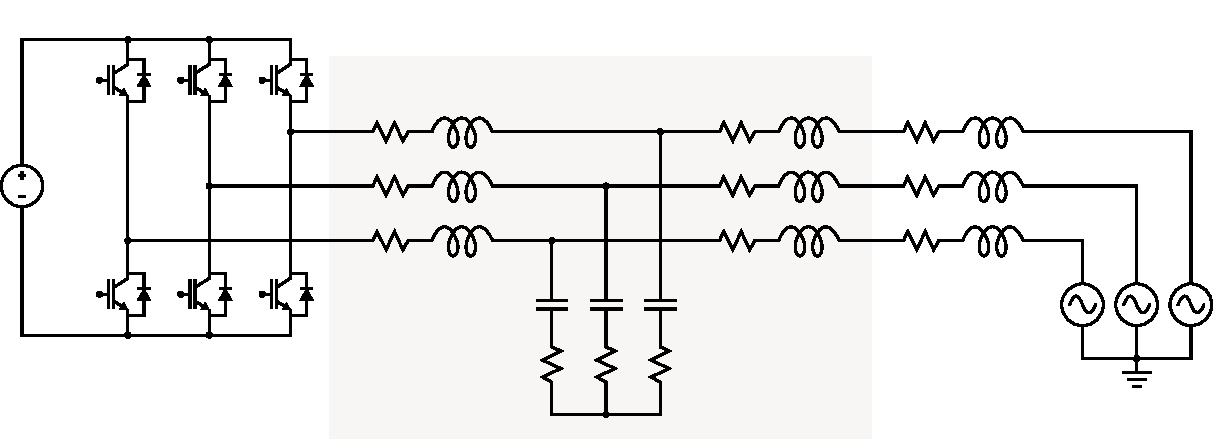
\includegraphics[width=0.9\textwidth]{img/topologia}}
      \def\svgwidth{0.9\textwidth}
      \input{./img/bancada.pdf_tex}}
    \renewcommand\figurename{Fig.}
    \caption{Diagrama que representa os elementos da bancada.}
    \label{fig:topologia_bancada}
  \end{figure}


\section{Resultados de Simulação}

	%figura mostrando o sistema
  %que tipo de conversor é, que marca, que modelo, dados nominais
  %que tipos de sensores foram usados? como foram feitas as medidas?
  %que tipo de controlador digital foi usado? modelo do dsp na dspace
  %quantos bits têm os conversores a/d?
  %como é acionado o conversor?
  %qual a frequência de amostragem? e a de comutação?
  %colocar numa tabela: tensão de linha, frequência, tensão do barramento cc, indutâncias e capacitância do filtro, frequência de amostragem e de comutação
  %comentar que os resultados obtidos foram para o equivalente monofásico
  %apresentar expressão do modelo de referência
  %apresentar expressões dos vetores w
  %apresentar os valores iniciais dos ganhos do controlador adaptativo (kp, gamma, rho, etc)
  %apresentar os valores de inicialização dos thetas
  %comentar sobre o sinal de normalização m^2

  O Simulink dispõe de muitos blocos cujos modelos matemáticos são geralmente aceitos como precisos o suficiente para representar elementos do mundo real. Por isso, os modelos de conversor, linha de transmissão, transformador e fonte são utilizados neste trabalho para representar o comportamento de elementos reais.

	A ação de controle é implementada na simulação via código escrito em linguagem própria do \textsc{Matlab}, chamada \textit{linguagem .m}. Existe um bloco no Simulink chamado \textit{Subsystem}, que recebe sinais de entrada e permite que esses sinais sejam manipulados via código para gerarem sinais de saída. Este bloco é utilizado para implementar a ação de controle projetada nos capítulos anteriores.

	Como a simulação é implementada em tempo discreto, os principais passos realizados são os seguintes:

	\begin{enumerate}
		\item \textit{Inicialização}: no início da simulação, são carregados os valores iniciais para as variáveis;
		\item \textit{Amostragem das variáveis}: as variáveis são amostradas para a realização dos cálculos preliminares da ação de controle;
    \item \textit{Conversão de coordenadas $abc$ para $\alpha \beta 0$}: é aplicada a transformação de desacoplamento nas variáveis;
		\item \textit{Cálculo da ação de controle}: a ação de controle é calculada e o estado atual das variáveis é armazenado como sendo o estado anterior para a próxima iteração da simulação;
    \item \textit{Acionamento do conversor}: a ação de controle é modulada por largura de pulso e as chaves do conversor são acionadas;
		\item \textit{Geração da saída}: são feitas as medidas da corrente e tensão do capacitor, e da corrente do lado da rede.
	\end{enumerate}

  O projeto do controlador é conforme o Capítulo~\ref{controle}. O modelo de referência projetado é da forma
  %
  \begin{equation}
    W_m(z) = \frac{(1-p_1)(1-p_2)}{(z-p_1)(z-p_2)}\text{,}
    \label{eq:wm_simulacao}
  \end{equation}
  %
  com $p_1 = p_2 = 0,2$.

	A Tabela~\ref{tab:parametros_projeto} resume os demais parâmetros utilizados no projeto. Os valores de inicialização dos parâmetros são baseadas nos valores ideais, ou seja, aqueles que fazem com que os valores dos ganhos adaptativos $\theta$ sejam $\theta^*$ (valores para a condição de casamento). Os valores de inicialização dos ganhos adaptativos, neste caso, são dados por \ref{eq:theta_ini}.
  %
  \begin{equation}
    \begin{split}
      \theta^T & = \left[ \begin{matrix} -0,03, & -0,36, & -0,57, & -0,01 & 0,16 & 0,02 \end{matrix} \right]\text{ e}\\
      \omega & = {\left[ \begin{matrix} 0 & 0 & 0 & 0 & 0 & 0 \end{matrix} \right]}^T\text{.}
    \end{split}
    \label{eq:theta_ini}
  \end{equation}

  \begin{table}[htb]
    \renewcommand{\arraystretch}{1.35}
    \setlength{\tabcolsep}{1.2mm}
    \caption{Valores dos parâmetros do sistema utilizados no projeto.}
    \label{tab:parametros_projeto}
    \centering
    \begin{tabular}{l l l l}
      \hline
      \multicolumn{1}{c}{Parâmetro} & \multicolumn{1}{c}{Valor} &
      \multicolumn{1}{c}{Parâmetro} & \multicolumn{1}{c}{Valor} \\
      \hline
      $L_1$      & $2$mH    & $L_2$         & $2$mH  \\
      $C$        & $40\mu$F & $f_s = 1/T_s$ & $12$kHz\\
      $\gamma_d$ & $0,0098$ & $\gamma$      & $0,99$ \\
      $\delta_0$ & $0,8$    &               & \\
      \hline
    \end{tabular}
  \end{table}

  %separar em três figuras, uma pra inversão de fase, outra pra degrau de amplitude e outra pra variação da indutância
  A Fig.~\ref{fig:i2_sim_ini} apresenta a corrente da rede em comparação com a referência. No instante $t_1 = \pi s$ ocorre inversão de fase na referência. A Fig.~\ref{fig:i2_simulacao_degrau} apresenta, no instante $t_2$, um degrau de amplitude aplicado à referência. Na Fig.~\ref{fig:i2_simulacao_L_rede} apresenta uma variação na indutância da rede no instante $t_3$.

	\begin{figure}[!htb]
    \centering
      \def\svgwidth{\textwidth}
      % This file was created by matlab2tikz v0.4.7 running on MATLAB 7.14.
% Copyright (c) 2008--2014, Nico Schlömer <nico.schloemer@gmail.com>
% All rights reserved.
% Minimal pgfplots version: 1.3
% 
% The latest updates can be retrieved from
%   http://www.mathworks.com/matlabcentral/fileexchange/22022-matlab2tikz
% where you can also make suggestions and rate matlab2tikz.
% 
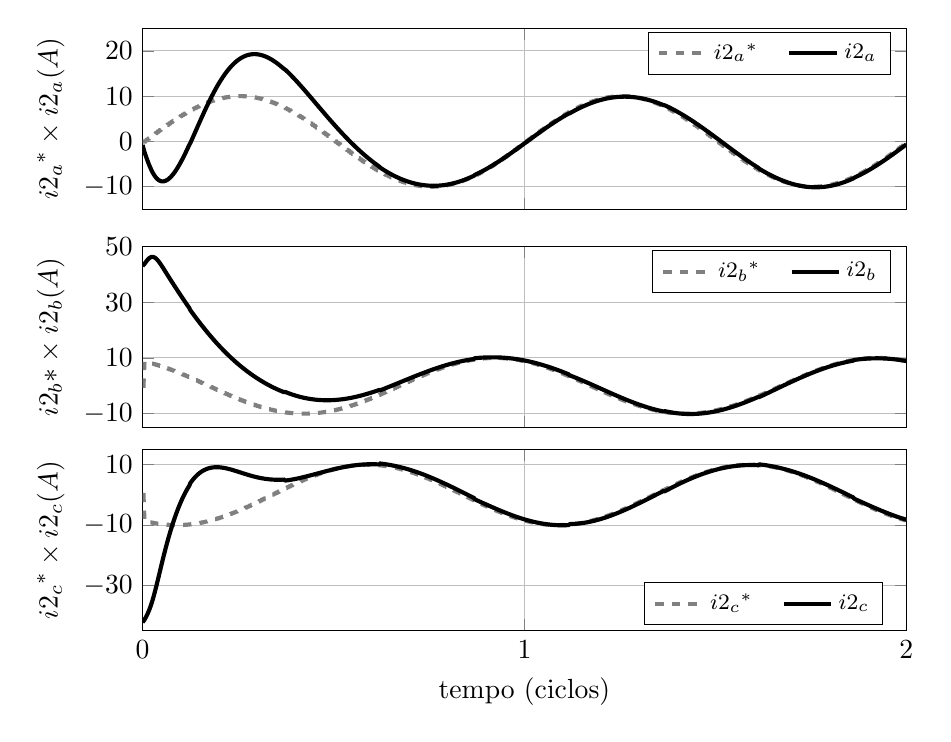
\begin{tikzpicture}

\begin{axis}[%
width=0.8\textwidth,
height=0.189701500343624\textwidth,
scale only axis,
xmin=0,
xmax=0.0333333333333333,
xtick={0,0.0166666666666667,0.0333333333333333},
xticklabels={\empty},
xmajorgrids,
ymin=-15,
ymax=50,
ytick={-10,  10,  30,  50},
ylabel={${\text{i2}_\text{b}}\text{* }\times\text{ i2}_\text{b}\text{ (A)}$},
ymajorgrids,
name=plot2,
legend style={draw=black,fill=white,legend cell align=left},
scaled x ticks = false,
legend columns=-1,
legend style={/tikz/every even column/.append style={column sep=0.3cm}},
legend style={font=\footnotesize}
]
\addplot [color=gray,dashed,line width=1.5pt]
  table[row sep=crcr]{0	0\\
4.16666666666667e-05	0\\
8.33333333333333e-05	8.66025403784439\\
0.000125	8.66025403784439\\
0.000166666666666667	8.49892692986864\\
0.000208333333333333	8.49892692986864\\
0.00025	8.329212407101\\
0.000291666666666667	8.329212407101\\
0.000333333333333333	8.15127795728554\\
0.000375	8.15127795728554\\
0.000416666666666667	7.96529918024197\\
0.000458333333333333	7.96529918024197\\
0.0005	7.77145961456971\\
0.000541666666666667	7.77145961456971\\
0.000583333333333333	7.56995055651757\\
0.000625	7.56995055651757\\
0.000666666666666667	7.36097087119735\\
0.000708333333333333	7.36097087119735\\
0.00075	7.14472679632804\\
0.000791666666666667	7.14472679632804\\
0.000833333333333333	6.92143173870407\\
0.000875	6.92143173870407\\
0.000916666666666667	6.69130606358858\\
0.000958333333333333	6.69130606358858\\
0.001	6.45457687723951\\
0.00104166666666667	6.45457687723951\\
0.00108333333333333	6.21147780278311\\
0.001125	6.21147780278311\\
0.00116666666666667	5.96224874965616\\
0.00120833333333333	5.96224874965616\\
0.00125	5.70713567684432\\
0.00129166666666667	5.70713567684432\\
0.00133333333333333	5.44639035015028\\
0.001375	5.44639035015028\\
0.00141666666666667	5.18027009373131\\
0.00145833333333333	5.18027009373131\\
0.0015	4.90903753615141\\
0.00154166666666667	4.90903753615141\\
0.00158333333333333	4.63296035119862\\
0.001625	4.63296035119862\\
0.00166666666666667	4.35231099372328\\
0.00170833333333333	4.35231099372328\\
0.00175	4.06736643075801\\
0.00179166666666667	4.06736643075801\\
0.00183333333333333	3.77840786818468\\
0.001875	3.77840786818468\\
0.00191666666666667	3.48572047321816\\
0.00195833333333333	3.48572047321816\\
0.002	3.18959309298071\\
0.00204166666666667	3.18959309298071\\
0.00208333333333333	2.89031796944472\\
0.002125	2.89031796944472\\
0.00216666666666667	2.58819045102521\\
0.00220833333333333	2.58819045102521\\
0.00225	2.28350870110656\\
0.00229166666666667	2.28350870110656\\
0.00233333333333333	1.97657340379127\\
0.002375	1.97657340379127\\
0.00241666666666667	1.66768746716103\\
0.00245833333333333	1.66768746716103\\
0.0025	1.35715572434305\\
0.00254166666666667	1.35715572434305\\
0.00258333333333333	1.04528463267654\\
0.002625	1.04528463267654\\
0.00266666666666667	0.732381971276321\\
0.00270833333333333	0.732381971276321\\
0.00275	0.418756537292\\
0.00279166666666667	0.418756537292\\
0.00283333333333333	0.104717841162462\\
0.002875	0.104717841162462\\
0.00291666666666667	-0.209424198833566\\
0.00295833333333333	-0.209424198833566\\
0.003	-0.523359562429436\\
0.00304166666666667	-0.523359562429436\\
0.00308333333333333	-0.836778433323153\\
0.003125	-0.836778433323153\\
0.00316666666666667	-1.14937150492867\\
0.00320833333333333	-1.14937150492867\\
0.00325	-1.46083028562412\\
0.00329166666666667	-1.46083028562412\\
0.00333333333333333	-1.77084740319583\\
0.003375	-1.77084740319583\\
0.00341666666666667	-2.07911690817759\\
0.00345833333333333	-2.07911690817759\\
0.0035	-2.38533457578581\\
0.00354166666666667	-2.38533457578581\\
0.00358333333333333	-2.68919820615266\\
0.003625	-2.68919820615266\\
0.00366666666666667	-2.99040792256087\\
0.00370833333333333	-2.99040792256087\\
0.00375	-3.28866646738584\\
0.00379166666666667	-3.28866646738584\\
0.00383333333333333	-3.58367949545301\\
0.003875	-3.58367949545301\\
0.00391666666666667	-3.87515586452103\\
0.00395833333333333	-3.87515586452103\\
0.004	-4.16280792260402\\
0.00404166666666667	-4.16280792260402\\
0.00408333333333333	-4.44635179184928\\
0.004125	-4.44635179184928\\
0.00416666666666667	-4.72550764869055\\
0.00420833333333333	-4.72550764869055\\
0.00425	-5.00000000000001\\
0.00429166666666667	-5.00000000000001\\
0.00433333333333333	-5.26955795496679\\
0.004375	-5.26955795496679\\
0.00441666666666667	-5.53391549243345\\
0.00445833333333333	-5.53391549243345\\
0.0045	-5.7928117234268\\
0.00454166666666667	-5.7928117234268\\
0.00458333333333333	-6.04599114862376\\
0.004625	-6.04599114862376\\
0.00466666666666667	-6.29320391049839\\
0.00470833333333333	-6.29320391049839\\
0.00475	-6.53420603990107\\
0.00479166666666667	-6.53420603990107\\
0.00483333333333333	-6.76875969682662\\
0.004875	-6.76875969682662\\
0.00491666666666667	-6.99663340513367\\
0.00495833333333333	-6.99663340513367\\
0.005	-7.21760228098364\\
0.00504166666666667	-7.21760228098364\\
0.00508333333333333	-7.43144825477396\\
0.005125	-7.43144825477396\\
0.00516666666666667	-7.63796028634644\\
0.00520833333333333	-7.63796028634644\\
0.00525	-7.83693457325842\\
0.00529166666666667	-7.83693457325842\\
0.00533333333333333	-8.02817475191117\\
0.005375	-8.02817475191117\\
0.00541666666666667	-8.21149209133706\\
0.00545833333333333	-8.21149209133706\\
0.0055	-8.38670567945426\\
0.00554166666666667	-8.38670567945426\\
0.00558333333333333	-8.55364260160509\\
0.005625	-8.55364260160509\\
0.00566666666666667	-8.71213811120192\\
0.00570833333333333	-8.71213811120192\\
0.00575	-8.86203579231217\\
0.00579166666666667	-8.86203579231217\\
0.00583333333333333	-9.00318771402196\\
0.005875	-9.00318771402196\\
0.00591666666666667	-9.13545457642604\\
0.00595833333333333	-9.13545457642604\\
0.006	-9.25870584809998\\
0.00604166666666667	-9.25870584809998\\
0.00608333333333333	-9.37281989491894\\
0.006125	-9.37281989491894\\
0.00616666666666667	-9.47768410009589\\
0.00620833333333333	-9.47768410009589\\
0.00625	-9.5731949753207\\
0.00629166666666667	-9.5731949753207\\
0.00633333333333333	-9.65925826289071\\
0.006375	-9.65925826289071\\
0.00641666666666667	-9.73578902873164\\
0.00645833333333333	-9.73578902873164\\
0.0065	-9.80271174621725\\
0.00654166666666667	-9.80271174621725\\
0.00658333333333333	-9.85996037070508\\
0.006625	-9.85996037070508\\
0.00666666666666667	-9.90747840471447\\
0.00670833333333333	-9.90747840471447\\
0.00675	-9.94521895368277\\
0.00679166666666667	-9.94521895368277\\
0.00683333333333333	-9.97314477224462\\
0.006875	-9.97314477224462\\
0.00691666666666667	-9.99122830098862\\
0.00695833333333333	-9.99122830098862\\
0.007	-9.99945169365516\\
0.00704166666666667	-9.99945169365516\\
0.00708333333333333	-9.99780683474849\\
0.007125	-9.99780683474849\\
0.00716666666666667	-9.98629534754578\\
0.00720833333333333	-9.98629534754578\\
0.00725	-9.96492859249508\\
0.00729166666666667	-9.96492859249508\\
0.00733333333333333	-9.93372765600401\\
0.007375	-9.93372765600401\\
0.00741666666666667	-9.89272332962993\\
0.00745833333333333	-9.89272332962993\\
0.0075	-9.84195607969246\\
0.00754166666666667	-9.84195607969246\\
0.00758333333333333	-9.7814760073381\\
0.007625	-9.7814760073381\\
0.00766666666666667	-9.7113427990964\\
0.00770833333333333	-9.7113427990964\\
0.00775	-9.63162566797663\\
0.00779166666666667	-9.63162566797663\\
0.00783333333333333	-9.54240328516281\\
0.007875	-9.54240328516281\\
0.00791666666666667	-9.44376370237485\\
0.00795833333333333	-9.44376370237485\\
0.008	-9.33580426497206\\
0.00804166666666667	-9.33580426497206\\
0.00808333333333333	-9.21863151588505\\
0.008125	-9.21863151588505\\
0.00816666666666667	-9.09236109047073\\
0.00820833333333333	-9.09236109047073\\
0.00825	-8.95711760239417\\
0.00829166666666667	-8.95711760239417\\
0.00833333333333333	-8.81303452064997\\
0.008375	-8.81303452064997\\
0.00841666666666667	-8.66025403784443\\
0.00845833333333333	-8.66025403784443\\
0.0085	-8.49892692986868\\
0.00854166666666667	-8.49892692986868\\
0.00858333333333333	-8.32921240710104\\
0.008625	-8.32921240710104\\
0.00866666666666667	-8.15127795728559\\
0.00870833333333333	-8.15127795728559\\
0.00875	-7.965299180242\\
0.00879166666666667	-7.965299180242\\
0.00883333333333333	-7.77145961456975\\
0.008875	-7.77145961456975\\
0.00891666666666667	-7.56995055651761\\
0.00895833333333333	-7.56995055651761\\
0.009	-7.36097087119738\\
0.00904166666666667	-7.36097087119738\\
0.00908333333333333	-7.14472679632807\\
0.009125	-7.14472679632807\\
0.00916666666666667	-6.92143173870411\\
0.00920833333333333	-6.92143173870411\\
0.00925	-6.69130606358862\\
0.00929166666666667	-6.69130606358862\\
0.00933333333333333	-6.45457687723954\\
0.009375	-6.45457687723954\\
0.00941666666666667	-6.21147780278314\\
0.00945833333333333	-6.21147780278314\\
0.0095	-5.96224874965619\\
0.00954166666666667	-5.96224874965619\\
0.00958333333333333	-5.70713567684435\\
0.009625	-5.70713567684435\\
0.00966666666666667	-5.4463903501503\\
0.00970833333333333	-5.4463903501503\\
0.00975	-5.18027009373134\\
0.00979166666666667	-5.18027009373134\\
0.00983333333333333	-4.90903753615144\\
0.009875	-4.90903753615144\\
0.00991666666666667	-4.63296035119865\\
0.00995833333333333	-4.63296035119865\\
0.01	-4.35231099372331\\
0.0100416666666667	-4.35231099372331\\
0.0100833333333333	-4.06736643075803\\
0.010125	-4.06736643075803\\
0.0101666666666667	-3.7784078681847\\
0.0102083333333333	-3.7784078681847\\
0.01025	-3.48572047321818\\
0.0102916666666667	-3.48572047321818\\
0.0103333333333333	-3.18959309298072\\
0.010375	-3.18959309298072\\
0.0104166666666667	-2.89031796944474\\
0.0104583333333333	-2.89031796944474\\
0.0105	-2.58819045102523\\
0.0105416666666667	-2.58819045102523\\
0.0105833333333333	-2.28350870110658\\
0.010625	-2.28350870110658\\
0.0106666666666667	-1.97657340379128\\
0.0107083333333333	-1.97657340379128\\
0.01075	-1.66768746716104\\
0.0107916666666667	-1.66768746716104\\
0.0108333333333333	-1.35715572434306\\
0.010875	-1.35715572434306\\
0.0109166666666667	-1.04528463267655\\
0.0109583333333333	-1.04528463267655\\
0.011	-0.732381971276329\\
0.0110416666666667	-0.732381971276329\\
0.0110833333333333	-0.418756537292006\\
0.011125	-0.418756537292006\\
0.0111666666666667	-0.104717841162466\\
0.0112083333333333	-0.104717841162466\\
0.01125	0.209424198833563\\
0.0112916666666667	0.209424198833563\\
0.0113333333333333	0.523359562429434\\
0.011375	0.523359562429434\\
0.0114166666666667	0.836778433323152\\
0.0114583333333333	0.836778433323152\\
0.0115	1.14937150492867\\
0.0115416666666667	1.14937150492867\\
0.0115833333333333	1.46083028562412\\
0.011625	1.46083028562412\\
0.0116666666666667	1.77084740319584\\
0.0117083333333333	1.77084740319584\\
0.01175	2.0791169081776\\
0.0117916666666667	2.0791169081776\\
0.0118333333333333	2.38533457578582\\
0.011875	2.38533457578582\\
0.0119166666666667	2.68919820615266\\
0.0119583333333333	2.68919820615266\\
0.012	2.99040792256088\\
0.0120416666666667	2.99040792256088\\
0.0120833333333333	3.28866646738584\\
0.012125	3.28866646738584\\
0.0121666666666667	3.58367949545302\\
0.0122083333333333	3.58367949545302\\
0.01225	3.87515586452105\\
0.0122916666666667	3.87515586452105\\
0.0123333333333333	4.16280792260403\\
0.012375	4.16280792260403\\
0.0124166666666667	4.4463517918493\\
0.0124583333333333	4.4463517918493\\
0.0125	4.72550764869056\\
0.0125416666666667	4.72550764869056\\
0.0125833333333333	5.00000000000002\\
0.012625	5.00000000000002\\
0.0126666666666667	5.2695579549668\\
0.0127083333333333	5.2695579549668\\
0.01275	5.53391549243347\\
0.0127916666666667	5.53391549243347\\
0.0128333333333333	5.79281172342682\\
0.012875	5.79281172342682\\
0.0129166666666667	6.04599114862378\\
0.0129583333333333	6.04599114862378\\
0.013	6.29320391049841\\
0.0130416666666667	6.29320391049841\\
0.0130833333333333	6.53420603990109\\
0.013125	6.53420603990109\\
0.0131666666666667	6.76875969682665\\
0.0132083333333333	6.76875969682665\\
0.01325	6.99663340513369\\
0.0132916666666667	6.99663340513369\\
0.0133333333333333	7.21760228098367\\
0.013375	7.21760228098367\\
0.0134166666666667	7.43144825477399\\
0.0134583333333333	7.43144825477399\\
0.0135	7.63796028634647\\
0.0135416666666667	7.63796028634647\\
0.0135833333333333	7.83693457325845\\
0.013625	7.83693457325845\\
0.0136666666666667	8.02817475191119\\
0.0137083333333333	8.02817475191119\\
0.01375	8.21149209133709\\
0.0137916666666667	8.21149209133709\\
0.0138333333333333	8.38670567945429\\
0.013875	8.38670567945429\\
0.0139166666666667	8.55364260160512\\
0.0139583333333333	8.55364260160512\\
0.014	8.71213811120195\\
0.0140416666666667	8.71213811120195\\
0.0140833333333333	8.86203579231221\\
0.014125	8.86203579231221\\
0.0141666666666667	9.003187714022\\
0.0142083333333333	9.003187714022\\
0.01425	9.13545457642607\\
0.0142916666666667	9.13545457642607\\
0.0143333333333333	9.25870584810001\\
0.014375	9.25870584810001\\
0.0144166666666667	9.37281989491898\\
0.0144583333333333	9.37281989491898\\
0.0145	9.47768410009592\\
0.0145416666666667	9.47768410009592\\
0.0145833333333333	9.57319497532074\\
0.014625	9.57319497532074\\
0.0146666666666667	9.65925826289075\\
0.0147083333333333	9.65925826289075\\
0.01475	9.73578902873167\\
0.0147916666666667	9.73578902873167\\
0.0148333333333333	9.80271174621729\\
0.014875	9.80271174621729\\
0.0149166666666667	9.85996037070512\\
0.0149583333333333	9.85996037070512\\
0.015	9.90747840471451\\
0.0150416666666667	9.90747840471451\\
0.0150833333333333	9.94521895368281\\
0.015125	9.94521895368281\\
0.0151666666666667	9.97314477224466\\
0.0152083333333333	9.97314477224466\\
0.01525	9.99122830098866\\
0.0152916666666667	9.99122830098866\\
0.0153333333333333	9.9994516936552\\
0.015375	9.9994516936552\\
0.0154166666666667	9.99780683474853\\
0.0154583333333333	9.99780683474853\\
0.0155	9.98629534754582\\
0.0155416666666667	9.98629534754582\\
0.0155833333333333	9.96492859249513\\
0.015625	9.96492859249513\\
0.0156666666666667	9.93372765600405\\
0.0157083333333333	9.93372765600405\\
0.01575	9.89272332962997\\
0.0157916666666667	9.89272332962997\\
0.0158333333333333	9.8419560796925\\
0.015875	9.8419560796925\\
0.0159166666666667	9.78147600733814\\
0.0159583333333333	9.78147600733814\\
0.016	9.71134279909644\\
0.0160416666666667	9.71134279909644\\
0.0160833333333333	9.63162566797667\\
0.016125	9.63162566797667\\
0.0161666666666667	9.54240328516285\\
0.0162083333333333	9.54240328516285\\
0.01625	9.44376370237489\\
0.0162916666666667	9.44376370237489\\
0.0163333333333333	9.3358042649721\\
0.016375	9.3358042649721\\
0.0164166666666667	9.21863151588509\\
0.0164583333333333	9.21863151588509\\
0.0165	9.09236109047077\\
0.0165416666666667	9.09236109047077\\
0.0165833333333333	8.95711760239421\\
0.016625	8.95711760239421\\
0.0166666666666667	8.81303452065\\
0.0167083333333333	8.81303452065\\
0.01675	8.66025403784447\\
0.0167916666666667	8.66025403784447\\
0.0168333333333333	8.49892692986872\\
0.016875	8.49892692986872\\
0.0169166666666667	8.32921240710107\\
0.0169583333333333	8.32921240710107\\
0.017	8.15127795728562\\
0.0170416666666667	8.15127795728562\\
0.0170833333333333	7.96529918024204\\
0.017125	7.96529918024204\\
0.0171666666666667	7.77145961456979\\
0.0172083333333333	7.77145961456979\\
0.01725	7.56995055651764\\
0.0172916666666667	7.56995055651764\\
0.0173333333333333	7.36097087119742\\
0.017375	7.36097087119742\\
0.0174166666666667	7.1447267963281\\
0.0174583333333333	7.1447267963281\\
0.0175	6.92143173870414\\
0.0175416666666667	6.92143173870414\\
0.0175833333333333	6.69130606358865\\
0.017625	6.69130606358865\\
0.0176666666666667	6.45457687723957\\
0.0177083333333333	6.45457687723957\\
0.01775	6.21147780278317\\
0.0177916666666667	6.21147780278317\\
0.0178333333333333	5.96224874965622\\
0.017875	5.96224874965622\\
0.0179166666666667	5.70713567684438\\
0.0179583333333333	5.70713567684438\\
0.018	5.44639035015033\\
0.0180416666666667	5.44639035015033\\
0.0180833333333333	5.18027009373136\\
0.018125	5.18027009373136\\
0.0181666666666667	4.90903753615147\\
0.0182083333333333	4.90903753615147\\
0.01825	4.63296035119867\\
0.0182916666666667	4.63296035119867\\
0.0183333333333333	4.35231099372333\\
0.018375	4.35231099372333\\
0.0184166666666667	4.06736643075805\\
0.0184583333333333	4.06736643075805\\
0.0185	3.77840786818472\\
0.0185416666666667	3.77840786818472\\
0.0185833333333333	3.4857204732182\\
0.018625	3.4857204732182\\
0.0186666666666667	3.18959309298074\\
0.0187083333333333	3.18959309298074\\
0.01875	2.89031796944476\\
0.0187916666666667	2.89031796944476\\
0.0188333333333333	2.58819045102524\\
0.018875	2.58819045102524\\
0.0189166666666667	2.28350870110659\\
0.0189583333333333	2.28350870110659\\
0.019	1.97657340379129\\
0.0190416666666667	1.97657340379129\\
0.0190833333333333	1.66768746716105\\
0.019125	1.66768746716105\\
0.0191666666666667	1.35715572434307\\
0.0192083333333333	1.35715572434307\\
0.01925	1.04528463267656\\
0.0192916666666667	1.04528463267656\\
0.0193333333333333	0.732381971276336\\
0.019375	0.732381971276336\\
0.0194166666666667	0.418756537292012\\
0.0194583333333333	0.418756537292012\\
0.0195	0.104717841162471\\
0.0195416666666667	0.104717841162471\\
0.0195833333333333	-0.20942419883356\\
0.019625	-0.20942419883356\\
0.0196666666666667	-0.523359562429432\\
0.0197083333333333	-0.523359562429432\\
0.01975	-0.836778433323152\\
0.0197916666666667	-0.836778433323152\\
0.0198333333333333	-1.14937150492867\\
0.019875	-1.14937150492867\\
0.0199166666666667	-1.46083028562412\\
0.0199583333333333	-1.46083028562412\\
0.02	-1.77084740319584\\
0.0200416666666667	-1.77084740319584\\
0.0200833333333333	-2.0791169081776\\
0.020125	-2.0791169081776\\
0.0201666666666667	-2.38533457578582\\
0.0202083333333333	-2.38533457578582\\
0.02025	-2.68919820615267\\
0.0202916666666667	-2.68919820615267\\
0.0203333333333333	-2.99040792256089\\
0.020375	-2.99040792256089\\
0.0204166666666667	-3.28866646738586\\
0.0204583333333333	-3.28866646738586\\
0.0205	-3.58367949545303\\
0.0205416666666667	-3.58367949545303\\
0.0205833333333333	-3.87515586452106\\
0.020625	-3.87515586452106\\
0.0206666666666667	-4.16280792260405\\
0.0207083333333333	-4.16280792260405\\
0.02075	-4.44635179184931\\
0.0207916666666667	-4.44635179184931\\
0.0208333333333333	-4.72550764869058\\
0.020875	-4.72550764869058\\
0.0209166666666667	-5.00000000000005\\
0.0209583333333333	-5.00000000000005\\
0.021	-5.26955795496682\\
0.0210416666666667	-5.26955795496682\\
0.0210833333333333	-5.53391549243349\\
0.021125	-5.53391549243349\\
0.0211666666666667	-5.79281172342684\\
0.0212083333333333	-5.79281172342684\\
0.02125	-6.0459911486238\\
0.0212916666666667	-6.0459911486238\\
0.0213333333333333	-6.29320391049844\\
0.021375	-6.29320391049844\\
0.0214166666666667	-6.53420603990112\\
0.0214583333333333	-6.53420603990112\\
0.0215	-6.76875969682667\\
0.0215416666666667	-6.76875969682667\\
0.0215833333333333	-6.99663340513372\\
0.021625	-6.99663340513372\\
0.0216666666666667	-7.2176022809837\\
0.0217083333333333	-7.2176022809837\\
0.02175	-7.43144825477402\\
0.0217916666666667	-7.43144825477402\\
0.0218333333333333	-7.6379602863465\\
0.021875	-7.6379602863465\\
0.0219166666666667	-7.83693457325848\\
0.0219583333333333	-7.83693457325848\\
0.022	-8.02817475191123\\
0.0220416666666667	-8.02817475191123\\
0.0220833333333333	-8.21149209133713\\
0.022125	-8.21149209133713\\
0.0221666666666667	-8.38670567945433\\
0.0222083333333333	-8.38670567945433\\
0.02225	-8.55364260160516\\
0.0222916666666667	-8.55364260160516\\
0.0223333333333333	-8.71213811120199\\
0.022375	-8.71213811120199\\
0.0224166666666667	-8.86203579231225\\
0.0224583333333333	-8.86203579231225\\
0.0225	-9.00318771402204\\
0.0225416666666667	-9.00318771402204\\
0.0225833333333333	-9.13545457642611\\
0.022625	-9.13545457642611\\
0.0226666666666667	-9.25870584810006\\
0.0227083333333333	-9.25870584810006\\
0.02275	-9.37281989491902\\
0.0227916666666667	-9.37281989491902\\
0.0228333333333333	-9.47768410009597\\
0.022875	-9.47768410009597\\
0.0229166666666667	-9.57319497532079\\
0.0229583333333333	-9.57319497532079\\
0.023	-9.6592582628908\\
0.0230416666666667	-9.6592582628908\\
0.0230833333333333	-9.73578902873172\\
0.023125	-9.73578902873172\\
0.0231666666666667	-9.80271174621734\\
0.0232083333333333	-9.80271174621734\\
0.02325	-9.85996037070517\\
0.0232916666666667	-9.85996037070517\\
0.0233333333333333	-9.90747840471456\\
0.023375	-9.90747840471456\\
0.0234166666666667	-9.94521895368285\\
0.0234583333333333	-9.94521895368285\\
0.0235	-9.97314477224471\\
0.0235416666666667	-9.97314477224471\\
0.0235833333333333	-9.99122830098871\\
0.023625	-9.99122830098871\\
0.0236666666666667	-9.99945169365525\\
0.0237083333333333	-9.99945169365525\\
0.02375	-9.99780683474858\\
0.0237916666666667	-9.99780683474858\\
0.0238333333333333	-9.98629534754587\\
0.023875	-9.98629534754587\\
0.0239166666666667	-9.96492859249517\\
0.0239583333333333	-9.96492859249517\\
0.024	-9.93372765600409\\
0.0240416666666667	-9.93372765600409\\
0.0240833333333333	-9.89272332963001\\
0.024125	-9.89272332963001\\
0.0241666666666667	-9.84195607969255\\
0.0242083333333333	-9.84195607969255\\
0.02425	-9.78147600733818\\
0.0242916666666667	-9.78147600733818\\
0.0243333333333333	-9.71134279909649\\
0.024375	-9.71134279909649\\
0.0244166666666667	-9.63162566797671\\
0.0244583333333333	-9.63162566797671\\
0.0245	-9.5424032851629\\
0.0245416666666667	-9.5424032851629\\
0.0245833333333333	-9.44376370237494\\
0.024625	-9.44376370237494\\
0.0246666666666667	-9.33580426497215\\
0.0247083333333333	-9.33580426497215\\
0.02475	-9.21863151588513\\
0.0247916666666667	-9.21863151588513\\
0.0248333333333333	-9.09236109047081\\
0.024875	-9.09236109047081\\
0.0249166666666667	-8.95711760239425\\
0.0249583333333333	-8.95711760239425\\
0.025	-8.81303452065005\\
0.0250416666666667	-8.81303452065005\\
0.0250833333333333	-8.66025403784451\\
0.025125	-8.66025403784451\\
0.0251666666666667	-8.49892692986876\\
0.0252083333333333	-8.49892692986876\\
0.02525	-8.32921240710111\\
0.0252916666666667	-8.32921240710111\\
0.0253333333333333	-8.15127795728566\\
0.025375	-8.15127795728566\\
0.0254166666666667	-7.96529918024207\\
0.0254583333333333	-7.96529918024207\\
0.0255	-7.77145961456982\\
0.0255416666666667	-7.77145961456982\\
0.0255833333333333	-7.56995055651767\\
0.025625	-7.56995055651767\\
0.0256666666666667	-7.36097087119745\\
0.0257083333333333	-7.36097087119745\\
0.02575	-7.14472679632814\\
0.0257916666666667	-7.14472679632814\\
0.0258333333333333	-6.92143173870417\\
0.025875	-6.92143173870417\\
0.0259166666666667	-6.69130606358868\\
0.0259583333333333	-6.69130606358868\\
0.026	-6.4545768772396\\
0.0260416666666667	-6.4545768772396\\
0.0260833333333333	-6.2114778027832\\
0.026125	-6.2114778027832\\
0.0261666666666667	-5.96224874965625\\
0.0262083333333333	-5.96224874965625\\
0.02625	-5.70713567684441\\
0.0262916666666667	-5.70713567684441\\
0.0263333333333333	-5.44639035015036\\
0.026375	-5.44639035015036\\
0.0264166666666667	-5.18027009373139\\
0.0264583333333333	-5.18027009373139\\
0.0265	-4.90903753615149\\
0.0265416666666667	-4.90903753615149\\
0.0265833333333333	-4.6329603511987\\
0.026625	-4.6329603511987\\
0.0266666666666667	-4.35231099372335\\
0.0267083333333333	-4.35231099372335\\
0.02675	-4.06736643075807\\
0.0267916666666667	-4.06736643075807\\
0.0268333333333333	-3.77840786818474\\
0.026875	-3.77840786818474\\
0.0269166666666667	-3.48572047321821\\
0.0269583333333333	-3.48572047321821\\
0.027	-3.18959309298076\\
0.0270416666666667	-3.18959309298076\\
0.0270833333333333	-2.89031796944477\\
0.027125	-2.89031796944477\\
0.0271666666666667	-2.58819045102526\\
0.0272083333333333	-2.58819045102526\\
0.02725	-2.28350870110661\\
0.0272916666666667	-2.28350870110661\\
0.0273333333333333	-1.9765734037913\\
0.027375	-1.9765734037913\\
0.0274166666666667	-1.66768746716106\\
0.0274583333333333	-1.66768746716106\\
0.0275	-1.35715572434308\\
0.0275416666666667	-1.35715572434308\\
0.0275833333333333	-1.04528463267656\\
0.027625	-1.04528463267656\\
0.0276666666666667	-0.732381971276341\\
0.0277083333333333	-0.732381971276341\\
0.02775	-0.418756537292015\\
0.0277916666666667	-0.418756537292015\\
0.0278333333333333	-0.104717841162473\\
0.027875	-0.104717841162473\\
0.0279166666666667	0.209424198833559\\
0.0279583333333333	0.209424198833559\\
0.028	0.523359562429433\\
0.0280416666666667	0.523359562429433\\
0.0280833333333333	0.836778433323154\\
0.028125	0.836778433323154\\
0.0281666666666667	1.14937150492867\\
0.0282083333333333	1.14937150492867\\
0.02825	1.46083028562412\\
0.0282916666666667	1.46083028562412\\
0.0283333333333333	1.77084740319585\\
0.028375	1.77084740319585\\
0.0284166666666667	2.07911690817761\\
0.0284583333333333	2.07911690817761\\
0.0285	2.38533457578583\\
0.0285416666666667	2.38533457578583\\
0.0285833333333333	2.68919820615268\\
0.028625	2.68919820615268\\
0.0286666666666667	2.9904079225609\\
0.0287083333333333	2.9904079225609\\
0.02875	3.28866646738587\\
0.0287916666666667	3.28866646738587\\
0.0288333333333333	3.58367949545304\\
0.028875	3.58367949545304\\
0.0289166666666667	3.87515586452107\\
0.0289583333333333	3.87515586452107\\
0.029	4.16280792260406\\
0.0290416666666667	4.16280792260406\\
0.0290833333333333	4.44635179184933\\
0.029125	4.44635179184933\\
0.0291666666666667	4.7255076486906\\
0.0292083333333333	4.7255076486906\\
0.02925	5.00000000000006\\
0.0292916666666667	5.00000000000006\\
0.0293333333333333	5.26955795496684\\
0.029375	5.26955795496684\\
0.0294166666666667	5.53391549243351\\
0.0294583333333333	5.53391549243351\\
0.0295	5.79281172342686\\
0.0295416666666667	5.79281172342686\\
0.0295833333333333	6.04599114862383\\
0.029625	6.04599114862383\\
0.0296666666666667	6.29320391049846\\
0.0297083333333333	6.29320391049846\\
0.02975	6.53420603990114\\
0.0297916666666667	6.53420603990114\\
0.0298333333333333	6.7687596968267\\
0.029875	6.7687596968267\\
0.0299166666666667	6.99663340513375\\
0.0299583333333333	6.99663340513375\\
0.03	7.21760228098372\\
0.0300416666666667	7.21760228098372\\
0.0300833333333333	7.43144825477405\\
0.030125	7.43144825477405\\
0.0301666666666667	7.63796028634653\\
0.0302083333333333	7.63796028634653\\
0.03025	7.83693457325851\\
0.0302916666666667	7.83693457325851\\
0.0303333333333333	8.02817475191126\\
0.030375	8.02817475191126\\
0.0304166666666667	8.21149209133716\\
0.0304583333333333	8.21149209133716\\
0.0305	8.38670567945436\\
0.0305416666666667	8.38670567945436\\
0.0305833333333333	8.55364260160519\\
0.030625	8.55364260160519\\
0.0306666666666667	8.71213811120203\\
0.0307083333333333	8.71213811120203\\
0.03075	8.86203579231228\\
0.0307916666666667	8.86203579231228\\
0.0308333333333333	9.00318771402207\\
0.030875	9.00318771402207\\
0.0309166666666667	9.13545457642615\\
0.0309583333333333	9.13545457642615\\
0.031	9.25870584810009\\
0.0310416666666667	9.25870584810009\\
0.0310833333333333	9.37281989491906\\
0.031125	9.37281989491906\\
0.0311666666666667	9.477684100096\\
0.0312083333333333	9.477684100096\\
0.03125	9.57319497532082\\
0.0312916666666667	9.57319497532082\\
0.0313333333333333	9.65925826289084\\
0.031375	9.65925826289084\\
0.0314166666666667	9.73578902873176\\
0.0314583333333333	9.73578902873176\\
0.0315	9.80271174621738\\
0.0315416666666667	9.80271174621738\\
0.0315833333333333	9.85996037070521\\
0.031625	9.85996037070521\\
0.0316666666666667	9.9074784047146\\
0.0317083333333333	9.9074784047146\\
0.03175	9.94521895368289\\
0.0317916666666667	9.94521895368289\\
0.0318333333333333	9.97314477224474\\
0.031875	9.97314477224474\\
0.0319166666666667	9.99122830098875\\
0.0319583333333333	9.99122830098875\\
0.032	9.99945169365528\\
0.0320416666666667	9.99945169365528\\
0.0320833333333333	9.99780683474862\\
0.032125	9.99780683474862\\
0.0321666666666667	9.98629534754591\\
0.0322083333333333	9.98629534754591\\
0.03225	9.96492859249521\\
0.0322916666666667	9.96492859249521\\
0.0323333333333333	9.93372765600413\\
0.032375	9.93372765600413\\
0.0324166666666667	9.89272332963005\\
0.0324583333333333	9.89272332963005\\
0.0325	9.84195607969259\\
0.0325416666666667	9.84195607969259\\
0.0325833333333333	9.78147600733822\\
0.032625	9.78147600733822\\
0.0326666666666667	9.71134279909653\\
0.0327083333333333	9.71134279909653\\
0.03275	9.63162566797675\\
0.0327916666666667	9.63162566797675\\
0.0328333333333333	9.54240328516294\\
0.032875	9.54240328516294\\
0.0329166666666667	9.44376370237498\\
0.0329583333333333	9.44376370237498\\
0.033	9.33580426497218\\
0.0330416666666667	9.33580426497218\\
0.0330833333333333	9.21863151588517\\
0.033125	9.21863151588517\\
0.0331666666666667	9.09236109047085\\
0.0332083333333333	9.09236109047085\\
0.03325	8.95711760239429\\
0.0332916666666667	8.95711760239429\\
0.0333333333333333	8.81303452065008\\
};
\addlegendentry{${\text{i2}_\text{b}}^\text{*}$};

\addplot [color=black,solid,line width=1.5pt]
  table[row sep=crcr]{0	42.97660421501\\
4.16666666666667e-05	43.3593393870968\\
8.33333333333333e-05	43.7191880113411\\
0.000125	44.2050613899279\\
0.000166666666666667	44.6603456269382\\
0.000208333333333333	45.1018552556462\\
0.00025	45.48220841885\\
0.000291666666666667	45.8113981893254\\
0.000333333333333333	46.0508290702559\\
0.000375	46.2155916866694\\
0.000416666666666667	46.2794096603762\\
0.000458333333333333	46.2638806240286\\
0.0005	46.151102640534\\
0.000541666666666667	45.9672904475899\\
0.000583333333333333	45.7004204890381\\
0.000625	45.3784996924376\\
0.000666666666666667	44.9925737085849\\
0.000708333333333333	44.569792657511\\
0.00075	44.1021229439723\\
0.000791666666666667	43.6140575421866\\
0.000833333333333333	43.0972531042803\\
0.000875	42.5727018637345\\
0.000916666666666667	42.0313491398431\\
0.000958333333333333	41.490604512486\\
0.001	40.9408606766391\\
0.00104166666666667	40.3963231914932\\
0.00108333333333333	39.847267627143\\
0.001125	39.3052673895989\\
0.00116666666666667	38.7609604462391\\
0.00120833333333333	38.223851996809\\
0.00125	37.6853493581397\\
0.00129166666666667	37.1533454635223\\
0.00133333333333333	36.6202871491275\\
0.001375	36.0927730404365\\
0.00141666666666667	35.5644250721109\\
0.00145833333333333	35.0407402121898\\
0.0015	34.5165453424891\\
0.00154166666666667	33.9963369942111\\
0.00158333333333333	33.4761083185055\\
0.001625	32.9594021528808\\
0.00166666666666667	32.4433041643775\\
0.00170833333333333	31.930426082963\\
0.00175	31.4188614749057\\
0.00179166666666667	30.9103095974188\\
0.00183333333333333	30.4037906684295\\
0.001875	29.9001167441415\\
0.00191666666666667	29.3991629296628\\
0.00195833333333333	28.9008893757573\\
0.002	28.4059645531346\\
0.00204166666666667	27.9135410549802\\
0.00208333333333333	27.1721535020907\\
0.002125	26.6874505908316\\
0.00216666666666667	26.2190588726424\\
0.00220833333333333	25.7486586212972\\
0.00225	25.2853868986719\\
0.00229166666666667	24.8230429289484\\
0.00233333333333333	24.3666319292948\\
0.002375	23.9112946756842\\
0.00241666666666667	23.4618362846351\\
0.00245833333333333	23.013304313649\\
0.0025	22.5707908845547\\
0.00254166666666667	22.1290599227619\\
0.00258333333333333	21.6935327273799\\
0.002625	21.2586693811889\\
0.00266666666666667	20.8302050849802\\
0.00270833333333333	20.4023045251397\\
0.00275	19.9809941762427\\
0.00279166666666667	19.5601600656416\\
0.00283333333333333	19.1460961574073\\
0.002875	18.7324306257852\\
0.00291666666666667	18.3257006249585\\
0.00295833333333333	17.9192996196269\\
0.003	17.5199832279738\\
0.00304166666666667	17.1209346176351\\
0.00308333333333333	16.7291028297554\\
0.003125	16.3374695704814\\
0.00316666666666667	15.9531836896215\\
0.00320833333333333	15.5690705398771\\
0.00325	15.1923861917557\\
0.00329166666666667	14.8158333649373\\
0.00333333333333333	14.4467915071034\\
0.003375	14.0778495809671\\
0.00341666666666667	13.716482665951\\
0.00345833333333333	13.3551909497519\\
0.0035	13.0015211738397\\
0.00354166666666667	12.6479078035316\\
0.00358333333333333	12.3019466802048\\
0.003625	11.9560285381684\\
0.00366666666666667	11.6177769520913\\
0.00370833333333333	11.2795599226045\\
0.00375	10.9490085867896\\
0.00379166666666667	10.6184881556411\\
0.00383333333333333	10.2956183498002\\
0.003875	9.97278041548817\\
0.00391666666666667	9.65756485851209\\
0.00395833333333333	9.34238662156467\\
0.004	9.0347903657762\\
0.00404166666666667	8.72724120879229\\
0.00408333333333333	8.4272224949194\\
0.004125	8.12726481447167\\
0.00416666666666667	7.83521349471893\\
0.00420833333333333	7.54285122194898\\
0.00425	7.2578778410272\\
0.00429166666666667	6.97299745656387\\
0.00433333333333333	6.69542553982568\\
0.004375	6.41795837374215\\
0.00441666666666667	6.14769031764613\\
0.00445833333333333	5.87752475840982\\
0.0045	5.61442748637277\\
0.00454166666666667	5.35142369057221\\
0.00458333333333333	5.09534751453348\\
0.004625	4.83935958306598\\
0.00466666666666667	4.59015883100606\\
0.00470833333333333	4.34105278963748\\
0.00475	4.09860077797683\\
0.00479166666666667	3.856265899529\\
0.00483333333333333	3.62046245805827\\
0.004875	3.38481516617511\\
0.00491666666666667	3.1555873045018\\
0.00495833333333333	2.92656922197552\\
0.005	2.70386715643331\\
0.00504166666666667	2.48143980141189\\
0.00508333333333333	2.26523086239634\\
0.005125	2.04936931827668\\
0.00516666666666667	1.83961982461587\\
0.00520833333333333	1.63030571848737\\
0.00525	1.42702501642018\\
0.00529166666666667	1.22424956824442\\
0.00533333333333333	1.02741095419923\\
0.005375	0.831157094296876\\
0.00541666666666667	0.640746166069908\\
0.00545833333333333	0.451000117603453\\
0.0055	0.267001897267162\\
0.00554166666666667	0.0837482748918468\\
0.00558333333333333	-0.0938533553032118\\
0.005625	-0.270631325141599\\
0.00566666666666667	-0.44185344673035\\
0.00570833333333333	-0.612173582946894\\
0.00575	-0.777033912205997\\
0.00579166666666667	-0.940914733034167\\
0.00583333333333333	-1.09943133610484\\
0.005875	-1.25689180994576\\
0.00591666666666667	-1.40908293556548\\
0.00595833333333333	-1.56014235953009\\
0.006	-1.70602639437458\\
0.00604166666666667	-1.85070438489002\\
0.00608333333333333	-1.99029990367325\\
0.006125	-2.12861646454675\\
0.00616666666666667	-2.26194233844912\\
0.00620833333333333	-2.20923139686129\\
0.00625	-2.27860510709366\\
0.00629166666666667	-2.41329093356354\\
0.00633333333333333	-2.54464366908719\\
0.006375	-2.67441933326171\\
0.00641666666666667	-2.79983539784871\\
0.00645833333333333	-2.92363519317878\\
0.0065	-3.04275539668388\\
0.00654166666666667	-3.16008953549472\\
0.00658333333333333	-3.2726492674008\\
0.006625	-3.38330678317177\\
0.00666666666666667	-3.48919153680253\\
0.00670833333333333	-3.59310194867614\\
0.00675	-3.69229057044476\\
0.00679166666666667	-3.78945505544658\\
0.00683333333333333	-3.88197225878291\\
0.006875	-3.97242358895808\\
0.00691666666666667	-4.05831134839286\\
0.00695833333333333	-4.14209270116268\\
0.007	-4.22139642202969\\
0.00704166666666667	-4.2985524687337\\
0.00708333333333333	-4.37131650025082\\
0.007125	-4.44189154132362\\
0.00716666666666667	-4.50815956503903\\
0.00720833333333333	-4.57219887726138\\
0.00725	-4.63198231243181\\
0.00729166666666667	-4.68953612892923\\
0.00733333333333333	-4.74295428943355\\
0.007375	-4.79407434197722\\
0.00741666666666667	-4.84114463669445\\
0.00745833333333333	-4.88588912615331\\
0.0075	-4.92667054545241\\
0.00754166666666667	-4.96510403288028\\
0.00758333333333333	-4.99966127039949\\
0.007625	-5.03185340490003\\
0.00766666666666667	-5.06025593527341\\
0.00770833333333333	-5.08628070304258\\
0.00775	-5.10860192817284\\
0.00779166666666667	-5.12853684096654\\
0.00783333333333333	-5.14485335472836\\
0.007875	-5.15877878826393\\
0.00791666666666667	-5.16916983551766\\
0.00795833333333333	-5.17716858047698\\
0.008	-5.18171572640177\\
0.00804166666666667	-5.18387274136199\\
0.00808333333333333	-5.18265971879489\\
0.008125	-5.17906203884096\\
0.00816666666666667	-5.17217472090407\\
0.00820833333333333	-5.16291146679947\\
0.00825	-5.15043791237798\\
0.00829166666666667	-5.13598097368233\\
0.00833333333333333	-5.11806890039805\\
0.008375	-5.09778990422608\\
0.00841666666666667	-5.0744516703805\\
0.00845833333333333	-5.04877257171197\\
0.0085	-5.02010082149204\\
0.00854166666666667	-4.9890913336316\\
0.00858333333333333	-4.95513799446109\\
0.008625	-4.91883718489573\\
0.00866666666666667	-4.8796296600802\\
0.00870833333333333	-4.83806208952319\\
0.00875	-4.79362374950558\\
0.00879166666666667	-4.74681932545583\\
0.00883333333333333	-4.69718715689779\\
0.008875	-4.6451959839316\\
0.00891666666666667	-4.59043211170347\\
0.00895833333333333	-4.53333237890239\\
0.009	-4.47352838052091\\
0.00904166666666667	-4.41142743820095\\
0.00908333333333333	-4.34670269499766\\
0.009125	-4.27973329492355\\
0.00916666666666667	-4.21022974223664\\
0.00920833333333333	-4.13854389478869\\
0.00925	-4.06441949600034\\
0.00929166666666667	-3.98818198997623\\
0.00933333333333333	-3.90957463775035\\
0.009375	-3.82896049644095\\
0.00941666666666667	-3.74610627209223\\
0.00945833333333333	-3.66128745375361\\
0.0095	-3.57432792292866\\
0.00954166666666667	-3.48548039234812\\
0.00958333333333333	-3.39459001618088\\
0.009625	-3.30188887441016\\
0.00966666666666667	-3.20724120591168\\
0.00970833333333333	-3.11086032919461\\
0.00975	-3.01262776911913\\
0.00979166666666667	-2.91273985582919\\
0.00983333333333333	-2.81109378510186\\
0.009875	-2.70787056568698\\
0.00991666666666667	-2.60298156521616\\
0.00995833333333333	-2.49659401437513\\
0.01	-2.38863203927442\\
0.0100416666666667	-2.27925050958436\\
0.0100833333333333	-2.16838497187313\\
0.010125	-2.05617923405636\\
0.0101666666666667	-1.94257900031127\\
0.0102083333333333	-1.82771821133078\\
0.01025	-1.71155154455045\\
0.0102916666666667	-1.59420417620871\\
0.0103333333333333	-1.51209798000454\\
0.010375	-1.59233207414427\\
0.0104166666666667	-1.46265567916822\\
0.0104583333333333	-1.33111280104155\\
0.0105	-1.19812839175722\\
0.0105416666666667	-1.06396055806305\\
0.0105833333333333	-0.928775883485558\\
0.010625	-0.792745355814546\\
0.0106666666666667	-0.656021245386566\\
0.0107083333333333	-0.518689035950339\\
0.01075	-0.380856886207518\\
0.0107916666666667	-0.242568204665212\\
0.0108333333333333	-0.10389823857671\\
0.010875	0.0351269736671\\
0.0109166666666667	0.174454066786545\\
0.0109583333333333	0.314058787996933\\
0.011	0.453902095520035\\
0.0110416666666667	0.593952917149141\\
0.0110833333333333	0.734182265270243\\
0.011125	0.87454863500746\\
0.0111666666666667	1.01503110653743\\
0.0112083333333333	1.15557726636504\\
0.01125	1.29617353242015\\
0.0112916666666667	1.43675775608077\\
0.0113333333333333	1.57732344131179\\
0.011375	1.71777154021366\\
0.0114166666666667	1.85814226886996\\
0.0114583333333333	1.99836987211006\\
0.0115	2.13844013507606\\
0.0115416666666667	2.27827128970416\\
0.0115833333333333	2.41787666655353\\
0.011625	2.55717118681367\\
0.0116666666666667	2.69617288547054\\
0.0117083333333333	2.83479439923636\\
0.01175	2.97305755370308\\
0.0117916666666667	3.11087325748392\\
0.0118333333333333	3.24826631330913\\
0.011875	3.38514627629131\\
0.0119166666666667	3.52154022809559\\
0.0119583333333333	3.65735665293477\\
0.012	3.7926243481918\\
0.0120416666666667	3.92725096396884\\
0.0120833333333333	4.06126658584788\\
0.012125	4.19457824123049\\
0.0121666666666667	4.32721699638645\\
0.0122083333333333	4.45908944729624\\
0.01225	4.59022742996928\\
0.0122916666666667	4.72053727848795\\
0.0123333333333333	4.85005145991435\\
0.012375	4.97867619128367\\
0.0124166666666667	5.10667131413091\\
0.0124583333333333	5.23365480756915\\
0.0125	5.35959714370996\\
0.0125416666666667	5.48452337850466\\
0.0125833333333333	5.60846615050853\\
0.012625	5.73132580402315\\
0.0126666666666667	5.85312770000596\\
0.0127083333333333	5.97376419661848\\
0.01275	6.09325336533276\\
0.0127916666666667	6.2114831364212\\
0.0128333333333333	6.32846953595325\\
0.012875	6.44410101230439\\
0.0129166666666667	6.55839604697348\\
0.0129583333333333	6.67124743842517\\
0.013	6.78267924262079\\
0.0130416666666667	6.89259077986698\\
0.0130833333333333	7.00101302732418\\
0.013125	7.10785229166308\\
0.0131666666666667	7.21314628532239\\
0.0132083333333333	7.31680750849147\\
0.01325	7.41887925276524\\
0.0132916666666667	7.51927876706895\\
0.0133333333333333	7.61805337950211\\
0.013375	7.71512351520303\\
0.0134166666666667	7.81053904727011\\
0.0134583333333333	7.90418060246865\\
0.0135	7.99618252760923\\
0.0135416666666667	8.08643018087836\\
0.0135833333333333	8.17497166442655\\
0.013625	8.26172983314349\\
0.0136666666666667	8.3467568011782\\
0.0137083333333333	8.42997540798683\\
0.01375	8.51143746123163\\
0.0137916666666667	8.59106576936853\\
0.0138333333333333	8.6689117940357\\
0.013875	8.74489836298948\\
0.0139166666666667	8.81907665651219\\
0.0139583333333333	8.89136961947809\\
0.014	8.96182824353983\\
0.0140416666666667	9.03037569652969\\
0.0140833333333333	9.09706286498637\\
0.014125	9.16181323181057\\
0.0141666666666667	9.22467763879289\\
0.0142083333333333	9.28557995687562\\
0.01425	9.34457102079086\\
0.0142916666666667	9.40157514722063\\
0.0143333333333333	9.45664318600508\\
0.014375	9.50969994903607\\
0.0144166666666667	9.56079631640968\\
0.0144583333333333	9.60985764291085\\
0.0145	9.8716344284885\\
0.0145416666666667	9.92393137374474\\
0.0145833333333333	9.95760573128844\\
0.014625	9.98883265565152\\
0.0146666666666667	10.0178226556139\\
0.0147083333333333	10.0446108293216\\
0.01475	10.0693798910191\\
0.0147916666666667	10.0921109158863\\
0.0148333333333333	10.1129365189548\\
0.014875	10.131806050883\\
0.0149166666666667	10.1488166797509\\
0.0149583333333333	10.1639027156087\\
0.015	10.1771389481984\\
0.0150416666666667	10.1884547028973\\
0.0150833333333333	10.1979114060628\\
0.015125	10.2054388088504\\
0.0151666666666667	10.2110906458973\\
0.0152083333333333	10.2147993733011\\
0.01525	10.2166143762754\\
0.0152916666666667	10.2164712311578\\
0.0153333333333333	10.2144168707672\\
0.015375	10.2103894845999\\
0.0154166666666667	10.2044346515856\\
0.0154583333333333	10.1964923634503\\
0.0155	10.1866149396504\\
0.0155416666666667	10.1747821514345\\
0.0155833333333333	10.1609356334694\\
0.015625	10.1450732941865\\
0.0156666666666667	10.1272409051412\\
0.0157083333333333	10.1073803261834\\
0.01575	10.0855374618931\\
0.0157916666666667	10.0616539815827\\
0.0158333333333333	10.0357770656175\\
0.015875	10.0078481873104\\
0.0159166666666667	9.97791609454334\\
0.0159583333333333	9.94592219443014\\
0.016	9.91191701970048\\
0.0160416666666667	9.87584206774544\\
0.0160833333333333	9.83774979752101\\
0.016125	9.79758194948021\\
0.0161666666666667	9.75539298270562\\
0.0162083333333333	9.71112501532529\\
0.01625	9.66483452748582\\
0.0162916666666667	9.61646412815593\\
0.0163333333333333	9.56607230348816\\
0.016375	9.51360224726772\\
0.0164166666666667	9.45911441633827\\
0.0164583333333333	9.40255266790105\\
0.0165	9.3439793863383\\
0.0165416666666667	9.28327961889215\\
0.0165833333333333	9.22035110164815\\
0.016625	9.15560584297319\\
0.0166666666666667	9.08887772940201\\
0.0167083333333333	9.02011090684466\\
0.01675	8.9493772587907\\
0.0167916666666667	8.87663177089949\\
0.0168333333333333	8.80195623966827\\
0.016875	8.72531422910034\\
0.0169166666666667	8.6467949670535\\
0.0169583333333333	8.56636588278029\\
0.017	8.48411868923311\\
0.0170416666666667	8.40002025803525\\
0.0170833333333333	8.31416086375351\\
0.017125	8.22650361852578\\
0.0171666666666667	8.13713496625981\\
0.0172083333333333	8.0460127378661\\
0.01725	7.95321883881009\\
0.0172916666666667	7.85870582782688\\
0.0173333333333333	7.76255167343589\\
0.017375	7.66470468603376\\
0.0174166666666667	7.5652402324436\\
0.0174583333333333	7.46410383849203\\
0.0175	7.36136981160828\\
0.0175416666666667	7.25698234639665\\
0.0175833333333333	7.15105017132602\\
0.017625	7.04347103048586\\
0.0176666666666667	6.934306777325\\
0.0177083333333333	6.8235285174656\\
0.01775	6.71121435665067\\
0.0177916666666667	6.59731023748332\\
0.0178333333333333	6.4818967362179\\
0.017875	6.3649210487888\\
0.0179166666666667	6.24646643578632\\
0.0179583333333333	6.1264813471513\\
0.018	6.00505171955117\\
0.0180416666666667	5.88212716953019\\
0.0180833333333333	5.75779624096264\\
0.018125	5.63200959234845\\
0.0181666666666667	5.50485829328745\\
0.0182083333333333	5.37629391938153\\
0.01825	5.24640999718724\\
0.0182916666666667	5.11515891096978\\
0.0183333333333333	4.98263659498472\\
0.018375	4.84879615232882\\
0.0184166666666667	4.71373589134085\\
0.0184583333333333	4.57740955769097\\
0.0185	4.43991780784828\\
0.0185416666666667	4.30121496045416\\
0.0185833333333333	4.16140399394699\\
0.018625	3.87577763992033\\
0.0186666666666667	3.66213645196809\\
0.0187083333333333	3.52771392808\\
0.01875	3.39292289150317\\
0.0187916666666667	3.25738856343776\\
0.0188333333333333	3.12106850005884\\
0.018875	2.98379062731578\\
0.0189166666666667	2.84556851145813\\
0.0189583333333333	2.70629088265182\\
0.019	2.56602349875416\\
0.0190416666666667	2.42469196110518\\
0.0190833333333333	2.28239430406781\\
0.019125	2.13907653582405\\
0.0191666666666667	1.99485454008719\\
0.0192083333333333	1.84968362931421\\
0.01925	1.70368828709551\\
0.0192916666666667	1.55682672279574\\
0.0193333333333333	1.40922688642033\\
0.019375	1.26084688005431\\
0.0194166666666667	1.11181578764856\\
0.0194583333333333	0.96209070815446\\
0.0195	0.811801165806974\\
0.0195416666666667	0.660903429154748\\
0.0195833333333333	0.509527547058965\\
0.019625	0.357629490937005\\
0.0196666666666667	0.205274459542418\\
0.0197083333333333	0.0525450440901451\\
0.01975	-0.100477512732605\\
0.0197916666666667	-0.25384655751951\\
0.0198333333333333	-0.40742886390411\\
0.019875	-0.561267305395244\\
0.0199166666666667	-0.715227455554917\\
0.0199583333333333	-0.869351701737166\\
0.02	-1.02350454281681\\
0.0200416666666667	-1.17772814752969\\
0.0200833333333333	-1.33188613255202\\
0.020125	-1.48602074959343\\
0.0201666666666667	-1.63999493270488\\
0.0202083333333333	-1.79385129247686\\
0.02025	-1.94745225963511\\
0.0202916666666667	-2.10084102798242\\
0.0203333333333333	-2.25387967380519\\
0.020375	-2.40661214043009\\
0.0204166666666667	-2.55890027097769\\
0.0204583333333333	-2.71078887261097\\
0.0205	-2.86213965809573\\
0.0205416666666667	-3.01299837213463\\
0.0205833333333333	-3.16322669173705\\
0.020625	-3.3128713440693\\
0.0206666666666667	-3.46178947465343\\
0.0207083333333333	-3.60976857073597\\
0.02075	-3.75712986435109\\
0.0207916666666667	-3.90376491719573\\
0.0208333333333333	-4.04950391536248\\
0.020875	-4.1943996477757\\
0.0209166666666667	-4.33832088735942\\
0.0209583333333333	-4.48132870400632\\
0.021	-4.62330017205935\\
0.0210416666666667	-4.76430353849939\\
0.0210833333333333	-4.90422021457347\\
0.021125	-5.04312081595526\\
0.0211666666666667	-5.18088676195029\\
0.0212083333333333	-5.31758708093989\\
0.02125	-5.45309999129243\\
0.0212916666666667	-5.58749034960348\\
0.0213333333333333	-5.72063156280054\\
0.021375	-5.85258336230922\\
0.0214166666666667	-5.98321427304944\\
0.0214583333333333	-6.1125792833191\\
0.0215	-6.240543041901\\
0.0215416666666667	-6.36715696942376\\
0.0215833333333333	-6.49228336056751\\
0.021625	-6.61597151084993\\
0.0216666666666667	-6.73808293886994\\
0.0217083333333333	-6.85867891917871\\
0.02175	-6.97765113426577\\
0.0217916666666667	-7.09494743675455\\
0.0218333333333333	-7.21048820904427\\
0.021875	-7.32432496898847\\
0.0219166666666667	-7.43632366299876\\
0.0219583333333333	-7.54653525890769\\
0.022	-7.65482834609144\\
0.0220416666666667	-7.76125525745269\\
0.0220833333333333	-7.86568740843674\\
0.022125	-7.96817847272183\\
0.0221666666666667	-8.06860276482269\\
0.0222083333333333	-8.16701519914251\\
0.02225	-8.26329302101643\\
0.0222916666666667	-8.3574922629058\\
0.0223333333333333	-8.44949312980755\\
0.022375	-8.53935265616013\\
0.0224166666666667	-8.62695405033857\\
0.0224583333333333	-8.71235524978876\\
0.0225	-8.79544252748964\\
0.0225416666666667	-8.87627464088168\\
0.0225833333333333	-8.95474100102599\\
0.022625	-9.03090111206003\\
0.0226666666666667	-9.10464760125908\\
0.0227083333333333	-9.17604064900882\\
0.02275	-9.18825950689838\\
0.0227916666666667	-9.10473262342917\\
0.0228333333333333	-9.17289497714152\\
0.022875	-9.24340083404312\\
0.0229166666666667	-9.3116643997829\\
0.0229583333333333	-9.37763997724583\\
0.023	-9.44110615006325\\
0.0230416666666667	-9.50200963508359\\
0.0230833333333333	-9.56018312272783\\
0.023125	-9.61562923447688\\
0.0231666666666667	-9.66822629966095\\
0.0232083333333333	-9.71801145033604\\
0.02325	-9.76489103847663\\
0.0232916666666667	-9.80892135700724\\
0.0233333333333333	-9.85002438736851\\
0.023375	-9.88826515558346\\
0.0234166666666667	-9.92357362683079\\
0.0234583333333333	-9.95601747246349\\
0.0235	-9.98553068839182\\
0.0235416666666667	-10.0121806644764\\
0.0235833333333333	-10.0359039281754\\
0.023625	-10.0567666284921\\
0.0236666666666667	-10.0747077031492\\
0.0237083333333333	-10.0897921072815\\
0.02375	-10.101961661727\\
0.0237916666666667	-10.1112316650794\\
0.0238333333333333	-10.1176109314504\\
0.023875	-10.1211880275791\\
0.0239166666666667	-10.1218730459796\\
0.0239583333333333	-10.119729131428\\
0.024	-10.1147096287008\\
0.0240416666666667	-10.1068778528761\\
0.0240833333333333	-10.0961914456826\\
0.024125	-10.0827134413599\\
0.0241666666666667	-10.0664057256557\\
0.0242083333333333	-10.0473307978509\\
0.02425	-10.0254546608695\\
0.0242916666666667	-10.0008390104099\\
0.0243333333333333	-9.97345383155626\\
0.024375	-9.94335977414085\\
0.0244166666666667	-9.91053069174908\\
0.0244583333333333	-9.8750259923869\\
0.0245	-9.83682331690698\\
0.0245416666666667	-9.79598068422322\\
0.0245833333333333	-9.75247947152415\\
0.024625	-9.70637620210684\\
0.0246666666666667	-9.65765596039968\\
0.0247083333333333	-9.60637369652288\\
0.02475	-9.55251818518234\\
0.0247916666666667	-9.4961427434549\\
0.0248333333333333	-9.43740249919733\\
0.024875	-9.37616935297904\\
0.0249166666666667	-9.31235026674933\\
0.0249583333333333	-9.24609560071744\\
0.025	-9.17740412521956\\
0.0250416666666667	-9.10631904322748\\
0.0250833333333333	-9.03283514482255\\
0.025125	-8.95698633302298\\
0.0251666666666667	-8.87876439743815\\
0.0252083333333333	-8.79819703646568\\
0.02525	-8.71527758490387\\
0.0252916666666667	-8.63003190977981\\
0.0253333333333333	-8.54245882023781\\
0.025375	-8.45258572088821\\
0.0254166666666667	-8.3604195830213\\
0.0254583333333333	-8.26599123496586\\
0.0255	-8.16931691931384\\
0.0255416666666667	-8.07043125067353\\
0.0255833333333333	-7.96935949127481\\
0.025625	-7.86613928235273\\
0.0256666666666667	-7.76080379724806\\
0.0257083333333333	-7.65339236212971\\
0.02575	-7.54394461704536\\
0.0257916666666667	-7.43250011680286\\
0.0258333333333333	-7.31910195924655\\
0.025875	-7.20372392894553\\
0.0259166666666667	-7.08654162504796\\
0.0259583333333333	-6.96754419452308\\
0.026	-6.84677029507004\\
0.0260416666666667	-6.72425379763484\\
0.0260833333333333	-6.60004917374768\\
0.026125	-6.47418740883062\\
0.0261666666666667	-6.34672542961902\\
0.0262083333333333	-6.21769120942542\\
0.02625	-6.08714404999186\\
0.0262916666666667	-5.95510890871696\\
0.0263333333333333	-5.8216474528658\\
0.026375	-5.68678167326709\\
0.0264166666666667	-5.55057561453897\\
0.0264583333333333	-5.41304836103039\\
0.0265	-5.27426633761001\\
0.0265416666666667	-5.1342457718538\\
0.0265833333333333	-4.99305545109503\\
0.026625	-4.85070878014085\\
0.0266666666666667	-4.70727687069994\\
0.0267083333333333	-4.56277032665902\\
0.02675	-4.41726253171624\\
0.0267916666666667	-4.27076130525311\\
0.0268333333333333	-4.12334224332274\\
0.026875	-3.98596157459192\\
0.0269166666666667	-4.00513612555313\\
0.0269583333333333	-3.87355743901499\\
0.027	-3.71436884645487\\
0.0270416666666667	-3.5540375709456\\
0.0270833333333333	-3.39285073399216\\
0.027125	-3.23092680429497\\
0.0271666666666667	-3.06844075831917\\
0.0272083333333333	-2.90546355106998\\
0.02725	-2.74213028517327\\
0.0272916666666667	-2.57847172875915\\
0.0273333333333333	-2.41459809198417\\
0.027375	-2.25051543967107\\
0.0274166666666667	-2.08632116340944\\
0.0274583333333333	-1.92200715055771\\
0.0275	-1.75766562638478\\
0.0275416666666667	-1.59328074842894\\
0.0275833333333333	-1.4289438229825\\
0.027625	-1.26463472566777\\
0.0276666666666667	-1.10044579263221\\
0.0277083333333333	-0.936354140626252\\
0.02775	-0.772453733882442\\
0.0277916666666667	-0.608719389153413\\
0.0278333333333333	-0.445246638265806\\
0.027875	-0.282007987684559\\
0.0279166666666667	-0.119121164542277\\
0.0279583333333333	0.0434148703500582\\
0.028	0.20562501007348\\
0.0280416666666667	0.367472800070885\\
0.0280833333333333	0.528855525764551\\
0.028125	0.689808053812597\\
0.0281666666666667	0.850230898260899\\
0.0282083333333333	1.01016130508436\\
0.02825	1.16949906185376\\
0.0282916666666667	1.32828363052824\\
0.0283333333333333	1.4864140135552\\
0.028375	1.64393166156667\\
0.0284166666666667	1.80073472793891\\
0.0284583333333333	1.95686644304764\\
0.0285	2.1122240734295\\
0.0285416666666667	2.26685245354357\\
0.0285833333333333	2.42064796092785\\
0.028625	2.57365689512113\\
0.0286666666666667	2.72577477676976\\
0.0287083333333333	2.87704926265224\\
0.02875	3.02737507558226\\
0.0287916666666667	3.17680114371547\\
0.0288333333333333	3.32522146917691\\
0.028875	3.47268617847077\\
0.0289166666666667	3.61908864055059\\
0.0289583333333333	3.76454024841986\\
0.029	3.90901545749256\\
0.0290416666666667	4.05227114795777\\
0.0290833333333333	4.19433985660743\\
0.029125	4.33528279040467\\
0.0291666666666667	4.47498826933947\\
0.0292083333333333	4.61350352535828\\
0.02925	4.75070953160344\\
0.0292916666666667	4.8866475447711\\
0.0293333333333333	5.02119345459876\\
0.029375	5.15438665493745\\
0.0294166666666667	5.2861024146686\\
0.0294583333333333	5.41638216062053\\
0.0295	5.5451041072948\\
0.0295416666666667	5.67231449597076\\
0.0295833333333333	5.79789669552912\\
0.029625	5.92190303350552\\
0.0296666666666667	6.04422274974849\\
0.0297083333333333	6.16491415648119\\
0.02975	6.28387192355489\\
0.0297916666666667	6.40115933531297\\
0.0298333333333333	6.51667540525394\\
0.029875	6.6304869803975\\
0.0299166666666667	6.74249615397347\\
0.0299583333333333	6.85277193200303\\
0.03	6.96116627725139\\
0.0300416666666667	7.0678171674772\\
0.0300833333333333	7.17265579033627\\
0.030125	7.27571112895408\\
0.0301666666666667	7.37688820758096\\
0.0302083333333333	7.47625677396565\\
0.03025	7.57372297830776\\
0.0302916666666667	7.66935592509268\\
0.0303333333333333	7.76306215142266\\
0.030375	7.85491002210196\\
0.0304166666666667	7.94480656518743\\
0.0304583333333333	8.03281938142823\\
0.0305	8.11885614525149\\
0.0305416666666667	8.20298370182453\\
0.0305833333333333	8.28511053831917\\
0.030625	8.36530275216293\\
0.0306666666666667	8.44346979740339\\
0.0307083333333333	8.51967701646849\\
0.03075	8.5938349651915\\
0.0307916666666667	8.66600820720096\\
0.0308333333333333	8.73610851833812\\
0.030875	8.80419964814557\\
0.0309166666666667	8.87019470028763\\
0.0309583333333333	8.93415657016053\\
0.031	8.99679379899179\\
0.0310416666666667	9.17910025148992\\
0.0310833333333333	9.30517330513056\\
0.031125	9.35386401672607\\
0.0311666666666667	9.39880031812928\\
0.0312083333333333	9.4413993245095\\
0.03125	9.48170773758388\\
0.0312916666666667	9.51990629447129\\
0.0313333333333333	9.55599731673563\\
0.031375	9.59010379618984\\
0.0314166666666667	9.62218825077606\\
0.0314583333333333	9.65233705218093\\
0.0315	9.68049005633917\\
0.0315416666666667	9.70671236356971\\
0.0315833333333333	9.73093334202017\\
0.031625	9.75320731408665\\
0.0316666666666667	9.77346080222194\\
0.0317083333333333	9.79174355382181\\
0.03175	9.80798335603674\\
0.0317916666666667	9.82222844082014\\
0.0318333333333333	9.83440961074636\\
0.031875	9.84457465703479\\
0.0319166666666667	9.85265780503088\\
0.0319583333333333	9.85870643014172\\
0.032	9.86265798488431\\
0.0320416666666667	9.86456350078776\\
0.0320833333333333	9.86443726073444\\
0.032125	9.86217650803466\\
0.0321666666666667	9.85777414250832\\
0.0322083333333333	9.85129367903922\\
0.03225	9.84268083879618\\
0.0322916666666667	9.83197790025229\\
0.0323333333333333	9.81913300841281\\
0.032375	9.80418677946336\\
0.0324166666666667	9.78709007008669\\
0.0324583333333333	9.76788194279209\\
0.0325	9.74651618800076\\
0.0325416666666667	9.72303045918821\\
0.0325833333333333	9.69738169731662\\
0.032625	9.6696062751984\\
0.0326666666666667	9.63966446790582\\
0.0327083333333333	9.6075914605178\\
0.03275	9.57335100274425\\
0.0327916666666667	9.53697714567587\\
0.0328333333333333	9.49843721379946\\
0.032875	9.45776414494366\\
0.0329166666666667	9.41492890699131\\
0.0329583333333333	9.36996332231123\\
0.033	9.3228420494459\\
0.0330416666666667	9.27359578009725\\
0.0330833333333333	9.22219087736699\\
0.033125	9.16849526178468\\
0.0331666666666667	9.11277408905649\\
0.0332083333333333	9.0549868449317\\
0.03325	8.99508407007023\\
0.0332916666666667	8.933095381575\\
0.0333333333333333	8.86901611911234\\
};
\addlegendentry{$\text{i2}_\text{b}$};

\end{axis}

\begin{axis}[%
width=0.8\textwidth,
height=0.189701500343624\textwidth,
scale only axis,
xmin=0,
xmax=0.0333333333333333,
xtick={0,0.0166666666666667,0.0333333333333333},
xticklabels={{0},{1},{2}},
xlabel={tempo (ciclos)},
xmajorgrids,
ymin=-45,
ymax=15,
ytick={-30, -10,  10},
ylabel={${\text{i2}_\text{c}}^\text{*}\text{ }\times\text{ i2}_\text{c}\text{ (A)}$},
ymajorgrids,
at=(plot2.below south west),
anchor=above north west,
legend style={at={(0.97,0.03)},anchor=south east,draw=black,fill=white,legend cell align=left},
scaled x ticks = false,
legend columns=-1,
legend style={/tikz/every even column/.append style={column sep=0.3cm}},
legend style={font=\footnotesize}
]
\addplot [color=gray,dashed,line width=1.5pt]
  table[row sep=crcr]{0	0\\
4.16666666666667e-05	0\\
8.33333333333333e-05	-8.66025403784439\\
0.000125	-8.66025403784439\\
0.000166666666666667	-8.81303452064992\\
0.000208333333333333	-8.81303452064992\\
0.00025	-8.95711760239413\\
0.000291666666666667	-8.95711760239413\\
0.000333333333333333	-9.09236109047069\\
0.000375	-9.09236109047069\\
0.000416666666666667	-9.21863151588501\\
0.000458333333333333	-9.21863151588501\\
0.0005	-9.33580426497202\\
0.000541666666666667	-9.33580426497202\\
0.000583333333333333	-9.44376370237481\\
0.000625	-9.44376370237481\\
0.000666666666666667	-9.54240328516277\\
0.000708333333333333	-9.54240328516277\\
0.00075	-9.63162566797659\\
0.000791666666666667	-9.63162566797659\\
0.000833333333333333	-9.71134279909637\\
0.000875	-9.71134279909637\\
0.000916666666666667	-9.78147600733806\\
0.000958333333333333	-9.78147600733806\\
0.001	-9.84195607969242\\
0.00104166666666667	-9.84195607969242\\
0.00108333333333333	-9.89272332962989\\
0.001125	-9.89272332962989\\
0.00116666666666667	-9.93372765600397\\
0.00120833333333333	-9.93372765600397\\
0.00125	-9.96492859249505\\
0.00129166666666667	-9.96492859249505\\
0.00133333333333333	-9.98629534754575\\
0.001375	-9.98629534754575\\
0.00141666666666667	-9.99780683474846\\
0.00145833333333333	-9.99780683474846\\
0.0015	-9.99945169365513\\
0.00154166666666667	-9.99945169365513\\
0.00158333333333333	-9.99122830098859\\
0.001625	-9.99122830098859\\
0.00166666666666667	-9.97314477224459\\
0.00170833333333333	-9.97314477224459\\
0.00175	-9.94521895368274\\
0.00179166666666667	-9.94521895368274\\
0.00183333333333333	-9.90747840471445\\
0.001875	-9.90747840471445\\
0.00191666666666667	-9.85996037070506\\
0.00195833333333333	-9.85996037070506\\
0.002	-9.80271174621723\\
0.00204166666666667	-9.80271174621723\\
0.00208333333333333	-9.73578902873161\\
0.002125	-9.73578902873161\\
0.00216666666666667	-9.65925826289069\\
0.00220833333333333	-9.65925826289069\\
0.00225	-9.57319497532068\\
0.00229166666666667	-9.57319497532068\\
0.00233333333333333	-9.47768410009587\\
0.002375	-9.47768410009587\\
0.00241666666666667	-9.37281989491893\\
0.00245833333333333	-9.37281989491893\\
0.0025	-9.25870584809996\\
0.00254166666666667	-9.25870584809996\\
0.00258333333333333	-9.13545457642602\\
0.002625	-9.13545457642602\\
0.00266666666666667	-9.00318771402195\\
0.00270833333333333	-9.00318771402195\\
0.00275	-8.86203579231216\\
0.00279166666666667	-8.86203579231216\\
0.00283333333333333	-8.71213811120191\\
0.002875	-8.71213811120191\\
0.00291666666666667	-8.55364260160508\\
0.00295833333333333	-8.55364260160508\\
0.003	-8.38670567945426\\
0.00304166666666667	-8.38670567945426\\
0.00308333333333333	-8.21149209133705\\
0.003125	-8.21149209133705\\
0.00316666666666667	-8.02817475191116\\
0.00320833333333333	-8.02817475191116\\
0.00325	-7.83693457325841\\
0.00329166666666667	-7.83693457325841\\
0.00333333333333333	-7.63796028634644\\
0.003375	-7.63796028634644\\
0.00341666666666667	-7.43144825477396\\
0.00345833333333333	-7.43144825477396\\
0.0035	-7.21760228098364\\
0.00354166666666667	-7.21760228098364\\
0.00358333333333333	-6.99663340513367\\
0.003625	-6.99663340513367\\
0.00366666666666667	-6.76875969682662\\
0.00370833333333333	-6.76875969682662\\
0.00375	-6.53420603990107\\
0.00379166666666667	-6.53420603990107\\
0.00383333333333333	-6.29320391049839\\
0.003875	-6.29320391049839\\
0.00391666666666667	-6.04599114862376\\
0.00395833333333333	-6.04599114862376\\
0.004	-5.7928117234268\\
0.00404166666666667	-5.7928117234268\\
0.00408333333333333	-5.53391549243345\\
0.004125	-5.53391549243345\\
0.00416666666666667	-5.26955795496679\\
0.00420833333333333	-5.26955795496679\\
0.00425	-5.00000000000001\\
0.00429166666666667	-5.00000000000001\\
0.00433333333333333	-4.72550764869055\\
0.004375	-4.72550764869055\\
0.00441666666666667	-4.44635179184929\\
0.00445833333333333	-4.44635179184929\\
0.0045	-4.16280792260402\\
0.00454166666666667	-4.16280792260402\\
0.00458333333333333	-3.87515586452104\\
0.004625	-3.87515586452104\\
0.00466666666666667	-3.58367949545301\\
0.00470833333333333	-3.58367949545301\\
0.00475	-3.28866646738584\\
0.00479166666666667	-3.28866646738584\\
0.00483333333333333	-2.99040792256088\\
0.004875	-2.99040792256088\\
0.00491666666666667	-2.68919820615266\\
0.00495833333333333	-2.68919820615266\\
0.005	-2.38533457578582\\
0.00504166666666667	-2.38533457578582\\
0.00508333333333333	-2.0791169081776\\
0.005125	-2.0791169081776\\
0.00516666666666667	-1.77084740319584\\
0.00520833333333333	-1.77084740319584\\
0.00525	-1.46083028562412\\
0.00529166666666667	-1.46083028562412\\
0.00533333333333333	-1.14937150492867\\
0.005375	-1.14937150492867\\
0.00541666666666667	-0.836778433323157\\
0.00545833333333333	-0.836778433323157\\
0.0055	-0.52335956242944\\
0.00554166666666667	-0.52335956242944\\
0.00558333333333333	-0.209424198833571\\
0.005625	-0.209424198833571\\
0.00566666666666667	0.104717841162457\\
0.00570833333333333	0.104717841162457\\
0.00575	0.418756537291997\\
0.00579166666666667	0.418756537291997\\
0.00583333333333333	0.732381971276319\\
0.005875	0.732381971276319\\
0.00591666666666667	1.04528463267654\\
0.00595833333333333	1.04528463267654\\
0.006	1.35715572434305\\
0.00604166666666667	1.35715572434305\\
0.00608333333333333	1.66768746716103\\
0.006125	1.66768746716103\\
0.00616666666666667	1.97657340379127\\
0.00620833333333333	1.97657340379127\\
0.00625	2.28350870110656\\
0.00629166666666667	2.28350870110656\\
0.00633333333333333	2.58819045102521\\
0.006375	2.58819045102521\\
0.00641666666666667	2.89031796944472\\
0.00645833333333333	2.89031796944472\\
0.0065	3.18959309298071\\
0.00654166666666667	3.18959309298071\\
0.00658333333333333	3.48572047321816\\
0.006625	3.48572047321816\\
0.00666666666666667	3.77840786818468\\
0.00670833333333333	3.77840786818468\\
0.00675	4.06736643075802\\
0.00679166666666667	4.06736643075802\\
0.00683333333333333	4.35231099372329\\
0.006875	4.35231099372329\\
0.00691666666666667	4.63296035119863\\
0.00695833333333333	4.63296035119863\\
0.007	4.90903753615143\\
0.00704166666666667	4.90903753615143\\
0.00708333333333333	5.18027009373132\\
0.007125	5.18027009373132\\
0.00716666666666667	5.44639035015029\\
0.00720833333333333	5.44639035015029\\
0.00725	5.70713567684434\\
0.00729166666666667	5.70713567684434\\
0.00733333333333333	5.96224874965618\\
0.007375	5.96224874965618\\
0.00741666666666667	6.21147780278313\\
0.00745833333333333	6.21147780278313\\
0.0075	6.45457687723953\\
0.00754166666666667	6.45457687723953\\
0.00758333333333333	6.69130606358861\\
0.007625	6.69130606358861\\
0.00766666666666667	6.9214317387041\\
0.00770833333333333	6.9214317387041\\
0.00775	7.14472679632806\\
0.00779166666666667	7.14472679632806\\
0.00783333333333333	7.36097087119737\\
0.007875	7.36097087119737\\
0.00791666666666667	7.5699505565176\\
0.00795833333333333	7.5699505565176\\
0.008	7.77145961456974\\
0.00804166666666667	7.77145961456974\\
0.00808333333333333	7.965299180242\\
0.008125	7.965299180242\\
0.00816666666666667	8.15127795728558\\
0.00820833333333333	8.15127795728558\\
0.00825	8.32921240710103\\
0.00829166666666667	8.32921240710103\\
0.00833333333333333	8.49892692986868\\
0.008375	8.49892692986868\\
0.00841666666666667	8.66025403784443\\
0.00845833333333333	8.66025403784443\\
0.0085	8.81303452064996\\
0.00854166666666667	8.81303452064996\\
0.00858333333333333	8.95711760239417\\
0.008625	8.95711760239417\\
0.00866666666666667	9.09236109047073\\
0.00870833333333333	9.09236109047073\\
0.00875	9.21863151588505\\
0.00879166666666667	9.21863151588505\\
0.00883333333333333	9.33580426497206\\
0.008875	9.33580426497206\\
0.00891666666666667	9.44376370237486\\
0.00895833333333333	9.44376370237486\\
0.009	9.54240328516281\\
0.00904166666666667	9.54240328516281\\
0.00908333333333333	9.63162566797663\\
0.009125	9.63162566797663\\
0.00916666666666667	9.71134279909641\\
0.00920833333333333	9.71134279909641\\
0.00925	9.7814760073381\\
0.00929166666666667	9.7814760073381\\
0.00933333333333333	9.84195607969247\\
0.009375	9.84195607969247\\
0.00941666666666667	9.89272332962993\\
0.00945833333333333	9.89272332962993\\
0.0095	9.93372765600402\\
0.00954166666666667	9.93372765600402\\
0.00958333333333333	9.9649285924951\\
0.009625	9.9649285924951\\
0.00966666666666667	9.98629534754579\\
0.00970833333333333	9.98629534754579\\
0.00975	9.99780683474851\\
0.00979166666666667	9.99780683474851\\
0.00983333333333333	9.99945169365517\\
0.009875	9.99945169365517\\
0.00991666666666667	9.99122830098864\\
0.00995833333333333	9.99122830098864\\
0.01	9.97314477224464\\
0.0100416666666667	9.97314477224464\\
0.0100833333333333	9.94521895368279\\
0.010125	9.94521895368279\\
0.0101666666666667	9.90747840471449\\
0.0102083333333333	9.90747840471449\\
0.01025	9.8599603707051\\
0.0102916666666667	9.8599603707051\\
0.0103333333333333	9.80271174621727\\
0.010375	9.80271174621727\\
0.0104166666666667	9.73578902873166\\
0.0104583333333333	9.73578902873166\\
0.0105	9.65925826289074\\
0.0105416666666667	9.65925826289074\\
0.0105833333333333	9.57319497532073\\
0.010625	9.57319497532073\\
0.0106666666666667	9.47768410009591\\
0.0107083333333333	9.47768410009591\\
0.01075	9.37281989491897\\
0.0107916666666667	9.37281989491897\\
0.0108333333333333	9.2587058481\\
0.010875	9.2587058481\\
0.0109166666666667	9.13545457642606\\
0.0109583333333333	9.13545457642606\\
0.011	9.00318771402199\\
0.0110416666666667	9.00318771402199\\
0.0110833333333333	8.8620357923122\\
0.011125	8.8620357923122\\
0.0111666666666667	8.71213811120195\\
0.0112083333333333	8.71213811120195\\
0.01125	8.55364260160512\\
0.0112916666666667	8.55364260160512\\
0.0113333333333333	8.38670567945429\\
0.011375	8.38670567945429\\
0.0114166666666667	8.21149209133709\\
0.0114583333333333	8.21149209133709\\
0.0115	8.0281747519112\\
0.0115416666666667	8.0281747519112\\
0.0115833333333333	7.83693457325845\\
0.011625	7.83693457325845\\
0.0116666666666667	7.63796028634647\\
0.0117083333333333	7.63796028634647\\
0.01175	7.43144825477399\\
0.0117916666666667	7.43144825477399\\
0.0118333333333333	7.21760228098367\\
0.011875	7.21760228098367\\
0.0119166666666667	6.9966334051337\\
0.0119583333333333	6.9966334051337\\
0.012	6.76875969682665\\
0.0120416666666667	6.76875969682665\\
0.0120833333333333	6.5342060399011\\
0.012125	6.5342060399011\\
0.0121666666666667	6.29320391049842\\
0.0122083333333333	6.29320391049842\\
0.01225	6.04599114862379\\
0.0122916666666667	6.04599114862379\\
0.0123333333333333	5.79281172342683\\
0.012375	5.79281172342683\\
0.0124166666666667	5.53391549243348\\
0.0124583333333333	5.53391549243348\\
0.0125	5.26955795496681\\
0.0125416666666667	5.26955795496681\\
0.0125833333333333	5.00000000000004\\
0.012625	5.00000000000004\\
0.0126666666666667	4.72550764869058\\
0.0127083333333333	4.72550764869058\\
0.01275	4.44635179184931\\
0.0127916666666667	4.44635179184931\\
0.0128333333333333	4.16280792260404\\
0.012875	4.16280792260404\\
0.0129166666666667	3.87515586452106\\
0.0129583333333333	3.87515586452106\\
0.013	3.58367949545303\\
0.0130416666666667	3.58367949545303\\
0.0130833333333333	3.28866646738586\\
0.013125	3.28866646738586\\
0.0131666666666667	2.99040792256089\\
0.0132083333333333	2.99040792256089\\
0.01325	2.68919820615268\\
0.0132916666666667	2.68919820615268\\
0.0133333333333333	2.38533457578583\\
0.013375	2.38533457578583\\
0.0134166666666667	2.07911690817761\\
0.0134583333333333	2.07911690817761\\
0.0135	1.77084740319585\\
0.0135416666666667	1.77084740319585\\
0.0135833333333333	1.46083028562413\\
0.013625	1.46083028562413\\
0.0136666666666667	1.14937150492868\\
0.0137083333333333	1.14937150492868\\
0.01375	0.836778433323166\\
0.0137916666666667	0.836778433323166\\
0.0138333333333333	0.523359562429448\\
0.013875	0.523359562429448\\
0.0139166666666667	0.209424198833577\\
0.0139583333333333	0.209424198833577\\
0.014	-0.104717841162453\\
0.0140416666666667	-0.104717841162453\\
0.0140833333333333	-0.418756537291993\\
0.014125	-0.418756537291993\\
0.0141666666666667	-0.732381971276316\\
0.0142083333333333	-0.732381971276316\\
0.01425	-1.04528463267654\\
0.0142916666666667	-1.04528463267654\\
0.0143333333333333	-1.35715572434305\\
0.014375	-1.35715572434305\\
0.0144166666666667	-1.66768746716103\\
0.0144583333333333	-1.66768746716103\\
0.0145	-1.97657340379127\\
0.0145416666666667	-1.97657340379127\\
0.0145833333333333	-2.28350870110657\\
0.014625	-2.28350870110657\\
0.0146666666666667	-2.58819045102522\\
0.0147083333333333	-2.58819045102522\\
0.01475	-2.89031796944473\\
0.0147916666666667	-2.89031796944473\\
0.0148333333333333	-3.18959309298072\\
0.014875	-3.18959309298072\\
0.0149166666666667	-3.48572047321817\\
0.0149583333333333	-3.48572047321817\\
0.015	-3.77840786818469\\
0.0150416666666667	-3.77840786818469\\
0.0150833333333333	-4.06736643075803\\
0.015125	-4.06736643075803\\
0.0151666666666667	-4.3523109937233\\
0.0152083333333333	-4.3523109937233\\
0.01525	-4.63296035119865\\
0.0152916666666667	-4.63296035119865\\
0.0153333333333333	-4.90903753615144\\
0.015375	-4.90903753615144\\
0.0154166666666667	-5.18027009373134\\
0.0154583333333333	-5.18027009373134\\
0.0155	-5.44639035015031\\
0.0155416666666667	-5.44639035015031\\
0.0155833333333333	-5.70713567684436\\
0.015625	-5.70713567684436\\
0.0156666666666667	-5.9622487496562\\
0.0157083333333333	-5.9622487496562\\
0.01575	-6.21147780278315\\
0.0157916666666667	-6.21147780278315\\
0.0158333333333333	-6.45457687723955\\
0.015875	-6.45457687723955\\
0.0159166666666667	-6.69130606358863\\
0.0159583333333333	-6.69130606358863\\
0.016	-6.92143173870412\\
0.0160416666666667	-6.92143173870412\\
0.0160833333333333	-7.14472679632809\\
0.016125	-7.14472679632809\\
0.0161666666666667	-7.3609708711974\\
0.0162083333333333	-7.3609708711974\\
0.01625	-7.56995055651762\\
0.0162916666666667	-7.56995055651762\\
0.0163333333333333	-7.77145961456977\\
0.016375	-7.77145961456977\\
0.0164166666666667	-7.96529918024203\\
0.0164583333333333	-7.96529918024203\\
0.0165	-8.15127795728561\\
0.0165416666666667	-8.15127795728561\\
0.0165833333333333	-8.32921240710106\\
0.016625	-8.32921240710106\\
0.0166666666666667	-8.49892692986871\\
0.0167083333333333	-8.49892692986871\\
0.01675	-8.66025403784446\\
0.0167916666666667	-8.66025403784446\\
0.0168333333333333	-8.81303452064999\\
0.016875	-8.81303452064999\\
0.0169166666666667	-8.9571176023942\\
0.0169583333333333	-8.9571176023942\\
0.017	-9.09236109047076\\
0.0170416666666667	-9.09236109047076\\
0.0170833333333333	-9.21863151588508\\
0.017125	-9.21863151588508\\
0.0171666666666667	-9.3358042649721\\
0.0172083333333333	-9.3358042649721\\
0.01725	-9.44376370237489\\
0.0172916666666667	-9.44376370237489\\
0.0173333333333333	-9.54240328516285\\
0.017375	-9.54240328516285\\
0.0174166666666667	-9.63162566797667\\
0.0174583333333333	-9.63162566797667\\
0.0175	-9.71134279909645\\
0.0175416666666667	-9.71134279909645\\
0.0175833333333333	-9.78147600733814\\
0.017625	-9.78147600733814\\
0.0176666666666667	-9.84195607969251\\
0.0177083333333333	-9.84195607969251\\
0.01775	-9.89272332962997\\
0.0177916666666667	-9.89272332962997\\
0.0178333333333333	-9.93372765600406\\
0.017875	-9.93372765600406\\
0.0179166666666667	-9.96492859249514\\
0.0179583333333333	-9.96492859249514\\
0.018	-9.98629534754583\\
0.0180416666666667	-9.98629534754583\\
0.0180833333333333	-9.99780683474855\\
0.018125	-9.99780683474855\\
0.0181666666666667	-9.99945169365522\\
0.0182083333333333	-9.99945169365522\\
0.01825	-9.99122830098868\\
0.0182916666666667	-9.99122830098868\\
0.0183333333333333	-9.97314477224468\\
0.018375	-9.97314477224468\\
0.0184166666666667	-9.94521895368283\\
0.0184583333333333	-9.94521895368283\\
0.0185	-9.90747840471453\\
0.0185416666666667	-9.90747840471453\\
0.0185833333333333	-9.85996037070515\\
0.018625	-9.85996037070515\\
0.0186666666666667	-9.80271174621732\\
0.0187083333333333	-9.80271174621732\\
0.01875	-9.7357890287317\\
0.0187916666666667	-9.7357890287317\\
0.0188333333333333	-9.65925826289078\\
0.018875	-9.65925826289078\\
0.0189166666666667	-9.57319497532077\\
0.0189583333333333	-9.57319497532077\\
0.019	-9.47768410009595\\
0.0190416666666667	-9.47768410009595\\
0.0190833333333333	-9.37281989491901\\
0.019125	-9.37281989491901\\
0.0191666666666667	-9.25870584810004\\
0.0192083333333333	-9.25870584810004\\
0.01925	-9.1354545764261\\
0.0192916666666667	-9.1354545764261\\
0.0193333333333333	-9.00318771402203\\
0.019375	-9.00318771402203\\
0.0194166666666667	-8.86203579231224\\
0.0194583333333333	-8.86203579231224\\
0.0195	-8.71213811120199\\
0.0195416666666667	-8.71213811120199\\
0.0195833333333333	-8.55364260160516\\
0.019625	-8.55364260160516\\
0.0196666666666667	-8.38670567945433\\
0.0197083333333333	-8.38670567945433\\
0.01975	-8.21149209133713\\
0.0197916666666667	-8.21149209133713\\
0.0198333333333333	-8.02817475191123\\
0.019875	-8.02817475191123\\
0.0199166666666667	-7.83693457325848\\
0.0199583333333333	-7.83693457325848\\
0.02	-7.63796028634651\\
0.0200416666666667	-7.63796028634651\\
0.0200833333333333	-7.43144825477402\\
0.020125	-7.43144825477402\\
0.0201666666666667	-7.2176022809837\\
0.0202083333333333	-7.2176022809837\\
0.02025	-6.99663340513373\\
0.0202916666666667	-6.99663340513373\\
0.0203333333333333	-6.76875969682668\\
0.020375	-6.76875969682668\\
0.0204166666666667	-6.53420603990113\\
0.0204583333333333	-6.53420603990113\\
0.0205	-6.29320391049845\\
0.0205416666666667	-6.29320391049845\\
0.0205833333333333	-6.04599114862382\\
0.020625	-6.04599114862382\\
0.0206666666666667	-5.79281172342686\\
0.0207083333333333	-5.79281172342686\\
0.02075	-5.53391549243351\\
0.0207916666666667	-5.53391549243351\\
0.0208333333333333	-5.26955795496684\\
0.020875	-5.26955795496684\\
0.0209166666666667	-5.00000000000006\\
0.0209583333333333	-5.00000000000006\\
0.021	-4.7255076486906\\
0.0210416666666667	-4.7255076486906\\
0.0210833333333333	-4.44635179184933\\
0.021125	-4.44635179184933\\
0.0211666666666667	-4.16280792260406\\
0.0212083333333333	-4.16280792260406\\
0.02125	-3.87515586452108\\
0.0212916666666667	-3.87515586452108\\
0.0213333333333333	-3.58367949545305\\
0.021375	-3.58367949545305\\
0.0214166666666667	-3.28866646738588\\
0.0214583333333333	-3.28866646738588\\
0.0215	-2.99040792256091\\
0.0215416666666667	-2.99040792256091\\
0.0215833333333333	-2.68919820615269\\
0.021625	-2.68919820615269\\
0.0216666666666667	-2.38533457578584\\
0.0217083333333333	-2.38533457578584\\
0.02175	-2.07911690817762\\
0.0217916666666667	-2.07911690817762\\
0.0218333333333333	-1.77084740319586\\
0.021875	-1.77084740319586\\
0.0219166666666667	-1.46083028562414\\
0.0219583333333333	-1.46083028562414\\
0.022	-1.14937150492869\\
0.0220416666666667	-1.14937150492869\\
0.0220833333333333	-0.836778433323171\\
0.022125	-0.836778433323171\\
0.0221666666666667	-0.523359562429452\\
0.0222083333333333	-0.523359562429452\\
0.02225	-0.209424198833579\\
0.0222916666666667	-0.209424198833579\\
0.0223333333333333	0.104717841162452\\
0.022375	0.104717841162452\\
0.0224166666666667	0.418756537291994\\
0.0224583333333333	0.418756537291994\\
0.0225	0.732381971276319\\
0.0225416666666667	0.732381971276319\\
0.0225833333333333	1.04528463267654\\
0.022625	1.04528463267654\\
0.0226666666666667	1.35715572434305\\
0.0227083333333333	1.35715572434305\\
0.02275	1.66768746716104\\
0.0227916666666667	1.66768746716104\\
0.0228333333333333	1.97657340379128\\
0.022875	1.97657340379128\\
0.0229166666666667	2.28350870110658\\
0.0229583333333333	2.28350870110658\\
0.023	2.58819045102523\\
0.0230416666666667	2.58819045102523\\
0.0230833333333333	2.89031796944474\\
0.023125	2.89031796944474\\
0.0231666666666667	3.18959309298073\\
0.0232083333333333	3.18959309298073\\
0.02325	3.48572047321819\\
0.0232916666666667	3.48572047321819\\
0.0233333333333333	3.77840786818471\\
0.023375	3.77840786818471\\
0.0234166666666667	4.06736643075804\\
0.0234583333333333	4.06736643075804\\
0.0235	4.35231099372332\\
0.0235416666666667	4.35231099372332\\
0.0235833333333333	4.63296035119867\\
0.023625	4.63296035119867\\
0.0236666666666667	4.90903753615146\\
0.0237083333333333	4.90903753615146\\
0.02375	5.18027009373136\\
0.0237916666666667	5.18027009373136\\
0.0238333333333333	5.44639035015033\\
0.023875	5.44639035015033\\
0.0239166666666667	5.70713567684438\\
0.0239583333333333	5.70713567684438\\
0.024	5.96224874965623\\
0.0240416666666667	5.96224874965623\\
0.0240833333333333	6.21147780278318\\
0.024125	6.21147780278318\\
0.0241666666666667	6.45457687723958\\
0.0242083333333333	6.45457687723958\\
0.02425	6.69130606358866\\
0.0242916666666667	6.69130606358866\\
0.0243333333333333	6.92143173870415\\
0.024375	6.92143173870415\\
0.0244166666666667	7.14472679632812\\
0.0244583333333333	7.14472679632812\\
0.0245	7.36097087119743\\
0.0245416666666667	7.36097087119743\\
0.0245833333333333	7.56995055651766\\
0.024625	7.56995055651766\\
0.0246666666666667	7.7714596145698\\
0.0247083333333333	7.7714596145698\\
0.02475	7.96529918024206\\
0.0247916666666667	7.96529918024206\\
0.0248333333333333	8.15127795728564\\
0.024875	8.15127795728564\\
0.0249166666666667	8.3292124071011\\
0.0249583333333333	8.3292124071011\\
0.025	8.49892692986874\\
0.0250416666666667	8.49892692986874\\
0.0250833333333333	8.6602540378445\\
0.025125	8.6602540378445\\
0.0251666666666667	8.81303452065003\\
0.0252083333333333	8.81303452065003\\
0.02525	8.95711760239424\\
0.0252916666666667	8.95711760239424\\
0.0253333333333333	9.0923610904708\\
0.025375	9.0923610904708\\
0.0254166666666667	9.21863151588512\\
0.0254583333333333	9.21863151588512\\
0.0255	9.33580426497214\\
0.0255416666666667	9.33580426497214\\
0.0255833333333333	9.44376370237493\\
0.025625	9.44376370237493\\
0.0256666666666667	9.54240328516289\\
0.0257083333333333	9.54240328516289\\
0.02575	9.63162566797671\\
0.0257916666666667	9.63162566797671\\
0.0258333333333333	9.71134279909649\\
0.025875	9.71134279909649\\
0.0259166666666667	9.78147600733818\\
0.0259583333333333	9.78147600733818\\
0.026	9.84195607969255\\
0.0260416666666667	9.84195607969255\\
0.0260833333333333	9.89272332963002\\
0.026125	9.89272332963002\\
0.0261666666666667	9.9337276560041\\
0.0262083333333333	9.9337276560041\\
0.02625	9.96492859249518\\
0.0262916666666667	9.96492859249518\\
0.0263333333333333	9.98629534754588\\
0.026375	9.98629534754588\\
0.0264166666666667	9.99780683474859\\
0.0264583333333333	9.99780683474859\\
0.0265	9.99945169365526\\
0.0265416666666667	9.99945169365526\\
0.0265833333333333	9.99122830098872\\
0.026625	9.99122830098872\\
0.0266666666666667	9.97314477224472\\
0.0267083333333333	9.97314477224472\\
0.02675	9.94521895368287\\
0.0267916666666667	9.94521895368287\\
0.0268333333333333	9.90747840471458\\
0.026875	9.90747840471458\\
0.0269166666666667	9.85996037070519\\
0.0269583333333333	9.85996037070519\\
0.027	9.80271174621736\\
0.0270416666666667	9.80271174621736\\
0.0270833333333333	9.73578902873174\\
0.027125	9.73578902873174\\
0.0271666666666667	9.65925826289082\\
0.0272083333333333	9.65925826289082\\
0.02725	9.57319497532081\\
0.0272916666666667	9.57319497532081\\
0.0273333333333333	9.477684100096\\
0.027375	9.477684100096\\
0.0274166666666667	9.37281989491905\\
0.0274583333333333	9.37281989491905\\
0.0275	9.25870584810008\\
0.0275416666666667	9.25870584810008\\
0.0275833333333333	9.13545457642614\\
0.027625	9.13545457642614\\
0.0276666666666667	9.00318771402207\\
0.0277083333333333	9.00318771402207\\
0.02775	8.86203579231228\\
0.0277916666666667	8.86203579231228\\
0.0278333333333333	8.71213811120203\\
0.027875	8.71213811120203\\
0.0279166666666667	8.5536426016052\\
0.0279583333333333	8.5536426016052\\
0.028	8.38670567945437\\
0.0280416666666667	8.38670567945437\\
0.0280833333333333	8.21149209133717\\
0.028125	8.21149209133717\\
0.0281666666666667	8.02817475191127\\
0.0282083333333333	8.02817475191127\\
0.02825	7.83693457325852\\
0.0282916666666667	7.83693457325852\\
0.0283333333333333	7.63796028634654\\
0.028375	7.63796028634654\\
0.0284166666666667	7.43144825477406\\
0.0284583333333333	7.43144825477406\\
0.0285	7.21760228098374\\
0.0285416666666667	7.21760228098374\\
0.0285833333333333	6.99663340513377\\
0.028625	6.99663340513377\\
0.0286666666666667	6.76875969682672\\
0.0287083333333333	6.76875969682672\\
0.02875	6.53420603990116\\
0.0287916666666667	6.53420603990116\\
0.0288333333333333	6.29320391049848\\
0.028875	6.29320391049848\\
0.0289166666666667	6.04599114862385\\
0.0289583333333333	6.04599114862385\\
0.029	5.79281172342688\\
0.0290416666666667	5.79281172342688\\
0.0290833333333333	5.53391549243353\\
0.029125	5.53391549243353\\
0.0291666666666667	5.26955795496686\\
0.0292083333333333	5.26955795496686\\
0.02925	5.00000000000009\\
0.0292916666666667	5.00000000000009\\
0.0293333333333333	4.72550764869062\\
0.029375	4.72550764869062\\
0.0294166666666667	4.44635179184935\\
0.0294583333333333	4.44635179184935\\
0.0295	4.16280792260409\\
0.0295416666666667	4.16280792260409\\
0.0295833333333333	3.8751558645211\\
0.029625	3.8751558645211\\
0.0296666666666667	3.58367949545307\\
0.0297083333333333	3.58367949545307\\
0.02975	3.28866646738589\\
0.0297916666666667	3.28866646738589\\
0.0298333333333333	2.99040792256092\\
0.029875	2.99040792256092\\
0.0299166666666667	2.68919820615271\\
0.0299583333333333	2.68919820615271\\
0.03	2.38533457578586\\
0.0300416666666667	2.38533457578586\\
0.0300833333333333	2.07911690817764\\
0.030125	2.07911690817764\\
0.0301666666666667	1.77084740319587\\
0.0302083333333333	1.77084740319587\\
0.03025	1.46083028562415\\
0.0302916666666667	1.46083028562415\\
0.0303333333333333	1.14937150492869\\
0.030375	1.14937150492869\\
0.0304166666666667	0.836778433323179\\
0.0304583333333333	0.836778433323179\\
0.0305	0.523359562429457\\
0.0305416666666667	0.523359562429457\\
0.0305833333333333	0.209424198833583\\
0.030625	0.209424198833583\\
0.0306666666666667	-0.104717841162449\\
0.0307083333333333	-0.104717841162449\\
0.03075	-0.418756537291991\\
0.0307916666666667	-0.418756537291991\\
0.0308333333333333	-0.732381971276317\\
0.030875	-0.732381971276317\\
0.0309166666666667	-1.04528463267654\\
0.0309583333333333	-1.04528463267654\\
0.031	-1.35715572434305\\
0.0310416666666667	-1.35715572434305\\
0.0310833333333333	-1.66768746716104\\
0.031125	-1.66768746716104\\
0.0311666666666667	-1.97657340379128\\
0.0312083333333333	-1.97657340379128\\
0.03125	-2.28350870110658\\
0.0312916666666667	-2.28350870110658\\
0.0313333333333333	-2.58819045102524\\
0.031375	-2.58819045102524\\
0.0314166666666667	-2.89031796944475\\
0.0314583333333333	-2.89031796944475\\
0.0315	-3.18959309298074\\
0.0315416666666667	-3.18959309298074\\
0.0315833333333333	-3.4857204732182\\
0.031625	-3.4857204732182\\
0.0316666666666667	-3.77840786818472\\
0.0317083333333333	-3.77840786818472\\
0.03175	-4.06736643075806\\
0.0317916666666667	-4.06736643075806\\
0.0318333333333333	-4.35231099372334\\
0.031875	-4.35231099372334\\
0.0319166666666667	-4.63296035119868\\
0.0319583333333333	-4.63296035119868\\
0.032	-4.90903753615148\\
0.0320416666666667	-4.90903753615148\\
0.0320833333333333	-5.18027009373138\\
0.032125	-5.18027009373138\\
0.0321666666666667	-5.44639035015035\\
0.0322083333333333	-5.44639035015035\\
0.03225	-5.7071356768444\\
0.0322916666666667	-5.7071356768444\\
0.0323333333333333	-5.96224874965625\\
0.032375	-5.96224874965625\\
0.0324166666666667	-6.2114778027832\\
0.0324583333333333	-6.2114778027832\\
0.0325	-6.45457687723961\\
0.0325416666666667	-6.45457687723961\\
0.0325833333333333	-6.69130606358869\\
0.032625	-6.69130606358869\\
0.0326666666666667	-6.92143173870418\\
0.0327083333333333	-6.92143173870418\\
0.03275	-7.14472679632815\\
0.0327916666666667	-7.14472679632815\\
0.0328333333333333	-7.36097087119746\\
0.032875	-7.36097087119746\\
0.0329166666666667	-7.56995055651768\\
0.0329583333333333	-7.56995055651768\\
0.033	-7.77145961456983\\
0.0330416666666667	-7.77145961456983\\
0.0330833333333333	-7.96529918024209\\
0.033125	-7.96529918024209\\
0.0331666666666667	-8.15127795728568\\
0.0332083333333333	-8.15127795728568\\
0.03325	-8.32921240710113\\
0.0332916666666667	-8.32921240710113\\
0.0333333333333333	-8.49892692986878\\
};
\addlegendentry{${\text{i2}_\text{c}}^\text{*}$};

\addplot [color=black,solid,line width=1.5pt]
  table[row sep=crcr]{0	-42.1915778719326\\
4.16666666666667e-05	-41.7984749420358\\
8.33333333333333e-05	-41.365898607452\\
0.000125	-40.7958254839387\\
0.000166666666666667	-40.2041051481899\\
0.000208333333333333	-39.5580753350254\\
0.00025	-38.8686327034313\\
0.000291666666666667	-38.0994696779344\\
0.000333333333333333	-37.2688127746572\\
0.000375	-36.3515029144246\\
0.000416666666666667	-35.36944128019\\
0.000458333333333333	-34.3053963210511\\
0.0005	-33.1857254661636\\
0.000541666666666667	-31.9993703714295\\
0.000583333333333333	-30.7745106823425\\
0.000625	-29.503643198915\\
0.000666666666666667	-28.2142529810883\\
0.000708333333333333	-26.9000787266646\\
0.00075	-25.5860784559652\\
0.000791666666666667	-24.2657222910248\\
0.000833333333333333	-22.9605196845973\\
0.000875	-21.6630251388915\\
0.000916666666666667	-20.3911394827702\\
0.000958333333333333	-19.1365111125657\\
0.001	-17.9137579510369\\
0.00104166666666667	-16.7140035633733\\
0.00108333333333333	-15.5491263449585\\
0.001125	-14.4102330927465\\
0.00116666666666667	-13.3070194364025\\
0.00120833333333333	-12.2310420106057\\
0.00125	-11.1902821301275\\
0.00129166666666667	-10.1770888775843\\
0.00133333333333333	-9.19806390739137\\
0.001375	-8.24655168764651\\
0.00141666666666667	-7.32798408869294\\
0.00145833333333333	-6.43678369070161\\
0.0015	-5.57732852078136\\
0.00154166666666667	-4.74511747583736\\
0.00158333333333333	-3.94353257834692\\
0.001625	-3.16909866116522\\
0.00166666666666667	-2.42423199054895\\
0.00170833333333333	-1.70641259035858\\
0.00175	-1.01711465971813\\
0.00179166666666667	-0.354700448387884\\
0.00183333333333333	0.280269231699188\\
0.001875	0.888615971053333\\
0.00191666666666667	1.47065447203192\\
0.00195833333333333	2.02644668354159\\
0.002	2.55713616970158\\
0.00204166666666667	3.06207329016695\\
0.00208333333333333	3.89153248649511\\
0.002125	4.34541118441671\\
0.00216666666666667	4.76037772065439\\
0.00220833333333333	5.15654025442267\\
0.00225	5.52840185712226\\
0.00229166666666667	5.87788900825395\\
0.00233333333333333	6.20663757693101\\
0.002375	6.51334835033221\\
0.00241666666666667	6.80125924423277\\
0.00245833333333333	7.06792769737036\\
0.0025	7.31741187181932\\
0.00254166666666667	7.54649214528891\\
0.00258333333333333	7.75988186277657\\
0.002625	7.95371355176813\\
0.00266666666666667	8.13327329311147\\
0.00270833333333333	8.29413221875332\\
0.00275	8.44208019012114\\
0.00279166666666667	8.57219833341408\\
0.00283333333333333	8.69071640435292\\
0.002875	8.79228755255912\\
0.00291666666666667	8.88352194063767\\
0.00295833333333333	8.9586998013726\\
0.003	9.0247567123393\\
0.00304166666666667	9.07564959188083\\
0.00308333333333333	9.11858894052931\\
0.003125	9.14727466364335\\
0.00316666666666667	9.16910515792602\\
0.00320833333333333	9.17753765243565\\
0.00325	9.18020416057972\\
0.00329166666666667	9.17034697399181\\
0.00333333333333333	9.15573957894317\\
0.003375	9.12946407254418\\
0.00341666666666667	9.09940534809005\\
0.00345833333333333	9.0585157138659\\
0.0035	9.01476023113116\\
0.00354166666666667	8.96099082567611\\
0.00358333333333333	8.90522354437347\\
0.003625	8.84023719595101\\
0.00366666666666667	8.77407194369363\\
0.00370833333333333	8.69945860384452\\
0.00375	8.62443677684742\\
0.00379166666666667	8.54171237945462\\
0.00383333333333333	8.45930180749853\\
0.003875	8.36990726226376\\
0.00391666666666667	8.28150120075695\\
0.00395833333333333	8.18680151146654\\
0.004	8.09371777908545\\
0.00404166666666667	7.99500132780356\\
0.00408333333333333	7.89848164526493\\
0.004125	7.79695970638279\\
0.00416666666666667	7.69795619542559\\
0.00420833333333333	7.5947359212854\\
0.00425	7.49474277684271\\
0.00429166666666667	7.39091780029841\\
0.00433333333333333	7.29076518125103\\
0.004375	7.18732626889171\\
0.00441666666666667	7.08797745664123\\
0.00445833333333333	6.98586809307522\\
0.0045	6.88823522036346\\
0.00454166666666667	6.78834127741584\\
0.00458333333333333	6.69327048772167\\
0.004625	6.59640306876687\\
0.00466666666666667	6.50465938441839\\
0.00470833333333333	6.4115424713536\\
0.00475	6.32380046695011\\
0.00479166666666667	6.23506508912199\\
0.00483333333333333	6.15190651782577\\
0.004875	6.06809165635674\\
0.00491666666666667	5.99000912455208\\
0.00495833333333333	5.91156763432158\\
0.005	5.83897211036626\\
0.00504166666666667	5.76627926826084\\
0.00508333333333333	5.69950909352769\\
0.005125	5.63287167491845\\
0.00516666666666667	5.57221823456213\\
0.00520833333333333	5.51188670154383\\
0.00525	5.45753364723572\\
0.00529166666666667	5.4036912815155\\
0.00533333333333333	5.35582295080202\\
0.005375	5.30862069303053\\
0.00541666666666667	5.26735968257333\\
0.00545833333333333	5.22689770595488\\
0.0055	5.1923236065431\\
0.00554166666666667	5.15866105788422\\
0.00558333333333333	5.1308136589716\\
0.005625	5.10397094607561\\
0.00566666666666667	5.08285260274893\\
0.00570833333333333	5.06281359824088\\
0.00575	5.04839140713397\\
0.00579166666666667	5.03510561414201\\
0.00583333333333333	5.02731357788423\\
0.005875	5.02069832671087\\
0.00591666666666667	5.0194395610108\\
0.00595833333333333	5.01938225088457\\
0.006	5.02453122796959\\
0.00604166666666667	5.03089159057665\\
0.00608333333333333	5.0422963867948\\
0.006125	5.0549087350902\\
0.00616666666666667	5.07239324619416\\
0.00620833333333333	4.8366475666008\\
0.00625	4.78052479418254\\
0.00629166666666667	4.81749302240638\\
0.00633333333333333	4.86099791706463\\
0.006375	4.90550162088403\\
0.00641666666666667	4.95480884066409\\
0.00645833333333333	5.00509934506209\\
0.0065	5.05942850073153\\
0.00654166666666667	5.11453337289402\\
0.00658333333333333	5.17322057285608\\
0.006625	5.2325403097177\\
0.00666666666666667	5.29511874146735\\
0.00670833333333333	5.35823750601757\\
0.00675	5.4243589133493\\
0.00679166666666667	5.49094905466725\\
0.00683333333333333	5.56031766317696\\
0.006875	5.63008408468017\\
0.00691666666666667	5.70241702398649\\
0.00695833333333333	5.77506818826375\\
0.007	5.85007692903397\\
0.00704166666666667	5.92531334820079\\
0.00708333333333333	6.00269844434262\\
0.007125	6.08021115739965\\
0.00716666666666667	6.15966388133116\\
0.00720833333333333	6.23913748015802\\
0.00725	6.32029853161561\\
0.00729166666666667	6.40141762661803\\
0.00733333333333333	6.48406691610521\\
0.007375	6.56651333670159\\
0.00741666666666667	6.65028975787966\\
0.00745833333333333	6.73375040067835\\
0.0075	6.81834542140386\\
0.00754166666666667	6.90251320938872\\
0.00758333333333333	6.98762416365662\\
0.007625	7.07219772804302\\
0.00766666666666667	7.15752780552822\\
0.00770833333333333	7.24221168307283\\
0.00775	7.32746991704728\\
0.00779166666666667	7.41197454126163\\
0.00783333333333333	7.4968758254427\\
0.007875	7.58091758228634\\
0.00791666666666667	7.66518281045671\\
0.00795833333333333	7.74848424120125\\
0.008	7.83184059502613\\
0.00804166666666667	7.91413074089572\\
0.00808333333333333	7.99631209518544\\
0.008125	8.07732693683547\\
0.00816666666666667	8.15807432806471\\
0.00820833333333333	8.23755726300972\\
0.00825	8.31661936762639\\
0.00829166666666667	8.39449261394482\\
0.00833333333333333	8.47165725288059\\
0.008375	8.54736043432563\\
0.00841666666666667	8.62235042389613\\
0.00845833333333333	8.69579188605698\\
0.0085	8.76837646378758\\
0.00854166666666667	8.83931280820904\\
0.00858333333333333	8.90924145983789\\
0.008625	8.9774139593176\\
0.00866666666666667	9.04442645532679\\
0.00870833333333333	9.10957556902764\\
0.00875	9.17341986676051\\
0.00879166666666667	9.23530216502882\\
0.00883333333333333	9.29574894291418\\
0.008875	9.35414888694503\\
0.00891666666666667	9.41100017687792\\
0.00895833333333333	9.46573544951223\\
0.009	9.51882680225659\\
0.00904166666666667	9.56974768835685\\
0.00908333333333333	9.61894527606577\\
0.009125	9.66593007484434\\
0.00916666666666667	9.71112498377338\\
0.00920833333333333	9.75407372030668\\
0.00925	9.79517552687197\\
0.00929166666666667	9.83400375877949\\
0.00933333333333333	9.87089139045716\\
0.009375	9.90552783610401\\
0.00941666666666667	9.93822199613017\\
0.00945833333333333	9.96859674720159\\
0.0095	9.99698765095538\\
0.00954166666666667	10.023038766609\\
0.00958333333333333	10.047067012753\\
0.009625	10.0687363201839\\
0.00966666666666667	10.0883463602925\\
0.00970833333333333	10.1055794169061\\
0.00975	10.1207195328904\\
0.00979166666666667	10.133465889536\\
0.00983333333333333	10.1440885048143\\
0.009875	10.1523020771759\\
0.00991666666666667	10.158364123554\\
0.00995833333333333	10.1620035412033\\
0.01	10.1634667665285\\
0.0100416666666667	10.1624956359094\\
0.0100833333333333	10.1593268181179\\
0.010125	10.1537138926708\\
0.0101666666666667	10.1458849710081\\
0.0102083333333333	10.1356042512079\\
0.01025	10.1230924032009\\
0.0102916666666667	10.1081231970285\\
0.0103333333333333	10.141136648342\\
0.010375	10.3968427928223\\
0.0104166666666667	10.3626863488761\\
0.0104583333333333	10.3249029892863\\
0.0105	10.284316468502\\
0.0105416666666667	10.240935444989\\
0.0105833333333333	10.195217706354\\
0.010625	10.1470656550824\\
0.0106666666666667	10.0969083264158\\
0.0107083333333333	10.044541447898\\
0.01075	9.99032507671032\\
0.0107916666666667	9.93400608557333\\
0.0108333333333333	9.87589282193347\\
0.010875	9.81571644402999\\
0.0109166666666667	9.75375055107036\\
0.0109583333333333	9.68973118628014\\
0.011	9.62390910711827\\
0.0110416666666667	9.55603621422156\\
0.0110833333333333	9.48634752099541\\
0.011125	9.41461486436305\\
0.0111666666666667	9.3410612219522\\
0.0112083333333333	9.2654781355229\\
0.01125	9.18807833136004\\
0.0112916666666667	9.10867060274507\\
0.0113333333333333	9.02745840683034\\
0.011375	8.94430396216974\\
0.0114166666666667	8.85934798713263\\
0.0114583333333333	8.77241047490113\\
0.0115	8.68370722283937\\
0.0115416666666667	8.59308147021835\\
0.0115833333333333	8.50071372117046\\
0.011625	8.40645325182042\\
0.0116666666666667	8.31047627969677\\
0.0117083333333333	8.21263636441577\\
0.01175	8.1131069475323\\
0.0117916666666667	8.01174484033322\\
0.0118333333333333	7.90872201618109\\
0.011875	7.80389783044255\\
0.0119166666666667	7.69744387892901\\
0.0119583333333333	7.58922154551557\\
0.012	7.479402898346\\
0.0120416666666667	7.36785095559181\\
0.0120833333333333	7.25473886992618\\
0.012125	7.13993098618395\\
0.0121666666666667	7.02360194164687\\
0.0122083333333333	6.90561717337911\\
0.01225	6.78615302752966\\
0.0122916666666667	6.66507586885628\\
0.0123333333333333	6.54256383841474\\
0.012375	6.4184841331051\\
0.0124166666666667	6.29293117357706\\
0.0124583333333333	6.1658639271921\\
0.0125	6.03751478427119\\
0.0125416666666667	5.90769959205305\\
0.0125833333333333	5.77660210034706\\
0.012625	5.64409684307282\\
0.0126666666666667	5.51037459746772\\
0.0127083333333333	5.37531701960943\\
0.01275	5.2391217378283\\
0.0127916666666667	5.10167450973166\\
0.0128333333333333	4.96317495736268\\
0.012875	4.82350894318945\\
0.0129166666666667	4.68287407775189\\
0.0129583333333333	4.54115351657909\\
0.013	4.39854019021695\\
0.0130416666666667	4.25491328980453\\
0.0130833333333333	4.11045999043368\\
0.013125	3.96505576083216\\
0.0131666666666667	3.81888225169265\\
0.0132083333333333	3.67181248652281\\
0.01325	3.52402358988777\\
0.0132916666666667	3.37538788706669\\
0.0133333333333333	3.22607921654253\\
0.013375	3.07597095818892\\
0.0134166666666667	2.92523477271625\\
0.0134583333333333	2.77380535634391\\
0.0135	2.62173711094679\\
0.0135416666666667	2.46896118569408\\
0.0135833333333333	2.31565205452474\\
0.013625	2.16169413553838\\
0.0136666666666667	2.00725539987375\\
0.0137083333333333	1.85222487522626\\
0.01375	1.69676970300886\\
0.0137916666666667	1.54078362683442\\
0.0138333333333333	1.38443268290619\\
0.013875	1.22761540763303\\
0.0139166666666667	1.07049637212149\\
0.0139583333333333	0.91297893589047\\
0.014	0.755225835515843\\
0.0140416666666667	0.597145267412539\\
0.0140833333333333	0.438897788873415\\
0.014125	0.280396446955998\\
0.0141666666666667	0.12179931160277\\
0.0142083333333333	-0.0369757028426667\\
0.01425	-0.195773286062869\\
0.0142916666666667	-0.354670641263143\\
0.0143333333333333	-0.513515460772175\\
0.014375	-0.672380058061254\\
0.0144166666666667	-0.831115349306849\\
0.0144583333333333	-0.989788764143633\\
0.0145	-1.44402105056209\\
0.0145416666666667	-1.61236771937545\\
0.0145833333333333	-1.75753832015055\\
0.014625	-1.90197453970359\\
0.0146666666666667	-2.04575852801729\\
0.0147083333333333	-2.18909257913639\\
0.01475	-2.33202434129713\\
0.0147916666666667	-2.47467554451604\\
0.0148333333333333	-2.61702771643558\\
0.014875	-2.75915210502212\\
0.0149166666666667	-2.90098469490944\\
0.0149583333333333	-3.04256975214447\\
0.015	-3.18381631142558\\
0.0150416666666667	-3.32475601696934\\
0.0150833333333333	-3.46528381038107\\
0.015125	-3.60542651588179\\
0.0151666666666667	-3.74507303006269\\
0.0152083333333333	-3.88424867213643\\
0.01525	-4.02284095518967\\
0.0152916666666667	-4.16087430955008\\
0.0153333333333333	-4.29823741804465\\
0.015375	-4.43495309952606\\
0.0154166666666667	-4.57091260158479\\
0.0154583333333333	-4.70613597602199\\
0.0155	-4.84052798221295\\
0.0155416666666667	-4.9741574386856\\
0.0155833333333333	-5.1067829544968\\
0.015625	-5.23849264582939\\
0.0156666666666667	-5.36919051574855\\
0.0157083333333333	-5.49888348834878\\
0.01575	-5.62747976465475\\
0.0157916666666667	-5.75498092621836\\
0.0158333333333333	-5.88130082683969\\
0.015875	-6.00643581299881\\
0.0159166666666667	-6.13030569752388\\
0.0159583333333333	-6.25290189722397\\
0.016	-6.37415038273843\\
0.0160416666666667	-6.49403799671468\\
0.0160833333333333	-6.61249695534431\\
0.016125	-6.72950988783184\\
0.0161666666666667	-6.84501524388952\\
0.0162083333333333	-6.95899178379073\\
0.01625	-7.0713840990155\\
0.0162916666666667	-7.18216740346931\\
0.0163333333333333	-7.29129228247606\\
0.016375	-7.3987307062797\\
0.0164166666666667	-7.50443907197059\\
0.0164583333333333	-7.60838639343942\\
0.0165	-7.71053468093216\\
0.0165416666666667	-7.81083694688918\\
0.0165833333333333	-7.909171357087\\
0.016625	-8.00569413176737\\
0.0166666666666667	-8.1002922363266\\
0.0167083333333333	-8.19292699550302\\
0.01675	-8.28357883758072\\
0.0167916666666667	-8.37221345568586\\
0.0168333333333333	-8.45882221398033\\
0.016875	-8.54337477753757\\
0.0169166666666667	-8.62587106425431\\
0.0169583333333333	-8.70628077086475\\
0.017	-8.78460793309184\\
0.0170416666666667	-8.86081880650781\\
0.0170833333333333	-8.93491820494832\\
0.017125	-9.00686668333486\\
0.0171666666666667	-9.07666794312385\\
0.0172083333333333	-9.14427610334719\\
0.01725	-9.20969335864033\\
0.0172916666666667	-9.27286796921932\\
0.0173333333333333	-9.33380132677144\\
0.017375	-9.39243721696129\\
0.0174166666666667	-9.44877748930796\\
0.0174583333333333	-9.50276312231843\\
0.0175	-9.55439777217813\\
0.0175416666666667	-9.60362117127973\\
0.0175833333333333	-9.65048753629815\\
0.017625	-9.69487333343582\\
0.0176666666666667	-9.73676767907214\\
0.0177083333333333	-9.77614799210509\\
0.01775	-9.81302874585587\\
0.0177916666666667	-9.84735208795597\\
0.0178333333333333	-9.87913677739401\\
0.017875	-9.90832654328482\\
0.0179166666666667	-9.93494444658379\\
0.0179583333333333	-9.95893590435055\\
0.018	-9.98032806741514\\
0.0180416666666667	-9.99906807778978\\
0.0180833333333333	-10.0151869190629\\
0.018125	-10.028633461944\\
0.0181666666666667	-10.0394422625741\\
0.0182083333333333	-10.0475639224606\\
0.01825	-10.0530363283177\\
0.0182916666666667	-10.0558118264413\\
0.0183333333333333	-10.0559314151124\\
0.018375	-10.0533492124121\\
0.0184166666666667	-10.0481091278639\\
0.0184583333333333	-10.0401670865819\\
0.0185	-10.0295697202987\\
0.0185416666666667	-10.0162747987017\\
0.0185833333333333	-10.0003314911442\\
0.018625	-9.78241545419248\\
0.0186666666666667	-9.66247161144717\\
0.0187083333333333	-9.65048775535852\\
0.01875	-9.63673151131583\\
0.0187916666666667	-9.62071102351474\\
0.0188333333333333	-9.60227157909663\\
0.018875	-9.58120148528107\\
0.0189166666666667	-9.55742194108332\\
0.0189583333333333	-9.53080698586673\\
0.019	-9.50134934839833\\
0.0190416666666667	-9.46897659267497\\
0.0190833333333333	-9.43372519189549\\
0.019125	-9.39555323822982\\
0.0191666666666667	-9.35452059327674\\
0.0192083333333333	-9.31060032951474\\
0.01925	-9.26386258213745\\
0.0192916666666667	-9.21428643954315\\
0.0193333333333333	-9.1619450119266\\
0.019375	-9.10681926229823\\
0.0194166666666667	-9.04898196843139\\
0.0194583333333333	-8.98841483836365\\
0.0195	-8.92518935892035\\
0.0195416666666667	-8.8592883876804\\
0.0195833333333333	-8.79078228098784\\
0.019625	-8.71965596743234\\
0.0196666666666667	-8.64588952878822\\
0.0197083333333333	-8.56964315956945\\
0.01975	-8.49091713777991\\
0.0197916666666667	-8.40968928295575\\
0.0198333333333333	-8.32602908019213\\
0.019875	-8.23993144868831\\
0.0199166666666667	-8.15146582822573\\
0.0199583333333333	-8.0606308315483\\
0.02	-7.96749569966964\\
0.0200416666666667	-7.87206246133599\\
0.0200833333333333	-7.7743999180146\\
0.020125	-7.67451317833158\\
0.0201666666666667	-7.57247035521343\\
0.0202083333333333	-7.46827932591315\\
0.02025	-7.36200729733095\\
0.0202916666666667	-7.25366466625404\\
0.0203333333333333	-7.14331756236369\\
0.020375	-7.03097872497254\\
0.0204166666666667	-6.91671307844588\\
0.0204583333333333	-6.80053559225087\\
0.0205	-6.68250988830482\\
0.0205416666666667	-6.5626531033669\\
0.0205833333333333	-6.44102747682369\\
0.020625	-6.31765228332993\\
0.0206666666666667	-6.19258768312106\\
0.0207083333333333	-6.06594105954838\\
0.02075	-5.93764042404302\\
0.0207916666666667	-5.80773950120752\\
0.0208333333333333	-5.67630871341379\\
0.020875	-5.54337153078627\\
0.0209166666666667	-5.40897934757098\\
0.0209583333333333	-5.27315239922419\\
0.021	-5.13593444713321\\
0.0210416666666667	-4.99734353737932\\
0.0210833333333333	-4.85741934503455\\
0.021125	-4.71618190042518\\
0.0211666666666667	-4.5736704618806\\
0.0212083333333333	-4.42991026531555\\
0.02125	-4.2849426837485\\
0.0212916666666667	-4.13880006282909\\
0.0213333333333333	-3.99152695364362\\
0.021375	-3.84316325681694\\
0.0214166666666667	-3.69375642991873\\
0.0214583333333333	-3.54335324406815\\
0.0215	-3.39200291930894\\
0.0215416666666667	-3.23975779768899\\
0.0215833333333333	-3.08666736075782\\
0.021625	-2.93278807787491\\
0.0216666666666667	-2.7781682359168\\
0.0217083333333333	-2.62284941982537\\
0.02175	-2.46683528761669\\
0.0217916666666667	-2.31032816503057\\
0.0218333333333333	-2.15329227922365\\
0.021875	-1.99578757172327\\
0.0219166666666667	-1.83785302942482\\
0.0219583333333333	-1.67955216031917\\
0.022	-1.52092002439909\\
0.0220416666666667	-1.36202108902178\\
0.0220833333333333	-1.20288644524859\\
0.022125	-1.04358154035629\\
0.0221666666666667	-0.884133547890222\\
0.0222083333333333	-0.724608974681519\\
0.02225	-0.565031162105644\\
0.0222916666666667	-0.405467768667018\\
0.0223333333333333	-0.24593838968776\\
0.022375	-0.0865119150060257\\
0.0224166666666667	0.0727957337506645\\
0.0224583333333333	0.231914376514375\\
0.0225	0.390831708081669\\
0.0225416666666667	0.549476218317721\\
0.0225833333333333	0.707839171117989\\
0.022625	0.865847699744443\\
0.0226666666666667	1.02349659311082\\
0.0227083333333333	1.18071160869799\\
0.02275	1.25935911485178\\
0.0227916666666667	1.20889951351897\\
0.0228333333333333	1.37033532072823\\
0.022875	1.5377688150524\\
0.0229166666666667	1.70502157718662\\
0.0229583333333333	1.87186676559699\\
0.023	2.03813624919667\\
0.0230416666666667	2.20359050362291\\
0.0230833333333333	2.36813463619779\\
0.023125	2.53160490418587\\
0.0231666666666667	2.693968429523\\
0.0232083333333333	2.8551081522113\\
0.02325	3.01502842040425\\
0.0232916666666667	3.17363733263934\\
0.0233333333333333	3.33095882961256\\
0.023375	3.48691154783326\\
0.0234166666666667	3.64152808243262\\
0.0234583333333333	3.79472913592236\\
0.0235	3.94655027697812\\
0.0235416666666667	4.09691032023175\\
0.0235833333333333	4.24584564195667\\
0.023625	4.39327204133057\\
0.0236666666666667	4.53922651277701\\
0.0237083333333333	4.68362215740967\\
0.02375	4.82649724501466\\
0.0237916666666667	4.96769617808325\\
0.0238333333333333	5.10734618756759\\
0.023875	5.24539101249129\\
0.0239166666666667	5.38182048572975\\
0.0239583333333333	5.51654359381834\\
0.024	5.64960630502321\\
0.0240416666666667	5.7809177121667\\
0.0240833333333333	5.9105268654827\\
0.024125	6.03834253787055\\
0.0241666666666667	6.16441672131968\\
0.0242083333333333	6.28865770316737\\
0.02425	6.41112017375681\\
0.0242916666666667	6.53171174374928\\
0.0243333333333333	6.65048954649295\\
0.024375	6.76736035882397\\
0.0244166666666667	6.88238353264007\\
0.0244583333333333	6.99546491657312\\
0.0245	7.10666590378948\\
0.0245416666666667	7.21589138712166\\
0.0245833333333333	7.32320466869775\\
0.024625	7.42850971416626\\
0.0246666666666667	7.5318716360609\\
0.0247083333333333	7.63319354149763\\
0.02475	7.73254227542496\\
0.0247916666666667	7.82982017936799\\
0.0248333333333333	7.9251276192883\\
0.024875	8.01836205790664\\
0.0249166666666667	8.10953105091936\\
0.0249583333333333	8.19856768448074\\
0.025	8.28554254939581\\
0.0250416666666667	8.37035275534567\\
0.0250833333333333	8.45306507968621\\
0.025125	8.53357069618558\\
0.0251666666666667	8.61193296701732\\
0.0252083333333333	8.68804005065881\\
0.02525	8.76195583438741\\
0.0252916666666667	8.8335693302774\\
0.0253333333333333	8.90294814720012\\
0.025375	8.9699849711721\\
0.0254166666666667	9.03475312018147\\
0.0254583333333333	9.09715039338011\\
0.0255	9.15725638459426\\
0.0255416666666667	9.21497410861848\\
0.0255833333333333	9.27038884383107\\
0.025625	9.32340799670856\\
0.0256666666666667	9.37412126609103\\
0.0257083333333333	9.4224392009974\\
0.02575	9.46845445481703\\
0.0257916666666667	9.51207945641284\\
0.0258333333333333	9.55340623828059\\
0.025875	9.5922576286408\\
0.0259166666666667	9.62890450514832\\
0.0259583333333333	9.66319541074104\\
0.026	9.69520676306967\\
0.0260416666666667	9.72485170667516\\
0.0260833333333333	9.75222442984171\\
0.026125	9.77723781718191\\
0.0261666666666667	9.7999853994374\\
0.0262083333333333	9.82037986851851\\
0.02625	9.83851406548718\\
0.0262916666666667	9.85430065716609\\
0.0263333333333333	9.86783181984342\\
0.026375	9.87902040331659\\
0.0264166666666667	9.88795796102194\\
0.0264583333333333	9.89455773698238\\
0.0265	9.89891069501177\\
0.0265416666666667	9.90093066992428\\
0.0265833333333333	9.90070805118598\\
0.026625	9.89815744226134\\
0.0266666666666667	9.89336865668709\\
0.0267083333333333	9.88625722913925\\
0.02675	9.87691238436368\\
0.0267916666666667	9.86525074130259\\
0.0268333333333333	9.85136091784683\\
0.026875	9.85024691592221\\
0.0269166666666667	10.063728594898\\
0.0269583333333333	10.068379198713\\
0.027	10.0338163139618\\
0.0270416666666667	9.99642222644617\\
0.0270833333333333	9.95656700886559\\
0.027125	9.91434127647643\\
0.0271666666666667	9.86995735919301\\
0.0272083333333333	9.82344570221583\\
0.02725	9.77495962662342\\
0.0272916666666667	9.72447894971056\\
0.0273333333333333	9.6721188030265\\
0.027375	9.61783007918929\\
0.0274166666666667	9.56170678547597\\
0.0274583333333333	9.50368581340209\\
0.0275	9.44385094491275\\
0.0275416666666667	9.38213425414464\\
0.0275833333333333	9.31861537702274\\
0.027625	9.25322648182518\\
0.0276666666666667	9.18604585208686\\
0.0277083333333333	9.1170078931981\\
0.02775	9.04619038742649\\
0.0277916666666667	8.97353057928562\\
0.0278333333333333	8.89910565364533\\
0.027875	8.82285561525246\\
0.0279166666666667	8.74488528540781\\
0.0279583333333333	8.66517659165789\\
0.028	8.5836367972582\\
0.0280416666666667	8.50030480019937\\
0.0280833333333333	8.41525927442855\\
0.028125	8.32844752204683\\
0.0281666666666667	8.2399411316767\\
0.0282083333333333	8.149689874329\\
0.02825	8.05776367731095\\
0.0282916666666667	7.96411497297581\\
0.0283333333333333	7.86881216242413\\
0.028375	7.77181061500765\\
0.0284166666666667	7.67317735348413\\
0.0284583333333333	7.57287093252835\\
0.0285	7.47095711236232\\
0.0285416666666667	7.36739783150994\\
0.0285833333333333	7.26225765754056\\
0.028625	7.15550205621436\\
0.0286666666666667	7.04719442764015\\
0.0287083333333333	6.93730386004209\\
0.02875	6.82589257606861\\
0.0287916666666667	6.71293334570914\\
0.0288333333333333	6.5984871807528\\
0.028875	6.48253056873954\\
0.0289166666666667	6.36512326420906\\
0.0289583333333333	6.24624551077789\\
0.029	6.12589715315334\\
0.0290416666666667	6.00415102864418\\
0.0290833333333333	5.88103949599408\\
0.029125	5.75654797035226\\
0.0291666666666667	5.63073483727092\\
0.0292083333333333	5.50359676666189\\
0.02925	5.37519595153981\\
0.0292916666666667	5.24553788652272\\
0.0293333333333333	5.11468659305216\\
0.029375	4.98265270566623\\
0.0294166666666667	4.84949826619973\\
0.0294583333333333	4.71523573754844\\
0.0295	4.57992233457945\\
0.0295416666666667	4.44357014030364\\
0.0295833333333333	4.30622997658399\\
0.029625	4.16791270689499\\
0.0296666666666667	4.02866251483981\\
0.0297083333333333	3.88848938154525\\
0.02975	3.74743157387623\\
0.0297916666666667	3.605499252568\\
0.0298333333333333	3.46272597522954\\
0.029875	3.31912340064289\\
0.0299166666666667	3.17472165511144\\
0.0299583333333333	3.0295351223763\\
0.03	2.88366401953239\\
0.0300416666666667	2.73703297666917\\
0.0300833333333333	2.5896310615166\\
0.030125	2.44153767842205\\
0.0301666666666667	2.29277898388716\\
0.0302083333333333	2.14338198102606\\
0.03025	1.99337087125526\\
0.0302916666666667	1.84277732685627\\
0.0303333333333333	1.69162460236121\\
0.030375	1.53994895010506\\
0.0304166666666667	1.3877725820422\\
0.0304583333333333	1.23513618902082\\
0.0305	1.08206080590994\\
0.0305416666666667	0.928591391974123\\
0.0305833333333333	0.77474766505786\\
0.030625	0.620578683215666\\
0.0306666666666667	0.466102721342764\\
0.0307083333333333	0.311372779071014\\
0.03075	0.156405581605071\\
0.0307916666666667	0.00125792604137345\\
0.0308333333333333	-0.154055102497807\\
0.030875	-0.309473045072725\\
0.0309166666666667	-0.464982536376292\\
0.0309583333333333	-0.620519588428644\\
0.031	-0.777166438947001\\
0.0310416666666667	-1.10144929721517\\
0.0310833333333333	-1.35115362534866\\
0.031125	-1.49699034001933\\
0.0311666666666667	-1.64049361977953\\
0.0312083333333333	-1.78345927764752\\
0.03125	-1.92605751865741\\
0.0312916666666667	-2.06837986748286\\
0.0313333333333333	-2.21053485279837\\
0.031375	-2.35253263574362\\
0.0314166666666667	-2.49442543955437\\
0.0314583333333333	-2.63617083005631\\
0.0315	-2.77778857230277\\
0.0315416666666667	-2.91920543489301\\
0.0315833333333333	-3.0604258434241\\
0.031625	-3.20136079520274\\
0.0316666666666667	-3.34201012288943\\
0.0317083333333333	-3.48227801945696\\
0.03175	-3.62216544590902\\
0.0317916666666667	-3.76157426976267\\
0.0318333333333333	-3.90050891544659\\
0.031875	-4.03887054961999\\
0.0319166666666667	-4.17666745906012\\
0.0319583333333333	-4.31380022106103\\
0.032	-4.4502805188236\\
0.0320416666666667	-4.58601397987237\\
0.0320833333333333	-4.72111621350578\\
0.032125	-4.85528257362734\\
0.0321666666666667	-4.98859802215751\\
0.0322083333333333	-5.12098542791426\\
0.03225	-5.25246364024317\\
0.0322916666666667	-5.38292688877151\\
0.0323333333333333	-5.51239569193501\\
0.032375	-5.64076245455848\\
0.0324166666666667	-5.76804964785946\\
0.0324583333333333	-5.89414814025617\\
0.0325	-6.01908255452569\\
0.0325416666666667	-6.1427425644689\\
0.0325833333333333	-6.26515514133353\\
0.032625	-6.38620908559662\\
0.0326666666666667	-6.50593387125566\\
0.0327083333333333	-6.62421769798454\\
0.03275	-6.7410926398952\\
0.0327916666666667	-6.8564465134582\\
0.0328333333333333	-6.97031403653777\\
0.032875	-7.08258281287812\\
0.0329166666666667	-7.19329020595184\\
0.0329583333333333	-7.30232374361569\\
0.033	-7.40972340895798\\
0.0330416666666667	-7.51537677062494\\
0.0330833333333333	-7.61933089868764\\
0.033125	-7.72143675013195\\
0.0331666666666667	-7.82176385865411\\
0.0332083333333333	-7.92021975718583\\
0.03325	-8.01684302196856\\
0.0332916666666667	-8.11152386148245\\
0.0333333333333333	-8.20431638741323\\
};
\addlegendentry{$\text{i2}_\text{c}$};

\end{axis}

\begin{axis}[%
width=0.8\textwidth,
height=0.189701500343624\textwidth,
scale only axis,
xmin=0,
xmax=0.0333333333333333,
xtick={0,0.0166666666666667,0.0333333333333333},
xticklabels={\empty},
xmajorgrids,
ymin=-15,
ymax=25,
ytick={-10,   0,  10,  20},
ylabel={${\text{i2}_\text{a}}^\text{*}\text{ }\times\text{ i2}_\text{a}\text{ (A)}$},
ymajorgrids,
at=(plot2.above north west),
anchor=below south west,
legend style={draw=black,fill=white,legend cell align=left},
scaled x ticks = false,
legend columns=-1,
legend style={/tikz/every even column/.append style={column sep=0.3cm}},
legend style={font=\footnotesize}
]
\addplot [color=gray,dashed,line width=1.5pt]
  table[row sep=crcr]{0	0\\
4.16666666666667e-05	0\\
8.33333333333333e-05	0\\
0.000125	0\\
0.000166666666666667	0.314107590781283\\
0.000208333333333333	0.314107590781283\\
0.00025	0.627905195293134\\
0.000291666666666667	0.627905195293134\\
0.000333333333333333	0.941083133185143\\
0.000375	0.941083133185143\\
0.000416666666666667	1.25333233564304\\
0.000458333333333333	1.25333233564304\\
0.0005	1.56434465040231\\
0.000541666666666667	1.56434465040231\\
0.000583333333333333	1.87381314585725\\
0.000625	1.87381314585725\\
0.000666666666666667	2.18143241396543\\
0.000708333333333333	2.18143241396543\\
0.00075	2.48689887164855\\
0.000791666666666667	2.48689887164855\\
0.000833333333333333	2.78991106039229\\
0.000875	2.78991106039229\\
0.000916666666666667	3.09016994374948\\
0.000958333333333333	3.09016994374948\\
0.001	3.38737920245292\\
0.00104166666666667	3.38737920245292\\
0.00108333333333333	3.68124552684678\\
0.001125	3.68124552684678\\
0.00116666666666667	3.97147890634781\\
0.00120833333333333	3.97147890634781\\
0.00125	4.25779291565073\\
0.00129166666666667	4.25779291565073\\
0.00133333333333333	4.53990499739547\\
0.001375	4.53990499739547\\
0.00141666666666667	4.81753674101716\\
0.00145833333333333	4.81753674101716\\
0.0015	5.09041415750372\\
0.00154166666666667	5.09041415750372\\
0.00158333333333333	5.35826794978997\\
0.001625	5.35826794978997\\
0.00166666666666667	5.62083377852131\\
0.00170833333333333	5.62083377852131\\
0.00175	5.87785252292474\\
0.00179166666666667	5.87785252292474\\
0.00183333333333333	6.12907053652977\\
0.001875	6.12907053652977\\
0.00191666666666667	6.3742398974869\\
0.00195833333333333	6.3742398974869\\
0.002	6.61311865323652\\
0.00204166666666667	6.61311865323652\\
0.00208333333333333	6.84547105928689\\
0.002125	6.84547105928689\\
0.00216666666666667	7.07106781186548\\
0.00220833333333333	7.07106781186548\\
0.00225	7.28968627421412\\
0.00229166666666667	7.28968627421412\\
0.00233333333333333	7.5011106963046\\
0.002375	7.5011106963046\\
0.00241666666666667	7.7051324277579\\
0.00245833333333333	7.7051324277579\\
0.0025	7.90155012375691\\
0.00254166666666667	7.90155012375691\\
0.00258333333333333	8.09016994374949\\
0.002625	8.09016994374949\\
0.00266666666666667	8.27080574274563\\
0.00270833333333333	8.27080574274563\\
0.00275	8.44327925502016\\
0.00279166666666667	8.44327925502016\\
0.00283333333333333	8.60742027003945\\
0.002875	8.60742027003945\\
0.00291666666666667	8.76306680043865\\
0.00295833333333333	8.76306680043865\\
0.003	8.91006524188369\\
0.00304166666666667	8.91006524188369\\
0.00308333333333333	9.04827052466021\\
0.003125	9.04827052466021\\
0.00316666666666667	9.17754625683983\\
0.00320833333333333	9.17754625683983\\
0.00325	9.29776485888253\\
0.00329166666666667	9.29776485888253\\
0.00333333333333333	9.40880768954227\\
0.003375	9.40880768954227\\
0.00341666666666667	9.51056516295155\\
0.00345833333333333	9.51056516295155\\
0.0035	9.60293685676945\\
0.00354166666666667	9.60293685676945\\
0.00358333333333333	9.68583161128633\\
0.003625	9.68583161128633\\
0.00366666666666667	9.7591676193875\\
0.00370833333333333	9.7591676193875\\
0.00375	9.82287250728691\\
0.00379166666666667	9.82287250728691\\
0.00383333333333333	9.8768834059514\\
0.003875	9.8768834059514\\
0.00391666666666667	9.9211470131448\\
0.00395833333333333	9.9211470131448\\
0.004	9.95561964603082\\
0.00404166666666667	9.95561964603082\\
0.00408333333333333	9.98026728428274\\
0.004125	9.98026728428274\\
0.00416666666666667	9.99506560365734\\
0.00420833333333333	9.99506560365734\\
0.00425	10\\
0.00429166666666667	10\\
0.00433333333333333	9.99506560365734\\
0.004375	9.99506560365734\\
0.00441666666666667	9.98026728428274\\
0.00445833333333333	9.98026728428274\\
0.0045	9.95561964603083\\
0.00454166666666667	9.95561964603083\\
0.00458333333333333	9.92114701314481\\
0.004625	9.92114701314481\\
0.00466666666666667	9.87688340595141\\
0.00470833333333333	9.87688340595141\\
0.00475	9.82287250728691\\
0.00479166666666667	9.82287250728691\\
0.00483333333333333	9.7591676193875\\
0.004875	9.7591676193875\\
0.00491666666666667	9.68583161128634\\
0.00495833333333333	9.68583161128634\\
0.005	9.60293685676946\\
0.00504166666666667	9.60293685676946\\
0.00508333333333333	9.51056516295156\\
0.005125	9.51056516295156\\
0.00516666666666667	9.40880768954228\\
0.00520833333333333	9.40880768954228\\
0.00525	9.29776485888254\\
0.00529166666666667	9.29776485888254\\
0.00533333333333333	9.17754625683984\\
0.005375	9.17754625683984\\
0.00541666666666667	9.04827052466022\\
0.00545833333333333	9.04827052466022\\
0.0055	8.91006524188371\\
0.00554166666666667	8.91006524188371\\
0.00558333333333333	8.76306680043866\\
0.005625	8.76306680043866\\
0.00566666666666667	8.60742027003947\\
0.00570833333333333	8.60742027003947\\
0.00575	8.44327925502018\\
0.00579166666666667	8.44327925502018\\
0.00583333333333333	8.27080574274565\\
0.005875	8.27080574274565\\
0.00591666666666667	8.0901699437495\\
0.00595833333333333	8.0901699437495\\
0.006	7.90155012375693\\
0.00604166666666667	7.90155012375693\\
0.00608333333333333	7.70513242775792\\
0.006125	7.70513242775792\\
0.00616666666666667	7.50111069630463\\
0.00620833333333333	7.50111069630463\\
0.00625	7.28968627421415\\
0.00629166666666667	7.28968627421415\\
0.00633333333333333	7.07106781186551\\
0.006375	7.07106781186551\\
0.00641666666666667	6.84547105928691\\
0.00645833333333333	6.84547105928691\\
0.0065	6.61311865323655\\
0.00654166666666667	6.61311865323655\\
0.00658333333333333	6.37423989748692\\
0.006625	6.37423989748692\\
0.00666666666666667	6.12907053652979\\
0.00670833333333333	6.12907053652979\\
0.00675	5.87785252292476\\
0.00679166666666667	5.87785252292476\\
0.00683333333333333	5.62083377852133\\
0.006875	5.62083377852133\\
0.00691666666666667	5.35826794978999\\
0.00695833333333333	5.35826794978999\\
0.007	5.09041415750374\\
0.00704166666666667	5.09041415750374\\
0.00708333333333333	4.81753674101718\\
0.007125	4.81753674101718\\
0.00716666666666667	4.53990499739549\\
0.00720833333333333	4.53990499739549\\
0.00725	4.25779291565075\\
0.00729166666666667	4.25779291565075\\
0.00733333333333333	3.97147890634783\\
0.007375	3.97147890634783\\
0.00741666666666667	3.6812455268468\\
0.00745833333333333	3.6812455268468\\
0.0075	3.38737920245293\\
0.00754166666666667	3.38737920245293\\
0.00758333333333333	3.09016994374949\\
0.007625	3.09016994374949\\
0.00766666666666667	2.78991106039231\\
0.00770833333333333	2.78991106039231\\
0.00775	2.48689887164856\\
0.00779166666666667	2.48689887164856\\
0.00783333333333333	2.18143241396544\\
0.007875	2.18143241396544\\
0.00791666666666667	1.87381314585726\\
0.00795833333333333	1.87381314585726\\
0.008	1.56434465040232\\
0.00804166666666667	1.56434465040232\\
0.00808333333333333	1.25333233564305\\
0.008125	1.25333233564305\\
0.00816666666666667	0.941083133185153\\
0.00820833333333333	0.941083133185153\\
0.00825	0.627905195293142\\
0.00829166666666667	0.627905195293142\\
0.00833333333333333	0.31410759078129\\
0.008375	0.31410759078129\\
0.00841666666666667	5.759281940243e-15\\
0.00845833333333333	5.759281940243e-15\\
0.0085	-0.314107590781279\\
0.00854166666666667	-0.314107590781279\\
0.00858333333333333	-0.627905195293131\\
0.008625	-0.627905195293131\\
0.00866666666666667	-0.941083133185142\\
0.00870833333333333	-0.941083133185142\\
0.00875	-1.25333233564304\\
0.00879166666666667	-1.25333233564304\\
0.00883333333333333	-1.56434465040231\\
0.008875	-1.56434465040231\\
0.00891666666666667	-1.87381314585725\\
0.00895833333333333	-1.87381314585725\\
0.009	-2.18143241396543\\
0.00904166666666667	-2.18143241396543\\
0.00908333333333333	-2.48689887164855\\
0.009125	-2.48689887164855\\
0.00916666666666667	-2.7899110603923\\
0.00920833333333333	-2.7899110603923\\
0.00925	-3.09016994374948\\
0.00929166666666667	-3.09016994374948\\
0.00933333333333333	-3.38737920245293\\
0.009375	-3.38737920245293\\
0.00941666666666667	-3.68124552684679\\
0.00945833333333333	-3.68124552684679\\
0.0095	-3.97147890634782\\
0.00954166666666667	-3.97147890634782\\
0.00958333333333333	-4.25779291565074\\
0.009625	-4.25779291565074\\
0.00966666666666667	-4.53990499739549\\
0.00970833333333333	-4.53990499739549\\
0.00975	-4.81753674101717\\
0.00979166666666667	-4.81753674101717\\
0.00983333333333333	-5.09041415750373\\
0.009875	-5.09041415750373\\
0.00991666666666667	-5.35826794978999\\
0.00995833333333333	-5.35826794978999\\
0.01	-5.62083377852133\\
0.0100416666666667	-5.62083377852133\\
0.0100833333333333	-5.87785252292476\\
0.010125	-5.87785252292476\\
0.0101666666666667	-6.1290705365298\\
0.0102083333333333	-6.1290705365298\\
0.01025	-6.37423989748693\\
0.0102916666666667	-6.37423989748693\\
0.0103333333333333	-6.61311865323655\\
0.010375	-6.61311865323655\\
0.0104166666666667	-6.84547105928692\\
0.0104583333333333	-6.84547105928692\\
0.0105	-7.07106781186551\\
0.0105416666666667	-7.07106781186551\\
0.0105833333333333	-7.28968627421415\\
0.010625	-7.28968627421415\\
0.0106666666666667	-7.50111069630464\\
0.0107083333333333	-7.50111069630464\\
0.01075	-7.70513242775793\\
0.0107916666666667	-7.70513242775793\\
0.0108333333333333	-7.90155012375694\\
0.010875	-7.90155012375694\\
0.0109166666666667	-8.09016994374952\\
0.0109583333333333	-8.09016994374952\\
0.011	-8.27080574274566\\
0.0110416666666667	-8.27080574274566\\
0.0110833333333333	-8.4432792550202\\
0.011125	-8.4432792550202\\
0.0111666666666667	-8.60742027003949\\
0.0112083333333333	-8.60742027003949\\
0.01125	-8.76306680043869\\
0.0112916666666667	-8.76306680043869\\
0.0113333333333333	-8.91006524188373\\
0.011375	-8.91006524188373\\
0.0114166666666667	-9.04827052466025\\
0.0114583333333333	-9.04827052466025\\
0.0115	-9.17754625683986\\
0.0115416666666667	-9.17754625683986\\
0.0115833333333333	-9.29776485888257\\
0.011625	-9.29776485888257\\
0.0116666666666667	-9.40880768954231\\
0.0117083333333333	-9.40880768954231\\
0.01175	-9.51056516295159\\
0.0117916666666667	-9.51056516295159\\
0.0118333333333333	-9.60293685676949\\
0.011875	-9.60293685676949\\
0.0119166666666667	-9.68583161128637\\
0.0119583333333333	-9.68583161128637\\
0.012	-9.75916761938753\\
0.0120416666666667	-9.75916761938753\\
0.0120833333333333	-9.82287250728695\\
0.012125	-9.82287250728695\\
0.0121666666666667	-9.87688340595144\\
0.0122083333333333	-9.87688340595144\\
0.01225	-9.92114701314484\\
0.0122916666666667	-9.92114701314484\\
0.0123333333333333	-9.95561964603086\\
0.012375	-9.95561964603086\\
0.0124166666666667	-9.98026728428278\\
0.0124583333333333	-9.98026728428278\\
0.0125	-9.99506560365738\\
0.0125416666666667	-9.99506560365738\\
0.0125833333333333	-10.0000000000001\\
0.012625	-10.0000000000001\\
0.0126666666666667	-9.99506560365738\\
0.0127083333333333	-9.99506560365738\\
0.01275	-9.98026728428278\\
0.0127916666666667	-9.98026728428278\\
0.0128333333333333	-9.95561964603087\\
0.012875	-9.95561964603087\\
0.0129166666666667	-9.92114701314484\\
0.0129583333333333	-9.92114701314484\\
0.013	-9.87688340595145\\
0.0130416666666667	-9.87688340595145\\
0.0130833333333333	-9.82287250728695\\
0.013125	-9.82287250728695\\
0.0131666666666667	-9.75916761938754\\
0.0132083333333333	-9.75916761938754\\
0.01325	-9.68583161128638\\
0.0132916666666667	-9.68583161128638\\
0.0133333333333333	-9.6029368567695\\
0.013375	-9.6029368567695\\
0.0134166666666667	-9.5105651629516\\
0.0134583333333333	-9.5105651629516\\
0.0135	-9.40880768954232\\
0.0135416666666667	-9.40880768954232\\
0.0135833333333333	-9.29776485888258\\
0.013625	-9.29776485888258\\
0.0136666666666667	-9.17754625683988\\
0.0137083333333333	-9.17754625683988\\
0.01375	-9.04827052466026\\
0.0137916666666667	-9.04827052466026\\
0.0138333333333333	-8.91006524188375\\
0.013875	-8.91006524188375\\
0.0139166666666667	-8.7630668004387\\
0.0139583333333333	-8.7630668004387\\
0.014	-8.6074202700395\\
0.0140416666666667	-8.6074202700395\\
0.0140833333333333	-8.44327925502022\\
0.014125	-8.44327925502022\\
0.0141666666666667	-8.27080574274568\\
0.0142083333333333	-8.27080574274568\\
0.01425	-8.09016994374954\\
0.0142916666666667	-8.09016994374954\\
0.0143333333333333	-7.90155012375697\\
0.014375	-7.90155012375697\\
0.0144166666666667	-7.70513242775795\\
0.0144583333333333	-7.70513242775795\\
0.0145	-7.50111069630466\\
0.0145416666666667	-7.50111069630466\\
0.0145833333333333	-7.28968627421418\\
0.014625	-7.28968627421418\\
0.0146666666666667	-7.07106781186553\\
0.0147083333333333	-7.07106781186553\\
0.01475	-6.84547105928695\\
0.0147916666666667	-6.84547105928695\\
0.0148333333333333	-6.61311865323658\\
0.014875	-6.61311865323658\\
0.0149166666666667	-6.37423989748695\\
0.0149583333333333	-6.37423989748695\\
0.015	-6.12907053652982\\
0.0150416666666667	-6.12907053652982\\
0.0150833333333333	-5.87785252292479\\
0.015125	-5.87785252292479\\
0.0151666666666667	-5.62083377852136\\
0.0152083333333333	-5.62083377852136\\
0.01525	-5.35826794979002\\
0.0152916666666667	-5.35826794979002\\
0.0153333333333333	-5.09041415750376\\
0.015375	-5.09041415750376\\
0.0154166666666667	-4.8175367410172\\
0.0154583333333333	-4.8175367410172\\
0.0155	-4.53990499739551\\
0.0155416666666667	-4.53990499739551\\
0.0155833333333333	-4.25779291565077\\
0.015625	-4.25779291565077\\
0.0156666666666667	-3.97147890634785\\
0.0157083333333333	-3.97147890634785\\
0.01575	-3.68124552684682\\
0.0157916666666667	-3.68124552684682\\
0.0158333333333333	-3.38737920245295\\
0.015875	-3.38737920245295\\
0.0159166666666667	-3.09016994374951\\
0.0159583333333333	-3.09016994374951\\
0.016	-2.78991106039233\\
0.0160416666666667	-2.78991106039233\\
0.0160833333333333	-2.48689887164858\\
0.016125	-2.48689887164858\\
0.0161666666666667	-2.18143241396545\\
0.0162083333333333	-2.18143241396545\\
0.01625	-1.87381314585727\\
0.0162916666666667	-1.87381314585727\\
0.0163333333333333	-1.56434465040233\\
0.016375	-1.56434465040233\\
0.0164166666666667	-1.25333233564306\\
0.0164583333333333	-1.25333233564306\\
0.0165	-0.941083133185162\\
0.0165416666666667	-0.941083133185162\\
0.0165833333333333	-0.62790519529315\\
0.016625	-0.62790519529315\\
0.0166666666666667	-0.314107590781296\\
0.0167083333333333	-0.314107590781296\\
0.01675	-1.04777297948999e-14\\
0.0167916666666667	-1.04777297948999e-14\\
0.0168333333333333	0.314107590781275\\
0.016875	0.314107590781275\\
0.0169166666666667	0.627905195293129\\
0.0169583333333333	0.627905195293129\\
0.017	0.941083133185141\\
0.0170416666666667	0.941083133185141\\
0.0170833333333333	1.25333233564304\\
0.017125	1.25333233564304\\
0.0171666666666667	1.56434465040231\\
0.0172083333333333	1.56434465040231\\
0.01725	1.87381314585725\\
0.0172916666666667	1.87381314585725\\
0.0173333333333333	2.18143241396543\\
0.017375	2.18143241396543\\
0.0174166666666667	2.48689887164856\\
0.0174583333333333	2.48689887164856\\
0.0175	2.78991106039231\\
0.0175416666666667	2.78991106039231\\
0.0175833333333333	3.09016994374949\\
0.017625	3.09016994374949\\
0.0176666666666667	3.38737920245293\\
0.0177083333333333	3.38737920245293\\
0.01775	3.6812455268468\\
0.0177916666666667	3.6812455268468\\
0.0178333333333333	3.97147890634783\\
0.017875	3.97147890634783\\
0.0179166666666667	4.25779291565076\\
0.0179583333333333	4.25779291565076\\
0.018	4.5399049973955\\
0.0180416666666667	4.5399049973955\\
0.0180833333333333	4.81753674101719\\
0.018125	4.81753674101719\\
0.0181666666666667	5.09041415750375\\
0.0182083333333333	5.09041415750375\\
0.01825	5.35826794979001\\
0.0182916666666667	5.35826794979001\\
0.0183333333333333	5.62083377852135\\
0.018375	5.62083377852135\\
0.0184166666666667	5.87785252292478\\
0.0184583333333333	5.87785252292478\\
0.0185	6.12907053652982\\
0.0185416666666667	6.12907053652982\\
0.0185833333333333	6.37423989748695\\
0.018625	6.37423989748695\\
0.0186666666666667	6.61311865323658\\
0.0187083333333333	6.61311865323658\\
0.01875	6.84547105928695\\
0.0187916666666667	6.84547105928695\\
0.0188333333333333	7.07106781186554\\
0.018875	7.07106781186554\\
0.0189166666666667	7.28968627421418\\
0.0189583333333333	7.28968627421418\\
0.019	7.50111069630466\\
0.0190416666666667	7.50111069630466\\
0.0190833333333333	7.70513242775796\\
0.019125	7.70513242775796\\
0.0191666666666667	7.90155012375697\\
0.0192083333333333	7.90155012375697\\
0.01925	8.09016994374955\\
0.0192916666666667	8.09016994374955\\
0.0193333333333333	8.2708057427457\\
0.019375	8.2708057427457\\
0.0194166666666667	8.44327925502023\\
0.0194583333333333	8.44327925502023\\
0.0195	8.60742027003952\\
0.0195416666666667	8.60742027003952\\
0.0195833333333333	8.76306680043872\\
0.019625	8.76306680043872\\
0.0196666666666667	8.91006524188376\\
0.0197083333333333	8.91006524188376\\
0.01975	9.04827052466028\\
0.0197916666666667	9.04827052466028\\
0.0198333333333333	9.1775462568399\\
0.019875	9.1775462568399\\
0.0199166666666667	9.29776485888261\\
0.0199583333333333	9.29776485888261\\
0.02	9.40880768954235\\
0.0200416666666667	9.40880768954235\\
0.0200833333333333	9.51056516295163\\
0.020125	9.51056516295163\\
0.0201666666666667	9.60293685676953\\
0.0202083333333333	9.60293685676953\\
0.02025	9.68583161128641\\
0.0202916666666667	9.68583161128641\\
0.0203333333333333	9.75916761938758\\
0.020375	9.75916761938758\\
0.0204166666666667	9.82287250728699\\
0.0204583333333333	9.82287250728699\\
0.0205	9.87688340595148\\
0.0205416666666667	9.87688340595148\\
0.0205833333333333	9.92114701314488\\
0.020625	9.92114701314488\\
0.0206666666666667	9.95561964603091\\
0.0207083333333333	9.95561964603091\\
0.02075	9.98026728428282\\
0.0207916666666667	9.98026728428282\\
0.0208333333333333	9.99506560365742\\
0.020875	9.99506560365742\\
0.0209166666666667	10.0000000000001\\
0.0209583333333333	10.0000000000001\\
0.021	9.99506560365742\\
0.0210416666666667	9.99506560365742\\
0.0210833333333333	9.98026728428283\\
0.021125	9.98026728428283\\
0.0211666666666667	9.95561964603091\\
0.0212083333333333	9.95561964603091\\
0.02125	9.92114701314489\\
0.0212916666666667	9.92114701314489\\
0.0213333333333333	9.87688340595149\\
0.021375	9.87688340595149\\
0.0214166666666667	9.822872507287\\
0.0214583333333333	9.822872507287\\
0.0215	9.75916761938758\\
0.0215416666666667	9.75916761938758\\
0.0215833333333333	9.68583161128642\\
0.021625	9.68583161128642\\
0.0216666666666667	9.60293685676954\\
0.0217083333333333	9.60293685676954\\
0.02175	9.51056516295165\\
0.0217916666666667	9.51056516295165\\
0.0218333333333333	9.40880768954237\\
0.021875	9.40880768954237\\
0.0219166666666667	9.29776485888263\\
0.0219583333333333	9.29776485888263\\
0.022	9.17754625683992\\
0.0220416666666667	9.17754625683992\\
0.0220833333333333	9.04827052466031\\
0.022125	9.04827052466031\\
0.0221666666666667	8.91006524188379\\
0.0222083333333333	8.91006524188379\\
0.02225	8.76306680043875\\
0.0222916666666667	8.76306680043875\\
0.0223333333333333	8.60742027003954\\
0.022375	8.60742027003954\\
0.0224166666666667	8.44327925502026\\
0.0224583333333333	8.44327925502026\\
0.0225	8.27080574274572\\
0.0225416666666667	8.27080574274572\\
0.0225833333333333	8.09016994374958\\
0.022625	8.09016994374958\\
0.0226666666666667	7.90155012375701\\
0.0227083333333333	7.90155012375701\\
0.02275	7.70513242775799\\
0.0227916666666667	7.70513242775799\\
0.0228333333333333	7.50111069630469\\
0.022875	7.50111069630469\\
0.0229166666666667	7.28968627421421\\
0.0229583333333333	7.28968627421421\\
0.023	7.07106781186557\\
0.0230416666666667	7.07106781186557\\
0.0230833333333333	6.84547105928698\\
0.023125	6.84547105928698\\
0.0231666666666667	6.61311865323661\\
0.0232083333333333	6.61311865323661\\
0.02325	6.37423989748698\\
0.0232916666666667	6.37423989748698\\
0.0233333333333333	6.12907053652985\\
0.023375	6.12907053652985\\
0.0234166666666667	5.87785252292481\\
0.0234583333333333	5.87785252292481\\
0.0235	5.62083377852138\\
0.0235416666666667	5.62083377852138\\
0.0235833333333333	5.35826794979004\\
0.023625	5.35826794979004\\
0.0236666666666667	5.09041415750379\\
0.0237083333333333	5.09041415750379\\
0.02375	4.81753674101722\\
0.0237916666666667	4.81753674101722\\
0.0238333333333333	4.53990499739554\\
0.023875	4.53990499739554\\
0.0239166666666667	4.25779291565079\\
0.0239583333333333	4.25779291565079\\
0.024	3.97147890634787\\
0.0240416666666667	3.97147890634787\\
0.0240833333333333	3.68124552684684\\
0.024125	3.68124552684684\\
0.0241666666666667	3.38737920245297\\
0.0242083333333333	3.38737920245297\\
0.02425	3.09016994374953\\
0.0242916666666667	3.09016994374953\\
0.0243333333333333	2.78991106039234\\
0.024375	2.78991106039234\\
0.0244166666666667	2.48689887164859\\
0.0244583333333333	2.48689887164859\\
0.0245	2.18143241396547\\
0.0245416666666667	2.18143241396547\\
0.0245833333333333	1.87381314585728\\
0.024625	1.87381314585728\\
0.0246666666666667	1.56434465040234\\
0.0247083333333333	1.56434465040234\\
0.02475	1.25333233564307\\
0.0247916666666667	1.25333233564307\\
0.0248333333333333	0.941083133185168\\
0.024875	0.941083133185168\\
0.0249166666666667	0.627905195293154\\
0.0249583333333333	0.627905195293154\\
0.025	0.3141075907813\\
0.0250416666666667	0.3141075907813\\
0.0250833333333333	1.24206200879939e-14\\
0.025125	1.24206200879939e-14\\
0.0251666666666667	-0.314107590781275\\
0.0252083333333333	-0.314107590781275\\
0.02525	-0.627905195293129\\
0.0252916666666667	-0.627905195293129\\
0.0253333333333333	-0.941083133185143\\
0.025375	-0.941083133185143\\
0.0254166666666667	-1.25333233564305\\
0.0254583333333333	-1.25333233564305\\
0.0255	-1.56434465040232\\
0.0255416666666667	-1.56434465040232\\
0.0255833333333333	-1.87381314585726\\
0.025625	-1.87381314585726\\
0.0256666666666667	-2.18143241396544\\
0.0257083333333333	-2.18143241396544\\
0.02575	-2.48689887164857\\
0.0257916666666667	-2.48689887164857\\
0.0258333333333333	-2.78991106039232\\
0.025875	-2.78991106039232\\
0.0259166666666667	-3.0901699437495\\
0.0259583333333333	-3.0901699437495\\
0.026	-3.38737920245295\\
0.0260416666666667	-3.38737920245295\\
0.0260833333333333	-3.68124552684682\\
0.026125	-3.68124552684682\\
0.0261666666666667	-3.97147890634785\\
0.0262083333333333	-3.97147890634785\\
0.02625	-4.25779291565077\\
0.0262916666666667	-4.25779291565077\\
0.0263333333333333	-4.53990499739552\\
0.026375	-4.53990499739552\\
0.0264166666666667	-4.81753674101721\\
0.0264583333333333	-4.81753674101721\\
0.0265	-5.09041415750377\\
0.0265416666666667	-5.09041415750377\\
0.0265833333333333	-5.35826794979003\\
0.026625	-5.35826794979003\\
0.0266666666666667	-5.62083377852138\\
0.0267083333333333	-5.62083377852138\\
0.02675	-5.8778525229248\\
0.0267916666666667	-5.8778525229248\\
0.0268333333333333	-6.12907053652984\\
0.026875	-6.12907053652984\\
0.0269166666666667	-6.37423989748698\\
0.0269583333333333	-6.37423989748698\\
0.027	-6.6131186532366\\
0.0270416666666667	-6.6131186532366\\
0.0270833333333333	-6.84547105928697\\
0.027125	-6.84547105928697\\
0.0271666666666667	-7.07106781186557\\
0.0272083333333333	-7.07106781186557\\
0.02725	-7.28968627421421\\
0.0272916666666667	-7.28968627421421\\
0.0273333333333333	-7.50111069630469\\
0.027375	-7.50111069630469\\
0.0274166666666667	-7.70513242775799\\
0.0274583333333333	-7.70513242775799\\
0.0275	-7.90155012375701\\
0.0275416666666667	-7.90155012375701\\
0.0275833333333333	-8.09016994374958\\
0.027625	-8.09016994374958\\
0.0276666666666667	-8.27080574274573\\
0.0277083333333333	-8.27080574274573\\
0.02775	-8.44327925502027\\
0.0277916666666667	-8.44327925502027\\
0.0278333333333333	-8.60742027003955\\
0.027875	-8.60742027003955\\
0.0279166666666667	-8.76306680043876\\
0.0279583333333333	-8.76306680043876\\
0.028	-8.9100652418838\\
0.0280416666666667	-8.9100652418838\\
0.0280833333333333	-9.04827052466032\\
0.028125	-9.04827052466032\\
0.0281666666666667	-9.17754625683994\\
0.0282083333333333	-9.17754625683994\\
0.02825	-9.29776485888265\\
0.0282916666666667	-9.29776485888265\\
0.0283333333333333	-9.40880768954239\\
0.028375	-9.40880768954239\\
0.0284166666666667	-9.51056516295167\\
0.0284583333333333	-9.51056516295167\\
0.0285	-9.60293685676957\\
0.0285416666666667	-9.60293685676957\\
0.0285833333333333	-9.68583161128645\\
0.028625	-9.68583161128645\\
0.0286666666666667	-9.75916761938762\\
0.0287083333333333	-9.75916761938762\\
0.02875	-9.82287250728703\\
0.0287916666666667	-9.82287250728703\\
0.0288333333333333	-9.87688340595152\\
0.028875	-9.87688340595152\\
0.0289166666666667	-9.92114701314492\\
0.0289583333333333	-9.92114701314492\\
0.029	-9.95561964603095\\
0.0290416666666667	-9.95561964603095\\
0.0290833333333333	-9.98026728428287\\
0.029125	-9.98026728428287\\
0.0291666666666667	-9.99506560365747\\
0.0292083333333333	-9.99506560365747\\
0.02925	-10.0000000000002\\
0.0292916666666667	-10.0000000000002\\
0.0293333333333333	-9.99506560365747\\
0.029375	-9.99506560365747\\
0.0294166666666667	-9.98026728428287\\
0.0294583333333333	-9.98026728428287\\
0.0295	-9.95561964603095\\
0.0295416666666667	-9.95561964603095\\
0.0295833333333333	-9.92114701314493\\
0.029625	-9.92114701314493\\
0.0296666666666667	-9.87688340595153\\
0.0297083333333333	-9.87688340595153\\
0.02975	-9.82287250728704\\
0.0297916666666667	-9.82287250728704\\
0.0298333333333333	-9.75916761938763\\
0.029875	-9.75916761938763\\
0.0299166666666667	-9.68583161128646\\
0.0299583333333333	-9.68583161128646\\
0.03	-9.60293685676958\\
0.0300416666666667	-9.60293685676958\\
0.0300833333333333	-9.51056516295169\\
0.030125	-9.51056516295169\\
0.0301666666666667	-9.40880768954241\\
0.0302083333333333	-9.40880768954241\\
0.03025	-9.29776485888266\\
0.0302916666666667	-9.29776485888266\\
0.0303333333333333	-9.17754625683996\\
0.030375	-9.17754625683996\\
0.0304166666666667	-9.04827052466034\\
0.0304583333333333	-9.04827052466034\\
0.0305	-8.91006524188383\\
0.0305416666666667	-8.91006524188383\\
0.0305833333333333	-8.76306680043878\\
0.030625	-8.76306680043878\\
0.0306666666666667	-8.60742027003958\\
0.0307083333333333	-8.60742027003958\\
0.03075	-8.4432792550203\\
0.0307916666666667	-8.4432792550203\\
0.0308333333333333	-8.27080574274576\\
0.030875	-8.27080574274576\\
0.0309166666666667	-8.09016994374961\\
0.0309583333333333	-8.09016994374961\\
0.031	-7.90155012375704\\
0.0310416666666667	-7.90155012375704\\
0.0310833333333333	-7.70513242775803\\
0.031125	-7.70513242775803\\
0.0311666666666667	-7.50111069630473\\
0.0312083333333333	-7.50111069630473\\
0.03125	-7.28968627421424\\
0.0312916666666667	-7.28968627421424\\
0.0313333333333333	-7.0710678118656\\
0.031375	-7.0710678118656\\
0.0314166666666667	-6.84547105928701\\
0.0314583333333333	-6.84547105928701\\
0.0315	-6.61311865323664\\
0.0315416666666667	-6.61311865323664\\
0.0315833333333333	-6.37423989748701\\
0.031625	-6.37423989748701\\
0.0316666666666667	-6.12907053652988\\
0.0317083333333333	-6.12907053652988\\
0.03175	-5.87785252292484\\
0.0317916666666667	-5.87785252292484\\
0.0318333333333333	-5.62083377852141\\
0.031875	-5.62083377852141\\
0.0319166666666667	-5.35826794979007\\
0.0319583333333333	-5.35826794979007\\
0.032	-5.09041415750381\\
0.0320416666666667	-5.09041415750381\\
0.0320833333333333	-4.81753674101725\\
0.032125	-4.81753674101725\\
0.0321666666666667	-4.53990499739556\\
0.0322083333333333	-4.53990499739556\\
0.03225	-4.25779291565081\\
0.0322916666666667	-4.25779291565081\\
0.0323333333333333	-3.97147890634789\\
0.032375	-3.97147890634789\\
0.0324166666666667	-3.68124552684686\\
0.0324583333333333	-3.68124552684686\\
0.0325	-3.38737920245299\\
0.0325416666666667	-3.38737920245299\\
0.0325833333333333	-3.09016994374954\\
0.032625	-3.09016994374954\\
0.0326666666666667	-2.78991106039236\\
0.0327083333333333	-2.78991106039236\\
0.03275	-2.48689887164861\\
0.0327916666666667	-2.48689887164861\\
0.0328333333333333	-2.18143241396548\\
0.032875	-2.18143241396548\\
0.0329166666666667	-1.87381314585729\\
0.0329583333333333	-1.87381314585729\\
0.033	-1.56434465040235\\
0.0330416666666667	-1.56434465040235\\
0.0330833333333333	-1.25333233564308\\
0.033125	-1.25333233564308\\
0.0331666666666667	-0.941083133185175\\
0.0332083333333333	-0.941083133185175\\
0.03325	-0.62790519529316\\
0.0332916666666667	-0.62790519529316\\
0.0333333333333333	-0.314107590781305\\
};
\addlegendentry{${\text{i2}_\text{a}}^\text{*}$};

\addplot [color=black,solid,line width=1.5pt]
  table[row sep=crcr]{0	-0.785026342909907\\
4.16666666666667e-05	-1.56086444490334\\
8.33333333333333e-05	-2.30833651512279\\
0.000125	-2.92881818954062\\
0.000166666666666667	-3.5432555042376\\
0.000208333333333333	-4.12489174437537\\
0.00025	-4.69391625048688\\
0.000291666666666667	-5.22165526856785\\
0.000333333333333333	-5.72945571251026\\
0.000375	-6.19252606913503\\
0.000416666666666667	-6.62964506685097\\
0.000458333333333333	-7.01839056734216\\
0.0005	-7.37749124740807\\
0.000541666666666667	-7.6871109680783\\
0.000583333333333333	-7.96567034800279\\
0.000625	-8.19572704201219\\
0.000666666666666667	-8.39510017951528\\
0.000708333333333333	-8.54842722843603\\
0.00075	-8.67259148189269\\
0.000791666666666667	-8.75397888864126\\
0.000833333333333333	-8.80827875937037\\
0.000875	-8.82335722014719\\
0.000916666666666667	-8.81355108783684\\
0.000958333333333333	-8.76802518033605\\
0.001	-8.6996987933811\\
0.00104166666666667	-8.59893050727058\\
0.00108333333333333	-8.47722844302343\\
0.001125	-8.3260969935757\\
0.00116666666666667	-8.15567934478763\\
0.00120833333333333	-7.95860345843147\\
0.00125	-7.74371709465139\\
0.00129166666666667	-7.5047589298413\\
0.00133333333333333	-7.2493540807672\\
0.001375	-6.97233524939097\\
0.00141666666666667	-6.6801730427715\\
0.00145833333333333	-6.3687678632394\\
0.0015	-6.04349630737303\\
0.00154166666666667	-5.70128963040041\\
0.00158333333333333	-5.3464837175927\\
0.001625	-4.97699519151526\\
0.00166666666666667	-4.59616738638937\\
0.00170833333333333	-4.20285108292245\\
0.00175	-3.79944244488152\\
0.00179166666666667	-3.38567230368616\\
0.00183333333333333	-2.96303416697865\\
0.001875	-2.53208409384851\\
0.00191666666666667	-2.09345777927836\\
0.00195833333333333	-1.64848237297236\\
0.002	-1.19698143776485\\
0.00204166666666667	-0.741000488613852\\
0.00208333333333333	-0.375078369988303\\
0.002125	0.0896024555284295\\
0.00216666666666667	0.563148255942143\\
0.00220833333333333	1.03618230228884\\
0.00225	1.51344807007802\\
0.00229166666666667	1.98981904433658\\
0.00233333333333333	2.46887450400912\\
0.002375	2.94569619130936\\
0.00241666666666667	3.42415570886635\\
0.00245833333333333	3.89902892626789\\
0.0025	4.37463556020265\\
0.00254166666666667	4.84539965402161\\
0.00258333333333333	5.31607693627358\\
0.002625	5.78075672819616\\
0.00266666666666667	6.24459769310615\\
0.00270833333333333	6.70138156751445\\
0.00275	7.15663516737845\\
0.00279166666666667	7.60386227951611\\
0.00283333333333333	8.04892381179119\\
0.002875	8.48507608071352\\
0.00291666666666667	8.9184809358289\\
0.00295833333333333	9.34217775170127\\
0.003	9.76259701800877\\
0.00304166666666667	10.1725912005733\\
0.00308333333333333	10.5788279483293\\
0.003125	10.9739969771592\\
0.00316666666666667	11.3649817836581\\
0.00320833333333333	11.7443443937203\\
0.00325	12.1191341530277\\
0.00329166666666667	12.481813640175\\
0.00333333333333333	12.8395822556982\\
0.003375	13.1848244246398\\
0.00341666666666667	13.5248606890241\\
0.00345833333333333	13.8520220920508\\
0.0035	14.1737238081846\\
0.00354166666666667	14.4822665019141\\
0.00358333333333333	14.7851349433428\\
0.003625	15.0746210001952\\
0.00366666666666667	15.3582553411146\\
0.00370833333333333	15.628341220054\\
0.00375	15.8924328661755\\
0.00379166666666667	16.1428637566168\\
0.00383333333333333	16.3871907414038\\
0.003875	16.6177950694201\\
0.00391666666666667	16.8422166836884\\
0.00395833333333333	17.0529009057174\\
0.004	17.257352636886\\
0.00404166666666667	17.4480963481535\\
0.00408333333333333	17.6325851159498\\
0.004125	17.803436428574\\
0.00416666666666667	17.9678115311689\\
0.00420833333333333	18.118861722753\\
0.00425	18.2636903702749\\
0.00429166666666667	18.3951388308866\\
0.00433333333333333	18.5204166511336\\
0.004375	18.6324948828634\\
0.00441666666666667	18.738479933879\\
0.00445833333333333	18.8314810771858\\
0.0045	18.9184898802794\\
0.00454166666666667	18.9927620001379\\
0.00458333333333333	19.0611632718724\\
0.004625	19.1171023267088\\
0.00466666666666667	19.1673095508969\\
0.00470833333333333	19.2053520581558\\
0.00475	19.2378162021375\\
0.00479166666666667	19.2584323236491\\
0.00483333333333333	19.2736353239079\\
0.004875	19.277322897964\\
0.00491666666666667	19.2757722114319\\
0.00495833333333333	19.2630518672835\\
0.005	19.2452760651297\\
0.00504166666666667	19.2166872896237\\
0.00508333333333333	19.183232487523\\
0.005125	19.1393303985139\\
0.00516666666666667	19.0907522622414\\
0.00520833333333333	19.0321021535568\\
0.00525	18.968982373746\\
0.00529166666666667	18.8961674206082\\
0.00533333333333333	18.8190842772561\\
0.005375	18.7326886275765\\
0.00541666666666667	18.6422311276605\\
0.00545833333333333	18.5428469402733\\
0.0055	18.4396091632648\\
0.00554166666666667	18.3278320951567\\
0.00558333333333333	18.2124108842061\\
0.005625	18.0888380295312\\
0.00566666666666667	17.9618308958289\\
0.00570833333333333	17.8270587936617\\
0.00575	17.6890619628872\\
0.00579166666666667	17.5436847363307\\
0.00583333333333333	17.3952913437992\\
0.005875	17.2398989908008\\
0.00591666666666667	17.0816974343668\\
0.00595833333333333	16.9168742770415\\
0.006	16.749446729429\\
0.00604166666666667	16.5757700203071\\
0.00608333333333333	16.3996910962324\\
0.006125	16.2177297746957\\
0.00616666666666667	16.0335653444659\\
0.00620833333333333	15.9136134676984\\
0.00625	15.7437066528338\\
0.00629166666666667	15.5434345696258\\
0.00633333333333333	15.3407890066955\\
0.006375	15.1333551956475\\
0.00641666666666667	14.9241577282311\\
0.00645833333333333	14.7105021916046\\
0.0065	14.4954220874367\\
0.00654166666666667	14.2762556786553\\
0.00658333333333333	14.0559122514208\\
0.006625	13.8318240248187\\
0.00666666666666667	13.606762686719\\
0.00670833333333333	13.3782719732184\\
0.00675	13.1489871285046\\
0.00679166666666667	12.9165713430003\\
0.00683333333333333	12.6835261049851\\
0.006875	12.4476374737839\\
0.00691666666666667	12.211275768152\\
0.00695833333333333	11.9723502923722\\
0.007	11.7331027202612\\
0.00704166666666667	11.4915639275113\\
0.00708333333333333	11.2498496621742\\
0.007125	11.0061094100731\\
0.00716666666666667	10.7623360678988\\
0.00720833333333333	10.516794000124\\
0.00725	10.2713684441009\\
0.00729166666666667	10.024410625766\\
0.00733333333333333	9.77769043212944\\
0.007375	9.52968979625719\\
0.00741666666666667	9.28205475943106\\
0.00745833333333333	9.03336931515762\\
0.0075	8.78517240164813\\
0.00754166666666667	8.53614523118521\\
0.00758333333333333	8.28772444727898\\
0.007625	8.03868379418992\\
0.00766666666666667	7.79036228956179\\
0.00770833333333333	7.54162162824408\\
0.00775	7.29370784563284\\
0.00779166666666667	7.04556607027225\\
0.00783333333333333	6.79835395907458\\
0.007875	6.551095630653\\
0.00791666666666667	6.30486490517384\\
0.00795833333333333	6.05876053532826\\
0.008	5.8137769671362\\
0.00804166666666667	5.56908333257433\\
0.00808333333333333	5.32559907442492\\
0.008125	5.08255956172941\\
0.00816666666666667	4.84081350370244\\
0.00820833333333333	4.59965848557701\\
0.00825	4.35987664377603\\
0.00829166666666667	4.12103357122124\\
0.00833333333333333	3.88345584672203\\
0.008375	3.64672841326595\\
0.00841666666666667	3.41151848218294\\
0.00845833333333333	3.17728664611731\\
0.0085	2.94463690625007\\
0.00854166666666667	2.71307550236669\\
0.00858333333333333	2.4831529388777\\
0.008625	2.25441754164964\\
0.00866666666666667	2.02737054649926\\
0.00870833333333333	1.80159974387947\\
0.00875	1.57756133630819\\
0.00879166666666667	1.35488027570446\\
0.00883333333333333	1.13397181658418\\
0.008875	0.914495860299275\\
0.00891666666666667	0.696830509603802\\
0.00895833333333333	0.480668344159883\\
0.009	0.266353746530049\\
0.00904166666666667	0.0536095999761959\\
0.00908333333333333	-0.157250361054212\\
0.009125	-0.366475401586373\\
0.00916666666666667	-0.573779671034673\\
0.00920833333333333	-0.779387054769124\\
0.00925	-0.983037063129482\\
0.00929166666666667	-1.18493063378729\\
0.00933333333333333	-1.38481684100035\\
0.009375	-1.58290260971963\\
0.00941666666666667	-1.77895828357959\\
0.00945833333333333	-1.97314557064382\\
0.0095	-2.16526686865999\\
0.00954166666666667	-2.35546748379918\\
0.00958333333333333	-2.54356658169356\\
0.009625	-2.72969517993649\\
0.00966666666666667	-2.91368723997815\\
0.00970833333333333	-3.09566135640112\\
0.00975	-3.27546446983932\\
0.00979166666666667	-3.45320447299789\\
0.00983333333333333	-3.62873958462173\\
0.009875	-3.80216859988394\\
0.00991666666666667	-3.97335942498928\\
0.00995833333333333	-4.14240325715069\\
0.01	-4.3091762080699\\
0.0100416666666667	-4.47376327937987\\
0.0100833333333333	-4.63604741222747\\
0.010125	-4.79610872291367\\
0.0101666666666667	-4.95383570794075\\
0.0102083333333333	-5.109304819874\\
0.01025	-5.26240893382686\\
0.0102916666666667	-5.41322197422121\\
0.0103333333333333	-5.5754065427978\\
0.010375	-5.79698106153008\\
0.0104166666666667	-5.93730009996826\\
0.0104583333333333	-6.07494780460162\\
0.0105	-6.20999393723542\\
0.0105416666666667	-6.34256907804135\\
0.0105833333333333	-6.47264478496288\\
0.010625	-6.60032240538184\\
0.0106666666666667	-6.72556618050799\\
0.0107083333333333	-6.84844833789455\\
0.01075	-6.96891331377202\\
0.0107916666666667	-7.08702055494739\\
0.0108333333333333	-7.20269890092589\\
0.010875	-7.31600521116735\\
0.0109166666666667	-7.42685699179703\\
0.0109583333333333	-7.53531510790784\\
0.011	-7.6412885929895\\
0.0110416666666667	-7.74484609235161\\
0.0110833333333333	-7.84588967964741\\
0.011125	-7.9444974915834\\
0.0111666666666667	-8.0405652104931\\
0.0112083333333333	-8.13418085005378\\
0.01125	-8.22523375508913\\
0.0112916666666667	-8.31382148570971\\
0.0113333333333333	-8.39982692274338\\
0.011375	-8.48336699663876\\
0.0114166666666667	-8.5643035583084\\
0.0114583333333333	-8.64274813773184\\
0.0115	-8.71857763413255\\
0.0115416666666667	-8.79191491250888\\
0.0115833333333333	-8.86262304536738\\
0.011625	-8.93083218517067\\
0.0116666666666667	-8.99639937323393\\
0.0117083333333333	-9.05946167963783\\
0.01175	-9.11987044222405\\
0.0117916666666667	-9.17776943578841\\
0.0118333333333333	-9.23300461317993\\
0.011875	-9.2857262960754\\
0.0119166666666667	-9.3357753547052\\
0.0119583333333333	-9.38330851949779\\
0.012	-9.42816185322508\\
0.0120416666666667	-9.47049835896587\\
0.0120833333333333	-9.5101495368345\\
0.012125	-9.54728452066634\\
0.0121666666666667	-9.58173046559373\\
0.0122083333333333	-9.61366248664653\\
0.01225	-9.64290359102192\\
0.0122916666666667	-9.66963471876763\\
0.0123333333333333	-9.69367491279518\\
0.012375	-9.71521077725651\\
0.0124166666666667	-9.73419890196127\\
0.0124583333333333	-9.75063411878017\\
0.0125	-9.76431583496348\\
0.0125416666666667	-9.77550724199183\\
0.0125833333333333	-9.78401585067636\\
0.012625	-9.79004290457432\\
0.0126666666666667	-9.7933906335363\\
0.0127083333333333	-9.79426313939515\\
0.01275	-9.79245760089076\\
0.0127916666666667	-9.78818113638954\\
0.0128333333333333	-9.78122670040764\\
0.012875	-9.77180497733118\\
0.0129166666666667	-9.75970565125192\\
0.0129583333333333	-9.74514357630346\\
0.013	-9.72790608902694\\
0.0130416666666667	-9.70821269812894\\
0.0130833333333333	-9.68584914676076\\
0.013125	-9.66103986557051\\
0.0131666666666667	-9.63356953954425\\
0.0132083333333333	-9.60366755995649\\
0.01325	-9.57111788996977\\
0.0132916666666667	-9.53615473440278\\
0.0133333333333333	-9.49856152741231\\
0.013375	-9.45857701741767\\
0.0134166666666667	-9.41598422038671\\
0.0134583333333333	-9.37104326677171\\
0.0135	-9.32350409218006\\
0.0135416666666667	-9.27362743053027\\
0.0135833333333333	-9.22119723372733\\
0.013625	-9.16646398127972\\
0.0136666666666667	-9.10920979925826\\
0.0137083333333333	-9.04968830984455\\
0.01375	-8.98768163406661\\
0.0137916666666667	-8.92344620546651\\
0.0138333333333333	-8.85676427971018\\
0.013875	-8.78789481769872\\
0.0139166666666667	-8.71662035626848\\
0.0139583333333333	-8.64320211285942\\
0.014	-8.5674230562903\\
0.0140416666666667	-8.48954639462643\\
0.0140833333333333	-8.40935567960093\\
0.014125	-8.32711584466529\\
0.0141666666666667	-8.24261117261652\\
0.0142083333333333	-8.1561080561448\\
0.01425	-8.06739165323728\\
0.0142916666666667	-7.97672954900651\\
0.0143333333333333	-7.8839079166618\\
0.014375	-7.78919526752135\\
0.0144166666666667	-7.6923789264679\\
0.0144583333333333	-7.59372806705567\\
0.0145	-7.41196447115923\\
0.0145416666666667	-7.30674352432824\\
0.0145833333333333	-7.20580993302169\\
0.014625	-7.10329803781552\\
0.0146666666666667	-6.99893845961524\\
0.0147083333333333	-6.89295930030432\\
0.01475	-6.7851034124051\\
0.0147916666666667	-6.67561962978334\\
0.0148333333333333	-6.56427259695864\\
0.014875	-6.45132388043109\\
0.0149166666666667	-6.33655421815653\\
0.0149583333333333	-6.22023089535705\\
0.015	-6.10214542641468\\
0.0150416666666667	-5.98256633140545\\
0.0150833333333333	-5.86129224758913\\
0.015125	-5.73859037657357\\
0.0151666666666667	-5.61426427158291\\
0.0152083333333333	-5.48857863550584\\
0.01525	-5.36134076930799\\
0.0152916666666667	-5.23281254909671\\
0.0153333333333333	-5.10280450022406\\
0.015375	-4.97157577711019\\
0.0154166666666667	-4.83893994813595\\
0.0154583333333333	-4.70515369667814\\
0.0155	-4.57003087947127\\
0.0155416666666667	-4.43381207431773\\
0.0155833333333333	-4.29635374430197\\
0.015625	-4.15788812581284\\
0.0156666666666667	-4.01823763066361\\
0.0157083333333333	-3.87765241019608\\
0.01575	-3.73595806655244\\
0.0157916666666667	-3.59340264133153\\
0.0158333333333333	-3.44981464934357\\
0.015875	-3.3054398901746\\
0.0159166666666667	-3.16010979676603\\
0.0159583333333333	-3.01406774503144\\
0.016	-2.8671481107933\\
0.0160416666666667	-2.71959165388477\\
0.0160833333333333	-2.5712357397048\\
0.016125	-2.42231832277836\\
0.0161666666666667	-2.27267982457418\\
0.0162083333333333	-2.12255521458608\\
0.01625	-1.97178805176106\\
0.0162916666666667	-1.82061015219378\\
0.0163333333333333	-1.66886830270566\\
0.016375	-1.51679100852778\\
0.0164166666666667	-1.36422837811635\\
0.0164583333333333	-1.21140545801578\\
0.0165	-1.05817577089348\\
0.0165416666666667	-0.904714546220733\\
0.0165833333333333	-0.750801530551963\\
0.016625	-0.59692877640644\\
0.0166666666666667	-0.442810328176831\\
0.0167083333333333	-0.288658427238865\\
0.01675	-0.134338510395606\\
0.0167916666666667	0.019937460516809\\
0.0168333333333333	0.174298309226731\\
0.016875	0.328534118491241\\
0.0169166666666667	0.482768174809914\\
0.0169583333333333	0.636793272377188\\
0.017	0.790727779693626\\
0.0170416666666667	0.944368040986372\\
0.0170833333333333	1.09782820495306\\
0.017125	1.25090899180568\\
0.0171666666666667	1.40372095164418\\
0.0172083333333333	1.55606984632434\\
0.01725	1.70806306456179\\
0.0172916666666667	1.85951185311449\\
0.0173333333333333	2.01052066948237\\
0.017375	2.1609064775627\\
0.0174166666666667	2.31077086037325\\
0.0174583333333333	2.45993657143321\\
0.0175	2.6085022599347\\
0.0175416666666667	2.7562964430753\\
0.0175833333333333	2.90342824618678\\
0.017625	3.04971491366345\\
0.0176666666666667	3.1952418208282\\
0.0177083333333333	3.33985920877105\\
0.01775	3.48365617287771\\
0.0177916666666667	3.62647811294218\\
0.0178333333333333	3.76841069623275\\
0.017875	3.90930477820252\\
0.0179166666666667	4.04924254256278\\
0.0179583333333333	4.18808026626468\\
0.018	4.3258965881216\\
0.0180416666666667	4.46255319088331\\
0.0180833333333333	4.59812512277139\\
0.018125	4.73247946077438\\
0.0181666666666667	4.86568762608253\\
0.0182083333333333	4.9976220773849\\
0.01825	5.12835057734122\\
0.0182916666666667	5.25775095001965\\
0.0183333333333333	5.3858872706522\\
0.018375	5.51264270776998\\
0.0184166666666667	5.63807762219273\\
0.0184583333333333	5.76208050192734\\
0.0185	5.88470796864974\\
0.0185416666666667	6.00585380197054\\
0.0185833333333333	6.12557086273961\\
0.018625	6.18913629116979\\
0.0186666666666667	6.27879728565534\\
0.0187083333333333	6.39720611112676\\
0.01875	6.51431668948958\\
0.0187916666666667	6.62991354004997\\
0.0188333333333333	6.74397993565318\\
0.018875	6.85638135254738\\
0.0189166666666667	6.96711751589116\\
0.0189583333333333	7.07608220371344\\
0.019	7.18329115574467\\
0.0190416666666667	7.28865805500111\\
0.0190833333333333	7.39220690887002\\
0.019125	7.49386465350321\\
0.0191666666666667	7.59365775564791\\
0.0192083333333333	7.69152184227248\\
0.01925	7.78748209191148\\
0.0192916666666667	7.88148015109541\\
0.0193333333333333	7.97353785986947\\
0.019375	8.06360163583499\\
0.0194166666666667	8.15168911747506\\
0.0194583333333333	8.23775115128354\\
0.0195	8.32180101816329\\
0.0195416666666667	8.40379411980986\\
0.0195833333333333	8.48373956143862\\
0.019625	8.56159758568236\\
0.0196666666666667	8.63734945536867\\
0.0197083333333333	8.71100643262986\\
0.01975	8.78255161417971\\
0.0197916666666667	8.85195210198999\\
0.0198333333333333	8.91920599414039\\
0.019875	8.98428920289257\\
0.0199166666666667	9.04719645210122\\
0.0199583333333333	9.10790895489993\\
0.02	9.16641812290163\\
0.0200416666666667	9.22271037293623\\
0.0200833333333333	9.27677384299679\\
0.020125	9.32860003495312\\
0.0201666666666667	9.37817384754811\\
0.0202083333333333	9.42549175124115\\
0.02025	9.4705354480357\\
0.0202916666666667	9.51330627410749\\
0.0203333333333333	9.55378279004916\\
0.020375	9.59197111190091\\
0.0204166666666667	9.62784672663493\\
0.0204583333333333	9.66142045985947\\
0.0205	9.69266480224267\\
0.0205416666666667	9.72159523043472\\
0.0205833333333333	9.7481813220261\\
0.020625	9.77244315369052\\
0.0206666666666667	9.79434226342779\\
0.0207083333333333	9.81372901257343\\
0.02075	9.83089551090741\\
0.0207916666666667	9.84574389028126\\
0.0208333333333333	9.85821631981915\\
0.020875	9.86834720051324\\
0.0209166666666667	9.87609701212414\\
0.0209583333333333	9.88150644249587\\
0.021	9.88453544684726\\
0.0210416666666667	9.88523088796465\\
0.0210833333333333	9.88355183097219\\
0.021125	9.8795506279489\\
0.0211666666666667	9.87318484459348\\
0.0212083333333333	9.86451153913986\\
0.02125	9.85348614783703\\
0.0212916666666667	9.84016970853706\\
0.0213333333333333	9.8245150261266\\
0.021375	9.80658656597559\\
0.0214166666666667	9.78633420241843\\
0.0214583333333333	9.76382548410762\\
0.0215	9.7390072574732\\
0.0215416666666667	9.71194999063203\\
0.0215833333333333	9.68259756186572\\
0.021625	9.65102331999651\\
0.0216666666666667	9.61716833367027\\
0.0217083333333333	9.58110388906615\\
0.02175	9.54275578570623\\
0.0217916666666667	9.50224343747912\\
0.0218333333333333	9.45948114166544\\
0.021875	9.41455036989701\\
0.0219166666666667	9.36738500298699\\
0.0219583333333333	9.31807027533634\\
0.022	9.26653807296137\\
0.0220416666666667	9.21287667226911\\
0.0220833333333333	9.15701613327614\\
0.022125	9.09904774346744\\
0.0221666666666667	9.03889988743229\\
0.0222083333333333	8.97666681763064\\
0.02225	8.91227538498613\\
0.0222916666666667	8.84582275212888\\
0.0223333333333333	8.77723437451832\\
0.022375	8.70661026563937\\
0.0224166666666667	8.6338746234546\\
0.0224583333333333	8.55913025063077\\
0.0225	8.48230022673917\\
0.0225416666666667	8.40349008008364\\
0.0225833333333333	8.32262191204033\\
0.022625	8.23980391058682\\
0.0226666666666667	8.15495733935767\\
0.0227083333333333	8.06819297663623\\
0.02275	8.00084661915335\\
0.0227916666666667	7.96686319006674\\
0.0228333333333333	7.87269756971445\\
0.022875	7.77487912729385\\
0.0229166666666667	7.67502242507947\\
0.0229583333333333	7.57328647927761\\
0.023	7.46963947566569\\
0.0230416666666667	7.3642460030087\\
0.0230833333333333	7.25705466259121\\
0.023125	7.14821062851467\\
0.0231666666666667	7.03764568607027\\
0.0232083333333333	6.92549328686637\\
0.02325	6.81167558416456\\
0.0232916666666667	6.69632046963807\\
0.0233333333333333	6.5793457161457\\
0.023375	6.46087783695895\\
0.0234166666666667	6.34083352738699\\
0.0234583333333333	6.21934029587338\\
0.0235	6.09631549792498\\
0.0235416666666667	5.97188865418027\\
0.0235833333333333	5.845978456402\\
0.023625	5.71871659614506\\
0.0236666666666667	5.59002317836087\\
0.0237083333333333	5.46003178614209\\
0.02375	5.32866376154727\\
0.0237916666666667	5.19607210858847\\
0.0238333333333333	5.06215583861652\\
0.023875	4.92704225802797\\
0.0239166666666667	4.79066869925158\\
0.0239583333333333	4.65317216231936\\
0.024	4.51447674816208\\
0.0240416666666667	4.37471987664867\\
0.0240833333333333	4.23382652200562\\
0.024125	4.09193449206275\\
0.0241666666666667	3.94896972798138\\
0.0242083333333333	3.8050703304406\\
0.02425	3.66016333016213\\
0.0242916666666667	3.51438703682269\\
0.0243333333333333	3.36766969683624\\
0.024375	3.22014973766493\\
0.0244166666666667	3.07175673776811\\
0.0244583333333333	2.92262913497446\\
0.0245	2.77269794117289\\
0.0245416666666667	2.62210147926889\\
0.0245833333333333	2.4707722810953\\
0.024625	2.31884841407349\\
0.0246666666666667	2.16626400440087\\
0.0247083333333333	2.01315671256173\\
0.02475	1.85946232494729\\
0.0247916666666667	1.70531793721692\\
0.0248333333333333	1.55079187488854\\
0.024875	1.39584499361203\\
0.0249166666666667	1.24038997478297\\
0.0249583333333333	1.08463080314755\\
0.025	0.928508649317833\\
0.0250416666666667	0.77215660547909\\
0.0250833333333333	0.615515395695179\\
0.025125	0.458715031731435\\
0.0251666666666667	0.30169637685169\\
0.0252083333333333	0.144586532622225\\
0.02525	-0.0126728889624293\\
0.0252916666666667	-0.169957196580594\\
0.0253333333333333	-0.327323292750263\\
0.025375	-0.484648352121231\\
0.0254166666666667	-0.641987087414026\\
0.0254583333333333	-0.799218096579261\\
0.0255	-0.956393356121895\\
0.0255416666666667	-1.11339263145477\\
0.0255833333333333	-1.27026481930311\\
0.025625	-1.4268907923998\\
0.0256666666666667	-1.58331620822077\\
0.0257083333333333	-1.73942314349475\\
0.02575	-1.8952539910636\\
0.0257916666666667	-2.05069222933298\\
0.0258333333333333	-2.20577641612693\\
0.025875	-2.3603659539706\\
0.0259166666666667	-2.5145459843857\\
0.0259583333333333	-2.66818602075981\\
0.026	-2.82131392208937\\
0.0260416666666667	-2.97381884192959\\
0.0260833333333333	-3.12573082831149\\
0.026125	-3.27694142690035\\
0.0261666666666667	-3.42747780142603\\
0.0262083333333333	-3.57723408742814\\
0.02625	-3.72623460862173\\
0.0262916666666667	-3.87437626577343\\
0.0263333333333333	-4.02168057320712\\
0.026375	-4.16804735955118\\
0.0264166666666667	-4.31349535607246\\
0.0264583333333333	-4.45792747432176\\
0.0265	-4.60135968909056\\
0.0265416666666667	-4.74369814559532\\
0.0265833333333333	-4.8849560914701\\
0.026625	-5.02504305332074\\
0.0266666666666667	-5.16396958439624\\
0.0267083333333333	-5.30164873725832\\
0.02675	-5.43808840656799\\
0.0267916666666667	-5.57320531132012\\
0.0268333333333333	-5.70700472543945\\
0.026875	-5.84354214310269\\
0.0269166666666667	-6.03811304403815\\
0.0269583333333333	-6.17460665558218\\
0.027	-6.29948987076939\\
0.0270416666666667	-6.42268508761052\\
0.0270833333333333	-6.54426808259682\\
0.027125	-6.66421815040994\\
0.0271666666666667	-6.78256565350165\\
0.0272083333333333	-6.89927704678533\\
0.02725	-7.01436373776354\\
0.0272916666666667	-7.12778156063843\\
0.0273333333333333	-7.23952880225783\\
0.027375	-7.34955689947823\\
0.0274166666666667	-7.4578560062236\\
0.0274583333333333	-7.56437756341598\\
0.0275	-7.66910683514567\\
0.0275416666666667	-7.77199800613406\\
0.0275833333333333	-7.87303327902351\\
0.027625	-7.97217104957766\\
0.0276666666666667	-8.06939130023112\\
0.0277083333333333	-8.16465726131421\\
0.02775	-8.25794694441415\\
0.0277916666666667	-8.34922856113198\\
0.0278333333333333	-8.43847811306309\\
0.027875	-8.52566872801394\\
0.0279166666666667	-8.61078200022935\\
0.0279583333333333	-8.69380637515467\\
0.028	-8.77466865728319\\
0.0280416666666667	-8.85337662140873\\
0.0280833333333333	-8.92990101972648\\
0.028125	-9.00422920843443\\
0.0281666666666667	-9.07632822431942\\
0.0282083333333333	-9.14619013127379\\
0.02825	-9.21377971624705\\
0.0282916666666667	-9.27909378327512\\
0.0283333333333333	-9.34209494262914\\
0.028375	-9.40278479014074\\
0.0284166666666667	-9.46112384005738\\
0.0284583333333333	-9.51711852266613\\
0.0285	-9.57072733100929\\
0.0285416666666667	-9.62196155591518\\
0.0285833333333333	-9.67077773376788\\
0.028625	-9.71719202349485\\
0.0286666666666667	-9.76115905898827\\
0.0287083333333333	-9.80269985779014\\
0.02875	-9.84176719727247\\
0.0287916666666667	-9.87838693011027\\
0.0288333333333333	-9.91251001786013\\
0.028875	-9.9441671141176\\
0.0289166666666667	-9.97330740275807\\
0.0289583333333333	-10.0000264479557\\
0.029	-10.0242947200099\\
0.0290416666666667	-10.0459457549057\\
0.0290833333333333	-10.0650407252593\\
0.029125	-10.081629965482\\
0.0291666666666667	-10.0956565622557\\
0.0292083333333333	-10.1071680263768\\
0.02925	-10.1161040064091\\
0.0292916666666667	-10.1225147620183\\
0.0293333333333333	-10.1263367853179\\
0.029375	-10.1276235151829\\
0.0294166666666667	-10.1263089391045\\
0.0294583333333333	-10.1224502620947\\
0.0295	-10.1159796835038\\
0.0295416666666667	-10.1069587503256\\
0.0295833333333333	-10.0953185139114\\
0.029625	-10.0811252979499\\
0.0296666666666667	-10.0643094746004\\
0.0297083333333333	-10.044942382371\\
0.02975	-10.0229539923128\\
0.0297916666666667	-9.9984207095932\\
0.0298333333333333	-9.97127222286313\\
0.029875	-9.94158991533977\\
0.0299166666666667	-9.90930320494435\\
0.0299583333333333	-9.87449827852283\\
0.03	-9.83712459285782\\
0.0300416666666667	-9.7972474748368\\
0.0300833333333333	-9.75478453304645\\
0.030125	-9.70984679818798\\
0.0301666666666667	-9.66236287829059\\
0.0302083333333333	-9.61243209381383\\
0.03025	-9.55998229557897\\
0.0302916666666667	-9.50511675844396\\
0.0303333333333333	-9.44776284308094\\
0.030375	-9.38802759528735\\
0.0304166666666667	-9.32583789190257\\
0.0304583333333333	-9.26130438576954\\
0.0305	-9.19435348881313\\
0.0305416666666667	-9.12509930126607\\
0.0305833333333333	-9.0534677946363\\
0.030625	-8.97957635667826\\
0.0306666666666667	-8.903350544803\\
0.0307083333333333	-8.82491087167958\\
0.03075	-8.74418250695532\\
0.0307916666666667	-8.66128892211609\\
0.0308333333333333	-8.57615492509089\\
0.030875	-8.48890677703971\\
0.0309166666666667	-8.39946895051976\\
0.0309583333333333	-8.30797032521767\\
0.031	-8.21403526316312\\
0.0310416666666667	-8.07213336139204\\
0.0310833333333333	-7.94857464707873\\
0.031125	-7.85150114889597\\
0.0311666666666667	-7.75300478366175\\
0.0312083333333333	-7.65270869055409\\
0.03125	-7.55048757993183\\
0.0312916666666667	-7.44643245128976\\
0.0313333333333333	-7.34043535985196\\
0.031375	-7.23261087484672\\
0.0314166666666667	-7.12286760051925\\
0.0314583333333333	-7.01133603422987\\
0.0315	-6.89793462219205\\
0.0315416666666667	-6.78280334196482\\
0.0315833333333333	-6.6658655358561\\
0.031625	-6.547266130488\\
0.0316666666666667	-6.42693025850956\\
0.0317083333333333	-6.30500503288189\\
0.03175	-6.18141576442295\\
0.0317916666666667	-6.05631033438433\\
0.0318333333333333	-5.92961364615249\\
0.031875	-5.80147380061225\\
0.0319166666666667	-5.67181530093647\\
0.0319583333333333	-5.54078638226603\\
0.032	-5.40831141671806\\
0.0320416666666667	-5.2745372071844\\
0.0320833333333333	-5.13936106711613\\
0.032125	-5.00298624778636\\
0.0321666666666667	-4.86531936293373\\
0.0322083333333333	-4.72650238455354\\
0.03225	-4.58646089522149\\
0.0322916666666667	-4.44534423482551\\
0.0323333333333333	-4.30307877457628\\
0.032375	-4.15981398300505\\
0.0324166666666667	-4.01547702311588\\
0.0324583333333333	-3.87021731328154\\
0.0325	-3.72396283062386\\
0.0325416666666667	-3.57686274716167\\
0.0325833333333333	-3.42884587309868\\
0.032625	-3.2800609420973\\
0.0326666666666667	-3.13043762583622\\
0.0327083333333333	-2.98012404092067\\
0.03275	-2.82905076280004\\
0.0327916666666667	-2.67736512802914\\
0.0328333333333333	-2.52499867149082\\
0.032875	-2.37209780077179\\
0.0329166666666667	-2.21859507614063\\
0.0329583333333333	-2.06463583798525\\
0.033	-1.91015374443215\\
0.0330416666666667	-1.75529293756597\\
0.0330833333333333	-1.59997171914573\\
0.033125	-1.4442080456511\\
0.0331666666666667	-1.2881965731436\\
0.0332083333333333	-1.13199022201306\\
0.03325	-0.975500015344194\\
0.0332916666666667	-0.818866304673839\\
0.0333333333333333	-0.662029400578229\\
};
\addlegendentry{$\text{i2}_\text{a}$};

\end{axis}
\end{tikzpicture}%
    \renewcommand\figurename{Fig.}
    \caption{Comparação da corrente da rede com a referência.}
    \label{fig:i2_sim_ini}
  \end{figure}

  % \begin{figure}[!htb]
  %   \centering
  %     \def\svgwidth{\textwidth}
  %     % This file was created by matlab2tikz v0.4.7 running on MATLAB 8.1.
% Copyright (c) 2008--2014, Nico Schlömer <nico.schloemer@gmail.com>
% All rights reserved.
% Minimal pgfplots version: 1.3
% 
% The latest updates can be retrieved from
%   http://www.mathworks.com/matlabcentral/fileexchange/22022-matlab2tikz
% where you can also make suggestions and rate matlab2tikz.
% 
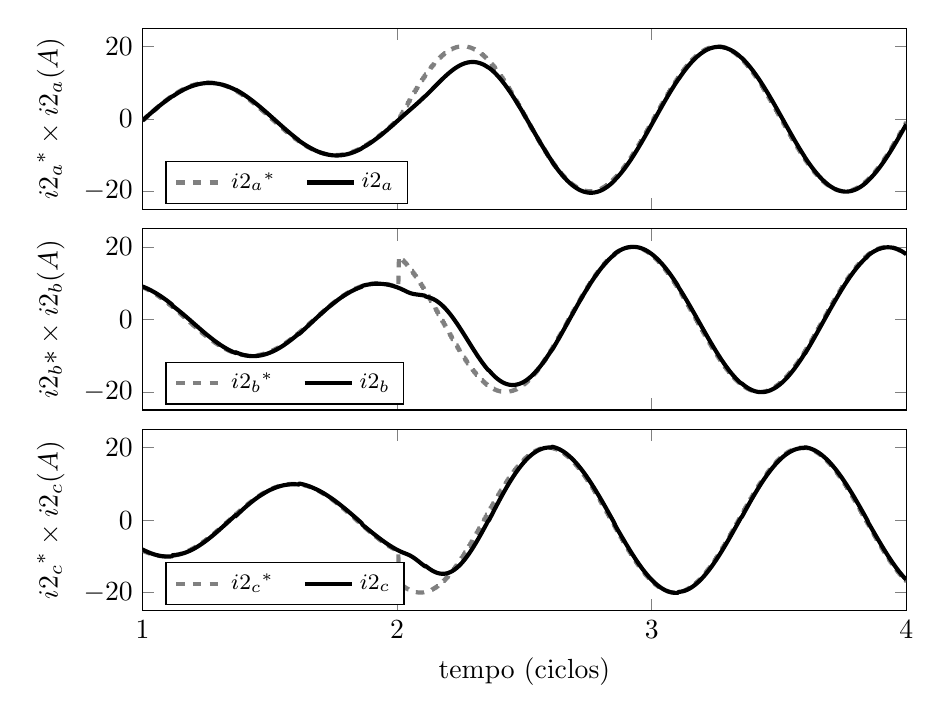
\begin{tikzpicture}

\begin{axis}[%
width=0.8\textwidth,
height=0.189701500343624\textwidth,
scale only axis,
xmin=0.0166666666666667,
xmax=0.0666666666666667,
xtick={0.0166666666666667,0.0333333333333333,0.05,0.0666666666666667},
xticklabels={\empty},
ymin=-25,
ymax=25,
ytick={-20,   0,  20},
ylabel={${\text{i2}_\text{b}}\text{* }\times\text{ i2}_\text{b}\text{ (A)}$},
name=plot2,
legend style={at={(0.03,0.03)},anchor=south west,draw=black,fill=white,legend cell align=left},
scaled x ticks = false,
legend columns=-1,
legend style={/tikz/every even column/.append style={column sep=0.3cm}},
legend style={font=\footnotesize}
]
\addplot [color=gray,dashed,line width=1.5pt]
  table[row sep=crcr]{0.0166583333333333	8.95711760239421\\
0.0167	8.81303452065\\
0.0167416666666667	8.81303452065\\
0.0167833333333333	8.66025403784447\\
0.016825	8.66025403784447\\
0.0168666666666667	8.49892692986872\\
0.0169083333333333	8.49892692986872\\
0.01695	8.32921240710107\\
0.0169916666666667	8.32921240710107\\
0.0170333333333333	8.15127795728562\\
0.017075	8.15127795728562\\
0.0171166666666667	7.96529918024204\\
0.0171583333333333	7.96529918024204\\
0.0172	7.77145961456979\\
0.0172416666666667	7.77145961456979\\
0.0172833333333333	7.56995055651764\\
0.017325	7.56995055651764\\
0.0173666666666667	7.36097087119742\\
0.0174083333333333	7.36097087119742\\
0.01745	7.1447267963281\\
0.0174916666666667	7.1447267963281\\
0.0175333333333333	6.92143173870414\\
0.017575	6.92143173870414\\
0.0176166666666667	6.69130606358865\\
0.0176583333333333	6.69130606358865\\
0.0177	6.45457687723957\\
0.0177416666666667	6.45457687723957\\
0.0177833333333333	6.21147780278317\\
0.017825	6.21147780278317\\
0.0178666666666667	5.96224874965622\\
0.0179083333333333	5.96224874965622\\
0.01795	5.70713567684438\\
0.0179916666666667	5.70713567684438\\
0.0180333333333333	5.44639035015033\\
0.018075	5.44639035015033\\
0.0181166666666667	5.18027009373136\\
0.0181583333333333	5.18027009373136\\
0.0182	4.90903753615147\\
0.0182416666666667	4.90903753615147\\
0.0182833333333333	4.63296035119867\\
0.018325	4.63296035119867\\
0.0183666666666667	4.35231099372333\\
0.0184083333333333	4.35231099372333\\
0.01845	4.06736643075805\\
0.0184916666666667	4.06736643075805\\
0.0185333333333333	3.77840786818472\\
0.018575	3.77840786818472\\
0.0186166666666667	3.4857204732182\\
0.0186583333333333	3.4857204732182\\
0.0187	3.18959309298074\\
0.0187416666666667	3.18959309298074\\
0.0187833333333333	2.89031796944476\\
0.018825	2.89031796944476\\
0.0188666666666667	2.58819045102524\\
0.0189083333333333	2.58819045102524\\
0.01895	2.28350870110659\\
0.0189916666666667	2.28350870110659\\
0.0190333333333333	1.97657340379129\\
0.019075	1.97657340379129\\
0.0191166666666667	1.66768746716105\\
0.0191583333333333	1.66768746716105\\
0.0192	1.35715572434307\\
0.0192416666666667	1.35715572434307\\
0.0192833333333333	1.04528463267656\\
0.019325	1.04528463267656\\
0.0193666666666667	0.732381971276336\\
0.0194083333333333	0.732381971276336\\
0.01945	0.418756537292012\\
0.0194916666666667	0.418756537292012\\
0.0195333333333333	0.104717841162471\\
0.019575	0.104717841162471\\
0.0196166666666667	-0.20942419883356\\
0.0196583333333333	-0.20942419883356\\
0.0197	-0.523359562429432\\
0.0197416666666667	-0.523359562429432\\
0.0197833333333333	-0.836778433323152\\
0.019825	-0.836778433323152\\
0.0198666666666667	-1.14937150492867\\
0.0199083333333333	-1.14937150492867\\
0.01995	-1.46083028562412\\
0.0199916666666667	-1.46083028562412\\
0.0200333333333333	-1.77084740319584\\
0.020075	-1.77084740319584\\
0.0201166666666667	-2.0791169081776\\
0.0201583333333333	-2.0791169081776\\
0.0202	-2.38533457578582\\
0.0202416666666667	-2.38533457578582\\
0.0202833333333333	-2.68919820615267\\
0.020325	-2.68919820615267\\
0.0203666666666667	-2.99040792256089\\
0.0204083333333333	-2.99040792256089\\
0.02045	-3.28866646738586\\
0.0204916666666667	-3.28866646738586\\
0.0205333333333333	-3.58367949545303\\
0.020575	-3.58367949545303\\
0.0206166666666667	-3.87515586452106\\
0.0206583333333333	-3.87515586452106\\
0.0207	-4.16280792260405\\
0.0207416666666667	-4.16280792260405\\
0.0207833333333333	-4.44635179184931\\
0.020825	-4.44635179184931\\
0.0208666666666667	-4.72550764869058\\
0.0209083333333333	-4.72550764869058\\
0.02095	-5.00000000000005\\
0.0209916666666667	-5.00000000000005\\
0.0210333333333333	-5.26955795496682\\
0.021075	-5.26955795496682\\
0.0211166666666667	-5.53391549243349\\
0.0211583333333333	-5.53391549243349\\
0.0212	-5.79281172342684\\
0.0212416666666667	-5.79281172342684\\
0.0212833333333333	-6.0459911486238\\
0.021325	-6.0459911486238\\
0.0213666666666667	-6.29320391049844\\
0.0214083333333333	-6.29320391049844\\
0.02145	-6.53420603990112\\
0.0214916666666667	-6.53420603990112\\
0.0215333333333333	-6.76875969682667\\
0.021575	-6.76875969682667\\
0.0216166666666667	-6.99663340513372\\
0.0216583333333333	-6.99663340513372\\
0.0217	-7.2176022809837\\
0.0217416666666667	-7.2176022809837\\
0.0217833333333333	-7.43144825477402\\
0.021825	-7.43144825477402\\
0.0218666666666667	-7.6379602863465\\
0.0219083333333333	-7.6379602863465\\
0.02195	-7.83693457325848\\
0.0219916666666667	-7.83693457325848\\
0.0220333333333333	-8.02817475191123\\
0.022075	-8.02817475191123\\
0.0221166666666667	-8.21149209133713\\
0.0221583333333333	-8.21149209133713\\
0.0222	-8.38670567945433\\
0.0222416666666667	-8.38670567945433\\
0.0222833333333333	-8.55364260160516\\
0.022325	-8.55364260160516\\
0.0223666666666667	-8.71213811120199\\
0.0224083333333333	-8.71213811120199\\
0.02245	-8.86203579231225\\
0.0224916666666667	-8.86203579231225\\
0.0225333333333333	-9.00318771402204\\
0.022575	-9.00318771402204\\
0.0226166666666667	-9.13545457642611\\
0.0226583333333333	-9.13545457642611\\
0.0227	-9.25870584810006\\
0.0227416666666667	-9.25870584810006\\
0.0227833333333333	-9.37281989491902\\
0.022825	-9.37281989491902\\
0.0228666666666667	-9.47768410009597\\
0.0229083333333333	-9.47768410009597\\
0.02295	-9.57319497532079\\
0.0229916666666667	-9.57319497532079\\
0.0230333333333333	-9.6592582628908\\
0.023075	-9.6592582628908\\
0.0231166666666667	-9.73578902873172\\
0.0231583333333333	-9.73578902873172\\
0.0232	-9.80271174621734\\
0.0232416666666667	-9.80271174621734\\
0.0232833333333333	-9.85996037070517\\
0.023325	-9.85996037070517\\
0.0233666666666667	-9.90747840471456\\
0.0234083333333333	-9.90747840471456\\
0.02345	-9.94521895368285\\
0.0234916666666667	-9.94521895368285\\
0.0235333333333333	-9.97314477224471\\
0.023575	-9.97314477224471\\
0.0236166666666667	-9.99122830098871\\
0.0236583333333333	-9.99122830098871\\
0.0237	-9.99945169365525\\
0.0237416666666667	-9.99945169365525\\
0.0237833333333333	-9.99780683474858\\
0.023825	-9.99780683474858\\
0.0238666666666667	-9.98629534754587\\
0.0239083333333333	-9.98629534754587\\
0.02395	-9.96492859249517\\
0.0239916666666667	-9.96492859249517\\
0.0240333333333333	-9.93372765600409\\
0.024075	-9.93372765600409\\
0.0241166666666667	-9.89272332963001\\
0.0241583333333333	-9.89272332963001\\
0.0242	-9.84195607969255\\
0.0242416666666667	-9.84195607969255\\
0.0242833333333333	-9.78147600733818\\
0.024325	-9.78147600733818\\
0.0243666666666667	-9.71134279909649\\
0.0244083333333333	-9.71134279909649\\
0.02445	-9.63162566797671\\
0.0244916666666667	-9.63162566797671\\
0.0245333333333333	-9.5424032851629\\
0.024575	-9.5424032851629\\
0.0246166666666667	-9.44376370237494\\
0.0246583333333333	-9.44376370237494\\
0.0247	-9.33580426497215\\
0.0247416666666667	-9.33580426497215\\
0.0247833333333333	-9.21863151588513\\
0.024825	-9.21863151588513\\
0.0248666666666667	-9.09236109047081\\
0.0249083333333333	-9.09236109047081\\
0.02495	-8.95711760239425\\
0.0249916666666667	-8.95711760239425\\
0.0250333333333333	-8.81303452065005\\
0.025075	-8.81303452065005\\
0.0251166666666667	-8.66025403784451\\
0.0251583333333333	-8.66025403784451\\
0.0252	-8.49892692986876\\
0.0252416666666667	-8.49892692986876\\
0.0252833333333333	-8.32921240710111\\
0.025325	-8.32921240710111\\
0.0253666666666667	-8.15127795728566\\
0.0254083333333333	-8.15127795728566\\
0.02545	-7.96529918024207\\
0.0254916666666667	-7.96529918024207\\
0.0255333333333333	-7.77145961456982\\
0.025575	-7.77145961456982\\
0.0256166666666667	-7.56995055651767\\
0.0256583333333333	-7.56995055651767\\
0.0257	-7.36097087119745\\
0.0257416666666667	-7.36097087119745\\
0.0257833333333333	-7.14472679632814\\
0.025825	-7.14472679632814\\
0.0258666666666667	-6.92143173870417\\
0.0259083333333333	-6.92143173870417\\
0.02595	-6.69130606358868\\
0.0259916666666667	-6.69130606358868\\
0.0260333333333333	-6.4545768772396\\
0.026075	-6.4545768772396\\
0.0261166666666667	-6.2114778027832\\
0.0261583333333333	-6.2114778027832\\
0.0262	-5.96224874965625\\
0.0262416666666667	-5.96224874965625\\
0.0262833333333333	-5.70713567684441\\
0.026325	-5.70713567684441\\
0.0263666666666667	-5.44639035015036\\
0.0264083333333333	-5.44639035015036\\
0.02645	-5.18027009373139\\
0.0264916666666667	-5.18027009373139\\
0.0265333333333333	-4.90903753615149\\
0.026575	-4.90903753615149\\
0.0266166666666667	-4.6329603511987\\
0.0266583333333333	-4.6329603511987\\
0.0267	-4.35231099372335\\
0.0267416666666667	-4.35231099372335\\
0.0267833333333333	-4.06736643075807\\
0.026825	-4.06736643075807\\
0.0268666666666667	-3.77840786818474\\
0.0269083333333333	-3.77840786818474\\
0.02695	-3.48572047321821\\
0.0269916666666667	-3.48572047321821\\
0.0270333333333333	-3.18959309298076\\
0.027075	-3.18959309298076\\
0.0271166666666667	-2.89031796944477\\
0.0271583333333333	-2.89031796944477\\
0.0272	-2.58819045102526\\
0.0272416666666667	-2.58819045102526\\
0.0272833333333333	-2.28350870110661\\
0.027325	-2.28350870110661\\
0.0273666666666667	-1.9765734037913\\
0.0274083333333333	-1.9765734037913\\
0.02745	-1.66768746716106\\
0.0274916666666667	-1.66768746716106\\
0.0275333333333333	-1.35715572434308\\
0.027575	-1.35715572434308\\
0.0276166666666667	-1.04528463267656\\
0.0276583333333333	-1.04528463267656\\
0.0277	-0.732381971276341\\
0.0277416666666667	-0.732381971276341\\
0.0277833333333333	-0.418756537292015\\
0.027825	-0.418756537292015\\
0.0278666666666667	-0.104717841162473\\
0.0279083333333333	-0.104717841162473\\
0.02795	0.209424198833559\\
0.0279916666666667	0.209424198833559\\
0.0280333333333333	0.523359562429433\\
0.028075	0.523359562429433\\
0.0281166666666667	0.836778433323154\\
0.0281583333333333	0.836778433323154\\
0.0282	1.14937150492867\\
0.0282416666666667	1.14937150492867\\
0.0282833333333333	1.46083028562412\\
0.028325	1.46083028562412\\
0.0283666666666667	1.77084740319585\\
0.0284083333333333	1.77084740319585\\
0.02845	2.07911690817761\\
0.0284916666666667	2.07911690817761\\
0.0285333333333333	2.38533457578583\\
0.028575	2.38533457578583\\
0.0286166666666667	2.68919820615268\\
0.0286583333333333	2.68919820615268\\
0.0287	2.9904079225609\\
0.0287416666666667	2.9904079225609\\
0.0287833333333333	3.28866646738587\\
0.028825	3.28866646738587\\
0.0288666666666667	3.58367949545304\\
0.0289083333333333	3.58367949545304\\
0.02895	3.87515586452107\\
0.0289916666666667	3.87515586452107\\
0.0290333333333333	4.16280792260406\\
0.029075	4.16280792260406\\
0.0291166666666667	4.44635179184933\\
0.0291583333333333	4.44635179184933\\
0.0292	4.7255076486906\\
0.0292416666666667	4.7255076486906\\
0.0292833333333333	5.00000000000006\\
0.029325	5.00000000000006\\
0.0293666666666667	5.26955795496684\\
0.0294083333333333	5.26955795496684\\
0.02945	5.53391549243351\\
0.0294916666666667	5.53391549243351\\
0.0295333333333333	5.79281172342686\\
0.029575	5.79281172342686\\
0.0296166666666667	6.04599114862383\\
0.0296583333333333	6.04599114862383\\
0.0297	6.29320391049846\\
0.0297416666666667	6.29320391049846\\
0.0297833333333333	6.53420603990114\\
0.029825	6.53420603990114\\
0.0298666666666667	6.7687596968267\\
0.0299083333333333	6.7687596968267\\
0.02995	6.99663340513375\\
0.0299916666666667	6.99663340513375\\
0.0300333333333333	7.21760228098372\\
0.030075	7.21760228098372\\
0.0301166666666667	7.43144825477405\\
0.0301583333333333	7.43144825477405\\
0.0302	7.63796028634653\\
0.0302416666666667	7.63796028634653\\
0.0302833333333333	7.83693457325851\\
0.030325	7.83693457325851\\
0.0303666666666667	8.02817475191126\\
0.0304083333333333	8.02817475191126\\
0.03045	8.21149209133716\\
0.0304916666666667	8.21149209133716\\
0.0305333333333333	8.38670567945436\\
0.030575	8.38670567945436\\
0.0306166666666667	8.55364260160519\\
0.0306583333333333	8.55364260160519\\
0.0307	8.71213811120203\\
0.0307416666666667	8.71213811120203\\
0.0307833333333333	8.86203579231228\\
0.030825	8.86203579231228\\
0.0308666666666667	9.00318771402207\\
0.0309083333333333	9.00318771402207\\
0.03095	9.13545457642615\\
0.0309916666666667	9.13545457642615\\
0.0310333333333333	9.25870584810009\\
0.031075	9.25870584810009\\
0.0311166666666667	9.37281989491906\\
0.0311583333333333	9.37281989491906\\
0.0312	9.477684100096\\
0.0312416666666667	9.477684100096\\
0.0312833333333333	9.57319497532082\\
0.031325	9.57319497532082\\
0.0313666666666667	9.65925826289084\\
0.0314083333333333	9.65925826289084\\
0.03145	9.73578902873176\\
0.0314916666666667	9.73578902873176\\
0.0315333333333333	9.80271174621738\\
0.031575	9.80271174621738\\
0.0316166666666667	9.85996037070521\\
0.0316583333333333	9.85996037070521\\
0.0317	9.9074784047146\\
0.0317416666666667	9.9074784047146\\
0.0317833333333333	9.94521895368289\\
0.031825	9.94521895368289\\
0.0318666666666667	9.97314477224474\\
0.0319083333333333	9.97314477224474\\
0.03195	9.99122830098875\\
0.0319916666666667	9.99122830098875\\
0.0320333333333333	9.99945169365528\\
0.032075	9.99945169365528\\
0.0321166666666667	9.99780683474862\\
0.0321583333333333	9.99780683474862\\
0.0322	9.98629534754591\\
0.0322416666666667	9.98629534754591\\
0.0322833333333333	9.96492859249521\\
0.032325	9.96492859249521\\
0.0323666666666667	9.93372765600413\\
0.0324083333333333	9.93372765600413\\
0.03245	9.89272332963005\\
0.0324916666666667	9.89272332963005\\
0.0325333333333333	9.84195607969259\\
0.032575	9.84195607969259\\
0.0326166666666667	9.78147600733822\\
0.0326583333333333	9.78147600733822\\
0.0327	9.71134279909653\\
0.0327416666666667	9.71134279909653\\
0.0327833333333333	9.63162566797675\\
0.032825	9.63162566797675\\
0.0328666666666667	9.54240328516294\\
0.0329083333333333	9.54240328516294\\
0.03295	9.44376370237498\\
0.0329916666666667	9.44376370237498\\
0.0330333333333333	9.33580426497218\\
0.033075	9.33580426497218\\
0.0331166666666667	9.21863151588517\\
0.0331583333333333	9.21863151588517\\
0.0332	9.09236109047085\\
0.0332416666666667	9.09236109047085\\
0.0332833333333333	8.95711760239429\\
0.033325	8.95711760239429\\
0.0333666666666667	8.81303452065008\\
0.0334083333333333	8.81303452065008\\
0.03345	17.3205080756891\\
0.0334916666666667	17.3205080756891\\
0.0335333333333333	16.9978538597376\\
0.033575	16.9978538597376\\
0.0336166666666667	16.6584248142023\\
0.0336583333333333	16.6584248142023\\
0.0337	16.3025559145714\\
0.0337416666666667	16.3025559145714\\
0.0337833333333333	15.9305983604842\\
0.033825	15.9305983604842\\
0.0338666666666667	15.5429192291397\\
0.0339083333333333	15.5429192291397\\
0.03395	15.1399011130354\\
0.0339916666666667	15.1399011130354\\
0.0340333333333333	14.721941742395\\
0.034075	14.721941742395\\
0.0341166666666667	14.2894535926563\\
0.0341583333333333	14.2894535926563\\
0.0342	13.8428634774084\\
0.0342416666666667	13.8428634774084\\
0.0342833333333333	13.3826121271774\\
0.034325	13.3826121271774\\
0.0343666666666667	12.9091537544793\\
0.0344083333333333	12.9091537544793\\
0.03445	12.4229556055665\\
0.0344916666666667	12.4229556055665\\
0.0345333333333333	11.9244974993126\\
0.034575	11.9244974993126\\
0.0346166666666667	11.4142713536889\\
0.0346583333333333	11.4142713536889\\
0.0347	10.8927807003008\\
0.0347416666666667	10.8927807003008\\
0.0347833333333333	10.3605401874628\\
0.034825	10.3605401874628\\
0.0348666666666667	9.81807507230302\\
0.0349083333333333	9.81807507230302\\
0.03495	9.26592070239743\\
0.0349916666666667	9.26592070239743\\
0.0350333333333333	8.70462198744674\\
0.035075	8.70462198744674\\
0.0351166666666667	8.13473286151618\\
0.0351583333333333	8.13473286151618\\
0.0352	7.55681573636951\\
0.0352416666666667	7.55681573636951\\
0.0352833333333333	6.97144094643646\\
0.035325	6.97144094643646\\
0.0353666666666667	6.37918618596155\\
0.0354083333333333	6.37918618596155\\
0.03545	5.78063593888957\\
0.0354916666666667	5.78063593888957\\
0.0355333333333333	5.17638090205054\\
0.035575	5.17638090205054\\
0.0356166666666667	4.56701740221323\\
0.0356583333333333	4.56701740221323\\
0.0357	3.95314680758263\\
0.0357416666666667	3.95314680758263\\
0.0357833333333333	3.33537493432214\\
0.035825	3.33537493432214\\
0.0358666666666667	2.71431144868617\\
0.0359083333333333	2.71431144868617\\
0.03595	2.09056926535314\\
0.0359916666666667	2.09056926535314\\
0.0360333333333333	1.4647639425527\\
0.036075	1.4647639425527\\
0.0361166666666667	0.837513074584043\\
0.0361583333333333	0.837513074584043\\
0.0362	0.209435682324955\\
0.0362416666666667	0.209435682324955\\
0.0362833333333333	-0.418848397667113\\
0.036325	-0.418848397667113\\
0.0363666666666667	-1.04671912485886\\
0.0364083333333333	-1.04671912485886\\
0.03645	-1.67355686664631\\
0.0364916666666667	-1.67355686664631\\
0.0365333333333333	-2.29874300985734\\
0.036575	-2.29874300985734\\
0.0366166666666667	-2.92166057124825\\
0.0366583333333333	-2.92166057124825\\
0.0367	-3.5416948063917\\
0.0367416666666667	-3.5416948063917\\
0.0367833333333333	-4.15823381635523\\
0.036825	-4.15823381635523\\
0.0368666666666667	-4.77066915157168\\
0.0369083333333333	-4.77066915157168\\
0.03695	-5.37839641230538\\
0.0369916666666667	-5.37839641230538\\
0.0370333333333333	-5.98081584512182\\
0.037075	-5.98081584512182\\
0.0371166666666667	-6.57733293477176\\
0.0371583333333333	-6.57733293477176\\
0.0372	-7.16735899090611\\
0.0372416666666667	-7.16735899090611\\
0.0372833333333333	-7.75031172904218\\
0.037325	-7.75031172904218\\
0.0373666666666667	-8.32561584520815\\
0.0374083333333333	-8.32561584520815\\
0.03745	-8.89270358369869\\
0.0374916666666667	-8.89270358369869\\
0.0375333333333333	-9.45101529738123\\
0.037575	-9.45101529738123\\
0.0376166666666667	-10.0000000000002\\
0.0376583333333333	-10.0000000000002\\
0.0377	-10.5391159099337\\
0.0377416666666667	-10.5391159099337\\
0.0377833333333333	-11.0678309848671\\
0.037825	-11.0678309848671\\
0.0378666666666667	-11.5856234468538\\
0.0379083333333333	-11.5856234468538\\
0.03795	-12.0919822972477\\
0.0379916666666667	-12.0919822972477\\
0.0380333333333333	-12.586407820997\\
0.038075	-12.586407820997\\
0.0381166666666667	-13.0684120798023\\
0.0381583333333333	-13.0684120798023\\
0.0382	-13.5375193936535\\
0.0382416666666667	-13.5375193936535\\
0.0382833333333333	-13.9932668102676\\
0.038325	-13.9932668102676\\
0.0383666666666667	-14.4352045619675\\
0.0384083333333333	-14.4352045619675\\
0.03845	-14.8628965095482\\
0.0384916666666667	-14.8628965095482\\
0.0385333333333333	-15.2759205726931\\
0.038575	-15.2759205726931\\
0.0386166666666667	-15.6738691465171\\
0.0386583333333333	-15.6738691465171\\
0.0387	-16.0563495038226\\
0.0387416666666667	-16.0563495038226\\
0.0387833333333333	-16.4229841826744\\
0.038825	-16.4229841826744\\
0.0388666666666667	-16.7734113589088\\
0.0389083333333333	-16.7734113589088\\
0.03895	-17.1072852032105\\
0.0389916666666667	-17.1072852032105\\
0.0390333333333333	-17.4242762224041\\
0.039075	-17.4242762224041\\
0.0391166666666667	-17.7240715846246\\
0.0391583333333333	-17.7240715846246\\
0.0392	-18.0063754280442\\
0.0392416666666667	-18.0063754280442\\
0.0392833333333333	-18.2709091528524\\
0.039325	-18.2709091528524\\
0.0393666666666667	-18.5174116962003\\
0.0394083333333333	-18.5174116962003\\
0.03945	-18.7456397898382\\
0.0394916666666667	-18.7456397898382\\
0.0395333333333333	-18.9553682001921\\
0.039575	-18.9553682001921\\
0.0396166666666667	-19.1463899506417\\
0.0396583333333333	-19.1463899506417\\
0.0397	-19.3185165257817\\
0.0397416666666667	-19.3185165257817\\
0.0397833333333333	-19.4715780574636\\
0.039825	-19.4715780574636\\
0.0398666666666667	-19.6054234924348\\
0.0399083333333333	-19.6054234924348\\
0.03995	-19.7199207414105\\
0.0399916666666667	-19.7199207414105\\
0.0400333333333333	-19.8149568094293\\
0.040075	-19.8149568094293\\
0.0401166666666667	-19.8904379073659\\
0.0401583333333333	-19.8904379073659\\
0.0402	-19.9462895444896\\
0.0402416666666667	-19.9462895444896\\
0.0402833333333333	-19.9824566019776\\
0.040325	-19.9824566019776\\
0.0403666666666667	-19.9989033873107\\
0.0404083333333333	-19.9989033873107\\
0.04045	-19.9956136694973\\
0.0404916666666667	-19.9956136694973\\
0.0405333333333333	-19.9725906950919\\
0.040575	-19.9725906950919\\
0.0406166666666667	-19.9298571849905\\
0.0406583333333333	-19.9298571849905\\
0.0407	-19.8674553120083\\
0.0407416666666667	-19.8674553120083\\
0.0407833333333333	-19.7854466592602\\
0.040825	-19.7854466592602\\
0.0408666666666667	-19.6839121593853\\
0.0409083333333333	-19.6839121593853\\
0.04095	-19.5629520146765\\
0.0409916666666667	-19.5629520146765\\
0.0410333333333333	-19.4226855981931\\
0.041075	-19.4226855981931\\
0.0411166666666667	-19.2632513359536\\
0.0411583333333333	-19.2632513359536\\
0.0412	-19.084806570326\\
0.0412416666666667	-19.084806570326\\
0.0412833333333333	-18.88752740475\\
0.041325	-18.88752740475\\
0.0413666666666667	-18.6716085299444\\
0.0414083333333333	-18.6716085299444\\
0.04145	-18.4372630317704\\
0.0414916666666667	-18.4372630317704\\
0.0415333333333333	-18.1847221809418\\
0.041575	-18.1847221809418\\
0.0416166666666667	-17.9142352047887\\
0.0416583333333333	-17.9142352047887\\
0.0417	-17.6260690413002\\
0.0417416666666667	-17.6260690413002\\
0.0417833333333333	-17.3205080756892\\
0.041825	-17.3205080756892\\
0.0418666666666667	-16.9978538597377\\
0.0419083333333333	-16.9978538597377\\
0.04195	-16.6584248142024\\
0.0419916666666667	-16.6584248142024\\
0.0420333333333333	-16.3025559145715\\
0.042075	-16.3025559145715\\
0.0421166666666667	-15.9305983604843\\
0.0421583333333333	-15.9305983604843\\
0.0422	-15.5429192291398\\
0.0422416666666667	-15.5429192291398\\
0.0422833333333333	-15.1399011130355\\
0.042325	-15.1399011130355\\
0.0423666666666667	-14.721941742395\\
0.0424083333333333	-14.721941742395\\
0.04245	-14.2894535926564\\
0.0424916666666667	-14.2894535926564\\
0.0425333333333333	-13.8428634774085\\
0.042575	-13.8428634774085\\
0.0426166666666667	-13.3826121271775\\
0.0426583333333333	-13.3826121271775\\
0.0427	-12.9091537544793\\
0.0427416666666667	-12.9091537544793\\
0.0427833333333333	-12.4229556055665\\
0.042825	-12.4229556055665\\
0.0428666666666667	-11.9244974993126\\
0.0429083333333333	-11.9244974993126\\
0.04295	-11.4142713536889\\
0.0429916666666667	-11.4142713536889\\
0.0430333333333333	-10.8927807003008\\
0.043075	-10.8927807003008\\
0.0431166666666667	-10.3605401874629\\
0.0431583333333333	-10.3605401874629\\
0.0432	-9.81807507230306\\
0.0432416666666667	-9.81807507230306\\
0.0432833333333333	-9.26592070239747\\
0.043325	-9.26592070239747\\
0.0433666666666667	-8.70462198744678\\
0.0434083333333333	-8.70462198744678\\
0.04345	-8.13473286151622\\
0.0434916666666667	-8.13473286151622\\
0.0435333333333333	-7.55681573636955\\
0.043575	-7.55681573636955\\
0.0436166666666667	-6.97144094643649\\
0.0436583333333333	-6.97144094643649\\
0.0437	-6.37918618596158\\
0.0437416666666667	-6.37918618596158\\
0.0437833333333333	-5.7806359388896\\
0.043825	-5.7806359388896\\
0.0438666666666667	-5.17638090205057\\
0.0439083333333333	-5.17638090205057\\
0.04395	-4.56701740221326\\
0.0439916666666667	-4.56701740221326\\
0.0440333333333333	-3.95314680758265\\
0.044075	-3.95314680758265\\
0.0441166666666667	-3.33537493432216\\
0.0441583333333333	-3.33537493432216\\
0.0442	-2.71431144868619\\
0.0442416666666667	-2.71431144868619\\
0.0442833333333333	-2.09056926535316\\
0.044325	-2.09056926535316\\
0.0443666666666667	-1.46476394255271\\
0.0444083333333333	-1.46476394255271\\
0.04445	-0.83751307458405\\
0.0444916666666667	-0.83751307458405\\
0.0445333333333333	-0.209435682324959\\
0.044575	-0.209435682324959\\
0.0446166666666667	0.418848397667111\\
0.0446583333333333	0.418848397667111\\
0.0447	1.04671912485886\\
0.0447416666666667	1.04671912485886\\
0.0447833333333333	1.67355686664631\\
0.044825	1.67355686664631\\
0.0448666666666667	2.29874300985735\\
0.0449083333333333	2.29874300985735\\
0.04495	2.92166057124826\\
0.0449916666666667	2.92166057124826\\
0.0450333333333333	3.54169480639171\\
0.045075	3.54169480639171\\
0.0451166666666667	4.15823381635525\\
0.0451583333333333	4.15823381635525\\
0.0452	4.77066915157169\\
0.0452416666666667	4.77066915157169\\
0.0452833333333333	5.37839641230541\\
0.045325	5.37839641230541\\
0.0453666666666667	5.98081584512184\\
0.0454083333333333	5.98081584512184\\
0.04545	6.57733293477179\\
0.0454916666666667	6.57733293477179\\
0.0455333333333333	7.16735899090614\\
0.045575	7.16735899090614\\
0.0456166666666667	7.75031172904221\\
0.0456583333333333	7.75031172904221\\
0.0457	8.32561584520819\\
0.0457416666666667	8.32561584520819\\
0.0457833333333333	8.89270358369873\\
0.045825	8.89270358369873\\
0.0458666666666667	9.45101529738127\\
0.0459083333333333	9.45101529738127\\
0.04595	10.0000000000002\\
0.0459916666666667	10.0000000000002\\
0.0460333333333333	10.5391159099338\\
0.046075	10.5391159099338\\
0.0461166666666667	11.0678309848671\\
0.0461583333333333	11.0678309848671\\
0.0462	11.5856234468538\\
0.0462416666666667	11.5856234468538\\
0.0462833333333333	12.0919822972478\\
0.046325	12.0919822972478\\
0.0463666666666667	12.586407820997\\
0.0464083333333333	12.586407820997\\
0.04645	13.0684120798024\\
0.0464916666666667	13.0684120798024\\
0.0465333333333333	13.5375193936535\\
0.046575	13.5375193936535\\
0.0466166666666667	13.9932668102676\\
0.0466583333333333	13.9932668102676\\
0.0467	14.4352045619676\\
0.0467416666666667	14.4352045619676\\
0.0467833333333333	14.8628965095482\\
0.046825	14.8628965095482\\
0.0468666666666667	15.2759205726932\\
0.0469083333333333	15.2759205726932\\
0.04695	15.6738691465172\\
0.0469916666666667	15.6738691465172\\
0.0470333333333333	16.0563495038227\\
0.047075	16.0563495038227\\
0.0471166666666667	16.4229841826745\\
0.0471583333333333	16.4229841826745\\
0.0472	16.7734113589089\\
0.0472416666666667	16.7734113589089\\
0.0472833333333333	17.1072852032105\\
0.047325	17.1072852032105\\
0.0473666666666667	17.4242762224042\\
0.0474083333333333	17.4242762224042\\
0.04745	17.7240715846247\\
0.0474916666666667	17.7240715846247\\
0.0475333333333333	18.0063754280443\\
0.047575	18.0063754280443\\
0.0476166666666667	18.2709091528525\\
0.0476583333333333	18.2709091528525\\
0.0477	18.5174116962003\\
0.0477416666666667	18.5174116962003\\
0.0477833333333333	18.7456397898383\\
0.047825	18.7456397898383\\
0.0478666666666667	18.9553682001922\\
0.0479083333333333	18.9553682001922\\
0.04795	19.1463899506418\\
0.0479916666666667	19.1463899506418\\
0.0480333333333333	19.3185165257818\\
0.048075	19.3185165257818\\
0.0481166666666667	19.4715780574637\\
0.0481583333333333	19.4715780574637\\
0.0482	19.6054234924349\\
0.0482416666666667	19.6054234924349\\
0.0482833333333333	19.7199207414106\\
0.048325	19.7199207414106\\
0.0483666666666667	19.8149568094294\\
0.0484083333333333	19.8149568094294\\
0.04845	19.890437907366\\
0.0484916666666667	19.890437907366\\
0.0485333333333333	19.9462895444897\\
0.048575	19.9462895444897\\
0.0486166666666667	19.9824566019777\\
0.0486583333333333	19.9824566019777\\
0.0487	19.9989033873107\\
0.0487416666666667	19.9989033873107\\
0.0487833333333333	19.9956136694974\\
0.048825	19.9956136694974\\
0.0488666666666667	19.972590695092\\
0.0489083333333333	19.972590695092\\
0.04895	19.9298571849906\\
0.0489916666666667	19.9298571849906\\
0.0490333333333333	19.8674553120084\\
0.049075	19.8674553120084\\
0.0491166666666667	19.7854466592603\\
0.0491583333333333	19.7854466592603\\
0.0492	19.6839121593854\\
0.0492416666666667	19.6839121593854\\
0.0492833333333333	19.5629520146766\\
0.049325	19.5629520146766\\
0.0493666666666667	19.4226855981932\\
0.0494083333333333	19.4226855981932\\
0.04945	19.2632513359537\\
0.0494916666666667	19.2632513359537\\
0.0495333333333333	19.084806570326\\
0.049575	19.084806570326\\
0.0496166666666667	18.8875274047501\\
0.0496583333333333	18.8875274047501\\
0.0497	18.6716085299445\\
0.0497416666666667	18.6716085299445\\
0.0497833333333333	18.4372630317705\\
0.049825	18.4372630317705\\
0.0498666666666667	18.1847221809419\\
0.0499083333333333	18.1847221809419\\
0.04995	17.9142352047887\\
0.0499916666666667	17.9142352047887\\
0.0500333333333333	17.6260690413003\\
0.050075	17.6260690413003\\
0.0501166666666667	17.3205080756892\\
0.0501583333333333	17.3205080756892\\
0.0502	16.9978538597377\\
0.0502416666666667	16.9978538597377\\
0.0502833333333333	16.6584248142025\\
0.050325	16.6584248142025\\
0.0503666666666667	16.3025559145715\\
0.0504083333333333	16.3025559145715\\
0.05045	15.9305983604844\\
0.0504916666666667	15.9305983604844\\
0.0505333333333333	15.5429192291399\\
0.050575	15.5429192291399\\
0.0506166666666667	15.1399011130356\\
0.0506583333333333	15.1399011130356\\
0.0507	14.7219417423951\\
0.0507416666666667	14.7219417423951\\
0.0507833333333333	14.2894535926565\\
0.050825	14.2894535926565\\
0.0508666666666667	13.8428634774085\\
0.0509083333333333	13.8428634774085\\
0.05095	13.3826121271776\\
0.0509916666666667	13.3826121271776\\
0.0510333333333333	12.9091537544794\\
0.051075	12.9091537544794\\
0.0511166666666667	12.4229556055666\\
0.0511583333333333	12.4229556055666\\
0.0512	11.9244974993127\\
0.0512416666666667	11.9244974993127\\
0.0512833333333333	11.414271353689\\
0.051325	11.414271353689\\
0.0513666666666667	10.8927807003009\\
0.0514083333333333	10.8927807003009\\
0.05145	10.3605401874629\\
0.0514916666666667	10.3605401874629\\
0.0515333333333333	9.81807507230311\\
0.051575	9.81807507230311\\
0.0516166666666667	9.26592070239752\\
0.0516583333333333	9.26592070239752\\
0.0517	8.70462198744682\\
0.0517416666666667	8.70462198744682\\
0.0517833333333333	8.13473286151626\\
0.051825	8.13473286151626\\
0.0518666666666667	7.55681573636959\\
0.0519083333333333	7.55681573636959\\
0.05195	6.97144094643653\\
0.0519916666666667	6.97144094643653\\
0.0520333333333333	6.37918618596161\\
0.052075	6.37918618596161\\
0.0521166666666667	5.78063593888963\\
0.0521583333333333	5.78063593888963\\
0.0522	5.1763809020506\\
0.0522416666666667	5.1763809020506\\
0.0522833333333333	4.56701740221328\\
0.052325	4.56701740221328\\
0.0523666666666667	3.95314680758267\\
0.0524083333333333	3.95314680758267\\
0.05245	3.33537493432218\\
0.0524916666666667	3.33537493432218\\
0.0525333333333333	2.71431144868621\\
0.052575	2.71431144868621\\
0.0526166666666667	2.09056926535317\\
0.0526583333333333	2.09056926535317\\
0.0527	1.46476394255272\\
0.0527416666666667	1.46476394255272\\
0.0527833333333333	0.837513074584059\\
0.052825	0.837513074584059\\
0.0528666666666667	0.209435682324965\\
0.0529083333333333	0.209435682324965\\
0.05295	-0.418848397667108\\
0.0529916666666667	-0.418848397667108\\
0.0530333333333333	-1.04671912485886\\
0.053075	-1.04671912485886\\
0.0531166666666667	-1.67355686664631\\
0.0531583333333333	-1.67355686664631\\
0.0532	-2.29874300985735\\
0.0532416666666667	-2.29874300985735\\
0.0532833333333333	-2.92166057124827\\
0.053325	-2.92166057124827\\
0.0533666666666667	-3.54169480639172\\
0.0534083333333333	-3.54169480639172\\
0.05345	-4.15823381635526\\
0.0534916666666667	-4.15823381635526\\
0.0535333333333333	-4.77066915157171\\
0.053575	-4.77066915157171\\
0.0536166666666667	-5.37839641230542\\
0.0536583333333333	-5.37839641230542\\
0.0537	-5.98081584512186\\
0.0537416666666667	-5.98081584512186\\
0.0537833333333333	-6.57733293477181\\
0.053825	-6.57733293477181\\
0.0538666666666667	-7.16735899090617\\
0.0539083333333333	-7.16735899090617\\
0.05395	-7.75031172904224\\
0.0539916666666667	-7.75031172904224\\
0.0540333333333333	-8.32561584520822\\
0.054075	-8.32561584520822\\
0.0541166666666667	-8.89270358369876\\
0.0541583333333333	-8.89270358369876\\
0.0542	-9.45101529738131\\
0.0542416666666667	-9.45101529738131\\
0.0542833333333333	-10.0000000000002\\
0.054325	-10.0000000000002\\
0.0543666666666667	-10.5391159099338\\
0.0544083333333333	-10.5391159099338\\
0.05445	-11.0678309848672\\
0.0544916666666667	-11.0678309848672\\
0.0545333333333333	-11.5856234468539\\
0.054575	-11.5856234468539\\
0.0546166666666667	-12.0919822972478\\
0.0546583333333333	-12.0919822972478\\
0.0547	-12.5864078209971\\
0.0547416666666667	-12.5864078209971\\
0.0547833333333333	-13.0684120798024\\
0.054825	-13.0684120798024\\
0.0548666666666667	-13.5375193936536\\
0.0549083333333333	-13.5375193936536\\
0.05495	-13.9932668102677\\
0.0549916666666667	-13.9932668102677\\
0.0550333333333333	-14.4352045619676\\
0.055075	-14.4352045619676\\
0.0551166666666667	-14.8628965095483\\
0.0551583333333333	-14.8628965095483\\
0.0552	-15.2759205726933\\
0.0552416666666667	-15.2759205726933\\
0.0552833333333333	-15.6738691465172\\
0.055325	-15.6738691465172\\
0.0553666666666667	-16.0563495038227\\
0.0554083333333333	-16.0563495038227\\
0.05545	-16.4229841826745\\
0.0554916666666667	-16.4229841826745\\
0.0555333333333333	-16.7734113589089\\
0.055575	-16.7734113589089\\
0.0556166666666667	-17.1072852032106\\
0.0556583333333333	-17.1072852032106\\
0.0557	-17.4242762224043\\
0.0557416666666667	-17.4242762224043\\
0.0557833333333333	-17.7240715846248\\
0.055825	-17.7240715846248\\
0.0558666666666667	-18.0063754280444\\
0.0559083333333333	-18.0063754280444\\
0.05595	-18.2709091528525\\
0.0559916666666667	-18.2709091528525\\
0.0560333333333333	-18.5174116962004\\
0.056075	-18.5174116962004\\
0.0561166666666667	-18.7456397898384\\
0.0561583333333333	-18.7456397898384\\
0.0562	-18.9553682001923\\
0.0562416666666667	-18.9553682001923\\
0.0562833333333333	-19.1463899506419\\
0.056325	-19.1463899506419\\
0.0563666666666667	-19.3185165257819\\
0.0564083333333333	-19.3185165257819\\
0.05645	-19.4715780574638\\
0.0564916666666667	-19.4715780574638\\
0.0565333333333333	-19.605423492435\\
0.056575	-19.605423492435\\
0.0566166666666667	-19.7199207414107\\
0.0566583333333333	-19.7199207414107\\
0.0567	-19.8149568094295\\
0.0567416666666667	-19.8149568094295\\
0.0567833333333333	-19.890437907366\\
0.056825	-19.890437907366\\
0.0568666666666667	-19.9462895444897\\
0.0569083333333333	-19.9462895444897\\
0.05695	-19.9824566019778\\
0.0569916666666667	-19.9824566019778\\
0.0570333333333333	-19.9989033873108\\
0.057075	-19.9989033873108\\
0.0571166666666667	-19.9956136694975\\
0.0571583333333333	-19.9956136694975\\
0.0572	-19.9725906950921\\
0.0572416666666667	-19.9725906950921\\
0.0572833333333333	-19.9298571849907\\
0.057325	-19.9298571849907\\
0.0573666666666667	-19.8674553120085\\
0.0574083333333333	-19.8674553120085\\
0.05745	-19.7854466592604\\
0.0574916666666667	-19.7854466592604\\
0.0575333333333333	-19.6839121593854\\
0.057575	-19.6839121593854\\
0.0576166666666667	-19.5629520146767\\
0.0576583333333333	-19.5629520146767\\
0.0577	-19.4226855981933\\
0.0577416666666667	-19.4226855981933\\
0.0577833333333333	-19.2632513359538\\
0.057825	-19.2632513359538\\
0.0578666666666667	-19.0848065703261\\
0.0579083333333333	-19.0848065703261\\
0.05795	-18.8875274047502\\
0.0579916666666667	-18.8875274047502\\
0.0580333333333333	-18.6716085299446\\
0.058075	-18.6716085299446\\
0.0581166666666667	-18.4372630317706\\
0.0581583333333333	-18.4372630317706\\
0.0582	-18.1847221809419\\
0.0582416666666667	-18.1847221809419\\
0.0582833333333333	-17.9142352047888\\
0.058325	-17.9142352047888\\
0.0583666666666667	-17.6260690413004\\
0.0584083333333333	-17.6260690413004\\
0.05845	-17.3205080756893\\
0.0584916666666667	-17.3205080756893\\
0.0585333333333333	-16.9978538597378\\
0.058575	-16.9978538597378\\
0.0586166666666667	-16.6584248142025\\
0.0586583333333333	-16.6584248142025\\
0.0587	-16.3025559145716\\
0.0587416666666667	-16.3025559145716\\
0.0587833333333333	-15.9305983604844\\
0.058825	-15.9305983604844\\
0.0588666666666667	-15.5429192291399\\
0.0589083333333333	-15.5429192291399\\
0.05895	-15.1399011130356\\
0.0589916666666667	-15.1399011130356\\
0.0590333333333333	-14.7219417423952\\
0.059075	-14.7219417423952\\
0.0591166666666667	-14.2894535926565\\
0.0591583333333333	-14.2894535926565\\
0.0592	-13.8428634774086\\
0.0592416666666667	-13.8428634774086\\
0.0592833333333333	-13.3826121271776\\
0.059325	-13.3826121271776\\
0.0593666666666667	-12.9091537544794\\
0.0594083333333333	-12.9091537544794\\
0.05945	-12.4229556055666\\
0.0594916666666667	-12.4229556055666\\
0.0595333333333333	-11.9244974993127\\
0.059575	-11.9244974993127\\
0.0596166666666667	-11.414271353689\\
0.0596583333333333	-11.414271353689\\
0.0597	-10.8927807003009\\
0.0597416666666667	-10.8927807003009\\
0.0597833333333333	-10.360540187463\\
0.059825	-10.360540187463\\
0.0598666666666667	-9.81807507230316\\
0.0599083333333333	-9.81807507230316\\
0.05995	-9.26592070239757\\
0.0599916666666667	-9.26592070239757\\
0.0600333333333333	-8.70462198744687\\
0.060075	-8.70462198744687\\
0.0601166666666667	-8.1347328615163\\
0.0601583333333333	-8.1347328615163\\
0.0602	-7.55681573636962\\
0.0602416666666667	-7.55681573636962\\
0.0602833333333333	-6.97144094643657\\
0.060325	-6.97144094643657\\
0.0603666666666667	-6.37918618596165\\
0.0604083333333333	-6.37918618596165\\
0.06045	-5.78063593888966\\
0.0604916666666667	-5.78063593888966\\
0.0605333333333333	-5.17638090205062\\
0.060575	-5.17638090205062\\
0.0606166666666667	-4.56701740221331\\
0.0606583333333333	-4.56701740221331\\
0.0607	-3.95314680758269\\
0.0607416666666667	-3.95314680758269\\
0.0607833333333333	-3.3353749343222\\
0.060825	-3.3353749343222\\
0.0608666666666667	-2.71431144868622\\
0.0609083333333333	-2.71431144868622\\
0.06095	-2.09056926535319\\
0.0609916666666667	-2.09056926535319\\
0.0610333333333333	-1.46476394255273\\
0.061075	-1.46476394255273\\
0.0611166666666667	-0.837513074584069\\
0.0611583333333333	-0.837513074584069\\
0.0612	-0.209435682324971\\
0.0612416666666667	-0.209435682324971\\
0.0612833333333333	0.418848397667104\\
0.061325	0.418848397667104\\
0.0613666666666667	1.04671912485886\\
0.0614083333333333	1.04671912485886\\
0.06145	1.67355686664631\\
0.0614916666666667	1.67355686664631\\
0.0615333333333333	2.29874300985736\\
0.061575	2.29874300985736\\
0.0616166666666667	2.92166057124828\\
0.0616583333333333	2.92166057124828\\
0.0617	3.54169480639173\\
0.0617416666666667	3.54169480639173\\
0.0617833333333333	4.15823381635527\\
0.061825	4.15823381635527\\
0.0618666666666667	4.77066915157172\\
0.0619083333333333	4.77066915157172\\
0.06195	5.37839641230544\\
0.0619916666666667	5.37839641230544\\
0.0620333333333333	5.98081584512188\\
0.062075	5.98081584512188\\
0.0621166666666667	6.57733293477183\\
0.0621583333333333	6.57733293477183\\
0.0622	7.16735899090619\\
0.0622416666666667	7.16735899090619\\
0.0622833333333333	7.75031172904226\\
0.062325	7.75031172904226\\
0.0623666666666667	8.32561584520825\\
0.0624083333333333	8.32561584520825\\
0.06245	8.89270358369879\\
0.0624916666666667	8.89270358369879\\
0.0625333333333333	9.45101529738134\\
0.062575	9.45101529738134\\
0.0626166666666667	10.0000000000003\\
0.0626583333333333	10.0000000000003\\
0.0627	10.5391159099339\\
0.0627416666666667	10.5391159099339\\
0.0627833333333333	11.0678309848672\\
0.062825	11.0678309848672\\
0.0628666666666667	11.5856234468539\\
0.0629083333333333	11.5856234468539\\
0.06295	12.0919822972478\\
0.0629916666666667	12.0919822972478\\
0.0630333333333333	12.5864078209971\\
0.063075	12.5864078209971\\
0.0631166666666667	13.0684120798025\\
0.0631583333333333	13.0684120798025\\
0.0632	13.5375193936536\\
0.0632416666666667	13.5375193936536\\
0.0632833333333333	13.9932668102677\\
0.063325	13.9932668102677\\
0.0633666666666667	14.4352045619677\\
0.0634083333333333	14.4352045619677\\
0.06345	14.8628965095483\\
0.0634916666666667	14.8628965095483\\
0.0635333333333333	15.2759205726933\\
0.063575	15.2759205726933\\
0.0636166666666667	15.6738691465173\\
0.0636583333333333	15.6738691465173\\
0.0637	16.0563495038228\\
0.0637416666666667	16.0563495038228\\
0.0637833333333333	16.4229841826746\\
0.063825	16.4229841826746\\
0.0638666666666667	16.773411358909\\
0.0639083333333333	16.773411358909\\
0.06395	17.1072852032107\\
0.0639916666666667	17.1072852032107\\
0.0640333333333333	17.4242762224043\\
0.064075	17.4242762224043\\
0.0641166666666667	17.7240715846249\\
0.0641583333333333	17.7240715846249\\
0.0642	18.0063754280444\\
0.0642416666666667	18.0063754280444\\
0.0642833333333333	18.2709091528526\\
0.064325	18.2709091528526\\
0.0643666666666667	18.5174116962005\\
0.0644083333333333	18.5174116962005\\
0.06445	18.7456397898384\\
0.0644916666666667	18.7456397898384\\
0.0645333333333333	18.9553682001923\\
0.064575	18.9553682001923\\
0.0646166666666667	19.146389950642\\
0.0646583333333333	19.146389950642\\
0.0647	19.318516525782\\
0.0647416666666667	19.318516525782\\
0.0647833333333333	19.4715780574638\\
0.064825	19.4715780574638\\
0.0648666666666667	19.6054234924351\\
0.0649083333333333	19.6054234924351\\
0.06495	19.7199207414107\\
0.0649916666666667	19.7199207414107\\
0.0650333333333333	19.8149568094295\\
0.065075	19.8149568094295\\
0.0651166666666667	19.8904379073661\\
0.0651583333333333	19.8904379073661\\
0.0652	19.9462895444898\\
0.0652416666666667	19.9462895444898\\
0.0652833333333333	19.9824566019778\\
0.065325	19.9824566019778\\
0.0653666666666667	19.9989033873109\\
0.0654083333333333	19.9989033873109\\
0.06545	19.9956136694976\\
0.0654916666666667	19.9956136694976\\
0.0655333333333333	19.9725906950921\\
0.065575	19.9725906950921\\
0.0656166666666667	19.9298571849908\\
0.0656583333333333	19.9298571849908\\
0.0657	19.8674553120086\\
0.0657416666666667	19.8674553120086\\
0.0657833333333333	19.7854466592604\\
0.065825	19.7854466592604\\
0.0658666666666667	19.6839121593855\\
0.0659083333333333	19.6839121593855\\
0.06595	19.5629520146768\\
0.0659916666666667	19.5629520146768\\
0.0660333333333333	19.4226855981934\\
0.066075	19.4226855981934\\
0.0661166666666667	19.2632513359538\\
0.0661583333333333	19.2632513359538\\
0.0662	19.0848065703262\\
0.0662416666666667	19.0848065703262\\
0.0662833333333333	18.8875274047503\\
0.066325	18.8875274047503\\
0.0663666666666667	18.6716085299447\\
0.0664083333333333	18.6716085299447\\
0.06645	18.4372630317707\\
0.0664916666666667	18.4372630317707\\
0.0665333333333333	18.184722180942\\
0.066575	18.184722180942\\
0.0666166666666667	17.9142352047889\\
0.0666583333333333	17.9142352047889\\
};
\addlegendentry{${\text{i2}_\text{b}}^\text{*}$};

\addplot [color=black,solid,line width=1.5pt]
  table[row sep=crcr]{0.0166583333333333	9.10238729436972\\
0.0167	9.03402165826534\\
0.0167416666666667	8.96368598655141\\
0.0167833333333333	8.89133568061203\\
0.016825	8.81704993622876\\
0.0168666666666667	8.74079343507884\\
0.0169083333333333	8.66265295711749\\
0.01695	8.58259781627092\\
0.0169916666666667	8.50071754137033\\
0.0170333333333333	8.41698140145812\\
0.017075	8.33147777016323\\
0.0171166666666667	8.24417239647427\\
0.0171583333333333	8.15515004140646\\
0.0172	8.06437114911801\\
0.0172416666666667	7.97191608287754\\
0.0172833333333333	7.8777397886972\\
0.017325	7.7819187867049\\
0.0173666666666667	7.68440342410503\\
0.0174083333333333	7.58526770699698\\
0.01745	7.48445879295424\\
0.0174916666666667	7.38204974177135\\
0.0175333333333333	7.27798597031744\\
0.017575	7.1723588885292\\
0.0176166666666667	7.06511633678431\\
0.0176583333333333	6.95626978050029\\
0.0177	6.84580684667755\\
0.0177416666666667	6.73380549079232\\
0.0177833333333333	6.62021165288726\\
0.017825	6.50510560395105\\
0.0178666666666667	6.38843437691671\\
0.0179083333333333	6.2702810790216\\
0.01795	6.15059383602935\\
0.0179916666666667	6.02945861112754\\
0.0180333333333333	5.9068245245065\\
0.018075	5.78278034407908\\
0.0181166666666667	5.65727605146901\\
0.0181583333333333	5.53040314356191\\
0.0182	5.40211233541475\\
0.0182416666666667	5.27249778086378\\
0.0182833333333333	5.14151082265956\\
0.018325	5.00924821301577\\
0.0183666666666667	4.87566184068634\\
0.0184083333333333	4.74085100951404\\
0.01845	4.60476809055667\\
0.0184916666666667	4.46751489796481\\
0.0185333333333333	4.32904423117766\\
0.018575	4.1894603719659\\
0.0186166666666667	3.95920493855525\\
0.0186583333333333	3.68981019134787\\
0.0187	3.55459438762532\\
0.0187416666666667	3.41994135779203\\
0.0187833333333333	3.284551150892\\
0.018825	3.14840956068264\\
0.0188666666666667	3.01131770702737\\
0.0189083333333333	2.87329876433044\\
0.01895	2.73422375637314\\
0.0189916666666667	2.59416394011585\\
0.0190333333333333	2.45303513633463\\
0.019075	2.31093742969384\\
0.0191166666666667	2.16781280767052\\
0.0191583333333333	2.02377684219615\\
0.0192	1.87878453430694\\
0.0192416666666667	1.73295860389567\\
0.0192833333333333	1.58625899975514\\
0.019325	1.43881119869898\\
0.0193666666666667	1.29057586425682\\
0.0194083333333333	1.14167948532007\\
0.01945	0.992081703949671\\
0.0194916666666667	0.841909769593364\\
0.0195333333333333	0.691121953346188\\
0.019575	0.539846655564751\\
0.0196166666666667	0.388041029571302\\
0.0196583333333333	0.235780957939821\\
0.0197	0.0831137819522103\\
0.0197416666666667	-0.0698428576316909\\
0.0197833333333333	-0.223155234126428\\
0.019825	-0.376689340170496\\
0.0198666666666667	-0.530489508286105\\
0.0199083333333333	-0.684419603756233\\
0.01995	-0.838524258952192\\
0.0199916666666667	-0.992665526242936\\
0.0200333333333333	-1.14688842282822\\
0.020075	-1.30105355347543\\
0.0201166666666667	-1.45520644787935\\
0.0201583333333333	-1.60920663242736\\
0.0202	-1.7631002680197\\
0.0202416666666667	-1.91674613701216\\
0.0202833333333333	-2.07019111926222\\
0.020325	-2.22329353670832\\
0.0203666666666667	-2.37610103952102\\
0.0204083333333333	-2.52847172237396\\
0.02045	-2.68045402642318\\
0.0204916666666667	-2.83190601073707\\
0.0205333333333333	-2.98287690775002\\
0.020575	-3.13322490271858\\
0.0206166666666667	-3.28300000950168\\
0.0206583333333333	-3.43206068203698\\
0.0207	-3.58023257831695\\
0.0207416666666667	-3.7277092334411\\
0.0207833333333333	-3.8745094495467\\
0.020825	-4.02042104637285\\
0.0208666666666667	-4.16549853373004\\
0.0209083333333333	-4.30960748092213\\
0.02095	-4.45281035993282\\
0.0209916666666667	-4.59498130928033\\
0.0210333333333333	-4.73619019464951\\
0.021075	-4.87631621588383\\
0.0211166666666667	-5.01543181083388\\
0.0211583333333333	-5.15341682461041\\
0.0212	-5.29034220696768\\
0.0212416666666667	-5.426085096601\\
0.0212833333333333	-5.56071222059019\\
0.021325	-5.6940962192604\\
0.0213666666666667	-5.82629850539151\\
0.0214083333333333	-5.95718699185082\\
0.02145	-6.08681807174369\\
0.0214916666666667	-6.21505582977236\\
0.0215333333333333	-6.34195278597919\\
0.021575	-6.4673706655078\\
0.0216166666666667	-6.59135957583495\\
0.0216583333333333	-6.71378044678016\\
0.0217	-6.83468524636737\\
0.0217416666666667	-6.95399217938414\\
0.0217833333333333	-7.07162840913448\\
0.021825	-7.18751402421548\\
0.0218666666666667	-7.30170428968836\\
0.0219083333333333	-7.4140646101137\\
0.02195	-7.52464610549204\\
0.0219916666666667	-7.6333168162301\\
0.0220333333333333	-7.74012919995476\\
0.022075	-7.84495413606052\\
0.0221166666666667	-7.94784540294816\\
0.0221583333333333	-8.04867680302019\\
0.0222	-8.14750333773792\\
0.0222416666666667	-8.24420176720482\\
0.0222833333333333	-8.33882819422802\\
0.022325	-8.43126236325755\\
0.0223666666666667	-8.52156136312858\\
0.0224083333333333	-8.60960796183905\\
0.02245	-8.69546013657608\\
0.0224916666666667	-8.77900373523377\\
0.0225333333333333	-8.86029754231411\\
0.022575	-8.93923055494087\\
0.0226166666666667	-9.0158622940634\\
0.0226583333333333	-9.09008498121201\\
0.0227	-9.1619588058232\\
0.0227416666666667	-9.21081573522\\
0.0227833333333333	-9.0984668685434\\
0.022825	-9.15855337492306\\
0.0228666666666667	-9.22947523354302\\
0.0229083333333333	-9.29819015157014\\
0.02295	-9.36464137946829\\
0.0229916666666667	-9.42861378862864\\
0.0230333333333333	-9.4900453851335\\
0.023075	-9.54876390071828\\
0.0231166666666667	-9.60476742762568\\
0.0231583333333333	-9.65793002398938\\
0.0232	-9.70828718453498\\
0.0232416666666667	-9.7557417725555\\
0.0232833333333333	-9.80035019237776\\
0.023325	-9.84203175689098\\
0.0233666666666667	-9.88085243770552\\
0.0234083333333333	-9.91674024993253\\
0.02345	-9.94976400939473\\
0.0234916666666667	-9.97985634821345\\
0.0235333333333333	-10.0070856173288\\
0.023575	-10.0313874481953\\
0.0236166666666667	-10.0528285835685\\
0.0236583333333333	-10.0713474398235\\
0.0237	-10.087009152455\\
0.0237416666666667	-10.0997553242113\\
0.0237833333333333	-10.1096212768965\\
0.023825	-10.1165549780692\\
0.0238666666666667	-10.1207046835537\\
0.0239083333333333	-10.1219620846997\\
0.02395	-10.1203887350907\\
0.0239916666666667	-10.1159383416511\\
0.0240333333333333	-10.108673385745\\
0.024075	-10.0985519776893\\
0.0241166666666667	-10.0856362616203\\
0.0241583333333333	-10.0698886487835\\
0.0242	-10.0513707563433\\
0.0242416666666667	-10.0300491222447\\
0.0242833333333333	-10.0059846094998\\
0.024325	-9.97914771255928\\
0.0243666666666667	-9.94959832122408\\
0.0244083333333333	-9.91731074942411\\
0.02445	-9.88234372724823\\
0.0244916666666667	-9.84467529451614\\
0.0245333333333333	-9.80436287400011\\
0.024575	-9.76138817764229\\
0.0246166666666667	-9.71580720736102\\
0.0246583333333333	-9.66760532286042\\
0.0247	-9.61683701630429\\
0.0247416666666667	-9.56349128839865\\
0.0247833333333333	-9.50762104775379\\
0.024825	-9.44931901487656\\
0.0248666666666667	-9.38863375961779\\
0.0249083333333333	-9.32530954504734\\
0.02495	-9.25954240579891\\
0.0249916666666667	-9.19133428032041\\
0.0250333333333333	-9.12072866075138\\
0.025075	-9.0477213069644\\
0.0251166666666667	-8.97234645727584\\
0.0251583333333333	-8.8945965624705\\
0.0252	-8.81449915043002\\
0.0252416666666667	-8.73204780656025\\
0.0252833333333333	-8.64726779224821\\
0.025325	-8.56015786213606\\
0.0253666666666667	-8.47074449149494\\
0.0254083333333333	-8.37903445036129\\
0.02545	-8.28505746633374\\
0.0254916666666667	-8.18882959610245\\
0.0255333333333333	-8.09038431584565\\
0.025575	-7.98974683729511\\
0.0256166666666667	-7.8869537101997\\
0.0256583333333333	-7.78203825639882\\
0.0257	-7.67503879052939\\
0.0257416666666667	-7.56599531459094\\
0.0257833333333333	-7.4549464461354\\
0.025825	-7.34193745850652\\
0.0258666666666667	-7.22694839894464\\
0.0259083333333333	-7.11012337980954\\
0.02595	-6.99148702983552\\
0.0259916666666667	-6.871066065311\\
0.0260333333333333	-6.74889334302512\\
0.026075	-6.6250242807278\\
0.0261166666666667	-6.49948893121508\\
0.0261583333333333	-6.37234524011466\\
0.0262	-6.24362019708288\\
0.0262416666666667	-6.11337417903073\\
0.0262833333333333	-5.98163110846722\\
0.026325	-5.84845377190004\\
0.0263666666666667	-5.71386307769823\\
0.0264083333333333	-5.57792422743959\\
0.02645	-5.44065518096032\\
0.0264916666666667	-5.30212355465025\\
0.0265333333333333	-5.16234441546605\\
0.026575	-5.02138777484591\\
0.0266166666666667	-4.87926584633126\\
0.0266583333333333	-4.73605099633701\\
0.0267	-4.59175261144144\\
0.0267416666666667	-4.44644535816739\\
0.0267833333333333	-4.30013581630143\\
0.026825	-4.15290088980286\\
0.0268666666666667	-4.00645132217426\\
0.0269083333333333	-4.00941990874226\\
0.02695	-3.90500866602108\\
0.0269916666666667	-3.7463128418275\\
0.0270333333333333	-3.58617730564843\\
0.027075	-3.42515227885231\\
0.0271166666666667	-3.26336001143087\\
0.0271583333333333	-3.10098116111065\\
0.0272	-2.93808952673461\\
0.0272416666666667	-2.77482587402537\\
0.0272833333333333	-2.61122185555184\\
0.027325	-2.44739188124668\\
0.0273666666666667	-2.28334165434491\\
0.0274083333333333	-2.11917164363188\\
0.02745	-1.95487269182209\\
0.0274916666666667	-1.79053931585367\\
0.0275333333333333	-1.6261543368841\\
0.027575	-1.4618108533529\\
0.0276166666666667	-1.29748734777055\\
0.0276583333333333	-1.13327765870239\\
0.0277	-0.969157568289885\\
0.0277416666666667	-0.805222391523657\\
0.0277833333333333	-0.641445704083668\\
0.027825	-0.477924319106184\\
0.0278666666666667	-0.314629584722561\\
0.0279083333333333	-0.151666910444537\\
0.02795	0.010929802302895\\
0.0279916666666667	0.173209663659246\\
0.0280333333333333	0.33514019087048\\
0.028075	0.496611559876445\\
0.0281166666666667	0.657659711941593\\
0.0281583333333333	0.81818389481377\\
0.0282	0.978222468495446\\
0.0282416666666667	1.13767393946308\\
0.0282833333333333	1.29657892292822\\
0.028325	1.45483512926401\\
0.0283666666666667	1.61248520279227\\
0.0284083333333333	1.76942599324087\\
0.02845	1.92570195915175\\
0.0284916666666667	2.08120905361234\\
0.0285333333333333	2.23599336371434\\
0.028575	2.38994994741015\\
0.0286166666666667	2.54312636983508\\
0.0286583333333333	2.69541683114933\\
0.0287	2.84687025538406\\
0.0287416666666667	2.99738005024818\\
0.0287833333333333	3.14699640262514\\
0.028825	3.29561201161392\\
0.0288666666666667	3.44327824526797\\
0.0289083333333333	3.58988718809843\\
0.02895	3.73551543356872\\
0.0289916666666667	3.88022294753529\\
0.0290333333333333	4.0237160642344\\
0.029075	4.16601428047325\\
0.0291166666666667	4.30719310890089\\
0.0291583333333333	4.44714029176902\\
0.0292	4.58590489909048\\
0.0292416666666667	4.72336748139296\\
0.0292833333333333	4.85957088335718\\
0.029325	4.99439015782883\\
0.0293666666666667	5.12786580548552\\
0.0294083333333333	5.25987189068068\\
0.02945	5.390450555846\\
0.0294916666666667	5.51947855033307\\
0.0295333333333333	5.64700257484299\\
0.029575	5.77290442675759\\
0.0296166666666667	5.89723678731403\\
0.0296583333333333	6.01988736030132\\
0.0297	6.14091482373526\\
0.0297416666666667	6.26021244138693\\
0.0297833333333333	6.37784394222441\\
0.029825	6.49370710499595\\
0.0298666666666667	6.60786931993153\\
0.0299083333333333	6.72023161624922\\
0.02995	6.83086362928892\\
0.0299916666666667	6.93963550745553\\
0.0300333333333333	7.04662878351116\\
0.030075	7.15182932488549\\
0.0301166666666667	7.25525083871217\\
0.0301583333333333	7.3567961627066\\
0.0302	7.45653575525793\\
0.0302416666666667	7.55437509131568\\
0.0302833333333333	7.65038396578806\\
0.030325	7.74446827210866\\
0.0303666666666667	7.83669703399376\\
0.0304083333333333	7.92697665933048\\
0.03045	8.01537537149727\\
0.0304916666666667	8.10180024444722\\
0.0305333333333333	8.18631870854669\\
0.030575	8.26883867045199\\
0.0306166666666667	8.3494267761454\\
0.0306583333333333	8.42799192122998\\
0.0307	8.5045999613117\\
0.0307416666666667	8.5791609183048\\
0.0307833333333333	8.6517398345412\\
0.030825	8.72224797849278\\
0.0308666666666667	8.79074954415319\\
0.0309083333333333	8.85715715572968\\
0.03095	8.92153411839134\\
0.0309916666666667	8.98379451656429\\
0.0310333333333333	9.1290440832615\\
0.031075	9.29288833989201\\
0.0311166666666667	9.34457768933054\\
0.0311583333333333	9.39000247520132\\
0.0312	9.43306750809908\\
0.0312416666666667	9.47381701559835\\
0.0312833333333333	9.51243794000615\\
0.031325	9.54893851207278\\
0.0313666666666667	9.58344575890155\\
0.0314083333333333	9.61592591812693\\
0.03145	9.6464677249515\\
0.0314916666666667	9.67501312493445\\
0.0315333333333333	9.7016284205521\\
0.031575	9.72624391859105\\
0.0316166666666667	9.74891443710428\\
0.0316583333333333	9.76956673991744\\
0.0317	9.78825069871766\\
0.0317416666666667	9.80489399302774\\
0.0317833333333333	9.8195448199039\\
0.031825	9.83213375604548\\
0.0318666666666667	9.8427085104602\\
0.0319083333333333	9.85120309500736\\
0.03195	9.85766479798511\\
0.0319916666666667	9.86203092932595\\
0.0320333333333333	9.86434866366523\\
0.032075	9.86462852506879\\
0.0321166666666667	9.86280236368388\\
0.0321583333333333	9.85882018895445\\
0.0322	9.85276067490634\\
0.0322416666666667	9.8445699656032\\
0.0322833333333333	9.83429014494624\\
0.032325	9.82186948854932\\
0.0323666666666667	9.80734835612662\\
0.0324083333333333	9.79067776961084\\
0.03245	9.77189646850717\\
0.0324916666666667	9.7509584363675\\
0.0325333333333333	9.72790094084761\\
0.032575	9.70268114230549\\
0.0326166666666667	9.6753349713448\\
0.0326583333333333	9.64582294926668\\
0.0327	9.6141797696778\\
0.0327416666666667	9.58036945679158\\
0.0327833333333333	9.54442552730936\\
0.032825	9.50631560990461\\
0.0328666666666667	9.46607206996491\\
0.0329083333333333	9.42366621021994\\
0.03295	9.37912924581198\\
0.0329916666666667	9.33243620129852\\
0.0330333333333333	9.28361712826062\\
0.033075	9.2326481808799\\
0.0331166666666667	9.1794055545014\\
0.0331583333333333	9.12407992641987\\
0.0332	9.06671393739092\\
0.0332416666666667	9.00723173156454\\
0.0332833333333333	8.94566099883253\\
0.033325	8.88199693232614\\
0.0333666666666667	8.81627317598403\\
0.0334083333333333	8.74849567567941\\
0.03345	8.67869321574431\\
0.0334916666666667	8.6068240984134\\
0.0335333333333333	8.53285944197079\\
0.033575	8.45675657017097\\
0.0336166666666667	8.37850191670029\\
0.0336583333333333	8.29808785213491\\
0.0337	8.21557548320008\\
0.0337416666666667	8.13123077039913\\
0.0337833333333333	8.04544650340833\\
0.033825	7.95885305818314\\
0.0338666666666667	7.87217054701664\\
0.0339083333333333	7.78625070465381\\
0.03395	7.70194078568962\\
0.0339916666666667	7.62008634080901\\
0.0340333333333333	7.54143537551695\\
0.034075	7.46664243181495\\
0.0341166666666667	7.396214642375\\
0.0341583333333333	7.33057932373999\\
0.0342	7.26978521044898\\
0.0342416666666667	7.2139735660189\\
0.0342833333333333	7.16306139223024\\
0.034325	7.1168899265415\\
0.0343666666666667	7.07514601436037\\
0.0344083333333333	7.03750604006387\\
0.03445	7.0035188510623\\
0.0344916666666667	6.97277069015206\\
0.0345333333333333	6.9447446056254\\
0.034575	6.91899703009584\\
0.0346166666666667	6.89499946356461\\
0.0346583333333333	6.87231961543352\\
0.0347	6.85045172882502\\
0.0347416666666667	6.82899785625948\\
0.0347833333333333	6.80749227071949\\
0.034825	6.78558071164194\\
0.0348666666666667	6.76284276060774\\
0.0349083333333333	6.73896848676194\\
0.03495	6.71358106854236\\
0.0349916666666667	6.68641118212387\\
0.0350333333333333	6.657120864382\\
0.035075	6.62547636974805\\
0.0351166666666667	6.59117340736771\\
0.0351583333333333	6.52343453061997\\
0.0352	6.34286053378219\\
0.0352416666666667	6.28809671307773\\
0.0352833333333333	6.24886835573443\\
0.035325	6.20629847924951\\
0.0353666666666667	6.15995957773429\\
0.0354083333333333	6.10961797219048\\
0.03545	6.05496629438911\\
0.0354916666666667	5.99583061809729\\
0.0355333333333333	5.93197745560161\\
0.035575	5.86329387183239\\
0.0356166666666667	5.78960059700183\\
0.0356583333333333	5.71082977754365\\
0.0357	5.62684193009209\\
0.0357416666666667	5.53760268849287\\
0.0357833333333333	5.443002017979\\
0.035825	5.34303132660342\\
0.0358666666666667	5.23760346303652\\
0.0359083333333333	5.12673103695316\\
0.03595	5.0103460392911\\
0.0359916666666667	4.88847985874934\\
0.0360333333333333	4.76108169648212\\
0.036075	4.62820054237631\\
0.0361166666666667	4.48980183628152\\
0.0361583333333333	4.3459515515091\\
0.0362	4.19658827713727\\
0.0362416666666667	4.0418131728115\\
0.0362833333333333	3.88171570205608\\
0.036325	3.71632863173185\\
0.0363666666666667	3.54565833875099\\
0.0364083333333333	3.3698182190933\\
0.03645	3.1888319585838\\
0.0364916666666667	3.0028271901787\\
0.0365333333333333	2.81183994783987\\
0.036575	2.61601103899806\\
0.0366166666666667	2.41538766624352\\
0.0366583333333333	2.2101226854273\\
0.0367	2.00027327160486\\
0.0367416666666667	1.78600320879268\\
0.0367833333333333	1.56737847806008\\
0.036825	1.34457271006506\\
0.0368666666666667	1.11765958163996\\
0.0369083333333333	0.886821542520541\\
0.03695	0.65213892076866\\
0.0369916666666667	0.413802014256333\\
0.0370333333333333	0.171896822547403\\
0.037075	-0.0733794271433142\\
0.0371166666666667	-0.32193598484515\\
0.0371583333333333	-0.573569567723436\\
0.0372	-0.828185462245676\\
0.0372416666666667	-1.08549779358458\\
0.0372833333333333	-1.34541617500103\\
0.037325	-1.60790197211589\\
0.0373666666666667	-1.87276182853876\\
0.0374083333333333	-2.13977404935264\\
0.03745	-2.40884099274975\\
0.0374916666666667	-2.67975017877948\\
0.0375333333333333	-2.95240971077192\\
0.037575	-3.22661100928428\\
0.0376166666666667	-3.5022662738537\\
0.0376583333333333	-3.77916758954112\\
0.0377	-4.05722790356975\\
0.0377416666666667	-4.3362370075881\\
0.0377833333333333	-4.61610603115807\\
0.037825	-4.89662051662581\\
0.0378666666666667	-5.17768842299519\\
0.0379083333333333	-5.45909035970442\\
0.03795	-5.74073096801624\\
0.0379916666666667	-6.02238637709113\\
0.0380333333333333	-6.30395876957741\\
0.038075	-6.58522109198253\\
0.0381166666666667	-6.86607457207279\\
0.0381583333333333	-7.14629071356005\\
0.0382	-7.42577152761773\\
0.0382416666666667	-7.70429075392289\\
0.0382833333333333	-7.98182108816582\\
0.038325	-8.25802504812802\\
0.0383666666666667	-8.53281452564091\\
0.0384083333333333	-8.80600321075336\\
0.03845	-9.07750496536924\\
0.0384916666666667	-9.3471010336953\\
0.0385333333333333	-9.61470986472734\\
0.038575	-9.88011743836414\\
0.0386166666666667	-10.1432479525319\\
0.0386583333333333	-10.4038924832298\\
0.0387	-10.6619811397605\\
0.0387416666666667	-10.9173103056465\\
0.0387833333333333	-11.1698160370412\\
0.038825	-11.4193001559722\\
0.0388666666666667	-11.6657046461176\\
0.0389083333333333	-11.908836875299\\
0.03895	-12.148644724825\\
0.0389916666666667	-12.3849412211402\\
0.0390333333333333	-12.6176801216758\\
0.039075	-12.8466802380852\\
0.0391166666666667	-13.0719011922253\\
0.0391583333333333	-13.2931677165418\\
0.0392	-13.5104452875571\\
0.0392416666666667	-13.7235646929948\\
0.0392833333333333	-13.9258855405217\\
0.039325	-14.0063171100302\\
0.0393666666666667	-14.160658159821\\
0.0394083333333333	-14.3629126160802\\
0.03945	-14.5620277530168\\
0.0394916666666667	-14.7566220006567\\
0.0395333333333333	-14.9465706015269\\
0.039575	-15.1316423439451\\
0.0396166666666667	-15.3117565436566\\
0.0396583333333333	-15.4867257898974\\
0.0397	-15.6565110521638\\
0.0397416666666667	-15.8209580511435\\
0.0397833333333333	-15.9800553202443\\
0.039825	-16.1336705345584\\
0.0398666666666667	-16.2818097034506\\
0.0399083333333333	-16.4243548421579\\
0.03995	-16.5613227707936\\
0.0399916666666667	-16.6926052032542\\
0.0400333333333333	-16.8182258663558\\
0.040075	-16.9380837309971\\
0.0401166666666667	-17.0522074539883\\
0.0401583333333333	-17.1605022439959\\
0.0402	-17.2630008855227\\
0.0402416666666667	-17.3596145927047\\
0.0402833333333333	-17.4503800715133\\
0.040325	-17.5351984293978\\
0.0403666666666667	-17.6140534215687\\
0.0404083333333333	-17.6870213551529\\
0.04045	-17.7540843486007\\
0.0404916666666667	-17.8151552350052\\
0.0405333333333333	-17.8702821141088\\
0.040575	-17.9194011726335\\
0.0406166666666667	-17.9625643292776\\
0.0406583333333333	-17.9997140772121\\
0.0407	-18.0309057725749\\
0.0407416666666667	-18.0560880864208\\
0.0407833333333333	-18.0753195190437\\
0.040825	-18.0885547683698\\
0.0408666666666667	-18.0958551950216\\
0.0409083333333333	-18.0971813871429\\
0.04095	-18.0925973048147\\
0.0409916666666667	-18.0820693118182\\
0.0410333333333333	-18.0656637336356\\
0.041075	-18.0433526158503\\
0.0411166666666667	-18.0152044384647\\
0.0411583333333333	-17.9811968499493\\
0.0412	-17.9414002903211\\
0.0412416666666667	-17.8957979397635\\
0.0412833333333333	-17.8444620131516\\
0.041325	-17.7873811526992\\
0.0413666666666667	-17.7246536467235\\
0.0414083333333333	-17.6563747170833\\
0.04145	-17.5824049342916\\
0.0414916666666667	-17.5028053286981\\
0.0415333333333333	-17.4176746226772\\
0.041575	-17.3270148059285\\
0.0416166666666667	-17.2308977185012\\
0.0416583333333333	-17.1293240994634\\
0.0417	-17.0223604644782\\
0.0417416666666667	-16.9100078635828\\
0.0417833333333333	-16.7923307657871\\
0.041825	-16.6693343267507\\
0.0418666666666667	-16.5410843894634\\
0.0419083333333333	-16.4075933045056\\
0.04195	-16.2689307848733\\
0.0419916666666667	-16.1251183190882\\
0.0420333333333333	-15.9762307285717\\
0.042075	-15.8222993630711\\
0.0421166666666667	-15.6634042399888\\
0.0421583333333333	-15.4995862427401\\
0.0422	-15.3309297747516\\
0.0422416666666667	-15.1574842026561\\
0.0422833333333333	-14.9793369883539\\
0.042325	-14.7965446050763\\
0.0423666666666667	-14.6091959831849\\
0.0424083333333333	-14.4173083222371\\
0.04245	-14.2209962886185\\
0.0424916666666667	-14.0204142288121\\
0.0425333333333333	-13.8155882498873\\
0.042575	-13.6065836494974\\
0.0426166666666667	-13.3934874478111\\
0.0426583333333333	-13.1763734021804\\
0.0427	-12.9553266723158\\
0.0427416666666667	-12.7304239806166\\
0.0427833333333333	-12.5017484115086\\
0.042825	-12.2693795359232\\
0.0428666666666667	-12.0333982823124\\
0.0429083333333333	-11.793887037114\\
0.04295	-11.5509245588523\\
0.0429916666666667	-11.3045960515204\\
0.0430333333333333	-11.0549781106509\\
0.043075	-10.8021587603489\\
0.0431166666666667	-10.5462124364672\\
0.0431583333333333	-10.2872299703473\\
0.0432	-10.02528362853\\
0.0432416666666667	-9.76046701755727\\
0.0432833333333333	-9.49285021237592\\
0.043325	-9.22252954672957\\
0.0433666666666667	-8.94957287387241\\
0.0434083333333333	-8.67485143210558\\
0.04345	-8.47450078386197\\
0.0434916666666667	-8.28286564042685\\
0.0435333333333333	-7.99922784268191\\
0.043575	-7.70676015384368\\
0.0436166666666667	-7.41190469711823\\
0.0436583333333333	-7.11490857883141\\
0.0437	-6.81594330735992\\
0.0437416666666667	-6.51519601764196\\
0.0437833333333333	-6.2127849975543\\
0.043825	-5.90886094771942\\
0.0438666666666667	-5.60350655980914\\
0.0439083333333333	-5.29685061907181\\
0.04395	-4.98895353966605\\
0.0439916666666667	-4.67993306674178\\
0.0440333333333333	-4.36983710686924\\
0.044075	-4.05877965920708\\
0.0441166666666667	-3.74680230209963\\
0.0441583333333333	-3.43401947628678\\
0.0442	-3.12046975148191\\
0.0442416666666667	-2.80626993735597\\
0.0442833333333333	-2.49145696306936\\
0.044325	-2.17615052210436\\
0.0443666666666667	-1.86038613759551\\
0.0444083333333333	-1.54428617338431\\
0.04445	-1.22788820315695\\
0.0444916666666667	-0.911390876079059\\
0.0445333333333333	-0.594704458518119\\
0.044575	-0.277954251187439\\
0.0446166666666667	0.0387873451783202\\
0.0446583333333333	0.35539106742312\\
0.0447	0.671830168710785\\
0.0447416666666667	0.987975748759045\\
0.0447833333333333	1.30380378654793\\
0.044825	1.61918434121684\\
0.0448666666666667	1.93409605374858\\
0.0449083333333333	2.24840794800422\\
0.04495	2.56210120114164\\
0.0449916666666667	2.87504378741029\\
0.0450333333333333	3.18721929066018\\
0.045075	3.49849463626388\\
0.0451166666666667	3.80885570585321\\
0.0451583333333333	4.1181684065605\\
0.0452	4.42642083863174\\
0.0452416666666667	4.73347795385703\\
0.0452833333333333	5.03933002050712\\
0.045325	5.34384112524865\\
0.0453666666666667	5.64700367558171\\
0.0454083333333333	5.94868100254643\\
0.04545	6.24886763747617\\
0.0454916666666667	6.54743077068794\\
0.0455333333333333	6.84446699167473\\
0.045575	7.13971425403419\\
0.0456166666666667	7.43313816015301\\
0.0456583333333333	7.72464734451025\\
0.0457	8.0142425663513\\
0.0457416666666667	8.30178088149095\\
0.0457833333333333	8.58725765867059\\
0.045825	8.87052373286041\\
0.0458666666666667	9.15157140156465\\
0.0459083333333333	9.43024822147146\\
0.04595	9.70654713197704\\
0.0459916666666667	9.9803161098943\\
0.0460333333333333	10.2515519184558\\
0.046075	10.5201058231624\\
0.0461166666666667	10.7859805521699\\
0.0461583333333333	11.0490323334604\\
0.0462	11.3092708012243\\
0.0462416666666667	11.5665576878258\\
0.0462833333333333	11.8209094210281\\
0.046325	12.0721928619969\\
0.0463666666666667	12.3204303634932\\
0.0464083333333333	12.565492973993\\
0.04645	12.8074077283641\\
0.0464916666666667	13.0460487285789\\
0.0465333333333333	13.2814269829385\\
0.046575	13.5133712454857\\
0.0466166666666667	13.7420560872081\\
0.0466583333333333	13.9673030936414\\
0.0467	14.189127581851\\
0.0467416666666667	14.4074072528823\\
0.0467833333333333	14.6221773521731\\
0.046825	14.833316440001\\
0.0468666666666667	15.0408605696611\\
0.0469083333333333	15.2446888553853\\
0.04695	15.4448380788568\\
0.0469916666666667	15.6411880391204\\
0.0470333333333333	15.8337762642035\\
0.047075	16.0224834345172\\
0.0471166666666667	16.2073478841311\\
0.0471583333333333	16.3882513917616\\
0.0472	16.5652331623631\\
0.0472416666666667	16.738176283584\\
0.0472833333333333	16.9071208832021\\
0.047325	17.0719515510381\\
0.0473666666666667	17.2327093713551\\
0.0474083333333333	17.3892806109609\\
0.04745	17.5417073281535\\
0.0474916666666667	17.6898776271631\\
0.0475333333333333	17.8338717206166\\
0.047575	18.0080590348633\\
0.0476166666666667	18.2558742200292\\
0.0476583333333333	18.4016916192631\\
0.0477	18.5213263883688\\
0.0477416666666667	18.6359512561344\\
0.0477833333333333	18.746042798952\\
0.047825	18.8515940934833\\
0.0478666666666667	18.9527459176956\\
0.0479083333333333	19.0494612498706\\
0.04795	19.1418373710631\\
0.0479916666666667	19.2298067540704\\
0.0480333333333333	19.3134395749877\\
0.048075	19.3926510158821\\
0.0481166666666667	19.4674958500931\\
0.0481583333333333	19.5378815789267\\
0.0482	19.6038559435756\\
0.0482416666666667	19.6653251110829\\
0.0482833333333333	19.7223349373339\\
0.048325	19.774793861342\\
0.0483666666666667	19.8227485045749\\
0.0484083333333333	19.8661112416213\\
0.04845	19.9049304505353\\
0.0484916666666667	19.9391229264341\\
0.0485333333333333	19.9687388628217\\
0.048575	19.9936998489165\\
0.0486166666666667	20.0141095292457\\
0.0486583333333333	20.0298605274418\\
0.0487	20.0409118058392\\
0.0487416666666667	20.0472586982265\\
0.0487833333333333	20.0489621474767\\
0.048825	20.0459549576603\\
0.0488666666666667	20.0382912132512\\
0.0489083333333333	20.0259072954047\\
0.04895	20.0088577081022\\
0.0489916666666667	19.9870825719956\\
0.0490333333333333	19.960636851009\\
0.049075	19.9294645752543\\
0.0491166666666667	19.8936212381564\\
0.0491583333333333	19.8530549519011\\
0.0492	19.8078218024359\\
0.0492416666666667	19.7578741342057\\
0.0492833333333333	19.7032686628169\\
0.049325	19.6439620822524\\
0.0493666666666667	19.5800117436261\\
0.0494083333333333	19.5113787747841\\
0.04945	19.4381211400644\\
0.0494916666666667	19.3602044583683\\
0.0495333333333333	19.2776872642131\\
0.049575	19.1905397054299\\
0.0496166666666667	19.0988204589413\\
0.0496583333333333	19.0024489636463\\
0.0497	18.9014866800141\\
0.0497416666666667	18.7960334144941\\
0.0497833333333333	18.6860939769181\\
0.049825	18.5716456412316\\
0.0498666666666667	18.4527520382182\\
0.0499083333333333	18.3294079094536\\
0.04995	18.2016830197508\\
0.0499916666666667	18.0695820911113\\
0.0500333333333333	17.9331788510913\\
0.050075	17.792484558631\\
0.0501166666666667	17.6475733116343\\
0.0501583333333333	17.4984597008207\\
0.0502	17.3452153382578\\
0.0502416666666667	17.1878558676912\\
0.0502833333333333	17.026448677163\\
0.050325	16.861009343754\\
0.0503666666666667	16.6916004069063\\
0.0504083333333333	16.5182372940995\\
0.05045	16.3409780027397\\
0.0504916666666667	16.1598385028656\\
0.0505333333333333	15.9748731628491\\
0.050575	15.7860996022993\\
0.0506166666666667	15.5935697134239\\
0.0506583333333333	15.3973094633009\\
0.0507	15.1974383428887\\
0.0507416666666667	14.9938646419259\\
0.0507833333333333	14.7866347456361\\
0.050825	14.5758206111792\\
0.0508666666666667	14.3614744399516\\
0.0509083333333333	14.1436302645133\\
0.05095	13.9223385876811\\
0.0509916666666667	13.6976386615799\\
0.0510333333333333	13.4695813988328\\
0.051075	13.2382112889642\\
0.0511166666666667	13.0035796020296\\
0.0511583333333333	12.7657359763959\\
0.0512	12.5247319105852\\
0.0512416666666667	12.2806220505147\\
0.0512833333333333	12.0334579676695\\
0.051325	11.7832991598875\\
0.0513666666666667	11.5301971183114\\
0.0514083333333333	11.2742160425962\\
0.05145	11.0154072052778\\
0.0514916666666667	10.7538393701572\\
0.0515333333333333	10.4895634702705\\
0.051575	10.2226527072084\\
0.0516166666666667	9.95315756762542\\
0.0516583333333333	9.68115557120713\\
0.0517	9.39592805636365\\
0.0517416666666667	9.01690019472187\\
0.0517833333333333	8.69439143655945\\
0.051825	8.41790669474036\\
0.0518666666666667	8.14156575922357\\
0.0519083333333333	7.8632768825989\\
0.05195	7.58297855484189\\
0.0519916666666667	7.30068578240902\\
0.0520333333333333	7.01637768541529\\
0.052075	6.73010664488091\\
0.0521166666666667	6.4418841519694\\
0.0521583333333333	6.15179075383383\\
0.0522	5.85985742387297\\
0.0522416666666667	5.56618240187796\\
0.0522833333333333	5.27080684193393\\
0.052325	4.9738394183884\\
0.0523666666666667	4.67532528005043\\
0.0524083333333333	4.37537903523337\\
0.05245	4.07404623251551\\
0.0524916666666667	3.77144499751527\\
0.0525333333333333	3.4676195237323\\
0.052575	3.16269040241126\\
0.0526166666666667	2.85669985170966\\
0.0526583333333333	2.5497706389478\\
0.0527	2.24194294568907\\
0.0527416666666667	1.93331729438915\\
0.0527833333333333	1.62388783938456\\
0.052825	1.31392862120434\\
0.0528666666666667	1.00342193337251\\
0.0529083333333333	0.692474398868853\\
0.05295	0.38112054907499\\
0.0529916666666667	0.0694923291791499\\
0.0530333333333333	-0.242376705098045\\
0.053075	-0.554352367382917\\
0.0531166666666667	-0.866402671672984\\
0.0531583333333333	-1.17839140204996\\
0.0532	-1.49028828828454\\
0.0532416666666667	-1.80195533316854\\
0.0532833333333333	-2.11336413007066\\
0.053325	-2.42437514129649\\
0.0533666666666667	-2.73496195261961\\
0.0534083333333333	-3.04498370462745\\
0.05345	-3.3544160752551\\
0.0534916666666667	-3.66311707628191\\
0.0535333333333333	-3.97106454813026\\
0.053575	-4.27811554377519\\
0.0536166666666667	-4.58425011205718\\
0.0536583333333333	-4.8893245005211\\
0.0537	-5.1933209950315\\
0.0537416666666667	-5.49609518480029\\
0.0537833333333333	-5.7976119665578\\
0.053825	-6.09766195812057\\
0.0538666666666667	-6.39636339825593\\
0.0539083333333333	-6.69354775058579\\
0.05395	-6.98918487961067\\
0.0539916666666667	-7.28313123845761\\
0.0540333333333333	-7.5753832914686\\
0.054075	-7.86580337966177\\
0.0541166666666667	-8.1543957119246\\
0.0541583333333333	-8.44102684961374\\
0.0542	-8.7257057129903\\
0.0542416666666667	-9.00829977799458\\
0.0542833333333333	-9.28881947800872\\
0.054325	-9.56713051563718\\
0.0543666666666667	-9.84324247290266\\
0.0544083333333333	-10.1170176146017\\
0.05445	-10.3884634286364\\
0.0544916666666667	-10.6574381658583\\
0.0545333333333333	-10.9239470051492\\
0.054575	-11.1878445409962\\
0.0546166666666667	-11.4491342278688\\
0.0546583333333333	-11.7076680008384\\
0.0547	-11.9634486344705\\
0.0547416666666667	-12.2163266873849\\
0.0547833333333333	-12.4663063981044\\
0.054825	-12.7132904110111\\
0.0548666666666667	-12.9572467243412\\
0.0549083333333333	-13.1979396389857\\
0.05495	-13.4354381831474\\
0.0549916666666667	-13.6696042608663\\
0.0550333333333333	-13.9004479563001\\
0.055075	-14.127824774652\\
0.0551166666666667	-14.3517477333476\\
0.0551583333333333	-14.5720748883534\\
0.0552	-14.7888223385534\\
0.0552416666666667	-15.001850838746\\
0.0552833333333333	-15.2111795183645\\
0.055325	-15.4166719035466\\
0.0553666666666667	-15.6183500452072\\
0.0554083333333333	-15.8160802787415\\
0.05545	-16.0098874503509\\
0.0554916666666667	-16.199640738733\\
0.0555333333333333	-16.3853676639648\\
0.055575	-16.5669402924284\\
0.0556166666666667	-16.744388709923\\
0.0556583333333333	-16.9175879286073\\
0.0557	-17.0865705050301\\
0.0557416666666667	-17.2512144661243\\
0.0557833333333333	-17.4115547532493\\
0.055825	-17.5651999306411\\
0.0558666666666667	-17.6476015544523\\
0.0559083333333333	-17.7198305820873\\
0.05595	-17.8607591938862\\
0.0559916666666667	-18.0056167566093\\
0.0560333333333333	-18.1462244729078\\
0.056075	-18.2822721976377\\
0.0561166666666667	-18.4137041424209\\
0.0561583333333333	-18.5403454406559\\
0.0562	-18.6621868020634\\
0.0562416666666667	-18.7790911438629\\
0.0562833333333333	-18.8910807129659\\
0.056325	-18.9980435022026\\
0.0563666666666667	-19.1000212934953\\
0.0564083333333333	-19.1969174706744\\
0.05645	-19.288784575923\\
0.0564916666666667	-19.3755348991484\\
0.0565333333333333	-19.4572261614058\\
0.056575	-19.53377582497\\
0.0566166666666667	-19.6052437435763\\
0.0566583333333333	-19.671550814116\\
0.0567	-19.7327577048428\\
0.0567416666666667	-19.7887882543865\\
0.0567833333333333	-19.8397036321271\\
0.056825	-19.8854307663905\\
0.0568666666666667	-19.9260235046259\\
0.0569083333333333	-19.9613418124962\\
0.05695	-19.9915692166289\\
0.0569916666666667	-20.0166477731045\\
0.0570333333333333	-20.036594169217\\
0.057075	-20.0513436241397\\
0.0571166666666667	-20.060961098269\\
0.0571583333333333	-20.0653891009765\\
0.0572	-20.064693836189\\
0.0572416666666667	-20.0588221359294\\
0.0572833333333333	-20.0478413005867\\
0.057325	-20.0317024398504\\
0.0573666666666667	-20.0104737659858\\
0.0574083333333333	-19.9841105998084\\
0.05745	-19.9526818815109\\
0.0574916666666667	-19.9161470866133\\
0.0575333333333333	-19.8745757204884\\
0.057575	-19.8279313795304\\
0.0576166666666667	-19.7762840003028\\
0.0576583333333333	-19.7196012904516\\
0.0577	-19.657953511033\\
0.0577416666666667	-19.5913124908291\\
0.0577833333333333	-19.5197487296811\\
0.057825	-19.4432381995755\\
0.0578666666666667	-19.3618515650232\\
0.0579083333333333	-19.2755731802675\\
0.05795	-19.1845385112\\
0.0579916666666667	-19.0886626480914\\
0.0580333333333333	-18.987978808495\\
0.058075	-18.882507067303\\
0.0581166666666667	-18.7723189433806\\
0.0581583333333333	-18.6574031985001\\
0.0582	-18.5378237530086\\
0.0582416666666667	-18.4135682291471\\
0.0582833333333333	-18.2846958671181\\
0.058325	-18.1511956567292\\
0.0583666666666667	-18.0131253908121\\
0.0584083333333333	-17.8704786097124\\
0.05845	-17.7233144418393\\
0.0584916666666667	-17.5716334111697\\
0.0585333333333333	-17.4154978333354\\
0.058575	-17.2549165802714\\
0.0586166666666667	-17.0899559374133\\
0.0586583333333333	-16.920633474385\\
0.0587	-16.7470192927536\\
0.0587416666666667	-16.5691391891953\\
0.0587833333333333	-16.3870662578967\\
0.058825	-16.2008335458442\\
0.0588666666666667	-16.0105159868389\\
0.0589083333333333	-15.8161526309387\\
0.05895	-15.6177922629039\\
0.0589916666666667	-15.415443734881\\
0.0590333333333333	-15.209317478139\\
0.059075	-14.9994138337308\\
0.0591166666666667	-14.7857828192555\\
0.0591583333333333	-14.5684755425217\\
0.0592	-14.3475645283917\\
0.0592416666666667	-14.1231049781623\\
0.0592833333333333	-13.8951676454568\\
0.059325	-13.6638108896436\\
0.0593666666666667	-13.4291035936282\\
0.0594083333333333	-13.1911072371722\\
0.05945	-12.9498888223801\\
0.0594916666666667	-12.7055129668116\\
0.0595333333333333	-12.4580448209743\\
0.059575	-12.2075521729639\\
0.0596166666666667	-11.9540983573499\\
0.0596583333333333	-11.6977543570363\\
0.0597	-11.4385817165945\\
0.0597416666666667	-11.1766546197575\\
0.0597833333333333	-10.9120328325066\\
0.059825	-10.6447937263931\\
0.0598666666666667	-10.3749952876437\\
0.0599083333333333	-10.1027180473951\\
0.05995	-9.82832538048574\\
0.0599916666666667	-9.58656360967445\\
0.0600333333333333	-9.3989856907997\\
0.060075	-9.13399131000099\\
0.0601166666666667	-8.84433616230253\\
0.0601583333333333	-8.5517551028194\\
0.0602	-8.25706251859174\\
0.0602416666666667	-7.96043892511483\\
0.0602833333333333	-7.66201572827015\\
0.060325	-7.36194420502225\\
0.0603666666666667	-7.0603145276251\\
0.0604083333333333	-6.75725142247342\\
0.06045	-6.45281836999627\\
0.0604916666666667	-6.14712513866711\\
0.0605333333333333	-5.84021895176986\\
0.060575	-5.53220297588974\\
0.0606166666666667	-5.22311559599404\\
0.0606583333333333	-4.9130588022703\\
0.0607	-4.60206668211927\\
0.0607416666666667	-4.2902430365774\\
0.0607833333333333	-3.97761998469722\\
0.060825	-3.66430440828678\\
0.0608666666666667	-3.35032732628022\\
0.0609083333333333	-3.0357989357812\\
0.06095	-2.7207492097392\\
0.0609916666666667	-2.40529315134918\\
0.0610333333333333	-2.08951577762594\\
0.061075	-1.7734907142583\\
0.0611166666666667	-1.45715489593248\\
0.0611583333333333	-1.14068940562998\\
0.0612	-0.824130197463138\\
0.0612416666666667	-0.507597586015701\\
0.0612833333333333	-0.191114555772308\\
0.061325	0.125197064532293\\
0.0613666666666667	0.441316484295156\\
0.0614083333333333	0.757120245937327\\
0.06145	1.07258968490362\\
0.0614916666666667	1.3875997332655\\
0.0615333333333333	1.70213375608482\\
0.061575	2.01606508987917\\
0.0616166666666667	2.32937903726858\\
0.0616583333333333	2.64194737294905\\
0.0617	2.95375726669271\\
0.0617416666666667	3.26467899319531\\
0.0617833333333333	3.57470154542022\\
0.061825	3.88369378775603\\
0.0618666666666667	4.19164651595309\\
0.0619083333333333	4.49842729618213\\
0.06195	4.80402872346498\\
0.0619916666666667	5.10831719297796\\
0.0620333333333333	5.41128744386717\\
0.062075	5.71284157042201\\
0.0621166666666667	6.01298168745162\\
0.0621583333333333	6.31148954598494\\
0.0622	6.60839166789182\\
0.0622416666666667	6.90355818811993\\
0.0622833333333333	7.19698599370881\\
0.062325	7.48853254848811\\
0.0623666666666667	7.77819128704534\\
0.0624083333333333	8.06581446531116\\
0.06245	8.3513940383154\\
0.0624916666666667	8.63478023536967\\
0.0625333333333333	8.91596667130378\\
0.062575	9.19480454225003\\
0.0626166666666667	9.47129160429031\\
0.0626583333333333	9.74528217766991\\
0.0627	10.0167796422156\\
0.0627416666666667	10.2856425625139\\
0.0627833333333333	10.5518804283426\\
0.062825	10.8153562412852\\
0.0628666666666667	11.0760852570484\\
0.0629083333333333	11.3339344137913\\
0.06295	11.5889238495125\\
0.0629916666666667	11.8409235667317\\
0.0630333333333333	12.0899574850463\\
0.063075	12.3358878879549\\
0.0631166666666667	12.5786774742006\\
0.0631583333333333	12.8183135274796\\
0.0632	13.0548341566833\\
0.0632416666666667	13.2880677082787\\
0.0632833333333333	13.5180403056034\\
0.063325	13.7446265008174\\
0.0633666666666667	13.9678570668769\\
0.0634083333333333	14.1876070022359\\
0.06345	14.4039079550522\\
0.0634916666666667	14.61663541498\\
0.0635333333333333	14.8258218773528\\
0.063575	15.0313434870171\\
0.0636166666666667	15.2332336261142\\
0.0636583333333333	15.4313693010211\\
0.0637	15.6257848434148\\
0.0637416666666667	15.8163583355485\\
0.0637833333333333	16.0031251188287\\
0.063825	16.1859645558128\\
0.0638666666666667	16.3649130437778\\
0.0639083333333333	16.5398514137269\\
0.06395	16.7108171487497\\
0.0639916666666667	16.8776927209605\\
0.0640333333333333	17.040516715963\\
0.064075	17.1991972906315\\
0.0641166666666667	17.3672820187275\\
0.0641583333333333	17.6023967497406\\
0.0642	17.7881889542927\\
0.0642416666666667	17.9266172312404\\
0.0642833333333333	18.057553585974\\
0.064325	18.1839603517236\\
0.0643666666666667	18.3060012784691\\
0.0644083333333333	18.4236398664902\\
0.06445	18.5369812161211\\
0.0644916666666667	18.6459610469205\\
0.0645333333333333	18.7506551495204\\
0.064575	18.8509795055169\\
0.0646166666666667	18.946992286087\\
0.0646583333333333	19.0385993040621\\
0.0647	19.1258495093049\\
0.0647416666666667	19.2086451817787\\
0.0647833333333333	19.2870316198058\\
0.064825	19.3609116872579\\
0.0648666666666667	19.4303302352952\\
0.0649083333333333	19.4951929159739\\
0.06495	19.5555456527946\\
0.0649916666666667	19.6112978326457\\
0.0650333333333333	19.662496930089\\
0.065075	19.70905630779\\
0.0651166666666667	19.7510251847629\\
0.0651583333333333	19.7883517746727\\
0.0652	19.821117292034\\
0.0652416666666667	19.8491067345406\\
0.0652833333333333	19.8724166668828\\
0.065325	19.8909991354783\\
0.0653666666666667	19.9049074002097\\
0.0654083333333333	19.9140699458021\\
0.06545	19.9185395493129\\
0.0654916666666667	19.918248386665\\
0.0655333333333333	19.9132498700887\\
0.065575	19.9034800082998\\
0.0656166666666667	19.8889928980181\\
0.0656583333333333	19.8697285452857\\
0.0657	19.8457417825352\\
0.0657416666666667	19.8169767647398\\
0.0657833333333333	19.7834890943628\\
0.065825	19.7452272008793\\
0.0658666666666667	19.7022474652538\\
0.0659083333333333	19.6545026877352\\
0.06595	19.6020500103245\\
0.0659916666666667	19.5448466739659\\
0.0660333333333333	19.4829505431484\\
0.066075	19.4163233490555\\
0.0661166666666667	19.3450236257098\\
0.0661583333333333	19.2690177043119\\
0.0662	19.1883515975731\\
0.0662416666666667	19.1029517388404\\
0.0662833333333333	19.0129559127918\\
0.066325	18.9183379307707\\
0.0663666666666667	18.819143651586\\
0.0664083333333333	18.7153545782801\\
0.06645	18.6070358664019\\
0.0664916666666667	18.4941792467791\\
0.0665333333333333	18.3768550301197\\
0.066575	18.2550632531127\\
0.0666166666666667	18.1288766398224\\
0.0666583333333333	17.9983004813455\\
};
\addlegendentry{$\text{i2}_\text{b}$};

\end{axis}

\begin{axis}[%
width=0.8\textwidth,
height=0.189701500343624\textwidth,
scale only axis,
xmin=0.0166666666666667,
xmax=0.0666666666666667,
xtick={0.0166666666666667,0.0333333333333333,0.05,0.0666666666666667},
xticklabels={{1},{2},{3},{4},{5},{6}},
xlabel={tempo (ciclos)},
ymin=-25,
ymax=25,
ytick={-20,   0,  20},
ylabel={${\text{i2}_\text{c}}^\text{*}\text{ }\times\text{ i2}_\text{c}\text{ (A)}$},
at=(plot2.below south west),
anchor=above north west,
legend style={at={(0.03,0.03)},anchor=south west,draw=black,fill=white,legend cell align=left},
scaled x ticks = false,
legend columns=-1,
legend style={/tikz/every even column/.append style={column sep=0.3cm}},
legend style={font=\footnotesize}
]
\addplot [color=gray,dashed,line width=1.5pt]
  table[row sep=crcr]{0.0166583333333333	-8.32921240710106\\
0.0167	-8.49892692986871\\
0.0167416666666667	-8.49892692986871\\
0.0167833333333333	-8.66025403784446\\
0.016825	-8.66025403784446\\
0.0168666666666667	-8.81303452064999\\
0.0169083333333333	-8.81303452064999\\
0.01695	-8.9571176023942\\
0.0169916666666667	-8.9571176023942\\
0.0170333333333333	-9.09236109047076\\
0.017075	-9.09236109047076\\
0.0171166666666667	-9.21863151588508\\
0.0171583333333333	-9.21863151588508\\
0.0172	-9.3358042649721\\
0.0172416666666667	-9.3358042649721\\
0.0172833333333333	-9.44376370237489\\
0.017325	-9.44376370237489\\
0.0173666666666667	-9.54240328516285\\
0.0174083333333333	-9.54240328516285\\
0.01745	-9.63162566797667\\
0.0174916666666667	-9.63162566797667\\
0.0175333333333333	-9.71134279909645\\
0.017575	-9.71134279909645\\
0.0176166666666667	-9.78147600733814\\
0.0176583333333333	-9.78147600733814\\
0.0177	-9.84195607969251\\
0.0177416666666667	-9.84195607969251\\
0.0177833333333333	-9.89272332962997\\
0.017825	-9.89272332962997\\
0.0178666666666667	-9.93372765600406\\
0.0179083333333333	-9.93372765600406\\
0.01795	-9.96492859249514\\
0.0179916666666667	-9.96492859249514\\
0.0180333333333333	-9.98629534754583\\
0.018075	-9.98629534754583\\
0.0181166666666667	-9.99780683474855\\
0.0181583333333333	-9.99780683474855\\
0.0182	-9.99945169365522\\
0.0182416666666667	-9.99945169365522\\
0.0182833333333333	-9.99122830098868\\
0.018325	-9.99122830098868\\
0.0183666666666667	-9.97314477224468\\
0.0184083333333333	-9.97314477224468\\
0.01845	-9.94521895368283\\
0.0184916666666667	-9.94521895368283\\
0.0185333333333333	-9.90747840471453\\
0.018575	-9.90747840471453\\
0.0186166666666667	-9.85996037070515\\
0.0186583333333333	-9.85996037070515\\
0.0187	-9.80271174621732\\
0.0187416666666667	-9.80271174621732\\
0.0187833333333333	-9.7357890287317\\
0.018825	-9.7357890287317\\
0.0188666666666667	-9.65925826289078\\
0.0189083333333333	-9.65925826289078\\
0.01895	-9.57319497532077\\
0.0189916666666667	-9.57319497532077\\
0.0190333333333333	-9.47768410009595\\
0.019075	-9.47768410009595\\
0.0191166666666667	-9.37281989491901\\
0.0191583333333333	-9.37281989491901\\
0.0192	-9.25870584810004\\
0.0192416666666667	-9.25870584810004\\
0.0192833333333333	-9.1354545764261\\
0.019325	-9.1354545764261\\
0.0193666666666667	-9.00318771402203\\
0.0194083333333333	-9.00318771402203\\
0.01945	-8.86203579231224\\
0.0194916666666667	-8.86203579231224\\
0.0195333333333333	-8.71213811120199\\
0.019575	-8.71213811120199\\
0.0196166666666667	-8.55364260160516\\
0.0196583333333333	-8.55364260160516\\
0.0197	-8.38670567945433\\
0.0197416666666667	-8.38670567945433\\
0.0197833333333333	-8.21149209133713\\
0.019825	-8.21149209133713\\
0.0198666666666667	-8.02817475191123\\
0.0199083333333333	-8.02817475191123\\
0.01995	-7.83693457325848\\
0.0199916666666667	-7.83693457325848\\
0.0200333333333333	-7.63796028634651\\
0.020075	-7.63796028634651\\
0.0201166666666667	-7.43144825477402\\
0.0201583333333333	-7.43144825477402\\
0.0202	-7.2176022809837\\
0.0202416666666667	-7.2176022809837\\
0.0202833333333333	-6.99663340513373\\
0.020325	-6.99663340513373\\
0.0203666666666667	-6.76875969682668\\
0.0204083333333333	-6.76875969682668\\
0.02045	-6.53420603990113\\
0.0204916666666667	-6.53420603990113\\
0.0205333333333333	-6.29320391049845\\
0.020575	-6.29320391049845\\
0.0206166666666667	-6.04599114862382\\
0.0206583333333333	-6.04599114862382\\
0.0207	-5.79281172342686\\
0.0207416666666667	-5.79281172342686\\
0.0207833333333333	-5.53391549243351\\
0.020825	-5.53391549243351\\
0.0208666666666667	-5.26955795496684\\
0.0209083333333333	-5.26955795496684\\
0.02095	-5.00000000000006\\
0.0209916666666667	-5.00000000000006\\
0.0210333333333333	-4.7255076486906\\
0.021075	-4.7255076486906\\
0.0211166666666667	-4.44635179184933\\
0.0211583333333333	-4.44635179184933\\
0.0212	-4.16280792260406\\
0.0212416666666667	-4.16280792260406\\
0.0212833333333333	-3.87515586452108\\
0.021325	-3.87515586452108\\
0.0213666666666667	-3.58367949545305\\
0.0214083333333333	-3.58367949545305\\
0.02145	-3.28866646738588\\
0.0214916666666667	-3.28866646738588\\
0.0215333333333333	-2.99040792256091\\
0.021575	-2.99040792256091\\
0.0216166666666667	-2.68919820615269\\
0.0216583333333333	-2.68919820615269\\
0.0217	-2.38533457578584\\
0.0217416666666667	-2.38533457578584\\
0.0217833333333333	-2.07911690817762\\
0.021825	-2.07911690817762\\
0.0218666666666667	-1.77084740319586\\
0.0219083333333333	-1.77084740319586\\
0.02195	-1.46083028562414\\
0.0219916666666667	-1.46083028562414\\
0.0220333333333333	-1.14937150492869\\
0.022075	-1.14937150492869\\
0.0221166666666667	-0.836778433323171\\
0.0221583333333333	-0.836778433323171\\
0.0222	-0.523359562429452\\
0.0222416666666667	-0.523359562429452\\
0.0222833333333333	-0.209424198833579\\
0.022325	-0.209424198833579\\
0.0223666666666667	0.104717841162452\\
0.0224083333333333	0.104717841162452\\
0.02245	0.418756537291994\\
0.0224916666666667	0.418756537291994\\
0.0225333333333333	0.732381971276319\\
0.022575	0.732381971276319\\
0.0226166666666667	1.04528463267654\\
0.0226583333333333	1.04528463267654\\
0.0227	1.35715572434305\\
0.0227416666666667	1.35715572434305\\
0.0227833333333333	1.66768746716104\\
0.022825	1.66768746716104\\
0.0228666666666667	1.97657340379128\\
0.0229083333333333	1.97657340379128\\
0.02295	2.28350870110658\\
0.0229916666666667	2.28350870110658\\
0.0230333333333333	2.58819045102523\\
0.023075	2.58819045102523\\
0.0231166666666667	2.89031796944474\\
0.0231583333333333	2.89031796944474\\
0.0232	3.18959309298073\\
0.0232416666666667	3.18959309298073\\
0.0232833333333333	3.48572047321819\\
0.023325	3.48572047321819\\
0.0233666666666667	3.77840786818471\\
0.0234083333333333	3.77840786818471\\
0.02345	4.06736643075804\\
0.0234916666666667	4.06736643075804\\
0.0235333333333333	4.35231099372332\\
0.023575	4.35231099372332\\
0.0236166666666667	4.63296035119867\\
0.0236583333333333	4.63296035119867\\
0.0237	4.90903753615146\\
0.0237416666666667	4.90903753615146\\
0.0237833333333333	5.18027009373136\\
0.023825	5.18027009373136\\
0.0238666666666667	5.44639035015033\\
0.0239083333333333	5.44639035015033\\
0.02395	5.70713567684438\\
0.0239916666666667	5.70713567684438\\
0.0240333333333333	5.96224874965623\\
0.024075	5.96224874965623\\
0.0241166666666667	6.21147780278318\\
0.0241583333333333	6.21147780278318\\
0.0242	6.45457687723958\\
0.0242416666666667	6.45457687723958\\
0.0242833333333333	6.69130606358866\\
0.024325	6.69130606358866\\
0.0243666666666667	6.92143173870415\\
0.0244083333333333	6.92143173870415\\
0.02445	7.14472679632812\\
0.0244916666666667	7.14472679632812\\
0.0245333333333333	7.36097087119743\\
0.024575	7.36097087119743\\
0.0246166666666667	7.56995055651766\\
0.0246583333333333	7.56995055651766\\
0.0247	7.7714596145698\\
0.0247416666666667	7.7714596145698\\
0.0247833333333333	7.96529918024206\\
0.024825	7.96529918024206\\
0.0248666666666667	8.15127795728564\\
0.0249083333333333	8.15127795728564\\
0.02495	8.3292124071011\\
0.0249916666666667	8.3292124071011\\
0.0250333333333333	8.49892692986874\\
0.025075	8.49892692986874\\
0.0251166666666667	8.6602540378445\\
0.0251583333333333	8.6602540378445\\
0.0252	8.81303452065003\\
0.0252416666666667	8.81303452065003\\
0.0252833333333333	8.95711760239424\\
0.025325	8.95711760239424\\
0.0253666666666667	9.0923610904708\\
0.0254083333333333	9.0923610904708\\
0.02545	9.21863151588512\\
0.0254916666666667	9.21863151588512\\
0.0255333333333333	9.33580426497214\\
0.025575	9.33580426497214\\
0.0256166666666667	9.44376370237493\\
0.0256583333333333	9.44376370237493\\
0.0257	9.54240328516289\\
0.0257416666666667	9.54240328516289\\
0.0257833333333333	9.63162566797671\\
0.025825	9.63162566797671\\
0.0258666666666667	9.71134279909649\\
0.0259083333333333	9.71134279909649\\
0.02595	9.78147600733818\\
0.0259916666666667	9.78147600733818\\
0.0260333333333333	9.84195607969255\\
0.026075	9.84195607969255\\
0.0261166666666667	9.89272332963002\\
0.0261583333333333	9.89272332963002\\
0.0262	9.9337276560041\\
0.0262416666666667	9.9337276560041\\
0.0262833333333333	9.96492859249518\\
0.026325	9.96492859249518\\
0.0263666666666667	9.98629534754588\\
0.0264083333333333	9.98629534754588\\
0.02645	9.99780683474859\\
0.0264916666666667	9.99780683474859\\
0.0265333333333333	9.99945169365526\\
0.026575	9.99945169365526\\
0.0266166666666667	9.99122830098872\\
0.0266583333333333	9.99122830098872\\
0.0267	9.97314477224472\\
0.0267416666666667	9.97314477224472\\
0.0267833333333333	9.94521895368287\\
0.026825	9.94521895368287\\
0.0268666666666667	9.90747840471458\\
0.0269083333333333	9.90747840471458\\
0.02695	9.85996037070519\\
0.0269916666666667	9.85996037070519\\
0.0270333333333333	9.80271174621736\\
0.027075	9.80271174621736\\
0.0271166666666667	9.73578902873174\\
0.0271583333333333	9.73578902873174\\
0.0272	9.65925826289082\\
0.0272416666666667	9.65925826289082\\
0.0272833333333333	9.57319497532081\\
0.027325	9.57319497532081\\
0.0273666666666667	9.477684100096\\
0.0274083333333333	9.477684100096\\
0.02745	9.37281989491905\\
0.0274916666666667	9.37281989491905\\
0.0275333333333333	9.25870584810008\\
0.027575	9.25870584810008\\
0.0276166666666667	9.13545457642614\\
0.0276583333333333	9.13545457642614\\
0.0277	9.00318771402207\\
0.0277416666666667	9.00318771402207\\
0.0277833333333333	8.86203579231228\\
0.027825	8.86203579231228\\
0.0278666666666667	8.71213811120203\\
0.0279083333333333	8.71213811120203\\
0.02795	8.5536426016052\\
0.0279916666666667	8.5536426016052\\
0.0280333333333333	8.38670567945437\\
0.028075	8.38670567945437\\
0.0281166666666667	8.21149209133717\\
0.0281583333333333	8.21149209133717\\
0.0282	8.02817475191127\\
0.0282416666666667	8.02817475191127\\
0.0282833333333333	7.83693457325852\\
0.028325	7.83693457325852\\
0.0283666666666667	7.63796028634654\\
0.0284083333333333	7.63796028634654\\
0.02845	7.43144825477406\\
0.0284916666666667	7.43144825477406\\
0.0285333333333333	7.21760228098374\\
0.028575	7.21760228098374\\
0.0286166666666667	6.99663340513377\\
0.0286583333333333	6.99663340513377\\
0.0287	6.76875969682672\\
0.0287416666666667	6.76875969682672\\
0.0287833333333333	6.53420603990116\\
0.028825	6.53420603990116\\
0.0288666666666667	6.29320391049848\\
0.0289083333333333	6.29320391049848\\
0.02895	6.04599114862385\\
0.0289916666666667	6.04599114862385\\
0.0290333333333333	5.79281172342688\\
0.029075	5.79281172342688\\
0.0291166666666667	5.53391549243353\\
0.0291583333333333	5.53391549243353\\
0.0292	5.26955795496686\\
0.0292416666666667	5.26955795496686\\
0.0292833333333333	5.00000000000009\\
0.029325	5.00000000000009\\
0.0293666666666667	4.72550764869062\\
0.0294083333333333	4.72550764869062\\
0.02945	4.44635179184935\\
0.0294916666666667	4.44635179184935\\
0.0295333333333333	4.16280792260409\\
0.029575	4.16280792260409\\
0.0296166666666667	3.8751558645211\\
0.0296583333333333	3.8751558645211\\
0.0297	3.58367949545307\\
0.0297416666666667	3.58367949545307\\
0.0297833333333333	3.28866646738589\\
0.029825	3.28866646738589\\
0.0298666666666667	2.99040792256092\\
0.0299083333333333	2.99040792256092\\
0.02995	2.68919820615271\\
0.0299916666666667	2.68919820615271\\
0.0300333333333333	2.38533457578586\\
0.030075	2.38533457578586\\
0.0301166666666667	2.07911690817764\\
0.0301583333333333	2.07911690817764\\
0.0302	1.77084740319587\\
0.0302416666666667	1.77084740319587\\
0.0302833333333333	1.46083028562415\\
0.030325	1.46083028562415\\
0.0303666666666667	1.14937150492869\\
0.0304083333333333	1.14937150492869\\
0.03045	0.836778433323179\\
0.0304916666666667	0.836778433323179\\
0.0305333333333333	0.523359562429457\\
0.030575	0.523359562429457\\
0.0306166666666667	0.209424198833583\\
0.0306583333333333	0.209424198833583\\
0.0307	-0.104717841162449\\
0.0307416666666667	-0.104717841162449\\
0.0307833333333333	-0.418756537291991\\
0.030825	-0.418756537291991\\
0.0308666666666667	-0.732381971276317\\
0.0309083333333333	-0.732381971276317\\
0.03095	-1.04528463267654\\
0.0309916666666667	-1.04528463267654\\
0.0310333333333333	-1.35715572434305\\
0.031075	-1.35715572434305\\
0.0311166666666667	-1.66768746716104\\
0.0311583333333333	-1.66768746716104\\
0.0312	-1.97657340379128\\
0.0312416666666667	-1.97657340379128\\
0.0312833333333333	-2.28350870110658\\
0.031325	-2.28350870110658\\
0.0313666666666667	-2.58819045102524\\
0.0314083333333333	-2.58819045102524\\
0.03145	-2.89031796944475\\
0.0314916666666667	-2.89031796944475\\
0.0315333333333333	-3.18959309298074\\
0.031575	-3.18959309298074\\
0.0316166666666667	-3.4857204732182\\
0.0316583333333333	-3.4857204732182\\
0.0317	-3.77840786818472\\
0.0317416666666667	-3.77840786818472\\
0.0317833333333333	-4.06736643075806\\
0.031825	-4.06736643075806\\
0.0318666666666667	-4.35231099372334\\
0.0319083333333333	-4.35231099372334\\
0.03195	-4.63296035119868\\
0.0319916666666667	-4.63296035119868\\
0.0320333333333333	-4.90903753615148\\
0.032075	-4.90903753615148\\
0.0321166666666667	-5.18027009373138\\
0.0321583333333333	-5.18027009373138\\
0.0322	-5.44639035015035\\
0.0322416666666667	-5.44639035015035\\
0.0322833333333333	-5.7071356768444\\
0.032325	-5.7071356768444\\
0.0323666666666667	-5.96224874965625\\
0.0324083333333333	-5.96224874965625\\
0.03245	-6.2114778027832\\
0.0324916666666667	-6.2114778027832\\
0.0325333333333333	-6.45457687723961\\
0.032575	-6.45457687723961\\
0.0326166666666667	-6.69130606358869\\
0.0326583333333333	-6.69130606358869\\
0.0327	-6.92143173870418\\
0.0327416666666667	-6.92143173870418\\
0.0327833333333333	-7.14472679632815\\
0.032825	-7.14472679632815\\
0.0328666666666667	-7.36097087119746\\
0.0329083333333333	-7.36097087119746\\
0.03295	-7.56995055651768\\
0.0329916666666667	-7.56995055651768\\
0.0330333333333333	-7.77145961456983\\
0.033075	-7.77145961456983\\
0.0331166666666667	-7.96529918024209\\
0.0331583333333333	-7.96529918024209\\
0.0332	-8.15127795728568\\
0.0332416666666667	-8.15127795728568\\
0.0332833333333333	-8.32921240710113\\
0.033325	-8.32921240710113\\
0.0333666666666667	-8.49892692986878\\
0.0334083333333333	-8.49892692986878\\
0.03345	-17.3205080756891\\
0.0334916666666667	-17.3205080756891\\
0.0335333333333333	-17.6260690413001\\
0.033575	-17.6260690413001\\
0.0336166666666667	-17.9142352047886\\
0.0336583333333333	-17.9142352047886\\
0.0337	-18.1847221809417\\
0.0337416666666667	-18.1847221809417\\
0.0337833333333333	-18.4372630317703\\
0.033825	-18.4372630317703\\
0.0338666666666667	-18.6716085299443\\
0.0339083333333333	-18.6716085299443\\
0.03395	-18.8875274047499\\
0.0339916666666667	-18.8875274047499\\
0.0340333333333333	-19.0848065703259\\
0.034075	-19.0848065703259\\
0.0341166666666667	-19.2632513359535\\
0.0341583333333333	-19.2632513359535\\
0.0342	-19.422685598193\\
0.0342416666666667	-19.422685598193\\
0.0342833333333333	-19.5629520146765\\
0.034325	-19.5629520146765\\
0.0343666666666667	-19.6839121593852\\
0.0344083333333333	-19.6839121593852\\
0.03445	-19.7854466592601\\
0.0344916666666667	-19.7854466592601\\
0.0345333333333333	-19.8674553120083\\
0.034575	-19.8674553120083\\
0.0346166666666667	-19.9298571849904\\
0.0346583333333333	-19.9298571849904\\
0.0347	-19.9725906950918\\
0.0347416666666667	-19.9725906950918\\
0.0347833333333333	-19.9956136694973\\
0.034825	-19.9956136694973\\
0.0348666666666667	-19.9989033873106\\
0.0349083333333333	-19.9989033873106\\
0.03495	-19.9824566019775\\
0.0349916666666667	-19.9824566019775\\
0.0350333333333333	-19.9462895444895\\
0.035075	-19.9462895444895\\
0.0351166666666667	-19.8904379073658\\
0.0351583333333333	-19.8904379073658\\
0.0352	-19.8149568094292\\
0.0352416666666667	-19.8149568094292\\
0.0352833333333333	-19.7199207414105\\
0.035325	-19.7199207414105\\
0.0353666666666667	-19.6054234924348\\
0.0354083333333333	-19.6054234924348\\
0.03545	-19.4715780574636\\
0.0354916666666667	-19.4715780574636\\
0.0355333333333333	-19.3185165257817\\
0.035575	-19.3185165257817\\
0.0356166666666667	-19.1463899506417\\
0.0356583333333333	-19.1463899506417\\
0.0357	-18.9553682001921\\
0.0357416666666667	-18.9553682001921\\
0.0357833333333333	-18.7456397898382\\
0.035825	-18.7456397898382\\
0.0358666666666667	-18.5174116962002\\
0.0359083333333333	-18.5174116962002\\
0.03595	-18.2709091528524\\
0.0359916666666667	-18.2709091528524\\
0.0360333333333333	-18.0063754280442\\
0.036075	-18.0063754280442\\
0.0361166666666667	-17.7240715846246\\
0.0361583333333333	-17.7240715846246\\
0.0362	-17.4242762224041\\
0.0362416666666667	-17.4242762224041\\
0.0362833333333333	-17.1072852032105\\
0.036325	-17.1072852032105\\
0.0363666666666667	-16.7734113589088\\
0.0364083333333333	-16.7734113589088\\
0.03645	-16.4229841826744\\
0.0364916666666667	-16.4229841826744\\
0.0365333333333333	-16.0563495038226\\
0.036575	-16.0563495038226\\
0.0366166666666667	-15.6738691465171\\
0.0366583333333333	-15.6738691465171\\
0.0367	-15.2759205726931\\
0.0367416666666667	-15.2759205726931\\
0.0367833333333333	-14.8628965095482\\
0.036825	-14.8628965095482\\
0.0368666666666667	-14.4352045619675\\
0.0369083333333333	-14.4352045619675\\
0.03695	-13.9932668102676\\
0.0369916666666667	-13.9932668102676\\
0.0370333333333333	-13.5375193936535\\
0.037075	-13.5375193936535\\
0.0371166666666667	-13.0684120798024\\
0.0371583333333333	-13.0684120798024\\
0.0372	-12.586407820997\\
0.0372416666666667	-12.586407820997\\
0.0372833333333333	-12.0919822972477\\
0.037325	-12.0919822972477\\
0.0373666666666667	-11.5856234468538\\
0.0374083333333333	-11.5856234468538\\
0.03745	-11.0678309848671\\
0.0374916666666667	-11.0678309848671\\
0.0375333333333333	-10.5391159099338\\
0.037575	-10.5391159099338\\
0.0376166666666667	-10.0000000000002\\
0.0376583333333333	-10.0000000000002\\
0.0377	-9.45101529738129\\
0.0377416666666667	-9.45101529738129\\
0.0377833333333333	-8.89270358369874\\
0.037825	-8.89270358369874\\
0.0378666666666667	-8.32561584520821\\
0.0379083333333333	-8.32561584520821\\
0.03795	-7.75031172904223\\
0.0379916666666667	-7.75031172904223\\
0.0380333333333333	-7.16735899090617\\
0.038075	-7.16735899090617\\
0.0381166666666667	-6.57733293477182\\
0.0381583333333333	-6.57733293477182\\
0.0382	-5.98081584512187\\
0.0382416666666667	-5.98081584512187\\
0.0382833333333333	-5.37839641230544\\
0.038325	-5.37839641230544\\
0.0383666666666667	-4.77066915157174\\
0.0384083333333333	-4.77066915157174\\
0.03845	-4.15823381635529\\
0.0384916666666667	-4.15823381635529\\
0.0385333333333333	-3.54169480639176\\
0.038575	-3.54169480639176\\
0.0386166666666667	-2.92166057124832\\
0.0386583333333333	-2.92166057124832\\
0.0387	-2.2987430098574\\
0.0387416666666667	-2.2987430098574\\
0.0387833333333333	-1.67355686664637\\
0.038825	-1.67355686664637\\
0.0388666666666667	-1.04671912485892\\
0.0389083333333333	-1.04671912485892\\
0.03895	-0.418848397667175\\
0.0389916666666667	-0.418848397667175\\
0.0390333333333333	0.209435682324892\\
0.039075	0.209435682324892\\
0.0391166666666667	0.837513074583983\\
0.0391583333333333	0.837513074583983\\
0.0392	1.46476394255264\\
0.0392416666666667	1.46476394255264\\
0.0392833333333333	2.09056926535309\\
0.039325	2.09056926535309\\
0.0393666666666667	2.71431144868611\\
0.0394083333333333	2.71431144868611\\
0.03945	3.33537493432209\\
0.0394916666666667	3.33537493432209\\
0.0395333333333333	3.95314680758258\\
0.039575	3.95314680758258\\
0.0396166666666667	4.56701740221318\\
0.0396583333333333	4.56701740221318\\
0.0397	5.17638090205049\\
0.0397416666666667	5.17638090205049\\
0.0397833333333333	5.78063593888952\\
0.039825	5.78063593888952\\
0.0398666666666667	6.3791861859615\\
0.0399083333333333	6.3791861859615\\
0.03995	6.97144094643642\\
0.0399916666666667	6.97144094643642\\
0.0400333333333333	7.55681573636947\\
0.040075	7.55681573636947\\
0.0401166666666667	8.13473286151615\\
0.0401583333333333	8.13473286151615\\
0.0402	8.7046219874467\\
0.0402416666666667	8.7046219874467\\
0.0402833333333333	9.2659207023974\\
0.040325	9.2659207023974\\
0.0403666666666667	9.818075072303\\
0.0404083333333333	9.818075072303\\
0.04045	10.3605401874628\\
0.0404916666666667	10.3605401874628\\
0.0405333333333333	10.8927807003007\\
0.040575	10.8927807003007\\
0.0406166666666667	11.4142713536889\\
0.0406583333333333	11.4142713536889\\
0.0407	11.9244974993125\\
0.0407416666666667	11.9244974993125\\
0.0407833333333333	12.4229556055664\\
0.040825	12.4229556055664\\
0.0408666666666667	12.9091537544793\\
0.0409083333333333	12.9091537544793\\
0.04095	13.3826121271774\\
0.0409916666666667	13.3826121271774\\
0.0410333333333333	13.8428634774084\\
0.041075	13.8428634774084\\
0.0411166666666667	14.2894535926564\\
0.0411583333333333	14.2894535926564\\
0.0412	14.721941742395\\
0.0412416666666667	14.721941742395\\
0.0412833333333333	15.1399011130354\\
0.041325	15.1399011130354\\
0.0413666666666667	15.5429192291397\\
0.0414083333333333	15.5429192291397\\
0.04145	15.9305983604843\\
0.0414916666666667	15.9305983604843\\
0.0415333333333333	16.3025559145714\\
0.041575	16.3025559145714\\
0.0416166666666667	16.6584248142023\\
0.0416583333333333	16.6584248142023\\
0.0417	16.9978538597376\\
0.0417416666666667	16.9978538597376\\
0.0417833333333333	17.3205080756891\\
0.041825	17.3205080756891\\
0.0418666666666667	17.6260690413002\\
0.0419083333333333	17.6260690413002\\
0.04195	17.9142352047886\\
0.0419916666666667	17.9142352047886\\
0.0420333333333333	18.1847221809418\\
0.042075	18.1847221809418\\
0.0421166666666667	18.4372630317704\\
0.0421583333333333	18.4372630317704\\
0.0422	18.6716085299444\\
0.0422416666666667	18.6716085299444\\
0.0422833333333333	18.88752740475\\
0.042325	18.88752740475\\
0.0423666666666667	19.0848065703259\\
0.0424083333333333	19.0848065703259\\
0.04245	19.2632513359536\\
0.0424916666666667	19.2632513359536\\
0.0425333333333333	19.4226855981931\\
0.042575	19.4226855981931\\
0.0426166666666667	19.5629520146765\\
0.0426583333333333	19.5629520146765\\
0.0427	19.6839121593853\\
0.0427416666666667	19.6839121593853\\
0.0427833333333333	19.7854466592602\\
0.042825	19.7854466592602\\
0.0428666666666667	19.8674553120084\\
0.0429083333333333	19.8674553120084\\
0.04295	19.9298571849905\\
0.0429916666666667	19.9298571849905\\
0.0430333333333333	19.9725906950919\\
0.043075	19.9725906950919\\
0.0431166666666667	19.9956136694974\\
0.0431583333333333	19.9956136694974\\
0.0432	19.9989033873107\\
0.0432416666666667	19.9989033873107\\
0.0432833333333333	19.9824566019776\\
0.043325	19.9824566019776\\
0.0433666666666667	19.9462895444896\\
0.0434083333333333	19.9462895444896\\
0.04345	19.8904379073659\\
0.0434916666666667	19.8904379073659\\
0.0435333333333333	19.8149568094293\\
0.043575	19.8149568094293\\
0.0436166666666667	19.7199207414105\\
0.0436583333333333	19.7199207414105\\
0.0437	19.6054234924349\\
0.0437416666666667	19.6054234924349\\
0.0437833333333333	19.4715780574636\\
0.043825	19.4715780574636\\
0.0438666666666667	19.3185165257818\\
0.0439083333333333	19.3185165257818\\
0.04395	19.1463899506418\\
0.0439916666666667	19.1463899506418\\
0.0440333333333333	18.9553682001922\\
0.044075	18.9553682001922\\
0.0441166666666667	18.7456397898383\\
0.0441583333333333	18.7456397898383\\
0.0442	18.5174116962003\\
0.0442416666666667	18.5174116962003\\
0.0442833333333333	18.2709091528524\\
0.044325	18.2709091528524\\
0.0443666666666667	18.0063754280443\\
0.0444083333333333	18.0063754280443\\
0.04445	17.7240715846247\\
0.0444916666666667	17.7240715846247\\
0.0445333333333333	17.4242762224042\\
0.044575	17.4242762224042\\
0.0446166666666667	17.1072852032105\\
0.0446583333333333	17.1072852032105\\
0.0447	16.7734113589089\\
0.0447416666666667	16.7734113589089\\
0.0447833333333333	16.4229841826745\\
0.044825	16.4229841826745\\
0.0448666666666667	16.0563495038227\\
0.0449083333333333	16.0563495038227\\
0.04495	15.6738691465172\\
0.0449916666666667	15.6738691465172\\
0.0450333333333333	15.2759205726932\\
0.045075	15.2759205726932\\
0.0451166666666667	14.8628965095483\\
0.0451583333333333	14.8628965095483\\
0.0452	14.4352045619676\\
0.0452416666666667	14.4352045619676\\
0.0452833333333333	13.9932668102677\\
0.045325	13.9932668102677\\
0.0453666666666667	13.5375193936536\\
0.0454083333333333	13.5375193936536\\
0.04545	13.0684120798024\\
0.0454916666666667	13.0684120798024\\
0.0455333333333333	12.5864078209971\\
0.045575	12.5864078209971\\
0.0456166666666667	12.0919822972478\\
0.0456583333333333	12.0919822972478\\
0.0457	11.5856234468539\\
0.0457416666666667	11.5856234468539\\
0.0457833333333333	11.0678309848672\\
0.045825	11.0678309848672\\
0.0458666666666667	10.5391159099338\\
0.0459083333333333	10.5391159099338\\
0.04595	10.0000000000003\\
0.0459916666666667	10.0000000000003\\
0.0460333333333333	9.45101529738133\\
0.046075	9.45101529738133\\
0.0461166666666667	8.89270358369879\\
0.0461583333333333	8.89270358369879\\
0.0462	8.32561584520825\\
0.0462416666666667	8.32561584520825\\
0.0462833333333333	7.75031172904227\\
0.046325	7.75031172904227\\
0.0463666666666667	7.16735899090621\\
0.0464083333333333	7.16735899090621\\
0.04645	6.57733293477185\\
0.0464916666666667	6.57733293477185\\
0.0465333333333333	5.98081584512191\\
0.046575	5.98081584512191\\
0.0466166666666667	5.37839641230547\\
0.0466583333333333	5.37839641230547\\
0.0467	4.77066915157176\\
0.0467416666666667	4.77066915157176\\
0.0467833333333333	4.15823381635532\\
0.046825	4.15823381635532\\
0.0468666666666667	3.54169480639178\\
0.0469083333333333	3.54169480639178\\
0.04695	2.92166057124833\\
0.0469916666666667	2.92166057124833\\
0.0470333333333333	2.29874300985742\\
0.047075	2.29874300985742\\
0.0471166666666667	1.67355686664638\\
0.0471583333333333	1.67355686664638\\
0.0472	1.04671912485893\\
0.0472416666666667	1.04671912485893\\
0.0472833333333333	0.418848397667179\\
0.047325	0.418848397667179\\
0.0473666666666667	-0.209435682324891\\
0.0474083333333333	-0.209435682324891\\
0.04745	-0.837513074583983\\
0.0474916666666667	-0.837513074583983\\
0.0475333333333333	-1.46476394255264\\
0.047575	-1.46476394255264\\
0.0476166666666667	-2.09056926535309\\
0.0476583333333333	-2.09056926535309\\
0.0477	-2.71431144868612\\
0.0477416666666667	-2.71431144868612\\
0.0477833333333333	-3.3353749343221\\
0.047825	-3.3353749343221\\
0.0478666666666667	-3.95314680758259\\
0.0479083333333333	-3.95314680758259\\
0.04795	-4.5670174022132\\
0.0479916666666667	-4.5670174022132\\
0.0480333333333333	-5.17638090205051\\
0.048075	-5.17638090205051\\
0.0481166666666667	-5.78063593888955\\
0.0481583333333333	-5.78063593888955\\
0.0482	-6.37918618596153\\
0.0482416666666667	-6.37918618596153\\
0.0482833333333333	-6.97144094643645\\
0.048325	-6.97144094643645\\
0.0483666666666667	-7.5568157363695\\
0.0484083333333333	-7.5568157363695\\
0.04845	-8.13473286151618\\
0.0484916666666667	-8.13473286151618\\
0.0485333333333333	-8.70462198744674\\
0.048575	-8.70462198744674\\
0.0486166666666667	-9.26592070239744\\
0.0486583333333333	-9.26592070239744\\
0.0487	-9.81807507230304\\
0.0487416666666667	-9.81807507230304\\
0.0487833333333333	-10.3605401874628\\
0.048825	-10.3605401874628\\
0.0488666666666667	-10.8927807003008\\
0.0489083333333333	-10.8927807003008\\
0.04895	-11.4142713536889\\
0.0489916666666667	-11.4142713536889\\
0.0490333333333333	-11.9244974993126\\
0.049075	-11.9244974993126\\
0.0491166666666667	-12.4229556055665\\
0.0491583333333333	-12.4229556055665\\
0.0492	-12.9091537544793\\
0.0492416666666667	-12.9091537544793\\
0.0492833333333333	-13.3826121271775\\
0.049325	-13.3826121271775\\
0.0493666666666667	-13.8428634774085\\
0.0494083333333333	-13.8428634774085\\
0.04945	-14.2894535926564\\
0.0494916666666667	-14.2894535926564\\
0.0495333333333333	-14.721941742395\\
0.049575	-14.721941742395\\
0.0496166666666667	-15.1399011130355\\
0.0496583333333333	-15.1399011130355\\
0.0497	-15.5429192291398\\
0.0497416666666667	-15.5429192291398\\
0.0497833333333333	-15.9305983604843\\
0.049825	-15.9305983604843\\
0.0498666666666667	-16.3025559145715\\
0.0499083333333333	-16.3025559145715\\
0.04995	-16.6584248142024\\
0.0499916666666667	-16.6584248142024\\
0.0500333333333333	-16.9978538597377\\
0.050075	-16.9978538597377\\
0.0501166666666667	-17.3205080756892\\
0.0501583333333333	-17.3205080756892\\
0.0502	-17.6260690413003\\
0.0502416666666667	-17.6260690413003\\
0.0502833333333333	-17.9142352047887\\
0.050325	-17.9142352047887\\
0.0503666666666667	-18.1847221809418\\
0.0504083333333333	-18.1847221809418\\
0.05045	-18.4372630317705\\
0.0504916666666667	-18.4372630317705\\
0.0505333333333333	-18.6716085299445\\
0.050575	-18.6716085299445\\
0.0506166666666667	-18.8875274047501\\
0.0506583333333333	-18.8875274047501\\
0.0507	-19.084806570326\\
0.0507416666666667	-19.084806570326\\
0.0507833333333333	-19.2632513359537\\
0.050825	-19.2632513359537\\
0.0508666666666667	-19.4226855981932\\
0.0509083333333333	-19.4226855981932\\
0.05095	-19.5629520146766\\
0.0509916666666667	-19.5629520146766\\
0.0510333333333333	-19.6839121593854\\
0.051075	-19.6839121593854\\
0.0511166666666667	-19.7854466592603\\
0.0511583333333333	-19.7854466592603\\
0.0512	-19.8674553120085\\
0.0512416666666667	-19.8674553120085\\
0.0512833333333333	-19.9298571849906\\
0.051325	-19.9298571849906\\
0.0513666666666667	-19.972590695092\\
0.0514083333333333	-19.972590695092\\
0.05145	-19.9956136694975\\
0.0514916666666667	-19.9956136694975\\
0.0515333333333333	-19.9989033873108\\
0.051575	-19.9989033873108\\
0.0516166666666667	-19.9824566019777\\
0.0516583333333333	-19.9824566019777\\
0.0517	-19.9462895444897\\
0.0517416666666667	-19.9462895444897\\
0.0517833333333333	-19.890437907366\\
0.051825	-19.890437907366\\
0.0518666666666667	-19.8149568094294\\
0.0519083333333333	-19.8149568094294\\
0.05195	-19.7199207414106\\
0.0519916666666667	-19.7199207414106\\
0.0520333333333333	-19.605423492435\\
0.052075	-19.605423492435\\
0.0521166666666667	-19.4715780574637\\
0.0521583333333333	-19.4715780574637\\
0.0522	-19.3185165257819\\
0.0522416666666667	-19.3185165257819\\
0.0522833333333333	-19.1463899506419\\
0.052325	-19.1463899506419\\
0.0523666666666667	-18.9553682001922\\
0.0524083333333333	-18.9553682001922\\
0.05245	-18.7456397898384\\
0.0524916666666667	-18.7456397898384\\
0.0525333333333333	-18.5174116962004\\
0.052575	-18.5174116962004\\
0.0526166666666667	-18.2709091528525\\
0.0526583333333333	-18.2709091528525\\
0.0527	-18.0063754280444\\
0.0527416666666667	-18.0063754280444\\
0.0527833333333333	-17.7240715846248\\
0.052825	-17.7240715846248\\
0.0528666666666667	-17.4242762224043\\
0.0529083333333333	-17.4242762224043\\
0.05295	-17.1072852032106\\
0.0529916666666667	-17.1072852032106\\
0.0530333333333333	-16.773411358909\\
0.053075	-16.773411358909\\
0.0531166666666667	-16.4229841826746\\
0.0531583333333333	-16.4229841826746\\
0.0532	-16.0563495038228\\
0.0532416666666667	-16.0563495038228\\
0.0532833333333333	-15.6738691465173\\
0.053325	-15.6738691465173\\
0.0533666666666667	-15.2759205726933\\
0.0534083333333333	-15.2759205726933\\
0.05345	-14.8628965095483\\
0.0534916666666667	-14.8628965095483\\
0.0535333333333333	-14.4352045619677\\
0.053575	-14.4352045619677\\
0.0536166666666667	-13.9932668102677\\
0.0536583333333333	-13.9932668102677\\
0.0537	-13.5375193936536\\
0.0537416666666667	-13.5375193936536\\
0.0537833333333333	-13.0684120798025\\
0.053825	-13.0684120798025\\
0.0538666666666667	-12.5864078209971\\
0.0539083333333333	-12.5864078209971\\
0.05395	-12.0919822972479\\
0.0539916666666667	-12.0919822972479\\
0.0540333333333333	-11.5856234468539\\
0.054075	-11.5856234468539\\
0.0541166666666667	-11.0678309848672\\
0.0541583333333333	-11.0678309848672\\
0.0542	-10.5391159099339\\
0.0542416666666667	-10.5391159099339\\
0.0542833333333333	-10.0000000000003\\
0.054325	-10.0000000000003\\
0.0543666666666667	-9.45101529738138\\
0.0544083333333333	-9.45101529738138\\
0.05445	-8.89270358369884\\
0.0544916666666667	-8.89270358369884\\
0.0545333333333333	-8.32561584520829\\
0.054575	-8.32561584520829\\
0.0546166666666667	-7.75031172904231\\
0.0546583333333333	-7.75031172904231\\
0.0547	-7.16735899090624\\
0.0547416666666667	-7.16735899090624\\
0.0547833333333333	-6.57733293477189\\
0.054825	-6.57733293477189\\
0.0548666666666667	-5.98081584512194\\
0.0549083333333333	-5.98081584512194\\
0.05495	-5.37839641230551\\
0.0549916666666667	-5.37839641230551\\
0.0550333333333333	-4.77066915157179\\
0.055075	-4.77066915157179\\
0.0551166666666667	-4.15823381635535\\
0.0551583333333333	-4.15823381635535\\
0.0552	-3.54169480639181\\
0.0552416666666667	-3.54169480639181\\
0.0552833333333333	-2.92166057124836\\
0.055325	-2.92166057124836\\
0.0553666666666667	-2.29874300985744\\
0.0554083333333333	-2.29874300985744\\
0.05545	-1.6735568666464\\
0.0554916666666667	-1.6735568666464\\
0.0555333333333333	-1.04671912485895\\
0.055575	-1.04671912485895\\
0.0556166666666667	-0.418848397667191\\
0.0556583333333333	-0.418848397667191\\
0.0557	0.209435682324881\\
0.0557416666666667	0.209435682324881\\
0.0557833333333333	0.837513074583976\\
0.055825	0.837513074583976\\
0.0558666666666667	1.46476394255263\\
0.0559083333333333	1.46476394255263\\
0.05595	2.09056926535309\\
0.0559916666666667	2.09056926535309\\
0.0560333333333333	2.71431144868613\\
0.056075	2.71431144868613\\
0.0561166666666667	3.3353749343221\\
0.0561583333333333	3.3353749343221\\
0.0562	3.9531468075826\\
0.0562416666666667	3.9531468075826\\
0.0562833333333333	4.56701740221321\\
0.056325	4.56701740221321\\
0.0563666666666667	5.17638090205053\\
0.0564083333333333	5.17638090205053\\
0.05645	5.78063593888956\\
0.0564916666666667	5.78063593888956\\
0.0565333333333333	6.37918618596155\\
0.056575	6.37918618596155\\
0.0566166666666667	6.97144094643647\\
0.0566583333333333	6.97144094643647\\
0.0567	7.55681573636953\\
0.0567416666666667	7.55681573636953\\
0.0567833333333333	8.13473286151621\\
0.056825	8.13473286151621\\
0.0568666666666667	8.70462198744677\\
0.0569083333333333	8.70462198744677\\
0.05695	9.26592070239748\\
0.0569916666666667	9.26592070239748\\
0.0570333333333333	9.81807507230308\\
0.057075	9.81807507230308\\
0.0571166666666667	10.3605401874629\\
0.0571583333333333	10.3605401874629\\
0.0572	10.8927807003008\\
0.0572416666666667	10.8927807003008\\
0.0572833333333333	11.4142713536889\\
0.057325	11.4142713536889\\
0.0573666666666667	11.9244974993126\\
0.0574083333333333	11.9244974993126\\
0.05745	12.4229556055666\\
0.0574916666666667	12.4229556055666\\
0.0575333333333333	12.9091537544794\\
0.057575	12.9091537544794\\
0.0576166666666667	13.3826121271775\\
0.0576583333333333	13.3826121271775\\
0.0577	13.8428634774085\\
0.0577416666666667	13.8428634774085\\
0.0577833333333333	14.2894535926565\\
0.057825	14.2894535926565\\
0.0578666666666667	14.7219417423951\\
0.0579083333333333	14.7219417423951\\
0.05795	15.1399011130356\\
0.0579916666666667	15.1399011130356\\
0.0580333333333333	15.5429192291399\\
0.058075	15.5429192291399\\
0.0581166666666667	15.9305983604844\\
0.0581583333333333	15.9305983604844\\
0.0582	16.3025559145716\\
0.0582416666666667	16.3025559145716\\
0.0582833333333333	16.6584248142025\\
0.058325	16.6584248142025\\
0.0583666666666667	16.9978538597378\\
0.0584083333333333	16.9978538597378\\
0.05845	17.3205080756893\\
0.0584916666666667	17.3205080756893\\
0.0585333333333333	17.6260690413004\\
0.058575	17.6260690413004\\
0.0586166666666667	17.9142352047888\\
0.0586583333333333	17.9142352047888\\
0.0587	18.1847221809419\\
0.0587416666666667	18.1847221809419\\
0.0587833333333333	18.4372630317706\\
0.058825	18.4372630317706\\
0.0588666666666667	18.6716085299446\\
0.0589083333333333	18.6716085299446\\
0.05895	18.8875274047502\\
0.0589916666666667	18.8875274047502\\
0.0590333333333333	19.0848065703261\\
0.059075	19.0848065703261\\
0.0591166666666667	19.2632513359537\\
0.0591583333333333	19.2632513359537\\
0.0592	19.4226855981933\\
0.0592416666666667	19.4226855981933\\
0.0592833333333333	19.5629520146767\\
0.059325	19.5629520146767\\
0.0593666666666667	19.6839121593854\\
0.0594083333333333	19.6839121593854\\
0.05945	19.7854466592604\\
0.0594916666666667	19.7854466592604\\
0.0595333333333333	19.8674553120085\\
0.059575	19.8674553120085\\
0.0596166666666667	19.9298571849907\\
0.0596583333333333	19.9298571849907\\
0.0597	19.9725906950921\\
0.0597416666666667	19.9725906950921\\
0.0597833333333333	19.9956136694975\\
0.059825	19.9956136694975\\
0.0598666666666667	19.9989033873109\\
0.0599083333333333	19.9989033873109\\
0.05995	19.9824566019778\\
0.0599916666666667	19.9824566019778\\
0.0600333333333333	19.9462895444898\\
0.060075	19.9462895444898\\
0.0601166666666667	19.8904379073661\\
0.0601583333333333	19.8904379073661\\
0.0602	19.8149568094295\\
0.0602416666666667	19.8149568094295\\
0.0602833333333333	19.7199207414107\\
0.060325	19.7199207414107\\
0.0603666666666667	19.6054234924351\\
0.0604083333333333	19.6054234924351\\
0.06045	19.4715780574638\\
0.0604916666666667	19.4715780574638\\
0.0605333333333333	19.318516525782\\
0.060575	19.318516525782\\
0.0606166666666667	19.146389950642\\
0.0606583333333333	19.146389950642\\
0.0607	18.9553682001923\\
0.0607416666666667	18.9553682001923\\
0.0607833333333333	18.7456397898384\\
0.060825	18.7456397898384\\
0.0608666666666667	18.5174116962005\\
0.0609083333333333	18.5174116962005\\
0.06095	18.2709091528526\\
0.0609916666666667	18.2709091528526\\
0.0610333333333333	18.0063754280445\\
0.061075	18.0063754280445\\
0.0611166666666667	17.7240715846249\\
0.0611583333333333	17.7240715846249\\
0.0612	17.4242762224044\\
0.0612416666666667	17.4242762224044\\
0.0612833333333333	17.1072852032107\\
0.061325	17.1072852032107\\
0.0613666666666667	16.773411358909\\
0.0614083333333333	16.773411358909\\
0.06145	16.4229841826746\\
0.0614916666666667	16.4229841826746\\
0.0615333333333333	16.0563495038228\\
0.061575	16.0563495038228\\
0.0616166666666667	15.6738691465173\\
0.0616583333333333	15.6738691465173\\
0.0617	15.2759205726934\\
0.0617416666666667	15.2759205726934\\
0.0617833333333333	14.8628965095484\\
0.061825	14.8628965095484\\
0.0618666666666667	14.4352045619677\\
0.0619083333333333	14.4352045619677\\
0.06195	13.9932668102678\\
0.0619916666666667	13.9932668102678\\
0.0620333333333333	13.5375193936537\\
0.062075	13.5375193936537\\
0.0621166666666667	13.0684120798026\\
0.0621583333333333	13.0684120798026\\
0.0622	12.5864078209972\\
0.0622416666666667	12.5864078209972\\
0.0622833333333333	12.0919822972479\\
0.062325	12.0919822972479\\
0.0623666666666667	11.585623446854\\
0.0624083333333333	11.585623446854\\
0.06245	11.0678309848673\\
0.0624916666666667	11.0678309848673\\
0.0625333333333333	10.5391159099339\\
0.062575	10.5391159099339\\
0.0626166666666667	10.0000000000004\\
0.0626583333333333	10.0000000000004\\
0.0627	9.45101529738143\\
0.0627416666666667	9.45101529738143\\
0.0627833333333333	8.89270358369888\\
0.062825	8.89270358369888\\
0.0628666666666667	8.32561584520833\\
0.0629083333333333	8.32561584520833\\
0.06295	7.75031172904235\\
0.0629916666666667	7.75031172904235\\
0.0630333333333333	7.16735899090628\\
0.063075	7.16735899090628\\
0.0631166666666667	6.57733293477192\\
0.0631583333333333	6.57733293477192\\
0.0632	5.98081584512197\\
0.0632416666666667	5.98081584512197\\
0.0632833333333333	5.37839641230553\\
0.063325	5.37839641230553\\
0.0633666666666667	4.77066915157181\\
0.0634083333333333	4.77066915157181\\
0.06345	4.15823381635537\\
0.0634916666666667	4.15823381635537\\
0.0635333333333333	3.54169480639182\\
0.063575	3.54169480639182\\
0.0636166666666667	2.92166057124837\\
0.0636583333333333	2.92166057124837\\
0.0637	2.29874300985745\\
0.0637416666666667	2.29874300985745\\
0.0637833333333333	1.67355686664641\\
0.063825	1.67355686664641\\
0.0638666666666667	1.04671912485895\\
0.0639083333333333	1.04671912485895\\
0.06395	0.418848397667191\\
0.0639916666666667	0.418848397667191\\
0.0640333333333333	-0.209435682324884\\
0.064075	-0.209435682324884\\
0.0641166666666667	-0.837513074583981\\
0.0641583333333333	-0.837513074583981\\
0.0642	-1.46476394255264\\
0.0642416666666667	-1.46476394255264\\
0.0642833333333333	-2.0905692653531\\
0.064325	-2.0905692653531\\
0.0643666666666667	-2.71431144868614\\
0.0644083333333333	-2.71431144868614\\
0.06445	-3.33537493432212\\
0.0644916666666667	-3.33537493432212\\
0.0645333333333333	-3.95314680758261\\
0.064575	-3.95314680758261\\
0.0646166666666667	-4.56701740221322\\
0.0646583333333333	-4.56701740221322\\
0.0647	-5.17638090205054\\
0.0647416666666667	-5.17638090205054\\
0.0647833333333333	-5.78063593888958\\
0.064825	-5.78063593888958\\
0.0648666666666667	-6.37918618596157\\
0.0649083333333333	-6.37918618596157\\
0.06495	-6.97144094643649\\
0.0649916666666667	-6.97144094643649\\
0.0650333333333333	-7.55681573636955\\
0.065075	-7.55681573636955\\
0.0651166666666667	-8.13473286151623\\
0.0651583333333333	-8.13473286151623\\
0.0652	-8.7046219874468\\
0.0652416666666667	-8.7046219874468\\
0.0652833333333333	-9.2659207023975\\
0.065325	-9.2659207023975\\
0.0653666666666667	-9.8180750723031\\
0.0654083333333333	-9.8180750723031\\
0.06545	-10.3605401874629\\
0.0654916666666667	-10.3605401874629\\
0.0655333333333333	-10.8927807003009\\
0.065575	-10.8927807003009\\
0.0656166666666667	-11.414271353689\\
0.0656583333333333	-11.414271353689\\
0.0657	-11.9244974993127\\
0.0657416666666667	-11.9244974993127\\
0.0657833333333333	-12.4229556055666\\
0.065825	-12.4229556055666\\
0.0658666666666667	-12.9091537544794\\
0.0659083333333333	-12.9091537544794\\
0.06595	-13.3826121271776\\
0.0659916666666667	-13.3826121271776\\
0.0660333333333333	-13.8428634774086\\
0.066075	-13.8428634774086\\
0.0661166666666667	-14.2894535926565\\
0.0661583333333333	-14.2894535926565\\
0.0662	-14.7219417423952\\
0.0662416666666667	-14.7219417423952\\
0.0662833333333333	-15.1399011130356\\
0.066325	-15.1399011130356\\
0.0663666666666667	-15.5429192291399\\
0.0664083333333333	-15.5429192291399\\
0.06645	-15.9305983604844\\
0.0664916666666667	-15.9305983604844\\
0.0665333333333333	-16.3025559145716\\
0.066575	-16.3025559145716\\
0.0666166666666667	-16.6584248142025\\
0.0666583333333333	-16.6584248142025\\
};
\addlegendentry{${\text{i2}_\text{c}}^\text{*}$};

\addplot [color=black,solid,line width=1.5pt]
  table[row sep=crcr]{0.0166583333333333	-8.08152840502679\\
0.0167	-8.17455811270611\\
0.0167416666666667	-8.26560872932557\\
0.0167833333333333	-8.3546483381381\\
0.016825	-8.44166402035282\\
0.0168666666666667	-8.52662866319515\\
0.0169083333333333	-8.60953786088214\\
0.01695	-8.69036533592073\\
0.0169916666666667	-8.76911090800553\\
0.0170333333333333	-8.84574534822983\\
0.017075	-8.92026942880563\\
0.0171166666666667	-8.99264840127706\\
0.0171583333333333	-9.06288208858992\\
0.0172	-9.13092920957464\\
0.0172416666666667	-9.19678821749713\\
0.0172833333333333	-9.26041166945753\\
0.017325	-9.32179734830505\\
0.0173666666666667	-9.38089290968275\\
0.0174083333333333	-9.43769675086634\\
0.01745	-9.49215323991313\\
0.0174916666666667	-9.54426278100025\\
0.0175333333333333	-9.59396801170747\\
0.017575	-9.64129740820927\\
0.0176166666666667	-9.68619861987198\\
0.0176583333333333	-9.72858929933654\\
0.0177	-9.76847104787145\\
0.0177416666666667	-9.80585667603194\\
0.0177833333333333	-9.8406897238191\\
0.017825	-9.87298705582836\\
0.0178666666666667	-9.90269360825342\\
0.0179083333333333	-9.92983073869383\\
0.01795	-9.9543448779548\\
0.0179916666666667	-9.97626169636668\\
0.0180333333333333	-9.99552913863751\\
0.018075	-10.012176951837\\
0.0181166666666667	-10.0261545865939\\
0.0181583333333333	-10.0374956132996\\
0.0182	-10.0461509873681\\
0.0182416666666667	-10.0521578559887\\
0.0182833333333333	-10.0554686985829\\
0.018325	-10.0561240075088\\
0.0183666666666667	-10.0540778257581\\
0.0184083333333333	-10.0493737725022\\
0.01845	-10.0419675077727\\
0.0184916666666667	-10.0319055671153\\
0.0185333333333333	-10.0191452871881\\
0.018575	-10.0037359120557\\
0.0186166666666667	-9.8623269327758\\
0.0186583333333333	-9.66581319159531\\
0.0187	-9.65297973872464\\
0.0187416666666667	-9.63966298303751\\
0.0187833333333333	-9.62409840880452\\
0.018825	-9.60616847119717\\
0.0188666666666667	-9.58562633243482\\
0.0189083333333333	-9.56240457477028\\
0.01895	-9.5363545566408\\
0.0189916666666667	-9.50747460435965\\
0.0190333333333333	-9.47568059072599\\
0.019075	-9.44100984807346\\
0.0191166666666667	-9.40341678009788\\
0.0191583333333333	-9.36295886047207\\
0.0192	-9.31961064015271\\
0.0192416666666667	-9.27343786187362\\
0.0192833333333333	-9.22442396015415\\
0.019325	-9.17263665679743\\
0.0193666666666667	-9.11806242282257\\
0.0194083333333333	-9.06076844949736\\
0.01945	-9.00074194840061\\
0.0194916666666667	-8.9380492238141\\
0.0195333333333333	-8.87267790857128\\
0.019575	-8.80469399950488\\
0.0196166666666667	-8.73408608508907\\
0.0196583333333333	-8.66084664998459\\
0.0197	-8.58509001077834\\
0.0197416666666667	-8.50686372094776\\
0.0197833333333333	-8.4261301098414\\
0.019825	-8.34295754446907\\
0.0198666666666667	-8.25734101752276\\
0.0199083333333333	-8.16935009680818\\
0.01995	-8.07898240349515\\
0.0199916666666667	-7.98630829515845\\
0.0200333333333333	-7.89132799411462\\
0.020075	-7.7941121707516\\
0.0201166666666667	-7.69466355120213\\
0.0201583333333333	-7.59305263772215\\
0.0202	-7.48928456447625\\
0.0202416666666667	-7.38342923615058\\
0.0202833333333333	-7.27549413279488\\
0.020325	-7.16554820631254\\
0.0203666666666667	-7.05360126267153\\
0.0204083333333333	-6.93972102031694\\
0.02045	-6.82391962633821\\
0.0204916666666667	-6.70626334773756\\
0.0205333333333333	-6.5867667094887\\
0.020575	-6.46549435607844\\
0.0206166666666667	-6.34246323487087\\
0.0206583333333333	-6.21773622908401\\
0.0207	-6.0913967371457\\
0.0207416666666667	-5.9634317557322\\
0.0207833333333333	-5.83384301051033\\
0.020825	-5.70271689989099\\
0.0208666666666667	-5.57007620964601\\
0.0209083333333333	-5.43597384317239\\
0.02095	-5.30042979969885\\
0.0209916666666667	-5.1634889875811\\
0.0210333333333333	-5.02516913834842\\
0.021075	-4.88551031929081\\
0.0211166666666667	-4.74453220257161\\
0.0211583333333333	-4.60227378255173\\
0.0212	-4.45875999757618\\
0.0212416666666667	-4.31403144306174\\
0.0212833333333333	-4.16812035878412\\
0.021325	-4.02107017617821\\
0.0213666666666667	-3.8729209910036\\
0.0214083333333333	-3.72371894580795\\
0.02145	-3.57351136501839\\
0.0214916666666667	-3.42234605658181\\
0.0215333333333333	-3.27027627649375\\
0.021575	-3.11735004817801\\
0.0216166666666667	-2.96362507707887\\
0.0216583333333333	-2.80914816307003\\
0.0217	-2.65397611799024\\
0.0217416666666667	-2.49807368126158\\
0.0217833333333333	-2.34167353286107\\
0.021825	-2.18473828496131\\
0.0218666666666667	-2.02732482314785\\
0.0219083333333333	-1.86947049587729\\
0.02195	-1.71124073543734\\
0.0219916666666667	-1.55266897380724\\
0.0220333333333333	-1.39382160987879\\
0.022075	-1.23472810026481\\
0.0221166666666667	-1.07545582502478\\
0.0221583333333333	-0.916030307988396\\
0.0222	-0.756519987409629\\
0.0222416666666667	-0.596946539293327\\
0.0222833333333333	-0.437379549533835\\
0.022325	-0.277836937509986\\
0.0223666666666667	-0.118389512992976\\
0.0224083333333333	0.040948481291278\\
0.02245	0.200104957185138\\
0.0224916666666667	0.359069283262965\\
0.0225333333333333	0.517768058254319\\
0.022575	0.676194207358132\\
0.0226166666666667	0.83427299500434\\
0.0226583333333333	0.992000852872317\\
0.0227	1.14930169696434\\
0.0227416666666667	1.27784741891568\\
0.0227833333333333	1.18711027832783\\
0.022825	1.336851144327\\
0.0228666666666667	1.5042892195321\\
0.0229083333333333	1.67159867721298\\
0.02295	1.83853577527591\\
0.0229916666666667	2.00494315456021\\
0.0230333333333333	2.17056755797651\\
0.023075	2.33530923242066\\
0.0231166666666667	2.49899645350787\\
0.0231583333333333	2.6615923399719\\
0.0232	2.82297593027493\\
0.0232416666666667	2.98314865413691\\
0.0232833333333333	3.14201720685912\\
0.023325	3.29960373429369\\
0.0233666666666667	3.45582669371834\\
0.0234083333333333	3.61071785044007\\
0.02345	3.76419806102362\\
0.0234916666666667	3.9163028284656\\
0.0235333333333333	4.06695091653411\\
0.023575	4.21617922254672\\
0.0236166666666667	4.36390303064051\\
0.0236583333333333	4.51016030653709\\
0.0237	4.65486310766481\\
0.0237416666666667	4.79805102377632\\
0.0237833333333333	4.93959455971406\\
0.023825	5.0795394193497\\
0.0238666666666667	5.21790960130965\\
0.0239083333333333	5.3546713024966\\
0.02395	5.48973018846726\\
0.0239916666666667	5.6231341441997\\
0.0240333333333333	5.75479001584635\\
0.024075	5.88474885119593\\
0.0241166666666667	6.01291715335827\\
0.0241583333333333	6.13934892336296\\
0.0242	6.26395024555708\\
0.0242416666666667	6.38677776511166\\
0.0242833333333333	6.50773701468672\\
0.024325	6.62688697899541\\
0.0243666666666667	6.74413251472163\\
0.0244083333333333	6.85953468858643\\
0.02445	6.97299760068224\\
0.0244916666666667	7.08458420450466\\
0.0245333333333333	7.19419781611468\\
0.024575	7.30190313863848\\
0.0246166666666667	7.40760272359198\\
0.0246583333333333	7.51136293081093\\
0.0247	7.6130856007572\\
0.0247416666666667	7.71283868522476\\
0.0247833333333333	7.81052338778007\\
0.024825	7.90622314870771\\
0.0248666666666667	7.99988200875\\
0.0249083333333333	8.09146839473219\\
0.02495	8.18092385892748\\
0.0249916666666667	8.26832114264532\\
0.0250333333333333	8.35355694421458\\
0.025075	8.43669938681562\\
0.0251166666666667	8.51763932539039\\
0.0251583333333333	8.59644112757353\\
0.0252	8.67299223703489\\
0.0252416666666667	8.74735713921996\\
0.0252833333333333	8.8194238159781\\
0.025325	8.88926017980374\\
0.0253666666666667	8.95675767801383\\
0.0254083333333333	9.02198978825247\\
0.02545	9.08485299696126\\
0.0254916666666667	9.14542705909177\\
0.0255333333333333	9.20361371385423\\
0.025575	9.25949850430437\\
0.0256166666666667	9.31298766264922\\
0.0256583333333333	9.36417130504406\\
0.0257	9.41295892559626\\
0.0257416666666667	9.45944375273364\\
0.0257833333333333	9.50353726526859\\
0.025825	9.54533444765354\\
0.0258666666666667	9.58466745185634\\
0.0259083333333333	9.62176273460125\\
0.02595	9.65651871592607\\
0.0259916666666667	9.68899495647059\\
0.0260333333333333	9.71910360559189\\
0.026075	9.74693976990433\\
0.0261166666666667	9.77241549860079\\
0.0261583333333333	9.79562525558159\\
0.0262	9.81648087969315\\
0.0262416666666667	9.83507614485589\\
0.0262833333333333	9.85132285075171\\
0.026325	9.8653140930632\\
0.0263666666666667	9.87696184638435\\
0.0264083333333333	9.88635856289365\\
0.02645	9.89341661020352\\
0.0264916666666667	9.8982278263439\\
0.0265333333333333	9.9007051751725\\
0.026575	9.90093989330956\\
0.0266166666666667	9.89884572457683\\
0.0266583333333333	9.89451330026512\\
0.0267	9.88785731161149\\
0.0267416666666667	9.87896776909677\\
0.0267833333333333	9.86776046846206\\
0.026825	9.8543247783525\\
0.0268666666666667	9.84092921586412\\
0.0269083333333333	10.0323074674336\\
0.02695	10.0746160658066\\
0.0269916666666667	10.0409744006286\\
0.0270333333333333	10.0041031137831\\
0.027075	9.96473340167267\\
0.0271166666666667	9.92296216103517\\
0.0271583333333333	9.87900823378546\\
0.0272	9.83290719606324\\
0.0272416666666667	9.78481888215505\\
0.0272833333333333	9.73472556225911\\
0.027325	9.68274677796735\\
0.0273666666666667	9.62883416522839\\
0.0274083333333333	9.57308449949522\\
0.02745	9.51543449022441\\
0.0274916666666667	9.45596952284616\\
0.0275333333333333	9.39462111514447\\
0.027575	9.33146975135029\\
0.0276166666666667	9.26644700344691\\
0.0276583333333333	9.19963155078154\\
0.0277	9.13095732788207\\
0.0277416666666667	9.06050226004436\\
0.0277833333333333	8.98820329699704\\
0.027825	8.91413763237565\\
0.0278666666666667	8.83824513649189\\
0.0279083333333333	8.76061198165668\\
0.02795	8.68126943241094\\
0.0279916666666667	8.60008972447417\\
0.0280333333333333	8.51710795689454\\
0.028075	8.43241063205541\\
0.0281166666666667	8.34594515142145\\
0.0281583333333333	8.25778294534227\\
0.0282	8.16787386382599\\
0.0282416666666667	8.07628766120197\\
0.0282833333333333	7.98297682703191\\
0.028325	7.88800957141341\\
0.0283666666666667	7.7913412954221\\
0.0284083333333333	7.69303881521198\\
0.02845	7.59306069806068\\
0.0284916666666667	7.49147248142239\\
0.0285333333333333	7.38823610926705\\
0.028575	7.28341590717646\\
0.0286166666666667	7.17697735324019\\
0.0286583333333333	7.06898358123695\\
0.0287	6.95940371240047\\
0.0287416666666667	6.84829967221653\\
0.0287833333333333	6.73564429662471\\
0.028825	6.62149826240164\\
0.0288666666666667	6.50583816613382\\
0.0289083333333333	6.38872338276429\\
0.02895	6.27013745299324\\
0.0289916666666667	6.15007979245741\\
0.0290333333333333	6.02860948275258\\
0.029075	5.90577328301717\\
0.0291166666666667	5.78155255228032\\
0.0291583333333333	5.65600469802974\\
0.0292	5.52912619559142\\
0.0292416666666667	5.40097807890335\\
0.0292833333333333	5.27156589957684\\
0.029325	5.14095286174126\\
0.0293666666666667	5.00915010041772\\
0.0294083333333333	4.87621912211415\\
0.02945	4.74217323514524\\
0.0294916666666667	4.60706929590493\\
0.0295333333333333	4.47092044814419\\
0.029575	4.33377719375957\\
0.0296166666666667	4.19565153693735\\
0.0296583333333333	4.05658726003808\\
0.0297	3.91659546417169\\
0.0297416666666667	3.77571386035761\\
0.0297833333333333	3.63395365580096\\
0.029825	3.49134767296906\\
0.0298666666666667	3.34790853251417\\
0.0299083333333333	3.20366545799663\\
0.02995	3.05863372636445\\
0.0299916666666667	2.9128858865361\\
0.0300333333333333	2.76642679739905\\
0.030075	2.6191675734034\\
0.0301166666666667	2.47121048144698\\
0.0301583333333333	2.32258250524182\\
0.0302	2.17331150295307\\
0.0302416666666667	2.02342043382528\\
0.0302833333333333	1.87294185187507\\
0.030325	1.72189775291232\\
0.0303666666666667	1.57032530426331\\
0.0304083333333333	1.41824545062488\\
0.03045	1.26569983272687\\
0.0304916666666667	1.112708214848\\
0.0305333333333333	0.959316539874573\\
0.030575	0.805543253104641\\
0.0306166666666667	0.651438427427122\\
0.0306583333333333	0.497019062892514\\
0.0307	0.342339202458898\\
0.0307416666666667	0.187414293507609\\
0.0307833333333333	0.0323022026892311\\
0.030825	-0.122983266012488\\
0.0308666666666667	-0.278380559484182\\
0.0309083333333333	-0.433877596678536\\
0.03095	-0.589409271855692\\
0.0309916666666667	-0.744965300697299\\
0.0310333333333333	-1.01763138735118\\
0.031075	-1.31880652012977\\
0.0311166666666667	-1.46821602064018\\
0.0311583333333333	-1.6118400496176\\
0.0312	-1.75489975021165\\
0.0312416666666667	-1.89756363488689\\
0.0312833333333333	-2.03993022586374\\
0.031325	-2.18211795824488\\
0.0313666666666667	-2.32414112131063\\
0.0314083333333333	-2.46605886243527\\
0.03145	-2.6078305613192\\
0.0314916666666667	-2.74948056701032\\
0.0315333333333333	-2.89093585637212\\
0.031575	-3.03220376448285\\
0.0316166666666667	-3.17319453283143\\
0.0316583333333333	-3.31390986719188\\
0.0317	-3.45425271993293\\
0.0317416666666667	-3.59422538363461\\
0.0317833333333333	-3.73372830737746\\
0.031825	-3.87276703514356\\
0.0318666666666667	-4.01124130090745\\
0.0319083333333333	-4.1491604852092\\
0.03195	-4.28642378118273\\
0.0319916666666667	-4.42304402182454\\
0.0320333333333333	-4.5589203369999\\
0.032075	-4.69416453560381\\
0.0321166666666667	-4.82851806733448\\
0.0321583333333333	-4.96200858566435\\
0.0322	-5.09457855515372\\
0.0322416666666667	-5.22624860383409\\
0.0322833333333333	-5.35691164564743\\
0.032325	-5.48658952686044\\
0.0323666666666667	-5.61517330396252\\
0.0324083333333333	-5.74268676761217\\
0.03245	-5.86901939990981\\
0.0324916666666667	-5.99419712370585\\
0.0325333333333333	-6.11810819423918\\
0.032575	-6.24078085989528\\
0.0326166666666667	-6.36210247999693\\
0.0326583333333333	-6.48210378244006\\
0.0327	-6.60067151377189\\
0.0327416666666667	-6.71783897982805\\
0.0327833333333333	-6.83349254151362\\
0.032825	-6.94766812738802\\
0.0328666666666667	-7.06025189066063\\
0.0329083333333333	-7.17128238511493\\
0.03295	-7.28064569833092\\
0.0329916666666667	-7.38838298338585\\
0.0330333333333333	-7.49438038218586\\
0.033075	-7.59868347274988\\
0.0331166666666667	-7.70116062224801\\
0.0331583333333333	-7.80184711636244\\
0.0332	-7.90067326090024\\
0.0332416666666667	-7.99767381869755\\
0.0332833333333333	-8.09273701712929\\
0.033325	-8.18591757695042\\
0.0333666666666667	-8.27710916582422\\
0.0334083333333333	-8.3663740077534\\
0.03345	-8.45360110146102\\
0.0334916666666667	-8.5388020528698\\
0.0335333333333333	-8.62180887201676\\
0.033575	-8.7026287190128\\
0.0336166666666667	-8.78110926610455\\
0.0336583333333333	-8.85728971506596\\
0.0337	-8.93109379859719\\
0.0337416666666667	-9.00283241457498\\
0.0337833333333333	-9.07276516531823\\
0.033825	-9.14157515867361\\
0.0338666666666667	-9.20986573763659\\
0.0339083333333333	-9.27856266454334\\
0.03395	-9.3484255384864\\
0.0339916666666667	-9.42040408041318\\
0.0340333333333333	-9.49519360563745\\
0.034075	-9.57358368346727\\
0.0341166666666667	-9.65606553865019\\
0.0341583333333333	-9.74324862684792\\
0.0342	-9.83513138188522\\
0.0342416666666667	-9.93205191946418\\
0.0342833333333333	-10.0339494850232\\
0.034325	-10.1408431618063\\
0.0343666666666667	-10.2524401925056\\
0.0344083333333333	-10.3685891893395\\
0.03445	-10.4888540202206\\
0.0344916666666667	-10.6129808276629\\
0.0345333333333333	-10.7404567915322\\
0.034575	-10.8709818476286\\
0.0346166666666667	-11.0040178365455\\
0.0346583333333333	-11.1392577295964\\
0.0347	-11.2761714394636\\
0.0347416666666667	-11.4144677594971\\
0.0347833333333333	-11.553642405154\\
0.034825	-11.6934299765823\\
0.0348666666666667	-11.833358422476\\
0.0349083333333333	-11.9731898488665\\
0.03495	-12.112484137658\\
0.0349916666666667	-12.2510283196989\\
0.0350333333333333	-12.3884108739906\\
0.035075	-12.524439781591\\
0.0351166666666667	-12.658728201436\\
0.0351583333333333	-12.7489822288614\\
0.0352	-12.6858363567851\\
0.0352416666666667	-12.7981253309744\\
0.0352833333333333	-12.9339330524687\\
0.035325	-13.0673140664727\\
0.0353666666666667	-13.1976604283287\\
0.0354083333333333	-13.3246882567677\\
0.03545	-13.4479408261718\\
0.0354916666666667	-13.5671969608024\\
0.0355333333333333	-13.6820892721252\\
0.035575	-13.7924621539498\\
0.0356166666666667	-13.8980115940816\\
0.0356583333333333	-13.9986260241945\\
0.0357	-14.0940454143434\\
0.0357416666666667	-14.1841867120723\\
0.0357833333333333	-14.2688204069352\\
0.035825	-14.3478820385181\\
0.0358666666666667	-14.4211645671616\\
0.0359083333333333	-14.4886167115711\\
0.03595	-14.550049891137\\
0.0359916666666667	-14.6054236605102\\
0.0360333333333333	-14.654566446125\\
0.036075	-14.6974480490944\\
0.0361166666666667	-14.7339137781135\\
0.0361583333333333	-14.7639438544484\\
0.0362	-14.787342588243\\
0.0362416666666667	-14.8041266155532\\
0.0362833333333333	-14.8143035970266\\
0.036325	-14.8177856976742\\
0.0363666666666667	-14.8144650686359\\
0.0364083333333333	-14.8043541111679\\
0.03645	-14.7873676445446\\
0.0364916666666667	-14.7635284196038\\
0.0365333333333333	-14.7327681156508\\
0.036575	-14.6951192227444\\
0.0366166666666667	-14.6505295883447\\
0.0366583333333333	-14.5990407225754\\
0.0367	-14.5406158855124\\
0.0367416666666667	-14.4753048713938\\
0.0367833333333333	-14.4030855970007\\
0.036825	-14.3240154318333\\
0.0368666666666667	-14.2380862274596\\
0.0369083333333333	-14.1453622658401\\
0.03695	-14.0458486566008\\
0.0369916666666667	-13.9396159792952\\
0.0370333333333333	-13.8266819672783\\
0.037075	-13.7071229233812\\
0.0371166666666667	-13.5809686033509\\
0.0371583333333333	-13.4483004891363\\
0.0372	-13.3091595691449\\
0.0372416666666667	-13.1636221855659\\
0.0372833333333333	-13.0117961050682\\
0.037325	-12.8537171950565\\
0.0373666666666667	-12.6894525768218\\
0.0374083333333333	-12.5190969262949\\
0.03745	-12.3427195993794\\
0.0374916666666667	-12.1604125463031\\
0.0375333333333333	-11.9722494569079\\
0.037575	-11.7783204917851\\
0.0376166666666667	-11.5787052145718\\
0.0376583333333333	-11.3734949738627\\
0.0377	-11.162778082274\\
0.0377416666666667	-10.9466496143426\\
0.0377833333333333	-10.7252086452002\\
0.037825	-10.4985555095272\\
0.0378666666666667	-10.266800900505\\
0.0379083333333333	-10.0300507907302\\
0.03795	-9.78842728075949\\
0.0379916666666667	-9.54204138891354\\
0.0380333333333333	-9.29102556510263\\
0.038075	-9.03549459367813\\
0.0381166666666667	-8.7755897000609\\
0.0381583333333333	-8.51142782549353\\
0.0382	-8.24315723901402\\
0.0382416666666667	-7.97089282823219\\
0.0382833333333333	-7.69469340261246\\
0.038325	-7.41482927767754\\
0.0383666666666667	-7.13145400973351\\
0.0384083333333333	-6.84463156935121\\
0.03845	-6.55452162629134\\
0.0384916666666667	-6.26123610856674\\
0.0385333333333333	-5.96493823223277\\
0.038575	-5.66573677337593\\
0.0386166666666667	-5.36379692688767\\
0.0386583333333333	-5.05922404868141\\
0.0387	-4.75218501267164\\
0.0387416666666667	-4.44278160627736\\
0.0387833333333333	-4.13118218429118\\
0.038825	-3.81748488381725\\
0.0388666666666667	-3.50185937995542\\
0.0389083333333333	-3.18440009350535\\
0.03895	-2.86527785781928\\
0.0389916666666667	-2.54458330158168\\
0.0390333333333333	-2.22248823678313\\
0.039075	-1.89907940773164\\
0.0391166666666667	-1.57452940764899\\
0.0391583333333333	-1.24892099278327\\
0.0392	-0.922427330481506\\
0.0392416666666667	-0.595127083548611\\
0.0392833333333333	-0.276301954078308\\
0.039325	-0.118838393082098\\
0.0393666666666667	0.146850371746534\\
0.0394083333333333	0.485098258633094\\
0.03945	0.825425746197295\\
0.0394916666666667	1.16607039961497\\
0.0395333333333333	1.50670208692247\\
0.039575	1.84713892255793\\
0.0396166666666667	2.18710483775234\\
0.0396583333333333	2.52647493565014\\
0.0397	2.86502464961301\\
0.0397416666666667	3.20267069103974\\
0.0397833333333333	3.53921989076537\\
0.039825	3.87461435410064\\
0.0398666666666667	4.20867808889092\\
0.0399083333333333	4.54136777912111\\
0.03995	4.87251561013008\\
0.0399916666666667	5.20208648377167\\
0.0400333333333333	5.52991585038162\\
0.040075	5.85597366846522\\
0.0401166666666667	6.18009650636964\\
0.0401583333333333	6.50225821326266\\
0.0402	6.82229594467808\\
0.0402416666666667	7.14018731986704\\
0.0402833333333333	7.45577031909966\\
0.040325	7.76900438793025\\
0.0403666666666667	8.07965093344878\\
0.0404083333333333	8.38790513349195\\
0.04045	8.69352255841675\\
0.0404916666666667	8.99647058516866\\
0.0405333333333333	9.2965919335773\\
0.040575	9.59388187252845\\
0.0406166666666667	9.88818551100048\\
0.0406583333333333	10.1795027311666\\
0.0407	10.4676808275046\\
0.0407416666666667	10.752724087801\\
0.0407833333333333	11.0344818757222\\
0.040825	11.3129626224761\\
0.0408666666666667	11.5880176368319\\
0.0409083333333333	11.8596592431184\\
0.04095	12.1277405983065\\
0.0409916666666667	12.3922777052842\\
0.0410333333333333	12.6531255159755\\
0.041075	12.9103035397607\\
0.0411166666666667	13.1636685152707\\
0.0411583333333333	13.4132433247286\\
0.0412	13.6588865228333\\
0.0412416666666667	13.9006242598936\\
0.0412833333333333	14.1383169627559\\
0.041325	14.3719939633512\\
0.0413666666666667	14.6015050622859\\
0.0414083333333333	14.8269173504912\\
0.04145	15.0480931381045\\
0.0414916666666667	15.2650420345573\\
0.0415333333333333	15.4776336516732\\
0.041575	15.6859043838902\\
0.0416166666666667	15.889718753314\\
0.0416583333333333	16.0891114169208\\
0.0417	16.283944581573\\
0.0417416666666667	16.4742524101041\\
0.0417833333333333	16.6598979205529\\
0.041825	16.840918055484\\
0.0418666666666667	17.0171797317436\\
0.0419083333333333	17.1887251695689\\
0.04195	17.3554273380246\\
0.0419916666666667	17.5173351451325\\
0.0420333333333333	17.6743286173752\\
0.042075	17.8264636908622\\
0.0421166666666667	17.9736274712099\\
0.0421583333333333	18.1158823902049\\
0.0422	18.2531219239764\\
0.0422416666666667	18.3854139003453\\
0.0422833333333333	18.5126570672827\\
0.042325	18.6349233280917\\
0.0423666666666667	18.7521153653443\\
0.0424083333333333	18.8642454674487\\
0.04245	18.9712539390625\\
0.0424916666666667	19.0733391677952\\
0.0425333333333333	19.1703232622129\\
0.042575	19.2622764792128\\
0.0426166666666667	19.3491090434426\\
0.0426583333333333	19.4308990837854\\
0.0427	19.5075586848459\\
0.0427416666666667	19.5791664008244\\
0.0427833333333333	19.645636188048\\
0.042825	19.7070469491365\\
0.0428666666666667	19.7633146337209\\
0.0429083333333333	19.8145184863747\\
0.04295	19.8605766252939\\
0.0429916666666667	19.9015686631285\\
0.0430333333333333	19.9374150755415\\
0.043075	19.9681958718627\\
0.0431166666666667	19.9938340663185\\
0.0431583333333333	20.0144100820986\\
0.0432	20.0298496368899\\
0.0432416666666667	20.0402335700351\\
0.0432833333333333	20.0454904511852\\
0.043325	20.0457015256613\\
0.0433666666666667	20.0407983508403\\
0.0434083333333333	20.0319263777916\\
0.04345	20.1238128876748\\
0.0434916666666667	20.2259542859955\\
0.0435333333333333	20.19945377401\\
0.043575	20.1588276014824\\
0.0436166666666667	20.1128076589908\\
0.0436583333333333	20.0616706837125\\
0.0437	20.0055174372529\\
0.0437416666666667	19.9445385789841\\
0.0437833333333333	19.8787675549626\\
0.043825	19.8083407536614\\
0.0438666666666667	19.733248490931\\
0.0439083333333333	19.6535938179591\\
0.04395	19.5693435212311\\
0.0439916666666667	19.4805830482777\\
0.0440333333333333	19.3872696727457\\
0.044075	19.2894815276269\\
0.0441166666666667	19.1871750140581\\
0.0441583333333333	19.0804266821757\\
0.0442	18.9691965474124\\
0.0442416666666667	18.853562091217\\
0.0442833333333333	18.7334886791726\\
0.044325	18.6090552977344\\
0.0443666666666667	18.4802328608405\\
0.0444083333333333	18.3471014877125\\
0.04445	18.2096423165017\\
0.0444916666666667	18.0680375006184\\
0.0445333333333333	17.9221010993615\\
0.044575	17.7719123244736\\
0.0446166666666667	17.6175147339496\\
0.0446583333333333	17.4589904516863\\
0.0447	17.2963280753336\\
0.0447416666666667	17.1296069470327\\
0.0447833333333333	16.9588194748117\\
0.044825	16.784044240729\\
0.0448666666666667	16.6052775905315\\
0.0449083333333333	16.4225974361141\\
0.04495	16.236004256439\\
0.0449916666666667	16.0455754037481\\
0.0450333333333333	15.8513156748791\\
0.045075	15.6533019470084\\
0.0451166666666667	15.4515434775366\\
0.0451583333333333	15.2461167095695\\
0.0452	15.0370354519679\\
0.0452416666666667	14.8243757103317\\
0.0452833333333333	14.608155887984\\
0.045325	14.3884515135505\\
0.0453666666666667	14.165285590625\\
0.0454083333333333	13.9387331071157\\
0.04545	13.7088216476158\\
0.0454916666666667	13.4756315061895\\
0.0455333333333333	13.2392016154476\\
0.045575	12.9995478212596\\
0.0456166666666667	12.7567535976707\\
0.0456583333333333	12.5108927738179\\
0.0457	12.2620075344202\\
0.0457416666666667	12.0101732126212\\
0.0457833333333333	11.7554409165775\\
0.045825	11.4978895753324\\
0.0458666666666667	11.2375783253183\\
0.0459083333333333	10.9745871121857\\
0.04595	10.7089798001795\\
0.0459916666666667	10.4408342561903\\
0.0460333333333333	10.1702163898352\\
0.046075	9.89719974923581\\
0.0461166666666667	9.62185060387833\\
0.0461583333333333	9.34423704408935\\
0.0462	9.06442507098192\\
0.0462416666666667	8.78247714982617\\
0.0462833333333333	8.49845926038159\\
0.046325	8.21242882553245\\
0.0463666666666667	7.924452645433\\
0.0464083333333333	7.63458411593952\\
0.04645	7.34289195817873\\
0.0464916666666667	7.04942666593974\\
0.0465333333333333	6.75428686501065\\
0.046575	6.4575872978142\\
0.0466166666666667	6.15920708654283\\
0.0466583333333333	5.85927031284461\\
0.0467	5.55788321098011\\
0.0467416666666667	5.25509301944698\\
0.0467833333333333	4.95098450356893\\
0.046825	4.64560392733611\\
0.0468666666666667	4.3390407615563\\
0.0469083333333333	4.0313407318386\\
0.04695	3.72259791752531\\
0.0469916666666667	3.41285740902242\\
0.0470333333333333	3.1022177093502\\
0.047075	2.79072311985324\\
0.0471166666666667	2.47847634091536\\
0.0471583333333333	2.16552071302971\\
0.0472	1.85196289852456\\
0.0472416666666667	1.5378451107113\\
0.0472833333333333	1.22327774534013\\
0.047325	0.908301737409106\\
0.0473666666666667	0.593030999503867\\
0.0474083333333333	0.277505053467462\\
0.04745	-0.0381588773544548\\
0.0474916666666667	-0.353922806072158\\
0.0475333333333333	-0.669717607901358\\
0.047575	-1.03300504854957\\
0.0476166666666667	-1.50343598087423\\
0.0476583333333333	-1.83918552985003\\
0.0477	-2.14450744174162\\
0.0477416666666667	-2.44868168808397\\
0.0477833333333333	-2.75217322823997\\
0.047825	-3.05508412685182\\
0.0478666666666667	-3.3574131074865\\
0.0479083333333333	-3.65921860797323\\
0.04795	-3.96043506429471\\
0.0479916666666667	-4.26107649749587\\
0.0480333333333333	-4.56103611270142\\
0.048075	-4.86030242758445\\
0.0481166666666667	-5.15874464318983\\
0.0481583333333333	-5.45633942644035\\
0.0482	-5.7529440270061\\
0.0482416666666667	-6.04853199594016\\
0.0482833333333333	-6.34295590571943\\
0.048325	-6.63619093285944\\
0.0483666666666667	-6.9280886534354\\
0.0484083333333333	-7.21862786232611\\
0.04845	-7.50766050426952\\
0.0484916666666667	-7.79516937873931\\
0.0485333333333333	-8.08100692013821\\
0.048575	-8.3651602204184\\
0.0486166666666667	-8.64755313497443\\
0.0486583333333333	-8.92813054949689\\
0.0487	-9.20661635275486\\
0.0487416666666667	-9.48309361835184\\
0.0487833333333333	-9.7574243206476\\
0.048825	-10.0296032825305\\
0.0488666666666667	-10.2994818164713\\
0.0489083333333333	-10.5670569576469\\
0.04895	-10.8321795458854\\
0.0489916666666667	-11.0948489904166\\
0.0490333333333333	-11.3549159508269\\
0.049075	-11.6123823804822\\
0.0491166666666667	-11.867099088185\\
0.0491583333333333	-12.119070742853\\
0.0492	-12.3681486176979\\
0.0492416666666667	-12.6143402353718\\
0.0492833333333333	-12.8574976084541\\
0.049325	-13.0976312050603\\
0.0493666666666667	-13.3345940053961\\
0.0494083333333333	-13.5683994695106\\
0.04945	-13.7989017320263\\
0.0494916666666667	-14.0261172550597\\
0.0495333333333333	-14.2499014836197\\
0.049575	-14.4702738669621\\
0.0496166666666667	-14.6870927630652\\
0.0496583333333333	-14.9004071823051\\
0.0497	-15.1100086963466\\
0.0497416666666667	-15.3159450898433\\
0.0497833333333333	-15.518095594569\\
0.049825	-15.7164887333336\\
0.0498666666666667	-15.9109890312056\\
0.0499083333333333	-16.1016321574879\\
0.04995	-16.2882889073405\\
0.0499916666666667	-16.4710016682729\\
0.0500333333333333	-16.649645776019\\
0.050075	-16.8242672622262\\
0.0501166666666667	-16.9947431039416\\
0.0501583333333333	-17.1611202727707\\
0.0502	-17.3232752645427\\
0.0502416666666667	-17.4812541985433\\
0.0502833333333333	-17.6349320075018\\
0.050325	-17.7843532075003\\
0.0503666666666667	-17.9293910480762\\
0.0504083333333333	-18.0700885666413\\
0.05045	-18.206317972861\\
0.0504916666666667	-18.3381215727894\\
0.0505333333333333	-18.4653716464376\\
0.050575	-18.5881108193783\\
0.0506166666666667	-18.7062127003821\\
0.0506583333333333	-18.8197289308085\\
0.0507	-18.9286313810009\\
0.0507416666666667	-19.0328061464111\\
0.0507833333333333	-19.1321270655452\\
0.050825	-19.2267028004102\\
0.0508666666666667	-19.3164198519125\\
0.0509083333333333	-19.4013307009265\\
0.05095	-19.4813234004664\\
0.0509916666666667	-19.5564537081886\\
0.0510333333333333	-19.6266142113302\\
0.051075	-19.6918638952631\\
0.0511166666666667	-19.752099941518\\
0.0511583333333333	-19.8073844260363\\
0.0512	-19.8576191131795\\
0.0512416666666667	-19.9028689868383\\
0.0512833333333333	-19.9430403547566\\
0.051325	-19.9782009144309\\
0.0513666666666667	-20.0082614747346\\
0.0514083333333333	-20.033292258256\\
0.05145	-20.0532085412874\\
0.0514916666666667	-20.0680828951745\\
0.0515333333333333	-20.0778350407623\\
0.051575	-20.0825397334441\\
0.0516166666666667	-20.0821211240084\\
0.0516583333333333	-20.0766559952236\\
0.0517	-20.051238285294\\
0.0517416666666667	-19.8948356787209\\
0.0517833333333333	-19.8143906353937\\
0.051825	-19.7954074300094\\
0.0518666666666667	-19.7745526738873\\
0.0519083333333333	-19.748902697328\\
0.05195	-19.7182482696249\\
0.0519916666666667	-19.6825643197539\\
0.0520333333333333	-19.6417037365861\\
0.052075	-19.5956900430311\\
0.0521166666666667	-19.5444273823545\\
0.0521583333333333	-19.4879746897319\\
0.0522	-19.4262688834128\\
0.0522416666666667	-19.3593892585072\\
0.0522833333333333	-19.2872922540853\\
0.052325	-19.2100673226349\\
0.0523666666666667	-19.127681888663\\
0.0524083333333333	-19.0402294581666\\
0.05245	-18.9476836950024\\
0.0524916666666667	-18.8501390579221\\
0.0525333333333333	-18.7475733114693\\
0.052575	-18.6400806687004\\
0.0526166666666667	-18.527642401357\\
0.0526583333333333	-18.410352292023\\
0.0527	-18.288195237421\\
0.0527416666666667	-18.1612312340693\\
0.0527833333333333	-18.0293886421151\\
0.052825	-17.8929621841672\\
0.0528666666666667	-17.7518705925817\\
0.0529083333333333	-17.6061761113658\\
0.05295	-17.4558757659858\\
0.0529916666666667	-17.3010634421069\\
0.0530333333333333	-17.1417415222605\\
0.053075	-16.9780040051151\\
0.0531166666666667	-16.809857841096\\
0.0531583333333333	-16.6373969239199\\
0.0532	-16.4606325983982\\
0.0532416666666667	-16.279658396119\\
0.0532833333333333	-16.0944898808846\\
0.053325	-15.9052199850914\\
0.0533666666666667	-15.7118683421917\\
0.0534083333333333	-15.5145270861646\\
0.05345	-15.3132198079796\\
0.0534916666666667	-15.1080376846316\\
0.0535333333333333	-14.8990081880069\\
0.053575	-14.6862214143389\\
0.0536166666666667	-14.4697086670391\\
0.0536583333333333	-14.2495588630052\\
0.0537	-14.0258071046744\\
0.0537416666666667	-13.798540860399\\
0.0537833333333333	-13.5677764283467\\
0.053825	-13.3336274105798\\
0.0538666666666667	-13.0961740249416\\
0.0539083333333333	-12.8554591098721\\
0.05395	-12.6115264427356\\
0.0539916666666667	-12.3644576028065\\
0.0540333333333333	-12.1142988671539\\
0.054075	-11.8611261777332\\
0.0541166666666667	-11.604985447618\\
0.0541583333333333	-11.3459481043147\\
0.0542	-11.0840623322521\\
0.0542416666666667	-10.8193979491619\\
0.0542833333333333	-10.5520080455133\\
0.054325	-10.2819630554138\\
0.0543666666666667	-10.0093227689018\\
0.0544083333333333	-9.73415949513094\\
0.05445	-9.45654049375766\\
0.0544916666666667	-9.17654025626621\\
0.0545333333333333	-8.89423340376048\\
0.054575	-8.60969614423506\\
0.0546166666666667	-8.32300970069243\\
0.0546583333333333	-8.03425103131972\\
0.0547	-7.74350685342706\\
0.0547416666666667	-7.45085371756511\\
0.0547833333333333	-7.15638131806659\\
0.054825	-6.86009237261876\\
0.0548666666666667	-6.56213156314749\\
0.0549083333333333	-6.26269256452031\\
0.05495	-5.96178684220203\\
0.0549916666666667	-5.65947196104013\\
0.0550333333333333	-5.35584662022205\\
0.055075	-5.05097703179613\\
0.0551166666666667	-4.74496383709347\\
0.0551583333333333	-4.43786976638828\\
0.0552	-4.12979716499618\\
0.0552416666666667	-3.82080525465758\\
0.0552833333333333	-3.51099805571542\\
0.055325	-3.20043131753336\\
0.0553666666666667	-2.88921075348172\\
0.0554083333333333	-2.57738870857208\\
0.05545	-2.26507261826207\\
0.0554916666666667	-1.95231149603557\\
0.0555333333333333	-1.63921452039992\\
0.055575	-1.32582743831072\\
0.0556166666666667	-1.01226117666745\\
0.0556583333333333	-0.698558269780687\\
0.0557	-0.384831382493623\\
0.0557416666666667	-0.0711198812436888\\
0.0557833333333333	0.242461854107806\\
0.055825	0.552746959198227\\
0.0558666666666667	0.770647316333186\\
0.0559083333333333	0.980419479202807\\
0.05595	1.29054421524135\\
0.0559916666666667	1.61191945458148\\
0.0560333333333333	1.93310149620908\\
0.056075	2.25378592188998\\
0.0561166666666667	2.57371436959885\\
0.0561583333333333	2.89276751850542\\
0.0562	3.21074758957579\\
0.0562416666666667	3.52758649426899\\
0.0562833333333333	3.843126760249\\
0.056325	4.1573331307703\\
0.0563666666666667	4.47007108464866\\
0.0564083333333333	4.78132410991618\\
0.05645	5.09096831077309\\
0.0564916666666667	5.39899669417503\\
0.0565333333333333	5.70528844692304\\
0.056575	6.00984091841483\\
0.0566166666666667	6.31253252359831\\
0.0566583333333333	6.61336263249255\\
0.0567	6.91220747396711\\
0.0567416666666667	7.2090678371096\\
0.0567833333333333	7.50381771400778\\
0.056825	7.79645954995179\\
0.0568666666666667	8.0868546869192\\
0.0569083333333333	8.37491110369856\\
0.05695	8.66066568677962\\
0.0569916666666667	8.94413628071745\\
0.0570333333333333	9.22512893672399\\
0.057075	9.50364942851695\\
0.0571166666666667	9.77956802242531\\
0.0571583333333333	10.0528975724378\\
0.0572	10.3235083290168\\
0.0572416666666667	10.5914160483657\\
0.0572833333333333	10.856490960192\\
0.057325	11.1187515548308\\
0.0573666666666667	11.3780679940113\\
0.0574083333333333	11.6344613151676\\
0.05745	11.8878015748808\\
0.0574916666666667	12.1381121949806\\
0.0575333333333333	12.3852631265562\\
0.057575	12.6292800525197\\
0.0576166666666667	12.8700328628216\\
0.0576583333333333	13.1075494176536\\
0.0577	13.341699630585\\
0.0577416666666667	13.5725134868022\\
0.0577833333333333	13.7998610384371\\
0.057825	14.023774364058\\
0.0578666666666667	14.244123778624\\
0.0579083333333333	14.4609320786028\\
0.05795	14.6740524997643\\
0.0579916666666667	14.8836032700551\\
0.0580333333333333	15.0894138607922\\
0.058075	15.2915091050333\\
0.0581166666666667	15.489759628592\\
0.0581583333333333	15.6842026935311\\
0.0582	15.8747061323329\\
0.0582416666666667	16.0613052053967\\
0.0582833333333333	16.2438655174253\\
0.058325	16.422422503916\\
0.0583666666666667	16.596842545684\\
0.0584083333333333	16.7671639092243\\
0.05845	16.933256221113\\
0.0584916666666667	17.0951624671969\\
0.0585333333333333	17.2527570923955\\
0.058575	17.406088709707\\
0.0586166666666667	17.555037207365\\
0.0586583333333333	17.6996568656424\\
0.0587	17.8398328573681\\
0.0587416666666667	17.9756245029074\\
0.0587833333333333	18.1069215681126\\
0.058825	18.2337874023102\\
0.0588666666666667	18.3561154390171\\
0.0589083333333333	18.4739718144137\\
0.05895	18.587215615087\\
0.0589916666666667	18.6958656833682\\
0.0590333333333333	18.8000073584671\\
0.059075	18.8996440170456\\
0.0591166666666667	18.9946421139017\\
0.0591583333333333	19.0850704714919\\
0.0592	19.1708301943512\\
0.0592416666666667	19.2519916250092\\
0.0592833333333333	19.3284572894469\\
0.059325	19.4002978516183\\
0.0593666666666667	19.4674173711578\\
0.0594083333333333	19.5298868184328\\
0.05945	19.587611972629\\
0.0594916666666667	19.6406641462661\\
0.0595333333333333	19.6889510559597\\
0.059575	19.7325444088476\\
0.0596166666666667	19.7713540795377\\
0.0596583333333333	19.8054522178197\\
0.0597	19.8347510648878\\
0.0597416666666667	19.8593232478828\\
0.0597833333333333	19.8790835664314\\
0.059825	19.8941051453062\\
0.0598666666666667	19.9043055187745\\
0.0599083333333333	19.9097583180017\\
0.05995	19.9108071378504\\
0.0599916666666667	19.9552767705193\\
0.0600333333333333	20.0727066855573\\
0.060075	20.0817618565788\\
0.0601166666666667	20.0549719112299\\
0.0601583333333333	20.0222300764839\\
0.0602	19.9845185954037\\
0.0602416666666667	19.9420343689643\\
0.0602833333333333	19.8948248001365\\
0.060325	19.8430423715808\\
0.0603666666666667	19.7866830631029\\
0.0604083333333333	19.7258586087797\\
0.06045	19.6605339783682\\
0.0604916666666667	19.5907968870781\\
0.0605333333333333	19.5165965622229\\
0.060575	19.4380087063783\\
0.0606166666666667	19.3549773976349\\
0.0606583333333333	19.2675739331201\\
0.0607	19.1757435737614\\
0.0607416666666667	19.0795572789839\\
0.0607833333333333	18.9789646429379\\
0.060825	18.8740379356409\\
0.0608666666666667	18.7647321951472\\
0.0609083333333333	18.6511212453558\\
0.06095	18.5331655876605\\
0.0609916666666667	18.4109426197149\\
0.0610333333333333	18.2844952803471\\
0.061075	18.1538411726423\\
0.0611166666666667	18.0188270862943\\
0.0611583333333333	17.87961507973\\
0.0612	17.736194638623\\
0.0612416666666667	17.5886417085105\\
0.0612833333333333	17.4369350927591\\
0.061325	17.2811501176315\\
0.0613666666666667	17.121269732407\\
0.0614083333333333	16.9573689111937\\
0.06145	16.7894348999035\\
0.0614916666666667	16.6175423997876\\
0.0615333333333333	16.4416831296297\\
0.061575	16.2619315976705\\
0.0616166666666667	16.0782841516152\\
0.0616583333333333	15.8908151573037\\
0.0617	15.6995257057463\\
0.0617416666666667	15.5044900313803\\
0.0617833333333333	15.3057140368227\\
0.061825	15.1032717985794\\
0.0618666666666667	14.8971740586721\\
0.0619083333333333	14.6874946801607\\
0.06195	14.4742492417617\\
0.0619916666666667	14.2575113188779\\
0.0620333333333333	14.0373050654951\\
0.062075	13.813739972774\\
0.0621166666666667	13.5867670055937\\
0.0621583333333333	13.3564602100129\\
0.0622	13.1228826458024\\
0.0622416666666667	12.8861089999151\\
0.0622833333333333	12.6461761968562\\
0.062325	12.4031599670035\\
0.0623666666666667	12.157105693731\\
0.0624083333333333	11.9080918389881\\
0.06245	11.6561705602745\\
0.0624916666666667	11.4014203022702\\
0.0625333333333333	11.1438972606839\\
0.062575	10.8836774198041\\
0.0626166666666667	10.620818965827\\
0.0626583333333333	10.3553938002735\\
0.0627	10.0874609764287\\
0.0627416666666667	9.81708762104022\\
0.0627833333333333	9.54433338699157\\
0.062825	9.26926071650767\\
0.0628666666666667	8.9919302709293\\
0.0629083333333333	8.7124004542573\\
0.06295	8.43073375653016\\
0.0629916666666667	8.14698546120108\\
0.0630333333333333	7.86122084063954\\
0.063075	7.57350660248667\\
0.0631166666666667	7.2840004001557\\
0.0631583333333333	6.99259674691874\\
0.0632	6.69935509067178\\
0.0632416666666667	6.40438955193659\\
0.0632833333333333	6.10778314574138\\
0.063325	5.80958622883451\\
0.0633666666666667	5.50988153707149\\
0.0634083333333333	5.2087188245628\\
0.06345	4.90618554280711\\
0.0634916666666667	4.60233084018768\\
0.0635333333333333	4.2972467574446\\
0.063575	3.99098171905684\\
0.0636166666666667	3.68363216404902\\
0.0636583333333333	3.37524563715961\\
0.0637	3.06592275877471\\
0.0637416666666667	2.75571003037181\\
0.0637833333333333	2.44471203350318\\
0.063825	2.13297407097392\\
0.0638666666666667	1.82060447250625\\
0.0639083333333333	1.50764720076042\\
0.06395	1.19421413025121\\
0.0639916666666667	0.880347755615057\\
0.0640333333333333	0.566163300432486\\
0.064075	0.251668773911985\\
0.0641166666666667	-0.0816256432367523\\
0.0641583333333333	-0.51322174790374\\
0.0642	-0.882656834471058\\
0.0642416666666667	-1.19274549792945\\
0.0642833333333333	-1.49823289370372\\
0.064325	-1.80331545709061\\
0.0643666666666667	-2.10803317247528\\
0.0644083333333333	-2.41244982318779\\
0.06445	-2.71652019338462\\
0.0644916666666667	-3.0202675429946\\
0.0645333333333333	-3.32360169515388\\
0.064575	-3.62651683592536\\
0.0646166666666667	-3.92889487101644\\
0.0646583333333333	-4.23071461697695\\
0.0647	-4.53184234624822\\
0.0647416666666667	-4.83225079295191\\
0.0647833333333333	-5.13179858285335\\
0.064825	-5.43045790579539\\
0.0648666666666667	-5.72808425636071\\
0.0649083333333333	-6.02465206016256\\
0.06495	-6.32001579962133\\
0.0649916666666667	-6.61415316427398\\
0.0650333333333333	-6.90691831972792\\
0.065075	-7.19829231205311\\
0.0651166666666667	-7.48812934135862\\
0.0651583333333333	-7.77645601622411\\
0.0652	-8.06316820288978\\
0.0652416666666667	-8.34806618655434\\
0.0652833333333333	-8.63106487662272\\
0.065325	-8.91219113558488\\
0.0653666666666667	-9.19129865791698\\
0.0654083333333333	-9.46837946013435\\
0.06545	-9.74328502501197\\
0.0654916666666667	-10.0160098038524\\
0.0655333333333333	-10.2864048381458\\
0.065575	-10.5544671414509\\
0.0656166666666667	-10.8200476147897\\
0.0656583333333333	-11.0831459885803\\
0.0657	-11.343613321278\\
0.0657416666666667	-11.6014521927158\\
0.0657833333333333	-11.856514087436\\
0.065825	-12.1088045288786\\
0.0658666666666667	-12.3581756567482\\
0.0659083333333333	-12.6046359916278\\
0.06595	-12.8480385196143\\
0.0659916666666667	-13.0883947771751\\
0.0660333333333333	-13.3255587581174\\
0.066075	-13.5595450080375\\
0.0661166666666667	-13.7902086696073\\
0.0661583333333333	-14.0175680984886\\
0.0662	-14.2415103018926\\
0.0662416666666667	-14.4620288328137\\
0.0662833333333333	-14.678923261605\\
0.066325	-14.8922644292647\\
0.0663666666666667	-15.101920203311\\
0.0664083333333333	-15.3079187136072\\
0.06645	-15.5101243577672\\
0.0664916666666667	-15.70857156383\\
0.0665333333333333	-15.9031300268958\\
0.066575	-16.0938395166814\\
0.0666166666666667	-16.2805727957734\\
0.0666583333333333	-16.4633722982743\\
};
\addlegendentry{$\text{i2}_\text{c}$};

\end{axis}

\begin{axis}[%
width=0.8\textwidth,
height=0.189701500343624\textwidth,
scale only axis,
xmin=0.0166666666666667,
xmax=0.0666666666666667,
xtick={0.0166666666666667,0.0333333333333333,0.05,0.0666666666666667},
xticklabels={\empty},
ymin=-25,
ymax=25,
ytick={-20,   0,  20},
ylabel={${\text{i2}_\text{a}}^\text{*}\text{ }\times\text{ i2}_\text{a}\text{ (A)}$},
at=(plot2.above north west),
anchor=below south west,
legend style={at={(0.03,0.03)},anchor=south west,draw=black,fill=white,legend cell align=left},
scaled x ticks = false,
legend columns=-1,
legend style={/tikz/every even column/.append style={column sep=0.3cm}},
legend style={font=\footnotesize}
]
\addplot [color=gray,dashed,line width=1.5pt]
  table[row sep=crcr]{0.0166583333333333	-0.62790519529315\\
0.0167	-0.314107590781296\\
0.0167416666666667	-0.314107590781296\\
0.0167833333333333	-1.04777297948999e-14\\
0.016825	-1.04777297948999e-14\\
0.0168666666666667	0.314107590781275\\
0.0169083333333333	0.314107590781275\\
0.01695	0.627905195293129\\
0.0169916666666667	0.627905195293129\\
0.0170333333333333	0.941083133185141\\
0.017075	0.941083133185141\\
0.0171166666666667	1.25333233564304\\
0.0171583333333333	1.25333233564304\\
0.0172	1.56434465040231\\
0.0172416666666667	1.56434465040231\\
0.0172833333333333	1.87381314585725\\
0.017325	1.87381314585725\\
0.0173666666666667	2.18143241396543\\
0.0174083333333333	2.18143241396543\\
0.01745	2.48689887164856\\
0.0174916666666667	2.48689887164856\\
0.0175333333333333	2.78991106039231\\
0.017575	2.78991106039231\\
0.0176166666666667	3.09016994374949\\
0.0176583333333333	3.09016994374949\\
0.0177	3.38737920245293\\
0.0177416666666667	3.38737920245293\\
0.0177833333333333	3.6812455268468\\
0.017825	3.6812455268468\\
0.0178666666666667	3.97147890634783\\
0.0179083333333333	3.97147890634783\\
0.01795	4.25779291565076\\
0.0179916666666667	4.25779291565076\\
0.0180333333333333	4.5399049973955\\
0.018075	4.5399049973955\\
0.0181166666666667	4.81753674101719\\
0.0181583333333333	4.81753674101719\\
0.0182	5.09041415750375\\
0.0182416666666667	5.09041415750375\\
0.0182833333333333	5.35826794979001\\
0.018325	5.35826794979001\\
0.0183666666666667	5.62083377852135\\
0.0184083333333333	5.62083377852135\\
0.01845	5.87785252292478\\
0.0184916666666667	5.87785252292478\\
0.0185333333333333	6.12907053652982\\
0.018575	6.12907053652982\\
0.0186166666666667	6.37423989748695\\
0.0186583333333333	6.37423989748695\\
0.0187	6.61311865323658\\
0.0187416666666667	6.61311865323658\\
0.0187833333333333	6.84547105928695\\
0.018825	6.84547105928695\\
0.0188666666666667	7.07106781186554\\
0.0189083333333333	7.07106781186554\\
0.01895	7.28968627421418\\
0.0189916666666667	7.28968627421418\\
0.0190333333333333	7.50111069630466\\
0.019075	7.50111069630466\\
0.0191166666666667	7.70513242775796\\
0.0191583333333333	7.70513242775796\\
0.0192	7.90155012375697\\
0.0192416666666667	7.90155012375697\\
0.0192833333333333	8.09016994374955\\
0.019325	8.09016994374955\\
0.0193666666666667	8.2708057427457\\
0.0194083333333333	8.2708057427457\\
0.01945	8.44327925502023\\
0.0194916666666667	8.44327925502023\\
0.0195333333333333	8.60742027003952\\
0.019575	8.60742027003952\\
0.0196166666666667	8.76306680043872\\
0.0196583333333333	8.76306680043872\\
0.0197	8.91006524188376\\
0.0197416666666667	8.91006524188376\\
0.0197833333333333	9.04827052466028\\
0.019825	9.04827052466028\\
0.0198666666666667	9.1775462568399\\
0.0199083333333333	9.1775462568399\\
0.01995	9.29776485888261\\
0.0199916666666667	9.29776485888261\\
0.0200333333333333	9.40880768954235\\
0.020075	9.40880768954235\\
0.0201166666666667	9.51056516295163\\
0.0201583333333333	9.51056516295163\\
0.0202	9.60293685676953\\
0.0202416666666667	9.60293685676953\\
0.0202833333333333	9.68583161128641\\
0.020325	9.68583161128641\\
0.0203666666666667	9.75916761938758\\
0.0204083333333333	9.75916761938758\\
0.02045	9.82287250728699\\
0.0204916666666667	9.82287250728699\\
0.0205333333333333	9.87688340595148\\
0.020575	9.87688340595148\\
0.0206166666666667	9.92114701314488\\
0.0206583333333333	9.92114701314488\\
0.0207	9.95561964603091\\
0.0207416666666667	9.95561964603091\\
0.0207833333333333	9.98026728428282\\
0.020825	9.98026728428282\\
0.0208666666666667	9.99506560365742\\
0.0209083333333333	9.99506560365742\\
0.02095	10.0000000000001\\
0.0209916666666667	10.0000000000001\\
0.0210333333333333	9.99506560365742\\
0.021075	9.99506560365742\\
0.0211166666666667	9.98026728428283\\
0.0211583333333333	9.98026728428283\\
0.0212	9.95561964603091\\
0.0212416666666667	9.95561964603091\\
0.0212833333333333	9.92114701314489\\
0.021325	9.92114701314489\\
0.0213666666666667	9.87688340595149\\
0.0214083333333333	9.87688340595149\\
0.02145	9.822872507287\\
0.0214916666666667	9.822872507287\\
0.0215333333333333	9.75916761938758\\
0.021575	9.75916761938758\\
0.0216166666666667	9.68583161128642\\
0.0216583333333333	9.68583161128642\\
0.0217	9.60293685676954\\
0.0217416666666667	9.60293685676954\\
0.0217833333333333	9.51056516295165\\
0.021825	9.51056516295165\\
0.0218666666666667	9.40880768954237\\
0.0219083333333333	9.40880768954237\\
0.02195	9.29776485888263\\
0.0219916666666667	9.29776485888263\\
0.0220333333333333	9.17754625683992\\
0.022075	9.17754625683992\\
0.0221166666666667	9.04827052466031\\
0.0221583333333333	9.04827052466031\\
0.0222	8.91006524188379\\
0.0222416666666667	8.91006524188379\\
0.0222833333333333	8.76306680043875\\
0.022325	8.76306680043875\\
0.0223666666666667	8.60742027003954\\
0.0224083333333333	8.60742027003954\\
0.02245	8.44327925502026\\
0.0224916666666667	8.44327925502026\\
0.0225333333333333	8.27080574274572\\
0.022575	8.27080574274572\\
0.0226166666666667	8.09016994374958\\
0.0226583333333333	8.09016994374958\\
0.0227	7.90155012375701\\
0.0227416666666667	7.90155012375701\\
0.0227833333333333	7.70513242775799\\
0.022825	7.70513242775799\\
0.0228666666666667	7.50111069630469\\
0.0229083333333333	7.50111069630469\\
0.02295	7.28968627421421\\
0.0229916666666667	7.28968627421421\\
0.0230333333333333	7.07106781186557\\
0.023075	7.07106781186557\\
0.0231166666666667	6.84547105928698\\
0.0231583333333333	6.84547105928698\\
0.0232	6.61311865323661\\
0.0232416666666667	6.61311865323661\\
0.0232833333333333	6.37423989748698\\
0.023325	6.37423989748698\\
0.0233666666666667	6.12907053652985\\
0.0234083333333333	6.12907053652985\\
0.02345	5.87785252292481\\
0.0234916666666667	5.87785252292481\\
0.0235333333333333	5.62083377852138\\
0.023575	5.62083377852138\\
0.0236166666666667	5.35826794979004\\
0.0236583333333333	5.35826794979004\\
0.0237	5.09041415750379\\
0.0237416666666667	5.09041415750379\\
0.0237833333333333	4.81753674101722\\
0.023825	4.81753674101722\\
0.0238666666666667	4.53990499739554\\
0.0239083333333333	4.53990499739554\\
0.02395	4.25779291565079\\
0.0239916666666667	4.25779291565079\\
0.0240333333333333	3.97147890634787\\
0.024075	3.97147890634787\\
0.0241166666666667	3.68124552684684\\
0.0241583333333333	3.68124552684684\\
0.0242	3.38737920245297\\
0.0242416666666667	3.38737920245297\\
0.0242833333333333	3.09016994374953\\
0.024325	3.09016994374953\\
0.0243666666666667	2.78991106039234\\
0.0244083333333333	2.78991106039234\\
0.02445	2.48689887164859\\
0.0244916666666667	2.48689887164859\\
0.0245333333333333	2.18143241396547\\
0.024575	2.18143241396547\\
0.0246166666666667	1.87381314585728\\
0.0246583333333333	1.87381314585728\\
0.0247	1.56434465040234\\
0.0247416666666667	1.56434465040234\\
0.0247833333333333	1.25333233564307\\
0.024825	1.25333233564307\\
0.0248666666666667	0.941083133185168\\
0.0249083333333333	0.941083133185168\\
0.02495	0.627905195293154\\
0.0249916666666667	0.627905195293154\\
0.0250333333333333	0.3141075907813\\
0.025075	0.3141075907813\\
0.0251166666666667	1.24206200879939e-14\\
0.0251583333333333	1.24206200879939e-14\\
0.0252	-0.314107590781275\\
0.0252416666666667	-0.314107590781275\\
0.0252833333333333	-0.627905195293129\\
0.025325	-0.627905195293129\\
0.0253666666666667	-0.941083133185143\\
0.0254083333333333	-0.941083133185143\\
0.02545	-1.25333233564305\\
0.0254916666666667	-1.25333233564305\\
0.0255333333333333	-1.56434465040232\\
0.025575	-1.56434465040232\\
0.0256166666666667	-1.87381314585726\\
0.0256583333333333	-1.87381314585726\\
0.0257	-2.18143241396544\\
0.0257416666666667	-2.18143241396544\\
0.0257833333333333	-2.48689887164857\\
0.025825	-2.48689887164857\\
0.0258666666666667	-2.78991106039232\\
0.0259083333333333	-2.78991106039232\\
0.02595	-3.0901699437495\\
0.0259916666666667	-3.0901699437495\\
0.0260333333333333	-3.38737920245295\\
0.026075	-3.38737920245295\\
0.0261166666666667	-3.68124552684682\\
0.0261583333333333	-3.68124552684682\\
0.0262	-3.97147890634785\\
0.0262416666666667	-3.97147890634785\\
0.0262833333333333	-4.25779291565077\\
0.026325	-4.25779291565077\\
0.0263666666666667	-4.53990499739552\\
0.0264083333333333	-4.53990499739552\\
0.02645	-4.81753674101721\\
0.0264916666666667	-4.81753674101721\\
0.0265333333333333	-5.09041415750377\\
0.026575	-5.09041415750377\\
0.0266166666666667	-5.35826794979003\\
0.0266583333333333	-5.35826794979003\\
0.0267	-5.62083377852138\\
0.0267416666666667	-5.62083377852138\\
0.0267833333333333	-5.8778525229248\\
0.026825	-5.8778525229248\\
0.0268666666666667	-6.12907053652984\\
0.0269083333333333	-6.12907053652984\\
0.02695	-6.37423989748698\\
0.0269916666666667	-6.37423989748698\\
0.0270333333333333	-6.6131186532366\\
0.027075	-6.6131186532366\\
0.0271166666666667	-6.84547105928697\\
0.0271583333333333	-6.84547105928697\\
0.0272	-7.07106781186557\\
0.0272416666666667	-7.07106781186557\\
0.0272833333333333	-7.28968627421421\\
0.027325	-7.28968627421421\\
0.0273666666666667	-7.50111069630469\\
0.0274083333333333	-7.50111069630469\\
0.02745	-7.70513242775799\\
0.0274916666666667	-7.70513242775799\\
0.0275333333333333	-7.90155012375701\\
0.027575	-7.90155012375701\\
0.0276166666666667	-8.09016994374958\\
0.0276583333333333	-8.09016994374958\\
0.0277	-8.27080574274573\\
0.0277416666666667	-8.27080574274573\\
0.0277833333333333	-8.44327925502027\\
0.027825	-8.44327925502027\\
0.0278666666666667	-8.60742027003955\\
0.0279083333333333	-8.60742027003955\\
0.02795	-8.76306680043876\\
0.0279916666666667	-8.76306680043876\\
0.0280333333333333	-8.9100652418838\\
0.028075	-8.9100652418838\\
0.0281166666666667	-9.04827052466032\\
0.0281583333333333	-9.04827052466032\\
0.0282	-9.17754625683994\\
0.0282416666666667	-9.17754625683994\\
0.0282833333333333	-9.29776485888265\\
0.028325	-9.29776485888265\\
0.0283666666666667	-9.40880768954239\\
0.0284083333333333	-9.40880768954239\\
0.02845	-9.51056516295167\\
0.0284916666666667	-9.51056516295167\\
0.0285333333333333	-9.60293685676957\\
0.028575	-9.60293685676957\\
0.0286166666666667	-9.68583161128645\\
0.0286583333333333	-9.68583161128645\\
0.0287	-9.75916761938762\\
0.0287416666666667	-9.75916761938762\\
0.0287833333333333	-9.82287250728703\\
0.028825	-9.82287250728703\\
0.0288666666666667	-9.87688340595152\\
0.0289083333333333	-9.87688340595152\\
0.02895	-9.92114701314492\\
0.0289916666666667	-9.92114701314492\\
0.0290333333333333	-9.95561964603095\\
0.029075	-9.95561964603095\\
0.0291166666666667	-9.98026728428287\\
0.0291583333333333	-9.98026728428287\\
0.0292	-9.99506560365747\\
0.0292416666666667	-9.99506560365747\\
0.0292833333333333	-10.0000000000002\\
0.029325	-10.0000000000002\\
0.0293666666666667	-9.99506560365747\\
0.0294083333333333	-9.99506560365747\\
0.02945	-9.98026728428287\\
0.0294916666666667	-9.98026728428287\\
0.0295333333333333	-9.95561964603095\\
0.029575	-9.95561964603095\\
0.0296166666666667	-9.92114701314493\\
0.0296583333333333	-9.92114701314493\\
0.0297	-9.87688340595153\\
0.0297416666666667	-9.87688340595153\\
0.0297833333333333	-9.82287250728704\\
0.029825	-9.82287250728704\\
0.0298666666666667	-9.75916761938763\\
0.0299083333333333	-9.75916761938763\\
0.02995	-9.68583161128646\\
0.0299916666666667	-9.68583161128646\\
0.0300333333333333	-9.60293685676958\\
0.030075	-9.60293685676958\\
0.0301166666666667	-9.51056516295169\\
0.0301583333333333	-9.51056516295169\\
0.0302	-9.40880768954241\\
0.0302416666666667	-9.40880768954241\\
0.0302833333333333	-9.29776485888266\\
0.030325	-9.29776485888266\\
0.0303666666666667	-9.17754625683996\\
0.0304083333333333	-9.17754625683996\\
0.03045	-9.04827052466034\\
0.0304916666666667	-9.04827052466034\\
0.0305333333333333	-8.91006524188383\\
0.030575	-8.91006524188383\\
0.0306166666666667	-8.76306680043878\\
0.0306583333333333	-8.76306680043878\\
0.0307	-8.60742027003958\\
0.0307416666666667	-8.60742027003958\\
0.0307833333333333	-8.4432792550203\\
0.030825	-8.4432792550203\\
0.0308666666666667	-8.27080574274576\\
0.0309083333333333	-8.27080574274576\\
0.03095	-8.09016994374961\\
0.0309916666666667	-8.09016994374961\\
0.0310333333333333	-7.90155012375704\\
0.031075	-7.90155012375704\\
0.0311166666666667	-7.70513242775803\\
0.0311583333333333	-7.70513242775803\\
0.0312	-7.50111069630473\\
0.0312416666666667	-7.50111069630473\\
0.0312833333333333	-7.28968627421424\\
0.031325	-7.28968627421424\\
0.0313666666666667	-7.0710678118656\\
0.0314083333333333	-7.0710678118656\\
0.03145	-6.84547105928701\\
0.0314916666666667	-6.84547105928701\\
0.0315333333333333	-6.61311865323664\\
0.031575	-6.61311865323664\\
0.0316166666666667	-6.37423989748701\\
0.0316583333333333	-6.37423989748701\\
0.0317	-6.12907053652988\\
0.0317416666666667	-6.12907053652988\\
0.0317833333333333	-5.87785252292484\\
0.031825	-5.87785252292484\\
0.0318666666666667	-5.62083377852141\\
0.0319083333333333	-5.62083377852141\\
0.03195	-5.35826794979007\\
0.0319916666666667	-5.35826794979007\\
0.0320333333333333	-5.09041415750381\\
0.032075	-5.09041415750381\\
0.0321166666666667	-4.81753674101725\\
0.0321583333333333	-4.81753674101725\\
0.0322	-4.53990499739556\\
0.0322416666666667	-4.53990499739556\\
0.0322833333333333	-4.25779291565081\\
0.032325	-4.25779291565081\\
0.0323666666666667	-3.97147890634789\\
0.0324083333333333	-3.97147890634789\\
0.03245	-3.68124552684686\\
0.0324916666666667	-3.68124552684686\\
0.0325333333333333	-3.38737920245299\\
0.032575	-3.38737920245299\\
0.0326166666666667	-3.09016994374954\\
0.0326583333333333	-3.09016994374954\\
0.0327	-2.78991106039236\\
0.0327416666666667	-2.78991106039236\\
0.0327833333333333	-2.48689887164861\\
0.032825	-2.48689887164861\\
0.0328666666666667	-2.18143241396548\\
0.0329083333333333	-2.18143241396548\\
0.03295	-1.87381314585729\\
0.0329916666666667	-1.87381314585729\\
0.0330333333333333	-1.56434465040235\\
0.033075	-1.56434465040235\\
0.0331166666666667	-1.25333233564308\\
0.0331583333333333	-1.25333233564308\\
0.0332	-0.941083133185175\\
0.0332416666666667	-0.941083133185175\\
0.0332833333333333	-0.62790519529316\\
0.033325	-0.62790519529316\\
0.0333666666666667	-0.314107590781305\\
0.0334083333333333	-0.314107590781305\\
0.03345	-3.2612801348364e-14\\
0.0334916666666667	-3.2612801348364e-14\\
0.0335333333333333	0.628215181562544\\
0.033575	0.628215181562544\\
0.0336166666666667	1.25581039058626\\
0.0336583333333333	1.25581039058626\\
0.0337	1.88216626637029\\
0.0337416666666667	1.88216626637029\\
0.0337833333333333	2.50666467128609\\
0.033825	2.50666467128609\\
0.0338666666666667	3.12868930080464\\
0.0339083333333333	3.12868930080464\\
0.03395	3.74762629171452\\
0.0339916666666667	3.74762629171452\\
0.0340333333333333	4.36286482793089\\
0.034075	4.36286482793089\\
0.0341166666666667	4.97379774329715\\
0.0341583333333333	4.97379774329715\\
0.0342	5.57982212078465\\
0.0342416666666667	5.57982212078465\\
0.0342833333333333	6.18033988749903\\
0.034325	6.18033988749903\\
0.0343666666666667	6.77475840490592\\
0.0344083333333333	6.77475840490592\\
0.03445	7.36249105369366\\
0.0344916666666667	7.36249105369366\\
0.0345333333333333	7.94295781269572\\
0.034575	7.94295781269572\\
0.0346166666666667	8.51558583130157\\
0.0346583333333333	8.51558583130157\\
0.0347	9.07980999479107\\
0.0347416666666667	9.07980999479107\\
0.0347833333333333	9.63507348203445\\
0.034825	9.63507348203445\\
0.0348666666666667	10.1808283150076\\
0.0349083333333333	10.1808283150076\\
0.03495	10.7165358995801\\
0.0349916666666667	10.7165358995801\\
0.0350333333333333	11.2416675570428\\
0.035075	11.2416675570428\\
0.0351166666666667	11.7557050458496\\
0.0351583333333333	11.7557050458496\\
0.0352	12.2581410730597\\
0.0352416666666667	12.2581410730597\\
0.0352833333333333	12.748479794974\\
0.035325	12.748479794974\\
0.0353666666666667	13.2262373064733\\
0.0354083333333333	13.2262373064733\\
0.03545	13.690942118574\\
0.0354916666666667	13.690942118574\\
0.0355333333333333	14.1421356237312\\
0.035575	14.1421356237312\\
0.0356166666666667	14.5793725484285\\
0.0356583333333333	14.5793725484285\\
0.0357	15.0022213926094\\
0.0357416666666667	15.0022213926094\\
0.0357833333333333	15.410264855516\\
0.035825	15.410264855516\\
0.0358666666666667	15.8031002475141\\
0.0359083333333333	15.8031002475141\\
0.03595	16.1803398874992\\
0.0359916666666667	16.1803398874992\\
0.0360333333333333	16.5416114854915\\
0.036075	16.5416114854915\\
0.0361166666666667	16.8865585100406\\
0.0361583333333333	16.8865585100406\\
0.0362	17.2148405400792\\
0.0362416666666667	17.2148405400792\\
0.0362833333333333	17.5261336008776\\
0.036325	17.5261336008776\\
0.0363666666666667	17.8201304837677\\
0.0364083333333333	17.8201304837677\\
0.03645	18.0965410493207\\
0.0364916666666667	18.0965410493207\\
0.0365333333333333	18.35509251368\\
0.036575	18.35509251368\\
0.0366166666666667	18.5955297177654\\
0.0366583333333333	18.5955297177654\\
0.0367	18.8176153790849\\
0.0367416666666667	18.8176153790849\\
0.0367833333333333	19.0211303259034\\
0.036825	19.0211303259034\\
0.0368666666666667	19.2058737135392\\
0.0369083333333333	19.2058737135392\\
0.03695	19.371663222573\\
0.0369916666666667	19.371663222573\\
0.0370333333333333	19.5183352387753\\
0.037075	19.5183352387753\\
0.0371166666666667	19.6457450145741\\
0.0371583333333333	19.6457450145741\\
0.0372	19.7537668119031\\
0.0372416666666667	19.7537668119031\\
0.0372833333333333	19.8422940262899\\
0.037325	19.8422940262899\\
0.0373666666666667	19.911239292062\\
0.0374083333333333	19.911239292062\\
0.03745	19.9605345685658\\
0.0374916666666667	19.9605345685658\\
0.0375333333333333	19.990131207315\\
0.037575	19.990131207315\\
0.0376166666666667	20.0000000000004\\
0.0376583333333333	20.0000000000004\\
0.0377	19.990131207315\\
0.0377416666666667	19.990131207315\\
0.0377833333333333	19.9605345685658\\
0.037825	19.9605345685658\\
0.0378666666666667	19.911239292062\\
0.0379083333333333	19.911239292062\\
0.03795	19.8422940262899\\
0.0379916666666667	19.8422940262899\\
0.0380333333333333	19.7537668119031\\
0.038075	19.7537668119031\\
0.0381166666666667	19.6457450145742\\
0.0381583333333333	19.6457450145742\\
0.0382	19.5183352387753\\
0.0382416666666667	19.5183352387753\\
0.0382833333333333	19.371663222573\\
0.038325	19.371663222573\\
0.0383666666666667	19.2058737135392\\
0.0384083333333333	19.2058737135392\\
0.03845	19.0211303259035\\
0.0384916666666667	19.0211303259035\\
0.0385333333333333	18.8176153790849\\
0.038575	18.8176153790849\\
0.0386166666666667	18.5955297177654\\
0.0386583333333333	18.5955297177654\\
0.0387	18.35509251368\\
0.0387416666666667	18.35509251368\\
0.0387833333333333	18.0965410493208\\
0.038825	18.0965410493208\\
0.0388666666666667	17.8201304837677\\
0.0389083333333333	17.8201304837677\\
0.03895	17.5261336008776\\
0.0389916666666667	17.5261336008776\\
0.0390333333333333	17.2148405400792\\
0.039075	17.2148405400792\\
0.0391166666666667	16.8865585100407\\
0.0391583333333333	16.8865585100407\\
0.0392	16.5416114854916\\
0.0392416666666667	16.5416114854916\\
0.0392833333333333	16.1803398874993\\
0.039325	16.1803398874993\\
0.0393666666666667	15.8031002475141\\
0.0394083333333333	15.8031002475141\\
0.03945	15.4102648555161\\
0.0394916666666667	15.4102648555161\\
0.0395333333333333	15.0022213926095\\
0.039575	15.0022213926095\\
0.0396166666666667	14.5793725484286\\
0.0396583333333333	14.5793725484286\\
0.0397	14.1421356237313\\
0.0397416666666667	14.1421356237313\\
0.0397833333333333	13.6909421185741\\
0.039825	13.6909421185741\\
0.0398666666666667	13.2262373064733\\
0.0399083333333333	13.2262373064733\\
0.03995	12.7484797949741\\
0.0399916666666667	12.7484797949741\\
0.0400333333333333	12.2581410730598\\
0.040075	12.2581410730598\\
0.0401166666666667	11.7557050458497\\
0.0401583333333333	11.7557050458497\\
0.0402	11.2416675570429\\
0.0402416666666667	11.2416675570429\\
0.0402833333333333	10.7165358995802\\
0.040325	10.7165358995802\\
0.0403666666666667	10.1808283150077\\
0.0404083333333333	10.1808283150077\\
0.04045	9.63507348203453\\
0.0404916666666667	9.63507348203453\\
0.0405333333333333	9.07980999479115\\
0.040575	9.07980999479115\\
0.0406166666666667	8.51558583130166\\
0.0406583333333333	8.51558583130166\\
0.0407	7.94295781269581\\
0.0407416666666667	7.94295781269581\\
0.0407833333333333	7.36249105369374\\
0.040825	7.36249105369374\\
0.0408666666666667	6.774758404906\\
0.0409083333333333	6.774758404906\\
0.04095	6.18033988749911\\
0.0409916666666667	6.18033988749911\\
0.0410333333333333	5.57982212078473\\
0.041075	5.57982212078473\\
0.0411166666666667	4.97379774329723\\
0.0411583333333333	4.97379774329723\\
0.0412	4.36286482793098\\
0.0412416666666667	4.36286482793098\\
0.0412833333333333	3.7476262917146\\
0.041325	3.7476262917146\\
0.0413666666666667	3.12868930080472\\
0.0414083333333333	3.12868930080472\\
0.04145	2.50666467128617\\
0.0414916666666667	2.50666467128617\\
0.0415333333333333	1.88216626637036\\
0.041575	1.88216626637036\\
0.0416166666666667	1.25581039058633\\
0.0416583333333333	1.25581039058633\\
0.0417	0.628215181562612\\
0.0417416666666667	0.628215181562612\\
0.0417833333333333	3.23352455922077e-14\\
0.041825	3.23352455922077e-14\\
0.0418666666666667	-0.628215181562547\\
0.0419083333333333	-0.628215181562547\\
0.04195	-1.25581039058626\\
0.0419916666666667	-1.25581039058626\\
0.0420333333333333	-1.88216626637029\\
0.042075	-1.88216626637029\\
0.0421166666666667	-2.50666467128611\\
0.0421583333333333	-2.50666467128611\\
0.0422	-3.12868930080465\\
0.0422416666666667	-3.12868930080465\\
0.0422833333333333	-3.74762629171454\\
0.042325	-3.74762629171454\\
0.0423666666666667	-4.36286482793092\\
0.0424083333333333	-4.36286482793092\\
0.04245	-4.97379774329717\\
0.0424916666666667	-4.97379774329717\\
0.0425333333333333	-5.57982212078468\\
0.042575	-5.57982212078468\\
0.0426166666666667	-6.18033988749905\\
0.0426583333333333	-6.18033988749905\\
0.0427	-6.77475840490595\\
0.0427416666666667	-6.77475840490595\\
0.0427833333333333	-7.36249105369369\\
0.042825	-7.36249105369369\\
0.0428666666666667	-7.94295781269576\\
0.0429083333333333	-7.94295781269576\\
0.04295	-8.51558583130161\\
0.0429916666666667	-8.51558583130161\\
0.0430333333333333	-9.07980999479111\\
0.043075	-9.07980999479111\\
0.0431166666666667	-9.63507348203449\\
0.0431583333333333	-9.63507348203449\\
0.0432	-10.1808283150076\\
0.0432416666666667	-10.1808283150076\\
0.0432833333333333	-10.7165358995801\\
0.043325	-10.7165358995801\\
0.0433666666666667	-11.2416675570428\\
0.0434083333333333	-11.2416675570428\\
0.04345	-11.7557050458497\\
0.0434916666666667	-11.7557050458497\\
0.0435333333333333	-12.2581410730598\\
0.043575	-12.2581410730598\\
0.0436166666666667	-12.7484797949741\\
0.0436583333333333	-12.7484797949741\\
0.0437	-13.2262373064733\\
0.0437416666666667	-13.2262373064733\\
0.0437833333333333	-13.6909421185741\\
0.043825	-13.6909421185741\\
0.0438666666666667	-14.1421356237312\\
0.0439083333333333	-14.1421356237312\\
0.04395	-14.5793725484285\\
0.0439916666666667	-14.5793725484285\\
0.0440333333333333	-15.0022213926095\\
0.044075	-15.0022213926095\\
0.0441166666666667	-15.4102648555161\\
0.0441583333333333	-15.4102648555161\\
0.0442	-15.8031002475141\\
0.0442416666666667	-15.8031002475141\\
0.0442833333333333	-16.1803398874993\\
0.044325	-16.1803398874993\\
0.0443666666666667	-16.5416114854916\\
0.0444083333333333	-16.5416114854916\\
0.04445	-16.8865585100407\\
0.0444916666666667	-16.8865585100407\\
0.0445333333333333	-17.2148405400793\\
0.044575	-17.2148405400793\\
0.0446166666666667	-17.5261336008777\\
0.0446583333333333	-17.5261336008777\\
0.0447	-17.8201304837678\\
0.0447416666666667	-17.8201304837678\\
0.0447833333333333	-18.0965410493208\\
0.044825	-18.0965410493208\\
0.0448666666666667	-18.35509251368\\
0.0449083333333333	-18.35509251368\\
0.04495	-18.5955297177654\\
0.0449916666666667	-18.5955297177654\\
0.0450333333333333	-18.8176153790849\\
0.045075	-18.8176153790849\\
0.0451166666666667	-19.0211303259035\\
0.0451583333333333	-19.0211303259035\\
0.0452	-19.2058737135393\\
0.0452416666666667	-19.2058737135393\\
0.0452833333333333	-19.3716632225731\\
0.045325	-19.3716632225731\\
0.0453666666666667	-19.5183352387754\\
0.0454083333333333	-19.5183352387754\\
0.04545	-19.6457450145742\\
0.0454916666666667	-19.6457450145742\\
0.0455333333333333	-19.7537668119032\\
0.045575	-19.7537668119032\\
0.0456166666666667	-19.84229402629\\
0.0456583333333333	-19.84229402629\\
0.0457	-19.9112392920621\\
0.0457416666666667	-19.9112392920621\\
0.0457833333333333	-19.9605345685659\\
0.045825	-19.9605345685659\\
0.0458666666666667	-19.9901312073151\\
0.0459083333333333	-19.9901312073151\\
0.04595	-20.0000000000005\\
0.0459916666666667	-20.0000000000005\\
0.0460333333333333	-19.9901312073151\\
0.046075	-19.9901312073151\\
0.0461166666666667	-19.9605345685659\\
0.0461583333333333	-19.9605345685659\\
0.0462	-19.9112392920621\\
0.0462416666666667	-19.9112392920621\\
0.0462833333333333	-19.84229402629\\
0.046325	-19.84229402629\\
0.0463666666666667	-19.7537668119032\\
0.0464083333333333	-19.7537668119032\\
0.04645	-19.6457450145743\\
0.0464916666666667	-19.6457450145743\\
0.0465333333333333	-19.5183352387754\\
0.046575	-19.5183352387754\\
0.0466166666666667	-19.3716632225731\\
0.0466583333333333	-19.3716632225731\\
0.0467	-19.2058737135393\\
0.0467416666666667	-19.2058737135393\\
0.0467833333333333	-19.0211303259035\\
0.046825	-19.0211303259035\\
0.0468666666666667	-18.817615379085\\
0.0469083333333333	-18.817615379085\\
0.04695	-18.5955297177655\\
0.0469916666666667	-18.5955297177655\\
0.0470333333333333	-18.3550925136801\\
0.047075	-18.3550925136801\\
0.0471166666666667	-18.0965410493209\\
0.0471583333333333	-18.0965410493209\\
0.0472	-17.8201304837678\\
0.0472416666666667	-17.8201304837678\\
0.0472833333333333	-17.5261336008777\\
0.047325	-17.5261336008777\\
0.0473666666666667	-17.2148405400793\\
0.0474083333333333	-17.2148405400793\\
0.04745	-16.8865585100407\\
0.0474916666666667	-16.8865585100407\\
0.0475333333333333	-16.5416114854917\\
0.047575	-16.5416114854917\\
0.0476166666666667	-16.1803398874994\\
0.0476583333333333	-16.1803398874994\\
0.0477	-15.8031002475142\\
0.0477416666666667	-15.8031002475142\\
0.0477833333333333	-15.4102648555162\\
0.047825	-15.4102648555162\\
0.0478666666666667	-15.0022213926096\\
0.0479083333333333	-15.0022213926096\\
0.04795	-14.5793725484286\\
0.0479916666666667	-14.5793725484286\\
0.0480333333333333	-14.1421356237313\\
0.048075	-14.1421356237313\\
0.0481166666666667	-13.6909421185741\\
0.0481583333333333	-13.6909421185741\\
0.0482	-13.2262373064734\\
0.0482416666666667	-13.2262373064734\\
0.0482833333333333	-12.7484797949741\\
0.048325	-12.7484797949741\\
0.0483666666666667	-12.2581410730599\\
0.0484083333333333	-12.2581410730599\\
0.04845	-11.7557050458498\\
0.0484916666666667	-11.7557050458498\\
0.0485333333333333	-11.2416675570429\\
0.048575	-11.2416675570429\\
0.0486166666666667	-10.7165358995802\\
0.0486583333333333	-10.7165358995802\\
0.0487	-10.1808283150077\\
0.0487416666666667	-10.1808283150077\\
0.0487833333333333	-9.63507348203458\\
0.048825	-9.63507348203458\\
0.0488666666666667	-9.0798099947912\\
0.0489083333333333	-9.0798099947912\\
0.04895	-8.5155858313017\\
0.0489916666666667	-8.5155858313017\\
0.0490333333333333	-7.94295781269585\\
0.049075	-7.94295781269585\\
0.0491166666666667	-7.36249105369378\\
0.0491583333333333	-7.36249105369378\\
0.0492	-6.77475840490604\\
0.0492416666666667	-6.77475840490604\\
0.0492833333333333	-6.18033988749914\\
0.049325	-6.18033988749914\\
0.0493666666666667	-5.57982212078476\\
0.0494083333333333	-5.57982212078476\\
0.04945	-4.97379774329726\\
0.0494916666666667	-4.97379774329726\\
0.0495333333333333	-4.362864827931\\
0.049575	-4.362864827931\\
0.0496166666666667	-3.74762629171463\\
0.0496583333333333	-3.74762629171463\\
0.0497	-3.12868930080473\\
0.0497416666666667	-3.12868930080473\\
0.0497833333333333	-2.50666467128619\\
0.049825	-2.50666467128619\\
0.0498666666666667	-1.88216626637037\\
0.0499083333333333	-1.88216626637037\\
0.04995	-1.25581039058634\\
0.0499916666666667	-1.25581039058634\\
0.0500333333333333	-0.628215181562619\\
0.050075	-0.628215181562619\\
0.0501166666666667	-3.70536934468646e-14\\
0.0501583333333333	-3.70536934468646e-14\\
0.0502	0.628215181562546\\
0.0502416666666667	0.628215181562546\\
0.0502833333333333	1.25581039058626\\
0.050325	1.25581039058626\\
0.0503666666666667	1.8821662663703\\
0.0504083333333333	1.8821662663703\\
0.05045	2.50666467128612\\
0.0504916666666667	2.50666467128612\\
0.0505333333333333	3.12868930080466\\
0.050575	3.12868930080466\\
0.0506166666666667	3.74762629171456\\
0.0506583333333333	3.74762629171456\\
0.0507	4.36286482793093\\
0.0507416666666667	4.36286482793093\\
0.0507833333333333	4.97379774329719\\
0.050825	4.97379774329719\\
0.0508666666666667	5.5798221207847\\
0.0509083333333333	5.5798221207847\\
0.05095	6.18033988749908\\
0.0509916666666667	6.18033988749908\\
0.0510333333333333	6.77475840490597\\
0.051075	6.77475840490597\\
0.0511166666666667	7.36249105369372\\
0.0511583333333333	7.36249105369372\\
0.0512	7.94295781269579\\
0.0512416666666667	7.94295781269579\\
0.0512833333333333	8.51558583130165\\
0.051325	8.51558583130165\\
0.0513666666666667	9.07980999479115\\
0.0514083333333333	9.07980999479115\\
0.05145	9.63507348203454\\
0.0514916666666667	9.63507348203454\\
0.0515333333333333	10.1808283150077\\
0.051575	10.1808283150077\\
0.0516166666666667	10.7165358995802\\
0.0516583333333333	10.7165358995802\\
0.0517	11.2416675570429\\
0.0517416666666667	11.2416675570429\\
0.0517833333333333	11.7557050458498\\
0.051825	11.7557050458498\\
0.0518666666666667	12.2581410730598\\
0.0519083333333333	12.2581410730598\\
0.05195	12.7484797949741\\
0.0519916666666667	12.7484797949741\\
0.0520333333333333	13.2262373064734\\
0.052075	13.2262373064734\\
0.0521166666666667	13.6909421185741\\
0.0521583333333333	13.6909421185741\\
0.0522	14.1421356237313\\
0.0522416666666667	14.1421356237313\\
0.0522833333333333	14.5793725484286\\
0.052325	14.5793725484286\\
0.0523666666666667	15.0022213926096\\
0.0524083333333333	15.0022213926096\\
0.05245	15.4102648555162\\
0.0524916666666667	15.4102648555162\\
0.0525333333333333	15.8031002475142\\
0.052575	15.8031002475142\\
0.0526166666666667	16.1803398874994\\
0.0526583333333333	16.1803398874994\\
0.0527	16.5416114854917\\
0.0527416666666667	16.5416114854917\\
0.0527833333333333	16.8865585100407\\
0.052825	16.8865585100407\\
0.0528666666666667	17.2148405400793\\
0.0529083333333333	17.2148405400793\\
0.05295	17.5261336008777\\
0.0529916666666667	17.5261336008777\\
0.0530333333333333	17.8201304837678\\
0.053075	17.8201304837678\\
0.0531166666666667	18.0965410493209\\
0.0531583333333333	18.0965410493209\\
0.0532	18.3550925136801\\
0.0532416666666667	18.3550925136801\\
0.0532833333333333	18.5955297177655\\
0.053325	18.5955297177655\\
0.0533666666666667	18.817615379085\\
0.0534083333333333	18.817615379085\\
0.05345	19.0211303259036\\
0.0534916666666667	19.0211303259036\\
0.0535333333333333	19.2058737135394\\
0.053575	19.2058737135394\\
0.0536166666666667	19.3716632225732\\
0.0536583333333333	19.3716632225732\\
0.0537	19.5183352387755\\
0.0537416666666667	19.5183352387755\\
0.0537833333333333	19.6457450145743\\
0.053825	19.6457450145743\\
0.0538666666666667	19.7537668119033\\
0.0539083333333333	19.7537668119033\\
0.05395	19.8422940262901\\
0.0539916666666667	19.8422940262901\\
0.0540333333333333	19.9112392920622\\
0.054075	19.9112392920622\\
0.0541166666666667	19.960534568566\\
0.0541583333333333	19.960534568566\\
0.0542	19.9901312073152\\
0.0542416666666667	19.9901312073152\\
0.0542833333333333	20.0000000000006\\
0.054325	20.0000000000006\\
0.0543666666666667	19.9901312073152\\
0.0544083333333333	19.9901312073152\\
0.05445	19.960534568566\\
0.0544916666666667	19.960534568566\\
0.0545333333333333	19.9112392920622\\
0.054575	19.9112392920622\\
0.0546166666666667	19.8422940262901\\
0.0546583333333333	19.8422940262901\\
0.0547	19.7537668119033\\
0.0547416666666667	19.7537668119033\\
0.0547833333333333	19.6457450145743\\
0.054825	19.6457450145743\\
0.0548666666666667	19.5183352387755\\
0.0549083333333333	19.5183352387755\\
0.05495	19.3716632225732\\
0.0549916666666667	19.3716632225732\\
0.0550333333333333	19.2058737135394\\
0.055075	19.2058737135394\\
0.0551166666666667	19.0211303259036\\
0.0551583333333333	19.0211303259036\\
0.0552	18.8176153790851\\
0.0552416666666667	18.8176153790851\\
0.0552833333333333	18.5955297177656\\
0.055325	18.5955297177656\\
0.0553666666666667	18.3550925136802\\
0.0554083333333333	18.3550925136802\\
0.05545	18.0965410493209\\
0.0554916666666667	18.0965410493209\\
0.0555333333333333	17.8201304837679\\
0.055575	17.8201304837679\\
0.0556166666666667	17.5261336008778\\
0.0556583333333333	17.5261336008778\\
0.0557	17.2148405400794\\
0.0557416666666667	17.2148405400794\\
0.0557833333333333	16.8865585100408\\
0.055825	16.8865585100408\\
0.0558666666666667	16.5416114854918\\
0.0559083333333333	16.5416114854918\\
0.05595	16.1803398874995\\
0.0559916666666667	16.1803398874995\\
0.0560333333333333	15.8031002475143\\
0.056075	15.8031002475143\\
0.0561166666666667	15.4102648555163\\
0.0561583333333333	15.4102648555163\\
0.0562	15.0022213926097\\
0.0562416666666667	15.0022213926097\\
0.0562833333333333	14.5793725484287\\
0.056325	14.5793725484287\\
0.0563666666666667	14.1421356237314\\
0.0564083333333333	14.1421356237314\\
0.05645	13.6909421185742\\
0.0564916666666667	13.6909421185742\\
0.0565333333333333	13.2262373064735\\
0.056575	13.2262373064735\\
0.0566166666666667	12.7484797949742\\
0.0566583333333333	12.7484797949742\\
0.0567	12.2581410730599\\
0.0567416666666667	12.2581410730599\\
0.0567833333333333	11.7557050458498\\
0.056825	11.7557050458498\\
0.0568666666666667	11.241667557043\\
0.0569083333333333	11.241667557043\\
0.05695	10.7165358995803\\
0.0569916666666667	10.7165358995803\\
0.0570333333333333	10.1808283150078\\
0.057075	10.1808283150078\\
0.0571166666666667	9.63507348203463\\
0.0571583333333333	9.63507348203463\\
0.0572	9.07980999479124\\
0.0572416666666667	9.07980999479124\\
0.0572833333333333	8.51558583130175\\
0.057325	8.51558583130175\\
0.0573666666666667	7.94295781269589\\
0.0574083333333333	7.94295781269589\\
0.05745	7.36249105369382\\
0.0574916666666667	7.36249105369382\\
0.0575333333333333	6.77475840490607\\
0.057575	6.77475840490607\\
0.0576166666666667	6.18033988749918\\
0.0576583333333333	6.18033988749918\\
0.0577	5.5798221207848\\
0.0577416666666667	5.5798221207848\\
0.0577833333333333	4.97379774329729\\
0.057825	4.97379774329729\\
0.0578666666666667	4.36286482793103\\
0.0579083333333333	4.36286482793103\\
0.05795	3.74762629171465\\
0.0579916666666667	3.74762629171465\\
0.0580333333333333	3.12868930080475\\
0.058075	3.12868930080475\\
0.0581166666666667	2.5066646712862\\
0.0581583333333333	2.5066646712862\\
0.0582	1.88216626637039\\
0.0582416666666667	1.88216626637039\\
0.0582833333333333	1.25581039058635\\
0.058325	1.25581039058635\\
0.0583666666666667	0.628215181562629\\
0.0584083333333333	0.628215181562629\\
0.05845	4.413136522885e-14\\
0.0584916666666667	4.413136522885e-14\\
0.0585333333333333	-0.628215181562541\\
0.058575	-0.628215181562541\\
0.0586166666666667	-1.25581039058626\\
0.0586583333333333	-1.25581039058626\\
0.0587	-1.8821662663703\\
0.0587416666666667	-1.8821662663703\\
0.0587833333333333	-2.50666467128612\\
0.058825	-2.50666467128612\\
0.0588666666666667	-3.12868930080467\\
0.0589083333333333	-3.12868930080467\\
0.05895	-3.74762629171456\\
0.0589916666666667	-3.74762629171456\\
0.0590333333333333	-4.36286482793094\\
0.059075	-4.36286482793094\\
0.0591166666666667	-4.97379774329721\\
0.0591583333333333	-4.97379774329721\\
0.0592	-5.57982212078471\\
0.0592416666666667	-5.57982212078471\\
0.0592833333333333	-6.1803398874991\\
0.059325	-6.1803398874991\\
0.0593666666666667	-6.774758404906\\
0.0594083333333333	-6.774758404906\\
0.05945	-7.36249105369374\\
0.0594916666666667	-7.36249105369374\\
0.0595333333333333	-7.94295781269582\\
0.059575	-7.94295781269582\\
0.0596166666666667	-8.51558583130168\\
0.0596583333333333	-8.51558583130168\\
0.0597	-9.07980999479118\\
0.0597416666666667	-9.07980999479118\\
0.0597833333333333	-9.63507348203457\\
0.059825	-9.63507348203457\\
0.0598666666666667	-10.1808283150077\\
0.0599083333333333	-10.1808283150077\\
0.05995	-10.7165358995802\\
0.0599916666666667	-10.7165358995802\\
0.0600333333333333	-11.2416675570429\\
0.060075	-11.2416675570429\\
0.0601166666666667	-11.7557050458498\\
0.0601583333333333	-11.7557050458498\\
0.0602	-12.2581410730599\\
0.0602416666666667	-12.2581410730599\\
0.0602833333333333	-12.7484797949742\\
0.060325	-12.7484797949742\\
0.0603666666666667	-13.2262373064734\\
0.0604083333333333	-13.2262373064734\\
0.06045	-13.6909421185742\\
0.0604916666666667	-13.6909421185742\\
0.0605333333333333	-14.1421356237314\\
0.060575	-14.1421356237314\\
0.0606166666666667	-14.5793725484287\\
0.0606583333333333	-14.5793725484287\\
0.0607	-15.0022213926096\\
0.0607416666666667	-15.0022213926096\\
0.0607833333333333	-15.4102648555162\\
0.060825	-15.4102648555162\\
0.0608666666666667	-15.8031002475143\\
0.0609083333333333	-15.8031002475143\\
0.06095	-16.1803398874994\\
0.0609916666666667	-16.1803398874994\\
0.0610333333333333	-16.5416114854917\\
0.061075	-16.5416114854917\\
0.0611166666666667	-16.8865585100408\\
0.0611583333333333	-16.8865585100408\\
0.0612	-17.2148405400794\\
0.0612416666666667	-17.2148405400794\\
0.0612833333333333	-17.5261336008778\\
0.061325	-17.5261336008778\\
0.0613666666666667	-17.8201304837679\\
0.0614083333333333	-17.8201304837679\\
0.06145	-18.0965410493209\\
0.0614916666666667	-18.0965410493209\\
0.0615333333333333	-18.3550925136802\\
0.061575	-18.3550925136802\\
0.0616166666666667	-18.5955297177656\\
0.0616583333333333	-18.5955297177656\\
0.0617	-18.8176153790851\\
0.0617416666666667	-18.8176153790851\\
0.0617833333333333	-19.0211303259037\\
0.061825	-19.0211303259037\\
0.0618666666666667	-19.2058737135395\\
0.0619083333333333	-19.2058737135395\\
0.06195	-19.3716632225732\\
0.0619916666666667	-19.3716632225732\\
0.0620333333333333	-19.5183352387756\\
0.062075	-19.5183352387756\\
0.0621166666666667	-19.6457450145744\\
0.0621583333333333	-19.6457450145744\\
0.0622	-19.7537668119034\\
0.0622416666666667	-19.7537668119034\\
0.0622833333333333	-19.8422940262902\\
0.062325	-19.8422940262902\\
0.0623666666666667	-19.9112392920622\\
0.0624083333333333	-19.9112392920622\\
0.06245	-19.9605345685661\\
0.0624916666666667	-19.9605345685661\\
0.0625333333333333	-19.9901312073153\\
0.062575	-19.9901312073153\\
0.0626166666666667	-20.0000000000006\\
0.0626583333333333	-20.0000000000006\\
0.0627	-19.9901312073153\\
0.0627416666666667	-19.9901312073153\\
0.0627833333333333	-19.9605345685661\\
0.062825	-19.9605345685661\\
0.0628666666666667	-19.9112392920623\\
0.0629083333333333	-19.9112392920623\\
0.06295	-19.8422940262902\\
0.0629916666666667	-19.8422940262902\\
0.0630333333333333	-19.7537668119034\\
0.063075	-19.7537668119034\\
0.0631166666666667	-19.6457450145744\\
0.0631583333333333	-19.6457450145744\\
0.0632	-19.5183352387756\\
0.0632416666666667	-19.5183352387756\\
0.0632833333333333	-19.3716632225733\\
0.063325	-19.3716632225733\\
0.0633666666666667	-19.2058737135395\\
0.0634083333333333	-19.2058737135395\\
0.06345	-19.0211303259037\\
0.0634916666666667	-19.0211303259037\\
0.0635333333333333	-18.8176153790851\\
0.063575	-18.8176153790851\\
0.0636166666666667	-18.5955297177657\\
0.0636583333333333	-18.5955297177657\\
0.0637	-18.3550925136802\\
0.0637416666666667	-18.3550925136802\\
0.0637833333333333	-18.096541049321\\
0.063825	-18.096541049321\\
0.0638666666666667	-17.820130483768\\
0.0639083333333333	-17.820130483768\\
0.06395	-17.5261336008779\\
0.0639916666666667	-17.5261336008779\\
0.0640333333333333	-17.2148405400795\\
0.064075	-17.2148405400795\\
0.0641166666666667	-16.8865585100409\\
0.0641583333333333	-16.8865585100409\\
0.0642	-16.5416114854918\\
0.0642416666666667	-16.5416114854918\\
0.0642833333333333	-16.1803398874995\\
0.064325	-16.1803398874995\\
0.0643666666666667	-15.8031002475144\\
0.0644083333333333	-15.8031002475144\\
0.06445	-15.4102648555163\\
0.0644916666666667	-15.4102648555163\\
0.0645333333333333	-15.0022213926097\\
0.064575	-15.0022213926097\\
0.0646166666666667	-14.5793725484287\\
0.0646583333333333	-14.5793725484287\\
0.0647	-14.1421356237315\\
0.0647416666666667	-14.1421356237315\\
0.0647833333333333	-13.6909421185743\\
0.064825	-13.6909421185743\\
0.0648666666666667	-13.2262373064735\\
0.0649083333333333	-13.2262373064735\\
0.06495	-12.7484797949743\\
0.0649916666666667	-12.7484797949743\\
0.0650333333333333	-12.25814107306\\
0.065075	-12.25814107306\\
0.0651166666666667	-11.7557050458499\\
0.0651583333333333	-11.7557050458499\\
0.0652	-11.241667557043\\
0.0652416666666667	-11.241667557043\\
0.0652833333333333	-10.7165358995803\\
0.065325	-10.7165358995803\\
0.0653666666666667	-10.1808283150078\\
0.0654083333333333	-10.1808283150078\\
0.06545	-9.63507348203467\\
0.0654916666666667	-9.63507348203467\\
0.0655333333333333	-9.07980999479128\\
0.065575	-9.07980999479128\\
0.0656166666666667	-8.51558583130178\\
0.0656583333333333	-8.51558583130178\\
0.0657	-7.94295781269593\\
0.0657416666666667	-7.94295781269593\\
0.0657833333333333	-7.36249105369386\\
0.065825	-7.36249105369386\\
0.0658666666666667	-6.7747584049061\\
0.0659083333333333	-6.7747584049061\\
0.06595	-6.18033988749921\\
0.0659916666666667	-6.18033988749921\\
0.0660333333333333	-5.57982212078482\\
0.066075	-5.57982212078482\\
0.0661166666666667	-4.97379774329731\\
0.0661583333333333	-4.97379774329731\\
0.0662	-4.36286482793105\\
0.0662416666666667	-4.36286482793105\\
0.0662833333333333	-3.74762629171467\\
0.066325	-3.74762629171467\\
0.0663666666666667	-3.12868930080477\\
0.0664083333333333	-3.12868930080477\\
0.06645	-2.50666467128622\\
0.0664916666666667	-2.50666467128622\\
0.0665333333333333	-1.8821662663704\\
0.066575	-1.8821662663704\\
0.0666166666666667	-1.25581039058636\\
0.0666583333333333	-1.25581039058636\\
};
\addlegendentry{${\text{i2}_\text{a}}^\text{*}$};

\addplot [color=black,solid,line width=1.5pt]
  table[row sep=crcr]{0.0166583333333333	-0.473636026589776\\
0.0167	-0.319505249630812\\
0.0167416666666667	-0.165198440998665\\
0.0167833333333333	-0.0109275205099051\\
0.016825	0.143436555104257\\
0.0168666666666667	0.297684113499437\\
0.0169083333333333	0.451938395512953\\
0.01695	0.605992547402772\\
0.0169916666666667	0.759964666435787\\
0.0170333333333333	0.913651494196998\\
0.017075	1.06716673214573\\
0.0171166666666667	1.2203115055724\\
0.0171583333333333	1.37319579738434\\
0.0172	1.52562576512095\\
0.0172416666666667	1.67770816391658\\
0.0172833333333333	1.82925462089195\\
0.017325	1.98036893802554\\
0.0173666666666667	2.13086844258546\\
0.0174083333333333	2.28085407247179\\
0.01745	2.43014892650221\\
0.0174916666666667	2.57885103948917\\
0.0175333333333333	2.72678925422489\\
0.017575	2.87406560974246\\
0.0176166666666667	3.02051713307953\\
0.0176583333333333	3.16620940724591\\
0.0177	3.31099908114299\\
0.0177416666666667	3.45497497078735\\
0.0177833333333333	3.59798266677033\\
0.017825	3.74010743207037\\
0.0178666666666667	3.88120033517613\\
0.0179083333333333	4.02134314827065\\
0.01795	4.16039237435588\\
0.0179916666666667	4.29842623922237\\
0.0180333333333333	4.43530665610168\\
0.018075	4.57110826401693\\
0.0181166666666667	4.70569836966775\\
0.0181583333333333	4.83914799172188\\
0.0182	4.97132981594782\\
0.0182416666666667	5.1023112096114\\
0.0182833333333333	5.23197022204089\\
0.018325	5.36037053858943\\
0.0183666666666667	5.48739555398416\\
0.0184083333333333	5.61310524142599\\
0.01845	5.73738832009947\\
0.0184916666666667	5.86030102187742\\
0.0185333333333333	5.98173736733077\\
0.018575	6.10174982012315\\
0.0186166666666667	6.1864396547407\\
0.0186583333333333	6.25527308171007\\
0.0187	6.37361408101054\\
0.0187416666666667	6.49101512146633\\
0.0187833333333333	6.60691247995407\\
0.018825	6.72129910204202\\
0.0188666666666667	6.83403139780688\\
0.0189083333333333	6.94511158278375\\
0.01895	7.05442775930296\\
0.0189916666666667	7.16199645513401\\
0.0190333333333333	7.26772876635038\\
0.019075	7.37164817430399\\
0.0191166666666667	7.47368129471528\\
0.0191583333333333	7.57385316003714\\
0.0192	7.67210055697065\\
0.0192416666666667	7.76844665499012\\
0.0192833333333333	7.86283509854716\\
0.019325	7.95528541112631\\
0.0193666666666667	8.04574636846255\\
0.0194083333333333	8.13423319620659\\
0.01945	8.22069913218944\\
0.0194916666666667	8.3051551091364\\
0.0195333333333333	8.38755875073356\\
0.019575	8.46791699267808\\
0.0196166666666667	8.54619202232821\\
0.0196583333333333	8.62236734587575\\
0.0197	8.69644308079902\\
0.0197416666666667	8.76841370917701\\
0.0197833333333333	8.83824326862288\\
0.019825	8.90592845058015\\
0.0198666666666667	8.97144621390865\\
0.0199083333333333	9.03479017990495\\
0.01995	9.09594234347836\\
0.0199916666666667	9.15489324997879\\
0.0200333333333333	9.2116299001391\\
0.020075	9.2661397393248\\
0.0201166666666667	9.31841471963629\\
0.0201583333333333	9.36843915917807\\
0.0202	9.41620990261037\\
0.0202416666666667	9.46170812700372\\
0.0202833333333333	9.50493551647729\\
0.020325	9.54587011368948\\
0.0203666666666667	9.58451839789274\\
0.0204083333333333	9.62085530497607\\
0.02045	9.65489207243555\\
0.0204916666666667	9.68660057522254\\
0.0205333333333333	9.71599677626983\\
0.020575	9.74304954951118\\
0.0206166666666667	9.76777955095668\\
0.0206583333333333	9.79015272355938\\
0.0207	9.81003324357272\\
0.0207416666666667	9.82764487363193\\
0.0207833333333333	9.84296462494013\\
0.020825	9.85590863224497\\
0.0208666666666667	9.86651197928732\\
0.0209083333333333	9.87473379906752\\
0.02095	9.88061559951796\\
0.0209916666666667	9.8841158868342\\
0.0210333333333333	9.88528248985441\\
0.021075	9.88407298680415\\
0.0211166666666667	9.88054086303889\\
0.0211583333333333	9.87464217114276\\
0.0212	9.86643526948696\\
0.0212416666666667	9.85587405514279\\
0.0212833333333333	9.84302101370732\\
0.021325	9.8278273752259\\
0.0213666666666667	9.81035917124082\\
0.0214083333333333	9.79056465398777\\
0.02145	9.76851302623263\\
0.0214916666666667	9.74414945699815\\
0.0215333333333333	9.71754612985772\\
0.021575	9.68864518820915\\
0.0216166666666667	9.65752173690933\\
0.0216583333333333	9.62411505580708\\
0.0217	9.5885020651509\\
0.0217416666666667	9.55059644954277\\
0.0217833333333333	9.51052700702484\\
0.021825	9.4682064020283\\
0.0218666666666667	9.42371652206265\\
0.0219083333333333	9.37698933830645\\
0.02195	9.32811189146531\\
0.0219916666666667	9.27701415609196\\
0.0220333333333333	9.22378619978314\\
0.022075	9.16835617257451\\
0.0221166666666667	9.11081713935177\\
0.0221583333333333	9.05109557851826\\
0.0222	8.98928750575795\\
0.0222416666666667	8.92531787227275\\
0.0222833333333333	8.8592855879109\\
0.022325	8.79111421786736\\
0.0223666666666667	8.72090550407845\\
0.0224083333333333	8.64858176689737\\
0.02245	8.57424751549002\\
0.0224916666666667	8.49782396776908\\
0.0225333333333333	8.41941833336444\\
0.022575	8.33895087123472\\
0.0226166666666667	8.25653142251117\\
0.0226583333333333	8.17207943083865\\
0.0227	8.08570729684647\\
0.0227416666666667	8.00509823400132\\
0.0227833333333333	7.98256773449994\\
0.022825	7.89201873630194\\
0.0228666666666667	7.79460917796223\\
0.0229083333333333	7.69514474673018\\
0.02295	7.59379009129053\\
0.0229916666666667	7.49050912524732\\
0.0230333333333333	7.38547124772138\\
0.023075	7.2786251697479\\
0.0231166666666667	7.17011931023689\\
0.0231583333333333	7.05988539056473\\
0.0232	6.94805892289784\\
0.0232416666666667	6.83456169044922\\
0.0232833333333333	6.71952289978172\\
0.023325	6.60285964641313\\
0.0233666666666667	6.48469937254131\\
0.0234083333333333	6.36495784581121\\
0.02345	6.24376337300232\\
0.0234916666666667	6.12103220034691\\
0.0235333333333333	5.99689467211466\\
0.023575	5.87126824815438\\
0.0236166666666667	5.74428554422876\\
0.0236583333333333	5.61586535411651\\
0.0237	5.48614230405669\\
0.0237416666666667	5.35503637590412\\
0.0237833333333333	5.22269431727737\\
0.023825	5.08903599432516\\
0.0238666666666667	4.95416796928122\\
0.0239083333333333	4.81803298010974\\
0.02395	4.68076958655149\\
0.0239916666666667	4.54230050219547\\
0.0240333333333333	4.40276439331843\\
0.024075	4.26208486893535\\
0.0241166666666667	4.12040095350507\\
0.0241583333333333	3.97763726497215\\
0.0242	3.83393306528444\\
0.0242416666666667	3.6892141222906\\
0.0242833333333333	3.5436198347914\\
0.024325	3.39707726078187\\
0.0243666666666667	3.24972583502897\\
0.0244083333333333	3.10149403177704\\
0.02445	2.95252120999658\\
0.0244916666666667	2.80273736720056\\
0.0245333333333333	2.65228166074004\\
0.024575	2.50108569995073\\
0.0246166666666667	2.34928830207988\\
0.0246583333333333	2.19682276184609\\
0.0247	2.04382740871928\\
0.0247416666666667	1.89023728563256\\
0.0247833333333333	1.7361900812004\\
0.024825	1.58170877353483\\
0.0248666666666667	1.42688417614227\\
0.0249083333333333	1.27150553159725\\
0.02495	1.11581390264003\\
0.0249916666666667	0.959751605638625\\
0.0250333333333333	0.803452306036181\\
0.025075	0.646856477014863\\
0.0251166666666667	0.490094660208745\\
0.0251583333333333	0.333107496792515\\
0.0252	0.176022511331347\\
0.0252416666666667	0.0187810875433602\\
0.0252833333333333	-0.138491777038604\\
0.025325	-0.295853226642805\\
0.0253666666666667	-0.453180242057894\\
0.0254083333333333	-0.610527783324818\\
0.02545	-0.767774349083811\\
0.0254916666666667	-0.92497215205901\\
0.0255333333333333	-1.08200093039466\\
0.025575	-1.23890978792049\\
0.0256166666666667	-1.39557962173349\\
0.0256583333333333	-1.5520562527471\\
0.0257	-1.70822181876587\\
0.0257416666666667	-1.8641188229858\\
0.0257833333333333	-2.01963083282784\\
0.025825	-2.17479708244177\\
0.0258666666666667	-2.32948013464007\\
0.0259083333333333	-2.48375209922569\\
0.02595	-2.63749698158072\\
0.0259916666666667	-2.79073763003364\\
0.0260333333333333	-2.94336331126808\\
0.026075	-3.09540395281996\\
0.0261166666666667	-3.24675128925961\\
0.0261583333333333	-3.3974323083933\\
0.0262	-3.54734136564259\\
0.0262416666666667	-3.69650255459101\\
0.0262833333333333	-3.84481303068223\\
0.026325	-3.99229402289298\\
0.0263666666666667	-4.13884565172239\\
0.0264083333333333	-4.28448630699604\\
0.02645	-4.42911923071544\\
0.0264916666666667	-4.57275999937166\\
0.0265333333333333	-4.71531512797406\\
0.026575	-4.85679740839213\\
0.0266166666666667	-4.99711677681402\\
0.0266583333333333	-5.13628327285757\\
0.0267	-5.27421039878986\\
0.0267416666666667	-5.41090547759149\\
0.0267833333333333	-5.54628571841076\\
0.026825	-5.68035576547179\\
0.0268666666666667	-5.813681185016\\
0.0269083333333333	-6.00235524445204\\
0.02695	-6.14934005596514\\
0.0269916666666667	-6.27465233069856\\
0.0270333333333333	-6.39817524414186\\
0.027075	-6.5200825299275\\
0.0271166666666667	-6.64035604884835\\
0.0271583333333333	-6.75902692925591\\
0.0272	-6.87606397724147\\
0.0272416666666667	-6.99147938739375\\
0.0272833333333333	-7.10523062465652\\
0.027325	-7.21731612488906\\
0.0273666666666667	-7.32768849038824\\
0.0274083333333333	-7.43633750652923\\
0.02745	-7.54321553563038\\
0.0274916666666667	-7.64830709575161\\
0.0275333333333333	-7.7515672087866\\
0.027575	-7.8529770773301\\
0.0276166666666667	-7.95249594948292\\
0.0276583333333333	-8.05010264646514\\
0.0277	-8.14576131629228\\
0.0277416666666667	-8.23944870976846\\
0.0277833333333333	-8.33113403718147\\
0.027825	-8.42079197604397\\
0.0278666666666667	-8.5083967289615\\
0.0279083333333333	-8.59392350874501\\
0.02795	-8.67737520666306\\
0.0279916666666667	-8.75866776810062\\
0.0280333333333333	-8.83780918873702\\
0.028075	-8.9147708924852\\
0.0281166666666667	-8.98954145615924\\
0.0281583333333333	-9.06208644609535\\
0.0282	-9.13239916451661\\
0.0282416666666667	-9.2004428997391\\
0.0282833333333333	-9.26621571026297\\
0.028325	-9.32967868000218\\
0.0283666666666667	-9.39083467293997\\
0.0284083333333333	-9.44964265103652\\
0.02845	-9.50611032685678\\
0.0284916666666667	-9.56019461640005\\
0.0285333333333333	-9.61190810888842\\
0.028575	-9.66120573948114\\
0.0286166666666667	-9.70810498418782\\
0.0286583333333333	-9.75255885157271\\
0.0287	-9.79458969747136\\
0.0287416666666667	-9.83414864958333\\
0.0287833333333333	-9.87126292220126\\
0.028825	-9.905881802512\\
0.0288666666666667	-9.9380373305874\\
0.0289083333333333	-9.96767699097469\\
0.02895	-9.9948648802444\\
0.0289916666666667	-10.0196565157897\\
0.0290333333333333	-10.041821165786\\
0.029075	-10.0614213299616\\
0.0291166666666667	-10.0785176251835\\
0.0291583333333333	-10.0930515499838\\
0.0292	-10.1050722905918\\
0.0292416666666667	-10.1145178824551\\
0.0292833333333333	-10.121440261261\\
0.029325	-10.1257742343879\\
0.0293666666666667	-10.1275748781835\\
0.0294083333333333	-10.1267744106195\\
0.02945	-10.1234316270393\\
0.0294916666666667	-10.1174768743455\\
0.0295333333333333	-10.1089732481751\\
0.029575	-10.097849880404\\
0.0296166666666667	-10.0841746168135\\
0.0296583333333333	-10.0678758650391\\
0.0297	-10.0490264762675\\
0.0297416666666667	-10.0275544331666\\
0.0297833333333333	-10.0035376581481\\
0.029825	-9.97690384425444\\
0.0298666666666667	-9.94773590520333\\
0.0299083333333333	-9.91596126716237\\
0.02995	-9.88166766421623\\
0.0299916666666667	-9.84479504630733\\
0.0300333333333333	-9.80543254815279\\
0.030075	-9.76347448120362\\
0.0301166666666667	-9.71903948608424\\
0.0301583333333333	-9.67205478852236\\
0.0302	-9.62262129739071\\
0.0302416666666667	-9.57066492374388\\
0.0302833333333333	-9.5162905366966\\
0.030325	-9.45942357279825\\
0.0303666666666667	-9.40017267324492\\
0.0304083333333333	-9.33846280631046\\
0.03045	-9.27440621825931\\
0.0304916666666667	-9.20792742938901\\
0.0305333333333333	-9.13914212909692\\
0.030575	-9.06797441582345\\
0.0306166666666667	-8.99454326050695\\
0.0306583333333333	-8.91877236780368\\
0.0307	-8.84078382614961\\
0.0307416666666667	-8.76050097450758\\
0.0307833333333333	-8.67804885136791\\
0.030825	-8.59335045771683\\
0.0308666666666667	-8.506533611586\\
0.0309083333333333	-8.41752100387268\\
0.03095	-8.32644305955868\\
0.0309916666666667	-8.2332221884414\\
0.0310333333333333	-8.10588037828971\\
0.031075	-7.96862225701004\\
0.0311166666666667	-7.87097481123921\\
0.0311583333333333	-7.77284637082747\\
0.0312	-7.67292245664206\\
0.0312416666666667	-7.57107698134697\\
0.0312833333333333	-7.46740016804505\\
0.031325	-7.36178005901819\\
0.0313666666666667	-7.25433114619546\\
0.0314083333333333	-7.14495881408431\\
0.03145	-7.03379412483401\\
0.0314916666666667	-6.92075301539297\\
0.0315333333333333	-6.80597647196979\\
0.031575	-6.6893858515201\\
0.0316166666666667	-6.57112734651727\\
0.0316583333333333	-6.4511244437331\\
0.0317	-6.32952563503205\\
0.0317416666666667	-6.20625477825403\\
0.0317833333333333	-6.08146115183999\\
0.031825	-5.95506830032591\\
0.0318666666666667	-5.82722568837205\\
0.0319083333333333	-5.69785649882211\\
0.03195	-5.56711027683293\\
0.0319916666666667	-5.43491008939338\\
0.0320333333333333	-5.3014053927976\\
0.032075	-5.16649352965789\\
0.0321166666666667	-5.0303662746078\\
0.0321583333333333	-4.89294464734571\\
0.0322	-4.75436619527511\\
0.0322416666666667	-4.61455513337282\\
0.0322833333333333	-4.4736619343476\\
0.032325	-4.33161176067606\\
0.0323666666666667	-4.1885551841681\\
0.0324083333333333	-4.04441820241289\\
0.03245	-3.89935130822695\\
0.0324916666666667	-3.75328136084544\\
0.0325333333333333	-3.60635857588268\\
0.032575	-3.45851069512867\\
0.0326166666666667	-3.30988746177513\\
0.0326583333333333	-3.16041752942432\\
0.0327	-3.01024998665762\\
0.0327416666666667	-2.85931444155504\\
0.0327833333333333	-2.70775916191411\\
0.032825	-2.55551476621086\\
0.0328666666666667	-2.40272854994403\\
0.0329083333333333	-2.24933220826402\\
0.03295	-2.0954719241854\\
0.0329916666666667	-1.94108054244439\\
0.0330333333333333	-1.78630300108577\\
0.033075	-1.63106887581583\\
0.0331166666666667	-1.47538699685701\\
0.0331583333333333	-1.31941178091423\\
0.0332	-1.16325653939637\\
0.0332416666666667	-1.00680970354395\\
0.0332833333333333	-0.850211687458234\\
0.033325	-0.693402037585726\\
0.0333666666666667	-0.536521657598153\\
0.0334083333333333	-0.379513366911854\\
0.03345	-0.222517855009447\\
0.0334916666666667	-0.0654809385785515\\
0.0335333333333333	0.0914573931389604\\
0.033575	0.248347833918739\\
0.0336166666666667	0.405050763582224\\
0.0336583333333333	0.561613849145518\\
0.0337	0.717898879497948\\
0.0337416666666667	0.873951606814655\\
0.0337833333333333	1.02963802772272\\
0.033825	1.1850116684639\\
0.0338666666666667	1.33995496423049\\
0.0339083333333333	1.49454271706012\\
0.03395	1.64868649589928\\
0.0339916666666667	1.8024912260821\\
0.0340333333333333	1.95590346129634\\
0.034075	2.10905896505781\\
0.0341166666666667	2.26194109223873\\
0.0341583333333333	2.41473269980085\\
0.0342	2.56738276824812\\
0.0342416666666667	2.7200888497226\\
0.0342833333333333	2.87287248704134\\
0.034325	3.02591220852603\\
0.0343666666666667	3.17922772809543\\
0.0344083333333333	3.33299193915686\\
0.03445	3.48721919587099\\
0.0344916666666667	3.64207004698759\\
0.0345333333333333	3.79754797432543\\
0.034575	3.9537971139927\\
0.0346166666666667	4.11080717298919\\
0.0346583333333333	4.26870403044811\\
0.0347	4.42746273808803\\
0.0347416666666667	4.58719063865767\\
0.0347833333333333	4.74784857214235\\
0.034825	4.90952598625579\\
0.0348666666666667	5.07217066058709\\
0.0349083333333333	5.23585520448288\\
0.03495	5.4005157484748\\
0.0349916666666667	5.56620920551785\\
0.0350333333333333	5.73286145902774\\
0.035075	5.90051478008626\\
0.0351166666666667	6.06908607364395\\
0.0351583333333333	6.22705941262906\\
0.0352	6.34446796436871\\
0.0352416666666667	6.51150169622751\\
0.0352833333333333	6.68651870389538\\
0.035325	6.86245102007264\\
0.0353666666666667	7.03911770073604\\
0.0354083333333333	7.2164690360939\\
0.03545	7.39435517605447\\
0.0354916666666667	7.57272935138312\\
0.0355333333333333	7.75145718079984\\
0.035575	7.93049646154434\\
0.0356166666666667	8.10972198269591\\
0.0356583333333333	8.28909048623307\\
0.0357	8.46848096871734\\
0.0357416666666667	8.64784518924466\\
0.0357833333333333	8.82706322664826\\
0.035825	9.00607964679223\\
0.0358666666666667	9.18477412695494\\
0.0359083333333333	9.36308319969767\\
0.03595	9.54088586990919\\
0.0359916666666667	9.71811071653141\\
0.0360333333333333	9.89463655184706\\
0.036075	10.0703845897848\\
0.0361166666666667	10.2452342965043\\
0.0361583333333333	10.4191003126219\\
0.0362	10.5918479665814\\
0.0362416666666667	10.7633931176538\\
0.0362833333333333	10.9336535801627\\
0.036325	11.1025091255519\\
0.0363666666666667	11.2698451548357\\
0.0364083333333333	11.4355610372462\\
0.03645	11.5995475423752\\
0.0364916666666667	11.761700142945\\
0.0365333333333333	11.9219141295732\\
0.036575	12.0800815308308\\
0.0366166666666667	12.2361026457747\\
0.0366583333333333	12.3898664659351\\
0.0367	12.5412787392187\\
0.0367416666666667	12.6902258046262\\
0.0367833333333333	12.8366192692467\\
0.036825	12.9803431924255\\
0.0368666666666667	13.1213154285624\\
0.0369083333333333	13.2594181223069\\
0.03695	13.394575742976\\
0.0369916666666667	13.5266688767902\\
0.0370333333333333	13.6556289531877\\
0.037075	13.7813353446268\\
0.0371166666666667	13.9037267602357\\
0.0371583333333333	14.0226816884576\\
0.0372	14.138146115039\\
0.0372416666666667	14.2499107893376\\
0.0372833333333333	14.3579928094934\\
0.037325	14.4623896833704\\
0.0373666666666667	14.5629749012414\\
0.0374083333333333	14.659621711973\\
0.03745	14.7523015620224\\
0.0374916666666667	14.8408941827023\\
0.0375333333333333	14.925381106366\\
0.037575	15.0056441685442\\
0.0376166666666667	15.0816748782483\\
0.0376583333333333	15.1533569170227\\
0.0377	15.2206912970381\\
0.0377416666666667	15.2835631260329\\
0.0377833333333333	15.3419823673686\\
0.037825	15.3958351334418\\
0.0378666666666667	15.445139841288\\
0.0379083333333333	15.4897833022799\\
0.03795	15.5297920291186\\
0.0379916666666667	15.5650533927374\\
0.0380333333333333	15.5956018024609\\
0.038075	15.6213252068577\\
0.0381166666666667	15.6422658416216\\
0.0381583333333333	15.6583123638144\\
0.0382	15.669514841754\\
0.0382416666666667	15.6757621093697\\
0.0382833333333333	15.6770854653847\\
0.038325	15.6734179444148\\
0.0383666666666667	15.6648247934933\\
0.0384083333333333	15.6511838693522\\
0.03845	15.6325685077477\\
0.0384916666666667	15.6088720719403\\
0.0385333333333333	15.58017603614\\
0.038575	15.5463753424271\\
0.0386166666666667	15.5075591977198\\
0.0386583333333333	15.4636242152024\\
0.0387	15.4146671970113\\
0.0387416666666667	15.3605864906562\\
0.0387833333333333	15.301486330701\\
0.038825	15.2372668482595\\
0.0388666666666667	15.1680395303086\\
0.0389083333333333	15.0937063329802\\
0.03895	15.0143858036002\\
0.0389916666666667	14.9299817604491\\
0.0390333333333333	14.8406196099678\\
0.039075	14.7462050670188\\
0.0391166666666667	14.646870187945\\
0.0391583333333333	14.5425226161979\\
0.0392	14.4333008410487\\
0.0392416666666667	14.3191144637456\\
0.0392833333333333	14.2026046434829\\
0.039325	14.1255672579486\\
0.0393666666666667	14.014214146501\\
0.0394083333333333	13.8782154600486\\
0.03945	13.7369978513753\\
0.0394916666666667	13.5909423245405\\
0.0395333333333333	13.4402541149623\\
0.039575	13.2848840320865\\
0.0396166666666667	13.1250273249923\\
0.0396583333333333	12.9606216117875\\
0.0397	12.7918522967158\\
0.0397416666666667	12.6186485176235\\
0.0397833333333333	12.441191848646\\
0.039825	12.2594079847518\\
0.0398666666666667	12.0734788023875\\
0.0399083333333333	11.8833297547093\\
0.03995	11.6891453546963\\
0.0399916666666667	11.4908525330967\\
0.0400333333333333	11.2886394477887\\
0.040075	11.0824352267558\\
0.0401166666666667	10.872431842969\\
0.0401583333333333	10.6585607684821\\
0.0402	10.4410175198023\\
0.0402416666666667	10.219735801413\\
0.0402833333333333	9.99491422950474\\
0.040325	9.76649457269211\\
0.0403666666666667	9.53469907245909\\
0.0404083333333333	9.29940896201134\\
0.04045	9.06085068560487\\
0.0404916666666667	8.81896980057192\\
0.0405333333333333	8.57397158571425\\
0.040575	8.32579705739331\\
0.0406166666666667	8.07465292687266\\
0.0406583333333333	7.82048190108605\\
0.0407	7.56349194582216\\
0.0407416666666667	7.30362753776377\\
0.0407833333333333	7.04109772018427\\
0.040825	6.77584885076113\\
0.0408666666666667	6.50809089044479\\
0.0409083333333333	6.23777219161887\\
0.04095	5.96510346887724\\
0.0409916666666667	5.6900351693542\\
0.0410333333333333	5.4127785804154\\
0.041075	5.13328632223928\\
0.0411166666666667	4.85177005226686\\
0.0411583333333333	4.56818461851473\\
0.0412	4.28274182457346\\
0.0412416666666667	3.99539877993914\\
0.0412833333333333	3.70636719305701\\
0.041325	3.41560645174094\\
0.0413666666666667	3.12336496620553\\
0.0414083333333333	2.82967094287441\\
0.04145	2.53452256665926\\
0.0414916666666667	2.23797133199315\\
0.0415333333333333	1.94024627594103\\
0.041575	1.64131306535101\\
0.0416166666666667	1.3413789466067\\
0.0416583333333333	1.04041007150902\\
0.0417	0.738610679173496\\
0.0417416666666667	0.435947724685958\\
0.0417833333333333	0.132622591156605\\
0.041825	-0.171396442215733\\
0.0418666666666667	-0.475910515371849\\
0.0419083333333333	-0.780949433596328\\
0.04195	-1.08631651731302\\
0.0419916666666667	-1.39203912333474\\
0.0420333333333333	-1.69792251939484\\
0.042075	-2.00399123080842\\
0.0421166666666667	-2.31005240682353\\
0.0421583333333333	-2.61612753636038\\
0.0422	-2.92202575156138\\
0.0422416666666667	-3.22776545571706\\
0.0422833333333333	-3.53315799278585\\
0.042325	-3.83821873645463\\
0.0423666666666667	-4.14276149531015\\
0.0424083333333333	-4.44678130329063\\
0.04245	-4.75010385357395\\
0.0424916666666667	-5.05277313380614\\
0.0425333333333333	-5.35458519895874\\
0.042575	-5.65554495618988\\
0.0426166666666667	-5.95547566205984\\
0.0426583333333333	-6.2543816373713\\
0.0427	-6.55208985774342\\
0.0427416666666667	-6.84860210556995\\
0.0427833333333333	-7.14374930215721\\
0.042825	-7.43753073107188\\
0.0428666666666667	-7.72978146161305\\
0.0429083333333333	-8.02049830504676\\
0.04295	-8.30952066791369\\
0.0429916666666667	-8.5968429132191\\
0.0430333333333333	-8.88230896674523\\
0.043075	-9.16591076925092\\
0.0431166666666667	-9.44749694357611\\
0.0431583333333333	-9.72705703825771\\
0.0432	-10.0044445477544\\
0.0432416666666667	-10.2796466626791\\
0.0432833333333333	-10.5525219199256\\
0.043325	-10.8230551899775\\
0.0433666666666667	-11.091110218053\\
0.0434083333333333	-11.3569611768922\\
0.04345	-11.6491998252525\\
0.0434916666666667	-11.9429778183624\\
0.0435333333333333	-12.2001165555913\\
0.043575	-12.4519594855039\\
0.0436166666666667	-12.700796413458\\
0.0436583333333333	-12.9466569333048\\
0.0437	-13.1894703352765\\
0.0437416666666667	-13.4292401077633\\
0.0437833333333333	-13.6658814449919\\
0.043825	-13.8993799997002\\
0.0438666666666667	-14.1296434311832\\
0.0439083333333333	-14.3566459711741\\
0.04395	-14.5802940262093\\
0.0439916666666667	-14.8005552653462\\
0.0440333333333333	-15.0173390889882\\
0.044075	-15.2306095985048\\
0.0441166666666667	-15.4402816491558\\
0.0441583333333333	-15.6463173187106\\
0.0442	-15.8486380845192\\
0.0442416666666667	-16.0472045875472\\
0.0442833333333333	-16.241945295033\\
0.044325	-16.4328194699308\\
0.0443666666666667	-16.6197625330661\\
0.0444083333333333	-16.8027322105733\\
0.04445	-16.9816720961665\\
0.0444916666666667	-17.1565656655969\\
0.0445333333333333	-17.3273167402926\\
0.044575	-17.4938792035221\\
0.0446166666666667	-17.6562242403093\\
0.0446583333333333	-17.8143046843481\\
0.0447	-17.9680824135018\\
0.0447416666666667	-18.1175078432773\\
0.0447833333333333	-18.2625493870377\\
0.044825	-18.4031556603052\\
0.0448666666666667	-18.5393016754875\\
0.0449083333333333	-18.6709343433244\\
0.04495	-18.7980353449542\\
0.0449916666666667	-18.9205499824945\\
0.0450333333333333	-19.0384666610087\\
0.045075	-19.1517291592975\\
0.0451166666666667	-19.2603326401435\\
0.0451583333333333	-19.3642194306455\\
0.0452	-19.4633914630513\\
0.0452416666666667	-19.557789672205\\
0.0452833333333333	-19.6474227522476\\
0.045325	-19.7322302965035\\
0.0453666666666667	-19.8122277380358\\
0.0454083333333333	-19.887353374388\\
0.04545	-19.9576293428924\\
0.0454916666666667	-20.0230031070738\\
0.0455333333333333	-20.0836102098929\\
0.045575	-20.1392044304952\\
0.0456166666666667	-20.1898348656349\\
0.0456583333333333	-20.2354839591266\\
0.0457	-20.2761946747364\\
0.0457416666666667	-20.3118993821285\\
0.0457833333333333	-20.3426445774951\\
0.045825	-20.3683600060497\\
0.0458666666666667	-20.3890971205286\\
0.0459083333333333	-20.4047834049521\\
0.04595	-20.4154756812794\\
0.0459916666666667	-20.4210997753644\\
0.0460333333333333	-20.4217183779059\\
0.046075	-20.4172562851338\\
0.0461166666666667	-20.4077825120817\\
0.0461583333333333	-20.3932213601114\\
0.0462	-20.3736484814722\\
0.0462416666666667	-20.3489880572855\\
0.0462833333333333	-20.3193225115858\\
0.046325	-20.2845761123327\\
0.0463666666666667	-20.2448380285307\\
0.0464083333333333	-20.2000326888337\\
0.04645	-20.1502558649129\\
0.0464916666666667	-20.095432137253\\
0.0465333333333333	-20.0356711552186\\
0.046575	-19.9709164003894\\
0.0466166666666667	-19.9012215808293\\
0.0466583333333333	-19.8265323492176\\
0.0467	-19.746970271383\\
0.0467416666666667	-19.6624602727354\\
0.0467833333333333	-19.5731223781674\\
0.046825	-19.4788813981756\\
0.0468666666666667	-19.3798628706317\\
0.0469083333333333	-19.2759916219586\\
0.04695	-19.1673985265977\\
0.0469916666666667	-19.0540084609253\\
0.0470333333333333	-18.9359574690611\\
0.047075	-18.8131705200214\\
0.0471166666666667	-18.6857886609967\\
0.0471583333333333	-18.5537369987834\\
0.0472	-18.4171614130746\\
0.0472416666666667	-18.2759871927354\\
0.0472833333333333	-18.1303648733859\\
0.047325	-17.9802199680601\\
0.0473666666666667	-17.8257074853887\\
0.0474083333333333	-17.6667532025403\\
0.04745	-17.5035164126379\\
0.0474916666666667	-17.3359231956138\\
0.0475333333333333	-17.164122900064\\
0.047575	-16.9750231757295\\
0.0476166666666667	-16.7524078307769\\
0.0476583333333333	-16.5624760727591\\
0.0477	-16.3767893218334\\
0.0477416666666667	-16.1872403249047\\
0.0477833333333333	-15.9938407093473\\
0.047825	-15.7964814770984\\
0.0478666666666667	-15.5953046926378\\
0.0479083333333333	-15.3902148865941\\
0.04795	-15.1813749138604\\
0.0479916666666667	-14.9687032166174\\
0.0480333333333333	-14.7523767754043\\
0.048075	-14.5323222452894\\
0.0481166666666667	-14.3087252078898\\
0.0481583333333333	-14.0815164885029\\
0.0482	-13.8508865877342\\
0.0482416666666667	-13.6167681127214\\
0.0482833333333333	-13.3793543557221\\
0.048325	-13.1385785706096\\
0.0483666666666667	-12.8946358113981\\
0.0484083333333333	-12.6474596493945\\
0.04845	-12.3972465263148\\
0.0484916666666667	-12.1439304296161\\
0.0485333333333333	-11.8877091265829\\
0.048575	-11.628517106506\\
0.0486166666666667	-11.3665341664907\\
0.0486583333333333	-11.1017080367084\\
0.0487	-10.834273798492\\
0.0487416666666667	-10.5641437044563\\
0.0487833333333333	-10.2915167306819\\
0.048825	-10.0163308509756\\
0.0488666666666667	-9.73878884471307\\
0.0489083333333333	-9.45883005068742\\
0.04895	-9.17665814023439\\
0.0489916666666667	-8.89221381777587\\
0.0490333333333333	-8.60570139464711\\
0.049075	-8.31706294077433\\
0.0491166666666667	-8.02650314759675\\
0.0491583333333333	-7.73396545173888\\
0.0492	-7.43965467257737\\
0.0492416666666667	-7.143515625433\\
0.0492833333333333	-6.84575301980205\\
0.049325	-6.54631307524686\\
0.0493666666666667	-6.24540016897822\\
0.0494083333333333	-5.94296196265075\\
0.04945	-5.63920229211971\\
0.0494916666666667	-5.33407030818595\\
0.0495333333333333	-5.02776910633973\\
0.049575	-4.72024937932646\\
0.0496166666666667	-4.41171145191765\\
0.0496583333333333	-4.10202574695726\\
0.0497	-3.79146215892614\\
0.0497416666666667	-3.48007270408811\\
0.0497833333333333	-3.16798296603093\\
0.049825	-2.85514169050086\\
0.0498666666666667	-2.54174798860009\\
0.0499083333333333	-2.2277609273515\\
0.04995	-1.91337948165578\\
0.0499916666666667	-1.59856598089056\\
0.0500333333333333	-1.2835188219906\\
0.050075	-0.968203227266285\\
0.0501166666666667	-0.652816322554565\\
0.0501583333333333	-0.337325722116209\\
0.0502	-0.0219265470408578\\
0.0502416666666667	0.293411682939278\\
0.0502833333333333	0.608496507785858\\
0.050325	0.923356871105299\\
0.0503666666666667	1.23780347838969\\
0.0504083333333333	1.55186394405708\\
0.05045	1.86535247588275\\
0.0504916666666667	2.17829541425208\\
0.0505333333333333	2.49051066643586\\
0.050575	2.80202324265487\\
0.0506166666666667	3.11265485521667\\
0.0506583333333333	3.42243118254937\\
0.0507	3.73120459989316\\
0.0507416666666667	4.03895291700047\\
0.0507833333333333	4.34550358311613\\
0.050825	4.6508933070218\\
0.0508666666666667	4.9549563842945\\
0.0509083333333333	5.25771126708142\\
0.05095	5.55899550174843\\
0.0509916666666667	5.85882559756098\\
0.0510333333333333	6.15704322540067\\
0.051075	6.45366288475192\\
0.0511166666666667	6.74853048345444\\
0.0511583333333333	7.04165846262549\\
0.0512	7.33289708456306\\
0.0512416666666667	7.62225669069144\\
0.0512833333333333	7.90959201382005\\
0.051325	8.19491125696893\\
0.0513666666666667	8.47807373450848\\
0.0514083333333333	8.7590854726463\\
0.05145	9.03781047186567\\
0.0514916666666667	9.3142525429009\\
0.0515333333333333	9.58828047037241\\
0.051575	9.85989581118979\\
0.0516166666666667	10.1289722263812\\
0.0516583333333333	10.3955089820557\\
0.0517	10.6553186749824\\
0.0517416666666667	10.8779438209835\\
0.0517833333333333	11.1200074267238\\
0.051825	11.3775088569079\\
0.0518666666666667	11.6329949300256\\
0.0519083333333333	11.8856337265848\\
0.05195	12.135277523107\\
0.0519916666666667	12.3818862448366\\
0.0520333333333333	12.6253336578056\\
0.052075	12.8655909065578\\
0.0521166666666667	13.1025506405416\\
0.0521583333333333	13.3361912503653\\
0.0522	13.5664186782948\\
0.0522416666666667	13.7932139821676\\
0.0522833333333333	14.0164924444509\\
0.052325	14.2362348457382\\
0.0523666666666667	14.452363459275\\
0.0524083333333333	14.6648571851347\\
0.05245	14.8736441362067\\
0.0524916666666667	15.0787006479521\\
0.0525333333333333	15.2799602890877\\
0.052575	15.4773966836926\\
0.0526166666666667	15.6709488830843\\
0.0526583333333333	15.8605879047351\\
0.0527	16.0462584615959\\
0.0527416666666667	16.227920029881\\
0.0527833333333333	16.4055068132501\\
0.052825	16.5790394958789\\
0.0528666666666667	16.748454514504\\
0.0529083333333333	16.9137074921944\\
0.05295	17.074760920994\\
0.0529916666666667	17.2315767433682\\
0.0530333333333333	17.3841237841398\\
0.053075	17.5323618575407\\
0.0531166666666667	17.6762659260571\\
0.0531583333333333	17.8157936693744\\
0.0532	17.9509261601881\\
0.0532416666666667	18.0816189347164\\
0.0532833333333333	18.2078591482926\\
0.053325	18.329600197409\\
0.0533666666666667	18.4468352995017\\
0.0534083333333333	18.5595157308812\\
0.05345	18.6676407587084\\
0.0534916666666667	18.7711595734565\\
0.0535333333333333	18.8700774857357\\
0.053575	18.9643416464094\\
0.0536166666666667	19.053963406075\\
0.0536583333333333	19.1388879307871\\
0.0537	19.2191326072357\\
0.0537416666666667	19.2946404945557\\
0.0537833333333333	19.3653927860746\\
0.053825	19.4312937032015\\
0.0538666666666667	19.4925417010171\\
0.0539083333333333	19.549011083074\\
0.05395	19.6007154897467\\
0.0539916666666667	19.6475929548886\\
0.0540333333333333	19.6896862184593\\
0.054075	19.7269335648465\\
0.0541166666666667	19.7593851145974\\
0.0541583333333333	19.7869788579527\\
0.0542	19.8097718982249\\
0.0542416666666667	19.8277015304281\\
0.0542833333333333	19.8408312770718\\
0.054325	19.8490972761755\\
0.0543666666666667	19.8525688984928\\
0.0544083333333333	19.8511807192478\\
0.05445	19.8450074847256\\
0.0544916666666667	19.8339819385028\\
0.0545333333333333	19.8181838793244\\
0.054575	19.7975441108808\\
0.0546166666666667	19.7721473094357\\
0.0546583333333333	19.741922369425\\
0.0547	19.7069587815469\\
0.0547416666666667	19.6671836561193\\
0.0547833333333333	19.6226909248505\\
0.054825	19.5733859509276\\
0.0548666666666667	19.5193814133952\\
0.0549083333333333	19.4606352891007\\
0.05495	19.3972280706229\\
0.0549916666666667	19.3290792279101\\
0.0550333333333333	19.2562975432471\\
0.055075	19.1788047349184\\
0.0551166666666667	19.096714460648\\
0.0551583333333333	19.0099475076829\\
0.0552	18.9186223192165\\
0.0552416666666667	18.822658872768\\
0.0552833333333333	18.7221803171335\\
0.055325	18.6171059287693\\
0.0553666666666667	18.507563471006\\
0.0554083333333333	18.3934716251805\\
0.05545	18.2749626720217\\
0.0554916666666667	18.1519548046176\\
0.0555333333333333	18.0245847206461\\
0.055575	17.8927702343281\\
0.0556166666666667	17.7566523574792\\
0.0556583333333333	17.6161486374291\\
0.0557	17.4714042947096\\
0.0557416666666667	17.3223367235293\\
0.0557833333333333	17.1690952442706\\
0.055825	17.012455286349\\
0.0558666666666667	16.876956522795\\
0.0559083333333333	16.7394133581182\\
0.05595	16.5702172044293\\
0.0559916666666667	16.3936994991307\\
0.0560333333333333	16.2131251451132\\
0.056075	16.0284884162216\\
0.0561166666666667	15.8399918853485\\
0.0561583333333333	15.6475800074583\\
0.0562	15.4514412705699\\
0.0562416666666667	15.2515066811605\\
0.0562833333333333	15.0479559577613\\
0.056325	14.8407123506459\\
0.0563666666666667	14.629952162223\\
0.0564083333333333	14.415595288971\\
0.05645	14.1978181681927\\
0.0564916666666667	13.9765400835024\\
0.0565333333333333	13.7519395684919\\
0.056575	13.5239367366837\\
0.0566166666666667	13.2927130262197\\
0.0566583333333333	13.0581899646012\\
0.0567	12.8205519905835\\
0.0567416666666667	12.5797221543214\\
0.0567833333333333	12.3358876324949\\
0.056825	12.0889729087361\\
0.0568666666666667	11.8391704879203\\
0.0569083333333333	11.5864323575032\\
0.05695	11.3309051570413\\
0.0569916666666667	11.0725130986262\\
0.0570333333333333	10.811466817774\\
0.057075	10.5476957604918\\
0.0571166666666667	10.2813946202956\\
0.0571583333333333	10.0124930531056\\
0.0572	9.74118701184907\\
0.0572416666666667	9.4674075728689\\
0.0572833333333333	9.19135180632316\\
0.057325	8.91295233207647\\
0.0573666666666667	8.63240720015467\\
0.0574083333333333	8.34965069443652\\
0.05745	8.06488169803645\\
0.0574916666666667	7.77803626512909\\
0.0575333333333333	7.48931394951379\\
0.057575	7.19865266514449\\
0.0576166666666667	6.9062524581626\\
0.0576583333333333	6.61205317648189\\
0.0577	6.31625516712987\\
0.0577416666666667	6.0188002741499\\
0.0577833333333333	5.71988894480366\\
0.057825	5.4194650729456\\
0.0578666666666667	5.11772900769137\\
0.0579083333333333	4.81464230724164\\
0.05795	4.51048720129315\\
0.0579916666666667	4.20506055258391\\
0.0580333333333333	3.8985661069365\\
0.058075	3.59099910658871\\
0.0581166666666667	3.28256044418881\\
0.0581583333333333	2.97320161983935\\
0.0582	2.66311872101215\\
0.0582416666666667	2.35226410993186\\
0.0582833333333333	2.04083142171536\\
0.058325	1.72877421104596\\
0.0583666666666667	1.41628388956722\\
0.0584083333333333	1.10331573149316\\
0.05845	0.790059238293729\\
0.0584916666666667	0.47647194845265\\
0.0585333333333333	0.162741732328765\\
0.058575	-0.151171150796529\\
0.0586166666666667	-0.465080304066004\\
0.0586583333333333	-0.77902243779259\\
0.0587	-1.09281262357395\\
0.0587416666666667	-1.40648438477205\\
0.0587833333333333	-1.71985439337961\\
0.058825	-2.03295295141805\\
0.0588666666666667	-2.34559855892181\\
0.0589083333333333	-2.6578183017028\\
0.05895	-2.96942248189826\\
0.0589916666666667	-3.28042108939041\\
0.0590333333333333	-3.59068903242227\\
0.059075	-3.90022934630832\\
0.0591166666666667	-4.20885846854203\\
0.0591583333333333	-4.51659411348432\\
0.0592	-4.82326486109466\\
0.0592416666666667	-5.12888585232632\\
0.0592833333333333	-5.43328885981667\\
0.059325	-5.73648618787863\\
0.0593666666666667	-6.03831301351379\\
0.0594083333333333	-6.33877882706219\\
0.05945	-6.63772240587067\\
0.0594916666666667	-6.93515044464044\\
0.0595333333333333	-7.23090550973825\\
0.059575	-7.52499151995401\\
0.0596166666666667	-7.81725501557823\\
0.0596583333333333	-8.10769716325097\\
0.0597	-8.39616865984052\\
0.0597416666666667	-8.68266794851544\\
0.0597833333333333	-8.96705006316043\\
0.059825	-9.24931075676348\\
0.0598666666666667	-9.52930957759855\\
0.0599083333333333	-9.80703962546691\\
0.05995	-10.0824811206199\\
0.0599916666666667	-10.3687125322762\\
0.0600333333333333	-10.6737203743672\\
0.060075	-10.9477699341526\\
0.0601166666666667	-11.2106351444695\\
0.0601583333333333	-11.4704743769664\\
0.0602	-11.7274554878756\\
0.0602416666666667	-11.9815948624726\\
0.0602833333333333	-12.232808498051\\
0.060325	-12.4810976001078\\
0.0603666666666667	-12.7263679763935\\
0.0604083333333333	-12.9686066343965\\
0.06045	-13.2077150636385\\
0.0604916666666667	-13.443671210667\\
0.0605333333333333	-13.6763770797003\\
0.060575	-13.9058052065449\\
0.0606166666666667	-14.1318612845081\\
0.0606583333333333	-14.3545146203503\\
0.0607	-14.5736763877779\\
0.0607416666666667	-14.7893137450045\\
0.0607833333333333	-15.0013441673026\\
0.060825	-15.2097330427116\\
0.0608666666666667	-15.4144043905216\\
0.0609083333333333	-15.6153218373623\\
0.06095	-15.8124159118437\\
0.0609916666666667	-16.005649008263\\
0.0610333333333333	-16.1949790485948\\
0.061075	-16.3803500100782\\
0.0611166666666667	-16.5616717478782\\
0.0611583333333333	-16.7389252372869\\
0.0612	-16.9120640100187\\
0.0612416666666667	-17.0810436968777\\
0.0612833333333333	-17.2458201168952\\
0.061325	-17.4063467674538\\
0.0613666666666667	-17.5625858073751\\
0.0614083333333333	-17.7144887530467\\
0.06145	-17.8620241859668\\
0.0614916666666667	-18.0051417393201\\
0.0615333333333333	-18.1438164970902\\
0.061575	-18.2779963039009\\
0.0616166666666667	-18.4076628102119\\
0.0616583333333333	-18.532762156428\\
0.0617	-18.6532826034627\\
0.0617416666666667	-18.7691686603213\\
0.0617833333333333	-18.8804152227118\\
0.061825	-18.9869652314045\\
0.0618666666666667	-19.0888202242956\\
0.0619083333333333	-19.1859216304947\\
0.06195	-19.2782776238611\\
0.0619916666666667	-19.3658281748561\\
0.0620333333333333	-19.4485921767293\\
0.062075	-19.5265812148161\\
0.0621166666666667	-19.5997483689196\\
0.0621583333333333	-19.6679494360153\\
0.0622	-19.7312739978561\\
0.0622416666666667	-19.7896668762333\\
0.0622833333333333	-19.8431618828006\\
0.062325	-19.8916922116594\\
0.0623666666666667	-19.9352966808772\\
0.0624083333333333	-19.9739060082307\\
0.06245	-20.007564306353\\
0.0624916666666667	-20.0362002491346\\
0.0625333333333333	-20.0598636472152\\
0.062575	-20.078481680917\\
0.0626166666666667	-20.0921102926165\\
0.0626583333333333	-20.1006757039841\\
0.0627	-20.1042403482273\\
0.0627416666666667	-20.1027299165874\\
0.0627833333333333	-20.0962135518183\\
0.062825	-20.0846166976381\\
0.0628666666666667	-20.0680152711848\\
0.0629083333333333	-20.04633461453\\
0.06295	-20.0196573557991\\
0.0629916666666667	-19.9879087808789\\
0.0630333333333333	-19.9511780818225\\
0.063075	-19.9093942496856\\
0.0631166666666667	-19.8626776367085\\
0.0631583333333333	-19.8109100397776\\
0.0632	-19.7541890157622\\
0.0632416666666667	-19.6924570315713\\
0.0632833333333333	-19.6258232256505\\
0.063325	-19.5542125068305\\
0.0633666666666667	-19.4777383840004\\
0.0634083333333333	-19.3963256096494\\
0.06345	-19.3100932835093\\
0.0634916666666667	-19.2189660435441\\
0.0635333333333333	-19.1230684259008\\
0.063575	-19.0223249998333\\
0.0636166666666667	-18.9168655865792\\
0.0636583333333333	-18.8066147371841\\
0.0637	-18.6917074037808\\
0.0637416666666667	-18.5720681700321\\
0.0637833333333333	-18.4478369589649\\
0.063825	-18.3189384358752\\
0.0638666666666667	-18.1855173278286\\
0.0639083333333333	-18.047498428424\\
0.06395	-17.9050310953302\\
0.0639916666666667	-17.7580402952351\\
0.0640333333333333	-17.6066798373859\\
0.064075	-17.450865887804\\
0.0641166666666667	-17.2856562010219\\
0.0641583333333333	-17.0891748295795\\
0.0642	-16.9055319497763\\
0.0642416666666667	-16.7338715654201\\
0.0642833333333333	-16.5593205265342\\
0.064325	-16.3806447309957\\
0.0643666666666667	-16.1979679444558\\
0.0644083333333333	-16.0111898838088\\
0.06445	-15.820460865288\\
0.0644916666666667	-15.6256933484692\\
0.0645333333333333	-15.427053300902\\
0.064575	-15.2244625180673\\
0.0646166666666667	-15.0180972654872\\
0.0646583333333333	-14.8078845393919\\
0.0647	-14.5940070172541\\
0.0647416666666667	-14.3763942448655\\
0.0647833333333333	-14.1552328948329\\
0.064825	-13.9304536411368\\
0.0648666666666667	-13.7022458404031\\
0.0649083333333333	-13.4705407190275\\
0.06495	-13.2355297181373\\
0.0649916666666667	-12.9971445350381\\
0.0650333333333333	-12.7555784787302\\
0.065075	-12.5107638657645\\
0.0651166666666667	-12.2628957150907\\
0.0651583333333333	-12.0118956317505\\
0.0652	-11.7579489640621\\
0.0652416666666667	-11.501040424478\\
0.0652833333333333	-11.2413516683261\\
0.065325	-10.9788078794926\\
0.0653666666666667	-10.7136086234254\\
0.0654083333333333	-10.4456903682941\\
0.06545	-10.1752544084213\\
0.0654916666666667	-9.90223846838802\\
0.0655333333333333	-9.62684491897361\\
0.065575	-9.34901275529704\\
0.0656166666666667	-9.06894517309433\\
0.0656583333333333	-8.78658244795224\\
0.0657	-8.50212835388533\\
0.0657416666666667	-8.21552446599723\\
0.0657833333333333	-7.9269749022455\\
0.065825	-7.63642256862996\\
0.0658666666666667	-7.34407170644561\\
0.0659083333333333	-7.04986659532397\\
0.06595	-6.75401139120373\\
0.0659916666666667	-6.45645179852804\\
0.0660333333333333	-6.15739168801227\\
0.066075	-5.85677824521074\\
0.0661166666666667	-5.55481486150703\\
0.0661583333333333	-5.25144951240817\\
0.0662	-4.9468412034459\\
0.0662416666666667	-4.64092281494184\\
0.0662833333333333	-4.33403256125203\\
0.066325	-4.02607341269117\\
0.0663666666666667	-3.71722336058066\\
0.0664083333333333	-3.40743577806962\\
0.06645	-3.09691142312295\\
0.0664916666666667	-2.7856075985004\\
0.0665333333333333	-2.47372491983845\\
0.066575	-2.16122365408134\\
0.0666166666666667	-1.84830376273479\\
0.0666583333333333	-1.53492810276588\\
};
\addlegendentry{$\text{i2}_\text{a}$};

\end{axis}
\end{tikzpicture}%
  %   \renewcommand\figurename{Fig.}
  %   \caption{Resposta da corrente da rede ao degrau na referência.}
  %   \label{fig:i2_simulacao_degrau}
  % \end{figure}

  %\noindent
  \begin{minipage}{\textwidth}
    %\centering
    \makebox[\textwidth]{
      \centering
      \def\svgwidth{\textwidth}
      % This file was created by matlab2tikz v0.4.7 running on MATLAB 8.1.
% Copyright (c) 2008--2014, Nico Schlömer <nico.schloemer@gmail.com>
% All rights reserved.
% Minimal pgfplots version: 1.3
% 
% The latest updates can be retrieved from
%   http://www.mathworks.com/matlabcentral/fileexchange/22022-matlab2tikz
% where you can also make suggestions and rate matlab2tikz.
% 
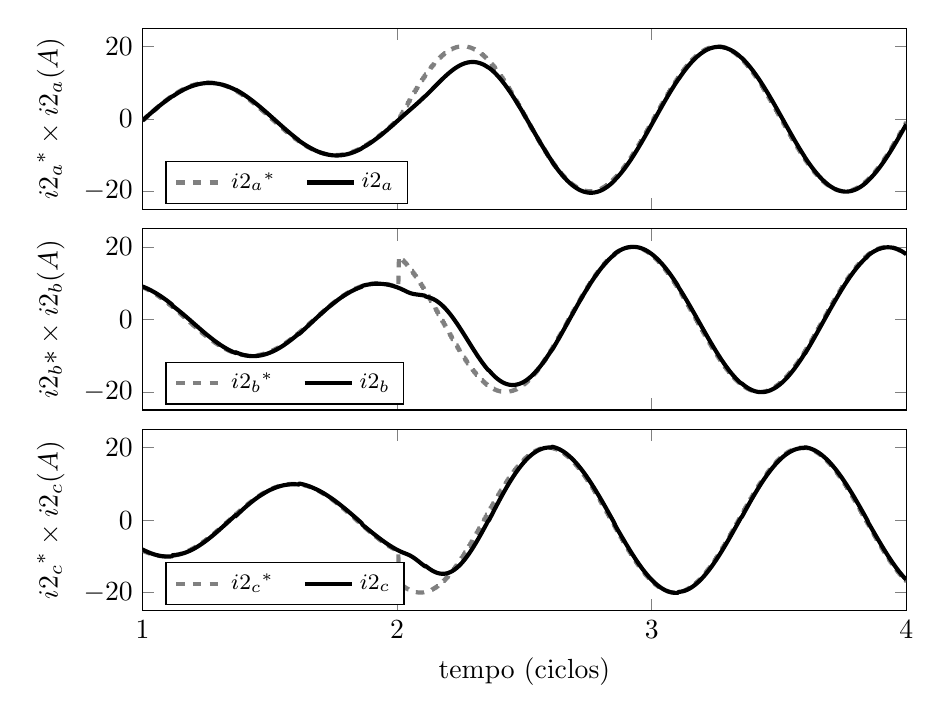
\begin{tikzpicture}

\begin{axis}[%
width=0.8\textwidth,
height=0.189701500343624\textwidth,
scale only axis,
xmin=0.0166666666666667,
xmax=0.0666666666666667,
xtick={0.0166666666666667,0.0333333333333333,0.05,0.0666666666666667},
xticklabels={\empty},
ymin=-25,
ymax=25,
ytick={-20,   0,  20},
ylabel={${\text{i2}_\text{b}}\text{* }\times\text{ i2}_\text{b}\text{ (A)}$},
name=plot2,
legend style={at={(0.03,0.03)},anchor=south west,draw=black,fill=white,legend cell align=left},
scaled x ticks = false,
legend columns=-1,
legend style={/tikz/every even column/.append style={column sep=0.3cm}},
legend style={font=\footnotesize}
]
\addplot [color=gray,dashed,line width=1.5pt]
  table[row sep=crcr]{0.0166583333333333	8.95711760239421\\
0.0167	8.81303452065\\
0.0167416666666667	8.81303452065\\
0.0167833333333333	8.66025403784447\\
0.016825	8.66025403784447\\
0.0168666666666667	8.49892692986872\\
0.0169083333333333	8.49892692986872\\
0.01695	8.32921240710107\\
0.0169916666666667	8.32921240710107\\
0.0170333333333333	8.15127795728562\\
0.017075	8.15127795728562\\
0.0171166666666667	7.96529918024204\\
0.0171583333333333	7.96529918024204\\
0.0172	7.77145961456979\\
0.0172416666666667	7.77145961456979\\
0.0172833333333333	7.56995055651764\\
0.017325	7.56995055651764\\
0.0173666666666667	7.36097087119742\\
0.0174083333333333	7.36097087119742\\
0.01745	7.1447267963281\\
0.0174916666666667	7.1447267963281\\
0.0175333333333333	6.92143173870414\\
0.017575	6.92143173870414\\
0.0176166666666667	6.69130606358865\\
0.0176583333333333	6.69130606358865\\
0.0177	6.45457687723957\\
0.0177416666666667	6.45457687723957\\
0.0177833333333333	6.21147780278317\\
0.017825	6.21147780278317\\
0.0178666666666667	5.96224874965622\\
0.0179083333333333	5.96224874965622\\
0.01795	5.70713567684438\\
0.0179916666666667	5.70713567684438\\
0.0180333333333333	5.44639035015033\\
0.018075	5.44639035015033\\
0.0181166666666667	5.18027009373136\\
0.0181583333333333	5.18027009373136\\
0.0182	4.90903753615147\\
0.0182416666666667	4.90903753615147\\
0.0182833333333333	4.63296035119867\\
0.018325	4.63296035119867\\
0.0183666666666667	4.35231099372333\\
0.0184083333333333	4.35231099372333\\
0.01845	4.06736643075805\\
0.0184916666666667	4.06736643075805\\
0.0185333333333333	3.77840786818472\\
0.018575	3.77840786818472\\
0.0186166666666667	3.4857204732182\\
0.0186583333333333	3.4857204732182\\
0.0187	3.18959309298074\\
0.0187416666666667	3.18959309298074\\
0.0187833333333333	2.89031796944476\\
0.018825	2.89031796944476\\
0.0188666666666667	2.58819045102524\\
0.0189083333333333	2.58819045102524\\
0.01895	2.28350870110659\\
0.0189916666666667	2.28350870110659\\
0.0190333333333333	1.97657340379129\\
0.019075	1.97657340379129\\
0.0191166666666667	1.66768746716105\\
0.0191583333333333	1.66768746716105\\
0.0192	1.35715572434307\\
0.0192416666666667	1.35715572434307\\
0.0192833333333333	1.04528463267656\\
0.019325	1.04528463267656\\
0.0193666666666667	0.732381971276336\\
0.0194083333333333	0.732381971276336\\
0.01945	0.418756537292012\\
0.0194916666666667	0.418756537292012\\
0.0195333333333333	0.104717841162471\\
0.019575	0.104717841162471\\
0.0196166666666667	-0.20942419883356\\
0.0196583333333333	-0.20942419883356\\
0.0197	-0.523359562429432\\
0.0197416666666667	-0.523359562429432\\
0.0197833333333333	-0.836778433323152\\
0.019825	-0.836778433323152\\
0.0198666666666667	-1.14937150492867\\
0.0199083333333333	-1.14937150492867\\
0.01995	-1.46083028562412\\
0.0199916666666667	-1.46083028562412\\
0.0200333333333333	-1.77084740319584\\
0.020075	-1.77084740319584\\
0.0201166666666667	-2.0791169081776\\
0.0201583333333333	-2.0791169081776\\
0.0202	-2.38533457578582\\
0.0202416666666667	-2.38533457578582\\
0.0202833333333333	-2.68919820615267\\
0.020325	-2.68919820615267\\
0.0203666666666667	-2.99040792256089\\
0.0204083333333333	-2.99040792256089\\
0.02045	-3.28866646738586\\
0.0204916666666667	-3.28866646738586\\
0.0205333333333333	-3.58367949545303\\
0.020575	-3.58367949545303\\
0.0206166666666667	-3.87515586452106\\
0.0206583333333333	-3.87515586452106\\
0.0207	-4.16280792260405\\
0.0207416666666667	-4.16280792260405\\
0.0207833333333333	-4.44635179184931\\
0.020825	-4.44635179184931\\
0.0208666666666667	-4.72550764869058\\
0.0209083333333333	-4.72550764869058\\
0.02095	-5.00000000000005\\
0.0209916666666667	-5.00000000000005\\
0.0210333333333333	-5.26955795496682\\
0.021075	-5.26955795496682\\
0.0211166666666667	-5.53391549243349\\
0.0211583333333333	-5.53391549243349\\
0.0212	-5.79281172342684\\
0.0212416666666667	-5.79281172342684\\
0.0212833333333333	-6.0459911486238\\
0.021325	-6.0459911486238\\
0.0213666666666667	-6.29320391049844\\
0.0214083333333333	-6.29320391049844\\
0.02145	-6.53420603990112\\
0.0214916666666667	-6.53420603990112\\
0.0215333333333333	-6.76875969682667\\
0.021575	-6.76875969682667\\
0.0216166666666667	-6.99663340513372\\
0.0216583333333333	-6.99663340513372\\
0.0217	-7.2176022809837\\
0.0217416666666667	-7.2176022809837\\
0.0217833333333333	-7.43144825477402\\
0.021825	-7.43144825477402\\
0.0218666666666667	-7.6379602863465\\
0.0219083333333333	-7.6379602863465\\
0.02195	-7.83693457325848\\
0.0219916666666667	-7.83693457325848\\
0.0220333333333333	-8.02817475191123\\
0.022075	-8.02817475191123\\
0.0221166666666667	-8.21149209133713\\
0.0221583333333333	-8.21149209133713\\
0.0222	-8.38670567945433\\
0.0222416666666667	-8.38670567945433\\
0.0222833333333333	-8.55364260160516\\
0.022325	-8.55364260160516\\
0.0223666666666667	-8.71213811120199\\
0.0224083333333333	-8.71213811120199\\
0.02245	-8.86203579231225\\
0.0224916666666667	-8.86203579231225\\
0.0225333333333333	-9.00318771402204\\
0.022575	-9.00318771402204\\
0.0226166666666667	-9.13545457642611\\
0.0226583333333333	-9.13545457642611\\
0.0227	-9.25870584810006\\
0.0227416666666667	-9.25870584810006\\
0.0227833333333333	-9.37281989491902\\
0.022825	-9.37281989491902\\
0.0228666666666667	-9.47768410009597\\
0.0229083333333333	-9.47768410009597\\
0.02295	-9.57319497532079\\
0.0229916666666667	-9.57319497532079\\
0.0230333333333333	-9.6592582628908\\
0.023075	-9.6592582628908\\
0.0231166666666667	-9.73578902873172\\
0.0231583333333333	-9.73578902873172\\
0.0232	-9.80271174621734\\
0.0232416666666667	-9.80271174621734\\
0.0232833333333333	-9.85996037070517\\
0.023325	-9.85996037070517\\
0.0233666666666667	-9.90747840471456\\
0.0234083333333333	-9.90747840471456\\
0.02345	-9.94521895368285\\
0.0234916666666667	-9.94521895368285\\
0.0235333333333333	-9.97314477224471\\
0.023575	-9.97314477224471\\
0.0236166666666667	-9.99122830098871\\
0.0236583333333333	-9.99122830098871\\
0.0237	-9.99945169365525\\
0.0237416666666667	-9.99945169365525\\
0.0237833333333333	-9.99780683474858\\
0.023825	-9.99780683474858\\
0.0238666666666667	-9.98629534754587\\
0.0239083333333333	-9.98629534754587\\
0.02395	-9.96492859249517\\
0.0239916666666667	-9.96492859249517\\
0.0240333333333333	-9.93372765600409\\
0.024075	-9.93372765600409\\
0.0241166666666667	-9.89272332963001\\
0.0241583333333333	-9.89272332963001\\
0.0242	-9.84195607969255\\
0.0242416666666667	-9.84195607969255\\
0.0242833333333333	-9.78147600733818\\
0.024325	-9.78147600733818\\
0.0243666666666667	-9.71134279909649\\
0.0244083333333333	-9.71134279909649\\
0.02445	-9.63162566797671\\
0.0244916666666667	-9.63162566797671\\
0.0245333333333333	-9.5424032851629\\
0.024575	-9.5424032851629\\
0.0246166666666667	-9.44376370237494\\
0.0246583333333333	-9.44376370237494\\
0.0247	-9.33580426497215\\
0.0247416666666667	-9.33580426497215\\
0.0247833333333333	-9.21863151588513\\
0.024825	-9.21863151588513\\
0.0248666666666667	-9.09236109047081\\
0.0249083333333333	-9.09236109047081\\
0.02495	-8.95711760239425\\
0.0249916666666667	-8.95711760239425\\
0.0250333333333333	-8.81303452065005\\
0.025075	-8.81303452065005\\
0.0251166666666667	-8.66025403784451\\
0.0251583333333333	-8.66025403784451\\
0.0252	-8.49892692986876\\
0.0252416666666667	-8.49892692986876\\
0.0252833333333333	-8.32921240710111\\
0.025325	-8.32921240710111\\
0.0253666666666667	-8.15127795728566\\
0.0254083333333333	-8.15127795728566\\
0.02545	-7.96529918024207\\
0.0254916666666667	-7.96529918024207\\
0.0255333333333333	-7.77145961456982\\
0.025575	-7.77145961456982\\
0.0256166666666667	-7.56995055651767\\
0.0256583333333333	-7.56995055651767\\
0.0257	-7.36097087119745\\
0.0257416666666667	-7.36097087119745\\
0.0257833333333333	-7.14472679632814\\
0.025825	-7.14472679632814\\
0.0258666666666667	-6.92143173870417\\
0.0259083333333333	-6.92143173870417\\
0.02595	-6.69130606358868\\
0.0259916666666667	-6.69130606358868\\
0.0260333333333333	-6.4545768772396\\
0.026075	-6.4545768772396\\
0.0261166666666667	-6.2114778027832\\
0.0261583333333333	-6.2114778027832\\
0.0262	-5.96224874965625\\
0.0262416666666667	-5.96224874965625\\
0.0262833333333333	-5.70713567684441\\
0.026325	-5.70713567684441\\
0.0263666666666667	-5.44639035015036\\
0.0264083333333333	-5.44639035015036\\
0.02645	-5.18027009373139\\
0.0264916666666667	-5.18027009373139\\
0.0265333333333333	-4.90903753615149\\
0.026575	-4.90903753615149\\
0.0266166666666667	-4.6329603511987\\
0.0266583333333333	-4.6329603511987\\
0.0267	-4.35231099372335\\
0.0267416666666667	-4.35231099372335\\
0.0267833333333333	-4.06736643075807\\
0.026825	-4.06736643075807\\
0.0268666666666667	-3.77840786818474\\
0.0269083333333333	-3.77840786818474\\
0.02695	-3.48572047321821\\
0.0269916666666667	-3.48572047321821\\
0.0270333333333333	-3.18959309298076\\
0.027075	-3.18959309298076\\
0.0271166666666667	-2.89031796944477\\
0.0271583333333333	-2.89031796944477\\
0.0272	-2.58819045102526\\
0.0272416666666667	-2.58819045102526\\
0.0272833333333333	-2.28350870110661\\
0.027325	-2.28350870110661\\
0.0273666666666667	-1.9765734037913\\
0.0274083333333333	-1.9765734037913\\
0.02745	-1.66768746716106\\
0.0274916666666667	-1.66768746716106\\
0.0275333333333333	-1.35715572434308\\
0.027575	-1.35715572434308\\
0.0276166666666667	-1.04528463267656\\
0.0276583333333333	-1.04528463267656\\
0.0277	-0.732381971276341\\
0.0277416666666667	-0.732381971276341\\
0.0277833333333333	-0.418756537292015\\
0.027825	-0.418756537292015\\
0.0278666666666667	-0.104717841162473\\
0.0279083333333333	-0.104717841162473\\
0.02795	0.209424198833559\\
0.0279916666666667	0.209424198833559\\
0.0280333333333333	0.523359562429433\\
0.028075	0.523359562429433\\
0.0281166666666667	0.836778433323154\\
0.0281583333333333	0.836778433323154\\
0.0282	1.14937150492867\\
0.0282416666666667	1.14937150492867\\
0.0282833333333333	1.46083028562412\\
0.028325	1.46083028562412\\
0.0283666666666667	1.77084740319585\\
0.0284083333333333	1.77084740319585\\
0.02845	2.07911690817761\\
0.0284916666666667	2.07911690817761\\
0.0285333333333333	2.38533457578583\\
0.028575	2.38533457578583\\
0.0286166666666667	2.68919820615268\\
0.0286583333333333	2.68919820615268\\
0.0287	2.9904079225609\\
0.0287416666666667	2.9904079225609\\
0.0287833333333333	3.28866646738587\\
0.028825	3.28866646738587\\
0.0288666666666667	3.58367949545304\\
0.0289083333333333	3.58367949545304\\
0.02895	3.87515586452107\\
0.0289916666666667	3.87515586452107\\
0.0290333333333333	4.16280792260406\\
0.029075	4.16280792260406\\
0.0291166666666667	4.44635179184933\\
0.0291583333333333	4.44635179184933\\
0.0292	4.7255076486906\\
0.0292416666666667	4.7255076486906\\
0.0292833333333333	5.00000000000006\\
0.029325	5.00000000000006\\
0.0293666666666667	5.26955795496684\\
0.0294083333333333	5.26955795496684\\
0.02945	5.53391549243351\\
0.0294916666666667	5.53391549243351\\
0.0295333333333333	5.79281172342686\\
0.029575	5.79281172342686\\
0.0296166666666667	6.04599114862383\\
0.0296583333333333	6.04599114862383\\
0.0297	6.29320391049846\\
0.0297416666666667	6.29320391049846\\
0.0297833333333333	6.53420603990114\\
0.029825	6.53420603990114\\
0.0298666666666667	6.7687596968267\\
0.0299083333333333	6.7687596968267\\
0.02995	6.99663340513375\\
0.0299916666666667	6.99663340513375\\
0.0300333333333333	7.21760228098372\\
0.030075	7.21760228098372\\
0.0301166666666667	7.43144825477405\\
0.0301583333333333	7.43144825477405\\
0.0302	7.63796028634653\\
0.0302416666666667	7.63796028634653\\
0.0302833333333333	7.83693457325851\\
0.030325	7.83693457325851\\
0.0303666666666667	8.02817475191126\\
0.0304083333333333	8.02817475191126\\
0.03045	8.21149209133716\\
0.0304916666666667	8.21149209133716\\
0.0305333333333333	8.38670567945436\\
0.030575	8.38670567945436\\
0.0306166666666667	8.55364260160519\\
0.0306583333333333	8.55364260160519\\
0.0307	8.71213811120203\\
0.0307416666666667	8.71213811120203\\
0.0307833333333333	8.86203579231228\\
0.030825	8.86203579231228\\
0.0308666666666667	9.00318771402207\\
0.0309083333333333	9.00318771402207\\
0.03095	9.13545457642615\\
0.0309916666666667	9.13545457642615\\
0.0310333333333333	9.25870584810009\\
0.031075	9.25870584810009\\
0.0311166666666667	9.37281989491906\\
0.0311583333333333	9.37281989491906\\
0.0312	9.477684100096\\
0.0312416666666667	9.477684100096\\
0.0312833333333333	9.57319497532082\\
0.031325	9.57319497532082\\
0.0313666666666667	9.65925826289084\\
0.0314083333333333	9.65925826289084\\
0.03145	9.73578902873176\\
0.0314916666666667	9.73578902873176\\
0.0315333333333333	9.80271174621738\\
0.031575	9.80271174621738\\
0.0316166666666667	9.85996037070521\\
0.0316583333333333	9.85996037070521\\
0.0317	9.9074784047146\\
0.0317416666666667	9.9074784047146\\
0.0317833333333333	9.94521895368289\\
0.031825	9.94521895368289\\
0.0318666666666667	9.97314477224474\\
0.0319083333333333	9.97314477224474\\
0.03195	9.99122830098875\\
0.0319916666666667	9.99122830098875\\
0.0320333333333333	9.99945169365528\\
0.032075	9.99945169365528\\
0.0321166666666667	9.99780683474862\\
0.0321583333333333	9.99780683474862\\
0.0322	9.98629534754591\\
0.0322416666666667	9.98629534754591\\
0.0322833333333333	9.96492859249521\\
0.032325	9.96492859249521\\
0.0323666666666667	9.93372765600413\\
0.0324083333333333	9.93372765600413\\
0.03245	9.89272332963005\\
0.0324916666666667	9.89272332963005\\
0.0325333333333333	9.84195607969259\\
0.032575	9.84195607969259\\
0.0326166666666667	9.78147600733822\\
0.0326583333333333	9.78147600733822\\
0.0327	9.71134279909653\\
0.0327416666666667	9.71134279909653\\
0.0327833333333333	9.63162566797675\\
0.032825	9.63162566797675\\
0.0328666666666667	9.54240328516294\\
0.0329083333333333	9.54240328516294\\
0.03295	9.44376370237498\\
0.0329916666666667	9.44376370237498\\
0.0330333333333333	9.33580426497218\\
0.033075	9.33580426497218\\
0.0331166666666667	9.21863151588517\\
0.0331583333333333	9.21863151588517\\
0.0332	9.09236109047085\\
0.0332416666666667	9.09236109047085\\
0.0332833333333333	8.95711760239429\\
0.033325	8.95711760239429\\
0.0333666666666667	8.81303452065008\\
0.0334083333333333	8.81303452065008\\
0.03345	17.3205080756891\\
0.0334916666666667	17.3205080756891\\
0.0335333333333333	16.9978538597376\\
0.033575	16.9978538597376\\
0.0336166666666667	16.6584248142023\\
0.0336583333333333	16.6584248142023\\
0.0337	16.3025559145714\\
0.0337416666666667	16.3025559145714\\
0.0337833333333333	15.9305983604842\\
0.033825	15.9305983604842\\
0.0338666666666667	15.5429192291397\\
0.0339083333333333	15.5429192291397\\
0.03395	15.1399011130354\\
0.0339916666666667	15.1399011130354\\
0.0340333333333333	14.721941742395\\
0.034075	14.721941742395\\
0.0341166666666667	14.2894535926563\\
0.0341583333333333	14.2894535926563\\
0.0342	13.8428634774084\\
0.0342416666666667	13.8428634774084\\
0.0342833333333333	13.3826121271774\\
0.034325	13.3826121271774\\
0.0343666666666667	12.9091537544793\\
0.0344083333333333	12.9091537544793\\
0.03445	12.4229556055665\\
0.0344916666666667	12.4229556055665\\
0.0345333333333333	11.9244974993126\\
0.034575	11.9244974993126\\
0.0346166666666667	11.4142713536889\\
0.0346583333333333	11.4142713536889\\
0.0347	10.8927807003008\\
0.0347416666666667	10.8927807003008\\
0.0347833333333333	10.3605401874628\\
0.034825	10.3605401874628\\
0.0348666666666667	9.81807507230302\\
0.0349083333333333	9.81807507230302\\
0.03495	9.26592070239743\\
0.0349916666666667	9.26592070239743\\
0.0350333333333333	8.70462198744674\\
0.035075	8.70462198744674\\
0.0351166666666667	8.13473286151618\\
0.0351583333333333	8.13473286151618\\
0.0352	7.55681573636951\\
0.0352416666666667	7.55681573636951\\
0.0352833333333333	6.97144094643646\\
0.035325	6.97144094643646\\
0.0353666666666667	6.37918618596155\\
0.0354083333333333	6.37918618596155\\
0.03545	5.78063593888957\\
0.0354916666666667	5.78063593888957\\
0.0355333333333333	5.17638090205054\\
0.035575	5.17638090205054\\
0.0356166666666667	4.56701740221323\\
0.0356583333333333	4.56701740221323\\
0.0357	3.95314680758263\\
0.0357416666666667	3.95314680758263\\
0.0357833333333333	3.33537493432214\\
0.035825	3.33537493432214\\
0.0358666666666667	2.71431144868617\\
0.0359083333333333	2.71431144868617\\
0.03595	2.09056926535314\\
0.0359916666666667	2.09056926535314\\
0.0360333333333333	1.4647639425527\\
0.036075	1.4647639425527\\
0.0361166666666667	0.837513074584043\\
0.0361583333333333	0.837513074584043\\
0.0362	0.209435682324955\\
0.0362416666666667	0.209435682324955\\
0.0362833333333333	-0.418848397667113\\
0.036325	-0.418848397667113\\
0.0363666666666667	-1.04671912485886\\
0.0364083333333333	-1.04671912485886\\
0.03645	-1.67355686664631\\
0.0364916666666667	-1.67355686664631\\
0.0365333333333333	-2.29874300985734\\
0.036575	-2.29874300985734\\
0.0366166666666667	-2.92166057124825\\
0.0366583333333333	-2.92166057124825\\
0.0367	-3.5416948063917\\
0.0367416666666667	-3.5416948063917\\
0.0367833333333333	-4.15823381635523\\
0.036825	-4.15823381635523\\
0.0368666666666667	-4.77066915157168\\
0.0369083333333333	-4.77066915157168\\
0.03695	-5.37839641230538\\
0.0369916666666667	-5.37839641230538\\
0.0370333333333333	-5.98081584512182\\
0.037075	-5.98081584512182\\
0.0371166666666667	-6.57733293477176\\
0.0371583333333333	-6.57733293477176\\
0.0372	-7.16735899090611\\
0.0372416666666667	-7.16735899090611\\
0.0372833333333333	-7.75031172904218\\
0.037325	-7.75031172904218\\
0.0373666666666667	-8.32561584520815\\
0.0374083333333333	-8.32561584520815\\
0.03745	-8.89270358369869\\
0.0374916666666667	-8.89270358369869\\
0.0375333333333333	-9.45101529738123\\
0.037575	-9.45101529738123\\
0.0376166666666667	-10.0000000000002\\
0.0376583333333333	-10.0000000000002\\
0.0377	-10.5391159099337\\
0.0377416666666667	-10.5391159099337\\
0.0377833333333333	-11.0678309848671\\
0.037825	-11.0678309848671\\
0.0378666666666667	-11.5856234468538\\
0.0379083333333333	-11.5856234468538\\
0.03795	-12.0919822972477\\
0.0379916666666667	-12.0919822972477\\
0.0380333333333333	-12.586407820997\\
0.038075	-12.586407820997\\
0.0381166666666667	-13.0684120798023\\
0.0381583333333333	-13.0684120798023\\
0.0382	-13.5375193936535\\
0.0382416666666667	-13.5375193936535\\
0.0382833333333333	-13.9932668102676\\
0.038325	-13.9932668102676\\
0.0383666666666667	-14.4352045619675\\
0.0384083333333333	-14.4352045619675\\
0.03845	-14.8628965095482\\
0.0384916666666667	-14.8628965095482\\
0.0385333333333333	-15.2759205726931\\
0.038575	-15.2759205726931\\
0.0386166666666667	-15.6738691465171\\
0.0386583333333333	-15.6738691465171\\
0.0387	-16.0563495038226\\
0.0387416666666667	-16.0563495038226\\
0.0387833333333333	-16.4229841826744\\
0.038825	-16.4229841826744\\
0.0388666666666667	-16.7734113589088\\
0.0389083333333333	-16.7734113589088\\
0.03895	-17.1072852032105\\
0.0389916666666667	-17.1072852032105\\
0.0390333333333333	-17.4242762224041\\
0.039075	-17.4242762224041\\
0.0391166666666667	-17.7240715846246\\
0.0391583333333333	-17.7240715846246\\
0.0392	-18.0063754280442\\
0.0392416666666667	-18.0063754280442\\
0.0392833333333333	-18.2709091528524\\
0.039325	-18.2709091528524\\
0.0393666666666667	-18.5174116962003\\
0.0394083333333333	-18.5174116962003\\
0.03945	-18.7456397898382\\
0.0394916666666667	-18.7456397898382\\
0.0395333333333333	-18.9553682001921\\
0.039575	-18.9553682001921\\
0.0396166666666667	-19.1463899506417\\
0.0396583333333333	-19.1463899506417\\
0.0397	-19.3185165257817\\
0.0397416666666667	-19.3185165257817\\
0.0397833333333333	-19.4715780574636\\
0.039825	-19.4715780574636\\
0.0398666666666667	-19.6054234924348\\
0.0399083333333333	-19.6054234924348\\
0.03995	-19.7199207414105\\
0.0399916666666667	-19.7199207414105\\
0.0400333333333333	-19.8149568094293\\
0.040075	-19.8149568094293\\
0.0401166666666667	-19.8904379073659\\
0.0401583333333333	-19.8904379073659\\
0.0402	-19.9462895444896\\
0.0402416666666667	-19.9462895444896\\
0.0402833333333333	-19.9824566019776\\
0.040325	-19.9824566019776\\
0.0403666666666667	-19.9989033873107\\
0.0404083333333333	-19.9989033873107\\
0.04045	-19.9956136694973\\
0.0404916666666667	-19.9956136694973\\
0.0405333333333333	-19.9725906950919\\
0.040575	-19.9725906950919\\
0.0406166666666667	-19.9298571849905\\
0.0406583333333333	-19.9298571849905\\
0.0407	-19.8674553120083\\
0.0407416666666667	-19.8674553120083\\
0.0407833333333333	-19.7854466592602\\
0.040825	-19.7854466592602\\
0.0408666666666667	-19.6839121593853\\
0.0409083333333333	-19.6839121593853\\
0.04095	-19.5629520146765\\
0.0409916666666667	-19.5629520146765\\
0.0410333333333333	-19.4226855981931\\
0.041075	-19.4226855981931\\
0.0411166666666667	-19.2632513359536\\
0.0411583333333333	-19.2632513359536\\
0.0412	-19.084806570326\\
0.0412416666666667	-19.084806570326\\
0.0412833333333333	-18.88752740475\\
0.041325	-18.88752740475\\
0.0413666666666667	-18.6716085299444\\
0.0414083333333333	-18.6716085299444\\
0.04145	-18.4372630317704\\
0.0414916666666667	-18.4372630317704\\
0.0415333333333333	-18.1847221809418\\
0.041575	-18.1847221809418\\
0.0416166666666667	-17.9142352047887\\
0.0416583333333333	-17.9142352047887\\
0.0417	-17.6260690413002\\
0.0417416666666667	-17.6260690413002\\
0.0417833333333333	-17.3205080756892\\
0.041825	-17.3205080756892\\
0.0418666666666667	-16.9978538597377\\
0.0419083333333333	-16.9978538597377\\
0.04195	-16.6584248142024\\
0.0419916666666667	-16.6584248142024\\
0.0420333333333333	-16.3025559145715\\
0.042075	-16.3025559145715\\
0.0421166666666667	-15.9305983604843\\
0.0421583333333333	-15.9305983604843\\
0.0422	-15.5429192291398\\
0.0422416666666667	-15.5429192291398\\
0.0422833333333333	-15.1399011130355\\
0.042325	-15.1399011130355\\
0.0423666666666667	-14.721941742395\\
0.0424083333333333	-14.721941742395\\
0.04245	-14.2894535926564\\
0.0424916666666667	-14.2894535926564\\
0.0425333333333333	-13.8428634774085\\
0.042575	-13.8428634774085\\
0.0426166666666667	-13.3826121271775\\
0.0426583333333333	-13.3826121271775\\
0.0427	-12.9091537544793\\
0.0427416666666667	-12.9091537544793\\
0.0427833333333333	-12.4229556055665\\
0.042825	-12.4229556055665\\
0.0428666666666667	-11.9244974993126\\
0.0429083333333333	-11.9244974993126\\
0.04295	-11.4142713536889\\
0.0429916666666667	-11.4142713536889\\
0.0430333333333333	-10.8927807003008\\
0.043075	-10.8927807003008\\
0.0431166666666667	-10.3605401874629\\
0.0431583333333333	-10.3605401874629\\
0.0432	-9.81807507230306\\
0.0432416666666667	-9.81807507230306\\
0.0432833333333333	-9.26592070239747\\
0.043325	-9.26592070239747\\
0.0433666666666667	-8.70462198744678\\
0.0434083333333333	-8.70462198744678\\
0.04345	-8.13473286151622\\
0.0434916666666667	-8.13473286151622\\
0.0435333333333333	-7.55681573636955\\
0.043575	-7.55681573636955\\
0.0436166666666667	-6.97144094643649\\
0.0436583333333333	-6.97144094643649\\
0.0437	-6.37918618596158\\
0.0437416666666667	-6.37918618596158\\
0.0437833333333333	-5.7806359388896\\
0.043825	-5.7806359388896\\
0.0438666666666667	-5.17638090205057\\
0.0439083333333333	-5.17638090205057\\
0.04395	-4.56701740221326\\
0.0439916666666667	-4.56701740221326\\
0.0440333333333333	-3.95314680758265\\
0.044075	-3.95314680758265\\
0.0441166666666667	-3.33537493432216\\
0.0441583333333333	-3.33537493432216\\
0.0442	-2.71431144868619\\
0.0442416666666667	-2.71431144868619\\
0.0442833333333333	-2.09056926535316\\
0.044325	-2.09056926535316\\
0.0443666666666667	-1.46476394255271\\
0.0444083333333333	-1.46476394255271\\
0.04445	-0.83751307458405\\
0.0444916666666667	-0.83751307458405\\
0.0445333333333333	-0.209435682324959\\
0.044575	-0.209435682324959\\
0.0446166666666667	0.418848397667111\\
0.0446583333333333	0.418848397667111\\
0.0447	1.04671912485886\\
0.0447416666666667	1.04671912485886\\
0.0447833333333333	1.67355686664631\\
0.044825	1.67355686664631\\
0.0448666666666667	2.29874300985735\\
0.0449083333333333	2.29874300985735\\
0.04495	2.92166057124826\\
0.0449916666666667	2.92166057124826\\
0.0450333333333333	3.54169480639171\\
0.045075	3.54169480639171\\
0.0451166666666667	4.15823381635525\\
0.0451583333333333	4.15823381635525\\
0.0452	4.77066915157169\\
0.0452416666666667	4.77066915157169\\
0.0452833333333333	5.37839641230541\\
0.045325	5.37839641230541\\
0.0453666666666667	5.98081584512184\\
0.0454083333333333	5.98081584512184\\
0.04545	6.57733293477179\\
0.0454916666666667	6.57733293477179\\
0.0455333333333333	7.16735899090614\\
0.045575	7.16735899090614\\
0.0456166666666667	7.75031172904221\\
0.0456583333333333	7.75031172904221\\
0.0457	8.32561584520819\\
0.0457416666666667	8.32561584520819\\
0.0457833333333333	8.89270358369873\\
0.045825	8.89270358369873\\
0.0458666666666667	9.45101529738127\\
0.0459083333333333	9.45101529738127\\
0.04595	10.0000000000002\\
0.0459916666666667	10.0000000000002\\
0.0460333333333333	10.5391159099338\\
0.046075	10.5391159099338\\
0.0461166666666667	11.0678309848671\\
0.0461583333333333	11.0678309848671\\
0.0462	11.5856234468538\\
0.0462416666666667	11.5856234468538\\
0.0462833333333333	12.0919822972478\\
0.046325	12.0919822972478\\
0.0463666666666667	12.586407820997\\
0.0464083333333333	12.586407820997\\
0.04645	13.0684120798024\\
0.0464916666666667	13.0684120798024\\
0.0465333333333333	13.5375193936535\\
0.046575	13.5375193936535\\
0.0466166666666667	13.9932668102676\\
0.0466583333333333	13.9932668102676\\
0.0467	14.4352045619676\\
0.0467416666666667	14.4352045619676\\
0.0467833333333333	14.8628965095482\\
0.046825	14.8628965095482\\
0.0468666666666667	15.2759205726932\\
0.0469083333333333	15.2759205726932\\
0.04695	15.6738691465172\\
0.0469916666666667	15.6738691465172\\
0.0470333333333333	16.0563495038227\\
0.047075	16.0563495038227\\
0.0471166666666667	16.4229841826745\\
0.0471583333333333	16.4229841826745\\
0.0472	16.7734113589089\\
0.0472416666666667	16.7734113589089\\
0.0472833333333333	17.1072852032105\\
0.047325	17.1072852032105\\
0.0473666666666667	17.4242762224042\\
0.0474083333333333	17.4242762224042\\
0.04745	17.7240715846247\\
0.0474916666666667	17.7240715846247\\
0.0475333333333333	18.0063754280443\\
0.047575	18.0063754280443\\
0.0476166666666667	18.2709091528525\\
0.0476583333333333	18.2709091528525\\
0.0477	18.5174116962003\\
0.0477416666666667	18.5174116962003\\
0.0477833333333333	18.7456397898383\\
0.047825	18.7456397898383\\
0.0478666666666667	18.9553682001922\\
0.0479083333333333	18.9553682001922\\
0.04795	19.1463899506418\\
0.0479916666666667	19.1463899506418\\
0.0480333333333333	19.3185165257818\\
0.048075	19.3185165257818\\
0.0481166666666667	19.4715780574637\\
0.0481583333333333	19.4715780574637\\
0.0482	19.6054234924349\\
0.0482416666666667	19.6054234924349\\
0.0482833333333333	19.7199207414106\\
0.048325	19.7199207414106\\
0.0483666666666667	19.8149568094294\\
0.0484083333333333	19.8149568094294\\
0.04845	19.890437907366\\
0.0484916666666667	19.890437907366\\
0.0485333333333333	19.9462895444897\\
0.048575	19.9462895444897\\
0.0486166666666667	19.9824566019777\\
0.0486583333333333	19.9824566019777\\
0.0487	19.9989033873107\\
0.0487416666666667	19.9989033873107\\
0.0487833333333333	19.9956136694974\\
0.048825	19.9956136694974\\
0.0488666666666667	19.972590695092\\
0.0489083333333333	19.972590695092\\
0.04895	19.9298571849906\\
0.0489916666666667	19.9298571849906\\
0.0490333333333333	19.8674553120084\\
0.049075	19.8674553120084\\
0.0491166666666667	19.7854466592603\\
0.0491583333333333	19.7854466592603\\
0.0492	19.6839121593854\\
0.0492416666666667	19.6839121593854\\
0.0492833333333333	19.5629520146766\\
0.049325	19.5629520146766\\
0.0493666666666667	19.4226855981932\\
0.0494083333333333	19.4226855981932\\
0.04945	19.2632513359537\\
0.0494916666666667	19.2632513359537\\
0.0495333333333333	19.084806570326\\
0.049575	19.084806570326\\
0.0496166666666667	18.8875274047501\\
0.0496583333333333	18.8875274047501\\
0.0497	18.6716085299445\\
0.0497416666666667	18.6716085299445\\
0.0497833333333333	18.4372630317705\\
0.049825	18.4372630317705\\
0.0498666666666667	18.1847221809419\\
0.0499083333333333	18.1847221809419\\
0.04995	17.9142352047887\\
0.0499916666666667	17.9142352047887\\
0.0500333333333333	17.6260690413003\\
0.050075	17.6260690413003\\
0.0501166666666667	17.3205080756892\\
0.0501583333333333	17.3205080756892\\
0.0502	16.9978538597377\\
0.0502416666666667	16.9978538597377\\
0.0502833333333333	16.6584248142025\\
0.050325	16.6584248142025\\
0.0503666666666667	16.3025559145715\\
0.0504083333333333	16.3025559145715\\
0.05045	15.9305983604844\\
0.0504916666666667	15.9305983604844\\
0.0505333333333333	15.5429192291399\\
0.050575	15.5429192291399\\
0.0506166666666667	15.1399011130356\\
0.0506583333333333	15.1399011130356\\
0.0507	14.7219417423951\\
0.0507416666666667	14.7219417423951\\
0.0507833333333333	14.2894535926565\\
0.050825	14.2894535926565\\
0.0508666666666667	13.8428634774085\\
0.0509083333333333	13.8428634774085\\
0.05095	13.3826121271776\\
0.0509916666666667	13.3826121271776\\
0.0510333333333333	12.9091537544794\\
0.051075	12.9091537544794\\
0.0511166666666667	12.4229556055666\\
0.0511583333333333	12.4229556055666\\
0.0512	11.9244974993127\\
0.0512416666666667	11.9244974993127\\
0.0512833333333333	11.414271353689\\
0.051325	11.414271353689\\
0.0513666666666667	10.8927807003009\\
0.0514083333333333	10.8927807003009\\
0.05145	10.3605401874629\\
0.0514916666666667	10.3605401874629\\
0.0515333333333333	9.81807507230311\\
0.051575	9.81807507230311\\
0.0516166666666667	9.26592070239752\\
0.0516583333333333	9.26592070239752\\
0.0517	8.70462198744682\\
0.0517416666666667	8.70462198744682\\
0.0517833333333333	8.13473286151626\\
0.051825	8.13473286151626\\
0.0518666666666667	7.55681573636959\\
0.0519083333333333	7.55681573636959\\
0.05195	6.97144094643653\\
0.0519916666666667	6.97144094643653\\
0.0520333333333333	6.37918618596161\\
0.052075	6.37918618596161\\
0.0521166666666667	5.78063593888963\\
0.0521583333333333	5.78063593888963\\
0.0522	5.1763809020506\\
0.0522416666666667	5.1763809020506\\
0.0522833333333333	4.56701740221328\\
0.052325	4.56701740221328\\
0.0523666666666667	3.95314680758267\\
0.0524083333333333	3.95314680758267\\
0.05245	3.33537493432218\\
0.0524916666666667	3.33537493432218\\
0.0525333333333333	2.71431144868621\\
0.052575	2.71431144868621\\
0.0526166666666667	2.09056926535317\\
0.0526583333333333	2.09056926535317\\
0.0527	1.46476394255272\\
0.0527416666666667	1.46476394255272\\
0.0527833333333333	0.837513074584059\\
0.052825	0.837513074584059\\
0.0528666666666667	0.209435682324965\\
0.0529083333333333	0.209435682324965\\
0.05295	-0.418848397667108\\
0.0529916666666667	-0.418848397667108\\
0.0530333333333333	-1.04671912485886\\
0.053075	-1.04671912485886\\
0.0531166666666667	-1.67355686664631\\
0.0531583333333333	-1.67355686664631\\
0.0532	-2.29874300985735\\
0.0532416666666667	-2.29874300985735\\
0.0532833333333333	-2.92166057124827\\
0.053325	-2.92166057124827\\
0.0533666666666667	-3.54169480639172\\
0.0534083333333333	-3.54169480639172\\
0.05345	-4.15823381635526\\
0.0534916666666667	-4.15823381635526\\
0.0535333333333333	-4.77066915157171\\
0.053575	-4.77066915157171\\
0.0536166666666667	-5.37839641230542\\
0.0536583333333333	-5.37839641230542\\
0.0537	-5.98081584512186\\
0.0537416666666667	-5.98081584512186\\
0.0537833333333333	-6.57733293477181\\
0.053825	-6.57733293477181\\
0.0538666666666667	-7.16735899090617\\
0.0539083333333333	-7.16735899090617\\
0.05395	-7.75031172904224\\
0.0539916666666667	-7.75031172904224\\
0.0540333333333333	-8.32561584520822\\
0.054075	-8.32561584520822\\
0.0541166666666667	-8.89270358369876\\
0.0541583333333333	-8.89270358369876\\
0.0542	-9.45101529738131\\
0.0542416666666667	-9.45101529738131\\
0.0542833333333333	-10.0000000000002\\
0.054325	-10.0000000000002\\
0.0543666666666667	-10.5391159099338\\
0.0544083333333333	-10.5391159099338\\
0.05445	-11.0678309848672\\
0.0544916666666667	-11.0678309848672\\
0.0545333333333333	-11.5856234468539\\
0.054575	-11.5856234468539\\
0.0546166666666667	-12.0919822972478\\
0.0546583333333333	-12.0919822972478\\
0.0547	-12.5864078209971\\
0.0547416666666667	-12.5864078209971\\
0.0547833333333333	-13.0684120798024\\
0.054825	-13.0684120798024\\
0.0548666666666667	-13.5375193936536\\
0.0549083333333333	-13.5375193936536\\
0.05495	-13.9932668102677\\
0.0549916666666667	-13.9932668102677\\
0.0550333333333333	-14.4352045619676\\
0.055075	-14.4352045619676\\
0.0551166666666667	-14.8628965095483\\
0.0551583333333333	-14.8628965095483\\
0.0552	-15.2759205726933\\
0.0552416666666667	-15.2759205726933\\
0.0552833333333333	-15.6738691465172\\
0.055325	-15.6738691465172\\
0.0553666666666667	-16.0563495038227\\
0.0554083333333333	-16.0563495038227\\
0.05545	-16.4229841826745\\
0.0554916666666667	-16.4229841826745\\
0.0555333333333333	-16.7734113589089\\
0.055575	-16.7734113589089\\
0.0556166666666667	-17.1072852032106\\
0.0556583333333333	-17.1072852032106\\
0.0557	-17.4242762224043\\
0.0557416666666667	-17.4242762224043\\
0.0557833333333333	-17.7240715846248\\
0.055825	-17.7240715846248\\
0.0558666666666667	-18.0063754280444\\
0.0559083333333333	-18.0063754280444\\
0.05595	-18.2709091528525\\
0.0559916666666667	-18.2709091528525\\
0.0560333333333333	-18.5174116962004\\
0.056075	-18.5174116962004\\
0.0561166666666667	-18.7456397898384\\
0.0561583333333333	-18.7456397898384\\
0.0562	-18.9553682001923\\
0.0562416666666667	-18.9553682001923\\
0.0562833333333333	-19.1463899506419\\
0.056325	-19.1463899506419\\
0.0563666666666667	-19.3185165257819\\
0.0564083333333333	-19.3185165257819\\
0.05645	-19.4715780574638\\
0.0564916666666667	-19.4715780574638\\
0.0565333333333333	-19.605423492435\\
0.056575	-19.605423492435\\
0.0566166666666667	-19.7199207414107\\
0.0566583333333333	-19.7199207414107\\
0.0567	-19.8149568094295\\
0.0567416666666667	-19.8149568094295\\
0.0567833333333333	-19.890437907366\\
0.056825	-19.890437907366\\
0.0568666666666667	-19.9462895444897\\
0.0569083333333333	-19.9462895444897\\
0.05695	-19.9824566019778\\
0.0569916666666667	-19.9824566019778\\
0.0570333333333333	-19.9989033873108\\
0.057075	-19.9989033873108\\
0.0571166666666667	-19.9956136694975\\
0.0571583333333333	-19.9956136694975\\
0.0572	-19.9725906950921\\
0.0572416666666667	-19.9725906950921\\
0.0572833333333333	-19.9298571849907\\
0.057325	-19.9298571849907\\
0.0573666666666667	-19.8674553120085\\
0.0574083333333333	-19.8674553120085\\
0.05745	-19.7854466592604\\
0.0574916666666667	-19.7854466592604\\
0.0575333333333333	-19.6839121593854\\
0.057575	-19.6839121593854\\
0.0576166666666667	-19.5629520146767\\
0.0576583333333333	-19.5629520146767\\
0.0577	-19.4226855981933\\
0.0577416666666667	-19.4226855981933\\
0.0577833333333333	-19.2632513359538\\
0.057825	-19.2632513359538\\
0.0578666666666667	-19.0848065703261\\
0.0579083333333333	-19.0848065703261\\
0.05795	-18.8875274047502\\
0.0579916666666667	-18.8875274047502\\
0.0580333333333333	-18.6716085299446\\
0.058075	-18.6716085299446\\
0.0581166666666667	-18.4372630317706\\
0.0581583333333333	-18.4372630317706\\
0.0582	-18.1847221809419\\
0.0582416666666667	-18.1847221809419\\
0.0582833333333333	-17.9142352047888\\
0.058325	-17.9142352047888\\
0.0583666666666667	-17.6260690413004\\
0.0584083333333333	-17.6260690413004\\
0.05845	-17.3205080756893\\
0.0584916666666667	-17.3205080756893\\
0.0585333333333333	-16.9978538597378\\
0.058575	-16.9978538597378\\
0.0586166666666667	-16.6584248142025\\
0.0586583333333333	-16.6584248142025\\
0.0587	-16.3025559145716\\
0.0587416666666667	-16.3025559145716\\
0.0587833333333333	-15.9305983604844\\
0.058825	-15.9305983604844\\
0.0588666666666667	-15.5429192291399\\
0.0589083333333333	-15.5429192291399\\
0.05895	-15.1399011130356\\
0.0589916666666667	-15.1399011130356\\
0.0590333333333333	-14.7219417423952\\
0.059075	-14.7219417423952\\
0.0591166666666667	-14.2894535926565\\
0.0591583333333333	-14.2894535926565\\
0.0592	-13.8428634774086\\
0.0592416666666667	-13.8428634774086\\
0.0592833333333333	-13.3826121271776\\
0.059325	-13.3826121271776\\
0.0593666666666667	-12.9091537544794\\
0.0594083333333333	-12.9091537544794\\
0.05945	-12.4229556055666\\
0.0594916666666667	-12.4229556055666\\
0.0595333333333333	-11.9244974993127\\
0.059575	-11.9244974993127\\
0.0596166666666667	-11.414271353689\\
0.0596583333333333	-11.414271353689\\
0.0597	-10.8927807003009\\
0.0597416666666667	-10.8927807003009\\
0.0597833333333333	-10.360540187463\\
0.059825	-10.360540187463\\
0.0598666666666667	-9.81807507230316\\
0.0599083333333333	-9.81807507230316\\
0.05995	-9.26592070239757\\
0.0599916666666667	-9.26592070239757\\
0.0600333333333333	-8.70462198744687\\
0.060075	-8.70462198744687\\
0.0601166666666667	-8.1347328615163\\
0.0601583333333333	-8.1347328615163\\
0.0602	-7.55681573636962\\
0.0602416666666667	-7.55681573636962\\
0.0602833333333333	-6.97144094643657\\
0.060325	-6.97144094643657\\
0.0603666666666667	-6.37918618596165\\
0.0604083333333333	-6.37918618596165\\
0.06045	-5.78063593888966\\
0.0604916666666667	-5.78063593888966\\
0.0605333333333333	-5.17638090205062\\
0.060575	-5.17638090205062\\
0.0606166666666667	-4.56701740221331\\
0.0606583333333333	-4.56701740221331\\
0.0607	-3.95314680758269\\
0.0607416666666667	-3.95314680758269\\
0.0607833333333333	-3.3353749343222\\
0.060825	-3.3353749343222\\
0.0608666666666667	-2.71431144868622\\
0.0609083333333333	-2.71431144868622\\
0.06095	-2.09056926535319\\
0.0609916666666667	-2.09056926535319\\
0.0610333333333333	-1.46476394255273\\
0.061075	-1.46476394255273\\
0.0611166666666667	-0.837513074584069\\
0.0611583333333333	-0.837513074584069\\
0.0612	-0.209435682324971\\
0.0612416666666667	-0.209435682324971\\
0.0612833333333333	0.418848397667104\\
0.061325	0.418848397667104\\
0.0613666666666667	1.04671912485886\\
0.0614083333333333	1.04671912485886\\
0.06145	1.67355686664631\\
0.0614916666666667	1.67355686664631\\
0.0615333333333333	2.29874300985736\\
0.061575	2.29874300985736\\
0.0616166666666667	2.92166057124828\\
0.0616583333333333	2.92166057124828\\
0.0617	3.54169480639173\\
0.0617416666666667	3.54169480639173\\
0.0617833333333333	4.15823381635527\\
0.061825	4.15823381635527\\
0.0618666666666667	4.77066915157172\\
0.0619083333333333	4.77066915157172\\
0.06195	5.37839641230544\\
0.0619916666666667	5.37839641230544\\
0.0620333333333333	5.98081584512188\\
0.062075	5.98081584512188\\
0.0621166666666667	6.57733293477183\\
0.0621583333333333	6.57733293477183\\
0.0622	7.16735899090619\\
0.0622416666666667	7.16735899090619\\
0.0622833333333333	7.75031172904226\\
0.062325	7.75031172904226\\
0.0623666666666667	8.32561584520825\\
0.0624083333333333	8.32561584520825\\
0.06245	8.89270358369879\\
0.0624916666666667	8.89270358369879\\
0.0625333333333333	9.45101529738134\\
0.062575	9.45101529738134\\
0.0626166666666667	10.0000000000003\\
0.0626583333333333	10.0000000000003\\
0.0627	10.5391159099339\\
0.0627416666666667	10.5391159099339\\
0.0627833333333333	11.0678309848672\\
0.062825	11.0678309848672\\
0.0628666666666667	11.5856234468539\\
0.0629083333333333	11.5856234468539\\
0.06295	12.0919822972478\\
0.0629916666666667	12.0919822972478\\
0.0630333333333333	12.5864078209971\\
0.063075	12.5864078209971\\
0.0631166666666667	13.0684120798025\\
0.0631583333333333	13.0684120798025\\
0.0632	13.5375193936536\\
0.0632416666666667	13.5375193936536\\
0.0632833333333333	13.9932668102677\\
0.063325	13.9932668102677\\
0.0633666666666667	14.4352045619677\\
0.0634083333333333	14.4352045619677\\
0.06345	14.8628965095483\\
0.0634916666666667	14.8628965095483\\
0.0635333333333333	15.2759205726933\\
0.063575	15.2759205726933\\
0.0636166666666667	15.6738691465173\\
0.0636583333333333	15.6738691465173\\
0.0637	16.0563495038228\\
0.0637416666666667	16.0563495038228\\
0.0637833333333333	16.4229841826746\\
0.063825	16.4229841826746\\
0.0638666666666667	16.773411358909\\
0.0639083333333333	16.773411358909\\
0.06395	17.1072852032107\\
0.0639916666666667	17.1072852032107\\
0.0640333333333333	17.4242762224043\\
0.064075	17.4242762224043\\
0.0641166666666667	17.7240715846249\\
0.0641583333333333	17.7240715846249\\
0.0642	18.0063754280444\\
0.0642416666666667	18.0063754280444\\
0.0642833333333333	18.2709091528526\\
0.064325	18.2709091528526\\
0.0643666666666667	18.5174116962005\\
0.0644083333333333	18.5174116962005\\
0.06445	18.7456397898384\\
0.0644916666666667	18.7456397898384\\
0.0645333333333333	18.9553682001923\\
0.064575	18.9553682001923\\
0.0646166666666667	19.146389950642\\
0.0646583333333333	19.146389950642\\
0.0647	19.318516525782\\
0.0647416666666667	19.318516525782\\
0.0647833333333333	19.4715780574638\\
0.064825	19.4715780574638\\
0.0648666666666667	19.6054234924351\\
0.0649083333333333	19.6054234924351\\
0.06495	19.7199207414107\\
0.0649916666666667	19.7199207414107\\
0.0650333333333333	19.8149568094295\\
0.065075	19.8149568094295\\
0.0651166666666667	19.8904379073661\\
0.0651583333333333	19.8904379073661\\
0.0652	19.9462895444898\\
0.0652416666666667	19.9462895444898\\
0.0652833333333333	19.9824566019778\\
0.065325	19.9824566019778\\
0.0653666666666667	19.9989033873109\\
0.0654083333333333	19.9989033873109\\
0.06545	19.9956136694976\\
0.0654916666666667	19.9956136694976\\
0.0655333333333333	19.9725906950921\\
0.065575	19.9725906950921\\
0.0656166666666667	19.9298571849908\\
0.0656583333333333	19.9298571849908\\
0.0657	19.8674553120086\\
0.0657416666666667	19.8674553120086\\
0.0657833333333333	19.7854466592604\\
0.065825	19.7854466592604\\
0.0658666666666667	19.6839121593855\\
0.0659083333333333	19.6839121593855\\
0.06595	19.5629520146768\\
0.0659916666666667	19.5629520146768\\
0.0660333333333333	19.4226855981934\\
0.066075	19.4226855981934\\
0.0661166666666667	19.2632513359538\\
0.0661583333333333	19.2632513359538\\
0.0662	19.0848065703262\\
0.0662416666666667	19.0848065703262\\
0.0662833333333333	18.8875274047503\\
0.066325	18.8875274047503\\
0.0663666666666667	18.6716085299447\\
0.0664083333333333	18.6716085299447\\
0.06645	18.4372630317707\\
0.0664916666666667	18.4372630317707\\
0.0665333333333333	18.184722180942\\
0.066575	18.184722180942\\
0.0666166666666667	17.9142352047889\\
0.0666583333333333	17.9142352047889\\
};
\addlegendentry{${\text{i2}_\text{b}}^\text{*}$};

\addplot [color=black,solid,line width=1.5pt]
  table[row sep=crcr]{0.0166583333333333	9.10238729436972\\
0.0167	9.03402165826534\\
0.0167416666666667	8.96368598655141\\
0.0167833333333333	8.89133568061203\\
0.016825	8.81704993622876\\
0.0168666666666667	8.74079343507884\\
0.0169083333333333	8.66265295711749\\
0.01695	8.58259781627092\\
0.0169916666666667	8.50071754137033\\
0.0170333333333333	8.41698140145812\\
0.017075	8.33147777016323\\
0.0171166666666667	8.24417239647427\\
0.0171583333333333	8.15515004140646\\
0.0172	8.06437114911801\\
0.0172416666666667	7.97191608287754\\
0.0172833333333333	7.8777397886972\\
0.017325	7.7819187867049\\
0.0173666666666667	7.68440342410503\\
0.0174083333333333	7.58526770699698\\
0.01745	7.48445879295424\\
0.0174916666666667	7.38204974177135\\
0.0175333333333333	7.27798597031744\\
0.017575	7.1723588885292\\
0.0176166666666667	7.06511633678431\\
0.0176583333333333	6.95626978050029\\
0.0177	6.84580684667755\\
0.0177416666666667	6.73380549079232\\
0.0177833333333333	6.62021165288726\\
0.017825	6.50510560395105\\
0.0178666666666667	6.38843437691671\\
0.0179083333333333	6.2702810790216\\
0.01795	6.15059383602935\\
0.0179916666666667	6.02945861112754\\
0.0180333333333333	5.9068245245065\\
0.018075	5.78278034407908\\
0.0181166666666667	5.65727605146901\\
0.0181583333333333	5.53040314356191\\
0.0182	5.40211233541475\\
0.0182416666666667	5.27249778086378\\
0.0182833333333333	5.14151082265956\\
0.018325	5.00924821301577\\
0.0183666666666667	4.87566184068634\\
0.0184083333333333	4.74085100951404\\
0.01845	4.60476809055667\\
0.0184916666666667	4.46751489796481\\
0.0185333333333333	4.32904423117766\\
0.018575	4.1894603719659\\
0.0186166666666667	3.95920493855525\\
0.0186583333333333	3.68981019134787\\
0.0187	3.55459438762532\\
0.0187416666666667	3.41994135779203\\
0.0187833333333333	3.284551150892\\
0.018825	3.14840956068264\\
0.0188666666666667	3.01131770702737\\
0.0189083333333333	2.87329876433044\\
0.01895	2.73422375637314\\
0.0189916666666667	2.59416394011585\\
0.0190333333333333	2.45303513633463\\
0.019075	2.31093742969384\\
0.0191166666666667	2.16781280767052\\
0.0191583333333333	2.02377684219615\\
0.0192	1.87878453430694\\
0.0192416666666667	1.73295860389567\\
0.0192833333333333	1.58625899975514\\
0.019325	1.43881119869898\\
0.0193666666666667	1.29057586425682\\
0.0194083333333333	1.14167948532007\\
0.01945	0.992081703949671\\
0.0194916666666667	0.841909769593364\\
0.0195333333333333	0.691121953346188\\
0.019575	0.539846655564751\\
0.0196166666666667	0.388041029571302\\
0.0196583333333333	0.235780957939821\\
0.0197	0.0831137819522103\\
0.0197416666666667	-0.0698428576316909\\
0.0197833333333333	-0.223155234126428\\
0.019825	-0.376689340170496\\
0.0198666666666667	-0.530489508286105\\
0.0199083333333333	-0.684419603756233\\
0.01995	-0.838524258952192\\
0.0199916666666667	-0.992665526242936\\
0.0200333333333333	-1.14688842282822\\
0.020075	-1.30105355347543\\
0.0201166666666667	-1.45520644787935\\
0.0201583333333333	-1.60920663242736\\
0.0202	-1.7631002680197\\
0.0202416666666667	-1.91674613701216\\
0.0202833333333333	-2.07019111926222\\
0.020325	-2.22329353670832\\
0.0203666666666667	-2.37610103952102\\
0.0204083333333333	-2.52847172237396\\
0.02045	-2.68045402642318\\
0.0204916666666667	-2.83190601073707\\
0.0205333333333333	-2.98287690775002\\
0.020575	-3.13322490271858\\
0.0206166666666667	-3.28300000950168\\
0.0206583333333333	-3.43206068203698\\
0.0207	-3.58023257831695\\
0.0207416666666667	-3.7277092334411\\
0.0207833333333333	-3.8745094495467\\
0.020825	-4.02042104637285\\
0.0208666666666667	-4.16549853373004\\
0.0209083333333333	-4.30960748092213\\
0.02095	-4.45281035993282\\
0.0209916666666667	-4.59498130928033\\
0.0210333333333333	-4.73619019464951\\
0.021075	-4.87631621588383\\
0.0211166666666667	-5.01543181083388\\
0.0211583333333333	-5.15341682461041\\
0.0212	-5.29034220696768\\
0.0212416666666667	-5.426085096601\\
0.0212833333333333	-5.56071222059019\\
0.021325	-5.6940962192604\\
0.0213666666666667	-5.82629850539151\\
0.0214083333333333	-5.95718699185082\\
0.02145	-6.08681807174369\\
0.0214916666666667	-6.21505582977236\\
0.0215333333333333	-6.34195278597919\\
0.021575	-6.4673706655078\\
0.0216166666666667	-6.59135957583495\\
0.0216583333333333	-6.71378044678016\\
0.0217	-6.83468524636737\\
0.0217416666666667	-6.95399217938414\\
0.0217833333333333	-7.07162840913448\\
0.021825	-7.18751402421548\\
0.0218666666666667	-7.30170428968836\\
0.0219083333333333	-7.4140646101137\\
0.02195	-7.52464610549204\\
0.0219916666666667	-7.6333168162301\\
0.0220333333333333	-7.74012919995476\\
0.022075	-7.84495413606052\\
0.0221166666666667	-7.94784540294816\\
0.0221583333333333	-8.04867680302019\\
0.0222	-8.14750333773792\\
0.0222416666666667	-8.24420176720482\\
0.0222833333333333	-8.33882819422802\\
0.022325	-8.43126236325755\\
0.0223666666666667	-8.52156136312858\\
0.0224083333333333	-8.60960796183905\\
0.02245	-8.69546013657608\\
0.0224916666666667	-8.77900373523377\\
0.0225333333333333	-8.86029754231411\\
0.022575	-8.93923055494087\\
0.0226166666666667	-9.0158622940634\\
0.0226583333333333	-9.09008498121201\\
0.0227	-9.1619588058232\\
0.0227416666666667	-9.21081573522\\
0.0227833333333333	-9.0984668685434\\
0.022825	-9.15855337492306\\
0.0228666666666667	-9.22947523354302\\
0.0229083333333333	-9.29819015157014\\
0.02295	-9.36464137946829\\
0.0229916666666667	-9.42861378862864\\
0.0230333333333333	-9.4900453851335\\
0.023075	-9.54876390071828\\
0.0231166666666667	-9.60476742762568\\
0.0231583333333333	-9.65793002398938\\
0.0232	-9.70828718453498\\
0.0232416666666667	-9.7557417725555\\
0.0232833333333333	-9.80035019237776\\
0.023325	-9.84203175689098\\
0.0233666666666667	-9.88085243770552\\
0.0234083333333333	-9.91674024993253\\
0.02345	-9.94976400939473\\
0.0234916666666667	-9.97985634821345\\
0.0235333333333333	-10.0070856173288\\
0.023575	-10.0313874481953\\
0.0236166666666667	-10.0528285835685\\
0.0236583333333333	-10.0713474398235\\
0.0237	-10.087009152455\\
0.0237416666666667	-10.0997553242113\\
0.0237833333333333	-10.1096212768965\\
0.023825	-10.1165549780692\\
0.0238666666666667	-10.1207046835537\\
0.0239083333333333	-10.1219620846997\\
0.02395	-10.1203887350907\\
0.0239916666666667	-10.1159383416511\\
0.0240333333333333	-10.108673385745\\
0.024075	-10.0985519776893\\
0.0241166666666667	-10.0856362616203\\
0.0241583333333333	-10.0698886487835\\
0.0242	-10.0513707563433\\
0.0242416666666667	-10.0300491222447\\
0.0242833333333333	-10.0059846094998\\
0.024325	-9.97914771255928\\
0.0243666666666667	-9.94959832122408\\
0.0244083333333333	-9.91731074942411\\
0.02445	-9.88234372724823\\
0.0244916666666667	-9.84467529451614\\
0.0245333333333333	-9.80436287400011\\
0.024575	-9.76138817764229\\
0.0246166666666667	-9.71580720736102\\
0.0246583333333333	-9.66760532286042\\
0.0247	-9.61683701630429\\
0.0247416666666667	-9.56349128839865\\
0.0247833333333333	-9.50762104775379\\
0.024825	-9.44931901487656\\
0.0248666666666667	-9.38863375961779\\
0.0249083333333333	-9.32530954504734\\
0.02495	-9.25954240579891\\
0.0249916666666667	-9.19133428032041\\
0.0250333333333333	-9.12072866075138\\
0.025075	-9.0477213069644\\
0.0251166666666667	-8.97234645727584\\
0.0251583333333333	-8.8945965624705\\
0.0252	-8.81449915043002\\
0.0252416666666667	-8.73204780656025\\
0.0252833333333333	-8.64726779224821\\
0.025325	-8.56015786213606\\
0.0253666666666667	-8.47074449149494\\
0.0254083333333333	-8.37903445036129\\
0.02545	-8.28505746633374\\
0.0254916666666667	-8.18882959610245\\
0.0255333333333333	-8.09038431584565\\
0.025575	-7.98974683729511\\
0.0256166666666667	-7.8869537101997\\
0.0256583333333333	-7.78203825639882\\
0.0257	-7.67503879052939\\
0.0257416666666667	-7.56599531459094\\
0.0257833333333333	-7.4549464461354\\
0.025825	-7.34193745850652\\
0.0258666666666667	-7.22694839894464\\
0.0259083333333333	-7.11012337980954\\
0.02595	-6.99148702983552\\
0.0259916666666667	-6.871066065311\\
0.0260333333333333	-6.74889334302512\\
0.026075	-6.6250242807278\\
0.0261166666666667	-6.49948893121508\\
0.0261583333333333	-6.37234524011466\\
0.0262	-6.24362019708288\\
0.0262416666666667	-6.11337417903073\\
0.0262833333333333	-5.98163110846722\\
0.026325	-5.84845377190004\\
0.0263666666666667	-5.71386307769823\\
0.0264083333333333	-5.57792422743959\\
0.02645	-5.44065518096032\\
0.0264916666666667	-5.30212355465025\\
0.0265333333333333	-5.16234441546605\\
0.026575	-5.02138777484591\\
0.0266166666666667	-4.87926584633126\\
0.0266583333333333	-4.73605099633701\\
0.0267	-4.59175261144144\\
0.0267416666666667	-4.44644535816739\\
0.0267833333333333	-4.30013581630143\\
0.026825	-4.15290088980286\\
0.0268666666666667	-4.00645132217426\\
0.0269083333333333	-4.00941990874226\\
0.02695	-3.90500866602108\\
0.0269916666666667	-3.7463128418275\\
0.0270333333333333	-3.58617730564843\\
0.027075	-3.42515227885231\\
0.0271166666666667	-3.26336001143087\\
0.0271583333333333	-3.10098116111065\\
0.0272	-2.93808952673461\\
0.0272416666666667	-2.77482587402537\\
0.0272833333333333	-2.61122185555184\\
0.027325	-2.44739188124668\\
0.0273666666666667	-2.28334165434491\\
0.0274083333333333	-2.11917164363188\\
0.02745	-1.95487269182209\\
0.0274916666666667	-1.79053931585367\\
0.0275333333333333	-1.6261543368841\\
0.027575	-1.4618108533529\\
0.0276166666666667	-1.29748734777055\\
0.0276583333333333	-1.13327765870239\\
0.0277	-0.969157568289885\\
0.0277416666666667	-0.805222391523657\\
0.0277833333333333	-0.641445704083668\\
0.027825	-0.477924319106184\\
0.0278666666666667	-0.314629584722561\\
0.0279083333333333	-0.151666910444537\\
0.02795	0.010929802302895\\
0.0279916666666667	0.173209663659246\\
0.0280333333333333	0.33514019087048\\
0.028075	0.496611559876445\\
0.0281166666666667	0.657659711941593\\
0.0281583333333333	0.81818389481377\\
0.0282	0.978222468495446\\
0.0282416666666667	1.13767393946308\\
0.0282833333333333	1.29657892292822\\
0.028325	1.45483512926401\\
0.0283666666666667	1.61248520279227\\
0.0284083333333333	1.76942599324087\\
0.02845	1.92570195915175\\
0.0284916666666667	2.08120905361234\\
0.0285333333333333	2.23599336371434\\
0.028575	2.38994994741015\\
0.0286166666666667	2.54312636983508\\
0.0286583333333333	2.69541683114933\\
0.0287	2.84687025538406\\
0.0287416666666667	2.99738005024818\\
0.0287833333333333	3.14699640262514\\
0.028825	3.29561201161392\\
0.0288666666666667	3.44327824526797\\
0.0289083333333333	3.58988718809843\\
0.02895	3.73551543356872\\
0.0289916666666667	3.88022294753529\\
0.0290333333333333	4.0237160642344\\
0.029075	4.16601428047325\\
0.0291166666666667	4.30719310890089\\
0.0291583333333333	4.44714029176902\\
0.0292	4.58590489909048\\
0.0292416666666667	4.72336748139296\\
0.0292833333333333	4.85957088335718\\
0.029325	4.99439015782883\\
0.0293666666666667	5.12786580548552\\
0.0294083333333333	5.25987189068068\\
0.02945	5.390450555846\\
0.0294916666666667	5.51947855033307\\
0.0295333333333333	5.64700257484299\\
0.029575	5.77290442675759\\
0.0296166666666667	5.89723678731403\\
0.0296583333333333	6.01988736030132\\
0.0297	6.14091482373526\\
0.0297416666666667	6.26021244138693\\
0.0297833333333333	6.37784394222441\\
0.029825	6.49370710499595\\
0.0298666666666667	6.60786931993153\\
0.0299083333333333	6.72023161624922\\
0.02995	6.83086362928892\\
0.0299916666666667	6.93963550745553\\
0.0300333333333333	7.04662878351116\\
0.030075	7.15182932488549\\
0.0301166666666667	7.25525083871217\\
0.0301583333333333	7.3567961627066\\
0.0302	7.45653575525793\\
0.0302416666666667	7.55437509131568\\
0.0302833333333333	7.65038396578806\\
0.030325	7.74446827210866\\
0.0303666666666667	7.83669703399376\\
0.0304083333333333	7.92697665933048\\
0.03045	8.01537537149727\\
0.0304916666666667	8.10180024444722\\
0.0305333333333333	8.18631870854669\\
0.030575	8.26883867045199\\
0.0306166666666667	8.3494267761454\\
0.0306583333333333	8.42799192122998\\
0.0307	8.5045999613117\\
0.0307416666666667	8.5791609183048\\
0.0307833333333333	8.6517398345412\\
0.030825	8.72224797849278\\
0.0308666666666667	8.79074954415319\\
0.0309083333333333	8.85715715572968\\
0.03095	8.92153411839134\\
0.0309916666666667	8.98379451656429\\
0.0310333333333333	9.1290440832615\\
0.031075	9.29288833989201\\
0.0311166666666667	9.34457768933054\\
0.0311583333333333	9.39000247520132\\
0.0312	9.43306750809908\\
0.0312416666666667	9.47381701559835\\
0.0312833333333333	9.51243794000615\\
0.031325	9.54893851207278\\
0.0313666666666667	9.58344575890155\\
0.0314083333333333	9.61592591812693\\
0.03145	9.6464677249515\\
0.0314916666666667	9.67501312493445\\
0.0315333333333333	9.7016284205521\\
0.031575	9.72624391859105\\
0.0316166666666667	9.74891443710428\\
0.0316583333333333	9.76956673991744\\
0.0317	9.78825069871766\\
0.0317416666666667	9.80489399302774\\
0.0317833333333333	9.8195448199039\\
0.031825	9.83213375604548\\
0.0318666666666667	9.8427085104602\\
0.0319083333333333	9.85120309500736\\
0.03195	9.85766479798511\\
0.0319916666666667	9.86203092932595\\
0.0320333333333333	9.86434866366523\\
0.032075	9.86462852506879\\
0.0321166666666667	9.86280236368388\\
0.0321583333333333	9.85882018895445\\
0.0322	9.85276067490634\\
0.0322416666666667	9.8445699656032\\
0.0322833333333333	9.83429014494624\\
0.032325	9.82186948854932\\
0.0323666666666667	9.80734835612662\\
0.0324083333333333	9.79067776961084\\
0.03245	9.77189646850717\\
0.0324916666666667	9.7509584363675\\
0.0325333333333333	9.72790094084761\\
0.032575	9.70268114230549\\
0.0326166666666667	9.6753349713448\\
0.0326583333333333	9.64582294926668\\
0.0327	9.6141797696778\\
0.0327416666666667	9.58036945679158\\
0.0327833333333333	9.54442552730936\\
0.032825	9.50631560990461\\
0.0328666666666667	9.46607206996491\\
0.0329083333333333	9.42366621021994\\
0.03295	9.37912924581198\\
0.0329916666666667	9.33243620129852\\
0.0330333333333333	9.28361712826062\\
0.033075	9.2326481808799\\
0.0331166666666667	9.1794055545014\\
0.0331583333333333	9.12407992641987\\
0.0332	9.06671393739092\\
0.0332416666666667	9.00723173156454\\
0.0332833333333333	8.94566099883253\\
0.033325	8.88199693232614\\
0.0333666666666667	8.81627317598403\\
0.0334083333333333	8.74849567567941\\
0.03345	8.67869321574431\\
0.0334916666666667	8.6068240984134\\
0.0335333333333333	8.53285944197079\\
0.033575	8.45675657017097\\
0.0336166666666667	8.37850191670029\\
0.0336583333333333	8.29808785213491\\
0.0337	8.21557548320008\\
0.0337416666666667	8.13123077039913\\
0.0337833333333333	8.04544650340833\\
0.033825	7.95885305818314\\
0.0338666666666667	7.87217054701664\\
0.0339083333333333	7.78625070465381\\
0.03395	7.70194078568962\\
0.0339916666666667	7.62008634080901\\
0.0340333333333333	7.54143537551695\\
0.034075	7.46664243181495\\
0.0341166666666667	7.396214642375\\
0.0341583333333333	7.33057932373999\\
0.0342	7.26978521044898\\
0.0342416666666667	7.2139735660189\\
0.0342833333333333	7.16306139223024\\
0.034325	7.1168899265415\\
0.0343666666666667	7.07514601436037\\
0.0344083333333333	7.03750604006387\\
0.03445	7.0035188510623\\
0.0344916666666667	6.97277069015206\\
0.0345333333333333	6.9447446056254\\
0.034575	6.91899703009584\\
0.0346166666666667	6.89499946356461\\
0.0346583333333333	6.87231961543352\\
0.0347	6.85045172882502\\
0.0347416666666667	6.82899785625948\\
0.0347833333333333	6.80749227071949\\
0.034825	6.78558071164194\\
0.0348666666666667	6.76284276060774\\
0.0349083333333333	6.73896848676194\\
0.03495	6.71358106854236\\
0.0349916666666667	6.68641118212387\\
0.0350333333333333	6.657120864382\\
0.035075	6.62547636974805\\
0.0351166666666667	6.59117340736771\\
0.0351583333333333	6.52343453061997\\
0.0352	6.34286053378219\\
0.0352416666666667	6.28809671307773\\
0.0352833333333333	6.24886835573443\\
0.035325	6.20629847924951\\
0.0353666666666667	6.15995957773429\\
0.0354083333333333	6.10961797219048\\
0.03545	6.05496629438911\\
0.0354916666666667	5.99583061809729\\
0.0355333333333333	5.93197745560161\\
0.035575	5.86329387183239\\
0.0356166666666667	5.78960059700183\\
0.0356583333333333	5.71082977754365\\
0.0357	5.62684193009209\\
0.0357416666666667	5.53760268849287\\
0.0357833333333333	5.443002017979\\
0.035825	5.34303132660342\\
0.0358666666666667	5.23760346303652\\
0.0359083333333333	5.12673103695316\\
0.03595	5.0103460392911\\
0.0359916666666667	4.88847985874934\\
0.0360333333333333	4.76108169648212\\
0.036075	4.62820054237631\\
0.0361166666666667	4.48980183628152\\
0.0361583333333333	4.3459515515091\\
0.0362	4.19658827713727\\
0.0362416666666667	4.0418131728115\\
0.0362833333333333	3.88171570205608\\
0.036325	3.71632863173185\\
0.0363666666666667	3.54565833875099\\
0.0364083333333333	3.3698182190933\\
0.03645	3.1888319585838\\
0.0364916666666667	3.0028271901787\\
0.0365333333333333	2.81183994783987\\
0.036575	2.61601103899806\\
0.0366166666666667	2.41538766624352\\
0.0366583333333333	2.2101226854273\\
0.0367	2.00027327160486\\
0.0367416666666667	1.78600320879268\\
0.0367833333333333	1.56737847806008\\
0.036825	1.34457271006506\\
0.0368666666666667	1.11765958163996\\
0.0369083333333333	0.886821542520541\\
0.03695	0.65213892076866\\
0.0369916666666667	0.413802014256333\\
0.0370333333333333	0.171896822547403\\
0.037075	-0.0733794271433142\\
0.0371166666666667	-0.32193598484515\\
0.0371583333333333	-0.573569567723436\\
0.0372	-0.828185462245676\\
0.0372416666666667	-1.08549779358458\\
0.0372833333333333	-1.34541617500103\\
0.037325	-1.60790197211589\\
0.0373666666666667	-1.87276182853876\\
0.0374083333333333	-2.13977404935264\\
0.03745	-2.40884099274975\\
0.0374916666666667	-2.67975017877948\\
0.0375333333333333	-2.95240971077192\\
0.037575	-3.22661100928428\\
0.0376166666666667	-3.5022662738537\\
0.0376583333333333	-3.77916758954112\\
0.0377	-4.05722790356975\\
0.0377416666666667	-4.3362370075881\\
0.0377833333333333	-4.61610603115807\\
0.037825	-4.89662051662581\\
0.0378666666666667	-5.17768842299519\\
0.0379083333333333	-5.45909035970442\\
0.03795	-5.74073096801624\\
0.0379916666666667	-6.02238637709113\\
0.0380333333333333	-6.30395876957741\\
0.038075	-6.58522109198253\\
0.0381166666666667	-6.86607457207279\\
0.0381583333333333	-7.14629071356005\\
0.0382	-7.42577152761773\\
0.0382416666666667	-7.70429075392289\\
0.0382833333333333	-7.98182108816582\\
0.038325	-8.25802504812802\\
0.0383666666666667	-8.53281452564091\\
0.0384083333333333	-8.80600321075336\\
0.03845	-9.07750496536924\\
0.0384916666666667	-9.3471010336953\\
0.0385333333333333	-9.61470986472734\\
0.038575	-9.88011743836414\\
0.0386166666666667	-10.1432479525319\\
0.0386583333333333	-10.4038924832298\\
0.0387	-10.6619811397605\\
0.0387416666666667	-10.9173103056465\\
0.0387833333333333	-11.1698160370412\\
0.038825	-11.4193001559722\\
0.0388666666666667	-11.6657046461176\\
0.0389083333333333	-11.908836875299\\
0.03895	-12.148644724825\\
0.0389916666666667	-12.3849412211402\\
0.0390333333333333	-12.6176801216758\\
0.039075	-12.8466802380852\\
0.0391166666666667	-13.0719011922253\\
0.0391583333333333	-13.2931677165418\\
0.0392	-13.5104452875571\\
0.0392416666666667	-13.7235646929948\\
0.0392833333333333	-13.9258855405217\\
0.039325	-14.0063171100302\\
0.0393666666666667	-14.160658159821\\
0.0394083333333333	-14.3629126160802\\
0.03945	-14.5620277530168\\
0.0394916666666667	-14.7566220006567\\
0.0395333333333333	-14.9465706015269\\
0.039575	-15.1316423439451\\
0.0396166666666667	-15.3117565436566\\
0.0396583333333333	-15.4867257898974\\
0.0397	-15.6565110521638\\
0.0397416666666667	-15.8209580511435\\
0.0397833333333333	-15.9800553202443\\
0.039825	-16.1336705345584\\
0.0398666666666667	-16.2818097034506\\
0.0399083333333333	-16.4243548421579\\
0.03995	-16.5613227707936\\
0.0399916666666667	-16.6926052032542\\
0.0400333333333333	-16.8182258663558\\
0.040075	-16.9380837309971\\
0.0401166666666667	-17.0522074539883\\
0.0401583333333333	-17.1605022439959\\
0.0402	-17.2630008855227\\
0.0402416666666667	-17.3596145927047\\
0.0402833333333333	-17.4503800715133\\
0.040325	-17.5351984293978\\
0.0403666666666667	-17.6140534215687\\
0.0404083333333333	-17.6870213551529\\
0.04045	-17.7540843486007\\
0.0404916666666667	-17.8151552350052\\
0.0405333333333333	-17.8702821141088\\
0.040575	-17.9194011726335\\
0.0406166666666667	-17.9625643292776\\
0.0406583333333333	-17.9997140772121\\
0.0407	-18.0309057725749\\
0.0407416666666667	-18.0560880864208\\
0.0407833333333333	-18.0753195190437\\
0.040825	-18.0885547683698\\
0.0408666666666667	-18.0958551950216\\
0.0409083333333333	-18.0971813871429\\
0.04095	-18.0925973048147\\
0.0409916666666667	-18.0820693118182\\
0.0410333333333333	-18.0656637336356\\
0.041075	-18.0433526158503\\
0.0411166666666667	-18.0152044384647\\
0.0411583333333333	-17.9811968499493\\
0.0412	-17.9414002903211\\
0.0412416666666667	-17.8957979397635\\
0.0412833333333333	-17.8444620131516\\
0.041325	-17.7873811526992\\
0.0413666666666667	-17.7246536467235\\
0.0414083333333333	-17.6563747170833\\
0.04145	-17.5824049342916\\
0.0414916666666667	-17.5028053286981\\
0.0415333333333333	-17.4176746226772\\
0.041575	-17.3270148059285\\
0.0416166666666667	-17.2308977185012\\
0.0416583333333333	-17.1293240994634\\
0.0417	-17.0223604644782\\
0.0417416666666667	-16.9100078635828\\
0.0417833333333333	-16.7923307657871\\
0.041825	-16.6693343267507\\
0.0418666666666667	-16.5410843894634\\
0.0419083333333333	-16.4075933045056\\
0.04195	-16.2689307848733\\
0.0419916666666667	-16.1251183190882\\
0.0420333333333333	-15.9762307285717\\
0.042075	-15.8222993630711\\
0.0421166666666667	-15.6634042399888\\
0.0421583333333333	-15.4995862427401\\
0.0422	-15.3309297747516\\
0.0422416666666667	-15.1574842026561\\
0.0422833333333333	-14.9793369883539\\
0.042325	-14.7965446050763\\
0.0423666666666667	-14.6091959831849\\
0.0424083333333333	-14.4173083222371\\
0.04245	-14.2209962886185\\
0.0424916666666667	-14.0204142288121\\
0.0425333333333333	-13.8155882498873\\
0.042575	-13.6065836494974\\
0.0426166666666667	-13.3934874478111\\
0.0426583333333333	-13.1763734021804\\
0.0427	-12.9553266723158\\
0.0427416666666667	-12.7304239806166\\
0.0427833333333333	-12.5017484115086\\
0.042825	-12.2693795359232\\
0.0428666666666667	-12.0333982823124\\
0.0429083333333333	-11.793887037114\\
0.04295	-11.5509245588523\\
0.0429916666666667	-11.3045960515204\\
0.0430333333333333	-11.0549781106509\\
0.043075	-10.8021587603489\\
0.0431166666666667	-10.5462124364672\\
0.0431583333333333	-10.2872299703473\\
0.0432	-10.02528362853\\
0.0432416666666667	-9.76046701755727\\
0.0432833333333333	-9.49285021237592\\
0.043325	-9.22252954672957\\
0.0433666666666667	-8.94957287387241\\
0.0434083333333333	-8.67485143210558\\
0.04345	-8.47450078386197\\
0.0434916666666667	-8.28286564042685\\
0.0435333333333333	-7.99922784268191\\
0.043575	-7.70676015384368\\
0.0436166666666667	-7.41190469711823\\
0.0436583333333333	-7.11490857883141\\
0.0437	-6.81594330735992\\
0.0437416666666667	-6.51519601764196\\
0.0437833333333333	-6.2127849975543\\
0.043825	-5.90886094771942\\
0.0438666666666667	-5.60350655980914\\
0.0439083333333333	-5.29685061907181\\
0.04395	-4.98895353966605\\
0.0439916666666667	-4.67993306674178\\
0.0440333333333333	-4.36983710686924\\
0.044075	-4.05877965920708\\
0.0441166666666667	-3.74680230209963\\
0.0441583333333333	-3.43401947628678\\
0.0442	-3.12046975148191\\
0.0442416666666667	-2.80626993735597\\
0.0442833333333333	-2.49145696306936\\
0.044325	-2.17615052210436\\
0.0443666666666667	-1.86038613759551\\
0.0444083333333333	-1.54428617338431\\
0.04445	-1.22788820315695\\
0.0444916666666667	-0.911390876079059\\
0.0445333333333333	-0.594704458518119\\
0.044575	-0.277954251187439\\
0.0446166666666667	0.0387873451783202\\
0.0446583333333333	0.35539106742312\\
0.0447	0.671830168710785\\
0.0447416666666667	0.987975748759045\\
0.0447833333333333	1.30380378654793\\
0.044825	1.61918434121684\\
0.0448666666666667	1.93409605374858\\
0.0449083333333333	2.24840794800422\\
0.04495	2.56210120114164\\
0.0449916666666667	2.87504378741029\\
0.0450333333333333	3.18721929066018\\
0.045075	3.49849463626388\\
0.0451166666666667	3.80885570585321\\
0.0451583333333333	4.1181684065605\\
0.0452	4.42642083863174\\
0.0452416666666667	4.73347795385703\\
0.0452833333333333	5.03933002050712\\
0.045325	5.34384112524865\\
0.0453666666666667	5.64700367558171\\
0.0454083333333333	5.94868100254643\\
0.04545	6.24886763747617\\
0.0454916666666667	6.54743077068794\\
0.0455333333333333	6.84446699167473\\
0.045575	7.13971425403419\\
0.0456166666666667	7.43313816015301\\
0.0456583333333333	7.72464734451025\\
0.0457	8.0142425663513\\
0.0457416666666667	8.30178088149095\\
0.0457833333333333	8.58725765867059\\
0.045825	8.87052373286041\\
0.0458666666666667	9.15157140156465\\
0.0459083333333333	9.43024822147146\\
0.04595	9.70654713197704\\
0.0459916666666667	9.9803161098943\\
0.0460333333333333	10.2515519184558\\
0.046075	10.5201058231624\\
0.0461166666666667	10.7859805521699\\
0.0461583333333333	11.0490323334604\\
0.0462	11.3092708012243\\
0.0462416666666667	11.5665576878258\\
0.0462833333333333	11.8209094210281\\
0.046325	12.0721928619969\\
0.0463666666666667	12.3204303634932\\
0.0464083333333333	12.565492973993\\
0.04645	12.8074077283641\\
0.0464916666666667	13.0460487285789\\
0.0465333333333333	13.2814269829385\\
0.046575	13.5133712454857\\
0.0466166666666667	13.7420560872081\\
0.0466583333333333	13.9673030936414\\
0.0467	14.189127581851\\
0.0467416666666667	14.4074072528823\\
0.0467833333333333	14.6221773521731\\
0.046825	14.833316440001\\
0.0468666666666667	15.0408605696611\\
0.0469083333333333	15.2446888553853\\
0.04695	15.4448380788568\\
0.0469916666666667	15.6411880391204\\
0.0470333333333333	15.8337762642035\\
0.047075	16.0224834345172\\
0.0471166666666667	16.2073478841311\\
0.0471583333333333	16.3882513917616\\
0.0472	16.5652331623631\\
0.0472416666666667	16.738176283584\\
0.0472833333333333	16.9071208832021\\
0.047325	17.0719515510381\\
0.0473666666666667	17.2327093713551\\
0.0474083333333333	17.3892806109609\\
0.04745	17.5417073281535\\
0.0474916666666667	17.6898776271631\\
0.0475333333333333	17.8338717206166\\
0.047575	18.0080590348633\\
0.0476166666666667	18.2558742200292\\
0.0476583333333333	18.4016916192631\\
0.0477	18.5213263883688\\
0.0477416666666667	18.6359512561344\\
0.0477833333333333	18.746042798952\\
0.047825	18.8515940934833\\
0.0478666666666667	18.9527459176956\\
0.0479083333333333	19.0494612498706\\
0.04795	19.1418373710631\\
0.0479916666666667	19.2298067540704\\
0.0480333333333333	19.3134395749877\\
0.048075	19.3926510158821\\
0.0481166666666667	19.4674958500931\\
0.0481583333333333	19.5378815789267\\
0.0482	19.6038559435756\\
0.0482416666666667	19.6653251110829\\
0.0482833333333333	19.7223349373339\\
0.048325	19.774793861342\\
0.0483666666666667	19.8227485045749\\
0.0484083333333333	19.8661112416213\\
0.04845	19.9049304505353\\
0.0484916666666667	19.9391229264341\\
0.0485333333333333	19.9687388628217\\
0.048575	19.9936998489165\\
0.0486166666666667	20.0141095292457\\
0.0486583333333333	20.0298605274418\\
0.0487	20.0409118058392\\
0.0487416666666667	20.0472586982265\\
0.0487833333333333	20.0489621474767\\
0.048825	20.0459549576603\\
0.0488666666666667	20.0382912132512\\
0.0489083333333333	20.0259072954047\\
0.04895	20.0088577081022\\
0.0489916666666667	19.9870825719956\\
0.0490333333333333	19.960636851009\\
0.049075	19.9294645752543\\
0.0491166666666667	19.8936212381564\\
0.0491583333333333	19.8530549519011\\
0.0492	19.8078218024359\\
0.0492416666666667	19.7578741342057\\
0.0492833333333333	19.7032686628169\\
0.049325	19.6439620822524\\
0.0493666666666667	19.5800117436261\\
0.0494083333333333	19.5113787747841\\
0.04945	19.4381211400644\\
0.0494916666666667	19.3602044583683\\
0.0495333333333333	19.2776872642131\\
0.049575	19.1905397054299\\
0.0496166666666667	19.0988204589413\\
0.0496583333333333	19.0024489636463\\
0.0497	18.9014866800141\\
0.0497416666666667	18.7960334144941\\
0.0497833333333333	18.6860939769181\\
0.049825	18.5716456412316\\
0.0498666666666667	18.4527520382182\\
0.0499083333333333	18.3294079094536\\
0.04995	18.2016830197508\\
0.0499916666666667	18.0695820911113\\
0.0500333333333333	17.9331788510913\\
0.050075	17.792484558631\\
0.0501166666666667	17.6475733116343\\
0.0501583333333333	17.4984597008207\\
0.0502	17.3452153382578\\
0.0502416666666667	17.1878558676912\\
0.0502833333333333	17.026448677163\\
0.050325	16.861009343754\\
0.0503666666666667	16.6916004069063\\
0.0504083333333333	16.5182372940995\\
0.05045	16.3409780027397\\
0.0504916666666667	16.1598385028656\\
0.0505333333333333	15.9748731628491\\
0.050575	15.7860996022993\\
0.0506166666666667	15.5935697134239\\
0.0506583333333333	15.3973094633009\\
0.0507	15.1974383428887\\
0.0507416666666667	14.9938646419259\\
0.0507833333333333	14.7866347456361\\
0.050825	14.5758206111792\\
0.0508666666666667	14.3614744399516\\
0.0509083333333333	14.1436302645133\\
0.05095	13.9223385876811\\
0.0509916666666667	13.6976386615799\\
0.0510333333333333	13.4695813988328\\
0.051075	13.2382112889642\\
0.0511166666666667	13.0035796020296\\
0.0511583333333333	12.7657359763959\\
0.0512	12.5247319105852\\
0.0512416666666667	12.2806220505147\\
0.0512833333333333	12.0334579676695\\
0.051325	11.7832991598875\\
0.0513666666666667	11.5301971183114\\
0.0514083333333333	11.2742160425962\\
0.05145	11.0154072052778\\
0.0514916666666667	10.7538393701572\\
0.0515333333333333	10.4895634702705\\
0.051575	10.2226527072084\\
0.0516166666666667	9.95315756762542\\
0.0516583333333333	9.68115557120713\\
0.0517	9.39592805636365\\
0.0517416666666667	9.01690019472187\\
0.0517833333333333	8.69439143655945\\
0.051825	8.41790669474036\\
0.0518666666666667	8.14156575922357\\
0.0519083333333333	7.8632768825989\\
0.05195	7.58297855484189\\
0.0519916666666667	7.30068578240902\\
0.0520333333333333	7.01637768541529\\
0.052075	6.73010664488091\\
0.0521166666666667	6.4418841519694\\
0.0521583333333333	6.15179075383383\\
0.0522	5.85985742387297\\
0.0522416666666667	5.56618240187796\\
0.0522833333333333	5.27080684193393\\
0.052325	4.9738394183884\\
0.0523666666666667	4.67532528005043\\
0.0524083333333333	4.37537903523337\\
0.05245	4.07404623251551\\
0.0524916666666667	3.77144499751527\\
0.0525333333333333	3.4676195237323\\
0.052575	3.16269040241126\\
0.0526166666666667	2.85669985170966\\
0.0526583333333333	2.5497706389478\\
0.0527	2.24194294568907\\
0.0527416666666667	1.93331729438915\\
0.0527833333333333	1.62388783938456\\
0.052825	1.31392862120434\\
0.0528666666666667	1.00342193337251\\
0.0529083333333333	0.692474398868853\\
0.05295	0.38112054907499\\
0.0529916666666667	0.0694923291791499\\
0.0530333333333333	-0.242376705098045\\
0.053075	-0.554352367382917\\
0.0531166666666667	-0.866402671672984\\
0.0531583333333333	-1.17839140204996\\
0.0532	-1.49028828828454\\
0.0532416666666667	-1.80195533316854\\
0.0532833333333333	-2.11336413007066\\
0.053325	-2.42437514129649\\
0.0533666666666667	-2.73496195261961\\
0.0534083333333333	-3.04498370462745\\
0.05345	-3.3544160752551\\
0.0534916666666667	-3.66311707628191\\
0.0535333333333333	-3.97106454813026\\
0.053575	-4.27811554377519\\
0.0536166666666667	-4.58425011205718\\
0.0536583333333333	-4.8893245005211\\
0.0537	-5.1933209950315\\
0.0537416666666667	-5.49609518480029\\
0.0537833333333333	-5.7976119665578\\
0.053825	-6.09766195812057\\
0.0538666666666667	-6.39636339825593\\
0.0539083333333333	-6.69354775058579\\
0.05395	-6.98918487961067\\
0.0539916666666667	-7.28313123845761\\
0.0540333333333333	-7.5753832914686\\
0.054075	-7.86580337966177\\
0.0541166666666667	-8.1543957119246\\
0.0541583333333333	-8.44102684961374\\
0.0542	-8.7257057129903\\
0.0542416666666667	-9.00829977799458\\
0.0542833333333333	-9.28881947800872\\
0.054325	-9.56713051563718\\
0.0543666666666667	-9.84324247290266\\
0.0544083333333333	-10.1170176146017\\
0.05445	-10.3884634286364\\
0.0544916666666667	-10.6574381658583\\
0.0545333333333333	-10.9239470051492\\
0.054575	-11.1878445409962\\
0.0546166666666667	-11.4491342278688\\
0.0546583333333333	-11.7076680008384\\
0.0547	-11.9634486344705\\
0.0547416666666667	-12.2163266873849\\
0.0547833333333333	-12.4663063981044\\
0.054825	-12.7132904110111\\
0.0548666666666667	-12.9572467243412\\
0.0549083333333333	-13.1979396389857\\
0.05495	-13.4354381831474\\
0.0549916666666667	-13.6696042608663\\
0.0550333333333333	-13.9004479563001\\
0.055075	-14.127824774652\\
0.0551166666666667	-14.3517477333476\\
0.0551583333333333	-14.5720748883534\\
0.0552	-14.7888223385534\\
0.0552416666666667	-15.001850838746\\
0.0552833333333333	-15.2111795183645\\
0.055325	-15.4166719035466\\
0.0553666666666667	-15.6183500452072\\
0.0554083333333333	-15.8160802787415\\
0.05545	-16.0098874503509\\
0.0554916666666667	-16.199640738733\\
0.0555333333333333	-16.3853676639648\\
0.055575	-16.5669402924284\\
0.0556166666666667	-16.744388709923\\
0.0556583333333333	-16.9175879286073\\
0.0557	-17.0865705050301\\
0.0557416666666667	-17.2512144661243\\
0.0557833333333333	-17.4115547532493\\
0.055825	-17.5651999306411\\
0.0558666666666667	-17.6476015544523\\
0.0559083333333333	-17.7198305820873\\
0.05595	-17.8607591938862\\
0.0559916666666667	-18.0056167566093\\
0.0560333333333333	-18.1462244729078\\
0.056075	-18.2822721976377\\
0.0561166666666667	-18.4137041424209\\
0.0561583333333333	-18.5403454406559\\
0.0562	-18.6621868020634\\
0.0562416666666667	-18.7790911438629\\
0.0562833333333333	-18.8910807129659\\
0.056325	-18.9980435022026\\
0.0563666666666667	-19.1000212934953\\
0.0564083333333333	-19.1969174706744\\
0.05645	-19.288784575923\\
0.0564916666666667	-19.3755348991484\\
0.0565333333333333	-19.4572261614058\\
0.056575	-19.53377582497\\
0.0566166666666667	-19.6052437435763\\
0.0566583333333333	-19.671550814116\\
0.0567	-19.7327577048428\\
0.0567416666666667	-19.7887882543865\\
0.0567833333333333	-19.8397036321271\\
0.056825	-19.8854307663905\\
0.0568666666666667	-19.9260235046259\\
0.0569083333333333	-19.9613418124962\\
0.05695	-19.9915692166289\\
0.0569916666666667	-20.0166477731045\\
0.0570333333333333	-20.036594169217\\
0.057075	-20.0513436241397\\
0.0571166666666667	-20.060961098269\\
0.0571583333333333	-20.0653891009765\\
0.0572	-20.064693836189\\
0.0572416666666667	-20.0588221359294\\
0.0572833333333333	-20.0478413005867\\
0.057325	-20.0317024398504\\
0.0573666666666667	-20.0104737659858\\
0.0574083333333333	-19.9841105998084\\
0.05745	-19.9526818815109\\
0.0574916666666667	-19.9161470866133\\
0.0575333333333333	-19.8745757204884\\
0.057575	-19.8279313795304\\
0.0576166666666667	-19.7762840003028\\
0.0576583333333333	-19.7196012904516\\
0.0577	-19.657953511033\\
0.0577416666666667	-19.5913124908291\\
0.0577833333333333	-19.5197487296811\\
0.057825	-19.4432381995755\\
0.0578666666666667	-19.3618515650232\\
0.0579083333333333	-19.2755731802675\\
0.05795	-19.1845385112\\
0.0579916666666667	-19.0886626480914\\
0.0580333333333333	-18.987978808495\\
0.058075	-18.882507067303\\
0.0581166666666667	-18.7723189433806\\
0.0581583333333333	-18.6574031985001\\
0.0582	-18.5378237530086\\
0.0582416666666667	-18.4135682291471\\
0.0582833333333333	-18.2846958671181\\
0.058325	-18.1511956567292\\
0.0583666666666667	-18.0131253908121\\
0.0584083333333333	-17.8704786097124\\
0.05845	-17.7233144418393\\
0.0584916666666667	-17.5716334111697\\
0.0585333333333333	-17.4154978333354\\
0.058575	-17.2549165802714\\
0.0586166666666667	-17.0899559374133\\
0.0586583333333333	-16.920633474385\\
0.0587	-16.7470192927536\\
0.0587416666666667	-16.5691391891953\\
0.0587833333333333	-16.3870662578967\\
0.058825	-16.2008335458442\\
0.0588666666666667	-16.0105159868389\\
0.0589083333333333	-15.8161526309387\\
0.05895	-15.6177922629039\\
0.0589916666666667	-15.415443734881\\
0.0590333333333333	-15.209317478139\\
0.059075	-14.9994138337308\\
0.0591166666666667	-14.7857828192555\\
0.0591583333333333	-14.5684755425217\\
0.0592	-14.3475645283917\\
0.0592416666666667	-14.1231049781623\\
0.0592833333333333	-13.8951676454568\\
0.059325	-13.6638108896436\\
0.0593666666666667	-13.4291035936282\\
0.0594083333333333	-13.1911072371722\\
0.05945	-12.9498888223801\\
0.0594916666666667	-12.7055129668116\\
0.0595333333333333	-12.4580448209743\\
0.059575	-12.2075521729639\\
0.0596166666666667	-11.9540983573499\\
0.0596583333333333	-11.6977543570363\\
0.0597	-11.4385817165945\\
0.0597416666666667	-11.1766546197575\\
0.0597833333333333	-10.9120328325066\\
0.059825	-10.6447937263931\\
0.0598666666666667	-10.3749952876437\\
0.0599083333333333	-10.1027180473951\\
0.05995	-9.82832538048574\\
0.0599916666666667	-9.58656360967445\\
0.0600333333333333	-9.3989856907997\\
0.060075	-9.13399131000099\\
0.0601166666666667	-8.84433616230253\\
0.0601583333333333	-8.5517551028194\\
0.0602	-8.25706251859174\\
0.0602416666666667	-7.96043892511483\\
0.0602833333333333	-7.66201572827015\\
0.060325	-7.36194420502225\\
0.0603666666666667	-7.0603145276251\\
0.0604083333333333	-6.75725142247342\\
0.06045	-6.45281836999627\\
0.0604916666666667	-6.14712513866711\\
0.0605333333333333	-5.84021895176986\\
0.060575	-5.53220297588974\\
0.0606166666666667	-5.22311559599404\\
0.0606583333333333	-4.9130588022703\\
0.0607	-4.60206668211927\\
0.0607416666666667	-4.2902430365774\\
0.0607833333333333	-3.97761998469722\\
0.060825	-3.66430440828678\\
0.0608666666666667	-3.35032732628022\\
0.0609083333333333	-3.0357989357812\\
0.06095	-2.7207492097392\\
0.0609916666666667	-2.40529315134918\\
0.0610333333333333	-2.08951577762594\\
0.061075	-1.7734907142583\\
0.0611166666666667	-1.45715489593248\\
0.0611583333333333	-1.14068940562998\\
0.0612	-0.824130197463138\\
0.0612416666666667	-0.507597586015701\\
0.0612833333333333	-0.191114555772308\\
0.061325	0.125197064532293\\
0.0613666666666667	0.441316484295156\\
0.0614083333333333	0.757120245937327\\
0.06145	1.07258968490362\\
0.0614916666666667	1.3875997332655\\
0.0615333333333333	1.70213375608482\\
0.061575	2.01606508987917\\
0.0616166666666667	2.32937903726858\\
0.0616583333333333	2.64194737294905\\
0.0617	2.95375726669271\\
0.0617416666666667	3.26467899319531\\
0.0617833333333333	3.57470154542022\\
0.061825	3.88369378775603\\
0.0618666666666667	4.19164651595309\\
0.0619083333333333	4.49842729618213\\
0.06195	4.80402872346498\\
0.0619916666666667	5.10831719297796\\
0.0620333333333333	5.41128744386717\\
0.062075	5.71284157042201\\
0.0621166666666667	6.01298168745162\\
0.0621583333333333	6.31148954598494\\
0.0622	6.60839166789182\\
0.0622416666666667	6.90355818811993\\
0.0622833333333333	7.19698599370881\\
0.062325	7.48853254848811\\
0.0623666666666667	7.77819128704534\\
0.0624083333333333	8.06581446531116\\
0.06245	8.3513940383154\\
0.0624916666666667	8.63478023536967\\
0.0625333333333333	8.91596667130378\\
0.062575	9.19480454225003\\
0.0626166666666667	9.47129160429031\\
0.0626583333333333	9.74528217766991\\
0.0627	10.0167796422156\\
0.0627416666666667	10.2856425625139\\
0.0627833333333333	10.5518804283426\\
0.062825	10.8153562412852\\
0.0628666666666667	11.0760852570484\\
0.0629083333333333	11.3339344137913\\
0.06295	11.5889238495125\\
0.0629916666666667	11.8409235667317\\
0.0630333333333333	12.0899574850463\\
0.063075	12.3358878879549\\
0.0631166666666667	12.5786774742006\\
0.0631583333333333	12.8183135274796\\
0.0632	13.0548341566833\\
0.0632416666666667	13.2880677082787\\
0.0632833333333333	13.5180403056034\\
0.063325	13.7446265008174\\
0.0633666666666667	13.9678570668769\\
0.0634083333333333	14.1876070022359\\
0.06345	14.4039079550522\\
0.0634916666666667	14.61663541498\\
0.0635333333333333	14.8258218773528\\
0.063575	15.0313434870171\\
0.0636166666666667	15.2332336261142\\
0.0636583333333333	15.4313693010211\\
0.0637	15.6257848434148\\
0.0637416666666667	15.8163583355485\\
0.0637833333333333	16.0031251188287\\
0.063825	16.1859645558128\\
0.0638666666666667	16.3649130437778\\
0.0639083333333333	16.5398514137269\\
0.06395	16.7108171487497\\
0.0639916666666667	16.8776927209605\\
0.0640333333333333	17.040516715963\\
0.064075	17.1991972906315\\
0.0641166666666667	17.3672820187275\\
0.0641583333333333	17.6023967497406\\
0.0642	17.7881889542927\\
0.0642416666666667	17.9266172312404\\
0.0642833333333333	18.057553585974\\
0.064325	18.1839603517236\\
0.0643666666666667	18.3060012784691\\
0.0644083333333333	18.4236398664902\\
0.06445	18.5369812161211\\
0.0644916666666667	18.6459610469205\\
0.0645333333333333	18.7506551495204\\
0.064575	18.8509795055169\\
0.0646166666666667	18.946992286087\\
0.0646583333333333	19.0385993040621\\
0.0647	19.1258495093049\\
0.0647416666666667	19.2086451817787\\
0.0647833333333333	19.2870316198058\\
0.064825	19.3609116872579\\
0.0648666666666667	19.4303302352952\\
0.0649083333333333	19.4951929159739\\
0.06495	19.5555456527946\\
0.0649916666666667	19.6112978326457\\
0.0650333333333333	19.662496930089\\
0.065075	19.70905630779\\
0.0651166666666667	19.7510251847629\\
0.0651583333333333	19.7883517746727\\
0.0652	19.821117292034\\
0.0652416666666667	19.8491067345406\\
0.0652833333333333	19.8724166668828\\
0.065325	19.8909991354783\\
0.0653666666666667	19.9049074002097\\
0.0654083333333333	19.9140699458021\\
0.06545	19.9185395493129\\
0.0654916666666667	19.918248386665\\
0.0655333333333333	19.9132498700887\\
0.065575	19.9034800082998\\
0.0656166666666667	19.8889928980181\\
0.0656583333333333	19.8697285452857\\
0.0657	19.8457417825352\\
0.0657416666666667	19.8169767647398\\
0.0657833333333333	19.7834890943628\\
0.065825	19.7452272008793\\
0.0658666666666667	19.7022474652538\\
0.0659083333333333	19.6545026877352\\
0.06595	19.6020500103245\\
0.0659916666666667	19.5448466739659\\
0.0660333333333333	19.4829505431484\\
0.066075	19.4163233490555\\
0.0661166666666667	19.3450236257098\\
0.0661583333333333	19.2690177043119\\
0.0662	19.1883515975731\\
0.0662416666666667	19.1029517388404\\
0.0662833333333333	19.0129559127918\\
0.066325	18.9183379307707\\
0.0663666666666667	18.819143651586\\
0.0664083333333333	18.7153545782801\\
0.06645	18.6070358664019\\
0.0664916666666667	18.4941792467791\\
0.0665333333333333	18.3768550301197\\
0.066575	18.2550632531127\\
0.0666166666666667	18.1288766398224\\
0.0666583333333333	17.9983004813455\\
};
\addlegendentry{$\text{i2}_\text{b}$};

\end{axis}

\begin{axis}[%
width=0.8\textwidth,
height=0.189701500343624\textwidth,
scale only axis,
xmin=0.0166666666666667,
xmax=0.0666666666666667,
xtick={0.0166666666666667,0.0333333333333333,0.05,0.0666666666666667},
xticklabels={{1},{2},{3},{4},{5},{6}},
xlabel={tempo (ciclos)},
ymin=-25,
ymax=25,
ytick={-20,   0,  20},
ylabel={${\text{i2}_\text{c}}^\text{*}\text{ }\times\text{ i2}_\text{c}\text{ (A)}$},
at=(plot2.below south west),
anchor=above north west,
legend style={at={(0.03,0.03)},anchor=south west,draw=black,fill=white,legend cell align=left},
scaled x ticks = false,
legend columns=-1,
legend style={/tikz/every even column/.append style={column sep=0.3cm}},
legend style={font=\footnotesize}
]
\addplot [color=gray,dashed,line width=1.5pt]
  table[row sep=crcr]{0.0166583333333333	-8.32921240710106\\
0.0167	-8.49892692986871\\
0.0167416666666667	-8.49892692986871\\
0.0167833333333333	-8.66025403784446\\
0.016825	-8.66025403784446\\
0.0168666666666667	-8.81303452064999\\
0.0169083333333333	-8.81303452064999\\
0.01695	-8.9571176023942\\
0.0169916666666667	-8.9571176023942\\
0.0170333333333333	-9.09236109047076\\
0.017075	-9.09236109047076\\
0.0171166666666667	-9.21863151588508\\
0.0171583333333333	-9.21863151588508\\
0.0172	-9.3358042649721\\
0.0172416666666667	-9.3358042649721\\
0.0172833333333333	-9.44376370237489\\
0.017325	-9.44376370237489\\
0.0173666666666667	-9.54240328516285\\
0.0174083333333333	-9.54240328516285\\
0.01745	-9.63162566797667\\
0.0174916666666667	-9.63162566797667\\
0.0175333333333333	-9.71134279909645\\
0.017575	-9.71134279909645\\
0.0176166666666667	-9.78147600733814\\
0.0176583333333333	-9.78147600733814\\
0.0177	-9.84195607969251\\
0.0177416666666667	-9.84195607969251\\
0.0177833333333333	-9.89272332962997\\
0.017825	-9.89272332962997\\
0.0178666666666667	-9.93372765600406\\
0.0179083333333333	-9.93372765600406\\
0.01795	-9.96492859249514\\
0.0179916666666667	-9.96492859249514\\
0.0180333333333333	-9.98629534754583\\
0.018075	-9.98629534754583\\
0.0181166666666667	-9.99780683474855\\
0.0181583333333333	-9.99780683474855\\
0.0182	-9.99945169365522\\
0.0182416666666667	-9.99945169365522\\
0.0182833333333333	-9.99122830098868\\
0.018325	-9.99122830098868\\
0.0183666666666667	-9.97314477224468\\
0.0184083333333333	-9.97314477224468\\
0.01845	-9.94521895368283\\
0.0184916666666667	-9.94521895368283\\
0.0185333333333333	-9.90747840471453\\
0.018575	-9.90747840471453\\
0.0186166666666667	-9.85996037070515\\
0.0186583333333333	-9.85996037070515\\
0.0187	-9.80271174621732\\
0.0187416666666667	-9.80271174621732\\
0.0187833333333333	-9.7357890287317\\
0.018825	-9.7357890287317\\
0.0188666666666667	-9.65925826289078\\
0.0189083333333333	-9.65925826289078\\
0.01895	-9.57319497532077\\
0.0189916666666667	-9.57319497532077\\
0.0190333333333333	-9.47768410009595\\
0.019075	-9.47768410009595\\
0.0191166666666667	-9.37281989491901\\
0.0191583333333333	-9.37281989491901\\
0.0192	-9.25870584810004\\
0.0192416666666667	-9.25870584810004\\
0.0192833333333333	-9.1354545764261\\
0.019325	-9.1354545764261\\
0.0193666666666667	-9.00318771402203\\
0.0194083333333333	-9.00318771402203\\
0.01945	-8.86203579231224\\
0.0194916666666667	-8.86203579231224\\
0.0195333333333333	-8.71213811120199\\
0.019575	-8.71213811120199\\
0.0196166666666667	-8.55364260160516\\
0.0196583333333333	-8.55364260160516\\
0.0197	-8.38670567945433\\
0.0197416666666667	-8.38670567945433\\
0.0197833333333333	-8.21149209133713\\
0.019825	-8.21149209133713\\
0.0198666666666667	-8.02817475191123\\
0.0199083333333333	-8.02817475191123\\
0.01995	-7.83693457325848\\
0.0199916666666667	-7.83693457325848\\
0.0200333333333333	-7.63796028634651\\
0.020075	-7.63796028634651\\
0.0201166666666667	-7.43144825477402\\
0.0201583333333333	-7.43144825477402\\
0.0202	-7.2176022809837\\
0.0202416666666667	-7.2176022809837\\
0.0202833333333333	-6.99663340513373\\
0.020325	-6.99663340513373\\
0.0203666666666667	-6.76875969682668\\
0.0204083333333333	-6.76875969682668\\
0.02045	-6.53420603990113\\
0.0204916666666667	-6.53420603990113\\
0.0205333333333333	-6.29320391049845\\
0.020575	-6.29320391049845\\
0.0206166666666667	-6.04599114862382\\
0.0206583333333333	-6.04599114862382\\
0.0207	-5.79281172342686\\
0.0207416666666667	-5.79281172342686\\
0.0207833333333333	-5.53391549243351\\
0.020825	-5.53391549243351\\
0.0208666666666667	-5.26955795496684\\
0.0209083333333333	-5.26955795496684\\
0.02095	-5.00000000000006\\
0.0209916666666667	-5.00000000000006\\
0.0210333333333333	-4.7255076486906\\
0.021075	-4.7255076486906\\
0.0211166666666667	-4.44635179184933\\
0.0211583333333333	-4.44635179184933\\
0.0212	-4.16280792260406\\
0.0212416666666667	-4.16280792260406\\
0.0212833333333333	-3.87515586452108\\
0.021325	-3.87515586452108\\
0.0213666666666667	-3.58367949545305\\
0.0214083333333333	-3.58367949545305\\
0.02145	-3.28866646738588\\
0.0214916666666667	-3.28866646738588\\
0.0215333333333333	-2.99040792256091\\
0.021575	-2.99040792256091\\
0.0216166666666667	-2.68919820615269\\
0.0216583333333333	-2.68919820615269\\
0.0217	-2.38533457578584\\
0.0217416666666667	-2.38533457578584\\
0.0217833333333333	-2.07911690817762\\
0.021825	-2.07911690817762\\
0.0218666666666667	-1.77084740319586\\
0.0219083333333333	-1.77084740319586\\
0.02195	-1.46083028562414\\
0.0219916666666667	-1.46083028562414\\
0.0220333333333333	-1.14937150492869\\
0.022075	-1.14937150492869\\
0.0221166666666667	-0.836778433323171\\
0.0221583333333333	-0.836778433323171\\
0.0222	-0.523359562429452\\
0.0222416666666667	-0.523359562429452\\
0.0222833333333333	-0.209424198833579\\
0.022325	-0.209424198833579\\
0.0223666666666667	0.104717841162452\\
0.0224083333333333	0.104717841162452\\
0.02245	0.418756537291994\\
0.0224916666666667	0.418756537291994\\
0.0225333333333333	0.732381971276319\\
0.022575	0.732381971276319\\
0.0226166666666667	1.04528463267654\\
0.0226583333333333	1.04528463267654\\
0.0227	1.35715572434305\\
0.0227416666666667	1.35715572434305\\
0.0227833333333333	1.66768746716104\\
0.022825	1.66768746716104\\
0.0228666666666667	1.97657340379128\\
0.0229083333333333	1.97657340379128\\
0.02295	2.28350870110658\\
0.0229916666666667	2.28350870110658\\
0.0230333333333333	2.58819045102523\\
0.023075	2.58819045102523\\
0.0231166666666667	2.89031796944474\\
0.0231583333333333	2.89031796944474\\
0.0232	3.18959309298073\\
0.0232416666666667	3.18959309298073\\
0.0232833333333333	3.48572047321819\\
0.023325	3.48572047321819\\
0.0233666666666667	3.77840786818471\\
0.0234083333333333	3.77840786818471\\
0.02345	4.06736643075804\\
0.0234916666666667	4.06736643075804\\
0.0235333333333333	4.35231099372332\\
0.023575	4.35231099372332\\
0.0236166666666667	4.63296035119867\\
0.0236583333333333	4.63296035119867\\
0.0237	4.90903753615146\\
0.0237416666666667	4.90903753615146\\
0.0237833333333333	5.18027009373136\\
0.023825	5.18027009373136\\
0.0238666666666667	5.44639035015033\\
0.0239083333333333	5.44639035015033\\
0.02395	5.70713567684438\\
0.0239916666666667	5.70713567684438\\
0.0240333333333333	5.96224874965623\\
0.024075	5.96224874965623\\
0.0241166666666667	6.21147780278318\\
0.0241583333333333	6.21147780278318\\
0.0242	6.45457687723958\\
0.0242416666666667	6.45457687723958\\
0.0242833333333333	6.69130606358866\\
0.024325	6.69130606358866\\
0.0243666666666667	6.92143173870415\\
0.0244083333333333	6.92143173870415\\
0.02445	7.14472679632812\\
0.0244916666666667	7.14472679632812\\
0.0245333333333333	7.36097087119743\\
0.024575	7.36097087119743\\
0.0246166666666667	7.56995055651766\\
0.0246583333333333	7.56995055651766\\
0.0247	7.7714596145698\\
0.0247416666666667	7.7714596145698\\
0.0247833333333333	7.96529918024206\\
0.024825	7.96529918024206\\
0.0248666666666667	8.15127795728564\\
0.0249083333333333	8.15127795728564\\
0.02495	8.3292124071011\\
0.0249916666666667	8.3292124071011\\
0.0250333333333333	8.49892692986874\\
0.025075	8.49892692986874\\
0.0251166666666667	8.6602540378445\\
0.0251583333333333	8.6602540378445\\
0.0252	8.81303452065003\\
0.0252416666666667	8.81303452065003\\
0.0252833333333333	8.95711760239424\\
0.025325	8.95711760239424\\
0.0253666666666667	9.0923610904708\\
0.0254083333333333	9.0923610904708\\
0.02545	9.21863151588512\\
0.0254916666666667	9.21863151588512\\
0.0255333333333333	9.33580426497214\\
0.025575	9.33580426497214\\
0.0256166666666667	9.44376370237493\\
0.0256583333333333	9.44376370237493\\
0.0257	9.54240328516289\\
0.0257416666666667	9.54240328516289\\
0.0257833333333333	9.63162566797671\\
0.025825	9.63162566797671\\
0.0258666666666667	9.71134279909649\\
0.0259083333333333	9.71134279909649\\
0.02595	9.78147600733818\\
0.0259916666666667	9.78147600733818\\
0.0260333333333333	9.84195607969255\\
0.026075	9.84195607969255\\
0.0261166666666667	9.89272332963002\\
0.0261583333333333	9.89272332963002\\
0.0262	9.9337276560041\\
0.0262416666666667	9.9337276560041\\
0.0262833333333333	9.96492859249518\\
0.026325	9.96492859249518\\
0.0263666666666667	9.98629534754588\\
0.0264083333333333	9.98629534754588\\
0.02645	9.99780683474859\\
0.0264916666666667	9.99780683474859\\
0.0265333333333333	9.99945169365526\\
0.026575	9.99945169365526\\
0.0266166666666667	9.99122830098872\\
0.0266583333333333	9.99122830098872\\
0.0267	9.97314477224472\\
0.0267416666666667	9.97314477224472\\
0.0267833333333333	9.94521895368287\\
0.026825	9.94521895368287\\
0.0268666666666667	9.90747840471458\\
0.0269083333333333	9.90747840471458\\
0.02695	9.85996037070519\\
0.0269916666666667	9.85996037070519\\
0.0270333333333333	9.80271174621736\\
0.027075	9.80271174621736\\
0.0271166666666667	9.73578902873174\\
0.0271583333333333	9.73578902873174\\
0.0272	9.65925826289082\\
0.0272416666666667	9.65925826289082\\
0.0272833333333333	9.57319497532081\\
0.027325	9.57319497532081\\
0.0273666666666667	9.477684100096\\
0.0274083333333333	9.477684100096\\
0.02745	9.37281989491905\\
0.0274916666666667	9.37281989491905\\
0.0275333333333333	9.25870584810008\\
0.027575	9.25870584810008\\
0.0276166666666667	9.13545457642614\\
0.0276583333333333	9.13545457642614\\
0.0277	9.00318771402207\\
0.0277416666666667	9.00318771402207\\
0.0277833333333333	8.86203579231228\\
0.027825	8.86203579231228\\
0.0278666666666667	8.71213811120203\\
0.0279083333333333	8.71213811120203\\
0.02795	8.5536426016052\\
0.0279916666666667	8.5536426016052\\
0.0280333333333333	8.38670567945437\\
0.028075	8.38670567945437\\
0.0281166666666667	8.21149209133717\\
0.0281583333333333	8.21149209133717\\
0.0282	8.02817475191127\\
0.0282416666666667	8.02817475191127\\
0.0282833333333333	7.83693457325852\\
0.028325	7.83693457325852\\
0.0283666666666667	7.63796028634654\\
0.0284083333333333	7.63796028634654\\
0.02845	7.43144825477406\\
0.0284916666666667	7.43144825477406\\
0.0285333333333333	7.21760228098374\\
0.028575	7.21760228098374\\
0.0286166666666667	6.99663340513377\\
0.0286583333333333	6.99663340513377\\
0.0287	6.76875969682672\\
0.0287416666666667	6.76875969682672\\
0.0287833333333333	6.53420603990116\\
0.028825	6.53420603990116\\
0.0288666666666667	6.29320391049848\\
0.0289083333333333	6.29320391049848\\
0.02895	6.04599114862385\\
0.0289916666666667	6.04599114862385\\
0.0290333333333333	5.79281172342688\\
0.029075	5.79281172342688\\
0.0291166666666667	5.53391549243353\\
0.0291583333333333	5.53391549243353\\
0.0292	5.26955795496686\\
0.0292416666666667	5.26955795496686\\
0.0292833333333333	5.00000000000009\\
0.029325	5.00000000000009\\
0.0293666666666667	4.72550764869062\\
0.0294083333333333	4.72550764869062\\
0.02945	4.44635179184935\\
0.0294916666666667	4.44635179184935\\
0.0295333333333333	4.16280792260409\\
0.029575	4.16280792260409\\
0.0296166666666667	3.8751558645211\\
0.0296583333333333	3.8751558645211\\
0.0297	3.58367949545307\\
0.0297416666666667	3.58367949545307\\
0.0297833333333333	3.28866646738589\\
0.029825	3.28866646738589\\
0.0298666666666667	2.99040792256092\\
0.0299083333333333	2.99040792256092\\
0.02995	2.68919820615271\\
0.0299916666666667	2.68919820615271\\
0.0300333333333333	2.38533457578586\\
0.030075	2.38533457578586\\
0.0301166666666667	2.07911690817764\\
0.0301583333333333	2.07911690817764\\
0.0302	1.77084740319587\\
0.0302416666666667	1.77084740319587\\
0.0302833333333333	1.46083028562415\\
0.030325	1.46083028562415\\
0.0303666666666667	1.14937150492869\\
0.0304083333333333	1.14937150492869\\
0.03045	0.836778433323179\\
0.0304916666666667	0.836778433323179\\
0.0305333333333333	0.523359562429457\\
0.030575	0.523359562429457\\
0.0306166666666667	0.209424198833583\\
0.0306583333333333	0.209424198833583\\
0.0307	-0.104717841162449\\
0.0307416666666667	-0.104717841162449\\
0.0307833333333333	-0.418756537291991\\
0.030825	-0.418756537291991\\
0.0308666666666667	-0.732381971276317\\
0.0309083333333333	-0.732381971276317\\
0.03095	-1.04528463267654\\
0.0309916666666667	-1.04528463267654\\
0.0310333333333333	-1.35715572434305\\
0.031075	-1.35715572434305\\
0.0311166666666667	-1.66768746716104\\
0.0311583333333333	-1.66768746716104\\
0.0312	-1.97657340379128\\
0.0312416666666667	-1.97657340379128\\
0.0312833333333333	-2.28350870110658\\
0.031325	-2.28350870110658\\
0.0313666666666667	-2.58819045102524\\
0.0314083333333333	-2.58819045102524\\
0.03145	-2.89031796944475\\
0.0314916666666667	-2.89031796944475\\
0.0315333333333333	-3.18959309298074\\
0.031575	-3.18959309298074\\
0.0316166666666667	-3.4857204732182\\
0.0316583333333333	-3.4857204732182\\
0.0317	-3.77840786818472\\
0.0317416666666667	-3.77840786818472\\
0.0317833333333333	-4.06736643075806\\
0.031825	-4.06736643075806\\
0.0318666666666667	-4.35231099372334\\
0.0319083333333333	-4.35231099372334\\
0.03195	-4.63296035119868\\
0.0319916666666667	-4.63296035119868\\
0.0320333333333333	-4.90903753615148\\
0.032075	-4.90903753615148\\
0.0321166666666667	-5.18027009373138\\
0.0321583333333333	-5.18027009373138\\
0.0322	-5.44639035015035\\
0.0322416666666667	-5.44639035015035\\
0.0322833333333333	-5.7071356768444\\
0.032325	-5.7071356768444\\
0.0323666666666667	-5.96224874965625\\
0.0324083333333333	-5.96224874965625\\
0.03245	-6.2114778027832\\
0.0324916666666667	-6.2114778027832\\
0.0325333333333333	-6.45457687723961\\
0.032575	-6.45457687723961\\
0.0326166666666667	-6.69130606358869\\
0.0326583333333333	-6.69130606358869\\
0.0327	-6.92143173870418\\
0.0327416666666667	-6.92143173870418\\
0.0327833333333333	-7.14472679632815\\
0.032825	-7.14472679632815\\
0.0328666666666667	-7.36097087119746\\
0.0329083333333333	-7.36097087119746\\
0.03295	-7.56995055651768\\
0.0329916666666667	-7.56995055651768\\
0.0330333333333333	-7.77145961456983\\
0.033075	-7.77145961456983\\
0.0331166666666667	-7.96529918024209\\
0.0331583333333333	-7.96529918024209\\
0.0332	-8.15127795728568\\
0.0332416666666667	-8.15127795728568\\
0.0332833333333333	-8.32921240710113\\
0.033325	-8.32921240710113\\
0.0333666666666667	-8.49892692986878\\
0.0334083333333333	-8.49892692986878\\
0.03345	-17.3205080756891\\
0.0334916666666667	-17.3205080756891\\
0.0335333333333333	-17.6260690413001\\
0.033575	-17.6260690413001\\
0.0336166666666667	-17.9142352047886\\
0.0336583333333333	-17.9142352047886\\
0.0337	-18.1847221809417\\
0.0337416666666667	-18.1847221809417\\
0.0337833333333333	-18.4372630317703\\
0.033825	-18.4372630317703\\
0.0338666666666667	-18.6716085299443\\
0.0339083333333333	-18.6716085299443\\
0.03395	-18.8875274047499\\
0.0339916666666667	-18.8875274047499\\
0.0340333333333333	-19.0848065703259\\
0.034075	-19.0848065703259\\
0.0341166666666667	-19.2632513359535\\
0.0341583333333333	-19.2632513359535\\
0.0342	-19.422685598193\\
0.0342416666666667	-19.422685598193\\
0.0342833333333333	-19.5629520146765\\
0.034325	-19.5629520146765\\
0.0343666666666667	-19.6839121593852\\
0.0344083333333333	-19.6839121593852\\
0.03445	-19.7854466592601\\
0.0344916666666667	-19.7854466592601\\
0.0345333333333333	-19.8674553120083\\
0.034575	-19.8674553120083\\
0.0346166666666667	-19.9298571849904\\
0.0346583333333333	-19.9298571849904\\
0.0347	-19.9725906950918\\
0.0347416666666667	-19.9725906950918\\
0.0347833333333333	-19.9956136694973\\
0.034825	-19.9956136694973\\
0.0348666666666667	-19.9989033873106\\
0.0349083333333333	-19.9989033873106\\
0.03495	-19.9824566019775\\
0.0349916666666667	-19.9824566019775\\
0.0350333333333333	-19.9462895444895\\
0.035075	-19.9462895444895\\
0.0351166666666667	-19.8904379073658\\
0.0351583333333333	-19.8904379073658\\
0.0352	-19.8149568094292\\
0.0352416666666667	-19.8149568094292\\
0.0352833333333333	-19.7199207414105\\
0.035325	-19.7199207414105\\
0.0353666666666667	-19.6054234924348\\
0.0354083333333333	-19.6054234924348\\
0.03545	-19.4715780574636\\
0.0354916666666667	-19.4715780574636\\
0.0355333333333333	-19.3185165257817\\
0.035575	-19.3185165257817\\
0.0356166666666667	-19.1463899506417\\
0.0356583333333333	-19.1463899506417\\
0.0357	-18.9553682001921\\
0.0357416666666667	-18.9553682001921\\
0.0357833333333333	-18.7456397898382\\
0.035825	-18.7456397898382\\
0.0358666666666667	-18.5174116962002\\
0.0359083333333333	-18.5174116962002\\
0.03595	-18.2709091528524\\
0.0359916666666667	-18.2709091528524\\
0.0360333333333333	-18.0063754280442\\
0.036075	-18.0063754280442\\
0.0361166666666667	-17.7240715846246\\
0.0361583333333333	-17.7240715846246\\
0.0362	-17.4242762224041\\
0.0362416666666667	-17.4242762224041\\
0.0362833333333333	-17.1072852032105\\
0.036325	-17.1072852032105\\
0.0363666666666667	-16.7734113589088\\
0.0364083333333333	-16.7734113589088\\
0.03645	-16.4229841826744\\
0.0364916666666667	-16.4229841826744\\
0.0365333333333333	-16.0563495038226\\
0.036575	-16.0563495038226\\
0.0366166666666667	-15.6738691465171\\
0.0366583333333333	-15.6738691465171\\
0.0367	-15.2759205726931\\
0.0367416666666667	-15.2759205726931\\
0.0367833333333333	-14.8628965095482\\
0.036825	-14.8628965095482\\
0.0368666666666667	-14.4352045619675\\
0.0369083333333333	-14.4352045619675\\
0.03695	-13.9932668102676\\
0.0369916666666667	-13.9932668102676\\
0.0370333333333333	-13.5375193936535\\
0.037075	-13.5375193936535\\
0.0371166666666667	-13.0684120798024\\
0.0371583333333333	-13.0684120798024\\
0.0372	-12.586407820997\\
0.0372416666666667	-12.586407820997\\
0.0372833333333333	-12.0919822972477\\
0.037325	-12.0919822972477\\
0.0373666666666667	-11.5856234468538\\
0.0374083333333333	-11.5856234468538\\
0.03745	-11.0678309848671\\
0.0374916666666667	-11.0678309848671\\
0.0375333333333333	-10.5391159099338\\
0.037575	-10.5391159099338\\
0.0376166666666667	-10.0000000000002\\
0.0376583333333333	-10.0000000000002\\
0.0377	-9.45101529738129\\
0.0377416666666667	-9.45101529738129\\
0.0377833333333333	-8.89270358369874\\
0.037825	-8.89270358369874\\
0.0378666666666667	-8.32561584520821\\
0.0379083333333333	-8.32561584520821\\
0.03795	-7.75031172904223\\
0.0379916666666667	-7.75031172904223\\
0.0380333333333333	-7.16735899090617\\
0.038075	-7.16735899090617\\
0.0381166666666667	-6.57733293477182\\
0.0381583333333333	-6.57733293477182\\
0.0382	-5.98081584512187\\
0.0382416666666667	-5.98081584512187\\
0.0382833333333333	-5.37839641230544\\
0.038325	-5.37839641230544\\
0.0383666666666667	-4.77066915157174\\
0.0384083333333333	-4.77066915157174\\
0.03845	-4.15823381635529\\
0.0384916666666667	-4.15823381635529\\
0.0385333333333333	-3.54169480639176\\
0.038575	-3.54169480639176\\
0.0386166666666667	-2.92166057124832\\
0.0386583333333333	-2.92166057124832\\
0.0387	-2.2987430098574\\
0.0387416666666667	-2.2987430098574\\
0.0387833333333333	-1.67355686664637\\
0.038825	-1.67355686664637\\
0.0388666666666667	-1.04671912485892\\
0.0389083333333333	-1.04671912485892\\
0.03895	-0.418848397667175\\
0.0389916666666667	-0.418848397667175\\
0.0390333333333333	0.209435682324892\\
0.039075	0.209435682324892\\
0.0391166666666667	0.837513074583983\\
0.0391583333333333	0.837513074583983\\
0.0392	1.46476394255264\\
0.0392416666666667	1.46476394255264\\
0.0392833333333333	2.09056926535309\\
0.039325	2.09056926535309\\
0.0393666666666667	2.71431144868611\\
0.0394083333333333	2.71431144868611\\
0.03945	3.33537493432209\\
0.0394916666666667	3.33537493432209\\
0.0395333333333333	3.95314680758258\\
0.039575	3.95314680758258\\
0.0396166666666667	4.56701740221318\\
0.0396583333333333	4.56701740221318\\
0.0397	5.17638090205049\\
0.0397416666666667	5.17638090205049\\
0.0397833333333333	5.78063593888952\\
0.039825	5.78063593888952\\
0.0398666666666667	6.3791861859615\\
0.0399083333333333	6.3791861859615\\
0.03995	6.97144094643642\\
0.0399916666666667	6.97144094643642\\
0.0400333333333333	7.55681573636947\\
0.040075	7.55681573636947\\
0.0401166666666667	8.13473286151615\\
0.0401583333333333	8.13473286151615\\
0.0402	8.7046219874467\\
0.0402416666666667	8.7046219874467\\
0.0402833333333333	9.2659207023974\\
0.040325	9.2659207023974\\
0.0403666666666667	9.818075072303\\
0.0404083333333333	9.818075072303\\
0.04045	10.3605401874628\\
0.0404916666666667	10.3605401874628\\
0.0405333333333333	10.8927807003007\\
0.040575	10.8927807003007\\
0.0406166666666667	11.4142713536889\\
0.0406583333333333	11.4142713536889\\
0.0407	11.9244974993125\\
0.0407416666666667	11.9244974993125\\
0.0407833333333333	12.4229556055664\\
0.040825	12.4229556055664\\
0.0408666666666667	12.9091537544793\\
0.0409083333333333	12.9091537544793\\
0.04095	13.3826121271774\\
0.0409916666666667	13.3826121271774\\
0.0410333333333333	13.8428634774084\\
0.041075	13.8428634774084\\
0.0411166666666667	14.2894535926564\\
0.0411583333333333	14.2894535926564\\
0.0412	14.721941742395\\
0.0412416666666667	14.721941742395\\
0.0412833333333333	15.1399011130354\\
0.041325	15.1399011130354\\
0.0413666666666667	15.5429192291397\\
0.0414083333333333	15.5429192291397\\
0.04145	15.9305983604843\\
0.0414916666666667	15.9305983604843\\
0.0415333333333333	16.3025559145714\\
0.041575	16.3025559145714\\
0.0416166666666667	16.6584248142023\\
0.0416583333333333	16.6584248142023\\
0.0417	16.9978538597376\\
0.0417416666666667	16.9978538597376\\
0.0417833333333333	17.3205080756891\\
0.041825	17.3205080756891\\
0.0418666666666667	17.6260690413002\\
0.0419083333333333	17.6260690413002\\
0.04195	17.9142352047886\\
0.0419916666666667	17.9142352047886\\
0.0420333333333333	18.1847221809418\\
0.042075	18.1847221809418\\
0.0421166666666667	18.4372630317704\\
0.0421583333333333	18.4372630317704\\
0.0422	18.6716085299444\\
0.0422416666666667	18.6716085299444\\
0.0422833333333333	18.88752740475\\
0.042325	18.88752740475\\
0.0423666666666667	19.0848065703259\\
0.0424083333333333	19.0848065703259\\
0.04245	19.2632513359536\\
0.0424916666666667	19.2632513359536\\
0.0425333333333333	19.4226855981931\\
0.042575	19.4226855981931\\
0.0426166666666667	19.5629520146765\\
0.0426583333333333	19.5629520146765\\
0.0427	19.6839121593853\\
0.0427416666666667	19.6839121593853\\
0.0427833333333333	19.7854466592602\\
0.042825	19.7854466592602\\
0.0428666666666667	19.8674553120084\\
0.0429083333333333	19.8674553120084\\
0.04295	19.9298571849905\\
0.0429916666666667	19.9298571849905\\
0.0430333333333333	19.9725906950919\\
0.043075	19.9725906950919\\
0.0431166666666667	19.9956136694974\\
0.0431583333333333	19.9956136694974\\
0.0432	19.9989033873107\\
0.0432416666666667	19.9989033873107\\
0.0432833333333333	19.9824566019776\\
0.043325	19.9824566019776\\
0.0433666666666667	19.9462895444896\\
0.0434083333333333	19.9462895444896\\
0.04345	19.8904379073659\\
0.0434916666666667	19.8904379073659\\
0.0435333333333333	19.8149568094293\\
0.043575	19.8149568094293\\
0.0436166666666667	19.7199207414105\\
0.0436583333333333	19.7199207414105\\
0.0437	19.6054234924349\\
0.0437416666666667	19.6054234924349\\
0.0437833333333333	19.4715780574636\\
0.043825	19.4715780574636\\
0.0438666666666667	19.3185165257818\\
0.0439083333333333	19.3185165257818\\
0.04395	19.1463899506418\\
0.0439916666666667	19.1463899506418\\
0.0440333333333333	18.9553682001922\\
0.044075	18.9553682001922\\
0.0441166666666667	18.7456397898383\\
0.0441583333333333	18.7456397898383\\
0.0442	18.5174116962003\\
0.0442416666666667	18.5174116962003\\
0.0442833333333333	18.2709091528524\\
0.044325	18.2709091528524\\
0.0443666666666667	18.0063754280443\\
0.0444083333333333	18.0063754280443\\
0.04445	17.7240715846247\\
0.0444916666666667	17.7240715846247\\
0.0445333333333333	17.4242762224042\\
0.044575	17.4242762224042\\
0.0446166666666667	17.1072852032105\\
0.0446583333333333	17.1072852032105\\
0.0447	16.7734113589089\\
0.0447416666666667	16.7734113589089\\
0.0447833333333333	16.4229841826745\\
0.044825	16.4229841826745\\
0.0448666666666667	16.0563495038227\\
0.0449083333333333	16.0563495038227\\
0.04495	15.6738691465172\\
0.0449916666666667	15.6738691465172\\
0.0450333333333333	15.2759205726932\\
0.045075	15.2759205726932\\
0.0451166666666667	14.8628965095483\\
0.0451583333333333	14.8628965095483\\
0.0452	14.4352045619676\\
0.0452416666666667	14.4352045619676\\
0.0452833333333333	13.9932668102677\\
0.045325	13.9932668102677\\
0.0453666666666667	13.5375193936536\\
0.0454083333333333	13.5375193936536\\
0.04545	13.0684120798024\\
0.0454916666666667	13.0684120798024\\
0.0455333333333333	12.5864078209971\\
0.045575	12.5864078209971\\
0.0456166666666667	12.0919822972478\\
0.0456583333333333	12.0919822972478\\
0.0457	11.5856234468539\\
0.0457416666666667	11.5856234468539\\
0.0457833333333333	11.0678309848672\\
0.045825	11.0678309848672\\
0.0458666666666667	10.5391159099338\\
0.0459083333333333	10.5391159099338\\
0.04595	10.0000000000003\\
0.0459916666666667	10.0000000000003\\
0.0460333333333333	9.45101529738133\\
0.046075	9.45101529738133\\
0.0461166666666667	8.89270358369879\\
0.0461583333333333	8.89270358369879\\
0.0462	8.32561584520825\\
0.0462416666666667	8.32561584520825\\
0.0462833333333333	7.75031172904227\\
0.046325	7.75031172904227\\
0.0463666666666667	7.16735899090621\\
0.0464083333333333	7.16735899090621\\
0.04645	6.57733293477185\\
0.0464916666666667	6.57733293477185\\
0.0465333333333333	5.98081584512191\\
0.046575	5.98081584512191\\
0.0466166666666667	5.37839641230547\\
0.0466583333333333	5.37839641230547\\
0.0467	4.77066915157176\\
0.0467416666666667	4.77066915157176\\
0.0467833333333333	4.15823381635532\\
0.046825	4.15823381635532\\
0.0468666666666667	3.54169480639178\\
0.0469083333333333	3.54169480639178\\
0.04695	2.92166057124833\\
0.0469916666666667	2.92166057124833\\
0.0470333333333333	2.29874300985742\\
0.047075	2.29874300985742\\
0.0471166666666667	1.67355686664638\\
0.0471583333333333	1.67355686664638\\
0.0472	1.04671912485893\\
0.0472416666666667	1.04671912485893\\
0.0472833333333333	0.418848397667179\\
0.047325	0.418848397667179\\
0.0473666666666667	-0.209435682324891\\
0.0474083333333333	-0.209435682324891\\
0.04745	-0.837513074583983\\
0.0474916666666667	-0.837513074583983\\
0.0475333333333333	-1.46476394255264\\
0.047575	-1.46476394255264\\
0.0476166666666667	-2.09056926535309\\
0.0476583333333333	-2.09056926535309\\
0.0477	-2.71431144868612\\
0.0477416666666667	-2.71431144868612\\
0.0477833333333333	-3.3353749343221\\
0.047825	-3.3353749343221\\
0.0478666666666667	-3.95314680758259\\
0.0479083333333333	-3.95314680758259\\
0.04795	-4.5670174022132\\
0.0479916666666667	-4.5670174022132\\
0.0480333333333333	-5.17638090205051\\
0.048075	-5.17638090205051\\
0.0481166666666667	-5.78063593888955\\
0.0481583333333333	-5.78063593888955\\
0.0482	-6.37918618596153\\
0.0482416666666667	-6.37918618596153\\
0.0482833333333333	-6.97144094643645\\
0.048325	-6.97144094643645\\
0.0483666666666667	-7.5568157363695\\
0.0484083333333333	-7.5568157363695\\
0.04845	-8.13473286151618\\
0.0484916666666667	-8.13473286151618\\
0.0485333333333333	-8.70462198744674\\
0.048575	-8.70462198744674\\
0.0486166666666667	-9.26592070239744\\
0.0486583333333333	-9.26592070239744\\
0.0487	-9.81807507230304\\
0.0487416666666667	-9.81807507230304\\
0.0487833333333333	-10.3605401874628\\
0.048825	-10.3605401874628\\
0.0488666666666667	-10.8927807003008\\
0.0489083333333333	-10.8927807003008\\
0.04895	-11.4142713536889\\
0.0489916666666667	-11.4142713536889\\
0.0490333333333333	-11.9244974993126\\
0.049075	-11.9244974993126\\
0.0491166666666667	-12.4229556055665\\
0.0491583333333333	-12.4229556055665\\
0.0492	-12.9091537544793\\
0.0492416666666667	-12.9091537544793\\
0.0492833333333333	-13.3826121271775\\
0.049325	-13.3826121271775\\
0.0493666666666667	-13.8428634774085\\
0.0494083333333333	-13.8428634774085\\
0.04945	-14.2894535926564\\
0.0494916666666667	-14.2894535926564\\
0.0495333333333333	-14.721941742395\\
0.049575	-14.721941742395\\
0.0496166666666667	-15.1399011130355\\
0.0496583333333333	-15.1399011130355\\
0.0497	-15.5429192291398\\
0.0497416666666667	-15.5429192291398\\
0.0497833333333333	-15.9305983604843\\
0.049825	-15.9305983604843\\
0.0498666666666667	-16.3025559145715\\
0.0499083333333333	-16.3025559145715\\
0.04995	-16.6584248142024\\
0.0499916666666667	-16.6584248142024\\
0.0500333333333333	-16.9978538597377\\
0.050075	-16.9978538597377\\
0.0501166666666667	-17.3205080756892\\
0.0501583333333333	-17.3205080756892\\
0.0502	-17.6260690413003\\
0.0502416666666667	-17.6260690413003\\
0.0502833333333333	-17.9142352047887\\
0.050325	-17.9142352047887\\
0.0503666666666667	-18.1847221809418\\
0.0504083333333333	-18.1847221809418\\
0.05045	-18.4372630317705\\
0.0504916666666667	-18.4372630317705\\
0.0505333333333333	-18.6716085299445\\
0.050575	-18.6716085299445\\
0.0506166666666667	-18.8875274047501\\
0.0506583333333333	-18.8875274047501\\
0.0507	-19.084806570326\\
0.0507416666666667	-19.084806570326\\
0.0507833333333333	-19.2632513359537\\
0.050825	-19.2632513359537\\
0.0508666666666667	-19.4226855981932\\
0.0509083333333333	-19.4226855981932\\
0.05095	-19.5629520146766\\
0.0509916666666667	-19.5629520146766\\
0.0510333333333333	-19.6839121593854\\
0.051075	-19.6839121593854\\
0.0511166666666667	-19.7854466592603\\
0.0511583333333333	-19.7854466592603\\
0.0512	-19.8674553120085\\
0.0512416666666667	-19.8674553120085\\
0.0512833333333333	-19.9298571849906\\
0.051325	-19.9298571849906\\
0.0513666666666667	-19.972590695092\\
0.0514083333333333	-19.972590695092\\
0.05145	-19.9956136694975\\
0.0514916666666667	-19.9956136694975\\
0.0515333333333333	-19.9989033873108\\
0.051575	-19.9989033873108\\
0.0516166666666667	-19.9824566019777\\
0.0516583333333333	-19.9824566019777\\
0.0517	-19.9462895444897\\
0.0517416666666667	-19.9462895444897\\
0.0517833333333333	-19.890437907366\\
0.051825	-19.890437907366\\
0.0518666666666667	-19.8149568094294\\
0.0519083333333333	-19.8149568094294\\
0.05195	-19.7199207414106\\
0.0519916666666667	-19.7199207414106\\
0.0520333333333333	-19.605423492435\\
0.052075	-19.605423492435\\
0.0521166666666667	-19.4715780574637\\
0.0521583333333333	-19.4715780574637\\
0.0522	-19.3185165257819\\
0.0522416666666667	-19.3185165257819\\
0.0522833333333333	-19.1463899506419\\
0.052325	-19.1463899506419\\
0.0523666666666667	-18.9553682001922\\
0.0524083333333333	-18.9553682001922\\
0.05245	-18.7456397898384\\
0.0524916666666667	-18.7456397898384\\
0.0525333333333333	-18.5174116962004\\
0.052575	-18.5174116962004\\
0.0526166666666667	-18.2709091528525\\
0.0526583333333333	-18.2709091528525\\
0.0527	-18.0063754280444\\
0.0527416666666667	-18.0063754280444\\
0.0527833333333333	-17.7240715846248\\
0.052825	-17.7240715846248\\
0.0528666666666667	-17.4242762224043\\
0.0529083333333333	-17.4242762224043\\
0.05295	-17.1072852032106\\
0.0529916666666667	-17.1072852032106\\
0.0530333333333333	-16.773411358909\\
0.053075	-16.773411358909\\
0.0531166666666667	-16.4229841826746\\
0.0531583333333333	-16.4229841826746\\
0.0532	-16.0563495038228\\
0.0532416666666667	-16.0563495038228\\
0.0532833333333333	-15.6738691465173\\
0.053325	-15.6738691465173\\
0.0533666666666667	-15.2759205726933\\
0.0534083333333333	-15.2759205726933\\
0.05345	-14.8628965095483\\
0.0534916666666667	-14.8628965095483\\
0.0535333333333333	-14.4352045619677\\
0.053575	-14.4352045619677\\
0.0536166666666667	-13.9932668102677\\
0.0536583333333333	-13.9932668102677\\
0.0537	-13.5375193936536\\
0.0537416666666667	-13.5375193936536\\
0.0537833333333333	-13.0684120798025\\
0.053825	-13.0684120798025\\
0.0538666666666667	-12.5864078209971\\
0.0539083333333333	-12.5864078209971\\
0.05395	-12.0919822972479\\
0.0539916666666667	-12.0919822972479\\
0.0540333333333333	-11.5856234468539\\
0.054075	-11.5856234468539\\
0.0541166666666667	-11.0678309848672\\
0.0541583333333333	-11.0678309848672\\
0.0542	-10.5391159099339\\
0.0542416666666667	-10.5391159099339\\
0.0542833333333333	-10.0000000000003\\
0.054325	-10.0000000000003\\
0.0543666666666667	-9.45101529738138\\
0.0544083333333333	-9.45101529738138\\
0.05445	-8.89270358369884\\
0.0544916666666667	-8.89270358369884\\
0.0545333333333333	-8.32561584520829\\
0.054575	-8.32561584520829\\
0.0546166666666667	-7.75031172904231\\
0.0546583333333333	-7.75031172904231\\
0.0547	-7.16735899090624\\
0.0547416666666667	-7.16735899090624\\
0.0547833333333333	-6.57733293477189\\
0.054825	-6.57733293477189\\
0.0548666666666667	-5.98081584512194\\
0.0549083333333333	-5.98081584512194\\
0.05495	-5.37839641230551\\
0.0549916666666667	-5.37839641230551\\
0.0550333333333333	-4.77066915157179\\
0.055075	-4.77066915157179\\
0.0551166666666667	-4.15823381635535\\
0.0551583333333333	-4.15823381635535\\
0.0552	-3.54169480639181\\
0.0552416666666667	-3.54169480639181\\
0.0552833333333333	-2.92166057124836\\
0.055325	-2.92166057124836\\
0.0553666666666667	-2.29874300985744\\
0.0554083333333333	-2.29874300985744\\
0.05545	-1.6735568666464\\
0.0554916666666667	-1.6735568666464\\
0.0555333333333333	-1.04671912485895\\
0.055575	-1.04671912485895\\
0.0556166666666667	-0.418848397667191\\
0.0556583333333333	-0.418848397667191\\
0.0557	0.209435682324881\\
0.0557416666666667	0.209435682324881\\
0.0557833333333333	0.837513074583976\\
0.055825	0.837513074583976\\
0.0558666666666667	1.46476394255263\\
0.0559083333333333	1.46476394255263\\
0.05595	2.09056926535309\\
0.0559916666666667	2.09056926535309\\
0.0560333333333333	2.71431144868613\\
0.056075	2.71431144868613\\
0.0561166666666667	3.3353749343221\\
0.0561583333333333	3.3353749343221\\
0.0562	3.9531468075826\\
0.0562416666666667	3.9531468075826\\
0.0562833333333333	4.56701740221321\\
0.056325	4.56701740221321\\
0.0563666666666667	5.17638090205053\\
0.0564083333333333	5.17638090205053\\
0.05645	5.78063593888956\\
0.0564916666666667	5.78063593888956\\
0.0565333333333333	6.37918618596155\\
0.056575	6.37918618596155\\
0.0566166666666667	6.97144094643647\\
0.0566583333333333	6.97144094643647\\
0.0567	7.55681573636953\\
0.0567416666666667	7.55681573636953\\
0.0567833333333333	8.13473286151621\\
0.056825	8.13473286151621\\
0.0568666666666667	8.70462198744677\\
0.0569083333333333	8.70462198744677\\
0.05695	9.26592070239748\\
0.0569916666666667	9.26592070239748\\
0.0570333333333333	9.81807507230308\\
0.057075	9.81807507230308\\
0.0571166666666667	10.3605401874629\\
0.0571583333333333	10.3605401874629\\
0.0572	10.8927807003008\\
0.0572416666666667	10.8927807003008\\
0.0572833333333333	11.4142713536889\\
0.057325	11.4142713536889\\
0.0573666666666667	11.9244974993126\\
0.0574083333333333	11.9244974993126\\
0.05745	12.4229556055666\\
0.0574916666666667	12.4229556055666\\
0.0575333333333333	12.9091537544794\\
0.057575	12.9091537544794\\
0.0576166666666667	13.3826121271775\\
0.0576583333333333	13.3826121271775\\
0.0577	13.8428634774085\\
0.0577416666666667	13.8428634774085\\
0.0577833333333333	14.2894535926565\\
0.057825	14.2894535926565\\
0.0578666666666667	14.7219417423951\\
0.0579083333333333	14.7219417423951\\
0.05795	15.1399011130356\\
0.0579916666666667	15.1399011130356\\
0.0580333333333333	15.5429192291399\\
0.058075	15.5429192291399\\
0.0581166666666667	15.9305983604844\\
0.0581583333333333	15.9305983604844\\
0.0582	16.3025559145716\\
0.0582416666666667	16.3025559145716\\
0.0582833333333333	16.6584248142025\\
0.058325	16.6584248142025\\
0.0583666666666667	16.9978538597378\\
0.0584083333333333	16.9978538597378\\
0.05845	17.3205080756893\\
0.0584916666666667	17.3205080756893\\
0.0585333333333333	17.6260690413004\\
0.058575	17.6260690413004\\
0.0586166666666667	17.9142352047888\\
0.0586583333333333	17.9142352047888\\
0.0587	18.1847221809419\\
0.0587416666666667	18.1847221809419\\
0.0587833333333333	18.4372630317706\\
0.058825	18.4372630317706\\
0.0588666666666667	18.6716085299446\\
0.0589083333333333	18.6716085299446\\
0.05895	18.8875274047502\\
0.0589916666666667	18.8875274047502\\
0.0590333333333333	19.0848065703261\\
0.059075	19.0848065703261\\
0.0591166666666667	19.2632513359537\\
0.0591583333333333	19.2632513359537\\
0.0592	19.4226855981933\\
0.0592416666666667	19.4226855981933\\
0.0592833333333333	19.5629520146767\\
0.059325	19.5629520146767\\
0.0593666666666667	19.6839121593854\\
0.0594083333333333	19.6839121593854\\
0.05945	19.7854466592604\\
0.0594916666666667	19.7854466592604\\
0.0595333333333333	19.8674553120085\\
0.059575	19.8674553120085\\
0.0596166666666667	19.9298571849907\\
0.0596583333333333	19.9298571849907\\
0.0597	19.9725906950921\\
0.0597416666666667	19.9725906950921\\
0.0597833333333333	19.9956136694975\\
0.059825	19.9956136694975\\
0.0598666666666667	19.9989033873109\\
0.0599083333333333	19.9989033873109\\
0.05995	19.9824566019778\\
0.0599916666666667	19.9824566019778\\
0.0600333333333333	19.9462895444898\\
0.060075	19.9462895444898\\
0.0601166666666667	19.8904379073661\\
0.0601583333333333	19.8904379073661\\
0.0602	19.8149568094295\\
0.0602416666666667	19.8149568094295\\
0.0602833333333333	19.7199207414107\\
0.060325	19.7199207414107\\
0.0603666666666667	19.6054234924351\\
0.0604083333333333	19.6054234924351\\
0.06045	19.4715780574638\\
0.0604916666666667	19.4715780574638\\
0.0605333333333333	19.318516525782\\
0.060575	19.318516525782\\
0.0606166666666667	19.146389950642\\
0.0606583333333333	19.146389950642\\
0.0607	18.9553682001923\\
0.0607416666666667	18.9553682001923\\
0.0607833333333333	18.7456397898384\\
0.060825	18.7456397898384\\
0.0608666666666667	18.5174116962005\\
0.0609083333333333	18.5174116962005\\
0.06095	18.2709091528526\\
0.0609916666666667	18.2709091528526\\
0.0610333333333333	18.0063754280445\\
0.061075	18.0063754280445\\
0.0611166666666667	17.7240715846249\\
0.0611583333333333	17.7240715846249\\
0.0612	17.4242762224044\\
0.0612416666666667	17.4242762224044\\
0.0612833333333333	17.1072852032107\\
0.061325	17.1072852032107\\
0.0613666666666667	16.773411358909\\
0.0614083333333333	16.773411358909\\
0.06145	16.4229841826746\\
0.0614916666666667	16.4229841826746\\
0.0615333333333333	16.0563495038228\\
0.061575	16.0563495038228\\
0.0616166666666667	15.6738691465173\\
0.0616583333333333	15.6738691465173\\
0.0617	15.2759205726934\\
0.0617416666666667	15.2759205726934\\
0.0617833333333333	14.8628965095484\\
0.061825	14.8628965095484\\
0.0618666666666667	14.4352045619677\\
0.0619083333333333	14.4352045619677\\
0.06195	13.9932668102678\\
0.0619916666666667	13.9932668102678\\
0.0620333333333333	13.5375193936537\\
0.062075	13.5375193936537\\
0.0621166666666667	13.0684120798026\\
0.0621583333333333	13.0684120798026\\
0.0622	12.5864078209972\\
0.0622416666666667	12.5864078209972\\
0.0622833333333333	12.0919822972479\\
0.062325	12.0919822972479\\
0.0623666666666667	11.585623446854\\
0.0624083333333333	11.585623446854\\
0.06245	11.0678309848673\\
0.0624916666666667	11.0678309848673\\
0.0625333333333333	10.5391159099339\\
0.062575	10.5391159099339\\
0.0626166666666667	10.0000000000004\\
0.0626583333333333	10.0000000000004\\
0.0627	9.45101529738143\\
0.0627416666666667	9.45101529738143\\
0.0627833333333333	8.89270358369888\\
0.062825	8.89270358369888\\
0.0628666666666667	8.32561584520833\\
0.0629083333333333	8.32561584520833\\
0.06295	7.75031172904235\\
0.0629916666666667	7.75031172904235\\
0.0630333333333333	7.16735899090628\\
0.063075	7.16735899090628\\
0.0631166666666667	6.57733293477192\\
0.0631583333333333	6.57733293477192\\
0.0632	5.98081584512197\\
0.0632416666666667	5.98081584512197\\
0.0632833333333333	5.37839641230553\\
0.063325	5.37839641230553\\
0.0633666666666667	4.77066915157181\\
0.0634083333333333	4.77066915157181\\
0.06345	4.15823381635537\\
0.0634916666666667	4.15823381635537\\
0.0635333333333333	3.54169480639182\\
0.063575	3.54169480639182\\
0.0636166666666667	2.92166057124837\\
0.0636583333333333	2.92166057124837\\
0.0637	2.29874300985745\\
0.0637416666666667	2.29874300985745\\
0.0637833333333333	1.67355686664641\\
0.063825	1.67355686664641\\
0.0638666666666667	1.04671912485895\\
0.0639083333333333	1.04671912485895\\
0.06395	0.418848397667191\\
0.0639916666666667	0.418848397667191\\
0.0640333333333333	-0.209435682324884\\
0.064075	-0.209435682324884\\
0.0641166666666667	-0.837513074583981\\
0.0641583333333333	-0.837513074583981\\
0.0642	-1.46476394255264\\
0.0642416666666667	-1.46476394255264\\
0.0642833333333333	-2.0905692653531\\
0.064325	-2.0905692653531\\
0.0643666666666667	-2.71431144868614\\
0.0644083333333333	-2.71431144868614\\
0.06445	-3.33537493432212\\
0.0644916666666667	-3.33537493432212\\
0.0645333333333333	-3.95314680758261\\
0.064575	-3.95314680758261\\
0.0646166666666667	-4.56701740221322\\
0.0646583333333333	-4.56701740221322\\
0.0647	-5.17638090205054\\
0.0647416666666667	-5.17638090205054\\
0.0647833333333333	-5.78063593888958\\
0.064825	-5.78063593888958\\
0.0648666666666667	-6.37918618596157\\
0.0649083333333333	-6.37918618596157\\
0.06495	-6.97144094643649\\
0.0649916666666667	-6.97144094643649\\
0.0650333333333333	-7.55681573636955\\
0.065075	-7.55681573636955\\
0.0651166666666667	-8.13473286151623\\
0.0651583333333333	-8.13473286151623\\
0.0652	-8.7046219874468\\
0.0652416666666667	-8.7046219874468\\
0.0652833333333333	-9.2659207023975\\
0.065325	-9.2659207023975\\
0.0653666666666667	-9.8180750723031\\
0.0654083333333333	-9.8180750723031\\
0.06545	-10.3605401874629\\
0.0654916666666667	-10.3605401874629\\
0.0655333333333333	-10.8927807003009\\
0.065575	-10.8927807003009\\
0.0656166666666667	-11.414271353689\\
0.0656583333333333	-11.414271353689\\
0.0657	-11.9244974993127\\
0.0657416666666667	-11.9244974993127\\
0.0657833333333333	-12.4229556055666\\
0.065825	-12.4229556055666\\
0.0658666666666667	-12.9091537544794\\
0.0659083333333333	-12.9091537544794\\
0.06595	-13.3826121271776\\
0.0659916666666667	-13.3826121271776\\
0.0660333333333333	-13.8428634774086\\
0.066075	-13.8428634774086\\
0.0661166666666667	-14.2894535926565\\
0.0661583333333333	-14.2894535926565\\
0.0662	-14.7219417423952\\
0.0662416666666667	-14.7219417423952\\
0.0662833333333333	-15.1399011130356\\
0.066325	-15.1399011130356\\
0.0663666666666667	-15.5429192291399\\
0.0664083333333333	-15.5429192291399\\
0.06645	-15.9305983604844\\
0.0664916666666667	-15.9305983604844\\
0.0665333333333333	-16.3025559145716\\
0.066575	-16.3025559145716\\
0.0666166666666667	-16.6584248142025\\
0.0666583333333333	-16.6584248142025\\
};
\addlegendentry{${\text{i2}_\text{c}}^\text{*}$};

\addplot [color=black,solid,line width=1.5pt]
  table[row sep=crcr]{0.0166583333333333	-8.08152840502679\\
0.0167	-8.17455811270611\\
0.0167416666666667	-8.26560872932557\\
0.0167833333333333	-8.3546483381381\\
0.016825	-8.44166402035282\\
0.0168666666666667	-8.52662866319515\\
0.0169083333333333	-8.60953786088214\\
0.01695	-8.69036533592073\\
0.0169916666666667	-8.76911090800553\\
0.0170333333333333	-8.84574534822983\\
0.017075	-8.92026942880563\\
0.0171166666666667	-8.99264840127706\\
0.0171583333333333	-9.06288208858992\\
0.0172	-9.13092920957464\\
0.0172416666666667	-9.19678821749713\\
0.0172833333333333	-9.26041166945753\\
0.017325	-9.32179734830505\\
0.0173666666666667	-9.38089290968275\\
0.0174083333333333	-9.43769675086634\\
0.01745	-9.49215323991313\\
0.0174916666666667	-9.54426278100025\\
0.0175333333333333	-9.59396801170747\\
0.017575	-9.64129740820927\\
0.0176166666666667	-9.68619861987198\\
0.0176583333333333	-9.72858929933654\\
0.0177	-9.76847104787145\\
0.0177416666666667	-9.80585667603194\\
0.0177833333333333	-9.8406897238191\\
0.017825	-9.87298705582836\\
0.0178666666666667	-9.90269360825342\\
0.0179083333333333	-9.92983073869383\\
0.01795	-9.9543448779548\\
0.0179916666666667	-9.97626169636668\\
0.0180333333333333	-9.99552913863751\\
0.018075	-10.012176951837\\
0.0181166666666667	-10.0261545865939\\
0.0181583333333333	-10.0374956132996\\
0.0182	-10.0461509873681\\
0.0182416666666667	-10.0521578559887\\
0.0182833333333333	-10.0554686985829\\
0.018325	-10.0561240075088\\
0.0183666666666667	-10.0540778257581\\
0.0184083333333333	-10.0493737725022\\
0.01845	-10.0419675077727\\
0.0184916666666667	-10.0319055671153\\
0.0185333333333333	-10.0191452871881\\
0.018575	-10.0037359120557\\
0.0186166666666667	-9.8623269327758\\
0.0186583333333333	-9.66581319159531\\
0.0187	-9.65297973872464\\
0.0187416666666667	-9.63966298303751\\
0.0187833333333333	-9.62409840880452\\
0.018825	-9.60616847119717\\
0.0188666666666667	-9.58562633243482\\
0.0189083333333333	-9.56240457477028\\
0.01895	-9.5363545566408\\
0.0189916666666667	-9.50747460435965\\
0.0190333333333333	-9.47568059072599\\
0.019075	-9.44100984807346\\
0.0191166666666667	-9.40341678009788\\
0.0191583333333333	-9.36295886047207\\
0.0192	-9.31961064015271\\
0.0192416666666667	-9.27343786187362\\
0.0192833333333333	-9.22442396015415\\
0.019325	-9.17263665679743\\
0.0193666666666667	-9.11806242282257\\
0.0194083333333333	-9.06076844949736\\
0.01945	-9.00074194840061\\
0.0194916666666667	-8.9380492238141\\
0.0195333333333333	-8.87267790857128\\
0.019575	-8.80469399950488\\
0.0196166666666667	-8.73408608508907\\
0.0196583333333333	-8.66084664998459\\
0.0197	-8.58509001077834\\
0.0197416666666667	-8.50686372094776\\
0.0197833333333333	-8.4261301098414\\
0.019825	-8.34295754446907\\
0.0198666666666667	-8.25734101752276\\
0.0199083333333333	-8.16935009680818\\
0.01995	-8.07898240349515\\
0.0199916666666667	-7.98630829515845\\
0.0200333333333333	-7.89132799411462\\
0.020075	-7.7941121707516\\
0.0201166666666667	-7.69466355120213\\
0.0201583333333333	-7.59305263772215\\
0.0202	-7.48928456447625\\
0.0202416666666667	-7.38342923615058\\
0.0202833333333333	-7.27549413279488\\
0.020325	-7.16554820631254\\
0.0203666666666667	-7.05360126267153\\
0.0204083333333333	-6.93972102031694\\
0.02045	-6.82391962633821\\
0.0204916666666667	-6.70626334773756\\
0.0205333333333333	-6.5867667094887\\
0.020575	-6.46549435607844\\
0.0206166666666667	-6.34246323487087\\
0.0206583333333333	-6.21773622908401\\
0.0207	-6.0913967371457\\
0.0207416666666667	-5.9634317557322\\
0.0207833333333333	-5.83384301051033\\
0.020825	-5.70271689989099\\
0.0208666666666667	-5.57007620964601\\
0.0209083333333333	-5.43597384317239\\
0.02095	-5.30042979969885\\
0.0209916666666667	-5.1634889875811\\
0.0210333333333333	-5.02516913834842\\
0.021075	-4.88551031929081\\
0.0211166666666667	-4.74453220257161\\
0.0211583333333333	-4.60227378255173\\
0.0212	-4.45875999757618\\
0.0212416666666667	-4.31403144306174\\
0.0212833333333333	-4.16812035878412\\
0.021325	-4.02107017617821\\
0.0213666666666667	-3.8729209910036\\
0.0214083333333333	-3.72371894580795\\
0.02145	-3.57351136501839\\
0.0214916666666667	-3.42234605658181\\
0.0215333333333333	-3.27027627649375\\
0.021575	-3.11735004817801\\
0.0216166666666667	-2.96362507707887\\
0.0216583333333333	-2.80914816307003\\
0.0217	-2.65397611799024\\
0.0217416666666667	-2.49807368126158\\
0.0217833333333333	-2.34167353286107\\
0.021825	-2.18473828496131\\
0.0218666666666667	-2.02732482314785\\
0.0219083333333333	-1.86947049587729\\
0.02195	-1.71124073543734\\
0.0219916666666667	-1.55266897380724\\
0.0220333333333333	-1.39382160987879\\
0.022075	-1.23472810026481\\
0.0221166666666667	-1.07545582502478\\
0.0221583333333333	-0.916030307988396\\
0.0222	-0.756519987409629\\
0.0222416666666667	-0.596946539293327\\
0.0222833333333333	-0.437379549533835\\
0.022325	-0.277836937509986\\
0.0223666666666667	-0.118389512992976\\
0.0224083333333333	0.040948481291278\\
0.02245	0.200104957185138\\
0.0224916666666667	0.359069283262965\\
0.0225333333333333	0.517768058254319\\
0.022575	0.676194207358132\\
0.0226166666666667	0.83427299500434\\
0.0226583333333333	0.992000852872317\\
0.0227	1.14930169696434\\
0.0227416666666667	1.27784741891568\\
0.0227833333333333	1.18711027832783\\
0.022825	1.336851144327\\
0.0228666666666667	1.5042892195321\\
0.0229083333333333	1.67159867721298\\
0.02295	1.83853577527591\\
0.0229916666666667	2.00494315456021\\
0.0230333333333333	2.17056755797651\\
0.023075	2.33530923242066\\
0.0231166666666667	2.49899645350787\\
0.0231583333333333	2.6615923399719\\
0.0232	2.82297593027493\\
0.0232416666666667	2.98314865413691\\
0.0232833333333333	3.14201720685912\\
0.023325	3.29960373429369\\
0.0233666666666667	3.45582669371834\\
0.0234083333333333	3.61071785044007\\
0.02345	3.76419806102362\\
0.0234916666666667	3.9163028284656\\
0.0235333333333333	4.06695091653411\\
0.023575	4.21617922254672\\
0.0236166666666667	4.36390303064051\\
0.0236583333333333	4.51016030653709\\
0.0237	4.65486310766481\\
0.0237416666666667	4.79805102377632\\
0.0237833333333333	4.93959455971406\\
0.023825	5.0795394193497\\
0.0238666666666667	5.21790960130965\\
0.0239083333333333	5.3546713024966\\
0.02395	5.48973018846726\\
0.0239916666666667	5.6231341441997\\
0.0240333333333333	5.75479001584635\\
0.024075	5.88474885119593\\
0.0241166666666667	6.01291715335827\\
0.0241583333333333	6.13934892336296\\
0.0242	6.26395024555708\\
0.0242416666666667	6.38677776511166\\
0.0242833333333333	6.50773701468672\\
0.024325	6.62688697899541\\
0.0243666666666667	6.74413251472163\\
0.0244083333333333	6.85953468858643\\
0.02445	6.97299760068224\\
0.0244916666666667	7.08458420450466\\
0.0245333333333333	7.19419781611468\\
0.024575	7.30190313863848\\
0.0246166666666667	7.40760272359198\\
0.0246583333333333	7.51136293081093\\
0.0247	7.6130856007572\\
0.0247416666666667	7.71283868522476\\
0.0247833333333333	7.81052338778007\\
0.024825	7.90622314870771\\
0.0248666666666667	7.99988200875\\
0.0249083333333333	8.09146839473219\\
0.02495	8.18092385892748\\
0.0249916666666667	8.26832114264532\\
0.0250333333333333	8.35355694421458\\
0.025075	8.43669938681562\\
0.0251166666666667	8.51763932539039\\
0.0251583333333333	8.59644112757353\\
0.0252	8.67299223703489\\
0.0252416666666667	8.74735713921996\\
0.0252833333333333	8.8194238159781\\
0.025325	8.88926017980374\\
0.0253666666666667	8.95675767801383\\
0.0254083333333333	9.02198978825247\\
0.02545	9.08485299696126\\
0.0254916666666667	9.14542705909177\\
0.0255333333333333	9.20361371385423\\
0.025575	9.25949850430437\\
0.0256166666666667	9.31298766264922\\
0.0256583333333333	9.36417130504406\\
0.0257	9.41295892559626\\
0.0257416666666667	9.45944375273364\\
0.0257833333333333	9.50353726526859\\
0.025825	9.54533444765354\\
0.0258666666666667	9.58466745185634\\
0.0259083333333333	9.62176273460125\\
0.02595	9.65651871592607\\
0.0259916666666667	9.68899495647059\\
0.0260333333333333	9.71910360559189\\
0.026075	9.74693976990433\\
0.0261166666666667	9.77241549860079\\
0.0261583333333333	9.79562525558159\\
0.0262	9.81648087969315\\
0.0262416666666667	9.83507614485589\\
0.0262833333333333	9.85132285075171\\
0.026325	9.8653140930632\\
0.0263666666666667	9.87696184638435\\
0.0264083333333333	9.88635856289365\\
0.02645	9.89341661020352\\
0.0264916666666667	9.8982278263439\\
0.0265333333333333	9.9007051751725\\
0.026575	9.90093989330956\\
0.0266166666666667	9.89884572457683\\
0.0266583333333333	9.89451330026512\\
0.0267	9.88785731161149\\
0.0267416666666667	9.87896776909677\\
0.0267833333333333	9.86776046846206\\
0.026825	9.8543247783525\\
0.0268666666666667	9.84092921586412\\
0.0269083333333333	10.0323074674336\\
0.02695	10.0746160658066\\
0.0269916666666667	10.0409744006286\\
0.0270333333333333	10.0041031137831\\
0.027075	9.96473340167267\\
0.0271166666666667	9.92296216103517\\
0.0271583333333333	9.87900823378546\\
0.0272	9.83290719606324\\
0.0272416666666667	9.78481888215505\\
0.0272833333333333	9.73472556225911\\
0.027325	9.68274677796735\\
0.0273666666666667	9.62883416522839\\
0.0274083333333333	9.57308449949522\\
0.02745	9.51543449022441\\
0.0274916666666667	9.45596952284616\\
0.0275333333333333	9.39462111514447\\
0.027575	9.33146975135029\\
0.0276166666666667	9.26644700344691\\
0.0276583333333333	9.19963155078154\\
0.0277	9.13095732788207\\
0.0277416666666667	9.06050226004436\\
0.0277833333333333	8.98820329699704\\
0.027825	8.91413763237565\\
0.0278666666666667	8.83824513649189\\
0.0279083333333333	8.76061198165668\\
0.02795	8.68126943241094\\
0.0279916666666667	8.60008972447417\\
0.0280333333333333	8.51710795689454\\
0.028075	8.43241063205541\\
0.0281166666666667	8.34594515142145\\
0.0281583333333333	8.25778294534227\\
0.0282	8.16787386382599\\
0.0282416666666667	8.07628766120197\\
0.0282833333333333	7.98297682703191\\
0.028325	7.88800957141341\\
0.0283666666666667	7.7913412954221\\
0.0284083333333333	7.69303881521198\\
0.02845	7.59306069806068\\
0.0284916666666667	7.49147248142239\\
0.0285333333333333	7.38823610926705\\
0.028575	7.28341590717646\\
0.0286166666666667	7.17697735324019\\
0.0286583333333333	7.06898358123695\\
0.0287	6.95940371240047\\
0.0287416666666667	6.84829967221653\\
0.0287833333333333	6.73564429662471\\
0.028825	6.62149826240164\\
0.0288666666666667	6.50583816613382\\
0.0289083333333333	6.38872338276429\\
0.02895	6.27013745299324\\
0.0289916666666667	6.15007979245741\\
0.0290333333333333	6.02860948275258\\
0.029075	5.90577328301717\\
0.0291166666666667	5.78155255228032\\
0.0291583333333333	5.65600469802974\\
0.0292	5.52912619559142\\
0.0292416666666667	5.40097807890335\\
0.0292833333333333	5.27156589957684\\
0.029325	5.14095286174126\\
0.0293666666666667	5.00915010041772\\
0.0294083333333333	4.87621912211415\\
0.02945	4.74217323514524\\
0.0294916666666667	4.60706929590493\\
0.0295333333333333	4.47092044814419\\
0.029575	4.33377719375957\\
0.0296166666666667	4.19565153693735\\
0.0296583333333333	4.05658726003808\\
0.0297	3.91659546417169\\
0.0297416666666667	3.77571386035761\\
0.0297833333333333	3.63395365580096\\
0.029825	3.49134767296906\\
0.0298666666666667	3.34790853251417\\
0.0299083333333333	3.20366545799663\\
0.02995	3.05863372636445\\
0.0299916666666667	2.9128858865361\\
0.0300333333333333	2.76642679739905\\
0.030075	2.6191675734034\\
0.0301166666666667	2.47121048144698\\
0.0301583333333333	2.32258250524182\\
0.0302	2.17331150295307\\
0.0302416666666667	2.02342043382528\\
0.0302833333333333	1.87294185187507\\
0.030325	1.72189775291232\\
0.0303666666666667	1.57032530426331\\
0.0304083333333333	1.41824545062488\\
0.03045	1.26569983272687\\
0.0304916666666667	1.112708214848\\
0.0305333333333333	0.959316539874573\\
0.030575	0.805543253104641\\
0.0306166666666667	0.651438427427122\\
0.0306583333333333	0.497019062892514\\
0.0307	0.342339202458898\\
0.0307416666666667	0.187414293507609\\
0.0307833333333333	0.0323022026892311\\
0.030825	-0.122983266012488\\
0.0308666666666667	-0.278380559484182\\
0.0309083333333333	-0.433877596678536\\
0.03095	-0.589409271855692\\
0.0309916666666667	-0.744965300697299\\
0.0310333333333333	-1.01763138735118\\
0.031075	-1.31880652012977\\
0.0311166666666667	-1.46821602064018\\
0.0311583333333333	-1.6118400496176\\
0.0312	-1.75489975021165\\
0.0312416666666667	-1.89756363488689\\
0.0312833333333333	-2.03993022586374\\
0.031325	-2.18211795824488\\
0.0313666666666667	-2.32414112131063\\
0.0314083333333333	-2.46605886243527\\
0.03145	-2.6078305613192\\
0.0314916666666667	-2.74948056701032\\
0.0315333333333333	-2.89093585637212\\
0.031575	-3.03220376448285\\
0.0316166666666667	-3.17319453283143\\
0.0316583333333333	-3.31390986719188\\
0.0317	-3.45425271993293\\
0.0317416666666667	-3.59422538363461\\
0.0317833333333333	-3.73372830737746\\
0.031825	-3.87276703514356\\
0.0318666666666667	-4.01124130090745\\
0.0319083333333333	-4.1491604852092\\
0.03195	-4.28642378118273\\
0.0319916666666667	-4.42304402182454\\
0.0320333333333333	-4.5589203369999\\
0.032075	-4.69416453560381\\
0.0321166666666667	-4.82851806733448\\
0.0321583333333333	-4.96200858566435\\
0.0322	-5.09457855515372\\
0.0322416666666667	-5.22624860383409\\
0.0322833333333333	-5.35691164564743\\
0.032325	-5.48658952686044\\
0.0323666666666667	-5.61517330396252\\
0.0324083333333333	-5.74268676761217\\
0.03245	-5.86901939990981\\
0.0324916666666667	-5.99419712370585\\
0.0325333333333333	-6.11810819423918\\
0.032575	-6.24078085989528\\
0.0326166666666667	-6.36210247999693\\
0.0326583333333333	-6.48210378244006\\
0.0327	-6.60067151377189\\
0.0327416666666667	-6.71783897982805\\
0.0327833333333333	-6.83349254151362\\
0.032825	-6.94766812738802\\
0.0328666666666667	-7.06025189066063\\
0.0329083333333333	-7.17128238511493\\
0.03295	-7.28064569833092\\
0.0329916666666667	-7.38838298338585\\
0.0330333333333333	-7.49438038218586\\
0.033075	-7.59868347274988\\
0.0331166666666667	-7.70116062224801\\
0.0331583333333333	-7.80184711636244\\
0.0332	-7.90067326090024\\
0.0332416666666667	-7.99767381869755\\
0.0332833333333333	-8.09273701712929\\
0.033325	-8.18591757695042\\
0.0333666666666667	-8.27710916582422\\
0.0334083333333333	-8.3663740077534\\
0.03345	-8.45360110146102\\
0.0334916666666667	-8.5388020528698\\
0.0335333333333333	-8.62180887201676\\
0.033575	-8.7026287190128\\
0.0336166666666667	-8.78110926610455\\
0.0336583333333333	-8.85728971506596\\
0.0337	-8.93109379859719\\
0.0337416666666667	-9.00283241457498\\
0.0337833333333333	-9.07276516531823\\
0.033825	-9.14157515867361\\
0.0338666666666667	-9.20986573763659\\
0.0339083333333333	-9.27856266454334\\
0.03395	-9.3484255384864\\
0.0339916666666667	-9.42040408041318\\
0.0340333333333333	-9.49519360563745\\
0.034075	-9.57358368346727\\
0.0341166666666667	-9.65606553865019\\
0.0341583333333333	-9.74324862684792\\
0.0342	-9.83513138188522\\
0.0342416666666667	-9.93205191946418\\
0.0342833333333333	-10.0339494850232\\
0.034325	-10.1408431618063\\
0.0343666666666667	-10.2524401925056\\
0.0344083333333333	-10.3685891893395\\
0.03445	-10.4888540202206\\
0.0344916666666667	-10.6129808276629\\
0.0345333333333333	-10.7404567915322\\
0.034575	-10.8709818476286\\
0.0346166666666667	-11.0040178365455\\
0.0346583333333333	-11.1392577295964\\
0.0347	-11.2761714394636\\
0.0347416666666667	-11.4144677594971\\
0.0347833333333333	-11.553642405154\\
0.034825	-11.6934299765823\\
0.0348666666666667	-11.833358422476\\
0.0349083333333333	-11.9731898488665\\
0.03495	-12.112484137658\\
0.0349916666666667	-12.2510283196989\\
0.0350333333333333	-12.3884108739906\\
0.035075	-12.524439781591\\
0.0351166666666667	-12.658728201436\\
0.0351583333333333	-12.7489822288614\\
0.0352	-12.6858363567851\\
0.0352416666666667	-12.7981253309744\\
0.0352833333333333	-12.9339330524687\\
0.035325	-13.0673140664727\\
0.0353666666666667	-13.1976604283287\\
0.0354083333333333	-13.3246882567677\\
0.03545	-13.4479408261718\\
0.0354916666666667	-13.5671969608024\\
0.0355333333333333	-13.6820892721252\\
0.035575	-13.7924621539498\\
0.0356166666666667	-13.8980115940816\\
0.0356583333333333	-13.9986260241945\\
0.0357	-14.0940454143434\\
0.0357416666666667	-14.1841867120723\\
0.0357833333333333	-14.2688204069352\\
0.035825	-14.3478820385181\\
0.0358666666666667	-14.4211645671616\\
0.0359083333333333	-14.4886167115711\\
0.03595	-14.550049891137\\
0.0359916666666667	-14.6054236605102\\
0.0360333333333333	-14.654566446125\\
0.036075	-14.6974480490944\\
0.0361166666666667	-14.7339137781135\\
0.0361583333333333	-14.7639438544484\\
0.0362	-14.787342588243\\
0.0362416666666667	-14.8041266155532\\
0.0362833333333333	-14.8143035970266\\
0.036325	-14.8177856976742\\
0.0363666666666667	-14.8144650686359\\
0.0364083333333333	-14.8043541111679\\
0.03645	-14.7873676445446\\
0.0364916666666667	-14.7635284196038\\
0.0365333333333333	-14.7327681156508\\
0.036575	-14.6951192227444\\
0.0366166666666667	-14.6505295883447\\
0.0366583333333333	-14.5990407225754\\
0.0367	-14.5406158855124\\
0.0367416666666667	-14.4753048713938\\
0.0367833333333333	-14.4030855970007\\
0.036825	-14.3240154318333\\
0.0368666666666667	-14.2380862274596\\
0.0369083333333333	-14.1453622658401\\
0.03695	-14.0458486566008\\
0.0369916666666667	-13.9396159792952\\
0.0370333333333333	-13.8266819672783\\
0.037075	-13.7071229233812\\
0.0371166666666667	-13.5809686033509\\
0.0371583333333333	-13.4483004891363\\
0.0372	-13.3091595691449\\
0.0372416666666667	-13.1636221855659\\
0.0372833333333333	-13.0117961050682\\
0.037325	-12.8537171950565\\
0.0373666666666667	-12.6894525768218\\
0.0374083333333333	-12.5190969262949\\
0.03745	-12.3427195993794\\
0.0374916666666667	-12.1604125463031\\
0.0375333333333333	-11.9722494569079\\
0.037575	-11.7783204917851\\
0.0376166666666667	-11.5787052145718\\
0.0376583333333333	-11.3734949738627\\
0.0377	-11.162778082274\\
0.0377416666666667	-10.9466496143426\\
0.0377833333333333	-10.7252086452002\\
0.037825	-10.4985555095272\\
0.0378666666666667	-10.266800900505\\
0.0379083333333333	-10.0300507907302\\
0.03795	-9.78842728075949\\
0.0379916666666667	-9.54204138891354\\
0.0380333333333333	-9.29102556510263\\
0.038075	-9.03549459367813\\
0.0381166666666667	-8.7755897000609\\
0.0381583333333333	-8.51142782549353\\
0.0382	-8.24315723901402\\
0.0382416666666667	-7.97089282823219\\
0.0382833333333333	-7.69469340261246\\
0.038325	-7.41482927767754\\
0.0383666666666667	-7.13145400973351\\
0.0384083333333333	-6.84463156935121\\
0.03845	-6.55452162629134\\
0.0384916666666667	-6.26123610856674\\
0.0385333333333333	-5.96493823223277\\
0.038575	-5.66573677337593\\
0.0386166666666667	-5.36379692688767\\
0.0386583333333333	-5.05922404868141\\
0.0387	-4.75218501267164\\
0.0387416666666667	-4.44278160627736\\
0.0387833333333333	-4.13118218429118\\
0.038825	-3.81748488381725\\
0.0388666666666667	-3.50185937995542\\
0.0389083333333333	-3.18440009350535\\
0.03895	-2.86527785781928\\
0.0389916666666667	-2.54458330158168\\
0.0390333333333333	-2.22248823678313\\
0.039075	-1.89907940773164\\
0.0391166666666667	-1.57452940764899\\
0.0391583333333333	-1.24892099278327\\
0.0392	-0.922427330481506\\
0.0392416666666667	-0.595127083548611\\
0.0392833333333333	-0.276301954078308\\
0.039325	-0.118838393082098\\
0.0393666666666667	0.146850371746534\\
0.0394083333333333	0.485098258633094\\
0.03945	0.825425746197295\\
0.0394916666666667	1.16607039961497\\
0.0395333333333333	1.50670208692247\\
0.039575	1.84713892255793\\
0.0396166666666667	2.18710483775234\\
0.0396583333333333	2.52647493565014\\
0.0397	2.86502464961301\\
0.0397416666666667	3.20267069103974\\
0.0397833333333333	3.53921989076537\\
0.039825	3.87461435410064\\
0.0398666666666667	4.20867808889092\\
0.0399083333333333	4.54136777912111\\
0.03995	4.87251561013008\\
0.0399916666666667	5.20208648377167\\
0.0400333333333333	5.52991585038162\\
0.040075	5.85597366846522\\
0.0401166666666667	6.18009650636964\\
0.0401583333333333	6.50225821326266\\
0.0402	6.82229594467808\\
0.0402416666666667	7.14018731986704\\
0.0402833333333333	7.45577031909966\\
0.040325	7.76900438793025\\
0.0403666666666667	8.07965093344878\\
0.0404083333333333	8.38790513349195\\
0.04045	8.69352255841675\\
0.0404916666666667	8.99647058516866\\
0.0405333333333333	9.2965919335773\\
0.040575	9.59388187252845\\
0.0406166666666667	9.88818551100048\\
0.0406583333333333	10.1795027311666\\
0.0407	10.4676808275046\\
0.0407416666666667	10.752724087801\\
0.0407833333333333	11.0344818757222\\
0.040825	11.3129626224761\\
0.0408666666666667	11.5880176368319\\
0.0409083333333333	11.8596592431184\\
0.04095	12.1277405983065\\
0.0409916666666667	12.3922777052842\\
0.0410333333333333	12.6531255159755\\
0.041075	12.9103035397607\\
0.0411166666666667	13.1636685152707\\
0.0411583333333333	13.4132433247286\\
0.0412	13.6588865228333\\
0.0412416666666667	13.9006242598936\\
0.0412833333333333	14.1383169627559\\
0.041325	14.3719939633512\\
0.0413666666666667	14.6015050622859\\
0.0414083333333333	14.8269173504912\\
0.04145	15.0480931381045\\
0.0414916666666667	15.2650420345573\\
0.0415333333333333	15.4776336516732\\
0.041575	15.6859043838902\\
0.0416166666666667	15.889718753314\\
0.0416583333333333	16.0891114169208\\
0.0417	16.283944581573\\
0.0417416666666667	16.4742524101041\\
0.0417833333333333	16.6598979205529\\
0.041825	16.840918055484\\
0.0418666666666667	17.0171797317436\\
0.0419083333333333	17.1887251695689\\
0.04195	17.3554273380246\\
0.0419916666666667	17.5173351451325\\
0.0420333333333333	17.6743286173752\\
0.042075	17.8264636908622\\
0.0421166666666667	17.9736274712099\\
0.0421583333333333	18.1158823902049\\
0.0422	18.2531219239764\\
0.0422416666666667	18.3854139003453\\
0.0422833333333333	18.5126570672827\\
0.042325	18.6349233280917\\
0.0423666666666667	18.7521153653443\\
0.0424083333333333	18.8642454674487\\
0.04245	18.9712539390625\\
0.0424916666666667	19.0733391677952\\
0.0425333333333333	19.1703232622129\\
0.042575	19.2622764792128\\
0.0426166666666667	19.3491090434426\\
0.0426583333333333	19.4308990837854\\
0.0427	19.5075586848459\\
0.0427416666666667	19.5791664008244\\
0.0427833333333333	19.645636188048\\
0.042825	19.7070469491365\\
0.0428666666666667	19.7633146337209\\
0.0429083333333333	19.8145184863747\\
0.04295	19.8605766252939\\
0.0429916666666667	19.9015686631285\\
0.0430333333333333	19.9374150755415\\
0.043075	19.9681958718627\\
0.0431166666666667	19.9938340663185\\
0.0431583333333333	20.0144100820986\\
0.0432	20.0298496368899\\
0.0432416666666667	20.0402335700351\\
0.0432833333333333	20.0454904511852\\
0.043325	20.0457015256613\\
0.0433666666666667	20.0407983508403\\
0.0434083333333333	20.0319263777916\\
0.04345	20.1238128876748\\
0.0434916666666667	20.2259542859955\\
0.0435333333333333	20.19945377401\\
0.043575	20.1588276014824\\
0.0436166666666667	20.1128076589908\\
0.0436583333333333	20.0616706837125\\
0.0437	20.0055174372529\\
0.0437416666666667	19.9445385789841\\
0.0437833333333333	19.8787675549626\\
0.043825	19.8083407536614\\
0.0438666666666667	19.733248490931\\
0.0439083333333333	19.6535938179591\\
0.04395	19.5693435212311\\
0.0439916666666667	19.4805830482777\\
0.0440333333333333	19.3872696727457\\
0.044075	19.2894815276269\\
0.0441166666666667	19.1871750140581\\
0.0441583333333333	19.0804266821757\\
0.0442	18.9691965474124\\
0.0442416666666667	18.853562091217\\
0.0442833333333333	18.7334886791726\\
0.044325	18.6090552977344\\
0.0443666666666667	18.4802328608405\\
0.0444083333333333	18.3471014877125\\
0.04445	18.2096423165017\\
0.0444916666666667	18.0680375006184\\
0.0445333333333333	17.9221010993615\\
0.044575	17.7719123244736\\
0.0446166666666667	17.6175147339496\\
0.0446583333333333	17.4589904516863\\
0.0447	17.2963280753336\\
0.0447416666666667	17.1296069470327\\
0.0447833333333333	16.9588194748117\\
0.044825	16.784044240729\\
0.0448666666666667	16.6052775905315\\
0.0449083333333333	16.4225974361141\\
0.04495	16.236004256439\\
0.0449916666666667	16.0455754037481\\
0.0450333333333333	15.8513156748791\\
0.045075	15.6533019470084\\
0.0451166666666667	15.4515434775366\\
0.0451583333333333	15.2461167095695\\
0.0452	15.0370354519679\\
0.0452416666666667	14.8243757103317\\
0.0452833333333333	14.608155887984\\
0.045325	14.3884515135505\\
0.0453666666666667	14.165285590625\\
0.0454083333333333	13.9387331071157\\
0.04545	13.7088216476158\\
0.0454916666666667	13.4756315061895\\
0.0455333333333333	13.2392016154476\\
0.045575	12.9995478212596\\
0.0456166666666667	12.7567535976707\\
0.0456583333333333	12.5108927738179\\
0.0457	12.2620075344202\\
0.0457416666666667	12.0101732126212\\
0.0457833333333333	11.7554409165775\\
0.045825	11.4978895753324\\
0.0458666666666667	11.2375783253183\\
0.0459083333333333	10.9745871121857\\
0.04595	10.7089798001795\\
0.0459916666666667	10.4408342561903\\
0.0460333333333333	10.1702163898352\\
0.046075	9.89719974923581\\
0.0461166666666667	9.62185060387833\\
0.0461583333333333	9.34423704408935\\
0.0462	9.06442507098192\\
0.0462416666666667	8.78247714982617\\
0.0462833333333333	8.49845926038159\\
0.046325	8.21242882553245\\
0.0463666666666667	7.924452645433\\
0.0464083333333333	7.63458411593952\\
0.04645	7.34289195817873\\
0.0464916666666667	7.04942666593974\\
0.0465333333333333	6.75428686501065\\
0.046575	6.4575872978142\\
0.0466166666666667	6.15920708654283\\
0.0466583333333333	5.85927031284461\\
0.0467	5.55788321098011\\
0.0467416666666667	5.25509301944698\\
0.0467833333333333	4.95098450356893\\
0.046825	4.64560392733611\\
0.0468666666666667	4.3390407615563\\
0.0469083333333333	4.0313407318386\\
0.04695	3.72259791752531\\
0.0469916666666667	3.41285740902242\\
0.0470333333333333	3.1022177093502\\
0.047075	2.79072311985324\\
0.0471166666666667	2.47847634091536\\
0.0471583333333333	2.16552071302971\\
0.0472	1.85196289852456\\
0.0472416666666667	1.5378451107113\\
0.0472833333333333	1.22327774534013\\
0.047325	0.908301737409106\\
0.0473666666666667	0.593030999503867\\
0.0474083333333333	0.277505053467462\\
0.04745	-0.0381588773544548\\
0.0474916666666667	-0.353922806072158\\
0.0475333333333333	-0.669717607901358\\
0.047575	-1.03300504854957\\
0.0476166666666667	-1.50343598087423\\
0.0476583333333333	-1.83918552985003\\
0.0477	-2.14450744174162\\
0.0477416666666667	-2.44868168808397\\
0.0477833333333333	-2.75217322823997\\
0.047825	-3.05508412685182\\
0.0478666666666667	-3.3574131074865\\
0.0479083333333333	-3.65921860797323\\
0.04795	-3.96043506429471\\
0.0479916666666667	-4.26107649749587\\
0.0480333333333333	-4.56103611270142\\
0.048075	-4.86030242758445\\
0.0481166666666667	-5.15874464318983\\
0.0481583333333333	-5.45633942644035\\
0.0482	-5.7529440270061\\
0.0482416666666667	-6.04853199594016\\
0.0482833333333333	-6.34295590571943\\
0.048325	-6.63619093285944\\
0.0483666666666667	-6.9280886534354\\
0.0484083333333333	-7.21862786232611\\
0.04845	-7.50766050426952\\
0.0484916666666667	-7.79516937873931\\
0.0485333333333333	-8.08100692013821\\
0.048575	-8.3651602204184\\
0.0486166666666667	-8.64755313497443\\
0.0486583333333333	-8.92813054949689\\
0.0487	-9.20661635275486\\
0.0487416666666667	-9.48309361835184\\
0.0487833333333333	-9.7574243206476\\
0.048825	-10.0296032825305\\
0.0488666666666667	-10.2994818164713\\
0.0489083333333333	-10.5670569576469\\
0.04895	-10.8321795458854\\
0.0489916666666667	-11.0948489904166\\
0.0490333333333333	-11.3549159508269\\
0.049075	-11.6123823804822\\
0.0491166666666667	-11.867099088185\\
0.0491583333333333	-12.119070742853\\
0.0492	-12.3681486176979\\
0.0492416666666667	-12.6143402353718\\
0.0492833333333333	-12.8574976084541\\
0.049325	-13.0976312050603\\
0.0493666666666667	-13.3345940053961\\
0.0494083333333333	-13.5683994695106\\
0.04945	-13.7989017320263\\
0.0494916666666667	-14.0261172550597\\
0.0495333333333333	-14.2499014836197\\
0.049575	-14.4702738669621\\
0.0496166666666667	-14.6870927630652\\
0.0496583333333333	-14.9004071823051\\
0.0497	-15.1100086963466\\
0.0497416666666667	-15.3159450898433\\
0.0497833333333333	-15.518095594569\\
0.049825	-15.7164887333336\\
0.0498666666666667	-15.9109890312056\\
0.0499083333333333	-16.1016321574879\\
0.04995	-16.2882889073405\\
0.0499916666666667	-16.4710016682729\\
0.0500333333333333	-16.649645776019\\
0.050075	-16.8242672622262\\
0.0501166666666667	-16.9947431039416\\
0.0501583333333333	-17.1611202727707\\
0.0502	-17.3232752645427\\
0.0502416666666667	-17.4812541985433\\
0.0502833333333333	-17.6349320075018\\
0.050325	-17.7843532075003\\
0.0503666666666667	-17.9293910480762\\
0.0504083333333333	-18.0700885666413\\
0.05045	-18.206317972861\\
0.0504916666666667	-18.3381215727894\\
0.0505333333333333	-18.4653716464376\\
0.050575	-18.5881108193783\\
0.0506166666666667	-18.7062127003821\\
0.0506583333333333	-18.8197289308085\\
0.0507	-18.9286313810009\\
0.0507416666666667	-19.0328061464111\\
0.0507833333333333	-19.1321270655452\\
0.050825	-19.2267028004102\\
0.0508666666666667	-19.3164198519125\\
0.0509083333333333	-19.4013307009265\\
0.05095	-19.4813234004664\\
0.0509916666666667	-19.5564537081886\\
0.0510333333333333	-19.6266142113302\\
0.051075	-19.6918638952631\\
0.0511166666666667	-19.752099941518\\
0.0511583333333333	-19.8073844260363\\
0.0512	-19.8576191131795\\
0.0512416666666667	-19.9028689868383\\
0.0512833333333333	-19.9430403547566\\
0.051325	-19.9782009144309\\
0.0513666666666667	-20.0082614747346\\
0.0514083333333333	-20.033292258256\\
0.05145	-20.0532085412874\\
0.0514916666666667	-20.0680828951745\\
0.0515333333333333	-20.0778350407623\\
0.051575	-20.0825397334441\\
0.0516166666666667	-20.0821211240084\\
0.0516583333333333	-20.0766559952236\\
0.0517	-20.051238285294\\
0.0517416666666667	-19.8948356787209\\
0.0517833333333333	-19.8143906353937\\
0.051825	-19.7954074300094\\
0.0518666666666667	-19.7745526738873\\
0.0519083333333333	-19.748902697328\\
0.05195	-19.7182482696249\\
0.0519916666666667	-19.6825643197539\\
0.0520333333333333	-19.6417037365861\\
0.052075	-19.5956900430311\\
0.0521166666666667	-19.5444273823545\\
0.0521583333333333	-19.4879746897319\\
0.0522	-19.4262688834128\\
0.0522416666666667	-19.3593892585072\\
0.0522833333333333	-19.2872922540853\\
0.052325	-19.2100673226349\\
0.0523666666666667	-19.127681888663\\
0.0524083333333333	-19.0402294581666\\
0.05245	-18.9476836950024\\
0.0524916666666667	-18.8501390579221\\
0.0525333333333333	-18.7475733114693\\
0.052575	-18.6400806687004\\
0.0526166666666667	-18.527642401357\\
0.0526583333333333	-18.410352292023\\
0.0527	-18.288195237421\\
0.0527416666666667	-18.1612312340693\\
0.0527833333333333	-18.0293886421151\\
0.052825	-17.8929621841672\\
0.0528666666666667	-17.7518705925817\\
0.0529083333333333	-17.6061761113658\\
0.05295	-17.4558757659858\\
0.0529916666666667	-17.3010634421069\\
0.0530333333333333	-17.1417415222605\\
0.053075	-16.9780040051151\\
0.0531166666666667	-16.809857841096\\
0.0531583333333333	-16.6373969239199\\
0.0532	-16.4606325983982\\
0.0532416666666667	-16.279658396119\\
0.0532833333333333	-16.0944898808846\\
0.053325	-15.9052199850914\\
0.0533666666666667	-15.7118683421917\\
0.0534083333333333	-15.5145270861646\\
0.05345	-15.3132198079796\\
0.0534916666666667	-15.1080376846316\\
0.0535333333333333	-14.8990081880069\\
0.053575	-14.6862214143389\\
0.0536166666666667	-14.4697086670391\\
0.0536583333333333	-14.2495588630052\\
0.0537	-14.0258071046744\\
0.0537416666666667	-13.798540860399\\
0.0537833333333333	-13.5677764283467\\
0.053825	-13.3336274105798\\
0.0538666666666667	-13.0961740249416\\
0.0539083333333333	-12.8554591098721\\
0.05395	-12.6115264427356\\
0.0539916666666667	-12.3644576028065\\
0.0540333333333333	-12.1142988671539\\
0.054075	-11.8611261777332\\
0.0541166666666667	-11.604985447618\\
0.0541583333333333	-11.3459481043147\\
0.0542	-11.0840623322521\\
0.0542416666666667	-10.8193979491619\\
0.0542833333333333	-10.5520080455133\\
0.054325	-10.2819630554138\\
0.0543666666666667	-10.0093227689018\\
0.0544083333333333	-9.73415949513094\\
0.05445	-9.45654049375766\\
0.0544916666666667	-9.17654025626621\\
0.0545333333333333	-8.89423340376048\\
0.054575	-8.60969614423506\\
0.0546166666666667	-8.32300970069243\\
0.0546583333333333	-8.03425103131972\\
0.0547	-7.74350685342706\\
0.0547416666666667	-7.45085371756511\\
0.0547833333333333	-7.15638131806659\\
0.054825	-6.86009237261876\\
0.0548666666666667	-6.56213156314749\\
0.0549083333333333	-6.26269256452031\\
0.05495	-5.96178684220203\\
0.0549916666666667	-5.65947196104013\\
0.0550333333333333	-5.35584662022205\\
0.055075	-5.05097703179613\\
0.0551166666666667	-4.74496383709347\\
0.0551583333333333	-4.43786976638828\\
0.0552	-4.12979716499618\\
0.0552416666666667	-3.82080525465758\\
0.0552833333333333	-3.51099805571542\\
0.055325	-3.20043131753336\\
0.0553666666666667	-2.88921075348172\\
0.0554083333333333	-2.57738870857208\\
0.05545	-2.26507261826207\\
0.0554916666666667	-1.95231149603557\\
0.0555333333333333	-1.63921452039992\\
0.055575	-1.32582743831072\\
0.0556166666666667	-1.01226117666745\\
0.0556583333333333	-0.698558269780687\\
0.0557	-0.384831382493623\\
0.0557416666666667	-0.0711198812436888\\
0.0557833333333333	0.242461854107806\\
0.055825	0.552746959198227\\
0.0558666666666667	0.770647316333186\\
0.0559083333333333	0.980419479202807\\
0.05595	1.29054421524135\\
0.0559916666666667	1.61191945458148\\
0.0560333333333333	1.93310149620908\\
0.056075	2.25378592188998\\
0.0561166666666667	2.57371436959885\\
0.0561583333333333	2.89276751850542\\
0.0562	3.21074758957579\\
0.0562416666666667	3.52758649426899\\
0.0562833333333333	3.843126760249\\
0.056325	4.1573331307703\\
0.0563666666666667	4.47007108464866\\
0.0564083333333333	4.78132410991618\\
0.05645	5.09096831077309\\
0.0564916666666667	5.39899669417503\\
0.0565333333333333	5.70528844692304\\
0.056575	6.00984091841483\\
0.0566166666666667	6.31253252359831\\
0.0566583333333333	6.61336263249255\\
0.0567	6.91220747396711\\
0.0567416666666667	7.2090678371096\\
0.0567833333333333	7.50381771400778\\
0.056825	7.79645954995179\\
0.0568666666666667	8.0868546869192\\
0.0569083333333333	8.37491110369856\\
0.05695	8.66066568677962\\
0.0569916666666667	8.94413628071745\\
0.0570333333333333	9.22512893672399\\
0.057075	9.50364942851695\\
0.0571166666666667	9.77956802242531\\
0.0571583333333333	10.0528975724378\\
0.0572	10.3235083290168\\
0.0572416666666667	10.5914160483657\\
0.0572833333333333	10.856490960192\\
0.057325	11.1187515548308\\
0.0573666666666667	11.3780679940113\\
0.0574083333333333	11.6344613151676\\
0.05745	11.8878015748808\\
0.0574916666666667	12.1381121949806\\
0.0575333333333333	12.3852631265562\\
0.057575	12.6292800525197\\
0.0576166666666667	12.8700328628216\\
0.0576583333333333	13.1075494176536\\
0.0577	13.341699630585\\
0.0577416666666667	13.5725134868022\\
0.0577833333333333	13.7998610384371\\
0.057825	14.023774364058\\
0.0578666666666667	14.244123778624\\
0.0579083333333333	14.4609320786028\\
0.05795	14.6740524997643\\
0.0579916666666667	14.8836032700551\\
0.0580333333333333	15.0894138607922\\
0.058075	15.2915091050333\\
0.0581166666666667	15.489759628592\\
0.0581583333333333	15.6842026935311\\
0.0582	15.8747061323329\\
0.0582416666666667	16.0613052053967\\
0.0582833333333333	16.2438655174253\\
0.058325	16.422422503916\\
0.0583666666666667	16.596842545684\\
0.0584083333333333	16.7671639092243\\
0.05845	16.933256221113\\
0.0584916666666667	17.0951624671969\\
0.0585333333333333	17.2527570923955\\
0.058575	17.406088709707\\
0.0586166666666667	17.555037207365\\
0.0586583333333333	17.6996568656424\\
0.0587	17.8398328573681\\
0.0587416666666667	17.9756245029074\\
0.0587833333333333	18.1069215681126\\
0.058825	18.2337874023102\\
0.0588666666666667	18.3561154390171\\
0.0589083333333333	18.4739718144137\\
0.05895	18.587215615087\\
0.0589916666666667	18.6958656833682\\
0.0590333333333333	18.8000073584671\\
0.059075	18.8996440170456\\
0.0591166666666667	18.9946421139017\\
0.0591583333333333	19.0850704714919\\
0.0592	19.1708301943512\\
0.0592416666666667	19.2519916250092\\
0.0592833333333333	19.3284572894469\\
0.059325	19.4002978516183\\
0.0593666666666667	19.4674173711578\\
0.0594083333333333	19.5298868184328\\
0.05945	19.587611972629\\
0.0594916666666667	19.6406641462661\\
0.0595333333333333	19.6889510559597\\
0.059575	19.7325444088476\\
0.0596166666666667	19.7713540795377\\
0.0596583333333333	19.8054522178197\\
0.0597	19.8347510648878\\
0.0597416666666667	19.8593232478828\\
0.0597833333333333	19.8790835664314\\
0.059825	19.8941051453062\\
0.0598666666666667	19.9043055187745\\
0.0599083333333333	19.9097583180017\\
0.05995	19.9108071378504\\
0.0599916666666667	19.9552767705193\\
0.0600333333333333	20.0727066855573\\
0.060075	20.0817618565788\\
0.0601166666666667	20.0549719112299\\
0.0601583333333333	20.0222300764839\\
0.0602	19.9845185954037\\
0.0602416666666667	19.9420343689643\\
0.0602833333333333	19.8948248001365\\
0.060325	19.8430423715808\\
0.0603666666666667	19.7866830631029\\
0.0604083333333333	19.7258586087797\\
0.06045	19.6605339783682\\
0.0604916666666667	19.5907968870781\\
0.0605333333333333	19.5165965622229\\
0.060575	19.4380087063783\\
0.0606166666666667	19.3549773976349\\
0.0606583333333333	19.2675739331201\\
0.0607	19.1757435737614\\
0.0607416666666667	19.0795572789839\\
0.0607833333333333	18.9789646429379\\
0.060825	18.8740379356409\\
0.0608666666666667	18.7647321951472\\
0.0609083333333333	18.6511212453558\\
0.06095	18.5331655876605\\
0.0609916666666667	18.4109426197149\\
0.0610333333333333	18.2844952803471\\
0.061075	18.1538411726423\\
0.0611166666666667	18.0188270862943\\
0.0611583333333333	17.87961507973\\
0.0612	17.736194638623\\
0.0612416666666667	17.5886417085105\\
0.0612833333333333	17.4369350927591\\
0.061325	17.2811501176315\\
0.0613666666666667	17.121269732407\\
0.0614083333333333	16.9573689111937\\
0.06145	16.7894348999035\\
0.0614916666666667	16.6175423997876\\
0.0615333333333333	16.4416831296297\\
0.061575	16.2619315976705\\
0.0616166666666667	16.0782841516152\\
0.0616583333333333	15.8908151573037\\
0.0617	15.6995257057463\\
0.0617416666666667	15.5044900313803\\
0.0617833333333333	15.3057140368227\\
0.061825	15.1032717985794\\
0.0618666666666667	14.8971740586721\\
0.0619083333333333	14.6874946801607\\
0.06195	14.4742492417617\\
0.0619916666666667	14.2575113188779\\
0.0620333333333333	14.0373050654951\\
0.062075	13.813739972774\\
0.0621166666666667	13.5867670055937\\
0.0621583333333333	13.3564602100129\\
0.0622	13.1228826458024\\
0.0622416666666667	12.8861089999151\\
0.0622833333333333	12.6461761968562\\
0.062325	12.4031599670035\\
0.0623666666666667	12.157105693731\\
0.0624083333333333	11.9080918389881\\
0.06245	11.6561705602745\\
0.0624916666666667	11.4014203022702\\
0.0625333333333333	11.1438972606839\\
0.062575	10.8836774198041\\
0.0626166666666667	10.620818965827\\
0.0626583333333333	10.3553938002735\\
0.0627	10.0874609764287\\
0.0627416666666667	9.81708762104022\\
0.0627833333333333	9.54433338699157\\
0.062825	9.26926071650767\\
0.0628666666666667	8.9919302709293\\
0.0629083333333333	8.7124004542573\\
0.06295	8.43073375653016\\
0.0629916666666667	8.14698546120108\\
0.0630333333333333	7.86122084063954\\
0.063075	7.57350660248667\\
0.0631166666666667	7.2840004001557\\
0.0631583333333333	6.99259674691874\\
0.0632	6.69935509067178\\
0.0632416666666667	6.40438955193659\\
0.0632833333333333	6.10778314574138\\
0.063325	5.80958622883451\\
0.0633666666666667	5.50988153707149\\
0.0634083333333333	5.2087188245628\\
0.06345	4.90618554280711\\
0.0634916666666667	4.60233084018768\\
0.0635333333333333	4.2972467574446\\
0.063575	3.99098171905684\\
0.0636166666666667	3.68363216404902\\
0.0636583333333333	3.37524563715961\\
0.0637	3.06592275877471\\
0.0637416666666667	2.75571003037181\\
0.0637833333333333	2.44471203350318\\
0.063825	2.13297407097392\\
0.0638666666666667	1.82060447250625\\
0.0639083333333333	1.50764720076042\\
0.06395	1.19421413025121\\
0.0639916666666667	0.880347755615057\\
0.0640333333333333	0.566163300432486\\
0.064075	0.251668773911985\\
0.0641166666666667	-0.0816256432367523\\
0.0641583333333333	-0.51322174790374\\
0.0642	-0.882656834471058\\
0.0642416666666667	-1.19274549792945\\
0.0642833333333333	-1.49823289370372\\
0.064325	-1.80331545709061\\
0.0643666666666667	-2.10803317247528\\
0.0644083333333333	-2.41244982318779\\
0.06445	-2.71652019338462\\
0.0644916666666667	-3.0202675429946\\
0.0645333333333333	-3.32360169515388\\
0.064575	-3.62651683592536\\
0.0646166666666667	-3.92889487101644\\
0.0646583333333333	-4.23071461697695\\
0.0647	-4.53184234624822\\
0.0647416666666667	-4.83225079295191\\
0.0647833333333333	-5.13179858285335\\
0.064825	-5.43045790579539\\
0.0648666666666667	-5.72808425636071\\
0.0649083333333333	-6.02465206016256\\
0.06495	-6.32001579962133\\
0.0649916666666667	-6.61415316427398\\
0.0650333333333333	-6.90691831972792\\
0.065075	-7.19829231205311\\
0.0651166666666667	-7.48812934135862\\
0.0651583333333333	-7.77645601622411\\
0.0652	-8.06316820288978\\
0.0652416666666667	-8.34806618655434\\
0.0652833333333333	-8.63106487662272\\
0.065325	-8.91219113558488\\
0.0653666666666667	-9.19129865791698\\
0.0654083333333333	-9.46837946013435\\
0.06545	-9.74328502501197\\
0.0654916666666667	-10.0160098038524\\
0.0655333333333333	-10.2864048381458\\
0.065575	-10.5544671414509\\
0.0656166666666667	-10.8200476147897\\
0.0656583333333333	-11.0831459885803\\
0.0657	-11.343613321278\\
0.0657416666666667	-11.6014521927158\\
0.0657833333333333	-11.856514087436\\
0.065825	-12.1088045288786\\
0.0658666666666667	-12.3581756567482\\
0.0659083333333333	-12.6046359916278\\
0.06595	-12.8480385196143\\
0.0659916666666667	-13.0883947771751\\
0.0660333333333333	-13.3255587581174\\
0.066075	-13.5595450080375\\
0.0661166666666667	-13.7902086696073\\
0.0661583333333333	-14.0175680984886\\
0.0662	-14.2415103018926\\
0.0662416666666667	-14.4620288328137\\
0.0662833333333333	-14.678923261605\\
0.066325	-14.8922644292647\\
0.0663666666666667	-15.101920203311\\
0.0664083333333333	-15.3079187136072\\
0.06645	-15.5101243577672\\
0.0664916666666667	-15.70857156383\\
0.0665333333333333	-15.9031300268958\\
0.066575	-16.0938395166814\\
0.0666166666666667	-16.2805727957734\\
0.0666583333333333	-16.4633722982743\\
};
\addlegendentry{$\text{i2}_\text{c}$};

\end{axis}

\begin{axis}[%
width=0.8\textwidth,
height=0.189701500343624\textwidth,
scale only axis,
xmin=0.0166666666666667,
xmax=0.0666666666666667,
xtick={0.0166666666666667,0.0333333333333333,0.05,0.0666666666666667},
xticklabels={\empty},
ymin=-25,
ymax=25,
ytick={-20,   0,  20},
ylabel={${\text{i2}_\text{a}}^\text{*}\text{ }\times\text{ i2}_\text{a}\text{ (A)}$},
at=(plot2.above north west),
anchor=below south west,
legend style={at={(0.03,0.03)},anchor=south west,draw=black,fill=white,legend cell align=left},
scaled x ticks = false,
legend columns=-1,
legend style={/tikz/every even column/.append style={column sep=0.3cm}},
legend style={font=\footnotesize}
]
\addplot [color=gray,dashed,line width=1.5pt]
  table[row sep=crcr]{0.0166583333333333	-0.62790519529315\\
0.0167	-0.314107590781296\\
0.0167416666666667	-0.314107590781296\\
0.0167833333333333	-1.04777297948999e-14\\
0.016825	-1.04777297948999e-14\\
0.0168666666666667	0.314107590781275\\
0.0169083333333333	0.314107590781275\\
0.01695	0.627905195293129\\
0.0169916666666667	0.627905195293129\\
0.0170333333333333	0.941083133185141\\
0.017075	0.941083133185141\\
0.0171166666666667	1.25333233564304\\
0.0171583333333333	1.25333233564304\\
0.0172	1.56434465040231\\
0.0172416666666667	1.56434465040231\\
0.0172833333333333	1.87381314585725\\
0.017325	1.87381314585725\\
0.0173666666666667	2.18143241396543\\
0.0174083333333333	2.18143241396543\\
0.01745	2.48689887164856\\
0.0174916666666667	2.48689887164856\\
0.0175333333333333	2.78991106039231\\
0.017575	2.78991106039231\\
0.0176166666666667	3.09016994374949\\
0.0176583333333333	3.09016994374949\\
0.0177	3.38737920245293\\
0.0177416666666667	3.38737920245293\\
0.0177833333333333	3.6812455268468\\
0.017825	3.6812455268468\\
0.0178666666666667	3.97147890634783\\
0.0179083333333333	3.97147890634783\\
0.01795	4.25779291565076\\
0.0179916666666667	4.25779291565076\\
0.0180333333333333	4.5399049973955\\
0.018075	4.5399049973955\\
0.0181166666666667	4.81753674101719\\
0.0181583333333333	4.81753674101719\\
0.0182	5.09041415750375\\
0.0182416666666667	5.09041415750375\\
0.0182833333333333	5.35826794979001\\
0.018325	5.35826794979001\\
0.0183666666666667	5.62083377852135\\
0.0184083333333333	5.62083377852135\\
0.01845	5.87785252292478\\
0.0184916666666667	5.87785252292478\\
0.0185333333333333	6.12907053652982\\
0.018575	6.12907053652982\\
0.0186166666666667	6.37423989748695\\
0.0186583333333333	6.37423989748695\\
0.0187	6.61311865323658\\
0.0187416666666667	6.61311865323658\\
0.0187833333333333	6.84547105928695\\
0.018825	6.84547105928695\\
0.0188666666666667	7.07106781186554\\
0.0189083333333333	7.07106781186554\\
0.01895	7.28968627421418\\
0.0189916666666667	7.28968627421418\\
0.0190333333333333	7.50111069630466\\
0.019075	7.50111069630466\\
0.0191166666666667	7.70513242775796\\
0.0191583333333333	7.70513242775796\\
0.0192	7.90155012375697\\
0.0192416666666667	7.90155012375697\\
0.0192833333333333	8.09016994374955\\
0.019325	8.09016994374955\\
0.0193666666666667	8.2708057427457\\
0.0194083333333333	8.2708057427457\\
0.01945	8.44327925502023\\
0.0194916666666667	8.44327925502023\\
0.0195333333333333	8.60742027003952\\
0.019575	8.60742027003952\\
0.0196166666666667	8.76306680043872\\
0.0196583333333333	8.76306680043872\\
0.0197	8.91006524188376\\
0.0197416666666667	8.91006524188376\\
0.0197833333333333	9.04827052466028\\
0.019825	9.04827052466028\\
0.0198666666666667	9.1775462568399\\
0.0199083333333333	9.1775462568399\\
0.01995	9.29776485888261\\
0.0199916666666667	9.29776485888261\\
0.0200333333333333	9.40880768954235\\
0.020075	9.40880768954235\\
0.0201166666666667	9.51056516295163\\
0.0201583333333333	9.51056516295163\\
0.0202	9.60293685676953\\
0.0202416666666667	9.60293685676953\\
0.0202833333333333	9.68583161128641\\
0.020325	9.68583161128641\\
0.0203666666666667	9.75916761938758\\
0.0204083333333333	9.75916761938758\\
0.02045	9.82287250728699\\
0.0204916666666667	9.82287250728699\\
0.0205333333333333	9.87688340595148\\
0.020575	9.87688340595148\\
0.0206166666666667	9.92114701314488\\
0.0206583333333333	9.92114701314488\\
0.0207	9.95561964603091\\
0.0207416666666667	9.95561964603091\\
0.0207833333333333	9.98026728428282\\
0.020825	9.98026728428282\\
0.0208666666666667	9.99506560365742\\
0.0209083333333333	9.99506560365742\\
0.02095	10.0000000000001\\
0.0209916666666667	10.0000000000001\\
0.0210333333333333	9.99506560365742\\
0.021075	9.99506560365742\\
0.0211166666666667	9.98026728428283\\
0.0211583333333333	9.98026728428283\\
0.0212	9.95561964603091\\
0.0212416666666667	9.95561964603091\\
0.0212833333333333	9.92114701314489\\
0.021325	9.92114701314489\\
0.0213666666666667	9.87688340595149\\
0.0214083333333333	9.87688340595149\\
0.02145	9.822872507287\\
0.0214916666666667	9.822872507287\\
0.0215333333333333	9.75916761938758\\
0.021575	9.75916761938758\\
0.0216166666666667	9.68583161128642\\
0.0216583333333333	9.68583161128642\\
0.0217	9.60293685676954\\
0.0217416666666667	9.60293685676954\\
0.0217833333333333	9.51056516295165\\
0.021825	9.51056516295165\\
0.0218666666666667	9.40880768954237\\
0.0219083333333333	9.40880768954237\\
0.02195	9.29776485888263\\
0.0219916666666667	9.29776485888263\\
0.0220333333333333	9.17754625683992\\
0.022075	9.17754625683992\\
0.0221166666666667	9.04827052466031\\
0.0221583333333333	9.04827052466031\\
0.0222	8.91006524188379\\
0.0222416666666667	8.91006524188379\\
0.0222833333333333	8.76306680043875\\
0.022325	8.76306680043875\\
0.0223666666666667	8.60742027003954\\
0.0224083333333333	8.60742027003954\\
0.02245	8.44327925502026\\
0.0224916666666667	8.44327925502026\\
0.0225333333333333	8.27080574274572\\
0.022575	8.27080574274572\\
0.0226166666666667	8.09016994374958\\
0.0226583333333333	8.09016994374958\\
0.0227	7.90155012375701\\
0.0227416666666667	7.90155012375701\\
0.0227833333333333	7.70513242775799\\
0.022825	7.70513242775799\\
0.0228666666666667	7.50111069630469\\
0.0229083333333333	7.50111069630469\\
0.02295	7.28968627421421\\
0.0229916666666667	7.28968627421421\\
0.0230333333333333	7.07106781186557\\
0.023075	7.07106781186557\\
0.0231166666666667	6.84547105928698\\
0.0231583333333333	6.84547105928698\\
0.0232	6.61311865323661\\
0.0232416666666667	6.61311865323661\\
0.0232833333333333	6.37423989748698\\
0.023325	6.37423989748698\\
0.0233666666666667	6.12907053652985\\
0.0234083333333333	6.12907053652985\\
0.02345	5.87785252292481\\
0.0234916666666667	5.87785252292481\\
0.0235333333333333	5.62083377852138\\
0.023575	5.62083377852138\\
0.0236166666666667	5.35826794979004\\
0.0236583333333333	5.35826794979004\\
0.0237	5.09041415750379\\
0.0237416666666667	5.09041415750379\\
0.0237833333333333	4.81753674101722\\
0.023825	4.81753674101722\\
0.0238666666666667	4.53990499739554\\
0.0239083333333333	4.53990499739554\\
0.02395	4.25779291565079\\
0.0239916666666667	4.25779291565079\\
0.0240333333333333	3.97147890634787\\
0.024075	3.97147890634787\\
0.0241166666666667	3.68124552684684\\
0.0241583333333333	3.68124552684684\\
0.0242	3.38737920245297\\
0.0242416666666667	3.38737920245297\\
0.0242833333333333	3.09016994374953\\
0.024325	3.09016994374953\\
0.0243666666666667	2.78991106039234\\
0.0244083333333333	2.78991106039234\\
0.02445	2.48689887164859\\
0.0244916666666667	2.48689887164859\\
0.0245333333333333	2.18143241396547\\
0.024575	2.18143241396547\\
0.0246166666666667	1.87381314585728\\
0.0246583333333333	1.87381314585728\\
0.0247	1.56434465040234\\
0.0247416666666667	1.56434465040234\\
0.0247833333333333	1.25333233564307\\
0.024825	1.25333233564307\\
0.0248666666666667	0.941083133185168\\
0.0249083333333333	0.941083133185168\\
0.02495	0.627905195293154\\
0.0249916666666667	0.627905195293154\\
0.0250333333333333	0.3141075907813\\
0.025075	0.3141075907813\\
0.0251166666666667	1.24206200879939e-14\\
0.0251583333333333	1.24206200879939e-14\\
0.0252	-0.314107590781275\\
0.0252416666666667	-0.314107590781275\\
0.0252833333333333	-0.627905195293129\\
0.025325	-0.627905195293129\\
0.0253666666666667	-0.941083133185143\\
0.0254083333333333	-0.941083133185143\\
0.02545	-1.25333233564305\\
0.0254916666666667	-1.25333233564305\\
0.0255333333333333	-1.56434465040232\\
0.025575	-1.56434465040232\\
0.0256166666666667	-1.87381314585726\\
0.0256583333333333	-1.87381314585726\\
0.0257	-2.18143241396544\\
0.0257416666666667	-2.18143241396544\\
0.0257833333333333	-2.48689887164857\\
0.025825	-2.48689887164857\\
0.0258666666666667	-2.78991106039232\\
0.0259083333333333	-2.78991106039232\\
0.02595	-3.0901699437495\\
0.0259916666666667	-3.0901699437495\\
0.0260333333333333	-3.38737920245295\\
0.026075	-3.38737920245295\\
0.0261166666666667	-3.68124552684682\\
0.0261583333333333	-3.68124552684682\\
0.0262	-3.97147890634785\\
0.0262416666666667	-3.97147890634785\\
0.0262833333333333	-4.25779291565077\\
0.026325	-4.25779291565077\\
0.0263666666666667	-4.53990499739552\\
0.0264083333333333	-4.53990499739552\\
0.02645	-4.81753674101721\\
0.0264916666666667	-4.81753674101721\\
0.0265333333333333	-5.09041415750377\\
0.026575	-5.09041415750377\\
0.0266166666666667	-5.35826794979003\\
0.0266583333333333	-5.35826794979003\\
0.0267	-5.62083377852138\\
0.0267416666666667	-5.62083377852138\\
0.0267833333333333	-5.8778525229248\\
0.026825	-5.8778525229248\\
0.0268666666666667	-6.12907053652984\\
0.0269083333333333	-6.12907053652984\\
0.02695	-6.37423989748698\\
0.0269916666666667	-6.37423989748698\\
0.0270333333333333	-6.6131186532366\\
0.027075	-6.6131186532366\\
0.0271166666666667	-6.84547105928697\\
0.0271583333333333	-6.84547105928697\\
0.0272	-7.07106781186557\\
0.0272416666666667	-7.07106781186557\\
0.0272833333333333	-7.28968627421421\\
0.027325	-7.28968627421421\\
0.0273666666666667	-7.50111069630469\\
0.0274083333333333	-7.50111069630469\\
0.02745	-7.70513242775799\\
0.0274916666666667	-7.70513242775799\\
0.0275333333333333	-7.90155012375701\\
0.027575	-7.90155012375701\\
0.0276166666666667	-8.09016994374958\\
0.0276583333333333	-8.09016994374958\\
0.0277	-8.27080574274573\\
0.0277416666666667	-8.27080574274573\\
0.0277833333333333	-8.44327925502027\\
0.027825	-8.44327925502027\\
0.0278666666666667	-8.60742027003955\\
0.0279083333333333	-8.60742027003955\\
0.02795	-8.76306680043876\\
0.0279916666666667	-8.76306680043876\\
0.0280333333333333	-8.9100652418838\\
0.028075	-8.9100652418838\\
0.0281166666666667	-9.04827052466032\\
0.0281583333333333	-9.04827052466032\\
0.0282	-9.17754625683994\\
0.0282416666666667	-9.17754625683994\\
0.0282833333333333	-9.29776485888265\\
0.028325	-9.29776485888265\\
0.0283666666666667	-9.40880768954239\\
0.0284083333333333	-9.40880768954239\\
0.02845	-9.51056516295167\\
0.0284916666666667	-9.51056516295167\\
0.0285333333333333	-9.60293685676957\\
0.028575	-9.60293685676957\\
0.0286166666666667	-9.68583161128645\\
0.0286583333333333	-9.68583161128645\\
0.0287	-9.75916761938762\\
0.0287416666666667	-9.75916761938762\\
0.0287833333333333	-9.82287250728703\\
0.028825	-9.82287250728703\\
0.0288666666666667	-9.87688340595152\\
0.0289083333333333	-9.87688340595152\\
0.02895	-9.92114701314492\\
0.0289916666666667	-9.92114701314492\\
0.0290333333333333	-9.95561964603095\\
0.029075	-9.95561964603095\\
0.0291166666666667	-9.98026728428287\\
0.0291583333333333	-9.98026728428287\\
0.0292	-9.99506560365747\\
0.0292416666666667	-9.99506560365747\\
0.0292833333333333	-10.0000000000002\\
0.029325	-10.0000000000002\\
0.0293666666666667	-9.99506560365747\\
0.0294083333333333	-9.99506560365747\\
0.02945	-9.98026728428287\\
0.0294916666666667	-9.98026728428287\\
0.0295333333333333	-9.95561964603095\\
0.029575	-9.95561964603095\\
0.0296166666666667	-9.92114701314493\\
0.0296583333333333	-9.92114701314493\\
0.0297	-9.87688340595153\\
0.0297416666666667	-9.87688340595153\\
0.0297833333333333	-9.82287250728704\\
0.029825	-9.82287250728704\\
0.0298666666666667	-9.75916761938763\\
0.0299083333333333	-9.75916761938763\\
0.02995	-9.68583161128646\\
0.0299916666666667	-9.68583161128646\\
0.0300333333333333	-9.60293685676958\\
0.030075	-9.60293685676958\\
0.0301166666666667	-9.51056516295169\\
0.0301583333333333	-9.51056516295169\\
0.0302	-9.40880768954241\\
0.0302416666666667	-9.40880768954241\\
0.0302833333333333	-9.29776485888266\\
0.030325	-9.29776485888266\\
0.0303666666666667	-9.17754625683996\\
0.0304083333333333	-9.17754625683996\\
0.03045	-9.04827052466034\\
0.0304916666666667	-9.04827052466034\\
0.0305333333333333	-8.91006524188383\\
0.030575	-8.91006524188383\\
0.0306166666666667	-8.76306680043878\\
0.0306583333333333	-8.76306680043878\\
0.0307	-8.60742027003958\\
0.0307416666666667	-8.60742027003958\\
0.0307833333333333	-8.4432792550203\\
0.030825	-8.4432792550203\\
0.0308666666666667	-8.27080574274576\\
0.0309083333333333	-8.27080574274576\\
0.03095	-8.09016994374961\\
0.0309916666666667	-8.09016994374961\\
0.0310333333333333	-7.90155012375704\\
0.031075	-7.90155012375704\\
0.0311166666666667	-7.70513242775803\\
0.0311583333333333	-7.70513242775803\\
0.0312	-7.50111069630473\\
0.0312416666666667	-7.50111069630473\\
0.0312833333333333	-7.28968627421424\\
0.031325	-7.28968627421424\\
0.0313666666666667	-7.0710678118656\\
0.0314083333333333	-7.0710678118656\\
0.03145	-6.84547105928701\\
0.0314916666666667	-6.84547105928701\\
0.0315333333333333	-6.61311865323664\\
0.031575	-6.61311865323664\\
0.0316166666666667	-6.37423989748701\\
0.0316583333333333	-6.37423989748701\\
0.0317	-6.12907053652988\\
0.0317416666666667	-6.12907053652988\\
0.0317833333333333	-5.87785252292484\\
0.031825	-5.87785252292484\\
0.0318666666666667	-5.62083377852141\\
0.0319083333333333	-5.62083377852141\\
0.03195	-5.35826794979007\\
0.0319916666666667	-5.35826794979007\\
0.0320333333333333	-5.09041415750381\\
0.032075	-5.09041415750381\\
0.0321166666666667	-4.81753674101725\\
0.0321583333333333	-4.81753674101725\\
0.0322	-4.53990499739556\\
0.0322416666666667	-4.53990499739556\\
0.0322833333333333	-4.25779291565081\\
0.032325	-4.25779291565081\\
0.0323666666666667	-3.97147890634789\\
0.0324083333333333	-3.97147890634789\\
0.03245	-3.68124552684686\\
0.0324916666666667	-3.68124552684686\\
0.0325333333333333	-3.38737920245299\\
0.032575	-3.38737920245299\\
0.0326166666666667	-3.09016994374954\\
0.0326583333333333	-3.09016994374954\\
0.0327	-2.78991106039236\\
0.0327416666666667	-2.78991106039236\\
0.0327833333333333	-2.48689887164861\\
0.032825	-2.48689887164861\\
0.0328666666666667	-2.18143241396548\\
0.0329083333333333	-2.18143241396548\\
0.03295	-1.87381314585729\\
0.0329916666666667	-1.87381314585729\\
0.0330333333333333	-1.56434465040235\\
0.033075	-1.56434465040235\\
0.0331166666666667	-1.25333233564308\\
0.0331583333333333	-1.25333233564308\\
0.0332	-0.941083133185175\\
0.0332416666666667	-0.941083133185175\\
0.0332833333333333	-0.62790519529316\\
0.033325	-0.62790519529316\\
0.0333666666666667	-0.314107590781305\\
0.0334083333333333	-0.314107590781305\\
0.03345	-3.2612801348364e-14\\
0.0334916666666667	-3.2612801348364e-14\\
0.0335333333333333	0.628215181562544\\
0.033575	0.628215181562544\\
0.0336166666666667	1.25581039058626\\
0.0336583333333333	1.25581039058626\\
0.0337	1.88216626637029\\
0.0337416666666667	1.88216626637029\\
0.0337833333333333	2.50666467128609\\
0.033825	2.50666467128609\\
0.0338666666666667	3.12868930080464\\
0.0339083333333333	3.12868930080464\\
0.03395	3.74762629171452\\
0.0339916666666667	3.74762629171452\\
0.0340333333333333	4.36286482793089\\
0.034075	4.36286482793089\\
0.0341166666666667	4.97379774329715\\
0.0341583333333333	4.97379774329715\\
0.0342	5.57982212078465\\
0.0342416666666667	5.57982212078465\\
0.0342833333333333	6.18033988749903\\
0.034325	6.18033988749903\\
0.0343666666666667	6.77475840490592\\
0.0344083333333333	6.77475840490592\\
0.03445	7.36249105369366\\
0.0344916666666667	7.36249105369366\\
0.0345333333333333	7.94295781269572\\
0.034575	7.94295781269572\\
0.0346166666666667	8.51558583130157\\
0.0346583333333333	8.51558583130157\\
0.0347	9.07980999479107\\
0.0347416666666667	9.07980999479107\\
0.0347833333333333	9.63507348203445\\
0.034825	9.63507348203445\\
0.0348666666666667	10.1808283150076\\
0.0349083333333333	10.1808283150076\\
0.03495	10.7165358995801\\
0.0349916666666667	10.7165358995801\\
0.0350333333333333	11.2416675570428\\
0.035075	11.2416675570428\\
0.0351166666666667	11.7557050458496\\
0.0351583333333333	11.7557050458496\\
0.0352	12.2581410730597\\
0.0352416666666667	12.2581410730597\\
0.0352833333333333	12.748479794974\\
0.035325	12.748479794974\\
0.0353666666666667	13.2262373064733\\
0.0354083333333333	13.2262373064733\\
0.03545	13.690942118574\\
0.0354916666666667	13.690942118574\\
0.0355333333333333	14.1421356237312\\
0.035575	14.1421356237312\\
0.0356166666666667	14.5793725484285\\
0.0356583333333333	14.5793725484285\\
0.0357	15.0022213926094\\
0.0357416666666667	15.0022213926094\\
0.0357833333333333	15.410264855516\\
0.035825	15.410264855516\\
0.0358666666666667	15.8031002475141\\
0.0359083333333333	15.8031002475141\\
0.03595	16.1803398874992\\
0.0359916666666667	16.1803398874992\\
0.0360333333333333	16.5416114854915\\
0.036075	16.5416114854915\\
0.0361166666666667	16.8865585100406\\
0.0361583333333333	16.8865585100406\\
0.0362	17.2148405400792\\
0.0362416666666667	17.2148405400792\\
0.0362833333333333	17.5261336008776\\
0.036325	17.5261336008776\\
0.0363666666666667	17.8201304837677\\
0.0364083333333333	17.8201304837677\\
0.03645	18.0965410493207\\
0.0364916666666667	18.0965410493207\\
0.0365333333333333	18.35509251368\\
0.036575	18.35509251368\\
0.0366166666666667	18.5955297177654\\
0.0366583333333333	18.5955297177654\\
0.0367	18.8176153790849\\
0.0367416666666667	18.8176153790849\\
0.0367833333333333	19.0211303259034\\
0.036825	19.0211303259034\\
0.0368666666666667	19.2058737135392\\
0.0369083333333333	19.2058737135392\\
0.03695	19.371663222573\\
0.0369916666666667	19.371663222573\\
0.0370333333333333	19.5183352387753\\
0.037075	19.5183352387753\\
0.0371166666666667	19.6457450145741\\
0.0371583333333333	19.6457450145741\\
0.0372	19.7537668119031\\
0.0372416666666667	19.7537668119031\\
0.0372833333333333	19.8422940262899\\
0.037325	19.8422940262899\\
0.0373666666666667	19.911239292062\\
0.0374083333333333	19.911239292062\\
0.03745	19.9605345685658\\
0.0374916666666667	19.9605345685658\\
0.0375333333333333	19.990131207315\\
0.037575	19.990131207315\\
0.0376166666666667	20.0000000000004\\
0.0376583333333333	20.0000000000004\\
0.0377	19.990131207315\\
0.0377416666666667	19.990131207315\\
0.0377833333333333	19.9605345685658\\
0.037825	19.9605345685658\\
0.0378666666666667	19.911239292062\\
0.0379083333333333	19.911239292062\\
0.03795	19.8422940262899\\
0.0379916666666667	19.8422940262899\\
0.0380333333333333	19.7537668119031\\
0.038075	19.7537668119031\\
0.0381166666666667	19.6457450145742\\
0.0381583333333333	19.6457450145742\\
0.0382	19.5183352387753\\
0.0382416666666667	19.5183352387753\\
0.0382833333333333	19.371663222573\\
0.038325	19.371663222573\\
0.0383666666666667	19.2058737135392\\
0.0384083333333333	19.2058737135392\\
0.03845	19.0211303259035\\
0.0384916666666667	19.0211303259035\\
0.0385333333333333	18.8176153790849\\
0.038575	18.8176153790849\\
0.0386166666666667	18.5955297177654\\
0.0386583333333333	18.5955297177654\\
0.0387	18.35509251368\\
0.0387416666666667	18.35509251368\\
0.0387833333333333	18.0965410493208\\
0.038825	18.0965410493208\\
0.0388666666666667	17.8201304837677\\
0.0389083333333333	17.8201304837677\\
0.03895	17.5261336008776\\
0.0389916666666667	17.5261336008776\\
0.0390333333333333	17.2148405400792\\
0.039075	17.2148405400792\\
0.0391166666666667	16.8865585100407\\
0.0391583333333333	16.8865585100407\\
0.0392	16.5416114854916\\
0.0392416666666667	16.5416114854916\\
0.0392833333333333	16.1803398874993\\
0.039325	16.1803398874993\\
0.0393666666666667	15.8031002475141\\
0.0394083333333333	15.8031002475141\\
0.03945	15.4102648555161\\
0.0394916666666667	15.4102648555161\\
0.0395333333333333	15.0022213926095\\
0.039575	15.0022213926095\\
0.0396166666666667	14.5793725484286\\
0.0396583333333333	14.5793725484286\\
0.0397	14.1421356237313\\
0.0397416666666667	14.1421356237313\\
0.0397833333333333	13.6909421185741\\
0.039825	13.6909421185741\\
0.0398666666666667	13.2262373064733\\
0.0399083333333333	13.2262373064733\\
0.03995	12.7484797949741\\
0.0399916666666667	12.7484797949741\\
0.0400333333333333	12.2581410730598\\
0.040075	12.2581410730598\\
0.0401166666666667	11.7557050458497\\
0.0401583333333333	11.7557050458497\\
0.0402	11.2416675570429\\
0.0402416666666667	11.2416675570429\\
0.0402833333333333	10.7165358995802\\
0.040325	10.7165358995802\\
0.0403666666666667	10.1808283150077\\
0.0404083333333333	10.1808283150077\\
0.04045	9.63507348203453\\
0.0404916666666667	9.63507348203453\\
0.0405333333333333	9.07980999479115\\
0.040575	9.07980999479115\\
0.0406166666666667	8.51558583130166\\
0.0406583333333333	8.51558583130166\\
0.0407	7.94295781269581\\
0.0407416666666667	7.94295781269581\\
0.0407833333333333	7.36249105369374\\
0.040825	7.36249105369374\\
0.0408666666666667	6.774758404906\\
0.0409083333333333	6.774758404906\\
0.04095	6.18033988749911\\
0.0409916666666667	6.18033988749911\\
0.0410333333333333	5.57982212078473\\
0.041075	5.57982212078473\\
0.0411166666666667	4.97379774329723\\
0.0411583333333333	4.97379774329723\\
0.0412	4.36286482793098\\
0.0412416666666667	4.36286482793098\\
0.0412833333333333	3.7476262917146\\
0.041325	3.7476262917146\\
0.0413666666666667	3.12868930080472\\
0.0414083333333333	3.12868930080472\\
0.04145	2.50666467128617\\
0.0414916666666667	2.50666467128617\\
0.0415333333333333	1.88216626637036\\
0.041575	1.88216626637036\\
0.0416166666666667	1.25581039058633\\
0.0416583333333333	1.25581039058633\\
0.0417	0.628215181562612\\
0.0417416666666667	0.628215181562612\\
0.0417833333333333	3.23352455922077e-14\\
0.041825	3.23352455922077e-14\\
0.0418666666666667	-0.628215181562547\\
0.0419083333333333	-0.628215181562547\\
0.04195	-1.25581039058626\\
0.0419916666666667	-1.25581039058626\\
0.0420333333333333	-1.88216626637029\\
0.042075	-1.88216626637029\\
0.0421166666666667	-2.50666467128611\\
0.0421583333333333	-2.50666467128611\\
0.0422	-3.12868930080465\\
0.0422416666666667	-3.12868930080465\\
0.0422833333333333	-3.74762629171454\\
0.042325	-3.74762629171454\\
0.0423666666666667	-4.36286482793092\\
0.0424083333333333	-4.36286482793092\\
0.04245	-4.97379774329717\\
0.0424916666666667	-4.97379774329717\\
0.0425333333333333	-5.57982212078468\\
0.042575	-5.57982212078468\\
0.0426166666666667	-6.18033988749905\\
0.0426583333333333	-6.18033988749905\\
0.0427	-6.77475840490595\\
0.0427416666666667	-6.77475840490595\\
0.0427833333333333	-7.36249105369369\\
0.042825	-7.36249105369369\\
0.0428666666666667	-7.94295781269576\\
0.0429083333333333	-7.94295781269576\\
0.04295	-8.51558583130161\\
0.0429916666666667	-8.51558583130161\\
0.0430333333333333	-9.07980999479111\\
0.043075	-9.07980999479111\\
0.0431166666666667	-9.63507348203449\\
0.0431583333333333	-9.63507348203449\\
0.0432	-10.1808283150076\\
0.0432416666666667	-10.1808283150076\\
0.0432833333333333	-10.7165358995801\\
0.043325	-10.7165358995801\\
0.0433666666666667	-11.2416675570428\\
0.0434083333333333	-11.2416675570428\\
0.04345	-11.7557050458497\\
0.0434916666666667	-11.7557050458497\\
0.0435333333333333	-12.2581410730598\\
0.043575	-12.2581410730598\\
0.0436166666666667	-12.7484797949741\\
0.0436583333333333	-12.7484797949741\\
0.0437	-13.2262373064733\\
0.0437416666666667	-13.2262373064733\\
0.0437833333333333	-13.6909421185741\\
0.043825	-13.6909421185741\\
0.0438666666666667	-14.1421356237312\\
0.0439083333333333	-14.1421356237312\\
0.04395	-14.5793725484285\\
0.0439916666666667	-14.5793725484285\\
0.0440333333333333	-15.0022213926095\\
0.044075	-15.0022213926095\\
0.0441166666666667	-15.4102648555161\\
0.0441583333333333	-15.4102648555161\\
0.0442	-15.8031002475141\\
0.0442416666666667	-15.8031002475141\\
0.0442833333333333	-16.1803398874993\\
0.044325	-16.1803398874993\\
0.0443666666666667	-16.5416114854916\\
0.0444083333333333	-16.5416114854916\\
0.04445	-16.8865585100407\\
0.0444916666666667	-16.8865585100407\\
0.0445333333333333	-17.2148405400793\\
0.044575	-17.2148405400793\\
0.0446166666666667	-17.5261336008777\\
0.0446583333333333	-17.5261336008777\\
0.0447	-17.8201304837678\\
0.0447416666666667	-17.8201304837678\\
0.0447833333333333	-18.0965410493208\\
0.044825	-18.0965410493208\\
0.0448666666666667	-18.35509251368\\
0.0449083333333333	-18.35509251368\\
0.04495	-18.5955297177654\\
0.0449916666666667	-18.5955297177654\\
0.0450333333333333	-18.8176153790849\\
0.045075	-18.8176153790849\\
0.0451166666666667	-19.0211303259035\\
0.0451583333333333	-19.0211303259035\\
0.0452	-19.2058737135393\\
0.0452416666666667	-19.2058737135393\\
0.0452833333333333	-19.3716632225731\\
0.045325	-19.3716632225731\\
0.0453666666666667	-19.5183352387754\\
0.0454083333333333	-19.5183352387754\\
0.04545	-19.6457450145742\\
0.0454916666666667	-19.6457450145742\\
0.0455333333333333	-19.7537668119032\\
0.045575	-19.7537668119032\\
0.0456166666666667	-19.84229402629\\
0.0456583333333333	-19.84229402629\\
0.0457	-19.9112392920621\\
0.0457416666666667	-19.9112392920621\\
0.0457833333333333	-19.9605345685659\\
0.045825	-19.9605345685659\\
0.0458666666666667	-19.9901312073151\\
0.0459083333333333	-19.9901312073151\\
0.04595	-20.0000000000005\\
0.0459916666666667	-20.0000000000005\\
0.0460333333333333	-19.9901312073151\\
0.046075	-19.9901312073151\\
0.0461166666666667	-19.9605345685659\\
0.0461583333333333	-19.9605345685659\\
0.0462	-19.9112392920621\\
0.0462416666666667	-19.9112392920621\\
0.0462833333333333	-19.84229402629\\
0.046325	-19.84229402629\\
0.0463666666666667	-19.7537668119032\\
0.0464083333333333	-19.7537668119032\\
0.04645	-19.6457450145743\\
0.0464916666666667	-19.6457450145743\\
0.0465333333333333	-19.5183352387754\\
0.046575	-19.5183352387754\\
0.0466166666666667	-19.3716632225731\\
0.0466583333333333	-19.3716632225731\\
0.0467	-19.2058737135393\\
0.0467416666666667	-19.2058737135393\\
0.0467833333333333	-19.0211303259035\\
0.046825	-19.0211303259035\\
0.0468666666666667	-18.817615379085\\
0.0469083333333333	-18.817615379085\\
0.04695	-18.5955297177655\\
0.0469916666666667	-18.5955297177655\\
0.0470333333333333	-18.3550925136801\\
0.047075	-18.3550925136801\\
0.0471166666666667	-18.0965410493209\\
0.0471583333333333	-18.0965410493209\\
0.0472	-17.8201304837678\\
0.0472416666666667	-17.8201304837678\\
0.0472833333333333	-17.5261336008777\\
0.047325	-17.5261336008777\\
0.0473666666666667	-17.2148405400793\\
0.0474083333333333	-17.2148405400793\\
0.04745	-16.8865585100407\\
0.0474916666666667	-16.8865585100407\\
0.0475333333333333	-16.5416114854917\\
0.047575	-16.5416114854917\\
0.0476166666666667	-16.1803398874994\\
0.0476583333333333	-16.1803398874994\\
0.0477	-15.8031002475142\\
0.0477416666666667	-15.8031002475142\\
0.0477833333333333	-15.4102648555162\\
0.047825	-15.4102648555162\\
0.0478666666666667	-15.0022213926096\\
0.0479083333333333	-15.0022213926096\\
0.04795	-14.5793725484286\\
0.0479916666666667	-14.5793725484286\\
0.0480333333333333	-14.1421356237313\\
0.048075	-14.1421356237313\\
0.0481166666666667	-13.6909421185741\\
0.0481583333333333	-13.6909421185741\\
0.0482	-13.2262373064734\\
0.0482416666666667	-13.2262373064734\\
0.0482833333333333	-12.7484797949741\\
0.048325	-12.7484797949741\\
0.0483666666666667	-12.2581410730599\\
0.0484083333333333	-12.2581410730599\\
0.04845	-11.7557050458498\\
0.0484916666666667	-11.7557050458498\\
0.0485333333333333	-11.2416675570429\\
0.048575	-11.2416675570429\\
0.0486166666666667	-10.7165358995802\\
0.0486583333333333	-10.7165358995802\\
0.0487	-10.1808283150077\\
0.0487416666666667	-10.1808283150077\\
0.0487833333333333	-9.63507348203458\\
0.048825	-9.63507348203458\\
0.0488666666666667	-9.0798099947912\\
0.0489083333333333	-9.0798099947912\\
0.04895	-8.5155858313017\\
0.0489916666666667	-8.5155858313017\\
0.0490333333333333	-7.94295781269585\\
0.049075	-7.94295781269585\\
0.0491166666666667	-7.36249105369378\\
0.0491583333333333	-7.36249105369378\\
0.0492	-6.77475840490604\\
0.0492416666666667	-6.77475840490604\\
0.0492833333333333	-6.18033988749914\\
0.049325	-6.18033988749914\\
0.0493666666666667	-5.57982212078476\\
0.0494083333333333	-5.57982212078476\\
0.04945	-4.97379774329726\\
0.0494916666666667	-4.97379774329726\\
0.0495333333333333	-4.362864827931\\
0.049575	-4.362864827931\\
0.0496166666666667	-3.74762629171463\\
0.0496583333333333	-3.74762629171463\\
0.0497	-3.12868930080473\\
0.0497416666666667	-3.12868930080473\\
0.0497833333333333	-2.50666467128619\\
0.049825	-2.50666467128619\\
0.0498666666666667	-1.88216626637037\\
0.0499083333333333	-1.88216626637037\\
0.04995	-1.25581039058634\\
0.0499916666666667	-1.25581039058634\\
0.0500333333333333	-0.628215181562619\\
0.050075	-0.628215181562619\\
0.0501166666666667	-3.70536934468646e-14\\
0.0501583333333333	-3.70536934468646e-14\\
0.0502	0.628215181562546\\
0.0502416666666667	0.628215181562546\\
0.0502833333333333	1.25581039058626\\
0.050325	1.25581039058626\\
0.0503666666666667	1.8821662663703\\
0.0504083333333333	1.8821662663703\\
0.05045	2.50666467128612\\
0.0504916666666667	2.50666467128612\\
0.0505333333333333	3.12868930080466\\
0.050575	3.12868930080466\\
0.0506166666666667	3.74762629171456\\
0.0506583333333333	3.74762629171456\\
0.0507	4.36286482793093\\
0.0507416666666667	4.36286482793093\\
0.0507833333333333	4.97379774329719\\
0.050825	4.97379774329719\\
0.0508666666666667	5.5798221207847\\
0.0509083333333333	5.5798221207847\\
0.05095	6.18033988749908\\
0.0509916666666667	6.18033988749908\\
0.0510333333333333	6.77475840490597\\
0.051075	6.77475840490597\\
0.0511166666666667	7.36249105369372\\
0.0511583333333333	7.36249105369372\\
0.0512	7.94295781269579\\
0.0512416666666667	7.94295781269579\\
0.0512833333333333	8.51558583130165\\
0.051325	8.51558583130165\\
0.0513666666666667	9.07980999479115\\
0.0514083333333333	9.07980999479115\\
0.05145	9.63507348203454\\
0.0514916666666667	9.63507348203454\\
0.0515333333333333	10.1808283150077\\
0.051575	10.1808283150077\\
0.0516166666666667	10.7165358995802\\
0.0516583333333333	10.7165358995802\\
0.0517	11.2416675570429\\
0.0517416666666667	11.2416675570429\\
0.0517833333333333	11.7557050458498\\
0.051825	11.7557050458498\\
0.0518666666666667	12.2581410730598\\
0.0519083333333333	12.2581410730598\\
0.05195	12.7484797949741\\
0.0519916666666667	12.7484797949741\\
0.0520333333333333	13.2262373064734\\
0.052075	13.2262373064734\\
0.0521166666666667	13.6909421185741\\
0.0521583333333333	13.6909421185741\\
0.0522	14.1421356237313\\
0.0522416666666667	14.1421356237313\\
0.0522833333333333	14.5793725484286\\
0.052325	14.5793725484286\\
0.0523666666666667	15.0022213926096\\
0.0524083333333333	15.0022213926096\\
0.05245	15.4102648555162\\
0.0524916666666667	15.4102648555162\\
0.0525333333333333	15.8031002475142\\
0.052575	15.8031002475142\\
0.0526166666666667	16.1803398874994\\
0.0526583333333333	16.1803398874994\\
0.0527	16.5416114854917\\
0.0527416666666667	16.5416114854917\\
0.0527833333333333	16.8865585100407\\
0.052825	16.8865585100407\\
0.0528666666666667	17.2148405400793\\
0.0529083333333333	17.2148405400793\\
0.05295	17.5261336008777\\
0.0529916666666667	17.5261336008777\\
0.0530333333333333	17.8201304837678\\
0.053075	17.8201304837678\\
0.0531166666666667	18.0965410493209\\
0.0531583333333333	18.0965410493209\\
0.0532	18.3550925136801\\
0.0532416666666667	18.3550925136801\\
0.0532833333333333	18.5955297177655\\
0.053325	18.5955297177655\\
0.0533666666666667	18.817615379085\\
0.0534083333333333	18.817615379085\\
0.05345	19.0211303259036\\
0.0534916666666667	19.0211303259036\\
0.0535333333333333	19.2058737135394\\
0.053575	19.2058737135394\\
0.0536166666666667	19.3716632225732\\
0.0536583333333333	19.3716632225732\\
0.0537	19.5183352387755\\
0.0537416666666667	19.5183352387755\\
0.0537833333333333	19.6457450145743\\
0.053825	19.6457450145743\\
0.0538666666666667	19.7537668119033\\
0.0539083333333333	19.7537668119033\\
0.05395	19.8422940262901\\
0.0539916666666667	19.8422940262901\\
0.0540333333333333	19.9112392920622\\
0.054075	19.9112392920622\\
0.0541166666666667	19.960534568566\\
0.0541583333333333	19.960534568566\\
0.0542	19.9901312073152\\
0.0542416666666667	19.9901312073152\\
0.0542833333333333	20.0000000000006\\
0.054325	20.0000000000006\\
0.0543666666666667	19.9901312073152\\
0.0544083333333333	19.9901312073152\\
0.05445	19.960534568566\\
0.0544916666666667	19.960534568566\\
0.0545333333333333	19.9112392920622\\
0.054575	19.9112392920622\\
0.0546166666666667	19.8422940262901\\
0.0546583333333333	19.8422940262901\\
0.0547	19.7537668119033\\
0.0547416666666667	19.7537668119033\\
0.0547833333333333	19.6457450145743\\
0.054825	19.6457450145743\\
0.0548666666666667	19.5183352387755\\
0.0549083333333333	19.5183352387755\\
0.05495	19.3716632225732\\
0.0549916666666667	19.3716632225732\\
0.0550333333333333	19.2058737135394\\
0.055075	19.2058737135394\\
0.0551166666666667	19.0211303259036\\
0.0551583333333333	19.0211303259036\\
0.0552	18.8176153790851\\
0.0552416666666667	18.8176153790851\\
0.0552833333333333	18.5955297177656\\
0.055325	18.5955297177656\\
0.0553666666666667	18.3550925136802\\
0.0554083333333333	18.3550925136802\\
0.05545	18.0965410493209\\
0.0554916666666667	18.0965410493209\\
0.0555333333333333	17.8201304837679\\
0.055575	17.8201304837679\\
0.0556166666666667	17.5261336008778\\
0.0556583333333333	17.5261336008778\\
0.0557	17.2148405400794\\
0.0557416666666667	17.2148405400794\\
0.0557833333333333	16.8865585100408\\
0.055825	16.8865585100408\\
0.0558666666666667	16.5416114854918\\
0.0559083333333333	16.5416114854918\\
0.05595	16.1803398874995\\
0.0559916666666667	16.1803398874995\\
0.0560333333333333	15.8031002475143\\
0.056075	15.8031002475143\\
0.0561166666666667	15.4102648555163\\
0.0561583333333333	15.4102648555163\\
0.0562	15.0022213926097\\
0.0562416666666667	15.0022213926097\\
0.0562833333333333	14.5793725484287\\
0.056325	14.5793725484287\\
0.0563666666666667	14.1421356237314\\
0.0564083333333333	14.1421356237314\\
0.05645	13.6909421185742\\
0.0564916666666667	13.6909421185742\\
0.0565333333333333	13.2262373064735\\
0.056575	13.2262373064735\\
0.0566166666666667	12.7484797949742\\
0.0566583333333333	12.7484797949742\\
0.0567	12.2581410730599\\
0.0567416666666667	12.2581410730599\\
0.0567833333333333	11.7557050458498\\
0.056825	11.7557050458498\\
0.0568666666666667	11.241667557043\\
0.0569083333333333	11.241667557043\\
0.05695	10.7165358995803\\
0.0569916666666667	10.7165358995803\\
0.0570333333333333	10.1808283150078\\
0.057075	10.1808283150078\\
0.0571166666666667	9.63507348203463\\
0.0571583333333333	9.63507348203463\\
0.0572	9.07980999479124\\
0.0572416666666667	9.07980999479124\\
0.0572833333333333	8.51558583130175\\
0.057325	8.51558583130175\\
0.0573666666666667	7.94295781269589\\
0.0574083333333333	7.94295781269589\\
0.05745	7.36249105369382\\
0.0574916666666667	7.36249105369382\\
0.0575333333333333	6.77475840490607\\
0.057575	6.77475840490607\\
0.0576166666666667	6.18033988749918\\
0.0576583333333333	6.18033988749918\\
0.0577	5.5798221207848\\
0.0577416666666667	5.5798221207848\\
0.0577833333333333	4.97379774329729\\
0.057825	4.97379774329729\\
0.0578666666666667	4.36286482793103\\
0.0579083333333333	4.36286482793103\\
0.05795	3.74762629171465\\
0.0579916666666667	3.74762629171465\\
0.0580333333333333	3.12868930080475\\
0.058075	3.12868930080475\\
0.0581166666666667	2.5066646712862\\
0.0581583333333333	2.5066646712862\\
0.0582	1.88216626637039\\
0.0582416666666667	1.88216626637039\\
0.0582833333333333	1.25581039058635\\
0.058325	1.25581039058635\\
0.0583666666666667	0.628215181562629\\
0.0584083333333333	0.628215181562629\\
0.05845	4.413136522885e-14\\
0.0584916666666667	4.413136522885e-14\\
0.0585333333333333	-0.628215181562541\\
0.058575	-0.628215181562541\\
0.0586166666666667	-1.25581039058626\\
0.0586583333333333	-1.25581039058626\\
0.0587	-1.8821662663703\\
0.0587416666666667	-1.8821662663703\\
0.0587833333333333	-2.50666467128612\\
0.058825	-2.50666467128612\\
0.0588666666666667	-3.12868930080467\\
0.0589083333333333	-3.12868930080467\\
0.05895	-3.74762629171456\\
0.0589916666666667	-3.74762629171456\\
0.0590333333333333	-4.36286482793094\\
0.059075	-4.36286482793094\\
0.0591166666666667	-4.97379774329721\\
0.0591583333333333	-4.97379774329721\\
0.0592	-5.57982212078471\\
0.0592416666666667	-5.57982212078471\\
0.0592833333333333	-6.1803398874991\\
0.059325	-6.1803398874991\\
0.0593666666666667	-6.774758404906\\
0.0594083333333333	-6.774758404906\\
0.05945	-7.36249105369374\\
0.0594916666666667	-7.36249105369374\\
0.0595333333333333	-7.94295781269582\\
0.059575	-7.94295781269582\\
0.0596166666666667	-8.51558583130168\\
0.0596583333333333	-8.51558583130168\\
0.0597	-9.07980999479118\\
0.0597416666666667	-9.07980999479118\\
0.0597833333333333	-9.63507348203457\\
0.059825	-9.63507348203457\\
0.0598666666666667	-10.1808283150077\\
0.0599083333333333	-10.1808283150077\\
0.05995	-10.7165358995802\\
0.0599916666666667	-10.7165358995802\\
0.0600333333333333	-11.2416675570429\\
0.060075	-11.2416675570429\\
0.0601166666666667	-11.7557050458498\\
0.0601583333333333	-11.7557050458498\\
0.0602	-12.2581410730599\\
0.0602416666666667	-12.2581410730599\\
0.0602833333333333	-12.7484797949742\\
0.060325	-12.7484797949742\\
0.0603666666666667	-13.2262373064734\\
0.0604083333333333	-13.2262373064734\\
0.06045	-13.6909421185742\\
0.0604916666666667	-13.6909421185742\\
0.0605333333333333	-14.1421356237314\\
0.060575	-14.1421356237314\\
0.0606166666666667	-14.5793725484287\\
0.0606583333333333	-14.5793725484287\\
0.0607	-15.0022213926096\\
0.0607416666666667	-15.0022213926096\\
0.0607833333333333	-15.4102648555162\\
0.060825	-15.4102648555162\\
0.0608666666666667	-15.8031002475143\\
0.0609083333333333	-15.8031002475143\\
0.06095	-16.1803398874994\\
0.0609916666666667	-16.1803398874994\\
0.0610333333333333	-16.5416114854917\\
0.061075	-16.5416114854917\\
0.0611166666666667	-16.8865585100408\\
0.0611583333333333	-16.8865585100408\\
0.0612	-17.2148405400794\\
0.0612416666666667	-17.2148405400794\\
0.0612833333333333	-17.5261336008778\\
0.061325	-17.5261336008778\\
0.0613666666666667	-17.8201304837679\\
0.0614083333333333	-17.8201304837679\\
0.06145	-18.0965410493209\\
0.0614916666666667	-18.0965410493209\\
0.0615333333333333	-18.3550925136802\\
0.061575	-18.3550925136802\\
0.0616166666666667	-18.5955297177656\\
0.0616583333333333	-18.5955297177656\\
0.0617	-18.8176153790851\\
0.0617416666666667	-18.8176153790851\\
0.0617833333333333	-19.0211303259037\\
0.061825	-19.0211303259037\\
0.0618666666666667	-19.2058737135395\\
0.0619083333333333	-19.2058737135395\\
0.06195	-19.3716632225732\\
0.0619916666666667	-19.3716632225732\\
0.0620333333333333	-19.5183352387756\\
0.062075	-19.5183352387756\\
0.0621166666666667	-19.6457450145744\\
0.0621583333333333	-19.6457450145744\\
0.0622	-19.7537668119034\\
0.0622416666666667	-19.7537668119034\\
0.0622833333333333	-19.8422940262902\\
0.062325	-19.8422940262902\\
0.0623666666666667	-19.9112392920622\\
0.0624083333333333	-19.9112392920622\\
0.06245	-19.9605345685661\\
0.0624916666666667	-19.9605345685661\\
0.0625333333333333	-19.9901312073153\\
0.062575	-19.9901312073153\\
0.0626166666666667	-20.0000000000006\\
0.0626583333333333	-20.0000000000006\\
0.0627	-19.9901312073153\\
0.0627416666666667	-19.9901312073153\\
0.0627833333333333	-19.9605345685661\\
0.062825	-19.9605345685661\\
0.0628666666666667	-19.9112392920623\\
0.0629083333333333	-19.9112392920623\\
0.06295	-19.8422940262902\\
0.0629916666666667	-19.8422940262902\\
0.0630333333333333	-19.7537668119034\\
0.063075	-19.7537668119034\\
0.0631166666666667	-19.6457450145744\\
0.0631583333333333	-19.6457450145744\\
0.0632	-19.5183352387756\\
0.0632416666666667	-19.5183352387756\\
0.0632833333333333	-19.3716632225733\\
0.063325	-19.3716632225733\\
0.0633666666666667	-19.2058737135395\\
0.0634083333333333	-19.2058737135395\\
0.06345	-19.0211303259037\\
0.0634916666666667	-19.0211303259037\\
0.0635333333333333	-18.8176153790851\\
0.063575	-18.8176153790851\\
0.0636166666666667	-18.5955297177657\\
0.0636583333333333	-18.5955297177657\\
0.0637	-18.3550925136802\\
0.0637416666666667	-18.3550925136802\\
0.0637833333333333	-18.096541049321\\
0.063825	-18.096541049321\\
0.0638666666666667	-17.820130483768\\
0.0639083333333333	-17.820130483768\\
0.06395	-17.5261336008779\\
0.0639916666666667	-17.5261336008779\\
0.0640333333333333	-17.2148405400795\\
0.064075	-17.2148405400795\\
0.0641166666666667	-16.8865585100409\\
0.0641583333333333	-16.8865585100409\\
0.0642	-16.5416114854918\\
0.0642416666666667	-16.5416114854918\\
0.0642833333333333	-16.1803398874995\\
0.064325	-16.1803398874995\\
0.0643666666666667	-15.8031002475144\\
0.0644083333333333	-15.8031002475144\\
0.06445	-15.4102648555163\\
0.0644916666666667	-15.4102648555163\\
0.0645333333333333	-15.0022213926097\\
0.064575	-15.0022213926097\\
0.0646166666666667	-14.5793725484287\\
0.0646583333333333	-14.5793725484287\\
0.0647	-14.1421356237315\\
0.0647416666666667	-14.1421356237315\\
0.0647833333333333	-13.6909421185743\\
0.064825	-13.6909421185743\\
0.0648666666666667	-13.2262373064735\\
0.0649083333333333	-13.2262373064735\\
0.06495	-12.7484797949743\\
0.0649916666666667	-12.7484797949743\\
0.0650333333333333	-12.25814107306\\
0.065075	-12.25814107306\\
0.0651166666666667	-11.7557050458499\\
0.0651583333333333	-11.7557050458499\\
0.0652	-11.241667557043\\
0.0652416666666667	-11.241667557043\\
0.0652833333333333	-10.7165358995803\\
0.065325	-10.7165358995803\\
0.0653666666666667	-10.1808283150078\\
0.0654083333333333	-10.1808283150078\\
0.06545	-9.63507348203467\\
0.0654916666666667	-9.63507348203467\\
0.0655333333333333	-9.07980999479128\\
0.065575	-9.07980999479128\\
0.0656166666666667	-8.51558583130178\\
0.0656583333333333	-8.51558583130178\\
0.0657	-7.94295781269593\\
0.0657416666666667	-7.94295781269593\\
0.0657833333333333	-7.36249105369386\\
0.065825	-7.36249105369386\\
0.0658666666666667	-6.7747584049061\\
0.0659083333333333	-6.7747584049061\\
0.06595	-6.18033988749921\\
0.0659916666666667	-6.18033988749921\\
0.0660333333333333	-5.57982212078482\\
0.066075	-5.57982212078482\\
0.0661166666666667	-4.97379774329731\\
0.0661583333333333	-4.97379774329731\\
0.0662	-4.36286482793105\\
0.0662416666666667	-4.36286482793105\\
0.0662833333333333	-3.74762629171467\\
0.066325	-3.74762629171467\\
0.0663666666666667	-3.12868930080477\\
0.0664083333333333	-3.12868930080477\\
0.06645	-2.50666467128622\\
0.0664916666666667	-2.50666467128622\\
0.0665333333333333	-1.8821662663704\\
0.066575	-1.8821662663704\\
0.0666166666666667	-1.25581039058636\\
0.0666583333333333	-1.25581039058636\\
};
\addlegendentry{${\text{i2}_\text{a}}^\text{*}$};

\addplot [color=black,solid,line width=1.5pt]
  table[row sep=crcr]{0.0166583333333333	-0.473636026589776\\
0.0167	-0.319505249630812\\
0.0167416666666667	-0.165198440998665\\
0.0167833333333333	-0.0109275205099051\\
0.016825	0.143436555104257\\
0.0168666666666667	0.297684113499437\\
0.0169083333333333	0.451938395512953\\
0.01695	0.605992547402772\\
0.0169916666666667	0.759964666435787\\
0.0170333333333333	0.913651494196998\\
0.017075	1.06716673214573\\
0.0171166666666667	1.2203115055724\\
0.0171583333333333	1.37319579738434\\
0.0172	1.52562576512095\\
0.0172416666666667	1.67770816391658\\
0.0172833333333333	1.82925462089195\\
0.017325	1.98036893802554\\
0.0173666666666667	2.13086844258546\\
0.0174083333333333	2.28085407247179\\
0.01745	2.43014892650221\\
0.0174916666666667	2.57885103948917\\
0.0175333333333333	2.72678925422489\\
0.017575	2.87406560974246\\
0.0176166666666667	3.02051713307953\\
0.0176583333333333	3.16620940724591\\
0.0177	3.31099908114299\\
0.0177416666666667	3.45497497078735\\
0.0177833333333333	3.59798266677033\\
0.017825	3.74010743207037\\
0.0178666666666667	3.88120033517613\\
0.0179083333333333	4.02134314827065\\
0.01795	4.16039237435588\\
0.0179916666666667	4.29842623922237\\
0.0180333333333333	4.43530665610168\\
0.018075	4.57110826401693\\
0.0181166666666667	4.70569836966775\\
0.0181583333333333	4.83914799172188\\
0.0182	4.97132981594782\\
0.0182416666666667	5.1023112096114\\
0.0182833333333333	5.23197022204089\\
0.018325	5.36037053858943\\
0.0183666666666667	5.48739555398416\\
0.0184083333333333	5.61310524142599\\
0.01845	5.73738832009947\\
0.0184916666666667	5.86030102187742\\
0.0185333333333333	5.98173736733077\\
0.018575	6.10174982012315\\
0.0186166666666667	6.1864396547407\\
0.0186583333333333	6.25527308171007\\
0.0187	6.37361408101054\\
0.0187416666666667	6.49101512146633\\
0.0187833333333333	6.60691247995407\\
0.018825	6.72129910204202\\
0.0188666666666667	6.83403139780688\\
0.0189083333333333	6.94511158278375\\
0.01895	7.05442775930296\\
0.0189916666666667	7.16199645513401\\
0.0190333333333333	7.26772876635038\\
0.019075	7.37164817430399\\
0.0191166666666667	7.47368129471528\\
0.0191583333333333	7.57385316003714\\
0.0192	7.67210055697065\\
0.0192416666666667	7.76844665499012\\
0.0192833333333333	7.86283509854716\\
0.019325	7.95528541112631\\
0.0193666666666667	8.04574636846255\\
0.0194083333333333	8.13423319620659\\
0.01945	8.22069913218944\\
0.0194916666666667	8.3051551091364\\
0.0195333333333333	8.38755875073356\\
0.019575	8.46791699267808\\
0.0196166666666667	8.54619202232821\\
0.0196583333333333	8.62236734587575\\
0.0197	8.69644308079902\\
0.0197416666666667	8.76841370917701\\
0.0197833333333333	8.83824326862288\\
0.019825	8.90592845058015\\
0.0198666666666667	8.97144621390865\\
0.0199083333333333	9.03479017990495\\
0.01995	9.09594234347836\\
0.0199916666666667	9.15489324997879\\
0.0200333333333333	9.2116299001391\\
0.020075	9.2661397393248\\
0.0201166666666667	9.31841471963629\\
0.0201583333333333	9.36843915917807\\
0.0202	9.41620990261037\\
0.0202416666666667	9.46170812700372\\
0.0202833333333333	9.50493551647729\\
0.020325	9.54587011368948\\
0.0203666666666667	9.58451839789274\\
0.0204083333333333	9.62085530497607\\
0.02045	9.65489207243555\\
0.0204916666666667	9.68660057522254\\
0.0205333333333333	9.71599677626983\\
0.020575	9.74304954951118\\
0.0206166666666667	9.76777955095668\\
0.0206583333333333	9.79015272355938\\
0.0207	9.81003324357272\\
0.0207416666666667	9.82764487363193\\
0.0207833333333333	9.84296462494013\\
0.020825	9.85590863224497\\
0.0208666666666667	9.86651197928732\\
0.0209083333333333	9.87473379906752\\
0.02095	9.88061559951796\\
0.0209916666666667	9.8841158868342\\
0.0210333333333333	9.88528248985441\\
0.021075	9.88407298680415\\
0.0211166666666667	9.88054086303889\\
0.0211583333333333	9.87464217114276\\
0.0212	9.86643526948696\\
0.0212416666666667	9.85587405514279\\
0.0212833333333333	9.84302101370732\\
0.021325	9.8278273752259\\
0.0213666666666667	9.81035917124082\\
0.0214083333333333	9.79056465398777\\
0.02145	9.76851302623263\\
0.0214916666666667	9.74414945699815\\
0.0215333333333333	9.71754612985772\\
0.021575	9.68864518820915\\
0.0216166666666667	9.65752173690933\\
0.0216583333333333	9.62411505580708\\
0.0217	9.5885020651509\\
0.0217416666666667	9.55059644954277\\
0.0217833333333333	9.51052700702484\\
0.021825	9.4682064020283\\
0.0218666666666667	9.42371652206265\\
0.0219083333333333	9.37698933830645\\
0.02195	9.32811189146531\\
0.0219916666666667	9.27701415609196\\
0.0220333333333333	9.22378619978314\\
0.022075	9.16835617257451\\
0.0221166666666667	9.11081713935177\\
0.0221583333333333	9.05109557851826\\
0.0222	8.98928750575795\\
0.0222416666666667	8.92531787227275\\
0.0222833333333333	8.8592855879109\\
0.022325	8.79111421786736\\
0.0223666666666667	8.72090550407845\\
0.0224083333333333	8.64858176689737\\
0.02245	8.57424751549002\\
0.0224916666666667	8.49782396776908\\
0.0225333333333333	8.41941833336444\\
0.022575	8.33895087123472\\
0.0226166666666667	8.25653142251117\\
0.0226583333333333	8.17207943083865\\
0.0227	8.08570729684647\\
0.0227416666666667	8.00509823400132\\
0.0227833333333333	7.98256773449994\\
0.022825	7.89201873630194\\
0.0228666666666667	7.79460917796223\\
0.0229083333333333	7.69514474673018\\
0.02295	7.59379009129053\\
0.0229916666666667	7.49050912524732\\
0.0230333333333333	7.38547124772138\\
0.023075	7.2786251697479\\
0.0231166666666667	7.17011931023689\\
0.0231583333333333	7.05988539056473\\
0.0232	6.94805892289784\\
0.0232416666666667	6.83456169044922\\
0.0232833333333333	6.71952289978172\\
0.023325	6.60285964641313\\
0.0233666666666667	6.48469937254131\\
0.0234083333333333	6.36495784581121\\
0.02345	6.24376337300232\\
0.0234916666666667	6.12103220034691\\
0.0235333333333333	5.99689467211466\\
0.023575	5.87126824815438\\
0.0236166666666667	5.74428554422876\\
0.0236583333333333	5.61586535411651\\
0.0237	5.48614230405669\\
0.0237416666666667	5.35503637590412\\
0.0237833333333333	5.22269431727737\\
0.023825	5.08903599432516\\
0.0238666666666667	4.95416796928122\\
0.0239083333333333	4.81803298010974\\
0.02395	4.68076958655149\\
0.0239916666666667	4.54230050219547\\
0.0240333333333333	4.40276439331843\\
0.024075	4.26208486893535\\
0.0241166666666667	4.12040095350507\\
0.0241583333333333	3.97763726497215\\
0.0242	3.83393306528444\\
0.0242416666666667	3.6892141222906\\
0.0242833333333333	3.5436198347914\\
0.024325	3.39707726078187\\
0.0243666666666667	3.24972583502897\\
0.0244083333333333	3.10149403177704\\
0.02445	2.95252120999658\\
0.0244916666666667	2.80273736720056\\
0.0245333333333333	2.65228166074004\\
0.024575	2.50108569995073\\
0.0246166666666667	2.34928830207988\\
0.0246583333333333	2.19682276184609\\
0.0247	2.04382740871928\\
0.0247416666666667	1.89023728563256\\
0.0247833333333333	1.7361900812004\\
0.024825	1.58170877353483\\
0.0248666666666667	1.42688417614227\\
0.0249083333333333	1.27150553159725\\
0.02495	1.11581390264003\\
0.0249916666666667	0.959751605638625\\
0.0250333333333333	0.803452306036181\\
0.025075	0.646856477014863\\
0.0251166666666667	0.490094660208745\\
0.0251583333333333	0.333107496792515\\
0.0252	0.176022511331347\\
0.0252416666666667	0.0187810875433602\\
0.0252833333333333	-0.138491777038604\\
0.025325	-0.295853226642805\\
0.0253666666666667	-0.453180242057894\\
0.0254083333333333	-0.610527783324818\\
0.02545	-0.767774349083811\\
0.0254916666666667	-0.92497215205901\\
0.0255333333333333	-1.08200093039466\\
0.025575	-1.23890978792049\\
0.0256166666666667	-1.39557962173349\\
0.0256583333333333	-1.5520562527471\\
0.0257	-1.70822181876587\\
0.0257416666666667	-1.8641188229858\\
0.0257833333333333	-2.01963083282784\\
0.025825	-2.17479708244177\\
0.0258666666666667	-2.32948013464007\\
0.0259083333333333	-2.48375209922569\\
0.02595	-2.63749698158072\\
0.0259916666666667	-2.79073763003364\\
0.0260333333333333	-2.94336331126808\\
0.026075	-3.09540395281996\\
0.0261166666666667	-3.24675128925961\\
0.0261583333333333	-3.3974323083933\\
0.0262	-3.54734136564259\\
0.0262416666666667	-3.69650255459101\\
0.0262833333333333	-3.84481303068223\\
0.026325	-3.99229402289298\\
0.0263666666666667	-4.13884565172239\\
0.0264083333333333	-4.28448630699604\\
0.02645	-4.42911923071544\\
0.0264916666666667	-4.57275999937166\\
0.0265333333333333	-4.71531512797406\\
0.026575	-4.85679740839213\\
0.0266166666666667	-4.99711677681402\\
0.0266583333333333	-5.13628327285757\\
0.0267	-5.27421039878986\\
0.0267416666666667	-5.41090547759149\\
0.0267833333333333	-5.54628571841076\\
0.026825	-5.68035576547179\\
0.0268666666666667	-5.813681185016\\
0.0269083333333333	-6.00235524445204\\
0.02695	-6.14934005596514\\
0.0269916666666667	-6.27465233069856\\
0.0270333333333333	-6.39817524414186\\
0.027075	-6.5200825299275\\
0.0271166666666667	-6.64035604884835\\
0.0271583333333333	-6.75902692925591\\
0.0272	-6.87606397724147\\
0.0272416666666667	-6.99147938739375\\
0.0272833333333333	-7.10523062465652\\
0.027325	-7.21731612488906\\
0.0273666666666667	-7.32768849038824\\
0.0274083333333333	-7.43633750652923\\
0.02745	-7.54321553563038\\
0.0274916666666667	-7.64830709575161\\
0.0275333333333333	-7.7515672087866\\
0.027575	-7.8529770773301\\
0.0276166666666667	-7.95249594948292\\
0.0276583333333333	-8.05010264646514\\
0.0277	-8.14576131629228\\
0.0277416666666667	-8.23944870976846\\
0.0277833333333333	-8.33113403718147\\
0.027825	-8.42079197604397\\
0.0278666666666667	-8.5083967289615\\
0.0279083333333333	-8.59392350874501\\
0.02795	-8.67737520666306\\
0.0279916666666667	-8.75866776810062\\
0.0280333333333333	-8.83780918873702\\
0.028075	-8.9147708924852\\
0.0281166666666667	-8.98954145615924\\
0.0281583333333333	-9.06208644609535\\
0.0282	-9.13239916451661\\
0.0282416666666667	-9.2004428997391\\
0.0282833333333333	-9.26621571026297\\
0.028325	-9.32967868000218\\
0.0283666666666667	-9.39083467293997\\
0.0284083333333333	-9.44964265103652\\
0.02845	-9.50611032685678\\
0.0284916666666667	-9.56019461640005\\
0.0285333333333333	-9.61190810888842\\
0.028575	-9.66120573948114\\
0.0286166666666667	-9.70810498418782\\
0.0286583333333333	-9.75255885157271\\
0.0287	-9.79458969747136\\
0.0287416666666667	-9.83414864958333\\
0.0287833333333333	-9.87126292220126\\
0.028825	-9.905881802512\\
0.0288666666666667	-9.9380373305874\\
0.0289083333333333	-9.96767699097469\\
0.02895	-9.9948648802444\\
0.0289916666666667	-10.0196565157897\\
0.0290333333333333	-10.041821165786\\
0.029075	-10.0614213299616\\
0.0291166666666667	-10.0785176251835\\
0.0291583333333333	-10.0930515499838\\
0.0292	-10.1050722905918\\
0.0292416666666667	-10.1145178824551\\
0.0292833333333333	-10.121440261261\\
0.029325	-10.1257742343879\\
0.0293666666666667	-10.1275748781835\\
0.0294083333333333	-10.1267744106195\\
0.02945	-10.1234316270393\\
0.0294916666666667	-10.1174768743455\\
0.0295333333333333	-10.1089732481751\\
0.029575	-10.097849880404\\
0.0296166666666667	-10.0841746168135\\
0.0296583333333333	-10.0678758650391\\
0.0297	-10.0490264762675\\
0.0297416666666667	-10.0275544331666\\
0.0297833333333333	-10.0035376581481\\
0.029825	-9.97690384425444\\
0.0298666666666667	-9.94773590520333\\
0.0299083333333333	-9.91596126716237\\
0.02995	-9.88166766421623\\
0.0299916666666667	-9.84479504630733\\
0.0300333333333333	-9.80543254815279\\
0.030075	-9.76347448120362\\
0.0301166666666667	-9.71903948608424\\
0.0301583333333333	-9.67205478852236\\
0.0302	-9.62262129739071\\
0.0302416666666667	-9.57066492374388\\
0.0302833333333333	-9.5162905366966\\
0.030325	-9.45942357279825\\
0.0303666666666667	-9.40017267324492\\
0.0304083333333333	-9.33846280631046\\
0.03045	-9.27440621825931\\
0.0304916666666667	-9.20792742938901\\
0.0305333333333333	-9.13914212909692\\
0.030575	-9.06797441582345\\
0.0306166666666667	-8.99454326050695\\
0.0306583333333333	-8.91877236780368\\
0.0307	-8.84078382614961\\
0.0307416666666667	-8.76050097450758\\
0.0307833333333333	-8.67804885136791\\
0.030825	-8.59335045771683\\
0.0308666666666667	-8.506533611586\\
0.0309083333333333	-8.41752100387268\\
0.03095	-8.32644305955868\\
0.0309916666666667	-8.2332221884414\\
0.0310333333333333	-8.10588037828971\\
0.031075	-7.96862225701004\\
0.0311166666666667	-7.87097481123921\\
0.0311583333333333	-7.77284637082747\\
0.0312	-7.67292245664206\\
0.0312416666666667	-7.57107698134697\\
0.0312833333333333	-7.46740016804505\\
0.031325	-7.36178005901819\\
0.0313666666666667	-7.25433114619546\\
0.0314083333333333	-7.14495881408431\\
0.03145	-7.03379412483401\\
0.0314916666666667	-6.92075301539297\\
0.0315333333333333	-6.80597647196979\\
0.031575	-6.6893858515201\\
0.0316166666666667	-6.57112734651727\\
0.0316583333333333	-6.4511244437331\\
0.0317	-6.32952563503205\\
0.0317416666666667	-6.20625477825403\\
0.0317833333333333	-6.08146115183999\\
0.031825	-5.95506830032591\\
0.0318666666666667	-5.82722568837205\\
0.0319083333333333	-5.69785649882211\\
0.03195	-5.56711027683293\\
0.0319916666666667	-5.43491008939338\\
0.0320333333333333	-5.3014053927976\\
0.032075	-5.16649352965789\\
0.0321166666666667	-5.0303662746078\\
0.0321583333333333	-4.89294464734571\\
0.0322	-4.75436619527511\\
0.0322416666666667	-4.61455513337282\\
0.0322833333333333	-4.4736619343476\\
0.032325	-4.33161176067606\\
0.0323666666666667	-4.1885551841681\\
0.0324083333333333	-4.04441820241289\\
0.03245	-3.89935130822695\\
0.0324916666666667	-3.75328136084544\\
0.0325333333333333	-3.60635857588268\\
0.032575	-3.45851069512867\\
0.0326166666666667	-3.30988746177513\\
0.0326583333333333	-3.16041752942432\\
0.0327	-3.01024998665762\\
0.0327416666666667	-2.85931444155504\\
0.0327833333333333	-2.70775916191411\\
0.032825	-2.55551476621086\\
0.0328666666666667	-2.40272854994403\\
0.0329083333333333	-2.24933220826402\\
0.03295	-2.0954719241854\\
0.0329916666666667	-1.94108054244439\\
0.0330333333333333	-1.78630300108577\\
0.033075	-1.63106887581583\\
0.0331166666666667	-1.47538699685701\\
0.0331583333333333	-1.31941178091423\\
0.0332	-1.16325653939637\\
0.0332416666666667	-1.00680970354395\\
0.0332833333333333	-0.850211687458234\\
0.033325	-0.693402037585726\\
0.0333666666666667	-0.536521657598153\\
0.0334083333333333	-0.379513366911854\\
0.03345	-0.222517855009447\\
0.0334916666666667	-0.0654809385785515\\
0.0335333333333333	0.0914573931389604\\
0.033575	0.248347833918739\\
0.0336166666666667	0.405050763582224\\
0.0336583333333333	0.561613849145518\\
0.0337	0.717898879497948\\
0.0337416666666667	0.873951606814655\\
0.0337833333333333	1.02963802772272\\
0.033825	1.1850116684639\\
0.0338666666666667	1.33995496423049\\
0.0339083333333333	1.49454271706012\\
0.03395	1.64868649589928\\
0.0339916666666667	1.8024912260821\\
0.0340333333333333	1.95590346129634\\
0.034075	2.10905896505781\\
0.0341166666666667	2.26194109223873\\
0.0341583333333333	2.41473269980085\\
0.0342	2.56738276824812\\
0.0342416666666667	2.7200888497226\\
0.0342833333333333	2.87287248704134\\
0.034325	3.02591220852603\\
0.0343666666666667	3.17922772809543\\
0.0344083333333333	3.33299193915686\\
0.03445	3.48721919587099\\
0.0344916666666667	3.64207004698759\\
0.0345333333333333	3.79754797432543\\
0.034575	3.9537971139927\\
0.0346166666666667	4.11080717298919\\
0.0346583333333333	4.26870403044811\\
0.0347	4.42746273808803\\
0.0347416666666667	4.58719063865767\\
0.0347833333333333	4.74784857214235\\
0.034825	4.90952598625579\\
0.0348666666666667	5.07217066058709\\
0.0349083333333333	5.23585520448288\\
0.03495	5.4005157484748\\
0.0349916666666667	5.56620920551785\\
0.0350333333333333	5.73286145902774\\
0.035075	5.90051478008626\\
0.0351166666666667	6.06908607364395\\
0.0351583333333333	6.22705941262906\\
0.0352	6.34446796436871\\
0.0352416666666667	6.51150169622751\\
0.0352833333333333	6.68651870389538\\
0.035325	6.86245102007264\\
0.0353666666666667	7.03911770073604\\
0.0354083333333333	7.2164690360939\\
0.03545	7.39435517605447\\
0.0354916666666667	7.57272935138312\\
0.0355333333333333	7.75145718079984\\
0.035575	7.93049646154434\\
0.0356166666666667	8.10972198269591\\
0.0356583333333333	8.28909048623307\\
0.0357	8.46848096871734\\
0.0357416666666667	8.64784518924466\\
0.0357833333333333	8.82706322664826\\
0.035825	9.00607964679223\\
0.0358666666666667	9.18477412695494\\
0.0359083333333333	9.36308319969767\\
0.03595	9.54088586990919\\
0.0359916666666667	9.71811071653141\\
0.0360333333333333	9.89463655184706\\
0.036075	10.0703845897848\\
0.0361166666666667	10.2452342965043\\
0.0361583333333333	10.4191003126219\\
0.0362	10.5918479665814\\
0.0362416666666667	10.7633931176538\\
0.0362833333333333	10.9336535801627\\
0.036325	11.1025091255519\\
0.0363666666666667	11.2698451548357\\
0.0364083333333333	11.4355610372462\\
0.03645	11.5995475423752\\
0.0364916666666667	11.761700142945\\
0.0365333333333333	11.9219141295732\\
0.036575	12.0800815308308\\
0.0366166666666667	12.2361026457747\\
0.0366583333333333	12.3898664659351\\
0.0367	12.5412787392187\\
0.0367416666666667	12.6902258046262\\
0.0367833333333333	12.8366192692467\\
0.036825	12.9803431924255\\
0.0368666666666667	13.1213154285624\\
0.0369083333333333	13.2594181223069\\
0.03695	13.394575742976\\
0.0369916666666667	13.5266688767902\\
0.0370333333333333	13.6556289531877\\
0.037075	13.7813353446268\\
0.0371166666666667	13.9037267602357\\
0.0371583333333333	14.0226816884576\\
0.0372	14.138146115039\\
0.0372416666666667	14.2499107893376\\
0.0372833333333333	14.3579928094934\\
0.037325	14.4623896833704\\
0.0373666666666667	14.5629749012414\\
0.0374083333333333	14.659621711973\\
0.03745	14.7523015620224\\
0.0374916666666667	14.8408941827023\\
0.0375333333333333	14.925381106366\\
0.037575	15.0056441685442\\
0.0376166666666667	15.0816748782483\\
0.0376583333333333	15.1533569170227\\
0.0377	15.2206912970381\\
0.0377416666666667	15.2835631260329\\
0.0377833333333333	15.3419823673686\\
0.037825	15.3958351334418\\
0.0378666666666667	15.445139841288\\
0.0379083333333333	15.4897833022799\\
0.03795	15.5297920291186\\
0.0379916666666667	15.5650533927374\\
0.0380333333333333	15.5956018024609\\
0.038075	15.6213252068577\\
0.0381166666666667	15.6422658416216\\
0.0381583333333333	15.6583123638144\\
0.0382	15.669514841754\\
0.0382416666666667	15.6757621093697\\
0.0382833333333333	15.6770854653847\\
0.038325	15.6734179444148\\
0.0383666666666667	15.6648247934933\\
0.0384083333333333	15.6511838693522\\
0.03845	15.6325685077477\\
0.0384916666666667	15.6088720719403\\
0.0385333333333333	15.58017603614\\
0.038575	15.5463753424271\\
0.0386166666666667	15.5075591977198\\
0.0386583333333333	15.4636242152024\\
0.0387	15.4146671970113\\
0.0387416666666667	15.3605864906562\\
0.0387833333333333	15.301486330701\\
0.038825	15.2372668482595\\
0.0388666666666667	15.1680395303086\\
0.0389083333333333	15.0937063329802\\
0.03895	15.0143858036002\\
0.0389916666666667	14.9299817604491\\
0.0390333333333333	14.8406196099678\\
0.039075	14.7462050670188\\
0.0391166666666667	14.646870187945\\
0.0391583333333333	14.5425226161979\\
0.0392	14.4333008410487\\
0.0392416666666667	14.3191144637456\\
0.0392833333333333	14.2026046434829\\
0.039325	14.1255672579486\\
0.0393666666666667	14.014214146501\\
0.0394083333333333	13.8782154600486\\
0.03945	13.7369978513753\\
0.0394916666666667	13.5909423245405\\
0.0395333333333333	13.4402541149623\\
0.039575	13.2848840320865\\
0.0396166666666667	13.1250273249923\\
0.0396583333333333	12.9606216117875\\
0.0397	12.7918522967158\\
0.0397416666666667	12.6186485176235\\
0.0397833333333333	12.441191848646\\
0.039825	12.2594079847518\\
0.0398666666666667	12.0734788023875\\
0.0399083333333333	11.8833297547093\\
0.03995	11.6891453546963\\
0.0399916666666667	11.4908525330967\\
0.0400333333333333	11.2886394477887\\
0.040075	11.0824352267558\\
0.0401166666666667	10.872431842969\\
0.0401583333333333	10.6585607684821\\
0.0402	10.4410175198023\\
0.0402416666666667	10.219735801413\\
0.0402833333333333	9.99491422950474\\
0.040325	9.76649457269211\\
0.0403666666666667	9.53469907245909\\
0.0404083333333333	9.29940896201134\\
0.04045	9.06085068560487\\
0.0404916666666667	8.81896980057192\\
0.0405333333333333	8.57397158571425\\
0.040575	8.32579705739331\\
0.0406166666666667	8.07465292687266\\
0.0406583333333333	7.82048190108605\\
0.0407	7.56349194582216\\
0.0407416666666667	7.30362753776377\\
0.0407833333333333	7.04109772018427\\
0.040825	6.77584885076113\\
0.0408666666666667	6.50809089044479\\
0.0409083333333333	6.23777219161887\\
0.04095	5.96510346887724\\
0.0409916666666667	5.6900351693542\\
0.0410333333333333	5.4127785804154\\
0.041075	5.13328632223928\\
0.0411166666666667	4.85177005226686\\
0.0411583333333333	4.56818461851473\\
0.0412	4.28274182457346\\
0.0412416666666667	3.99539877993914\\
0.0412833333333333	3.70636719305701\\
0.041325	3.41560645174094\\
0.0413666666666667	3.12336496620553\\
0.0414083333333333	2.82967094287441\\
0.04145	2.53452256665926\\
0.0414916666666667	2.23797133199315\\
0.0415333333333333	1.94024627594103\\
0.041575	1.64131306535101\\
0.0416166666666667	1.3413789466067\\
0.0416583333333333	1.04041007150902\\
0.0417	0.738610679173496\\
0.0417416666666667	0.435947724685958\\
0.0417833333333333	0.132622591156605\\
0.041825	-0.171396442215733\\
0.0418666666666667	-0.475910515371849\\
0.0419083333333333	-0.780949433596328\\
0.04195	-1.08631651731302\\
0.0419916666666667	-1.39203912333474\\
0.0420333333333333	-1.69792251939484\\
0.042075	-2.00399123080842\\
0.0421166666666667	-2.31005240682353\\
0.0421583333333333	-2.61612753636038\\
0.0422	-2.92202575156138\\
0.0422416666666667	-3.22776545571706\\
0.0422833333333333	-3.53315799278585\\
0.042325	-3.83821873645463\\
0.0423666666666667	-4.14276149531015\\
0.0424083333333333	-4.44678130329063\\
0.04245	-4.75010385357395\\
0.0424916666666667	-5.05277313380614\\
0.0425333333333333	-5.35458519895874\\
0.042575	-5.65554495618988\\
0.0426166666666667	-5.95547566205984\\
0.0426583333333333	-6.2543816373713\\
0.0427	-6.55208985774342\\
0.0427416666666667	-6.84860210556995\\
0.0427833333333333	-7.14374930215721\\
0.042825	-7.43753073107188\\
0.0428666666666667	-7.72978146161305\\
0.0429083333333333	-8.02049830504676\\
0.04295	-8.30952066791369\\
0.0429916666666667	-8.5968429132191\\
0.0430333333333333	-8.88230896674523\\
0.043075	-9.16591076925092\\
0.0431166666666667	-9.44749694357611\\
0.0431583333333333	-9.72705703825771\\
0.0432	-10.0044445477544\\
0.0432416666666667	-10.2796466626791\\
0.0432833333333333	-10.5525219199256\\
0.043325	-10.8230551899775\\
0.0433666666666667	-11.091110218053\\
0.0434083333333333	-11.3569611768922\\
0.04345	-11.6491998252525\\
0.0434916666666667	-11.9429778183624\\
0.0435333333333333	-12.2001165555913\\
0.043575	-12.4519594855039\\
0.0436166666666667	-12.700796413458\\
0.0436583333333333	-12.9466569333048\\
0.0437	-13.1894703352765\\
0.0437416666666667	-13.4292401077633\\
0.0437833333333333	-13.6658814449919\\
0.043825	-13.8993799997002\\
0.0438666666666667	-14.1296434311832\\
0.0439083333333333	-14.3566459711741\\
0.04395	-14.5802940262093\\
0.0439916666666667	-14.8005552653462\\
0.0440333333333333	-15.0173390889882\\
0.044075	-15.2306095985048\\
0.0441166666666667	-15.4402816491558\\
0.0441583333333333	-15.6463173187106\\
0.0442	-15.8486380845192\\
0.0442416666666667	-16.0472045875472\\
0.0442833333333333	-16.241945295033\\
0.044325	-16.4328194699308\\
0.0443666666666667	-16.6197625330661\\
0.0444083333333333	-16.8027322105733\\
0.04445	-16.9816720961665\\
0.0444916666666667	-17.1565656655969\\
0.0445333333333333	-17.3273167402926\\
0.044575	-17.4938792035221\\
0.0446166666666667	-17.6562242403093\\
0.0446583333333333	-17.8143046843481\\
0.0447	-17.9680824135018\\
0.0447416666666667	-18.1175078432773\\
0.0447833333333333	-18.2625493870377\\
0.044825	-18.4031556603052\\
0.0448666666666667	-18.5393016754875\\
0.0449083333333333	-18.6709343433244\\
0.04495	-18.7980353449542\\
0.0449916666666667	-18.9205499824945\\
0.0450333333333333	-19.0384666610087\\
0.045075	-19.1517291592975\\
0.0451166666666667	-19.2603326401435\\
0.0451583333333333	-19.3642194306455\\
0.0452	-19.4633914630513\\
0.0452416666666667	-19.557789672205\\
0.0452833333333333	-19.6474227522476\\
0.045325	-19.7322302965035\\
0.0453666666666667	-19.8122277380358\\
0.0454083333333333	-19.887353374388\\
0.04545	-19.9576293428924\\
0.0454916666666667	-20.0230031070738\\
0.0455333333333333	-20.0836102098929\\
0.045575	-20.1392044304952\\
0.0456166666666667	-20.1898348656349\\
0.0456583333333333	-20.2354839591266\\
0.0457	-20.2761946747364\\
0.0457416666666667	-20.3118993821285\\
0.0457833333333333	-20.3426445774951\\
0.045825	-20.3683600060497\\
0.0458666666666667	-20.3890971205286\\
0.0459083333333333	-20.4047834049521\\
0.04595	-20.4154756812794\\
0.0459916666666667	-20.4210997753644\\
0.0460333333333333	-20.4217183779059\\
0.046075	-20.4172562851338\\
0.0461166666666667	-20.4077825120817\\
0.0461583333333333	-20.3932213601114\\
0.0462	-20.3736484814722\\
0.0462416666666667	-20.3489880572855\\
0.0462833333333333	-20.3193225115858\\
0.046325	-20.2845761123327\\
0.0463666666666667	-20.2448380285307\\
0.0464083333333333	-20.2000326888337\\
0.04645	-20.1502558649129\\
0.0464916666666667	-20.095432137253\\
0.0465333333333333	-20.0356711552186\\
0.046575	-19.9709164003894\\
0.0466166666666667	-19.9012215808293\\
0.0466583333333333	-19.8265323492176\\
0.0467	-19.746970271383\\
0.0467416666666667	-19.6624602727354\\
0.0467833333333333	-19.5731223781674\\
0.046825	-19.4788813981756\\
0.0468666666666667	-19.3798628706317\\
0.0469083333333333	-19.2759916219586\\
0.04695	-19.1673985265977\\
0.0469916666666667	-19.0540084609253\\
0.0470333333333333	-18.9359574690611\\
0.047075	-18.8131705200214\\
0.0471166666666667	-18.6857886609967\\
0.0471583333333333	-18.5537369987834\\
0.0472	-18.4171614130746\\
0.0472416666666667	-18.2759871927354\\
0.0472833333333333	-18.1303648733859\\
0.047325	-17.9802199680601\\
0.0473666666666667	-17.8257074853887\\
0.0474083333333333	-17.6667532025403\\
0.04745	-17.5035164126379\\
0.0474916666666667	-17.3359231956138\\
0.0475333333333333	-17.164122900064\\
0.047575	-16.9750231757295\\
0.0476166666666667	-16.7524078307769\\
0.0476583333333333	-16.5624760727591\\
0.0477	-16.3767893218334\\
0.0477416666666667	-16.1872403249047\\
0.0477833333333333	-15.9938407093473\\
0.047825	-15.7964814770984\\
0.0478666666666667	-15.5953046926378\\
0.0479083333333333	-15.3902148865941\\
0.04795	-15.1813749138604\\
0.0479916666666667	-14.9687032166174\\
0.0480333333333333	-14.7523767754043\\
0.048075	-14.5323222452894\\
0.0481166666666667	-14.3087252078898\\
0.0481583333333333	-14.0815164885029\\
0.0482	-13.8508865877342\\
0.0482416666666667	-13.6167681127214\\
0.0482833333333333	-13.3793543557221\\
0.048325	-13.1385785706096\\
0.0483666666666667	-12.8946358113981\\
0.0484083333333333	-12.6474596493945\\
0.04845	-12.3972465263148\\
0.0484916666666667	-12.1439304296161\\
0.0485333333333333	-11.8877091265829\\
0.048575	-11.628517106506\\
0.0486166666666667	-11.3665341664907\\
0.0486583333333333	-11.1017080367084\\
0.0487	-10.834273798492\\
0.0487416666666667	-10.5641437044563\\
0.0487833333333333	-10.2915167306819\\
0.048825	-10.0163308509756\\
0.0488666666666667	-9.73878884471307\\
0.0489083333333333	-9.45883005068742\\
0.04895	-9.17665814023439\\
0.0489916666666667	-8.89221381777587\\
0.0490333333333333	-8.60570139464711\\
0.049075	-8.31706294077433\\
0.0491166666666667	-8.02650314759675\\
0.0491583333333333	-7.73396545173888\\
0.0492	-7.43965467257737\\
0.0492416666666667	-7.143515625433\\
0.0492833333333333	-6.84575301980205\\
0.049325	-6.54631307524686\\
0.0493666666666667	-6.24540016897822\\
0.0494083333333333	-5.94296196265075\\
0.04945	-5.63920229211971\\
0.0494916666666667	-5.33407030818595\\
0.0495333333333333	-5.02776910633973\\
0.049575	-4.72024937932646\\
0.0496166666666667	-4.41171145191765\\
0.0496583333333333	-4.10202574695726\\
0.0497	-3.79146215892614\\
0.0497416666666667	-3.48007270408811\\
0.0497833333333333	-3.16798296603093\\
0.049825	-2.85514169050086\\
0.0498666666666667	-2.54174798860009\\
0.0499083333333333	-2.2277609273515\\
0.04995	-1.91337948165578\\
0.0499916666666667	-1.59856598089056\\
0.0500333333333333	-1.2835188219906\\
0.050075	-0.968203227266285\\
0.0501166666666667	-0.652816322554565\\
0.0501583333333333	-0.337325722116209\\
0.0502	-0.0219265470408578\\
0.0502416666666667	0.293411682939278\\
0.0502833333333333	0.608496507785858\\
0.050325	0.923356871105299\\
0.0503666666666667	1.23780347838969\\
0.0504083333333333	1.55186394405708\\
0.05045	1.86535247588275\\
0.0504916666666667	2.17829541425208\\
0.0505333333333333	2.49051066643586\\
0.050575	2.80202324265487\\
0.0506166666666667	3.11265485521667\\
0.0506583333333333	3.42243118254937\\
0.0507	3.73120459989316\\
0.0507416666666667	4.03895291700047\\
0.0507833333333333	4.34550358311613\\
0.050825	4.6508933070218\\
0.0508666666666667	4.9549563842945\\
0.0509083333333333	5.25771126708142\\
0.05095	5.55899550174843\\
0.0509916666666667	5.85882559756098\\
0.0510333333333333	6.15704322540067\\
0.051075	6.45366288475192\\
0.0511166666666667	6.74853048345444\\
0.0511583333333333	7.04165846262549\\
0.0512	7.33289708456306\\
0.0512416666666667	7.62225669069144\\
0.0512833333333333	7.90959201382005\\
0.051325	8.19491125696893\\
0.0513666666666667	8.47807373450848\\
0.0514083333333333	8.7590854726463\\
0.05145	9.03781047186567\\
0.0514916666666667	9.3142525429009\\
0.0515333333333333	9.58828047037241\\
0.051575	9.85989581118979\\
0.0516166666666667	10.1289722263812\\
0.0516583333333333	10.3955089820557\\
0.0517	10.6553186749824\\
0.0517416666666667	10.8779438209835\\
0.0517833333333333	11.1200074267238\\
0.051825	11.3775088569079\\
0.0518666666666667	11.6329949300256\\
0.0519083333333333	11.8856337265848\\
0.05195	12.135277523107\\
0.0519916666666667	12.3818862448366\\
0.0520333333333333	12.6253336578056\\
0.052075	12.8655909065578\\
0.0521166666666667	13.1025506405416\\
0.0521583333333333	13.3361912503653\\
0.0522	13.5664186782948\\
0.0522416666666667	13.7932139821676\\
0.0522833333333333	14.0164924444509\\
0.052325	14.2362348457382\\
0.0523666666666667	14.452363459275\\
0.0524083333333333	14.6648571851347\\
0.05245	14.8736441362067\\
0.0524916666666667	15.0787006479521\\
0.0525333333333333	15.2799602890877\\
0.052575	15.4773966836926\\
0.0526166666666667	15.6709488830843\\
0.0526583333333333	15.8605879047351\\
0.0527	16.0462584615959\\
0.0527416666666667	16.227920029881\\
0.0527833333333333	16.4055068132501\\
0.052825	16.5790394958789\\
0.0528666666666667	16.748454514504\\
0.0529083333333333	16.9137074921944\\
0.05295	17.074760920994\\
0.0529916666666667	17.2315767433682\\
0.0530333333333333	17.3841237841398\\
0.053075	17.5323618575407\\
0.0531166666666667	17.6762659260571\\
0.0531583333333333	17.8157936693744\\
0.0532	17.9509261601881\\
0.0532416666666667	18.0816189347164\\
0.0532833333333333	18.2078591482926\\
0.053325	18.329600197409\\
0.0533666666666667	18.4468352995017\\
0.0534083333333333	18.5595157308812\\
0.05345	18.6676407587084\\
0.0534916666666667	18.7711595734565\\
0.0535333333333333	18.8700774857357\\
0.053575	18.9643416464094\\
0.0536166666666667	19.053963406075\\
0.0536583333333333	19.1388879307871\\
0.0537	19.2191326072357\\
0.0537416666666667	19.2946404945557\\
0.0537833333333333	19.3653927860746\\
0.053825	19.4312937032015\\
0.0538666666666667	19.4925417010171\\
0.0539083333333333	19.549011083074\\
0.05395	19.6007154897467\\
0.0539916666666667	19.6475929548886\\
0.0540333333333333	19.6896862184593\\
0.054075	19.7269335648465\\
0.0541166666666667	19.7593851145974\\
0.0541583333333333	19.7869788579527\\
0.0542	19.8097718982249\\
0.0542416666666667	19.8277015304281\\
0.0542833333333333	19.8408312770718\\
0.054325	19.8490972761755\\
0.0543666666666667	19.8525688984928\\
0.0544083333333333	19.8511807192478\\
0.05445	19.8450074847256\\
0.0544916666666667	19.8339819385028\\
0.0545333333333333	19.8181838793244\\
0.054575	19.7975441108808\\
0.0546166666666667	19.7721473094357\\
0.0546583333333333	19.741922369425\\
0.0547	19.7069587815469\\
0.0547416666666667	19.6671836561193\\
0.0547833333333333	19.6226909248505\\
0.054825	19.5733859509276\\
0.0548666666666667	19.5193814133952\\
0.0549083333333333	19.4606352891007\\
0.05495	19.3972280706229\\
0.0549916666666667	19.3290792279101\\
0.0550333333333333	19.2562975432471\\
0.055075	19.1788047349184\\
0.0551166666666667	19.096714460648\\
0.0551583333333333	19.0099475076829\\
0.0552	18.9186223192165\\
0.0552416666666667	18.822658872768\\
0.0552833333333333	18.7221803171335\\
0.055325	18.6171059287693\\
0.0553666666666667	18.507563471006\\
0.0554083333333333	18.3934716251805\\
0.05545	18.2749626720217\\
0.0554916666666667	18.1519548046176\\
0.0555333333333333	18.0245847206461\\
0.055575	17.8927702343281\\
0.0556166666666667	17.7566523574792\\
0.0556583333333333	17.6161486374291\\
0.0557	17.4714042947096\\
0.0557416666666667	17.3223367235293\\
0.0557833333333333	17.1690952442706\\
0.055825	17.012455286349\\
0.0558666666666667	16.876956522795\\
0.0559083333333333	16.7394133581182\\
0.05595	16.5702172044293\\
0.0559916666666667	16.3936994991307\\
0.0560333333333333	16.2131251451132\\
0.056075	16.0284884162216\\
0.0561166666666667	15.8399918853485\\
0.0561583333333333	15.6475800074583\\
0.0562	15.4514412705699\\
0.0562416666666667	15.2515066811605\\
0.0562833333333333	15.0479559577613\\
0.056325	14.8407123506459\\
0.0563666666666667	14.629952162223\\
0.0564083333333333	14.415595288971\\
0.05645	14.1978181681927\\
0.0564916666666667	13.9765400835024\\
0.0565333333333333	13.7519395684919\\
0.056575	13.5239367366837\\
0.0566166666666667	13.2927130262197\\
0.0566583333333333	13.0581899646012\\
0.0567	12.8205519905835\\
0.0567416666666667	12.5797221543214\\
0.0567833333333333	12.3358876324949\\
0.056825	12.0889729087361\\
0.0568666666666667	11.8391704879203\\
0.0569083333333333	11.5864323575032\\
0.05695	11.3309051570413\\
0.0569916666666667	11.0725130986262\\
0.0570333333333333	10.811466817774\\
0.057075	10.5476957604918\\
0.0571166666666667	10.2813946202956\\
0.0571583333333333	10.0124930531056\\
0.0572	9.74118701184907\\
0.0572416666666667	9.4674075728689\\
0.0572833333333333	9.19135180632316\\
0.057325	8.91295233207647\\
0.0573666666666667	8.63240720015467\\
0.0574083333333333	8.34965069443652\\
0.05745	8.06488169803645\\
0.0574916666666667	7.77803626512909\\
0.0575333333333333	7.48931394951379\\
0.057575	7.19865266514449\\
0.0576166666666667	6.9062524581626\\
0.0576583333333333	6.61205317648189\\
0.0577	6.31625516712987\\
0.0577416666666667	6.0188002741499\\
0.0577833333333333	5.71988894480366\\
0.057825	5.4194650729456\\
0.0578666666666667	5.11772900769137\\
0.0579083333333333	4.81464230724164\\
0.05795	4.51048720129315\\
0.0579916666666667	4.20506055258391\\
0.0580333333333333	3.8985661069365\\
0.058075	3.59099910658871\\
0.0581166666666667	3.28256044418881\\
0.0581583333333333	2.97320161983935\\
0.0582	2.66311872101215\\
0.0582416666666667	2.35226410993186\\
0.0582833333333333	2.04083142171536\\
0.058325	1.72877421104596\\
0.0583666666666667	1.41628388956722\\
0.0584083333333333	1.10331573149316\\
0.05845	0.790059238293729\\
0.0584916666666667	0.47647194845265\\
0.0585333333333333	0.162741732328765\\
0.058575	-0.151171150796529\\
0.0586166666666667	-0.465080304066004\\
0.0586583333333333	-0.77902243779259\\
0.0587	-1.09281262357395\\
0.0587416666666667	-1.40648438477205\\
0.0587833333333333	-1.71985439337961\\
0.058825	-2.03295295141805\\
0.0588666666666667	-2.34559855892181\\
0.0589083333333333	-2.6578183017028\\
0.05895	-2.96942248189826\\
0.0589916666666667	-3.28042108939041\\
0.0590333333333333	-3.59068903242227\\
0.059075	-3.90022934630832\\
0.0591166666666667	-4.20885846854203\\
0.0591583333333333	-4.51659411348432\\
0.0592	-4.82326486109466\\
0.0592416666666667	-5.12888585232632\\
0.0592833333333333	-5.43328885981667\\
0.059325	-5.73648618787863\\
0.0593666666666667	-6.03831301351379\\
0.0594083333333333	-6.33877882706219\\
0.05945	-6.63772240587067\\
0.0594916666666667	-6.93515044464044\\
0.0595333333333333	-7.23090550973825\\
0.059575	-7.52499151995401\\
0.0596166666666667	-7.81725501557823\\
0.0596583333333333	-8.10769716325097\\
0.0597	-8.39616865984052\\
0.0597416666666667	-8.68266794851544\\
0.0597833333333333	-8.96705006316043\\
0.059825	-9.24931075676348\\
0.0598666666666667	-9.52930957759855\\
0.0599083333333333	-9.80703962546691\\
0.05995	-10.0824811206199\\
0.0599916666666667	-10.3687125322762\\
0.0600333333333333	-10.6737203743672\\
0.060075	-10.9477699341526\\
0.0601166666666667	-11.2106351444695\\
0.0601583333333333	-11.4704743769664\\
0.0602	-11.7274554878756\\
0.0602416666666667	-11.9815948624726\\
0.0602833333333333	-12.232808498051\\
0.060325	-12.4810976001078\\
0.0603666666666667	-12.7263679763935\\
0.0604083333333333	-12.9686066343965\\
0.06045	-13.2077150636385\\
0.0604916666666667	-13.443671210667\\
0.0605333333333333	-13.6763770797003\\
0.060575	-13.9058052065449\\
0.0606166666666667	-14.1318612845081\\
0.0606583333333333	-14.3545146203503\\
0.0607	-14.5736763877779\\
0.0607416666666667	-14.7893137450045\\
0.0607833333333333	-15.0013441673026\\
0.060825	-15.2097330427116\\
0.0608666666666667	-15.4144043905216\\
0.0609083333333333	-15.6153218373623\\
0.06095	-15.8124159118437\\
0.0609916666666667	-16.005649008263\\
0.0610333333333333	-16.1949790485948\\
0.061075	-16.3803500100782\\
0.0611166666666667	-16.5616717478782\\
0.0611583333333333	-16.7389252372869\\
0.0612	-16.9120640100187\\
0.0612416666666667	-17.0810436968777\\
0.0612833333333333	-17.2458201168952\\
0.061325	-17.4063467674538\\
0.0613666666666667	-17.5625858073751\\
0.0614083333333333	-17.7144887530467\\
0.06145	-17.8620241859668\\
0.0614916666666667	-18.0051417393201\\
0.0615333333333333	-18.1438164970902\\
0.061575	-18.2779963039009\\
0.0616166666666667	-18.4076628102119\\
0.0616583333333333	-18.532762156428\\
0.0617	-18.6532826034627\\
0.0617416666666667	-18.7691686603213\\
0.0617833333333333	-18.8804152227118\\
0.061825	-18.9869652314045\\
0.0618666666666667	-19.0888202242956\\
0.0619083333333333	-19.1859216304947\\
0.06195	-19.2782776238611\\
0.0619916666666667	-19.3658281748561\\
0.0620333333333333	-19.4485921767293\\
0.062075	-19.5265812148161\\
0.0621166666666667	-19.5997483689196\\
0.0621583333333333	-19.6679494360153\\
0.0622	-19.7312739978561\\
0.0622416666666667	-19.7896668762333\\
0.0622833333333333	-19.8431618828006\\
0.062325	-19.8916922116594\\
0.0623666666666667	-19.9352966808772\\
0.0624083333333333	-19.9739060082307\\
0.06245	-20.007564306353\\
0.0624916666666667	-20.0362002491346\\
0.0625333333333333	-20.0598636472152\\
0.062575	-20.078481680917\\
0.0626166666666667	-20.0921102926165\\
0.0626583333333333	-20.1006757039841\\
0.0627	-20.1042403482273\\
0.0627416666666667	-20.1027299165874\\
0.0627833333333333	-20.0962135518183\\
0.062825	-20.0846166976381\\
0.0628666666666667	-20.0680152711848\\
0.0629083333333333	-20.04633461453\\
0.06295	-20.0196573557991\\
0.0629916666666667	-19.9879087808789\\
0.0630333333333333	-19.9511780818225\\
0.063075	-19.9093942496856\\
0.0631166666666667	-19.8626776367085\\
0.0631583333333333	-19.8109100397776\\
0.0632	-19.7541890157622\\
0.0632416666666667	-19.6924570315713\\
0.0632833333333333	-19.6258232256505\\
0.063325	-19.5542125068305\\
0.0633666666666667	-19.4777383840004\\
0.0634083333333333	-19.3963256096494\\
0.06345	-19.3100932835093\\
0.0634916666666667	-19.2189660435441\\
0.0635333333333333	-19.1230684259008\\
0.063575	-19.0223249998333\\
0.0636166666666667	-18.9168655865792\\
0.0636583333333333	-18.8066147371841\\
0.0637	-18.6917074037808\\
0.0637416666666667	-18.5720681700321\\
0.0637833333333333	-18.4478369589649\\
0.063825	-18.3189384358752\\
0.0638666666666667	-18.1855173278286\\
0.0639083333333333	-18.047498428424\\
0.06395	-17.9050310953302\\
0.0639916666666667	-17.7580402952351\\
0.0640333333333333	-17.6066798373859\\
0.064075	-17.450865887804\\
0.0641166666666667	-17.2856562010219\\
0.0641583333333333	-17.0891748295795\\
0.0642	-16.9055319497763\\
0.0642416666666667	-16.7338715654201\\
0.0642833333333333	-16.5593205265342\\
0.064325	-16.3806447309957\\
0.0643666666666667	-16.1979679444558\\
0.0644083333333333	-16.0111898838088\\
0.06445	-15.820460865288\\
0.0644916666666667	-15.6256933484692\\
0.0645333333333333	-15.427053300902\\
0.064575	-15.2244625180673\\
0.0646166666666667	-15.0180972654872\\
0.0646583333333333	-14.8078845393919\\
0.0647	-14.5940070172541\\
0.0647416666666667	-14.3763942448655\\
0.0647833333333333	-14.1552328948329\\
0.064825	-13.9304536411368\\
0.0648666666666667	-13.7022458404031\\
0.0649083333333333	-13.4705407190275\\
0.06495	-13.2355297181373\\
0.0649916666666667	-12.9971445350381\\
0.0650333333333333	-12.7555784787302\\
0.065075	-12.5107638657645\\
0.0651166666666667	-12.2628957150907\\
0.0651583333333333	-12.0118956317505\\
0.0652	-11.7579489640621\\
0.0652416666666667	-11.501040424478\\
0.0652833333333333	-11.2413516683261\\
0.065325	-10.9788078794926\\
0.0653666666666667	-10.7136086234254\\
0.0654083333333333	-10.4456903682941\\
0.06545	-10.1752544084213\\
0.0654916666666667	-9.90223846838802\\
0.0655333333333333	-9.62684491897361\\
0.065575	-9.34901275529704\\
0.0656166666666667	-9.06894517309433\\
0.0656583333333333	-8.78658244795224\\
0.0657	-8.50212835388533\\
0.0657416666666667	-8.21552446599723\\
0.0657833333333333	-7.9269749022455\\
0.065825	-7.63642256862996\\
0.0658666666666667	-7.34407170644561\\
0.0659083333333333	-7.04986659532397\\
0.06595	-6.75401139120373\\
0.0659916666666667	-6.45645179852804\\
0.0660333333333333	-6.15739168801227\\
0.066075	-5.85677824521074\\
0.0661166666666667	-5.55481486150703\\
0.0661583333333333	-5.25144951240817\\
0.0662	-4.9468412034459\\
0.0662416666666667	-4.64092281494184\\
0.0662833333333333	-4.33403256125203\\
0.066325	-4.02607341269117\\
0.0663666666666667	-3.71722336058066\\
0.0664083333333333	-3.40743577806962\\
0.06645	-3.09691142312295\\
0.0664916666666667	-2.7856075985004\\
0.0665333333333333	-2.47372491983845\\
0.066575	-2.16122365408134\\
0.0666166666666667	-1.84830376273479\\
0.0666583333333333	-1.53492810276588\\
};
\addlegendentry{$\text{i2}_\text{a}$};

\end{axis}
\end{tikzpicture}%}
    %\renewcommand\figurename{Fig.}
    \captionof{figure}{Resposta da corrente da rede ao degrau na referência.}
    \label{fig:i2_simulacao_degrau}
  \end{minipage}

  \begin{figure}[!htb]
    \centering
      \def\svgwidth{\textwidth}
      % This file was created by matlab2tikz v0.4.7 running on MATLAB 8.1.
% Copyright (c) 2008--2014, Nico Schlömer <nico.schloemer@gmail.com>
% All rights reserved.
% Minimal pgfplots version: 1.3
% 
% The latest updates can be retrieved from
%   http://www.mathworks.com/matlabcentral/fileexchange/22022-matlab2tikz
% where you can also make suggestions and rate matlab2tikz.
% 
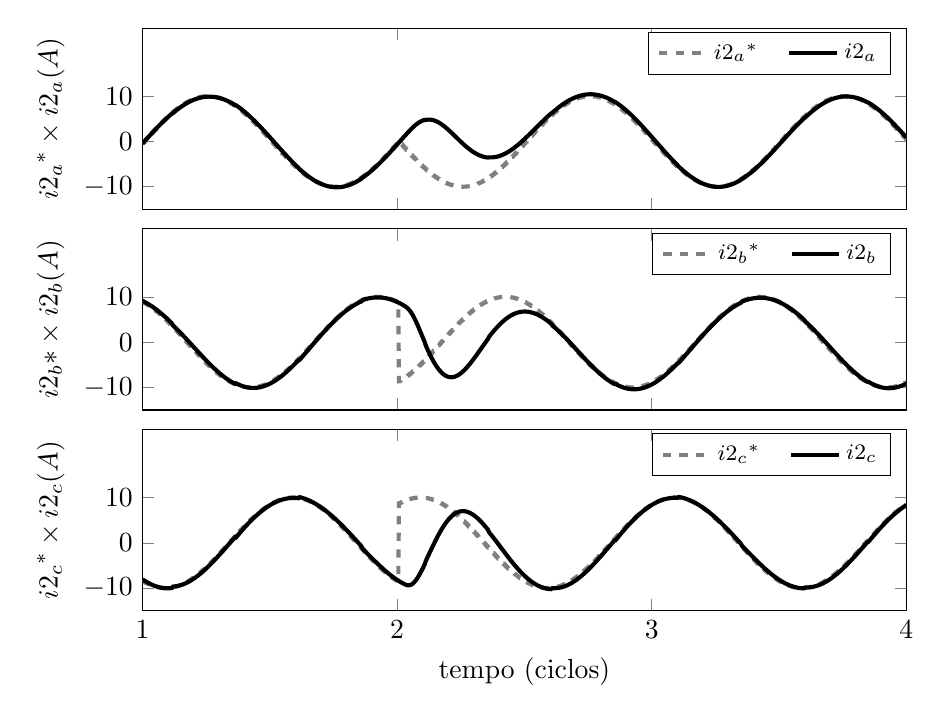
\begin{tikzpicture}

\begin{axis}[%
width=0.8\textwidth,
height=0.189701500343624\textwidth,
scale only axis,
xmin=0.0166666666666667,
xmax=0.0666666666666667,
xtick={0.0166666666666667,0.0333333333333333,0.05,0.0666666666666667},
xticklabels={\empty},
ymin=-15,
ymax=25,
ytick={-10,   0,  10},
ylabel={${\text{i2}_\text{b}}\text{* }\times\text{ i2}_\text{b}\text{ (A)}$},
name=plot2,
legend style={draw=black,fill=white,legend cell align=left},
scaled x ticks = false,
legend columns=-1,
legend style={/tikz/every even column/.append style={column sep=0.3cm}},
legend style={font=\footnotesize}
]
\addplot [color=gray,dashed,line width=1.5pt]
  table[row sep=crcr]{0.0166583333333333	8.95711760239421\\
0.0167	8.81303452065\\
0.0167416666666667	8.81303452065\\
0.0167833333333333	8.66025403784447\\
0.016825	8.66025403784447\\
0.0168666666666667	8.49892692986872\\
0.0169083333333333	8.49892692986872\\
0.01695	8.32921240710107\\
0.0169916666666667	8.32921240710107\\
0.0170333333333333	8.15127795728562\\
0.017075	8.15127795728562\\
0.0171166666666667	7.96529918024204\\
0.0171583333333333	7.96529918024204\\
0.0172	7.77145961456979\\
0.0172416666666667	7.77145961456979\\
0.0172833333333333	7.56995055651764\\
0.017325	7.56995055651764\\
0.0173666666666667	7.36097087119742\\
0.0174083333333333	7.36097087119742\\
0.01745	7.1447267963281\\
0.0174916666666667	7.1447267963281\\
0.0175333333333333	6.92143173870414\\
0.017575	6.92143173870414\\
0.0176166666666667	6.69130606358865\\
0.0176583333333333	6.69130606358865\\
0.0177	6.45457687723957\\
0.0177416666666667	6.45457687723957\\
0.0177833333333333	6.21147780278317\\
0.017825	6.21147780278317\\
0.0178666666666667	5.96224874965622\\
0.0179083333333333	5.96224874965622\\
0.01795	5.70713567684438\\
0.0179916666666667	5.70713567684438\\
0.0180333333333333	5.44639035015033\\
0.018075	5.44639035015033\\
0.0181166666666667	5.18027009373136\\
0.0181583333333333	5.18027009373136\\
0.0182	4.90903753615147\\
0.0182416666666667	4.90903753615147\\
0.0182833333333333	4.63296035119867\\
0.018325	4.63296035119867\\
0.0183666666666667	4.35231099372333\\
0.0184083333333333	4.35231099372333\\
0.01845	4.06736643075805\\
0.0184916666666667	4.06736643075805\\
0.0185333333333333	3.77840786818472\\
0.018575	3.77840786818472\\
0.0186166666666667	3.4857204732182\\
0.0186583333333333	3.4857204732182\\
0.0187	3.18959309298074\\
0.0187416666666667	3.18959309298074\\
0.0187833333333333	2.89031796944476\\
0.018825	2.89031796944476\\
0.0188666666666667	2.58819045102524\\
0.0189083333333333	2.58819045102524\\
0.01895	2.28350870110659\\
0.0189916666666667	2.28350870110659\\
0.0190333333333333	1.97657340379129\\
0.019075	1.97657340379129\\
0.0191166666666667	1.66768746716105\\
0.0191583333333333	1.66768746716105\\
0.0192	1.35715572434307\\
0.0192416666666667	1.35715572434307\\
0.0192833333333333	1.04528463267656\\
0.019325	1.04528463267656\\
0.0193666666666667	0.732381971276336\\
0.0194083333333333	0.732381971276336\\
0.01945	0.418756537292012\\
0.0194916666666667	0.418756537292012\\
0.0195333333333333	0.104717841162471\\
0.019575	0.104717841162471\\
0.0196166666666667	-0.20942419883356\\
0.0196583333333333	-0.20942419883356\\
0.0197	-0.523359562429432\\
0.0197416666666667	-0.523359562429432\\
0.0197833333333333	-0.836778433323152\\
0.019825	-0.836778433323152\\
0.0198666666666667	-1.14937150492867\\
0.0199083333333333	-1.14937150492867\\
0.01995	-1.46083028562412\\
0.0199916666666667	-1.46083028562412\\
0.0200333333333333	-1.77084740319584\\
0.020075	-1.77084740319584\\
0.0201166666666667	-2.0791169081776\\
0.0201583333333333	-2.0791169081776\\
0.0202	-2.38533457578582\\
0.0202416666666667	-2.38533457578582\\
0.0202833333333333	-2.68919820615267\\
0.020325	-2.68919820615267\\
0.0203666666666667	-2.99040792256089\\
0.0204083333333333	-2.99040792256089\\
0.02045	-3.28866646738586\\
0.0204916666666667	-3.28866646738586\\
0.0205333333333333	-3.58367949545303\\
0.020575	-3.58367949545303\\
0.0206166666666667	-3.87515586452106\\
0.0206583333333333	-3.87515586452106\\
0.0207	-4.16280792260405\\
0.0207416666666667	-4.16280792260405\\
0.0207833333333333	-4.44635179184931\\
0.020825	-4.44635179184931\\
0.0208666666666667	-4.72550764869058\\
0.0209083333333333	-4.72550764869058\\
0.02095	-5.00000000000005\\
0.0209916666666667	-5.00000000000005\\
0.0210333333333333	-5.26955795496682\\
0.021075	-5.26955795496682\\
0.0211166666666667	-5.53391549243349\\
0.0211583333333333	-5.53391549243349\\
0.0212	-5.79281172342684\\
0.0212416666666667	-5.79281172342684\\
0.0212833333333333	-6.0459911486238\\
0.021325	-6.0459911486238\\
0.0213666666666667	-6.29320391049844\\
0.0214083333333333	-6.29320391049844\\
0.02145	-6.53420603990112\\
0.0214916666666667	-6.53420603990112\\
0.0215333333333333	-6.76875969682667\\
0.021575	-6.76875969682667\\
0.0216166666666667	-6.99663340513372\\
0.0216583333333333	-6.99663340513372\\
0.0217	-7.2176022809837\\
0.0217416666666667	-7.2176022809837\\
0.0217833333333333	-7.43144825477402\\
0.021825	-7.43144825477402\\
0.0218666666666667	-7.6379602863465\\
0.0219083333333333	-7.6379602863465\\
0.02195	-7.83693457325848\\
0.0219916666666667	-7.83693457325848\\
0.0220333333333333	-8.02817475191123\\
0.022075	-8.02817475191123\\
0.0221166666666667	-8.21149209133713\\
0.0221583333333333	-8.21149209133713\\
0.0222	-8.38670567945433\\
0.0222416666666667	-8.38670567945433\\
0.0222833333333333	-8.55364260160516\\
0.022325	-8.55364260160516\\
0.0223666666666667	-8.71213811120199\\
0.0224083333333333	-8.71213811120199\\
0.02245	-8.86203579231225\\
0.0224916666666667	-8.86203579231225\\
0.0225333333333333	-9.00318771402204\\
0.022575	-9.00318771402204\\
0.0226166666666667	-9.13545457642611\\
0.0226583333333333	-9.13545457642611\\
0.0227	-9.25870584810006\\
0.0227416666666667	-9.25870584810006\\
0.0227833333333333	-9.37281989491902\\
0.022825	-9.37281989491902\\
0.0228666666666667	-9.47768410009597\\
0.0229083333333333	-9.47768410009597\\
0.02295	-9.57319497532079\\
0.0229916666666667	-9.57319497532079\\
0.0230333333333333	-9.6592582628908\\
0.023075	-9.6592582628908\\
0.0231166666666667	-9.73578902873172\\
0.0231583333333333	-9.73578902873172\\
0.0232	-9.80271174621734\\
0.0232416666666667	-9.80271174621734\\
0.0232833333333333	-9.85996037070517\\
0.023325	-9.85996037070517\\
0.0233666666666667	-9.90747840471456\\
0.0234083333333333	-9.90747840471456\\
0.02345	-9.94521895368285\\
0.0234916666666667	-9.94521895368285\\
0.0235333333333333	-9.97314477224471\\
0.023575	-9.97314477224471\\
0.0236166666666667	-9.99122830098871\\
0.0236583333333333	-9.99122830098871\\
0.0237	-9.99945169365525\\
0.0237416666666667	-9.99945169365525\\
0.0237833333333333	-9.99780683474858\\
0.023825	-9.99780683474858\\
0.0238666666666667	-9.98629534754587\\
0.0239083333333333	-9.98629534754587\\
0.02395	-9.96492859249517\\
0.0239916666666667	-9.96492859249517\\
0.0240333333333333	-9.93372765600409\\
0.024075	-9.93372765600409\\
0.0241166666666667	-9.89272332963001\\
0.0241583333333333	-9.89272332963001\\
0.0242	-9.84195607969255\\
0.0242416666666667	-9.84195607969255\\
0.0242833333333333	-9.78147600733818\\
0.024325	-9.78147600733818\\
0.0243666666666667	-9.71134279909649\\
0.0244083333333333	-9.71134279909649\\
0.02445	-9.63162566797671\\
0.0244916666666667	-9.63162566797671\\
0.0245333333333333	-9.5424032851629\\
0.024575	-9.5424032851629\\
0.0246166666666667	-9.44376370237494\\
0.0246583333333333	-9.44376370237494\\
0.0247	-9.33580426497215\\
0.0247416666666667	-9.33580426497215\\
0.0247833333333333	-9.21863151588513\\
0.024825	-9.21863151588513\\
0.0248666666666667	-9.09236109047081\\
0.0249083333333333	-9.09236109047081\\
0.02495	-8.95711760239425\\
0.0249916666666667	-8.95711760239425\\
0.0250333333333333	-8.81303452065005\\
0.025075	-8.81303452065005\\
0.0251166666666667	-8.66025403784451\\
0.0251583333333333	-8.66025403784451\\
0.0252	-8.49892692986876\\
0.0252416666666667	-8.49892692986876\\
0.0252833333333333	-8.32921240710111\\
0.025325	-8.32921240710111\\
0.0253666666666667	-8.15127795728566\\
0.0254083333333333	-8.15127795728566\\
0.02545	-7.96529918024207\\
0.0254916666666667	-7.96529918024207\\
0.0255333333333333	-7.77145961456982\\
0.025575	-7.77145961456982\\
0.0256166666666667	-7.56995055651767\\
0.0256583333333333	-7.56995055651767\\
0.0257	-7.36097087119745\\
0.0257416666666667	-7.36097087119745\\
0.0257833333333333	-7.14472679632814\\
0.025825	-7.14472679632814\\
0.0258666666666667	-6.92143173870417\\
0.0259083333333333	-6.92143173870417\\
0.02595	-6.69130606358868\\
0.0259916666666667	-6.69130606358868\\
0.0260333333333333	-6.4545768772396\\
0.026075	-6.4545768772396\\
0.0261166666666667	-6.2114778027832\\
0.0261583333333333	-6.2114778027832\\
0.0262	-5.96224874965625\\
0.0262416666666667	-5.96224874965625\\
0.0262833333333333	-5.70713567684441\\
0.026325	-5.70713567684441\\
0.0263666666666667	-5.44639035015036\\
0.0264083333333333	-5.44639035015036\\
0.02645	-5.18027009373139\\
0.0264916666666667	-5.18027009373139\\
0.0265333333333333	-4.90903753615149\\
0.026575	-4.90903753615149\\
0.0266166666666667	-4.6329603511987\\
0.0266583333333333	-4.6329603511987\\
0.0267	-4.35231099372335\\
0.0267416666666667	-4.35231099372335\\
0.0267833333333333	-4.06736643075807\\
0.026825	-4.06736643075807\\
0.0268666666666667	-3.77840786818474\\
0.0269083333333333	-3.77840786818474\\
0.02695	-3.48572047321821\\
0.0269916666666667	-3.48572047321821\\
0.0270333333333333	-3.18959309298076\\
0.027075	-3.18959309298076\\
0.0271166666666667	-2.89031796944477\\
0.0271583333333333	-2.89031796944477\\
0.0272	-2.58819045102526\\
0.0272416666666667	-2.58819045102526\\
0.0272833333333333	-2.28350870110661\\
0.027325	-2.28350870110661\\
0.0273666666666667	-1.9765734037913\\
0.0274083333333333	-1.9765734037913\\
0.02745	-1.66768746716106\\
0.0274916666666667	-1.66768746716106\\
0.0275333333333333	-1.35715572434308\\
0.027575	-1.35715572434308\\
0.0276166666666667	-1.04528463267656\\
0.0276583333333333	-1.04528463267656\\
0.0277	-0.732381971276341\\
0.0277416666666667	-0.732381971276341\\
0.0277833333333333	-0.418756537292015\\
0.027825	-0.418756537292015\\
0.0278666666666667	-0.104717841162473\\
0.0279083333333333	-0.104717841162473\\
0.02795	0.209424198833559\\
0.0279916666666667	0.209424198833559\\
0.0280333333333333	0.523359562429433\\
0.028075	0.523359562429433\\
0.0281166666666667	0.836778433323154\\
0.0281583333333333	0.836778433323154\\
0.0282	1.14937150492867\\
0.0282416666666667	1.14937150492867\\
0.0282833333333333	1.46083028562412\\
0.028325	1.46083028562412\\
0.0283666666666667	1.77084740319585\\
0.0284083333333333	1.77084740319585\\
0.02845	2.07911690817761\\
0.0284916666666667	2.07911690817761\\
0.0285333333333333	2.38533457578583\\
0.028575	2.38533457578583\\
0.0286166666666667	2.68919820615268\\
0.0286583333333333	2.68919820615268\\
0.0287	2.9904079225609\\
0.0287416666666667	2.9904079225609\\
0.0287833333333333	3.28866646738587\\
0.028825	3.28866646738587\\
0.0288666666666667	3.58367949545304\\
0.0289083333333333	3.58367949545304\\
0.02895	3.87515586452107\\
0.0289916666666667	3.87515586452107\\
0.0290333333333333	4.16280792260406\\
0.029075	4.16280792260406\\
0.0291166666666667	4.44635179184933\\
0.0291583333333333	4.44635179184933\\
0.0292	4.7255076486906\\
0.0292416666666667	4.7255076486906\\
0.0292833333333333	5.00000000000006\\
0.029325	5.00000000000006\\
0.0293666666666667	5.26955795496684\\
0.0294083333333333	5.26955795496684\\
0.02945	5.53391549243351\\
0.0294916666666667	5.53391549243351\\
0.0295333333333333	5.79281172342686\\
0.029575	5.79281172342686\\
0.0296166666666667	6.04599114862383\\
0.0296583333333333	6.04599114862383\\
0.0297	6.29320391049846\\
0.0297416666666667	6.29320391049846\\
0.0297833333333333	6.53420603990114\\
0.029825	6.53420603990114\\
0.0298666666666667	6.7687596968267\\
0.0299083333333333	6.7687596968267\\
0.02995	6.99663340513375\\
0.0299916666666667	6.99663340513375\\
0.0300333333333333	7.21760228098372\\
0.030075	7.21760228098372\\
0.0301166666666667	7.43144825477405\\
0.0301583333333333	7.43144825477405\\
0.0302	7.63796028634653\\
0.0302416666666667	7.63796028634653\\
0.0302833333333333	7.83693457325851\\
0.030325	7.83693457325851\\
0.0303666666666667	8.02817475191126\\
0.0304083333333333	8.02817475191126\\
0.03045	8.21149209133716\\
0.0304916666666667	8.21149209133716\\
0.0305333333333333	8.38670567945436\\
0.030575	8.38670567945436\\
0.0306166666666667	8.55364260160519\\
0.0306583333333333	8.55364260160519\\
0.0307	8.71213811120203\\
0.0307416666666667	8.71213811120203\\
0.0307833333333333	8.86203579231228\\
0.030825	8.86203579231228\\
0.0308666666666667	9.00318771402207\\
0.0309083333333333	9.00318771402207\\
0.03095	9.13545457642615\\
0.0309916666666667	9.13545457642615\\
0.0310333333333333	9.25870584810009\\
0.031075	9.25870584810009\\
0.0311166666666667	9.37281989491906\\
0.0311583333333333	9.37281989491906\\
0.0312	9.477684100096\\
0.0312416666666667	9.477684100096\\
0.0312833333333333	9.57319497532082\\
0.031325	9.57319497532082\\
0.0313666666666667	9.65925826289084\\
0.0314083333333333	9.65925826289084\\
0.03145	9.73578902873176\\
0.0314916666666667	9.73578902873176\\
0.0315333333333333	9.80271174621738\\
0.031575	9.80271174621738\\
0.0316166666666667	9.85996037070521\\
0.0316583333333333	9.85996037070521\\
0.0317	9.9074784047146\\
0.0317416666666667	9.9074784047146\\
0.0317833333333333	9.94521895368289\\
0.031825	9.94521895368289\\
0.0318666666666667	9.97314477224474\\
0.0319083333333333	9.97314477224474\\
0.03195	9.99122830098875\\
0.0319916666666667	9.99122830098875\\
0.0320333333333333	9.99945169365528\\
0.032075	9.99945169365528\\
0.0321166666666667	9.99780683474862\\
0.0321583333333333	9.99780683474862\\
0.0322	9.98629534754591\\
0.0322416666666667	9.98629534754591\\
0.0322833333333333	9.96492859249521\\
0.032325	9.96492859249521\\
0.0323666666666667	9.93372765600413\\
0.0324083333333333	9.93372765600413\\
0.03245	9.89272332963005\\
0.0324916666666667	9.89272332963005\\
0.0325333333333333	9.84195607969259\\
0.032575	9.84195607969259\\
0.0326166666666667	9.78147600733822\\
0.0326583333333333	9.78147600733822\\
0.0327	9.71134279909653\\
0.0327416666666667	9.71134279909653\\
0.0327833333333333	9.63162566797675\\
0.032825	9.63162566797675\\
0.0328666666666667	9.54240328516294\\
0.0329083333333333	9.54240328516294\\
0.03295	9.44376370237498\\
0.0329916666666667	9.44376370237498\\
0.0330333333333333	9.33580426497218\\
0.033075	9.33580426497218\\
0.0331166666666667	9.21863151588517\\
0.0331583333333333	9.21863151588517\\
0.0332	9.09236109047085\\
0.0332416666666667	9.09236109047085\\
0.0332833333333333	8.95711760239429\\
0.033325	8.95711760239429\\
0.0333666666666667	8.81303452065008\\
0.0334083333333333	8.81303452065008\\
0.03345	-8.66025403784455\\
0.0334916666666667	-8.66025403784455\\
0.0335333333333333	-8.49892692986879\\
0.033575	-8.49892692986879\\
0.0336166666666667	-8.32921240710115\\
0.0336583333333333	-8.32921240710115\\
0.0337	-8.15127795728569\\
0.0337416666666667	-8.15127795728569\\
0.0337833333333333	-7.96529918024211\\
0.033825	-7.96529918024211\\
0.0338666666666667	-7.77145961456986\\
0.0339083333333333	-7.77145961456986\\
0.03395	-7.56995055651771\\
0.0339916666666667	-7.56995055651771\\
0.0340333333333333	-7.36097087119748\\
0.034075	-7.36097087119748\\
0.0341166666666667	-7.14472679632817\\
0.0341583333333333	-7.14472679632817\\
0.0342	-6.9214317387042\\
0.0342416666666667	-6.9214317387042\\
0.0342833333333333	-6.69130606358871\\
0.034325	-6.69130606358871\\
0.0343666666666667	-6.45457687723963\\
0.0344083333333333	-6.45457687723963\\
0.03445	-6.21147780278323\\
0.0344916666666667	-6.21147780278323\\
0.0345333333333333	-5.96224874965628\\
0.034575	-5.96224874965628\\
0.0346166666666667	-5.70713567684443\\
0.0346583333333333	-5.70713567684443\\
0.0347	-5.44639035015038\\
0.0347416666666667	-5.44639035015038\\
0.0347833333333333	-5.18027009373141\\
0.034825	-5.18027009373141\\
0.0348666666666667	-4.90903753615151\\
0.0349083333333333	-4.90903753615151\\
0.03495	-4.63296035119872\\
0.0349916666666667	-4.63296035119872\\
0.0350333333333333	-4.35231099372337\\
0.035075	-4.35231099372337\\
0.0351166666666667	-4.06736643075809\\
0.0351583333333333	-4.06736643075809\\
0.0352	-3.77840786818476\\
0.0352416666666667	-3.77840786818476\\
0.0352833333333333	-3.48572047321823\\
0.035325	-3.48572047321823\\
0.0353666666666667	-3.18959309298077\\
0.0354083333333333	-3.18959309298077\\
0.03545	-2.89031796944478\\
0.0354916666666667	-2.89031796944478\\
0.0355333333333333	-2.58819045102527\\
0.035575	-2.58819045102527\\
0.0356166666666667	-2.28350870110662\\
0.0356583333333333	-2.28350870110662\\
0.0357	-1.97657340379131\\
0.0357416666666667	-1.97657340379131\\
0.0357833333333333	-1.66768746716107\\
0.035825	-1.66768746716107\\
0.0358666666666667	-1.35715572434309\\
0.0359083333333333	-1.35715572434309\\
0.03595	-1.04528463267657\\
0.0359916666666667	-1.04528463267657\\
0.0360333333333333	-0.732381971276348\\
0.036075	-0.732381971276348\\
0.0361166666666667	-0.418756537292022\\
0.0361583333333333	-0.418756537292022\\
0.0362	-0.104717841162477\\
0.0362416666666667	-0.104717841162477\\
0.0362833333333333	0.209424198833557\\
0.036325	0.209424198833557\\
0.0363666666666667	0.523359562429431\\
0.0364083333333333	0.523359562429431\\
0.03645	0.836778433323154\\
0.0364916666666667	0.836778433323154\\
0.0365333333333333	1.14937150492867\\
0.036575	1.14937150492867\\
0.0366166666666667	1.46083028562413\\
0.0366583333333333	1.46083028562413\\
0.0367	1.77084740319585\\
0.0367416666666667	1.77084740319585\\
0.0367833333333333	2.07911690817762\\
0.036825	2.07911690817762\\
0.0368666666666667	2.38533457578584\\
0.0369083333333333	2.38533457578584\\
0.03695	2.68919820615269\\
0.0369916666666667	2.68919820615269\\
0.0370333333333333	2.99040792256091\\
0.037075	2.99040792256091\\
0.0371166666666667	3.28866646738588\\
0.0371583333333333	3.28866646738588\\
0.0372	3.58367949545306\\
0.0372416666666667	3.58367949545306\\
0.0372833333333333	3.87515586452109\\
0.037325	3.87515586452109\\
0.0373666666666667	4.16280792260408\\
0.0374083333333333	4.16280792260408\\
0.03745	4.44635179184934\\
0.0374916666666667	4.44635179184934\\
0.0375333333333333	4.72550764869062\\
0.037575	4.72550764869062\\
0.0376166666666667	5.00000000000008\\
0.0376583333333333	5.00000000000008\\
0.0377	5.26955795496686\\
0.0377416666666667	5.26955795496686\\
0.0377833333333333	5.53391549243353\\
0.037825	5.53391549243353\\
0.0378666666666667	5.79281172342689\\
0.0379083333333333	5.79281172342689\\
0.03795	6.04599114862385\\
0.0379916666666667	6.04599114862385\\
0.0380333333333333	6.29320391049848\\
0.038075	6.29320391049848\\
0.0381166666666667	6.53420603990117\\
0.0381583333333333	6.53420603990117\\
0.0382	6.76875969682673\\
0.0382416666666667	6.76875969682673\\
0.0382833333333333	6.99663340513378\\
0.038325	6.99663340513378\\
0.0383666666666667	7.21760228098375\\
0.0384083333333333	7.21760228098375\\
0.03845	7.43144825477408\\
0.0384916666666667	7.43144825477408\\
0.0385333333333333	7.63796028634656\\
0.038575	7.63796028634656\\
0.0386166666666667	7.83693457325854\\
0.0386583333333333	7.83693457325854\\
0.0387	8.02817475191129\\
0.0387416666666667	8.02817475191129\\
0.0387833333333333	8.21149209133719\\
0.038825	8.21149209133719\\
0.0388666666666667	8.3867056794544\\
0.0389083333333333	8.3867056794544\\
0.03895	8.55364260160523\\
0.0389916666666667	8.55364260160523\\
0.0390333333333333	8.71213811120206\\
0.039075	8.71213811120206\\
0.0391166666666667	8.86203579231232\\
0.0391583333333333	8.86203579231232\\
0.0392	9.00318771402211\\
0.0392416666666667	9.00318771402211\\
0.0392833333333333	9.13545457642618\\
0.039325	9.13545457642618\\
0.0393666666666667	9.25870584810013\\
0.0394083333333333	9.25870584810013\\
0.03945	9.3728198949191\\
0.0394916666666667	9.3728198949191\\
0.0395333333333333	9.47768410009604\\
0.039575	9.47768410009604\\
0.0396166666666667	9.57319497532086\\
0.0396583333333333	9.57319497532086\\
0.0397	9.65925826289087\\
0.0397416666666667	9.65925826289087\\
0.0397833333333333	9.7357890287318\\
0.039825	9.7357890287318\\
0.0398666666666667	9.80271174621742\\
0.0399083333333333	9.80271174621742\\
0.03995	9.85996037070525\\
0.0399916666666667	9.85996037070525\\
0.0400333333333333	9.90747840471464\\
0.040075	9.90747840471464\\
0.0401166666666667	9.94521895368294\\
0.0401583333333333	9.94521895368294\\
0.0402	9.97314477224478\\
0.0402416666666667	9.97314477224478\\
0.0402833333333333	9.99122830098879\\
0.040325	9.99122830098879\\
0.0403666666666667	9.99945169365533\\
0.0404083333333333	9.99945169365533\\
0.04045	9.99780683474866\\
0.0404916666666667	9.99780683474866\\
0.0405333333333333	9.98629534754595\\
0.040575	9.98629534754595\\
0.0406166666666667	9.96492859249525\\
0.0406583333333333	9.96492859249525\\
0.0407	9.93372765600417\\
0.0407416666666667	9.93372765600417\\
0.0407833333333333	9.89272332963009\\
0.040825	9.89272332963009\\
0.0408666666666667	9.84195607969263\\
0.0409083333333333	9.84195607969263\\
0.04095	9.78147600733827\\
0.0409916666666667	9.78147600733827\\
0.0410333333333333	9.71134279909657\\
0.041075	9.71134279909657\\
0.0411166666666667	9.63162566797679\\
0.0411583333333333	9.63162566797679\\
0.0412	9.54240328516298\\
0.0412416666666667	9.54240328516298\\
0.0412833333333333	9.44376370237502\\
0.041325	9.44376370237502\\
0.0413666666666667	9.33580426497222\\
0.0414083333333333	9.33580426497222\\
0.04145	9.21863151588521\\
0.0414916666666667	9.21863151588521\\
0.0415333333333333	9.09236109047089\\
0.041575	9.09236109047089\\
0.0416166666666667	8.95711760239433\\
0.0416583333333333	8.95711760239433\\
0.0417	8.81303452065012\\
0.0417416666666667	8.81303452065012\\
0.0417833333333333	8.66025403784458\\
0.041825	8.66025403784458\\
0.0418666666666667	8.49892692986883\\
0.0419083333333333	8.49892692986883\\
0.04195	8.32921240710118\\
0.0419916666666667	8.32921240710118\\
0.0420333333333333	8.15127795728573\\
0.042075	8.15127795728573\\
0.0421166666666667	7.96529918024214\\
0.0421583333333333	7.96529918024214\\
0.0422	7.77145961456989\\
0.0422416666666667	7.77145961456989\\
0.0422833333333333	7.56995055651774\\
0.042325	7.56995055651774\\
0.0423666666666667	7.36097087119751\\
0.0424083333333333	7.36097087119751\\
0.04245	7.1447267963282\\
0.0424916666666667	7.1447267963282\\
0.0425333333333333	6.92143173870423\\
0.042575	6.92143173870423\\
0.0426166666666667	6.69130606358874\\
0.0426583333333333	6.69130606358874\\
0.0427	6.45457687723966\\
0.0427416666666667	6.45457687723966\\
0.0427833333333333	6.21147780278325\\
0.042825	6.21147780278325\\
0.0428666666666667	5.9622487496563\\
0.0429083333333333	5.9622487496563\\
0.04295	5.70713567684446\\
0.0429916666666667	5.70713567684446\\
0.0430333333333333	5.44639035015041\\
0.043075	5.44639035015041\\
0.0431166666666667	5.18027009373143\\
0.0431583333333333	5.18027009373143\\
0.0432	4.90903753615153\\
0.0432416666666667	4.90903753615153\\
0.0432833333333333	4.63296035119874\\
0.043325	4.63296035119874\\
0.0433666666666667	4.35231099372339\\
0.0434083333333333	4.35231099372339\\
0.04345	4.06736643075811\\
0.0434916666666667	4.06736643075811\\
0.0435333333333333	3.77840786818477\\
0.043575	3.77840786818477\\
0.0436166666666667	3.48572047321825\\
0.0436583333333333	3.48572047321825\\
0.0437	3.18959309298079\\
0.0437416666666667	3.18959309298079\\
0.0437833333333333	2.8903179694448\\
0.043825	2.8903179694448\\
0.0438666666666667	2.58819045102528\\
0.0439083333333333	2.58819045102528\\
0.04395	2.28350870110663\\
0.0439916666666667	2.28350870110663\\
0.0440333333333333	1.97657340379133\\
0.044075	1.97657340379133\\
0.0441166666666667	1.66768746716108\\
0.0441583333333333	1.66768746716108\\
0.0442	1.35715572434309\\
0.0442416666666667	1.35715572434309\\
0.0442833333333333	1.04528463267658\\
0.044325	1.04528463267658\\
0.0443666666666667	0.732381971276353\\
0.0444083333333333	0.732381971276353\\
0.04445	0.418756537292025\\
0.0444916666666667	0.418756537292025\\
0.0445333333333333	0.104717841162479\\
0.044575	0.104717841162479\\
0.0446166666666667	-0.209424198833555\\
0.0446583333333333	-0.209424198833555\\
0.0447	-0.523359562429432\\
0.0447416666666667	-0.523359562429432\\
0.0447833333333333	-0.836778433323156\\
0.044825	-0.836778433323156\\
0.0448666666666667	-1.14937150492867\\
0.0449083333333333	-1.14937150492867\\
0.04495	-1.46083028562413\\
0.0449916666666667	-1.46083028562413\\
0.0450333333333333	-1.77084740319586\\
0.045075	-1.77084740319586\\
0.0451166666666667	-2.07911690817762\\
0.0451583333333333	-2.07911690817762\\
0.0452	-2.38533457578585\\
0.0452416666666667	-2.38533457578585\\
0.0452833333333333	-2.6891982061527\\
0.045325	-2.6891982061527\\
0.0453666666666667	-2.99040792256092\\
0.0454083333333333	-2.99040792256092\\
0.04545	-3.28866646738589\\
0.0454916666666667	-3.28866646738589\\
0.0455333333333333	-3.58367949545307\\
0.045575	-3.58367949545307\\
0.0456166666666667	-3.8751558645211\\
0.0456583333333333	-3.8751558645211\\
0.0457	-4.16280792260409\\
0.0457416666666667	-4.16280792260409\\
0.0457833333333333	-4.44635179184936\\
0.045825	-4.44635179184936\\
0.0458666666666667	-4.72550764869064\\
0.0459083333333333	-4.72550764869064\\
0.04595	-5.0000000000001\\
0.0459916666666667	-5.0000000000001\\
0.0460333333333333	-5.26955795496689\\
0.046075	-5.26955795496689\\
0.0461166666666667	-5.53391549243356\\
0.0461583333333333	-5.53391549243356\\
0.0462	-5.79281172342691\\
0.0462416666666667	-5.79281172342691\\
0.0462833333333333	-6.04599114862388\\
0.046325	-6.04599114862388\\
0.0463666666666667	-6.29320391049851\\
0.0464083333333333	-6.29320391049851\\
0.04645	-6.5342060399012\\
0.0464916666666667	-6.5342060399012\\
0.0465333333333333	-6.76875969682676\\
0.046575	-6.76875969682676\\
0.0466166666666667	-6.99663340513381\\
0.0466583333333333	-6.99663340513381\\
0.0467	-7.21760228098379\\
0.0467416666666667	-7.21760228098379\\
0.0467833333333333	-7.43144825477411\\
0.046825	-7.43144825477411\\
0.0468666666666667	-7.6379602863466\\
0.0469083333333333	-7.6379602863466\\
0.04695	-7.83693457325858\\
0.0469916666666667	-7.83693457325858\\
0.0470333333333333	-8.02817475191133\\
0.047075	-8.02817475191133\\
0.0471166666666667	-8.21149209133723\\
0.0471583333333333	-8.21149209133723\\
0.0472	-8.38670567945444\\
0.0472416666666667	-8.38670567945444\\
0.0472833333333333	-8.55364260160527\\
0.047325	-8.55364260160527\\
0.0473666666666667	-8.7121381112021\\
0.0474083333333333	-8.7121381112021\\
0.04745	-8.86203579231236\\
0.0474916666666667	-8.86203579231236\\
0.0475333333333333	-9.00318771402215\\
0.047575	-9.00318771402215\\
0.0476166666666667	-9.13545457642623\\
0.0476583333333333	-9.13545457642623\\
0.0477	-9.25870584810017\\
0.0477416666666667	-9.25870584810017\\
0.0477833333333333	-9.37281989491914\\
0.047825	-9.37281989491914\\
0.0478666666666667	-9.47768410009609\\
0.0479083333333333	-9.47768410009609\\
0.04795	-9.57319497532091\\
0.0479916666666667	-9.57319497532091\\
0.0480333333333333	-9.65925826289092\\
0.048075	-9.65925826289092\\
0.0481166666666667	-9.73578902873184\\
0.0481583333333333	-9.73578902873184\\
0.0482	-9.80271174621746\\
0.0482416666666667	-9.80271174621746\\
0.0482833333333333	-9.85996037070529\\
0.048325	-9.85996037070529\\
0.0483666666666667	-9.90747840471468\\
0.0484083333333333	-9.90747840471468\\
0.04845	-9.94521895368298\\
0.0484916666666667	-9.94521895368298\\
0.0485333333333333	-9.97314477224483\\
0.048575	-9.97314477224483\\
0.0486166666666667	-9.99122830098883\\
0.0486583333333333	-9.99122830098883\\
0.0487	-9.99945169365537\\
0.0487416666666667	-9.99945169365537\\
0.0487833333333333	-9.99780683474871\\
0.048825	-9.99780683474871\\
0.0488666666666667	-9.98629534754599\\
0.0489083333333333	-9.98629534754599\\
0.04895	-9.9649285924953\\
0.0489916666666667	-9.9649285924953\\
0.0490333333333333	-9.93372765600422\\
0.049075	-9.93372765600422\\
0.0491166666666667	-9.89272332963014\\
0.0491583333333333	-9.89272332963014\\
0.0492	-9.84195607969268\\
0.0492416666666667	-9.84195607969268\\
0.0492833333333333	-9.78147600733831\\
0.049325	-9.78147600733831\\
0.0493666666666667	-9.71134279909661\\
0.0494083333333333	-9.71134279909661\\
0.04945	-9.63162566797684\\
0.0494916666666667	-9.63162566797684\\
0.0495333333333333	-9.54240328516302\\
0.049575	-9.54240328516302\\
0.0496166666666667	-9.44376370237506\\
0.0496583333333333	-9.44376370237506\\
0.0497	-9.33580426497227\\
0.0497416666666667	-9.33580426497227\\
0.0497833333333333	-9.21863151588525\\
0.049825	-9.21863151588525\\
0.0498666666666667	-9.09236109047093\\
0.0499083333333333	-9.09236109047093\\
0.04995	-8.95711760239437\\
0.0499916666666667	-8.95711760239437\\
0.0500333333333333	-8.81303452065016\\
0.050075	-8.81303452065016\\
0.0501166666666667	-8.66025403784462\\
0.0501583333333333	-8.66025403784462\\
0.0502	-8.49892692986887\\
0.0502416666666667	-8.49892692986887\\
0.0502833333333333	-8.32921240710123\\
0.050325	-8.32921240710123\\
0.0503666666666667	-8.15127795728577\\
0.0504083333333333	-8.15127795728577\\
0.05045	-7.96529918024218\\
0.0504916666666667	-7.96529918024218\\
0.0505333333333333	-7.77145961456993\\
0.050575	-7.77145961456993\\
0.0506166666666667	-7.56995055651778\\
0.0506583333333333	-7.56995055651778\\
0.0507	-7.36097087119755\\
0.0507416666666667	-7.36097087119755\\
0.0507833333333333	-7.14472679632824\\
0.050825	-7.14472679632824\\
0.0508666666666667	-6.92143173870427\\
0.0509083333333333	-6.92143173870427\\
0.05095	-6.69130606358878\\
0.0509916666666667	-6.69130606358878\\
0.0510333333333333	-6.45457687723969\\
0.051075	-6.45457687723969\\
0.0511166666666667	-6.21147780278329\\
0.0511583333333333	-6.21147780278329\\
0.0512	-5.96224874965633\\
0.0512416666666667	-5.96224874965633\\
0.0512833333333333	-5.70713567684449\\
0.051325	-5.70713567684449\\
0.0513666666666667	-5.44639035015043\\
0.0514083333333333	-5.44639035015043\\
0.05145	-5.18027009373146\\
0.0514916666666667	-5.18027009373146\\
0.0515333333333333	-4.90903753615156\\
0.051575	-4.90903753615156\\
0.0516166666666667	-4.63296035119876\\
0.0516583333333333	-4.63296035119876\\
0.0517	-4.35231099372341\\
0.0517416666666667	-4.35231099372341\\
0.0517833333333333	-4.06736643075813\\
0.051825	-4.06736643075813\\
0.0518666666666667	-3.77840786818479\\
0.0519083333333333	-3.77840786818479\\
0.05195	-3.48572047321827\\
0.0519916666666667	-3.48572047321827\\
0.0520333333333333	-3.18959309298081\\
0.052075	-3.18959309298081\\
0.0521166666666667	-2.89031796944481\\
0.0521583333333333	-2.89031796944481\\
0.0522	-2.5881904510253\\
0.0522416666666667	-2.5881904510253\\
0.0522833333333333	-2.28350870110664\\
0.052325	-2.28350870110664\\
0.0523666666666667	-1.97657340379134\\
0.0524083333333333	-1.97657340379134\\
0.05245	-1.66768746716109\\
0.0524916666666667	-1.66768746716109\\
0.0525333333333333	-1.3571557243431\\
0.052575	-1.3571557243431\\
0.0526166666666667	-1.04528463267659\\
0.0526583333333333	-1.04528463267659\\
0.0527	-0.73238197127636\\
0.0527416666666667	-0.73238197127636\\
0.0527833333333333	-0.418756537292029\\
0.052825	-0.418756537292029\\
0.0528666666666667	-0.104717841162482\\
0.0529083333333333	-0.104717841162482\\
0.05295	0.209424198833554\\
0.0529916666666667	0.209424198833554\\
0.0530333333333333	0.523359562429432\\
0.053075	0.523359562429432\\
0.0531166666666667	0.836778433323157\\
0.0531583333333333	0.836778433323157\\
0.0532	1.14937150492868\\
0.0532416666666667	1.14937150492868\\
0.0532833333333333	1.46083028562414\\
0.053325	1.46083028562414\\
0.0533666666666667	1.77084740319586\\
0.0534083333333333	1.77084740319586\\
0.05345	2.07911690817763\\
0.0534916666666667	2.07911690817763\\
0.0535333333333333	2.38533457578585\\
0.053575	2.38533457578585\\
0.0536166666666667	2.68919820615271\\
0.0536583333333333	2.68919820615271\\
0.0537	2.99040792256093\\
0.0537416666666667	2.99040792256093\\
0.0537833333333333	3.2886664673859\\
0.053825	3.2886664673859\\
0.0538666666666667	3.58367949545308\\
0.0539083333333333	3.58367949545308\\
0.05395	3.87515586452112\\
0.0539916666666667	3.87515586452112\\
0.0540333333333333	4.16280792260411\\
0.054075	4.16280792260411\\
0.0541166666666667	4.44635179184938\\
0.0541583333333333	4.44635179184938\\
0.0542	4.72550764869065\\
0.0542416666666667	4.72550764869065\\
0.0542833333333333	5.00000000000012\\
0.054325	5.00000000000012\\
0.0543666666666667	5.26955795496691\\
0.0544083333333333	5.26955795496691\\
0.05445	5.53391549243358\\
0.0544916666666667	5.53391549243358\\
0.0545333333333333	5.79281172342693\\
0.054575	5.79281172342693\\
0.0546166666666667	6.0459911486239\\
0.0546583333333333	6.0459911486239\\
0.0547	6.29320391049854\\
0.0547416666666667	6.29320391049854\\
0.0547833333333333	6.53420603990122\\
0.054825	6.53420603990122\\
0.0548666666666667	6.76875969682678\\
0.0549083333333333	6.76875969682678\\
0.05495	6.99663340513384\\
0.0549916666666667	6.99663340513384\\
0.0550333333333333	7.21760228098381\\
0.055075	7.21760228098381\\
0.0551166666666667	7.43144825477414\\
0.0551583333333333	7.43144825477414\\
0.0552	7.63796028634663\\
0.0552416666666667	7.63796028634663\\
0.0552833333333333	7.83693457325861\\
0.055325	7.83693457325861\\
0.0553666666666667	8.02817475191136\\
0.0554083333333333	8.02817475191136\\
0.05545	8.21149209133726\\
0.0554916666666667	8.21149209133726\\
0.0555333333333333	8.38670567945447\\
0.055575	8.38670567945447\\
0.0556166666666667	8.5536426016053\\
0.0556583333333333	8.5536426016053\\
0.0557	8.71213811120214\\
0.0557416666666667	8.71213811120214\\
0.0557833333333333	8.86203579231239\\
0.055825	8.86203579231239\\
0.0558666666666667	9.00318771402219\\
0.0559083333333333	9.00318771402219\\
0.05595	9.13545457642627\\
0.0559916666666667	9.13545457642627\\
0.0560333333333333	9.25870584810021\\
0.056075	9.25870584810021\\
0.0561166666666667	9.37281989491918\\
0.0561583333333333	9.37281989491918\\
0.0562	9.47768410009613\\
0.0562416666666667	9.47768410009613\\
0.0562833333333333	9.57319497532095\\
0.056325	9.57319497532095\\
0.0563666666666667	9.65925826289096\\
0.0564083333333333	9.65925826289096\\
0.05645	9.73578902873188\\
0.0564916666666667	9.73578902873188\\
0.0565333333333333	9.8027117462175\\
0.056575	9.8027117462175\\
0.0566166666666667	9.85996037070534\\
0.0566583333333333	9.85996037070534\\
0.0567	9.90747840471473\\
0.0567416666666667	9.90747840471473\\
0.0567833333333333	9.94521895368302\\
0.056825	9.94521895368302\\
0.0568666666666667	9.97314477224487\\
0.0569083333333333	9.97314477224487\\
0.05695	9.99122830098888\\
0.0569916666666667	9.99122830098888\\
0.0570333333333333	9.99945169365542\\
0.057075	9.99945169365542\\
0.0571166666666667	9.99780683474875\\
0.0571583333333333	9.99780683474875\\
0.0572	9.98629534754604\\
0.0572416666666667	9.98629534754604\\
0.0572833333333333	9.96492859249534\\
0.057325	9.96492859249534\\
0.0573666666666667	9.93372765600427\\
0.0574083333333333	9.93372765600427\\
0.05745	9.89272332963018\\
0.0574916666666667	9.89272332963018\\
0.0575333333333333	9.84195607969272\\
0.057575	9.84195607969272\\
0.0576166666666667	9.78147600733836\\
0.0576583333333333	9.78147600733836\\
0.0577	9.71134279909666\\
0.0577416666666667	9.71134279909666\\
0.0577833333333333	9.63162566797688\\
0.057825	9.63162566797688\\
0.0578666666666667	9.54240328516306\\
0.0579083333333333	9.54240328516306\\
0.05795	9.44376370237511\\
0.0579916666666667	9.44376370237511\\
0.0580333333333333	9.33580426497231\\
0.058075	9.33580426497231\\
0.0581166666666667	9.21863151588529\\
0.0581583333333333	9.21863151588529\\
0.0582	9.09236109047097\\
0.0582416666666667	9.09236109047097\\
0.0582833333333333	8.95711760239441\\
0.058325	8.95711760239441\\
0.0583666666666667	8.8130345206502\\
0.0584083333333333	8.8130345206502\\
0.05845	8.66025403784466\\
0.0584916666666667	8.66025403784466\\
0.0585333333333333	8.49892692986891\\
0.058575	8.49892692986891\\
0.0586166666666667	8.32921240710126\\
0.0586583333333333	8.32921240710126\\
0.0587	8.1512779572858\\
0.0587416666666667	8.1512779572858\\
0.0587833333333333	7.96529918024222\\
0.058825	7.96529918024222\\
0.0588666666666667	7.77145961456996\\
0.0589083333333333	7.77145961456996\\
0.05895	7.56995055651781\\
0.0589916666666667	7.56995055651781\\
0.0590333333333333	7.36097087119758\\
0.059075	7.36097087119758\\
0.0591166666666667	7.14472679632827\\
0.0591583333333333	7.14472679632827\\
0.0592	6.9214317387043\\
0.0592416666666667	6.9214317387043\\
0.0592833333333333	6.69130606358881\\
0.059325	6.69130606358881\\
0.0593666666666667	6.45457687723972\\
0.0594083333333333	6.45457687723972\\
0.05945	6.21147780278331\\
0.0594916666666667	6.21147780278331\\
0.0595333333333333	5.96224874965636\\
0.059575	5.96224874965636\\
0.0596166666666667	5.70713567684451\\
0.0596583333333333	5.70713567684451\\
0.0597	5.44639035015046\\
0.0597416666666667	5.44639035015046\\
0.0597833333333333	5.18027009373148\\
0.059825	5.18027009373148\\
0.0598666666666667	4.90903753615158\\
0.0599083333333333	4.90903753615158\\
0.05995	4.63296035119878\\
0.0599916666666667	4.63296035119878\\
0.0600333333333333	4.35231099372343\\
0.060075	4.35231099372343\\
0.0601166666666667	4.06736643075815\\
0.0601583333333333	4.06736643075815\\
0.0602	3.77840786818481\\
0.0602416666666667	3.77840786818481\\
0.0602833333333333	3.48572047321828\\
0.060325	3.48572047321828\\
0.0603666666666667	3.18959309298082\\
0.0604083333333333	3.18959309298082\\
0.06045	2.89031796944483\\
0.0604916666666667	2.89031796944483\\
0.0605333333333333	2.58819045102531\\
0.060575	2.58819045102531\\
0.0606166666666667	2.28350870110665\\
0.0606583333333333	2.28350870110665\\
0.0607	1.97657340379135\\
0.0607416666666667	1.97657340379135\\
0.0607833333333333	1.6676874671611\\
0.060825	1.6676874671611\\
0.0608666666666667	1.35715572434311\\
0.0609083333333333	1.35715572434311\\
0.06095	1.04528463267659\\
0.0609916666666667	1.04528463267659\\
0.0610333333333333	0.732381971276366\\
0.061075	0.732381971276366\\
0.0611166666666667	0.418756537292034\\
0.0611583333333333	0.418756537292034\\
0.0612	0.104717841162486\\
0.0612416666666667	0.104717841162486\\
0.0612833333333333	-0.209424198833552\\
0.061325	-0.209424198833552\\
0.0613666666666667	-0.52335956242943\\
0.0614083333333333	-0.52335956242943\\
0.06145	-0.836778433323157\\
0.0614916666666667	-0.836778433323157\\
0.0615333333333333	-1.14937150492868\\
0.061575	-1.14937150492868\\
0.0616166666666667	-1.46083028562414\\
0.0616583333333333	-1.46083028562414\\
0.0617	-1.77084740319587\\
0.0617416666666667	-1.77084740319587\\
0.0617833333333333	-2.07911690817764\\
0.061825	-2.07911690817764\\
0.0618666666666667	-2.38533457578586\\
0.0619083333333333	-2.38533457578586\\
0.06195	-2.68919820615272\\
0.0619916666666667	-2.68919820615272\\
0.0620333333333333	-2.99040792256094\\
0.062075	-2.99040792256094\\
0.0621166666666667	-3.28866646738591\\
0.0621583333333333	-3.28866646738591\\
0.0622	-3.5836794954531\\
0.0622416666666667	-3.5836794954531\\
0.0622833333333333	-3.87515586452113\\
0.062325	-3.87515586452113\\
0.0623666666666667	-4.16280792260412\\
0.0624083333333333	-4.16280792260412\\
0.06245	-4.4463517918494\\
0.0624916666666667	-4.4463517918494\\
0.0625333333333333	-4.72550764869067\\
0.062575	-4.72550764869067\\
0.0626166666666667	-5.00000000000014\\
0.0626583333333333	-5.00000000000014\\
0.0627	-5.26955795496693\\
0.0627416666666667	-5.26955795496693\\
0.0627833333333333	-5.5339154924336\\
0.062825	-5.5339154924336\\
0.0628666666666667	-5.79281172342696\\
0.0629083333333333	-5.79281172342696\\
0.06295	-6.04599114862392\\
0.0629916666666667	-6.04599114862392\\
0.0630333333333333	-6.29320391049856\\
0.063075	-6.29320391049856\\
0.0631166666666667	-6.53420603990125\\
0.0631583333333333	-6.53420603990125\\
0.0632	-6.76875969682681\\
0.0632416666666667	-6.76875969682681\\
0.0632833333333333	-6.99663340513387\\
0.063325	-6.99663340513387\\
0.0633666666666667	-7.21760228098384\\
0.0634083333333333	-7.21760228098384\\
0.06345	-7.43144825477417\\
0.0634916666666667	-7.43144825477417\\
0.0635333333333333	-7.63796028634666\\
0.063575	-7.63796028634666\\
0.0636166666666667	-7.83693457325864\\
0.0636583333333333	-7.83693457325864\\
0.0637	-8.0281747519114\\
0.0637416666666667	-8.0281747519114\\
0.0637833333333333	-8.2114920913373\\
0.063825	-8.2114920913373\\
0.0638666666666667	-8.3867056794545\\
0.0639083333333333	-8.3867056794545\\
0.06395	-8.55364260160534\\
0.0639916666666667	-8.55364260160534\\
0.0640333333333333	-8.71213811120217\\
0.064075	-8.71213811120217\\
0.0641166666666667	-8.86203579231243\\
0.0641583333333333	-8.86203579231243\\
0.0642	-9.00318771402222\\
0.0642416666666667	-9.00318771402222\\
0.0642833333333333	-9.1354545764263\\
0.064325	-9.1354545764263\\
0.0643666666666667	-9.25870584810025\\
0.0644083333333333	-9.25870584810025\\
0.06445	-9.37281989491922\\
0.0644916666666667	-9.37281989491922\\
0.0645333333333333	-9.47768410009616\\
0.064575	-9.47768410009616\\
0.0646166666666667	-9.57319497532098\\
0.0646583333333333	-9.57319497532098\\
0.0647	-9.659258262891\\
0.0647416666666667	-9.659258262891\\
0.0647833333333333	-9.73578902873192\\
0.064825	-9.73578902873192\\
0.0648666666666667	-9.80271174621754\\
0.0649083333333333	-9.80271174621754\\
0.06495	-9.85996037070537\\
0.0649916666666667	-9.85996037070537\\
0.0650333333333333	-9.90747840471476\\
0.065075	-9.90747840471476\\
0.0651166666666667	-9.94521895368306\\
0.0651583333333333	-9.94521895368306\\
0.0652	-9.97314477224491\\
0.0652416666666667	-9.97314477224491\\
0.0652833333333333	-9.99122830098892\\
0.065325	-9.99122830098892\\
0.0653666666666667	-9.99945169365546\\
0.0654083333333333	-9.99945169365546\\
0.06545	-9.99780683474879\\
0.0654916666666667	-9.99780683474879\\
0.0655333333333333	-9.98629534754607\\
0.065575	-9.98629534754607\\
0.0656166666666667	-9.96492859249538\\
0.0656583333333333	-9.96492859249538\\
0.0657	-9.9337276560043\\
0.0657416666666667	-9.9337276560043\\
0.0657833333333333	-9.89272332963022\\
0.065825	-9.89272332963022\\
0.0658666666666667	-9.84195607969276\\
0.0659083333333333	-9.84195607969276\\
0.06595	-9.78147600733839\\
0.0659916666666667	-9.78147600733839\\
0.0660333333333333	-9.71134279909669\\
0.066075	-9.71134279909669\\
0.0661166666666667	-9.63162566797691\\
0.0661583333333333	-9.63162566797691\\
0.0662	-9.5424032851631\\
0.0662416666666667	-9.5424032851631\\
0.0662833333333333	-9.44376370237514\\
0.066325	-9.44376370237514\\
0.0663666666666667	-9.33580426497234\\
0.0664083333333333	-9.33580426497234\\
0.06645	-9.21863151588533\\
0.0664916666666667	-9.21863151588533\\
0.0665333333333333	-9.092361090471\\
0.066575	-9.092361090471\\
0.0666166666666667	-8.95711760239444\\
0.0666583333333333	-8.95711760239444\\
};
\addlegendentry{${\text{i2}_\text{b}}^\text{*}$};

\addplot [color=black,solid,line width=1.5pt]
  table[row sep=crcr]{0.0166583333333333	9.10238729436972\\
0.0167	9.03402165826534\\
0.0167416666666667	8.96368598655141\\
0.0167833333333333	8.89133568061203\\
0.016825	8.81704993622876\\
0.0168666666666667	8.74079343507884\\
0.0169083333333333	8.66265295711749\\
0.01695	8.58259781627092\\
0.0169916666666667	8.50071754137033\\
0.0170333333333333	8.41698140145812\\
0.017075	8.33147777016323\\
0.0171166666666667	8.24417239647427\\
0.0171583333333333	8.15515004140646\\
0.0172	8.06437114911801\\
0.0172416666666667	7.97191608287754\\
0.0172833333333333	7.8777397886972\\
0.017325	7.7819187867049\\
0.0173666666666667	7.68440342410503\\
0.0174083333333333	7.58526770699698\\
0.01745	7.48445879295424\\
0.0174916666666667	7.38204974177135\\
0.0175333333333333	7.27798597031744\\
0.017575	7.1723588885292\\
0.0176166666666667	7.06511633678431\\
0.0176583333333333	6.95626978050029\\
0.0177	6.84580684667755\\
0.0177416666666667	6.73380549079232\\
0.0177833333333333	6.62021165288726\\
0.017825	6.50510560395105\\
0.0178666666666667	6.38843437691671\\
0.0179083333333333	6.2702810790216\\
0.01795	6.15059383602935\\
0.0179916666666667	6.02945861112754\\
0.0180333333333333	5.9068245245065\\
0.018075	5.78278034407908\\
0.0181166666666667	5.65727605146901\\
0.0181583333333333	5.53040314356191\\
0.0182	5.40211233541475\\
0.0182416666666667	5.27249778086378\\
0.0182833333333333	5.14151082265956\\
0.018325	5.00924821301577\\
0.0183666666666667	4.87566184068634\\
0.0184083333333333	4.74085100951404\\
0.01845	4.60476809055667\\
0.0184916666666667	4.46751489796481\\
0.0185333333333333	4.32904423117766\\
0.018575	4.1894603719659\\
0.0186166666666667	3.95920493855525\\
0.0186583333333333	3.68981019134787\\
0.0187	3.55459438762532\\
0.0187416666666667	3.41994135779203\\
0.0187833333333333	3.284551150892\\
0.018825	3.14840956068264\\
0.0188666666666667	3.01131770702737\\
0.0189083333333333	2.87329876433044\\
0.01895	2.73422375637314\\
0.0189916666666667	2.59416394011585\\
0.0190333333333333	2.45303513633463\\
0.019075	2.31093742969384\\
0.0191166666666667	2.16781280767052\\
0.0191583333333333	2.02377684219615\\
0.0192	1.87878453430694\\
0.0192416666666667	1.73295860389567\\
0.0192833333333333	1.58625899975514\\
0.019325	1.43881119869898\\
0.0193666666666667	1.29057586425682\\
0.0194083333333333	1.14167948532007\\
0.01945	0.992081703949671\\
0.0194916666666667	0.841909769593364\\
0.0195333333333333	0.691121953346188\\
0.019575	0.539846655564751\\
0.0196166666666667	0.388041029571302\\
0.0196583333333333	0.235780957939821\\
0.0197	0.0831137819522103\\
0.0197416666666667	-0.0698428576316909\\
0.0197833333333333	-0.223155234126428\\
0.019825	-0.376689340170496\\
0.0198666666666667	-0.530489508286105\\
0.0199083333333333	-0.684419603756233\\
0.01995	-0.838524258952192\\
0.0199916666666667	-0.992665526242936\\
0.0200333333333333	-1.14688842282822\\
0.020075	-1.30105355347543\\
0.0201166666666667	-1.45520644787935\\
0.0201583333333333	-1.60920663242736\\
0.0202	-1.7631002680197\\
0.0202416666666667	-1.91674613701216\\
0.0202833333333333	-2.07019111926222\\
0.020325	-2.22329353670832\\
0.0203666666666667	-2.37610103952102\\
0.0204083333333333	-2.52847172237396\\
0.02045	-2.68045402642318\\
0.0204916666666667	-2.83190601073707\\
0.0205333333333333	-2.98287690775002\\
0.020575	-3.13322490271858\\
0.0206166666666667	-3.28300000950168\\
0.0206583333333333	-3.43206068203698\\
0.0207	-3.58023257831695\\
0.0207416666666667	-3.7277092334411\\
0.0207833333333333	-3.8745094495467\\
0.020825	-4.02042104637285\\
0.0208666666666667	-4.16549853373004\\
0.0209083333333333	-4.30960748092213\\
0.02095	-4.45281035993282\\
0.0209916666666667	-4.59498130928033\\
0.0210333333333333	-4.73619019464951\\
0.021075	-4.87631621588383\\
0.0211166666666667	-5.01543181083388\\
0.0211583333333333	-5.15341682461041\\
0.0212	-5.29034220696768\\
0.0212416666666667	-5.426085096601\\
0.0212833333333333	-5.56071222059019\\
0.021325	-5.6940962192604\\
0.0213666666666667	-5.82629850539151\\
0.0214083333333333	-5.95718699185082\\
0.02145	-6.08681807174369\\
0.0214916666666667	-6.21505582977236\\
0.0215333333333333	-6.34195278597919\\
0.021575	-6.4673706655078\\
0.0216166666666667	-6.59135957583495\\
0.0216583333333333	-6.71378044678016\\
0.0217	-6.83468524636737\\
0.0217416666666667	-6.95399217938414\\
0.0217833333333333	-7.07162840913448\\
0.021825	-7.18751402421548\\
0.0218666666666667	-7.30170428968836\\
0.0219083333333333	-7.4140646101137\\
0.02195	-7.52464610549204\\
0.0219916666666667	-7.6333168162301\\
0.0220333333333333	-7.74012919995476\\
0.022075	-7.84495413606052\\
0.0221166666666667	-7.94784540294816\\
0.0221583333333333	-8.04867680302019\\
0.0222	-8.14750333773792\\
0.0222416666666667	-8.24420176720482\\
0.0222833333333333	-8.33882819422802\\
0.022325	-8.43126236325755\\
0.0223666666666667	-8.52156136312858\\
0.0224083333333333	-8.60960796183905\\
0.02245	-8.69546013657608\\
0.0224916666666667	-8.77900373523377\\
0.0225333333333333	-8.86029754231411\\
0.022575	-8.93923055494087\\
0.0226166666666667	-9.0158622940634\\
0.0226583333333333	-9.09008498121201\\
0.0227	-9.1619588058232\\
0.0227416666666667	-9.21081573522\\
0.0227833333333333	-9.0984668685434\\
0.022825	-9.15855337492306\\
0.0228666666666667	-9.22947523354302\\
0.0229083333333333	-9.29819015157014\\
0.02295	-9.36464137946829\\
0.0229916666666667	-9.42861378862864\\
0.0230333333333333	-9.4900453851335\\
0.023075	-9.54876390071828\\
0.0231166666666667	-9.60476742762568\\
0.0231583333333333	-9.65793002398938\\
0.0232	-9.70828718453498\\
0.0232416666666667	-9.7557417725555\\
0.0232833333333333	-9.80035019237776\\
0.023325	-9.84203175689098\\
0.0233666666666667	-9.88085243770552\\
0.0234083333333333	-9.91674024993253\\
0.02345	-9.94976400939473\\
0.0234916666666667	-9.97985634821345\\
0.0235333333333333	-10.0070856173288\\
0.023575	-10.0313874481953\\
0.0236166666666667	-10.0528285835685\\
0.0236583333333333	-10.0713474398235\\
0.0237	-10.087009152455\\
0.0237416666666667	-10.0997553242113\\
0.0237833333333333	-10.1096212768965\\
0.023825	-10.1165549780692\\
0.0238666666666667	-10.1207046835537\\
0.0239083333333333	-10.1219620846997\\
0.02395	-10.1203887350907\\
0.0239916666666667	-10.1159383416511\\
0.0240333333333333	-10.108673385745\\
0.024075	-10.0985519776893\\
0.0241166666666667	-10.0856362616203\\
0.0241583333333333	-10.0698886487835\\
0.0242	-10.0513707563433\\
0.0242416666666667	-10.0300491222447\\
0.0242833333333333	-10.0059846094998\\
0.024325	-9.97914771255928\\
0.0243666666666667	-9.94959832122408\\
0.0244083333333333	-9.91731074942411\\
0.02445	-9.88234372724823\\
0.0244916666666667	-9.84467529451614\\
0.0245333333333333	-9.80436287400011\\
0.024575	-9.76138817764229\\
0.0246166666666667	-9.71580720736102\\
0.0246583333333333	-9.66760532286042\\
0.0247	-9.61683701630429\\
0.0247416666666667	-9.56349128839865\\
0.0247833333333333	-9.50762104775379\\
0.024825	-9.44931901487656\\
0.0248666666666667	-9.38863375961779\\
0.0249083333333333	-9.32530954504734\\
0.02495	-9.25954240579891\\
0.0249916666666667	-9.19133428032041\\
0.0250333333333333	-9.12072866075138\\
0.025075	-9.0477213069644\\
0.0251166666666667	-8.97234645727584\\
0.0251583333333333	-8.8945965624705\\
0.0252	-8.81449915043002\\
0.0252416666666667	-8.73204780656025\\
0.0252833333333333	-8.64726779224821\\
0.025325	-8.56015786213606\\
0.0253666666666667	-8.47074449149494\\
0.0254083333333333	-8.37903445036129\\
0.02545	-8.28505746633374\\
0.0254916666666667	-8.18882959610245\\
0.0255333333333333	-8.09038431584565\\
0.025575	-7.98974683729511\\
0.0256166666666667	-7.8869537101997\\
0.0256583333333333	-7.78203825639882\\
0.0257	-7.67503879052939\\
0.0257416666666667	-7.56599531459094\\
0.0257833333333333	-7.4549464461354\\
0.025825	-7.34193745850652\\
0.0258666666666667	-7.22694839894464\\
0.0259083333333333	-7.11012337980954\\
0.02595	-6.99148702983552\\
0.0259916666666667	-6.871066065311\\
0.0260333333333333	-6.74889334302512\\
0.026075	-6.6250242807278\\
0.0261166666666667	-6.49948893121508\\
0.0261583333333333	-6.37234524011466\\
0.0262	-6.24362019708288\\
0.0262416666666667	-6.11337417903073\\
0.0262833333333333	-5.98163110846722\\
0.026325	-5.84845377190004\\
0.0263666666666667	-5.71386307769823\\
0.0264083333333333	-5.57792422743959\\
0.02645	-5.44065518096032\\
0.0264916666666667	-5.30212355465025\\
0.0265333333333333	-5.16234441546605\\
0.026575	-5.02138777484591\\
0.0266166666666667	-4.87926584633126\\
0.0266583333333333	-4.73605099633701\\
0.0267	-4.59175261144144\\
0.0267416666666667	-4.44644535816739\\
0.0267833333333333	-4.30013581630143\\
0.026825	-4.15290088980286\\
0.0268666666666667	-4.00645132217426\\
0.0269083333333333	-4.00941990874226\\
0.02695	-3.90500866602108\\
0.0269916666666667	-3.7463128418275\\
0.0270333333333333	-3.58617730564843\\
0.027075	-3.42515227885231\\
0.0271166666666667	-3.26336001143087\\
0.0271583333333333	-3.10098116111065\\
0.0272	-2.93808952673461\\
0.0272416666666667	-2.77482587402537\\
0.0272833333333333	-2.61122185555184\\
0.027325	-2.44739188124668\\
0.0273666666666667	-2.28334165434491\\
0.0274083333333333	-2.11917164363188\\
0.02745	-1.95487269182209\\
0.0274916666666667	-1.79053931585367\\
0.0275333333333333	-1.6261543368841\\
0.027575	-1.4618108533529\\
0.0276166666666667	-1.29748734777055\\
0.0276583333333333	-1.13327765870239\\
0.0277	-0.969157568289885\\
0.0277416666666667	-0.805222391523657\\
0.0277833333333333	-0.641445704083668\\
0.027825	-0.477924319106184\\
0.0278666666666667	-0.314629584722561\\
0.0279083333333333	-0.151666910444537\\
0.02795	0.010929802302895\\
0.0279916666666667	0.173209663659246\\
0.0280333333333333	0.33514019087048\\
0.028075	0.496611559876445\\
0.0281166666666667	0.657659711941593\\
0.0281583333333333	0.81818389481377\\
0.0282	0.978222468495446\\
0.0282416666666667	1.13767393946308\\
0.0282833333333333	1.29657892292822\\
0.028325	1.45483512926401\\
0.0283666666666667	1.61248520279227\\
0.0284083333333333	1.76942599324087\\
0.02845	1.92570195915175\\
0.0284916666666667	2.08120905361234\\
0.0285333333333333	2.23599336371434\\
0.028575	2.38994994741015\\
0.0286166666666667	2.54312636983508\\
0.0286583333333333	2.69541683114933\\
0.0287	2.84687025538406\\
0.0287416666666667	2.99738005024818\\
0.0287833333333333	3.14699640262514\\
0.028825	3.29561201161392\\
0.0288666666666667	3.44327824526797\\
0.0289083333333333	3.58988718809843\\
0.02895	3.73551543356872\\
0.0289916666666667	3.88022294753529\\
0.0290333333333333	4.0237160642344\\
0.029075	4.16601428047325\\
0.0291166666666667	4.30719310890089\\
0.0291583333333333	4.44714029176902\\
0.0292	4.58590489909048\\
0.0292416666666667	4.72336748139296\\
0.0292833333333333	4.85957088335718\\
0.029325	4.99439015782883\\
0.0293666666666667	5.12786580548552\\
0.0294083333333333	5.25987189068068\\
0.02945	5.390450555846\\
0.0294916666666667	5.51947855033307\\
0.0295333333333333	5.64700257484299\\
0.029575	5.77290442675759\\
0.0296166666666667	5.89723678731403\\
0.0296583333333333	6.01988736030132\\
0.0297	6.14091482373526\\
0.0297416666666667	6.26021244138693\\
0.0297833333333333	6.37784394222441\\
0.029825	6.49370710499595\\
0.0298666666666667	6.60786931993153\\
0.0299083333333333	6.72023161624922\\
0.02995	6.83086362928892\\
0.0299916666666667	6.93963550745553\\
0.0300333333333333	7.04662878351116\\
0.030075	7.15182932488549\\
0.0301166666666667	7.25525083871217\\
0.0301583333333333	7.3567961627066\\
0.0302	7.45653575525793\\
0.0302416666666667	7.55437509131568\\
0.0302833333333333	7.65038396578806\\
0.030325	7.74446827210866\\
0.0303666666666667	7.83669703399376\\
0.0304083333333333	7.92697665933048\\
0.03045	8.01537537149727\\
0.0304916666666667	8.10180024444722\\
0.0305333333333333	8.18631870854669\\
0.030575	8.26883867045199\\
0.0306166666666667	8.3494267761454\\
0.0306583333333333	8.42799192122998\\
0.0307	8.5045999613117\\
0.0307416666666667	8.5791609183048\\
0.0307833333333333	8.6517398345412\\
0.030825	8.72224797849278\\
0.0308666666666667	8.79074954415319\\
0.0309083333333333	8.85715715572968\\
0.03095	8.92153411839134\\
0.0309916666666667	8.98379451656429\\
0.0310333333333333	9.1290440832615\\
0.031075	9.29288833989201\\
0.0311166666666667	9.34457768933054\\
0.0311583333333333	9.39000247520132\\
0.0312	9.43306750809908\\
0.0312416666666667	9.47381701559835\\
0.0312833333333333	9.51243794000615\\
0.031325	9.54893851207278\\
0.0313666666666667	9.58344575890155\\
0.0314083333333333	9.61592591812693\\
0.03145	9.6464677249515\\
0.0314916666666667	9.67501312493445\\
0.0315333333333333	9.7016284205521\\
0.031575	9.72624391859105\\
0.0316166666666667	9.74891443710428\\
0.0316583333333333	9.76956673991744\\
0.0317	9.78825069871766\\
0.0317416666666667	9.80489399302774\\
0.0317833333333333	9.8195448199039\\
0.031825	9.83213375604548\\
0.0318666666666667	9.8427085104602\\
0.0319083333333333	9.85120309500736\\
0.03195	9.85766479798511\\
0.0319916666666667	9.86203092932595\\
0.0320333333333333	9.86434866366523\\
0.032075	9.86462852506879\\
0.0321166666666667	9.86280236368388\\
0.0321583333333333	9.85882018895445\\
0.0322	9.85276067490634\\
0.0322416666666667	9.8445699656032\\
0.0322833333333333	9.83429014494624\\
0.032325	9.82186948854932\\
0.0323666666666667	9.80734835612662\\
0.0324083333333333	9.79067776961084\\
0.03245	9.77189646850717\\
0.0324916666666667	9.7509584363675\\
0.0325333333333333	9.72790094084761\\
0.032575	9.70268114230549\\
0.0326166666666667	9.6753349713448\\
0.0326583333333333	9.64582294926668\\
0.0327	9.6141797696778\\
0.0327416666666667	9.58036945679158\\
0.0327833333333333	9.54442552730936\\
0.032825	9.50631560990461\\
0.0328666666666667	9.46607206996491\\
0.0329083333333333	9.42366621021994\\
0.03295	9.37912924581198\\
0.0329916666666667	9.33243620129852\\
0.0330333333333333	9.28361712826062\\
0.033075	9.2326481808799\\
0.0331166666666667	9.1794055545014\\
0.0331583333333333	9.12407992641987\\
0.0332	9.06671393739092\\
0.0332416666666667	9.00723173156454\\
0.0332833333333333	8.94566099883253\\
0.033325	8.88199693232614\\
0.0333666666666667	8.81627317598403\\
0.0334083333333333	8.74849567567941\\
0.03345	8.67872152501531\\
0.0334916666666667	8.60707465397907\\
0.0335333333333333	8.53372842530477\\
0.033575	8.45881933542394\\
0.0336166666666667	8.38248019887742\\
0.0336583333333333	8.3047788168602\\
0.0337	8.2256815004234\\
0.0337416666666667	8.14470551171214\\
0.0337833333333333	8.06113385566077\\
0.033825	7.97374968287496\\
0.0338666666666667	7.88116082230262\\
0.0339083333333333	7.78170326731069\\
0.03395	7.67371213000678\\
0.0339916666666667	7.55553498168494\\
0.0340333333333333	7.42569151577838\\
0.034075	7.2829159131117\\
0.0341166666666667	7.12623415035956\\
0.0341583333333333	6.95501434748217\\
0.0342	6.76874183639362\\
0.0342416666666667	6.5673829503799\\
0.0342833333333333	6.35114472685147\\
0.034325	6.12042879476934\\
0.0343666666666667	5.87586720241894\\
0.0344083333333333	5.61820820727159\\
0.03445	5.34836159863132\\
0.0344916666666667	5.06727259052371\\
0.0345333333333333	4.77598355598023\\
0.034575	4.475514845265\\
0.0346166666666667	4.16693163858579\\
0.0346583333333333	3.85124575861157\\
0.0347	3.52947515771799\\
0.0347416666666667	3.20257544497751\\
0.0347833333333333	2.87148136813599\\
0.034825	2.53707219123505\\
0.0348666666666667	2.20018768007586\\
0.0349083333333333	1.86162822946308\\
0.03495	1.52214107859589\\
0.0349916666666667	1.18245420720612\\
0.0350333333333333	0.843231111749044\\
0.035075	0.505136676937052\\
0.0351166666666667	0.168760604425447\\
0.0351583333333333	-0.195861359310766\\
0.0352	-0.667329151316659\\
0.0352416666666667	-1.00625979778813\\
0.0352833333333333	-1.32221437048694\\
0.035325	-1.63340115379289\\
0.0353666666666667	-1.93961366366497\\
0.0354083333333333	-2.24048156332844\\
0.03545	-2.53575380705515\\
0.0354916666666667	-2.82506253333036\\
0.0355333333333333	-3.10815616802803\\
0.035575	-3.38466788660124\\
0.0356166666666667	-3.65436493863363\\
0.0356583333333333	-3.91689735529709\\
0.0357	-4.17206456537014\\
0.0357416666666667	-4.41954336219534\\
0.0357833333333333	-4.65917282670458\\
0.035825	-4.89066132365628\\
0.0358666666666667	-5.11389035452809\\
0.0359083333333333	-5.32860101856727\\
0.03595	-5.53471688629146\\
0.0359916666666667	-5.73201077644706\\
0.0360333333333333	-5.92044626318421\\
0.036075	-6.09982583352787\\
0.0361166666666667	-6.27015029396783\\
0.0361583333333333	-6.4312494525773\\
0.0362	-6.58320095682528\\
0.0362416666666667	-6.72584098833971\\
0.0362833333333333	-6.85914302756705\\
0.036325	-6.98305060781067\\
0.0363666666666667	-7.09766384094406\\
0.0364083333333333	-7.20288206274076\\
0.03645	-7.29882851768938\\
0.0364916666666667	-7.38542223754487\\
0.0365333333333333	-7.46281148371275\\
0.036575	-7.53093356074728\\
0.0366166666666667	-7.58995987525143\\
0.0366583333333333	-7.63984467911685\\
0.0367	-7.68078072871196\\
0.0367416666666667	-7.71273797585226\\
0.0367833333333333	-7.73592881278147\\
0.036825	-7.75033771765037\\
0.0368666666666667	-7.75619507587602\\
0.0369083333333333	-7.7534987708719\\
0.03695	-7.74249558644345\\
0.0369916666666667	-7.7231957175119\\
0.0370333333333333	-7.69586077594527\\
0.037075	-7.66051218113004\\
0.0371166666666667	-7.6174248105061\\
0.0371583333333333	-7.5666302161639\\
0.0372	-7.50841489703265\\
0.0372416666666667	-7.44274206850674\\
0.0372833333333333	-7.36991576036607\\
0.037325	-7.29015878550273\\
0.0373666666666667	-7.2036830836629\\
0.0374083333333333	-7.11053891055983\\
0.03745	-7.01104254472386\\
0.0374916666666667	-6.90526216385397\\
0.0375333333333333	-6.79352624337972\\
0.037575	-6.67591384265536\\
0.0376166666666667	-6.55276189382744\\
0.0376583333333333	-6.42415539548048\\
0.0377	-6.29043433156589\\
0.0377416666666667	-6.1516850938806\\
0.0377833333333333	-6.00824632550356\\
0.037825	-5.8602024614903\\
0.0378666666666667	-5.70788785864548\\
0.0379083333333333	-5.5513833127383\\
0.03795	-5.39101767724741\\
0.0379916666666667	-5.22686789796667\\
0.0380333333333333	-5.05925723454887\\
0.038075	-4.88825930814732\\
0.0381166666666667	-4.71419209753407\\
0.0381583333333333	-4.53712654648691\\
0.0382	-4.35737559926305\\
0.0382416666666667	-4.1750098430729\\
0.0382833333333333	-3.99040543177814\\
0.038325	-3.80351768918362\\
0.0383666666666667	-3.61465285446846\\
0.0384083333333333	-3.42391201555076\\
0.03845	-3.23159280416592\\
0.0384916666666667	-3.03775728498541\\
0.0385333333333333	-2.84269588155416\\
0.038575	-2.64646789204655\\
0.0386166666666667	-2.44935674474647\\
0.0386583333333333	-2.25141866321154\\
0.0387	-2.05292955552513\\
0.0387416666666667	-1.85394233153766\\
0.0387833333333333	-1.65472493391778\\
0.038825	-1.45532679424682\\
0.0388666666666667	-1.25600753088204\\
0.0389083333333333	-1.05681300627276\\
0.03895	-0.857994235566404\\
0.0389916666666667	-0.659593484314352\\
0.0390333333333333	-0.461852950987444\\
0.039075	-0.264811323198968\\
0.0391166666666667	-0.0687018181068691\\
0.0391583333333333	0.126440404249617\\
0.0392	0.320391237436417\\
0.0392416666666667	0.513118978483047\\
0.0392833333333333	0.711020440371631\\
0.039325	1.02499497996093\\
0.0393666666666667	1.25901535742431\\
0.0394083333333333	1.43889584703338\\
0.03945	1.61547572732592\\
0.0394916666666667	1.78996390344295\\
0.0395333333333333	1.96228593616517\\
0.039575	2.13250756579443\\
0.0396166666666667	2.30052275310397\\
0.0396583333333333	2.46636131024305\\
0.0397	2.6298897865187\\
0.0397416666666667	2.79111573158049\\
0.0397833333333333	2.94989534260597\\
0.039825	3.10622645820118\\
0.0398666666666667	3.2599654646985\\
0.0399083333333333	3.41110746602003\\
0.03995	3.55951450373952\\
0.0399916666666667	3.70518210956427\\
0.0400333333333333	3.84798024251458\\
0.040075	3.98790584516502\\
0.0401166666666667	4.12483736214764\\
0.0401583333333333	4.25877312416005\\
0.0402	4.38959993568966\\
0.0402416666666667	4.51731717246185\\
0.0402833333333333	4.64181971570001\\
0.040325	4.76312387883651\\
0.0403666666666667	4.88118929985662\\
0.0404083333333333	4.9958639120806\\
0.04045	5.10712075427885\\
0.0404916666666667	5.21497813067926\\
0.0405333333333333	5.31935486592615\\
0.040575	5.42025289299431\\
0.0406166666666667	5.51759896603527\\
0.0406583333333333	5.61139574160403\\
0.0407	5.70157821030437\\
0.0407416666666667	5.78814987285304\\
0.0407833333333333	5.87105410973004\\
0.040825	5.95029534875855\\
0.0408666666666667	6.02582543843451\\
0.0409083333333333	6.09764974671583\\
0.04095	6.16572858833345\\
0.0409916666666667	6.23006821860974\\
0.0410333333333333	6.29063734605509\\
0.041075	6.34744300839401\\
0.0411166666666667	6.40046218216364\\
0.0411583333333333	6.44970254839363\\
0.0412	6.49514919101976\\
0.0412416666666667	6.53681027725833\\
0.0412833333333333	6.57467881778384\\
0.041325	6.60876330251859\\
0.0413666666666667	6.6390399984225\\
0.0414083333333333	6.66541636542854\\
0.04145	6.68811534274072\\
0.0414916666666667	6.70708389606426\\
0.0415333333333333	6.7223153901739\\
0.041575	6.7338209114479\\
0.0416166666666667	6.741628907223\\
0.0416583333333333	6.7457565614521\\
0.0417	6.74624546879233\\
0.0417416666666667	6.74311711151908\\
0.0417833333333333	6.73642253409517\\
0.041825	6.72618341078265\\
0.0418666666666667	6.71245638572631\\
0.0419083333333333	6.695260018084\\
0.04195	6.67465373117971\\
0.0419916666666667	6.65065089826201\\
0.0420333333333333	6.62331237381533\\
0.042075	6.59264586798811\\
0.0421166666666667	6.55871376568235\\
0.0421583333333333	6.52151876394114\\
0.0422	6.48112564549703\\
0.0422416666666667	6.43753317250528\\
0.0422833333333333	6.39080953507797\\
0.042325	6.34095057586752\\
0.0423666666666667	6.28802881508998\\
0.0424083333333333	6.23208291983609\\
0.04245	6.17316461865112\\
0.0424916666666667	6.11117825028738\\
0.0425333333333333	6.04626817951403\\
0.042575	5.97842993556521\\
0.0426166666666667	5.9077502879279\\
0.0426583333333333	5.83421791324361\\
0.0427	5.75792416405902\\
0.0427416666666667	5.6788559951655\\
0.0427833333333333	5.5971091302545\\
0.042825	5.51266870985644\\
0.0428666666666667	5.42563462112255\\
0.0429083333333333	5.33599012894818\\
0.04295	5.24383910320373\\
0.0429916666666667	5.14916290773714\\
0.0430333333333333	5.05206924622357\\
0.043075	4.95253759163801\\
0.0431166666666667	4.850679359687\\
0.0431583333333333	4.74647216934797\\
0.0432	4.6400310421985\\
0.0432416666666667	4.53133179434848\\
0.0432833333333333	4.42049295094019\\
0.043325	4.30748858012431\\
0.0433666666666667	4.1924406036963\\
0.0434083333333333	4.0745491582355\\
0.04345	3.87786948299755\\
0.0434916666666667	3.66812919739803\\
0.0435333333333333	3.54623813412723\\
0.043575	3.42909680216816\\
0.0436166666666667	3.31045556444896\\
0.0436583333333333	3.19014203289226\\
0.0437	3.06817881197667\\
0.0437416666666667	2.94445740273552\\
0.0437833333333333	2.81905727055275\\
0.043825	2.69190877952361\\
0.0438666666666667	2.56312753100762\\
0.0439083333333333	2.43266423878058\\
0.04395	2.30065343572647\\
0.0439916666666667	2.16705393549507\\
0.0440333333333333	2.03200907115567\\
0.044075	1.89547931768646\\
0.0441166666666667	1.75761183243962\\
0.0441583333333333	1.61836610996152\\
0.0442	1.47789127503019\\
0.0442416666666667	1.3361452692486\\
0.0442833333333333	1.19327888019386\\
0.044325	1.04924879833023\\
0.0443666666666667	0.904207714817511\\
0.0444083333333333	0.758111549795562\\
0.04445	0.611111405106162\\
0.0444916666666667	0.463088682847718\\
0.0445333333333333	0.314321887498813\\
0.044575	0.164767190179196\\
0.0446166666666667	0.0145405450659707\\
0.0446583333333333	-0.136404824780517\\
0.0447	-0.287908247339337\\
0.0447416666666667	-0.440015489082676\\
0.0447833333333333	-0.592564540310993\\
0.044825	-0.745601847300787\\
0.0448666666666667	-0.898964487904878\\
0.0449083333333333	-1.0526997845989\\
0.04495	-1.20664430349266\\
0.0449916666666667	-1.36084638653009\\
0.0450333333333333	-1.51514242339769\\
0.045075	-1.66958185412708\\
0.0451166666666667	-1.82400116299472\\
0.0451583333333333	-1.97845090987361\\
0.0452	-2.13276789231191\\
0.0452416666666667	-2.28700377033789\\
0.0452833333333333	-2.44099583845207\\
0.045325	-2.59479681232727\\
0.0453666666666667	-2.74824464774224\\
0.0454083333333333	-2.90139305963253\\
0.04545	-3.05408082098137\\
0.0454916666666667	-3.20635809172413\\
0.0455333333333333	-3.35796467200412\\
0.045575	-3.50908032865393\\
0.0456166666666667	-3.65957907949562\\
0.0456583333333333	-3.80947044900617\\
0.0457	-3.95859667219112\\
0.0457416666666667	-4.10701935939489\\
0.0457833333333333	-4.25458964995587\\
0.045825	-4.40137594944995\\
0.0458666666666667	-4.54723611419151\\
0.0459083333333333	-4.69224243940342\\
0.04595	-4.83625584111048\\
0.0459916666666667	-4.97934879711623\\
0.0460333333333333	-5.12138221106952\\
0.046075	-5.2624259690495\\
0.0461166666666667	-5.40233900583694\\
0.0461583333333333	-5.5411871823685\\
0.0462	-5.67882702068059\\
0.0462416666666667	-5.8153203828827\\
0.0462833333333333	-5.95052212174311\\
0.046325	-6.08449097469075\\
0.0463666666666667	-6.217081376616\\
0.0464083333333333	-6.34835002885285\\
0.04645	-6.47815218838578\\
0.0464916666666667	-6.60654343985322\\
0.0465333333333333	-6.7334002667658\\
0.046575	-6.85882510658277\\
0.0466166666666667	-6.98253564358361\\
0.0466583333333333	-7.10464250986595\\
0.0467	-7.22502699200458\\
0.0467416666666667	-7.34374423405154\\
0.0467833333333333	-7.46065964414505\\
0.046825	-7.57582787898292\\
0.0468666666666667	-7.68911744135618\\
0.0469083333333333	-7.8005827071188\\
0.04695	-7.91009535068101\\
0.0469916666666667	-8.01770936851787\\
0.0470333333333333	-8.12329969397052\\
0.047075	-8.22691986854035\\
0.0471166666666667	-8.32844819406925\\
0.0471583333333333	-8.42793771032174\\
0.0472	-8.52527022115284\\
0.0472416666666667	-8.62049824377308\\
0.0472833333333333	-8.71350723445157\\
0.047325	-8.80434918272563\\
0.0473666666666667	-8.89291335284321\\
0.0474083333333333	-8.97925120576457\\
0.04745	-9.06325596399446\\
0.0474916666666667	-9.1449785545698\\
0.0475333333333333	-9.22427912271671\\
0.047575	-9.26672871357716\\
0.0476166666666667	-9.22883823556957\\
0.0476583333333333	-9.28617537837774\\
0.0477	-9.36287588009225\\
0.0477416666666667	-9.4377108841133\\
0.0477833333333333	-9.51016050974138\\
0.047825	-9.5801786623912\\
0.0478666666666667	-9.64758848621674\\
0.0479083333333333	-9.71237827525793\\
0.04795	-9.77442234971156\\
0.0479916666666667	-9.83374162652232\\
0.0480333333333333	-9.89024216118216\\
0.048075	-9.94396143951874\\
0.0481166666666667	-9.99482322699905\\
0.0481583333333333	-10.0428715521274\\
0.0482	-10.0880399437753\\
0.0482416666666667	-10.1303738130351\\
0.0482833333333333	-10.1698127511226\\
0.048325	-10.2064014673012\\
0.0483666666666667	-10.2400844046871\\
0.0484083333333333	-10.270905108379\\
0.04845	-10.2988128544082\\
0.0484916666666667	-10.3238502097716\\
0.0485333333333333	-10.3459716461471\\
0.048575	-10.3652185711248\\
0.0486166666666667	-10.3814990031698\\
0.0486583333333333	-10.3948868214148\\
0.0487	-10.4054414517609\\
0.0487416666666667	-10.4131372861105\\
0.0487833333333333	-10.4179381221107\\
0.048825	-10.4198837945311\\
0.0488666666666667	-10.4189509477045\\
0.0489083333333333	-10.4151784919153\\
0.04895	-10.4085483417002\\
0.0489916666666667	-10.3990981343512\\
0.0490333333333333	-10.3868147915681\\
0.049075	-10.3717343959163\\
0.0491166666666667	-10.3538486538837\\
0.0491583333333333	-10.3331918706586\\
0.0492	-10.3097603742595\\
0.0492416666666667	-10.2835865319908\\
0.0492833333333333	-10.254671185674\\
0.049325	-10.2230446573229\\
0.0493666666666667	-10.1887122370905\\
0.0494083333333333	-10.1517021317601\\
0.04945	-10.1120240398311\\
0.0494916666666667	-10.0697040050537\\
0.0495333333333333	-10.0247561054902\\
0.049575	-9.97720418477887\\
0.0496166666666667	-9.92706704527941\\
0.0496583333333333	-9.87442156083553\\
0.0497	-9.81928852402646\\
0.0497416666666667	-9.76156674855194\\
0.0497833333333333	-9.70133835092726\\
0.049825	-9.63862696672876\\
0.0498666666666667	-9.57346045902925\\
0.0499083333333333	-9.50584726527182\\
0.04995	-9.43581357298407\\
0.0499916666666667	-9.36336008816209\\
0.0500333333333333	-9.28851339713629\\
0.050075	-9.21126995267252\\
0.0501166666666667	-9.13166029420304\\
0.0501583333333333	-9.04967983709411\\
0.0502	-8.9653657929289\\
0.0502416666666667	-8.87871474425201\\
0.0502833333333333	-8.78977206883435\\
0.050325	-8.69853630703343\\
0.0503666666666667	-8.60506104124528\\
0.0504083333333333	-8.50934632054641\\
0.05045	-8.41145303953138\\
0.0504916666666667	-8.3113817132471\\
0.0505333333333333	-8.20919935988177\\
0.050575	-8.10490586382036\\
0.0506166666666667	-7.998573295387\\
0.0506583333333333	-7.8901945282583\\
0.0507	-7.77977692441585\\
0.0507416666666667	-7.66743284002275\\
0.0507833333333333	-7.55324601403445\\
0.050825	-7.43716740475656\\
0.0508666666666667	-7.31927852148992\\
0.0509083333333333	-7.1995708750993\\
0.05095	-7.07813143865923\\
0.0509916666666667	-6.95494934176474\\
0.0510333333333333	-6.83011493821957\\
0.051075	-6.70361502091886\\
0.0511166666666667	-6.57554326542232\\
0.0511583333333333	-6.44588416295783\\
0.0512	-6.31473463201552\\
0.0512416666666667	-6.18207687602881\\
0.0512833333333333	-6.04801094945968\\
0.051325	-5.91251675780333\\
0.0513666666666667	-5.77569735778475\\
0.0514083333333333	-5.6375303282196\\
0.05145	-5.49812157656023\\
0.0514916666666667	-5.35744631849432\\
0.0515333333333333	-5.21561315399931\\
0.051575	-5.07259490182897\\
0.0516166666666667	-4.92850269848995\\
0.0516583333333333	-4.78330694171085\\
0.0517	-4.64788975985484\\
0.0517416666666667	-4.60287566685138\\
0.0517833333333333	-4.49811029012028\\
0.051825	-4.34414005335908\\
0.0518666666666667	-4.1870115678739\\
0.0519083333333333	-4.0288690778698\\
0.05195	-3.86994085986002\\
0.0519916666666667	-3.71026342448459\\
0.0520333333333333	-3.55002269799723\\
0.052075	-3.38921740008343\\
0.0521166666666667	-3.228001023777\\
0.0521583333333333	-3.06634689802743\\
0.0522	-2.90439213280139\\
0.0522416666666667	-2.74209674631988\\
0.0522833333333333	-2.57959135192382\\
0.052325	-2.41682936951721\\
0.0523666666666667	-2.25393989925236\\
0.0524083333333333	-2.09087282085711\\
0.05245	-1.92775766233673\\
0.0524916666666667	-1.76454177127845\\
0.0525333333333333	-1.60135547117849\\
0.052575	-1.43814366471845\\
0.0526166666666667	-1.27503722360592\\
0.0526583333333333	-1.11197844087736\\
0.0527	-0.949098423087597\\
0.0527416666666667	-0.786361219506028\\
0.0527833333333333	-0.623942130085587\\
0.052825	-0.461631374354773\\
0.0528666666666667	-0.299614418141796\\
0.0529083333333333	-0.137848846105824\\
0.05295	0.0235336343276032\\
0.0529916666666667	0.184600573342294\\
0.0530333333333333	0.345220680570893\\
0.053075	0.505463389510241\\
0.0531166666666667	0.665197183493624\\
0.0531583333333333	0.824493075060393\\
0.0532	0.983219201788055\\
0.0532416666666667	1.14144788315147\\
0.0532833333333333	1.29904685238262\\
0.053325	1.45608952229871\\
0.0533666666666667	1.61244322400767\\
0.0534083333333333	1.76818230151845\\
0.05345	1.92317373586824\\
0.0534916666666667	2.07749267809056\\
0.0535333333333333	2.23100584503225\\
0.053575	2.38378909307116\\
0.0536166666666667	2.5357089793645\\
0.0536583333333333	2.68684197398203\\
0.0537	2.83705458653395\\
0.0537416666666667	2.98642380768918\\
0.0537833333333333	3.1348358570227\\
0.053825	3.28243260684741\\
0.0538666666666667	3.4289493797386\\
0.0539083333333333	3.57448715704141\\
0.05395	3.7189322002535\\
0.0539916666666667	3.86236049937536\\
0.0540333333333333	4.00463439768636\\
0.054075	4.14582403999388\\
0.0541166666666667	4.2857868231798\\
0.0541583333333333	4.42458876736704\\
0.0542	4.56208551131704\\
0.0542416666666667	4.6983423765933\\
0.0542833333333333	4.83321660560931\\
0.054325	4.96677555346765\\
0.0543666666666667	5.09888050379208\\
0.0544083333333333	5.22960247415952\\
0.05445	5.35880791388684\\
0.0544916666666667	5.48657172439668\\
0.0545333333333333	5.61276536243717\\
0.054575	5.73746684065735\\
0.0546166666666667	5.86055178541232\\
0.0546583333333333	5.98210017646609\\
0.0547	6.10199084936894\\
0.0547416666666667	6.22030467322006\\
0.0547833333333333	6.3369219474496\\
0.054825	6.45187142496141\\
0.0548666666666667	6.565073142024\\
0.0549083333333333	6.67669471325016\\
0.05495	6.78655922572637\\
0.0549916666666667	6.89473771502634\\
0.0550333333333333	7.00111678443909\\
0.055075	7.10577527783743\\
0.0551166666666667	7.20860178631574\\
0.0551583333333333	7.30967425129448\\
0.0552	7.40888330505664\\
0.0552416666666667	7.50630594426236\\
0.0552833333333333	7.60183497415773\\
0.055325	7.69554638329182\\
0.0553666666666667	7.78733525956104\\
0.0554083333333333	7.87727649696819\\
0.05545	7.96526754910863\\
0.0554916666666667	8.05138210596628\\
0.0555333333333333	8.13552004696959\\
0.055575	8.21775373317956\\
0.0556166666666667	8.29798551696654\\
0.0556583333333333	8.37628630100207\\
0.0557	8.4525609548583\\
0.0557416666666667	8.52687879793063\\
0.0557833333333333	8.59914726565987\\
0.055825	8.67170653192107\\
0.0558666666666667	8.80905234306336\\
0.0559083333333333	8.9500638458056\\
0.05595	9.0158210691236\\
0.0559916666666667	9.07104608229407\\
0.0560333333333333	9.12387468228982\\
0.056075	9.174569264308\\
0.0561166666666667	9.22314653008227\\
0.0561583333333333	9.26973237330369\\
0.0562	9.31429918224813\\
0.0562416666666667	9.35693515592164\\
0.0562833333333333	9.39758586057365\\
0.056325	9.4363178620527\\
0.0563666666666667	9.47306502650772\\
0.0564083333333333	9.50788307959431\\
0.05645	9.54070308686324\\
0.0564916666666667	9.57157562547164\\
0.0565333333333333	9.6004333305062\\
0.056575	9.62732399646543\\
0.0566166666666667	9.65218345985334\\
0.0566583333333333	9.675057287232\\
0.0567	9.69588478121882\\
0.0567416666666667	9.71470906804615\\
0.0567833333333333	9.73147269260361\\
0.056825	9.74621596745871\\
0.0568666666666667	9.75889240879598\\
0.0569083333333333	9.76960968834342\\
0.05695	9.77819548051419\\
0.0569916666666667	9.78467606692359\\
0.0570333333333333	9.78905010897618\\
0.057075	9.79135177865658\\
0.0571166666666667	9.79153592612182\\
0.0571583333333333	9.78963080288002\\
0.0572	9.78559472841181\\
0.0572416666666667	9.77945324532791\\
0.0572833333333333	9.7711684577132\\
0.057325	9.76076341111243\\
0.0573666666666667	9.74820426723034\\
0.0574083333333333	9.73351174052106\\
0.05745	9.71665625737811\\
0.0574916666666667	9.69765630967322\\
0.0575333333333333	9.67648673141986\\
0.057575	9.65316385073861\\
0.0576166666666667	9.62766699976282\\
0.0576583333333333	9.60001036663815\\
0.0577	9.5701778361149\\
0.0577416666666667	9.53818146067268\\
0.0577833333333333	9.5040097109544\\
0.057825	9.46767250073706\\
0.0578666666666667	9.42916291078343\\
0.0579083333333333	9.38848450139485\\
0.05795	9.34557027865497\\
0.0579916666666667	9.30049512330776\\
0.0580333333333333	9.25329896796026\\
0.058075	9.20395379386139\\
0.0581166666666667	9.15246585920545\\
0.0581583333333333	9.09884057103716\\
0.0582	9.04309635710972\\
0.0582416666666667	8.98524190137178\\
0.0582833333333333	8.92530481811651\\
0.058325	8.863294557247\\
0.0583666666666667	8.79924455614223\\
0.0584083333333333	8.73316180505716\\
0.05845	8.66508269666098\\
0.0584916666666667	8.59500937298692\\
0.0585333333333333	8.52297931337089\\
0.058575	8.44898862457507\\
0.0586166666666667	8.37307534629898\\
0.0586583333333333	8.29522966042943\\
0.0587	8.21549069357644\\
0.0587416666666667	8.13384356879155\\
0.0587833333333333	8.05032947418467\\
0.058825	7.96492953202115\\
0.0588666666666667	7.87768795183829\\
0.0589083333333333	7.78858286051994\\
0.05895	7.69768901587817\\
0.0589916666666667	7.6050173137124\\
0.0590333333333333	7.51048468509147\\
0.059075	7.41411262831733\\
0.0591166666666667	7.31598174779703\\
0.0591583333333333	7.21606445678245\\
0.0592	7.1144216559974\\
0.0592416666666667	7.01102306275501\\
0.0592833333333333	6.90593383092609\\
0.059325	6.79912177140202\\
0.0593666666666667	6.69065619863134\\
0.0594083333333333	6.58050302390605\\
0.05945	6.4687356362877\\
0.0594916666666667	6.35531807555064\\
0.0595333333333333	6.24032773643478\\
0.059575	6.12372684108719\\
0.0596166666666667	6.00559674006722\\
0.0596583333333333	5.88589791532062\\
0.0597	5.76471563665855\\
0.0597416666666667	5.64200873779816\\
0.0597833333333333	5.51786637440984\\
0.059825	5.39224582825862\\
0.0598666666666667	5.26524010157678\\
0.0599083333333333	5.13680501697744\\
0.05995	5.00673019473664\\
0.0599916666666667	4.84030741271161\\
0.0600333333333333	4.61613863901356\\
0.060075	4.46586406590804\\
0.0601166666666667	4.33688478588695\\
0.0601583333333333	4.20750777691095\\
0.0602	4.0770775488811\\
0.0602416666666667	3.94545846905165\\
0.0602833333333333	3.81268125670247\\
0.060325	3.67864348584861\\
0.0603666666666667	3.54342048467154\\
0.0604083333333333	3.40693827888886\\
0.06045	3.26929934313078\\
0.0604916666666667	3.13044397845239\\
0.0605333333333333	2.99048916977373\\
0.060575	2.84938070489663\\
0.0606166666666667	2.70724287755795\\
0.0606583333333333	2.56402251497782\\
0.0607	2.41984779920018\\
0.0607416666666667	2.27466488024737\\
0.0607833333333333	2.12860461439893\\
0.060825	1.98161218780887\\
0.0608666666666667	1.83382096377896\\
0.0609083333333333	1.68517544078817\\
0.06095	1.53581164965078\\
0.0609916666666667	1.3856719935473\\
0.0610333333333333	1.23483891080566\\
0.061075	1.08329868921143\\
0.0611166666666667	0.931282903953635\\
0.0611583333333333	0.778672553496636\\
0.0612	0.625600768956496\\
0.0612416666666667	0.472011127055791\\
0.0612833333333333	0.318049842185245\\
0.061325	0.16366047777355\\
0.0613666666666667	0.00899116116462516\\
0.0614083333333333	-0.146014912228985\\
0.06145	-0.301208090966014\\
0.0614916666666667	-0.456645702170713\\
0.0615333333333333	-0.612176921004464\\
0.061575	-0.76785970051405\\
0.0616166666666667	-0.923542338171758\\
0.0616583333333333	-1.07928346324926\\
0.0617	-1.23493074035466\\
0.0617416666666667	-1.39054348104438\\
0.0617833333333333	-1.54596892313133\\
0.061825	-1.70126703640794\\
0.0618666666666667	-1.85628481391927\\
0.0619083333333333	-2.01108284299254\\
0.06195	-2.16550804203817\\
0.0619916666666667	-2.31962156829695\\
0.0620333333333333	-2.47327009295159\\
0.062075	-2.62647855986718\\
0.0621166666666667	-2.77908833740367\\
0.0621583333333333	-2.93124428998981\\
0.0622	-3.08276562863466\\
0.0622416666666667	-3.23370850497683\\
0.0622833333333333	-3.38392418984961\\
0.062325	-3.53348127065143\\
0.0623666666666667	-3.68223706715402\\
0.0624083333333333	-3.83026523142678\\
0.06245	-3.97742731268351\\
0.0624916666666667	-4.12379888828036\\
0.0625333333333333	-4.26924269530725\\
0.062575	-4.41383330422232\\
0.0626166666666667	-4.55743233454463\\
0.0626583333333333	-4.70011132738601\\
0.0627	-4.84172957126298\\
0.0627416666666667	-4.98235481646572\\
0.0627833333333333	-5.12184409327799\\
0.062825	-5.26026170279066\\
0.0628666666666667	-5.39746331211442\\
0.0629083333333333	-5.53351064356231\\
0.06295	-5.66825915379316\\
0.0629916666666667	-5.80176890524462\\
0.0630333333333333	-5.93389619028413\\
0.063075	-6.06470996631356\\
0.0631166666666667	-6.19413209605902\\
0.0631583333333333	-6.32210734864486\\
0.0632	-6.44848619312651\\
0.0632416666666667	-6.57337278573195\\
0.0632833333333333	-6.69663331661169\\
0.063325	-6.81832591671172\\
0.0633666666666667	-6.93831569631568\\
0.0634083333333333	-7.05666038090259\\
0.06345	-7.17322773966537\\
0.0634916666666667	-7.28807503828819\\
0.0635333333333333	-7.40107281301102\\
0.063575	-7.51227779729867\\
0.0636166666666667	-7.62156341396327\\
0.0636583333333333	-7.72898581218419\\
0.0637	-7.83442143907121\\
0.0637416666666667	-7.93792583049722\\
0.0637833333333333	-8.0393786128802\\
0.063825	-8.13883469834358\\
0.0638666666666667	-8.23617705720626\\
0.0639083333333333	-8.33145997651574\\
0.06395	-8.42456993484378\\
0.0639916666666667	-8.51556059287258\\
0.0640333333333333	-8.60432209369961\\
0.064075	-8.69088358173206\\
0.0641166666666667	-8.76163113053534\\
0.0641583333333333	-8.75887749780669\\
0.0642	-8.79891391142528\\
0.0642416666666667	-8.8797218098554\\
0.0642833333333333	-8.96137311064506\\
0.064325	-9.04084739193236\\
0.0643666666666667	-9.11793079439209\\
0.0644083333333333	-9.19260545210726\\
0.06445	-9.2647238254725\\
0.0644916666666667	-9.33429911966588\\
0.0645333333333333	-9.40121929137405\\
0.064575	-9.46551780331283\\
0.0646166666666667	-9.52710353826126\\
0.0646583333333333	-9.58601920738777\\
0.0647	-9.64218555838309\\
0.0647416666666667	-9.69564839079033\\
0.0647833333333333	-9.74633569443053\\
0.064825	-9.79429352340993\\
0.0648666666666667	-9.83945525418249\\
0.0649083333333333	-9.88186624129552\\
0.06495	-9.92146483214579\\
0.0649916666666667	-9.95829558304544\\
0.0650333333333333	-9.99230196517871\\
0.065075	-10.0235278828809\\
0.0651166666666667	-10.0519219221179\\
0.0651583333333333	-10.0774964871364\\
0.0652	-10.1001749007857\\
0.0652416666666667	-10.1201359509103\\
0.0652833333333333	-10.137294057718\\
0.065325	-10.1516638676824\\
0.0653666666666667	-10.1632092313213\\
0.0654083333333333	-10.1719710180047\\
0.06545	-10.1779194012485\\
0.0654916666666667	-10.1810940335219\\
0.0655333333333333	-10.1814700740981\\
0.065575	-10.1790856977661\\
0.0656166666666667	-10.1739208457896\\
0.0656583333333333	-10.1660119924566\\
0.0657	-10.1553437096856\\
0.0657416666666667	-10.1419506071339\\
0.0657833333333333	-10.1258217891361\\
0.065825	-10.1069898887554\\
0.0658666666666667	-10.0854484873394\\
0.0659083333333333	-10.0612281687464\\
0.06595	-10.0343269636818\\
0.0659916666666667	-10.0047733587196\\
0.0660333333333333	-9.97256981956657\\
0.066075	-9.93774269990824\\
0.0661166666666667	-9.90029888886262\\
0.0661583333333333	-9.8602625020958\\
0.0662	-9.81765796686987\\
0.0662416666666667	-9.77255165533432\\
0.0662833333333333	-9.72488115390484\\
0.066325	-9.67466780621624\\
0.0663666666666667	-9.62194596273548\\
0.0664083333333333	-9.56673161191977\\
0.06645	-9.50904454752948\\
0.0664916666666667	-9.44889285245429\\
0.0665333333333333	-9.38629580430647\\
0.066575	-9.32125549316988\\
0.0666166666666667	-9.25379335256854\\
0.0666583333333333	-9.1839085763832\\
};
\addlegendentry{$\text{i2}_\text{b}$};

\end{axis}

\begin{axis}[%
width=0.8\textwidth,
height=0.189701500343624\textwidth,
scale only axis,
xmin=0.0166666666666667,
xmax=0.0666666666666667,
xtick={0.0166666666666667,0.0333333333333333,0.05,0.0666666666666667},
xticklabels={{1},{2},{3},{4},{5},{6}},
xlabel={tempo (ciclos)},
ymin=-15,
ymax=25,
ytick={-10,   0,  10},
ylabel={${\text{i2}_\text{c}}^\text{*}\text{ }\times\text{ i2}_\text{c}\text{ (A)}$},
at=(plot2.below south west),
anchor=above north west,
legend style={draw=black,fill=white,legend cell align=left},
scaled x ticks = false,
legend columns=-1,
legend style={/tikz/every even column/.append style={column sep=0.3cm}},
legend style={font=\footnotesize}
]
\addplot [color=gray,dashed,line width=1.5pt]
  table[row sep=crcr]{0.0166583333333333	-8.32921240710106\\
0.0167	-8.49892692986871\\
0.0167416666666667	-8.49892692986871\\
0.0167833333333333	-8.66025403784446\\
0.016825	-8.66025403784446\\
0.0168666666666667	-8.81303452064999\\
0.0169083333333333	-8.81303452064999\\
0.01695	-8.9571176023942\\
0.0169916666666667	-8.9571176023942\\
0.0170333333333333	-9.09236109047076\\
0.017075	-9.09236109047076\\
0.0171166666666667	-9.21863151588508\\
0.0171583333333333	-9.21863151588508\\
0.0172	-9.3358042649721\\
0.0172416666666667	-9.3358042649721\\
0.0172833333333333	-9.44376370237489\\
0.017325	-9.44376370237489\\
0.0173666666666667	-9.54240328516285\\
0.0174083333333333	-9.54240328516285\\
0.01745	-9.63162566797667\\
0.0174916666666667	-9.63162566797667\\
0.0175333333333333	-9.71134279909645\\
0.017575	-9.71134279909645\\
0.0176166666666667	-9.78147600733814\\
0.0176583333333333	-9.78147600733814\\
0.0177	-9.84195607969251\\
0.0177416666666667	-9.84195607969251\\
0.0177833333333333	-9.89272332962997\\
0.017825	-9.89272332962997\\
0.0178666666666667	-9.93372765600406\\
0.0179083333333333	-9.93372765600406\\
0.01795	-9.96492859249514\\
0.0179916666666667	-9.96492859249514\\
0.0180333333333333	-9.98629534754583\\
0.018075	-9.98629534754583\\
0.0181166666666667	-9.99780683474855\\
0.0181583333333333	-9.99780683474855\\
0.0182	-9.99945169365522\\
0.0182416666666667	-9.99945169365522\\
0.0182833333333333	-9.99122830098868\\
0.018325	-9.99122830098868\\
0.0183666666666667	-9.97314477224468\\
0.0184083333333333	-9.97314477224468\\
0.01845	-9.94521895368283\\
0.0184916666666667	-9.94521895368283\\
0.0185333333333333	-9.90747840471453\\
0.018575	-9.90747840471453\\
0.0186166666666667	-9.85996037070515\\
0.0186583333333333	-9.85996037070515\\
0.0187	-9.80271174621732\\
0.0187416666666667	-9.80271174621732\\
0.0187833333333333	-9.7357890287317\\
0.018825	-9.7357890287317\\
0.0188666666666667	-9.65925826289078\\
0.0189083333333333	-9.65925826289078\\
0.01895	-9.57319497532077\\
0.0189916666666667	-9.57319497532077\\
0.0190333333333333	-9.47768410009595\\
0.019075	-9.47768410009595\\
0.0191166666666667	-9.37281989491901\\
0.0191583333333333	-9.37281989491901\\
0.0192	-9.25870584810004\\
0.0192416666666667	-9.25870584810004\\
0.0192833333333333	-9.1354545764261\\
0.019325	-9.1354545764261\\
0.0193666666666667	-9.00318771402203\\
0.0194083333333333	-9.00318771402203\\
0.01945	-8.86203579231224\\
0.0194916666666667	-8.86203579231224\\
0.0195333333333333	-8.71213811120199\\
0.019575	-8.71213811120199\\
0.0196166666666667	-8.55364260160516\\
0.0196583333333333	-8.55364260160516\\
0.0197	-8.38670567945433\\
0.0197416666666667	-8.38670567945433\\
0.0197833333333333	-8.21149209133713\\
0.019825	-8.21149209133713\\
0.0198666666666667	-8.02817475191123\\
0.0199083333333333	-8.02817475191123\\
0.01995	-7.83693457325848\\
0.0199916666666667	-7.83693457325848\\
0.0200333333333333	-7.63796028634651\\
0.020075	-7.63796028634651\\
0.0201166666666667	-7.43144825477402\\
0.0201583333333333	-7.43144825477402\\
0.0202	-7.2176022809837\\
0.0202416666666667	-7.2176022809837\\
0.0202833333333333	-6.99663340513373\\
0.020325	-6.99663340513373\\
0.0203666666666667	-6.76875969682668\\
0.0204083333333333	-6.76875969682668\\
0.02045	-6.53420603990113\\
0.0204916666666667	-6.53420603990113\\
0.0205333333333333	-6.29320391049845\\
0.020575	-6.29320391049845\\
0.0206166666666667	-6.04599114862382\\
0.0206583333333333	-6.04599114862382\\
0.0207	-5.79281172342686\\
0.0207416666666667	-5.79281172342686\\
0.0207833333333333	-5.53391549243351\\
0.020825	-5.53391549243351\\
0.0208666666666667	-5.26955795496684\\
0.0209083333333333	-5.26955795496684\\
0.02095	-5.00000000000006\\
0.0209916666666667	-5.00000000000006\\
0.0210333333333333	-4.7255076486906\\
0.021075	-4.7255076486906\\
0.0211166666666667	-4.44635179184933\\
0.0211583333333333	-4.44635179184933\\
0.0212	-4.16280792260406\\
0.0212416666666667	-4.16280792260406\\
0.0212833333333333	-3.87515586452108\\
0.021325	-3.87515586452108\\
0.0213666666666667	-3.58367949545305\\
0.0214083333333333	-3.58367949545305\\
0.02145	-3.28866646738588\\
0.0214916666666667	-3.28866646738588\\
0.0215333333333333	-2.99040792256091\\
0.021575	-2.99040792256091\\
0.0216166666666667	-2.68919820615269\\
0.0216583333333333	-2.68919820615269\\
0.0217	-2.38533457578584\\
0.0217416666666667	-2.38533457578584\\
0.0217833333333333	-2.07911690817762\\
0.021825	-2.07911690817762\\
0.0218666666666667	-1.77084740319586\\
0.0219083333333333	-1.77084740319586\\
0.02195	-1.46083028562414\\
0.0219916666666667	-1.46083028562414\\
0.0220333333333333	-1.14937150492869\\
0.022075	-1.14937150492869\\
0.0221166666666667	-0.836778433323171\\
0.0221583333333333	-0.836778433323171\\
0.0222	-0.523359562429452\\
0.0222416666666667	-0.523359562429452\\
0.0222833333333333	-0.209424198833579\\
0.022325	-0.209424198833579\\
0.0223666666666667	0.104717841162452\\
0.0224083333333333	0.104717841162452\\
0.02245	0.418756537291994\\
0.0224916666666667	0.418756537291994\\
0.0225333333333333	0.732381971276319\\
0.022575	0.732381971276319\\
0.0226166666666667	1.04528463267654\\
0.0226583333333333	1.04528463267654\\
0.0227	1.35715572434305\\
0.0227416666666667	1.35715572434305\\
0.0227833333333333	1.66768746716104\\
0.022825	1.66768746716104\\
0.0228666666666667	1.97657340379128\\
0.0229083333333333	1.97657340379128\\
0.02295	2.28350870110658\\
0.0229916666666667	2.28350870110658\\
0.0230333333333333	2.58819045102523\\
0.023075	2.58819045102523\\
0.0231166666666667	2.89031796944474\\
0.0231583333333333	2.89031796944474\\
0.0232	3.18959309298073\\
0.0232416666666667	3.18959309298073\\
0.0232833333333333	3.48572047321819\\
0.023325	3.48572047321819\\
0.0233666666666667	3.77840786818471\\
0.0234083333333333	3.77840786818471\\
0.02345	4.06736643075804\\
0.0234916666666667	4.06736643075804\\
0.0235333333333333	4.35231099372332\\
0.023575	4.35231099372332\\
0.0236166666666667	4.63296035119867\\
0.0236583333333333	4.63296035119867\\
0.0237	4.90903753615146\\
0.0237416666666667	4.90903753615146\\
0.0237833333333333	5.18027009373136\\
0.023825	5.18027009373136\\
0.0238666666666667	5.44639035015033\\
0.0239083333333333	5.44639035015033\\
0.02395	5.70713567684438\\
0.0239916666666667	5.70713567684438\\
0.0240333333333333	5.96224874965623\\
0.024075	5.96224874965623\\
0.0241166666666667	6.21147780278318\\
0.0241583333333333	6.21147780278318\\
0.0242	6.45457687723958\\
0.0242416666666667	6.45457687723958\\
0.0242833333333333	6.69130606358866\\
0.024325	6.69130606358866\\
0.0243666666666667	6.92143173870415\\
0.0244083333333333	6.92143173870415\\
0.02445	7.14472679632812\\
0.0244916666666667	7.14472679632812\\
0.0245333333333333	7.36097087119743\\
0.024575	7.36097087119743\\
0.0246166666666667	7.56995055651766\\
0.0246583333333333	7.56995055651766\\
0.0247	7.7714596145698\\
0.0247416666666667	7.7714596145698\\
0.0247833333333333	7.96529918024206\\
0.024825	7.96529918024206\\
0.0248666666666667	8.15127795728564\\
0.0249083333333333	8.15127795728564\\
0.02495	8.3292124071011\\
0.0249916666666667	8.3292124071011\\
0.0250333333333333	8.49892692986874\\
0.025075	8.49892692986874\\
0.0251166666666667	8.6602540378445\\
0.0251583333333333	8.6602540378445\\
0.0252	8.81303452065003\\
0.0252416666666667	8.81303452065003\\
0.0252833333333333	8.95711760239424\\
0.025325	8.95711760239424\\
0.0253666666666667	9.0923610904708\\
0.0254083333333333	9.0923610904708\\
0.02545	9.21863151588512\\
0.0254916666666667	9.21863151588512\\
0.0255333333333333	9.33580426497214\\
0.025575	9.33580426497214\\
0.0256166666666667	9.44376370237493\\
0.0256583333333333	9.44376370237493\\
0.0257	9.54240328516289\\
0.0257416666666667	9.54240328516289\\
0.0257833333333333	9.63162566797671\\
0.025825	9.63162566797671\\
0.0258666666666667	9.71134279909649\\
0.0259083333333333	9.71134279909649\\
0.02595	9.78147600733818\\
0.0259916666666667	9.78147600733818\\
0.0260333333333333	9.84195607969255\\
0.026075	9.84195607969255\\
0.0261166666666667	9.89272332963002\\
0.0261583333333333	9.89272332963002\\
0.0262	9.9337276560041\\
0.0262416666666667	9.9337276560041\\
0.0262833333333333	9.96492859249518\\
0.026325	9.96492859249518\\
0.0263666666666667	9.98629534754588\\
0.0264083333333333	9.98629534754588\\
0.02645	9.99780683474859\\
0.0264916666666667	9.99780683474859\\
0.0265333333333333	9.99945169365526\\
0.026575	9.99945169365526\\
0.0266166666666667	9.99122830098872\\
0.0266583333333333	9.99122830098872\\
0.0267	9.97314477224472\\
0.0267416666666667	9.97314477224472\\
0.0267833333333333	9.94521895368287\\
0.026825	9.94521895368287\\
0.0268666666666667	9.90747840471458\\
0.0269083333333333	9.90747840471458\\
0.02695	9.85996037070519\\
0.0269916666666667	9.85996037070519\\
0.0270333333333333	9.80271174621736\\
0.027075	9.80271174621736\\
0.0271166666666667	9.73578902873174\\
0.0271583333333333	9.73578902873174\\
0.0272	9.65925826289082\\
0.0272416666666667	9.65925826289082\\
0.0272833333333333	9.57319497532081\\
0.027325	9.57319497532081\\
0.0273666666666667	9.477684100096\\
0.0274083333333333	9.477684100096\\
0.02745	9.37281989491905\\
0.0274916666666667	9.37281989491905\\
0.0275333333333333	9.25870584810008\\
0.027575	9.25870584810008\\
0.0276166666666667	9.13545457642614\\
0.0276583333333333	9.13545457642614\\
0.0277	9.00318771402207\\
0.0277416666666667	9.00318771402207\\
0.0277833333333333	8.86203579231228\\
0.027825	8.86203579231228\\
0.0278666666666667	8.71213811120203\\
0.0279083333333333	8.71213811120203\\
0.02795	8.5536426016052\\
0.0279916666666667	8.5536426016052\\
0.0280333333333333	8.38670567945437\\
0.028075	8.38670567945437\\
0.0281166666666667	8.21149209133717\\
0.0281583333333333	8.21149209133717\\
0.0282	8.02817475191127\\
0.0282416666666667	8.02817475191127\\
0.0282833333333333	7.83693457325852\\
0.028325	7.83693457325852\\
0.0283666666666667	7.63796028634654\\
0.0284083333333333	7.63796028634654\\
0.02845	7.43144825477406\\
0.0284916666666667	7.43144825477406\\
0.0285333333333333	7.21760228098374\\
0.028575	7.21760228098374\\
0.0286166666666667	6.99663340513377\\
0.0286583333333333	6.99663340513377\\
0.0287	6.76875969682672\\
0.0287416666666667	6.76875969682672\\
0.0287833333333333	6.53420603990116\\
0.028825	6.53420603990116\\
0.0288666666666667	6.29320391049848\\
0.0289083333333333	6.29320391049848\\
0.02895	6.04599114862385\\
0.0289916666666667	6.04599114862385\\
0.0290333333333333	5.79281172342688\\
0.029075	5.79281172342688\\
0.0291166666666667	5.53391549243353\\
0.0291583333333333	5.53391549243353\\
0.0292	5.26955795496686\\
0.0292416666666667	5.26955795496686\\
0.0292833333333333	5.00000000000009\\
0.029325	5.00000000000009\\
0.0293666666666667	4.72550764869062\\
0.0294083333333333	4.72550764869062\\
0.02945	4.44635179184935\\
0.0294916666666667	4.44635179184935\\
0.0295333333333333	4.16280792260409\\
0.029575	4.16280792260409\\
0.0296166666666667	3.8751558645211\\
0.0296583333333333	3.8751558645211\\
0.0297	3.58367949545307\\
0.0297416666666667	3.58367949545307\\
0.0297833333333333	3.28866646738589\\
0.029825	3.28866646738589\\
0.0298666666666667	2.99040792256092\\
0.0299083333333333	2.99040792256092\\
0.02995	2.68919820615271\\
0.0299916666666667	2.68919820615271\\
0.0300333333333333	2.38533457578586\\
0.030075	2.38533457578586\\
0.0301166666666667	2.07911690817764\\
0.0301583333333333	2.07911690817764\\
0.0302	1.77084740319587\\
0.0302416666666667	1.77084740319587\\
0.0302833333333333	1.46083028562415\\
0.030325	1.46083028562415\\
0.0303666666666667	1.14937150492869\\
0.0304083333333333	1.14937150492869\\
0.03045	0.836778433323179\\
0.0304916666666667	0.836778433323179\\
0.0305333333333333	0.523359562429457\\
0.030575	0.523359562429457\\
0.0306166666666667	0.209424198833583\\
0.0306583333333333	0.209424198833583\\
0.0307	-0.104717841162449\\
0.0307416666666667	-0.104717841162449\\
0.0307833333333333	-0.418756537291991\\
0.030825	-0.418756537291991\\
0.0308666666666667	-0.732381971276317\\
0.0309083333333333	-0.732381971276317\\
0.03095	-1.04528463267654\\
0.0309916666666667	-1.04528463267654\\
0.0310333333333333	-1.35715572434305\\
0.031075	-1.35715572434305\\
0.0311166666666667	-1.66768746716104\\
0.0311583333333333	-1.66768746716104\\
0.0312	-1.97657340379128\\
0.0312416666666667	-1.97657340379128\\
0.0312833333333333	-2.28350870110658\\
0.031325	-2.28350870110658\\
0.0313666666666667	-2.58819045102524\\
0.0314083333333333	-2.58819045102524\\
0.03145	-2.89031796944475\\
0.0314916666666667	-2.89031796944475\\
0.0315333333333333	-3.18959309298074\\
0.031575	-3.18959309298074\\
0.0316166666666667	-3.4857204732182\\
0.0316583333333333	-3.4857204732182\\
0.0317	-3.77840786818472\\
0.0317416666666667	-3.77840786818472\\
0.0317833333333333	-4.06736643075806\\
0.031825	-4.06736643075806\\
0.0318666666666667	-4.35231099372334\\
0.0319083333333333	-4.35231099372334\\
0.03195	-4.63296035119868\\
0.0319916666666667	-4.63296035119868\\
0.0320333333333333	-4.90903753615148\\
0.032075	-4.90903753615148\\
0.0321166666666667	-5.18027009373138\\
0.0321583333333333	-5.18027009373138\\
0.0322	-5.44639035015035\\
0.0322416666666667	-5.44639035015035\\
0.0322833333333333	-5.7071356768444\\
0.032325	-5.7071356768444\\
0.0323666666666667	-5.96224874965625\\
0.0324083333333333	-5.96224874965625\\
0.03245	-6.2114778027832\\
0.0324916666666667	-6.2114778027832\\
0.0325333333333333	-6.45457687723961\\
0.032575	-6.45457687723961\\
0.0326166666666667	-6.69130606358869\\
0.0326583333333333	-6.69130606358869\\
0.0327	-6.92143173870418\\
0.0327416666666667	-6.92143173870418\\
0.0327833333333333	-7.14472679632815\\
0.032825	-7.14472679632815\\
0.0328666666666667	-7.36097087119746\\
0.0329083333333333	-7.36097087119746\\
0.03295	-7.56995055651768\\
0.0329916666666667	-7.56995055651768\\
0.0330333333333333	-7.77145961456983\\
0.033075	-7.77145961456983\\
0.0331166666666667	-7.96529918024209\\
0.0331583333333333	-7.96529918024209\\
0.0332	-8.15127795728568\\
0.0332416666666667	-8.15127795728568\\
0.0332833333333333	-8.32921240710113\\
0.033325	-8.32921240710113\\
0.0333666666666667	-8.49892692986878\\
0.0334083333333333	-8.49892692986878\\
0.03345	8.66025403784453\\
0.0334916666666667	8.66025403784453\\
0.0335333333333333	8.81303452065007\\
0.033575	8.81303452065007\\
0.0336166666666667	8.95711760239428\\
0.0336583333333333	8.95711760239428\\
0.0337	9.09236109047083\\
0.0337416666666667	9.09236109047083\\
0.0337833333333333	9.21863151588516\\
0.033825	9.21863151588516\\
0.0338666666666667	9.33580426497217\\
0.0339083333333333	9.33580426497217\\
0.03395	9.44376370237497\\
0.0339916666666667	9.44376370237497\\
0.0340333333333333	9.54240328516293\\
0.034075	9.54240328516293\\
0.0341166666666667	9.63162566797675\\
0.0341583333333333	9.63162566797675\\
0.0342	9.71134279909652\\
0.0342416666666667	9.71134279909652\\
0.0342833333333333	9.78147600733823\\
0.034325	9.78147600733823\\
0.0343666666666667	9.84195607969259\\
0.0344083333333333	9.84195607969259\\
0.03445	9.89272332963006\\
0.0344916666666667	9.89272332963006\\
0.0345333333333333	9.93372765600414\\
0.034575	9.93372765600414\\
0.0346166666666667	9.96492859249522\\
0.0346583333333333	9.96492859249522\\
0.0347	9.98629534754592\\
0.0347416666666667	9.98629534754592\\
0.0347833333333333	9.99780683474863\\
0.034825	9.99780683474863\\
0.0348666666666667	9.9994516936553\\
0.0349083333333333	9.9994516936553\\
0.03495	9.99122830098876\\
0.0349916666666667	9.99122830098876\\
0.0350333333333333	9.97314477224476\\
0.035075	9.97314477224476\\
0.0351166666666667	9.94521895368291\\
0.0351583333333333	9.94521895368291\\
0.0352	9.90747840471462\\
0.0352416666666667	9.90747840471462\\
0.0352833333333333	9.85996037070523\\
0.035325	9.85996037070523\\
0.0353666666666667	9.8027117462174\\
0.0354083333333333	9.8027117462174\\
0.03545	9.73578902873178\\
0.0354916666666667	9.73578902873178\\
0.0355333333333333	9.65925826289086\\
0.035575	9.65925826289086\\
0.0356166666666667	9.57319497532085\\
0.0356583333333333	9.57319497532085\\
0.0357	9.47768410009603\\
0.0357416666666667	9.47768410009603\\
0.0357833333333333	9.37281989491909\\
0.035825	9.37281989491909\\
0.0358666666666667	9.25870584810012\\
0.0359083333333333	9.25870584810012\\
0.03595	9.13545457642618\\
0.0359916666666667	9.13545457642618\\
0.0360333333333333	9.00318771402211\\
0.036075	9.00318771402211\\
0.0361166666666667	8.86203579231232\\
0.0361583333333333	8.86203579231232\\
0.0362	8.71213811120206\\
0.0362416666666667	8.71213811120206\\
0.0362833333333333	8.55364260160523\\
0.036325	8.55364260160523\\
0.0363666666666667	8.3867056794544\\
0.0364083333333333	8.3867056794544\\
0.03645	8.2114920913372\\
0.0364916666666667	8.2114920913372\\
0.0365333333333333	8.0281747519113\\
0.036575	8.0281747519113\\
0.0366166666666667	7.83693457325855\\
0.0366583333333333	7.83693457325855\\
0.0367	7.63796028634657\\
0.0367416666666667	7.63796028634657\\
0.0367833333333333	7.43144825477409\\
0.036825	7.43144825477409\\
0.0368666666666667	7.21760228098377\\
0.0369083333333333	7.21760228098377\\
0.03695	6.9966334051338\\
0.0369916666666667	6.9966334051338\\
0.0370333333333333	6.76875969682675\\
0.037075	6.76875969682675\\
0.0371166666666667	6.53420603990119\\
0.0371583333333333	6.53420603990119\\
0.0372	6.29320391049851\\
0.0372416666666667	6.29320391049851\\
0.0372833333333333	6.04599114862387\\
0.037325	6.04599114862387\\
0.0373666666666667	5.79281172342691\\
0.0374083333333333	5.79281172342691\\
0.03745	5.53391549243356\\
0.0374916666666667	5.53391549243356\\
0.0375333333333333	5.26955795496689\\
0.037575	5.26955795496689\\
0.0376166666666667	5.00000000000011\\
0.0376583333333333	5.00000000000011\\
0.0377	4.72550764869064\\
0.0377416666666667	4.72550764869064\\
0.0377833333333333	4.44635179184937\\
0.037825	4.44635179184937\\
0.0378666666666667	4.16280792260411\\
0.0379083333333333	4.16280792260411\\
0.03795	3.87515586452112\\
0.0379916666666667	3.87515586452112\\
0.0380333333333333	3.58367949545308\\
0.038075	3.58367949545308\\
0.0381166666666667	3.28866646738591\\
0.0381583333333333	3.28866646738591\\
0.0382	2.99040792256094\\
0.0382416666666667	2.99040792256094\\
0.0382833333333333	2.68919820615272\\
0.038325	2.68919820615272\\
0.0383666666666667	2.38533457578587\\
0.0384083333333333	2.38533457578587\\
0.03845	2.07911690817765\\
0.0384916666666667	2.07911690817765\\
0.0385333333333333	1.77084740319588\\
0.038575	1.77084740319588\\
0.0386166666666667	1.46083028562416\\
0.0386583333333333	1.46083028562416\\
0.0387	1.1493715049287\\
0.0387416666666667	1.1493715049287\\
0.0387833333333333	0.836778433323184\\
0.038825	0.836778433323184\\
0.0388666666666667	0.523359562429462\\
0.0389083333333333	0.523359562429462\\
0.03895	0.209424198833587\\
0.0389916666666667	0.209424198833587\\
0.0390333333333333	-0.104717841162446\\
0.039075	-0.104717841162446\\
0.0391166666666667	-0.418756537291991\\
0.0391583333333333	-0.418756537291991\\
0.0392	-0.732381971276318\\
0.0392416666666667	-0.732381971276318\\
0.0392833333333333	-1.04528463267654\\
0.039325	-1.04528463267654\\
0.0393666666666667	-1.35715572434306\\
0.0394083333333333	-1.35715572434306\\
0.03945	-1.66768746716104\\
0.0394916666666667	-1.66768746716104\\
0.0395333333333333	-1.97657340379129\\
0.039575	-1.97657340379129\\
0.0396166666666667	-2.28350870110659\\
0.0396583333333333	-2.28350870110659\\
0.0397	-2.58819045102525\\
0.0397416666666667	-2.58819045102525\\
0.0397833333333333	-2.89031796944476\\
0.039825	-2.89031796944476\\
0.0398666666666667	-3.18959309298075\\
0.0399083333333333	-3.18959309298075\\
0.03995	-3.48572047321821\\
0.0399916666666667	-3.48572047321821\\
0.0400333333333333	-3.77840786818474\\
0.040075	-3.77840786818474\\
0.0401166666666667	-4.06736643075807\\
0.0401583333333333	-4.06736643075807\\
0.0402	-4.35231099372335\\
0.0402416666666667	-4.35231099372335\\
0.0402833333333333	-4.6329603511987\\
0.040325	-4.6329603511987\\
0.0403666666666667	-4.9090375361515\\
0.0404083333333333	-4.9090375361515\\
0.04045	-5.1802700937314\\
0.0404916666666667	-5.1802700937314\\
0.0405333333333333	-5.44639035015037\\
0.040575	-5.44639035015037\\
0.0406166666666667	-5.70713567684443\\
0.0406583333333333	-5.70713567684443\\
0.0407	-5.96224874965627\\
0.0407416666666667	-5.96224874965627\\
0.0407833333333333	-6.21147780278322\\
0.040825	-6.21147780278322\\
0.0408666666666667	-6.45457687723963\\
0.0409083333333333	-6.45457687723963\\
0.04095	-6.69130606358871\\
0.0409916666666667	-6.69130606358871\\
0.0410333333333333	-6.9214317387042\\
0.041075	-6.9214317387042\\
0.0411166666666667	-7.14472679632818\\
0.0411583333333333	-7.14472679632818\\
0.0412	-7.36097087119749\\
0.0412416666666667	-7.36097087119749\\
0.0412833333333333	-7.56995055651772\\
0.041325	-7.56995055651772\\
0.0413666666666667	-7.77145961456987\\
0.0414083333333333	-7.77145961456987\\
0.04145	-7.96529918024213\\
0.0414916666666667	-7.96529918024213\\
0.0415333333333333	-8.15127795728571\\
0.041575	-8.15127795728571\\
0.0416166666666667	-8.32921240710117\\
0.0416583333333333	-8.32921240710117\\
0.0417	-8.49892692986882\\
0.0417416666666667	-8.49892692986882\\
0.0417833333333333	-8.66025403784457\\
0.041825	-8.66025403784457\\
0.0418666666666667	-8.8130345206501\\
0.0419083333333333	-8.8130345206501\\
0.04195	-8.95711760239432\\
0.0419916666666667	-8.95711760239432\\
0.0420333333333333	-9.09236109047088\\
0.042075	-9.09236109047088\\
0.0421166666666667	-9.2186315158852\\
0.0421583333333333	-9.2186315158852\\
0.0422	-9.33580426497221\\
0.0422416666666667	-9.33580426497221\\
0.0422833333333333	-9.44376370237501\\
0.042325	-9.44376370237501\\
0.0423666666666667	-9.54240328516297\\
0.0424083333333333	-9.54240328516297\\
0.04245	-9.63162566797679\\
0.0424916666666667	-9.63162566797679\\
0.0425333333333333	-9.71134279909657\\
0.042575	-9.71134279909657\\
0.0426166666666667	-9.78147600733827\\
0.0426583333333333	-9.78147600733827\\
0.0427	-9.84195607969263\\
0.0427416666666667	-9.84195607969263\\
0.0427833333333333	-9.8927233296301\\
0.042825	-9.8927233296301\\
0.0428666666666667	-9.93372765600418\\
0.0429083333333333	-9.93372765600418\\
0.04295	-9.96492859249526\\
0.0429916666666667	-9.96492859249526\\
0.0430333333333333	-9.98629534754596\\
0.043075	-9.98629534754596\\
0.0431166666666667	-9.99780683474868\\
0.0431583333333333	-9.99780683474868\\
0.0432	-9.99945169365534\\
0.0432416666666667	-9.99945169365534\\
0.0432833333333333	-9.99122830098881\\
0.043325	-9.99122830098881\\
0.0433666666666667	-9.9731447722448\\
0.0434083333333333	-9.9731447722448\\
0.04345	-9.94521895368296\\
0.0434916666666667	-9.94521895368296\\
0.0435333333333333	-9.90747840471466\\
0.043575	-9.90747840471466\\
0.0436166666666667	-9.85996037070527\\
0.0436583333333333	-9.85996037070527\\
0.0437	-9.80271174621744\\
0.0437416666666667	-9.80271174621744\\
0.0437833333333333	-9.73578902873182\\
0.043825	-9.73578902873182\\
0.0438666666666667	-9.6592582628909\\
0.0439083333333333	-9.6592582628909\\
0.04395	-9.57319497532089\\
0.0439916666666667	-9.57319497532089\\
0.0440333333333333	-9.47768410009608\\
0.044075	-9.47768410009608\\
0.0441166666666667	-9.37281989491913\\
0.0441583333333333	-9.37281989491913\\
0.0442	-9.25870584810016\\
0.0442416666666667	-9.25870584810016\\
0.0442833333333333	-9.13545457642622\\
0.044325	-9.13545457642622\\
0.0443666666666667	-9.00318771402215\\
0.0444083333333333	-9.00318771402215\\
0.04445	-8.86203579231236\\
0.0444916666666667	-8.86203579231236\\
0.0445333333333333	-8.7121381112021\\
0.044575	-8.7121381112021\\
0.0446166666666667	-8.55364260160527\\
0.0446583333333333	-8.55364260160527\\
0.0447	-8.38670567945444\\
0.0447416666666667	-8.38670567945444\\
0.0447833333333333	-8.21149209133724\\
0.044825	-8.21149209133724\\
0.0448666666666667	-8.02817475191134\\
0.0449083333333333	-8.02817475191134\\
0.04495	-7.83693457325859\\
0.0449916666666667	-7.83693457325859\\
0.0450333333333333	-7.63796028634661\\
0.045075	-7.63796028634661\\
0.0451166666666667	-7.43144825477413\\
0.0451583333333333	-7.43144825477413\\
0.0452	-7.2176022809838\\
0.0452416666666667	-7.2176022809838\\
0.0452833333333333	-6.99663340513383\\
0.045325	-6.99663340513383\\
0.0453666666666667	-6.76875969682678\\
0.0454083333333333	-6.76875969682678\\
0.04545	-6.53420603990122\\
0.0454916666666667	-6.53420603990122\\
0.0455333333333333	-6.29320391049853\\
0.045575	-6.29320391049853\\
0.0456166666666667	-6.0459911486239\\
0.0456583333333333	-6.0459911486239\\
0.0457	-5.79281172342694\\
0.0457416666666667	-5.79281172342694\\
0.0457833333333333	-5.53391549243359\\
0.045825	-5.53391549243359\\
0.0458666666666667	-5.26955795496691\\
0.0459083333333333	-5.26955795496691\\
0.04595	-5.00000000000013\\
0.0459916666666667	-5.00000000000013\\
0.0460333333333333	-4.72550764869067\\
0.046075	-4.72550764869067\\
0.0461166666666667	-4.4463517918494\\
0.0461583333333333	-4.4463517918494\\
0.0462	-4.16280792260412\\
0.0462416666666667	-4.16280792260412\\
0.0462833333333333	-3.87515586452114\\
0.046325	-3.87515586452114\\
0.0463666666666667	-3.5836794954531\\
0.0464083333333333	-3.5836794954531\\
0.04645	-3.28866646738593\\
0.0464916666666667	-3.28866646738593\\
0.0465333333333333	-2.99040792256095\\
0.046575	-2.99040792256095\\
0.0466166666666667	-2.68919820615274\\
0.0466583333333333	-2.68919820615274\\
0.0467	-2.38533457578588\\
0.0467416666666667	-2.38533457578588\\
0.0467833333333333	-2.07911690817766\\
0.046825	-2.07911690817766\\
0.0468666666666667	-1.77084740319589\\
0.0469083333333333	-1.77084740319589\\
0.04695	-1.46083028562417\\
0.0469916666666667	-1.46083028562417\\
0.0470333333333333	-1.14937150492871\\
0.047075	-1.14937150492871\\
0.0471166666666667	-0.836778433323189\\
0.0471583333333333	-0.836778433323189\\
0.0472	-0.523359562429465\\
0.0472416666666667	-0.523359562429465\\
0.0472833333333333	-0.209424198833589\\
0.047325	-0.209424198833589\\
0.0473666666666667	0.104717841162445\\
0.0474083333333333	0.104717841162445\\
0.04745	0.418756537291992\\
0.0474916666666667	0.418756537291992\\
0.0475333333333333	0.732381971276319\\
0.047575	0.732381971276319\\
0.0476166666666667	1.04528463267655\\
0.0476583333333333	1.04528463267655\\
0.0477	1.35715572434306\\
0.0477416666666667	1.35715572434306\\
0.0477833333333333	1.66768746716105\\
0.047825	1.66768746716105\\
0.0478666666666667	1.97657340379129\\
0.0479083333333333	1.97657340379129\\
0.04795	2.2835087011066\\
0.0479916666666667	2.2835087011066\\
0.0480333333333333	2.58819045102526\\
0.048075	2.58819045102526\\
0.0481166666666667	2.89031796944477\\
0.0481583333333333	2.89031796944477\\
0.0482	3.18959309298076\\
0.0482416666666667	3.18959309298076\\
0.0482833333333333	3.48572047321823\\
0.048325	3.48572047321823\\
0.0483666666666667	3.77840786818475\\
0.0484083333333333	3.77840786818475\\
0.04845	4.06736643075809\\
0.0484916666666667	4.06736643075809\\
0.0485333333333333	4.35231099372337\\
0.048575	4.35231099372337\\
0.0486166666666667	4.63296035119872\\
0.0486583333333333	4.63296035119872\\
0.0487	4.90903753615152\\
0.0487416666666667	4.90903753615152\\
0.0487833333333333	5.18027009373142\\
0.048825	5.18027009373142\\
0.0488666666666667	5.4463903501504\\
0.0489083333333333	5.4463903501504\\
0.04895	5.70713567684445\\
0.0489916666666667	5.70713567684445\\
0.0490333333333333	5.9622487496563\\
0.049075	5.9622487496563\\
0.0491166666666667	6.21147780278325\\
0.0491583333333333	6.21147780278325\\
0.0492	6.45457687723966\\
0.0492416666666667	6.45457687723966\\
0.0492833333333333	6.69130606358874\\
0.049325	6.69130606358874\\
0.0493666666666667	6.92143173870424\\
0.0494083333333333	6.92143173870424\\
0.04945	7.14472679632821\\
0.0494916666666667	7.14472679632821\\
0.0495333333333333	7.36097087119752\\
0.049575	7.36097087119752\\
0.0496166666666667	7.56995055651775\\
0.0496583333333333	7.56995055651775\\
0.0497	7.7714596145699\\
0.0497416666666667	7.7714596145699\\
0.0497833333333333	7.96529918024216\\
0.049825	7.96529918024216\\
0.0498666666666667	8.15127795728574\\
0.0499083333333333	8.15127795728574\\
0.04995	8.3292124071012\\
0.0499916666666667	8.3292124071012\\
0.0500333333333333	8.49892692986885\\
0.050075	8.49892692986885\\
0.0501166666666667	8.66025403784461\\
0.0501583333333333	8.66025403784461\\
0.0502	8.81303452065015\\
0.0502416666666667	8.81303452065015\\
0.0502833333333333	8.95711760239436\\
0.050325	8.95711760239436\\
0.0503666666666667	9.09236109047092\\
0.0504083333333333	9.09236109047092\\
0.05045	9.21863151588524\\
0.0504916666666667	9.21863151588524\\
0.0505333333333333	9.33580426497226\\
0.050575	9.33580426497226\\
0.0506166666666667	9.44376370237505\\
0.0506583333333333	9.44376370237505\\
0.0507	9.54240328516302\\
0.0507416666666667	9.54240328516302\\
0.0507833333333333	9.63162566797683\\
0.050825	9.63162566797683\\
0.0508666666666667	9.71134279909661\\
0.0509083333333333	9.71134279909661\\
0.05095	9.78147600733831\\
0.0509916666666667	9.78147600733831\\
0.0510333333333333	9.84195607969268\\
0.051075	9.84195607969268\\
0.0511166666666667	9.89272332963014\\
0.0511583333333333	9.89272332963014\\
0.0512	9.93372765600423\\
0.0512416666666667	9.93372765600423\\
0.0512833333333333	9.96492859249531\\
0.051325	9.96492859249531\\
0.0513666666666667	9.98629534754601\\
0.0514083333333333	9.98629534754601\\
0.05145	9.99780683474873\\
0.0514916666666667	9.99780683474873\\
0.0515333333333333	9.99945169365539\\
0.051575	9.99945169365539\\
0.0516166666666667	9.99122830098885\\
0.0516583333333333	9.99122830098885\\
0.0517	9.97314477224485\\
0.0517416666666667	9.97314477224485\\
0.0517833333333333	9.94521895368301\\
0.051825	9.94521895368301\\
0.0518666666666667	9.90747840471471\\
0.0519083333333333	9.90747840471471\\
0.05195	9.85996037070532\\
0.0519916666666667	9.85996037070532\\
0.0520333333333333	9.80271174621749\\
0.052075	9.80271174621749\\
0.0521166666666667	9.73578902873187\\
0.0521583333333333	9.73578902873187\\
0.0522	9.65925826289095\\
0.0522416666666667	9.65925826289095\\
0.0522833333333333	9.57319497532094\\
0.052325	9.57319497532094\\
0.0523666666666667	9.47768410009612\\
0.0524083333333333	9.47768410009612\\
0.05245	9.37281989491918\\
0.0524916666666667	9.37281989491918\\
0.0525333333333333	9.25870584810021\\
0.052575	9.25870584810021\\
0.0526166666666667	9.13545457642627\\
0.0526583333333333	9.13545457642627\\
0.0527	9.00318771402219\\
0.0527416666666667	9.00318771402219\\
0.0527833333333333	8.8620357923124\\
0.052825	8.8620357923124\\
0.0528666666666667	8.71213811120214\\
0.0529083333333333	8.71213811120214\\
0.05295	8.55364260160531\\
0.0529916666666667	8.55364260160531\\
0.0530333333333333	8.38670567945448\\
0.053075	8.38670567945448\\
0.0531166666666667	8.21149209133728\\
0.0531583333333333	8.21149209133728\\
0.0532	8.02817475191138\\
0.0532416666666667	8.02817475191138\\
0.0532833333333333	7.83693457325863\\
0.053325	7.83693457325863\\
0.0533666666666667	7.63796028634665\\
0.0534083333333333	7.63796028634665\\
0.05345	7.43144825477416\\
0.0534916666666667	7.43144825477416\\
0.0535333333333333	7.21760228098384\\
0.053575	7.21760228098384\\
0.0536166666666667	6.99663340513386\\
0.0536583333333333	6.99663340513386\\
0.0537	6.76875969682681\\
0.0537416666666667	6.76875969682681\\
0.0537833333333333	6.53420603990125\\
0.053825	6.53420603990125\\
0.0538666666666667	6.29320391049857\\
0.0539083333333333	6.29320391049857\\
0.05395	6.04599114862393\\
0.0539916666666667	6.04599114862393\\
0.0540333333333333	5.79281172342697\\
0.054075	5.79281172342697\\
0.0541166666666667	5.53391549243361\\
0.0541583333333333	5.53391549243361\\
0.0542	5.26955795496694\\
0.0542416666666667	5.26955795496694\\
0.0542833333333333	5.00000000000016\\
0.054325	5.00000000000016\\
0.0543666666666667	4.72550764869069\\
0.0544083333333333	4.72550764869069\\
0.05445	4.44635179184942\\
0.0544916666666667	4.44635179184942\\
0.0545333333333333	4.16280792260415\\
0.054575	4.16280792260415\\
0.0546166666666667	3.87515586452116\\
0.0546583333333333	3.87515586452116\\
0.0547	3.58367949545312\\
0.0547416666666667	3.58367949545312\\
0.0547833333333333	3.28866646738595\\
0.054825	3.28866646738595\\
0.0548666666666667	2.99040792256097\\
0.0549083333333333	2.99040792256097\\
0.05495	2.68919820615275\\
0.0549916666666667	2.68919820615275\\
0.0550333333333333	2.3853345757859\\
0.055075	2.3853345757859\\
0.0551166666666667	2.07911690817767\\
0.0551583333333333	2.07911690817767\\
0.0552	1.7708474031959\\
0.0552416666666667	1.7708474031959\\
0.0552833333333333	1.46083028562418\\
0.055325	1.46083028562418\\
0.0553666666666667	1.14937150492872\\
0.0554083333333333	1.14937150492872\\
0.05545	0.836778433323199\\
0.0554916666666667	0.836778433323199\\
0.0555333333333333	0.523359562429474\\
0.055575	0.523359562429474\\
0.0556166666666667	0.209424198833596\\
0.0556583333333333	0.209424198833596\\
0.0557	-0.104717841162441\\
0.0557416666666667	-0.104717841162441\\
0.0557833333333333	-0.418756537291988\\
0.055825	-0.418756537291988\\
0.0558666666666667	-0.732381971276316\\
0.0559083333333333	-0.732381971276316\\
0.05595	-1.04528463267654\\
0.0559916666666667	-1.04528463267654\\
0.0560333333333333	-1.35715572434306\\
0.056075	-1.35715572434306\\
0.0561166666666667	-1.66768746716105\\
0.0561583333333333	-1.66768746716105\\
0.0562	-1.9765734037913\\
0.0562416666666667	-1.9765734037913\\
0.0562833333333333	-2.2835087011066\\
0.056325	-2.2835087011066\\
0.0563666666666667	-2.58819045102526\\
0.0564083333333333	-2.58819045102526\\
0.05645	-2.89031796944478\\
0.0564916666666667	-2.89031796944478\\
0.0565333333333333	-3.18959309298078\\
0.056575	-3.18959309298078\\
0.0566166666666667	-3.48572047321824\\
0.0566583333333333	-3.48572047321824\\
0.0567	-3.77840786818477\\
0.0567416666666667	-3.77840786818477\\
0.0567833333333333	-4.0673664307581\\
0.056825	-4.0673664307581\\
0.0568666666666667	-4.35231099372339\\
0.0569083333333333	-4.35231099372339\\
0.05695	-4.63296035119874\\
0.0569916666666667	-4.63296035119874\\
0.0570333333333333	-4.90903753615154\\
0.057075	-4.90903753615154\\
0.0571166666666667	-5.18027009373144\\
0.0571583333333333	-5.18027009373144\\
0.0572	-5.44639035015042\\
0.0572416666666667	-5.44639035015042\\
0.0572833333333333	-5.70713567684447\\
0.057325	-5.70713567684447\\
0.0573666666666667	-5.96224874965632\\
0.0574083333333333	-5.96224874965632\\
0.05745	-6.21147780278327\\
0.0574916666666667	-6.21147780278327\\
0.0575333333333333	-6.45457687723969\\
0.057575	-6.45457687723969\\
0.0576166666666667	-6.69130606358877\\
0.0576583333333333	-6.69130606358877\\
0.0577	-6.92143173870426\\
0.0577416666666667	-6.92143173870426\\
0.0577833333333333	-7.14472679632824\\
0.057825	-7.14472679632824\\
0.0578666666666667	-7.36097087119755\\
0.0579083333333333	-7.36097087119755\\
0.05795	-7.56995055651778\\
0.0579916666666667	-7.56995055651778\\
0.0580333333333333	-7.77145961456993\\
0.058075	-7.77145961456993\\
0.0581166666666667	-7.96529918024219\\
0.0581583333333333	-7.96529918024219\\
0.0582	-8.15127795728578\\
0.0582416666666667	-8.15127795728578\\
0.0582833333333333	-8.32921240710124\\
0.058325	-8.32921240710124\\
0.0583666666666667	-8.49892692986889\\
0.0584083333333333	-8.49892692986889\\
0.05845	-8.66025403784464\\
0.0584916666666667	-8.66025403784464\\
0.0585333333333333	-8.81303452065018\\
0.058575	-8.81303452065018\\
0.0586166666666667	-8.95711760239439\\
0.0586583333333333	-8.95711760239439\\
0.0587	-9.09236109047096\\
0.0587416666666667	-9.09236109047096\\
0.0587833333333333	-9.21863151588528\\
0.058825	-9.21863151588528\\
0.0588666666666667	-9.3358042649723\\
0.0589083333333333	-9.3358042649723\\
0.05895	-9.44376370237509\\
0.0589916666666667	-9.44376370237509\\
0.0590333333333333	-9.54240328516305\\
0.059075	-9.54240328516305\\
0.0591166666666667	-9.63162566797687\\
0.0591583333333333	-9.63162566797687\\
0.0592	-9.71134279909666\\
0.0592416666666667	-9.71134279909666\\
0.0592833333333333	-9.78147600733836\\
0.059325	-9.78147600733836\\
0.0593666666666667	-9.84195607969272\\
0.0594083333333333	-9.84195607969272\\
0.05945	-9.89272332963019\\
0.0594916666666667	-9.89272332963019\\
0.0595333333333333	-9.93372765600427\\
0.059575	-9.93372765600427\\
0.0596166666666667	-9.96492859249535\\
0.0596583333333333	-9.96492859249535\\
0.0597	-9.98629534754605\\
0.0597416666666667	-9.98629534754605\\
0.0597833333333333	-9.99780683474877\\
0.059825	-9.99780683474877\\
0.0598666666666667	-9.99945169365543\\
0.0599083333333333	-9.99945169365543\\
0.05995	-9.99122830098889\\
0.0599916666666667	-9.99122830098889\\
0.0600333333333333	-9.9731447722449\\
0.060075	-9.9731447722449\\
0.0601166666666667	-9.94521895368304\\
0.0601583333333333	-9.94521895368304\\
0.0602	-9.90747840471475\\
0.0602416666666667	-9.90747840471475\\
0.0602833333333333	-9.85996037070536\\
0.060325	-9.85996037070536\\
0.0603666666666667	-9.80271174621753\\
0.0604083333333333	-9.80271174621753\\
0.06045	-9.73578902873191\\
0.0604916666666667	-9.73578902873191\\
0.0605333333333333	-9.65925826289099\\
0.060575	-9.65925826289099\\
0.0606166666666667	-9.57319497532098\\
0.0606583333333333	-9.57319497532098\\
0.0607	-9.47768410009616\\
0.0607416666666667	-9.47768410009616\\
0.0607833333333333	-9.37281989491922\\
0.060825	-9.37281989491922\\
0.0608666666666667	-9.25870584810025\\
0.0609083333333333	-9.25870584810025\\
0.06095	-9.1354545764263\\
0.0609916666666667	-9.1354545764263\\
0.0610333333333333	-9.00318771402223\\
0.061075	-9.00318771402223\\
0.0611166666666667	-8.86203579231243\\
0.0611583333333333	-8.86203579231243\\
0.0612	-8.71213811120218\\
0.0612416666666667	-8.71213811120218\\
0.0612833333333333	-8.55364260160535\\
0.061325	-8.55364260160535\\
0.0613666666666667	-8.38670567945452\\
0.0614083333333333	-8.38670567945452\\
0.06145	-8.21149209133731\\
0.0614916666666667	-8.21149209133731\\
0.0615333333333333	-8.02817475191141\\
0.061575	-8.02817475191141\\
0.0616166666666667	-7.83693457325866\\
0.0616583333333333	-7.83693457325866\\
0.0617	-7.63796028634668\\
0.0617416666666667	-7.63796028634668\\
0.0617833333333333	-7.43144825477419\\
0.061825	-7.43144825477419\\
0.0618666666666667	-7.21760228098387\\
0.0619083333333333	-7.21760228098387\\
0.06195	-6.99663340513389\\
0.0619916666666667	-6.99663340513389\\
0.0620333333333333	-6.76875969682684\\
0.062075	-6.76875969682684\\
0.0621166666666667	-6.53420603990128\\
0.0621583333333333	-6.53420603990128\\
0.0622	-6.29320391049859\\
0.0622416666666667	-6.29320391049859\\
0.0622833333333333	-6.04599114862396\\
0.062325	-6.04599114862396\\
0.0623666666666667	-5.79281172342699\\
0.0624083333333333	-5.79281172342699\\
0.06245	-5.53391549243364\\
0.0624916666666667	-5.53391549243364\\
0.0625333333333333	-5.26955795496696\\
0.062575	-5.26955795496696\\
0.0626166666666667	-5.00000000000018\\
0.0626583333333333	-5.00000000000018\\
0.0627	-4.72550764869071\\
0.0627416666666667	-4.72550764869071\\
0.0627833333333333	-4.44635179184944\\
0.062825	-4.44635179184944\\
0.0628666666666667	-4.16280792260417\\
0.0629083333333333	-4.16280792260417\\
0.06295	-3.87515586452118\\
0.0629916666666667	-3.87515586452118\\
0.0630333333333333	-3.58367949545314\\
0.063075	-3.58367949545314\\
0.0631166666666667	-3.28866646738596\\
0.0631583333333333	-3.28866646738596\\
0.0632	-2.99040792256099\\
0.0632416666666667	-2.99040792256099\\
0.0632833333333333	-2.68919820615277\\
0.063325	-2.68919820615277\\
0.0633666666666667	-2.38533457578591\\
0.0634083333333333	-2.38533457578591\\
0.06345	-2.07911690817768\\
0.0634916666666667	-2.07911690817768\\
0.0635333333333333	-1.77084740319591\\
0.063575	-1.77084740319591\\
0.0636166666666667	-1.46083028562418\\
0.0636583333333333	-1.46083028562418\\
0.0637	-1.14937150492872\\
0.0637416666666667	-1.14937150492872\\
0.0637833333333333	-0.836778433323203\\
0.063825	-0.836778433323203\\
0.0638666666666667	-0.523359562429475\\
0.0639083333333333	-0.523359562429475\\
0.06395	-0.209424198833596\\
0.0639916666666667	-0.209424198833596\\
0.0640333333333333	0.104717841162442\\
0.064075	0.104717841162442\\
0.0641166666666667	0.41875653729199\\
0.0641583333333333	0.41875653729199\\
0.0642	0.73238197127632\\
0.0642416666666667	0.73238197127632\\
0.0642833333333333	1.04528463267655\\
0.064325	1.04528463267655\\
0.0643666666666667	1.35715572434307\\
0.0644083333333333	1.35715572434307\\
0.06445	1.66768746716106\\
0.0644916666666667	1.66768746716106\\
0.0645333333333333	1.97657340379131\\
0.064575	1.97657340379131\\
0.0646166666666667	2.28350870110661\\
0.0646583333333333	2.28350870110661\\
0.0647	2.58819045102527\\
0.0647416666666667	2.58819045102527\\
0.0647833333333333	2.89031796944479\\
0.064825	2.89031796944479\\
0.0648666666666667	3.18959309298078\\
0.0649083333333333	3.18959309298078\\
0.06495	3.48572047321825\\
0.0649916666666667	3.48572047321825\\
0.0650333333333333	3.77840786818478\\
0.065075	3.77840786818478\\
0.0651166666666667	4.06736643075812\\
0.0651583333333333	4.06736643075812\\
0.0652	4.3523109937234\\
0.0652416666666667	4.3523109937234\\
0.0652833333333333	4.63296035119875\\
0.065325	4.63296035119875\\
0.0653666666666667	4.90903753615155\\
0.0654083333333333	4.90903753615155\\
0.06545	5.18027009373146\\
0.0654916666666667	5.18027009373146\\
0.0655333333333333	5.44639035015043\\
0.065575	5.44639035015043\\
0.0656166666666667	5.70713567684449\\
0.0656583333333333	5.70713567684449\\
0.0657	5.96224874965634\\
0.0657416666666667	5.96224874965634\\
0.0657833333333333	6.21147780278329\\
0.065825	6.21147780278329\\
0.0658666666666667	6.45457687723971\\
0.0659083333333333	6.45457687723971\\
0.06595	6.69130606358879\\
0.0659916666666667	6.69130606358879\\
0.0660333333333333	6.92143173870428\\
0.066075	6.92143173870428\\
0.0661166666666667	7.14472679632826\\
0.0661583333333333	7.14472679632826\\
0.0662	7.36097087119758\\
0.0662416666666667	7.36097087119758\\
0.0662833333333333	7.5699505565178\\
0.066325	7.5699505565178\\
0.0663666666666667	7.77145961456996\\
0.0664083333333333	7.77145961456996\\
0.06645	7.96529918024222\\
0.0664916666666667	7.96529918024222\\
0.0665333333333333	8.1512779572858\\
0.066575	8.1512779572858\\
0.0666166666666667	8.32921240710126\\
0.0666583333333333	8.32921240710126\\
};
\addlegendentry{${\text{i2}_\text{c}}^\text{*}$};

\addplot [color=black,solid,line width=1.5pt]
  table[row sep=crcr]{0.0166583333333333	-8.08152840502679\\
0.0167	-8.17455811270611\\
0.0167416666666667	-8.26560872932557\\
0.0167833333333333	-8.3546483381381\\
0.016825	-8.44166402035282\\
0.0168666666666667	-8.52662866319515\\
0.0169083333333333	-8.60953786088214\\
0.01695	-8.69036533592073\\
0.0169916666666667	-8.76911090800553\\
0.0170333333333333	-8.84574534822983\\
0.017075	-8.92026942880563\\
0.0171166666666667	-8.99264840127706\\
0.0171583333333333	-9.06288208858992\\
0.0172	-9.13092920957464\\
0.0172416666666667	-9.19678821749713\\
0.0172833333333333	-9.26041166945753\\
0.017325	-9.32179734830505\\
0.0173666666666667	-9.38089290968275\\
0.0174083333333333	-9.43769675086634\\
0.01745	-9.49215323991313\\
0.0174916666666667	-9.54426278100025\\
0.0175333333333333	-9.59396801170747\\
0.017575	-9.64129740820927\\
0.0176166666666667	-9.68619861987198\\
0.0176583333333333	-9.72858929933654\\
0.0177	-9.76847104787145\\
0.0177416666666667	-9.80585667603194\\
0.0177833333333333	-9.8406897238191\\
0.017825	-9.87298705582836\\
0.0178666666666667	-9.90269360825342\\
0.0179083333333333	-9.92983073869383\\
0.01795	-9.9543448779548\\
0.0179916666666667	-9.97626169636668\\
0.0180333333333333	-9.99552913863751\\
0.018075	-10.012176951837\\
0.0181166666666667	-10.0261545865939\\
0.0181583333333333	-10.0374956132996\\
0.0182	-10.0461509873681\\
0.0182416666666667	-10.0521578559887\\
0.0182833333333333	-10.0554686985829\\
0.018325	-10.0561240075088\\
0.0183666666666667	-10.0540778257581\\
0.0184083333333333	-10.0493737725022\\
0.01845	-10.0419675077727\\
0.0184916666666667	-10.0319055671153\\
0.0185333333333333	-10.0191452871881\\
0.018575	-10.0037359120557\\
0.0186166666666667	-9.8623269327758\\
0.0186583333333333	-9.66581319159531\\
0.0187	-9.65297973872464\\
0.0187416666666667	-9.63966298303751\\
0.0187833333333333	-9.62409840880452\\
0.018825	-9.60616847119717\\
0.0188666666666667	-9.58562633243482\\
0.0189083333333333	-9.56240457477028\\
0.01895	-9.5363545566408\\
0.0189916666666667	-9.50747460435965\\
0.0190333333333333	-9.47568059072599\\
0.019075	-9.44100984807346\\
0.0191166666666667	-9.40341678009788\\
0.0191583333333333	-9.36295886047207\\
0.0192	-9.31961064015271\\
0.0192416666666667	-9.27343786187362\\
0.0192833333333333	-9.22442396015415\\
0.019325	-9.17263665679743\\
0.0193666666666667	-9.11806242282257\\
0.0194083333333333	-9.06076844949736\\
0.01945	-9.00074194840061\\
0.0194916666666667	-8.9380492238141\\
0.0195333333333333	-8.87267790857128\\
0.019575	-8.80469399950488\\
0.0196166666666667	-8.73408608508907\\
0.0196583333333333	-8.66084664998459\\
0.0197	-8.58509001077834\\
0.0197416666666667	-8.50686372094776\\
0.0197833333333333	-8.4261301098414\\
0.019825	-8.34295754446907\\
0.0198666666666667	-8.25734101752276\\
0.0199083333333333	-8.16935009680818\\
0.01995	-8.07898240349515\\
0.0199916666666667	-7.98630829515845\\
0.0200333333333333	-7.89132799411462\\
0.020075	-7.7941121707516\\
0.0201166666666667	-7.69466355120213\\
0.0201583333333333	-7.59305263772215\\
0.0202	-7.48928456447625\\
0.0202416666666667	-7.38342923615058\\
0.0202833333333333	-7.27549413279488\\
0.020325	-7.16554820631254\\
0.0203666666666667	-7.05360126267153\\
0.0204083333333333	-6.93972102031694\\
0.02045	-6.82391962633821\\
0.0204916666666667	-6.70626334773756\\
0.0205333333333333	-6.5867667094887\\
0.020575	-6.46549435607844\\
0.0206166666666667	-6.34246323487087\\
0.0206583333333333	-6.21773622908401\\
0.0207	-6.0913967371457\\
0.0207416666666667	-5.9634317557322\\
0.0207833333333333	-5.83384301051033\\
0.020825	-5.70271689989099\\
0.0208666666666667	-5.57007620964601\\
0.0209083333333333	-5.43597384317239\\
0.02095	-5.30042979969885\\
0.0209916666666667	-5.1634889875811\\
0.0210333333333333	-5.02516913834842\\
0.021075	-4.88551031929081\\
0.0211166666666667	-4.74453220257161\\
0.0211583333333333	-4.60227378255173\\
0.0212	-4.45875999757618\\
0.0212416666666667	-4.31403144306174\\
0.0212833333333333	-4.16812035878412\\
0.021325	-4.02107017617821\\
0.0213666666666667	-3.8729209910036\\
0.0214083333333333	-3.72371894580795\\
0.02145	-3.57351136501839\\
0.0214916666666667	-3.42234605658181\\
0.0215333333333333	-3.27027627649375\\
0.021575	-3.11735004817801\\
0.0216166666666667	-2.96362507707887\\
0.0216583333333333	-2.80914816307003\\
0.0217	-2.65397611799024\\
0.0217416666666667	-2.49807368126158\\
0.0217833333333333	-2.34167353286107\\
0.021825	-2.18473828496131\\
0.0218666666666667	-2.02732482314785\\
0.0219083333333333	-1.86947049587729\\
0.02195	-1.71124073543734\\
0.0219916666666667	-1.55266897380724\\
0.0220333333333333	-1.39382160987879\\
0.022075	-1.23472810026481\\
0.0221166666666667	-1.07545582502478\\
0.0221583333333333	-0.916030307988396\\
0.0222	-0.756519987409629\\
0.0222416666666667	-0.596946539293327\\
0.0222833333333333	-0.437379549533835\\
0.022325	-0.277836937509986\\
0.0223666666666667	-0.118389512992976\\
0.0224083333333333	0.040948481291278\\
0.02245	0.200104957185138\\
0.0224916666666667	0.359069283262965\\
0.0225333333333333	0.517768058254319\\
0.022575	0.676194207358132\\
0.0226166666666667	0.83427299500434\\
0.0226583333333333	0.992000852872317\\
0.0227	1.14930169696434\\
0.0227416666666667	1.27784741891568\\
0.0227833333333333	1.18711027832783\\
0.022825	1.336851144327\\
0.0228666666666667	1.5042892195321\\
0.0229083333333333	1.67159867721298\\
0.02295	1.83853577527591\\
0.0229916666666667	2.00494315456021\\
0.0230333333333333	2.17056755797651\\
0.023075	2.33530923242066\\
0.0231166666666667	2.49899645350787\\
0.0231583333333333	2.6615923399719\\
0.0232	2.82297593027493\\
0.0232416666666667	2.98314865413691\\
0.0232833333333333	3.14201720685912\\
0.023325	3.29960373429369\\
0.0233666666666667	3.45582669371834\\
0.0234083333333333	3.61071785044007\\
0.02345	3.76419806102362\\
0.0234916666666667	3.9163028284656\\
0.0235333333333333	4.06695091653411\\
0.023575	4.21617922254672\\
0.0236166666666667	4.36390303064051\\
0.0236583333333333	4.51016030653709\\
0.0237	4.65486310766481\\
0.0237416666666667	4.79805102377632\\
0.0237833333333333	4.93959455971406\\
0.023825	5.0795394193497\\
0.0238666666666667	5.21790960130965\\
0.0239083333333333	5.3546713024966\\
0.02395	5.48973018846726\\
0.0239916666666667	5.6231341441997\\
0.0240333333333333	5.75479001584635\\
0.024075	5.88474885119593\\
0.0241166666666667	6.01291715335827\\
0.0241583333333333	6.13934892336296\\
0.0242	6.26395024555708\\
0.0242416666666667	6.38677776511166\\
0.0242833333333333	6.50773701468672\\
0.024325	6.62688697899541\\
0.0243666666666667	6.74413251472163\\
0.0244083333333333	6.85953468858643\\
0.02445	6.97299760068224\\
0.0244916666666667	7.08458420450466\\
0.0245333333333333	7.19419781611468\\
0.024575	7.30190313863848\\
0.0246166666666667	7.40760272359198\\
0.0246583333333333	7.51136293081093\\
0.0247	7.6130856007572\\
0.0247416666666667	7.71283868522476\\
0.0247833333333333	7.81052338778007\\
0.024825	7.90622314870771\\
0.0248666666666667	7.99988200875\\
0.0249083333333333	8.09146839473219\\
0.02495	8.18092385892748\\
0.0249916666666667	8.26832114264532\\
0.0250333333333333	8.35355694421458\\
0.025075	8.43669938681562\\
0.0251166666666667	8.51763932539039\\
0.0251583333333333	8.59644112757353\\
0.0252	8.67299223703489\\
0.0252416666666667	8.74735713921996\\
0.0252833333333333	8.8194238159781\\
0.025325	8.88926017980374\\
0.0253666666666667	8.95675767801383\\
0.0254083333333333	9.02198978825247\\
0.02545	9.08485299696126\\
0.0254916666666667	9.14542705909177\\
0.0255333333333333	9.20361371385423\\
0.025575	9.25949850430437\\
0.0256166666666667	9.31298766264922\\
0.0256583333333333	9.36417130504406\\
0.0257	9.41295892559626\\
0.0257416666666667	9.45944375273364\\
0.0257833333333333	9.50353726526859\\
0.025825	9.54533444765354\\
0.0258666666666667	9.58466745185634\\
0.0259083333333333	9.62176273460125\\
0.02595	9.65651871592607\\
0.0259916666666667	9.68899495647059\\
0.0260333333333333	9.71910360559189\\
0.026075	9.74693976990433\\
0.0261166666666667	9.77241549860079\\
0.0261583333333333	9.79562525558159\\
0.0262	9.81648087969315\\
0.0262416666666667	9.83507614485589\\
0.0262833333333333	9.85132285075171\\
0.026325	9.8653140930632\\
0.0263666666666667	9.87696184638435\\
0.0264083333333333	9.88635856289365\\
0.02645	9.89341661020352\\
0.0264916666666667	9.8982278263439\\
0.0265333333333333	9.9007051751725\\
0.026575	9.90093989330956\\
0.0266166666666667	9.89884572457683\\
0.0266583333333333	9.89451330026512\\
0.0267	9.88785731161149\\
0.0267416666666667	9.87896776909677\\
0.0267833333333333	9.86776046846206\\
0.026825	9.8543247783525\\
0.0268666666666667	9.84092921586412\\
0.0269083333333333	10.0323074674336\\
0.02695	10.0746160658066\\
0.0269916666666667	10.0409744006286\\
0.0270333333333333	10.0041031137831\\
0.027075	9.96473340167267\\
0.0271166666666667	9.92296216103517\\
0.0271583333333333	9.87900823378546\\
0.0272	9.83290719606324\\
0.0272416666666667	9.78481888215505\\
0.0272833333333333	9.73472556225911\\
0.027325	9.68274677796735\\
0.0273666666666667	9.62883416522839\\
0.0274083333333333	9.57308449949522\\
0.02745	9.51543449022441\\
0.0274916666666667	9.45596952284616\\
0.0275333333333333	9.39462111514447\\
0.027575	9.33146975135029\\
0.0276166666666667	9.26644700344691\\
0.0276583333333333	9.19963155078154\\
0.0277	9.13095732788207\\
0.0277416666666667	9.06050226004436\\
0.0277833333333333	8.98820329699704\\
0.027825	8.91413763237565\\
0.0278666666666667	8.83824513649189\\
0.0279083333333333	8.76061198165668\\
0.02795	8.68126943241094\\
0.0279916666666667	8.60008972447417\\
0.0280333333333333	8.51710795689454\\
0.028075	8.43241063205541\\
0.0281166666666667	8.34594515142145\\
0.0281583333333333	8.25778294534227\\
0.0282	8.16787386382599\\
0.0282416666666667	8.07628766120197\\
0.0282833333333333	7.98297682703191\\
0.028325	7.88800957141341\\
0.0283666666666667	7.7913412954221\\
0.0284083333333333	7.69303881521198\\
0.02845	7.59306069806068\\
0.0284916666666667	7.49147248142239\\
0.0285333333333333	7.38823610926705\\
0.028575	7.28341590717646\\
0.0286166666666667	7.17697735324019\\
0.0286583333333333	7.06898358123695\\
0.0287	6.95940371240047\\
0.0287416666666667	6.84829967221653\\
0.0287833333333333	6.73564429662471\\
0.028825	6.62149826240164\\
0.0288666666666667	6.50583816613382\\
0.0289083333333333	6.38872338276429\\
0.02895	6.27013745299324\\
0.0289916666666667	6.15007979245741\\
0.0290333333333333	6.02860948275258\\
0.029075	5.90577328301717\\
0.0291166666666667	5.78155255228032\\
0.0291583333333333	5.65600469802974\\
0.0292	5.52912619559142\\
0.0292416666666667	5.40097807890335\\
0.0292833333333333	5.27156589957684\\
0.029325	5.14095286174126\\
0.0293666666666667	5.00915010041772\\
0.0294083333333333	4.87621912211415\\
0.02945	4.74217323514524\\
0.0294916666666667	4.60706929590493\\
0.0295333333333333	4.47092044814419\\
0.029575	4.33377719375957\\
0.0296166666666667	4.19565153693735\\
0.0296583333333333	4.05658726003808\\
0.0297	3.91659546417169\\
0.0297416666666667	3.77571386035761\\
0.0297833333333333	3.63395365580096\\
0.029825	3.49134767296906\\
0.0298666666666667	3.34790853251417\\
0.0299083333333333	3.20366545799663\\
0.02995	3.05863372636445\\
0.0299916666666667	2.9128858865361\\
0.0300333333333333	2.76642679739905\\
0.030075	2.6191675734034\\
0.0301166666666667	2.47121048144698\\
0.0301583333333333	2.32258250524182\\
0.0302	2.17331150295307\\
0.0302416666666667	2.02342043382528\\
0.0302833333333333	1.87294185187507\\
0.030325	1.72189775291232\\
0.0303666666666667	1.57032530426331\\
0.0304083333333333	1.41824545062488\\
0.03045	1.26569983272687\\
0.0304916666666667	1.112708214848\\
0.0305333333333333	0.959316539874573\\
0.030575	0.805543253104641\\
0.0306166666666667	0.651438427427122\\
0.0306583333333333	0.497019062892514\\
0.0307	0.342339202458898\\
0.0307416666666667	0.187414293507609\\
0.0307833333333333	0.0323022026892311\\
0.030825	-0.122983266012488\\
0.0308666666666667	-0.278380559484182\\
0.0309083333333333	-0.433877596678536\\
0.03095	-0.589409271855692\\
0.0309916666666667	-0.744965300697299\\
0.0310333333333333	-1.01763138735118\\
0.031075	-1.31880652012977\\
0.0311166666666667	-1.46821602064018\\
0.0311583333333333	-1.6118400496176\\
0.0312	-1.75489975021165\\
0.0312416666666667	-1.89756363488689\\
0.0312833333333333	-2.03993022586374\\
0.031325	-2.18211795824488\\
0.0313666666666667	-2.32414112131063\\
0.0314083333333333	-2.46605886243527\\
0.03145	-2.6078305613192\\
0.0314916666666667	-2.74948056701032\\
0.0315333333333333	-2.89093585637212\\
0.031575	-3.03220376448285\\
0.0316166666666667	-3.17319453283143\\
0.0316583333333333	-3.31390986719188\\
0.0317	-3.45425271993293\\
0.0317416666666667	-3.59422538363461\\
0.0317833333333333	-3.73372830737746\\
0.031825	-3.87276703514356\\
0.0318666666666667	-4.01124130090745\\
0.0319083333333333	-4.1491604852092\\
0.03195	-4.28642378118273\\
0.0319916666666667	-4.42304402182454\\
0.0320333333333333	-4.5589203369999\\
0.032075	-4.69416453560381\\
0.0321166666666667	-4.82851806733448\\
0.0321583333333333	-4.96200858566435\\
0.0322	-5.09457855515372\\
0.0322416666666667	-5.22624860383409\\
0.0322833333333333	-5.35691164564743\\
0.032325	-5.48658952686044\\
0.0323666666666667	-5.61517330396252\\
0.0324083333333333	-5.74268676761217\\
0.03245	-5.86901939990981\\
0.0324916666666667	-5.99419712370585\\
0.0325333333333333	-6.11810819423918\\
0.032575	-6.24078085989528\\
0.0326166666666667	-6.36210247999693\\
0.0326583333333333	-6.48210378244006\\
0.0327	-6.60067151377189\\
0.0327416666666667	-6.71783897982805\\
0.0327833333333333	-6.83349254151362\\
0.032825	-6.94766812738802\\
0.0328666666666667	-7.06025189066063\\
0.0329083333333333	-7.17128238511493\\
0.03295	-7.28064569833092\\
0.0329916666666667	-7.38838298338585\\
0.0330333333333333	-7.49438038218586\\
0.033075	-7.59868347274988\\
0.0331166666666667	-7.70116062224801\\
0.0331583333333333	-7.80184711636244\\
0.0332	-7.90067326090024\\
0.0332416666666667	-7.99767381869755\\
0.0332833333333333	-8.09273701712929\\
0.033325	-8.18591757695042\\
0.0333666666666667	-8.27710916582422\\
0.0334083333333333	-8.3663740077534\\
0.03345	-8.45362941073203\\
0.0334916666666667	-8.53905260843545\\
0.0335333333333333	-8.62267838764251\\
0.033575	-8.70469619539614\\
0.0336166666666667	-8.78510443469616\\
0.0336583333333333	-8.8640243080543\\
0.0337	-8.94129196591684\\
0.0337416666666667	-9.01647771960622\\
0.0337833333333333	-9.08873477236741\\
0.033825	-9.1568804865776\\
0.0338666666666667	-9.21936992132296\\
0.0339083333333333	-9.27452779564051\\
0.03395	-9.3204887227539\\
0.0339916666666667	-9.35552575520872\\
0.0340333333333333	-9.37789893190559\\
0.034075	-9.38620292187428\\
0.0341166666666667	-9.37915403154201\\
0.0341583333333333	-9.35595051245825\\
0.0342	-9.31567187139218\\
0.0342416666666667	-9.25808167949747\\
0.0342833333333333	-9.18302446203494\\
0.034325	-9.09066441616338\\
0.0343666666666667	-8.98127137159114\\
0.0344083333333333	-8.85536235698548\\
0.03445	-8.71350667877404\\
0.0344916666666667	-8.55643772083688\\
0.0345333333333333	-8.38489027067874\\
0.034575	-8.19970013566384\\
0.0346166666666667	-8.00166376449369\\
0.0346583333333333	-7.7916391825725\\
0.0347	-7.57041636990806\\
0.0347416666666667	-7.33882821388985\\
0.0347833333333333	-7.0976214864296\\
0.034825	-6.84758228684066\\
0.0348666666666667	-6.58940019814921\\
0.0349083333333333	-6.323809648667\\
0.03495	-6.05144273891895\\
0.0349916666666667	-5.77298614351438\\
0.0350333333333333	-5.48902051188063\\
0.035075	-5.20019171975098\\
0.0351166666666667	-4.90703640990587\\
0.0351583333333333	-4.56804707966411\\
0.0352	-4.07472245631883\\
0.0352416666666667	-3.7566395536943\\
0.0352833333333333	-3.46269344207087\\
0.035325	-3.16764108245668\\
0.0353666666666667	-2.87163595938864\\
0.0354083333333333	-2.57505891823925\\
0.03545	-2.27816641230196\\
0.0354916666666667	-1.98136459761614\\
0.0355333333333333	-1.68495065932912\\
0.035575	-1.38935719754557\\
0.0356166666666667	-1.09489419304019\\
0.0356583333333333	-0.801997484605083\\
0.0357	-0.510969336465596\\
0.0357416666666667	-0.222233110018281\\
0.0357833333333333	0.0639295970639771\\
0.035825	0.347116914297636\\
0.0358666666666667	0.627074578108055\\
0.0359083333333333	0.903426239753387\\
0.03595	1.17594729413482\\
0.0359916666666667	1.44428781347667\\
0.0360333333333333	1.70825263746435\\
0.036075	1.96751753253747\\
0.0361166666666667	2.22191538481059\\
0.0361583333333333	2.47114632540667\\
0.0362	2.71512777916054\\
0.0362416666666667	2.9535572032127\\
0.0362833333333333	3.18619089397736\\
0.036325	3.4128635161265\\
0.0363666666666667	3.63348777885663\\
0.0364083333333333	3.84782982042357\\
0.03645	4.05581921288214\\
0.0364916666666667	4.2572423682149\\
0.0365333333333333	4.45205007794298\\
0.036575	4.64004848039526\\
0.0366166666666667	4.82120874954512\\
0.0366583333333333	4.9953562639017\\
0.0367	5.16248176561032\\
0.0367416666666667	5.32242940745425\\
0.0367833333333333	5.47520869766405\\
0.036825	5.62068210249672\\
0.0368666666666667	5.75887708813614\\
0.0369083333333333	5.88967395338145\\
0.03695	6.01311728344423\\
0.0369916666666667	6.12910468436346\\
0.0370333333333333	6.23769696988895\\
0.037075	6.33880846681596\\
0.0371166666666667	6.43251526360888\\
0.0371583333333333	6.51874775367365\\
0.0372	6.59759649297993\\
0.0372416666666667	6.66901701895697\\
0.0372833333333333	6.73305717098567\\
0.037325	6.78973168592333\\
0.0373666666666667	6.83915144010528\\
0.0374083333333333	6.88128978131978\\
0.03745	6.91627605732259\\
0.0374916666666667	6.94410244757415\\
0.0375333333333333	6.96491298988384\\
0.037575	6.97871645269881\\
0.0376166666666667	6.98566834551621\\
0.0376583333333333	6.98578969837995\\
0.0377	6.97924289796643\\
0.0377416666666667	6.96605740746654\\
0.0377833333333333	6.94639891522459\\
0.037825	6.92030262813268\\
0.0378666666666667	6.88793528127872\\
0.0379083333333333	6.84933661974548\\
0.03795	6.80467368231288\\
0.0379916666666667	6.75399080553541\\
0.0380333333333333	6.69745551238901\\
0.038075	6.63511734465801\\
0.0381166666666667	6.5671447412582\\
0.0381583333333333	6.49359306202106\\
0.0382	6.41463192680955\\
0.0382416666666667	6.33032544387378\\
0.0382833333333333	6.24093925049108\\
0.038325	6.14638731872521\\
0.0383666666666667	6.0468454044935\\
0.0384083333333333	5.94243775328398\\
0.03845	5.83333729581876\\
0.0384916666666667	5.71962303539238\\
0.0385333333333333	5.6014662609365\\
0.038575	5.47895082814472\\
0.0386166666666667	5.35224678506776\\
0.0386583333333333	5.22144230733477\\
0.0387	5.08670555047888\\
0.0387416666666667	4.94812854010187\\
0.0387833333333333	4.80587695405989\\
0.038825	4.66004625879839\\
0.0388666666666667	4.51079914252133\\
0.0389083333333333	4.35823416370009\\
0.03895	4.20251057666766\\
0.0389916666666667	4.04372973423627\\
0.0390333333333333	3.8820470679407\\
0.039075	3.71756646433843\\
0.0391166666666667	3.55043918463806\\
0.0391583333333333	3.38077141295681\\
0.0392	3.20870992322341\\
0.0392416666666667	3.03436297661807\\
0.0392833333333333	2.84876439954912\\
0.039325	2.4992123415072\\
0.0393666666666667	2.25560422076605\\
0.0394083333333333	2.0824559492936\\
0.03945	1.90959342059183\\
0.0394916666666667	1.73543383896114\\
0.0395333333333333	1.55994758591949\\
0.039575	1.38313101372714\\
0.0396166666666667	1.20500420612182\\
0.0396583333333333	1.02561795960888\\
0.0397	0.845037485283467\\
0.0397416666666667	0.66335028736819\\
0.0397833333333333	0.480644257293688\\
0.039825	0.297026391432008\\
0.0398666666666667	0.112592555666014\\
0.0399083333333333	-0.0725411678161794\\
0.03995	-0.258279302879606\\
0.0399916666666667	-0.444502099836324\\
0.0400333333333333	-0.631118501377929\\
0.040075	-0.818007388812201\\
0.0401166666666667	-1.00508361295811\\
0.0401583333333333	-1.19222533460871\\
0.0402	-1.37935357203745\\
0.0402416666666667	-1.56634576050438\\
0.0402833333333333	-1.75312894653072\\
0.040325	-1.93960196077051\\
0.0403666666666667	-2.12577562046867\\
0.0404083333333333	-2.31131658378423\\
0.04045	-2.49624914482861\\
0.0404916666666667	-2.68047168309285\\
0.0405333333333333	-2.86392939654085\\
0.040575	-3.04649698197492\\
0.0406166666666667	-3.22812561166259\\
0.0406583333333333	-3.40868975570275\\
0.0407	-3.58814695099514\\
0.0407416666666667	-3.76637171764611\\
0.0407833333333333	-3.94332815207638\\
0.040825	-4.11889107063643\\
0.0408666666666667	-4.29303125153993\\
0.0409083333333333	-4.46562398687417\\
0.04095	-4.63664678321772\\
0.0409916666666667	-4.80597552641346\\
0.0410333333333333	-4.97359443241094\\
0.041075	-5.13938005142713\\
0.0411166666666667	-5.30332324174911\\
0.0411583333333333	-5.46530125884001\\
0.0412	-5.62531150598587\\
0.0412416666666667	-5.78323196999602\\
0.0412833333333333	-5.9390664850381\\
0.041325	-6.09269379064648\\
0.0413666666666667	-6.2441365999718\\
0.0414083333333333	-6.39323977276582\\
0.04145	-6.54002171867134\\
0.0414916666666667	-6.68438860861136\\
0.0415333333333333	-6.8263597091933\\
0.041575	-6.96581818838189\\
0.0416166666666667	-7.10279651033546\\
0.0416583333333333	-7.23718331644204\\
0.0417	-7.36902143912788\\
0.0417416666666667	-7.49820369288542\\
0.0417833333333333	-7.62478004291582\\
0.041825	-7.74864406238142\\
0.0418666666666667	-7.86984963003887\\
0.0419083333333333	-7.9882885279885\\
0.04195	-8.10401636177856\\
0.0419916666666667	-8.21692174665218\\
0.0420333333333333	-8.32706118341288\\
0.042075	-8.43432018329459\\
0.0421166666666667	-8.53875658713979\\
0.0421583333333333	-8.64025382136698\\
0.0422	-8.73887211989706\\
0.0422416666666667	-8.83449412782135\\
0.0422833333333333	-8.92718354415417\\
0.042325	-9.01682336939007\\
0.0423666666666667	-9.10348171918064\\
0.0424083333333333	-9.18710516731307\\
0.04245	-9.26773196254541\\
0.0424916666666667	-9.34512594526583\\
0.0425333333333333	-9.41945067541398\\
0.042575	-9.4906009245176\\
0.0426166666666667	-9.55865868843762\\
0.0426583333333333	-9.62351321873865\\
0.0427	-9.68525077740176\\
0.0427416666666667	-9.74376224481297\\
0.0427833333333333	-9.79913785901126\\
0.042825	-9.85127004908168\\
0.0428666666666667	-9.90025275282654\\
0.0429083333333333	-9.94597990436105\\
0.04295	-9.98854889625191\\
0.0429916666666667	-10.0278551597299\\
0.0430333333333333	-10.063999331408\\
0.043075	-10.096878365278\\
0.0431166666666667	-10.1265959595552\\
0.0431583333333333	-10.1530506404545\\
0.0432	-10.1763490018283\\
0.0432416666666667	-10.1963912029671\\
0.0432833333333333	-10.2132865725289\\
0.043325	-10.226936965158\\
0.0433666666666667	-10.2374542808976\\
0.0434083333333333	-10.2436783095751\\
0.04345	-10.1409307441528\\
0.0434916666666667	-10.0197025898296\\
0.0435333333333333	-10.0189450838656\\
0.043575	-10.0241315910122\\
0.0436166666666667	-10.0265901807281\\
0.0436583333333333	-10.0260365781952\\
0.0437	-10.0224363756649\\
0.0437416666666667	-10.0155959684206\\
0.0437833333333333	-10.0055559228735\\
0.043825	-9.99218000333173\\
0.0438666666666667	-9.97555691434885\\
0.0439083333333333	-9.95558388366986\\
0.04395	-9.93237540612453\\
0.0439916666666667	-9.90584561364992\\
0.0440333333333333	-9.87612072399121\\
0.044075	-9.84312233349676\\
0.0441166666666667	-9.80698083605529\\
0.0441583333333333	-9.76762087247178\\
0.0442	-9.72517374226764\\
0.0442416666666667	-9.67956571357684\\
0.0442833333333333	-9.63092809851421\\
0.044325	-9.57918885368843\\
0.0443666666666667	-9.52447945333218\\
0.0444083333333333	-9.46673010276249\\
0.04445	-9.40606769754806\\
0.0444916666666667	-9.3423236658365\\
0.0445333333333333	-9.27579730720873\\
0.044575	-9.20642596676187\\
0.0446166666666667	-9.13428434548786\\
0.0446583333333333	-9.05930953611658\\
0.0447	-8.98163567761247\\
0.0447416666666667	-8.90120503010087\\
0.0447833333333333	-8.81815203664557\\
0.044825	-8.7324218982739\\
0.0448666666666667	-8.64414894480969\\
0.0449083333333333	-8.55328109329278\\
0.04495	-8.45995214142871\\
0.0449916666666667	-8.36411253393783\\
0.0450333333333333	-8.26589517860499\\
0.045075	-8.16525292248101\\
0.0451166666666667	-8.06231749658923\\
0.0451583333333333	-7.95704408724506\\
0.0452	-7.84956302585014\\
0.0452416666666667	-7.73983182396603\\
0.0452833333333333	-7.62797923784301\\
0.045325	-7.51396512179067\\
0.0453666666666667	-7.39791651126754\\
0.0454083333333333	-7.27979563702385\\
0.04545	-7.15972768428707\\
0.0454916666666667	-7.03767137554441\\
0.0455333333333333	-6.91374312263717\\
0.045575	-6.78796785067178\\
0.0456166666666667	-6.66041984370047\\
0.0456583333333333	-6.53106775137746\\
0.0457	-6.40002939732926\\
0.0457416666666667	-6.26727358693615\\
0.0457833333333333	-6.13291130597776\\
0.045825	-5.99690937356299\\
0.0458666666666667	-5.85937266941056\\
0.0459083333333333	-5.72026858601838\\
0.04595	-5.57969910842897\\
0.0459916666666667	-5.43763532536846\\
0.0460333333333333	-5.29417886494749\\
0.046075	-5.14930667545493\\
0.0461166666666667	-5.0031214879547\\
0.0461583333333333	-4.85560702320627\\
0.0462	-4.70686719836644\\
0.0462416666666667	-4.55689211251663\\
0.0462833333333333	-4.40578592528858\\
0.046325	-4.25354402011171\\
0.0463666666666667	-4.10026948553143\\
0.0464083333333333	-3.94596179595142\\
0.04645	-3.7907217665916\\
0.0464916666666667	-3.63455201501907\\
0.0465333333333333	-3.47752329692217\\
0.046575	-3.31957462358942\\
0.0466166666666667	-3.16099643805478\\
0.0466583333333333	-3.00171951778355\\
0.0467	-2.8418077089049\\
0.0467416666666667	-2.68127013777541\\
0.0467833333333333	-2.52019286340387\\
0.046825	-2.35858776407992\\
0.0468666666666667	-2.19653702473676\\
0.0469083333333333	-2.03405496494239\\
0.04695	-1.8712199407828\\
0.0469916666666667	-1.70804880981212\\
0.0470333333333333	-1.54461612505858\\
0.047075	-1.38094134699089\\
0.0471166666666667	-1.21709522420251\\
0.0471583333333333	-1.05309985002304\\
0.0472	-0.889022140230681\\
0.0472416666666667	-0.724886820364993\\
0.0472833333333333	-0.560756925976762\\
0.047325	-0.396659794366117\\
0.0473666666666667	-0.232654526191212\\
0.0474083333333333	-0.068771041635185\\
0.04745	0.0949355454397216\\
0.0474916666666667	0.25843276104567\\
0.0475333333333333	0.421618311243752\\
0.047575	0.536959088558991\\
0.0476166666666667	0.544633968116573\\
0.0476583333333333	0.686395729570211\\
0.0477	0.857821753340871\\
0.0477416666666667	1.02955954536157\\
0.0477833333333333	1.20097726207649\\
0.047825	1.3719009882702\\
0.0478666666666667	1.5421683627778\\
0.0479083333333333	1.71165047384589\\
0.04795	1.88025267168061\\
0.0479916666666667	2.04788996962707\\
0.0480333333333333	2.21451001873922\\
0.048075	2.38005078960573\\
0.0481166666666667	2.54448354035131\\
0.0481583333333333	2.70775544675353\\
0.0482	2.86984996595684\\
0.0482416666666667	3.03071584421334\\
0.0482833333333333	3.19034284492108\\
0.048325	3.34867783958999\\
0.0483666666666667	3.50571452790863\\
0.0484083333333333	3.66139690302218\\
0.04845	3.81572213090177\\
0.0484916666666667	3.96863147965947\\
0.0485333333333333	4.12012589803488\\
0.048575	4.27014379030277\\
0.0486166666666667	4.4186190445221\\
0.0486583333333333	4.56553359803721\\
0.0487	4.71102555613944\\
0.0487416666666667	4.85493978359472\\
0.0487833333333333	4.99728037629577\\
0.048825	5.13798134972967\\
0.0488666666666667	5.27706138814832\\
0.0489083333333333	5.41445303532332\\
0.04895	5.55017929212026\\
0.0489916666666667	5.68417098218893\\
0.0490333333333333	5.81645511976683\\
0.049075	5.94696061990967\\
0.0491166666666667	6.0757182318378\\
0.0491583333333333	6.20265482554879\\
0.0492	6.32780466442151\\
0.0492416666666667	6.45109250222152\\
0.0492833333333333	6.57255595779932\\
0.049325	6.69211765841306\\
0.0493666666666667	6.80981847162169\\
0.0494083333333333	6.92557893389279\\
0.04945	7.03944308961543\\
0.0494916666666667	7.15132944930414\\
0.0495333333333333	7.26128518092586\\
0.049575	7.36922684916747\\
0.0496166666666667	7.47520323264136\\
0.0496583333333333	7.57910243250197\\
0.0497	7.68104461557759\\
0.0497416666666667	7.7809202560025\\
0.0497833333333333	7.87876653186217\\
0.049825	7.97449437194455\\
0.0498666666666667	8.06816039519049\\
0.0499083333333333	8.15966961887564\\
0.04995	8.24907718262108\\
0.0499916666666667	8.33628266191989\\
0.0500333333333333	8.42134151477073\\
0.050075	8.50415104821272\\
0.0501166666666667	8.58477006643708\\
0.0501583333333333	8.66309638931611\\
0.0502	8.73919431915717\\
0.0502416666666667	8.81296397298154\\
0.0502833333333333	8.88447615244627\\
0.050325	8.95363375829805\\
0.0503666666666667	9.02051378358005\\
0.0504083333333333	9.08502131097616\\
0.05045	9.14723843609679\\
0.0504916666666667	9.20707136255151\\
0.0505333333333333	9.26460602438508\\
0.050575	9.31974873027498\\
0.0506166666666667	9.37258818910423\\
0.0506583333333333	9.42302246077061\\
0.0507	9.47104652805177\\
0.0507416666666667	9.51672526783986\\
0.0507833333333333	9.5601567413808\\
0.050825	9.60118504754348\\
0.0508666666666667	9.63990109355227\\
0.0509083333333333	9.67620737738619\\
0.05095	9.71019910206221\\
0.0509916666666667	9.74177800236892\\
0.0510333333333333	9.77104079064703\\
0.051075	9.79788864550432\\
0.0511166666666667	9.8224197928645\\
0.0511583333333333	9.84453503947543\\
0.0512	9.86433410419953\\
0.0512416666666667	9.88171757771312\\
0.0512833333333333	9.89678661982559\\
0.051325	9.9094417312556\\
0.0513666666666667	9.91978543237305\\
0.0514083333333333	9.92771823672573\\
0.05145	9.93334392593762\\
0.0514916666666667	9.93656311679004\\
0.0515333333333333	9.93748074494222\\
0.051575	9.93599761833861\\
0.0516166666666667	9.93221971992742\\
0.0516583333333333	9.92604814071978\\
0.0517	9.9324244414554\\
0.0517416666666667	10.0623610681056\\
0.0517833333333333	10.1089563202183\\
0.051825	10.0866882649298\\
0.0518666666666667	10.0589361307332\\
0.0519083333333333	10.0286076332811\\
0.05195	9.99596208887102\\
0.0519916666666667	9.96100880709852\\
0.0520333333333333	9.92394789607582\\
0.052075	9.88474107477706\\
0.0521166666666667	9.84354175598428\\
0.0521583333333333	9.80027978588207\\
0.0522	9.75508277160678\\
0.0522416666666667	9.7078648632761\\
0.0522833333333333	9.6587414420353\\
0.052325	9.60762062409032\\
0.0523666666666667	9.55461307718645\\
0.0524083333333333	9.49962580810672\\
0.05245	9.44276820458519\\
0.0524916666666667	9.38394817346437\\
0.0525333333333333	9.323274911477\\
0.052575	9.26065772420912\\
0.0526166666666667	9.1962056005588\\
0.0526583333333333	9.12982915071128\\
0.0527	9.06163682398588\\
0.0527416666666667	8.99157392758816\\
0.0527833333333333	8.91980858149287\\
0.052825	8.84605248793537\\
0.0528666666666667	8.77048669688305\\
0.0529083333333333	8.69305677178685\\
0.05295	8.61386895071752\\
0.0529916666666667	8.5328387715444\\
0.0530333333333333	8.45007072392991\\
0.053075	8.36548201840551\\
0.0531166666666667	8.2791762399492\\
0.0531583333333333	8.19107259200059\\
0.0532	8.1012739152899\\
0.0532416666666667	8.00970170824731\\
0.0532833333333333	7.91645817498072\\
0.053325	7.82146734960424\\
0.0533666666666667	7.72483084483997\\
0.0534083333333333	7.62647541017402\\
0.05345	7.52650205571674\\
0.0534916666666667	7.42484037597282\\
0.0535333333333333	7.3215907255503\\
0.053575	7.21668563941937\\
0.0536166666666667	7.11022473845814\\
0.0536583333333333	7.00214357363478\\
0.0537	6.89254094165553\\
0.0537416666666667	6.78135566146199\\
0.0537833333333333	6.66870819001025\\
0.053825	6.55451301880739\\
0.0538666666666667	6.43882942418674\\
0.0539083333333333	6.32164445608914\\
0.05395	6.20305645309612\\
0.0539916666666667	6.08301550722965\\
0.0540333333333333	5.96161996000179\\
0.054075	5.83882731163909\\
0.0541166666666667	5.71473864943188\\
0.0541583333333333	5.58931773614715\\
0.0542	5.46266560326444\\
0.0542416666666667	5.33474927724884\\
0.0542833333333333	5.20566691722275\\
0.054325	5.07538656735139\\
0.0543666666666667	4.94400162573668\\
0.0544083333333333	4.81147995548607\\
0.05445	4.67790951719891\\
0.0544916666666667	4.54325806614303\\
0.0545333333333333	4.40760858530777\\
0.054575	4.27092964137935\\
0.0546166666666667	4.13330024381801\\
0.0546583333333333	3.99469093831616\\
0.0547	3.85517778497459\\
0.0547416666666667	3.71473432218065\\
0.0547833333333333	3.57343577782964\\
0.054825	3.43133170707533\\
0.0548666666666667	3.28844391100603\\
0.0549083333333333	3.14463266342046\\
0.05495	3.0000539226237\\
0.0549916666666667	2.85470526394372\\
0.0550333333333333	2.70865580377348\\
0.055075	2.5618952802444\\
0.0551166666666667	2.41449083422764\\
0.0551583333333333	2.26643624641519\\
0.0552	2.11779662786538\\
0.0552416666666667	1.96856970249009\\
0.0552833333333333	1.81881839865967\\
0.055325	1.66854431304069\\
0.0553666666666667	1.51780806668343\\
0.0554083333333333	1.36661508360176\\
0.05545	1.21502358383857\\
0.0554916666666667	1.06304279680441\\
0.0555333333333333	0.910728473733875\\
0.055575	0.758093642656355\\
0.0556166666666667	0.605191533816949\\
0.0556583333333333	0.452038971486402\\
0.0557	0.298686618392928\\
0.0557416666666667	0.145155088431214\\
0.0557833333333333	-0.0085075708539807\\
0.055825	-0.165407598138483\\
0.0558666666666667	-0.414471667409551\\
0.0559083333333333	-0.671381943184129\\
0.05595	-0.827497287962295\\
0.0559916666666667	-0.971857809581962\\
0.0560333333333333	-1.11574789122398\\
0.056075	-1.2594087388059\\
0.0561166666666667	-1.40293972587107\\
0.0561583333333333	-1.54639432174505\\
0.0562	-1.68981071479655\\
0.0562416666666667	-1.8331898647419\\
0.0562833333333333	-1.97653139151934\\
0.056325	-2.11980469893189\\
0.0563666666666667	-2.26299055075836\\
0.0564083333333333	-2.40604157956494\\
0.05645	-2.54893206274905\\
0.0564916666666667	-2.69160635023506\\
0.0565333333333333	-2.83403883919481\\
0.056575	-2.97616965598172\\
0.0566166666666667	-3.11797614738332\\
0.0566583333333333	-3.25939562671528\\
0.0567	-3.40040911782102\\
0.0567416666666667	-3.54095122523431\\
0.0567833333333333	-3.68100644934496\\
0.056825	-3.82050634486848\\
0.0568666666666667	-3.95944940836597\\
0.0569083333333333	-4.09786043664693\\
0.05695	-4.23556405267905\\
0.0569916666666667	-4.37247426869769\\
0.0570333333333333	-4.50864862451765\\
0.057075	-4.64401261702651\\
0.0571166666666667	-4.77856205381022\\
0.0571583333333333	-4.91221505825711\\
0.0572	-5.04497027837983\\
0.0572416666666667	-5.17674287083173\\
0.0572833333333333	-5.30753459901501\\
0.057325	-5.43725798496491\\
0.0573666666666667	-5.56591815893457\\
0.0574083333333333	-5.69342530584048\\
0.05745	-5.81978811286259\\
0.0574916666666667	-5.94491466563505\\
0.0575333333333333	-6.0688173296556\\
0.057575	-6.19140227142617\\
0.0576166666666667	-6.31268559533582\\
0.0576583333333333	-6.43257168430193\\
0.0577	-6.55108039767003\\
0.0577416666666667	-6.66811444238223\\
0.0577833333333333	-6.78369742099819\\
0.057825	-6.89773045850724\\
0.0578666666666667	-7.01024088366741\\
0.0579083333333333	-7.12113968434212\\
0.05795	-7.23047536758835\\
0.0579916666666667	-7.33806414490482\\
0.0580333333333333	-7.44398249748728\\
0.058075	-7.54814076379657\\
0.0581166666666667	-7.65057858895869\\
0.0581583333333333	-7.7511946923641\\
0.0582	-7.85003593655837\\
0.0582416666666667	-7.94700393142097\\
0.0582833333333333	-8.04215229080413\\
0.058325	-8.13538338876656\\
0.0583666666666667	-8.22675461781293\\
0.0584083333333333	-8.31616647103047\\
0.05845	-8.40367772484903\\
0.0584916666666667	-8.48918520248598\\
0.0585333333333333	-8.57274763629376\\
0.058575	-8.65425750731842\\
0.0586166666666667	-8.73377329900559\\
0.0586583333333333	-8.81118363544189\\
0.0587	-8.88654745828181\\
0.0587416666666667	-8.9597506398152\\
0.0587833333333333	-9.03085361457367\\
0.058825	-9.09974069407295\\
0.0588666666666667	-9.16647473939207\\
0.0589083333333333	-9.23093960550903\\
0.05895	-9.29323833146822\\
0.0589916666666667	-9.35330405719145\\
0.0590333333333333	-9.41101900631448\\
0.059075	-9.46633337948805\\
0.0591166666666667	-9.51935332988873\\
0.0591583333333333	-9.56996486543096\\
0.0592	-9.61824422939118\\
0.0592416666666667	-9.66407693334779\\
0.0592833333333333	-9.7075423549689\\
0.059325	-9.74852660742769\\
0.0593666666666667	-9.78711202626254\\
0.0594083333333333	-9.8231853502944\\
0.05945	-9.85683171340033\\
0.0594916666666667	-9.88793852952996\\
0.0595333333333333	-9.91659359491311\\
0.059575	-9.94268507533053\\
0.0596166666666667	-9.96630331731302\\
0.0596583333333333	-9.98733733881715\\
0.0597	-10.005879941969\\
0.0597416666666667	-10.0218211114658\\
0.0597833333333333	-10.0352560175314\\
0.059825	-10.0460757303011\\
0.0598666666666667	-10.054377699124\\
0.0599083333333333	-10.0600541950436\\
0.05995	-10.0627816888238\\
0.0599916666666667	-10.0147031072211\\
0.0600333333333333	-9.88630417890976\\
0.060075	-9.85888956268806\\
0.0601166666666667	-9.85996003050233\\
0.0601583333333333	-9.85959418268127\\
0.0602	-9.85684575576359\\
0.0602416666666667	-9.85149285073264\\
0.0602833333333333	-9.84353059035713\\
0.060325	-9.83278522197171\\
0.0603666666666667	-9.81930976320167\\
0.0604083333333333	-9.80297321676442\\
0.06045	-9.78386380416774\\
0.0604916666666667	-9.76187472293056\\
0.0605333333333333	-9.73711268532679\\
0.060575	-9.70948297155437\\
0.0606166666666667	-9.67910059117098\\
0.0606583333333333	-9.64587624242887\\
0.0607	-9.60992794169952\\
0.0607416666666667	-9.57116884655066\\
0.0607833333333333	-9.52971780263504\\
0.060825	-9.4854896114461\\
0.0608666666666667	-9.43860343802178\\
0.0609083333333333	-9.3889759166812\\
0.06095	-9.3367267060623\\
0.0609916666666667	-9.28177233931981\\
0.0610333333333333	-9.22415587837135\\
0.061075	-9.16385698638575\\
0.0611166666666667	-9.10112042298974\\
0.0611583333333333	-9.03578449670551\\
0.0612	-8.96795646987141\\
0.0612416666666667	-8.8975636250721\\
0.0612833333333333	-8.82472877589314\\
0.061325	-8.74938249190124\\
0.0613666666666667	-8.67164803556522\\
0.0614083333333333	-8.59145886121355\\
0.06145	-8.50893831275649\\
0.0614916666666667	-8.42402256887035\\
0.0615333333333333	-8.33683471138229\\
0.061575	-8.24731352414714\\
0.0616166666666667	-8.15558153789249\\
0.0616583333333333	-8.06158007567613\\
0.0617	-7.9654308862978\\
0.0617416666666667	-7.86707781503552\\
0.0617833333333333	-7.76664164694772\\
0.061825	-7.66406876828488\\
0.0618666666666667	-7.55947885258459\\
0.0619083333333333	-7.45282086675647\\
0.06195	-7.34421324496299\\
0.0619916666666667	-7.23360758341431\\
0.0620333333333333	-7.1211171970428\\
0.062075	-7.00666007375531\\
0.0621166666666667	-6.89042602356381\\
0.0621583333333333	-6.77237074635662\\
0.0622	-6.65257510688549\\
0.0622416666666667	-6.53099638638293\\
0.0622833333333333	-6.40774457400183\\
0.062325	-6.2827780818193\\
0.0623666666666667	-6.15620126515216\\
0.0624083333333333	-6.02797192958969\\
0.06245	-5.89819033000576\\
0.0624916666666667	-5.76681641503912\\
0.0625333333333333	-5.63394897581512\\
0.062575	-5.4995525272939\\
0.0626166666666667	-5.36372626201054\\
0.0626583333333333	-5.22644078695487\\
0.0627	-5.0877965362439\\
0.0627416666666667	-4.94777057597947\\
0.0627833333333333	-4.80646426648287\\
0.062825	-4.66386053040883\\
0.0628666666666667	-4.52006065026264\\
0.0629083333333333	-4.37505239214875\\
0.06295	-4.22893580640677\\
0.0629916666666667	-4.08170252760266\\
0.0630333333333333	-3.93345039820386\\
0.063075	-3.78416059174428\\
0.0631166666666667	-3.63383933515514\\
0.0631583333333333	-3.48264131757492\\
0.0632	-3.3306720010615\\
0.0632416666666667	-3.17786815758323\\
0.0632833333333333	-3.02431293438128\\
0.063325	-2.87000884674585\\
0.0633666666666667	-2.71504069012881\\
0.0634083333333333	-2.55941373139365\\
0.06345	-2.40320941094529\\
0.0634916666666667	-2.24643579604709\\
0.0635333333333333	-2.08917097603941\\
0.063575	-1.93142588358575\\
0.0636166666666667	-1.77327524363062\\
0.0636583333333333	-1.61473289154023\\
0.0637	-1.45587015235381\\
0.0637416666666667	-1.29670377295149\\
0.0637833333333333	-1.13730162319361\\
0.063825	-0.977683347315717\\
0.0638666666666667	-0.817913293153104\\
0.0639083333333333	-0.658013974826788\\
0.06395	-0.498046149349082\\
0.0639916666666667	-0.338035168737083\\
0.0640333333333333	-0.178038135740132\\
0.064075	-0.0181161095245585\\
0.0641166666666667	0.123069314961613\\
0.0641583333333333	0.165946187970441\\
0.0642	0.270806223673423\\
0.0642416666666667	0.434763718830038\\
0.0642833333333333	0.602903604139746\\
0.064325	0.770957906838947\\
0.0643666666666667	0.938718656377942\\
0.0644083333333333	1.10605148412013\\
0.06445	1.27283681875952\\
0.0644916666666667	1.43898118044063\\
0.0645333333333333	1.60441188402712\\
0.064575	1.7690627616319\\
0.0646166666666667	1.93288896576639\\
0.0646583333333333	2.09583700883078\\
0.0647	2.2578773934281\\
0.0647416666666667	2.41896057966969\\
0.0647833333333333	2.57906544034809\\
0.064825	2.73814197359212\\
0.0648666666666667	2.89617416795023\\
0.0649083333333333	3.05310982686425\\
0.06495	3.20893695382278\\
0.0649916666666667	3.36360082334531\\
0.0650333333333333	3.51709337610485\\
0.065075	3.66935758021229\\
0.0651166666666667	3.82038921880067\\
0.0651583333333333	3.9700867790974\\
0.0652	4.11840827097219\\
0.0652416666666667	4.26547946078393\\
0.0652833333333333	4.41124310989796\\
0.065325	4.55559918884518\\
0.0653666666666667	4.69855535381695\\
0.0654083333333333	4.84004705234136\\
0.06545	4.98008775817584\\
0.0654916666666667	5.11861102143048\\
0.0655333333333333	5.25563434942388\\
0.065575	5.39108923404765\\
0.0656166666666667	5.5249969579247\\
0.0656583333333333	5.6572868186692\\
0.0657	5.78798366374663\\
0.0657416666666667	5.91701451976895\\
0.0657833333333333	6.04440764588207\\
0.065825	6.17008777965958\\
0.0658666666666667	6.29408649023457\\
0.0659083333333333	6.41632625589512\\
0.06595	6.53684189127976\\
0.0659916666666667	6.65555367742357\\
0.0660333333333333	6.77249963147866\\
0.066075	6.8875979175032\\
0.0661166666666667	7.00088972099534\\
0.0661583333333333	7.1122903535653\\
0.0662	7.22181354936017\\
0.0662416666666667	7.32940043904574\\
0.0662833333333333	7.43515669360218\\
0.066325	7.53894722621326\\
0.0663666666666667	7.64081399034615\\
0.0664083333333333	7.74066573228121\\
0.06645	7.83855252909006\\
0.0664916666666667	7.93437799939398\\
0.0665333333333333	8.02819164493291\\
0.066575	8.11989296861939\\
0.0666166666666667	8.20953322825184\\
0.0666583333333333	8.29701060132218\\
};
\addlegendentry{$\text{i2}_\text{c}$};

\end{axis}

\begin{axis}[%
width=0.8\textwidth,
height=0.189701500343624\textwidth,
scale only axis,
xmin=0.0166666666666667,
xmax=0.0666666666666667,
xtick={0.0166666666666667,0.0333333333333333,0.05,0.0666666666666667},
xticklabels={\empty},
ymin=-15,
ymax=25,
ytick={-10,   0,  10},
ylabel={${\text{i2}_\text{a}}^\text{*}\text{ }\times\text{ i2}_\text{a}\text{ (A)}$},
at=(plot2.above north west),
anchor=below south west,
legend style={draw=black,fill=white,legend cell align=left},
scaled x ticks = false,
legend columns=-1,
legend style={/tikz/every even column/.append style={column sep=0.3cm}},
legend style={font=\footnotesize}
]
\addplot [color=gray,dashed,line width=1.5pt]
  table[row sep=crcr]{0.0166583333333333	-0.62790519529315\\
0.0167	-0.314107590781296\\
0.0167416666666667	-0.314107590781296\\
0.0167833333333333	-1.04777297948999e-14\\
0.016825	-1.04777297948999e-14\\
0.0168666666666667	0.314107590781275\\
0.0169083333333333	0.314107590781275\\
0.01695	0.627905195293129\\
0.0169916666666667	0.627905195293129\\
0.0170333333333333	0.941083133185141\\
0.017075	0.941083133185141\\
0.0171166666666667	1.25333233564304\\
0.0171583333333333	1.25333233564304\\
0.0172	1.56434465040231\\
0.0172416666666667	1.56434465040231\\
0.0172833333333333	1.87381314585725\\
0.017325	1.87381314585725\\
0.0173666666666667	2.18143241396543\\
0.0174083333333333	2.18143241396543\\
0.01745	2.48689887164856\\
0.0174916666666667	2.48689887164856\\
0.0175333333333333	2.78991106039231\\
0.017575	2.78991106039231\\
0.0176166666666667	3.09016994374949\\
0.0176583333333333	3.09016994374949\\
0.0177	3.38737920245293\\
0.0177416666666667	3.38737920245293\\
0.0177833333333333	3.6812455268468\\
0.017825	3.6812455268468\\
0.0178666666666667	3.97147890634783\\
0.0179083333333333	3.97147890634783\\
0.01795	4.25779291565076\\
0.0179916666666667	4.25779291565076\\
0.0180333333333333	4.5399049973955\\
0.018075	4.5399049973955\\
0.0181166666666667	4.81753674101719\\
0.0181583333333333	4.81753674101719\\
0.0182	5.09041415750375\\
0.0182416666666667	5.09041415750375\\
0.0182833333333333	5.35826794979001\\
0.018325	5.35826794979001\\
0.0183666666666667	5.62083377852135\\
0.0184083333333333	5.62083377852135\\
0.01845	5.87785252292478\\
0.0184916666666667	5.87785252292478\\
0.0185333333333333	6.12907053652982\\
0.018575	6.12907053652982\\
0.0186166666666667	6.37423989748695\\
0.0186583333333333	6.37423989748695\\
0.0187	6.61311865323658\\
0.0187416666666667	6.61311865323658\\
0.0187833333333333	6.84547105928695\\
0.018825	6.84547105928695\\
0.0188666666666667	7.07106781186554\\
0.0189083333333333	7.07106781186554\\
0.01895	7.28968627421418\\
0.0189916666666667	7.28968627421418\\
0.0190333333333333	7.50111069630466\\
0.019075	7.50111069630466\\
0.0191166666666667	7.70513242775796\\
0.0191583333333333	7.70513242775796\\
0.0192	7.90155012375697\\
0.0192416666666667	7.90155012375697\\
0.0192833333333333	8.09016994374955\\
0.019325	8.09016994374955\\
0.0193666666666667	8.2708057427457\\
0.0194083333333333	8.2708057427457\\
0.01945	8.44327925502023\\
0.0194916666666667	8.44327925502023\\
0.0195333333333333	8.60742027003952\\
0.019575	8.60742027003952\\
0.0196166666666667	8.76306680043872\\
0.0196583333333333	8.76306680043872\\
0.0197	8.91006524188376\\
0.0197416666666667	8.91006524188376\\
0.0197833333333333	9.04827052466028\\
0.019825	9.04827052466028\\
0.0198666666666667	9.1775462568399\\
0.0199083333333333	9.1775462568399\\
0.01995	9.29776485888261\\
0.0199916666666667	9.29776485888261\\
0.0200333333333333	9.40880768954235\\
0.020075	9.40880768954235\\
0.0201166666666667	9.51056516295163\\
0.0201583333333333	9.51056516295163\\
0.0202	9.60293685676953\\
0.0202416666666667	9.60293685676953\\
0.0202833333333333	9.68583161128641\\
0.020325	9.68583161128641\\
0.0203666666666667	9.75916761938758\\
0.0204083333333333	9.75916761938758\\
0.02045	9.82287250728699\\
0.0204916666666667	9.82287250728699\\
0.0205333333333333	9.87688340595148\\
0.020575	9.87688340595148\\
0.0206166666666667	9.92114701314488\\
0.0206583333333333	9.92114701314488\\
0.0207	9.95561964603091\\
0.0207416666666667	9.95561964603091\\
0.0207833333333333	9.98026728428282\\
0.020825	9.98026728428282\\
0.0208666666666667	9.99506560365742\\
0.0209083333333333	9.99506560365742\\
0.02095	10.0000000000001\\
0.0209916666666667	10.0000000000001\\
0.0210333333333333	9.99506560365742\\
0.021075	9.99506560365742\\
0.0211166666666667	9.98026728428283\\
0.0211583333333333	9.98026728428283\\
0.0212	9.95561964603091\\
0.0212416666666667	9.95561964603091\\
0.0212833333333333	9.92114701314489\\
0.021325	9.92114701314489\\
0.0213666666666667	9.87688340595149\\
0.0214083333333333	9.87688340595149\\
0.02145	9.822872507287\\
0.0214916666666667	9.822872507287\\
0.0215333333333333	9.75916761938758\\
0.021575	9.75916761938758\\
0.0216166666666667	9.68583161128642\\
0.0216583333333333	9.68583161128642\\
0.0217	9.60293685676954\\
0.0217416666666667	9.60293685676954\\
0.0217833333333333	9.51056516295165\\
0.021825	9.51056516295165\\
0.0218666666666667	9.40880768954237\\
0.0219083333333333	9.40880768954237\\
0.02195	9.29776485888263\\
0.0219916666666667	9.29776485888263\\
0.0220333333333333	9.17754625683992\\
0.022075	9.17754625683992\\
0.0221166666666667	9.04827052466031\\
0.0221583333333333	9.04827052466031\\
0.0222	8.91006524188379\\
0.0222416666666667	8.91006524188379\\
0.0222833333333333	8.76306680043875\\
0.022325	8.76306680043875\\
0.0223666666666667	8.60742027003954\\
0.0224083333333333	8.60742027003954\\
0.02245	8.44327925502026\\
0.0224916666666667	8.44327925502026\\
0.0225333333333333	8.27080574274572\\
0.022575	8.27080574274572\\
0.0226166666666667	8.09016994374958\\
0.0226583333333333	8.09016994374958\\
0.0227	7.90155012375701\\
0.0227416666666667	7.90155012375701\\
0.0227833333333333	7.70513242775799\\
0.022825	7.70513242775799\\
0.0228666666666667	7.50111069630469\\
0.0229083333333333	7.50111069630469\\
0.02295	7.28968627421421\\
0.0229916666666667	7.28968627421421\\
0.0230333333333333	7.07106781186557\\
0.023075	7.07106781186557\\
0.0231166666666667	6.84547105928698\\
0.0231583333333333	6.84547105928698\\
0.0232	6.61311865323661\\
0.0232416666666667	6.61311865323661\\
0.0232833333333333	6.37423989748698\\
0.023325	6.37423989748698\\
0.0233666666666667	6.12907053652985\\
0.0234083333333333	6.12907053652985\\
0.02345	5.87785252292481\\
0.0234916666666667	5.87785252292481\\
0.0235333333333333	5.62083377852138\\
0.023575	5.62083377852138\\
0.0236166666666667	5.35826794979004\\
0.0236583333333333	5.35826794979004\\
0.0237	5.09041415750379\\
0.0237416666666667	5.09041415750379\\
0.0237833333333333	4.81753674101722\\
0.023825	4.81753674101722\\
0.0238666666666667	4.53990499739554\\
0.0239083333333333	4.53990499739554\\
0.02395	4.25779291565079\\
0.0239916666666667	4.25779291565079\\
0.0240333333333333	3.97147890634787\\
0.024075	3.97147890634787\\
0.0241166666666667	3.68124552684684\\
0.0241583333333333	3.68124552684684\\
0.0242	3.38737920245297\\
0.0242416666666667	3.38737920245297\\
0.0242833333333333	3.09016994374953\\
0.024325	3.09016994374953\\
0.0243666666666667	2.78991106039234\\
0.0244083333333333	2.78991106039234\\
0.02445	2.48689887164859\\
0.0244916666666667	2.48689887164859\\
0.0245333333333333	2.18143241396547\\
0.024575	2.18143241396547\\
0.0246166666666667	1.87381314585728\\
0.0246583333333333	1.87381314585728\\
0.0247	1.56434465040234\\
0.0247416666666667	1.56434465040234\\
0.0247833333333333	1.25333233564307\\
0.024825	1.25333233564307\\
0.0248666666666667	0.941083133185168\\
0.0249083333333333	0.941083133185168\\
0.02495	0.627905195293154\\
0.0249916666666667	0.627905195293154\\
0.0250333333333333	0.3141075907813\\
0.025075	0.3141075907813\\
0.0251166666666667	1.24206200879939e-14\\
0.0251583333333333	1.24206200879939e-14\\
0.0252	-0.314107590781275\\
0.0252416666666667	-0.314107590781275\\
0.0252833333333333	-0.627905195293129\\
0.025325	-0.627905195293129\\
0.0253666666666667	-0.941083133185143\\
0.0254083333333333	-0.941083133185143\\
0.02545	-1.25333233564305\\
0.0254916666666667	-1.25333233564305\\
0.0255333333333333	-1.56434465040232\\
0.025575	-1.56434465040232\\
0.0256166666666667	-1.87381314585726\\
0.0256583333333333	-1.87381314585726\\
0.0257	-2.18143241396544\\
0.0257416666666667	-2.18143241396544\\
0.0257833333333333	-2.48689887164857\\
0.025825	-2.48689887164857\\
0.0258666666666667	-2.78991106039232\\
0.0259083333333333	-2.78991106039232\\
0.02595	-3.0901699437495\\
0.0259916666666667	-3.0901699437495\\
0.0260333333333333	-3.38737920245295\\
0.026075	-3.38737920245295\\
0.0261166666666667	-3.68124552684682\\
0.0261583333333333	-3.68124552684682\\
0.0262	-3.97147890634785\\
0.0262416666666667	-3.97147890634785\\
0.0262833333333333	-4.25779291565077\\
0.026325	-4.25779291565077\\
0.0263666666666667	-4.53990499739552\\
0.0264083333333333	-4.53990499739552\\
0.02645	-4.81753674101721\\
0.0264916666666667	-4.81753674101721\\
0.0265333333333333	-5.09041415750377\\
0.026575	-5.09041415750377\\
0.0266166666666667	-5.35826794979003\\
0.0266583333333333	-5.35826794979003\\
0.0267	-5.62083377852138\\
0.0267416666666667	-5.62083377852138\\
0.0267833333333333	-5.8778525229248\\
0.026825	-5.8778525229248\\
0.0268666666666667	-6.12907053652984\\
0.0269083333333333	-6.12907053652984\\
0.02695	-6.37423989748698\\
0.0269916666666667	-6.37423989748698\\
0.0270333333333333	-6.6131186532366\\
0.027075	-6.6131186532366\\
0.0271166666666667	-6.84547105928697\\
0.0271583333333333	-6.84547105928697\\
0.0272	-7.07106781186557\\
0.0272416666666667	-7.07106781186557\\
0.0272833333333333	-7.28968627421421\\
0.027325	-7.28968627421421\\
0.0273666666666667	-7.50111069630469\\
0.0274083333333333	-7.50111069630469\\
0.02745	-7.70513242775799\\
0.0274916666666667	-7.70513242775799\\
0.0275333333333333	-7.90155012375701\\
0.027575	-7.90155012375701\\
0.0276166666666667	-8.09016994374958\\
0.0276583333333333	-8.09016994374958\\
0.0277	-8.27080574274573\\
0.0277416666666667	-8.27080574274573\\
0.0277833333333333	-8.44327925502027\\
0.027825	-8.44327925502027\\
0.0278666666666667	-8.60742027003955\\
0.0279083333333333	-8.60742027003955\\
0.02795	-8.76306680043876\\
0.0279916666666667	-8.76306680043876\\
0.0280333333333333	-8.9100652418838\\
0.028075	-8.9100652418838\\
0.0281166666666667	-9.04827052466032\\
0.0281583333333333	-9.04827052466032\\
0.0282	-9.17754625683994\\
0.0282416666666667	-9.17754625683994\\
0.0282833333333333	-9.29776485888265\\
0.028325	-9.29776485888265\\
0.0283666666666667	-9.40880768954239\\
0.0284083333333333	-9.40880768954239\\
0.02845	-9.51056516295167\\
0.0284916666666667	-9.51056516295167\\
0.0285333333333333	-9.60293685676957\\
0.028575	-9.60293685676957\\
0.0286166666666667	-9.68583161128645\\
0.0286583333333333	-9.68583161128645\\
0.0287	-9.75916761938762\\
0.0287416666666667	-9.75916761938762\\
0.0287833333333333	-9.82287250728703\\
0.028825	-9.82287250728703\\
0.0288666666666667	-9.87688340595152\\
0.0289083333333333	-9.87688340595152\\
0.02895	-9.92114701314492\\
0.0289916666666667	-9.92114701314492\\
0.0290333333333333	-9.95561964603095\\
0.029075	-9.95561964603095\\
0.0291166666666667	-9.98026728428287\\
0.0291583333333333	-9.98026728428287\\
0.0292	-9.99506560365747\\
0.0292416666666667	-9.99506560365747\\
0.0292833333333333	-10.0000000000002\\
0.029325	-10.0000000000002\\
0.0293666666666667	-9.99506560365747\\
0.0294083333333333	-9.99506560365747\\
0.02945	-9.98026728428287\\
0.0294916666666667	-9.98026728428287\\
0.0295333333333333	-9.95561964603095\\
0.029575	-9.95561964603095\\
0.0296166666666667	-9.92114701314493\\
0.0296583333333333	-9.92114701314493\\
0.0297	-9.87688340595153\\
0.0297416666666667	-9.87688340595153\\
0.0297833333333333	-9.82287250728704\\
0.029825	-9.82287250728704\\
0.0298666666666667	-9.75916761938763\\
0.0299083333333333	-9.75916761938763\\
0.02995	-9.68583161128646\\
0.0299916666666667	-9.68583161128646\\
0.0300333333333333	-9.60293685676958\\
0.030075	-9.60293685676958\\
0.0301166666666667	-9.51056516295169\\
0.0301583333333333	-9.51056516295169\\
0.0302	-9.40880768954241\\
0.0302416666666667	-9.40880768954241\\
0.0302833333333333	-9.29776485888266\\
0.030325	-9.29776485888266\\
0.0303666666666667	-9.17754625683996\\
0.0304083333333333	-9.17754625683996\\
0.03045	-9.04827052466034\\
0.0304916666666667	-9.04827052466034\\
0.0305333333333333	-8.91006524188383\\
0.030575	-8.91006524188383\\
0.0306166666666667	-8.76306680043878\\
0.0306583333333333	-8.76306680043878\\
0.0307	-8.60742027003958\\
0.0307416666666667	-8.60742027003958\\
0.0307833333333333	-8.4432792550203\\
0.030825	-8.4432792550203\\
0.0308666666666667	-8.27080574274576\\
0.0309083333333333	-8.27080574274576\\
0.03095	-8.09016994374961\\
0.0309916666666667	-8.09016994374961\\
0.0310333333333333	-7.90155012375704\\
0.031075	-7.90155012375704\\
0.0311166666666667	-7.70513242775803\\
0.0311583333333333	-7.70513242775803\\
0.0312	-7.50111069630473\\
0.0312416666666667	-7.50111069630473\\
0.0312833333333333	-7.28968627421424\\
0.031325	-7.28968627421424\\
0.0313666666666667	-7.0710678118656\\
0.0314083333333333	-7.0710678118656\\
0.03145	-6.84547105928701\\
0.0314916666666667	-6.84547105928701\\
0.0315333333333333	-6.61311865323664\\
0.031575	-6.61311865323664\\
0.0316166666666667	-6.37423989748701\\
0.0316583333333333	-6.37423989748701\\
0.0317	-6.12907053652988\\
0.0317416666666667	-6.12907053652988\\
0.0317833333333333	-5.87785252292484\\
0.031825	-5.87785252292484\\
0.0318666666666667	-5.62083377852141\\
0.0319083333333333	-5.62083377852141\\
0.03195	-5.35826794979007\\
0.0319916666666667	-5.35826794979007\\
0.0320333333333333	-5.09041415750381\\
0.032075	-5.09041415750381\\
0.0321166666666667	-4.81753674101725\\
0.0321583333333333	-4.81753674101725\\
0.0322	-4.53990499739556\\
0.0322416666666667	-4.53990499739556\\
0.0322833333333333	-4.25779291565081\\
0.032325	-4.25779291565081\\
0.0323666666666667	-3.97147890634789\\
0.0324083333333333	-3.97147890634789\\
0.03245	-3.68124552684686\\
0.0324916666666667	-3.68124552684686\\
0.0325333333333333	-3.38737920245299\\
0.032575	-3.38737920245299\\
0.0326166666666667	-3.09016994374954\\
0.0326583333333333	-3.09016994374954\\
0.0327	-2.78991106039236\\
0.0327416666666667	-2.78991106039236\\
0.0327833333333333	-2.48689887164861\\
0.032825	-2.48689887164861\\
0.0328666666666667	-2.18143241396548\\
0.0329083333333333	-2.18143241396548\\
0.03295	-1.87381314585729\\
0.0329916666666667	-1.87381314585729\\
0.0330333333333333	-1.56434465040235\\
0.033075	-1.56434465040235\\
0.0331166666666667	-1.25333233564308\\
0.0331583333333333	-1.25333233564308\\
0.0332	-0.941083133185175\\
0.0332416666666667	-0.941083133185175\\
0.0332833333333333	-0.62790519529316\\
0.033325	-0.62790519529316\\
0.0333666666666667	-0.314107590781305\\
0.0334083333333333	-0.314107590781305\\
0.03345	1.6306400674182e-14\\
0.0334916666666667	1.6306400674182e-14\\
0.0335333333333333	-0.314107590781272\\
0.033575	-0.314107590781272\\
0.0336166666666667	-0.627905195293128\\
0.0336583333333333	-0.627905195293128\\
0.0337	-0.941083133185143\\
0.0337416666666667	-0.941083133185143\\
0.0337833333333333	-1.25333233564305\\
0.033825	-1.25333233564305\\
0.0338666666666667	-1.56434465040232\\
0.0339083333333333	-1.56434465040232\\
0.03395	-1.87381314585726\\
0.0339916666666667	-1.87381314585726\\
0.0340333333333333	-2.18143241396545\\
0.034075	-2.18143241396545\\
0.0341166666666667	-2.48689887164858\\
0.0341583333333333	-2.48689887164858\\
0.0342	-2.78991106039233\\
0.0342416666666667	-2.78991106039233\\
0.0342833333333333	-3.09016994374951\\
0.034325	-3.09016994374951\\
0.0343666666666667	-3.38737920245296\\
0.0344083333333333	-3.38737920245296\\
0.03445	-3.68124552684683\\
0.0344916666666667	-3.68124552684683\\
0.0345333333333333	-3.97147890634786\\
0.034575	-3.97147890634786\\
0.0346166666666667	-4.25779291565079\\
0.0346583333333333	-4.25779291565079\\
0.0347	-4.53990499739553\\
0.0347416666666667	-4.53990499739553\\
0.0347833333333333	-4.81753674101722\\
0.034825	-4.81753674101722\\
0.0348666666666667	-5.09041415750379\\
0.0349083333333333	-5.09041415750379\\
0.03495	-5.35826794979005\\
0.0349916666666667	-5.35826794979005\\
0.0350333333333333	-5.62083377852139\\
0.035075	-5.62083377852139\\
0.0351166666666667	-5.87785252292482\\
0.0351583333333333	-5.87785252292482\\
0.0352	-6.12907053652986\\
0.0352416666666667	-6.12907053652986\\
0.0352833333333333	-6.374239897487\\
0.035325	-6.374239897487\\
0.0353666666666667	-6.61311865323663\\
0.0354083333333333	-6.61311865323663\\
0.03545	-6.845471059287\\
0.0354916666666667	-6.845471059287\\
0.0355333333333333	-7.07106781186559\\
0.035575	-7.07106781186559\\
0.0356166666666667	-7.28968627421424\\
0.0356583333333333	-7.28968627421424\\
0.0357	-7.50111069630472\\
0.0357416666666667	-7.50111069630472\\
0.0357833333333333	-7.70513242775802\\
0.035825	-7.70513242775802\\
0.0358666666666667	-7.90155012375704\\
0.0359083333333333	-7.90155012375704\\
0.03595	-8.09016994374961\\
0.0359916666666667	-8.09016994374961\\
0.0360333333333333	-8.27080574274576\\
0.036075	-8.27080574274576\\
0.0361166666666667	-8.4432792550203\\
0.0361583333333333	-8.4432792550203\\
0.0362	-8.60742027003959\\
0.0362416666666667	-8.60742027003959\\
0.0362833333333333	-8.76306680043879\\
0.036325	-8.76306680043879\\
0.0363666666666667	-8.91006524188384\\
0.0364083333333333	-8.91006524188384\\
0.03645	-9.04827052466036\\
0.0364916666666667	-9.04827052466036\\
0.0365333333333333	-9.17754625683998\\
0.036575	-9.17754625683998\\
0.0366166666666667	-9.29776485888268\\
0.0366583333333333	-9.29776485888268\\
0.0367	-9.40880768954243\\
0.0367416666666667	-9.40880768954243\\
0.0367833333333333	-9.51056516295171\\
0.036825	-9.51056516295171\\
0.0368666666666667	-9.60293685676961\\
0.0369083333333333	-9.60293685676961\\
0.03695	-9.68583161128649\\
0.0369916666666667	-9.68583161128649\\
0.0370333333333333	-9.75916761938766\\
0.037075	-9.75916761938766\\
0.0371166666666667	-9.82287250728707\\
0.0371583333333333	-9.82287250728707\\
0.0372	-9.87688340595156\\
0.0372416666666667	-9.87688340595156\\
0.0372833333333333	-9.92114701314497\\
0.037325	-9.92114701314497\\
0.0373666666666667	-9.95561964603099\\
0.0374083333333333	-9.95561964603099\\
0.03745	-9.98026728428291\\
0.0374916666666667	-9.98026728428291\\
0.0375333333333333	-9.99506560365751\\
0.037575	-9.99506560365751\\
0.0376166666666667	-10.0000000000002\\
0.0376583333333333	-10.0000000000002\\
0.0377	-9.99506560365751\\
0.0377416666666667	-9.99506560365751\\
0.0377833333333333	-9.98026728428291\\
0.037825	-9.98026728428291\\
0.0378666666666667	-9.95561964603099\\
0.0379083333333333	-9.95561964603099\\
0.03795	-9.92114701314497\\
0.0379916666666667	-9.92114701314497\\
0.0380333333333333	-9.87688340595157\\
0.038075	-9.87688340595157\\
0.0381166666666667	-9.82287250728708\\
0.0381583333333333	-9.82287250728708\\
0.0382	-9.75916761938767\\
0.0382416666666667	-9.75916761938767\\
0.0382833333333333	-9.6858316112865\\
0.038325	-9.6858316112865\\
0.0383666666666667	-9.60293685676962\\
0.0384083333333333	-9.60293685676962\\
0.03845	-9.51056516295173\\
0.0384916666666667	-9.51056516295173\\
0.0385333333333333	-9.40880768954245\\
0.038575	-9.40880768954245\\
0.0386166666666667	-9.2977648588827\\
0.0386583333333333	-9.2977648588827\\
0.0387	-9.17754625684\\
0.0387416666666667	-9.17754625684\\
0.0387833333333333	-9.04827052466038\\
0.038825	-9.04827052466038\\
0.0388666666666667	-8.91006524188386\\
0.0389083333333333	-8.91006524188386\\
0.03895	-8.76306680043882\\
0.0389916666666667	-8.76306680043882\\
0.0390333333333333	-8.60742027003962\\
0.039075	-8.60742027003962\\
0.0391166666666667	-8.44327925502033\\
0.0391583333333333	-8.44327925502033\\
0.0392	-8.27080574274579\\
0.0392416666666667	-8.27080574274579\\
0.0392833333333333	-8.09016994374965\\
0.039325	-8.09016994374965\\
0.0393666666666667	-7.90155012375707\\
0.0394083333333333	-7.90155012375707\\
0.03945	-7.70513242775806\\
0.0394916666666667	-7.70513242775806\\
0.0395333333333333	-7.50111069630476\\
0.039575	-7.50111069630476\\
0.0396166666666667	-7.28968627421428\\
0.0396583333333333	-7.28968627421428\\
0.0397	-7.07106781186563\\
0.0397416666666667	-7.07106781186563\\
0.0397833333333333	-6.84547105928704\\
0.039825	-6.84547105928704\\
0.0398666666666667	-6.61311865323667\\
0.0399083333333333	-6.61311865323667\\
0.03995	-6.37423989748704\\
0.0399916666666667	-6.37423989748704\\
0.0400333333333333	-6.1290705365299\\
0.040075	-6.1290705365299\\
0.0401166666666667	-5.87785252292487\\
0.0401583333333333	-5.87785252292487\\
0.0402	-5.62083377852144\\
0.0402416666666667	-5.62083377852144\\
0.0402833333333333	-5.35826794979009\\
0.040325	-5.35826794979009\\
0.0403666666666667	-5.09041415750383\\
0.0404083333333333	-5.09041415750383\\
0.04045	-4.81753674101727\\
0.0404916666666667	-4.81753674101727\\
0.0405333333333333	-4.53990499739558\\
0.040575	-4.53990499739558\\
0.0406166666666667	-4.25779291565083\\
0.0406583333333333	-4.25779291565083\\
0.0407	-3.9714789063479\\
0.0407416666666667	-3.9714789063479\\
0.0407833333333333	-3.68124552684687\\
0.040825	-3.68124552684687\\
0.0408666666666667	-3.387379202453\\
0.0409083333333333	-3.387379202453\\
0.04095	-3.09016994374955\\
0.0409916666666667	-3.09016994374955\\
0.0410333333333333	-2.78991106039237\\
0.041075	-2.78991106039237\\
0.0411166666666667	-2.48689887164862\\
0.0411583333333333	-2.48689887164862\\
0.0412	-2.18143241396549\\
0.0412416666666667	-2.18143241396549\\
0.0412833333333333	-1.8738131458573\\
0.041325	-1.8738131458573\\
0.0413666666666667	-1.56434465040236\\
0.0414083333333333	-1.56434465040236\\
0.04145	-1.25333233564309\\
0.0414916666666667	-1.25333233564309\\
0.0415333333333333	-0.94108313318518\\
0.041575	-0.94108313318518\\
0.0416166666666667	-0.627905195293163\\
0.0416583333333333	-0.627905195293163\\
0.0417	-0.314107590781306\\
0.0417416666666667	-0.314107590781306\\
0.0417833333333333	-1.61676227961038e-14\\
0.041825	-1.61676227961038e-14\\
0.0418666666666667	0.314107590781273\\
0.0419083333333333	0.314107590781273\\
0.04195	0.627905195293131\\
0.0419916666666667	0.627905195293131\\
0.0420333333333333	0.941083133185147\\
0.042075	0.941083133185147\\
0.0421166666666667	1.25333233564305\\
0.0421583333333333	1.25333233564305\\
0.0422	1.56434465040233\\
0.0422416666666667	1.56434465040233\\
0.0422833333333333	1.87381314585727\\
0.042325	1.87381314585727\\
0.0423666666666667	2.18143241396546\\
0.0424083333333333	2.18143241396546\\
0.04245	2.48689887164859\\
0.0424916666666667	2.48689887164859\\
0.0425333333333333	2.78991106039234\\
0.042575	2.78991106039234\\
0.0426166666666667	3.09016994374953\\
0.0426583333333333	3.09016994374953\\
0.0427	3.38737920245297\\
0.0427416666666667	3.38737920245297\\
0.0427833333333333	3.68124552684685\\
0.042825	3.68124552684685\\
0.0428666666666667	3.97147890634788\\
0.0429083333333333	3.97147890634788\\
0.04295	4.25779291565081\\
0.0429916666666667	4.25779291565081\\
0.0430333333333333	4.53990499739555\\
0.043075	4.53990499739555\\
0.0431166666666667	4.81753674101724\\
0.0431583333333333	4.81753674101724\\
0.0432	5.09041415750381\\
0.0432416666666667	5.09041415750381\\
0.0432833333333333	5.35826794979007\\
0.043325	5.35826794979007\\
0.0433666666666667	5.62083377852142\\
0.0434083333333333	5.62083377852142\\
0.04345	5.87785252292485\\
0.0434916666666667	5.87785252292485\\
0.0435333333333333	6.12907053652989\\
0.043575	6.12907053652989\\
0.0436166666666667	6.37423989748703\\
0.0436583333333333	6.37423989748703\\
0.0437	6.61311865323666\\
0.0437416666666667	6.61311865323666\\
0.0437833333333333	6.84547105928703\\
0.043825	6.84547105928703\\
0.0438666666666667	7.07106781186562\\
0.0439083333333333	7.07106781186562\\
0.04395	7.28968627421427\\
0.0439916666666667	7.28968627421427\\
0.0440333333333333	7.50111069630475\\
0.044075	7.50111069630475\\
0.0441166666666667	7.70513242775806\\
0.0441583333333333	7.70513242775806\\
0.0442	7.90155012375707\\
0.0442416666666667	7.90155012375707\\
0.0442833333333333	8.09016994374965\\
0.044325	8.09016994374965\\
0.0443666666666667	8.2708057427458\\
0.0444083333333333	8.2708057427458\\
0.04445	8.44327925502034\\
0.0444916666666667	8.44327925502034\\
0.0445333333333333	8.60742027003963\\
0.044575	8.60742027003963\\
0.0446166666666667	8.76306680043883\\
0.0446583333333333	8.76306680043883\\
0.0447	8.91006524188388\\
0.0447416666666667	8.91006524188388\\
0.0447833333333333	9.0482705246604\\
0.044825	9.0482705246604\\
0.0448666666666667	9.17754625684002\\
0.0449083333333333	9.17754625684002\\
0.04495	9.29776485888272\\
0.0449916666666667	9.29776485888272\\
0.0450333333333333	9.40880768954247\\
0.045075	9.40880768954247\\
0.0451166666666667	9.51056516295175\\
0.0451583333333333	9.51056516295175\\
0.0452	9.60293685676965\\
0.0452416666666667	9.60293685676965\\
0.0452833333333333	9.68583161128653\\
0.045325	9.68583161128653\\
0.0453666666666667	9.7591676193877\\
0.0454083333333333	9.7591676193877\\
0.04545	9.82287250728712\\
0.0454916666666667	9.82287250728712\\
0.0455333333333333	9.87688340595161\\
0.045575	9.87688340595161\\
0.0456166666666667	9.92114701314501\\
0.0456583333333333	9.92114701314501\\
0.0457	9.95561964603104\\
0.0457416666666667	9.95561964603104\\
0.0457833333333333	9.98026728428295\\
0.045825	9.98026728428295\\
0.0458666666666667	9.99506560365755\\
0.0459083333333333	9.99506560365755\\
0.04595	10.0000000000002\\
0.0459916666666667	10.0000000000002\\
0.0460333333333333	9.99506560365756\\
0.046075	9.99506560365756\\
0.0461166666666667	9.98026728428296\\
0.0461583333333333	9.98026728428296\\
0.0462	9.95561964603104\\
0.0462416666666667	9.95561964603104\\
0.0462833333333333	9.92114701314502\\
0.046325	9.92114701314502\\
0.0463666666666667	9.87688340595162\\
0.0464083333333333	9.87688340595162\\
0.04645	9.82287250728713\\
0.0464916666666667	9.82287250728713\\
0.0465333333333333	9.75916761938771\\
0.046575	9.75916761938771\\
0.0466166666666667	9.68583161128655\\
0.0466583333333333	9.68583161128655\\
0.0467	9.60293685676967\\
0.0467416666666667	9.60293685676967\\
0.0467833333333333	9.51056516295177\\
0.046825	9.51056516295177\\
0.0468666666666667	9.40880768954249\\
0.0469083333333333	9.40880768954249\\
0.04695	9.29776485888275\\
0.0469916666666667	9.29776485888275\\
0.0470333333333333	9.17754625684004\\
0.047075	9.17754625684004\\
0.0471166666666667	9.04827052466043\\
0.0471583333333333	9.04827052466043\\
0.0472	8.91006524188391\\
0.0472416666666667	8.91006524188391\\
0.0472833333333333	8.76306680043886\\
0.047325	8.76306680043886\\
0.0473666666666667	8.60742027003966\\
0.0474083333333333	8.60742027003966\\
0.04745	8.44327925502037\\
0.0474916666666667	8.44327925502037\\
0.0475333333333333	8.27080574274584\\
0.047575	8.27080574274584\\
0.0476166666666667	8.09016994374969\\
0.0476583333333333	8.09016994374969\\
0.0477	7.90155012375711\\
0.0477416666666667	7.90155012375711\\
0.0477833333333333	7.7051324277581\\
0.047825	7.7051324277581\\
0.0478666666666667	7.50111069630479\\
0.0479083333333333	7.50111069630479\\
0.04795	7.28968627421431\\
0.0479916666666667	7.28968627421431\\
0.0480333333333333	7.07106781186567\\
0.048075	7.07106781186567\\
0.0481166666666667	6.84547105928707\\
0.0481583333333333	6.84547105928707\\
0.0482	6.6131186532367\\
0.0482416666666667	6.6131186532367\\
0.0482833333333333	6.37423989748707\\
0.048325	6.37423989748707\\
0.0483666666666667	6.12907053652993\\
0.0484083333333333	6.12907053652993\\
0.04845	5.87785252292489\\
0.0484916666666667	5.87785252292489\\
0.0485333333333333	5.62083377852146\\
0.048575	5.62083377852146\\
0.0486166666666667	5.35826794979012\\
0.0486583333333333	5.35826794979012\\
0.0487	5.09041415750386\\
0.0487416666666667	5.09041415750386\\
0.0487833333333333	4.81753674101729\\
0.048825	4.81753674101729\\
0.0488666666666667	4.5399049973956\\
0.0489083333333333	4.5399049973956\\
0.04895	4.25779291565085\\
0.0489916666666667	4.25779291565085\\
0.0490333333333333	3.97147890634792\\
0.049075	3.97147890634792\\
0.0491166666666667	3.68124552684689\\
0.0491583333333333	3.68124552684689\\
0.0492	3.38737920245302\\
0.0492416666666667	3.38737920245302\\
0.0492833333333333	3.09016994374957\\
0.049325	3.09016994374957\\
0.0493666666666667	2.78991106039238\\
0.0494083333333333	2.78991106039238\\
0.04945	2.48689887164863\\
0.0494916666666667	2.48689887164863\\
0.0495333333333333	2.1814324139655\\
0.049575	2.1814324139655\\
0.0496166666666667	1.87381314585731\\
0.0496583333333333	1.87381314585731\\
0.0497	1.56434465040237\\
0.0497416666666667	1.56434465040237\\
0.0497833333333333	1.25333233564309\\
0.049825	1.25333233564309\\
0.0498666666666667	0.941083133185186\\
0.0499083333333333	0.941083133185186\\
0.04995	0.627905195293169\\
0.0499916666666667	0.627905195293169\\
0.0500333333333333	0.31410759078131\\
0.050075	0.31410759078131\\
0.0501166666666667	1.85268467234323e-14\\
0.0501583333333333	1.85268467234323e-14\\
0.0502	-0.314107590781273\\
0.0502416666666667	-0.314107590781273\\
0.0502833333333333	-0.627905195293132\\
0.050325	-0.627905195293132\\
0.0503666666666667	-0.94108313318515\\
0.0504083333333333	-0.94108313318515\\
0.05045	-1.25333233564306\\
0.0504916666666667	-1.25333233564306\\
0.0505333333333333	-1.56434465040233\\
0.050575	-1.56434465040233\\
0.0506166666666667	-1.87381314585728\\
0.0506583333333333	-1.87381314585728\\
0.0507	-2.18143241396547\\
0.0507416666666667	-2.18143241396547\\
0.0507833333333333	-2.4868988716486\\
0.050825	-2.4868988716486\\
0.0508666666666667	-2.78991106039235\\
0.0509083333333333	-2.78991106039235\\
0.05095	-3.09016994374954\\
0.0509916666666667	-3.09016994374954\\
0.0510333333333333	-3.38737920245299\\
0.051075	-3.38737920245299\\
0.0511166666666667	-3.68124552684686\\
0.0511583333333333	-3.68124552684686\\
0.0512	-3.9714789063479\\
0.0512416666666667	-3.9714789063479\\
0.0512833333333333	-4.25779291565082\\
0.051325	-4.25779291565082\\
0.0513666666666667	-4.53990499739558\\
0.0514083333333333	-4.53990499739558\\
0.05145	-4.81753674101727\\
0.0514916666666667	-4.81753674101727\\
0.0515333333333333	-5.09041415750383\\
0.051575	-5.09041415750383\\
0.0516166666666667	-5.3582679497901\\
0.0516583333333333	-5.3582679497901\\
0.0517	-5.62083377852144\\
0.0517416666666667	-5.62083377852144\\
0.0517833333333333	-5.87785252292488\\
0.051825	-5.87785252292488\\
0.0518666666666667	-6.12907053652992\\
0.0519083333333333	-6.12907053652992\\
0.05195	-6.37423989748706\\
0.0519916666666667	-6.37423989748706\\
0.0520333333333333	-6.61311865323668\\
0.052075	-6.61311865323668\\
0.0521166666666667	-6.84547105928706\\
0.0521583333333333	-6.84547105928706\\
0.0522	-7.07106781186565\\
0.0522416666666667	-7.07106781186565\\
0.0522833333333333	-7.2896862742143\\
0.052325	-7.2896862742143\\
0.0523666666666667	-7.50111069630479\\
0.0524083333333333	-7.50111069630479\\
0.05245	-7.70513242775809\\
0.0524916666666667	-7.70513242775809\\
0.0525333333333333	-7.90155012375711\\
0.052575	-7.90155012375711\\
0.0526166666666667	-8.09016994374968\\
0.0526583333333333	-8.09016994374968\\
0.0527	-8.27080574274584\\
0.0527416666666667	-8.27080574274584\\
0.0527833333333333	-8.44327925502037\\
0.052825	-8.44327925502037\\
0.0528666666666667	-8.60742027003966\\
0.0529083333333333	-8.60742027003966\\
0.05295	-8.76306680043887\\
0.0529916666666667	-8.76306680043887\\
0.0530333333333333	-8.91006524188392\\
0.053075	-8.91006524188392\\
0.0531166666666667	-9.04827052466044\\
0.0531583333333333	-9.04827052466044\\
0.0532	-9.17754625684006\\
0.0532416666666667	-9.17754625684006\\
0.0532833333333333	-9.29776485888277\\
0.053325	-9.29776485888277\\
0.0533666666666667	-9.40880768954251\\
0.0534083333333333	-9.40880768954251\\
0.05345	-9.5105651629518\\
0.0534916666666667	-9.5105651629518\\
0.0535333333333333	-9.60293685676969\\
0.053575	-9.60293685676969\\
0.0536166666666667	-9.68583161128658\\
0.0536583333333333	-9.68583161128658\\
0.0537	-9.75916761938775\\
0.0537416666666667	-9.75916761938775\\
0.0537833333333333	-9.82287250728716\\
0.053825	-9.82287250728716\\
0.0538666666666667	-9.87688340595165\\
0.0539083333333333	-9.87688340595165\\
0.05395	-9.92114701314506\\
0.0539916666666667	-9.92114701314506\\
0.0540333333333333	-9.95561964603108\\
0.054075	-9.95561964603108\\
0.0541166666666667	-9.980267284283\\
0.0541583333333333	-9.980267284283\\
0.0542	-9.9950656036576\\
0.0542416666666667	-9.9950656036576\\
0.0542833333333333	-10.0000000000003\\
0.054325	-10.0000000000003\\
0.0543666666666667	-9.9950656036576\\
0.0544083333333333	-9.9950656036576\\
0.05445	-9.980267284283\\
0.0544916666666667	-9.980267284283\\
0.0545333333333333	-9.95561964603109\\
0.054575	-9.95561964603109\\
0.0546166666666667	-9.92114701314507\\
0.0546583333333333	-9.92114701314507\\
0.0547	-9.87688340595166\\
0.0547416666666667	-9.87688340595166\\
0.0547833333333333	-9.82287250728717\\
0.054825	-9.82287250728717\\
0.0548666666666667	-9.75916761938776\\
0.0549083333333333	-9.75916761938776\\
0.05495	-9.6858316112866\\
0.0549916666666667	-9.6858316112866\\
0.0550333333333333	-9.60293685676971\\
0.055075	-9.60293685676971\\
0.0551166666666667	-9.51056516295182\\
0.0551583333333333	-9.51056516295182\\
0.0552	-9.40880768954253\\
0.0552416666666667	-9.40880768954253\\
0.0552833333333333	-9.29776485888279\\
0.055325	-9.29776485888279\\
0.0553666666666667	-9.17754625684009\\
0.0554083333333333	-9.17754625684009\\
0.05545	-9.04827052466047\\
0.0554916666666667	-9.04827052466047\\
0.0555333333333333	-8.91006524188395\\
0.055575	-8.91006524188395\\
0.0556166666666667	-8.7630668004389\\
0.0556583333333333	-8.7630668004389\\
0.0557	-8.6074202700397\\
0.0557416666666667	-8.6074202700397\\
0.0557833333333333	-8.44327925502041\\
0.055825	-8.44327925502041\\
0.0558666666666667	-8.27080574274587\\
0.0559083333333333	-8.27080574274587\\
0.05595	-8.09016994374973\\
0.0559916666666667	-8.09016994374973\\
0.0560333333333333	-7.90155012375715\\
0.056075	-7.90155012375715\\
0.0561166666666667	-7.70513242775813\\
0.0561583333333333	-7.70513242775813\\
0.0562	-7.50111069630483\\
0.0562416666666667	-7.50111069630483\\
0.0562833333333333	-7.28968627421435\\
0.056325	-7.28968627421435\\
0.0563666666666667	-7.0710678118657\\
0.0564083333333333	-7.0710678118657\\
0.05645	-6.8454710592871\\
0.0564916666666667	-6.8454710592871\\
0.0565333333333333	-6.61311865323673\\
0.056575	-6.61311865323673\\
0.0566166666666667	-6.3742398974871\\
0.0566583333333333	-6.3742398974871\\
0.0567	-6.12907053652996\\
0.0567416666666667	-6.12907053652996\\
0.0567833333333333	-5.87785252292492\\
0.056825	-5.87785252292492\\
0.0568666666666667	-5.62083377852149\\
0.0569083333333333	-5.62083377852149\\
0.05695	-5.35826794979014\\
0.0569916666666667	-5.35826794979014\\
0.0570333333333333	-5.09041415750388\\
0.057075	-5.09041415750388\\
0.0571166666666667	-4.81753674101731\\
0.0571583333333333	-4.81753674101731\\
0.0572	-4.53990499739562\\
0.0572416666666667	-4.53990499739562\\
0.0572833333333333	-4.25779291565087\\
0.057325	-4.25779291565087\\
0.0573666666666667	-3.97147890634795\\
0.0574083333333333	-3.97147890634795\\
0.05745	-3.68124552684691\\
0.0574916666666667	-3.68124552684691\\
0.0575333333333333	-3.38737920245304\\
0.057575	-3.38737920245304\\
0.0576166666666667	-3.09016994374959\\
0.0576583333333333	-3.09016994374959\\
0.0577	-2.7899110603924\\
0.0577416666666667	-2.7899110603924\\
0.0577833333333333	-2.48689887164864\\
0.057825	-2.48689887164864\\
0.0578666666666667	-2.18143241396551\\
0.0579083333333333	-2.18143241396551\\
0.05795	-1.87381314585732\\
0.0579916666666667	-1.87381314585732\\
0.0580333333333333	-1.56434465040238\\
0.058075	-1.56434465040238\\
0.0581166666666667	-1.2533323356431\\
0.0581583333333333	-1.2533323356431\\
0.0582	-0.941083133185194\\
0.0582416666666667	-0.941083133185194\\
0.0582833333333333	-0.627905195293175\\
0.058325	-0.627905195293175\\
0.0583666666666667	-0.314107590781314\\
0.0584083333333333	-0.314107590781314\\
0.05845	-2.2065682614425e-14\\
0.0584916666666667	-2.2065682614425e-14\\
0.0585333333333333	0.314107590781271\\
0.058575	0.314107590781271\\
0.0586166666666667	0.627905195293131\\
0.0586583333333333	0.627905195293131\\
0.0587	0.94108313318515\\
0.0587416666666667	0.94108313318515\\
0.0587833333333333	1.25333233564306\\
0.058825	1.25333233564306\\
0.0588666666666667	1.56434465040233\\
0.0589083333333333	1.56434465040233\\
0.05895	1.87381314585728\\
0.0589916666666667	1.87381314585728\\
0.0590333333333333	2.18143241396547\\
0.059075	2.18143241396547\\
0.0591166666666667	2.4868988716486\\
0.0591583333333333	2.4868988716486\\
0.0592	2.78991106039236\\
0.0592416666666667	2.78991106039236\\
0.0592833333333333	3.09016994374955\\
0.059325	3.09016994374955\\
0.0593666666666667	3.387379202453\\
0.0594083333333333	3.387379202453\\
0.05945	3.68124552684687\\
0.0594916666666667	3.68124552684687\\
0.0595333333333333	3.97147890634791\\
0.059575	3.97147890634791\\
0.0596166666666667	4.25779291565084\\
0.0596583333333333	4.25779291565084\\
0.0597	4.53990499739559\\
0.0597416666666667	4.53990499739559\\
0.0597833333333333	4.81753674101728\\
0.059825	4.81753674101728\\
0.0598666666666667	5.09041415750385\\
0.0599083333333333	5.09041415750385\\
0.05995	5.35826794979011\\
0.0599916666666667	5.35826794979011\\
0.0600333333333333	5.62083377852146\\
0.060075	5.62083377852146\\
0.0601166666666667	5.8778525229249\\
0.0601583333333333	5.8778525229249\\
0.0602	6.12907053652994\\
0.0602416666666667	6.12907053652994\\
0.0602833333333333	6.37423989748708\\
0.060325	6.37423989748708\\
0.0603666666666667	6.61311865323671\\
0.0604083333333333	6.61311865323671\\
0.06045	6.84547105928708\\
0.0604916666666667	6.84547105928708\\
0.0605333333333333	7.07106781186568\\
0.060575	7.07106781186568\\
0.0606166666666667	7.28968627421433\\
0.0606583333333333	7.28968627421433\\
0.0607	7.50111069630482\\
0.0607416666666667	7.50111069630482\\
0.0607833333333333	7.70513242775812\\
0.060825	7.70513242775812\\
0.0608666666666667	7.90155012375714\\
0.0609083333333333	7.90155012375714\\
0.06095	8.09016994374972\\
0.0609916666666667	8.09016994374972\\
0.0610333333333333	8.27080574274587\\
0.061075	8.27080574274587\\
0.0611166666666667	8.44327925502041\\
0.0611583333333333	8.44327925502041\\
0.0612	8.6074202700397\\
0.0612416666666667	8.6074202700397\\
0.0612833333333333	8.7630668004389\\
0.061325	8.7630668004389\\
0.0613666666666667	8.91006524188395\\
0.0614083333333333	8.91006524188395\\
0.06145	9.04827052466047\\
0.0614916666666667	9.04827052466047\\
0.0615333333333333	9.1775462568401\\
0.061575	9.1775462568401\\
0.0616166666666667	9.2977648588828\\
0.0616583333333333	9.2977648588828\\
0.0617	9.40880768954255\\
0.0617416666666667	9.40880768954255\\
0.0617833333333333	9.51056516295183\\
0.061825	9.51056516295183\\
0.0618666666666667	9.60293685676973\\
0.0619083333333333	9.60293685676973\\
0.06195	9.68583161128662\\
0.0619916666666667	9.68583161128662\\
0.0620333333333333	9.75916761938778\\
0.062075	9.75916761938778\\
0.0621166666666667	9.8228725072872\\
0.0621583333333333	9.8228725072872\\
0.0622	9.87688340595169\\
0.0622416666666667	9.87688340595169\\
0.0622833333333333	9.9211470131451\\
0.062325	9.9211470131451\\
0.0623666666666667	9.95561964603112\\
0.0624083333333333	9.95561964603112\\
0.06245	9.98026728428304\\
0.0624916666666667	9.98026728428304\\
0.0625333333333333	9.99506560365764\\
0.062575	9.99506560365764\\
0.0626166666666667	10.0000000000003\\
0.0626583333333333	10.0000000000003\\
0.0627	9.99506560365764\\
0.0627416666666667	9.99506560365764\\
0.0627833333333333	9.98026728428304\\
0.062825	9.98026728428304\\
0.0628666666666667	9.95561964603113\\
0.0629083333333333	9.95561964603113\\
0.06295	9.92114701314511\\
0.0629916666666667	9.92114701314511\\
0.0630333333333333	9.8768834059517\\
0.063075	9.8768834059517\\
0.0631166666666667	9.82287250728721\\
0.0631583333333333	9.82287250728721\\
0.0632	9.7591676193878\\
0.0632416666666667	9.7591676193878\\
0.0632833333333333	9.68583161128663\\
0.063325	9.68583161128663\\
0.0633666666666667	9.60293685676975\\
0.0634083333333333	9.60293685676975\\
0.06345	9.51056516295186\\
0.0634916666666667	9.51056516295186\\
0.0635333333333333	9.40880768954257\\
0.063575	9.40880768954257\\
0.0636166666666667	9.29776485888283\\
0.0636583333333333	9.29776485888283\\
0.0637	9.17754625684012\\
0.0637416666666667	9.17754625684012\\
0.0637833333333333	9.0482705246605\\
0.063825	9.0482705246605\\
0.0638666666666667	8.91006524188398\\
0.0639083333333333	8.91006524188398\\
0.06395	8.76306680043893\\
0.0639916666666667	8.76306680043893\\
0.0640333333333333	8.60742027003973\\
0.064075	8.60742027003973\\
0.0641166666666667	8.44327925502044\\
0.0641583333333333	8.44327925502044\\
0.0642	8.27080574274591\\
0.0642416666666667	8.27080574274591\\
0.0642833333333333	8.09016994374976\\
0.064325	8.09016994374976\\
0.0643666666666667	7.90155012375718\\
0.0644083333333333	7.90155012375718\\
0.06445	7.70513242775816\\
0.0644916666666667	7.70513242775816\\
0.0645333333333333	7.50111069630486\\
0.064575	7.50111069630486\\
0.0646166666666667	7.28968627421437\\
0.0646583333333333	7.28968627421437\\
0.0647	7.07106781186573\\
0.0647416666666667	7.07106781186573\\
0.0647833333333333	6.84547105928713\\
0.064825	6.84547105928713\\
0.0648666666666667	6.61311865323676\\
0.0649083333333333	6.61311865323676\\
0.06495	6.37423989748713\\
0.0649916666666667	6.37423989748713\\
0.0650333333333333	6.12907053652999\\
0.065075	6.12907053652999\\
0.0651166666666667	5.87785252292495\\
0.0651583333333333	5.87785252292495\\
0.0652	5.62083377852152\\
0.0652416666666667	5.62083377852152\\
0.0652833333333333	5.35826794979017\\
0.065325	5.35826794979017\\
0.0653666666666667	5.0904141575039\\
0.0654083333333333	5.0904141575039\\
0.06545	4.81753674101734\\
0.0654916666666667	4.81753674101734\\
0.0655333333333333	4.53990499739564\\
0.065575	4.53990499739564\\
0.0656166666666667	4.25779291565089\\
0.0656583333333333	4.25779291565089\\
0.0657	3.97147890634796\\
0.0657416666666667	3.97147890634796\\
0.0657833333333333	3.68124552684693\\
0.065825	3.68124552684693\\
0.0658666666666667	3.38737920245305\\
0.0659083333333333	3.38737920245305\\
0.06595	3.0901699437496\\
0.0659916666666667	3.0901699437496\\
0.0660333333333333	2.78991106039241\\
0.066075	2.78991106039241\\
0.0661166666666667	2.48689887164866\\
0.0661583333333333	2.48689887164866\\
0.0662	2.18143241396552\\
0.0662416666666667	2.18143241396552\\
0.0662833333333333	1.87381314585734\\
0.066325	1.87381314585734\\
0.0663666666666667	1.56434465040239\\
0.0664083333333333	1.56434465040239\\
0.06645	1.25333233564311\\
0.0664916666666667	1.25333233564311\\
0.0665333333333333	0.941083133185201\\
0.066575	0.941083133185201\\
0.0666166666666667	0.627905195293181\\
0.0666583333333333	0.627905195293181\\
};
\addlegendentry{${\text{i2}_\text{a}}^\text{*}$};

\addplot [color=black,solid,line width=1.5pt]
  table[row sep=crcr]{0.0166583333333333	-0.473636026589776\\
0.0167	-0.319505249630812\\
0.0167416666666667	-0.165198440998665\\
0.0167833333333333	-0.0109275205099051\\
0.016825	0.143436555104257\\
0.0168666666666667	0.297684113499437\\
0.0169083333333333	0.451938395512953\\
0.01695	0.605992547402772\\
0.0169916666666667	0.759964666435787\\
0.0170333333333333	0.913651494196998\\
0.017075	1.06716673214573\\
0.0171166666666667	1.2203115055724\\
0.0171583333333333	1.37319579738434\\
0.0172	1.52562576512095\\
0.0172416666666667	1.67770816391658\\
0.0172833333333333	1.82925462089195\\
0.017325	1.98036893802554\\
0.0173666666666667	2.13086844258546\\
0.0174083333333333	2.28085407247179\\
0.01745	2.43014892650221\\
0.0174916666666667	2.57885103948917\\
0.0175333333333333	2.72678925422489\\
0.017575	2.87406560974246\\
0.0176166666666667	3.02051713307953\\
0.0176583333333333	3.16620940724591\\
0.0177	3.31099908114299\\
0.0177416666666667	3.45497497078735\\
0.0177833333333333	3.59798266677033\\
0.017825	3.74010743207037\\
0.0178666666666667	3.88120033517613\\
0.0179083333333333	4.02134314827065\\
0.01795	4.16039237435588\\
0.0179916666666667	4.29842623922237\\
0.0180333333333333	4.43530665610168\\
0.018075	4.57110826401693\\
0.0181166666666667	4.70569836966775\\
0.0181583333333333	4.83914799172188\\
0.0182	4.97132981594782\\
0.0182416666666667	5.1023112096114\\
0.0182833333333333	5.23197022204089\\
0.018325	5.36037053858943\\
0.0183666666666667	5.48739555398416\\
0.0184083333333333	5.61310524142599\\
0.01845	5.73738832009947\\
0.0184916666666667	5.86030102187742\\
0.0185333333333333	5.98173736733077\\
0.018575	6.10174982012315\\
0.0186166666666667	6.1864396547407\\
0.0186583333333333	6.25527308171007\\
0.0187	6.37361408101054\\
0.0187416666666667	6.49101512146633\\
0.0187833333333333	6.60691247995407\\
0.018825	6.72129910204202\\
0.0188666666666667	6.83403139780688\\
0.0189083333333333	6.94511158278375\\
0.01895	7.05442775930296\\
0.0189916666666667	7.16199645513401\\
0.0190333333333333	7.26772876635038\\
0.019075	7.37164817430399\\
0.0191166666666667	7.47368129471528\\
0.0191583333333333	7.57385316003714\\
0.0192	7.67210055697065\\
0.0192416666666667	7.76844665499012\\
0.0192833333333333	7.86283509854716\\
0.019325	7.95528541112631\\
0.0193666666666667	8.04574636846255\\
0.0194083333333333	8.13423319620659\\
0.01945	8.22069913218944\\
0.0194916666666667	8.3051551091364\\
0.0195333333333333	8.38755875073356\\
0.019575	8.46791699267808\\
0.0196166666666667	8.54619202232821\\
0.0196583333333333	8.62236734587575\\
0.0197	8.69644308079902\\
0.0197416666666667	8.76841370917701\\
0.0197833333333333	8.83824326862288\\
0.019825	8.90592845058015\\
0.0198666666666667	8.97144621390865\\
0.0199083333333333	9.03479017990495\\
0.01995	9.09594234347836\\
0.0199916666666667	9.15489324997879\\
0.0200333333333333	9.2116299001391\\
0.020075	9.2661397393248\\
0.0201166666666667	9.31841471963629\\
0.0201583333333333	9.36843915917807\\
0.0202	9.41620990261037\\
0.0202416666666667	9.46170812700372\\
0.0202833333333333	9.50493551647729\\
0.020325	9.54587011368948\\
0.0203666666666667	9.58451839789274\\
0.0204083333333333	9.62085530497607\\
0.02045	9.65489207243555\\
0.0204916666666667	9.68660057522254\\
0.0205333333333333	9.71599677626983\\
0.020575	9.74304954951118\\
0.0206166666666667	9.76777955095668\\
0.0206583333333333	9.79015272355938\\
0.0207	9.81003324357272\\
0.0207416666666667	9.82764487363193\\
0.0207833333333333	9.84296462494013\\
0.020825	9.85590863224497\\
0.0208666666666667	9.86651197928732\\
0.0209083333333333	9.87473379906752\\
0.02095	9.88061559951796\\
0.0209916666666667	9.8841158868342\\
0.0210333333333333	9.88528248985441\\
0.021075	9.88407298680415\\
0.0211166666666667	9.88054086303889\\
0.0211583333333333	9.87464217114276\\
0.0212	9.86643526948696\\
0.0212416666666667	9.85587405514279\\
0.0212833333333333	9.84302101370732\\
0.021325	9.8278273752259\\
0.0213666666666667	9.81035917124082\\
0.0214083333333333	9.79056465398777\\
0.02145	9.76851302623263\\
0.0214916666666667	9.74414945699815\\
0.0215333333333333	9.71754612985772\\
0.021575	9.68864518820915\\
0.0216166666666667	9.65752173690933\\
0.0216583333333333	9.62411505580708\\
0.0217	9.5885020651509\\
0.0217416666666667	9.55059644954277\\
0.0217833333333333	9.51052700702484\\
0.021825	9.4682064020283\\
0.0218666666666667	9.42371652206265\\
0.0219083333333333	9.37698933830645\\
0.02195	9.32811189146531\\
0.0219916666666667	9.27701415609196\\
0.0220333333333333	9.22378619978314\\
0.022075	9.16835617257451\\
0.0221166666666667	9.11081713935177\\
0.0221583333333333	9.05109557851826\\
0.0222	8.98928750575795\\
0.0222416666666667	8.92531787227275\\
0.0222833333333333	8.8592855879109\\
0.022325	8.79111421786736\\
0.0223666666666667	8.72090550407845\\
0.0224083333333333	8.64858176689737\\
0.02245	8.57424751549002\\
0.0224916666666667	8.49782396776908\\
0.0225333333333333	8.41941833336444\\
0.022575	8.33895087123472\\
0.0226166666666667	8.25653142251117\\
0.0226583333333333	8.17207943083865\\
0.0227	8.08570729684647\\
0.0227416666666667	8.00509823400132\\
0.0227833333333333	7.98256773449994\\
0.022825	7.89201873630194\\
0.0228666666666667	7.79460917796223\\
0.0229083333333333	7.69514474673018\\
0.02295	7.59379009129053\\
0.0229916666666667	7.49050912524732\\
0.0230333333333333	7.38547124772138\\
0.023075	7.2786251697479\\
0.0231166666666667	7.17011931023689\\
0.0231583333333333	7.05988539056473\\
0.0232	6.94805892289784\\
0.0232416666666667	6.83456169044922\\
0.0232833333333333	6.71952289978172\\
0.023325	6.60285964641313\\
0.0233666666666667	6.48469937254131\\
0.0234083333333333	6.36495784581121\\
0.02345	6.24376337300232\\
0.0234916666666667	6.12103220034691\\
0.0235333333333333	5.99689467211466\\
0.023575	5.87126824815438\\
0.0236166666666667	5.74428554422876\\
0.0236583333333333	5.61586535411651\\
0.0237	5.48614230405669\\
0.0237416666666667	5.35503637590412\\
0.0237833333333333	5.22269431727737\\
0.023825	5.08903599432516\\
0.0238666666666667	4.95416796928122\\
0.0239083333333333	4.81803298010974\\
0.02395	4.68076958655149\\
0.0239916666666667	4.54230050219547\\
0.0240333333333333	4.40276439331843\\
0.024075	4.26208486893535\\
0.0241166666666667	4.12040095350507\\
0.0241583333333333	3.97763726497215\\
0.0242	3.83393306528444\\
0.0242416666666667	3.6892141222906\\
0.0242833333333333	3.5436198347914\\
0.024325	3.39707726078187\\
0.0243666666666667	3.24972583502897\\
0.0244083333333333	3.10149403177704\\
0.02445	2.95252120999658\\
0.0244916666666667	2.80273736720056\\
0.0245333333333333	2.65228166074004\\
0.024575	2.50108569995073\\
0.0246166666666667	2.34928830207988\\
0.0246583333333333	2.19682276184609\\
0.0247	2.04382740871928\\
0.0247416666666667	1.89023728563256\\
0.0247833333333333	1.7361900812004\\
0.024825	1.58170877353483\\
0.0248666666666667	1.42688417614227\\
0.0249083333333333	1.27150553159725\\
0.02495	1.11581390264003\\
0.0249916666666667	0.959751605638625\\
0.0250333333333333	0.803452306036181\\
0.025075	0.646856477014863\\
0.0251166666666667	0.490094660208745\\
0.0251583333333333	0.333107496792515\\
0.0252	0.176022511331347\\
0.0252416666666667	0.0187810875433602\\
0.0252833333333333	-0.138491777038604\\
0.025325	-0.295853226642805\\
0.0253666666666667	-0.453180242057894\\
0.0254083333333333	-0.610527783324818\\
0.02545	-0.767774349083811\\
0.0254916666666667	-0.92497215205901\\
0.0255333333333333	-1.08200093039466\\
0.025575	-1.23890978792049\\
0.0256166666666667	-1.39557962173349\\
0.0256583333333333	-1.5520562527471\\
0.0257	-1.70822181876587\\
0.0257416666666667	-1.8641188229858\\
0.0257833333333333	-2.01963083282784\\
0.025825	-2.17479708244177\\
0.0258666666666667	-2.32948013464007\\
0.0259083333333333	-2.48375209922569\\
0.02595	-2.63749698158072\\
0.0259916666666667	-2.79073763003364\\
0.0260333333333333	-2.94336331126808\\
0.026075	-3.09540395281996\\
0.0261166666666667	-3.24675128925961\\
0.0261583333333333	-3.3974323083933\\
0.0262	-3.54734136564259\\
0.0262416666666667	-3.69650255459101\\
0.0262833333333333	-3.84481303068223\\
0.026325	-3.99229402289298\\
0.0263666666666667	-4.13884565172239\\
0.0264083333333333	-4.28448630699604\\
0.02645	-4.42911923071544\\
0.0264916666666667	-4.57275999937166\\
0.0265333333333333	-4.71531512797406\\
0.026575	-4.85679740839213\\
0.0266166666666667	-4.99711677681402\\
0.0266583333333333	-5.13628327285757\\
0.0267	-5.27421039878986\\
0.0267416666666667	-5.41090547759149\\
0.0267833333333333	-5.54628571841076\\
0.026825	-5.68035576547179\\
0.0268666666666667	-5.813681185016\\
0.0269083333333333	-6.00235524445204\\
0.02695	-6.14934005596514\\
0.0269916666666667	-6.27465233069856\\
0.0270333333333333	-6.39817524414186\\
0.027075	-6.5200825299275\\
0.0271166666666667	-6.64035604884835\\
0.0271583333333333	-6.75902692925591\\
0.0272	-6.87606397724147\\
0.0272416666666667	-6.99147938739375\\
0.0272833333333333	-7.10523062465652\\
0.027325	-7.21731612488906\\
0.0273666666666667	-7.32768849038824\\
0.0274083333333333	-7.43633750652923\\
0.02745	-7.54321553563038\\
0.0274916666666667	-7.64830709575161\\
0.0275333333333333	-7.7515672087866\\
0.027575	-7.8529770773301\\
0.0276166666666667	-7.95249594948292\\
0.0276583333333333	-8.05010264646514\\
0.0277	-8.14576131629228\\
0.0277416666666667	-8.23944870976846\\
0.0277833333333333	-8.33113403718147\\
0.027825	-8.42079197604397\\
0.0278666666666667	-8.5083967289615\\
0.0279083333333333	-8.59392350874501\\
0.02795	-8.67737520666306\\
0.0279916666666667	-8.75866776810062\\
0.0280333333333333	-8.83780918873702\\
0.028075	-8.9147708924852\\
0.0281166666666667	-8.98954145615924\\
0.0281583333333333	-9.06208644609535\\
0.0282	-9.13239916451661\\
0.0282416666666667	-9.2004428997391\\
0.0282833333333333	-9.26621571026297\\
0.028325	-9.32967868000218\\
0.0283666666666667	-9.39083467293997\\
0.0284083333333333	-9.44964265103652\\
0.02845	-9.50611032685678\\
0.0284916666666667	-9.56019461640005\\
0.0285333333333333	-9.61190810888842\\
0.028575	-9.66120573948114\\
0.0286166666666667	-9.70810498418782\\
0.0286583333333333	-9.75255885157271\\
0.0287	-9.79458969747136\\
0.0287416666666667	-9.83414864958333\\
0.0287833333333333	-9.87126292220126\\
0.028825	-9.905881802512\\
0.0288666666666667	-9.9380373305874\\
0.0289083333333333	-9.96767699097469\\
0.02895	-9.9948648802444\\
0.0289916666666667	-10.0196565157897\\
0.0290333333333333	-10.041821165786\\
0.029075	-10.0614213299616\\
0.0291166666666667	-10.0785176251835\\
0.0291583333333333	-10.0930515499838\\
0.0292	-10.1050722905918\\
0.0292416666666667	-10.1145178824551\\
0.0292833333333333	-10.121440261261\\
0.029325	-10.1257742343879\\
0.0293666666666667	-10.1275748781835\\
0.0294083333333333	-10.1267744106195\\
0.02945	-10.1234316270393\\
0.0294916666666667	-10.1174768743455\\
0.0295333333333333	-10.1089732481751\\
0.029575	-10.097849880404\\
0.0296166666666667	-10.0841746168135\\
0.0296583333333333	-10.0678758650391\\
0.0297	-10.0490264762675\\
0.0297416666666667	-10.0275544331666\\
0.0297833333333333	-10.0035376581481\\
0.029825	-9.97690384425444\\
0.0298666666666667	-9.94773590520333\\
0.0299083333333333	-9.91596126716237\\
0.02995	-9.88166766421623\\
0.0299916666666667	-9.84479504630733\\
0.0300333333333333	-9.80543254815279\\
0.030075	-9.76347448120362\\
0.0301166666666667	-9.71903948608424\\
0.0301583333333333	-9.67205478852236\\
0.0302	-9.62262129739071\\
0.0302416666666667	-9.57066492374388\\
0.0302833333333333	-9.5162905366966\\
0.030325	-9.45942357279825\\
0.0303666666666667	-9.40017267324492\\
0.0304083333333333	-9.33846280631046\\
0.03045	-9.27440621825931\\
0.0304916666666667	-9.20792742938901\\
0.0305333333333333	-9.13914212909692\\
0.030575	-9.06797441582345\\
0.0306166666666667	-8.99454326050695\\
0.0306583333333333	-8.91877236780368\\
0.0307	-8.84078382614961\\
0.0307416666666667	-8.76050097450758\\
0.0307833333333333	-8.67804885136791\\
0.030825	-8.59335045771683\\
0.0308666666666667	-8.506533611586\\
0.0309083333333333	-8.41752100387268\\
0.03095	-8.32644305955868\\
0.0309916666666667	-8.2332221884414\\
0.0310333333333333	-8.10588037828971\\
0.031075	-7.96862225701004\\
0.0311166666666667	-7.87097481123921\\
0.0311583333333333	-7.77284637082747\\
0.0312	-7.67292245664206\\
0.0312416666666667	-7.57107698134697\\
0.0312833333333333	-7.46740016804505\\
0.031325	-7.36178005901819\\
0.0313666666666667	-7.25433114619546\\
0.0314083333333333	-7.14495881408431\\
0.03145	-7.03379412483401\\
0.0314916666666667	-6.92075301539297\\
0.0315333333333333	-6.80597647196979\\
0.031575	-6.6893858515201\\
0.0316166666666667	-6.57112734651727\\
0.0316583333333333	-6.4511244437331\\
0.0317	-6.32952563503205\\
0.0317416666666667	-6.20625477825403\\
0.0317833333333333	-6.08146115183999\\
0.031825	-5.95506830032591\\
0.0318666666666667	-5.82722568837205\\
0.0319083333333333	-5.69785649882211\\
0.03195	-5.56711027683293\\
0.0319916666666667	-5.43491008939338\\
0.0320333333333333	-5.3014053927976\\
0.032075	-5.16649352965789\\
0.0321166666666667	-5.0303662746078\\
0.0321583333333333	-4.89294464734571\\
0.0322	-4.75436619527511\\
0.0322416666666667	-4.61455513337282\\
0.0322833333333333	-4.4736619343476\\
0.032325	-4.33161176067606\\
0.0323666666666667	-4.1885551841681\\
0.0324083333333333	-4.04441820241289\\
0.03245	-3.89935130822695\\
0.0324916666666667	-3.75328136084544\\
0.0325333333333333	-3.60635857588268\\
0.032575	-3.45851069512867\\
0.0326166666666667	-3.30988746177513\\
0.0326583333333333	-3.16041752942432\\
0.0327	-3.01024998665762\\
0.0327416666666667	-2.85931444155504\\
0.0327833333333333	-2.70775916191411\\
0.032825	-2.55551476621086\\
0.0328666666666667	-2.40272854994403\\
0.0329083333333333	-2.24933220826402\\
0.03295	-2.0954719241854\\
0.0329916666666667	-1.94108054244439\\
0.0330333333333333	-1.78630300108577\\
0.033075	-1.63106887581583\\
0.0331166666666667	-1.47538699685701\\
0.0331583333333333	-1.31941178091423\\
0.0332	-1.16325653939637\\
0.0332416666666667	-1.00680970354395\\
0.0332833333333333	-0.850211687458234\\
0.033325	-0.693402037585726\\
0.0333666666666667	-0.536521657598153\\
0.0334083333333333	-0.379513366911854\\
0.03345	-0.222517855009447\\
0.0334916666666667	-0.0654809385785521\\
0.0335333333333333	0.0914579254307358\\
0.033575	0.248352545049133\\
0.0336166666666667	0.405067649996733\\
0.0336583333333333	0.561657477408601\\
0.0337	0.717991029594305\\
0.0337416666666667	0.874122170532919\\
0.0337833333333333	1.02992028251948\\
0.033825	1.18542037167608\\
0.0338666666666667	1.34046887263089\\
0.0339083333333333	1.49505528550041\\
0.03395	1.64897833584963\\
0.0339916666666667	1.80216426000172\\
0.0340333333333333	1.95435264730306\\
0.034075	2.10540472216809\\
0.0341166666666667	2.25501007714604\\
0.0341583333333333	2.40299956166908\\
0.0342	2.54896663181058\\
0.0342416666666667	2.69270922539509\\
0.0342833333333333	2.83386412943215\\
0.034325	2.97219459465561\\
0.0343666666666667	3.10733771912286\\
0.0344083333333333	3.23906293959563\\
0.03445	3.36702910685605\\
0.0344916666666667	3.49102503979075\\
0.0345333333333333	3.61074250311812\\
0.034575	3.72599758685996\\
0.0346166666666667	3.83652092591758\\
0.0346583333333333	3.94215934024772\\
0.0347	4.04268423964128\\
0.0347416666666667	4.13797350433434\\
0.0347833333333333	4.22783855600368\\
0.034825	4.31218681692354\\
0.0348666666666667	4.39086751679493\\
0.0349083333333333	4.46381526158522\\
0.03495	4.53091433968549\\
0.0349916666666667	4.59212400425458\\
0.0350333333333333	4.6473608495545\\
0.035075	4.69660641106131\\
0.0351166666666667	4.7398070850604\\
0.0351583333333333	4.7654201533671\\
0.0352	4.7435437490062\\
0.0352416666666667	4.76437242981832\\
0.0352833333333333	4.78636181972422\\
0.035325	4.80247766910454\\
0.0353666666666667	4.81266647320094\\
0.0354083333333333	4.81693923309034\\
0.03545	4.81530086363501\\
0.0354916666666667	4.80779013963075\\
0.0355333333333333	4.79445219163982\\
0.035575	4.77535326358022\\
0.0356166666666667	4.75057011729655\\
0.0356583333333333	4.72018907949111\\
0.0357	4.68431138630852\\
0.0357416666666667	4.6430376378856\\
0.0357833333333333	4.59648806733945\\
0.035825	4.54477334424287\\
0.0358666666666667	4.48802879925653\\
0.0359083333333333	4.42637230390015\\
0.03595	4.35995161022633\\
0.0359916666666667	4.2888898777472\\
0.0360333333333333	4.21334542793011\\
0.036075	4.1334453840628\\
0.0361166666666667	4.04935726383507\\
0.0361583333333333	3.9612111368584\\
0.0362	3.86916683314533\\
0.0362416666666667	3.77336346004367\\
0.0362833333333333	3.67401781878596\\
0.036325	3.57123915129743\\
0.0363666666666667	3.46521448704146\\
0.0364083333333333	3.35607738749149\\
0.03645	3.24402116122385\\
0.0364916666666667	3.1291787828515\\
0.0365333333333333	3.01174736753309\\
0.036575	2.89185842743691\\
0.0366166666666667	2.76971184937961\\
0.0366583333333333	2.6454368440012\\
0.0367	2.51923508841109\\
0.0367416666666667	2.39123271042073\\
0.0367833333333333	2.26163226542035\\
0.036825	2.13055608580687\\
0.0368666666666667	1.99820677047781\\
0.0369083333333333	1.86470221647216\\
0.03695	1.73024431013653\\
0.0369916666666667	1.59494594489226\\
0.0370333333333333	1.45900761450468\\
0.037075	1.32253670840699\\
0.0371166666666667	1.18573171892653\\
0.0371583333333333	1.04869409407683\\
0.0372	0.911619487688883\\
0.0372416666666667	0.774515859723645\\
0.0372833333333333	0.637639118790323\\
0.037325	0.501197615762148\\
0.0373666666666667	0.365292139422133\\
0.0374083333333333	0.229999865548174\\
0.03745	0.0955074572761405\\
0.0374916666666667	-0.0381088261200295\\
0.0375333333333333	-0.170664807838503\\
0.037575	-0.302089942590213\\
0.0376166666666667	-0.432203061888727\\
0.0376583333333333	-0.560939949304398\\
0.0377	-0.688123255231046\\
0.0377416666666667	-0.813695809509599\\
0.0377833333333333	-0.937484898737777\\
0.037825	-1.05944105938167\\
0.0378666666666667	-1.17939690487457\\
0.0379083333333333	-1.2973111551921\\
0.03795	-1.41302222475381\\
0.0379916666666667	-1.52649728086828\\
0.0380333333333333	-1.63758081009249\\
0.038075	-1.74624851534785\\
0.0381166666666667	-1.85235107427144\\
0.0381583333333333	-1.95587269080945\\
0.0382	-2.05667025246134\\
0.0382416666666667	-2.15473707362426\\
0.0382833333333333	-2.24996284414552\\
0.038325	-2.34230601097226\\
0.0383666666666667	-2.43163629194687\\
0.0384083333333333	-2.51797664852719\\
0.03845	-2.60120257560812\\
0.0384916666666667	-2.68133082077203\\
0.0385333333333333	-2.7582424402465\\
0.038575	-2.83196180545596\\
0.0386166666666667	-2.90237572206655\\
0.0386583333333333	-2.96951596087827\\
0.0387	-3.03327495042148\\
0.0387416666666667	-3.09369162987943\\
0.0387833333333333	-3.15066391082165\\
0.038825	-3.20423765613029\\
0.0388666666666667	-3.25431610745297\\
0.0389083333333333	-3.30095179330134\\
0.03895	-3.34405312019554\\
0.0389916666666667	-3.38367901224548\\
0.0390333333333333	-3.41974286549557\\
0.039075	-3.45230971998901\\
0.0391166666666667	-3.48129777851243\\
0.0391583333333333	-3.50677791038572\\
0.0392	-3.52867293770219\\
0.0392416666666667	-3.54705926795173\\
0.0392833333333333	-3.55936769109078\\
0.039325	-3.523795566685\\
0.0393666666666667	-3.51421321981705\\
0.0394083333333333	-3.52095069377885\\
0.03945	-3.52467330341534\\
0.0394916666666667	-3.52500701895876\\
0.0395333333333333	-3.52184792178018\\
0.039575	-3.51525796887565\\
0.0396166666666667	-3.50515134019112\\
0.0396583333333333	-3.49160851236505\\
0.0397	-3.47456137769032\\
0.0397416666666667	-3.45410486148193\\
0.0397833333333333	-3.43018318078541\\
0.039825	-3.40290104539169\\
0.0398666666666667	-3.3722108325889\\
0.0399083333333333	-3.33822360658333\\
0.03995	-3.3008970068788\\
0.0399916666666667	-3.26034619616511\\
0.0400333333333333	-3.21653230937295\\
0.040075	-3.16957329217943\\
0.0401166666666667	-3.11943285388915\\
0.0401583333333333	-3.06623105185195\\
0.0402	-3.00993378474353\\
0.0402416666666667	-2.95066288343059\\
0.0402833333333333	-2.88838629212603\\
0.040325	-2.82322138688866\\
0.0403666666666667	-2.75511709509538\\
0.0404083333333333	-2.68425458799196\\
0.04045	-2.61058271407466\\
0.0404916666666667	-2.53422129689562\\
0.0405333333333333	-2.45514406424648\\
0.040575	-2.37347815377429\\
0.0406166666666667	-2.28919924581951\\
0.0406583333333333	-2.20243543090233\\
0.0407	-2.11316425859814\\
0.0407416666666667	-2.02151461610293\\
0.0407833333333333	-1.92746588083004\\
0.040825	-1.83114757329294\\
0.0408666666666667	-1.73254085467688\\
0.0409083333333333	-1.6317757122837\\
0.04095	-1.52883504278222\\
0.0409916666666667	-1.4238491294106\\
0.0410333333333333	-1.31680255092242\\
0.041075	-1.20782571084988\\
0.0411166666666667	-1.09690481137344\\
0.0411583333333333	-0.984170196290236\\
0.0412	-0.869609627977969\\
0.0412416666666667	-0.753353207221755\\
0.0412833333333333	-0.635390190112147\\
0.041325	-0.515850249505886\\
0.0413666666666667	-0.394687016708405\\
0.0414083333333333	-0.271963016404925\\
0.04145	-0.147882853620681\\
0.0414916666666667	-0.0224872496229653\\
0.0415333333333333	0.10424962393513\\
0.041575	0.232199920226503\\
0.0416166666666667	0.361367584512772\\
0.0416583333333333	0.491624143938333\\
0.0417	0.62297076658692\\
0.0417416666666667	0.755278852557664\\
0.0417833333333333	0.888547254728273\\
0.041825	1.02264793810263\\
0.0418666666666667	1.15757807120821\\
0.0419083333333333	1.29321094135993\\
0.04195	1.42954266642664\\
0.0419916666666667	1.56644855109038\\
0.0420333333333333	1.70392417899785\\
0.042075	1.8418474122819\\
0.0421166666666667	1.98021364584884\\
0.0421583333333333	2.1189036685251\\
0.0422	2.25791287205944\\
0.0422416666666667	2.39712519728522\\
0.0422833333333333	2.5365360952172\\
0.042325	2.67603278008251\\
0.0423666666666667	2.81561079093999\\
0.0424083333333333	2.95517808939913\\
0.04245	3.0947211407666\\
0.0424916666666667	3.2340995001586\\
0.0425333333333333	3.37333230927091\\
0.042575	3.51231886248298\\
0.0426166666666667	3.6510543340874\\
0.0426583333333333	3.78943934973577\\
0.0427	3.92746876813735\\
0.0427416666666667	4.06504656429421\\
0.0427833333333333	4.20216720314884\\
0.042825	4.33873802137739\\
0.0428666666666667	4.47475302151098\\
0.0429083333333333	4.61012291963927\\
0.04295	4.74484119158944\\
0.0429916666666667	4.87882195039587\\
0.0430333333333333	5.01205808334482\\
0.043075	5.14446711591865\\
0.0431166666666667	5.27604128616006\\
0.0431583333333333	5.40670154461753\\
0.0432	5.5364394202536\\
0.0432416666666667	5.66517929843626\\
0.0432833333333333	5.79291194049211\\
0.043325	5.91956517400844\\
0.0433666666666667	6.04512893613726\\
0.0434083333333333	6.16924292015531\\
0.04345	6.26317353973805\\
0.0434916666666667	6.351684219661\\
0.0435333333333333	6.47281632549895\\
0.043575	6.59514275100332\\
0.0436166666666667	6.7162411647188\\
0.0436583333333333	6.83599971690496\\
0.0437	6.95436135833088\\
0.0437416666666667	7.07124101929086\\
0.0437833333333333	7.18659976476459\\
0.043825	7.30037103007782\\
0.0438666666666667	7.41252788330828\\
0.0439083333333333	7.52301687263141\\
0.04395	7.63181792578322\\
0.0439916666666667	7.73888639437449\\
0.0440333333333333	7.84420512975403\\
0.044075	7.94773528575606\\
0.0441166666666667	8.04946006644949\\
0.0441583333333333	8.14934464972012\\
0.0442	8.24737117868066\\
0.0442416666666667	8.34350801067436\\
0.0442833333333333	8.43773563942319\\
0.044325	8.53002536109038\\
0.0443666666666667	8.62035592872667\\
0.0444083333333333	8.70870165675533\\
0.04445	8.79503830965391\\
0.0444916666666667	8.87931594196528\\
0.0445333333333333	8.96155532029498\\
0.044575	9.0417376463813\\
0.0446166666666667	9.11982163927518\\
0.0446583333333333	9.19579119569346\\
0.0447	9.26961975552956\\
0.0447416666666667	9.3412953717333\\
0.0447833333333333	9.41079045131399\\
0.044825	9.47809666725093\\
0.0448666666666667	9.54318540154287\\
0.0449083333333333	9.60605191872149\\
0.04495	9.66666655758371\\
0.0449916666666667	9.72502812916791\\
0.0450333333333333	9.78110590656933\\
0.045075	9.83490220061907\\
0.0451166666666667	9.88638520286645\\
0.0451583333333333	9.93556068263937\\
0.0452	9.98239574574656\\
0.0452416666666667	10.026899586324\\
0.0452833333333333	10.0690382325749\\
0.045325	10.1088242764498\\
0.0453666666666667	10.1462226872168\\
0.0454083333333333	10.1812494319666\\
0.04545	10.2138684475041\\
0.0454916666666667	10.2440886371083\\
0.0455333333333333	10.2717661919066\\
0.045575	10.2971058241601\\
0.0456166666666667	10.3200558154207\\
0.0456583333333333	10.3405943596208\\
0.0457	10.358681495591\\
0.0457416666666667	10.3743476583501\\
0.0457833333333333	10.3875549537219\\
0.045825	10.3983386251913\\
0.0458666666666667	10.4066613899914\\
0.0459083333333333	10.4125629541617\\
0.04595	10.4160062004513\\
0.0459916666666667	10.4170347132393\\
0.0460333333333333	10.4156110064364\\
0.046075	10.4117819318029\\
0.0461166666666667	10.405509137792\\
0.0461583333333333	10.3968422230469\\
0.0462	10.3857416098146\\
0.0462416666666667	10.3722592757992\\
0.0462833333333333	10.3563542168887\\
0.046325	10.338080570032\\
0.0463666666666667	10.3173958425755\\
0.0464083333333333	10.2943562259355\\
0.04645	10.2689177766395\\
0.0464916666666667	10.2411387121698\\
0.0465333333333333	10.2109662564502\\
0.046575	10.1784418731141\\
0.0466166666666667	10.1435736745911\\
0.0466583333333333	10.1064030849487\\
0.0467	10.0668752223881\\
0.0467416666666667	10.0250543714511\\
0.0467833333333333	9.98089198515354\\
0.046825	9.93445461225409\\
0.0468666666666667	9.88569292670804\\
0.0469083333333333	9.83467563735562\\
0.04695	9.7813527612771\\
0.0469916666666667	9.72579516557613\\
0.0470333333333333	9.66795232355001\\
0.047075	9.60789724990824\\
0.0471166666666667	9.54557898234928\\
0.0471583333333333	9.48107266638014\\
0.0472	9.41432700922371\\
0.0472416666666667	9.34541926572479\\
0.0472833333333333	9.27429791561123\\
0.047325	9.20104229750506\\
0.0473666666666667	9.12560076453055\\
0.0474083333333333	9.04805470931344\\
0.04745	8.9683524567412\\
0.0474916666666667	8.88657741902639\\
0.0475333333333333	8.80269202414903\\
0.047575	8.7298004356269\\
0.0476166666666667	8.68423467585532\\
0.0476583333333333	8.59980966548541\\
0.0477	8.5050837515687\\
0.0477416666666667	8.40818058192079\\
0.0477833333333333	8.30921210905253\\
0.047825	8.20830616367679\\
0.0478666666666667	8.10544824103272\\
0.0479083333333333	8.00075555673743\\
0.04795	7.89419707096081\\
0.0479916666666667	7.78587869687385\\
0.0480333333333333	7.67575882934617\\
0.048075	7.56393699294224\\
0.0481166666666667	7.45036568568189\\
0.0481583333333333	7.33514176937765\\
0.0482	7.21821530667381\\
0.0482416666666667	7.09968297126287\\
0.0482833333333333	6.97949458211336\\
0.048325	6.85774798560329\\
0.0483666666666667	6.73439391653884\\
0.0484083333333333	6.60953193527622\\
0.04845	6.48311414347581\\
0.0484916666666667	6.35524184820905\\
0.0485333333333333	6.22586856423065\\
0.048575	6.09509730283171\\
0.0486166666666667	5.9629021864457\\
0.0486583333333333	5.82937516463119\\
0.0487	5.69443755023061\\
0.0487416666666667	5.55821887795067\\
0.0487833333333333	5.42067884197852\\
0.048825	5.28192326897161\\
0.0488666666666667	5.14191011163881\\
0.0489083333333333	5.00074574367788\\
0.04895	4.85838907157773\\
0.0489916666666667	4.71494691598044\\
0.0490333333333333	4.57037917735111\\
0.049075	4.4247930300191\\
0.0491166666666667	4.27814942443496\\
0.0491583333333333	4.13055580243326\\
0.0492	3.9819742220125\\
0.0492416666666667	3.832512303184\\
0.0492833333333333	3.68213326244904\\
0.049325	3.53094480086848\\
0.0493666666666667	3.37891133473369\\
0.0494083333333333	3.22614054050301\\
0.04945	3.0725980661468\\
0.0494916666666667	2.91839145088458\\
0.0495333333333333	2.76348759883044\\
0.049575	2.60799379476489\\
0.0496166666666667	2.45188005660852\\
0.0496583333333333	2.29533516272932\\
0.0497	2.13825973320182\\
0.0497416666666667	1.98066211312357\\
0.0497833333333333	1.82258723539461\\
0.049825	1.66414781219247\\
0.0498666666666667	1.50531508226225\\
0.0499083333333333	1.3461924710212\\
0.04995	1.18675102112825\\
0.0499916666666667	1.02709186820049\\
0.0500333333333333	0.867186135457728\\
0.050075	0.707132973608536\\
0.0501166666666667	0.546904112914183\\
0.0501583333333333	0.38659715372163\\
0.0502	0.226185000455747\\
0.0502416666666667	0.0657641233672749\\
0.0502833333333333	-0.0946909061553894\\
0.050325	-0.255084443896306\\
0.0503666666666667	-0.415439905105847\\
0.0504083333333333	-0.575662318905422\\
0.05045	-0.73577289079502\\
0.0504916666666667	-0.895677304967386\\
0.0505333333333333	-1.05539448164721\\
0.050575	-1.21483084087022\\
0.0506166666666667	-1.37400302545035\\
0.0506583333333333	-1.5328162174622\\
0.0507	-1.69125804184671\\
0.0507416666666667	-1.84928101529375\\
0.0507833333333333	-2.00689946413135\\
0.050825	-2.16400652498823\\
0.0508666666666667	-2.32061159972095\\
0.0509083333333333	-2.47662567161103\\
0.05095	-2.63205697443214\\
0.0509916666666667	-2.7868181096444\\
0.0510333333333333	-2.94091543951676\\
0.051075	-3.09426334612514\\
0.0511166666666667	-3.24686638346886\\
0.0511583333333333	-3.39864086352541\\
0.0512	-3.54958959020821\\
0.0512416666666667	-3.69963094730945\\
0.0512833333333333	-3.848766043626\\
0.051325	-3.99691547101996\\
0.0513666666666667	-4.14407869649634\\
0.0514083333333333	-4.29017865151302\\
0.05145	-4.43521321351469\\
0.0514916666666667	-4.57910778040559\\
0.0515333333333333	-4.72185869105577\\
0.051575	-4.86339393154913\\
0.0516166666666667	-5.00370835143292\\
0.0516583333333333	-5.14273264096341\\
0.0517	-5.28452623554231\\
0.0517416666666667	-5.45947706426364\\
0.0517833333333333	-5.61083780220244\\
0.051825	-5.74254008992587\\
0.0518666666666667	-5.87191654749151\\
0.0519083333333333	-5.99973064354968\\
0.05195	-6.12601342068106\\
0.0519916666666667	-6.25073767511641\\
0.0520333333333333	-6.37391759143796\\
0.052075	-6.49551616628037\\
0.0521166666666667	-6.61553332204505\\
0.0521583333333333	-6.73392557338183\\
0.0522	-6.85068342004483\\
0.0522416666666667	-6.96576099141249\\
0.0522833333333333	-7.07914305780661\\
0.052325	-7.19078431307615\\
0.0523666666666667	-7.30066632726633\\
0.0524083333333333	-7.4087462250429\\
0.05245	-7.5150038685234\\
0.0524916666666667	-7.61939981463555\\
0.0525333333333333	-7.72191293894274\\
0.052575	-7.82250764208216\\
0.0526166666666667	-7.9211620435109\\
0.0526583333333333	-8.01784445816919\\
0.0527	-8.11253223102947\\
0.0527416666666667	-8.20520661787653\\
0.0527833333333333	-8.29586044088296\\
0.052825	-8.38441518066\\
0.0528666666666667	-8.47086642344186\\
0.0529083333333333	-8.55520214597897\\
0.05295	-8.63739688095735\\
0.0529916666666667	-8.71743371444169\\
0.0530333333333333	-8.79528584771498\\
0.053075	-8.87093992286855\\
0.0531166666666667	-8.94436801015019\\
0.0531583333333333	-9.015560323652\\
0.0532	-9.08448784356808\\
0.0532416666666667	-9.15114438596549\\
0.0532833333333333	-9.21549989002165\\
0.053325	-9.27755180087745\\
0.0533666666666667	-9.33726906415294\\
0.0534083333333333	-9.39465277159904\\
0.05345	-9.44967091610703\\
0.0534916666666667	-9.50232824151611\\
0.0535333333333333	-9.55259182097975\\
0.053575	-9.60047004419099\\
0.0536166666666667	-9.64592909083978\\
0.0536583333333333	-9.68898098035184\\
0.0537	-9.72959102065547\\
0.0537416666666667	-9.76777501979069\\
0.0537833333333333	-9.80353965585873\\
0.053825	-9.83694129114967\\
0.0538666666666667	-9.86777452610172\\
0.0539083333333333	-9.8961273905105\\
0.05395	-9.92198448594523\\
0.0539916666666667	-9.94537189297658\\
0.0540333333333333	-9.96625029784746\\
0.054075	-9.98464734417755\\
0.0541166666666667	-10.000521517553\\
0.0541583333333333	-10.0139025994861\\
0.0542	-10.0247472615952\\
0.0542416666666667	-10.0330878505667\\
0.0542833333333333	-10.0388797692785\\
0.054325	-10.0421584156909\\
0.0543666666666667	-10.0428784728367\\
0.0544083333333333	-10.0410788201267\\
0.05445	-10.0367138687505\\
0.0544916666666667	-10.0298262741578\\
0.0545333333333333	-10.0203704773266\\
0.054575	-10.0083930563835\\
0.0546166666666667	-9.99384864835227\\
0.0546583333333333	-9.97678777751183\\
0.0547	-9.95716534069052\\
0.0547416666666667	-9.93503574422784\\
0.0547833333333333	-9.9103545165961\\
0.054825	-9.88319996473544\\
0.0548666666666667	-9.85351392711992\\
0.0549083333333333	-9.82132429107249\\
0.05495	-9.78661010307306\\
0.0549916666666667	-9.74943997296285\\
0.0550333333333333	-9.70976962148415\\
0.055075	-9.66766762960804\\
0.0551166666666667	-9.62308973033298\\
0.0551583333333333	-9.57610764476503\\
0.0552	-9.52667711725171\\
0.0552416666666667	-9.4748728673846\\
0.0552833333333333	-9.42065062976043\\
0.055325	-9.36408798863966\\
0.0553666666666667	-9.30514065392401\\
0.0554083333333333	-9.24388894269961\\
0.05545	-9.18028852953506\\
0.0554916666666667	-9.11442233291831\\
0.0555333333333333	-9.04624598441873\\
0.055575	-8.97584487224366\\
0.0556166666666667	-8.90317457989145\\
0.0556583333333333	-8.82832283344406\\
0.0557	-8.75124516606204\\
0.0557416666666667	-8.67203151019734\\
0.0557833333333333	-8.59063734967351\\
0.055825	-8.50629661887325\\
0.0558666666666667	-8.39457839097479\\
0.0559083333333333	-8.27867964738462\\
0.05595	-8.18832155537378\\
0.0559916666666667	-8.09918607560609\\
0.0560333333333333	-8.00812462264835\\
0.056075	-7.91515838502516\\
0.0561166666666667	-7.82020469168168\\
0.0561583333333333	-7.72333596624788\\
0.0562	-7.62448640936634\\
0.0562416666666667	-7.52374325961018\\
0.0562833333333333	-7.42105246400702\\
0.056325	-7.31651118390431\\
0.0563666666666667	-7.21007252237011\\
0.0564083333333333	-7.10183957181376\\
0.05645	-6.99176912106855\\
0.0564916666666667	-6.87996739670469\\
0.0565333333333333	-6.76639263729945\\
0.056575	-6.65115251035244\\
0.0566166666666667	-6.53420550622551\\
0.0566583333333333	-6.41565987753622\\
0.0567	-6.29547390368724\\
0.0567416666666667	-6.17375610576457\\
0.0567833333333333	-6.05046452888049\\
0.056825	-5.92570793029017\\
0.0568666666666667	-5.79944133021378\\
0.0569083333333333	-5.67174760298832\\
0.05695	-5.54262980064063\\
0.0569916666666667	-5.41220019198418\\
0.0570333333333333	-5.28039989917507\\
0.057075	-5.14733759675847\\
0.0571166666666667	-5.01297232785722\\
0.0571583333333333	-4.87741422005348\\
0.0572	-4.74062294535274\\
0.0572416666666667	-4.60270888918857\\
0.0572833333333333	-4.46363239276735\\
0.057325	-4.3235039790883\\
0.0573666666666667	-4.18228468011318\\
0.0574083333333333	-4.04008502488253\\
0.05745	-3.89686675310691\\
0.0574916666666667	-3.75274027053958\\
0.0575333333333333	-3.6076680461805\\
0.057575	-3.46176024117647\\
0.0576166666666667	-3.31498008374352\\
0.0576583333333333	-3.16743737865025\\
0.0577	-3.01909615176101\\
0.0577416666666667	-2.87006574816545\\
0.0577833333333333	-2.72031103639458\\
0.057825	-2.56994080479974\\
0.0578666666666667	-2.41892080582191\\
0.0579083333333333	-2.2673436114739\\
0.05795	-2.1150937212074\\
0.0579916666666667	-1.96242980385351\\
0.0580333333333333	-1.80931531123753\\
0.058075	-1.65581188574411\\
0.0581166666666667	-1.50188614084492\\
0.0581583333333333	-1.34764476380114\\
0.0582	-1.19305932021336\\
0.0582416666666667	-1.03823688376783\\
0.0582833333333333	-0.883151455288348\\
0.058325	-0.727910110246221\\
0.0583666666666667	-0.572488893888739\\
0.0584083333333333	-0.416994303020187\\
0.05845	-0.261403954243217\\
0.0584916666666667	-0.105823166019651\\
0.0585333333333333	0.0497693143130418\\
0.058575	0.205269861383703\\
0.0586166666666667	0.360698918593573\\
0.0586583333333333	0.515954928478528\\
0.0587	0.671057705747057\\
0.0587416666666667	0.825907999964861\\
0.0587833333333333	0.980525057226358\\
0.058825	1.13481206710086\\
0.0588666666666667	1.28878768081121\\
0.0589083333333333	1.44235762676233\\
0.05895	1.59555018587585\\
0.0589916666666667	1.74828760257692\\
0.0590333333333333	1.90053516912979\\
0.059075	2.05222158817815\\
0.0591166666666667	2.20337240819673\\
0.0591583333333333	2.35390122413536\\
0.0592	2.50382337825948\\
0.0592416666666667	2.65305466511422\\
0.0592833333333333	2.80160930821708\\
0.059325	2.94940561012251\\
0.0593666666666667	3.09645659164778\\
0.0594083333333333	3.24268308058748\\
0.05945	3.38809682149153\\
0.0594916666666667	3.53262118879402\\
0.0595333333333333	3.67626658372613\\
0.059575	3.81895895017365\\
0.0596166666666667	3.96070728385599\\
0.0596583333333333	4.10144012102959\\
0.0597	4.24116499376386\\
0.0597416666666667	4.37981305327803\\
0.0597833333333333	4.51739031388651\\
0.059825	4.65383056419258\\
0.0598666666666667	4.78913825108003\\
0.0599083333333333	4.92324982320638\\
0.05995	5.05605213083245\\
0.0599916666666667	5.17439632307865\\
0.0600333333333333	5.27016616028701\\
0.060075	5.39302610920567\\
0.0601166666666667	5.52307584907363\\
0.0601583333333333	5.65208700246889\\
0.0602	5.77976879581919\\
0.0602416666666667	5.9060349630582\\
0.0602833333333333	6.03084990747025\\
0.060325	6.15414230257423\\
0.0603666666666667	6.27588983761474\\
0.0604083333333333	6.3960354897857\\
0.06045	6.51456500577063\\
0.0604916666666667	6.63143128222248\\
0.0605333333333333	6.74662404630607\\
0.060575	6.86010279060173\\
0.0606166666666667	6.97185823074609\\
0.0606583333333333	7.08185423795076\\
0.0607	7.19008064636386\\
0.0607416666666667	7.2965044637056\\
0.0607833333333333	7.40111367917442\\
0.060825	7.50387790828008\\
0.0608666666666667	7.60478295258846\\
0.0609083333333333	7.70380094810565\\
0.06095	7.80091552248943\\
0.0609916666666667	7.89610080587566\\
0.0610333333333333	7.98931742169244\\
0.061075	8.08055874548046\\
0.0611166666666667	8.16983796152006\\
0.0611583333333333	8.25711238002244\\
0.0612	8.34235613205652\\
0.0612416666666667	8.42555292363387\\
0.0612833333333333	8.50667935379987\\
0.061325	8.58572242883815\\
0.0613666666666667	8.66265728372807\\
0.0614083333333333	8.73747417752738\\
0.06145	8.81014680256328\\
0.0614916666666667	8.88066866477451\\
0.0615333333333333	8.94901202101148\\
0.061575	9.01517360831039\\
0.0616166666666667	9.07912425473657\\
0.0616583333333333	9.14086391275061\\
0.0617	9.20036199562926\\
0.0617416666666667	9.25762166033469\\
0.0617833333333333	9.31261092961056\\
0.061825	9.36533615962422\\
0.0618666666666667	9.41576401683389\\
0.0619083333333333	9.46390405559766\\
0.06195	9.50972162836721\\
0.0619916666666667	9.5532294887116\\
0.0620333333333333	9.59438762262785\\
0.062075	9.63313896200293\\
0.0621166666666667	9.66951468509376\\
0.0621583333333333	9.70361535632946\\
0.0622	9.73534105135883\\
0.0622416666666667	9.76470520316214\\
0.0622833333333333	9.79166907161648\\
0.062325	9.81625965630366\\
0.0623666666666667	9.83843863220598\\
0.0624083333333333	9.85823745708569\\
0.06245	9.87561793492687\\
0.0624916666666667	9.89061559182539\\
0.0625333333333333	9.9031919558956\\
0.062575	9.91338611265409\\
0.0626166666666667	9.9211588740567\\
0.0626583333333333	9.9265523883009\\
0.0627	9.92952637792446\\
0.0627416666666667	9.93012565941268\\
0.0627833333333333	9.92830862327737\\
0.062825	9.92412249335499\\
0.0628666666666667	9.91752421917068\\
0.0629083333333333	9.90856328923046\\
0.06295	9.89719521044426\\
0.0629916666666667	9.88347167990189\\
0.0630333333333333	9.8673468323521\\
0.063075	9.84887079881462\\
0.0631166666666667	9.8279716688628\\
0.0631583333333333	9.80474890084131\\
0.0632	9.77915842578167\\
0.0632416666666667	9.75124117195991\\
0.0632833333333333	9.72094647668801\\
0.063325	9.68833498627983\\
0.0633666666666667	9.65335660639322\\
0.0634083333333333	9.61607432944635\\
0.06345	9.57643736496144\\
0.0634916666666667	9.53451104595972\\
0.0635333333333333	9.49024399794782\\
0.063575	9.44370388712586\\
0.0636166666666667	9.39483886117869\\
0.0636583333333333	9.34371890472188\\
0.0637	9.29029178983446\\
0.0637416666666667	9.2346297993376\\
0.0637833333333333	9.1766804294415\\
0.063825	9.11651823657153\\
0.0638666666666667	9.0540905388155\\
0.0639083333333333	8.98947413740662\\
0.06395	8.92261626786431\\
0.0639916666666667	8.85359594295084\\
0.0640333333333333	8.78236040845005\\
0.064075	8.70899986799682\\
0.0641166666666667	8.63856199004325\\
0.0641583333333333	8.59293148209429\\
0.0642	8.52810785779787\\
0.0642416666666667	8.44495825891699\\
0.0642833333333333	8.35846967224204\\
0.064325	8.2698896487314\\
0.0643666666666667	8.17921229955287\\
0.0644083333333333	8.08655412748131\\
0.06445	7.99188716416211\\
0.0644916666666667	7.89531809468265\\
0.0645333333333333	7.79680756081209\\
0.064575	7.6964551932058\\
0.0646166666666667	7.59421472207896\\
0.0646583333333333	7.49018234625089\\
0.0647	7.38430831075822\\
0.0647416666666667	7.2766879550825\\
0.0647833333333333	7.16727039620246\\
0.064825	7.056151690144\\
0.0648666666666667	6.94328122476419\\
0.0649083333333333	6.8287565512157\\
0.06495	6.7125280133595\\
0.0649916666666667	6.59469489303425\\
0.0650333333333333	6.4752087207052\\
0.065075	6.35417043264154\\
0.0651166666666667	6.23153283163135\\
0.0651583333333333	6.10740983473759\\
0.0652	5.98176675489606\\
0.0652416666666667	5.85465661363511\\
0.0652833333333333	5.7260510697545\\
0.065325	5.5960647992385\\
0.0653666666666667	5.46465399637199\\
0.0654083333333333	5.33192408303735\\
0.06545	5.19783175895269\\
0.0654916666666667	5.06248312651647\\
0.0655333333333333	4.92583583764386\\
0.065575	4.78799657527065\\
0.0656166666666667	4.64892399799926\\
0.0656583333333333	4.50872528254087\\
0.0657	4.36736015331122\\
0.0657416666666667	4.22493619339203\\
0.0657833333333333	4.08141424793555\\
0.065825	3.9369022124669\\
0.0658666666666667	3.79136209916513\\
0.0659083333333333	3.64490201363486\\
0.06595	3.49748517190873\\
0.0659916666666667	3.34921977955901\\
0.0660333333333333	3.20007028510697\\
0.066075	3.05014487821254\\
0.0661166666666667	2.89940926246294\\
0.0661583333333333	2.7479722419459\\
0.0662	2.59584450974454\\
0.0662416666666667	2.44315130737364\\
0.0662833333333333	2.28972455023765\\
0.066325	2.13572066881785\\
0.0663666666666667	1.98113206008384\\
0.0664083333333333	1.82606596624189\\
0.06645	1.67049210395131\\
0.0664916666666667	1.5145149375092\\
0.0665333333333333	1.3581042427592\\
0.066575	1.20136260690057\\
0.0666166666666667	1.04426020563099\\
0.0666583333333333	0.886898055366487\\
};
\addlegendentry{$\text{i2}_\text{a}$};

\end{axis}
\end{tikzpicture}%
    \renewcommand\figurename{Fig.}
    \caption{Resposta da corrente da rede à inversão de fase na referência.}
    \label{fig:i2_simulacao_fase}
  \end{figure}

  \begin{figure}[!htb]
    \centering
      \def\svgwidth{\textwidth}
      % This file was created by matlab2tikz v0.4.7 running on MATLAB 8.1.
% Copyright (c) 2008--2014, Nico Schlömer <nico.schloemer@gmail.com>
% All rights reserved.
% Minimal pgfplots version: 1.3
% 
% The latest updates can be retrieved from
%   http://www.mathworks.com/matlabcentral/fileexchange/22022-matlab2tikz
% where you can also make suggestions and rate matlab2tikz.
% 
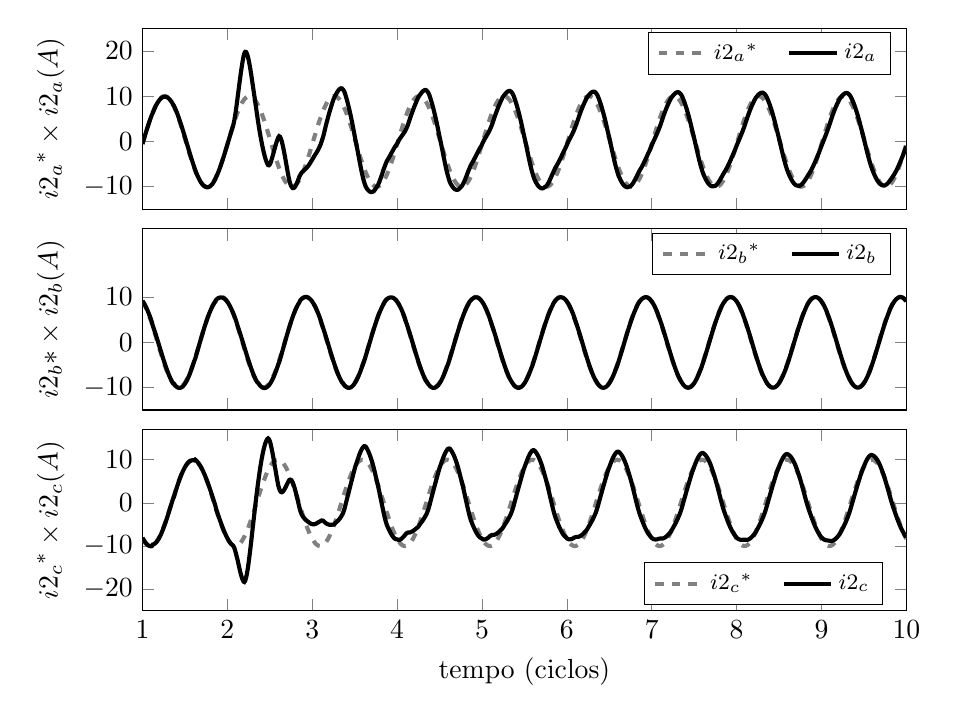
\begin{tikzpicture}

\begin{axis}[%
width=0.8\textwidth,
height=0.189701500343624\textwidth,
scale only axis,
xmin=0.0166666666666667,
xmax=0.166666666666667,
xtick={0.0166666666666667,0.0333333333333333,0.05,0.0666666666666667,0.0833333333333333,0.1,0.116666666666667,0.133333333333333,0.15,0.166666666666667},
xticklabels={\empty},
ymin=-15,
ymax=25,
ytick={-10,   0,  10},
ylabel={${\text{i2}_\text{b}}\text{* }\times\text{ i2}_\text{b}\text{ (A)}$},
name=plot2,
legend style={draw=black,fill=white,legend cell align=left},
scaled x ticks = false,
legend columns=-1,
legend style={/tikz/every even column/.append style={column sep=0.3cm}},
legend style={font=\footnotesize}
]
\addplot [color=gray,dashed,line width=1.5pt]
  table[row sep=crcr]{0.0166583333333333	8.95711760239421\\
0.016825	8.66025403784447\\
0.0169916666666667	8.32921240710107\\
0.0171583333333333	7.96529918024204\\
0.017325	7.56995055651764\\
0.0174916666666667	7.1447267963281\\
0.0176583333333333	6.69130606358865\\
0.017825	6.21147780278317\\
0.0179916666666667	5.70713567684438\\
0.0181583333333333	5.18027009373136\\
0.018325	4.63296035119867\\
0.0184916666666667	4.06736643075805\\
0.0186583333333333	3.4857204732182\\
0.018825	2.89031796944476\\
0.0189916666666667	2.28350870110659\\
0.0191583333333333	1.66768746716105\\
0.019325	1.04528463267656\\
0.0194916666666667	0.418756537292012\\
0.0196583333333333	-0.20942419883356\\
0.019825	-0.836778433323152\\
0.0199916666666667	-1.46083028562412\\
0.0201583333333333	-2.0791169081776\\
0.020325	-2.68919820615267\\
0.0204916666666667	-3.28866646738586\\
0.0206583333333333	-3.87515586452106\\
0.020825	-4.44635179184931\\
0.0209916666666667	-5.00000000000005\\
0.0211583333333333	-5.53391549243349\\
0.021325	-6.0459911486238\\
0.0214916666666667	-6.53420603990112\\
0.0216583333333333	-6.99663340513372\\
0.021825	-7.43144825477402\\
0.0219916666666667	-7.83693457325848\\
0.0221583333333333	-8.21149209133713\\
0.022325	-8.55364260160516\\
0.0224916666666667	-8.86203579231225\\
0.0226583333333333	-9.13545457642611\\
0.022825	-9.37281989491902\\
0.0229916666666667	-9.57319497532079\\
0.0231583333333333	-9.73578902873172\\
0.023325	-9.85996037070517\\
0.0234916666666667	-9.94521895368285\\
0.0236583333333333	-9.99122830098871\\
0.023825	-9.99780683474858\\
0.0239916666666667	-9.96492859249517\\
0.0241583333333333	-9.89272332963001\\
0.024325	-9.78147600733818\\
0.0244916666666667	-9.63162566797671\\
0.0246583333333333	-9.44376370237494\\
0.024825	-9.21863151588513\\
0.0249916666666667	-8.95711760239425\\
0.0251583333333333	-8.66025403784451\\
0.025325	-8.32921240710111\\
0.0254916666666667	-7.96529918024207\\
0.0256583333333333	-7.56995055651767\\
0.025825	-7.14472679632814\\
0.0259916666666667	-6.69130606358868\\
0.0261583333333333	-6.2114778027832\\
0.026325	-5.70713567684441\\
0.0264916666666667	-5.18027009373139\\
0.0266583333333333	-4.6329603511987\\
0.026825	-4.06736643075807\\
0.0269916666666667	-3.48572047321821\\
0.0271583333333333	-2.89031796944477\\
0.027325	-2.28350870110661\\
0.0274916666666667	-1.66768746716106\\
0.0276583333333333	-1.04528463267656\\
0.027825	-0.418756537292015\\
0.0279916666666667	0.209424198833559\\
0.0281583333333333	0.836778433323154\\
0.028325	1.46083028562412\\
0.0284916666666667	2.07911690817761\\
0.0286583333333333	2.68919820615268\\
0.028825	3.28866646738587\\
0.0289916666666667	3.87515586452107\\
0.0291583333333333	4.44635179184933\\
0.029325	5.00000000000006\\
0.0294916666666667	5.53391549243351\\
0.0296583333333333	6.04599114862383\\
0.029825	6.53420603990114\\
0.0299916666666667	6.99663340513375\\
0.0301583333333333	7.43144825477405\\
0.030325	7.83693457325851\\
0.0304916666666667	8.21149209133716\\
0.0306583333333333	8.55364260160519\\
0.030825	8.86203579231228\\
0.0309916666666667	9.13545457642615\\
0.0311583333333333	9.37281989491906\\
0.031325	9.57319497532082\\
0.0314916666666667	9.73578902873176\\
0.0316583333333333	9.85996037070521\\
0.031825	9.94521895368289\\
0.0319916666666667	9.99122830098875\\
0.0321583333333333	9.99780683474862\\
0.032325	9.96492859249521\\
0.0324916666666667	9.89272332963005\\
0.0326583333333333	9.78147600733822\\
0.032825	9.63162566797675\\
0.0329916666666667	9.44376370237498\\
0.0331583333333333	9.21863151588517\\
0.033325	8.95711760239429\\
0.0334916666666667	8.66025403784455\\
0.0336583333333333	8.32921240710115\\
0.033825	7.96529918024211\\
0.0339916666666667	7.56995055651771\\
0.0341583333333333	7.14472679632817\\
0.034325	6.69130606358871\\
0.0344916666666667	6.21147780278323\\
0.0346583333333333	5.70713567684443\\
0.034825	5.18027009373141\\
0.0349916666666667	4.63296035119872\\
0.0351583333333333	4.06736643075809\\
0.035325	3.48572047321823\\
0.0354916666666667	2.89031796944478\\
0.0356583333333333	2.28350870110662\\
0.035825	1.66768746716107\\
0.0359916666666667	1.04528463267657\\
0.0361583333333333	0.418756537292022\\
0.036325	-0.209424198833557\\
0.0364916666666667	-0.836778433323154\\
0.0366583333333333	-1.46083028562413\\
0.036825	-2.07911690817762\\
0.0369916666666667	-2.68919820615269\\
0.0371583333333333	-3.28866646738588\\
0.037325	-3.87515586452109\\
0.0374916666666667	-4.44635179184934\\
0.0376583333333333	-5.00000000000008\\
0.037825	-5.53391549243353\\
0.0379916666666667	-6.04599114862385\\
0.0381583333333333	-6.53420603990117\\
0.038325	-6.99663340513378\\
0.0384916666666667	-7.43144825477408\\
0.0386583333333333	-7.83693457325854\\
0.038825	-8.21149209133719\\
0.0389916666666667	-8.55364260160523\\
0.0391583333333333	-8.86203579231232\\
0.039325	-9.13545457642618\\
0.0394916666666667	-9.3728198949191\\
0.0396583333333333	-9.57319497532086\\
0.039825	-9.7357890287318\\
0.0399916666666667	-9.85996037070525\\
0.0401583333333333	-9.94521895368294\\
0.040325	-9.99122830098879\\
0.0404916666666667	-9.99780683474866\\
0.0406583333333333	-9.96492859249525\\
0.040825	-9.89272332963009\\
0.0409916666666667	-9.78147600733827\\
0.0411583333333333	-9.63162566797679\\
0.041325	-9.44376370237502\\
0.0414916666666667	-9.21863151588521\\
0.0416583333333333	-8.95711760239433\\
0.041825	-8.66025403784458\\
0.0419916666666667	-8.32921240710118\\
0.0421583333333333	-7.96529918024214\\
0.042325	-7.56995055651774\\
0.0424916666666667	-7.1447267963282\\
0.0426583333333333	-6.69130606358874\\
0.042825	-6.21147780278325\\
0.0429916666666667	-5.70713567684446\\
0.0431583333333333	-5.18027009373143\\
0.043325	-4.63296035119874\\
0.0434916666666667	-4.06736643075811\\
0.0436583333333333	-3.48572047321825\\
0.043825	-2.8903179694448\\
0.0439916666666667	-2.28350870110663\\
0.0441583333333333	-1.66768746716108\\
0.044325	-1.04528463267658\\
0.0444916666666667	-0.418756537292025\\
0.0446583333333333	0.209424198833555\\
0.044825	0.836778433323156\\
0.0449916666666667	1.46083028562413\\
0.0451583333333333	2.07911690817762\\
0.045325	2.6891982061527\\
0.0454916666666667	3.28866646738589\\
0.0456583333333333	3.8751558645211\\
0.045825	4.44635179184936\\
0.0459916666666667	5.0000000000001\\
0.0461583333333333	5.53391549243356\\
0.046325	6.04599114862388\\
0.0464916666666667	6.5342060399012\\
0.0466583333333333	6.99663340513381\\
0.046825	7.43144825477411\\
0.0469916666666667	7.83693457325858\\
0.0471583333333333	8.21149209133723\\
0.047325	8.55364260160527\\
0.0474916666666667	8.86203579231236\\
0.0476583333333333	9.13545457642623\\
0.047825	9.37281989491914\\
0.0479916666666667	9.57319497532091\\
0.0481583333333333	9.73578902873184\\
0.048325	9.85996037070529\\
0.0484916666666667	9.94521895368298\\
0.0486583333333333	9.99122830098883\\
0.048825	9.99780683474871\\
0.0489916666666667	9.9649285924953\\
0.0491583333333333	9.89272332963014\\
0.049325	9.78147600733831\\
0.0494916666666667	9.63162566797684\\
0.0496583333333333	9.44376370237506\\
0.049825	9.21863151588525\\
0.0499916666666667	8.95711760239437\\
0.0501583333333333	8.66025403784462\\
0.050325	8.32921240710123\\
0.0504916666666667	7.96529918024218\\
0.0506583333333333	7.56995055651778\\
0.050825	7.14472679632824\\
0.0509916666666667	6.69130606358878\\
0.0511583333333333	6.21147780278329\\
0.051325	5.70713567684449\\
0.0514916666666667	5.18027009373146\\
0.0516583333333333	4.63296035119876\\
0.051825	4.06736643075813\\
0.0519916666666667	3.48572047321827\\
0.0521583333333333	2.89031796944481\\
0.052325	2.28350870110664\\
0.0524916666666667	1.66768746716109\\
0.0526583333333333	1.04528463267659\\
0.052825	0.418756537292029\\
0.0529916666666667	-0.209424198833554\\
0.0531583333333333	-0.836778433323157\\
0.053325	-1.46083028562414\\
0.0534916666666667	-2.07911690817763\\
0.0536583333333333	-2.68919820615271\\
0.053825	-3.2886664673859\\
0.0539916666666667	-3.87515586452112\\
0.0541583333333333	-4.44635179184938\\
0.054325	-5.00000000000012\\
0.0544916666666667	-5.53391549243358\\
0.0546583333333333	-6.0459911486239\\
0.054825	-6.53420603990122\\
0.0549916666666667	-6.99663340513384\\
0.0551583333333333	-7.43144825477414\\
0.055325	-7.83693457325861\\
0.0554916666666667	-8.21149209133726\\
0.0556583333333333	-8.5536426016053\\
0.055825	-8.86203579231239\\
0.0559916666666667	-9.13545457642627\\
0.0561583333333333	-9.37281989491918\\
0.056325	-9.57319497532095\\
0.0564916666666667	-9.73578902873188\\
0.0566583333333333	-9.85996037070534\\
0.056825	-9.94521895368302\\
0.0569916666666667	-9.99122830098888\\
0.0571583333333333	-9.99780683474875\\
0.057325	-9.96492859249534\\
0.0574916666666667	-9.89272332963018\\
0.0576583333333333	-9.78147600733836\\
0.057825	-9.63162566797688\\
0.0579916666666667	-9.44376370237511\\
0.0581583333333333	-9.21863151588529\\
0.058325	-8.95711760239441\\
0.0584916666666667	-8.66025403784466\\
0.0586583333333333	-8.32921240710126\\
0.058825	-7.96529918024222\\
0.0589916666666667	-7.56995055651781\\
0.0591583333333333	-7.14472679632827\\
0.059325	-6.69130606358881\\
0.0594916666666667	-6.21147780278331\\
0.0596583333333333	-5.70713567684451\\
0.059825	-5.18027009373148\\
0.0599916666666667	-4.63296035119878\\
0.0601583333333333	-4.06736643075815\\
0.060325	-3.48572047321828\\
0.0604916666666667	-2.89031796944483\\
0.0606583333333333	-2.28350870110665\\
0.060825	-1.6676874671611\\
0.0609916666666667	-1.04528463267659\\
0.0611583333333333	-0.418756537292034\\
0.061325	0.209424198833552\\
0.0614916666666667	0.836778433323157\\
0.0616583333333333	1.46083028562414\\
0.061825	2.07911690817764\\
0.0619916666666667	2.68919820615272\\
0.0621583333333333	3.28866646738591\\
0.062325	3.87515586452113\\
0.0624916666666667	4.4463517918494\\
0.0626583333333333	5.00000000000014\\
0.062825	5.5339154924336\\
0.0629916666666667	6.04599114862392\\
0.0631583333333333	6.53420603990125\\
0.063325	6.99663340513387\\
0.0634916666666667	7.43144825477417\\
0.0636583333333333	7.83693457325864\\
0.063825	8.2114920913373\\
0.0639916666666667	8.55364260160534\\
0.0641583333333333	8.86203579231243\\
0.064325	9.1354545764263\\
0.0644916666666667	9.37281989491922\\
0.0646583333333333	9.57319497532098\\
0.064825	9.73578902873192\\
0.0649916666666667	9.85996037070537\\
0.0651583333333333	9.94521895368306\\
0.065325	9.99122830098892\\
0.0654916666666667	9.99780683474879\\
0.0656583333333333	9.96492859249538\\
0.065825	9.89272332963022\\
0.0659916666666667	9.78147600733839\\
0.0661583333333333	9.63162566797691\\
0.066325	9.44376370237514\\
0.0664916666666667	9.21863151588533\\
0.0666583333333333	8.95711760239444\\
0.066825	8.6602540378447\\
0.0669916666666667	8.3292124071013\\
0.0671583333333333	7.96529918024225\\
0.067325	7.56995055651784\\
0.0674916666666667	7.1447267963283\\
0.0676583333333333	6.69130606358883\\
0.067825	6.21147780278334\\
0.0679916666666667	5.70713567684454\\
0.0681583333333333	5.1802700937315\\
0.068325	4.6329603511988\\
0.0684916666666667	4.06736643075817\\
0.0686583333333333	3.4857204732183\\
0.068825	2.89031796944484\\
0.0689916666666667	2.28350870110666\\
0.0691583333333333	1.6676874671611\\
0.069325	1.0452846326766\\
0.0694916666666667	0.418756537292036\\
0.0696583333333333	-0.209424198833552\\
0.069825	-0.836778433323159\\
0.0699916666666667	-1.46083028562414\\
0.0701583333333333	-2.07911690817764\\
0.070325	-2.68919820615273\\
0.0704916666666667	-3.28866646738592\\
0.0706583333333333	-3.87515586452114\\
0.070825	-4.44635179184941\\
0.0709916666666667	-5.00000000000016\\
0.0711583333333333	-5.53391549243362\\
0.071325	-6.04599114862394\\
0.0714916666666667	-6.53420603990127\\
0.0716583333333333	-6.99663340513388\\
0.071825	-7.43144825477419\\
0.0719916666666667	-7.83693457325866\\
0.0721583333333333	-8.21149209133732\\
0.072325	-8.55364260160536\\
0.0724916666666667	-8.86203579231245\\
0.0726583333333333	-9.13545457642633\\
0.072825	-9.37281989491924\\
0.0729916666666667	-9.57319497532101\\
0.0731583333333333	-9.73578902873195\\
0.073325	-9.8599603707054\\
0.0734916666666667	-9.94521895368309\\
0.0736583333333333	-9.99122830098895\\
0.073825	-9.99780683474882\\
0.0739916666666667	-9.96492859249541\\
0.0741583333333333	-9.89272332963025\\
0.074325	-9.78147600733842\\
0.0744916666666667	-9.63162566797694\\
0.0746583333333333	-9.44376370237517\\
0.074825	-9.21863151588536\\
0.0749916666666667	-8.95711760239447\\
0.0751583333333333	-8.66025403784472\\
0.075325	-8.32921240710132\\
0.0754916666666667	-7.96529918024228\\
0.0756583333333333	-7.56995055651787\\
0.075825	-7.14472679632832\\
0.0759916666666667	-6.69130606358885\\
0.0761583333333333	-6.21147780278336\\
0.076325	-5.70713567684455\\
0.0764916666666667	-5.18027009373152\\
0.0766583333333333	-4.63296035119882\\
0.076825	-4.06736643075818\\
0.0769916666666667	-3.48572047321831\\
0.0771583333333333	-2.89031796944486\\
0.077325	-2.28350870110667\\
0.0774916666666667	-1.66768746716112\\
0.0776583333333333	-1.04528463267661\\
0.077825	-0.418756537292044\\
0.0779916666666667	0.209424198833547\\
0.0781583333333333	0.836778433323155\\
0.078325	1.46083028562414\\
0.0784916666666667	2.07911690817764\\
0.0786583333333333	2.68919820615273\\
0.078825	3.28866646738593\\
0.0789916666666667	3.87515586452115\\
0.0791583333333333	4.44635179184942\\
0.079325	5.00000000000017\\
0.0794916666666667	5.53391549243363\\
0.0796583333333333	6.04599114862396\\
0.079825	6.53420603990128\\
0.0799916666666667	6.9966334051339\\
0.0801583333333333	7.43144825477421\\
0.080325	7.83693457325868\\
0.0804916666666667	8.21149209133734\\
0.0806583333333333	8.55364260160538\\
0.080825	8.86203579231248\\
0.0809916666666667	9.13545457642635\\
0.0811583333333333	9.37281989491927\\
0.081325	9.57319497532104\\
0.0814916666666667	9.73578902873198\\
0.0816583333333333	9.85996037070543\\
0.081825	9.94521895368312\\
0.0819916666666667	9.99122830098898\\
0.0821583333333333	9.99780683474885\\
0.082325	9.96492859249544\\
0.0824916666666667	9.89272332963028\\
0.0826583333333333	9.78147600733845\\
0.082825	9.63162566797698\\
0.0829916666666667	9.4437637023752\\
0.0831583333333333	9.21863151588539\\
0.083325	8.9571176023945\\
0.0834916666666667	8.66025403784476\\
0.0836583333333333	8.32921240710135\\
0.083825	7.96529918024231\\
0.0839916666666667	7.5699505565179\\
0.0841583333333333	7.14472679632835\\
0.084325	6.69130606358888\\
0.0844916666666667	6.21147780278338\\
0.0846583333333333	5.70713567684458\\
0.084825	5.18027009373154\\
0.0849916666666667	4.63296035119884\\
0.0851583333333333	4.0673664307582\\
0.085325	3.48572047321833\\
0.0854916666666667	2.89031796944487\\
0.0856583333333333	2.28350870110668\\
0.085825	1.66768746716112\\
0.0859916666666667	1.04528463267661\\
0.0861583333333333	0.418756537292048\\
0.086325	-0.209424198833544\\
0.0864916666666667	-0.836778433323155\\
0.0866583333333333	-1.46083028562414\\
0.086825	-2.07911690817765\\
0.0869916666666667	-2.68919820615273\\
0.0871583333333333	-3.28866646738594\\
0.087325	-3.87515586452116\\
0.0874916666666667	-4.44635179184943\\
0.0876583333333333	-5.00000000000018\\
0.087825	-5.53391549243365\\
0.0879916666666667	-6.04599114862398\\
0.0881583333333333	-6.5342060399013\\
0.088325	-6.99663340513393\\
0.0884916666666667	-7.43144825477423\\
0.0886583333333333	-7.83693457325871\\
0.088825	-8.21149209133737\\
0.0889916666666667	-8.55364260160541\\
0.0891583333333333	-8.86203579231251\\
0.089325	-9.13545457642639\\
0.0894916666666667	-9.37281989491931\\
0.0896583333333333	-9.57319497532107\\
0.089825	-9.73578902873201\\
0.0899916666666667	-9.85996037070547\\
0.0901583333333333	-9.94521895368316\\
0.090325	-9.99122830098902\\
0.0904916666666667	-9.99780683474889\\
0.0906583333333333	-9.96492859249548\\
0.090825	-9.89272332963032\\
0.0909916666666667	-9.78147600733849\\
0.0911583333333333	-9.63162566797701\\
0.091325	-9.44376370237524\\
0.0914916666666667	-9.21863151588543\\
0.0916583333333333	-8.95711760239454\\
0.091825	-8.66025403784479\\
0.0919916666666667	-8.32921240710138\\
0.0921583333333333	-7.96529918024234\\
0.092325	-7.56995055651792\\
0.0924916666666667	-7.14472679632838\\
0.0926583333333333	-6.69130606358891\\
0.092825	-6.21147780278341\\
0.0929916666666667	-5.7071356768446\\
0.0931583333333333	-5.18027009373156\\
0.093325	-4.63296035119886\\
0.0934916666666667	-4.06736643075822\\
0.0936583333333333	-3.48572047321834\\
0.093825	-2.89031796944488\\
0.0939916666666667	-2.2835087011067\\
0.0941583333333333	-1.66768746716113\\
0.094325	-1.04528463267662\\
0.0944916666666667	-0.418756537292053\\
0.0946583333333333	0.209424198833542\\
0.094825	0.836778433323155\\
0.0949916666666667	1.46083028562415\\
0.0951583333333333	2.07911690817765\\
0.095325	2.68919820615274\\
0.0954916666666667	3.28866646738595\\
0.0956583333333333	3.87515586452117\\
0.095825	4.44635179184944\\
0.0959916666666667	5.0000000000002\\
0.0961583333333333	5.53391549243367\\
0.096325	6.045991148624\\
0.0964916666666667	6.53420603990133\\
0.0966583333333333	6.99663340513395\\
0.096825	7.43144825477426\\
0.0969916666666667	7.83693457325874\\
0.0971583333333333	8.2114920913374\\
0.097325	8.55364260160545\\
0.0974916666666667	8.86203579231255\\
0.0976583333333333	9.13545457642642\\
0.097825	9.37281989491934\\
0.0979916666666667	9.57319497532111\\
0.0981583333333333	9.73578902873205\\
0.098325	9.85996037070551\\
0.0984916666666667	9.9452189536832\\
0.0986583333333333	9.99122830098905\\
0.098825	9.99780683474893\\
0.0989916666666667	9.96492859249552\\
0.0991583333333333	9.89272332963036\\
0.099325	9.78147600733853\\
0.0994916666666667	9.63162566797705\\
0.0996583333333333	9.44376370237527\\
0.099825	9.21863151588546\\
0.0999916666666667	8.95711760239457\\
0.100158333333333	8.66025403784482\\
0.100325	8.32921240710142\\
0.100491666666667	7.96529918024237\\
0.100658333333333	7.56995055651795\\
0.100825	7.1447267963284\\
0.100991666666667	6.69130606358893\\
0.101158333333333	6.21147780278343\\
0.101325	5.70713567684462\\
0.101491666666667	5.18027009373158\\
0.101658333333333	4.63296035119887\\
0.101825	4.06736643075823\\
0.101991666666667	3.48572047321836\\
0.102158333333333	2.89031796944489\\
0.102325	2.2835087011067\\
0.102491666666667	1.66768746716114\\
0.102658333333333	1.04528463267662\\
0.102825	0.418756537292053\\
0.102991666666667	-0.209424198833544\\
0.103158333333333	-0.83677843332316\\
0.103325	-1.46083028562415\\
0.103491666666667	-2.07911690817766\\
0.103658333333333	-2.68919820615275\\
0.103825	-3.28866646738596\\
0.103991666666667	-3.87515586452119\\
0.104158333333333	-4.44635179184946\\
0.104325	-5.00000000000022\\
0.104491666666667	-5.53391549243368\\
0.104658333333333	-6.04599114862402\\
0.104825	-6.53420603990135\\
0.104991666666667	-6.99663340513398\\
0.105158333333333	-7.43144825477429\\
0.105325	-7.83693457325877\\
0.105491666666667	-8.21149209133743\\
0.105658333333333	-8.55364260160548\\
0.105825	-8.86203579231258\\
0.105991666666667	-9.13545457642645\\
0.106158333333333	-9.37281989491938\\
0.106325	-9.57319497532115\\
0.106491666666667	-9.73578902873209\\
0.106658333333333	-9.85996037070554\\
0.106825	-9.94521895368323\\
0.106991666666667	-9.99122830098909\\
0.107158333333333	-9.99780683474897\\
0.107325	-9.96492859249556\\
0.107491666666667	-9.8927233296304\\
0.107658333333333	-9.78147600733856\\
0.107825	-9.63162566797709\\
0.107991666666667	-9.44376370237531\\
0.108158333333333	-9.21863151588549\\
0.108325	-8.95711760239461\\
0.108491666666667	-8.66025403784485\\
0.108658333333333	-8.32921240710145\\
0.108825	-7.9652991802424\\
0.108991666666667	-7.56995055651798\\
0.109158333333333	-7.14472679632843\\
0.109325	-6.69130606358896\\
0.109491666666667	-6.21147780278346\\
0.109658333333333	-5.70713567684465\\
0.109825	-5.18027009373161\\
0.109991666666667	-4.6329603511989\\
0.110158333333333	-4.06736643075825\\
0.110325	-3.48572047321838\\
0.110491666666667	-2.89031796944491\\
0.110658333333333	-2.28350870110672\\
0.110825	-1.66768746716115\\
0.110991666666667	-1.04528463267663\\
0.111158333333333	-0.418756537292063\\
0.111325	0.209424198833538\\
0.111491666666667	0.836778433323156\\
0.111658333333333	1.46083028562415\\
0.111825	2.07911690817766\\
0.111991666666667	2.68919820615276\\
0.112158333333333	3.28866646738597\\
0.112325	3.8751558645212\\
0.112491666666667	4.44635179184947\\
0.112658333333333	5.00000000000023\\
0.112825	5.5339154924337\\
0.112991666666667	6.04599114862404\\
0.113158333333333	6.53420603990138\\
0.113325	6.996633405134\\
0.113491666666667	7.43144825477432\\
0.113658333333333	7.8369345732588\\
0.113825	8.21149209133746\\
0.113991666666667	8.55364260160551\\
0.114158333333333	8.86203579231261\\
0.114325	9.13545457642649\\
0.114491666666667	9.37281989491941\\
0.114658333333333	9.57319497532118\\
0.114825	9.73578902873213\\
0.114991666666667	9.85996037070558\\
0.115158333333333	9.94521895368328\\
0.115325	9.99122830098913\\
0.115491666666667	9.99780683474901\\
0.115658333333333	9.9649285924956\\
0.115825	9.89272332963044\\
0.115991666666667	9.78147600733861\\
0.116158333333333	9.63162566797713\\
0.116325	9.44376370237535\\
0.116491666666667	9.21863151588554\\
0.116658333333333	8.95711760239465\\
0.116825	8.66025403784489\\
0.116991666666667	8.32921240710149\\
0.117158333333333	7.96529918024244\\
0.117325	7.56995055651802\\
0.117491666666667	7.14472679632847\\
0.117658333333333	6.69130606358899\\
0.117825	6.21147780278349\\
0.117991666666667	5.70713567684468\\
0.118158333333333	5.18027009373164\\
0.118325	4.63296035119892\\
0.118491666666667	4.06736643075828\\
0.118658333333333	3.48572047321839\\
0.118825	2.89031796944493\\
0.118991666666667	2.28350870110673\\
0.119158333333333	1.66768746716117\\
0.119325	1.04528463267664\\
0.119491666666667	0.418756537292069\\
0.119658333333333	-0.209424198833534\\
0.119825	-0.836778433323155\\
0.119991666666667	-1.46083028562415\\
0.120158333333333	-2.07911690817766\\
0.120325	-2.68919820615276\\
0.120491666666667	-3.28866646738597\\
0.120658333333333	-3.87515586452121\\
0.120825	-4.44635179184949\\
0.120991666666667	-5.00000000000025\\
0.121158333333333	-5.53391549243372\\
0.121325	-6.04599114862406\\
0.121491666666667	-6.53420603990139\\
0.121658333333333	-6.99663340513402\\
0.121825	-7.43144825477434\\
0.121991666666667	-7.83693457325882\\
0.122158333333333	-8.21149209133749\\
0.122325	-8.55364260160554\\
0.122491666666667	-8.86203579231264\\
0.122658333333333	-9.13545457642652\\
0.122825	-9.37281989491945\\
0.122991666666667	-9.57319497532122\\
0.123158333333333	-9.73578902873216\\
0.123325	-9.85996037070562\\
0.123491666666667	-9.94521895368331\\
0.123658333333333	-9.99122830098917\\
0.123825	-9.99780683474905\\
0.123991666666667	-9.96492859249564\\
0.124158333333333	-9.89272332963048\\
0.124325	-9.78147600733865\\
0.124491666666667	-9.63162566797717\\
0.124658333333333	-9.44376370237539\\
0.124825	-9.21863151588557\\
0.124991666666667	-8.95711760239469\\
0.125158333333333	-8.66025403784493\\
0.125325	-8.32921240710152\\
0.125491666666667	-7.96529918024247\\
0.125658333333333	-7.56995055651805\\
0.125825	-7.1447267963285\\
0.125991666666667	-6.69130606358902\\
0.126158333333333	-6.21147780278352\\
0.126325	-5.7071356768447\\
0.126491666666667	-5.18027009373166\\
0.126658333333333	-4.63296035119894\\
0.126825	-4.0673664307583\\
0.126991666666667	-3.48572047321841\\
0.127158333333333	-2.89031796944494\\
0.127325	-2.28350870110675\\
0.127491666666667	-1.66768746716117\\
0.127658333333333	-1.04528463267665\\
0.127825	-0.418756537292072\\
0.127991666666667	0.209424198833532\\
0.128158333333333	0.836778433323155\\
0.128325	1.46083028562416\\
0.128491666666667	2.07911690817767\\
0.128658333333333	2.68919820615277\\
0.128825	3.28866646738599\\
0.128991666666667	3.87515586452122\\
0.129158333333333	4.4463517918495\\
0.129325	5.00000000000027\\
0.129491666666667	5.53391549243374\\
0.129658333333333	6.04599114862408\\
0.129825	6.53420603990142\\
0.129991666666667	6.99663340513405\\
0.130158333333333	7.43144825477437\\
0.130325	7.83693457325885\\
0.130491666666667	8.21149209133752\\
0.130658333333333	8.55364260160558\\
0.130825	8.86203579231268\\
0.130991666666667	9.13545457642656\\
0.131158333333333	9.37281989491949\\
0.131325	9.57319497532126\\
0.131491666666667	9.7357890287322\\
0.131658333333333	9.85996037070566\\
0.131825	9.94521895368336\\
0.131991666666667	9.99122830098921\\
0.132158333333333	9.99780683474909\\
0.132325	9.96492859249568\\
0.132491666666667	9.89272332963052\\
0.132658333333333	9.78147600733869\\
0.132825	9.63162566797721\\
0.132991666666667	9.44376370237543\\
0.133158333333333	9.21863151588561\\
0.133325	8.95711760239472\\
0.133491666666667	8.66025403784496\\
0.133658333333333	8.32921240710155\\
0.133825	7.9652991802425\\
0.133991666666667	7.56995055651808\\
0.134158333333333	7.14472679632853\\
0.134325	6.69130606358905\\
0.134491666666667	6.21147780278354\\
0.134658333333333	5.70713567684473\\
0.134825	5.18027009373168\\
0.134991666666667	4.63296035119896\\
0.135158333333333	4.06736643075831\\
0.135325	3.48572047321843\\
0.135491666666667	2.89031796944495\\
0.135658333333333	2.28350870110675\\
0.135825	1.66768746716118\\
0.135991666666667	1.04528463267665\\
0.136158333333333	0.418756537292075\\
0.136325	-0.209424198833533\\
0.136491666666667	-0.83677843332316\\
0.136658333333333	-1.46083028562416\\
0.136825	-2.07911690817768\\
0.136991666666667	-2.68919820615279\\
0.137158333333333	-3.288666467386\\
0.137325	-3.87515586452124\\
0.137491666666667	-4.44635179184952\\
0.137658333333333	-5.00000000000029\\
0.137825	-5.53391549243377\\
0.137991666666667	-6.04599114862411\\
0.138158333333333	-6.53420603990145\\
0.138325	-6.99663340513408\\
0.138491666666667	-7.4314482547744\\
0.138658333333333	-7.83693457325889\\
0.138825	-8.21149209133756\\
0.138991666666667	-8.55364260160561\\
0.139158333333333	-8.86203579231272\\
0.139325	-9.1354545764266\\
0.139491666666667	-9.37281989491953\\
0.139658333333333	-9.5731949753213\\
0.139825	-9.73578902873225\\
0.139991666666667	-9.8599603707057\\
0.140158333333333	-9.9452189536834\\
0.140325	-9.99122830098926\\
0.140491666666667	-9.99780683474913\\
0.140658333333333	-9.96492859249572\\
0.140825	-9.89272332963056\\
0.140991666666667	-9.78147600733873\\
0.141158333333333	-9.63162566797725\\
0.141325	-9.44376370237547\\
0.141491666666667	-9.21863151588565\\
0.141658333333333	-8.95711760239476\\
0.141825	-8.660254037845\\
0.141991666666667	-8.32921240710159\\
0.142158333333333	-7.96529918024254\\
0.142325	-7.56995055651812\\
0.142491666666667	-7.14472679632856\\
0.142658333333333	-6.69130606358908\\
0.142825	-6.21147780278357\\
0.142991666666667	-5.70713567684475\\
0.143158333333333	-5.18027009373171\\
0.143325	-4.63296035119899\\
0.143491666666667	-4.06736643075833\\
0.143658333333333	-3.48572047321844\\
0.143825	-2.89031796944497\\
0.143991666666667	-2.28350870110677\\
0.144158333333333	-1.66768746716119\\
0.144325	-1.04528463267666\\
0.144491666666667	-0.41875653729208\\
0.144658333333333	0.20942419883353\\
0.144825	0.836778433323158\\
0.144991666666667	1.46083028562416\\
0.145158333333333	2.07911690817769\\
0.145325	2.68919820615279\\
0.145491666666667	3.28866646738601\\
0.145658333333333	3.87515586452125\\
0.145825	4.44635179184954\\
0.145991666666667	5.0000000000003\\
0.146158333333333	5.53391549243378\\
0.146325	6.04599114862413\\
0.146491666666667	6.53420603990147\\
0.146658333333333	6.99663340513411\\
0.146825	7.43144825477443\\
0.146991666666667	7.83693457325891\\
0.147158333333333	8.21149209133759\\
0.147325	8.55364260160564\\
0.147491666666667	8.86203579231275\\
0.147658333333333	9.13545457642663\\
0.147825	9.37281989491956\\
0.147991666666667	9.57319497532134\\
0.148158333333333	9.73578902873228\\
0.148325	9.85996037070574\\
0.148491666666667	9.94521895368344\\
0.148658333333333	9.9912283009893\\
0.148825	9.99780683474917\\
0.148991666666667	9.96492859249576\\
0.149158333333333	9.8927233296306\\
0.149325	9.78147600733877\\
0.149491666666667	9.63162566797729\\
0.149658333333333	9.44376370237551\\
0.149825	9.21863151588569\\
0.149991666666667	8.9571176023948\\
0.150158333333333	8.66025403784504\\
0.150325	8.32921240710163\\
0.150491666666667	7.96529918024257\\
0.150658333333333	7.56995055651815\\
0.150825	7.14472679632859\\
0.150991666666667	6.69130606358911\\
0.151158333333333	6.2114778027836\\
0.151325	5.70713567684478\\
0.151491666666667	5.18027009373173\\
0.151658333333333	4.63296035119901\\
0.151825	4.06736643075835\\
0.151991666666667	3.48572047321846\\
0.152158333333333	2.89031796944498\\
0.152325	2.28350870110678\\
0.152491666666667	1.6676874671612\\
0.152658333333333	1.04528463267667\\
0.152825	0.418756537292087\\
0.152991666666667	-0.209424198833525\\
0.153158333333333	-0.836778433323156\\
0.153325	-1.46083028562416\\
0.153491666666667	-2.07911690817769\\
0.153658333333333	-2.6891982061528\\
0.153825	-3.28866646738602\\
0.153991666666667	-3.87515586452126\\
0.154158333333333	-4.44635179184955\\
0.154325	-5.00000000000032\\
0.154491666666667	-5.5339154924338\\
0.154658333333333	-6.04599114862415\\
0.154825	-6.5342060399015\\
0.154991666666667	-6.99663340513413\\
0.155158333333333	-7.43144825477446\\
0.155325	-7.83693457325895\\
0.155491666666667	-8.21149209133762\\
0.155658333333333	-8.55364260160568\\
0.155825	-8.86203579231279\\
0.155991666666667	-9.13545457642667\\
0.156158333333333	-9.3728198949196\\
0.156325	-9.57319497532138\\
0.156491666666667	-9.73578902873233\\
0.156658333333333	-9.85996037070579\\
0.156825	-9.94521895368348\\
0.156991666666667	-9.99122830098934\\
0.157158333333333	-9.99780683474921\\
0.157325	-9.96492859249581\\
0.157491666666667	-9.89272332963065\\
0.157658333333333	-9.78147600733882\\
0.157825	-9.63162566797734\\
0.157991666666667	-9.44376370237556\\
0.158158333333333	-9.21863151588574\\
0.158325	-8.95711760239484\\
0.158491666666667	-8.66025403784508\\
0.158658333333333	-8.32921240710167\\
0.158825	-7.96529918024262\\
0.158991666666667	-7.56995055651819\\
0.159158333333333	-7.14472679632863\\
0.159325	-6.69130606358915\\
0.159491666666667	-6.21147780278364\\
0.159658333333333	-5.70713567684481\\
0.159825	-5.18027009373176\\
0.159991666666667	-4.63296035119904\\
0.160158333333333	-4.06736643075838\\
0.160325	-3.48572047321849\\
0.160491666666667	-2.890317969445\\
0.160658333333333	-2.2835087011068\\
0.160825	-1.66768746716122\\
0.160991666666667	-1.04528463267668\\
0.161158333333333	-0.418756537292097\\
0.161325	0.209424198833518\\
0.161491666666667	0.836778433323153\\
0.161658333333333	1.46083028562416\\
0.161825	2.07911690817769\\
0.161991666666667	2.6891982061528\\
0.162158333333333	3.28866646738603\\
0.162325	3.87515586452127\\
0.162491666666667	4.44635179184956\\
0.162658333333333	5.00000000000034\\
0.162825	5.53391549243382\\
0.162991666666667	6.04599114862417\\
0.163158333333333	6.53420603990152\\
0.163325	6.99663340513416\\
0.163491666666667	7.43144825477449\\
0.163658333333333	7.83693457325898\\
0.163825	8.21149209133765\\
0.163991666666667	8.55364260160571\\
0.164158333333333	8.86203579231282\\
0.164325	9.13545457642671\\
0.164491666666667	9.37281989491964\\
0.164658333333333	9.57319497532142\\
0.164825	9.73578902873236\\
0.164991666666667	9.85996037070582\\
0.165158333333333	9.94521895368352\\
0.165325	9.99122830098938\\
0.165491666666667	9.99780683474926\\
0.165658333333333	9.96492859249585\\
0.165825	9.89272332963069\\
0.165991666666667	9.78147600733886\\
0.166158333333333	9.63162566797738\\
0.166325	9.44376370237559\\
0.166491666666667	9.21863151588578\\
0.166658333333333	8.95711760239488\\
};
\addlegendentry{${\text{i2}_\text{b}}^\text{*}$};

\addplot [color=black,solid,line width=1.5pt]
  table[row sep=crcr]{0.0166583333333333	9.10238729436972\\
0.016825	8.81704993622876\\
0.0169916666666667	8.50071754137033\\
0.0171583333333333	8.15515004140646\\
0.017325	7.7819187867049\\
0.0174916666666667	7.38204974177135\\
0.0176583333333333	6.95626978050029\\
0.017825	6.50510560395105\\
0.0179916666666667	6.02945861112754\\
0.0181583333333333	5.53040314356191\\
0.018325	5.00924821301577\\
0.0184916666666667	4.46751489796481\\
0.0186583333333333	3.68981019134787\\
0.018825	3.14840956068264\\
0.0189916666666667	2.59416394011585\\
0.0191583333333333	2.02377684219615\\
0.019325	1.43881119869898\\
0.0194916666666667	0.841909769593364\\
0.0196583333333333	0.235780957939821\\
0.019825	-0.376689340170496\\
0.0199916666666667	-0.992665526242936\\
0.0201583333333333	-1.60920663242736\\
0.020325	-2.22329353670832\\
0.0204916666666667	-2.83190601073707\\
0.0206583333333333	-3.43206068203698\\
0.020825	-4.02042104637285\\
0.0209916666666667	-4.59498130928033\\
0.0211583333333333	-5.15341682461041\\
0.021325	-5.6940962192604\\
0.0214916666666667	-6.21505582977236\\
0.0216583333333333	-6.71378044678016\\
0.021825	-7.18751402421548\\
0.0219916666666667	-7.6333168162301\\
0.0221583333333333	-8.04867680302019\\
0.022325	-8.43126236325755\\
0.0224916666666667	-8.77900373523377\\
0.0226583333333333	-9.09008498121201\\
0.022825	-9.15855337492306\\
0.0229916666666667	-9.42861378862864\\
0.0231583333333333	-9.65793002398938\\
0.023325	-9.84203175689098\\
0.0234916666666667	-9.97985634821345\\
0.0236583333333333	-10.0713474398235\\
0.023825	-10.1165549780692\\
0.0239916666666667	-10.1159383416511\\
0.0241583333333333	-10.0698886487835\\
0.024325	-9.97914771255928\\
0.0244916666666667	-9.84467529451614\\
0.0246583333333333	-9.66760532286042\\
0.024825	-9.44931901487656\\
0.0249916666666667	-9.19133428032041\\
0.0251583333333333	-8.8945965624705\\
0.025325	-8.56015786213606\\
0.0254916666666667	-8.18882959610245\\
0.0256583333333333	-7.78203825639882\\
0.025825	-7.34193745850652\\
0.0259916666666667	-6.871066065311\\
0.0261583333333333	-6.37234524011466\\
0.026325	-5.84845377190004\\
0.0264916666666667	-5.30212355465025\\
0.0266583333333333	-4.73605099633701\\
0.026825	-4.15290088980286\\
0.0269916666666667	-3.7463128418275\\
0.0271583333333333	-3.10098116111065\\
0.027325	-2.44739188124668\\
0.0274916666666667	-1.79053931585367\\
0.0276583333333333	-1.13327765870239\\
0.027825	-0.477924319106184\\
0.0279916666666667	0.173209663659246\\
0.0281583333333333	0.81818389481377\\
0.028325	1.45483512926401\\
0.0284916666666667	2.08120905361234\\
0.0286583333333333	2.69541683114933\\
0.028825	3.29561201161392\\
0.0289916666666667	3.88022294753529\\
0.0291583333333333	4.44714029176902\\
0.029325	4.99439015782883\\
0.0294916666666667	5.51947855033307\\
0.0296583333333333	6.01988736030132\\
0.029825	6.49370710499595\\
0.0299916666666667	6.93963550745553\\
0.0301583333333333	7.3567961627066\\
0.030325	7.74446827210866\\
0.0304916666666667	8.10180024444722\\
0.0306583333333333	8.42799192122998\\
0.030825	8.72224797849278\\
0.0309916666666667	8.98379451656429\\
0.0311583333333333	9.39000247520132\\
0.031325	9.54893851207278\\
0.0314916666666667	9.67501312493445\\
0.0316583333333333	9.76956673991744\\
0.031825	9.83213375604548\\
0.0319916666666667	9.86203092932595\\
0.0321583333333333	9.85882018895445\\
0.032325	9.82186948854932\\
0.0324916666666667	9.7509584363675\\
0.0326583333333333	9.64582294926668\\
0.032825	9.50631560990461\\
0.0329916666666667	9.33243620129852\\
0.0331583333333333	9.12407992641987\\
0.033325	8.88199693232614\\
0.0334916666666667	8.60690761693528\\
0.0336583333333333	8.30031817371014\\
0.033825	7.96381783130639\\
0.0339916666666667	7.59858035831388\\
0.0341583333333333	7.20550175883682\\
0.034325	6.78510676631586\\
0.0344916666666667	6.33834029028864\\
0.0346583333333333	5.8662884047453\\
0.034825	5.37023786238818\\
0.0349916666666667	4.85163190263994\\
0.0351583333333333	4.28149658577571\\
0.035325	3.58762676973298\\
0.0354916666666667	3.0456994482591\\
0.0356583333333333	2.4865038492782\\
0.035825	1.91102787172691\\
0.0359916666666667	1.32189078050082\\
0.0361583333333333	0.721938962011906\\
0.036325	0.113855158360438\\
0.0364916666666667	-0.499365898498088\\
0.0366583333333333	-1.11503128292631\\
0.036825	-1.73025520539475\\
0.0369916666666667	-2.34208378847066\\
0.0371583333333333	-2.94748587657552\\
0.037325	-3.5431400706758\\
0.0374916666666667	-4.1265231476695\\
0.0376583333333333	-4.69508199372783\\
0.037825	-5.24699481009654\\
0.0379916666666667	-5.78041375264997\\
0.0381583333333333	-6.29307974931665\\
0.038325	-6.78253811247046\\
0.0384916666666667	-7.24596610272513\\
0.0386583333333333	-7.6810872056987\\
0.038825	-8.08574080491781\\
0.0389916666666667	-8.45801037504019\\
0.0391583333333333	-8.79620068499962\\
0.039325	-8.96806487507886\\
0.0394916666666667	-9.21070528346815\\
0.0396583333333333	-9.47108643131567\\
0.039825	-9.69006577542452\\
0.0399916666666667	-9.86604802286814\\
0.0401583333333333	-9.99862843742934\\
0.040325	-10.0876819809747\\
0.0404916666666667	-10.1331917117651\\
0.0406583333333333	-10.1355416577069\\
0.040825	-10.0949836782007\\
0.0409916666666667	-10.0120127334088\\
0.0411583333333333	-9.88722687874503\\
0.041325	-9.72133156733559\\
0.0414916666666667	-9.51541879850157\\
0.0416583333333333	-9.26995328123422\\
0.041825	-8.98572454913961\\
0.0419916666666667	-8.66322314753683\\
0.0421583333333333	-8.30335136347556\\
0.042325	-7.90765316365763\\
0.0424916666666667	-7.47802658774969\\
0.0426583333333333	-7.0169137009076\\
0.042825	-6.52642947709798\\
0.0429916666666667	-6.00887733160312\\
0.0431583333333333	-5.46662604543119\\
0.043325	-4.90211625430936\\
0.0434916666666667	-4.48494333559065\\
0.0436583333333333	-3.8590351634337\\
0.043825	-3.2118487319502\\
0.0439916666666667	-2.5557754004136\\
0.0441583333333333	-1.89397286683257\\
0.044325	-1.22893143241073\\
0.0444916666666667	-0.563306382147479\\
0.0446583333333333	0.100389856630612\\
0.044825	0.759488778059827\\
0.0449916666666667	1.41140264559457\\
0.0451583333333333	2.05372800650602\\
0.045325	2.68418786236869\\
0.0454916666666667	3.3006105803122\\
0.0456583333333333	3.90115164165044\\
0.045825	4.48323533437549\\
0.0459916666666667	5.04441328155281\\
0.0461583333333333	5.5818940948016\\
0.046325	6.0933288931626\\
0.0464916666666667	6.57703266031942\\
0.0466583333333333	7.03168592527747\\
0.046825	7.45653884038628\\
0.0469916666666667	7.85052919185026\\
0.0471583333333333	8.21278991052803\\
0.047325	8.54250647974175\\
0.0474916666666667	8.83892137915094\\
0.0476583333333333	9.26324073490593\\
0.047825	9.46108564493796\\
0.0479916666666667	9.62395420189803\\
0.0481583333333333	9.75447445593996\\
0.048325	9.85256615795213\\
0.0484916666666667	9.91760332315369\\
0.0486583333333333	9.94912495301349\\
0.048825	9.94634598884029\\
0.0489916666666667	9.90895228811722\\
0.0491583333333333	9.83654546284874\\
0.049325	9.72882165016644\\
0.0494916666666667	9.58562670339993\\
0.0496583333333333	9.40692140087188\\
0.049825	9.19280839746856\\
0.0499916666666667	8.94410631419182\\
0.0501583333333333	8.66194019234958\\
0.050325	8.34784961980865\\
0.0504916666666667	8.00313239038802\\
0.0506583333333333	7.62874612085978\\
0.050825	7.22560396909269\\
0.0509916666666667	6.79438175035216\\
0.0511583333333333	6.33632356168003\\
0.051325	5.85274169954162\\
0.0514916666666667	5.3451422381028\\
0.0516583333333333	4.81521722175832\\
0.051825	4.11344346932942\\
0.0519916666666667	3.57417143640025\\
0.0521583333333333	3.01743414394888\\
0.052325	2.44358683452047\\
0.0524916666666667	1.85487666898386\\
0.0526583333333333	1.25401048627972\\
0.052825	0.643640342909031\\
0.0529916666666667	0.0269168004249247\\
0.0531583333333333	-0.593429536141159\\
0.053325	-1.21448520613364\\
0.0534916666666667	-1.83335636481385\\
0.0536583333333333	-2.44718673620985\\
0.053825	-3.05304052763314\\
0.0539916666666667	-3.64826995386264\\
0.0541583333333333	-4.2304681987397\\
0.054325	-4.79765715649271\\
0.0544916666666667	-5.34800033964125\\
0.0546583333333333	-5.8793041359113\\
0.054825	-6.38906901135749\\
0.0549916666666667	-6.87459460084883\\
0.0551583333333333	-7.33327323945699\\
0.055325	-7.76286425793868\\
0.0554916666666667	-8.1612358879239\\
0.0556583333333333	-8.52645338535431\\
0.055825	-8.8545125093652\\
0.0559916666666667	-9.00972209965602\\
0.0561583333333333	-9.29461637447726\\
0.056325	-9.53877439733514\\
0.0564916666666667	-9.73984452211998\\
0.0566583333333333	-9.8971687802164\\
0.056825	-10.0105115787276\\
0.0569916666666667	-10.0796880407265\\
0.0571583333333333	-10.1051819452256\\
0.057325	-10.0872552407135\\
0.0574916666666667	-10.0265578384864\\
0.0576583333333333	-9.92390731442403\\
0.057825	-9.78025726134542\\
0.0579916666666667	-9.59683030150148\\
0.0581583333333333	-9.37460230898805\\
0.058325	-9.11458173711329\\
0.0584916666666667	-8.81747002110175\\
0.0586583333333333	-8.4841423201435\\
0.058825	-8.1160423996956\\
0.0589916666666667	-7.714993617687\\
0.0591583333333333	-7.28340832250556\\
0.059325	-6.82342277849412\\
0.0594916666666667	-6.3372724154346\\
0.0596583333333333	-5.82723851814974\\
0.059825	-5.29561218650246\\
0.0599916666666667	-4.78026638572992\\
0.0601583333333333	-4.30773729078191\\
0.060325	-3.69735721815052\\
0.0604916666666667	-3.07675823047187\\
0.0606583333333333	-2.44925821477336\\
0.060825	-1.81699611454147\\
0.0609916666666667	-1.18198262082823\\
0.0611583333333333	-0.546396572160686\\
0.061325	0.0880030896281339\\
0.0614916666666667	0.71901626301327\\
0.0616583333333333	1.34461390094005\\
0.061825	1.96275259915824\\
0.0619916666666667	2.57137732561553\\
0.0621583333333333	3.16859401895893\\
0.062325	3.75211948996479\\
0.0624916666666667	4.31963251502501\\
0.0626583333333333	4.86847077461059\\
0.062825	5.39618038045055\\
0.0629916666666667	5.90083690822683\\
0.0631583333333333	6.38081077303026\\
0.063325	6.83510929309027\\
0.0634916666666667	7.26231159708544\\
0.0636583333333333	7.66118409943112\\
0.063825	8.03053557415489\\
0.0639916666666667	8.36922610068255\\
0.0641583333333333	8.7745789407867\\
0.064325	9.07183182594482\\
0.0644916666666667	9.28577395111365\\
0.0646583333333333	9.46761789556413\\
0.064825	9.61726628041251\\
0.0649916666666667	9.73389381469471\\
0.0651583333333333	9.81671225290874\\
0.065325	9.86502586131618\\
0.0654916666666667	9.87798323483151\\
0.0656583333333333	9.8551573315981\\
0.065825	9.79610940267719\\
0.0659916666666667	9.70055070226577\\
0.0661583333333333	9.56835627863205\\
0.066325	9.39941260475174\\
0.0664916666666667	9.19424218297206\\
0.0666583333333333	8.95362903411519\\
0.066825	8.67885945448046\\
0.0669916666666667	8.37116171242535\\
0.0671583333333333	8.03147737001888\\
0.067325	7.66075289694225\\
0.0674916666666667	7.25957969715094\\
0.0676583333333333	6.82924431444509\\
0.067825	6.37106225885956\\
0.0679916666666667	5.88653481198717\\
0.0681583333333333	5.37733930971252\\
0.068325	4.71731714302915\\
0.0684916666666667	4.18009790913288\\
0.0686583333333333	3.63400488682004\\
0.068825	3.06879027062733\\
0.0689916666666667	2.48648290082356\\
0.0691583333333333	1.88980135659367\\
0.069325	1.28144513214276\\
0.0694916666666667	0.664427826630013\\
0.0696583333333333	0.0416213180594941\\
0.069825	-0.584122041320721\\
0.0699916666666667	-1.20989546053209\\
0.0701583333333333	-1.83282813973939\\
0.070325	-2.45009239218683\\
0.0704916666666667	-3.05875549187276\\
0.0706583333333333	-3.656429261838\\
0.070825	-4.24087562471018\\
0.0709916666666667	-4.81017564328322\\
0.0711583333333333	-5.36220444344335\\
0.071325	-5.8944979383563\\
0.0714916666666667	-6.40457727238226\\
0.0716583333333333	-6.88959032832075\\
0.071825	-7.34733444408421\\
0.0719916666666667	-7.77561517986046\\
0.0721583333333333	-8.17242210248778\\
0.072325	-8.53593342254628\\
0.0724916666666667	-8.73683138183488\\
0.0726583333333333	-9.05291103221133\\
0.072825	-9.33173006733255\\
0.0729916666666667	-9.56904860541067\\
0.0731583333333333	-9.763814497476\\
0.073325	-9.91561121038703\\
0.0734916666666667	-10.0240709671243\\
0.0736583333333333	-10.0894756834195\\
0.073825	-10.1118515634512\\
0.0739916666666667	-10.091572623494\\
0.0741583333333333	-10.0292088045688\\
0.074325	-9.92548343090306\\
0.0744916666666667	-9.78127761658615\\
0.0746583333333333	-9.59767364504045\\
0.074825	-9.37544933983521\\
0.0749916666666667	-9.11535157295351\\
0.0751583333333333	-8.81809908007054\\
0.075325	-8.48485542844672\\
0.0754916666666667	-8.11727163329509\\
0.0756583333333333	-7.7172143245556\\
0.075825	-7.287008358883\\
0.0759916666666667	-6.82860793546988\\
0.0761583333333333	-6.34416279371398\\
0.076325	-5.83585315051653\\
0.0764916666666667	-5.30599673061931\\
0.0766583333333333	-4.87638508386086\\
0.076825	-4.28552848590906\\
0.0769916666666667	-3.68090622969641\\
0.0771583333333333	-3.06635388650932\\
0.077325	-2.44419497350437\\
0.0774916666666667	-1.81647833744371\\
0.0776583333333333	-1.18542562362781\\
0.077825	-0.552766873622229\\
0.0779916666666667	0.0792395675528048\\
0.0781583333333333	0.708523794583972\\
0.078325	1.33299793597888\\
0.0784916666666667	1.950550903702\\
0.0786583333333333	2.55911282312654\\
0.078825	3.1565759476014\\
0.0789916666666667	3.74056065420683\\
0.0791583333333333	4.30848700601697\\
0.079325	4.85778195131837\\
0.0794916666666667	5.38628399683673\\
0.0796583333333333	5.89219428881371\\
0.079825	6.37409258921633\\
0.0799916666666667	6.83064846653227\\
0.0801583333333333	7.26037130225157\\
0.080325	7.66190884583333\\
0.0804916666666667	8.03396100192567\\
0.0806583333333333	8.38054877324822\\
0.080825	8.79630586743607\\
0.0809916666666667	9.04923635319246\\
0.0811583333333333	9.26993462364415\\
0.081325	9.45858575726258\\
0.0814916666666667	9.61428900076581\\
0.0816583333333333	9.73607533460027\\
0.081825	9.82325855915754\\
0.0819916666666667	9.87476746383447\\
0.0821583333333333	9.89016797488593\\
0.082325	9.86895927117463\\
0.0824916666666667	9.81079003788473\\
0.0826583333333333	9.71546821340679\\
0.082825	9.58289556535001\\
0.0829916666666667	9.41327671622407\\
0.0831583333333333	9.20722111035654\\
0.083325	8.96577860807136\\
0.0834916666666667	8.69011619835547\\
0.0836583333333333	8.38119862395878\\
0.083825	8.03996162854429\\
0.0839916666666667	7.66700717947993\\
0.0841583333333333	7.26346906644294\\
0.084325	6.83062134019253\\
0.0844916666666667	6.36988527033076\\
0.0846583333333333	5.88285526687467\\
0.084825	5.33780042680669\\
0.0849916666666667	4.73357788030052\\
0.0851583333333333	4.20148351612217\\
0.085325	3.64899305305859\\
0.0854916666666667	3.07764555100343\\
0.0856583333333333	2.48999695652783\\
0.085825	1.88878092736472\\
0.0859916666666667	1.2766450779197\\
0.0861583333333333	0.656725469492138\\
0.086325	0.0316990640793973\\
0.0864916666666667	-0.595570899781909\\
0.0866583333333333	-1.22224793238584\\
0.086825	-1.84553515066051\\
0.0869916666666667	-2.46259768170212\\
0.0871583333333333	-3.07083377564987\\
0.087325	-3.66790562808105\\
0.0874916666666667	-4.25178074831931\\
0.0876583333333333	-4.82036999915754\\
0.087825	-5.37129484599425\\
0.0879916666666667	-5.90213687383473\\
0.0881583333333333	-6.41000744278514\\
0.088325	-6.8926642940184\\
0.0884916666666667	-7.34786086472289\\
0.0886583333333333	-7.77351198479444\\
0.088825	-8.16770589549935\\
0.0889916666666667	-8.45298094512572\\
0.0891583333333333	-8.75909903159493\\
0.089325	-9.07088742601405\\
0.0894916666666667	-9.34312121639646\\
0.0896583333333333	-9.57429886468801\\
0.089825	-9.76375746062942\\
0.0899916666666667	-9.91103742004473\\
0.0901583333333333	-10.0158904399179\\
0.090325	-10.0784697459482\\
0.0904916666666667	-10.0987863670994\\
0.0906583333333333	-10.0771678376564\\
0.090825	-10.0141016230661\\
0.0909916666666667	-9.91022270479038\\
0.0911583333333333	-9.76639485609196\\
0.091325	-9.58337207652472\\
0.0914916666666667	-9.36183365129833\\
0.0916583333333333	-9.10238357783108\\
0.091825	-8.80593487691426\\
0.0919916666666667	-8.47387393990963\\
0.0921583333333333	-8.10777326336181\\
0.092325	-7.70985360164772\\
0.0924916666666667	-7.28186996062298\\
0.0926583333333333	-6.82582331378331\\
0.092825	-6.34376478730235\\
0.0929916666666667	-5.83778438985604\\
0.0931583333333333	-5.40843831600755\\
0.093325	-4.85114752505188\\
0.0934916666666667	-4.26556761838668\\
0.0936583333333333	-3.66712347090682\\
0.093825	-3.05829280463494\\
0.0939916666666667	-2.44110265491171\\
0.0941583333333333	-1.81770332417662\\
0.094325	-1.18999843789789\\
0.0944916666666667	-0.560096007711485\\
0.0946583333333333	0.0698281772266869\\
0.094825	0.697649815516541\\
0.0949916666666667	1.32121486274922\\
0.0951583333333333	1.93834304327692\\
0.095325	2.5469556569221\\
0.0954916666666667	3.14468226962714\\
0.0956583333333333	3.72900295571962\\
0.095825	4.29728683403903\\
0.0959916666666667	4.84718159665469\\
0.0961583333333333	5.37673204032138\\
0.096325	5.88411132201854\\
0.0964916666666667	6.36806543896225\\
0.0966583333333333	6.82686446134738\\
0.096825	7.25900403473644\\
0.0969916666666667	7.66303165426181\\
0.0971583333333333	8.03756152385282\\
0.097325	8.48162875114253\\
0.0974916666666667	8.77459527703431\\
0.0976583333333333	9.03335582428707\\
0.097825	9.26031123023621\\
0.0979916666666667	9.45461553360749\\
0.0981583333333333	9.61518727239736\\
0.098325	9.74121201703847\\
0.0984916666666667	9.83153810010204\\
0.0986583333333333	9.88559677812699\\
0.098825	9.90282129946964\\
0.0989916666666667	9.88277499589611\\
0.0991583333333333	9.8251828895655\\
0.099325	9.72993416679483\\
0.0994916666666667	9.59697780583854\\
0.0996583333333333	9.42677660978872\\
0.099825	9.22012192520504\\
0.0999916666666667	8.97806145450523\\
0.100158333333333	8.70154519976322\\
0.100325	8.39139471312444\\
0.100491666666667	8.04849368196872\\
0.100658333333333	7.67354738155247\\
0.100825	7.26787009799208\\
0.100991666666667	6.8327971386888\\
0.101158333333333	6.3698348526572\\
0.101325	5.88013074649782\\
0.101491666666667	5.27216549022731\\
0.101658333333333	4.75589982608793\\
0.101825	4.21824264437238\\
0.101991666666667	3.66005161797646\\
0.102158333333333	3.08365900471611\\
0.102325	2.49170737399295\\
0.102491666666667	1.88673912876403\\
0.102658333333333	1.27186236926121\\
0.102825	0.649680660953918\\
0.102991666666667	0.0230083343437312\\
0.103158333333333	-0.605349340042455\\
0.103325	-1.23261935501713\\
0.103491666666667	-1.85605895567302\\
0.103658333333333	-2.47290104370635\\
0.103825	-3.08075706734747\\
0.103991666666667	-3.67745098115078\\
0.104158333333333	-4.26088492553465\\
0.104325	-4.82874585894326\\
0.104491666666667	-5.37858581783374\\
0.104658333333333	-5.90776000325628\\
0.104825	-6.41372343360709\\
0.104991666666667	-6.89426797017948\\
0.105158333333333	-7.34723749469717\\
0.105325	-7.77063503453034\\
0.105491666666667	-8.15557826975976\\
0.105658333333333	-8.43324188557648\\
0.105825	-8.7768162053099\\
0.105991666666667	-9.08287570075159\\
0.106158333333333	-9.34941328628453\\
0.106325	-9.57554544074816\\
0.106491666666667	-9.76069676811134\\
0.106658333333333	-9.90429525818354\\
0.106825	-10.0064458646505\\
0.106991666666667	-10.0668849645336\\
0.107158333333333	-10.0857155292974\\
0.107325	-10.0631988972264\\
0.107491666666667	-9.99974948833464\\
0.107658333333333	-9.89594903380747\\
0.107825	-9.75253026038757\\
0.107991666666667	-9.57005079042109\\
0.108158333333333	-9.34903727842617\\
0.108325	-9.09019356629489\\
0.108491666666667	-8.79464078802736\\
0.108658333333333	-8.46373932524381\\
0.108825	-8.09942673955138\\
0.108991666666667	-7.70339592466217\\
0.109158333333333	-7.27745236335385\\
0.109325	-6.82350962350063\\
0.109491666666667	-6.34353803578021\\
0.109658333333333	-5.86896769446744\\
0.109825	-5.39545678357006\\
0.109991666666667	-4.83121028355536\\
0.110158333333333	-4.25110427498191\\
0.110325	-3.65788883063018\\
0.110491666666667	-3.05362485020614\\
0.110658333333333	-2.44033955668827\\
0.110825	-1.82022305302889\\
0.110991666666667	-1.19507626766547\\
0.111158333333333	-0.567207809798712\\
0.111325	0.0612334124220756\\
0.111491666666667	0.688066119230863\\
0.111658333333333	1.31107760911009\\
0.111825	1.92806743859469\\
0.111991666666667	2.53679538633487\\
0.112158333333333	3.13474713496426\\
0.112325	3.71929082865766\\
0.112491666666667	4.28793734677636\\
0.112658333333333	4.83854002139449\\
0.112825	5.36908286037404\\
0.112991666666667	5.87816679077165\\
0.113158333333333	6.36393738149552\\
0.113325	6.82473963259448\\
0.113491666666667	7.258980146544\\
0.113658333333333	7.66512660725037\\
0.113825	8.10059743600235\\
0.113991666666667	8.46302499398998\\
0.114158333333333	8.75879940255829\\
0.114325	9.02313948340955\\
0.114491666666667	9.25529977530499\\
0.114658333333333	9.45412125408819\\
0.114825	9.61856946419419\\
0.114991666666667	9.74769305811123\\
0.115158333333333	9.84049050965321\\
0.115325	9.89640739667476\\
0.115491666666667	9.91490346232045\\
0.115658333333333	9.89560395854314\\
0.115825	9.83830122769013\\
0.115991666666667	9.74290191636687\\
0.116158333333333	9.60957431095335\\
0.116325	9.43891697499069\\
0.116491666666667	9.23181015534559\\
0.116658333333333	8.98914885218243\\
0.116825	8.71170813329365\\
0.116991666666667	8.40039491007918\\
0.117158333333333	8.05574269652822\\
0.117325	7.67900528458164\\
0.117491666666667	7.2714270966584\\
0.117658333333333	6.83442037454516\\
0.117825	6.36956086406448\\
0.117991666666667	5.80255393309561\\
0.118158333333333	5.29356418091391\\
0.118325	4.77293448058466\\
0.118491666666667	4.23012076530033\\
0.118658333333333	3.6672057396511\\
0.118825	3.08674166946562\\
0.118991666666667	2.49125846358209\\
0.119158333333333	1.88361378080903\\
0.119325	1.26653023372377\\
0.119491666666667	0.642696291178046\\
0.119658333333333	0.0148791765685275\\
0.119825	-0.614173521190331\\
0.119991666666667	-1.24175449930844\\
0.120158333333333	-1.86510722389498\\
0.120325	-2.48170066719176\\
0.120491666666667	-3.08925994885778\\
0.120658333333333	-3.68564138809499\\
0.120825	-4.26857364942528\\
0.120991666666667	-4.83558720915892\\
0.121158333333333	-5.38426282423227\\
0.121325	-5.91178941925161\\
0.121491666666667	-6.41598932742839\\
0.121658333333333	-6.89463981546946\\
0.121825	-7.34566338404941\\
0.121991666666667	-7.76709354056189\\
0.122158333333333	-8.07852521563626\\
0.122325	-8.45020366045877\\
0.122491666666667	-8.78896650880301\\
0.122658333333333	-9.0899004216335\\
0.122825	-9.35182503919267\\
0.122991666666667	-9.57399226210229\\
0.123158333333333	-9.75567170658772\\
0.123325	-9.89673535570807\\
0.123491666666667	-9.99678413189072\\
0.123658333333333	-10.0556928469901\\
0.123825	-10.0735147299266\\
0.123991666666667	-10.0504524002719\\
0.124158333333333	-9.98684137415176\\
0.124325	-9.88328503733329\\
0.124491666666667	-9.74024405327681\\
0.124658333333333	-9.55816334730809\\
0.124825	-9.33757742772922\\
0.124991666666667	-9.07936333421619\\
0.125158333333333	-8.78474300687362\\
0.125325	-8.45514496396994\\
0.125491666666667	-8.09241481874574\\
0.125658333333333	-7.69808790933741\\
0.125825	-7.27393388970186\\
0.125991666666667	-6.82179491796295\\
0.126158333333333	-6.34460981565266\\
0.126325	-5.91628236753688\\
0.126491666666667	-5.37588562687855\\
0.126658333333333	-4.81633433840243\\
0.126825	-4.24100112683948\\
0.126991666666667	-3.65200951882071\\
0.127158333333333	-3.05135333931104\\
0.127325	-2.44123804954676\\
0.127491666666667	-1.8234194193609\\
0.127658333333333	-1.20021694887418\\
0.127825	-0.573799331073065\\
0.127991666666667	0.0536357362325467\\
0.128158333333333	0.679853915603468\\
0.128325	1.30257396694853\\
0.128491666666667	1.91962578349847\\
0.128658333333333	2.52850696949027\\
0.128825	3.12661770431825\\
0.128991666666667	3.71138367496591\\
0.129158333333333	4.28049720280035\\
0.129325	4.83185438431146\\
0.129491666666667	5.36367502476653\\
0.129658333333333	5.87423064119135\\
0.129825	6.3616506930194\\
0.129991666666667	6.82421247653859\\
0.130158333333333	7.26025225790069\\
0.130325	7.67587763493697\\
0.130491666666667	8.11633142586373\\
0.130658333333333	8.44787519367522\\
0.130825	8.74846871766649\\
0.130991666666667	9.01755438690257\\
0.131158333333333	9.25390368838775\\
0.131325	9.45630363460091\\
0.131491666666667	9.6238295264185\\
0.131658333333333	9.75521002827097\\
0.131825	9.84983724735136\\
0.131991666666667	9.90706000010771\\
0.132158333333333	9.92639011357445\\
0.132325	9.90750817900948\\
0.132491666666667	9.85027081280085\\
0.132658333333333	9.75459863261603\\
0.132825	9.62091407479459\\
0.132991666666667	9.44989762538645\\
0.133158333333333	9.24235038959561\\
0.133325	8.99900338181467\\
0.133491666666667	8.72067358961447\\
0.133658333333333	8.40791312524401\\
0.133825	8.06175899536975\\
0.133991666666667	7.68339898536848\\
0.134158333333333	7.27414495857004\\
0.134325	6.83547142178685\\
0.134491666666667	6.34400505443891\\
0.134658333333333	5.81187096088\\
0.134825	5.31037468885715\\
0.134991666666667	4.78519532635264\\
0.135158333333333	4.23807211362259\\
0.135325	3.67141828086427\\
0.135491666666667	3.08777647415595\\
0.135658333333333	2.48965278897634\\
0.135825	1.87998728283681\\
0.135991666666667	1.261304376389\\
0.136158333333333	0.636323214918782\\
0.136325	0.00775993367999547\\
0.136491666666667	-0.621689169183648\\
0.136658333333333	-1.2493551968141\\
0.136825	-1.87254542455371\\
0.136991666666667	-2.48892450144073\\
0.137158333333333	-3.09627452456837\\
0.137325	-3.69233991000229\\
0.137491666666667	-4.27468896137403\\
0.137658333333333	-4.84092522912081\\
0.137825	-5.38821875493201\\
0.137991666666667	-5.91431771741396\\
0.138158333333333	-6.41695091387256\\
0.138325	-6.89396498148967\\
0.138491666666667	-7.34334475571852\\
0.138658333333333	-7.71717416368096\\
0.138825	-8.09215588088594\\
0.138991666666667	-8.46235290238744\\
0.139158333333333	-8.79656109141077\\
0.139325	-9.09326837287218\\
0.139491666666667	-9.35153614110086\\
0.139658333333333	-9.570561723971\\
0.139825	-9.74975413792992\\
0.139991666666667	-9.88882534538\\
0.140158333333333	-9.98735762663397\\
0.140325	-10.0452122914574\\
0.140491666666667	-10.0623943331248\\
0.140658333333333	-10.0390515918344\\
0.140825	-9.97550445154763\\
0.140991666666667	-9.87221025929237\\
0.141158333333333	-9.72948217532397\\
0.141325	-9.54771805470951\\
0.141491666666667	-9.32757539544729\\
0.141658333333333	-9.07006797271415\\
0.141825	-8.77633447386453\\
0.141991666666667	-8.44813651530195\\
0.142158333333333	-8.08682185472926\\
0.142325	-7.69400810997047\\
0.142491666666667	-7.27140198403445\\
0.142658333333333	-6.8207905910888\\
0.142825	-6.40296574275969\\
0.142991666666667	-5.89802737610341\\
0.143158333333333	-5.36113212390788\\
0.143325	-4.80586359812332\\
0.143491666666667	-4.23442695889371\\
0.143658333333333	-3.64878317201723\\
0.143825	-3.05104274665117\\
0.143991666666667	-2.4431155261135\\
0.144158333333333	-1.82712895892763\\
0.144325	-1.20531919855264\\
0.144491666666667	-0.57989096546341\\
0.144658333333333	0.0469098520005737\\
0.144825	0.672787580121519\\
0.144991666666667	1.29549296090629\\
0.145158333333333	1.91265072397491\\
0.145325	2.5216670767412\\
0.145491666666667	3.1199291524597\\
0.145658333333333	3.70500387723928\\
0.145825	4.27470727781142\\
0.145991666666667	4.82691737480533\\
0.146158333333333	5.3600090664719\\
0.146325	5.87192140768261\\
0.146491666666667	6.36081330222011\\
0.146658333333333	6.82489992660257\\
0.146825	7.26257781719782\\
0.146991666666667	7.73359905437131\\
0.147158333333333	8.1020973355893\\
0.147325	8.43764283880231\\
0.147491666666667	8.74248377379838\\
0.147658333333333	9.01537899494646\\
0.147825	9.25499676687548\\
0.147991666666667	9.46027204393053\\
0.148158333333333	9.6298717126476\\
0.148325	9.76300130220826\\
0.148491666666667	9.85891924931571\\
0.148658333333333	9.9170156074922\\
0.148825	9.93684944204867\\
0.148991666666667	9.91817493941237\\
0.149158333333333	9.86078277759146\\
0.149325	9.76486058988232\\
0.149491666666667	9.63090022080899\\
0.149658333333333	9.45957297510898\\
0.149825	9.25154320317274\\
0.149991666666667	9.00747177293268\\
0.150158333333333	8.72810031427196\\
0.150325	8.41407081046771\\
0.150491666666667	8.06656282739915\\
0.150658333333333	7.68678120618427\\
0.150825	7.27609317841158\\
0.150991666666667	6.83456301912935\\
0.151158333333333	6.30898590882306\\
0.151325	5.82817838821011\\
0.151491666666667	5.32278304465673\\
0.151658333333333	4.79368142376521\\
0.151825	4.24310990380888\\
0.151991666666667	3.67353225712681\\
0.152158333333333	3.08733168948863\\
0.152325	2.48740831982341\\
0.152491666666667	1.87621868930471\\
0.152658333333333	1.25641694158042\\
0.152825	0.630677760317876\\
0.152991666666667	0.00167071979006451\\
0.153158333333333	-0.627983759896983\\
0.153325	-1.25553311256181\\
0.153491666666667	-1.87856712045638\\
0.153658333333333	-2.49479025265574\\
0.153825	-3.10193834103677\\
0.153991666666667	-3.69761327806843\\
0.154158333333333	-4.27936511115918\\
0.154325	-4.84457024178263\\
0.154491666666667	-5.39070232675397\\
0.154658333333333	-5.91551286795222\\
0.154825	-6.41677799493704\\
0.154991666666667	-6.89239935903807\\
0.155158333333333	-7.33280152718631\\
0.155325	-7.70372183862711\\
0.155491666666667	-8.10392406738629\\
0.155658333333333	-8.4701836089543\\
0.155825	-8.80055291670031\\
0.155991666666667	-9.09389391316651\\
0.156158333333333	-9.34929719128474\\
0.156325	-9.56585922459425\\
0.156491666666667	-9.74326697377235\\
0.156658333333333	-9.88087019937613\\
0.156825	-9.97834531406389\\
0.156991666666667	-10.0355125709961\\
0.157158333333333	-10.0523339390597\\
0.157325	-10.0288883480778\\
0.157491666666667	-9.96554934223258\\
0.157658333333333	-9.8625002138127\\
0.157825	-9.7200210780965\\
0.157991666666667	-9.53857496088841\\
0.158158333333333	-9.31894925182319\\
0.158325	-9.06210759263906\\
0.158491666666667	-8.76952334048346\\
0.158658333333333	-8.44250078002515\\
0.158825	-8.0824621887683\\
0.158991666666667	-7.69097267524499\\
0.159158333333333	-7.26968809323829\\
0.159325	-6.84122471284598\\
0.159491666666667	-6.39587346450705\\
0.159658333333333	-5.88368460449002\\
0.159825	-5.35055812084179\\
0.159991666666667	-4.79883577000597\\
0.160158333333333	-4.23046344830666\\
0.160325	-3.64742180127963\\
0.160491666666667	-3.05183488630151\\
0.160658333333333	-2.44555026709093\\
0.160825	-1.83088052089812\\
0.160991666666667	-1.21002613754249\\
0.161158333333333	-0.585234320374238\\
0.161325	0.0412052188521888\\
0.161491666666667	0.666951839388363\\
0.161658333333333	1.28975218904244\\
0.161825	1.90701853474659\\
0.161991666666667	2.51613850670036\\
0.162158333333333	3.11459093872934\\
0.162325	3.70007204891838\\
0.162491666666667	4.27032727670291\\
0.162658333333333	4.82361407256894\\
0.162825	5.35780097232106\\
0.162991666666667	5.87092464059664\\
0.163158333333333	6.36108967092023\\
0.163325	6.82646280696423\\
0.163491666666667	7.30141583132943\\
0.163658333333333	7.72298108810424\\
0.163825	8.09206372498184\\
0.163991666666667	8.43136753411444\\
0.164158333333333	8.73967837695985\\
0.164325	9.01556690996189\\
0.164491666666667	9.25775960002152\\
0.164658333333333	9.46505590388578\\
0.164825	9.63627951201053\\
0.164991666666667	9.7706571419943\\
0.165158333333333	9.86745333328484\\
0.165325	9.92609891532946\\
0.165491666666667	9.94619950037377\\
0.165658333333333	9.92751803429298\\
0.165825	9.86994050530721\\
0.165991666666667	9.77380131745679\\
0.166158333333333	9.63961255999262\\
0.166325	9.46794774487934\\
0.166491666666667	9.25936445132355\\
0.166658333333333	9.01459988322353\\
};
\addlegendentry{$\text{i2}_\text{b}$};

\end{axis}

\begin{axis}[%
width=0.8\textwidth,
height=0.189701500343624\textwidth,
scale only axis,
xmin=0.0166666666666667,
xmax=0.166666666666667,
xtick={0.0166666666666667,0.0333333333333333,0.05,0.0666666666666667,0.0833333333333333,0.1,0.116666666666667,0.133333333333333,0.15,0.166666666666667},
xticklabels={{1},{2},{3},{4},{5},{6},{7},{8},{9},{10}},
xlabel={tempo (ciclos)},
ymin=-25,
ymax=17,
ytick={-20, -10,   0,  10},
ylabel={${\text{i2}_\text{c}}^\text{*}\text{ }\times\text{ i2}_\text{c}\text{ (A)}$},
at=(plot2.below south west),
anchor=above north west,
legend style={at={(0.97,0.03)},anchor=south east,draw=black,fill=white,legend cell align=left},
scaled x ticks = false,
legend columns=-1,
legend style={/tikz/every even column/.append style={column sep=0.3cm}},
legend style={font=\footnotesize}
]
\addplot [color=gray,dashed,line width=1.5pt]
  table[row sep=crcr]{0.0166583333333333	-8.32921240710106\\
0.016825	-8.66025403784446\\
0.0169916666666667	-8.9571176023942\\
0.0171583333333333	-9.21863151588508\\
0.017325	-9.44376370237489\\
0.0174916666666667	-9.63162566797667\\
0.0176583333333333	-9.78147600733814\\
0.017825	-9.89272332962997\\
0.0179916666666667	-9.96492859249514\\
0.0181583333333333	-9.99780683474855\\
0.018325	-9.99122830098868\\
0.0184916666666667	-9.94521895368283\\
0.0186583333333333	-9.85996037070515\\
0.018825	-9.7357890287317\\
0.0189916666666667	-9.57319497532077\\
0.0191583333333333	-9.37281989491901\\
0.019325	-9.1354545764261\\
0.0194916666666667	-8.86203579231224\\
0.0196583333333333	-8.55364260160516\\
0.019825	-8.21149209133713\\
0.0199916666666667	-7.83693457325848\\
0.0201583333333333	-7.43144825477402\\
0.020325	-6.99663340513373\\
0.0204916666666667	-6.53420603990113\\
0.0206583333333333	-6.04599114862382\\
0.020825	-5.53391549243351\\
0.0209916666666667	-5.00000000000006\\
0.0211583333333333	-4.44635179184933\\
0.021325	-3.87515586452108\\
0.0214916666666667	-3.28866646738588\\
0.0216583333333333	-2.68919820615269\\
0.021825	-2.07911690817762\\
0.0219916666666667	-1.46083028562414\\
0.0221583333333333	-0.836778433323171\\
0.022325	-0.209424198833579\\
0.0224916666666667	0.418756537291994\\
0.0226583333333333	1.04528463267654\\
0.022825	1.66768746716104\\
0.0229916666666667	2.28350870110658\\
0.0231583333333333	2.89031796944474\\
0.023325	3.48572047321819\\
0.0234916666666667	4.06736643075804\\
0.0236583333333333	4.63296035119867\\
0.023825	5.18027009373136\\
0.0239916666666667	5.70713567684438\\
0.0241583333333333	6.21147780278318\\
0.024325	6.69130606358866\\
0.0244916666666667	7.14472679632812\\
0.0246583333333333	7.56995055651766\\
0.024825	7.96529918024206\\
0.0249916666666667	8.3292124071011\\
0.0251583333333333	8.6602540378445\\
0.025325	8.95711760239424\\
0.0254916666666667	9.21863151588512\\
0.0256583333333333	9.44376370237493\\
0.025825	9.63162566797671\\
0.0259916666666667	9.78147600733818\\
0.0261583333333333	9.89272332963002\\
0.026325	9.96492859249518\\
0.0264916666666667	9.99780683474859\\
0.0266583333333333	9.99122830098872\\
0.026825	9.94521895368287\\
0.0269916666666667	9.85996037070519\\
0.0271583333333333	9.73578902873174\\
0.027325	9.57319497532081\\
0.0274916666666667	9.37281989491905\\
0.0276583333333333	9.13545457642614\\
0.027825	8.86203579231228\\
0.0279916666666667	8.5536426016052\\
0.0281583333333333	8.21149209133717\\
0.028325	7.83693457325852\\
0.0284916666666667	7.43144825477406\\
0.0286583333333333	6.99663340513377\\
0.028825	6.53420603990116\\
0.0289916666666667	6.04599114862385\\
0.0291583333333333	5.53391549243353\\
0.029325	5.00000000000009\\
0.0294916666666667	4.44635179184935\\
0.0296583333333333	3.8751558645211\\
0.029825	3.28866646738589\\
0.0299916666666667	2.68919820615271\\
0.0301583333333333	2.07911690817764\\
0.030325	1.46083028562415\\
0.0304916666666667	0.836778433323179\\
0.0306583333333333	0.209424198833583\\
0.030825	-0.418756537291991\\
0.0309916666666667	-1.04528463267654\\
0.0311583333333333	-1.66768746716104\\
0.031325	-2.28350870110658\\
0.0314916666666667	-2.89031796944475\\
0.0316583333333333	-3.4857204732182\\
0.031825	-4.06736643075806\\
0.0319916666666667	-4.63296035119868\\
0.0321583333333333	-5.18027009373138\\
0.032325	-5.7071356768444\\
0.0324916666666667	-6.2114778027832\\
0.0326583333333333	-6.69130606358869\\
0.032825	-7.14472679632815\\
0.0329916666666667	-7.56995055651768\\
0.0331583333333333	-7.96529918024209\\
0.033325	-8.32921240710113\\
0.0334916666666667	-8.66025403784453\\
0.0336583333333333	-8.95711760239428\\
0.033825	-9.21863151588516\\
0.0339916666666667	-9.44376370237497\\
0.0341583333333333	-9.63162566797675\\
0.034325	-9.78147600733823\\
0.0344916666666667	-9.89272332963006\\
0.0346583333333333	-9.96492859249522\\
0.034825	-9.99780683474863\\
0.0349916666666667	-9.99122830098876\\
0.0351583333333333	-9.94521895368291\\
0.035325	-9.85996037070523\\
0.0354916666666667	-9.73578902873178\\
0.0356583333333333	-9.57319497532085\\
0.035825	-9.37281989491909\\
0.0359916666666667	-9.13545457642618\\
0.0361583333333333	-8.86203579231232\\
0.036325	-8.55364260160523\\
0.0364916666666667	-8.2114920913372\\
0.0366583333333333	-7.83693457325855\\
0.036825	-7.43144825477409\\
0.0369916666666667	-6.9966334051338\\
0.0371583333333333	-6.53420603990119\\
0.037325	-6.04599114862387\\
0.0374916666666667	-5.53391549243356\\
0.0376583333333333	-5.00000000000011\\
0.037825	-4.44635179184937\\
0.0379916666666667	-3.87515586452112\\
0.0381583333333333	-3.28866646738591\\
0.038325	-2.68919820615272\\
0.0384916666666667	-2.07911690817765\\
0.0386583333333333	-1.46083028562416\\
0.038825	-0.836778433323184\\
0.0389916666666667	-0.209424198833587\\
0.0391583333333333	0.418756537291991\\
0.039325	1.04528463267654\\
0.0394916666666667	1.66768746716104\\
0.0396583333333333	2.28350870110659\\
0.039825	2.89031796944476\\
0.0399916666666667	3.48572047321821\\
0.0401583333333333	4.06736643075807\\
0.040325	4.6329603511987\\
0.0404916666666667	5.1802700937314\\
0.0406583333333333	5.70713567684443\\
0.040825	6.21147780278322\\
0.0409916666666667	6.69130606358871\\
0.0411583333333333	7.14472679632818\\
0.041325	7.56995055651772\\
0.0414916666666667	7.96529918024213\\
0.0416583333333333	8.32921240710117\\
0.041825	8.66025403784457\\
0.0419916666666667	8.95711760239432\\
0.0421583333333333	9.2186315158852\\
0.042325	9.44376370237501\\
0.0424916666666667	9.63162566797679\\
0.0426583333333333	9.78147600733827\\
0.042825	9.8927233296301\\
0.0429916666666667	9.96492859249526\\
0.0431583333333333	9.99780683474868\\
0.043325	9.99122830098881\\
0.0434916666666667	9.94521895368296\\
0.0436583333333333	9.85996037070527\\
0.043825	9.73578902873182\\
0.0439916666666667	9.57319497532089\\
0.0441583333333333	9.37281989491913\\
0.044325	9.13545457642622\\
0.0444916666666667	8.86203579231236\\
0.0446583333333333	8.55364260160527\\
0.044825	8.21149209133724\\
0.0449916666666667	7.83693457325859\\
0.0451583333333333	7.43144825477413\\
0.045325	6.99663340513383\\
0.0454916666666667	6.53420603990122\\
0.0456583333333333	6.0459911486239\\
0.045825	5.53391549243359\\
0.0459916666666667	5.00000000000013\\
0.0461583333333333	4.4463517918494\\
0.046325	3.87515586452114\\
0.0464916666666667	3.28866646738593\\
0.0466583333333333	2.68919820615274\\
0.046825	2.07911690817766\\
0.0469916666666667	1.46083028562417\\
0.0471583333333333	0.836778433323189\\
0.047325	0.209424198833589\\
0.0474916666666667	-0.418756537291992\\
0.0476583333333333	-1.04528463267655\\
0.047825	-1.66768746716105\\
0.0479916666666667	-2.2835087011066\\
0.0481583333333333	-2.89031796944477\\
0.048325	-3.48572047321823\\
0.0484916666666667	-4.06736643075809\\
0.0486583333333333	-4.63296035119872\\
0.048825	-5.18027009373142\\
0.0489916666666667	-5.70713567684445\\
0.0491583333333333	-6.21147780278325\\
0.049325	-6.69130606358874\\
0.0494916666666667	-7.14472679632821\\
0.0496583333333333	-7.56995055651775\\
0.049825	-7.96529918024216\\
0.0499916666666667	-8.3292124071012\\
0.0501583333333333	-8.66025403784461\\
0.050325	-8.95711760239436\\
0.0504916666666667	-9.21863151588524\\
0.0506583333333333	-9.44376370237505\\
0.050825	-9.63162566797683\\
0.0509916666666667	-9.78147600733831\\
0.0511583333333333	-9.89272332963014\\
0.051325	-9.96492859249531\\
0.0514916666666667	-9.99780683474873\\
0.0516583333333333	-9.99122830098885\\
0.051825	-9.94521895368301\\
0.0519916666666667	-9.85996037070532\\
0.0521583333333333	-9.73578902873187\\
0.052325	-9.57319497532094\\
0.0524916666666667	-9.37281989491918\\
0.0526583333333333	-9.13545457642627\\
0.052825	-8.8620357923124\\
0.0529916666666667	-8.55364260160531\\
0.0531583333333333	-8.21149209133728\\
0.053325	-7.83693457325863\\
0.0534916666666667	-7.43144825477416\\
0.0536583333333333	-6.99663340513386\\
0.053825	-6.53420603990125\\
0.0539916666666667	-6.04599114862393\\
0.0541583333333333	-5.53391549243361\\
0.054325	-5.00000000000016\\
0.0544916666666667	-4.44635179184942\\
0.0546583333333333	-3.87515586452116\\
0.054825	-3.28866646738595\\
0.0549916666666667	-2.68919820615275\\
0.0551583333333333	-2.07911690817767\\
0.055325	-1.46083028562418\\
0.0554916666666667	-0.836778433323199\\
0.0556583333333333	-0.209424198833596\\
0.055825	0.418756537291988\\
0.0559916666666667	1.04528463267654\\
0.0561583333333333	1.66768746716105\\
0.056325	2.2835087011066\\
0.0564916666666667	2.89031796944478\\
0.0566583333333333	3.48572047321824\\
0.056825	4.0673664307581\\
0.0569916666666667	4.63296035119874\\
0.0571583333333333	5.18027009373144\\
0.057325	5.70713567684447\\
0.0574916666666667	6.21147780278327\\
0.0576583333333333	6.69130606358877\\
0.057825	7.14472679632824\\
0.0579916666666667	7.56995055651778\\
0.0581583333333333	7.96529918024219\\
0.058325	8.32921240710124\\
0.0584916666666667	8.66025403784464\\
0.0586583333333333	8.95711760239439\\
0.058825	9.21863151588528\\
0.0589916666666667	9.44376370237509\\
0.0591583333333333	9.63162566797687\\
0.059325	9.78147600733836\\
0.0594916666666667	9.89272332963019\\
0.0596583333333333	9.96492859249535\\
0.059825	9.99780683474877\\
0.0599916666666667	9.99122830098889\\
0.0601583333333333	9.94521895368304\\
0.060325	9.85996037070536\\
0.0604916666666667	9.73578902873191\\
0.0606583333333333	9.57319497532098\\
0.060825	9.37281989491922\\
0.0609916666666667	9.1354545764263\\
0.0611583333333333	8.86203579231243\\
0.061325	8.55364260160535\\
0.0614916666666667	8.21149209133731\\
0.0616583333333333	7.83693457325866\\
0.061825	7.43144825477419\\
0.0619916666666667	6.99663340513389\\
0.0621583333333333	6.53420603990128\\
0.062325	6.04599114862396\\
0.0624916666666667	5.53391549243364\\
0.0626583333333333	5.00000000000018\\
0.062825	4.44635179184944\\
0.0629916666666667	3.87515586452118\\
0.0631583333333333	3.28866646738596\\
0.063325	2.68919820615277\\
0.0634916666666667	2.07911690817768\\
0.0636583333333333	1.46083028562418\\
0.063825	0.836778433323203\\
0.0639916666666667	0.209424198833596\\
0.0641583333333333	-0.41875653729199\\
0.064325	-1.04528463267655\\
0.0644916666666667	-1.66768746716106\\
0.0646583333333333	-2.28350870110661\\
0.064825	-2.89031796944479\\
0.0649916666666667	-3.48572047321825\\
0.0651583333333333	-4.06736643075812\\
0.065325	-4.63296035119875\\
0.0654916666666667	-5.18027009373146\\
0.0656583333333333	-5.70713567684449\\
0.065825	-6.21147780278329\\
0.0659916666666667	-6.69130606358879\\
0.0661583333333333	-7.14472679632826\\
0.066325	-7.5699505565178\\
0.0664916666666667	-7.96529918024222\\
0.0666583333333333	-8.32921240710126\\
0.066825	-8.66025403784467\\
0.0669916666666667	-8.95711760239443\\
0.0671583333333333	-9.21863151588531\\
0.067325	-9.44376370237512\\
0.0674916666666667	-9.6316256679769\\
0.0676583333333333	-9.78147600733839\\
0.067825	-9.89272332963022\\
0.0679916666666667	-9.96492859249538\\
0.0681583333333333	-9.9978068347488\\
0.068325	-9.99122830098893\\
0.0684916666666667	-9.94521895368308\\
0.0686583333333333	-9.8599603707054\\
0.068825	-9.73578902873195\\
0.0689916666666667	-9.57319497532101\\
0.0691583333333333	-9.37281989491925\\
0.069325	-9.13545457642634\\
0.0694916666666667	-8.86203579231247\\
0.0696583333333333	-8.55364260160538\\
0.069825	-8.21149209133734\\
0.0699916666666667	-7.83693457325869\\
0.0701583333333333	-7.43144825477422\\
0.070325	-6.99663340513392\\
0.0704916666666667	-6.5342060399013\\
0.0706583333333333	-6.04599114862398\\
0.070825	-5.53391549243366\\
0.0709916666666667	-5.0000000000002\\
0.0711583333333333	-4.44635179184945\\
0.071325	-3.87515586452119\\
0.0714916666666667	-3.28866646738597\\
0.0716583333333333	-2.68919820615278\\
0.071825	-2.07911690817769\\
0.0719916666666667	-1.46083028562419\\
0.0721583333333333	-0.836778433323207\\
0.072325	-0.2094241988336\\
0.0724916666666667	0.41875653729199\\
0.0726583333333333	1.04528463267655\\
0.072825	1.66768746716106\\
0.0729916666666667	2.28350870110662\\
0.0731583333333333	2.8903179694448\\
0.073325	3.48572047321826\\
0.0734916666666667	4.06736643075813\\
0.0736583333333333	4.63296035119876\\
0.073825	5.18027009373147\\
0.0739916666666667	5.70713567684451\\
0.0741583333333333	6.21147780278331\\
0.074325	6.69130606358881\\
0.0744916666666667	7.14472679632828\\
0.0746583333333333	7.56995055651782\\
0.074825	7.96529918024224\\
0.0749916666666667	8.32921240710129\\
0.0751583333333333	8.66025403784469\\
0.075325	8.95711760239445\\
0.0754916666666667	9.21863151588534\\
0.0756583333333333	9.44376370237515\\
0.075825	9.63162566797693\\
0.0759916666666667	9.78147600733841\\
0.0761583333333333	9.89272332963025\\
0.076325	9.96492859249541\\
0.0764916666666667	9.99780683474883\\
0.0766583333333333	9.99122830098896\\
0.076825	9.94521895368311\\
0.0769916666666667	9.85996037070542\\
0.0771583333333333	9.73578902873198\\
0.077325	9.57319497532104\\
0.0774916666666667	9.37281989491928\\
0.0776583333333333	9.13545457642637\\
0.077825	8.8620357923125\\
0.0779916666666667	8.55364260160541\\
0.0781583333333333	8.21149209133737\\
0.078325	7.83693457325871\\
0.0784916666666667	7.43144825477424\\
0.0786583333333333	6.99663340513394\\
0.078825	6.53420603990133\\
0.0789916666666667	6.045991148624\\
0.0791583333333333	5.53391549243368\\
0.079325	5.00000000000022\\
0.0794916666666667	4.44635179184947\\
0.0796583333333333	3.87515586452121\\
0.079825	3.28866646738599\\
0.0799916666666667	2.68919820615279\\
0.0801583333333333	2.0791169081777\\
0.080325	1.4608302856242\\
0.0804916666666667	0.836778433323215\\
0.0806583333333333	0.209424198833605\\
0.080825	-0.418756537291986\\
0.0809916666666667	-1.04528463267655\\
0.0811583333333333	-1.66768746716106\\
0.081325	-2.28350870110662\\
0.0814916666666667	-2.8903179694448\\
0.0816583333333333	-3.48572047321827\\
0.081825	-4.06736643075814\\
0.0819916666666667	-4.63296035119878\\
0.0821583333333333	-5.18027009373148\\
0.082325	-5.70713567684452\\
0.0824916666666667	-6.21147780278333\\
0.0826583333333333	-6.69130606358883\\
0.082825	-7.1447267963283\\
0.0829916666666667	-7.56995055651785\\
0.0831583333333333	-7.96529918024227\\
0.083325	-8.32921240710131\\
0.0834916666666667	-8.66025403784472\\
0.0836583333333333	-8.95711760239448\\
0.083825	-9.21863151588537\\
0.0839916666666667	-9.44376370237518\\
0.0841583333333333	-9.63162566797697\\
0.084325	-9.78147600733845\\
0.0844916666666667	-9.89272332963028\\
0.0846583333333333	-9.96492859249545\\
0.084825	-9.99780683474886\\
0.0849916666666667	-9.991228300989\\
0.0851583333333333	-9.94521895368315\\
0.085325	-9.85996037070546\\
0.0854916666666667	-9.73578902873201\\
0.0856583333333333	-9.57319497532108\\
0.085825	-9.37281989491931\\
0.0859916666666667	-9.1354545764264\\
0.0861583333333333	-8.86203579231253\\
0.086325	-8.55364260160544\\
0.0864916666666667	-8.2114920913374\\
0.0866583333333333	-7.83693457325874\\
0.086825	-7.43144825477427\\
0.0869916666666667	-6.99663340513397\\
0.0871583333333333	-6.53420603990135\\
0.087325	-6.04599114862403\\
0.0874916666666667	-5.5339154924337\\
0.0876583333333333	-5.00000000000024\\
0.087825	-4.44635179184949\\
0.0879916666666667	-3.87515586452122\\
0.0881583333333333	-3.288666467386\\
0.088325	-2.6891982061528\\
0.0884916666666667	-2.07911690817771\\
0.0886583333333333	-1.46083028562421\\
0.088825	-0.836778433323221\\
0.0889916666666667	-0.209424198833609\\
0.0891583333333333	0.418756537291984\\
0.089325	1.04528463267655\\
0.0894916666666667	1.66768746716106\\
0.0896583333333333	2.28350870110663\\
0.089825	2.89031796944481\\
0.0899916666666667	3.48572047321827\\
0.0901583333333333	4.06736643075815\\
0.090325	4.63296035119879\\
0.0904916666666667	5.1802700937315\\
0.0906583333333333	5.70713567684454\\
0.090825	6.21147780278335\\
0.0909916666666667	6.69130606358885\\
0.0911583333333333	7.14472679632833\\
0.091325	7.56995055651788\\
0.0914916666666667	7.9652991802423\\
0.0916583333333333	8.32921240710134\\
0.091825	8.66025403784475\\
0.0919916666666667	8.95711760239451\\
0.0921583333333333	9.2186315158854\\
0.092325	9.44376370237522\\
0.0924916666666667	9.631625667977\\
0.0926583333333333	9.78147600733849\\
0.092825	9.89272332963032\\
0.0929916666666667	9.96492859249549\\
0.0931583333333333	9.9978068347489\\
0.093325	9.99122830098903\\
0.0934916666666667	9.94521895368318\\
0.0936583333333333	9.8599603707055\\
0.093825	9.73578902873205\\
0.0939916666666667	9.57319497532111\\
0.0941583333333333	9.37281989491935\\
0.094325	9.13545457642643\\
0.0944916666666667	8.86203579231256\\
0.0946583333333333	8.55364260160547\\
0.094825	8.21149209133743\\
0.0949916666666667	7.83693457325878\\
0.0951583333333333	7.4314482547743\\
0.095325	6.996633405134\\
0.0954916666666667	6.53420603990138\\
0.0956583333333333	6.04599114862405\\
0.095825	5.53391549243372\\
0.0959916666666667	5.00000000000026\\
0.0961583333333333	4.44635179184951\\
0.096325	3.87515586452124\\
0.0964916666666667	3.28866646738602\\
0.0966583333333333	2.68919820615281\\
0.096825	2.07911690817772\\
0.0969916666666667	1.46083028562422\\
0.0971583333333333	0.836778433323227\\
0.097325	0.209424198833612\\
0.0974916666666667	-0.418756537291983\\
0.0976583333333333	-1.04528463267655\\
0.097825	-1.66768746716107\\
0.0979916666666667	-2.28350870110663\\
0.0981583333333333	-2.89031796944482\\
0.098325	-3.48572047321829\\
0.0984916666666667	-4.06736643075816\\
0.0986583333333333	-4.63296035119881\\
0.098825	-5.18027009373152\\
0.0989916666666667	-5.70713567684456\\
0.0991583333333333	-6.21147780278337\\
0.099325	-6.69130606358887\\
0.0994916666666667	-7.14472679632835\\
0.0996583333333333	-7.5699505565179\\
0.099825	-7.96529918024232\\
0.0999916666666667	-8.32921240710137\\
0.100158333333333	-8.66025403784478\\
0.100325	-8.95711760239454\\
0.100491666666667	-9.21863151588543\\
0.100658333333333	-9.44376370237525\\
0.100825	-9.63162566797704\\
0.100991666666667	-9.78147600733852\\
0.101158333333333	-9.89272332963036\\
0.101325	-9.96492859249552\\
0.101491666666667	-9.99780683474894\\
0.101658333333333	-9.99122830098907\\
0.101825	-9.94521895368322\\
0.101991666666667	-9.85996037070553\\
0.102158333333333	-9.73578902873208\\
0.102325	-9.57319497532115\\
0.102491666666667	-9.37281989491938\\
0.102658333333333	-9.13545457642647\\
0.102825	-8.8620357923126\\
0.102991666666667	-8.5536426016055\\
0.103158333333333	-8.21149209133746\\
0.103325	-7.8369345732588\\
0.103491666666667	-7.43144825477433\\
0.103658333333333	-6.99663340513402\\
0.103825	-6.5342060399014\\
0.103991666666667	-6.04599114862407\\
0.104158333333333	-5.53391549243374\\
0.104325	-5.00000000000028\\
0.104491666666667	-4.44635179184953\\
0.104658333333333	-3.87515586452125\\
0.104825	-3.28866646738603\\
0.104991666666667	-2.68919820615282\\
0.105158333333333	-2.07911690817773\\
0.105325	-1.46083028562422\\
0.105491666666667	-0.836778433323231\\
0.105658333333333	-0.209424198833614\\
0.105825	0.418756537291984\\
0.105991666666667	1.04528463267655\\
0.106158333333333	1.66768746716107\\
0.106325	2.28350870110664\\
0.106491666666667	2.89031796944483\\
0.106658333333333	3.4857204732183\\
0.106825	4.06736643075818\\
0.106991666666667	4.63296035119882\\
0.107158333333333	5.18027009373154\\
0.107325	5.70713567684458\\
0.107491666666667	6.21147780278339\\
0.107658333333333	6.6913060635889\\
0.107825	7.14472679632837\\
0.107991666666667	7.56995055651793\\
0.108158333333333	7.96529918024235\\
0.108325	8.3292124071014\\
0.108491666666667	8.66025403784481\\
0.108658333333333	8.95711760239457\\
0.108825	9.21863151588547\\
0.108991666666667	9.44376370237528\\
0.109158333333333	9.63162566797707\\
0.109325	9.78147600733856\\
0.109491666666667	9.89272332963039\\
0.109658333333333	9.96492859249556\\
0.109825	9.99780683474898\\
0.109991666666667	9.99122830098911\\
0.110158333333333	9.94521895368326\\
0.110325	9.85996037070558\\
0.110491666666667	9.73578902873212\\
0.110658333333333	9.57319497532119\\
0.110825	9.37281989491942\\
0.110991666666667	9.13545457642651\\
0.111158333333333	8.86203579231263\\
0.111325	8.55364260160554\\
0.111491666666667	8.2114920913375\\
0.111658333333333	7.83693457325884\\
0.111825	7.43144825477436\\
0.111991666666667	6.99663340513405\\
0.112158333333333	6.53420603990143\\
0.112325	6.0459911486241\\
0.112491666666667	5.53391549243377\\
0.112658333333333	5.0000000000003\\
0.112825	4.44635179184955\\
0.112991666666667	3.87515586452128\\
0.113158333333333	3.28866646738605\\
0.113325	2.68919820615284\\
0.113491666666667	2.07911690817775\\
0.113658333333333	1.46083028562423\\
0.113825	0.83677843332324\\
0.113991666666667	0.209424198833621\\
0.114158333333333	-0.418756537291979\\
0.114325	-1.04528463267655\\
0.114491666666667	-1.66768746716107\\
0.114658333333333	-2.28350870110664\\
0.114825	-2.89031796944483\\
0.114991666666667	-3.4857204732183\\
0.115158333333333	-4.06736643075819\\
0.115325	-4.63296035119884\\
0.115491666666667	-5.18027009373155\\
0.115658333333333	-5.7071356768446\\
0.115825	-6.21147780278342\\
0.115991666666667	-6.69130606358892\\
0.116158333333333	-7.1447267963284\\
0.116325	-7.56995055651796\\
0.116491666666667	-7.96529918024238\\
0.116658333333333	-8.32921240710144\\
0.116825	-8.66025403784485\\
0.116991666666667	-8.95711760239461\\
0.117158333333333	-9.21863151588551\\
0.117325	-9.44376370237533\\
0.117491666666667	-9.63162566797711\\
0.117658333333333	-9.7814760073386\\
0.117825	-9.89272332963044\\
0.117991666666667	-9.9649285924956\\
0.118158333333333	-9.99780683474902\\
0.118325	-9.99122830098915\\
0.118491666666667	-9.9452189536833\\
0.118658333333333	-9.85996037070561\\
0.118825	-9.73578902873216\\
0.118991666666667	-9.57319497532123\\
0.119158333333333	-9.37281989491946\\
0.119325	-9.13545457642655\\
0.119491666666667	-8.86203579231267\\
0.119658333333333	-8.55364260160558\\
0.119825	-8.21149209133753\\
0.119991666666667	-7.83693457325887\\
0.120158333333333	-7.4314482547744\\
0.120325	-6.99663340513409\\
0.120491666666667	-6.53420603990146\\
0.120658333333333	-6.04599114862413\\
0.120825	-5.5339154924338\\
0.120991666666667	-5.00000000000033\\
0.121158333333333	-4.44635179184957\\
0.121325	-3.8751558645213\\
0.121491666666667	-3.28866646738607\\
0.121658333333333	-2.68919820615286\\
0.121825	-2.07911690817776\\
0.121991666666667	-1.46083028562425\\
0.122158333333333	-0.836778433323249\\
0.122325	-0.209424198833628\\
0.122491666666667	0.418756537291975\\
0.122658333333333	1.04528463267655\\
0.122825	1.66768746716107\\
0.122991666666667	2.28350870110665\\
0.123158333333333	2.89031796944484\\
0.123325	3.48572047321831\\
0.123491666666667	4.0673664307582\\
0.123658333333333	4.63296035119885\\
0.123825	5.18027009373157\\
0.123991666666667	5.70713567684462\\
0.124158333333333	6.21147780278343\\
0.124325	6.69130606358894\\
0.124491666666667	7.14472679632843\\
0.124658333333333	7.56995055651798\\
0.124825	7.96529918024241\\
0.124991666666667	8.32921240710147\\
0.125158333333333	8.66025403784488\\
0.125325	8.95711760239464\\
0.125491666666667	9.21863151588554\\
0.125658333333333	9.44376370237536\\
0.125825	9.63162566797715\\
0.125991666666667	9.78147600733864\\
0.126158333333333	9.89272332963047\\
0.126325	9.96492859249564\\
0.126491666666667	9.99780683474906\\
0.126658333333333	9.99122830098919\\
0.126825	9.94521895368334\\
0.126991666666667	9.85996037070566\\
0.127158333333333	9.73578902873221\\
0.127325	9.57319497532127\\
0.127491666666667	9.3728198949195\\
0.127658333333333	9.13545457642659\\
0.127825	8.86203579231271\\
0.127991666666667	8.55364260160562\\
0.128158333333333	8.21149209133757\\
0.128325	7.83693457325891\\
0.128491666666667	7.43144825477443\\
0.128658333333333	6.99663340513412\\
0.128825	6.53420603990149\\
0.128991666666667	6.04599114862416\\
0.129158333333333	5.53391549243382\\
0.129325	5.00000000000035\\
0.129491666666667	4.44635179184959\\
0.129658333333333	3.87515586452131\\
0.129825	3.28866646738608\\
0.129991666666667	2.68919820615287\\
0.130158333333333	2.07911690817777\\
0.130325	1.46083028562425\\
0.130491666666667	0.836778433323253\\
0.130658333333333	0.209424198833629\\
0.130825	-0.418756537291976\\
0.130991666666667	-1.04528463267655\\
0.131158333333333	-1.66768746716108\\
0.131325	-2.28350870110666\\
0.131491666666667	-2.89031796944485\\
0.131658333333333	-3.48572047321833\\
0.131825	-4.06736643075822\\
0.131991666666667	-4.63296035119887\\
0.132158333333333	-5.18027009373159\\
0.132325	-5.70713567684464\\
0.132491666666667	-6.21147780278346\\
0.132658333333333	-6.69130606358897\\
0.132825	-7.14472679632846\\
0.132991666666667	-7.56995055651802\\
0.133158333333333	-7.96529918024244\\
0.133325	-8.3292124071015\\
0.133491666666667	-8.66025403784492\\
0.133658333333333	-8.95711760239468\\
0.133825	-9.21863151588558\\
0.133991666666667	-9.4437637023754\\
0.134158333333333	-9.63162566797719\\
0.134325	-9.78147600733868\\
0.134491666666667	-9.89272332963051\\
0.134658333333333	-9.96492859249569\\
0.134825	-9.9978068347491\\
0.134991666666667	-9.99122830098923\\
0.135158333333333	-9.94521895368338\\
0.135325	-9.8599603707057\\
0.135491666666667	-9.73578902873225\\
0.135658333333333	-9.57319497532131\\
0.135825	-9.37281989491954\\
0.135991666666667	-9.13545457642662\\
0.136158333333333	-8.86203579231275\\
0.136325	-8.55364260160565\\
0.136491666666667	-8.21149209133761\\
0.136658333333333	-7.83693457325894\\
0.136825	-7.43144825477446\\
0.136991666666667	-6.99663340513415\\
0.137158333333333	-6.53420603990152\\
0.137325	-6.04599114862419\\
0.137491666666667	-5.53391549243385\\
0.137658333333333	-5.00000000000037\\
0.137825	-4.44635179184961\\
0.137991666666667	-3.87515586452133\\
0.138158333333333	-3.28866646738609\\
0.138325	-2.68919820615288\\
0.138491666666667	-2.07911690817778\\
0.138658333333333	-1.46083028562426\\
0.138825	-0.836778433323259\\
0.138991666666667	-0.209424198833631\\
0.139158333333333	0.418756537291977\\
0.139325	1.04528463267656\\
0.139491666666667	1.66768746716109\\
0.139658333333333	2.28350870110666\\
0.139825	2.89031796944486\\
0.139991666666667	3.48572047321834\\
0.140158333333333	4.06736643075823\\
0.140325	4.63296035119889\\
0.140491666666667	5.18027009373161\\
0.140658333333333	5.70713567684466\\
0.140825	6.21147780278349\\
0.140991666666667	6.691306063589\\
0.141158333333333	7.14472679632849\\
0.141325	7.56995055651805\\
0.141491666666667	7.96529918024248\\
0.141658333333333	8.32921240710153\\
0.141825	8.66025403784495\\
0.141991666666667	8.95711760239472\\
0.142158333333333	9.21863151588562\\
0.142325	9.44376370237544\\
0.142491666666667	9.63162566797723\\
0.142658333333333	9.78147600733872\\
0.142825	9.89272332963056\\
0.142991666666667	9.96492859249572\\
0.143158333333333	9.99780683474914\\
0.143325	9.99122830098927\\
0.143491666666667	9.94521895368342\\
0.143658333333333	9.85996037070574\\
0.143825	9.73578902873229\\
0.143991666666667	9.57319497532135\\
0.144158333333333	9.37281989491958\\
0.144325	9.13545457642666\\
0.144491666666667	8.86203579231278\\
0.144658333333333	8.55364260160569\\
0.144825	8.21149209133764\\
0.144991666666667	7.83693457325897\\
0.145158333333333	7.4314482547745\\
0.145325	6.99663340513418\\
0.145491666666667	6.53420603990155\\
0.145658333333333	6.04599114862421\\
0.145825	5.53391549243387\\
0.145991666666667	5.00000000000039\\
0.146158333333333	4.44635179184963\\
0.146325	3.87515586452135\\
0.146491666666667	3.28866646738611\\
0.146658333333333	2.6891982061529\\
0.146825	2.07911690817779\\
0.146991666666667	1.46083028562427\\
0.147158333333333	0.836778433323266\\
0.147325	0.209424198833637\\
0.147491666666667	-0.418756537291973\\
0.147658333333333	-1.04528463267656\\
0.147825	-1.66768746716109\\
0.147991666666667	-2.28350870110667\\
0.148158333333333	-2.89031796944487\\
0.148325	-3.48572047321835\\
0.148491666666667	-4.06736643075824\\
0.148658333333333	-4.6329603511989\\
0.148825	-5.18027009373163\\
0.148991666666667	-5.70713567684468\\
0.149158333333333	-6.2114778027835\\
0.149325	-6.69130606358902\\
0.149491666666667	-7.14472679632851\\
0.149658333333333	-7.56995055651807\\
0.149825	-7.9652991802425\\
0.149991666666667	-8.32921240710156\\
0.150158333333333	-8.66025403784498\\
0.150325	-8.95711760239475\\
0.150491666666667	-9.21863151588565\\
0.150658333333333	-9.44376370237547\\
0.150825	-9.63162566797726\\
0.150991666666667	-9.78147600733875\\
0.151158333333333	-9.89272332963059\\
0.151325	-9.96492859249576\\
0.151491666666667	-9.99780683474918\\
0.151658333333333	-9.99122830098931\\
0.151825	-9.94521895368347\\
0.151991666666667	-9.85996037070578\\
0.152158333333333	-9.73578902873233\\
0.152325	-9.57319497532139\\
0.152491666666667	-9.37281989491962\\
0.152658333333333	-9.1354545764267\\
0.152825	-8.86203579231283\\
0.152991666666667	-8.55364260160572\\
0.153158333333333	-8.21149209133768\\
0.153325	-7.83693457325901\\
0.153491666666667	-7.43144825477453\\
0.153658333333333	-6.99663340513421\\
0.153825	-6.53420603990158\\
0.153991666666667	-6.04599114862424\\
0.154158333333333	-5.5339154924339\\
0.154325	-5.00000000000042\\
0.154491666666667	-4.44635179184966\\
0.154658333333333	-3.87515586452137\\
0.154825	-3.28866646738613\\
0.154991666666667	-2.68919820615291\\
0.155158333333333	-2.07911690817781\\
0.155325	-1.46083028562428\\
0.155491666666667	-0.836778433323276\\
0.155658333333333	-0.209424198833643\\
0.155825	0.41875653729197\\
0.155991666666667	1.04528463267656\\
0.156158333333333	1.66768746716109\\
0.156325	2.28350870110667\\
0.156491666666667	2.89031796944488\\
0.156658333333333	3.48572047321836\\
0.156825	4.06736643075825\\
0.156991666666667	4.63296035119892\\
0.157158333333333	5.18027009373164\\
0.157325	5.7071356768447\\
0.157491666666667	6.21147780278353\\
0.157658333333333	6.69130606358905\\
0.157825	7.14472679632854\\
0.157991666666667	7.5699505565181\\
0.158158333333333	7.96529918024254\\
0.158325	8.3292124071016\\
0.158491666666667	8.66025403784502\\
0.158658333333333	8.95711760239479\\
0.158825	9.21863151588569\\
0.158991666666667	9.44376370237552\\
0.159158333333333	9.63162566797731\\
0.159325	9.7814760073388\\
0.159491666666667	9.89272332963064\\
0.159658333333333	9.96492859249581\\
0.159825	9.99780683474923\\
0.159991666666667	9.99122830098936\\
0.160158333333333	9.94521895368351\\
0.160325	9.85996037070582\\
0.160491666666667	9.73578902873238\\
0.160658333333333	9.57319497532144\\
0.160825	9.37281989491967\\
0.160991666666667	9.13545457642675\\
0.161158333333333	8.86203579231287\\
0.161325	8.55364260160577\\
0.161491666666667	8.21149209133772\\
0.161658333333333	7.83693457325905\\
0.161825	7.43144825477457\\
0.161991666666667	6.99663340513425\\
0.162158333333333	6.53420603990162\\
0.162325	6.04599114862428\\
0.162491666666667	5.53391549243393\\
0.162658333333333	5.00000000000045\\
0.162825	4.44635179184968\\
0.162991666666667	3.8751558645214\\
0.163158333333333	3.28866646738615\\
0.163325	2.68919820615293\\
0.163491666666667	2.07911690817782\\
0.163658333333333	1.4608302856243\\
0.163825	0.836778433323286\\
0.163991666666667	0.20942419883365\\
0.164158333333333	-0.418756537291964\\
0.164325	-1.04528463267655\\
0.164491666666667	-1.66768746716109\\
0.164658333333333	-2.28350870110667\\
0.164825	-2.89031796944488\\
0.164991666666667	-3.48572047321837\\
0.165158333333333	-4.06736643075826\\
0.165325	-4.63296035119893\\
0.165491666666667	-5.18027009373166\\
0.165658333333333	-5.70713567684472\\
0.165825	-6.21147780278355\\
0.165991666666667	-6.69130606358907\\
0.166158333333333	-7.14472679632856\\
0.166325	-7.56995055651813\\
0.166491666666667	-7.96529918024256\\
0.166658333333333	-8.32921240710163\\
};
\addlegendentry{${\text{i2}_\text{c}}^\text{*}$};

\addplot [color=black,solid,line width=1.5pt]
  table[row sep=crcr]{0.0166583333333333	-8.08152840502679\\
0.016825	-8.44166402035282\\
0.0169916666666667	-8.76911090800553\\
0.0171583333333333	-9.06288208858992\\
0.017325	-9.32179734830505\\
0.0174916666666667	-9.54426278100025\\
0.0176583333333333	-9.72858929933654\\
0.017825	-9.87298705582836\\
0.0179916666666667	-9.97626169636668\\
0.0181583333333333	-10.0374956132996\\
0.018325	-10.0561240075088\\
0.0184916666666667	-10.0319055671153\\
0.0186583333333333	-9.66581319159531\\
0.018825	-9.60616847119717\\
0.0189916666666667	-9.50747460435965\\
0.0191583333333333	-9.36295886047207\\
0.019325	-9.17263665679743\\
0.0194916666666667	-8.9380492238141\\
0.0196583333333333	-8.66084664998459\\
0.019825	-8.34295754446907\\
0.0199916666666667	-7.98630829515845\\
0.0201583333333333	-7.59305263772215\\
0.020325	-7.16554820631254\\
0.0204916666666667	-6.70626334773756\\
0.0206583333333333	-6.21773622908401\\
0.020825	-5.70271689989099\\
0.0209916666666667	-5.1634889875811\\
0.0211583333333333	-4.60227378255173\\
0.021325	-4.02107017617821\\
0.0214916666666667	-3.42234605658181\\
0.0216583333333333	-2.80914816307003\\
0.021825	-2.18473828496131\\
0.0219916666666667	-1.55266897380724\\
0.0221583333333333	-0.916030307988396\\
0.022325	-0.277836937509986\\
0.0224916666666667	0.359069283262965\\
0.0226583333333333	0.992000852872317\\
0.022825	1.336851144327\\
0.0229916666666667	2.00494315456021\\
0.0231583333333333	2.6615923399719\\
0.023325	3.29960373429369\\
0.0234916666666667	3.9163028284656\\
0.0236583333333333	4.51016030653709\\
0.023825	5.0795394193497\\
0.0239916666666667	5.6231341441997\\
0.0241583333333333	6.13934892336296\\
0.024325	6.62688697899541\\
0.0244916666666667	7.08458420450466\\
0.0246583333333333	7.51136293081093\\
0.024825	7.90622314870771\\
0.0249916666666667	8.26832114264532\\
0.0251583333333333	8.59644112757353\\
0.025325	8.88926017980374\\
0.0254916666666667	9.14542705909177\\
0.0256583333333333	9.36417130504406\\
0.025825	9.54533444765354\\
0.0259916666666667	9.68899495647059\\
0.0261583333333333	9.79562525558159\\
0.026325	9.8653140930632\\
0.0264916666666667	9.8982278263439\\
0.0266583333333333	9.89451330026512\\
0.026825	9.8543247783525\\
0.0269916666666667	10.0409744006286\\
0.0271583333333333	9.87900823378546\\
0.027325	9.68274677796735\\
0.0274916666666667	9.45596952284616\\
0.0276583333333333	9.19963155078154\\
0.027825	8.91413763237565\\
0.0279916666666667	8.60008972447417\\
0.0281583333333333	8.25778294534227\\
0.028325	7.88800957141341\\
0.0284916666666667	7.49147248142239\\
0.0286583333333333	7.06898358123695\\
0.028825	6.62149826240164\\
0.0289916666666667	6.15007979245741\\
0.0291583333333333	5.65600469802974\\
0.029325	5.14095286174126\\
0.0294916666666667	4.60706929590493\\
0.0296583333333333	4.05658726003808\\
0.029825	3.49134767296906\\
0.0299916666666667	2.9128858865361\\
0.0301583333333333	2.32258250524182\\
0.030325	1.72189775291232\\
0.0304916666666667	1.112708214848\\
0.0306583333333333	0.497019062892514\\
0.030825	-0.122983266012488\\
0.0309916666666667	-0.744965300697299\\
0.0311583333333333	-1.6118400496176\\
0.031325	-2.18211795824488\\
0.0314916666666667	-2.74948056701032\\
0.0316583333333333	-3.31390986719188\\
0.031825	-3.87276703514356\\
0.0319916666666667	-4.42304402182454\\
0.0321583333333333	-4.96200858566435\\
0.032325	-5.48658952686044\\
0.0324916666666667	-5.99419712370585\\
0.0326583333333333	-6.48210378244006\\
0.032825	-6.94766812738802\\
0.0329916666666667	-7.38838298338585\\
0.0331583333333333	-7.80184711636244\\
0.033325	-8.18591757695042\\
0.0334916666666667	-8.53888557139168\\
0.0336583333333333	-8.85953457939557\\
0.033825	-9.1466761662615\\
0.0339916666666667	-9.3987890971997\\
0.0341583333333333	-9.61425960629178\\
0.034325	-9.79115033050513\\
0.0344916666666667	-9.95881535337351\\
0.0346583333333333	-10.3417240679126\\
0.034825	-10.9249698245102\\
0.0349916666666667	-11.6543825227298\\
0.0351583333333333	-12.4490536275568\\
0.035325	-13.1892919326198\\
0.0354916666666667	-14.1128162409646\\
0.0356583333333333	-15.0123268397493\\
0.035825	-15.8571544710012\\
0.0359916666666667	-16.6229147488254\\
0.0361583333333333	-17.289864358289\\
0.036325	-17.833804497267\\
0.0364916666666667	-18.2469885156951\\
0.0366583333333333	-18.3497851921304\\
0.036825	-18.0527661912094\\
0.0369916666666667	-17.4075204036556\\
0.0371583333333333	-16.4739278090354\\
0.037325	-15.3005652524962\\
0.0374916666666667	-13.9341722964861\\
0.0376583333333333	-12.4194998822488\\
0.037825	-10.7967192426098\\
0.0379916666666667	-9.09416832271296\\
0.0381583333333333	-7.34121131422822\\
0.038325	-5.57402908358109\\
0.0384916666666667	-3.82561306894204\\
0.0386583333333333	-2.10485888761932\\
0.038825	-0.400621962683173\\
0.0389916666666667	1.27007587263458\\
0.0391583333333333	2.88760001409975\\
0.039325	4.35872457725348\\
0.0394916666666667	5.81040671688147\\
0.0396583333333333	7.20696097974749\\
0.039825	8.51074111641962\\
0.0399916666666667	9.71119156629567\\
0.0401583333333333	10.7954538885011\\
0.040325	11.7658783594414\\
0.0404916666666667	12.6246585252228\\
0.0406583333333333	13.3763338324739\\
0.040825	13.9889560222395\\
0.0409916666666667	14.4586842645917\\
0.0411583333333333	14.797140684671\\
0.041325	14.954126887071\\
0.0414916666666667	14.783172632889\\
0.0416583333333333	14.3346830210999\\
0.041825	13.6552093336733\\
0.0419916666666667	12.7436156725364\\
0.0421583333333333	11.7604949151835\\
0.042325	10.6959352457251\\
0.0424916666666667	9.57519897145596\\
0.0426583333333333	8.42616273399289\\
0.042825	7.27018306559279\\
0.0429916666666667	6.13396669623483\\
0.0431583333333333	5.0397367477992\\
0.043325	4.01309989601438\\
0.0434916666666667	3.32762684820468\\
0.0436583333333333	2.81701955666763\\
0.043825	2.53985741405376\\
0.0439916666666667	2.46336039102155\\
0.0441583333333333	2.54804289680417\\
0.044325	2.75467199692412\\
0.0444916666666667	3.04735922884299\\
0.0446583333333333	3.40240152722718\\
0.044825	3.79776124135673\\
0.0449916666666667	4.21701934070079\\
0.0451583333333333	4.63358014049825\\
0.045325	5.02699030742308\\
0.0454916666666667	5.31104273586382\\
0.0456583333333333	5.39803167905474\\
0.045825	5.30807237913439\\
0.0459916666666667	5.05767829479303\\
0.0461583333333333	4.73737960828537\\
0.046325	4.21411284069167\\
0.0464916666666667	3.59457782141258\\
0.0466583333333333	2.90134454266987\\
0.046825	2.14626435653097\\
0.0469916666666667	1.34103142477038\\
0.0471583333333333	0.506237337288854\\
0.047325	-0.333434267972977\\
0.0474916666666667	-1.14961687295881\\
0.0476583333333333	-1.90439803746269\\
0.047825	-2.4234351207769\\
0.0479916666666667	-2.82926808263584\\
0.0481583333333333	-3.15666006236537\\
0.048325	-3.42925523686651\\
0.0484916666666667	-3.66111503400093\\
0.0486583333333333	-3.86760816061276\\
0.048825	-4.06031659603961\\
0.0489916666666667	-4.21921035066623\\
0.0491583333333333	-4.35862145155287\\
0.049325	-4.50192543766165\\
0.0494916666666667	-4.65520041653243\\
0.0496583333333333	-4.78526052991494\\
0.049825	-4.87627707845534\\
0.0499916666666667	-4.93551176504675\\
0.0501583333333333	-4.96529747076278\\
0.050325	-4.9778495301981\\
0.0504916666666667	-4.93413751128756\\
0.0506583333333333	-4.85429787581315\\
0.050825	-4.74556356787367\\
0.0509916666666667	-4.63011482494933\\
0.0511583333333333	-4.51863019511947\\
0.051325	-4.40952235550445\\
0.0514916666666667	-4.30139728757681\\
0.0516583333333333	-4.20575633044068\\
0.051825	-4.08547349894496\\
0.0519916666666667	-4.10308535046867\\
0.0521583333333333	-4.14765288718937\\
0.052325	-4.33163363335817\\
0.0524916666666667	-4.5333133922897\\
0.0526583333333333	-4.6966334829687\\
0.052825	-4.82887988333379\\
0.0529916666666667	-4.92118642475974\\
0.0531583333333333	-5.00108133892271\\
0.053325	-5.05693280608152\\
0.0534916666666667	-5.07818130491504\\
0.0536583333333333	-5.07050506889413\\
0.053825	-5.05872140638312\\
0.0539916666666667	-5.05033304112622\\
0.0541583333333333	-5.03406678771979\\
0.054325	-4.94548511275777\\
0.0544916666666667	-4.72549348993611\\
0.0546583333333333	-4.53439182323777\\
0.054825	-4.35815675726341\\
0.0549916666666667	-4.18465754272736\\
0.0551583333333333	-3.98811071475432\\
0.055325	-3.7593345953311\\
0.0554916666666667	-3.4979645322458\\
0.0556583333333333	-3.20382762908861\\
0.055825	-2.8574968121459\\
0.0559916666666667	-2.49559993440807\\
0.0561583333333333	-1.97163926297175\\
0.056325	-1.38111834174998\\
0.0564916666666667	-0.615753501573259\\
0.0566583333333333	0.170103070720509\\
0.056825	0.954117305175289\\
0.0569916666666667	1.73510420922086\\
0.0571583333333333	2.50790760229296\\
0.057325	3.29123770578202\\
0.0574916666666667	4.07207205419525\\
0.0576583333333333	4.83712892806012\\
0.057825	5.59173470539214\\
0.0579916666666667	6.35657296461129\\
0.0581583333333333	7.13107621862979\\
0.058325	7.90014073101101\\
0.0584916666666667	8.57021262082998\\
0.0586583333333333	9.14092040926674\\
0.058825	9.7322410845845\\
0.0589916666666667	10.3241919672089\\
0.0591583333333333	10.8991983082606\\
0.059325	11.4286330945175\\
0.0594916666666667	11.9027818635683\\
0.0596583333333333	12.3179364256614\\
0.059825	12.6709612845455\\
0.0599916666666667	12.9473914262499\\
0.0601583333333333	13.1370818265371\\
0.060325	13.1517576338158\\
0.0604916666666667	13.0489033735662\\
0.0606583333333333	12.7384176238679\\
0.060825	12.3786012734962\\
0.0609916666666667	11.9701509445\\
0.0611583333333333	11.5181472023894\\
0.061325	11.0138732740716\\
0.0614916666666667	10.4506714583349\\
0.0616583333333333	9.83634971576746\\
0.061825	9.18310177915432\\
0.0619916666666667	8.48122034968828\\
0.0621583333333333	7.7117165313192\\
0.062325	6.87932836353646\\
0.0624916666666667	6.00073738298628\\
0.0626583333333333	5.19150929853426\\
0.062825	4.38336124095378\\
0.0629916666666667	3.50825474671036\\
0.0631583333333333	2.58289367195485\\
0.063325	1.6274414439098\\
0.0634916666666667	0.669940050616614\\
0.0636583333333333	-0.280535432054036\\
0.063825	-1.21864395806828\\
0.0639916666666667	-2.13820600789734\\
0.0641583333333333	-3.04865519246813\\
0.064325	-3.8474278340559\\
0.0644916666666667	-4.54997091754452\\
0.0646583333333333	-5.15563469939289\\
0.064825	-5.60588297845424\\
0.0649916666666667	-6.04478984821958\\
0.0651583333333333	-6.45901160387615\\
0.065325	-6.8547251632993\\
0.0654916666666667	-7.20790447113353\\
0.0656583333333333	-7.52139428953007\\
0.065825	-7.79699025292038\\
0.0659916666666667	-8.04140360596565\\
0.0661583333333333	-8.23687057057995\\
0.066325	-8.36567819488597\\
0.0664916666666667	-8.43197056057496\\
0.0666583333333333	-8.45353426419083\\
0.066825	-8.54915915386996\\
0.0669916666666667	-8.59719589706696\\
0.0671583333333333	-8.5690291615827\\
0.067325	-8.47383976038595\\
0.0674916666666667	-8.3301024296507\\
0.0676583333333333	-8.15927994126222\\
0.067825	-7.96569801671167\\
0.0679916666666667	-7.75166764183196\\
0.0681583333333333	-7.52270266304907\\
0.068325	-7.25357518956791\\
0.0684916666666667	-7.08740680430353\\
0.0686583333333333	-6.94640135072765\\
0.068825	-6.87608552806885\\
0.0689916666666667	-6.88395609743914\\
0.0691583333333333	-6.85025332613596\\
0.069325	-6.7907512060564\\
0.0694916666666667	-6.69681729165713\\
0.0696583333333333	-6.59493198394915\\
0.069825	-6.47698625985876\\
0.0699916666666667	-6.3379731187192\\
0.0701583333333333	-6.17516859776848\\
0.070325	-6.00995175189899\\
0.0704916666666667	-5.85353015038118\\
0.0706583333333333	-5.70019976457775\\
0.070825	-5.52446391108926\\
0.0709916666666667	-5.21976552890688\\
0.0711583333333333	-4.92750270927098\\
0.071325	-4.65474076748734\\
0.0714916666666667	-4.39375287666433\\
0.0716583333333333	-4.1254515744609\\
0.071825	-3.83443794191156\\
0.0719916666666667	-3.51919711007372\\
0.0721583333333333	-3.17928001519101\\
0.072325	-2.80814783059533\\
0.0724916666666667	-2.43459530774526\\
0.0726583333333333	-1.91833731503105\\
0.072825	-1.35249956903723\\
0.0729916666666667	-0.664002564165145\\
0.0731583333333333	0.0971740978754435\\
0.073325	0.845353806495975\\
0.0734916666666667	1.59119180437916\\
0.0736583333333333	2.32402583569424\\
0.073825	3.06618338218316\\
0.0739916666666667	3.8059292661576\\
0.0741583333333333	4.53274956455353\\
0.074325	5.24500318328711\\
0.0744916666666667	5.96083601238338\\
0.0746583333333333	6.68459289340217\\
0.074825	7.40531105424815\\
0.0749916666666667	8.08250329769241\\
0.0751583333333333	8.63161653189601\\
0.075325	9.18960371974637\\
0.0754916666666667	9.74826919634799\\
0.0756583333333333	10.2954071324978\\
0.075825	10.8073112887654\\
0.0759916666666667	11.2697517590763\\
0.0761583333333333	11.6788140638285\\
0.076325	12.0310127966757\\
0.0764916666666667	12.3127634825849\\
0.0766583333333333	12.5503793295401\\
0.076825	12.6120797766343\\
0.0769916666666667	12.5833544642494\\
0.0771583333333333	12.3755006090965\\
0.077325	12.0823994010147\\
0.0774916666666667	11.7489019600145\\
0.0776583333333333	11.368702001196\\
0.077825	10.9485256555847\\
0.0779916666666667	10.4675775760532\\
0.0781583333333333	9.93620313296554\\
0.078325	9.36447320121966\\
0.0784916666666667	8.75015995445464\\
0.0786583333333333	8.07600800238285\\
0.078825	7.33957044924386\\
0.0789916666666667	6.5531425108104\\
0.0791583333333333	5.77301644705517\\
0.079325	5.04662405700599\\
0.0794916666666667	4.25308423432545\\
0.0796583333333333	3.40782823342622\\
0.079825	2.52544252850949\\
0.0799916666666667	1.63120770467808\\
0.0801583333333333	0.737410284753888\\
0.080325	-0.150694927441827\\
0.0804916666666667	-1.02801866711841\\
0.0806583333333333	-1.87550171531987\\
0.080825	-2.71248657876115\\
0.0809916666666667	-3.42290491773078\\
0.0811583333333333	-4.07563909590104\\
0.081325	-4.5820703019623\\
0.0814916666666667	-5.05810174697011\\
0.0816583333333333	-5.51767699855248\\
0.081825	-5.95674602706614\\
0.0819916666666667	-6.37355891155589\\
0.0821583333333333	-6.74968713750993\\
0.082325	-7.09066924800428\\
0.0824916666666667	-7.40295813244485\\
0.0826583333333333	-7.6782084750946\\
0.082825	-7.89650326865747\\
0.0829916666666667	-8.05507541276637\\
0.0831583333333333	-8.16306871104054\\
0.083325	-8.2921919362868\\
0.0834916666666667	-8.43716461881264\\
0.0836583333333333	-8.50290215841322\\
0.083825	-8.5027492577683\\
0.0839916666666667	-8.4490594283108\\
0.0841583333333333	-8.36301841149709\\
0.084325	-8.25111946371284\\
0.0844916666666667	-8.11528165909687\\
0.0846583333333333	-7.95742576904321\\
0.084825	-7.78579865131044\\
0.0849916666666667	-7.61625365879863\\
0.0851583333333333	-7.51065180415708\\
0.085325	-7.4269883768552\\
0.0854916666666667	-7.43525804084023\\
0.0856583333333333	-7.41221422640375\\
0.085825	-7.35829392857181\\
0.0859916666666667	-7.27137788621412\\
0.0861583333333333	-7.16097565161505\\
0.086325	-7.03425297764376\\
0.0864916666666667	-6.88751889124879\\
0.0866583333333333	-6.71389209222889\\
0.086825	-6.52419330218676\\
0.0869916666666667	-6.33615578050893\\
0.0871583333333333	-6.14923520091861\\
0.087325	-5.95304033776264\\
0.0874916666666667	-5.66060515946676\\
0.0876583333333333	-5.32990556736303\\
0.087825	-5.01849971018005\\
0.0879916666666667	-4.71693850214228\\
0.0881583333333333	-4.41307816816453\\
0.088325	-4.08891965753959\\
0.0884916666666667	-3.74151851135128\\
0.0886583333333333	-3.37099347869734\\
0.088825	-2.97669744529006\\
0.0889916666666667	-2.56970293580093\\
0.0891583333333333	-2.07634298003011\\
0.089325	-1.51081536097559\\
0.0894916666666667	-0.876906816141821\\
0.0896583333333333	-0.135386639488992\\
0.089825	0.596704289162009\\
0.0899916666666667	1.32555120640783\\
0.0901583333333333	2.04278338866479\\
0.090325	2.76307737928388\\
0.0904916666666667	3.48125961969484\\
0.0906583333333333	4.19174724149519\\
0.090825	4.88604216803734\\
0.0909916666666667	5.5750324080053\\
0.0911583333333333	6.26914824560633\\
0.091325	6.96207275742613\\
0.0914916666666667	7.63616633500594\\
0.0916583333333333	8.19661647614364\\
0.091825	8.73539851836001\\
0.0919916666666667	9.27450653591712\\
0.0921583333333333	9.80392156609834\\
0.092325	10.3069309162688\\
0.0924916666666667	10.76507072906\\
0.0926583333333333	11.1736084791304\\
0.092825	11.529709245951\\
0.0929916666666667	11.8281133090478\\
0.0931583333333333	12.0871786833623\\
0.093325	12.1976771581775\\
0.0934916666666667	12.2172761904391\\
0.0936583333333333	12.1113038358644\\
0.093825	11.8767474401577\\
0.0939916666666667	11.6078744740648\\
0.0941583333333333	11.2935566236819\\
0.094325	10.9414435400144\\
0.0944916666666667	10.5323371376479\\
0.0946583333333333	10.0739531256558\\
0.094825	9.5722548243644\\
0.0949916666666667	9.0315782018122\\
0.0951583333333333	8.43776294980168\\
0.095325	7.78450664908797\\
0.0954916666666667	7.07946102374109\\
0.0956583333333333	6.34679098856673\\
0.095825	5.67239465754593\\
0.0959916666666667	4.94911912142049\\
0.0961583333333333	4.17441238901943\\
0.096325	3.3587840923187\\
0.0964916666666667	2.52155294822522\\
0.0966583333333333	1.67908786932619\\
0.096825	0.836832322831875\\
0.0969916666666667	-0.000561414090497141\\
0.0971583333333333	-0.823344327413538\\
0.097325	-1.64987875887165\\
0.0974916666666667	-2.36569258712911\\
0.0976583333333333	-3.03877425302259\\
0.097825	-3.60807500439867\\
0.0979916666666667	-4.1096858750071\\
0.0981583333333333	-4.60608604461137\\
0.098325	-5.08469629392413\\
0.0984916666666667	-5.54920453155735\\
0.0986583333333333	-5.97768985324728\\
0.098825	-6.37517269991659\\
0.0989916666666667	-6.7457381758042\\
0.0991583333333333	-7.08687057154228\\
0.099325	-7.38063168018985\\
0.0994916666666667	-7.62002424347552\\
0.0996583333333333	-7.81058382831976\\
0.099825	-7.98224172925086\\
0.0999916666666667	-8.1970477342023\\
0.100158333333333	-8.34497849309948\\
0.100325	-8.43001588158029\\
0.100491666666667	-8.46004342096263\\
0.100658333333333	-8.45206307882922\\
0.100825	-8.41585447545771\\
0.100991666666667	-8.35320229749722\\
0.101158333333333	-8.26575527617388\\
0.101325	-8.16360867787591\\
0.101491666666667	-8.02563746962734\\
0.101658333333333	-7.95547493635645\\
0.101825	-7.8858991599218\\
0.101991666666667	-7.88599026139863\\
0.102158333333333	-7.88285063594323\\
0.102325	-7.84145930125295\\
0.102491666666667	-7.76832188877993\\
0.102658333333333	-7.66028913890952\\
0.102825	-7.53547937511478\\
0.102991666666667	-7.38797943590154\\
0.103158333333333	-7.21223076586982\\
0.103325	-7.01258374140791\\
0.103491666666667	-6.80560165929348\\
0.103658333333333	-6.59597750405919\\
0.103825	-6.37712394164659\\
0.103991666666667	-6.10681772848044\\
0.104158333333333	-5.75357637539503\\
0.104325	-5.41537310995053\\
0.104491666666667	-5.08398898142198\\
0.104658333333333	-4.75160334237152\\
0.104825	-4.40224522691212\\
0.104991666666667	-4.03029807588431\\
0.105158333333333	-3.63589372248877\\
0.105325	-3.21938180716662\\
0.105491666666667	-2.77130608741729\\
0.105658333333333	-2.30748271869244\\
0.105825	-1.7446553083231\\
0.105991666666667	-1.1403042139223\\
0.106158333333333	-0.430301885588709\\
0.106325	0.290312394696914\\
0.106491666666667	1.00551004642113\\
0.106658333333333	1.7145680001244\\
0.106825	2.41569444427179\\
0.106991666666667	3.11898108771751\\
0.107158333333333	3.81651355314984\\
0.107325	4.49946920809935\\
0.107491666666667	5.17105320995913\\
0.107658333333333	5.84353717282845\\
0.107825	6.51570804194751\\
0.107991666666667	7.1769893829217\\
0.108158333333333	7.76737608358158\\
0.108325	8.29042018578131\\
0.108491666666667	8.81740392860581\\
0.108658333333333	9.33571266829006\\
0.108825	9.83332356015937\\
0.108991666666667	10.2916402944562\\
0.109158333333333	10.7039404937073\\
0.109325	11.0674577106713\\
0.109491666666667	11.3795826683519\\
0.109658333333333	11.6345771008139\\
0.109825	11.8151470073539\\
0.109991666666667	11.876689177421\\
0.110158333333333	11.8507179989786\\
0.110325	11.6839239032001\\
0.110491666666667	11.4735759623653\\
0.110658333333333	11.220506145532\\
0.110825	10.9272049342833\\
0.110991666666667	10.5870307495037\\
0.111158333333333	10.1959723631526\\
0.111325	9.75876428773365\\
0.111491666666667	9.28279116594895\\
0.111658333333333	8.76158232171779\\
0.111825	8.18392140703357\\
0.111991666666667	7.5530642905117\\
0.112158333333333	6.88070916825689\\
0.112325	6.23818137913032\\
0.112491666666667	5.58288265680883\\
0.112658333333333	4.87290718809737\\
0.112825	4.1196965329579\\
0.112991666666667	3.33701301746598\\
0.113158333333333	2.54313844708341\\
0.113325	1.74458068960225\\
0.113491666666667	0.945474730063501\\
0.113658333333333	0.150765109330721\\
0.113825	-0.643601361719588\\
0.113991666666667	-1.37638370438481\\
0.114158333333333	-2.05328929997337\\
0.114325	-2.67261079621835\\
0.114491666666667	-3.20091452587672\\
0.114658333333333	-3.7253940031282\\
0.114825	-4.23693335397127\\
0.114991666666667	-4.73737671892288\\
0.115158333333333	-5.21099319785191\\
0.115325	-5.65715121337843\\
0.115491666666667	-6.07642355612924\\
0.115658333333333	-6.47134317905706\\
0.115825	-6.82936145025379\\
0.115991666666667	-7.1387851730185\\
0.116158333333333	-7.40118793849554\\
0.116325	-7.62784746379672\\
0.116491666666667	-7.88940021437314\\
0.116658333333333	-8.11139675467692\\
0.116825	-8.2729133642104\\
0.116991666666667	-8.38004723515997\\
0.117158333333333	-8.44417123169891\\
0.117325	-8.47804447314037\\
0.117491666666667	-8.48386634268943\\
0.117658333333333	-8.46257351883622\\
0.117825	-8.41743003754366\\
0.117991666666667	-8.33386147464585\\
0.118158333333333	-8.29509758170318\\
0.118325	-8.25791520556853\\
0.118491666666667	-8.24916279319544\\
0.118658333333333	-8.2699117630239\\
0.118825	-8.24729316959246\\
0.118991666666667	-8.19089374286621\\
0.119158333333333	-8.09632950577907\\
0.119325	-7.98019185246439\\
0.119491666666667	-7.83856098027012\\
0.119658333333333	-7.66877950446454\\
0.119825	-7.46980567940226\\
0.119991666666667	-7.25525563728559\\
0.120158333333333	-7.03295914111631\\
0.120325	-6.79972031442942\\
0.120491666666667	-6.53894482269153\\
0.120658333333333	-6.18747444697652\\
0.120825	-5.83266109657002\\
0.120991666666667	-5.48077301084646\\
0.121158333333333	-5.12692845466113\\
0.121325	-4.75966135082006\\
0.121491666666667	-4.37007036366969\\
0.121658333333333	-3.95802286889012\\
0.121825	-3.52412653406826\\
0.121991666666667	-3.06485412699805\\
0.122158333333333	-2.5990229021382\\
0.122325	-2.04148999981828\\
0.122491666666667	-1.44935809077655\\
0.122658333333333	-0.779745984086395\\
0.122825	-0.0662833357644832\\
0.122991666666667	0.637811877614427\\
0.123158333333333	1.3381181260549\\
0.123325	2.02791102676143\\
0.123491666666667	2.72042268055736\\
0.123658333333333	3.40784776767316\\
0.123825	4.0832187713202\\
0.123991666666667	4.74477268744294\\
0.124158333333333	5.40304692843341\\
0.124325	6.06015570618014\\
0.124491666666667	6.70834870209565\\
0.124658333333333	7.32007961189894\\
0.124825	7.8450058277336\\
0.124991666666667	8.36664445204821\\
0.125158333333333	8.87952907955154\\
0.125325	9.37488402100086\\
0.125491666666667	9.83714667440145\\
0.125658333333333	10.2567225300707\\
0.125825	10.6306695216613\\
0.125991666666667	10.9564606454516\\
0.126158333333333	11.2251811435035\\
0.126325	11.4522048636736\\
0.126491666666667	11.5559801283933\\
0.126658333333333	11.5889964278151\\
0.126825	11.4978526681003\\
0.126991666666667	11.340141129182\\
0.127158333333333	11.1444534391801\\
0.127325	10.9063382516921\\
0.127491666666667	10.6288647260787\\
0.127658333333333	10.2992143897424\\
0.127825	9.92350432767998\\
0.127991666666667	9.50792175470393\\
0.128158333333333	9.05108974409106\\
0.128325	8.54219830589088\\
0.128491666666667	7.98026180527809\\
0.128658333333333	7.37338267709059\\
0.128825	6.75874162228764\\
0.128991666666667	6.16258193796221\\
0.129158333333333	5.51189124232527\\
0.129325	4.81664710065658\\
0.129491666666667	4.08701592931046\\
0.129658333333333	3.33959810000393\\
0.129825	2.58293615495487\\
0.129991666666667	1.82105457152651\\
0.130158333333333	1.05789895112608\\
0.130325	0.304345219903443\\
0.130491666666667	-0.444844574179854\\
0.130658333333333	-1.12246183130566\\
0.130825	-1.76841176579552\\
0.130991666666667	-2.32876058270733\\
0.131158333333333	-2.87350030423435\\
0.131325	-3.41136469016548\\
0.131491666666667	-3.93831669747671\\
0.131658333333333	-4.45078634712304\\
0.131825	-4.93683908455965\\
0.131991666666667	-5.39835731081983\\
0.132158333333333	-5.83822262995132\\
0.132325	-6.24981933281042\\
0.132491666666667	-6.61969993087578\\
0.132658333333333	-6.94531207688342\\
0.132825	-7.23180729961455\\
0.132991666666667	-7.52365958043544\\
0.133158333333333	-7.81361027581615\\
0.133325	-8.0434384702456\\
0.133491666666667	-8.22045936530159\\
0.133658333333333	-8.35204390212631\\
0.133825	-8.45085812367673\\
0.133991666666667	-8.52043369404374\\
0.134158333333333	-8.56137354400295\\
0.134325	-8.57449933556943\\
0.134491666666667	-8.56241763786878\\
0.134658333333333	-8.54059115407108\\
0.134825	-8.541101928202\\
0.134991666666667	-8.54001365855522\\
0.135158333333333	-8.57820649756299\\
0.135325	-8.57983451364358\\
0.135491666666667	-8.54465134074546\\
0.135658333333333	-8.47191110368218\\
0.135825	-8.36844219826455\\
0.135991666666667	-8.2389334676099\\
0.136158333333333	-8.0814263249913\\
0.136325	-7.89222989445653\\
0.136491666666667	-7.67891412499309\\
0.136658333333333	-7.45269221537822\\
0.136825	-7.21369334458908\\
0.136991666666667	-6.95525305056964\\
0.137158333333333	-6.62462529423088\\
0.137325	-6.25897177467844\\
0.137491666666667	-5.89492302596874\\
0.137658333333333	-5.52693077116508\\
0.137825	-5.14773560750715\\
0.137991666666667	-4.74682581796353\\
0.138158333333333	-4.32309775410723\\
0.138325	-3.87746416701199\\
0.138491666666667	-3.41018597323528\\
0.138658333333333	-2.9286743052755\\
0.138825	-2.38962706222469\\
0.138991666666667	-1.80147529449387\\
0.139158333333333	-1.16707135550898\\
0.139325	-0.465948695453008\\
0.139491666666667	0.229292227533904\\
0.139658333333333	0.92136005231222\\
0.139825	1.60484098198213\\
0.139991666666667	2.28791767389993\\
0.140158333333333	2.9673150129505\\
0.140325	3.63843413762856\\
0.140491666666667	4.29552352623355\\
0.140658333333333	4.94481134800943\\
0.140825	5.59180232897321\\
0.140991666666667	6.23174768566152\\
0.141158333333333	6.85197597431111\\
0.141325	7.39449465195566\\
0.141491666666667	7.91454483762682\\
0.141658333333333	8.42654794484258\\
0.141825	8.92281569784808\\
0.141991666666667	9.39189293450601\\
0.142158333333333	9.82164896687851\\
0.142325	10.2085316331949\\
0.142491666666667	10.5502671022117\\
0.142658333333333	10.8428901500577\\
0.142825	11.0964963808679\\
0.142991666666667	11.2462679695051\\
0.143158333333333	11.3242578869282\\
0.143325	11.3095133435978\\
0.143491666666667	11.2025187665839\\
0.143658333333333	11.0604949618136\\
0.143825	10.8765925186436\\
0.143991666666667	10.6548087930197\\
0.144158333333333	10.3832189199359\\
0.144325	10.0660125126381\\
0.144491666666667	9.70692708682154\\
0.144658333333333	9.30859883720452\\
0.144825	8.86244788583529\\
0.144991666666667	8.36461826566492\\
0.145158333333333	7.82032559991009\\
0.145325	7.2460512893177\\
0.145491666666667	6.69364645334045\\
0.145658333333333	6.09800285468144\\
0.145825	5.45717109041318\\
0.145991666666667	4.77894257140691\\
0.146158333333333	4.07628225147205\\
0.146325	3.360171791422\\
0.146491666666667	2.63475859826808\\
0.146658333333333	1.9036877089571\\
0.146825	1.17408745966918\\
0.146991666666667	0.435565937143307\\
0.147158333333333	-0.241068115760225\\
0.147325	-0.895623689849221\\
0.147491666666667	-1.49050670627423\\
0.147658333333333	-2.04835423213845\\
0.147825	-2.60643749346616\\
0.147991666666667	-3.15595486826928\\
0.148158333333333	-3.69750055259641\\
0.148325	-4.21630755151015\\
0.148491666666667	-4.7141413412212\\
0.148658333333333	-5.19226763023725\\
0.148825	-5.64801858626043\\
0.148991666666667	-6.06916291423237\\
0.149158333333333	-6.45025180614018\\
0.149325	-6.79388329109624\\
0.149491666666667	-7.1190327120742\\
0.149658333333333	-7.46097635101939\\
0.149825	-7.75133813676535\\
0.149991666666667	-7.99147940974165\\
0.150158333333333	-8.18600416264581\\
0.150325	-8.34496846264004\\
0.150491666666667	-8.47393318344476\\
0.150658333333333	-8.5733949712831\\
0.150825	-8.64375318396921\\
0.150991666666667	-8.6906072798322\\
0.151158333333333	-8.70152032711356\\
0.151325	-8.73922296068993\\
0.151491666666667	-8.76228417892395\\
0.151658333333333	-8.81184840405247\\
0.151825	-8.84272798920071\\
0.151991666666667	-8.83253490481735\\
0.152158333333333	-8.7855845823139\\
0.152325	-8.7008444595939\\
0.152491666666667	-8.58956354940803\\
0.152658333333333	-8.44855962667443\\
0.152825	-8.27476729487075\\
0.152991666666667	-8.07134489829079\\
0.153158333333333	-7.84913438229085\\
0.153325	-7.61133101631435\\
0.153491666666667	-7.35417426427354\\
0.153658333333333	-7.05066029195208\\
0.153825	-6.68460181250423\\
0.153991666666667	-6.3162588667923\\
0.154158333333333	-5.94134858578644\\
0.154325	-5.55532445586252\\
0.154491666666667	-5.14882661785253\\
0.154658333333333	-4.71899962180423\\
0.154825	-4.26674072062106\\
0.154991666666667	-3.7931075435333\\
0.155158333333333	-3.29441700667758\\
0.155325	-2.77707387349999\\
0.155491666666667	-2.19451933808783\\
0.155658333333333	-1.58188179152648\\
0.155825	-0.901927356414137\\
0.155991666666667	-0.213893648468508\\
0.156158333333333	0.470588567677196\\
0.156325	1.15053601597052\\
0.156491666666667	1.8249464038172\\
0.156658333333333	2.49885089137611\\
0.156825	3.16676368349769\\
0.156991666666667	3.82241605762349\\
0.157158333333333	4.4672321837464\\
0.157325	5.108017585822\\
0.157491666666667	5.74307282342989\\
0.157658333333333	6.36466320220162\\
0.157825	6.93415583369291\\
0.157991666666667	7.45517074741046\\
0.158158333333333	7.97017038722669\\
0.158325	8.47067865774879\\
0.158491666666667	8.94819548465294\\
0.158658333333333	9.39039003524397\\
0.158825	9.79238988649576\\
0.158991666666667	10.1519344890536\\
0.159158333333333	10.4667905891809\\
0.159325	10.7341898973649\\
0.159491666666667	10.9393094373392\\
0.159658333333333	11.0577769897128\\
0.159825	11.1072580616212\\
0.159991666666667	11.0563352676636\\
0.160158333333333	10.9644951715236\\
0.160325	10.8324845219917\\
0.160491666666667	10.6612773420253\\
0.160658333333333	10.4460966401861\\
0.160825	10.184345007795\\
0.160991666666667	9.87896319453378\\
0.161158333333333	9.53443249855988\\
0.161325	9.14654718348977\\
0.161491666666667	8.70870639701073\\
0.161658333333333	8.22323324770598\\
0.161825	7.69830824206105\\
0.161991666666667	7.17810053641747\\
0.162158333333333	6.63616098532093\\
0.162325	6.04680696304456\\
0.162491666666667	5.41801588720097\\
0.162658333333333	4.75930861384199\\
0.162825	4.08278359772997\\
0.162991666666667	3.3932524113702\\
0.163158333333333	2.69402485701174\\
0.163325	1.98911306935141\\
0.163491666666667	1.276936155755\\
0.163658333333333	0.595652165993501\\
0.163825	-0.0567952626204986\\
0.163991666666667	-0.678058768199663\\
0.164158333333333	-1.24868795127921\\
0.164325	-1.82104268469788\\
0.164491666666667	-2.38866057542982\\
0.164658333333333	-2.95113712090345\\
0.164825	-3.49761890476784\\
0.164991666666667	-4.02614248691636\\
0.165158333333333	-4.53617501834037\\
0.165325	-5.02801438745249\\
0.165491666666667	-5.49265269608578\\
0.165658333333333	-5.92190584473355\\
0.165825	-6.31580826453478\\
0.165991666666667	-6.68115211720709\\
0.166158333333333	-7.05964246517554\\
0.166325	-7.40486286162637\\
0.166491666666667	-7.70202648294017\\
0.166658333333333	-7.95469463107461\\
};
\addlegendentry{$\text{i2}_\text{c}$};

\end{axis}

\begin{axis}[%
width=0.8\textwidth,
height=0.189701500343624\textwidth,
scale only axis,
xmin=0.0166666666666667,
xmax=0.166666666666667,
xtick={0.0166666666666667,0.0333333333333333,0.05,0.0666666666666667,0.0833333333333333,0.1,0.116666666666667,0.133333333333333,0.15,0.166666666666667},
xticklabels={\empty},
ymin=-15,
ymax=25,
ytick={-10,   0,  10,  20},
ylabel={${\text{i2}_\text{a}}^\text{*}\text{ }\times\text{ i2}_\text{a}\text{ (A)}$},
at=(plot2.above north west),
anchor=below south west,
legend style={draw=black,fill=white,legend cell align=left},
scaled x ticks = false,
legend columns=-1,
legend style={/tikz/every even column/.append style={column sep=0.3cm}},
legend style={font=\footnotesize}
]
\addplot [color=gray,dashed,line width=1.5pt]
  table[row sep=crcr]{0.0166583333333333	-0.62790519529315\\
0.016825	-1.04777297948999e-14\\
0.0169916666666667	0.627905195293129\\
0.0171583333333333	1.25333233564304\\
0.017325	1.87381314585725\\
0.0174916666666667	2.48689887164856\\
0.0176583333333333	3.09016994374949\\
0.017825	3.6812455268468\\
0.0179916666666667	4.25779291565076\\
0.0181583333333333	4.81753674101719\\
0.018325	5.35826794979001\\
0.0184916666666667	5.87785252292478\\
0.0186583333333333	6.37423989748695\\
0.018825	6.84547105928695\\
0.0189916666666667	7.28968627421418\\
0.0191583333333333	7.70513242775796\\
0.019325	8.09016994374955\\
0.0194916666666667	8.44327925502023\\
0.0196583333333333	8.76306680043872\\
0.019825	9.04827052466028\\
0.0199916666666667	9.29776485888261\\
0.0201583333333333	9.51056516295163\\
0.020325	9.68583161128641\\
0.0204916666666667	9.82287250728699\\
0.0206583333333333	9.92114701314488\\
0.020825	9.98026728428282\\
0.0209916666666667	10.0000000000001\\
0.0211583333333333	9.98026728428283\\
0.021325	9.92114701314489\\
0.0214916666666667	9.822872507287\\
0.0216583333333333	9.68583161128642\\
0.021825	9.51056516295165\\
0.0219916666666667	9.29776485888263\\
0.0221583333333333	9.04827052466031\\
0.022325	8.76306680043875\\
0.0224916666666667	8.44327925502026\\
0.0226583333333333	8.09016994374958\\
0.022825	7.70513242775799\\
0.0229916666666667	7.28968627421421\\
0.0231583333333333	6.84547105928698\\
0.023325	6.37423989748698\\
0.0234916666666667	5.87785252292481\\
0.0236583333333333	5.35826794979004\\
0.023825	4.81753674101722\\
0.0239916666666667	4.25779291565079\\
0.0241583333333333	3.68124552684684\\
0.024325	3.09016994374953\\
0.0244916666666667	2.48689887164859\\
0.0246583333333333	1.87381314585728\\
0.024825	1.25333233564307\\
0.0249916666666667	0.627905195293154\\
0.0251583333333333	1.24206200879939e-14\\
0.025325	-0.627905195293129\\
0.0254916666666667	-1.25333233564305\\
0.0256583333333333	-1.87381314585726\\
0.025825	-2.48689887164857\\
0.0259916666666667	-3.0901699437495\\
0.0261583333333333	-3.68124552684682\\
0.026325	-4.25779291565077\\
0.0264916666666667	-4.81753674101721\\
0.0266583333333333	-5.35826794979003\\
0.026825	-5.8778525229248\\
0.0269916666666667	-6.37423989748698\\
0.0271583333333333	-6.84547105928697\\
0.027325	-7.28968627421421\\
0.0274916666666667	-7.70513242775799\\
0.0276583333333333	-8.09016994374958\\
0.027825	-8.44327925502027\\
0.0279916666666667	-8.76306680043876\\
0.0281583333333333	-9.04827052466032\\
0.028325	-9.29776485888265\\
0.0284916666666667	-9.51056516295167\\
0.0286583333333333	-9.68583161128645\\
0.028825	-9.82287250728703\\
0.0289916666666667	-9.92114701314492\\
0.0291583333333333	-9.98026728428287\\
0.029325	-10.0000000000002\\
0.0294916666666667	-9.98026728428287\\
0.0296583333333333	-9.92114701314493\\
0.029825	-9.82287250728704\\
0.0299916666666667	-9.68583161128646\\
0.0301583333333333	-9.51056516295169\\
0.030325	-9.29776485888266\\
0.0304916666666667	-9.04827052466034\\
0.0306583333333333	-8.76306680043878\\
0.030825	-8.4432792550203\\
0.0309916666666667	-8.09016994374961\\
0.0311583333333333	-7.70513242775803\\
0.031325	-7.28968627421424\\
0.0314916666666667	-6.84547105928701\\
0.0316583333333333	-6.37423989748701\\
0.031825	-5.87785252292484\\
0.0319916666666667	-5.35826794979007\\
0.0321583333333333	-4.81753674101725\\
0.032325	-4.25779291565081\\
0.0324916666666667	-3.68124552684686\\
0.0326583333333333	-3.09016994374954\\
0.032825	-2.48689887164861\\
0.0329916666666667	-1.87381314585729\\
0.0331583333333333	-1.25333233564308\\
0.033325	-0.62790519529316\\
0.0334916666666667	-1.6306400674182e-14\\
0.0336583333333333	0.627905195293128\\
0.033825	1.25333233564305\\
0.0339916666666667	1.87381314585726\\
0.0341583333333333	2.48689887164858\\
0.034325	3.09016994374951\\
0.0344916666666667	3.68124552684683\\
0.0346583333333333	4.25779291565079\\
0.034825	4.81753674101722\\
0.0349916666666667	5.35826794979005\\
0.0351583333333333	5.87785252292482\\
0.035325	6.374239897487\\
0.0354916666666667	6.845471059287\\
0.0356583333333333	7.28968627421424\\
0.035825	7.70513242775802\\
0.0359916666666667	8.09016994374961\\
0.0361583333333333	8.4432792550203\\
0.036325	8.76306680043879\\
0.0364916666666667	9.04827052466036\\
0.0366583333333333	9.29776485888268\\
0.036825	9.51056516295171\\
0.0369916666666667	9.68583161128649\\
0.0371583333333333	9.82287250728707\\
0.037325	9.92114701314497\\
0.0374916666666667	9.98026728428291\\
0.0376583333333333	10.0000000000002\\
0.037825	9.98026728428291\\
0.0379916666666667	9.92114701314497\\
0.0381583333333333	9.82287250728708\\
0.038325	9.6858316112865\\
0.0384916666666667	9.51056516295173\\
0.0386583333333333	9.2977648588827\\
0.038825	9.04827052466038\\
0.0389916666666667	8.76306680043882\\
0.0391583333333333	8.44327925502033\\
0.039325	8.09016994374965\\
0.0394916666666667	7.70513242775806\\
0.0396583333333333	7.28968627421428\\
0.039825	6.84547105928704\\
0.0399916666666667	6.37423989748704\\
0.0401583333333333	5.87785252292487\\
0.040325	5.35826794979009\\
0.0404916666666667	4.81753674101727\\
0.0406583333333333	4.25779291565083\\
0.040825	3.68124552684687\\
0.0409916666666667	3.09016994374955\\
0.0411583333333333	2.48689887164862\\
0.041325	1.8738131458573\\
0.0414916666666667	1.25333233564309\\
0.0416583333333333	0.627905195293163\\
0.041825	1.61676227961038e-14\\
0.0419916666666667	-0.627905195293131\\
0.0421583333333333	-1.25333233564305\\
0.042325	-1.87381314585727\\
0.0424916666666667	-2.48689887164859\\
0.0426583333333333	-3.09016994374953\\
0.042825	-3.68124552684685\\
0.0429916666666667	-4.25779291565081\\
0.0431583333333333	-4.81753674101724\\
0.043325	-5.35826794979007\\
0.0434916666666667	-5.87785252292485\\
0.0436583333333333	-6.37423989748703\\
0.043825	-6.84547105928703\\
0.0439916666666667	-7.28968627421427\\
0.0441583333333333	-7.70513242775806\\
0.044325	-8.09016994374965\\
0.0444916666666667	-8.44327925502034\\
0.0446583333333333	-8.76306680043883\\
0.044825	-9.0482705246604\\
0.0449916666666667	-9.29776485888272\\
0.0451583333333333	-9.51056516295175\\
0.045325	-9.68583161128653\\
0.0454916666666667	-9.82287250728712\\
0.0456583333333333	-9.92114701314501\\
0.045825	-9.98026728428295\\
0.0459916666666667	-10.0000000000002\\
0.0461583333333333	-9.98026728428296\\
0.046325	-9.92114701314502\\
0.0464916666666667	-9.82287250728713\\
0.0466583333333333	-9.68583161128655\\
0.046825	-9.51056516295177\\
0.0469916666666667	-9.29776485888275\\
0.0471583333333333	-9.04827052466043\\
0.047325	-8.76306680043886\\
0.0474916666666667	-8.44327925502037\\
0.0476583333333333	-8.09016994374969\\
0.047825	-7.7051324277581\\
0.0479916666666667	-7.28968627421431\\
0.0481583333333333	-6.84547105928707\\
0.048325	-6.37423989748707\\
0.0484916666666667	-5.87785252292489\\
0.0486583333333333	-5.35826794979012\\
0.048825	-4.81753674101729\\
0.0489916666666667	-4.25779291565085\\
0.0491583333333333	-3.68124552684689\\
0.049325	-3.09016994374957\\
0.0494916666666667	-2.48689887164863\\
0.0496583333333333	-1.87381314585731\\
0.049825	-1.25333233564309\\
0.0499916666666667	-0.627905195293169\\
0.0501583333333333	-1.85268467234323e-14\\
0.050325	0.627905195293132\\
0.0504916666666667	1.25333233564306\\
0.0506583333333333	1.87381314585728\\
0.050825	2.4868988716486\\
0.0509916666666667	3.09016994374954\\
0.0511583333333333	3.68124552684686\\
0.051325	4.25779291565082\\
0.0514916666666667	4.81753674101727\\
0.0516583333333333	5.3582679497901\\
0.051825	5.87785252292488\\
0.0519916666666667	6.37423989748706\\
0.0521583333333333	6.84547105928706\\
0.052325	7.2896862742143\\
0.0524916666666667	7.70513242775809\\
0.0526583333333333	8.09016994374968\\
0.052825	8.44327925502037\\
0.0529916666666667	8.76306680043887\\
0.0531583333333333	9.04827052466044\\
0.053325	9.29776485888277\\
0.0534916666666667	9.5105651629518\\
0.0536583333333333	9.68583161128658\\
0.053825	9.82287250728716\\
0.0539916666666667	9.92114701314506\\
0.0541583333333333	9.980267284283\\
0.054325	10.0000000000003\\
0.0544916666666667	9.980267284283\\
0.0546583333333333	9.92114701314507\\
0.054825	9.82287250728717\\
0.0549916666666667	9.6858316112866\\
0.0551583333333333	9.51056516295182\\
0.055325	9.29776485888279\\
0.0554916666666667	9.04827052466047\\
0.0556583333333333	8.7630668004389\\
0.055825	8.44327925502041\\
0.0559916666666667	8.09016994374973\\
0.0561583333333333	7.70513242775813\\
0.056325	7.28968627421435\\
0.0564916666666667	6.8454710592871\\
0.0566583333333333	6.3742398974871\\
0.056825	5.87785252292492\\
0.0569916666666667	5.35826794979014\\
0.0571583333333333	4.81753674101731\\
0.057325	4.25779291565087\\
0.0574916666666667	3.68124552684691\\
0.0576583333333333	3.09016994374959\\
0.057825	2.48689887164864\\
0.0579916666666667	1.87381314585732\\
0.0581583333333333	1.2533323356431\\
0.058325	0.627905195293175\\
0.0584916666666667	2.2065682614425e-14\\
0.0586583333333333	-0.627905195293131\\
0.058825	-1.25333233564306\\
0.0589916666666667	-1.87381314585728\\
0.0591583333333333	-2.4868988716486\\
0.059325	-3.09016994374955\\
0.0594916666666667	-3.68124552684687\\
0.0596583333333333	-4.25779291565084\\
0.059825	-4.81753674101728\\
0.0599916666666667	-5.35826794979011\\
0.0601583333333333	-5.8778525229249\\
0.060325	-6.37423989748708\\
0.0604916666666667	-6.84547105928708\\
0.0606583333333333	-7.28968627421433\\
0.060825	-7.70513242775812\\
0.0609916666666667	-8.09016994374972\\
0.0611583333333333	-8.44327925502041\\
0.061325	-8.7630668004389\\
0.0614916666666667	-9.04827052466047\\
0.0616583333333333	-9.2977648588828\\
0.061825	-9.51056516295183\\
0.0619916666666667	-9.68583161128662\\
0.0621583333333333	-9.8228725072872\\
0.062325	-9.9211470131451\\
0.0624916666666667	-9.98026728428304\\
0.0626583333333333	-10.0000000000003\\
0.062825	-9.98026728428304\\
0.0629916666666667	-9.92114701314511\\
0.0631583333333333	-9.82287250728721\\
0.063325	-9.68583161128663\\
0.0634916666666667	-9.51056516295186\\
0.0636583333333333	-9.29776485888283\\
0.063825	-9.0482705246605\\
0.0639916666666667	-8.76306680043893\\
0.0641583333333333	-8.44327925502044\\
0.064325	-8.09016994374976\\
0.0644916666666667	-7.70513242775816\\
0.0646583333333333	-7.28968627421437\\
0.064825	-6.84547105928713\\
0.0649916666666667	-6.37423989748713\\
0.0651583333333333	-5.87785252292495\\
0.065325	-5.35826794979017\\
0.0654916666666667	-4.81753674101734\\
0.0656583333333333	-4.25779291565089\\
0.065825	-3.68124552684693\\
0.0659916666666667	-3.0901699437496\\
0.0661583333333333	-2.48689887164866\\
0.066325	-1.87381314585734\\
0.0664916666666667	-1.25333233564311\\
0.0666583333333333	-0.627905195293181\\
0.066825	-2.63677968348475e-14\\
0.0669916666666667	0.627905195293129\\
0.0671583333333333	1.25333233564306\\
0.067325	1.87381314585728\\
0.0674916666666667	2.48689887164861\\
0.0676583333333333	3.09016994374956\\
0.067825	3.68124552684688\\
0.0679916666666667	4.25779291565085\\
0.0681583333333333	4.8175367410173\\
0.068325	5.35826794979013\\
0.0684916666666667	5.87785252292491\\
0.0686583333333333	6.3742398974871\\
0.068825	6.84547105928711\\
0.0689916666666667	7.28968627421435\\
0.0691583333333333	7.70513242775814\\
0.069325	8.09016994374974\\
0.0694916666666667	8.44327925502043\\
0.0696583333333333	8.76306680043893\\
0.069825	9.0482705246605\\
0.0699916666666667	9.29776485888283\\
0.0701583333333333	9.51056516295186\\
0.070325	9.68583161128665\\
0.0704916666666667	9.82287250728723\\
0.0706583333333333	9.92114701314513\\
0.070825	9.98026728428307\\
0.0709916666666667	10.0000000000004\\
0.0711583333333333	9.98026728428307\\
0.071325	9.92114701314514\\
0.0714916666666667	9.82287250728724\\
0.0716583333333333	9.68583161128666\\
0.071825	9.51056516295188\\
0.0719916666666667	9.29776485888286\\
0.0721583333333333	9.04827052466053\\
0.072325	8.76306680043897\\
0.0724916666666667	8.44327925502047\\
0.0726583333333333	8.09016994374978\\
0.072825	7.70513242775819\\
0.0729916666666667	7.2896862742144\\
0.0731583333333333	6.84547105928715\\
0.073325	6.37423989748715\\
0.0734916666666667	5.87785252292497\\
0.0736583333333333	5.35826794979018\\
0.073825	4.81753674101735\\
0.0739916666666667	4.25779291565091\\
0.0741583333333333	3.68124552684694\\
0.074325	3.09016994374961\\
0.0744916666666667	2.48689887164867\\
0.0746583333333333	1.87381314585734\\
0.074825	1.25333233564312\\
0.0749916666666667	0.627905195293187\\
0.0751583333333333	3.03229663600746e-14\\
0.075325	-0.627905195293127\\
0.0754916666666667	-1.25333233564306\\
0.0756583333333333	-1.87381314585729\\
0.075825	-2.48689887164861\\
0.0759916666666667	-3.09016994374956\\
0.0761583333333333	-3.68124552684689\\
0.076325	-4.25779291565086\\
0.0764916666666667	-4.81753674101731\\
0.0766583333333333	-5.35826794979014\\
0.076825	-5.87785252292493\\
0.0769916666666667	-6.37423989748712\\
0.0771583333333333	-6.84547105928712\\
0.077325	-7.28968627421437\\
0.0774916666666667	-7.70513242775816\\
0.0776583333333333	-8.09016994374976\\
0.077825	-8.44327925502045\\
0.0779916666666667	-8.76306680043895\\
0.0781583333333333	-9.04827052466053\\
0.078325	-9.29776485888286\\
0.0784916666666667	-9.51056516295189\\
0.0786583333333333	-9.68583161128667\\
0.078825	-9.82287250728726\\
0.0789916666666667	-9.92114701314516\\
0.0791583333333333	-9.9802672842831\\
0.079325	-10.0000000000004\\
0.0794916666666667	-9.98026728428311\\
0.0796583333333333	-9.92114701314517\\
0.079825	-9.82287250728727\\
0.0799916666666667	-9.6858316112867\\
0.0801583333333333	-9.51056516295191\\
0.080325	-9.29776485888289\\
0.0804916666666667	-9.04827052466056\\
0.0806583333333333	-8.76306680043899\\
0.080825	-8.4432792550205\\
0.0809916666666667	-8.09016994374981\\
0.0811583333333333	-7.70513242775821\\
0.081325	-7.28968627421442\\
0.0814916666666667	-6.84547105928718\\
0.0816583333333333	-6.37423989748717\\
0.081825	-5.87785252292499\\
0.0819916666666667	-5.3582679497902\\
0.0821583333333333	-4.81753674101737\\
0.082325	-4.25779291565092\\
0.0824916666666667	-3.68124552684696\\
0.0826583333333333	-3.09016994374963\\
0.082825	-2.48689887164868\\
0.0829916666666667	-1.87381314585735\\
0.0831583333333333	-1.25333233564312\\
0.083325	-0.627905195293191\\
0.0834916666666667	-3.19189119579733e-14\\
0.0836583333333333	0.627905195293127\\
0.083825	1.25333233564306\\
0.0839916666666667	1.87381314585729\\
0.0841583333333333	2.48689887164862\\
0.084325	3.09016994374957\\
0.0844916666666667	3.6812455268469\\
0.0846583333333333	4.25779291565087\\
0.084825	4.81753674101732\\
0.0849916666666667	5.35826794979016\\
0.0851583333333333	5.87785252292495\\
0.085325	6.37423989748714\\
0.0854916666666667	6.84547105928714\\
0.0856583333333333	7.28968627421439\\
0.085825	7.70513242775819\\
0.0859916666666667	8.09016994374979\\
0.0861583333333333	8.44327925502048\\
0.086325	8.76306680043898\\
0.0864916666666667	9.04827052466056\\
0.0866583333333333	9.29776485888289\\
0.086825	9.51056516295192\\
0.0869916666666667	9.68583161128671\\
0.0871583333333333	9.82287250728729\\
0.087325	9.92114701314519\\
0.0874916666666667	9.98026728428313\\
0.0876583333333333	10.0000000000004\\
0.087825	9.98026728428314\\
0.0879916666666667	9.9211470131452\\
0.0881583333333333	9.82287250728731\\
0.088325	9.68583161128673\\
0.0884916666666667	9.51056516295195\\
0.0886583333333333	9.29776485888292\\
0.088825	9.04827052466059\\
0.0889916666666667	8.76306680043903\\
0.0891583333333333	8.44327925502053\\
0.089325	8.09016994374984\\
0.0894916666666667	7.70513242775824\\
0.0896583333333333	7.28968627421445\\
0.089825	6.84547105928721\\
0.0899916666666667	6.3742398974872\\
0.0901583333333333	5.87785252292501\\
0.090325	5.35826794979023\\
0.0904916666666667	4.81753674101739\\
0.0906583333333333	4.25779291565094\\
0.090825	3.68124552684697\\
0.0909916666666667	3.09016994374964\\
0.0911583333333333	2.48689887164869\\
0.091325	1.87381314585736\\
0.0914916666666667	1.25333233564313\\
0.0916583333333333	0.627905195293196\\
0.091825	3.48332473976143e-14\\
0.0919916666666667	-0.627905195293127\\
0.0921583333333333	-1.25333233564306\\
0.092325	-1.8738131458573\\
0.0924916666666667	-2.48689887164862\\
0.0926583333333333	-3.09016994374958\\
0.092825	-3.68124552684691\\
0.0929916666666667	-4.25779291565089\\
0.0931583333333333	-4.81753674101734\\
0.093325	-5.35826794979018\\
0.0934916666666667	-5.87785252292497\\
0.0936583333333333	-6.37423989748716\\
0.093825	-6.84547105928717\\
0.0939916666666667	-7.28968627421442\\
0.0941583333333333	-7.70513242775822\\
0.094325	-8.09016994374982\\
0.0944916666666667	-8.44327925502051\\
0.0946583333333333	-8.76306680043902\\
0.094825	-9.04827052466059\\
0.0949916666666667	-9.29776485888292\\
0.0951583333333333	-9.51056516295196\\
0.095325	-9.68583161128674\\
0.0954916666666667	-9.82287250728733\\
0.0956583333333333	-9.92114701314523\\
0.095825	-9.98026728428317\\
0.0959916666666667	-10.0000000000005\\
0.0961583333333333	-9.98026728428318\\
0.096325	-9.92114701314524\\
0.0964916666666667	-9.82287250728735\\
0.0966583333333333	-9.68583161128677\\
0.096825	-9.51056516295199\\
0.0969916666666667	-9.29776485888296\\
0.0971583333333333	-9.04827052466063\\
0.097325	-8.76306680043906\\
0.0974916666666667	-8.44327925502057\\
0.0976583333333333	-8.09016994374988\\
0.097825	-7.70513242775828\\
0.0979916666666667	-7.28968627421448\\
0.0981583333333333	-6.84547105928723\\
0.098325	-6.37423989748722\\
0.0984916666666667	-5.87785252292504\\
0.0986583333333333	-5.35826794979025\\
0.098825	-4.81753674101741\\
0.0989916666666667	-4.25779291565096\\
0.0991583333333333	-3.68124552684699\\
0.099325	-3.09016994374965\\
0.0994916666666667	-2.4868988716487\\
0.0996583333333333	-1.87381314585737\\
0.099825	-1.25333233564314\\
0.0999916666666667	-0.6279051952932\\
0.100158333333333	-3.60822483003176e-14\\
0.100325	0.627905195293128\\
0.100491666666667	1.25333233564307\\
0.100658333333333	1.8738131458573\\
0.100825	2.48689887164863\\
0.100991666666667	3.09016994374959\\
0.101158333333333	3.68124552684692\\
0.101325	4.2577929156509\\
0.101491666666667	4.81753674101735\\
0.101658333333333	5.3582679497902\\
0.101825	5.87785252292499\\
0.101991666666667	6.37423989748718\\
0.102158333333333	6.84547105928719\\
0.102325	7.28968627421445\\
0.102491666666667	7.70513242775824\\
0.102658333333333	8.09016994374985\\
0.102825	8.44327925502055\\
0.102991666666667	8.76306680043905\\
0.103158333333333	9.04827052466062\\
0.103325	9.29776485888296\\
0.103491666666667	9.51056516295199\\
0.103658333333333	9.68583161128678\\
0.103825	9.82287250728736\\
0.103991666666667	9.92114701314526\\
0.104158333333333	9.98026728428321\\
0.104325	10.0000000000005\\
0.104491666666667	9.98026728428322\\
0.104658333333333	9.92114701314528\\
0.104825	9.82287250728738\\
0.104991666666667	9.6858316112868\\
0.105158333333333	9.51056516295202\\
0.105325	9.29776485888299\\
0.105491666666667	9.04827052466067\\
0.105658333333333	8.76306680043909\\
0.105825	8.4432792550206\\
0.105991666666667	8.09016994374991\\
0.106158333333333	7.70513242775831\\
0.106325	7.28968627421451\\
0.106491666666667	6.84547105928726\\
0.106658333333333	6.37423989748725\\
0.106825	5.87785252292506\\
0.106991666666667	5.35826794979027\\
0.107158333333333	4.81753674101743\\
0.107325	4.25779291565098\\
0.107491666666667	3.681245526847\\
0.107658333333333	3.09016994374967\\
0.107825	2.48689887164871\\
0.107991666666667	1.87381314585738\\
0.108158333333333	1.25333233564315\\
0.108325	0.627905195293205\\
0.108491666666667	3.92741394961149e-14\\
0.108658333333333	-0.627905195293127\\
0.108825	-1.25333233564307\\
0.108991666666667	-1.8738131458573\\
0.109158333333333	-2.48689887164864\\
0.109325	-3.0901699437496\\
0.109491666666667	-3.68124552684693\\
0.109658333333333	-4.25779291565091\\
0.109825	-4.81753674101737\\
0.109991666666667	-5.35826794979021\\
0.110158333333333	-5.87785252292501\\
0.110325	-6.3742398974872\\
0.110491666666667	-6.84547105928722\\
0.110658333333333	-7.28968627421447\\
0.110825	-7.70513242775827\\
0.110991666666667	-8.09016994374988\\
0.111158333333333	-8.44327925502057\\
0.111325	-8.76306680043908\\
0.111491666666667	-9.04827052466066\\
0.111658333333333	-9.29776485888299\\
0.111825	-9.51056516295203\\
0.111991666666667	-9.68583161128682\\
0.112158333333333	-9.82287250728741\\
0.112325	-9.92114701314531\\
0.112491666666667	-9.98026728428325\\
0.112658333333333	-10.0000000000005\\
0.112825	-9.98026728428326\\
0.112991666666667	-9.92114701314532\\
0.113158333333333	-9.82287250728743\\
0.113325	-9.68583161128685\\
0.113491666666667	-9.51056516295207\\
0.113658333333333	-9.29776485888304\\
0.113825	-9.04827052466071\\
0.113991666666667	-8.76306680043914\\
0.114158333333333	-8.44327925502064\\
0.114325	-8.09016994374994\\
0.114491666666667	-7.70513242775834\\
0.114658333333333	-7.28968627421455\\
0.114825	-6.84547105928729\\
0.114991666666667	-6.37423989748728\\
0.115158333333333	-5.87785252292509\\
0.115325	-5.3582679497903\\
0.115491666666667	-4.81753674101746\\
0.115658333333333	-4.257792915651\\
0.115825	-3.68124552684702\\
0.115991666666667	-3.09016994374969\\
0.116158333333333	-2.48689887164873\\
0.116325	-1.87381314585739\\
0.116491666666667	-1.25333233564316\\
0.116658333333333	-0.627905195293214\\
0.116825	-4.53803661315533e-14\\
0.116991666666667	0.627905195293123\\
0.117158333333333	1.25333233564307\\
0.117325	1.87381314585731\\
0.117491666666667	2.48689887164864\\
0.117658333333333	3.09016994374961\\
0.117825	3.68124552684694\\
0.117991666666667	4.25779291565093\\
0.118158333333333	4.81753674101738\\
0.118325	5.35826794979023\\
0.118491666666667	5.87785252292503\\
0.118658333333333	6.37423989748722\\
0.118825	6.84547105928724\\
0.118991666666667	7.2896862742145\\
0.119158333333333	7.7051324277583\\
0.119325	8.09016994374991\\
0.119491666666667	8.44327925502061\\
0.119658333333333	8.76306680043911\\
0.119825	9.04827052466069\\
0.119991666666667	9.29776485888303\\
0.120158333333333	9.51056516295206\\
0.120325	9.68583161128685\\
0.120491666666667	9.82287250728744\\
0.120658333333333	9.92114701314534\\
0.120825	9.98026728428329\\
0.120991666666667	10.0000000000006\\
0.121158333333333	9.9802672842833\\
0.121325	9.92114701314536\\
0.121491666666667	9.82287250728746\\
0.121658333333333	9.68583161128689\\
0.121825	9.5105651629521\\
0.121991666666667	9.29776485888307\\
0.122158333333333	9.04827052466074\\
0.122325	8.76306680043917\\
0.122491666666667	8.44327925502067\\
0.122658333333333	8.09016994374998\\
0.122825	7.70513242775837\\
0.122991666666667	7.28968627421458\\
0.123158333333333	6.84547105928732\\
0.123325	6.37423989748731\\
0.123491666666667	5.87785252292512\\
0.123658333333333	5.35826794979032\\
0.123825	4.81753674101748\\
0.123991666666667	4.25779291565102\\
0.124158333333333	3.68124552684704\\
0.124325	3.09016994374971\\
0.124491666666667	2.48689887164874\\
0.124658333333333	1.87381314585741\\
0.124825	1.25333233564317\\
0.124991666666667	0.627905195293222\\
0.125158333333333	5.06539254985228e-14\\
0.125325	-0.627905195293121\\
0.125491666666667	-1.25333233564307\\
0.125658333333333	-1.87381314585731\\
0.125825	-2.48689887164865\\
0.125991666666667	-3.09016994374961\\
0.126158333333333	-3.68124552684696\\
0.126325	-4.25779291565094\\
0.126491666666667	-4.8175367410174\\
0.126658333333333	-5.35826794979025\\
0.126825	-5.87785252292505\\
0.126991666666667	-6.37423989748725\\
0.127158333333333	-6.84547105928727\\
0.127325	-7.28968627421453\\
0.127491666666667	-7.70513242775833\\
0.127658333333333	-8.09016994374994\\
0.127825	-8.44327925502064\\
0.127991666666667	-8.76306680043915\\
0.128158333333333	-9.04827052466073\\
0.128325	-9.29776485888307\\
0.128491666666667	-9.51056516295211\\
0.128658333333333	-9.6858316112869\\
0.128825	-9.82287250728748\\
0.128991666666667	-9.92114701314538\\
0.129158333333333	-9.98026728428333\\
0.129325	-10.0000000000006\\
0.129491666666667	-9.98026728428334\\
0.129658333333333	-9.9211470131454\\
0.129825	-9.82287250728751\\
0.129991666666667	-9.68583161128693\\
0.130158333333333	-9.51056516295214\\
0.130325	-9.29776485888311\\
0.130491666666667	-9.04827052466078\\
0.130658333333333	-8.76306680043921\\
0.130825	-8.44327925502071\\
0.130991666666667	-8.09016994375001\\
0.131158333333333	-7.70513242775841\\
0.131325	-7.28968627421461\\
0.131491666666667	-6.84547105928735\\
0.131658333333333	-6.37423989748734\\
0.131825	-5.87785252292514\\
0.131991666666667	-5.35826794979034\\
0.132158333333333	-4.8175367410175\\
0.132325	-4.25779291565104\\
0.132491666666667	-3.68124552684706\\
0.132658333333333	-3.09016994374972\\
0.132825	-2.48689887164875\\
0.132991666666667	-1.87381314585741\\
0.133158333333333	-1.25333233564317\\
0.133325	-0.627905195293222\\
0.133491666666667	-4.88498130835069e-14\\
0.133658333333333	0.627905195293125\\
0.133825	1.25333233564307\\
0.133991666666667	1.87381314585732\\
0.134158333333333	2.48689887164866\\
0.134325	3.09016994374963\\
0.134491666666667	3.68124552684697\\
0.134658333333333	4.25779291565096\\
0.134825	4.81753674101742\\
0.134991666666667	5.35826794979027\\
0.135158333333333	5.87785252292507\\
0.135325	6.37423989748727\\
0.135491666666667	6.8454710592873\\
0.135658333333333	7.28968627421455\\
0.135825	7.70513242775836\\
0.135991666666667	8.09016994374997\\
0.136158333333333	8.44327925502068\\
0.136325	8.76306680043919\\
0.136491666666667	9.04827052466077\\
0.136658333333333	9.29776485888311\\
0.136825	9.51056516295214\\
0.136991666666667	9.68583161128694\\
0.137158333333333	9.82287250728753\\
0.137325	9.92114701314543\\
0.137491666666667	9.98026728428337\\
0.137658333333333	10.0000000000007\\
0.137825	9.98026728428338\\
0.137991666666667	9.92114701314544\\
0.138158333333333	9.82287250728755\\
0.138325	9.68583161128697\\
0.138491666666667	9.51056516295219\\
0.138658333333333	9.29776485888316\\
0.138825	9.04827052466082\\
0.138991666666667	8.76306680043925\\
0.139158333333333	8.44327925502074\\
0.139325	8.09016994375005\\
0.139491666666667	7.70513242775844\\
0.139658333333333	7.28968627421464\\
0.139825	6.84547105928739\\
0.139991666666667	6.37423989748737\\
0.140158333333333	5.87785252292517\\
0.140325	5.35826794979037\\
0.140491666666667	4.81753674101752\\
0.140658333333333	4.25779291565106\\
0.140825	3.68124552684708\\
0.140991666666667	3.09016994374973\\
0.141158333333333	2.48689887164877\\
0.141325	1.87381314585743\\
0.141491666666667	1.25333233564318\\
0.141658333333333	0.627905195293229\\
0.141825	5.2804982608734e-14\\
0.141991666666667	-0.627905195293124\\
0.142158333333333	-1.25333233564308\\
0.142325	-1.87381314585732\\
0.142491666666667	-2.48689887164867\\
0.142658333333333	-3.09016994374964\\
0.142825	-3.68124552684698\\
0.142991666666667	-4.25779291565097\\
0.143158333333333	-4.81753674101744\\
0.143325	-5.35826794979029\\
0.143491666666667	-5.87785252292509\\
0.143658333333333	-6.3742398974873\\
0.143825	-6.84547105928732\\
0.143991666666667	-7.28968627421458\\
0.144158333333333	-7.70513242775839\\
0.144325	-8.09016994375\\
0.144491666666667	-8.44327925502071\\
0.144658333333333	-8.76306680043922\\
0.144825	-9.0482705246608\\
0.144991666666667	-9.29776485888314\\
0.145158333333333	-9.51056516295218\\
0.145325	-9.68583161128698\\
0.145491666666667	-9.82287250728757\\
0.145658333333333	-9.92114701314547\\
0.145825	-9.98026728428341\\
0.145991666666667	-10.0000000000007\\
0.146158333333333	-9.98026728428342\\
0.146325	-9.92114701314548\\
0.146491666666667	-9.82287250728759\\
0.146658333333333	-9.68583161128701\\
0.146825	-9.51056516295222\\
0.146991666666667	-9.29776485888319\\
0.147158333333333	-9.04827052466086\\
0.147325	-8.76306680043928\\
0.147491666666667	-8.44327925502078\\
0.147658333333333	-8.09016994375008\\
0.147825	-7.70513242775848\\
0.147991666666667	-7.28968627421467\\
0.148158333333333	-6.84547105928741\\
0.148325	-6.37423989748739\\
0.148491666666667	-5.8778525229252\\
0.148658333333333	-5.3582679497904\\
0.148825	-4.81753674101755\\
0.148991666666667	-4.25779291565108\\
0.149158333333333	-3.6812455268471\\
0.149325	-3.09016994374975\\
0.149491666666667	-2.48689887164878\\
0.149658333333333	-1.87381314585744\\
0.149825	-1.25333233564319\\
0.149991666666667	-0.627905195293236\\
0.150158333333333	-5.69683189510783e-14\\
0.150325	0.627905195293122\\
0.150491666666667	1.25333233564308\\
0.150658333333333	1.87381314585733\\
0.150825	2.48689887164867\\
0.150991666666667	3.09016994374964\\
0.151158333333333	3.68124552684699\\
0.151325	4.25779291565098\\
0.151491666666667	4.81753674101745\\
0.151658333333333	5.35826794979031\\
0.151825	5.87785252292511\\
0.151991666666667	6.37423989748732\\
0.152158333333333	6.84547105928735\\
0.152325	7.28968627421461\\
0.152491666666667	7.70513242775842\\
0.152658333333333	8.09016994375004\\
0.152825	8.44327925502074\\
0.152991666666667	8.76306680043925\\
0.153158333333333	9.04827052466084\\
0.153325	9.29776485888318\\
0.153491666666667	9.51056516295222\\
0.153658333333333	9.68583161128701\\
0.153825	9.8228725072876\\
0.153991666666667	9.92114701314551\\
0.154158333333333	9.98026728428345\\
0.154325	10.0000000000007\\
0.154491666666667	9.98026728428346\\
0.154658333333333	9.92114701314553\\
0.154825	9.82287250728763\\
0.154991666666667	9.68583161128705\\
0.155158333333333	9.51056516295227\\
0.155325	9.29776485888324\\
0.155491666666667	9.0482705246609\\
0.155658333333333	8.76306680043933\\
0.155825	8.44327925502082\\
0.155991666666667	8.09016994375012\\
0.156158333333333	7.70513242775851\\
0.156325	7.28968627421471\\
0.156491666666667	6.84547105928745\\
0.156658333333333	6.37423989748743\\
0.156825	5.87785252292523\\
0.156991666666667	5.35826794979043\\
0.157158333333333	4.81753674101757\\
0.157325	4.25779291565111\\
0.157491666666667	3.68124552684712\\
0.157658333333333	3.09016994374977\\
0.157825	2.4868988716488\\
0.157991666666667	1.87381314585745\\
0.158158333333333	1.2533323356432\\
0.158325	0.627905195293246\\
0.158491666666667	6.43929354282591e-14\\
0.158658333333333	-0.627905195293118\\
0.158825	-1.25333233564307\\
0.158991666666667	-1.87381314585733\\
0.159158333333333	-2.48689887164868\\
0.159325	-3.09016994374965\\
0.159491666666667	-3.681245526847\\
0.159658333333333	-4.257792915651\\
0.159825	-4.81753674101747\\
0.159991666666667	-5.35826794979033\\
0.160158333333333	-5.87785252292514\\
0.160325	-6.37423989748734\\
0.160491666666667	-6.84547105928737\\
0.160658333333333	-7.28968627421464\\
0.160825	-7.70513242775845\\
0.160991666666667	-8.09016994375007\\
0.161158333333333	-8.44327925502077\\
0.161325	-8.76306680043929\\
0.161491666666667	-9.04827052466088\\
0.161658333333333	-9.29776485888322\\
0.161825	-9.51056516295226\\
0.161991666666667	-9.68583161128706\\
0.162158333333333	-9.82287250728765\\
0.162325	-9.92114701314555\\
0.162491666666667	-9.9802672842835\\
0.162658333333333	-10.0000000000008\\
0.162825	-9.98026728428351\\
0.162991666666667	-9.92114701314557\\
0.163158333333333	-9.82287250728768\\
0.163325	-9.6858316112871\\
0.163491666666667	-9.51056516295231\\
0.163658333333333	-9.29776485888328\\
0.163825	-9.04827052466094\\
0.163991666666667	-8.76306680043936\\
0.164158333333333	-8.44327925502086\\
0.164325	-8.09016994375016\\
0.164491666666667	-7.70513242775855\\
0.164658333333333	-7.28968627421474\\
0.164825	-6.84547105928748\\
0.164991666666667	-6.37423989748746\\
0.165158333333333	-5.87785252292526\\
0.165325	-5.35826794979045\\
0.165491666666667	-4.8175367410176\\
0.165658333333333	-4.25779291565113\\
0.165825	-3.68124552684714\\
0.165991666666667	-3.09016994374979\\
0.166158333333333	-2.48689887164882\\
0.166325	-1.87381314585747\\
0.166491666666667	-1.25333233564321\\
0.166658333333333	-0.627905195293256\\
};
\addlegendentry{${\text{i2}_\text{a}}^\text{*}$};

\addplot [color=black,solid,line width=1.5pt]
  table[row sep=crcr]{0.0166583333333333	-0.473636026589776\\
0.016825	0.143436555104257\\
0.0169916666666667	0.759964666435787\\
0.0171583333333333	1.37319579738434\\
0.017325	1.98036893802554\\
0.0174916666666667	2.57885103948917\\
0.0176583333333333	3.16620940724591\\
0.017825	3.74010743207037\\
0.0179916666666667	4.29842623922237\\
0.0181583333333333	4.83914799172188\\
0.018325	5.36037053858943\\
0.0184916666666667	5.86030102187742\\
0.0186583333333333	6.25527308171007\\
0.018825	6.72129910204202\\
0.0189916666666667	7.16199645513401\\
0.0191583333333333	7.57385316003714\\
0.019325	7.95528541112631\\
0.0194916666666667	8.3051551091364\\
0.0196583333333333	8.62236734587575\\
0.019825	8.90592845058015\\
0.0199916666666667	9.15489324997879\\
0.0201583333333333	9.36843915917807\\
0.020325	9.54587011368948\\
0.0204916666666667	9.68660057522254\\
0.0206583333333333	9.79015272355938\\
0.020825	9.85590863224497\\
0.0209916666666667	9.8841158868342\\
0.0211583333333333	9.87464217114276\\
0.021325	9.8278273752259\\
0.0214916666666667	9.74414945699815\\
0.0216583333333333	9.62411505580708\\
0.021825	9.4682064020283\\
0.0219916666666667	9.27701415609196\\
0.0221583333333333	9.05109557851826\\
0.022325	8.79111421786736\\
0.0224916666666667	8.49782396776908\\
0.0226583333333333	8.17207943083865\\
0.022825	7.89201873630194\\
0.0229916666666667	7.49050912524732\\
0.0231583333333333	7.05988539056473\\
0.023325	6.60285964641313\\
0.0234916666666667	6.12103220034691\\
0.0236583333333333	5.61586535411651\\
0.023825	5.08903599432516\\
0.0239916666666667	4.54230050219547\\
0.0241583333333333	3.97763726497215\\
0.024325	3.39707726078187\\
0.0244916666666667	2.80273736720056\\
0.0246583333333333	2.19682276184609\\
0.024825	1.58170877353483\\
0.0249916666666667	0.959751605638625\\
0.0251583333333333	0.333107496792515\\
0.025325	-0.295853226642805\\
0.0254916666666667	-0.92497215205901\\
0.0256583333333333	-1.5520562527471\\
0.025825	-2.17479708244177\\
0.0259916666666667	-2.79073763003364\\
0.0261583333333333	-3.3974323083933\\
0.026325	-3.99229402289298\\
0.0264916666666667	-4.57275999937166\\
0.0266583333333333	-5.13628327285757\\
0.026825	-5.68035576547179\\
0.0269916666666667	-6.27465233069856\\
0.0271583333333333	-6.75902692925591\\
0.027325	-7.21731612488906\\
0.0274916666666667	-7.64830709575161\\
0.0276583333333333	-8.05010264646514\\
0.027825	-8.42079197604397\\
0.0279916666666667	-8.75866776810062\\
0.0281583333333333	-9.06208644609535\\
0.028325	-9.32967868000218\\
0.0284916666666667	-9.56019461640005\\
0.0286583333333333	-9.75255885157271\\
0.028825	-9.905881802512\\
0.0289916666666667	-10.0196565157897\\
0.0291583333333333	-10.0930515499838\\
0.029325	-10.1257742343879\\
0.0294916666666667	-10.1174768743455\\
0.0296583333333333	-10.0678758650391\\
0.029825	-9.97690384425444\\
0.0299916666666667	-9.84479504630733\\
0.0301583333333333	-9.67205478852236\\
0.030325	-9.45942357279825\\
0.0304916666666667	-9.20792742938901\\
0.0306583333333333	-8.91877236780368\\
0.030825	-8.59335045771683\\
0.0309916666666667	-8.2332221884414\\
0.0311583333333333	-7.77284637082747\\
0.031325	-7.36178005901819\\
0.0314916666666667	-6.92075301539297\\
0.0316583333333333	-6.4511244437331\\
0.031825	-5.95506830032591\\
0.0319916666666667	-5.43491008939338\\
0.0321583333333333	-4.89294464734571\\
0.032325	-4.33161176067606\\
0.0324916666666667	-3.75328136084544\\
0.0326583333333333	-3.16041752942432\\
0.032825	-2.55551476621086\\
0.0329916666666667	-1.94108054244439\\
0.0331583333333333	-1.31941178091423\\
0.033325	-0.693402037585726\\
0.0334916666666667	-0.0654809385785508\\
0.0336583333333333	0.561628391899878\\
0.033825	1.18514790292853\\
0.0339916666666667	1.80238222536372\\
0.0341583333333333	2.4108212441479\\
0.034325	3.0080025374506\\
0.0344916666666667	3.62233497256186\\
0.0346583333333333	4.4772015794531\\
0.034825	5.55640868343864\\
0.0349916666666667	6.80434268803487\\
0.0351583333333333	8.16906875617232\\
0.035325	9.60310059574167\\
0.0354916666666667	11.0684798013908\\
0.0356583333333333	12.5271172300627\\
0.035825	13.9473555341634\\
0.0359916666666667	15.3021908831088\\
0.0361583333333333	16.5690334059752\\
0.036325	17.7210013985332\\
0.0364916666666667	18.7473533277315\\
0.0366583333333333	19.4657649038629\\
0.036825	19.7839218672809\\
0.0369916666666667	19.7504591038966\\
0.0371583333333333	19.4222253172265\\
0.037325	18.8444758393858\\
0.0374916666666667	18.0614269017883\\
0.0376583333333333	17.1152762296051\\
0.037825	16.0443731600009\\
0.0379916666666667	14.8752077020972\\
0.0381583333333333	13.6348848883029\\
0.038325	12.3571308146533\\
0.0384916666666667	11.0721141013334\\
0.0386583333333333	9.78645377659295\\
0.038825	8.48684457605069\\
0.0389916666666667	7.18839174010876\\
0.0391583333333333	5.90903457774549\\
0.039325	4.60975205263153\\
0.0394916666666667	3.40068929005302\\
0.0396583333333333	2.26449620907409\\
0.039825	1.17967646326353\\
0.0399916666666667	0.155190270150557\\
0.0401583333333333	-0.796508713358945\\
0.040325	-1.67789584727766\\
0.0404916666666667	-2.49118166275674\\
0.0406583333333333	-3.24052161975935\\
0.040825	-3.89371563920209\\
0.0409916666666667	-4.446427968391\\
0.0411583333333333	-4.90968271265737\\
0.041325	-5.23257605736482\\
0.0414916666666667	-5.26754579655376\\
0.0416583333333333	-5.06453235091387\\
0.041825	-4.66929749802632\\
0.0419916666666667	-4.08021482229536\\
0.0421583333333333	-3.4569749406039\\
0.042325	-2.78812209550174\\
0.0424916666666667	-2.09702057851907\\
0.0426583333333333	-1.40910498883613\\
0.042825	-0.743616906332868\\
0.0429916666666667	-0.124959666217534\\
0.0431583333333333	0.427012371155219\\
0.043325	0.889133147282976\\
0.0434916666666667	1.15742731462925\\
0.0436583333333333	1.04212077838213\\
0.043825	0.672091124179854\\
0.0439916666666667	0.0925097256243789\\
0.0441583333333333	-0.653980142750698\\
0.044325	-1.52565525877242\\
0.0444916666666667	-2.48397188771304\\
0.0446583333333333	-3.5027145490587\\
0.044825	-4.55717709774115\\
0.0449916666666667	-5.6283527776\\
0.0451583333333333	-6.68724246149215\\
0.045325	-7.71111582747247\\
0.0454916666666667	-8.61159414635268\\
0.0456583333333333	-9.29912716148799\\
0.045825	-9.79125441135475\\
0.0459916666666667	-10.1020409856171\\
0.0461583333333333	-10.3192256856429\\
0.046325	-10.3073961586543\\
0.0464916666666667	-10.171567224465\\
0.0466583333333333	-9.93298941067905\\
0.046825	-9.60276422775674\\
0.0469916666666667	-9.19152362940456\\
0.0471583333333333	-8.71899214181053\\
0.047325	-8.20903889138303\\
0.0474916666666667	-7.68927288071572\\
0.0476583333333333	-7.35881268078935\\
0.047825	-7.03762203462745\\
0.0479916666666667	-6.79465907930398\\
0.0481583333333333	-6.59778872958954\\
0.048325	-6.42328656321077\\
0.0484916666666667	-6.25646517107183\\
0.0486583333333333	-6.08149485116196\\
0.048825	-5.88600856864435\\
0.0489916666666667	-5.68972217364591\\
0.0491583333333333	-5.4779052539849\\
0.049325	-5.22687841055811\\
0.0494916666666667	-4.93040939174389\\
0.0496583333333333	-4.62164483657226\\
0.049825	-4.31651610161573\\
0.0499916666666667	-4.0085801071973\\
0.0501583333333333	-3.69662901565349\\
0.050325	-3.36998708225244\\
0.0504916666666667	-3.06898253477353\\
0.0506583333333333	-2.77443653000651\\
0.050825	-2.48002928343032\\
0.0509916666666667	-2.16425637445306\\
0.0511583333333333	-1.81768335357838\\
0.051325	-1.44320984161489\\
0.0514916666666667	-1.04373593264591\\
0.0516583333333333	-0.60945233328211\\
0.051825	-0.0279618487494526\\
0.0519916666666667	0.528921621556367\\
0.0521583333333333	1.13022605770412\\
0.052325	1.88805374032604\\
0.0524916666666667	2.67844331084832\\
0.0526583333333333	3.4426292483467\\
0.052825	4.18524547333936\\
0.0529916666666667	4.89427525477481\\
0.0531583333333333	5.59451621846885\\
0.053325	6.27142308323767\\
0.0534916666666667	6.91154248227422\\
0.0536583333333333	7.51769637236797\\
0.053825	8.11176626852132\\
0.0539916666666667	8.69860710861812\\
0.0541583333333333	9.26453889048922\\
0.054325	9.74314597438101\\
0.0544916666666667	10.0734973459622\\
0.0546583333333333	10.4136992964229\\
0.054825	10.747228935926\\
0.0549916666666667	11.0592551495875\\
0.0551583333333333	11.3213868071604\\
0.055325	11.5222015609672\\
0.0554916666666667	11.6592029900268\\
0.0556583333333333	11.730283453492\\
0.055825	11.712011636425\\
0.0559916666666667	11.5053242311744\\
0.0561583333333333	11.2662577227637\\
0.056325	10.9198947183051\\
0.0564916666666667	10.355599902228\\
0.0566583333333333	9.72706749247842\\
0.056825	9.05639596585342\\
0.0569916666666667	8.34458543774728\\
0.0571583333333333	7.59727586750084\\
0.057325	6.79601898198828\\
0.0574916666666667	5.95448715778609\\
0.0576583333333333	5.08677969004506\\
0.057825	4.18852379337738\\
0.0579916666666667	3.24025851143254\\
0.0581583333333333	2.24352720522203\\
0.058325	1.21444206432733\\
0.0584916666666667	0.247258404742907\\
0.0586583333333333	-0.656777135668116\\
0.058825	-1.61619777985145\\
0.0589916666666667	-2.60919749043618\\
0.0591583333333333	-3.61578917028093\\
0.059325	-4.60520954193968\\
0.0594916666666667	-5.56550871333257\\
0.0596583333333333	-6.49069720999239\\
0.059825	-7.37534843590684\\
0.0599916666666667	-8.16712441196471\\
0.0601583333333333	-8.82934393907036\\
0.060325	-9.45439984922752\\
0.0604916666666667	-9.97214460536302\\
0.0606583333333333	-10.2891588986072\\
0.060825	-10.5616046743233\\
0.0609916666666667	-10.7881678635791\\
0.0611583333333333	-10.9717501934245\\
0.061325	-11.1018759489974\\
0.0614916666666667	-11.1696873276214\\
0.0616583333333333	-11.1809632428877\\
0.061825	-11.1458540233852\\
0.0619916666666667	-11.0525973383062\\
0.0621583333333333	-10.8803102302965\\
0.062325	-10.6314475496685\\
0.0624916666666667	-10.3203696095043\\
0.0626583333333333	-10.0599797991825\\
0.062825	-9.77954136124542\\
0.0629916666666667	-9.40909140787822\\
0.0631583333333333	-8.96370421035834\\
0.063325	-8.46255051417178\\
0.0634916666666667	-7.93225143607085\\
0.0636583333333333	-7.38064846637221\\
0.063825	-6.81189142516642\\
0.0639916666666667	-6.23101991143565\\
0.0641583333333333	-5.72592357605181\\
0.064325	-5.22440382824212\\
0.0644916666666667	-4.73580287810294\\
0.0646583333333333	-4.31198304846877\\
0.064825	-4.01138316162389\\
0.0649916666666667	-3.68910383313338\\
0.0651583333333333	-3.3577005223272\\
0.065325	-3.01030057760965\\
0.0654916666666667	-2.67007864926796\\
0.0656583333333333	-2.33376293331062\\
0.065825	-1.9991190463829\\
0.0659916666666667	-1.65914699803534\\
0.0661583333333333	-1.33148561463605\\
0.066325	-1.03373432105133\\
0.0664916666666667	-0.762271537949777\\
0.0666583333333333	-0.500094689621591\\
0.066825	-0.12970022424099\\
0.0669916666666667	0.226034257278424\\
0.0671583333333333	0.537551860658247\\
0.067325	0.813086929176311\\
0.0674916666666667	1.07052279504197\\
0.0676583333333333	1.33003568633154\\
0.067825	1.5946358144931\\
0.0679916666666667	1.86513288375887\\
0.0681583333333333	2.14536340466279\\
0.068325	2.53625809540919\\
0.0684916666666667	2.90730894171059\\
0.0686583333333333	3.31239650823597\\
0.068825	3.80729529967117\\
0.0689916666666667	4.39747323685371\\
0.0691583333333333	4.9604520078906\\
0.069325	5.50930611046861\\
0.0694916666666667	6.03238949988031\\
0.0696583333333333	6.55331069912793\\
0.069825	7.06110833288526\\
0.0699916666666667	7.54786860950276\\
0.0701583333333333	8.00799676637921\\
0.070325	8.46004417164743\\
0.0704916666666667	8.9122856685726\\
0.0706583333333333	9.3566290515549\\
0.070825	9.76533955981923\\
0.0709916666666667	10.0299411951476\\
0.0711583333333333	10.2897071746636\\
0.071325	10.5492387268359\\
0.0714916666666667	10.7983301691307\\
0.0716583333333333	11.0150419220038\\
0.071825	11.1817724043999\\
0.0719916666666667	11.294812307562\\
0.0721583333333333	11.3517021345697\\
0.072325	11.3440812693332\\
0.0724916666666667	11.1714267051078\\
0.0726583333333333	10.9712483621399\\
0.072825	10.6842296506691\\
0.0729916666666667	10.2330511833072\\
0.0731583333333333	9.66664041279281\\
0.073325	9.07025741657142\\
0.0734916666666667	8.4328791749396\\
0.0736583333333333	7.76544985945832\\
0.073825	7.04566819256312\\
0.0739916666666667	6.28564336821569\\
0.0741583333333333	5.49645925049992\\
0.074325	4.68048025772597\\
0.0744916666666667	3.82044161395719\\
0.0746583333333333	2.91308076105516\\
0.074825	1.97013829468354\\
0.0749916666666667	1.0328482840535\\
0.0751583333333333	0.186482556678363\\
0.075325	-0.704748283069627\\
0.0754916666666667	-1.6309975550827\\
0.0756583333333333	-2.57819280021856\\
0.075825	-3.52030292239274\\
0.0759916666666667	-4.44114381633885\\
0.0761583333333333	-5.33465126305766\\
0.076325	-6.19515963930212\\
0.0764916666666667	-7.00676674529821\\
0.0766583333333333	-7.67399423919168\\
0.076825	-8.32655128440814\\
0.0769916666666667	-8.90244822839761\\
0.0771583333333333	-9.30914671658499\\
0.077325	-9.63820442165335\\
0.0774916666666667	-9.93242361685151\\
0.0776583333333333	-10.1832763719794\\
0.077825	-10.3957587764974\\
0.0779916666666667	-10.546817138258\\
0.0781583333333333	-10.6447269223127\\
0.078325	-10.6974711320672\\
0.0784916666666667	-10.7007108531253\\
0.0786583333333333	-10.6351208205729\\
0.078825	-10.4961463919987\\
0.0789916666666667	-10.293703160256\\
0.0791583333333333	-10.0815034483918\\
0.079325	-9.90440600372089\\
0.0794916666666667	-9.63936822663165\\
0.0796583333333333	-9.30002251777871\\
0.079825	-8.89953511333039\\
0.0799916666666667	-8.46185616687734\\
0.0801583333333333	-7.99778158273173\\
0.080325	-7.51121391417406\\
0.0804916666666667	-7.0059423306433\\
0.0806583333333333	-6.50504705381522\\
0.080825	-6.0838192846102\\
0.0809916666666667	-5.62633143144302\\
0.0811583333333333	-5.1942955237683\\
0.081325	-4.87651545136725\\
0.0814916666666667	-4.5561872499025\\
0.0816583333333333	-4.21839833219253\\
0.081825	-3.86651252827231\\
0.0819916666666667	-3.50120854849396\\
0.0821583333333333	-3.14048083362422\\
0.082325	-2.77829001944982\\
0.0824916666666667	-2.4078319017491\\
0.0826583333333333	-2.03725973464968\\
0.082825	-1.68639229305695\\
0.0829916666666667	-1.35820129984768\\
0.0831583333333333	-1.04415239573032\\
0.083325	-0.67358666822199\\
0.0834916666666667	-0.252951576002167\\
0.0836583333333333	0.12170353797434\\
0.083825	0.462787632724248\\
0.0839916666666667	0.78205225231245\\
0.0841583333333333	1.09954934851805\\
0.084325	1.42049812696747\\
0.0844916666666667	1.7453963921974\\
0.0846583333333333	2.07457050558483\\
0.084825	2.44799822790586\\
0.0849916666666667	2.88267578188696\\
0.0851583333333333	3.30916829141128\\
0.085325	3.77799532716125\\
0.0854916666666667	4.35761249319049\\
0.0856583333333333	4.92221727321941\\
0.085825	5.46951300454104\\
0.0859916666666667	5.99473281161948\\
0.0861583333333333	6.50425018543966\\
0.086325	7.00255391687331\\
0.0864916666666667	7.48308979433234\\
0.0866583333333333	7.9361400279095\\
0.086825	8.36972845613559\\
0.0869916666666667	8.79875346549328\\
0.0871583333333333	9.22006897984501\\
0.087325	9.62094596911487\\
0.0874916666666667	9.91238591105219\\
0.0876583333333333	10.1502755697818\\
0.087825	10.3897945594309\\
0.0879916666666667	10.6190753792292\\
0.0881583333333333	10.8230856141976\\
0.088325	10.9815839548019\\
0.0884916666666667	11.0893793793142\\
0.0886583333333333	11.1445054667281\\
0.088825	11.1444033440221\\
0.0889916666666667	11.0226838841559\\
0.0891583333333333	10.8354420148509\\
0.089325	10.5817027902121\\
0.0894916666666667	10.2200280357574\\
0.0896583333333333	9.70968550739288\\
0.089825	9.16705317467998\\
0.0899916666666667	8.58548621684614\\
0.0901583333333333	7.97310705445908\\
0.090325	7.31539236986707\\
0.0904916666666667	6.6175267506042\\
0.0906583333333333	5.88542059935773\\
0.090825	5.1280594582223\\
0.0909916666666667	4.33519029997571\\
0.0911583333333333	3.49724661367347\\
0.091325	2.62129932228371\\
0.0914916666666667	1.72566731947491\\
0.0916583333333333	0.905767104867482\\
0.091825	0.0705363617319595\\
0.0919916666666667	-0.80063259283195\\
0.0921583333333333	-1.69614829956303\\
0.092325	-2.59707731144949\\
0.0924916666666667	-3.48320076526729\\
0.0926583333333333	-4.347785162179\\
0.092825	-5.18594445548217\\
0.0929916666666667	-5.99032891602671\\
0.0931583333333333	-6.67874036419095\\
0.093325	-7.3465296299629\\
0.0934916666666667	-7.9517085688906\\
0.0936583333333333	-8.44418036179647\\
0.093825	-8.81845463236211\\
0.0939916666666667	-9.16677181599278\\
0.0941583333333333	-9.47585329634519\\
0.094325	-9.75144509895648\\
0.0944916666666667	-9.97224112677635\\
0.0946583333333333	-10.1437812997222\\
0.094825	-10.2699046367204\\
0.0949916666666667	-10.3527930614005\\
0.0951583333333333	-10.3761059899174\\
0.095325	-10.3314623028485\\
0.0954916666666667	-10.2241432902062\\
0.0956583333333333	-10.075793941124\\
0.095825	-9.96968148842223\\
0.0959916666666667	-9.79630071491217\\
0.0961583333333333	-9.55114442617753\\
0.096325	-9.24289541117373\\
0.0964916666666667	-8.88961838402376\\
0.0966583333333333	-8.50595232750966\\
0.096825	-8.09583635440424\\
0.0969916666666667	-7.66247023700717\\
0.0971583333333333	-7.21421719327511\\
0.097325	-6.83174998910678\\
0.0974916666666667	-6.40890268674131\\
0.0976583333333333	-5.99458156810087\\
0.097825	-5.65223622267432\\
0.0979916666666667	-5.34492965543772\\
0.0981583333333333	-5.00910122462398\\
0.098325	-4.6565157199531\\
0.0984916666666667	-4.28233356538426\\
0.0986583333333333	-3.90790692172018\\
0.098825	-3.52764859639444\\
0.0989916666666667	-3.13703681693427\\
0.0991583333333333	-2.73831231486653\\
0.099325	-2.34930248344923\\
0.0994916666666667	-1.97695355920824\\
0.0996583333333333	-1.61619277831517\\
0.099825	-1.23788019280135\\
0.0999916666666667	-0.781013717150977\\
0.100158333333333	-0.356566703512582\\
0.100325	0.0386211716062812\\
0.100491666666667	0.411549742143645\\
0.100658333333333	0.778515700425874\\
0.100825	1.14798438061416\\
0.100991666666667	1.52040516195641\\
0.101158333333333	1.89592042666422\\
0.101325	2.28347793452525\\
0.101491666666667	2.75347198254694\\
0.101658333333333	3.19957511341531\\
0.101825	3.66765651869617\\
0.101991666666667	4.22593864656903\\
0.102158333333333	4.79919163437425\\
0.102325	5.3497519304075\\
0.102491666666667	5.88158276316392\\
0.102658333333333	6.3884267727969\\
0.102825	6.88579871731009\\
0.102991666666667	7.36497110470773\\
0.103158333333333	7.81758010906292\\
0.103325	8.24520309957642\\
0.103491666666667	8.6616606181186\\
0.103658333333333	9.0688785509184\\
0.103825	9.45788101214768\\
0.103991666666667	9.78426871278557\\
0.104158333333333	10.0144613040847\\
0.104325	10.2441189720495\\
0.104491666666667	10.4625748024119\\
0.104658333333333	10.6593633487845\\
0.104825	10.8159686636764\\
0.104991666666667	10.9245660492214\\
0.105158333333333	10.9831312203439\\
0.105325	10.9900168448553\\
0.105491666666667	10.9268843603357\\
0.105658333333333	10.7407246074277\\
0.105825	10.5214715167918\\
0.105991666666667	10.2231799178326\\
0.106158333333333	9.77971517503173\\
0.106325	9.28523304920938\\
0.106491666666667	8.75518672484789\\
0.106658333333333	8.18972726121628\\
0.106825	7.59075142353528\\
0.106991666666667	6.94790387997195\\
0.107158333333333	6.2692019793027\\
0.107325	5.5637296922815\\
0.107491666666667	4.82869628152919\\
0.107658333333333	4.05241186413193\\
0.107825	3.2368222215922\\
0.107991666666667	2.39306141065077\\
0.108158333333333	1.5816611979952\\
0.108325	0.799773383663517\\
0.108491666666667	-0.0227631374291336\\
0.108658333333333	-0.871973339897531\\
0.108825	-1.73389681745981\\
0.108991666666667	-2.58824436664636\\
0.109158333333333	-3.42648812720621\\
0.109325	-4.24394808402388\\
0.109491666666667	-5.0360446294252\\
0.109658333333333	-5.76560940320022\\
0.109825	-6.41969022063774\\
0.109991666666667	-7.04547889071959\\
0.110158333333333	-7.59961372085061\\
0.110325	-8.02603506942366\\
0.110491666666667	-8.41995110901258\\
0.110658333333333	-8.78016658569664\\
0.110825	-9.10698187810685\\
0.110991666666667	-9.39195447869\\
0.111158333333333	-9.62876455020496\\
0.111325	-9.81999769700615\\
0.111491666666667	-9.97085728202956\\
0.111658333333333	-10.0726599276769\\
0.111825	-10.1119888424766\\
0.111991666666667	-10.0898596736942\\
0.112158333333333	-10.015456300068\\
0.112325	-9.95747220463416\\
0.112491666666667	-9.87082000043074\\
0.112658333333333	-9.71144720633685\\
0.112825	-9.48877939017642\\
0.112991666666667	-9.2151798050816\\
0.113158333333333	-8.90707582542244\\
0.113325	-8.56932031903982\\
0.113491666666667	-8.20445487345022\\
0.113658333333333	-7.8158917134235\\
0.113825	-7.45699607112494\\
0.113991666666667	-7.08664128644727\\
0.114158333333333	-6.70551009942702\\
0.114325	-6.3505286840334\\
0.114491666666667	-6.05438524627071\\
0.114658333333333	-5.72872724780277\\
0.114825	-5.38163610706612\\
0.114991666666667	-5.01031633603205\\
0.115158333333333	-4.62949730864555\\
0.115325	-4.23925618014119\\
0.115491666666667	-3.83847990303672\\
0.115658333333333	-3.42426077633226\\
0.115825	-3.00893977428321\\
0.115991666666667	-2.60411674019593\\
0.116158333333333	-2.20838636930606\\
0.116325	-1.81106950804292\\
0.116491666666667	-1.34240993782207\\
0.116658333333333	-0.877752094355723\\
0.116825	-0.438794765934018\\
0.116991666666667	-0.0203476717705091\\
0.117158333333333	0.388428538318902\\
0.117325	0.799039191706499\\
0.117491666666667	1.2124392491784\\
0.117658333333333	1.62815314743808\\
0.117825	2.04786917662589\\
0.117991666666667	2.53130754469675\\
0.118158333333333	3.0015334039357\\
0.118325	3.48498072813032\\
0.118491666666667	4.01904203104163\\
0.118658333333333	4.60270602651955\\
0.118825	5.16055150327393\\
0.118991666666667	5.69963528243164\\
0.119158333333333	6.21271572811807\\
0.119325	6.71366162188923\\
0.119491666666667	7.1958646922413\\
0.119658333333333	7.65390033104587\\
0.119825	8.08397920374308\\
0.119991666666667	8.49701013974517\\
0.120158333333333	8.89806636816307\\
0.120325	9.28142098477363\\
0.120491666666667	9.62820477470244\\
0.120658333333333	9.87311583822527\\
0.120825	10.1012347491496\\
0.120991666666667	10.3163602231603\\
0.121158333333333	10.5111912820488\\
0.121325	10.6714507732275\\
0.121491666666667	10.7860596942543\\
0.121658333333333	10.8526626875161\\
0.121825	10.8697899212745\\
0.121991666666667	10.8319476707171\\
0.122158333333333	10.6775481209318\\
0.122325	10.4916936634344\\
0.122491666666667	10.2383246027369\\
0.122658333333333	9.86964640887719\\
0.122825	9.41810837811422\\
0.122991666666667	8.93618038764457\\
0.123158333333333	8.4175535836891\\
0.123325	7.86882433210241\\
0.123491666666667	7.27636145448859\\
0.123658333333333	6.64784508247161\\
0.123825	5.99029596176046\\
0.123991666666667	5.30567971598241\\
0.124158333333333	4.5837944488711\\
0.124325	3.82312933430524\\
0.124491666666667	3.03189535433263\\
0.124658333333333	2.23808373855998\\
0.124825	1.49257160314587\\
0.124991666666667	0.712718885317696\\
0.125158333333333	-0.0947860695286766\\
0.125325	-0.91973905388212\\
0.125491666666667	-1.74473185250733\\
0.125658333333333	-2.55863461758531\\
0.125825	-3.3567356288118\\
0.125991666666667	-4.13466572434137\\
0.126158333333333	-4.88057132470376\\
0.126325	-5.53592249298979\\
0.126491666666667	-6.18009449836782\\
0.126658333333333	-6.77266208626583\\
0.126825	-7.25685153811385\\
0.126991666666667	-7.68813160721405\\
0.127158333333333	-8.09310009672151\\
0.127325	-8.46510019899731\\
0.127491666666667	-8.80544530356929\\
0.127658333333333	-9.09899743771926\\
0.127825	-9.34970499345735\\
0.127991666666667	-9.5615574877863\\
0.128158333333333	-9.73094365654375\\
0.128325	-9.84477226968808\\
0.128491666666667	-9.89988758562463\\
0.128658333333333	-9.9018896434283\\
0.128825	-9.88535932345273\\
0.128991666666667	-9.87396560977441\\
0.129158333333333	-9.79238844197141\\
0.129325	-9.64850148181336\\
0.129491666666667	-9.4506909509219\\
0.129658333333333	-9.21382873803976\\
0.129825	-8.94458684481835\\
0.129991666666667	-8.64526704490884\\
0.130158333333333	-8.31815120587026\\
0.130325	-7.98022285168369\\
0.130491666666667	-7.67148684852704\\
0.130658333333333	-7.32541335921271\\
0.130825	-6.98005694871415\\
0.130991666666667	-6.68879380103853\\
0.131158333333333	-6.38040338099696\\
0.131325	-6.04493894127935\\
0.131491666666667	-5.68551282578613\\
0.131658333333333	-5.30442367799271\\
0.131825	-4.91299815963698\\
0.131991666666667	-4.50870268613367\\
0.132158333333333	-4.08816748046949\\
0.132325	-3.65768884304599\\
0.132491666666667	-3.23057087877258\\
0.132658333333333	-2.80928655258072\\
0.132825	-2.38910677202876\\
0.132991666666667	-1.92623804180029\\
0.133158333333333	-1.42874011062926\\
0.133325	-0.95556490841931\\
0.133491666666667	-0.500214221163555\\
0.133658333333333	-0.0558692199687893\\
0.133825	0.389099131455496\\
0.133991666666667	0.837034711823415\\
0.134158333333333	1.28722858858075\\
0.134325	1.73902791693016\\
0.134491666666667	2.21841258657726\\
0.134658333333333	2.72872019633836\\
0.134825	3.23072724249209\\
0.134991666666667	3.75481833534987\\
0.135158333333333	4.34013438708782\\
0.135325	4.90841623592698\\
0.135491666666667	5.45687486973751\\
0.135658333333333	5.98225831785426\\
0.135825	6.48845491857661\\
0.135991666666667	6.97762909437029\\
0.136158333333333	7.44510311322243\\
0.136325	7.884469963927\\
0.136491666666667	8.30060329732773\\
0.136658333333333	8.70204741534383\\
0.136825	9.08623877229486\\
0.136991666666667	9.44417755516296\\
0.137158333333333	9.72089982195239\\
0.137325	9.95131168783437\\
0.137491666666667	10.1696119904969\\
0.137658333333333	10.3678560034404\\
0.137825	10.5359543655941\\
0.137991666666667	10.6611435385328\\
0.138158333333333	10.7400486711354\\
0.138325	10.7714291516576\\
0.138491666666667	10.75353073211\\
0.138658333333333	10.6458484721128\\
0.138825	10.481782946267\\
0.138991666666667	10.2638282000378\\
0.139158333333333	9.96363245007614\\
0.139325	9.55921707148142\\
0.139491666666667	9.12224391672294\\
0.139658333333333	8.64920167481444\\
0.139825	8.14491315910305\\
0.139991666666667	7.60090767463489\\
0.140158333333333	7.0200426168378\\
0.140325	6.40677815698268\\
0.140491666666667	5.76687081004455\\
0.140658333333333	5.09424024697775\\
0.140825	4.38370212572664\\
0.140991666666667	3.64046257678253\\
0.141158333333333	2.87750620416399\\
0.141325	2.15322340590451\\
0.141491666666667	1.41303056097067\\
0.141658333333333	0.643520031021353\\
0.141825	-0.146481220834203\\
0.141991666666667	-0.943756416055093\\
0.142158333333333	-1.73482710900063\\
0.142325	-2.51452352007612\\
0.142491666666667	-3.27886511502919\\
0.142658333333333	-4.02209955582114\\
0.142825	-4.6935306349606\\
0.142991666666667	-5.34824059025406\\
0.143158333333333	-5.96312575987277\\
0.143325	-6.50364974232685\\
0.143491666666667	-6.96809180454245\\
0.143658333333333	-7.41171178664826\\
0.143825	-7.825549768844\\
0.143991666666667	-8.21169326375743\\
0.144158333333333	-8.55608995785904\\
0.144325	-8.86069331093574\\
0.144491666666667	-9.12703611820794\\
0.144658333333333	-9.3555086860544\\
0.144825	-9.53523546280561\\
0.144991666666667	-9.66011122341955\\
0.145158333333333	-9.73297632073283\\
0.145325	-9.76771836290621\\
0.145491666666667	-9.81357560264698\\
0.145658333333333	-9.80300672876712\\
0.145825	-9.7318783650706\\
0.145991666666667	-9.6058599430579\\
0.146158333333333	-9.43629131478926\\
0.146325	-9.23209319594956\\
0.146491666666667	-8.99557189733286\\
0.146658333333333	-8.72858763240407\\
0.146825	-8.43666527371118\\
0.146991666666667	-8.16916498835867\\
0.147158333333333	-7.86102921667309\\
0.147325	-7.54201914579711\\
0.147491666666667	-7.25197706436825\\
0.147658333333333	-6.96702475965229\\
0.147825	-6.64855927025388\\
0.147991666666667	-6.30431717250614\\
0.148158333333333	-5.93237115689645\\
0.148325	-5.5466937475438\\
0.148491666666667	-5.14477790494062\\
0.148658333333333	-4.72474797410153\\
0.148825	-4.28883085263529\\
0.148991666666667	-3.84901202202754\\
0.149158333333333	-3.4105309682993\\
0.149325	-2.9709772956346\\
0.149491666666667	-2.51186750558379\\
0.149658333333333	-1.99859662093902\\
0.149825	-1.50020506325724\\
0.149991666666667	-1.01599236004127\\
0.150158333333333	-0.542096148476737\\
0.150325	-0.0691023446785856\\
0.150491666666667	0.407370359194379\\
0.150658333333333	0.886613768247331\\
0.150825	1.36766000870588\\
0.150991666666667	1.85604426385092\\
0.151158333333333	2.39253442143847\\
0.151325	2.91104457562775\\
0.151491666666667	3.43950113741516\\
0.151658333333333	4.01816698343528\\
0.151825	4.59961808854\\
0.151991666666667	5.15900265083896\\
0.152158333333333	5.69825289597404\\
0.152325	6.2134361429196\\
0.152491666666667	6.71334486325285\\
0.152658333333333	7.19214268824397\\
0.152825	7.64408953770329\\
0.152991666666667	8.06967418165159\\
0.153158333333333	8.47711814533916\\
0.153325	8.86686413202793\\
0.153491666666667	9.23274138788215\\
0.153658333333333	9.54545054776048\\
0.153825	9.78654015669409\\
0.153991666666667	10.0138721480142\\
0.154158333333333	10.2207137000995\\
0.154325	10.3998947007993\\
0.154491666666667	10.539528947761\\
0.154658333333333	10.6345124929113\\
0.154825	10.6835187187132\\
0.154991666666667	10.6855069057267\\
0.155158333333333	10.6272185370194\\
0.155325	10.4807957152827\\
0.155491666666667	10.2984434086298\\
0.155658333333333	10.0520654036364\\
0.155825	9.70248027626997\\
0.155991666666667	9.30778756479036\\
0.156158333333333	8.87870862676262\\
0.156325	8.41532321177849\\
0.156491666666667	7.91832057310955\\
0.156658333333333	7.38201931115404\\
0.156825	6.81158163371978\\
0.156991666666667	6.21309651652572\\
0.157158333333333	5.58510175846602\\
0.157325	4.92087076540804\\
0.157491666666667	4.22247652195452\\
0.157658333333333	3.49783701476246\\
0.157825	2.78586524755452\\
0.157991666666667	2.08340421662848\\
0.158158333333333	1.34877886774666\\
0.158325	0.591428938040104\\
0.158491666666667	-0.178672141019959\\
0.158658333333333	-0.947889252069617\\
0.158825	-1.70992769457855\\
0.158991666666667	-2.46096181065994\\
0.159158333333333	-3.19710249279412\\
0.159325	-3.89296518137069\\
0.159491666666667	-4.54343596968402\\
0.159658333333333	-5.17409238207464\\
0.159825	-5.75669993763123\\
0.159991666666667	-6.25749949450935\\
0.160158333333333	-6.7340317200685\\
0.160325	-7.18506271756336\\
0.160491666666667	-7.60944245257474\\
0.160658333333333	-8.00054636994576\\
0.160825	-8.35346448374706\\
0.160991666666667	-8.66893705384107\\
0.161158333333333	-8.94919817503499\\
0.161325	-9.18775239919089\\
0.161491666666667	-9.3756582332476\\
0.161658333333333	-9.5129854335965\\
0.161825	-9.6053267736553\\
0.161991666666667	-9.6942390399651\\
0.162158333333333	-9.75075192089715\\
0.162325	-9.74687900880947\\
0.162491666666667	-9.68834316075012\\
0.162658333333333	-9.58292268325685\\
0.162825	-9.44058456689666\\
0.162991666666667	-9.2641770488122\\
0.163158333333333	-9.0551145247771\\
0.163325	-8.81557587316056\\
0.163491666666667	-8.57835198392919\\
0.163658333333333	-8.31863325094245\\
0.163825	-8.03526845920606\\
0.163991666666667	-7.75330876275956\\
0.164158333333333	-7.49099042252555\\
0.164325	-7.19452422210913\\
0.164491666666667	-6.8690990214371\\
0.164658333333333	-6.51391877982803\\
0.164825	-6.13866060408871\\
0.164991666666667	-5.74451465192431\\
0.165158333333333	-5.33127831179123\\
0.165325	-4.89808452472411\\
0.165491666666667	-4.45354680113552\\
0.165658333333333	-4.00561218640738\\
0.165825	-3.55413223762077\\
0.165991666666667	-3.09264919709843\\
0.166158333333333	-2.57997009166624\\
0.166325	-2.06308488010251\\
0.166491666666667	-1.55733796523325\\
0.166658333333333	-1.05990524899909\\
};
\addlegendentry{$\text{i2}_\text{a}$};

\end{axis}
\end{tikzpicture}%
    \renewcommand\figurename{Fig.}
    \caption{Resposta da corrente da rede a um curto-circuito na fase A.}
    \label{fig:i2_simulacao_curto}
  \end{figure}

  \begin{figure}[!htb]
    \centering
      \def\svgwidth{\textwidth}
      % This file was created by matlab2tikz v0.4.7 running on MATLAB 7.14.
% Copyright (c) 2008--2014, Nico Schlömer <nico.schloemer@gmail.com>
% All rights reserved.
% Minimal pgfplots version: 1.3
% 
% The latest updates can be retrieved from
%   http://www.mathworks.com/matlabcentral/fileexchange/22022-matlab2tikz
% where you can also make suggestions and rate matlab2tikz.
% 
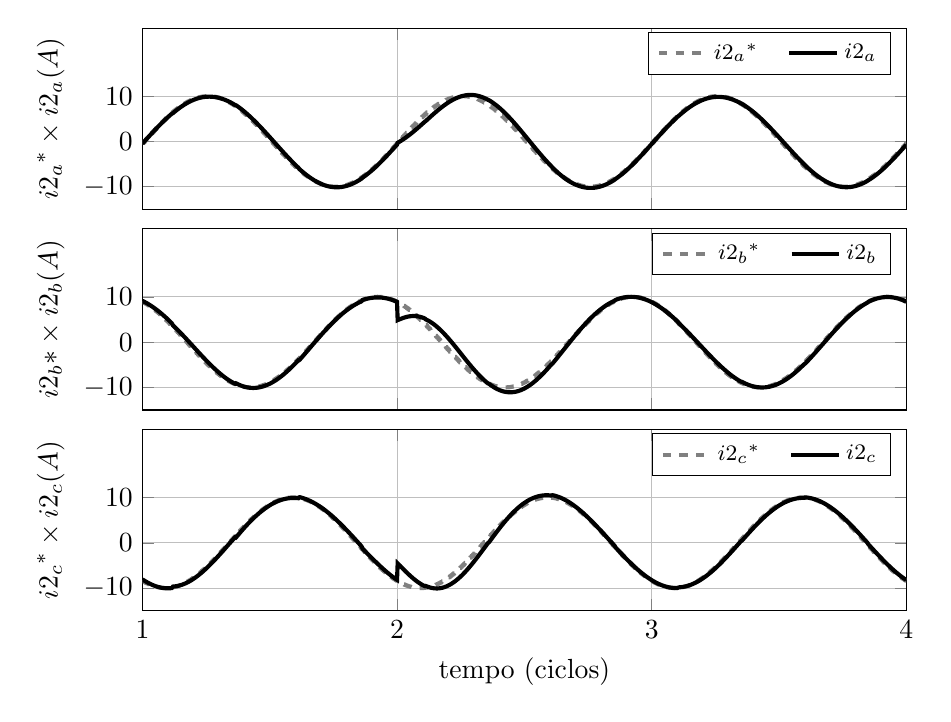
\begin{tikzpicture}

\begin{axis}[%
width=0.8\textwidth,
height=0.189701500343624\textwidth,
scale only axis,
xmin=0.0166666666666667,
xmax=0.0666666666666667,
xtick={0.0166666666666667,0.0333333333333333,0.05,0.0666666666666667},
xticklabels={\empty},
xmajorgrids,
ymin=-15,
ymax=25,
ytick={-10,   0,  10},
ylabel={${\text{i2}_\text{b}}\text{* }\times\text{ i2}_\text{b}\text{ (A)}$},
ymajorgrids,
name=plot2,
legend style={draw=black,fill=white,legend cell align=left},
scaled x ticks = false,
legend columns=-1,
legend style={/tikz/every even column/.append style={column sep=0.3cm}},
legend style={font=\footnotesize}
]
\addplot [color=gray,dashed,line width=1.5pt]
  table[row sep=crcr]{0.0166583333333333	8.95711760239421\\
0.0167	8.81303452065\\
0.0167416666666667	8.81303452065\\
0.0167833333333333	8.66025403784447\\
0.016825	8.66025403784447\\
0.0168666666666667	8.49892692986872\\
0.0169083333333333	8.49892692986872\\
0.01695	8.32921240710107\\
0.0169916666666667	8.32921240710107\\
0.0170333333333333	8.15127795728562\\
0.017075	8.15127795728562\\
0.0171166666666667	7.96529918024204\\
0.0171583333333333	7.96529918024204\\
0.0172	7.77145961456979\\
0.0172416666666667	7.77145961456979\\
0.0172833333333333	7.56995055651764\\
0.017325	7.56995055651764\\
0.0173666666666667	7.36097087119742\\
0.0174083333333333	7.36097087119742\\
0.01745	7.1447267963281\\
0.0174916666666667	7.1447267963281\\
0.0175333333333333	6.92143173870414\\
0.017575	6.92143173870414\\
0.0176166666666667	6.69130606358865\\
0.0176583333333333	6.69130606358865\\
0.0177	6.45457687723957\\
0.0177416666666667	6.45457687723957\\
0.0177833333333333	6.21147780278317\\
0.017825	6.21147780278317\\
0.0178666666666667	5.96224874965622\\
0.0179083333333333	5.96224874965622\\
0.01795	5.70713567684438\\
0.0179916666666667	5.70713567684438\\
0.0180333333333333	5.44639035015033\\
0.018075	5.44639035015033\\
0.0181166666666667	5.18027009373136\\
0.0181583333333333	5.18027009373136\\
0.0182	4.90903753615147\\
0.0182416666666667	4.90903753615147\\
0.0182833333333333	4.63296035119867\\
0.018325	4.63296035119867\\
0.0183666666666667	4.35231099372333\\
0.0184083333333333	4.35231099372333\\
0.01845	4.06736643075805\\
0.0184916666666667	4.06736643075805\\
0.0185333333333333	3.77840786818472\\
0.018575	3.77840786818472\\
0.0186166666666667	3.4857204732182\\
0.0186583333333333	3.4857204732182\\
0.0187	3.18959309298074\\
0.0187416666666667	3.18959309298074\\
0.0187833333333333	2.89031796944476\\
0.018825	2.89031796944476\\
0.0188666666666667	2.58819045102524\\
0.0189083333333333	2.58819045102524\\
0.01895	2.28350870110659\\
0.0189916666666667	2.28350870110659\\
0.0190333333333333	1.97657340379129\\
0.019075	1.97657340379129\\
0.0191166666666667	1.66768746716105\\
0.0191583333333333	1.66768746716105\\
0.0192	1.35715572434307\\
0.0192416666666667	1.35715572434307\\
0.0192833333333333	1.04528463267656\\
0.019325	1.04528463267656\\
0.0193666666666667	0.732381971276336\\
0.0194083333333333	0.732381971276336\\
0.01945	0.418756537292012\\
0.0194916666666667	0.418756537292012\\
0.0195333333333333	0.104717841162471\\
0.019575	0.104717841162471\\
0.0196166666666667	-0.20942419883356\\
0.0196583333333333	-0.20942419883356\\
0.0197	-0.523359562429432\\
0.0197416666666667	-0.523359562429432\\
0.0197833333333333	-0.836778433323152\\
0.019825	-0.836778433323152\\
0.0198666666666667	-1.14937150492867\\
0.0199083333333333	-1.14937150492867\\
0.01995	-1.46083028562412\\
0.0199916666666667	-1.46083028562412\\
0.0200333333333333	-1.77084740319584\\
0.020075	-1.77084740319584\\
0.0201166666666667	-2.0791169081776\\
0.0201583333333333	-2.0791169081776\\
0.0202	-2.38533457578582\\
0.0202416666666667	-2.38533457578582\\
0.0202833333333333	-2.68919820615267\\
0.020325	-2.68919820615267\\
0.0203666666666667	-2.99040792256089\\
0.0204083333333333	-2.99040792256089\\
0.02045	-3.28866646738586\\
0.0204916666666667	-3.28866646738586\\
0.0205333333333333	-3.58367949545303\\
0.020575	-3.58367949545303\\
0.0206166666666667	-3.87515586452106\\
0.0206583333333333	-3.87515586452106\\
0.0207	-4.16280792260405\\
0.0207416666666667	-4.16280792260405\\
0.0207833333333333	-4.44635179184931\\
0.020825	-4.44635179184931\\
0.0208666666666667	-4.72550764869058\\
0.0209083333333333	-4.72550764869058\\
0.02095	-5.00000000000005\\
0.0209916666666667	-5.00000000000005\\
0.0210333333333333	-5.26955795496682\\
0.021075	-5.26955795496682\\
0.0211166666666667	-5.53391549243349\\
0.0211583333333333	-5.53391549243349\\
0.0212	-5.79281172342684\\
0.0212416666666667	-5.79281172342684\\
0.0212833333333333	-6.0459911486238\\
0.021325	-6.0459911486238\\
0.0213666666666667	-6.29320391049844\\
0.0214083333333333	-6.29320391049844\\
0.02145	-6.53420603990112\\
0.0214916666666667	-6.53420603990112\\
0.0215333333333333	-6.76875969682667\\
0.021575	-6.76875969682667\\
0.0216166666666667	-6.99663340513372\\
0.0216583333333333	-6.99663340513372\\
0.0217	-7.2176022809837\\
0.0217416666666667	-7.2176022809837\\
0.0217833333333333	-7.43144825477402\\
0.021825	-7.43144825477402\\
0.0218666666666667	-7.6379602863465\\
0.0219083333333333	-7.6379602863465\\
0.02195	-7.83693457325848\\
0.0219916666666667	-7.83693457325848\\
0.0220333333333333	-8.02817475191123\\
0.022075	-8.02817475191123\\
0.0221166666666667	-8.21149209133713\\
0.0221583333333333	-8.21149209133713\\
0.0222	-8.38670567945433\\
0.0222416666666667	-8.38670567945433\\
0.0222833333333333	-8.55364260160516\\
0.022325	-8.55364260160516\\
0.0223666666666667	-8.71213811120199\\
0.0224083333333333	-8.71213811120199\\
0.02245	-8.86203579231225\\
0.0224916666666667	-8.86203579231225\\
0.0225333333333333	-9.00318771402204\\
0.022575	-9.00318771402204\\
0.0226166666666667	-9.13545457642611\\
0.0226583333333333	-9.13545457642611\\
0.0227	-9.25870584810006\\
0.0227416666666667	-9.25870584810006\\
0.0227833333333333	-9.37281989491902\\
0.022825	-9.37281989491902\\
0.0228666666666667	-9.47768410009597\\
0.0229083333333333	-9.47768410009597\\
0.02295	-9.57319497532079\\
0.0229916666666667	-9.57319497532079\\
0.0230333333333333	-9.6592582628908\\
0.023075	-9.6592582628908\\
0.0231166666666667	-9.73578902873172\\
0.0231583333333333	-9.73578902873172\\
0.0232	-9.80271174621734\\
0.0232416666666667	-9.80271174621734\\
0.0232833333333333	-9.85996037070517\\
0.023325	-9.85996037070517\\
0.0233666666666667	-9.90747840471456\\
0.0234083333333333	-9.90747840471456\\
0.02345	-9.94521895368285\\
0.0234916666666667	-9.94521895368285\\
0.0235333333333333	-9.97314477224471\\
0.023575	-9.97314477224471\\
0.0236166666666667	-9.99122830098871\\
0.0236583333333333	-9.99122830098871\\
0.0237	-9.99945169365525\\
0.0237416666666667	-9.99945169365525\\
0.0237833333333333	-9.99780683474858\\
0.023825	-9.99780683474858\\
0.0238666666666667	-9.98629534754587\\
0.0239083333333333	-9.98629534754587\\
0.02395	-9.96492859249517\\
0.0239916666666667	-9.96492859249517\\
0.0240333333333333	-9.93372765600409\\
0.024075	-9.93372765600409\\
0.0241166666666667	-9.89272332963001\\
0.0241583333333333	-9.89272332963001\\
0.0242	-9.84195607969255\\
0.0242416666666667	-9.84195607969255\\
0.0242833333333333	-9.78147600733818\\
0.024325	-9.78147600733818\\
0.0243666666666667	-9.71134279909649\\
0.0244083333333333	-9.71134279909649\\
0.02445	-9.63162566797671\\
0.0244916666666667	-9.63162566797671\\
0.0245333333333333	-9.5424032851629\\
0.024575	-9.5424032851629\\
0.0246166666666667	-9.44376370237494\\
0.0246583333333333	-9.44376370237494\\
0.0247	-9.33580426497215\\
0.0247416666666667	-9.33580426497215\\
0.0247833333333333	-9.21863151588513\\
0.024825	-9.21863151588513\\
0.0248666666666667	-9.09236109047081\\
0.0249083333333333	-9.09236109047081\\
0.02495	-8.95711760239425\\
0.0249916666666667	-8.95711760239425\\
0.0250333333333333	-8.81303452065005\\
0.025075	-8.81303452065005\\
0.0251166666666667	-8.66025403784451\\
0.0251583333333333	-8.66025403784451\\
0.0252	-8.49892692986876\\
0.0252416666666667	-8.49892692986876\\
0.0252833333333333	-8.32921240710111\\
0.025325	-8.32921240710111\\
0.0253666666666667	-8.15127795728566\\
0.0254083333333333	-8.15127795728566\\
0.02545	-7.96529918024207\\
0.0254916666666667	-7.96529918024207\\
0.0255333333333333	-7.77145961456982\\
0.025575	-7.77145961456982\\
0.0256166666666667	-7.56995055651767\\
0.0256583333333333	-7.56995055651767\\
0.0257	-7.36097087119745\\
0.0257416666666667	-7.36097087119745\\
0.0257833333333333	-7.14472679632814\\
0.025825	-7.14472679632814\\
0.0258666666666667	-6.92143173870417\\
0.0259083333333333	-6.92143173870417\\
0.02595	-6.69130606358868\\
0.0259916666666667	-6.69130606358868\\
0.0260333333333333	-6.4545768772396\\
0.026075	-6.4545768772396\\
0.0261166666666667	-6.2114778027832\\
0.0261583333333333	-6.2114778027832\\
0.0262	-5.96224874965625\\
0.0262416666666667	-5.96224874965625\\
0.0262833333333333	-5.70713567684441\\
0.026325	-5.70713567684441\\
0.0263666666666667	-5.44639035015036\\
0.0264083333333333	-5.44639035015036\\
0.02645	-5.18027009373139\\
0.0264916666666667	-5.18027009373139\\
0.0265333333333333	-4.90903753615149\\
0.026575	-4.90903753615149\\
0.0266166666666667	-4.6329603511987\\
0.0266583333333333	-4.6329603511987\\
0.0267	-4.35231099372335\\
0.0267416666666667	-4.35231099372335\\
0.0267833333333333	-4.06736643075807\\
0.026825	-4.06736643075807\\
0.0268666666666667	-3.77840786818474\\
0.0269083333333333	-3.77840786818474\\
0.02695	-3.48572047321821\\
0.0269916666666667	-3.48572047321821\\
0.0270333333333333	-3.18959309298076\\
0.027075	-3.18959309298076\\
0.0271166666666667	-2.89031796944477\\
0.0271583333333333	-2.89031796944477\\
0.0272	-2.58819045102526\\
0.0272416666666667	-2.58819045102526\\
0.0272833333333333	-2.28350870110661\\
0.027325	-2.28350870110661\\
0.0273666666666667	-1.9765734037913\\
0.0274083333333333	-1.9765734037913\\
0.02745	-1.66768746716106\\
0.0274916666666667	-1.66768746716106\\
0.0275333333333333	-1.35715572434308\\
0.027575	-1.35715572434308\\
0.0276166666666667	-1.04528463267656\\
0.0276583333333333	-1.04528463267656\\
0.0277	-0.732381971276341\\
0.0277416666666667	-0.732381971276341\\
0.0277833333333333	-0.418756537292015\\
0.027825	-0.418756537292015\\
0.0278666666666667	-0.104717841162473\\
0.0279083333333333	-0.104717841162473\\
0.02795	0.209424198833559\\
0.0279916666666667	0.209424198833559\\
0.0280333333333333	0.523359562429433\\
0.028075	0.523359562429433\\
0.0281166666666667	0.836778433323154\\
0.0281583333333333	0.836778433323154\\
0.0282	1.14937150492867\\
0.0282416666666667	1.14937150492867\\
0.0282833333333333	1.46083028562412\\
0.028325	1.46083028562412\\
0.0283666666666667	1.77084740319585\\
0.0284083333333333	1.77084740319585\\
0.02845	2.07911690817761\\
0.0284916666666667	2.07911690817761\\
0.0285333333333333	2.38533457578583\\
0.028575	2.38533457578583\\
0.0286166666666667	2.68919820615268\\
0.0286583333333333	2.68919820615268\\
0.0287	2.9904079225609\\
0.0287416666666667	2.9904079225609\\
0.0287833333333333	3.28866646738587\\
0.028825	3.28866646738587\\
0.0288666666666667	3.58367949545304\\
0.0289083333333333	3.58367949545304\\
0.02895	3.87515586452107\\
0.0289916666666667	3.87515586452107\\
0.0290333333333333	4.16280792260406\\
0.029075	4.16280792260406\\
0.0291166666666667	4.44635179184933\\
0.0291583333333333	4.44635179184933\\
0.0292	4.7255076486906\\
0.0292416666666667	4.7255076486906\\
0.0292833333333333	5.00000000000006\\
0.029325	5.00000000000006\\
0.0293666666666667	5.26955795496684\\
0.0294083333333333	5.26955795496684\\
0.02945	5.53391549243351\\
0.0294916666666667	5.53391549243351\\
0.0295333333333333	5.79281172342686\\
0.029575	5.79281172342686\\
0.0296166666666667	6.04599114862383\\
0.0296583333333333	6.04599114862383\\
0.0297	6.29320391049846\\
0.0297416666666667	6.29320391049846\\
0.0297833333333333	6.53420603990114\\
0.029825	6.53420603990114\\
0.0298666666666667	6.7687596968267\\
0.0299083333333333	6.7687596968267\\
0.02995	6.99663340513375\\
0.0299916666666667	6.99663340513375\\
0.0300333333333333	7.21760228098372\\
0.030075	7.21760228098372\\
0.0301166666666667	7.43144825477405\\
0.0301583333333333	7.43144825477405\\
0.0302	7.63796028634653\\
0.0302416666666667	7.63796028634653\\
0.0302833333333333	7.83693457325851\\
0.030325	7.83693457325851\\
0.0303666666666667	8.02817475191126\\
0.0304083333333333	8.02817475191126\\
0.03045	8.21149209133716\\
0.0304916666666667	8.21149209133716\\
0.0305333333333333	8.38670567945436\\
0.030575	8.38670567945436\\
0.0306166666666667	8.55364260160519\\
0.0306583333333333	8.55364260160519\\
0.0307	8.71213811120203\\
0.0307416666666667	8.71213811120203\\
0.0307833333333333	8.86203579231228\\
0.030825	8.86203579231228\\
0.0308666666666667	9.00318771402207\\
0.0309083333333333	9.00318771402207\\
0.03095	9.13545457642615\\
0.0309916666666667	9.13545457642615\\
0.0310333333333333	9.25870584810009\\
0.031075	9.25870584810009\\
0.0311166666666667	9.37281989491906\\
0.0311583333333333	9.37281989491906\\
0.0312	9.477684100096\\
0.0312416666666667	9.477684100096\\
0.0312833333333333	9.57319497532082\\
0.031325	9.57319497532082\\
0.0313666666666667	9.65925826289084\\
0.0314083333333333	9.65925826289084\\
0.03145	9.73578902873176\\
0.0314916666666667	9.73578902873176\\
0.0315333333333333	9.80271174621738\\
0.031575	9.80271174621738\\
0.0316166666666667	9.85996037070521\\
0.0316583333333333	9.85996037070521\\
0.0317	9.9074784047146\\
0.0317416666666667	9.9074784047146\\
0.0317833333333333	9.94521895368289\\
0.031825	9.94521895368289\\
0.0318666666666667	9.97314477224474\\
0.0319083333333333	9.97314477224474\\
0.03195	9.99122830098875\\
0.0319916666666667	9.99122830098875\\
0.0320333333333333	9.99945169365528\\
0.032075	9.99945169365528\\
0.0321166666666667	9.99780683474862\\
0.0321583333333333	9.99780683474862\\
0.0322	9.98629534754591\\
0.0322416666666667	9.98629534754591\\
0.0322833333333333	9.96492859249521\\
0.032325	9.96492859249521\\
0.0323666666666667	9.93372765600413\\
0.0324083333333333	9.93372765600413\\
0.03245	9.89272332963005\\
0.0324916666666667	9.89272332963005\\
0.0325333333333333	9.84195607969259\\
0.032575	9.84195607969259\\
0.0326166666666667	9.78147600733822\\
0.0326583333333333	9.78147600733822\\
0.0327	9.71134279909653\\
0.0327416666666667	9.71134279909653\\
0.0327833333333333	9.63162566797675\\
0.032825	9.63162566797675\\
0.0328666666666667	9.54240328516294\\
0.0329083333333333	9.54240328516294\\
0.03295	9.44376370237498\\
0.0329916666666667	9.44376370237498\\
0.0330333333333333	9.33580426497218\\
0.033075	9.33580426497218\\
0.0331166666666667	9.21863151588517\\
0.0331583333333333	9.21863151588517\\
0.0332	9.09236109047085\\
0.0332416666666667	9.09236109047085\\
0.0332833333333333	8.95711760239429\\
0.033325	8.95711760239429\\
0.0333666666666667	8.81303452065008\\
0.0334083333333333	8.81303452065008\\
0.03345	8.66025403784455\\
0.0334916666666667	8.66025403784455\\
0.0335333333333333	8.49892692986879\\
0.033575	8.49892692986879\\
0.0336166666666667	8.32921240710115\\
0.0336583333333333	8.32921240710115\\
0.0337	8.15127795728569\\
0.0337416666666667	8.15127795728569\\
0.0337833333333333	7.96529918024211\\
0.033825	7.96529918024211\\
0.0338666666666667	7.77145961456986\\
0.0339083333333333	7.77145961456986\\
0.03395	7.56995055651771\\
0.0339916666666667	7.56995055651771\\
0.0340333333333333	7.36097087119748\\
0.034075	7.36097087119748\\
0.0341166666666667	7.14472679632817\\
0.0341583333333333	7.14472679632817\\
0.0342	6.9214317387042\\
0.0342416666666667	6.9214317387042\\
0.0342833333333333	6.69130606358871\\
0.034325	6.69130606358871\\
0.0343666666666667	6.45457687723963\\
0.0344083333333333	6.45457687723963\\
0.03445	6.21147780278323\\
0.0344916666666667	6.21147780278323\\
0.0345333333333333	5.96224874965628\\
0.034575	5.96224874965628\\
0.0346166666666667	5.70713567684443\\
0.0346583333333333	5.70713567684443\\
0.0347	5.44639035015038\\
0.0347416666666667	5.44639035015038\\
0.0347833333333333	5.18027009373141\\
0.034825	5.18027009373141\\
0.0348666666666667	4.90903753615151\\
0.0349083333333333	4.90903753615151\\
0.03495	4.63296035119872\\
0.0349916666666667	4.63296035119872\\
0.0350333333333333	4.35231099372337\\
0.035075	4.35231099372337\\
0.0351166666666667	4.06736643075809\\
0.0351583333333333	4.06736643075809\\
0.0352	3.77840786818476\\
0.0352416666666667	3.77840786818476\\
0.0352833333333333	3.48572047321823\\
0.035325	3.48572047321823\\
0.0353666666666667	3.18959309298077\\
0.0354083333333333	3.18959309298077\\
0.03545	2.89031796944478\\
0.0354916666666667	2.89031796944478\\
0.0355333333333333	2.58819045102527\\
0.035575	2.58819045102527\\
0.0356166666666667	2.28350870110662\\
0.0356583333333333	2.28350870110662\\
0.0357	1.97657340379131\\
0.0357416666666667	1.97657340379131\\
0.0357833333333333	1.66768746716107\\
0.035825	1.66768746716107\\
0.0358666666666667	1.35715572434309\\
0.0359083333333333	1.35715572434309\\
0.03595	1.04528463267657\\
0.0359916666666667	1.04528463267657\\
0.0360333333333333	0.732381971276348\\
0.036075	0.732381971276348\\
0.0361166666666667	0.418756537292022\\
0.0361583333333333	0.418756537292022\\
0.0362	0.104717841162477\\
0.0362416666666667	0.104717841162477\\
0.0362833333333333	-0.209424198833557\\
0.036325	-0.209424198833557\\
0.0363666666666667	-0.523359562429431\\
0.0364083333333333	-0.523359562429431\\
0.03645	-0.836778433323154\\
0.0364916666666667	-0.836778433323154\\
0.0365333333333333	-1.14937150492867\\
0.036575	-1.14937150492867\\
0.0366166666666667	-1.46083028562413\\
0.0366583333333333	-1.46083028562413\\
0.0367	-1.77084740319585\\
0.0367416666666667	-1.77084740319585\\
0.0367833333333333	-2.07911690817762\\
0.036825	-2.07911690817762\\
0.0368666666666667	-2.38533457578584\\
0.0369083333333333	-2.38533457578584\\
0.03695	-2.68919820615269\\
0.0369916666666667	-2.68919820615269\\
0.0370333333333333	-2.99040792256091\\
0.037075	-2.99040792256091\\
0.0371166666666667	-3.28866646738588\\
0.0371583333333333	-3.28866646738588\\
0.0372	-3.58367949545306\\
0.0372416666666667	-3.58367949545306\\
0.0372833333333333	-3.87515586452109\\
0.037325	-3.87515586452109\\
0.0373666666666667	-4.16280792260408\\
0.0374083333333333	-4.16280792260408\\
0.03745	-4.44635179184934\\
0.0374916666666667	-4.44635179184934\\
0.0375333333333333	-4.72550764869062\\
0.037575	-4.72550764869062\\
0.0376166666666667	-5.00000000000008\\
0.0376583333333333	-5.00000000000008\\
0.0377	-5.26955795496686\\
0.0377416666666667	-5.26955795496686\\
0.0377833333333333	-5.53391549243353\\
0.037825	-5.53391549243353\\
0.0378666666666667	-5.79281172342689\\
0.0379083333333333	-5.79281172342689\\
0.03795	-6.04599114862385\\
0.0379916666666667	-6.04599114862385\\
0.0380333333333333	-6.29320391049848\\
0.038075	-6.29320391049848\\
0.0381166666666667	-6.53420603990117\\
0.0381583333333333	-6.53420603990117\\
0.0382	-6.76875969682673\\
0.0382416666666667	-6.76875969682673\\
0.0382833333333333	-6.99663340513378\\
0.038325	-6.99663340513378\\
0.0383666666666667	-7.21760228098375\\
0.0384083333333333	-7.21760228098375\\
0.03845	-7.43144825477408\\
0.0384916666666667	-7.43144825477408\\
0.0385333333333333	-7.63796028634656\\
0.038575	-7.63796028634656\\
0.0386166666666667	-7.83693457325854\\
0.0386583333333333	-7.83693457325854\\
0.0387	-8.02817475191129\\
0.0387416666666667	-8.02817475191129\\
0.0387833333333333	-8.21149209133719\\
0.038825	-8.21149209133719\\
0.0388666666666667	-8.3867056794544\\
0.0389083333333333	-8.3867056794544\\
0.03895	-8.55364260160523\\
0.0389916666666667	-8.55364260160523\\
0.0390333333333333	-8.71213811120206\\
0.039075	-8.71213811120206\\
0.0391166666666667	-8.86203579231232\\
0.0391583333333333	-8.86203579231232\\
0.0392	-9.00318771402211\\
0.0392416666666667	-9.00318771402211\\
0.0392833333333333	-9.13545457642618\\
0.039325	-9.13545457642618\\
0.0393666666666667	-9.25870584810013\\
0.0394083333333333	-9.25870584810013\\
0.03945	-9.3728198949191\\
0.0394916666666667	-9.3728198949191\\
0.0395333333333333	-9.47768410009604\\
0.039575	-9.47768410009604\\
0.0396166666666667	-9.57319497532086\\
0.0396583333333333	-9.57319497532086\\
0.0397	-9.65925826289087\\
0.0397416666666667	-9.65925826289087\\
0.0397833333333333	-9.7357890287318\\
0.039825	-9.7357890287318\\
0.0398666666666667	-9.80271174621742\\
0.0399083333333333	-9.80271174621742\\
0.03995	-9.85996037070525\\
0.0399916666666667	-9.85996037070525\\
0.0400333333333333	-9.90747840471464\\
0.040075	-9.90747840471464\\
0.0401166666666667	-9.94521895368294\\
0.0401583333333333	-9.94521895368294\\
0.0402	-9.97314477224478\\
0.0402416666666667	-9.97314477224478\\
0.0402833333333333	-9.99122830098879\\
0.040325	-9.99122830098879\\
0.0403666666666667	-9.99945169365533\\
0.0404083333333333	-9.99945169365533\\
0.04045	-9.99780683474866\\
0.0404916666666667	-9.99780683474866\\
0.0405333333333333	-9.98629534754595\\
0.040575	-9.98629534754595\\
0.0406166666666667	-9.96492859249525\\
0.0406583333333333	-9.96492859249525\\
0.0407	-9.93372765600417\\
0.0407416666666667	-9.93372765600417\\
0.0407833333333333	-9.89272332963009\\
0.040825	-9.89272332963009\\
0.0408666666666667	-9.84195607969263\\
0.0409083333333333	-9.84195607969263\\
0.04095	-9.78147600733827\\
0.0409916666666667	-9.78147600733827\\
0.0410333333333333	-9.71134279909657\\
0.041075	-9.71134279909657\\
0.0411166666666667	-9.63162566797679\\
0.0411583333333333	-9.63162566797679\\
0.0412	-9.54240328516298\\
0.0412416666666667	-9.54240328516298\\
0.0412833333333333	-9.44376370237502\\
0.041325	-9.44376370237502\\
0.0413666666666667	-9.33580426497222\\
0.0414083333333333	-9.33580426497222\\
0.04145	-9.21863151588521\\
0.0414916666666667	-9.21863151588521\\
0.0415333333333333	-9.09236109047089\\
0.041575	-9.09236109047089\\
0.0416166666666667	-8.95711760239433\\
0.0416583333333333	-8.95711760239433\\
0.0417	-8.81303452065012\\
0.0417416666666667	-8.81303452065012\\
0.0417833333333333	-8.66025403784458\\
0.041825	-8.66025403784458\\
0.0418666666666667	-8.49892692986883\\
0.0419083333333333	-8.49892692986883\\
0.04195	-8.32921240710118\\
0.0419916666666667	-8.32921240710118\\
0.0420333333333333	-8.15127795728573\\
0.042075	-8.15127795728573\\
0.0421166666666667	-7.96529918024214\\
0.0421583333333333	-7.96529918024214\\
0.0422	-7.77145961456989\\
0.0422416666666667	-7.77145961456989\\
0.0422833333333333	-7.56995055651774\\
0.042325	-7.56995055651774\\
0.0423666666666667	-7.36097087119751\\
0.0424083333333333	-7.36097087119751\\
0.04245	-7.1447267963282\\
0.0424916666666667	-7.1447267963282\\
0.0425333333333333	-6.92143173870423\\
0.042575	-6.92143173870423\\
0.0426166666666667	-6.69130606358874\\
0.0426583333333333	-6.69130606358874\\
0.0427	-6.45457687723966\\
0.0427416666666667	-6.45457687723966\\
0.0427833333333333	-6.21147780278325\\
0.042825	-6.21147780278325\\
0.0428666666666667	-5.9622487496563\\
0.0429083333333333	-5.9622487496563\\
0.04295	-5.70713567684446\\
0.0429916666666667	-5.70713567684446\\
0.0430333333333333	-5.44639035015041\\
0.043075	-5.44639035015041\\
0.0431166666666667	-5.18027009373143\\
0.0431583333333333	-5.18027009373143\\
0.0432	-4.90903753615153\\
0.0432416666666667	-4.90903753615153\\
0.0432833333333333	-4.63296035119874\\
0.043325	-4.63296035119874\\
0.0433666666666667	-4.35231099372339\\
0.0434083333333333	-4.35231099372339\\
0.04345	-4.06736643075811\\
0.0434916666666667	-4.06736643075811\\
0.0435333333333333	-3.77840786818477\\
0.043575	-3.77840786818477\\
0.0436166666666667	-3.48572047321825\\
0.0436583333333333	-3.48572047321825\\
0.0437	-3.18959309298079\\
0.0437416666666667	-3.18959309298079\\
0.0437833333333333	-2.8903179694448\\
0.043825	-2.8903179694448\\
0.0438666666666667	-2.58819045102528\\
0.0439083333333333	-2.58819045102528\\
0.04395	-2.28350870110663\\
0.0439916666666667	-2.28350870110663\\
0.0440333333333333	-1.97657340379133\\
0.044075	-1.97657340379133\\
0.0441166666666667	-1.66768746716108\\
0.0441583333333333	-1.66768746716108\\
0.0442	-1.35715572434309\\
0.0442416666666667	-1.35715572434309\\
0.0442833333333333	-1.04528463267658\\
0.044325	-1.04528463267658\\
0.0443666666666667	-0.732381971276353\\
0.0444083333333333	-0.732381971276353\\
0.04445	-0.418756537292025\\
0.0444916666666667	-0.418756537292025\\
0.0445333333333333	-0.104717841162479\\
0.044575	-0.104717841162479\\
0.0446166666666667	0.209424198833555\\
0.0446583333333333	0.209424198833555\\
0.0447	0.523359562429432\\
0.0447416666666667	0.523359562429432\\
0.0447833333333333	0.836778433323156\\
0.044825	0.836778433323156\\
0.0448666666666667	1.14937150492867\\
0.0449083333333333	1.14937150492867\\
0.04495	1.46083028562413\\
0.0449916666666667	1.46083028562413\\
0.0450333333333333	1.77084740319586\\
0.045075	1.77084740319586\\
0.0451166666666667	2.07911690817762\\
0.0451583333333333	2.07911690817762\\
0.0452	2.38533457578585\\
0.0452416666666667	2.38533457578585\\
0.0452833333333333	2.6891982061527\\
0.045325	2.6891982061527\\
0.0453666666666667	2.99040792256092\\
0.0454083333333333	2.99040792256092\\
0.04545	3.28866646738589\\
0.0454916666666667	3.28866646738589\\
0.0455333333333333	3.58367949545307\\
0.045575	3.58367949545307\\
0.0456166666666667	3.8751558645211\\
0.0456583333333333	3.8751558645211\\
0.0457	4.16280792260409\\
0.0457416666666667	4.16280792260409\\
0.0457833333333333	4.44635179184936\\
0.045825	4.44635179184936\\
0.0458666666666667	4.72550764869064\\
0.0459083333333333	4.72550764869064\\
0.04595	5.0000000000001\\
0.0459916666666667	5.0000000000001\\
0.0460333333333333	5.26955795496689\\
0.046075	5.26955795496689\\
0.0461166666666667	5.53391549243356\\
0.0461583333333333	5.53391549243356\\
0.0462	5.79281172342691\\
0.0462416666666667	5.79281172342691\\
0.0462833333333333	6.04599114862388\\
0.046325	6.04599114862388\\
0.0463666666666667	6.29320391049851\\
0.0464083333333333	6.29320391049851\\
0.04645	6.5342060399012\\
0.0464916666666667	6.5342060399012\\
0.0465333333333333	6.76875969682676\\
0.046575	6.76875969682676\\
0.0466166666666667	6.99663340513381\\
0.0466583333333333	6.99663340513381\\
0.0467	7.21760228098379\\
0.0467416666666667	7.21760228098379\\
0.0467833333333333	7.43144825477411\\
0.046825	7.43144825477411\\
0.0468666666666667	7.6379602863466\\
0.0469083333333333	7.6379602863466\\
0.04695	7.83693457325858\\
0.0469916666666667	7.83693457325858\\
0.0470333333333333	8.02817475191133\\
0.047075	8.02817475191133\\
0.0471166666666667	8.21149209133723\\
0.0471583333333333	8.21149209133723\\
0.0472	8.38670567945444\\
0.0472416666666667	8.38670567945444\\
0.0472833333333333	8.55364260160527\\
0.047325	8.55364260160527\\
0.0473666666666667	8.7121381112021\\
0.0474083333333333	8.7121381112021\\
0.04745	8.86203579231236\\
0.0474916666666667	8.86203579231236\\
0.0475333333333333	9.00318771402215\\
0.047575	9.00318771402215\\
0.0476166666666667	9.13545457642623\\
0.0476583333333333	9.13545457642623\\
0.0477	9.25870584810017\\
0.0477416666666667	9.25870584810017\\
0.0477833333333333	9.37281989491914\\
0.047825	9.37281989491914\\
0.0478666666666667	9.47768410009609\\
0.0479083333333333	9.47768410009609\\
0.04795	9.57319497532091\\
0.0479916666666667	9.57319497532091\\
0.0480333333333333	9.65925826289092\\
0.048075	9.65925826289092\\
0.0481166666666667	9.73578902873184\\
0.0481583333333333	9.73578902873184\\
0.0482	9.80271174621746\\
0.0482416666666667	9.80271174621746\\
0.0482833333333333	9.85996037070529\\
0.048325	9.85996037070529\\
0.0483666666666667	9.90747840471468\\
0.0484083333333333	9.90747840471468\\
0.04845	9.94521895368298\\
0.0484916666666667	9.94521895368298\\
0.0485333333333333	9.97314477224483\\
0.048575	9.97314477224483\\
0.0486166666666667	9.99122830098883\\
0.0486583333333333	9.99122830098883\\
0.0487	9.99945169365537\\
0.0487416666666667	9.99945169365537\\
0.0487833333333333	9.99780683474871\\
0.048825	9.99780683474871\\
0.0488666666666667	9.98629534754599\\
0.0489083333333333	9.98629534754599\\
0.04895	9.9649285924953\\
0.0489916666666667	9.9649285924953\\
0.0490333333333333	9.93372765600422\\
0.049075	9.93372765600422\\
0.0491166666666667	9.89272332963014\\
0.0491583333333333	9.89272332963014\\
0.0492	9.84195607969268\\
0.0492416666666667	9.84195607969268\\
0.0492833333333333	9.78147600733831\\
0.049325	9.78147600733831\\
0.0493666666666667	9.71134279909661\\
0.0494083333333333	9.71134279909661\\
0.04945	9.63162566797684\\
0.0494916666666667	9.63162566797684\\
0.0495333333333333	9.54240328516302\\
0.049575	9.54240328516302\\
0.0496166666666667	9.44376370237506\\
0.0496583333333333	9.44376370237506\\
0.0497	9.33580426497227\\
0.0497416666666667	9.33580426497227\\
0.0497833333333333	9.21863151588525\\
0.049825	9.21863151588525\\
0.0498666666666667	9.09236109047093\\
0.0499083333333333	9.09236109047093\\
0.04995	8.95711760239437\\
0.0499916666666667	8.95711760239437\\
0.0500333333333333	8.81303452065016\\
0.050075	8.81303452065016\\
0.0501166666666667	8.66025403784462\\
0.0501583333333333	8.66025403784462\\
0.0502	8.49892692986887\\
0.0502416666666667	8.49892692986887\\
0.0502833333333333	8.32921240710123\\
0.050325	8.32921240710123\\
0.0503666666666667	8.15127795728577\\
0.0504083333333333	8.15127795728577\\
0.05045	7.96529918024218\\
0.0504916666666667	7.96529918024218\\
0.0505333333333333	7.77145961456993\\
0.050575	7.77145961456993\\
0.0506166666666667	7.56995055651778\\
0.0506583333333333	7.56995055651778\\
0.0507	7.36097087119755\\
0.0507416666666667	7.36097087119755\\
0.0507833333333333	7.14472679632824\\
0.050825	7.14472679632824\\
0.0508666666666667	6.92143173870427\\
0.0509083333333333	6.92143173870427\\
0.05095	6.69130606358878\\
0.0509916666666667	6.69130606358878\\
0.0510333333333333	6.45457687723969\\
0.051075	6.45457687723969\\
0.0511166666666667	6.21147780278329\\
0.0511583333333333	6.21147780278329\\
0.0512	5.96224874965633\\
0.0512416666666667	5.96224874965633\\
0.0512833333333333	5.70713567684449\\
0.051325	5.70713567684449\\
0.0513666666666667	5.44639035015043\\
0.0514083333333333	5.44639035015043\\
0.05145	5.18027009373146\\
0.0514916666666667	5.18027009373146\\
0.0515333333333333	4.90903753615156\\
0.051575	4.90903753615156\\
0.0516166666666667	4.63296035119876\\
0.0516583333333333	4.63296035119876\\
0.0517	4.35231099372341\\
0.0517416666666667	4.35231099372341\\
0.0517833333333333	4.06736643075813\\
0.051825	4.06736643075813\\
0.0518666666666667	3.77840786818479\\
0.0519083333333333	3.77840786818479\\
0.05195	3.48572047321827\\
0.0519916666666667	3.48572047321827\\
0.0520333333333333	3.18959309298081\\
0.052075	3.18959309298081\\
0.0521166666666667	2.89031796944481\\
0.0521583333333333	2.89031796944481\\
0.0522	2.5881904510253\\
0.0522416666666667	2.5881904510253\\
0.0522833333333333	2.28350870110664\\
0.052325	2.28350870110664\\
0.0523666666666667	1.97657340379134\\
0.0524083333333333	1.97657340379134\\
0.05245	1.66768746716109\\
0.0524916666666667	1.66768746716109\\
0.0525333333333333	1.3571557243431\\
0.052575	1.3571557243431\\
0.0526166666666667	1.04528463267659\\
0.0526583333333333	1.04528463267659\\
0.0527	0.73238197127636\\
0.0527416666666667	0.73238197127636\\
0.0527833333333333	0.418756537292029\\
0.052825	0.418756537292029\\
0.0528666666666667	0.104717841162482\\
0.0529083333333333	0.104717841162482\\
0.05295	-0.209424198833554\\
0.0529916666666667	-0.209424198833554\\
0.0530333333333333	-0.523359562429432\\
0.053075	-0.523359562429432\\
0.0531166666666667	-0.836778433323157\\
0.0531583333333333	-0.836778433323157\\
0.0532	-1.14937150492868\\
0.0532416666666667	-1.14937150492868\\
0.0532833333333333	-1.46083028562414\\
0.053325	-1.46083028562414\\
0.0533666666666667	-1.77084740319586\\
0.0534083333333333	-1.77084740319586\\
0.05345	-2.07911690817763\\
0.0534916666666667	-2.07911690817763\\
0.0535333333333333	-2.38533457578585\\
0.053575	-2.38533457578585\\
0.0536166666666667	-2.68919820615271\\
0.0536583333333333	-2.68919820615271\\
0.0537	-2.99040792256093\\
0.0537416666666667	-2.99040792256093\\
0.0537833333333333	-3.2886664673859\\
0.053825	-3.2886664673859\\
0.0538666666666667	-3.58367949545308\\
0.0539083333333333	-3.58367949545308\\
0.05395	-3.87515586452112\\
0.0539916666666667	-3.87515586452112\\
0.0540333333333333	-4.16280792260411\\
0.054075	-4.16280792260411\\
0.0541166666666667	-4.44635179184938\\
0.0541583333333333	-4.44635179184938\\
0.0542	-4.72550764869065\\
0.0542416666666667	-4.72550764869065\\
0.0542833333333333	-5.00000000000012\\
0.054325	-5.00000000000012\\
0.0543666666666667	-5.26955795496691\\
0.0544083333333333	-5.26955795496691\\
0.05445	-5.53391549243358\\
0.0544916666666667	-5.53391549243358\\
0.0545333333333333	-5.79281172342693\\
0.054575	-5.79281172342693\\
0.0546166666666667	-6.0459911486239\\
0.0546583333333333	-6.0459911486239\\
0.0547	-6.29320391049854\\
0.0547416666666667	-6.29320391049854\\
0.0547833333333333	-6.53420603990122\\
0.054825	-6.53420603990122\\
0.0548666666666667	-6.76875969682678\\
0.0549083333333333	-6.76875969682678\\
0.05495	-6.99663340513384\\
0.0549916666666667	-6.99663340513384\\
0.0550333333333333	-7.21760228098381\\
0.055075	-7.21760228098381\\
0.0551166666666667	-7.43144825477414\\
0.0551583333333333	-7.43144825477414\\
0.0552	-7.63796028634663\\
0.0552416666666667	-7.63796028634663\\
0.0552833333333333	-7.83693457325861\\
0.055325	-7.83693457325861\\
0.0553666666666667	-8.02817475191136\\
0.0554083333333333	-8.02817475191136\\
0.05545	-8.21149209133726\\
0.0554916666666667	-8.21149209133726\\
0.0555333333333333	-8.38670567945447\\
0.055575	-8.38670567945447\\
0.0556166666666667	-8.5536426016053\\
0.0556583333333333	-8.5536426016053\\
0.0557	-8.71213811120214\\
0.0557416666666667	-8.71213811120214\\
0.0557833333333333	-8.86203579231239\\
0.055825	-8.86203579231239\\
0.0558666666666667	-9.00318771402219\\
0.0559083333333333	-9.00318771402219\\
0.05595	-9.13545457642627\\
0.0559916666666667	-9.13545457642627\\
0.0560333333333333	-9.25870584810021\\
0.056075	-9.25870584810021\\
0.0561166666666667	-9.37281989491918\\
0.0561583333333333	-9.37281989491918\\
0.0562	-9.47768410009613\\
0.0562416666666667	-9.47768410009613\\
0.0562833333333333	-9.57319497532095\\
0.056325	-9.57319497532095\\
0.0563666666666667	-9.65925826289096\\
0.0564083333333333	-9.65925826289096\\
0.05645	-9.73578902873188\\
0.0564916666666667	-9.73578902873188\\
0.0565333333333333	-9.8027117462175\\
0.056575	-9.8027117462175\\
0.0566166666666667	-9.85996037070534\\
0.0566583333333333	-9.85996037070534\\
0.0567	-9.90747840471473\\
0.0567416666666667	-9.90747840471473\\
0.0567833333333333	-9.94521895368302\\
0.056825	-9.94521895368302\\
0.0568666666666667	-9.97314477224487\\
0.0569083333333333	-9.97314477224487\\
0.05695	-9.99122830098888\\
0.0569916666666667	-9.99122830098888\\
0.0570333333333333	-9.99945169365542\\
0.057075	-9.99945169365542\\
0.0571166666666667	-9.99780683474875\\
0.0571583333333333	-9.99780683474875\\
0.0572	-9.98629534754604\\
0.0572416666666667	-9.98629534754604\\
0.0572833333333333	-9.96492859249534\\
0.057325	-9.96492859249534\\
0.0573666666666667	-9.93372765600427\\
0.0574083333333333	-9.93372765600427\\
0.05745	-9.89272332963018\\
0.0574916666666667	-9.89272332963018\\
0.0575333333333333	-9.84195607969272\\
0.057575	-9.84195607969272\\
0.0576166666666667	-9.78147600733836\\
0.0576583333333333	-9.78147600733836\\
0.0577	-9.71134279909666\\
0.0577416666666667	-9.71134279909666\\
0.0577833333333333	-9.63162566797688\\
0.057825	-9.63162566797688\\
0.0578666666666667	-9.54240328516306\\
0.0579083333333333	-9.54240328516306\\
0.05795	-9.44376370237511\\
0.0579916666666667	-9.44376370237511\\
0.0580333333333333	-9.33580426497231\\
0.058075	-9.33580426497231\\
0.0581166666666667	-9.21863151588529\\
0.0581583333333333	-9.21863151588529\\
0.0582	-9.09236109047097\\
0.0582416666666667	-9.09236109047097\\
0.0582833333333333	-8.95711760239441\\
0.058325	-8.95711760239441\\
0.0583666666666667	-8.8130345206502\\
0.0584083333333333	-8.8130345206502\\
0.05845	-8.66025403784466\\
0.0584916666666667	-8.66025403784466\\
0.0585333333333333	-8.49892692986891\\
0.058575	-8.49892692986891\\
0.0586166666666667	-8.32921240710126\\
0.0586583333333333	-8.32921240710126\\
0.0587	-8.1512779572858\\
0.0587416666666667	-8.1512779572858\\
0.0587833333333333	-7.96529918024222\\
0.058825	-7.96529918024222\\
0.0588666666666667	-7.77145961456996\\
0.0589083333333333	-7.77145961456996\\
0.05895	-7.56995055651781\\
0.0589916666666667	-7.56995055651781\\
0.0590333333333333	-7.36097087119758\\
0.059075	-7.36097087119758\\
0.0591166666666667	-7.14472679632827\\
0.0591583333333333	-7.14472679632827\\
0.0592	-6.9214317387043\\
0.0592416666666667	-6.9214317387043\\
0.0592833333333333	-6.69130606358881\\
0.059325	-6.69130606358881\\
0.0593666666666667	-6.45457687723972\\
0.0594083333333333	-6.45457687723972\\
0.05945	-6.21147780278331\\
0.0594916666666667	-6.21147780278331\\
0.0595333333333333	-5.96224874965636\\
0.059575	-5.96224874965636\\
0.0596166666666667	-5.70713567684451\\
0.0596583333333333	-5.70713567684451\\
0.0597	-5.44639035015046\\
0.0597416666666667	-5.44639035015046\\
0.0597833333333333	-5.18027009373148\\
0.059825	-5.18027009373148\\
0.0598666666666667	-4.90903753615158\\
0.0599083333333333	-4.90903753615158\\
0.05995	-4.63296035119878\\
0.0599916666666667	-4.63296035119878\\
0.0600333333333333	-4.35231099372343\\
0.060075	-4.35231099372343\\
0.0601166666666667	-4.06736643075815\\
0.0601583333333333	-4.06736643075815\\
0.0602	-3.77840786818481\\
0.0602416666666667	-3.77840786818481\\
0.0602833333333333	-3.48572047321828\\
0.060325	-3.48572047321828\\
0.0603666666666667	-3.18959309298082\\
0.0604083333333333	-3.18959309298082\\
0.06045	-2.89031796944483\\
0.0604916666666667	-2.89031796944483\\
0.0605333333333333	-2.58819045102531\\
0.060575	-2.58819045102531\\
0.0606166666666667	-2.28350870110665\\
0.0606583333333333	-2.28350870110665\\
0.0607	-1.97657340379135\\
0.0607416666666667	-1.97657340379135\\
0.0607833333333333	-1.6676874671611\\
0.060825	-1.6676874671611\\
0.0608666666666667	-1.35715572434311\\
0.0609083333333333	-1.35715572434311\\
0.06095	-1.04528463267659\\
0.0609916666666667	-1.04528463267659\\
0.0610333333333333	-0.732381971276366\\
0.061075	-0.732381971276366\\
0.0611166666666667	-0.418756537292034\\
0.0611583333333333	-0.418756537292034\\
0.0612	-0.104717841162486\\
0.0612416666666667	-0.104717841162486\\
0.0612833333333333	0.209424198833552\\
0.061325	0.209424198833552\\
0.0613666666666667	0.52335956242943\\
0.0614083333333333	0.52335956242943\\
0.06145	0.836778433323157\\
0.0614916666666667	0.836778433323157\\
0.0615333333333333	1.14937150492868\\
0.061575	1.14937150492868\\
0.0616166666666667	1.46083028562414\\
0.0616583333333333	1.46083028562414\\
0.0617	1.77084740319587\\
0.0617416666666667	1.77084740319587\\
0.0617833333333333	2.07911690817764\\
0.061825	2.07911690817764\\
0.0618666666666667	2.38533457578586\\
0.0619083333333333	2.38533457578586\\
0.06195	2.68919820615272\\
0.0619916666666667	2.68919820615272\\
0.0620333333333333	2.99040792256094\\
0.062075	2.99040792256094\\
0.0621166666666667	3.28866646738591\\
0.0621583333333333	3.28866646738591\\
0.0622	3.5836794954531\\
0.0622416666666667	3.5836794954531\\
0.0622833333333333	3.87515586452113\\
0.062325	3.87515586452113\\
0.0623666666666667	4.16280792260412\\
0.0624083333333333	4.16280792260412\\
0.06245	4.4463517918494\\
0.0624916666666667	4.4463517918494\\
0.0625333333333333	4.72550764869067\\
0.062575	4.72550764869067\\
0.0626166666666667	5.00000000000014\\
0.0626583333333333	5.00000000000014\\
0.0627	5.26955795496693\\
0.0627416666666667	5.26955795496693\\
0.0627833333333333	5.5339154924336\\
0.062825	5.5339154924336\\
0.0628666666666667	5.79281172342696\\
0.0629083333333333	5.79281172342696\\
0.06295	6.04599114862392\\
0.0629916666666667	6.04599114862392\\
0.0630333333333333	6.29320391049856\\
0.063075	6.29320391049856\\
0.0631166666666667	6.53420603990125\\
0.0631583333333333	6.53420603990125\\
0.0632	6.76875969682681\\
0.0632416666666667	6.76875969682681\\
0.0632833333333333	6.99663340513387\\
0.063325	6.99663340513387\\
0.0633666666666667	7.21760228098384\\
0.0634083333333333	7.21760228098384\\
0.06345	7.43144825477417\\
0.0634916666666667	7.43144825477417\\
0.0635333333333333	7.63796028634666\\
0.063575	7.63796028634666\\
0.0636166666666667	7.83693457325864\\
0.0636583333333333	7.83693457325864\\
0.0637	8.0281747519114\\
0.0637416666666667	8.0281747519114\\
0.0637833333333333	8.2114920913373\\
0.063825	8.2114920913373\\
0.0638666666666667	8.3867056794545\\
0.0639083333333333	8.3867056794545\\
0.06395	8.55364260160534\\
0.0639916666666667	8.55364260160534\\
0.0640333333333333	8.71213811120217\\
0.064075	8.71213811120217\\
0.0641166666666667	8.86203579231243\\
0.0641583333333333	8.86203579231243\\
0.0642	9.00318771402222\\
0.0642416666666667	9.00318771402222\\
0.0642833333333333	9.1354545764263\\
0.064325	9.1354545764263\\
0.0643666666666667	9.25870584810025\\
0.0644083333333333	9.25870584810025\\
0.06445	9.37281989491922\\
0.0644916666666667	9.37281989491922\\
0.0645333333333333	9.47768410009616\\
0.064575	9.47768410009616\\
0.0646166666666667	9.57319497532098\\
0.0646583333333333	9.57319497532098\\
0.0647	9.659258262891\\
0.0647416666666667	9.659258262891\\
0.0647833333333333	9.73578902873192\\
0.064825	9.73578902873192\\
0.0648666666666667	9.80271174621754\\
0.0649083333333333	9.80271174621754\\
0.06495	9.85996037070537\\
0.0649916666666667	9.85996037070537\\
0.0650333333333333	9.90747840471476\\
0.065075	9.90747840471476\\
0.0651166666666667	9.94521895368306\\
0.0651583333333333	9.94521895368306\\
0.0652	9.97314477224491\\
0.0652416666666667	9.97314477224491\\
0.0652833333333333	9.99122830098892\\
0.065325	9.99122830098892\\
0.0653666666666667	9.99945169365546\\
0.0654083333333333	9.99945169365546\\
0.06545	9.99780683474879\\
0.0654916666666667	9.99780683474879\\
0.0655333333333333	9.98629534754607\\
0.065575	9.98629534754607\\
0.0656166666666667	9.96492859249538\\
0.0656583333333333	9.96492859249538\\
0.0657	9.9337276560043\\
0.0657416666666667	9.9337276560043\\
0.0657833333333333	9.89272332963022\\
0.065825	9.89272332963022\\
0.0658666666666667	9.84195607969276\\
0.0659083333333333	9.84195607969276\\
0.06595	9.78147600733839\\
0.0659916666666667	9.78147600733839\\
0.0660333333333333	9.71134279909669\\
0.066075	9.71134279909669\\
0.0661166666666667	9.63162566797691\\
0.0661583333333333	9.63162566797691\\
0.0662	9.5424032851631\\
0.0662416666666667	9.5424032851631\\
0.0662833333333333	9.44376370237514\\
0.066325	9.44376370237514\\
0.0663666666666667	9.33580426497234\\
0.0664083333333333	9.33580426497234\\
0.06645	9.21863151588533\\
0.0664916666666667	9.21863151588533\\
0.0665333333333333	9.092361090471\\
0.066575	9.092361090471\\
0.0666166666666667	8.95711760239444\\
0.0666583333333333	8.95711760239444\\
};
\addlegendentry{${\text{i2}_\text{b}}^\text{*}$};

\addplot [color=black,solid,line width=1.5pt]
  table[row sep=crcr]{0.0166583333333333	9.10238729436972\\
0.0167	9.03402165826534\\
0.0167416666666667	8.96368598655141\\
0.0167833333333333	8.89133568061203\\
0.016825	8.81704993622876\\
0.0168666666666667	8.74079343507884\\
0.0169083333333333	8.66265295711749\\
0.01695	8.58259781627092\\
0.0169916666666667	8.50071754137033\\
0.0170333333333333	8.41698140145812\\
0.017075	8.33147777016323\\
0.0171166666666667	8.24417239647427\\
0.0171583333333333	8.15515004140646\\
0.0172	8.06437114911801\\
0.0172416666666667	7.97191608287754\\
0.0172833333333333	7.8777397886972\\
0.017325	7.7819187867049\\
0.0173666666666667	7.68440342410503\\
0.0174083333333333	7.58526770699698\\
0.01745	7.48445879295424\\
0.0174916666666667	7.38204974177135\\
0.0175333333333333	7.27798597031744\\
0.017575	7.1723588885292\\
0.0176166666666667	7.06511633678431\\
0.0176583333333333	6.95626978050029\\
0.0177	6.84580684667755\\
0.0177416666666667	6.73380549079232\\
0.0177833333333333	6.62021165288726\\
0.017825	6.50510560395105\\
0.0178666666666667	6.38843437691671\\
0.0179083333333333	6.2702810790216\\
0.01795	6.15059383602935\\
0.0179916666666667	6.02945861112754\\
0.0180333333333333	5.9068245245065\\
0.018075	5.78278034407908\\
0.0181166666666667	5.65727605146901\\
0.0181583333333333	5.53040314356191\\
0.0182	5.40211233541475\\
0.0182416666666667	5.27249778086378\\
0.0182833333333333	5.14151082265956\\
0.018325	5.00924821301577\\
0.0183666666666667	4.87566184068634\\
0.0184083333333333	4.74085100951404\\
0.01845	4.60476809055667\\
0.0184916666666667	4.46751489796481\\
0.0185333333333333	4.32904423117766\\
0.018575	4.1894603719659\\
0.0186166666666667	3.95920493855525\\
0.0186583333333333	3.68981019134787\\
0.0187	3.55459438762532\\
0.0187416666666667	3.41994135779203\\
0.0187833333333333	3.284551150892\\
0.018825	3.14840956068264\\
0.0188666666666667	3.01131770702737\\
0.0189083333333333	2.87329876433044\\
0.01895	2.73422375637314\\
0.0189916666666667	2.59416394011585\\
0.0190333333333333	2.45303513633463\\
0.019075	2.31093742969384\\
0.0191166666666667	2.16781280767052\\
0.0191583333333333	2.02377684219615\\
0.0192	1.87878453430694\\
0.0192416666666667	1.73295860389567\\
0.0192833333333333	1.58625899975514\\
0.019325	1.43881119869898\\
0.0193666666666667	1.29057586425682\\
0.0194083333333333	1.14167948532007\\
0.01945	0.992081703949671\\
0.0194916666666667	0.841909769593364\\
0.0195333333333333	0.691121953346188\\
0.019575	0.539846655564751\\
0.0196166666666667	0.388041029571302\\
0.0196583333333333	0.235780957939821\\
0.0197	0.0831137819522103\\
0.0197416666666667	-0.0698428576316909\\
0.0197833333333333	-0.223155234126428\\
0.019825	-0.376689340170496\\
0.0198666666666667	-0.530489508286105\\
0.0199083333333333	-0.684419603756233\\
0.01995	-0.838524258952192\\
0.0199916666666667	-0.992665526242936\\
0.0200333333333333	-1.14688842282822\\
0.020075	-1.30105355347543\\
0.0201166666666667	-1.45520644787935\\
0.0201583333333333	-1.60920663242736\\
0.0202	-1.7631002680197\\
0.0202416666666667	-1.91674613701216\\
0.0202833333333333	-2.07019111926222\\
0.020325	-2.22329353670832\\
0.0203666666666667	-2.37610103952102\\
0.0204083333333333	-2.52847172237396\\
0.02045	-2.68045402642318\\
0.0204916666666667	-2.83190601073707\\
0.0205333333333333	-2.98287690775002\\
0.020575	-3.13322490271858\\
0.0206166666666667	-3.28300000950168\\
0.0206583333333333	-3.43206068203698\\
0.0207	-3.58023257831695\\
0.0207416666666667	-3.7277092334411\\
0.0207833333333333	-3.8745094495467\\
0.020825	-4.02042104637285\\
0.0208666666666667	-4.16549853373004\\
0.0209083333333333	-4.30960748092213\\
0.02095	-4.45281035993282\\
0.0209916666666667	-4.59498130928033\\
0.0210333333333333	-4.73619019464951\\
0.021075	-4.87631621588383\\
0.0211166666666667	-5.01543181083388\\
0.0211583333333333	-5.15341682461041\\
0.0212	-5.29034220696768\\
0.0212416666666667	-5.426085096601\\
0.0212833333333333	-5.56071222059019\\
0.021325	-5.6940962192604\\
0.0213666666666667	-5.82629850539151\\
0.0214083333333333	-5.95718699185082\\
0.02145	-6.08681807174369\\
0.0214916666666667	-6.21505582977236\\
0.0215333333333333	-6.34195278597919\\
0.021575	-6.4673706655078\\
0.0216166666666667	-6.59135957583495\\
0.0216583333333333	-6.71378044678016\\
0.0217	-6.83468524636737\\
0.0217416666666667	-6.95399217938414\\
0.0217833333333333	-7.07162840913448\\
0.021825	-7.18751402421548\\
0.0218666666666667	-7.30170428968836\\
0.0219083333333333	-7.4140646101137\\
0.02195	-7.52464610549204\\
0.0219916666666667	-7.6333168162301\\
0.0220333333333333	-7.74012919995476\\
0.022075	-7.84495413606052\\
0.0221166666666667	-7.94784540294816\\
0.0221583333333333	-8.04867680302019\\
0.0222	-8.14750333773792\\
0.0222416666666667	-8.24420176720482\\
0.0222833333333333	-8.33882819422802\\
0.022325	-8.43126236325755\\
0.0223666666666667	-8.52156136312858\\
0.0224083333333333	-8.60960796183905\\
0.02245	-8.69546013657608\\
0.0224916666666667	-8.77900373523377\\
0.0225333333333333	-8.86029754231411\\
0.022575	-8.93923055494087\\
0.0226166666666667	-9.0158622940634\\
0.0226583333333333	-9.09008498121201\\
0.0227	-9.1619588058232\\
0.0227416666666667	-9.21081573522\\
0.0227833333333333	-9.0984668685434\\
0.022825	-9.15855337492306\\
0.0228666666666667	-9.22947523354302\\
0.0229083333333333	-9.29819015157014\\
0.02295	-9.36464137946829\\
0.0229916666666667	-9.42861378862864\\
0.0230333333333333	-9.4900453851335\\
0.023075	-9.54876390071828\\
0.0231166666666667	-9.60476742762568\\
0.0231583333333333	-9.65793002398938\\
0.0232	-9.70828718453498\\
0.0232416666666667	-9.7557417725555\\
0.0232833333333333	-9.80035019237776\\
0.023325	-9.84203175689098\\
0.0233666666666667	-9.88085243770552\\
0.0234083333333333	-9.91674024993253\\
0.02345	-9.94976400939473\\
0.0234916666666667	-9.97985634821345\\
0.0235333333333333	-10.0070856173288\\
0.023575	-10.0313874481953\\
0.0236166666666667	-10.0528285835685\\
0.0236583333333333	-10.0713474398235\\
0.0237	-10.087009152455\\
0.0237416666666667	-10.0997553242113\\
0.0237833333333333	-10.1096212768965\\
0.023825	-10.1165549780692\\
0.0238666666666667	-10.1207046835537\\
0.0239083333333333	-10.1219620846997\\
0.02395	-10.1203887350907\\
0.0239916666666667	-10.1159383416511\\
0.0240333333333333	-10.108673385745\\
0.024075	-10.0985519776893\\
0.0241166666666667	-10.0856362616203\\
0.0241583333333333	-10.0698886487835\\
0.0242	-10.0513707563433\\
0.0242416666666667	-10.0300491222447\\
0.0242833333333333	-10.0059846094998\\
0.024325	-9.97914771255928\\
0.0243666666666667	-9.94959832122408\\
0.0244083333333333	-9.91731074942411\\
0.02445	-9.88234372724823\\
0.0244916666666667	-9.84467529451614\\
0.0245333333333333	-9.80436287400011\\
0.024575	-9.76138817764229\\
0.0246166666666667	-9.71580720736102\\
0.0246583333333333	-9.66760532286042\\
0.0247	-9.61683701630429\\
0.0247416666666667	-9.56349128839865\\
0.0247833333333333	-9.50762104775379\\
0.024825	-9.44931901487656\\
0.0248666666666667	-9.38863375961779\\
0.0249083333333333	-9.32530954504734\\
0.02495	-9.25954240579891\\
0.0249916666666667	-9.19133428032041\\
0.0250333333333333	-9.12072866075138\\
0.025075	-9.0477213069644\\
0.0251166666666667	-8.97234645727584\\
0.0251583333333333	-8.8945965624705\\
0.0252	-8.81449915043002\\
0.0252416666666667	-8.73204780656025\\
0.0252833333333333	-8.64726779224821\\
0.025325	-8.56015786213606\\
0.0253666666666667	-8.47074449149494\\
0.0254083333333333	-8.37903445036129\\
0.02545	-8.28505746633374\\
0.0254916666666667	-8.18882959610245\\
0.0255333333333333	-8.09038431584565\\
0.025575	-7.98974683729511\\
0.0256166666666667	-7.8869537101997\\
0.0256583333333333	-7.78203825639882\\
0.0257	-7.67503879052939\\
0.0257416666666667	-7.56599531459094\\
0.0257833333333333	-7.4549464461354\\
0.025825	-7.34193745850652\\
0.0258666666666667	-7.22694839894464\\
0.0259083333333333	-7.11012337980954\\
0.02595	-6.99148702983552\\
0.0259916666666667	-6.871066065311\\
0.0260333333333333	-6.74889334302512\\
0.026075	-6.6250242807278\\
0.0261166666666667	-6.49948893121508\\
0.0261583333333333	-6.37234524011466\\
0.0262	-6.24362019708288\\
0.0262416666666667	-6.11337417903073\\
0.0262833333333333	-5.98163110846722\\
0.026325	-5.84845377190004\\
0.0263666666666667	-5.71386307769823\\
0.0264083333333333	-5.57792422743959\\
0.02645	-5.44065518096032\\
0.0264916666666667	-5.30212355465025\\
0.0265333333333333	-5.16234441546605\\
0.026575	-5.02138777484591\\
0.0266166666666667	-4.87926584633126\\
0.0266583333333333	-4.73605099633701\\
0.0267	-4.59175261144144\\
0.0267416666666667	-4.44644535816739\\
0.0267833333333333	-4.30013581630143\\
0.026825	-4.15290088980286\\
0.0268666666666667	-4.00645132217426\\
0.0269083333333333	-4.00941990874226\\
0.02695	-3.90500866602108\\
0.0269916666666667	-3.7463128418275\\
0.0270333333333333	-3.58617730564843\\
0.027075	-3.42515227885231\\
0.0271166666666667	-3.26336001143087\\
0.0271583333333333	-3.10098116111065\\
0.0272	-2.93808952673461\\
0.0272416666666667	-2.77482587402537\\
0.0272833333333333	-2.61122185555184\\
0.027325	-2.44739188124668\\
0.0273666666666667	-2.28334165434491\\
0.0274083333333333	-2.11917164363188\\
0.02745	-1.95487269182209\\
0.0274916666666667	-1.79053931585367\\
0.0275333333333333	-1.6261543368841\\
0.027575	-1.4618108533529\\
0.0276166666666667	-1.29748734777055\\
0.0276583333333333	-1.13327765870239\\
0.0277	-0.969157568289885\\
0.0277416666666667	-0.805222391523657\\
0.0277833333333333	-0.641445704083668\\
0.027825	-0.477924319106184\\
0.0278666666666667	-0.314629584722561\\
0.0279083333333333	-0.151666910444537\\
0.02795	0.010929802302895\\
0.0279916666666667	0.173209663659246\\
0.0280333333333333	0.33514019087048\\
0.028075	0.496611559876445\\
0.0281166666666667	0.657659711941593\\
0.0281583333333333	0.81818389481377\\
0.0282	0.978222468495446\\
0.0282416666666667	1.13767393946308\\
0.0282833333333333	1.29657892292822\\
0.028325	1.45483512926401\\
0.0283666666666667	1.61248520279227\\
0.0284083333333333	1.76942599324087\\
0.02845	1.92570195915175\\
0.0284916666666667	2.08120905361234\\
0.0285333333333333	2.23599336371434\\
0.028575	2.38994994741015\\
0.0286166666666667	2.54312636983508\\
0.0286583333333333	2.69541683114933\\
0.0287	2.84687025538406\\
0.0287416666666667	2.99738005024818\\
0.0287833333333333	3.14699640262514\\
0.028825	3.29561201161392\\
0.0288666666666667	3.44327824526797\\
0.0289083333333333	3.58988718809843\\
0.02895	3.73551543356872\\
0.0289916666666667	3.88022294753529\\
0.0290333333333333	4.0237160642344\\
0.029075	4.16601428047325\\
0.0291166666666667	4.30719310890089\\
0.0291583333333333	4.44714029176902\\
0.0292	4.58590489909048\\
0.0292416666666667	4.72336748139296\\
0.0292833333333333	4.85957088335718\\
0.029325	4.99439015782883\\
0.0293666666666667	5.12786580548552\\
0.0294083333333333	5.25987189068068\\
0.02945	5.390450555846\\
0.0294916666666667	5.51947855033307\\
0.0295333333333333	5.64700257484299\\
0.029575	5.77290442675759\\
0.0296166666666667	5.89723678731403\\
0.0296583333333333	6.01988736030132\\
0.0297	6.14091482373526\\
0.0297416666666667	6.26021244138693\\
0.0297833333333333	6.37784394222441\\
0.029825	6.49370710499595\\
0.0298666666666667	6.60786931993153\\
0.0299083333333333	6.72023161624922\\
0.02995	6.83086362928892\\
0.0299916666666667	6.93963550745553\\
0.0300333333333333	7.04662878351116\\
0.030075	7.15182932488549\\
0.0301166666666667	7.25525083871217\\
0.0301583333333333	7.3567961627066\\
0.0302	7.45653575525793\\
0.0302416666666667	7.55437509131568\\
0.0302833333333333	7.65038396578806\\
0.030325	7.74446827210866\\
0.0303666666666667	7.83669703399376\\
0.0304083333333333	7.92697665933048\\
0.03045	8.01537537149727\\
0.0304916666666667	8.10180024444722\\
0.0305333333333333	8.18631870854669\\
0.030575	8.26883867045199\\
0.0306166666666667	8.3494267761454\\
0.0306583333333333	8.42799192122998\\
0.0307	8.5045999613117\\
0.0307416666666667	8.5791609183048\\
0.0307833333333333	8.6517398345412\\
0.030825	8.72224797849278\\
0.0308666666666667	8.79074954415319\\
0.0309083333333333	8.85715715572968\\
0.03095	8.92153411839134\\
0.0309916666666667	8.98379451656429\\
0.0310333333333333	9.1290440832615\\
0.031075	9.29288833989201\\
0.0311166666666667	9.34457768933054\\
0.0311583333333333	9.39000247520132\\
0.0312	9.43306750809908\\
0.0312416666666667	9.47381701559835\\
0.0312833333333333	9.51243794000615\\
0.031325	9.54893851207278\\
0.0313666666666667	9.58344575890155\\
0.0314083333333333	9.61592591812693\\
0.03145	9.6464677249515\\
0.0314916666666667	9.67501312493445\\
0.0315333333333333	9.7016284205521\\
0.031575	9.72624391859105\\
0.0316166666666667	9.74891443710428\\
0.0316583333333333	9.76956673991744\\
0.0317	9.78825069871766\\
0.0317416666666667	9.80489399302774\\
0.0317833333333333	9.8195448199039\\
0.031825	9.83213375604548\\
0.0318666666666667	9.8427085104602\\
0.0319083333333333	9.85120309500736\\
0.03195	9.85766479798511\\
0.0319916666666667	9.86203092932595\\
0.0320333333333333	9.86434866366523\\
0.032075	9.86462852506879\\
0.0321166666666667	9.86280236368388\\
0.0321583333333333	9.85882018895445\\
0.0322	9.85276067490634\\
0.0322416666666667	9.8445699656032\\
0.0322833333333333	9.83429014494624\\
0.032325	9.82186948854932\\
0.0323666666666667	9.80734835612662\\
0.0324083333333333	9.79067776961084\\
0.03245	9.77189646850717\\
0.0324916666666667	9.7509584363675\\
0.0325333333333333	9.72790094084761\\
0.032575	9.70268114230549\\
0.0326166666666667	9.6753349713448\\
0.0326583333333333	9.64582294926668\\
0.0327	9.6141797696778\\
0.0327416666666667	9.58036945679158\\
0.0327833333333333	9.54442552730936\\
0.032825	9.50631560990461\\
0.0328666666666667	9.46607206996491\\
0.0329083333333333	9.42366621021994\\
0.03295	9.37912924581198\\
0.0329916666666667	9.33243620129852\\
0.0330333333333333	9.28361712826062\\
0.033075	9.2326481808799\\
0.0331166666666667	9.1794055545014\\
0.0331583333333333	9.12407992641987\\
0.0332	9.06671393739092\\
0.0332416666666667	9.00723173156454\\
0.0332833333333333	8.94566099883253\\
0.033325	8.88199693232614\\
0.0333666666666667	4.86101809139194\\
0.0334083333333333	4.92427738815485\\
0.03345	4.95761917422792\\
0.0334916666666667	5.02751328581542\\
0.0335333333333333	5.06719543026083\\
0.033575	5.13987523723265\\
0.0336166666666667	5.18104103845299\\
0.0336583333333333	5.25151628988303\\
0.0337	5.29013648405322\\
0.0337416666666667	5.35555496946139\\
0.0337833333333333	5.38961492060673\\
0.033825	5.44871347374043\\
0.0338666666666667	5.47740920631398\\
0.0339083333333333	5.52980721319285\\
0.03395	5.55294554789932\\
0.0339916666666667	5.59864846348327\\
0.0340333333333333	5.61625385249882\\
0.034075	5.65535565991373\\
0.0341166666666667	5.66746276694186\\
0.0341583333333333	5.7000472294939\\
0.0342	5.70659610159787\\
0.0342416666666667	5.73252091419323\\
0.0342833333333333	5.73336720893526\\
0.034325	5.75254762443758\\
0.0343666666666667	5.74749959403737\\
0.0344083333333333	5.75976496953071\\
0.03445	5.74860525794502\\
0.0344916666666667	5.75377554605324\\
0.0345333333333333	5.73629307295722\\
0.034575	5.7342106965262\\
0.0346166666666667	5.7102282438393\\
0.0346583333333333	5.70077177891124\\
0.0347	5.67015294264684\\
0.0347416666666667	5.65324161883364\\
0.0347833333333333	5.61589190587488\\
0.034825	5.59148396336106\\
0.0348666666666667	5.54734713676375\\
0.0349083333333333	5.51543501245635\\
0.03495	5.46448762990762\\
0.0349916666666667	5.42509244061081\\
0.0350333333333333	5.36733853361454\\
0.035075	5.32050529827088\\
0.0351166666666667	5.25597217002253\\
0.0351583333333333	5.18500418589975\\
0.0352	5.03617987230422\\
0.0352416666666667	4.96689429648724\\
0.0352833333333333	4.89150631259056\\
0.035325	4.82553994889472\\
0.0353666666666667	4.74383684483566\\
0.0354083333333333	4.67095177722111\\
0.03545	4.58286383934675\\
0.0354916666666667	4.5030847731594\\
0.0355333333333333	4.40864090523187\\
0.035575	4.32205154446635\\
0.0356166666666667	4.22134271678108\\
0.0356583333333333	4.12807841894065\\
0.0357	4.02123795053159\\
0.0357416666666667	3.92146847903815\\
0.0357833333333333	3.80865920336841\\
0.035825	3.70257820412\\
0.0358666666666667	3.58398397657442\\
0.0359083333333333	3.47180239095069\\
0.03595	3.34762307460788\\
0.0359916666666667	3.22956551149181\\
0.0360333333333333	3.10001439690784\\
0.036075	2.97631742960211\\
0.0361166666666667	2.84162011080095\\
0.0361583333333333	2.71253161281794\\
0.0362	2.57290223947036\\
0.0362416666666667	2.43864414420023\\
0.0362833333333333	2.29437914615072\\
0.036325	2.15529800663574\\
0.0363666666666667	2.0066358626734\\
0.0364083333333333	1.86297186682069\\
0.03645	1.71018186062681\\
0.0364916666666667	1.56222702499612\\
0.0365333333333333	1.40559143638625\\
0.036575	1.25364212405957\\
0.0366166666666667	1.09344917894085\\
0.0366583333333333	0.937812223143017\\
0.0367	0.774360175599035\\
0.0367416666666667	0.615349477296043\\
0.0367833333333333	0.448943642937702\\
0.036825	0.286879126584741\\
0.0368666666666667	0.117830848279838\\
0.0369083333333333	-0.0469625307687352\\
0.03695	-0.218336874194514\\
0.0369916666666667	-0.385530075095876\\
0.0370333333333333	-0.558910011386598\\
0.037075	-0.728170807434916\\
0.0371166666666667	-0.90323267033966\\
0.0371583333333333	-1.07422651065177\\
0.0372	-1.25064425959743\\
0.0372416666666667	-1.42299255739622\\
0.0372833333333333	-1.60035671297793\\
0.037325	-1.77378172843508\\
0.0373666666666667	-1.95190752390046\\
0.0374083333333333	-2.12606419956624\\
0.03745	-2.30456968616266\\
0.0374916666666667	-2.47935254143981\\
0.0375333333333333	-2.65854430954149\\
0.037575	-2.83378083870733\\
0.0376166666666667	-3.01268208015228\\
0.0376583333333333	-3.18764391628872\\
0.0377	-3.36596102941294\\
0.0377416666666667	-3.54035193796869\\
0.0377833333333333	-3.71779728304493\\
0.037825	-3.89132305217953\\
0.0378666666666667	-4.06760808426493\\
0.0379083333333333	-4.23997174502111\\
0.03795	-4.41480353612253\\
0.0379916666666667	-4.58570346057222\\
0.0380333333333333	-4.75878425165113\\
0.038075	-4.92791488616338\\
0.0381166666666667	-5.09894375454537\\
0.0381583333333333	-5.26599792405073\\
0.0382	-5.43467349571184\\
0.0382416666666667	-5.59934631291291\\
0.0382833333333333	-5.76540927548001\\
0.038325	-5.92741455617456\\
0.0383666666666667	-6.09048915936024\\
0.0384083333333333	-6.24949371811712\\
0.03845	-6.40933470699497\\
0.0384916666666667	-6.56507168247465\\
0.0385333333333333	-6.72140210637134\\
0.038575	-6.87359509310177\\
0.0386166666666667	-7.02614529235905\\
0.0386583333333333	-7.17452295566506\\
0.0387	-7.32303212885275\\
0.0387416666666667	-7.46733562861891\\
0.0387833333333333	-7.61155414922223\\
0.038825	-7.75153500748762\\
0.0388666666666667	-7.89122354653103\\
0.0389083333333333	-8.02664386595236\\
0.03895	-8.16157361472716\\
0.0389916666666667	-8.29220629824885\\
0.0390333333333333	-8.42215920346524\\
0.039075	-8.54778819046603\\
0.0391166666666667	-8.67255720348351\\
0.0391583333333333	-8.79297771479459\\
0.0392	-8.91236704205422\\
0.0392416666666667	-9.02738581840845\\
0.0392833333333333	-9.13758786241639\\
0.039325	-9.17867778805149\\
0.0393666666666667	-9.26020142751984\\
0.0394083333333333	-9.36574950442532\\
0.03945	-9.4705400657374\\
0.0394916666666667	-9.57100392917149\\
0.0395333333333333	-9.66990170332532\\
0.039575	-9.76440868830609\\
0.0396166666666667	-9.8571775983433\\
0.0396583333333333	-9.94551203905463\\
0.0397	-10.0319631600065\\
0.0397416666666667	-10.1139580631537\\
0.0397833333333333	-10.193946438543\\
0.039825	-10.2694703477544\\
0.0398666666666667	-10.3428800156862\\
0.0399083333333333	-10.4118258863025\\
0.03995	-10.4785614852238\\
0.0399916666666667	-10.5408400802142\\
0.0400333333333333	-10.600821821021\\
0.040075	-10.6563580131084\\
0.0401166666666667	-10.7095190717203\\
0.0401583333333333	-10.7582500962568\\
0.0402	-10.8045355251938\\
0.0402416666666667	-10.8464103762945\\
0.0402833333333333	-10.8857768455858\\
0.040325	-10.9207473498746\\
0.0403666666666667	-10.9531138689707\\
0.0404083333333333	-10.9811639554003\\
0.04045	-11.0066124317271\\
0.0404916666666667	-11.027733646969\\
0.0405333333333333	-11.0462039878726\\
0.040575	-11.0603833553618\\
0.0406166666666667	-11.0718811800664\\
0.0406583333333333	-11.0791289311786\\
0.0407	-11.0836680314166\\
0.0407416666666667	-11.0840015825451\\
0.0407833333333333	-11.0816083062799\\
0.040825	-11.0750585126875\\
0.0408666666666667	-11.0657704686001\\
0.0409083333333333	-11.0523789003012\\
0.04095	-11.036244141087\\
0.0409916666666667	-11.0160626611664\\
0.0410333333333333	-10.9931392752094\\
0.041075	-10.9662296430582\\
0.0411166666666667	-10.9365853749197\\
0.0411583333333333	-10.9030188780867\\
0.0412	-10.8667307746886\\
0.0412416666666667	-10.8265878825074\\
0.0412833333333333	-10.7837419563424\\
0.041325	-10.7371119859784\\
0.0413666666666667	-10.6878163042069\\
0.0414083333333333	-10.6348799293859\\
0.04145	-10.5792459029264\\
0.0414916666666667	-10.5199643839643\\
0.0415333333333333	-10.4580644012891\\
0.041575	-10.3926074548512\\
0.0416166666666667	-10.3245060878236\\
0.0416583333333333	-10.2524258622151\\
0.0417	-10.1777728343418\\
0.0417416666666667	-10.0997394381175\\
0.0417833333333333	-10.0192164033443\\
0.041825	-9.93538577554118\\
0.0418666666666667	-9.84910124510508\\
0.0419083333333333	-9.75958389811974\\
0.04195	-9.6676533549849\\
0.0419916666666667	-9.57256954936459\\
0.0420333333333333	-9.47512056887529\\
0.042075	-9.37460437400052\\
0.0421166666666667	-9.27177921459672\\
0.0421583333333333	-9.16597963513757\\
0.0422	-9.05793512067948\\
0.0422416666666667	-8.94701498958972\\
0.0422833333333333	-8.83392068101265\\
0.042325	-8.71805435744932\\
0.0423666666666667	-8.60008993216613\\
0.0424083333333333	-8.47943582166059\\
0.04245	-8.35675242264261\\
0.0424916666666667	-8.23155032956021\\
0.0425333333333333	-8.10441670401473\\
0.042575	-7.97483883569446\\
0.0426166666666667	-7.84341226817367\\
0.0426583333333333	-7.70965303510847\\
0.0427	-7.57413102101286\\
0.0427416666666667	-7.43638961633319\\
0.0427833333333333	-7.29697626646139\\
0.042825	-7.15545681459447\\
0.0428666666666667	-7.01235588386919\\
0.0429083333333333	-6.86726240968375\\
0.04295	-6.7206791381084\\
0.0429916666666667	-6.57221712741998\\
0.0430333333333333	-6.42235808709854\\
0.043075	-6.27073426354533\\
0.0431166666666667	-6.11780712717473\\
0.0431583333333333	-5.96322920511295\\
0.0432	-5.80744248340534\\
0.0432416666666667	-5.65011888920065\\
0.0432833333333333	-5.49168163998414\\
0.043325	-5.33182121062243\\
0.0433666666666667	-5.17094273200009\\
0.0434083333333333	-5.0091775474415\\
0.04345	-4.88870240083109\\
0.0434916666666667	-4.77406415757745\\
0.0435333333333333	-4.61003014814578\\
0.043575	-4.44134423558176\\
0.0436166666666667	-4.27180885548122\\
0.0436583333333333	-4.10122817024994\\
0.0437	-3.92997215772075\\
0.0437416666666667	-3.75783391969703\\
0.0437833333333333	-3.58515681766254\\
0.043825	-3.41173814422388\\
0.0438666666666667	-3.23789643505864\\
0.0439083333333333	-3.06343607641482\\
0.04395	-2.88865645874071\\
0.0439916666666667	-2.71337146174829\\
0.0440333333333333	-2.53786445733557\\
0.044075	-2.36196015242881\\
0.0441166666666667	-2.18592797188872\\
0.0441583333333333	-2.00960394364737\\
0.0442	-1.83324481921368\\
0.0442416666666667	-1.65669786706618\\
0.0442833333333333	-1.48020791579567\\
0.044325	-1.3036330613841\\
0.0443666666666667	-1.12720666556045\\
0.0444083333333333	-0.950797089090219\\
0.04445	-0.774628601372\\
0.0444916666666667	-0.598620054714884\\
0.0445333333333333	-0.422916892973739\\
0.044575	-0.247405106144259\\
0.0446166666666667	-0.0723088717332954\\
0.0446583333333333	0.102475228682746\\
0.0447	0.276756571785379\\
0.0447416666666667	0.450632428466349\\
0.0447833333333333	0.623921852626156\\
0.044825	0.79671216334826\\
0.0448666666666667	0.968832114908037\\
0.0449083333333333	1.14036273465826\\
0.04495	1.31114192157781\\
0.0449916666666667	1.48124370347516\\
0.0450333333333333	1.65051475592301\\
0.045075	1.81902244918453\\
0.0451166666666667	1.98662189248758\\
0.0451583333333333	2.15337413532372\\
0.0452	2.31914239748548\\
0.0452416666666667	2.4839817399622\\
0.0452833333333333	2.64776318767488\\
0.045325	2.81053613879263\\
0.0453666666666667	2.97217913220857\\
0.0454083333333333	3.13273621994169\\
0.04545	3.29209317477139\\
0.0454916666666667	3.45029147010908\\
0.0455333333333333	3.60727880272624\\
0.045575	3.76302222922743\\
0.0456166666666667	3.91740267320133\\
0.0456583333333333	4.07047533655062\\
0.0457	4.2221459977853\\
0.0457416666666667	4.37243208360191\\
0.0457833333333333	4.52085511272488\\
0.045825	4.66765680426013\\
0.0458666666666667	4.81294292862168\\
0.0459083333333333	4.95672531692359\\
0.04595	5.09892028743673\\
0.0459916666666667	5.23953472335338\\
0.0460333333333333	5.37849030636325\\
0.046075	5.51579138175025\\
0.0461166666666667	5.65136622274207\\
0.0461583333333333	5.7852180535411\\
0.0462	5.91728234986366\\
0.0462416666666667	6.04756187735355\\
0.0462833333333333	6.1759992348191\\
0.046325	6.30259680462046\\
0.0463666666666667	6.42730377951373\\
0.0464083333333333	6.55012190243934\\
0.04645	6.67100622995292\\
0.0464916666666667	6.78995750143417\\
0.0465333333333333	6.90692523437835\\
0.046575	7.0218824240702\\
0.0466166666666667	7.13487119325252\\
0.0466583333333333	7.24585948819518\\
0.0467	7.35480565156453\\
0.0467416666666667	7.46170574745326\\
0.0467833333333333	7.56653187114472\\
0.046825	7.66927712787535\\
0.0468666666666667	7.76991838571498\\
0.0469083333333333	7.86844923300183\\
0.04695	7.96484836034335\\
0.0469916666666667	8.0591075991165\\
0.0470333333333333	8.15120862993105\\
0.047075	8.24114211766262\\
0.0471166666666667	8.32889259648297\\
0.0471583333333333	8.41444972999921\\
0.0472	8.49780077166961\\
0.0472416666666667	8.57893453727233\\
0.0472833333333333	8.65784086076708\\
0.047325	8.73450784909779\\
0.0473666666666667	8.80892777345295\\
0.0474083333333333	8.88108815848316\\
0.04745	8.95098356756118\\
0.0474916666666667	9.01860106058611\\
0.0475333333333333	9.0839577195573\\
0.047575	9.16595828402207\\
0.0476166666666667	9.28899257178457\\
0.0476583333333333	9.35707034347164\\
0.0477	9.41101269861391\\
0.0477416666666667	9.4623444903449\\
0.0477833333333333	9.51127826219743\\
0.047825	9.55782672547042\\
0.0478666666666667	9.60201913225464\\
0.0479083333333333	9.64386158174171\\
0.04795	9.68337440841228\\
0.0479916666666667	9.72055348254102\\
0.0480333333333333	9.7554128547987\\
0.048075	9.78794343629381\\
0.0481166666666667	9.81815636788614\\
0.0481583333333333	9.8460402518324\\
0.0482	9.87160543999535\\
0.0482416666666667	9.89483992468821\\
0.0482833333333333	9.91575448204348\\
0.048325	9.93433744269997\\
0.0483666666666667	9.95060055527799\\
0.0484083333333333	9.96453292952058\\
0.04845	9.9761474146043\\
0.0484916666666667	9.98543404614529\\
0.0485333333333333	9.99240668015067\\
0.048575	9.99705654532915\\
0.0486166666666667	9.99942689241835\\
0.0486583333333333	9.99949248182744\\
0.0487	9.99721699801952\\
0.0487416666666667	9.99262907393987\\
0.0487833333333333	9.98574857839511\\
0.048825	9.97656926395574\\
0.0488666666666667	9.96510682990186\\
0.0489083333333333	9.95135498074414\\
0.04895	9.93533172412193\\
0.0489916666666667	9.91703286867331\\
0.0490333333333333	9.89647518338699\\
0.049075	9.87365548908262\\
0.0491166666666667	9.84859077315489\\
0.0491583333333333	9.82127906992904\\
0.0492	9.7917375571219\\
0.0492416666666667	9.75996556817533\\
0.0492833333333333	9.72598043872606\\
0.049325	9.68978287531385\\
0.0493666666666667	9.65139033237172\\
0.0494083333333333	9.61080495219387\\
0.04945	9.56804426366179\\
0.0494916666666667	9.52311189842929\\
0.0495333333333333	9.47602541274696\\
0.049575	9.42678997476327\\
0.0496166666666667	9.37542291705224\\
0.0496583333333333	9.32190066613992\\
0.0497	9.26624109742731\\
0.0497416666666667	9.20851848309044\\
0.0497833333333333	9.14872036923986\\
0.049825	9.08685323426413\\
0.0498666666666667	9.02293621974994\\
0.0499083333333333	8.95719839580358\\
0.04995	8.8897737389707\\
0.0499916666666667	8.82034133452235\\
0.0500333333333333	8.74891136718736\\
0.050075	8.67550603283613\\
0.0501166666666667	8.60014916558814\\
0.0501583333333333	8.52286504406175\\
0.0502	8.44367684219248\\
0.0502416666666667	8.36260954342012\\
0.0502833333333333	8.2796843611306\\
0.050325	8.19492608866759\\
0.0503666666666667	8.1083533977112\\
0.0504083333333333	8.01999068967335\\
0.05045	7.92985411428178\\
0.0504916666666667	7.83796795375752\\
0.0505333333333333	7.74434621259166\\
0.050575	7.64901355821852\\
0.0506166666666667	7.55198235834964\\
0.0506583333333333	7.45328123289474\\
0.0507	7.35295945115905\\
0.0507416666666667	7.25098103668934\\
0.0507833333333333	7.14735384639377\\
0.050825	7.04212990913477\\
0.0508666666666667	6.93532027899001\\
0.0509083333333333	6.82695564102034\\
0.05095	6.71704665112213\\
0.0509916666666667	6.60562579222732\\
0.0510333333333333	6.49270124512938\\
0.051075	6.37830775006297\\
0.0511166666666667	6.2624541165451\\
0.0511583333333333	6.14517715164598\\
0.0512	6.02648527170761\\
0.0512416666666667	5.90641730262622\\
0.0512833333333333	5.78498123217372\\
0.051325	5.6622178736934\\
0.0513666666666667	5.53813475713818\\
0.0514083333333333	5.41277465742954\\
0.05145	5.28614462755262\\
0.0514916666666667	5.15828938437517\\
0.0515333333333333	5.02921549356489\\
0.051575	4.8989695981275\\
0.0516166666666667	4.76755777177333\\
0.0516583333333333	4.63502856843802\\
0.0517	4.49548301416621\\
0.0517416666666667	4.3044463415626\\
0.0517833333333333	4.14365895767085\\
0.051825	4.0080144501287\\
0.0518666666666667	3.8726166370066\\
0.0519083333333333	3.73635875821208\\
0.05195	3.59921204381297\\
0.0519916666666667	3.46121189901761\\
0.0520333333333333	3.32234175510835\\
0.052075	3.18264562794212\\
0.0521166666666667	3.04211610796958\\
0.0521583333333333	2.90080607627713\\
0.0522	2.75871292289548\\
0.0522416666666667	2.6158948261553\\
0.0522833333333333	2.47235147549619\\
0.052325	2.32814443964343\\
0.0523666666666667	2.18327413230689\\
0.0524083333333333	2.03780437928613\\
0.05245	1.8917354543701\\
0.0524916666666667	1.74513285693259\\
0.0525333333333333	1.59799633331742\\
0.052575	1.45039281260743\\
0.0526166666666667	1.30232140316932\\
0.0526583333333333	1.15385039639883\\
0.0527	1.0049782702412\\
0.0527416666666667	0.855761250480736\\
0.0527833333333333	0.706172492834535\\
0.052825	0.556363172315224\\
0.0528666666666667	0.406301598939351\\
0.0529083333333333	0.256047648546416\\
0.05295	0.105597952404762\\
0.0529916666666667	-0.0449736884961818\\
0.0530333333333333	-0.195669437284383\\
0.053075	-0.346415571755999\\
0.0531166666666667	-0.497216545856697\\
0.0531583333333333	-0.647996309926103\\
0.0532	-0.798759383191589\\
0.0532416666666667	-0.949428656643317\\
0.0532833333333333	-1.10000919506054\\
0.053325	-1.25042293196558\\
0.0533666666666667	-1.40067550821119\\
0.0534083333333333	-1.55068799367099\\
0.05345	-1.70046662672398\\
0.0534916666666667	-1.84993170028621\\
0.0535333333333333	-1.99909006315897\\
0.053575	-2.14786131264341\\
0.0536166666666667	-2.29625291470172\\
0.0536583333333333	-2.44418384948953\\
0.0537	-2.59166220327955\\
0.0537416666666667	-2.73860641887746\\
0.0537833333333333	-2.88501444147139\\
0.053825	-3.03076859780767\\
0.0538666666666667	-3.17594972206459\\
0.0539083333333333	-3.32046301429698\\
0.05395	-3.46430801354552\\
0.0539916666666667	-3.60740317869115\\
0.0540333333333333	-3.74984227869681\\
0.054075	-3.89185753952454\\
0.0541166666666667	-4.03311719925972\\
0.0541583333333333	-4.17347524906371\\
0.0542	-4.31294984670235\\
0.0542416666666667	-4.45146489052419\\
0.0542833333333333	-4.58903991312877\\
0.054325	-4.72559867243213\\
0.0543666666666667	-4.86116050688575\\
0.0544083333333333	-4.99564786305128\\
0.05445	-5.12907887634129\\
0.0544916666666667	-5.26137412596882\\
0.0545333333333333	-5.39255022826829\\
0.054575	-5.52252594819431\\
0.0546166666666667	-5.65131656794481\\
0.0546583333333333	-5.77883947090856\\
0.0547	-5.90510905405517\\
0.0547416666666667	-6.03004190833985\\
0.0547833333333333	-6.1536525968319\\
0.054825	-6.27588620829336\\
0.0548666666666667	-6.39673740081582\\
0.0549083333333333	-6.51607482816171\\
0.05495	-6.63394644619085\\
0.0549916666666667	-6.75027427869906\\
0.0550333333333333	-6.86507357440196\\
0.055075	-6.97826308988054\\
0.0551166666666667	-7.08985957037223\\
0.0551583333333333	-7.19978092470933\\
0.0552	-7.30804370885974\\
0.0552416666666667	-7.41456829659374\\
0.0552833333333333	-7.51937214129276\\
0.055325	-7.62237682218218\\
0.0553666666666667	-7.72360052608733\\
0.0554083333333333	-7.82296609792891\\
0.05545	-7.92049242847435\\
0.0554916666666667	-8.01610369136522\\
0.0555333333333333	-8.10981945822541\\
0.055575	-8.20156530198988\\
0.0556166666666667	-8.29136145998526\\
0.0556583333333333	-8.37913498174332\\
0.0557	-8.46490676102039\\
0.0557416666666667	-8.54860540507213\\
0.0557833333333333	-8.63025245756699\\
0.055825	-8.70853254885361\\
0.0558666666666667	-8.74794355748032\\
0.0559083333333333	-8.78125088761795\\
0.05595	-8.8519815185526\\
0.0559916666666667	-8.92509420316553\\
0.0560333333333333	-8.9961651371773\\
0.056075	-9.0650462408513\\
0.0561166666666667	-9.13173431819929\\
0.0561583333333333	-9.19614762902197\\
0.0562	-9.25829361712261\\
0.0562416666666667	-9.31810135376111\\
0.0562833333333333	-9.37558795095799\\
0.056325	-9.43069024330004\\
0.0563666666666667	-9.48343047546516\\
0.0564083333333333	-9.53375058668288\\
0.05645	-9.58167560917885\\
0.0564916666666667	-9.62715094116215\\
0.0565333333333333	-9.67020297338694\\
0.056575	-9.7107796764003\\
0.0566166666666667	-9.74890805694336\\
0.0566583333333333	-9.7845382935894\\
0.0567	-9.8176977110779\\
0.0567416666666667	-9.84833864031699\\
0.0567833333333333	-9.87648867013541\\
0.056825	-9.90210237535383\\
0.0568666666666667	-9.92520328437386\\
0.0569083333333333	-9.94570943953062\\
0.05695	-9.9637146613423\\
0.0569916666666667	-9.97918334166948\\
0.0570333333333333	-9.99211866355615\\
0.057075	-10.0024810044446\\
0.0571166666666667	-10.0102994788291\\
0.0571583333333333	-10.0155398278883\\
0.0572	-10.0182313475529\\
0.0572416666666667	-10.0183404605026\\
0.0572833333333333	-10.0158970269737\\
0.057325	-10.0108710919628\\
0.0573666666666667	-10.0032928547414\\
0.0574083333333333	-9.9931350449167\\
0.05745	-9.9804281052354\\
0.0574916666666667	-9.96514744632357\\
0.0575333333333333	-9.94732369553614\\
0.057575	-9.926934946063\\
0.0576166666666667	-9.90401195966883\\
0.0576583333333333	-9.87853551934155\\
0.0577	-9.8505364785828\\
0.0577416666666667	-9.81999832100274\\
0.0577833333333333	-9.78695195427033\\
0.057825	-9.75138357447369\\
0.0578666666666667	-9.71332410754137\\
0.0579083333333333	-9.67276477738261\\
0.05795	-9.62977205216848\\
0.0579916666666667	-9.5843002216463\\
0.0580333333333333	-9.53635947455119\\
0.058075	-9.48596128470206\\
0.0581166666666667	-9.43313679155947\\
0.0581583333333333	-9.37786206559336\\
0.0582	-9.31985595827331\\
0.0582416666666667	-9.25928595449654\\
0.0582833333333333	-9.19635314296366\\
0.058325	-9.1310576663305\\
0.0583666666666667	-9.06342323326136\\
0.0584083333333333	-8.99344833094365\\
0.05845	-8.92115635023161\\
0.0584916666666667	-8.84654910294792\\
0.0585333333333333	-8.76965091202399\\
0.058575	-8.69046795708956\\
0.0586166666666667	-8.60902619363823\\
0.0586583333333333	-8.52533655033956\\
0.0587	-8.43942669562118\\
0.0587416666666667	-8.35131216942102\\
0.0587833333333333	-8.26102202770294\\
0.058825	-8.16857599244178\\
0.0588666666666667	-8.07400399775778\\
0.0589083333333333	-7.97732937249721\\
0.05895	-7.87856768002761\\
0.0589916666666667	-7.77772555631305\\
0.0590333333333333	-7.67490705867138\\
0.059075	-7.57011591828666\\
0.0591166666666667	-7.46336885190335\\
0.0591583333333333	-7.354697308911\\
0.0592	-7.24413025188826\\
0.0592416666666667	-7.13170073523453\\
0.0592833333333333	-7.01743822717795\\
0.059325	-6.90137975710534\\
0.0593666666666667	-6.78355298137573\\
0.0594083333333333	-6.66399673860864\\
0.05945	-6.5427378786191\\
0.0594916666666667	-6.41981747561534\\
0.0595333333333333	-6.29526156725358\\
0.059575	-6.16911343866564\\
0.0596166666666667	-6.04139830331501\\
0.0596583333333333	-5.91216162426421\\
0.0597	-5.7814277713869\\
0.0597416666666667	-5.64924434183153\\
0.0597833333333333	-5.5156348352526\\
0.059825	-5.38064892988397\\
0.0598666666666667	-5.24430922386748\\
0.0599083333333333	-5.10666741739478\\
0.05995	-4.96791351274921\\
0.0599916666666667	-4.84713645742221\\
0.0600333333333333	-4.75668081567341\\
0.060075	-4.62457908384342\\
0.0601166666666667	-4.47915374536121\\
0.0601583333333333	-4.33219296246197\\
0.0602	-4.18410910673616\\
0.0602416666666667	-4.03498615329321\\
0.0602833333333333	-3.88486419768605\\
0.060325	-3.73382135071231\\
0.0603666666666667	-3.58188733096564\\
0.0604083333333333	-3.4291328423342\\
0.06045	-3.27557964358258\\
0.0604916666666667	-3.12129540264702\\
0.0605333333333333	-2.96629707346616\\
0.060575	-2.81065148929107\\
0.0606166666666667	-2.65437275015464\\
0.0606583333333333	-2.49752820625443\\
0.0607	-2.34013024501646\\
0.0607416666666667	-2.18224742090808\\
0.0607833333333333	-2.0238909595084\\
0.060825	-1.86513086056728\\
0.0608666666666667	-1.70597736684318\\
0.0609083333333333	-1.54650190814289\\
0.06095	-1.38671372796586\\
0.0609916666666667	-1.22668652031006\\
0.0610333333333333	-1.06645947519459\\
0.061075	-0.906084078173206\\
0.0611166666666667	-0.745517678792052\\
0.0611583333333333	-0.584869081875871\\
0.0612	-0.424149928452406\\
0.0612416666666667	-0.263436086074129\\
0.0612833333333333	-0.102731440421521\\
0.061325	0.0578881708440123\\
0.0613666666666667	0.218418395090789\\
0.0614083333333333	0.378781824337206\\
0.06145	0.538976590468231\\
0.0614916666666667	0.698924782039175\\
0.0615333333333333	0.85862578123813\\
0.061575	1.01800105635073\\
0.0616166666666667	1.17705120604427\\
0.0616583333333333	1.33569712806707\\
0.0617	1.49394060999944\\
0.0617416666666667	1.65170203741191\\
0.0617833333333333	1.80898436654155\\
0.061825	1.96570753719788\\
0.0618666666666667	2.12187565970001\\
0.0619083333333333	2.27740830029213\\
0.06195	2.43231071205161\\
0.0619916666666667	2.58650216316355\\
0.0620333333333333	2.7399892236845\\
0.062075	2.89271107350726\\
0.0621166666666667	3.04467885813578\\
0.0621583333333333	3.19576639356203\\
0.0622	3.34599770093711\\
0.0622416666666667	3.49529507731306\\
0.0622833333333333	3.64366416916701\\
0.062325	3.79082418475973\\
0.0623666666666667	3.93671153349925\\
0.0624083333333333	4.08151068849153\\
0.06245	4.22525049965487\\
0.0624916666666667	4.36784387786808\\
0.0625333333333333	4.50929720998104\\
0.062575	4.64952330594615\\
0.0626166666666667	4.78852991725397\\
0.0626583333333333	4.92623115015843\\
0.0627	5.06263722513967\\
0.0627416666666667	5.19766443217981\\
0.0627833333333333	5.33132593004785\\
0.062825	5.46354046080624\\
0.0628666666666667	5.59432405548021\\
0.0629083333333333	5.72359775058016\\
0.06295	5.85138006569209\\
0.0629916666666667	5.97759396466601\\
0.0630333333333333	6.10225995284874\\
0.063075	6.22529711639103\\
0.0631166666666667	6.34669207866096\\
0.0631583333333333	6.46643228357621\\
0.0632	6.58454674082764\\
0.0632416666666667	6.70093729659356\\
0.0632833333333333	6.81562594241568\\
0.063325	6.92854007542346\\
0.0633666666666667	7.03970338154525\\
0.0634083333333333	7.1490443727043\\
0.06345	7.25658923613505\\
0.0634916666666667	7.36226717786871\\
0.0635333333333333	7.46610410191721\\
0.063575	7.56803011322049\\
0.0636166666666667	7.66807168685953\\
0.0636583333333333	7.76615995404211\\
0.0637	7.8623219504567\\
0.0637416666666667	7.95648991611484\\
0.0637833333333333	8.04869143177708\\
0.063825	8.13885992040631\\
0.0638666666666667	8.22702348371092\\
0.0639083333333333	8.31311679263949\\
0.06395	8.39716843828645\\
0.0639916666666667	8.47911439763002\\
0.0640333333333333	8.55898371491324\\
0.064075	8.63672681432187\\
0.0641166666666667	8.71978456315056\\
0.0641583333333333	8.84005802204661\\
0.0642	8.93426383713617\\
0.0642416666666667	9.00296367116776\\
0.0642833333333333	9.06775879871016\\
0.064325	9.13023792550638\\
0.0643666666666667	9.19047363750255\\
0.0644083333333333	9.24842789399748\\
0.06445	9.30414963293584\\
0.0644916666666667	9.35759624131982\\
0.0645333333333333	9.40880817414782\\
0.064575	9.45773798122311\\
0.0646166666666667	9.50442145795037\\
0.0646583333333333	9.54880959397629\\
0.0647	9.590935776369\\
0.0647416666666667	9.63075118350729\\
0.0647833333333333	9.66828819636385\\
0.064825	9.7034992256386\\
0.0648666666666667	9.73641640257645\\
0.0649083333333333	9.76699390847697\\
0.06495	9.79526394605313\\
0.0649916666666667	9.8211826903362\\
0.0650333333333333	9.84478248276859\\
0.065075	9.86602154877682\\
0.0651166666666667	9.88493245193316\\
0.0651583333333333	9.90149246340504\\
0.0652	9.91575162071839\\
0.0652416666666667	9.92759788189424\\
0.0652833333333333	9.937087704873\\
0.065325	9.94420017947987\\
0.0653666666666667	9.94896815180802\\
0.0654083333333333	9.95135778247819\\
0.06545	9.95139999862872\\
0.0654916666666667	9.94906417063406\\
0.0655333333333333	9.9443825497538\\
0.065575	9.93732569803942\\
0.0656166666666667	9.92792519137351\\
0.0656583333333333	9.91615375822604\\
0.0657	9.90204275661752\\
0.0657416666666667	9.88556714692993\\
0.0657833333333333	9.86675806765812\\
0.065825	9.84559275871758\\
0.0658666666666667	9.82210212989938\\
0.0659083333333333	9.79626573824667\\
0.06595	9.7681142484426\\
0.0659916666666667	9.73762956375365\\
0.0660333333333333	9.704842082235\\
0.066075	9.66973607622841\\
0.0661166666666667	9.63234165285783\\
0.0661583333333333	9.59264551307914\\
0.0662	9.55067026826229\\
0.0662416666666667	9.50638049547961\\
0.0662833333333333	9.45984801412635\\
0.066325	9.41106354904375\\
0.0663666666666667	9.36004843270626\\
0.0664083333333333	9.30679758129511\\
0.06645	9.25143127919044\\
0.0664916666666667	9.19417646288174\\
0.0665333333333333	9.1348027881003\\
0.066575	9.07323919058357\\
0.0666166666666667	9.00951829749917\\
0.0666583333333333	8.9436475991051\\
};
\addlegendentry{$\text{i2}_\text{b}$};

\end{axis}

\begin{axis}[%
width=0.8\textwidth,
height=0.189701500343624\textwidth,
scale only axis,
xmin=0.0166666666666667,
xmax=0.0666666666666667,
xtick={0.0166666666666667,0.0333333333333333,0.05,0.0666666666666667},
xticklabels={{1},{2},{3},{4}},
xlabel={tempo (ciclos)},
xmajorgrids,
ymin=-15,
ymax=25,
ytick={-10,   0,  10},
ylabel={${\text{i2}_\text{c}}^\text{*}\text{ }\times\text{ i2}_\text{c}\text{ (A)}$},
ymajorgrids,
at=(plot2.below south west),
anchor=above north west,
legend style={draw=black,fill=white,legend cell align=left},
scaled x ticks = false,
legend columns=-1,
legend style={/tikz/every even column/.append style={column sep=0.3cm}},
legend style={font=\footnotesize}
]
\addplot [color=gray,dashed,line width=1.5pt]
  table[row sep=crcr]{0.0166583333333333	-8.32921240710106\\
0.0167	-8.49892692986871\\
0.0167416666666667	-8.49892692986871\\
0.0167833333333333	-8.66025403784446\\
0.016825	-8.66025403784446\\
0.0168666666666667	-8.81303452064999\\
0.0169083333333333	-8.81303452064999\\
0.01695	-8.9571176023942\\
0.0169916666666667	-8.9571176023942\\
0.0170333333333333	-9.09236109047076\\
0.017075	-9.09236109047076\\
0.0171166666666667	-9.21863151588508\\
0.0171583333333333	-9.21863151588508\\
0.0172	-9.3358042649721\\
0.0172416666666667	-9.3358042649721\\
0.0172833333333333	-9.44376370237489\\
0.017325	-9.44376370237489\\
0.0173666666666667	-9.54240328516285\\
0.0174083333333333	-9.54240328516285\\
0.01745	-9.63162566797667\\
0.0174916666666667	-9.63162566797667\\
0.0175333333333333	-9.71134279909645\\
0.017575	-9.71134279909645\\
0.0176166666666667	-9.78147600733814\\
0.0176583333333333	-9.78147600733814\\
0.0177	-9.84195607969251\\
0.0177416666666667	-9.84195607969251\\
0.0177833333333333	-9.89272332962997\\
0.017825	-9.89272332962997\\
0.0178666666666667	-9.93372765600406\\
0.0179083333333333	-9.93372765600406\\
0.01795	-9.96492859249514\\
0.0179916666666667	-9.96492859249514\\
0.0180333333333333	-9.98629534754583\\
0.018075	-9.98629534754583\\
0.0181166666666667	-9.99780683474855\\
0.0181583333333333	-9.99780683474855\\
0.0182	-9.99945169365522\\
0.0182416666666667	-9.99945169365522\\
0.0182833333333333	-9.99122830098868\\
0.018325	-9.99122830098868\\
0.0183666666666667	-9.97314477224468\\
0.0184083333333333	-9.97314477224468\\
0.01845	-9.94521895368283\\
0.0184916666666667	-9.94521895368283\\
0.0185333333333333	-9.90747840471453\\
0.018575	-9.90747840471453\\
0.0186166666666667	-9.85996037070515\\
0.0186583333333333	-9.85996037070515\\
0.0187	-9.80271174621732\\
0.0187416666666667	-9.80271174621732\\
0.0187833333333333	-9.7357890287317\\
0.018825	-9.7357890287317\\
0.0188666666666667	-9.65925826289078\\
0.0189083333333333	-9.65925826289078\\
0.01895	-9.57319497532077\\
0.0189916666666667	-9.57319497532077\\
0.0190333333333333	-9.47768410009595\\
0.019075	-9.47768410009595\\
0.0191166666666667	-9.37281989491901\\
0.0191583333333333	-9.37281989491901\\
0.0192	-9.25870584810004\\
0.0192416666666667	-9.25870584810004\\
0.0192833333333333	-9.1354545764261\\
0.019325	-9.1354545764261\\
0.0193666666666667	-9.00318771402203\\
0.0194083333333333	-9.00318771402203\\
0.01945	-8.86203579231224\\
0.0194916666666667	-8.86203579231224\\
0.0195333333333333	-8.71213811120199\\
0.019575	-8.71213811120199\\
0.0196166666666667	-8.55364260160516\\
0.0196583333333333	-8.55364260160516\\
0.0197	-8.38670567945433\\
0.0197416666666667	-8.38670567945433\\
0.0197833333333333	-8.21149209133713\\
0.019825	-8.21149209133713\\
0.0198666666666667	-8.02817475191123\\
0.0199083333333333	-8.02817475191123\\
0.01995	-7.83693457325848\\
0.0199916666666667	-7.83693457325848\\
0.0200333333333333	-7.63796028634651\\
0.020075	-7.63796028634651\\
0.0201166666666667	-7.43144825477402\\
0.0201583333333333	-7.43144825477402\\
0.0202	-7.2176022809837\\
0.0202416666666667	-7.2176022809837\\
0.0202833333333333	-6.99663340513373\\
0.020325	-6.99663340513373\\
0.0203666666666667	-6.76875969682668\\
0.0204083333333333	-6.76875969682668\\
0.02045	-6.53420603990113\\
0.0204916666666667	-6.53420603990113\\
0.0205333333333333	-6.29320391049845\\
0.020575	-6.29320391049845\\
0.0206166666666667	-6.04599114862382\\
0.0206583333333333	-6.04599114862382\\
0.0207	-5.79281172342686\\
0.0207416666666667	-5.79281172342686\\
0.0207833333333333	-5.53391549243351\\
0.020825	-5.53391549243351\\
0.0208666666666667	-5.26955795496684\\
0.0209083333333333	-5.26955795496684\\
0.02095	-5.00000000000006\\
0.0209916666666667	-5.00000000000006\\
0.0210333333333333	-4.7255076486906\\
0.021075	-4.7255076486906\\
0.0211166666666667	-4.44635179184933\\
0.0211583333333333	-4.44635179184933\\
0.0212	-4.16280792260406\\
0.0212416666666667	-4.16280792260406\\
0.0212833333333333	-3.87515586452108\\
0.021325	-3.87515586452108\\
0.0213666666666667	-3.58367949545305\\
0.0214083333333333	-3.58367949545305\\
0.02145	-3.28866646738588\\
0.0214916666666667	-3.28866646738588\\
0.0215333333333333	-2.99040792256091\\
0.021575	-2.99040792256091\\
0.0216166666666667	-2.68919820615269\\
0.0216583333333333	-2.68919820615269\\
0.0217	-2.38533457578584\\
0.0217416666666667	-2.38533457578584\\
0.0217833333333333	-2.07911690817762\\
0.021825	-2.07911690817762\\
0.0218666666666667	-1.77084740319586\\
0.0219083333333333	-1.77084740319586\\
0.02195	-1.46083028562414\\
0.0219916666666667	-1.46083028562414\\
0.0220333333333333	-1.14937150492869\\
0.022075	-1.14937150492869\\
0.0221166666666667	-0.836778433323171\\
0.0221583333333333	-0.836778433323171\\
0.0222	-0.523359562429452\\
0.0222416666666667	-0.523359562429452\\
0.0222833333333333	-0.209424198833579\\
0.022325	-0.209424198833579\\
0.0223666666666667	0.104717841162452\\
0.0224083333333333	0.104717841162452\\
0.02245	0.418756537291994\\
0.0224916666666667	0.418756537291994\\
0.0225333333333333	0.732381971276319\\
0.022575	0.732381971276319\\
0.0226166666666667	1.04528463267654\\
0.0226583333333333	1.04528463267654\\
0.0227	1.35715572434305\\
0.0227416666666667	1.35715572434305\\
0.0227833333333333	1.66768746716104\\
0.022825	1.66768746716104\\
0.0228666666666667	1.97657340379128\\
0.0229083333333333	1.97657340379128\\
0.02295	2.28350870110658\\
0.0229916666666667	2.28350870110658\\
0.0230333333333333	2.58819045102523\\
0.023075	2.58819045102523\\
0.0231166666666667	2.89031796944474\\
0.0231583333333333	2.89031796944474\\
0.0232	3.18959309298073\\
0.0232416666666667	3.18959309298073\\
0.0232833333333333	3.48572047321819\\
0.023325	3.48572047321819\\
0.0233666666666667	3.77840786818471\\
0.0234083333333333	3.77840786818471\\
0.02345	4.06736643075804\\
0.0234916666666667	4.06736643075804\\
0.0235333333333333	4.35231099372332\\
0.023575	4.35231099372332\\
0.0236166666666667	4.63296035119867\\
0.0236583333333333	4.63296035119867\\
0.0237	4.90903753615146\\
0.0237416666666667	4.90903753615146\\
0.0237833333333333	5.18027009373136\\
0.023825	5.18027009373136\\
0.0238666666666667	5.44639035015033\\
0.0239083333333333	5.44639035015033\\
0.02395	5.70713567684438\\
0.0239916666666667	5.70713567684438\\
0.0240333333333333	5.96224874965623\\
0.024075	5.96224874965623\\
0.0241166666666667	6.21147780278318\\
0.0241583333333333	6.21147780278318\\
0.0242	6.45457687723958\\
0.0242416666666667	6.45457687723958\\
0.0242833333333333	6.69130606358866\\
0.024325	6.69130606358866\\
0.0243666666666667	6.92143173870415\\
0.0244083333333333	6.92143173870415\\
0.02445	7.14472679632812\\
0.0244916666666667	7.14472679632812\\
0.0245333333333333	7.36097087119743\\
0.024575	7.36097087119743\\
0.0246166666666667	7.56995055651766\\
0.0246583333333333	7.56995055651766\\
0.0247	7.7714596145698\\
0.0247416666666667	7.7714596145698\\
0.0247833333333333	7.96529918024206\\
0.024825	7.96529918024206\\
0.0248666666666667	8.15127795728564\\
0.0249083333333333	8.15127795728564\\
0.02495	8.3292124071011\\
0.0249916666666667	8.3292124071011\\
0.0250333333333333	8.49892692986874\\
0.025075	8.49892692986874\\
0.0251166666666667	8.6602540378445\\
0.0251583333333333	8.6602540378445\\
0.0252	8.81303452065003\\
0.0252416666666667	8.81303452065003\\
0.0252833333333333	8.95711760239424\\
0.025325	8.95711760239424\\
0.0253666666666667	9.0923610904708\\
0.0254083333333333	9.0923610904708\\
0.02545	9.21863151588512\\
0.0254916666666667	9.21863151588512\\
0.0255333333333333	9.33580426497214\\
0.025575	9.33580426497214\\
0.0256166666666667	9.44376370237493\\
0.0256583333333333	9.44376370237493\\
0.0257	9.54240328516289\\
0.0257416666666667	9.54240328516289\\
0.0257833333333333	9.63162566797671\\
0.025825	9.63162566797671\\
0.0258666666666667	9.71134279909649\\
0.0259083333333333	9.71134279909649\\
0.02595	9.78147600733818\\
0.0259916666666667	9.78147600733818\\
0.0260333333333333	9.84195607969255\\
0.026075	9.84195607969255\\
0.0261166666666667	9.89272332963002\\
0.0261583333333333	9.89272332963002\\
0.0262	9.9337276560041\\
0.0262416666666667	9.9337276560041\\
0.0262833333333333	9.96492859249518\\
0.026325	9.96492859249518\\
0.0263666666666667	9.98629534754588\\
0.0264083333333333	9.98629534754588\\
0.02645	9.99780683474859\\
0.0264916666666667	9.99780683474859\\
0.0265333333333333	9.99945169365526\\
0.026575	9.99945169365526\\
0.0266166666666667	9.99122830098872\\
0.0266583333333333	9.99122830098872\\
0.0267	9.97314477224472\\
0.0267416666666667	9.97314477224472\\
0.0267833333333333	9.94521895368287\\
0.026825	9.94521895368287\\
0.0268666666666667	9.90747840471458\\
0.0269083333333333	9.90747840471458\\
0.02695	9.85996037070519\\
0.0269916666666667	9.85996037070519\\
0.0270333333333333	9.80271174621736\\
0.027075	9.80271174621736\\
0.0271166666666667	9.73578902873174\\
0.0271583333333333	9.73578902873174\\
0.0272	9.65925826289082\\
0.0272416666666667	9.65925826289082\\
0.0272833333333333	9.57319497532081\\
0.027325	9.57319497532081\\
0.0273666666666667	9.477684100096\\
0.0274083333333333	9.477684100096\\
0.02745	9.37281989491905\\
0.0274916666666667	9.37281989491905\\
0.0275333333333333	9.25870584810008\\
0.027575	9.25870584810008\\
0.0276166666666667	9.13545457642614\\
0.0276583333333333	9.13545457642614\\
0.0277	9.00318771402207\\
0.0277416666666667	9.00318771402207\\
0.0277833333333333	8.86203579231228\\
0.027825	8.86203579231228\\
0.0278666666666667	8.71213811120203\\
0.0279083333333333	8.71213811120203\\
0.02795	8.5536426016052\\
0.0279916666666667	8.5536426016052\\
0.0280333333333333	8.38670567945437\\
0.028075	8.38670567945437\\
0.0281166666666667	8.21149209133717\\
0.0281583333333333	8.21149209133717\\
0.0282	8.02817475191127\\
0.0282416666666667	8.02817475191127\\
0.0282833333333333	7.83693457325852\\
0.028325	7.83693457325852\\
0.0283666666666667	7.63796028634654\\
0.0284083333333333	7.63796028634654\\
0.02845	7.43144825477406\\
0.0284916666666667	7.43144825477406\\
0.0285333333333333	7.21760228098374\\
0.028575	7.21760228098374\\
0.0286166666666667	6.99663340513377\\
0.0286583333333333	6.99663340513377\\
0.0287	6.76875969682672\\
0.0287416666666667	6.76875969682672\\
0.0287833333333333	6.53420603990116\\
0.028825	6.53420603990116\\
0.0288666666666667	6.29320391049848\\
0.0289083333333333	6.29320391049848\\
0.02895	6.04599114862385\\
0.0289916666666667	6.04599114862385\\
0.0290333333333333	5.79281172342688\\
0.029075	5.79281172342688\\
0.0291166666666667	5.53391549243353\\
0.0291583333333333	5.53391549243353\\
0.0292	5.26955795496686\\
0.0292416666666667	5.26955795496686\\
0.0292833333333333	5.00000000000009\\
0.029325	5.00000000000009\\
0.0293666666666667	4.72550764869062\\
0.0294083333333333	4.72550764869062\\
0.02945	4.44635179184935\\
0.0294916666666667	4.44635179184935\\
0.0295333333333333	4.16280792260409\\
0.029575	4.16280792260409\\
0.0296166666666667	3.8751558645211\\
0.0296583333333333	3.8751558645211\\
0.0297	3.58367949545307\\
0.0297416666666667	3.58367949545307\\
0.0297833333333333	3.28866646738589\\
0.029825	3.28866646738589\\
0.0298666666666667	2.99040792256092\\
0.0299083333333333	2.99040792256092\\
0.02995	2.68919820615271\\
0.0299916666666667	2.68919820615271\\
0.0300333333333333	2.38533457578586\\
0.030075	2.38533457578586\\
0.0301166666666667	2.07911690817764\\
0.0301583333333333	2.07911690817764\\
0.0302	1.77084740319587\\
0.0302416666666667	1.77084740319587\\
0.0302833333333333	1.46083028562415\\
0.030325	1.46083028562415\\
0.0303666666666667	1.14937150492869\\
0.0304083333333333	1.14937150492869\\
0.03045	0.836778433323179\\
0.0304916666666667	0.836778433323179\\
0.0305333333333333	0.523359562429457\\
0.030575	0.523359562429457\\
0.0306166666666667	0.209424198833583\\
0.0306583333333333	0.209424198833583\\
0.0307	-0.104717841162449\\
0.0307416666666667	-0.104717841162449\\
0.0307833333333333	-0.418756537291991\\
0.030825	-0.418756537291991\\
0.0308666666666667	-0.732381971276317\\
0.0309083333333333	-0.732381971276317\\
0.03095	-1.04528463267654\\
0.0309916666666667	-1.04528463267654\\
0.0310333333333333	-1.35715572434305\\
0.031075	-1.35715572434305\\
0.0311166666666667	-1.66768746716104\\
0.0311583333333333	-1.66768746716104\\
0.0312	-1.97657340379128\\
0.0312416666666667	-1.97657340379128\\
0.0312833333333333	-2.28350870110658\\
0.031325	-2.28350870110658\\
0.0313666666666667	-2.58819045102524\\
0.0314083333333333	-2.58819045102524\\
0.03145	-2.89031796944475\\
0.0314916666666667	-2.89031796944475\\
0.0315333333333333	-3.18959309298074\\
0.031575	-3.18959309298074\\
0.0316166666666667	-3.4857204732182\\
0.0316583333333333	-3.4857204732182\\
0.0317	-3.77840786818472\\
0.0317416666666667	-3.77840786818472\\
0.0317833333333333	-4.06736643075806\\
0.031825	-4.06736643075806\\
0.0318666666666667	-4.35231099372334\\
0.0319083333333333	-4.35231099372334\\
0.03195	-4.63296035119868\\
0.0319916666666667	-4.63296035119868\\
0.0320333333333333	-4.90903753615148\\
0.032075	-4.90903753615148\\
0.0321166666666667	-5.18027009373138\\
0.0321583333333333	-5.18027009373138\\
0.0322	-5.44639035015035\\
0.0322416666666667	-5.44639035015035\\
0.0322833333333333	-5.7071356768444\\
0.032325	-5.7071356768444\\
0.0323666666666667	-5.96224874965625\\
0.0324083333333333	-5.96224874965625\\
0.03245	-6.2114778027832\\
0.0324916666666667	-6.2114778027832\\
0.0325333333333333	-6.45457687723961\\
0.032575	-6.45457687723961\\
0.0326166666666667	-6.69130606358869\\
0.0326583333333333	-6.69130606358869\\
0.0327	-6.92143173870418\\
0.0327416666666667	-6.92143173870418\\
0.0327833333333333	-7.14472679632815\\
0.032825	-7.14472679632815\\
0.0328666666666667	-7.36097087119746\\
0.0329083333333333	-7.36097087119746\\
0.03295	-7.56995055651768\\
0.0329916666666667	-7.56995055651768\\
0.0330333333333333	-7.77145961456983\\
0.033075	-7.77145961456983\\
0.0331166666666667	-7.96529918024209\\
0.0331583333333333	-7.96529918024209\\
0.0332	-8.15127795728568\\
0.0332416666666667	-8.15127795728568\\
0.0332833333333333	-8.32921240710113\\
0.033325	-8.32921240710113\\
0.0333666666666667	-8.49892692986878\\
0.0334083333333333	-8.49892692986878\\
0.03345	-8.66025403784453\\
0.0334916666666667	-8.66025403784453\\
0.0335333333333333	-8.81303452065007\\
0.033575	-8.81303452065007\\
0.0336166666666667	-8.95711760239428\\
0.0336583333333333	-8.95711760239428\\
0.0337	-9.09236109047083\\
0.0337416666666667	-9.09236109047083\\
0.0337833333333333	-9.21863151588516\\
0.033825	-9.21863151588516\\
0.0338666666666667	-9.33580426497217\\
0.0339083333333333	-9.33580426497217\\
0.03395	-9.44376370237497\\
0.0339916666666667	-9.44376370237497\\
0.0340333333333333	-9.54240328516293\\
0.034075	-9.54240328516293\\
0.0341166666666667	-9.63162566797675\\
0.0341583333333333	-9.63162566797675\\
0.0342	-9.71134279909652\\
0.0342416666666667	-9.71134279909652\\
0.0342833333333333	-9.78147600733823\\
0.034325	-9.78147600733823\\
0.0343666666666667	-9.84195607969259\\
0.0344083333333333	-9.84195607969259\\
0.03445	-9.89272332963006\\
0.0344916666666667	-9.89272332963006\\
0.0345333333333333	-9.93372765600414\\
0.034575	-9.93372765600414\\
0.0346166666666667	-9.96492859249522\\
0.0346583333333333	-9.96492859249522\\
0.0347	-9.98629534754592\\
0.0347416666666667	-9.98629534754592\\
0.0347833333333333	-9.99780683474863\\
0.034825	-9.99780683474863\\
0.0348666666666667	-9.9994516936553\\
0.0349083333333333	-9.9994516936553\\
0.03495	-9.99122830098876\\
0.0349916666666667	-9.99122830098876\\
0.0350333333333333	-9.97314477224476\\
0.035075	-9.97314477224476\\
0.0351166666666667	-9.94521895368291\\
0.0351583333333333	-9.94521895368291\\
0.0352	-9.90747840471462\\
0.0352416666666667	-9.90747840471462\\
0.0352833333333333	-9.85996037070523\\
0.035325	-9.85996037070523\\
0.0353666666666667	-9.8027117462174\\
0.0354083333333333	-9.8027117462174\\
0.03545	-9.73578902873178\\
0.0354916666666667	-9.73578902873178\\
0.0355333333333333	-9.65925826289086\\
0.035575	-9.65925826289086\\
0.0356166666666667	-9.57319497532085\\
0.0356583333333333	-9.57319497532085\\
0.0357	-9.47768410009603\\
0.0357416666666667	-9.47768410009603\\
0.0357833333333333	-9.37281989491909\\
0.035825	-9.37281989491909\\
0.0358666666666667	-9.25870584810012\\
0.0359083333333333	-9.25870584810012\\
0.03595	-9.13545457642618\\
0.0359916666666667	-9.13545457642618\\
0.0360333333333333	-9.00318771402211\\
0.036075	-9.00318771402211\\
0.0361166666666667	-8.86203579231232\\
0.0361583333333333	-8.86203579231232\\
0.0362	-8.71213811120206\\
0.0362416666666667	-8.71213811120206\\
0.0362833333333333	-8.55364260160523\\
0.036325	-8.55364260160523\\
0.0363666666666667	-8.3867056794544\\
0.0364083333333333	-8.3867056794544\\
0.03645	-8.2114920913372\\
0.0364916666666667	-8.2114920913372\\
0.0365333333333333	-8.0281747519113\\
0.036575	-8.0281747519113\\
0.0366166666666667	-7.83693457325855\\
0.0366583333333333	-7.83693457325855\\
0.0367	-7.63796028634657\\
0.0367416666666667	-7.63796028634657\\
0.0367833333333333	-7.43144825477409\\
0.036825	-7.43144825477409\\
0.0368666666666667	-7.21760228098377\\
0.0369083333333333	-7.21760228098377\\
0.03695	-6.9966334051338\\
0.0369916666666667	-6.9966334051338\\
0.0370333333333333	-6.76875969682675\\
0.037075	-6.76875969682675\\
0.0371166666666667	-6.53420603990119\\
0.0371583333333333	-6.53420603990119\\
0.0372	-6.29320391049851\\
0.0372416666666667	-6.29320391049851\\
0.0372833333333333	-6.04599114862387\\
0.037325	-6.04599114862387\\
0.0373666666666667	-5.79281172342691\\
0.0374083333333333	-5.79281172342691\\
0.03745	-5.53391549243356\\
0.0374916666666667	-5.53391549243356\\
0.0375333333333333	-5.26955795496689\\
0.037575	-5.26955795496689\\
0.0376166666666667	-5.00000000000011\\
0.0376583333333333	-5.00000000000011\\
0.0377	-4.72550764869064\\
0.0377416666666667	-4.72550764869064\\
0.0377833333333333	-4.44635179184937\\
0.037825	-4.44635179184937\\
0.0378666666666667	-4.16280792260411\\
0.0379083333333333	-4.16280792260411\\
0.03795	-3.87515586452112\\
0.0379916666666667	-3.87515586452112\\
0.0380333333333333	-3.58367949545308\\
0.038075	-3.58367949545308\\
0.0381166666666667	-3.28866646738591\\
0.0381583333333333	-3.28866646738591\\
0.0382	-2.99040792256094\\
0.0382416666666667	-2.99040792256094\\
0.0382833333333333	-2.68919820615272\\
0.038325	-2.68919820615272\\
0.0383666666666667	-2.38533457578587\\
0.0384083333333333	-2.38533457578587\\
0.03845	-2.07911690817765\\
0.0384916666666667	-2.07911690817765\\
0.0385333333333333	-1.77084740319588\\
0.038575	-1.77084740319588\\
0.0386166666666667	-1.46083028562416\\
0.0386583333333333	-1.46083028562416\\
0.0387	-1.1493715049287\\
0.0387416666666667	-1.1493715049287\\
0.0387833333333333	-0.836778433323184\\
0.038825	-0.836778433323184\\
0.0388666666666667	-0.523359562429462\\
0.0389083333333333	-0.523359562429462\\
0.03895	-0.209424198833587\\
0.0389916666666667	-0.209424198833587\\
0.0390333333333333	0.104717841162446\\
0.039075	0.104717841162446\\
0.0391166666666667	0.418756537291991\\
0.0391583333333333	0.418756537291991\\
0.0392	0.732381971276318\\
0.0392416666666667	0.732381971276318\\
0.0392833333333333	1.04528463267654\\
0.039325	1.04528463267654\\
0.0393666666666667	1.35715572434306\\
0.0394083333333333	1.35715572434306\\
0.03945	1.66768746716104\\
0.0394916666666667	1.66768746716104\\
0.0395333333333333	1.97657340379129\\
0.039575	1.97657340379129\\
0.0396166666666667	2.28350870110659\\
0.0396583333333333	2.28350870110659\\
0.0397	2.58819045102525\\
0.0397416666666667	2.58819045102525\\
0.0397833333333333	2.89031796944476\\
0.039825	2.89031796944476\\
0.0398666666666667	3.18959309298075\\
0.0399083333333333	3.18959309298075\\
0.03995	3.48572047321821\\
0.0399916666666667	3.48572047321821\\
0.0400333333333333	3.77840786818474\\
0.040075	3.77840786818474\\
0.0401166666666667	4.06736643075807\\
0.0401583333333333	4.06736643075807\\
0.0402	4.35231099372335\\
0.0402416666666667	4.35231099372335\\
0.0402833333333333	4.6329603511987\\
0.040325	4.6329603511987\\
0.0403666666666667	4.9090375361515\\
0.0404083333333333	4.9090375361515\\
0.04045	5.1802700937314\\
0.0404916666666667	5.1802700937314\\
0.0405333333333333	5.44639035015037\\
0.040575	5.44639035015037\\
0.0406166666666667	5.70713567684443\\
0.0406583333333333	5.70713567684443\\
0.0407	5.96224874965627\\
0.0407416666666667	5.96224874965627\\
0.0407833333333333	6.21147780278322\\
0.040825	6.21147780278322\\
0.0408666666666667	6.45457687723963\\
0.0409083333333333	6.45457687723963\\
0.04095	6.69130606358871\\
0.0409916666666667	6.69130606358871\\
0.0410333333333333	6.9214317387042\\
0.041075	6.9214317387042\\
0.0411166666666667	7.14472679632818\\
0.0411583333333333	7.14472679632818\\
0.0412	7.36097087119749\\
0.0412416666666667	7.36097087119749\\
0.0412833333333333	7.56995055651772\\
0.041325	7.56995055651772\\
0.0413666666666667	7.77145961456987\\
0.0414083333333333	7.77145961456987\\
0.04145	7.96529918024213\\
0.0414916666666667	7.96529918024213\\
0.0415333333333333	8.15127795728571\\
0.041575	8.15127795728571\\
0.0416166666666667	8.32921240710117\\
0.0416583333333333	8.32921240710117\\
0.0417	8.49892692986882\\
0.0417416666666667	8.49892692986882\\
0.0417833333333333	8.66025403784457\\
0.041825	8.66025403784457\\
0.0418666666666667	8.8130345206501\\
0.0419083333333333	8.8130345206501\\
0.04195	8.95711760239432\\
0.0419916666666667	8.95711760239432\\
0.0420333333333333	9.09236109047088\\
0.042075	9.09236109047088\\
0.0421166666666667	9.2186315158852\\
0.0421583333333333	9.2186315158852\\
0.0422	9.33580426497221\\
0.0422416666666667	9.33580426497221\\
0.0422833333333333	9.44376370237501\\
0.042325	9.44376370237501\\
0.0423666666666667	9.54240328516297\\
0.0424083333333333	9.54240328516297\\
0.04245	9.63162566797679\\
0.0424916666666667	9.63162566797679\\
0.0425333333333333	9.71134279909657\\
0.042575	9.71134279909657\\
0.0426166666666667	9.78147600733827\\
0.0426583333333333	9.78147600733827\\
0.0427	9.84195607969263\\
0.0427416666666667	9.84195607969263\\
0.0427833333333333	9.8927233296301\\
0.042825	9.8927233296301\\
0.0428666666666667	9.93372765600418\\
0.0429083333333333	9.93372765600418\\
0.04295	9.96492859249526\\
0.0429916666666667	9.96492859249526\\
0.0430333333333333	9.98629534754596\\
0.043075	9.98629534754596\\
0.0431166666666667	9.99780683474868\\
0.0431583333333333	9.99780683474868\\
0.0432	9.99945169365534\\
0.0432416666666667	9.99945169365534\\
0.0432833333333333	9.99122830098881\\
0.043325	9.99122830098881\\
0.0433666666666667	9.9731447722448\\
0.0434083333333333	9.9731447722448\\
0.04345	9.94521895368296\\
0.0434916666666667	9.94521895368296\\
0.0435333333333333	9.90747840471466\\
0.043575	9.90747840471466\\
0.0436166666666667	9.85996037070527\\
0.0436583333333333	9.85996037070527\\
0.0437	9.80271174621744\\
0.0437416666666667	9.80271174621744\\
0.0437833333333333	9.73578902873182\\
0.043825	9.73578902873182\\
0.0438666666666667	9.6592582628909\\
0.0439083333333333	9.6592582628909\\
0.04395	9.57319497532089\\
0.0439916666666667	9.57319497532089\\
0.0440333333333333	9.47768410009608\\
0.044075	9.47768410009608\\
0.0441166666666667	9.37281989491913\\
0.0441583333333333	9.37281989491913\\
0.0442	9.25870584810016\\
0.0442416666666667	9.25870584810016\\
0.0442833333333333	9.13545457642622\\
0.044325	9.13545457642622\\
0.0443666666666667	9.00318771402215\\
0.0444083333333333	9.00318771402215\\
0.04445	8.86203579231236\\
0.0444916666666667	8.86203579231236\\
0.0445333333333333	8.7121381112021\\
0.044575	8.7121381112021\\
0.0446166666666667	8.55364260160527\\
0.0446583333333333	8.55364260160527\\
0.0447	8.38670567945444\\
0.0447416666666667	8.38670567945444\\
0.0447833333333333	8.21149209133724\\
0.044825	8.21149209133724\\
0.0448666666666667	8.02817475191134\\
0.0449083333333333	8.02817475191134\\
0.04495	7.83693457325859\\
0.0449916666666667	7.83693457325859\\
0.0450333333333333	7.63796028634661\\
0.045075	7.63796028634661\\
0.0451166666666667	7.43144825477413\\
0.0451583333333333	7.43144825477413\\
0.0452	7.2176022809838\\
0.0452416666666667	7.2176022809838\\
0.0452833333333333	6.99663340513383\\
0.045325	6.99663340513383\\
0.0453666666666667	6.76875969682678\\
0.0454083333333333	6.76875969682678\\
0.04545	6.53420603990122\\
0.0454916666666667	6.53420603990122\\
0.0455333333333333	6.29320391049853\\
0.045575	6.29320391049853\\
0.0456166666666667	6.0459911486239\\
0.0456583333333333	6.0459911486239\\
0.0457	5.79281172342694\\
0.0457416666666667	5.79281172342694\\
0.0457833333333333	5.53391549243359\\
0.045825	5.53391549243359\\
0.0458666666666667	5.26955795496691\\
0.0459083333333333	5.26955795496691\\
0.04595	5.00000000000013\\
0.0459916666666667	5.00000000000013\\
0.0460333333333333	4.72550764869067\\
0.046075	4.72550764869067\\
0.0461166666666667	4.4463517918494\\
0.0461583333333333	4.4463517918494\\
0.0462	4.16280792260412\\
0.0462416666666667	4.16280792260412\\
0.0462833333333333	3.87515586452114\\
0.046325	3.87515586452114\\
0.0463666666666667	3.5836794954531\\
0.0464083333333333	3.5836794954531\\
0.04645	3.28866646738593\\
0.0464916666666667	3.28866646738593\\
0.0465333333333333	2.99040792256095\\
0.046575	2.99040792256095\\
0.0466166666666667	2.68919820615274\\
0.0466583333333333	2.68919820615274\\
0.0467	2.38533457578588\\
0.0467416666666667	2.38533457578588\\
0.0467833333333333	2.07911690817766\\
0.046825	2.07911690817766\\
0.0468666666666667	1.77084740319589\\
0.0469083333333333	1.77084740319589\\
0.04695	1.46083028562417\\
0.0469916666666667	1.46083028562417\\
0.0470333333333333	1.14937150492871\\
0.047075	1.14937150492871\\
0.0471166666666667	0.836778433323189\\
0.0471583333333333	0.836778433323189\\
0.0472	0.523359562429465\\
0.0472416666666667	0.523359562429465\\
0.0472833333333333	0.209424198833589\\
0.047325	0.209424198833589\\
0.0473666666666667	-0.104717841162445\\
0.0474083333333333	-0.104717841162445\\
0.04745	-0.418756537291992\\
0.0474916666666667	-0.418756537291992\\
0.0475333333333333	-0.732381971276319\\
0.047575	-0.732381971276319\\
0.0476166666666667	-1.04528463267655\\
0.0476583333333333	-1.04528463267655\\
0.0477	-1.35715572434306\\
0.0477416666666667	-1.35715572434306\\
0.0477833333333333	-1.66768746716105\\
0.047825	-1.66768746716105\\
0.0478666666666667	-1.97657340379129\\
0.0479083333333333	-1.97657340379129\\
0.04795	-2.2835087011066\\
0.0479916666666667	-2.2835087011066\\
0.0480333333333333	-2.58819045102526\\
0.048075	-2.58819045102526\\
0.0481166666666667	-2.89031796944477\\
0.0481583333333333	-2.89031796944477\\
0.0482	-3.18959309298076\\
0.0482416666666667	-3.18959309298076\\
0.0482833333333333	-3.48572047321823\\
0.048325	-3.48572047321823\\
0.0483666666666667	-3.77840786818475\\
0.0484083333333333	-3.77840786818475\\
0.04845	-4.06736643075809\\
0.0484916666666667	-4.06736643075809\\
0.0485333333333333	-4.35231099372337\\
0.048575	-4.35231099372337\\
0.0486166666666667	-4.63296035119872\\
0.0486583333333333	-4.63296035119872\\
0.0487	-4.90903753615152\\
0.0487416666666667	-4.90903753615152\\
0.0487833333333333	-5.18027009373142\\
0.048825	-5.18027009373142\\
0.0488666666666667	-5.4463903501504\\
0.0489083333333333	-5.4463903501504\\
0.04895	-5.70713567684445\\
0.0489916666666667	-5.70713567684445\\
0.0490333333333333	-5.9622487496563\\
0.049075	-5.9622487496563\\
0.0491166666666667	-6.21147780278325\\
0.0491583333333333	-6.21147780278325\\
0.0492	-6.45457687723966\\
0.0492416666666667	-6.45457687723966\\
0.0492833333333333	-6.69130606358874\\
0.049325	-6.69130606358874\\
0.0493666666666667	-6.92143173870424\\
0.0494083333333333	-6.92143173870424\\
0.04945	-7.14472679632821\\
0.0494916666666667	-7.14472679632821\\
0.0495333333333333	-7.36097087119752\\
0.049575	-7.36097087119752\\
0.0496166666666667	-7.56995055651775\\
0.0496583333333333	-7.56995055651775\\
0.0497	-7.7714596145699\\
0.0497416666666667	-7.7714596145699\\
0.0497833333333333	-7.96529918024216\\
0.049825	-7.96529918024216\\
0.0498666666666667	-8.15127795728574\\
0.0499083333333333	-8.15127795728574\\
0.04995	-8.3292124071012\\
0.0499916666666667	-8.3292124071012\\
0.0500333333333333	-8.49892692986885\\
0.050075	-8.49892692986885\\
0.0501166666666667	-8.66025403784461\\
0.0501583333333333	-8.66025403784461\\
0.0502	-8.81303452065015\\
0.0502416666666667	-8.81303452065015\\
0.0502833333333333	-8.95711760239436\\
0.050325	-8.95711760239436\\
0.0503666666666667	-9.09236109047092\\
0.0504083333333333	-9.09236109047092\\
0.05045	-9.21863151588524\\
0.0504916666666667	-9.21863151588524\\
0.0505333333333333	-9.33580426497226\\
0.050575	-9.33580426497226\\
0.0506166666666667	-9.44376370237505\\
0.0506583333333333	-9.44376370237505\\
0.0507	-9.54240328516302\\
0.0507416666666667	-9.54240328516302\\
0.0507833333333333	-9.63162566797683\\
0.050825	-9.63162566797683\\
0.0508666666666667	-9.71134279909661\\
0.0509083333333333	-9.71134279909661\\
0.05095	-9.78147600733831\\
0.0509916666666667	-9.78147600733831\\
0.0510333333333333	-9.84195607969268\\
0.051075	-9.84195607969268\\
0.0511166666666667	-9.89272332963014\\
0.0511583333333333	-9.89272332963014\\
0.0512	-9.93372765600423\\
0.0512416666666667	-9.93372765600423\\
0.0512833333333333	-9.96492859249531\\
0.051325	-9.96492859249531\\
0.0513666666666667	-9.98629534754601\\
0.0514083333333333	-9.98629534754601\\
0.05145	-9.99780683474873\\
0.0514916666666667	-9.99780683474873\\
0.0515333333333333	-9.99945169365539\\
0.051575	-9.99945169365539\\
0.0516166666666667	-9.99122830098885\\
0.0516583333333333	-9.99122830098885\\
0.0517	-9.97314477224485\\
0.0517416666666667	-9.97314477224485\\
0.0517833333333333	-9.94521895368301\\
0.051825	-9.94521895368301\\
0.0518666666666667	-9.90747840471471\\
0.0519083333333333	-9.90747840471471\\
0.05195	-9.85996037070532\\
0.0519916666666667	-9.85996037070532\\
0.0520333333333333	-9.80271174621749\\
0.052075	-9.80271174621749\\
0.0521166666666667	-9.73578902873187\\
0.0521583333333333	-9.73578902873187\\
0.0522	-9.65925826289095\\
0.0522416666666667	-9.65925826289095\\
0.0522833333333333	-9.57319497532094\\
0.052325	-9.57319497532094\\
0.0523666666666667	-9.47768410009612\\
0.0524083333333333	-9.47768410009612\\
0.05245	-9.37281989491918\\
0.0524916666666667	-9.37281989491918\\
0.0525333333333333	-9.25870584810021\\
0.052575	-9.25870584810021\\
0.0526166666666667	-9.13545457642627\\
0.0526583333333333	-9.13545457642627\\
0.0527	-9.00318771402219\\
0.0527416666666667	-9.00318771402219\\
0.0527833333333333	-8.8620357923124\\
0.052825	-8.8620357923124\\
0.0528666666666667	-8.71213811120214\\
0.0529083333333333	-8.71213811120214\\
0.05295	-8.55364260160531\\
0.0529916666666667	-8.55364260160531\\
0.0530333333333333	-8.38670567945448\\
0.053075	-8.38670567945448\\
0.0531166666666667	-8.21149209133728\\
0.0531583333333333	-8.21149209133728\\
0.0532	-8.02817475191138\\
0.0532416666666667	-8.02817475191138\\
0.0532833333333333	-7.83693457325863\\
0.053325	-7.83693457325863\\
0.0533666666666667	-7.63796028634665\\
0.0534083333333333	-7.63796028634665\\
0.05345	-7.43144825477416\\
0.0534916666666667	-7.43144825477416\\
0.0535333333333333	-7.21760228098384\\
0.053575	-7.21760228098384\\
0.0536166666666667	-6.99663340513386\\
0.0536583333333333	-6.99663340513386\\
0.0537	-6.76875969682681\\
0.0537416666666667	-6.76875969682681\\
0.0537833333333333	-6.53420603990125\\
0.053825	-6.53420603990125\\
0.0538666666666667	-6.29320391049857\\
0.0539083333333333	-6.29320391049857\\
0.05395	-6.04599114862393\\
0.0539916666666667	-6.04599114862393\\
0.0540333333333333	-5.79281172342697\\
0.054075	-5.79281172342697\\
0.0541166666666667	-5.53391549243361\\
0.0541583333333333	-5.53391549243361\\
0.0542	-5.26955795496694\\
0.0542416666666667	-5.26955795496694\\
0.0542833333333333	-5.00000000000016\\
0.054325	-5.00000000000016\\
0.0543666666666667	-4.72550764869069\\
0.0544083333333333	-4.72550764869069\\
0.05445	-4.44635179184942\\
0.0544916666666667	-4.44635179184942\\
0.0545333333333333	-4.16280792260415\\
0.054575	-4.16280792260415\\
0.0546166666666667	-3.87515586452116\\
0.0546583333333333	-3.87515586452116\\
0.0547	-3.58367949545312\\
0.0547416666666667	-3.58367949545312\\
0.0547833333333333	-3.28866646738595\\
0.054825	-3.28866646738595\\
0.0548666666666667	-2.99040792256097\\
0.0549083333333333	-2.99040792256097\\
0.05495	-2.68919820615275\\
0.0549916666666667	-2.68919820615275\\
0.0550333333333333	-2.3853345757859\\
0.055075	-2.3853345757859\\
0.0551166666666667	-2.07911690817767\\
0.0551583333333333	-2.07911690817767\\
0.0552	-1.7708474031959\\
0.0552416666666667	-1.7708474031959\\
0.0552833333333333	-1.46083028562418\\
0.055325	-1.46083028562418\\
0.0553666666666667	-1.14937150492872\\
0.0554083333333333	-1.14937150492872\\
0.05545	-0.836778433323199\\
0.0554916666666667	-0.836778433323199\\
0.0555333333333333	-0.523359562429474\\
0.055575	-0.523359562429474\\
0.0556166666666667	-0.209424198833596\\
0.0556583333333333	-0.209424198833596\\
0.0557	0.104717841162441\\
0.0557416666666667	0.104717841162441\\
0.0557833333333333	0.418756537291988\\
0.055825	0.418756537291988\\
0.0558666666666667	0.732381971276316\\
0.0559083333333333	0.732381971276316\\
0.05595	1.04528463267654\\
0.0559916666666667	1.04528463267654\\
0.0560333333333333	1.35715572434306\\
0.056075	1.35715572434306\\
0.0561166666666667	1.66768746716105\\
0.0561583333333333	1.66768746716105\\
0.0562	1.9765734037913\\
0.0562416666666667	1.9765734037913\\
0.0562833333333333	2.2835087011066\\
0.056325	2.2835087011066\\
0.0563666666666667	2.58819045102526\\
0.0564083333333333	2.58819045102526\\
0.05645	2.89031796944478\\
0.0564916666666667	2.89031796944478\\
0.0565333333333333	3.18959309298078\\
0.056575	3.18959309298078\\
0.0566166666666667	3.48572047321824\\
0.0566583333333333	3.48572047321824\\
0.0567	3.77840786818477\\
0.0567416666666667	3.77840786818477\\
0.0567833333333333	4.0673664307581\\
0.056825	4.0673664307581\\
0.0568666666666667	4.35231099372339\\
0.0569083333333333	4.35231099372339\\
0.05695	4.63296035119874\\
0.0569916666666667	4.63296035119874\\
0.0570333333333333	4.90903753615154\\
0.057075	4.90903753615154\\
0.0571166666666667	5.18027009373144\\
0.0571583333333333	5.18027009373144\\
0.0572	5.44639035015042\\
0.0572416666666667	5.44639035015042\\
0.0572833333333333	5.70713567684447\\
0.057325	5.70713567684447\\
0.0573666666666667	5.96224874965632\\
0.0574083333333333	5.96224874965632\\
0.05745	6.21147780278327\\
0.0574916666666667	6.21147780278327\\
0.0575333333333333	6.45457687723969\\
0.057575	6.45457687723969\\
0.0576166666666667	6.69130606358877\\
0.0576583333333333	6.69130606358877\\
0.0577	6.92143173870426\\
0.0577416666666667	6.92143173870426\\
0.0577833333333333	7.14472679632824\\
0.057825	7.14472679632824\\
0.0578666666666667	7.36097087119755\\
0.0579083333333333	7.36097087119755\\
0.05795	7.56995055651778\\
0.0579916666666667	7.56995055651778\\
0.0580333333333333	7.77145961456993\\
0.058075	7.77145961456993\\
0.0581166666666667	7.96529918024219\\
0.0581583333333333	7.96529918024219\\
0.0582	8.15127795728578\\
0.0582416666666667	8.15127795728578\\
0.0582833333333333	8.32921240710124\\
0.058325	8.32921240710124\\
0.0583666666666667	8.49892692986889\\
0.0584083333333333	8.49892692986889\\
0.05845	8.66025403784464\\
0.0584916666666667	8.66025403784464\\
0.0585333333333333	8.81303452065018\\
0.058575	8.81303452065018\\
0.0586166666666667	8.95711760239439\\
0.0586583333333333	8.95711760239439\\
0.0587	9.09236109047096\\
0.0587416666666667	9.09236109047096\\
0.0587833333333333	9.21863151588528\\
0.058825	9.21863151588528\\
0.0588666666666667	9.3358042649723\\
0.0589083333333333	9.3358042649723\\
0.05895	9.44376370237509\\
0.0589916666666667	9.44376370237509\\
0.0590333333333333	9.54240328516305\\
0.059075	9.54240328516305\\
0.0591166666666667	9.63162566797687\\
0.0591583333333333	9.63162566797687\\
0.0592	9.71134279909666\\
0.0592416666666667	9.71134279909666\\
0.0592833333333333	9.78147600733836\\
0.059325	9.78147600733836\\
0.0593666666666667	9.84195607969272\\
0.0594083333333333	9.84195607969272\\
0.05945	9.89272332963019\\
0.0594916666666667	9.89272332963019\\
0.0595333333333333	9.93372765600427\\
0.059575	9.93372765600427\\
0.0596166666666667	9.96492859249535\\
0.0596583333333333	9.96492859249535\\
0.0597	9.98629534754605\\
0.0597416666666667	9.98629534754605\\
0.0597833333333333	9.99780683474877\\
0.059825	9.99780683474877\\
0.0598666666666667	9.99945169365543\\
0.0599083333333333	9.99945169365543\\
0.05995	9.99122830098889\\
0.0599916666666667	9.99122830098889\\
0.0600333333333333	9.9731447722449\\
0.060075	9.9731447722449\\
0.0601166666666667	9.94521895368304\\
0.0601583333333333	9.94521895368304\\
0.0602	9.90747840471475\\
0.0602416666666667	9.90747840471475\\
0.0602833333333333	9.85996037070536\\
0.060325	9.85996037070536\\
0.0603666666666667	9.80271174621753\\
0.0604083333333333	9.80271174621753\\
0.06045	9.73578902873191\\
0.0604916666666667	9.73578902873191\\
0.0605333333333333	9.65925826289099\\
0.060575	9.65925826289099\\
0.0606166666666667	9.57319497532098\\
0.0606583333333333	9.57319497532098\\
0.0607	9.47768410009616\\
0.0607416666666667	9.47768410009616\\
0.0607833333333333	9.37281989491922\\
0.060825	9.37281989491922\\
0.0608666666666667	9.25870584810025\\
0.0609083333333333	9.25870584810025\\
0.06095	9.1354545764263\\
0.0609916666666667	9.1354545764263\\
0.0610333333333333	9.00318771402223\\
0.061075	9.00318771402223\\
0.0611166666666667	8.86203579231243\\
0.0611583333333333	8.86203579231243\\
0.0612	8.71213811120218\\
0.0612416666666667	8.71213811120218\\
0.0612833333333333	8.55364260160535\\
0.061325	8.55364260160535\\
0.0613666666666667	8.38670567945452\\
0.0614083333333333	8.38670567945452\\
0.06145	8.21149209133731\\
0.0614916666666667	8.21149209133731\\
0.0615333333333333	8.02817475191141\\
0.061575	8.02817475191141\\
0.0616166666666667	7.83693457325866\\
0.0616583333333333	7.83693457325866\\
0.0617	7.63796028634668\\
0.0617416666666667	7.63796028634668\\
0.0617833333333333	7.43144825477419\\
0.061825	7.43144825477419\\
0.0618666666666667	7.21760228098387\\
0.0619083333333333	7.21760228098387\\
0.06195	6.99663340513389\\
0.0619916666666667	6.99663340513389\\
0.0620333333333333	6.76875969682684\\
0.062075	6.76875969682684\\
0.0621166666666667	6.53420603990128\\
0.0621583333333333	6.53420603990128\\
0.0622	6.29320391049859\\
0.0622416666666667	6.29320391049859\\
0.0622833333333333	6.04599114862396\\
0.062325	6.04599114862396\\
0.0623666666666667	5.79281172342699\\
0.0624083333333333	5.79281172342699\\
0.06245	5.53391549243364\\
0.0624916666666667	5.53391549243364\\
0.0625333333333333	5.26955795496696\\
0.062575	5.26955795496696\\
0.0626166666666667	5.00000000000018\\
0.0626583333333333	5.00000000000018\\
0.0627	4.72550764869071\\
0.0627416666666667	4.72550764869071\\
0.0627833333333333	4.44635179184944\\
0.062825	4.44635179184944\\
0.0628666666666667	4.16280792260417\\
0.0629083333333333	4.16280792260417\\
0.06295	3.87515586452118\\
0.0629916666666667	3.87515586452118\\
0.0630333333333333	3.58367949545314\\
0.063075	3.58367949545314\\
0.0631166666666667	3.28866646738596\\
0.0631583333333333	3.28866646738596\\
0.0632	2.99040792256099\\
0.0632416666666667	2.99040792256099\\
0.0632833333333333	2.68919820615277\\
0.063325	2.68919820615277\\
0.0633666666666667	2.38533457578591\\
0.0634083333333333	2.38533457578591\\
0.06345	2.07911690817768\\
0.0634916666666667	2.07911690817768\\
0.0635333333333333	1.77084740319591\\
0.063575	1.77084740319591\\
0.0636166666666667	1.46083028562418\\
0.0636583333333333	1.46083028562418\\
0.0637	1.14937150492872\\
0.0637416666666667	1.14937150492872\\
0.0637833333333333	0.836778433323203\\
0.063825	0.836778433323203\\
0.0638666666666667	0.523359562429475\\
0.0639083333333333	0.523359562429475\\
0.06395	0.209424198833596\\
0.0639916666666667	0.209424198833596\\
0.0640333333333333	-0.104717841162442\\
0.064075	-0.104717841162442\\
0.0641166666666667	-0.41875653729199\\
0.0641583333333333	-0.41875653729199\\
0.0642	-0.73238197127632\\
0.0642416666666667	-0.73238197127632\\
0.0642833333333333	-1.04528463267655\\
0.064325	-1.04528463267655\\
0.0643666666666667	-1.35715572434307\\
0.0644083333333333	-1.35715572434307\\
0.06445	-1.66768746716106\\
0.0644916666666667	-1.66768746716106\\
0.0645333333333333	-1.97657340379131\\
0.064575	-1.97657340379131\\
0.0646166666666667	-2.28350870110661\\
0.0646583333333333	-2.28350870110661\\
0.0647	-2.58819045102527\\
0.0647416666666667	-2.58819045102527\\
0.0647833333333333	-2.89031796944479\\
0.064825	-2.89031796944479\\
0.0648666666666667	-3.18959309298078\\
0.0649083333333333	-3.18959309298078\\
0.06495	-3.48572047321825\\
0.0649916666666667	-3.48572047321825\\
0.0650333333333333	-3.77840786818478\\
0.065075	-3.77840786818478\\
0.0651166666666667	-4.06736643075812\\
0.0651583333333333	-4.06736643075812\\
0.0652	-4.3523109937234\\
0.0652416666666667	-4.3523109937234\\
0.0652833333333333	-4.63296035119875\\
0.065325	-4.63296035119875\\
0.0653666666666667	-4.90903753615155\\
0.0654083333333333	-4.90903753615155\\
0.06545	-5.18027009373146\\
0.0654916666666667	-5.18027009373146\\
0.0655333333333333	-5.44639035015043\\
0.065575	-5.44639035015043\\
0.0656166666666667	-5.70713567684449\\
0.0656583333333333	-5.70713567684449\\
0.0657	-5.96224874965634\\
0.0657416666666667	-5.96224874965634\\
0.0657833333333333	-6.21147780278329\\
0.065825	-6.21147780278329\\
0.0658666666666667	-6.45457687723971\\
0.0659083333333333	-6.45457687723971\\
0.06595	-6.69130606358879\\
0.0659916666666667	-6.69130606358879\\
0.0660333333333333	-6.92143173870428\\
0.066075	-6.92143173870428\\
0.0661166666666667	-7.14472679632826\\
0.0661583333333333	-7.14472679632826\\
0.0662	-7.36097087119758\\
0.0662416666666667	-7.36097087119758\\
0.0662833333333333	-7.5699505565178\\
0.066325	-7.5699505565178\\
0.0663666666666667	-7.77145961456996\\
0.0664083333333333	-7.77145961456996\\
0.06645	-7.96529918024222\\
0.0664916666666667	-7.96529918024222\\
0.0665333333333333	-8.1512779572858\\
0.066575	-8.1512779572858\\
0.0666166666666667	-8.32921240710126\\
0.0666583333333333	-8.32921240710126\\
};
\addlegendentry{${\text{i2}_\text{c}}^\text{*}$};

\addplot [color=black,solid,line width=1.5pt]
  table[row sep=crcr]{0.0166583333333333	-8.08152840502679\\
0.0167	-8.17455811270611\\
0.0167416666666667	-8.26560872932557\\
0.0167833333333333	-8.3546483381381\\
0.016825	-8.44166402035282\\
0.0168666666666667	-8.52662866319515\\
0.0169083333333333	-8.60953786088214\\
0.01695	-8.69036533592073\\
0.0169916666666667	-8.76911090800553\\
0.0170333333333333	-8.84574534822983\\
0.017075	-8.92026942880563\\
0.0171166666666667	-8.99264840127706\\
0.0171583333333333	-9.06288208858992\\
0.0172	-9.13092920957464\\
0.0172416666666667	-9.19678821749713\\
0.0172833333333333	-9.26041166945753\\
0.017325	-9.32179734830505\\
0.0173666666666667	-9.38089290968275\\
0.0174083333333333	-9.43769675086634\\
0.01745	-9.49215323991313\\
0.0174916666666667	-9.54426278100025\\
0.0175333333333333	-9.59396801170747\\
0.017575	-9.64129740820927\\
0.0176166666666667	-9.68619861987198\\
0.0176583333333333	-9.72858929933654\\
0.0177	-9.76847104787145\\
0.0177416666666667	-9.80585667603194\\
0.0177833333333333	-9.8406897238191\\
0.017825	-9.87298705582836\\
0.0178666666666667	-9.90269360825342\\
0.0179083333333333	-9.92983073869383\\
0.01795	-9.9543448779548\\
0.0179916666666667	-9.97626169636668\\
0.0180333333333333	-9.99552913863751\\
0.018075	-10.012176951837\\
0.0181166666666667	-10.0261545865939\\
0.0181583333333333	-10.0374956132996\\
0.0182	-10.0461509873681\\
0.0182416666666667	-10.0521578559887\\
0.0182833333333333	-10.0554686985829\\
0.018325	-10.0561240075088\\
0.0183666666666667	-10.0540778257581\\
0.0184083333333333	-10.0493737725022\\
0.01845	-10.0419675077727\\
0.0184916666666667	-10.0319055671153\\
0.0185333333333333	-10.0191452871881\\
0.018575	-10.0037359120557\\
0.0186166666666667	-9.8623269327758\\
0.0186583333333333	-9.66581319159531\\
0.0187	-9.65297973872464\\
0.0187416666666667	-9.63966298303751\\
0.0187833333333333	-9.62409840880452\\
0.018825	-9.60616847119717\\
0.0188666666666667	-9.58562633243482\\
0.0189083333333333	-9.56240457477028\\
0.01895	-9.5363545566408\\
0.0189916666666667	-9.50747460435965\\
0.0190333333333333	-9.47568059072599\\
0.019075	-9.44100984807346\\
0.0191166666666667	-9.40341678009788\\
0.0191583333333333	-9.36295886047207\\
0.0192	-9.31961064015271\\
0.0192416666666667	-9.27343786187362\\
0.0192833333333333	-9.22442396015415\\
0.019325	-9.17263665679743\\
0.0193666666666667	-9.11806242282257\\
0.0194083333333333	-9.06076844949736\\
0.01945	-9.00074194840061\\
0.0194916666666667	-8.9380492238141\\
0.0195333333333333	-8.87267790857128\\
0.019575	-8.80469399950488\\
0.0196166666666667	-8.73408608508907\\
0.0196583333333333	-8.66084664998459\\
0.0197	-8.58509001077834\\
0.0197416666666667	-8.50686372094776\\
0.0197833333333333	-8.4261301098414\\
0.019825	-8.34295754446907\\
0.0198666666666667	-8.25734101752276\\
0.0199083333333333	-8.16935009680818\\
0.01995	-8.07898240349515\\
0.0199916666666667	-7.98630829515845\\
0.0200333333333333	-7.89132799411462\\
0.020075	-7.7941121707516\\
0.0201166666666667	-7.69466355120213\\
0.0201583333333333	-7.59305263772215\\
0.0202	-7.48928456447625\\
0.0202416666666667	-7.38342923615058\\
0.0202833333333333	-7.27549413279488\\
0.020325	-7.16554820631254\\
0.0203666666666667	-7.05360126267153\\
0.0204083333333333	-6.93972102031694\\
0.02045	-6.82391962633821\\
0.0204916666666667	-6.70626334773756\\
0.0205333333333333	-6.5867667094887\\
0.020575	-6.46549435607844\\
0.0206166666666667	-6.34246323487087\\
0.0206583333333333	-6.21773622908401\\
0.0207	-6.0913967371457\\
0.0207416666666667	-5.9634317557322\\
0.0207833333333333	-5.83384301051033\\
0.020825	-5.70271689989099\\
0.0208666666666667	-5.57007620964601\\
0.0209083333333333	-5.43597384317239\\
0.02095	-5.30042979969885\\
0.0209916666666667	-5.1634889875811\\
0.0210333333333333	-5.02516913834842\\
0.021075	-4.88551031929081\\
0.0211166666666667	-4.74453220257161\\
0.0211583333333333	-4.60227378255173\\
0.0212	-4.45875999757618\\
0.0212416666666667	-4.31403144306174\\
0.0212833333333333	-4.16812035878412\\
0.021325	-4.02107017617821\\
0.0213666666666667	-3.8729209910036\\
0.0214083333333333	-3.72371894580795\\
0.02145	-3.57351136501839\\
0.0214916666666667	-3.42234605658181\\
0.0215333333333333	-3.27027627649375\\
0.021575	-3.11735004817801\\
0.0216166666666667	-2.96362507707887\\
0.0216583333333333	-2.80914816307003\\
0.0217	-2.65397611799024\\
0.0217416666666667	-2.49807368126158\\
0.0217833333333333	-2.34167353286107\\
0.021825	-2.18473828496131\\
0.0218666666666667	-2.02732482314785\\
0.0219083333333333	-1.86947049587729\\
0.02195	-1.71124073543734\\
0.0219916666666667	-1.55266897380724\\
0.0220333333333333	-1.39382160987879\\
0.022075	-1.23472810026481\\
0.0221166666666667	-1.07545582502478\\
0.0221583333333333	-0.916030307988396\\
0.0222	-0.756519987409629\\
0.0222416666666667	-0.596946539293327\\
0.0222833333333333	-0.437379549533835\\
0.022325	-0.277836937509986\\
0.0223666666666667	-0.118389512992976\\
0.0224083333333333	0.040948481291278\\
0.02245	0.200104957185138\\
0.0224916666666667	0.359069283262965\\
0.0225333333333333	0.517768058254319\\
0.022575	0.676194207358132\\
0.0226166666666667	0.83427299500434\\
0.0226583333333333	0.992000852872317\\
0.0227	1.14930169696434\\
0.0227416666666667	1.27784741891568\\
0.0227833333333333	1.18711027832783\\
0.022825	1.336851144327\\
0.0228666666666667	1.5042892195321\\
0.0229083333333333	1.67159867721298\\
0.02295	1.83853577527591\\
0.0229916666666667	2.00494315456021\\
0.0230333333333333	2.17056755797651\\
0.023075	2.33530923242066\\
0.0231166666666667	2.49899645350787\\
0.0231583333333333	2.6615923399719\\
0.0232	2.82297593027493\\
0.0232416666666667	2.98314865413691\\
0.0232833333333333	3.14201720685912\\
0.023325	3.29960373429369\\
0.0233666666666667	3.45582669371834\\
0.0234083333333333	3.61071785044007\\
0.02345	3.76419806102362\\
0.0234916666666667	3.9163028284656\\
0.0235333333333333	4.06695091653411\\
0.023575	4.21617922254672\\
0.0236166666666667	4.36390303064051\\
0.0236583333333333	4.51016030653709\\
0.0237	4.65486310766481\\
0.0237416666666667	4.79805102377632\\
0.0237833333333333	4.93959455971406\\
0.023825	5.0795394193497\\
0.0238666666666667	5.21790960130965\\
0.0239083333333333	5.3546713024966\\
0.02395	5.48973018846726\\
0.0239916666666667	5.6231341441997\\
0.0240333333333333	5.75479001584635\\
0.024075	5.88474885119593\\
0.0241166666666667	6.01291715335827\\
0.0241583333333333	6.13934892336296\\
0.0242	6.26395024555708\\
0.0242416666666667	6.38677776511166\\
0.0242833333333333	6.50773701468672\\
0.024325	6.62688697899541\\
0.0243666666666667	6.74413251472163\\
0.0244083333333333	6.85953468858643\\
0.02445	6.97299760068224\\
0.0244916666666667	7.08458420450466\\
0.0245333333333333	7.19419781611468\\
0.024575	7.30190313863848\\
0.0246166666666667	7.40760272359198\\
0.0246583333333333	7.51136293081093\\
0.0247	7.6130856007572\\
0.0247416666666667	7.71283868522476\\
0.0247833333333333	7.81052338778007\\
0.024825	7.90622314870771\\
0.0248666666666667	7.99988200875\\
0.0249083333333333	8.09146839473219\\
0.02495	8.18092385892748\\
0.0249916666666667	8.26832114264532\\
0.0250333333333333	8.35355694421458\\
0.025075	8.43669938681562\\
0.0251166666666667	8.51763932539039\\
0.0251583333333333	8.59644112757353\\
0.0252	8.67299223703489\\
0.0252416666666667	8.74735713921996\\
0.0252833333333333	8.8194238159781\\
0.025325	8.88926017980374\\
0.0253666666666667	8.95675767801383\\
0.0254083333333333	9.02198978825247\\
0.02545	9.08485299696126\\
0.0254916666666667	9.14542705909177\\
0.0255333333333333	9.20361371385423\\
0.025575	9.25949850430437\\
0.0256166666666667	9.31298766264922\\
0.0256583333333333	9.36417130504406\\
0.0257	9.41295892559626\\
0.0257416666666667	9.45944375273364\\
0.0257833333333333	9.50353726526859\\
0.025825	9.54533444765354\\
0.0258666666666667	9.58466745185634\\
0.0259083333333333	9.62176273460125\\
0.02595	9.65651871592607\\
0.0259916666666667	9.68899495647059\\
0.0260333333333333	9.71910360559189\\
0.026075	9.74693976990433\\
0.0261166666666667	9.77241549860079\\
0.0261583333333333	9.79562525558159\\
0.0262	9.81648087969315\\
0.0262416666666667	9.83507614485589\\
0.0262833333333333	9.85132285075171\\
0.026325	9.8653140930632\\
0.0263666666666667	9.87696184638435\\
0.0264083333333333	9.88635856289365\\
0.02645	9.89341661020352\\
0.0264916666666667	9.8982278263439\\
0.0265333333333333	9.9007051751725\\
0.026575	9.90093989330956\\
0.0266166666666667	9.89884572457683\\
0.0266583333333333	9.89451330026512\\
0.0267	9.88785731161149\\
0.0267416666666667	9.87896776909677\\
0.0267833333333333	9.86776046846206\\
0.026825	9.8543247783525\\
0.0268666666666667	9.84092921586412\\
0.0269083333333333	10.0323074674336\\
0.02695	10.0746160658066\\
0.0269916666666667	10.0409744006286\\
0.0270333333333333	10.0041031137831\\
0.027075	9.96473340167267\\
0.0271166666666667	9.92296216103517\\
0.0271583333333333	9.87900823378546\\
0.0272	9.83290719606324\\
0.0272416666666667	9.78481888215505\\
0.0272833333333333	9.73472556225911\\
0.027325	9.68274677796735\\
0.0273666666666667	9.62883416522839\\
0.0274083333333333	9.57308449949522\\
0.02745	9.51543449022441\\
0.0274916666666667	9.45596952284616\\
0.0275333333333333	9.39462111514447\\
0.027575	9.33146975135029\\
0.0276166666666667	9.26644700344691\\
0.0276583333333333	9.19963155078154\\
0.0277	9.13095732788207\\
0.0277416666666667	9.06050226004436\\
0.0277833333333333	8.98820329699704\\
0.027825	8.91413763237565\\
0.0278666666666667	8.83824513649189\\
0.0279083333333333	8.76061198165668\\
0.02795	8.68126943241094\\
0.0279916666666667	8.60008972447417\\
0.0280333333333333	8.51710795689454\\
0.028075	8.43241063205541\\
0.0281166666666667	8.34594515142145\\
0.0281583333333333	8.25778294534227\\
0.0282	8.16787386382599\\
0.0282416666666667	8.07628766120197\\
0.0282833333333333	7.98297682703191\\
0.028325	7.88800957141341\\
0.0283666666666667	7.7913412954221\\
0.0284083333333333	7.69303881521198\\
0.02845	7.59306069806068\\
0.0284916666666667	7.49147248142239\\
0.0285333333333333	7.38823610926705\\
0.028575	7.28341590717646\\
0.0286166666666667	7.17697735324019\\
0.0286583333333333	7.06898358123695\\
0.0287	6.95940371240047\\
0.0287416666666667	6.84829967221653\\
0.0287833333333333	6.73564429662471\\
0.028825	6.62149826240164\\
0.0288666666666667	6.50583816613382\\
0.0289083333333333	6.38872338276429\\
0.02895	6.27013745299324\\
0.0289916666666667	6.15007979245741\\
0.0290333333333333	6.02860948275258\\
0.029075	5.90577328301717\\
0.0291166666666667	5.78155255228032\\
0.0291583333333333	5.65600469802974\\
0.0292	5.52912619559142\\
0.0292416666666667	5.40097807890335\\
0.0292833333333333	5.27156589957684\\
0.029325	5.14095286174126\\
0.0293666666666667	5.00915010041772\\
0.0294083333333333	4.87621912211415\\
0.02945	4.74217323514524\\
0.0294916666666667	4.60706929590493\\
0.0295333333333333	4.47092044814419\\
0.029575	4.33377719375957\\
0.0296166666666667	4.19565153693735\\
0.0296583333333333	4.05658726003808\\
0.0297	3.91659546417169\\
0.0297416666666667	3.77571386035761\\
0.0297833333333333	3.63395365580096\\
0.029825	3.49134767296906\\
0.0298666666666667	3.34790853251417\\
0.0299083333333333	3.20366545799663\\
0.02995	3.05863372636445\\
0.0299916666666667	2.9128858865361\\
0.0300333333333333	2.76642679739905\\
0.030075	2.6191675734034\\
0.0301166666666667	2.47121048144698\\
0.0301583333333333	2.32258250524182\\
0.0302	2.17331150295307\\
0.0302416666666667	2.02342043382528\\
0.0302833333333333	1.87294185187507\\
0.030325	1.72189775291232\\
0.0303666666666667	1.57032530426331\\
0.0304083333333333	1.41824545062488\\
0.03045	1.26569983272687\\
0.0304916666666667	1.112708214848\\
0.0305333333333333	0.959316539874573\\
0.030575	0.805543253104641\\
0.0306166666666667	0.651438427427122\\
0.0306583333333333	0.497019062892514\\
0.0307	0.342339202458898\\
0.0307416666666667	0.187414293507609\\
0.0307833333333333	0.0323022026892311\\
0.030825	-0.122983266012488\\
0.0308666666666667	-0.278380559484182\\
0.0309083333333333	-0.433877596678536\\
0.03095	-0.589409271855692\\
0.0309916666666667	-0.744965300697299\\
0.0310333333333333	-1.01763138735118\\
0.031075	-1.31880652012977\\
0.0311166666666667	-1.46821602064018\\
0.0311583333333333	-1.6118400496176\\
0.0312	-1.75489975021165\\
0.0312416666666667	-1.89756363488689\\
0.0312833333333333	-2.03993022586374\\
0.031325	-2.18211795824488\\
0.0313666666666667	-2.32414112131063\\
0.0314083333333333	-2.46605886243527\\
0.03145	-2.6078305613192\\
0.0314916666666667	-2.74948056701032\\
0.0315333333333333	-2.89093585637212\\
0.031575	-3.03220376448285\\
0.0316166666666667	-3.17319453283143\\
0.0316583333333333	-3.31390986719188\\
0.0317	-3.45425271993293\\
0.0317416666666667	-3.59422538363461\\
0.0317833333333333	-3.73372830737746\\
0.031825	-3.87276703514356\\
0.0318666666666667	-4.01124130090745\\
0.0319083333333333	-4.1491604852092\\
0.03195	-4.28642378118273\\
0.0319916666666667	-4.42304402182454\\
0.0320333333333333	-4.5589203369999\\
0.032075	-4.69416453560381\\
0.0321166666666667	-4.82851806733448\\
0.0321583333333333	-4.96200858566435\\
0.0322	-5.09457855515372\\
0.0322416666666667	-5.22624860383409\\
0.0322833333333333	-5.35691164564743\\
0.032325	-5.48658952686044\\
0.0323666666666667	-5.61517330396252\\
0.0324083333333333	-5.74268676761217\\
0.03245	-5.86901939990981\\
0.0324916666666667	-5.99419712370585\\
0.0325333333333333	-6.11810819423918\\
0.032575	-6.24078085989528\\
0.0326166666666667	-6.36210247999693\\
0.0326583333333333	-6.48210378244006\\
0.0327	-6.60067151377189\\
0.0327416666666667	-6.71783897982805\\
0.0327833333333333	-6.83349254151362\\
0.032825	-6.94766812738802\\
0.0328666666666667	-7.06025189066063\\
0.0329083333333333	-7.17128238511493\\
0.03295	-7.28064569833092\\
0.0329916666666667	-7.38838298338585\\
0.0330333333333333	-7.49438038218586\\
0.033075	-7.59868347274988\\
0.0331166666666667	-7.70116062224801\\
0.0331583333333333	-7.80184711636244\\
0.0332	-7.90067326090024\\
0.0332416666666667	-7.99767381869755\\
0.0332833333333333	-8.09273701712929\\
0.033325	-8.18591757695042\\
0.0333666666666667	-4.56346841500383\\
0.0334083333333333	-4.70680673595376\\
0.03345	-4.82382580239545\\
0.0334916666666667	-4.97624100063791\\
0.0335333333333333	-5.10218278722049\\
0.033575	-5.26030924657925\\
0.0336166666666667	-5.39079562850413\\
0.0336583333333333	-5.55005398223146\\
0.0337	-5.68133640206032\\
0.0337416666666667	-5.83902072596592\\
0.0337833333333333	-5.96913018682592\\
0.033825	-6.12394142866825\\
0.0338666666666667	-6.25198719550551\\
0.0339083333333333	-6.4034154592104\\
0.03395	-6.52905450520567\\
0.0339916666666667	-6.67693667631053\\
0.0340333333333333	-6.80002132587612\\
0.034075	-6.94427269661314\\
0.0341166666666667	-7.0646649940842\\
0.0341583333333333	-7.20520932121167\\
0.0342	-7.32267495709189\\
0.0342416666666667	-7.45916129257092\\
0.0342833333333333	-7.57338317783861\\
0.034325	-7.70557030897697\\
0.0343666666666667	-7.81618693625654\\
0.0344083333333333	-7.94372607879654\\
0.03445	-8.05034158212728\\
0.0344916666666667	-8.17286752050824\\
0.0345333333333333	-8.27508409109644\\
0.034575	-8.39224483375059\\
0.0346166666666667	-8.48968881233906\\
0.0346583333333333	-8.60115909531115\\
0.0347	-8.69348836573717\\
0.0347416666666667	-8.79897485469228\\
0.0347833333333333	-8.88588094147525\\
0.034825	-8.98512179903463\\
0.0348666666666667	-9.06632754555531\\
0.0349083333333333	-9.15908898892641\\
0.03495	-9.23434445418548\\
0.0349916666666667	-9.32041653419649\\
0.0350333333333333	-9.38949488620247\\
0.035075	-9.46868782031588\\
0.0351166666666667	-9.53138214540007\\
0.0351583333333333	-9.58043250603876\\
0.0352	-9.52970895168832\\
0.0352416666666667	-9.58391072885252\\
0.0352833333333333	-9.63678818972499\\
0.035325	-9.69811674619601\\
0.0353666666666667	-9.74445897152994\\
0.0354083333333333	-9.79852373109983\\
0.03545	-9.83795386548448\\
0.0354916666666667	-9.88449419050094\\
0.0355333333333333	-9.91676658436794\\
0.035575	-9.95559937957881\\
0.0356166666666667	-9.98054737638612\\
0.0356583333333333	-10.0115549963037\\
0.0357	-10.0290652951217\\
0.0357416666666667	-10.0521731167124\\
0.0357833333333333	-10.0621684831359\\
0.035825	-10.0773308291764\\
0.0358666666666667	-10.0797589232898\\
0.0359083333333333	-10.0869505814949\\
0.03595	-10.0817777360153\\
0.0359916666666667	-10.0809896922293\\
0.0360333333333333	-10.0681981509992\\
0.036075	-10.0594360522763\\
0.0361166666666667	-10.0390232656777\\
0.0361583333333333	-10.0223073434788\\
0.0362	-9.99425427255619\\
0.0362416666666667	-9.96956916998447\\
0.0362833333333333	-9.93396945046966\\
0.036325	-9.90147109771301\\
0.0363666666666667	-9.85834000308243\\
0.0364083333333333	-9.81804046148578\\
0.03645	-9.76743682742515\\
0.0364916666666667	-9.71942031676404\\
0.0365333333333333	-9.66142283116243\\
0.036575	-9.60578461323579\\
0.0366166666666667	-9.54048456635727\\
0.0366583333333333	-9.47733684324839\\
0.0367	-9.40484222563038\\
0.0367416666666667	-9.33431129495984\\
0.0367833333333333	-9.254744304226\\
0.036825	-9.17696982511358\\
0.0368666666666667	-9.0904661350465\\
0.0369083333333333	-9.00560043115292\\
0.03695	-8.91230849217914\\
0.0369916666666667	-8.82051589095961\\
0.0370333333333333	-8.7205962680109\\
0.037075	-8.6220524734939\\
0.0371166666666667	-8.51567721326474\\
0.0371583333333333	-8.41056870157967\\
0.0372	-8.29792060163806\\
0.0372416666666667	-8.18643838795985\\
0.0372833333333333	-8.06773021648621\\
0.037325	-7.95010670453802\\
0.0373666666666667	-7.82551537429087\\
0.0374083333333333	-7.70194178166304\\
0.03745	-7.57168089988464\\
0.0374916666666667	-7.44216609624528\\
0.0375333333333333	-7.30586241762065\\
0.037575	-7.1704745200865\\
0.0376166666666667	-7.02895449002268\\
0.0376583333333333	-6.88830621657196\\
0.0377	-6.74178799833177\\
0.0377416666666667	-6.59610572318146\\
0.0377833333333333	-6.44481324149887\\
0.037825	-6.2943323021386\\
0.0378666666666667	-6.13850069552705\\
0.0379083333333333	-5.98346890920023\\
0.03795	-5.82334688006691\\
0.0379916666666667	-5.66402550408643\\
0.0380333333333333	-5.49987502203224\\
0.038075	-5.33653746250493\\
0.0381166666666667	-5.16863170908521\\
0.0381583333333333	-5.00156097253148\\
0.0382	-4.83018150267103\\
0.0382416666666667	-4.65966585355081\\
0.0382833333333333	-4.48504466268563\\
0.038325	-4.3113553597249\\
0.0383666666666667	-4.13389559182388\\
0.0384083333333333	-3.9573808182279\\
0.03845	-3.77731641833435\\
0.0384916666666667	-3.59824305028315\\
0.0385333333333333	-3.41586328526925\\
0.038575	-3.23452404572561\\
0.0386166666666667	-3.05011908062976\\
0.0386583333333333	-2.86680946825128\\
0.0387	-2.68066874417209\\
0.0387416666666667	-2.49568008261128\\
0.0387833333333333	-2.30808999368579\\
0.038825	-2.121711243702\\
0.0388666666666667	-1.93295581224053\\
0.0389083333333333	-1.74547322979635\\
0.03895	-1.55583375514153\\
0.0389916666666667	-1.36753053878759\\
0.0390333333333333	-1.17728522695935\\
0.039075	-0.988441143752982\\
0.0391166666666667	-0.797864718963293\\
0.0391583333333333	-0.608755717834925\\
0.0392	-0.418119028995812\\
0.0392416666666667	-0.229016856491572\\
0.0392833333333333	-0.0435778797372954\\
0.039325	0.05109863073498\\
0.0393666666666667	0.204465147543387\\
0.0394083333333333	0.395326882301723\\
0.03945	0.588144201195536\\
0.0394916666666667	0.779350533462324\\
0.0395333333333333	0.971401363463082\\
0.039575	1.16169745133425\\
0.0396166666666667	1.35259696320922\\
0.0396583333333333	1.54162342602306\\
0.0397	1.73104351775404\\
0.0397416666666667	1.91849776394004\\
0.0397833333333333	2.10615974766065\\
0.039825	2.2917775796567\\
0.0398666666666667	2.47743238761115\\
0.0399083333333333	2.66097276647053\\
0.03995	2.84438923537148\\
0.0399916666666667	3.02562513579331\\
0.0400333333333333	3.20658312787971\\
0.040075	3.38529657998185\\
0.0401166666666667	3.56358359929568\\
0.0401583333333333	3.73956355227415\\
0.0402	3.91497355737153\\
0.0402416666666667	4.08801537759208\\
0.0402833333333333	4.26034874174218\\
0.040325	4.43024226734085\\
0.0403666666666667	4.59923853322255\\
0.0404083333333333	4.765808406825\\
0.04045	4.93142120806056\\
0.0404916666666667	5.09449370704671\\
0.0405333333333333	5.25647366245882\\
0.040575	5.41586028012515\\
0.0406166666666667	5.57403870508167\\
0.0406583333333333	5.7295735900415\\
0.0407	5.88378655457602\\
0.0407416666666667	6.03530771604872\\
0.0407833333333333	6.18540023229324\\
0.040825	6.33275561341535\\
0.0408666666666667	6.47858077333992\\
0.0409083333333333	6.62162603691215\\
0.04095	6.76304454858709\\
0.0409916666666667	6.90164298388605\\
0.0410333333333333	7.03852309464259\\
0.041075	7.17254555365746\\
0.0411166666666667	7.30476300295569\\
0.0411583333333333	7.43408786302454\\
0.0412	7.56152585623131\\
0.0412416666666667	7.68603899760657\\
0.0412833333333333	7.8085881884324\\
0.041325	7.92818297483088\\
0.0413666666666667	8.04573454146791\\
0.0414083333333333	8.1603167990443\\
0.04145	8.27280612726608\\
0.0414916666666667	8.38228723643835\\
0.0415333333333333	8.48959995533375\\
0.041575	8.5938837330725\\
0.0416166666666667	8.69588139505544\\
0.0416583333333333	8.79436001998597\\
0.0417	8.89051714919013\\
0.0417416666666667	8.98361369900333\\
0.0417833333333333	9.07437645268966\\
0.041825	9.16205663040806\\
0.0418666666666667	9.24734847962006\\
0.0419083333333333	9.32953899578546\\
0.04195	9.4092925247587\\
0.0419916666666667	9.48593143624974\\
0.0420333333333333	9.56009241470269\\
0.042075	9.63113224850623\\
0.0421166666666667	9.69966145944522\\
0.0421583333333333	9.76506977185054\\
0.0422	9.82794251832428\\
0.0422416666666667	9.88770058930491\\
0.0422833333333333	9.94490482174152\\
0.042325	9.99900543709865\\
0.0423666666666667	10.0505392912418\\
0.0424083333333333	10.0989499039052\\
0.04245	10.1447689463119\\
0.0424916666666667	10.1875673186649\\
0.0425333333333333	10.2277895546788\\
0.042575	10.2649601151169\\
0.0426166666666667	10.2995484871268\\
0.0426583333333333	10.3311059968278\\
0.0427	10.3600802883336\\
0.0427416666666667	10.3860469755873\\
0.0427833333333333	10.4094349851361\\
0.042825	10.4298397153075\\
0.0428666666666667	10.4476710863094\\
0.0429083333333333	10.4625448761772\\
0.04295	10.4748529613746\\
0.0429916666666667	10.4842306169386\\
0.0430333333333333	10.4910525381044\\
0.043075	10.4949726467503\\
0.0431166666666667	10.4963492769695\\
0.0431583333333333	10.4948541736813\\
0.0432	10.4908300878837\\
0.0432416666666667	10.4839657896804\\
0.0432833333333333	10.4745891866284\\
0.043325	10.4624053036301\\
0.0433666666666667	10.447727910536\\
0.0434083333333333	10.4308604594405\\
0.04345	10.4696710952684\\
0.0434916666666667	10.5154341640735\\
0.0435333333333333	10.4918387165173\\
0.043575	10.4606289569702\\
0.0436166666666667	10.4268297832945\\
0.0436583333333333	10.3902695906967\\
0.0437	10.3512552550108\\
0.0437416666666667	10.309592681026\\
0.0437833333333333	10.2655607465472\\
0.043825	10.2189635575997\\
0.0438666666666667	10.1700557419017\\
0.0439083333333333	10.118644191332\\
0.04395	10.064966410983\\
0.0439916666666667	10.0088357775492\\
0.0440333333333333	9.95047689269336\\
0.044075	9.88971181207643\\
0.0441166666666667	9.82675496627059\\
0.0441583333333333	9.76143808081382\\
0.0442	9.6939670181562\\
0.0442416666666667	9.62418333528218\\
0.0442833333333333	9.55228518758605\\
0.044325	9.47812363987461\\
0.0443666666666667	9.40188958586099\\
0.0444083333333333	9.32344305173981\\
0.04445	9.24297074614657\\
0.0444916666666667	9.16039701681406\\
0.0445333333333333	9.07580863712735\\
0.044575	8.98908027881438\\
0.0446166666666667	8.90041447149258\\
0.0446583333333333	8.8096958701166\\
0.0447	8.71708884910817\\
0.0447416666666667	8.62248274265564\\
0.0447833333333333	8.52603615615163\\
0.044825	8.42764701492545\\
0.0448666666666667	8.32746819557709\\
0.0449083333333333	8.22540285344746\\
0.04495	8.12159863618473\\
0.0449916666666667	8.0159646098581\\
0.0450333333333333	7.90864354214472\\
0.045075	7.79955012125608\\
0.0451166666666667	7.6888225541063\\
0.0451583333333333	7.57638086400232\\
0.0452	7.46235899067546\\
0.0452416666666667	7.34668200631213\\
0.0452833333333333	7.22947985383349\\
0.045325	7.11068237155778\\
0.0453666666666667	6.99041575680977\\
0.0454083333333333	6.86861433795026\\
0.04545	6.7454008027473\\
0.0454916666666667	6.62071695208289\\
0.0455333333333333	6.49468610394958\\
0.045575	6.36721904132468\\
0.0456166666666667	6.23845738537721\\
0.0456583333333333	6.10834787902021\\
0.0457	5.97700459168569\\
0.0457416666666667	5.84438433091114\\
0.0457833333333333	5.71096182131081\\
0.045825	5.57649127802158\\
0.0458666666666667	5.44090596101242\\
0.0459083333333333	5.30416542651447\\
0.04595	5.16638006017613\\
0.0459916666666667	5.02751315993358\\
0.0460333333333333	4.88767268162039\\
0.046075	4.7468236640855\\
0.0461166666666667	4.60507066647134\\
0.0461583333333333	4.46237938647547\\
0.0462	4.31885056687073\\
0.0462416666666667	4.17445014537089\\
0.0462833333333333	4.02927521953732\\
0.046325	3.883292041969\\
0.0463666666666667	3.73659459800664\\
0.0464083333333333	3.58914978742731\\
0.04645	3.44104915389002\\
0.0464916666666667	3.29226063672463\\
0.0465333333333333	3.14288874811642\\
0.046575	2.99293968921018\\
0.0466166666666667	2.84239463913047\\
0.0466583333333333	2.69126562518897\\
0.0467	2.53965448824927\\
0.0467416666666667	2.38753402898883\\
0.0467833333333333	2.2349913616725\\
0.046825	2.08200211934008\\
0.0468666666666667	1.92865163484037\\
0.0469083333333333	1.77491523712751\\
0.04695	1.62087908367036\\
0.0469916666666667	1.46652029819929\\
0.0470333333333333	1.31192471599459\\
0.047075	1.15707072145143\\
0.0471166666666667	1.00204386680752\\
0.0471583333333333	0.846823656037953\\
0.0472	0.691495393549304\\
0.0472416666666667	0.536039572428404\\
0.0472833333333333	0.380541286143421\\
0.047325	0.224981899009616\\
0.0473666666666667	0.0694463319091337\\
0.0474083333333333	-0.0860832869011197\\
0.04745	-0.241522171720922\\
0.0474916666666667	-0.39688753013233\\
0.0475333333333333	-0.552122739205431\\
0.047575	-0.733305576166713\\
0.0476166666666667	-0.973952138861367\\
0.0476583333333333	-1.14186280449413\\
0.0477	-1.29318665645552\\
0.0477416666666667	-1.4438348031722\\
0.0477833333333333	-1.59401237904076\\
0.047825	-1.74377154997147\\
0.0478666666666667	-1.89306342429273\\
0.0479083333333333	-2.04192985087777\\
0.04795	-2.19030675862624\\
0.0479916666666667	-2.33822204799339\\
0.0480333333333333	-2.4856009945013\\
0.048075	-2.63246413093936\\
0.0481166666666667	-2.77873090438093\\
0.0481583333333333	-2.92441817977715\\
0.0482	-3.06944273772851\\
0.0482416666666667	-3.21382012667079\\
0.0482833333333333	-3.35746633126569\\
0.048325	-3.50039686482011\\
0.0483666666666667	-3.6425278338723\\
0.0484083333333333	-3.78387527207672\\
0.04845	-3.92435572159983\\
0.0484916666666667	-4.06398587249764\\
0.0485333333333333	-4.20268269816198\\
0.048575	-4.34046384266814\\
0.0486166666666667	-4.47728577181792\\
0.0486583333333333	-4.61314277749035\\
0.0487	-4.74788160618135\\
0.0487416666666667	-4.88156956531594\\
0.0487833333333333	-5.0141297455621\\
0.048825	-5.14558083839344\\
0.0488666666666667	-5.27584002824617\\
0.0489083333333333	-5.40492544708736\\
0.04895	-5.53275623173779\\
0.0489916666666667	-5.6593519968959\\
0.0490333333333333	-5.78463067704286\\
0.049075	-5.90861232949359\\
0.0491166666666667	-6.03121513655486\\
0.0491583333333333	-6.15245977894182\\
0.0492	-6.27226477109862\\
0.0492416666666667	-6.39065148793016\\
0.0492833333333333	-6.50753885186344\\
0.049325	-6.62294898797946\\
0.0493666666666667	-6.73680129136268\\
0.0494083333333333	-6.84911867902081\\
0.04945	-6.95982107410116\\
0.0494916666666667	-7.06893221604735\\
0.0495333333333333	-7.17637260543175\\
0.049575	-7.28216682681945\\
0.0496166666666667	-7.38623680845797\\
0.0496583333333333	-7.48862269042071\\
0.0497	-7.58920986578512\\
0.0497416666666667	-7.68803649349058\\
0.0497833333333333	-7.78503539656527\\
0.049825	-7.88023396600295\\
0.0498666666666667	-7.97355689381478\\
0.0499083333333333	-8.0652341291705\\
0.04995	-8.15530336480967\\
0.0499916666666667	-8.243484436079\\
0.0500333333333333	-8.32969418437653\\
0.050075	-8.41396674584102\\
0.0501166666666667	-8.4962322215057\\
0.0501583333333333	-8.5765255350417\\
0.0502	-8.65477710262737\\
0.0502416666666667	-8.73102154790453\\
0.0502833333333333	-8.80518868422592\\
0.050325	-8.87731218126254\\
0.0503666666666667	-8.94732096544871\\
0.0504083333333333	-9.01524769983071\\
0.05045	-9.08102064685345\\
0.0504916666666667	-9.14467180062594\\
0.0505333333333333	-9.20612926242527\\
0.050575	-9.26542486494651\\
0.0506166666666667	-9.32248713087303\\
0.0506583333333333	-9.37735242550685\\
0.0507	-9.43000305981525\\
0.0507416666666667	-9.48038504895709\\
0.0507833333333333	-9.52842530128887\\
0.050825	-9.57419002688063\\
0.0508666666666667	-9.61761329073901\\
0.0509083333333333	-9.65873032807497\\
0.05095	-9.69747650341173\\
0.0509916666666667	-9.7338881130734\\
0.0510333333333333	-9.767900443387\\
0.051075	-9.79955120087763\\
0.0511166666666667	-9.82877851498886\\
0.0511583333333333	-9.85562132518109\\
0.0512	-9.88001970982654\\
0.0512416666666667	-9.90201377290488\\
0.0512833333333333	-9.92154555433343\\
0.051325	-9.93865627026289\\
0.0513666666666667	-9.95328993791111\\
0.0514083333333333	-9.96548883844528\\
0.05145	-9.97519898844664\\
0.0514916666666667	-9.9824636925421\\
0.0515333333333333	-9.98723099368242\\
0.051575	-9.98954518178846\\
0.0516166666666667	-9.98935635536252\\
0.0516583333333333	-9.98670975208501\\
0.0517	-9.97342354941937\\
0.0517416666666667	-9.88820677882456\\
0.0517833333333333	-9.84361086167412\\
0.051825	-9.83257619785063\\
0.0518666666666667	-9.82075632887202\\
0.0519083333333333	-9.80659968892252\\
0.05195	-9.79001941250295\\
0.0519916666666667	-9.77103498633077\\
0.0520333333333333	-9.74957962775933\\
0.052075	-9.7256840074631\\
0.0521166666666667	-9.69929667065488\\
0.0521583333333333	-9.67045860525977\\
0.0522	-9.63912800678906\\
0.0522416666666667	-9.60535150107017\\
0.0522833333333333	-9.56909342183003\\
0.052325	-9.53040334173458\\
0.0523666666666667	-9.48924952148769\\
0.0524083333333333	-9.44568288957249\\
0.05245	-9.39967443121942\\
0.0524916666666667	-9.35127562737832\\
0.0525333333333333	-9.30045966509941\\
0.052575	-9.24727826394168\\
0.0526166666666667	-9.19170668506517\\
0.0526583333333333	-9.13379682819251\\
0.0527	-9.07352606806043\\
0.0527416666666667	-9.01092809552986\\
0.0527833333333333	-8.94594857976409\\
0.052825	-8.87874976572255\\
0.0528666666666667	-8.8092737047241\\
0.0529083333333333	-8.73755596505669\\
0.05295	-8.66358046506124\\
0.0529916666666667	-8.5874002277633\\
0.0530333333333333	-8.50900327548923\\
0.053075	-8.42844162835279\\
0.0531166666666667	-8.34570401312228\\
0.0531583333333333	-8.2608436379233\\
0.0532	-8.17385199723091\\
0.0532416666666667	-8.08478232955357\\
0.0532833333333333	-7.99362844019178\\
0.053325	-7.90044350413365\\
0.0533666666666667	-7.80522359576882\\
0.0534083333333333	-7.70802174460661\\
0.05345	-7.60883626195405\\
0.0534916666666667	-7.50771996117238\\
0.0535333333333333	-7.40467336726464\\
0.053575	-7.29974901590613\\
0.0536166666666667	-7.19294962863222\\
0.0536583333333333	-7.08432740795268\\
0.0537	-6.97388725764537\\
0.0537416666666667	-6.86168089274455\\
0.0537833333333333	-6.74770296629897\\
0.053825	-6.63201942733156\\
0.0538666666666667	-6.51466038435186\\
0.0539083333333333	-6.39565404083243\\
0.05395	-6.27501036781099\\
0.0539916666666667	-6.15277869818057\\
0.0540333333333333	-6.02889568139844\\
0.054075	-5.90311524171424\\
0.0541166666666667	-5.77576806984882\\
0.0541583333333333	-5.64696322921148\\
0.0542	-5.51671462803632\\
0.0542416666666667	-5.38506659293035\\
0.0542833333333333	-5.25203481612119\\
0.054325	-5.11766338201769\\
0.0543666666666667	-4.98197099227496\\
0.0544083333333333	-4.84500240451948\\
0.05445	-4.70678004316825\\
0.0544916666666667	-4.56734971058298\\
0.0545333333333333	-4.42673766061937\\
0.054575	-4.28499059290931\\
0.0546166666666667	-4.14213827940431\\
0.0546583333333333	-3.99822786659311\\
0.0547	-3.85329213211902\\
0.0547416666666667	-3.70737811584877\\
0.0547833333333333	-3.56052031945442\\
0.054825	-3.41272537640476\\
0.0548666666666667	-3.26405712986111\\
0.0549083333333333	-3.11462764262358\\
0.05495	-2.96442971356548\\
0.0549916666666667	-2.81350086780127\\
0.0550333333333333	-2.66188133805333\\
0.055075	-2.50961316068341\\
0.0551166666666667	-2.35673719072679\\
0.0551583333333333	-2.20329563457731\\
0.0552	-2.04933151817721\\
0.0552416666666667	-1.8948842225037\\
0.0552833333333333	-1.73999787921301\\
0.055325	-1.58471025010329\\
0.0553666666666667	-1.4290666840853\\
0.0554083333333333	-1.27310331932678\\
0.05545	-1.11686670736888\\
0.0554916666666667	-0.96039135649541\\
0.0555333333333333	-0.803724999026431\\
0.055575	-0.646900501372392\\
0.0556166666666667	-0.489966746534863\\
0.0556583333333333	-0.33295494221567\\
0.0557	-0.175915085725017\\
0.0557416666666667	-0.01887670693142\\
0.0557833333333333	0.138109122445291\\
0.055825	0.293298630934609\\
0.0558666666666667	0.397702080626251\\
0.0559083333333333	0.49652412653639\\
0.05595	0.649642188823024\\
0.0559916666666667	0.808850901158054\\
0.0560333333333333	0.967969727104741\\
0.056075	1.12686053911988\\
0.0561166666666667	1.28543028692509\\
0.0561583333333333	1.44363118145113\\
0.0562	1.6013841145406\\
0.0562416666666667	1.75865552330264\\
0.0562833333333333	1.91537767595914\\
0.056325	2.07152672054979\\
0.0563666666666667	2.22704054034138\\
0.0564083333333333	2.38190117746394\\
0.05645	2.53604887706727\\
0.0564916666666667	2.68946915803588\\
0.0565333333333333	2.84210267535062\\
0.056575	2.99393709081901\\
0.0566166666666667	3.14491250026942\\
0.0566583333333333	3.29501812533405\\
0.0567	3.44419317402387\\
0.0567416666666667	3.59242829014108\\
0.0567833333333333	3.73966181772649\\
0.056825	3.88588589803429\\
0.0568666666666667	4.03103217872879\\
0.0569083333333333	4.17504105553845\\
0.05695	4.31793957372119\\
0.0569916666666667	4.45972999520758\\
0.0570333333333333	4.60031418811274\\
0.057075	4.73968722526061\\
0.0571166666666667	4.87778566349288\\
0.0571583333333333	5.01460966809368\\
0.0572	5.15009545019226\\
0.0572416666666667	5.28424315125778\\
0.0572833333333333	5.4169890143649\\
0.057325	5.54833582701971\\
0.0573666666666667	5.67821974583972\\
0.0574083333333333	5.80664528785851\\
0.05745	5.93354850337697\\
0.0574916666666667	6.05893558557354\\
0.0575333333333333	6.18274249645553\\
0.057575	6.30497706165412\\
0.0576166666666667	6.42557518574147\\
0.0576583333333333	6.54454629350799\\
0.0577	6.66182627440139\\
0.0577416666666667	6.77742612695533\\
0.0577833333333333	6.89128177611935\\
0.057825	7.00340577340539\\
0.0578666666666667	7.11373412967031\\
0.0579083333333333	7.22227469539064\\
0.05795	7.32895371735106\\
0.0579916666666667	7.43383165295088\\
0.0580333333333333	7.53682251337996\\
0.058075	7.63793615257292\\
0.0581166666666667	7.73710845090915\\
0.0581583333333333	7.83433886075524\\
0.0582	7.92927342053627\\
0.0582416666666667	8.02208335204734\\
0.0582833333333333	8.11286480480022\\
0.058325	8.20163890483968\\
0.0583666666666667	8.28833952739904\\
0.0584083333333333	8.37298559158221\\
0.05845	8.45551173868618\\
0.0584916666666667	8.53593907881414\\
0.0585333333333333	8.61420407282654\\
0.058575	8.69033078410177\\
0.0586166666666667	8.76425805706999\\
0.0586583333333333	8.83601309132589\\
0.0587	8.90553714532526\\
0.0587416666666667	8.97286030398363\\
0.0587833333333333	9.0379259405596\\
0.058825	9.10076655060938\\
0.0588666666666667	9.16132719313286\\
0.0589083333333333	9.2196421776613\\
0.05895	9.2756374525838\\
0.0589916666666667	9.32932099806888\\
0.0590333333333333	9.38074231205369\\
0.059075	9.4299030716043\\
0.0591166666666667	9.47673324355504\\
0.0591583333333333	9.52126994114448\\
0.0592	9.56346166572551\\
0.0592416666666667	9.60334571525426\\
0.0592833333333333	9.64087238977448\\
0.059325	9.67608121318207\\
0.0593666666666667	9.70892226864598\\
0.0594083333333333	9.73943529973714\\
0.05945	9.76757117902047\\
0.0594916666666667	9.79337027503818\\
0.0595333333333333	9.81678433595208\\
0.059575	9.83785434623995\\
0.0596166666666667	9.85653300865927\\
0.0596583333333333	9.87286190898823\\
0.0597	9.88679477589453\\
0.0597416666666667	9.8983737742106\\
0.0597833333333333	9.90755372234955\\
0.059825	9.91437733594\\
0.0598666666666667	9.91880058170037\\
0.0599083333333333	9.9208666944058\\
0.05995	9.92076474491506\\
0.0599916666666667	9.94476111456167\\
0.0600333333333333	10.0097913446739\\
0.060075	10.0166819563956\\
0.0601166666666667	10.0043821323001\\
0.0601583333333333	9.98909663346378\\
0.0602	9.97132900163775\\
0.0602416666666667	9.95115873236262\\
0.0602833333333333	9.92857992454073\\
0.060325	9.90366124785601\\
0.0603666666666667	9.87638477279958\\
0.0604083333333333	9.84680743779288\\
0.06045	9.81490334091406\\
0.0604916666666667	9.78072327439219\\
0.0605333333333333	9.74423775643465\\
0.060575	9.7054946050389\\
0.0606166666666667	9.66446358599828\\
0.0606583333333333	9.62119151668558\\
0.0607	9.57564908847671\\
0.0607416666666667	9.52788314954634\\
0.0607833333333333	9.47786615059567\\
0.060825	9.42564536681304\\
0.0608666666666667	9.37119530743925\\
0.0609083333333333	9.3145637063663\\
0.06095	9.25572714788723\\
0.0609916666666667	9.19473501854969\\
0.0610333333333333	9.13160848224923\\
0.061075	9.06636503432564\\
0.0611166666666667	8.99891711288594\\
0.0611583333333333	8.92935947419652\\
0.0612	8.85768250051777\\
0.0612416666666667	8.78393451074414\\
0.0612833333333333	8.70809908875425\\
0.061325	8.63022357760145\\
0.0613666666666667	8.55029500694145\\
0.0614083333333333	8.4683613507732\\
0.06145	8.38441040336871\\
0.0614916666666667	8.29848980451132\\
0.0615333333333333	8.21058927867348\\
0.061575	8.12075628302045\\
0.0616166666666667	8.0289825327111\\
0.0616583333333333	7.93531529821947\\
0.0617	7.83974833356939\\
0.0617416666666667	7.74232870754819\\
0.0617833333333333	7.6430522474837\\
0.061825	7.54196579517477\\
0.0618666666666667	7.43906727386265\\
0.0619083333333333	7.33440326547539\\
0.06195	7.2279738029625\\
0.0619916666666667	7.11982517095361\\
0.0620333333333333	7.009961583741\\
0.062075	6.89844907001887\\
0.0621166666666667	6.78525164978993\\
0.0621583333333333	6.67041506018855\\
0.0622	6.55396357864392\\
0.0622416666666667	6.43594370597131\\
0.0622833333333333	6.31636745413752\\
0.062325	6.1954651225983\\
0.0623666666666667	6.07332053548911\\
0.0624083333333333	5.94973251151946\\
0.06245	5.82469632895144\\
0.0624916666666667	5.6982593332808\\
0.0625333333333333	5.5704401608655\\
0.062575	5.44128553072603\\
0.0626166666666667	5.31081558865573\\
0.0626583333333333	5.17907535053126\\
0.0627	5.04608560195998\\
0.0627416666666667	4.91188903800437\\
0.0627833333333333	4.77650677157019\\
0.062825	4.6399790956232\\
0.0628666666666667	4.50232758736435\\
0.0629083333333333	4.36359040621752\\
0.06295	4.22378997754987\\
0.0629916666666667	4.08296274887872\\
0.0630333333333333	3.94113244912109\\
0.063075	3.79834170947471\\
0.0631166666666667	3.65466506981498\\
0.0631583333333333	3.51005147117846\\
0.0632	3.36451995398882\\
0.0632416666666667	3.21813824500648\\
0.0632833333333333	3.07093873775827\\
0.063325	2.92295442874145\\
0.0633666666666667	2.77421813440888\\
0.0634083333333333	2.62476202260531\\
0.06345	2.47461940450613\\
0.0634916666666667	2.32382199156598\\
0.0635333333333333	2.17240609214267\\
0.063575	2.02040281122726\\
0.0636166666666667	1.86785059223485\\
0.0636583333333333	1.71477983458865\\
0.0637	1.56123104766958\\
0.0637416666666667	1.40723386716343\\
0.0637833333333333	1.25283080098406\\
0.063825	1.09805066961923\\
0.0638666666666667	0.942937916671543\\
0.0639083333333333	0.787520503081216\\
0.06395	0.631844748812001\\
0.0639916666666667	0.475937716062322\\
0.0640333333333333	0.319847543018197\\
0.064075	0.163582327867701\\
0.0641166666666667	-0.00301784972358012\\
0.0641583333333333	-0.223958511751151\\
0.0642	-0.411968958457895\\
0.0642416666666667	-0.567881166973157\\
0.0642833333333333	-0.721357894399574\\
0.064325	-0.87464499242252\\
0.0643666666666667	-1.02774586022925\\
0.0644083333333333	-1.18066482062389\\
0.06445	-1.33337045329865\\
0.0644916666666667	-1.48585873159819\\
0.0645333333333333	-1.63808491482361\\
0.064575	-1.79003731264172\\
0.0646166666666667	-1.94166302225113\\
0.0646583333333333	-2.09294695792999\\
0.0647	-2.24383135855806\\
0.0647416666666667	-2.39430018959063\\
0.0647833333333333	-2.54429294242701\\
0.064825	-2.69379407595478\\
0.0648666666666667	-2.84274152294822\\
0.0649083333333333	-2.99112095410977\\
0.06495	-3.1388693077839\\
0.0649916666666667	-3.28597373236676\\
0.0650333333333333	-3.43237037120486\\
0.065075	-3.57804787838302\\
0.0651166666666667	-3.72294181765317\\
0.0651583333333333	-3.86706563125876\\
0.0652	-4.01037806645808\\
0.0652416666666667	-4.15276863424548\\
0.0652833333333333	-4.29420421678682\\
0.065325	-4.43469785158827\\
0.0653666666666667	-4.57418345870294\\
0.0654083333333333	-4.71265497879192\\
0.06545	-4.85004372372593\\
0.0654916666666667	-4.98634599824007\\
0.0655333333333333	-5.12149392488827\\
0.065575	-5.25548433033563\\
0.0656166666666667	-5.38824840141904\\
0.0656583333333333	-5.51978436957519\\
0.0657	-5.65002302476037\\
0.0657416666666667	-5.77896405997893\\
0.0657833333333333	-5.90653798148794\\
0.065825	-6.03274598140322\\
0.0658666666666667	-6.15751838480153\\
0.0659083333333333	-6.2808579080913\\
0.06595	-6.40269478719795\\
0.0659916666666667	-6.52303327746129\\
0.0660333333333333	-6.64180360963788\\
0.066075	-6.75901158490861\\
0.0661166666666667	-6.87458750763432\\
0.0661583333333333	-6.98853917851778\\
0.0662	-7.10081390003587\\
0.0662416666666667	-7.21140632993143\\
0.0662833333333333	-7.32021496334801\\
0.066325	-7.42727571725255\\
0.0663666666666667	-7.5325241693333\\
0.0664083333333333	-7.63597342495887\\
0.06645	-7.73763962342501\\
0.0664916666666667	-7.83775320910926\\
0.0665333333333333	-7.9360085872419\\
0.066575	-8.03235475128662\\
0.0666166666666667	-8.12672654204819\\
0.0666583333333333	-8.21914417404175\\
};
\addlegendentry{$\text{i2}_\text{c}$};

\end{axis}

\begin{axis}[%
width=0.8\textwidth,
height=0.189701500343624\textwidth,
scale only axis,
xmin=0.0166666666666667,
xmax=0.0666666666666667,
xtick={0.0166666666666667,0.0333333333333333,0.05,0.0666666666666667},
xticklabels={\empty},
xmajorgrids,
ymin=-15,
ymax=25,
ytick={-10,   0,  10},
ylabel={${\text{i2}_\text{a}}^\text{*}\text{ }\times\text{ i2}_\text{a}\text{ (A)}$},
ymajorgrids,
at=(plot2.above north west),
anchor=below south west,
legend style={draw=black,fill=white,legend cell align=left},
scaled x ticks = false,
legend columns=-1,
legend style={/tikz/every even column/.append style={column sep=0.3cm}},
legend style={font=\footnotesize}
]
\addplot [color=gray,dashed,line width=1.5pt]
  table[row sep=crcr]{0.0166583333333333	-0.62790519529315\\
0.0167	-0.314107590781296\\
0.0167416666666667	-0.314107590781296\\
0.0167833333333333	-1.04777297948999e-14\\
0.016825	-1.04777297948999e-14\\
0.0168666666666667	0.314107590781275\\
0.0169083333333333	0.314107590781275\\
0.01695	0.627905195293129\\
0.0169916666666667	0.627905195293129\\
0.0170333333333333	0.941083133185141\\
0.017075	0.941083133185141\\
0.0171166666666667	1.25333233564304\\
0.0171583333333333	1.25333233564304\\
0.0172	1.56434465040231\\
0.0172416666666667	1.56434465040231\\
0.0172833333333333	1.87381314585725\\
0.017325	1.87381314585725\\
0.0173666666666667	2.18143241396543\\
0.0174083333333333	2.18143241396543\\
0.01745	2.48689887164856\\
0.0174916666666667	2.48689887164856\\
0.0175333333333333	2.78991106039231\\
0.017575	2.78991106039231\\
0.0176166666666667	3.09016994374949\\
0.0176583333333333	3.09016994374949\\
0.0177	3.38737920245293\\
0.0177416666666667	3.38737920245293\\
0.0177833333333333	3.6812455268468\\
0.017825	3.6812455268468\\
0.0178666666666667	3.97147890634783\\
0.0179083333333333	3.97147890634783\\
0.01795	4.25779291565076\\
0.0179916666666667	4.25779291565076\\
0.0180333333333333	4.5399049973955\\
0.018075	4.5399049973955\\
0.0181166666666667	4.81753674101719\\
0.0181583333333333	4.81753674101719\\
0.0182	5.09041415750375\\
0.0182416666666667	5.09041415750375\\
0.0182833333333333	5.35826794979001\\
0.018325	5.35826794979001\\
0.0183666666666667	5.62083377852135\\
0.0184083333333333	5.62083377852135\\
0.01845	5.87785252292478\\
0.0184916666666667	5.87785252292478\\
0.0185333333333333	6.12907053652982\\
0.018575	6.12907053652982\\
0.0186166666666667	6.37423989748695\\
0.0186583333333333	6.37423989748695\\
0.0187	6.61311865323658\\
0.0187416666666667	6.61311865323658\\
0.0187833333333333	6.84547105928695\\
0.018825	6.84547105928695\\
0.0188666666666667	7.07106781186554\\
0.0189083333333333	7.07106781186554\\
0.01895	7.28968627421418\\
0.0189916666666667	7.28968627421418\\
0.0190333333333333	7.50111069630466\\
0.019075	7.50111069630466\\
0.0191166666666667	7.70513242775796\\
0.0191583333333333	7.70513242775796\\
0.0192	7.90155012375697\\
0.0192416666666667	7.90155012375697\\
0.0192833333333333	8.09016994374955\\
0.019325	8.09016994374955\\
0.0193666666666667	8.2708057427457\\
0.0194083333333333	8.2708057427457\\
0.01945	8.44327925502023\\
0.0194916666666667	8.44327925502023\\
0.0195333333333333	8.60742027003952\\
0.019575	8.60742027003952\\
0.0196166666666667	8.76306680043872\\
0.0196583333333333	8.76306680043872\\
0.0197	8.91006524188376\\
0.0197416666666667	8.91006524188376\\
0.0197833333333333	9.04827052466028\\
0.019825	9.04827052466028\\
0.0198666666666667	9.1775462568399\\
0.0199083333333333	9.1775462568399\\
0.01995	9.29776485888261\\
0.0199916666666667	9.29776485888261\\
0.0200333333333333	9.40880768954235\\
0.020075	9.40880768954235\\
0.0201166666666667	9.51056516295163\\
0.0201583333333333	9.51056516295163\\
0.0202	9.60293685676953\\
0.0202416666666667	9.60293685676953\\
0.0202833333333333	9.68583161128641\\
0.020325	9.68583161128641\\
0.0203666666666667	9.75916761938758\\
0.0204083333333333	9.75916761938758\\
0.02045	9.82287250728699\\
0.0204916666666667	9.82287250728699\\
0.0205333333333333	9.87688340595148\\
0.020575	9.87688340595148\\
0.0206166666666667	9.92114701314488\\
0.0206583333333333	9.92114701314488\\
0.0207	9.95561964603091\\
0.0207416666666667	9.95561964603091\\
0.0207833333333333	9.98026728428282\\
0.020825	9.98026728428282\\
0.0208666666666667	9.99506560365742\\
0.0209083333333333	9.99506560365742\\
0.02095	10.0000000000001\\
0.0209916666666667	10.0000000000001\\
0.0210333333333333	9.99506560365742\\
0.021075	9.99506560365742\\
0.0211166666666667	9.98026728428283\\
0.0211583333333333	9.98026728428283\\
0.0212	9.95561964603091\\
0.0212416666666667	9.95561964603091\\
0.0212833333333333	9.92114701314489\\
0.021325	9.92114701314489\\
0.0213666666666667	9.87688340595149\\
0.0214083333333333	9.87688340595149\\
0.02145	9.822872507287\\
0.0214916666666667	9.822872507287\\
0.0215333333333333	9.75916761938758\\
0.021575	9.75916761938758\\
0.0216166666666667	9.68583161128642\\
0.0216583333333333	9.68583161128642\\
0.0217	9.60293685676954\\
0.0217416666666667	9.60293685676954\\
0.0217833333333333	9.51056516295165\\
0.021825	9.51056516295165\\
0.0218666666666667	9.40880768954237\\
0.0219083333333333	9.40880768954237\\
0.02195	9.29776485888263\\
0.0219916666666667	9.29776485888263\\
0.0220333333333333	9.17754625683992\\
0.022075	9.17754625683992\\
0.0221166666666667	9.04827052466031\\
0.0221583333333333	9.04827052466031\\
0.0222	8.91006524188379\\
0.0222416666666667	8.91006524188379\\
0.0222833333333333	8.76306680043875\\
0.022325	8.76306680043875\\
0.0223666666666667	8.60742027003954\\
0.0224083333333333	8.60742027003954\\
0.02245	8.44327925502026\\
0.0224916666666667	8.44327925502026\\
0.0225333333333333	8.27080574274572\\
0.022575	8.27080574274572\\
0.0226166666666667	8.09016994374958\\
0.0226583333333333	8.09016994374958\\
0.0227	7.90155012375701\\
0.0227416666666667	7.90155012375701\\
0.0227833333333333	7.70513242775799\\
0.022825	7.70513242775799\\
0.0228666666666667	7.50111069630469\\
0.0229083333333333	7.50111069630469\\
0.02295	7.28968627421421\\
0.0229916666666667	7.28968627421421\\
0.0230333333333333	7.07106781186557\\
0.023075	7.07106781186557\\
0.0231166666666667	6.84547105928698\\
0.0231583333333333	6.84547105928698\\
0.0232	6.61311865323661\\
0.0232416666666667	6.61311865323661\\
0.0232833333333333	6.37423989748698\\
0.023325	6.37423989748698\\
0.0233666666666667	6.12907053652985\\
0.0234083333333333	6.12907053652985\\
0.02345	5.87785252292481\\
0.0234916666666667	5.87785252292481\\
0.0235333333333333	5.62083377852138\\
0.023575	5.62083377852138\\
0.0236166666666667	5.35826794979004\\
0.0236583333333333	5.35826794979004\\
0.0237	5.09041415750379\\
0.0237416666666667	5.09041415750379\\
0.0237833333333333	4.81753674101722\\
0.023825	4.81753674101722\\
0.0238666666666667	4.53990499739554\\
0.0239083333333333	4.53990499739554\\
0.02395	4.25779291565079\\
0.0239916666666667	4.25779291565079\\
0.0240333333333333	3.97147890634787\\
0.024075	3.97147890634787\\
0.0241166666666667	3.68124552684684\\
0.0241583333333333	3.68124552684684\\
0.0242	3.38737920245297\\
0.0242416666666667	3.38737920245297\\
0.0242833333333333	3.09016994374953\\
0.024325	3.09016994374953\\
0.0243666666666667	2.78991106039234\\
0.0244083333333333	2.78991106039234\\
0.02445	2.48689887164859\\
0.0244916666666667	2.48689887164859\\
0.0245333333333333	2.18143241396547\\
0.024575	2.18143241396547\\
0.0246166666666667	1.87381314585728\\
0.0246583333333333	1.87381314585728\\
0.0247	1.56434465040234\\
0.0247416666666667	1.56434465040234\\
0.0247833333333333	1.25333233564307\\
0.024825	1.25333233564307\\
0.0248666666666667	0.941083133185168\\
0.0249083333333333	0.941083133185168\\
0.02495	0.627905195293154\\
0.0249916666666667	0.627905195293154\\
0.0250333333333333	0.3141075907813\\
0.025075	0.3141075907813\\
0.0251166666666667	1.24206200879939e-14\\
0.0251583333333333	1.24206200879939e-14\\
0.0252	-0.314107590781275\\
0.0252416666666667	-0.314107590781275\\
0.0252833333333333	-0.627905195293129\\
0.025325	-0.627905195293129\\
0.0253666666666667	-0.941083133185143\\
0.0254083333333333	-0.941083133185143\\
0.02545	-1.25333233564305\\
0.0254916666666667	-1.25333233564305\\
0.0255333333333333	-1.56434465040232\\
0.025575	-1.56434465040232\\
0.0256166666666667	-1.87381314585726\\
0.0256583333333333	-1.87381314585726\\
0.0257	-2.18143241396544\\
0.0257416666666667	-2.18143241396544\\
0.0257833333333333	-2.48689887164857\\
0.025825	-2.48689887164857\\
0.0258666666666667	-2.78991106039232\\
0.0259083333333333	-2.78991106039232\\
0.02595	-3.0901699437495\\
0.0259916666666667	-3.0901699437495\\
0.0260333333333333	-3.38737920245295\\
0.026075	-3.38737920245295\\
0.0261166666666667	-3.68124552684682\\
0.0261583333333333	-3.68124552684682\\
0.0262	-3.97147890634785\\
0.0262416666666667	-3.97147890634785\\
0.0262833333333333	-4.25779291565077\\
0.026325	-4.25779291565077\\
0.0263666666666667	-4.53990499739552\\
0.0264083333333333	-4.53990499739552\\
0.02645	-4.81753674101721\\
0.0264916666666667	-4.81753674101721\\
0.0265333333333333	-5.09041415750377\\
0.026575	-5.09041415750377\\
0.0266166666666667	-5.35826794979003\\
0.0266583333333333	-5.35826794979003\\
0.0267	-5.62083377852138\\
0.0267416666666667	-5.62083377852138\\
0.0267833333333333	-5.8778525229248\\
0.026825	-5.8778525229248\\
0.0268666666666667	-6.12907053652984\\
0.0269083333333333	-6.12907053652984\\
0.02695	-6.37423989748698\\
0.0269916666666667	-6.37423989748698\\
0.0270333333333333	-6.6131186532366\\
0.027075	-6.6131186532366\\
0.0271166666666667	-6.84547105928697\\
0.0271583333333333	-6.84547105928697\\
0.0272	-7.07106781186557\\
0.0272416666666667	-7.07106781186557\\
0.0272833333333333	-7.28968627421421\\
0.027325	-7.28968627421421\\
0.0273666666666667	-7.50111069630469\\
0.0274083333333333	-7.50111069630469\\
0.02745	-7.70513242775799\\
0.0274916666666667	-7.70513242775799\\
0.0275333333333333	-7.90155012375701\\
0.027575	-7.90155012375701\\
0.0276166666666667	-8.09016994374958\\
0.0276583333333333	-8.09016994374958\\
0.0277	-8.27080574274573\\
0.0277416666666667	-8.27080574274573\\
0.0277833333333333	-8.44327925502027\\
0.027825	-8.44327925502027\\
0.0278666666666667	-8.60742027003955\\
0.0279083333333333	-8.60742027003955\\
0.02795	-8.76306680043876\\
0.0279916666666667	-8.76306680043876\\
0.0280333333333333	-8.9100652418838\\
0.028075	-8.9100652418838\\
0.0281166666666667	-9.04827052466032\\
0.0281583333333333	-9.04827052466032\\
0.0282	-9.17754625683994\\
0.0282416666666667	-9.17754625683994\\
0.0282833333333333	-9.29776485888265\\
0.028325	-9.29776485888265\\
0.0283666666666667	-9.40880768954239\\
0.0284083333333333	-9.40880768954239\\
0.02845	-9.51056516295167\\
0.0284916666666667	-9.51056516295167\\
0.0285333333333333	-9.60293685676957\\
0.028575	-9.60293685676957\\
0.0286166666666667	-9.68583161128645\\
0.0286583333333333	-9.68583161128645\\
0.0287	-9.75916761938762\\
0.0287416666666667	-9.75916761938762\\
0.0287833333333333	-9.82287250728703\\
0.028825	-9.82287250728703\\
0.0288666666666667	-9.87688340595152\\
0.0289083333333333	-9.87688340595152\\
0.02895	-9.92114701314492\\
0.0289916666666667	-9.92114701314492\\
0.0290333333333333	-9.95561964603095\\
0.029075	-9.95561964603095\\
0.0291166666666667	-9.98026728428287\\
0.0291583333333333	-9.98026728428287\\
0.0292	-9.99506560365747\\
0.0292416666666667	-9.99506560365747\\
0.0292833333333333	-10.0000000000002\\
0.029325	-10.0000000000002\\
0.0293666666666667	-9.99506560365747\\
0.0294083333333333	-9.99506560365747\\
0.02945	-9.98026728428287\\
0.0294916666666667	-9.98026728428287\\
0.0295333333333333	-9.95561964603095\\
0.029575	-9.95561964603095\\
0.0296166666666667	-9.92114701314493\\
0.0296583333333333	-9.92114701314493\\
0.0297	-9.87688340595153\\
0.0297416666666667	-9.87688340595153\\
0.0297833333333333	-9.82287250728704\\
0.029825	-9.82287250728704\\
0.0298666666666667	-9.75916761938763\\
0.0299083333333333	-9.75916761938763\\
0.02995	-9.68583161128646\\
0.0299916666666667	-9.68583161128646\\
0.0300333333333333	-9.60293685676958\\
0.030075	-9.60293685676958\\
0.0301166666666667	-9.51056516295169\\
0.0301583333333333	-9.51056516295169\\
0.0302	-9.40880768954241\\
0.0302416666666667	-9.40880768954241\\
0.0302833333333333	-9.29776485888266\\
0.030325	-9.29776485888266\\
0.0303666666666667	-9.17754625683996\\
0.0304083333333333	-9.17754625683996\\
0.03045	-9.04827052466034\\
0.0304916666666667	-9.04827052466034\\
0.0305333333333333	-8.91006524188383\\
0.030575	-8.91006524188383\\
0.0306166666666667	-8.76306680043878\\
0.0306583333333333	-8.76306680043878\\
0.0307	-8.60742027003958\\
0.0307416666666667	-8.60742027003958\\
0.0307833333333333	-8.4432792550203\\
0.030825	-8.4432792550203\\
0.0308666666666667	-8.27080574274576\\
0.0309083333333333	-8.27080574274576\\
0.03095	-8.09016994374961\\
0.0309916666666667	-8.09016994374961\\
0.0310333333333333	-7.90155012375704\\
0.031075	-7.90155012375704\\
0.0311166666666667	-7.70513242775803\\
0.0311583333333333	-7.70513242775803\\
0.0312	-7.50111069630473\\
0.0312416666666667	-7.50111069630473\\
0.0312833333333333	-7.28968627421424\\
0.031325	-7.28968627421424\\
0.0313666666666667	-7.0710678118656\\
0.0314083333333333	-7.0710678118656\\
0.03145	-6.84547105928701\\
0.0314916666666667	-6.84547105928701\\
0.0315333333333333	-6.61311865323664\\
0.031575	-6.61311865323664\\
0.0316166666666667	-6.37423989748701\\
0.0316583333333333	-6.37423989748701\\
0.0317	-6.12907053652988\\
0.0317416666666667	-6.12907053652988\\
0.0317833333333333	-5.87785252292484\\
0.031825	-5.87785252292484\\
0.0318666666666667	-5.62083377852141\\
0.0319083333333333	-5.62083377852141\\
0.03195	-5.35826794979007\\
0.0319916666666667	-5.35826794979007\\
0.0320333333333333	-5.09041415750381\\
0.032075	-5.09041415750381\\
0.0321166666666667	-4.81753674101725\\
0.0321583333333333	-4.81753674101725\\
0.0322	-4.53990499739556\\
0.0322416666666667	-4.53990499739556\\
0.0322833333333333	-4.25779291565081\\
0.032325	-4.25779291565081\\
0.0323666666666667	-3.97147890634789\\
0.0324083333333333	-3.97147890634789\\
0.03245	-3.68124552684686\\
0.0324916666666667	-3.68124552684686\\
0.0325333333333333	-3.38737920245299\\
0.032575	-3.38737920245299\\
0.0326166666666667	-3.09016994374954\\
0.0326583333333333	-3.09016994374954\\
0.0327	-2.78991106039236\\
0.0327416666666667	-2.78991106039236\\
0.0327833333333333	-2.48689887164861\\
0.032825	-2.48689887164861\\
0.0328666666666667	-2.18143241396548\\
0.0329083333333333	-2.18143241396548\\
0.03295	-1.87381314585729\\
0.0329916666666667	-1.87381314585729\\
0.0330333333333333	-1.56434465040235\\
0.033075	-1.56434465040235\\
0.0331166666666667	-1.25333233564308\\
0.0331583333333333	-1.25333233564308\\
0.0332	-0.941083133185175\\
0.0332416666666667	-0.941083133185175\\
0.0332833333333333	-0.62790519529316\\
0.033325	-0.62790519529316\\
0.0333666666666667	-0.314107590781305\\
0.0334083333333333	-0.314107590781305\\
0.03345	-1.6306400674182e-14\\
0.0334916666666667	-1.6306400674182e-14\\
0.0335333333333333	0.314107590781272\\
0.033575	0.314107590781272\\
0.0336166666666667	0.627905195293128\\
0.0336583333333333	0.627905195293128\\
0.0337	0.941083133185143\\
0.0337416666666667	0.941083133185143\\
0.0337833333333333	1.25333233564305\\
0.033825	1.25333233564305\\
0.0338666666666667	1.56434465040232\\
0.0339083333333333	1.56434465040232\\
0.03395	1.87381314585726\\
0.0339916666666667	1.87381314585726\\
0.0340333333333333	2.18143241396545\\
0.034075	2.18143241396545\\
0.0341166666666667	2.48689887164858\\
0.0341583333333333	2.48689887164858\\
0.0342	2.78991106039233\\
0.0342416666666667	2.78991106039233\\
0.0342833333333333	3.09016994374951\\
0.034325	3.09016994374951\\
0.0343666666666667	3.38737920245296\\
0.0344083333333333	3.38737920245296\\
0.03445	3.68124552684683\\
0.0344916666666667	3.68124552684683\\
0.0345333333333333	3.97147890634786\\
0.034575	3.97147890634786\\
0.0346166666666667	4.25779291565079\\
0.0346583333333333	4.25779291565079\\
0.0347	4.53990499739553\\
0.0347416666666667	4.53990499739553\\
0.0347833333333333	4.81753674101722\\
0.034825	4.81753674101722\\
0.0348666666666667	5.09041415750379\\
0.0349083333333333	5.09041415750379\\
0.03495	5.35826794979005\\
0.0349916666666667	5.35826794979005\\
0.0350333333333333	5.62083377852139\\
0.035075	5.62083377852139\\
0.0351166666666667	5.87785252292482\\
0.0351583333333333	5.87785252292482\\
0.0352	6.12907053652986\\
0.0352416666666667	6.12907053652986\\
0.0352833333333333	6.374239897487\\
0.035325	6.374239897487\\
0.0353666666666667	6.61311865323663\\
0.0354083333333333	6.61311865323663\\
0.03545	6.845471059287\\
0.0354916666666667	6.845471059287\\
0.0355333333333333	7.07106781186559\\
0.035575	7.07106781186559\\
0.0356166666666667	7.28968627421424\\
0.0356583333333333	7.28968627421424\\
0.0357	7.50111069630472\\
0.0357416666666667	7.50111069630472\\
0.0357833333333333	7.70513242775802\\
0.035825	7.70513242775802\\
0.0358666666666667	7.90155012375704\\
0.0359083333333333	7.90155012375704\\
0.03595	8.09016994374961\\
0.0359916666666667	8.09016994374961\\
0.0360333333333333	8.27080574274576\\
0.036075	8.27080574274576\\
0.0361166666666667	8.4432792550203\\
0.0361583333333333	8.4432792550203\\
0.0362	8.60742027003959\\
0.0362416666666667	8.60742027003959\\
0.0362833333333333	8.76306680043879\\
0.036325	8.76306680043879\\
0.0363666666666667	8.91006524188384\\
0.0364083333333333	8.91006524188384\\
0.03645	9.04827052466036\\
0.0364916666666667	9.04827052466036\\
0.0365333333333333	9.17754625683998\\
0.036575	9.17754625683998\\
0.0366166666666667	9.29776485888268\\
0.0366583333333333	9.29776485888268\\
0.0367	9.40880768954243\\
0.0367416666666667	9.40880768954243\\
0.0367833333333333	9.51056516295171\\
0.036825	9.51056516295171\\
0.0368666666666667	9.60293685676961\\
0.0369083333333333	9.60293685676961\\
0.03695	9.68583161128649\\
0.0369916666666667	9.68583161128649\\
0.0370333333333333	9.75916761938766\\
0.037075	9.75916761938766\\
0.0371166666666667	9.82287250728707\\
0.0371583333333333	9.82287250728707\\
0.0372	9.87688340595156\\
0.0372416666666667	9.87688340595156\\
0.0372833333333333	9.92114701314497\\
0.037325	9.92114701314497\\
0.0373666666666667	9.95561964603099\\
0.0374083333333333	9.95561964603099\\
0.03745	9.98026728428291\\
0.0374916666666667	9.98026728428291\\
0.0375333333333333	9.99506560365751\\
0.037575	9.99506560365751\\
0.0376166666666667	10.0000000000002\\
0.0376583333333333	10.0000000000002\\
0.0377	9.99506560365751\\
0.0377416666666667	9.99506560365751\\
0.0377833333333333	9.98026728428291\\
0.037825	9.98026728428291\\
0.0378666666666667	9.95561964603099\\
0.0379083333333333	9.95561964603099\\
0.03795	9.92114701314497\\
0.0379916666666667	9.92114701314497\\
0.0380333333333333	9.87688340595157\\
0.038075	9.87688340595157\\
0.0381166666666667	9.82287250728708\\
0.0381583333333333	9.82287250728708\\
0.0382	9.75916761938767\\
0.0382416666666667	9.75916761938767\\
0.0382833333333333	9.6858316112865\\
0.038325	9.6858316112865\\
0.0383666666666667	9.60293685676962\\
0.0384083333333333	9.60293685676962\\
0.03845	9.51056516295173\\
0.0384916666666667	9.51056516295173\\
0.0385333333333333	9.40880768954245\\
0.038575	9.40880768954245\\
0.0386166666666667	9.2977648588827\\
0.0386583333333333	9.2977648588827\\
0.0387	9.17754625684\\
0.0387416666666667	9.17754625684\\
0.0387833333333333	9.04827052466038\\
0.038825	9.04827052466038\\
0.0388666666666667	8.91006524188386\\
0.0389083333333333	8.91006524188386\\
0.03895	8.76306680043882\\
0.0389916666666667	8.76306680043882\\
0.0390333333333333	8.60742027003962\\
0.039075	8.60742027003962\\
0.0391166666666667	8.44327925502033\\
0.0391583333333333	8.44327925502033\\
0.0392	8.27080574274579\\
0.0392416666666667	8.27080574274579\\
0.0392833333333333	8.09016994374965\\
0.039325	8.09016994374965\\
0.0393666666666667	7.90155012375707\\
0.0394083333333333	7.90155012375707\\
0.03945	7.70513242775806\\
0.0394916666666667	7.70513242775806\\
0.0395333333333333	7.50111069630476\\
0.039575	7.50111069630476\\
0.0396166666666667	7.28968627421428\\
0.0396583333333333	7.28968627421428\\
0.0397	7.07106781186563\\
0.0397416666666667	7.07106781186563\\
0.0397833333333333	6.84547105928704\\
0.039825	6.84547105928704\\
0.0398666666666667	6.61311865323667\\
0.0399083333333333	6.61311865323667\\
0.03995	6.37423989748704\\
0.0399916666666667	6.37423989748704\\
0.0400333333333333	6.1290705365299\\
0.040075	6.1290705365299\\
0.0401166666666667	5.87785252292487\\
0.0401583333333333	5.87785252292487\\
0.0402	5.62083377852144\\
0.0402416666666667	5.62083377852144\\
0.0402833333333333	5.35826794979009\\
0.040325	5.35826794979009\\
0.0403666666666667	5.09041415750383\\
0.0404083333333333	5.09041415750383\\
0.04045	4.81753674101727\\
0.0404916666666667	4.81753674101727\\
0.0405333333333333	4.53990499739558\\
0.040575	4.53990499739558\\
0.0406166666666667	4.25779291565083\\
0.0406583333333333	4.25779291565083\\
0.0407	3.9714789063479\\
0.0407416666666667	3.9714789063479\\
0.0407833333333333	3.68124552684687\\
0.040825	3.68124552684687\\
0.0408666666666667	3.387379202453\\
0.0409083333333333	3.387379202453\\
0.04095	3.09016994374955\\
0.0409916666666667	3.09016994374955\\
0.0410333333333333	2.78991106039237\\
0.041075	2.78991106039237\\
0.0411166666666667	2.48689887164862\\
0.0411583333333333	2.48689887164862\\
0.0412	2.18143241396549\\
0.0412416666666667	2.18143241396549\\
0.0412833333333333	1.8738131458573\\
0.041325	1.8738131458573\\
0.0413666666666667	1.56434465040236\\
0.0414083333333333	1.56434465040236\\
0.04145	1.25333233564309\\
0.0414916666666667	1.25333233564309\\
0.0415333333333333	0.94108313318518\\
0.041575	0.94108313318518\\
0.0416166666666667	0.627905195293163\\
0.0416583333333333	0.627905195293163\\
0.0417	0.314107590781306\\
0.0417416666666667	0.314107590781306\\
0.0417833333333333	1.61676227961038e-14\\
0.041825	1.61676227961038e-14\\
0.0418666666666667	-0.314107590781273\\
0.0419083333333333	-0.314107590781273\\
0.04195	-0.627905195293131\\
0.0419916666666667	-0.627905195293131\\
0.0420333333333333	-0.941083133185147\\
0.042075	-0.941083133185147\\
0.0421166666666667	-1.25333233564305\\
0.0421583333333333	-1.25333233564305\\
0.0422	-1.56434465040233\\
0.0422416666666667	-1.56434465040233\\
0.0422833333333333	-1.87381314585727\\
0.042325	-1.87381314585727\\
0.0423666666666667	-2.18143241396546\\
0.0424083333333333	-2.18143241396546\\
0.04245	-2.48689887164859\\
0.0424916666666667	-2.48689887164859\\
0.0425333333333333	-2.78991106039234\\
0.042575	-2.78991106039234\\
0.0426166666666667	-3.09016994374953\\
0.0426583333333333	-3.09016994374953\\
0.0427	-3.38737920245297\\
0.0427416666666667	-3.38737920245297\\
0.0427833333333333	-3.68124552684685\\
0.042825	-3.68124552684685\\
0.0428666666666667	-3.97147890634788\\
0.0429083333333333	-3.97147890634788\\
0.04295	-4.25779291565081\\
0.0429916666666667	-4.25779291565081\\
0.0430333333333333	-4.53990499739555\\
0.043075	-4.53990499739555\\
0.0431166666666667	-4.81753674101724\\
0.0431583333333333	-4.81753674101724\\
0.0432	-5.09041415750381\\
0.0432416666666667	-5.09041415750381\\
0.0432833333333333	-5.35826794979007\\
0.043325	-5.35826794979007\\
0.0433666666666667	-5.62083377852142\\
0.0434083333333333	-5.62083377852142\\
0.04345	-5.87785252292485\\
0.0434916666666667	-5.87785252292485\\
0.0435333333333333	-6.12907053652989\\
0.043575	-6.12907053652989\\
0.0436166666666667	-6.37423989748703\\
0.0436583333333333	-6.37423989748703\\
0.0437	-6.61311865323666\\
0.0437416666666667	-6.61311865323666\\
0.0437833333333333	-6.84547105928703\\
0.043825	-6.84547105928703\\
0.0438666666666667	-7.07106781186562\\
0.0439083333333333	-7.07106781186562\\
0.04395	-7.28968627421427\\
0.0439916666666667	-7.28968627421427\\
0.0440333333333333	-7.50111069630475\\
0.044075	-7.50111069630475\\
0.0441166666666667	-7.70513242775806\\
0.0441583333333333	-7.70513242775806\\
0.0442	-7.90155012375707\\
0.0442416666666667	-7.90155012375707\\
0.0442833333333333	-8.09016994374965\\
0.044325	-8.09016994374965\\
0.0443666666666667	-8.2708057427458\\
0.0444083333333333	-8.2708057427458\\
0.04445	-8.44327925502034\\
0.0444916666666667	-8.44327925502034\\
0.0445333333333333	-8.60742027003963\\
0.044575	-8.60742027003963\\
0.0446166666666667	-8.76306680043883\\
0.0446583333333333	-8.76306680043883\\
0.0447	-8.91006524188388\\
0.0447416666666667	-8.91006524188388\\
0.0447833333333333	-9.0482705246604\\
0.044825	-9.0482705246604\\
0.0448666666666667	-9.17754625684002\\
0.0449083333333333	-9.17754625684002\\
0.04495	-9.29776485888272\\
0.0449916666666667	-9.29776485888272\\
0.0450333333333333	-9.40880768954247\\
0.045075	-9.40880768954247\\
0.0451166666666667	-9.51056516295175\\
0.0451583333333333	-9.51056516295175\\
0.0452	-9.60293685676965\\
0.0452416666666667	-9.60293685676965\\
0.0452833333333333	-9.68583161128653\\
0.045325	-9.68583161128653\\
0.0453666666666667	-9.7591676193877\\
0.0454083333333333	-9.7591676193877\\
0.04545	-9.82287250728712\\
0.0454916666666667	-9.82287250728712\\
0.0455333333333333	-9.87688340595161\\
0.045575	-9.87688340595161\\
0.0456166666666667	-9.92114701314501\\
0.0456583333333333	-9.92114701314501\\
0.0457	-9.95561964603104\\
0.0457416666666667	-9.95561964603104\\
0.0457833333333333	-9.98026728428295\\
0.045825	-9.98026728428295\\
0.0458666666666667	-9.99506560365755\\
0.0459083333333333	-9.99506560365755\\
0.04595	-10.0000000000002\\
0.0459916666666667	-10.0000000000002\\
0.0460333333333333	-9.99506560365756\\
0.046075	-9.99506560365756\\
0.0461166666666667	-9.98026728428296\\
0.0461583333333333	-9.98026728428296\\
0.0462	-9.95561964603104\\
0.0462416666666667	-9.95561964603104\\
0.0462833333333333	-9.92114701314502\\
0.046325	-9.92114701314502\\
0.0463666666666667	-9.87688340595162\\
0.0464083333333333	-9.87688340595162\\
0.04645	-9.82287250728713\\
0.0464916666666667	-9.82287250728713\\
0.0465333333333333	-9.75916761938771\\
0.046575	-9.75916761938771\\
0.0466166666666667	-9.68583161128655\\
0.0466583333333333	-9.68583161128655\\
0.0467	-9.60293685676967\\
0.0467416666666667	-9.60293685676967\\
0.0467833333333333	-9.51056516295177\\
0.046825	-9.51056516295177\\
0.0468666666666667	-9.40880768954249\\
0.0469083333333333	-9.40880768954249\\
0.04695	-9.29776485888275\\
0.0469916666666667	-9.29776485888275\\
0.0470333333333333	-9.17754625684004\\
0.047075	-9.17754625684004\\
0.0471166666666667	-9.04827052466043\\
0.0471583333333333	-9.04827052466043\\
0.0472	-8.91006524188391\\
0.0472416666666667	-8.91006524188391\\
0.0472833333333333	-8.76306680043886\\
0.047325	-8.76306680043886\\
0.0473666666666667	-8.60742027003966\\
0.0474083333333333	-8.60742027003966\\
0.04745	-8.44327925502037\\
0.0474916666666667	-8.44327925502037\\
0.0475333333333333	-8.27080574274584\\
0.047575	-8.27080574274584\\
0.0476166666666667	-8.09016994374969\\
0.0476583333333333	-8.09016994374969\\
0.0477	-7.90155012375711\\
0.0477416666666667	-7.90155012375711\\
0.0477833333333333	-7.7051324277581\\
0.047825	-7.7051324277581\\
0.0478666666666667	-7.50111069630479\\
0.0479083333333333	-7.50111069630479\\
0.04795	-7.28968627421431\\
0.0479916666666667	-7.28968627421431\\
0.0480333333333333	-7.07106781186567\\
0.048075	-7.07106781186567\\
0.0481166666666667	-6.84547105928707\\
0.0481583333333333	-6.84547105928707\\
0.0482	-6.6131186532367\\
0.0482416666666667	-6.6131186532367\\
0.0482833333333333	-6.37423989748707\\
0.048325	-6.37423989748707\\
0.0483666666666667	-6.12907053652993\\
0.0484083333333333	-6.12907053652993\\
0.04845	-5.87785252292489\\
0.0484916666666667	-5.87785252292489\\
0.0485333333333333	-5.62083377852146\\
0.048575	-5.62083377852146\\
0.0486166666666667	-5.35826794979012\\
0.0486583333333333	-5.35826794979012\\
0.0487	-5.09041415750386\\
0.0487416666666667	-5.09041415750386\\
0.0487833333333333	-4.81753674101729\\
0.048825	-4.81753674101729\\
0.0488666666666667	-4.5399049973956\\
0.0489083333333333	-4.5399049973956\\
0.04895	-4.25779291565085\\
0.0489916666666667	-4.25779291565085\\
0.0490333333333333	-3.97147890634792\\
0.049075	-3.97147890634792\\
0.0491166666666667	-3.68124552684689\\
0.0491583333333333	-3.68124552684689\\
0.0492	-3.38737920245302\\
0.0492416666666667	-3.38737920245302\\
0.0492833333333333	-3.09016994374957\\
0.049325	-3.09016994374957\\
0.0493666666666667	-2.78991106039238\\
0.0494083333333333	-2.78991106039238\\
0.04945	-2.48689887164863\\
0.0494916666666667	-2.48689887164863\\
0.0495333333333333	-2.1814324139655\\
0.049575	-2.1814324139655\\
0.0496166666666667	-1.87381314585731\\
0.0496583333333333	-1.87381314585731\\
0.0497	-1.56434465040237\\
0.0497416666666667	-1.56434465040237\\
0.0497833333333333	-1.25333233564309\\
0.049825	-1.25333233564309\\
0.0498666666666667	-0.941083133185186\\
0.0499083333333333	-0.941083133185186\\
0.04995	-0.627905195293169\\
0.0499916666666667	-0.627905195293169\\
0.0500333333333333	-0.31410759078131\\
0.050075	-0.31410759078131\\
0.0501166666666667	-1.85268467234323e-14\\
0.0501583333333333	-1.85268467234323e-14\\
0.0502	0.314107590781273\\
0.0502416666666667	0.314107590781273\\
0.0502833333333333	0.627905195293132\\
0.050325	0.627905195293132\\
0.0503666666666667	0.94108313318515\\
0.0504083333333333	0.94108313318515\\
0.05045	1.25333233564306\\
0.0504916666666667	1.25333233564306\\
0.0505333333333333	1.56434465040233\\
0.050575	1.56434465040233\\
0.0506166666666667	1.87381314585728\\
0.0506583333333333	1.87381314585728\\
0.0507	2.18143241396547\\
0.0507416666666667	2.18143241396547\\
0.0507833333333333	2.4868988716486\\
0.050825	2.4868988716486\\
0.0508666666666667	2.78991106039235\\
0.0509083333333333	2.78991106039235\\
0.05095	3.09016994374954\\
0.0509916666666667	3.09016994374954\\
0.0510333333333333	3.38737920245299\\
0.051075	3.38737920245299\\
0.0511166666666667	3.68124552684686\\
0.0511583333333333	3.68124552684686\\
0.0512	3.9714789063479\\
0.0512416666666667	3.9714789063479\\
0.0512833333333333	4.25779291565082\\
0.051325	4.25779291565082\\
0.0513666666666667	4.53990499739558\\
0.0514083333333333	4.53990499739558\\
0.05145	4.81753674101727\\
0.0514916666666667	4.81753674101727\\
0.0515333333333333	5.09041415750383\\
0.051575	5.09041415750383\\
0.0516166666666667	5.3582679497901\\
0.0516583333333333	5.3582679497901\\
0.0517	5.62083377852144\\
0.0517416666666667	5.62083377852144\\
0.0517833333333333	5.87785252292488\\
0.051825	5.87785252292488\\
0.0518666666666667	6.12907053652992\\
0.0519083333333333	6.12907053652992\\
0.05195	6.37423989748706\\
0.0519916666666667	6.37423989748706\\
0.0520333333333333	6.61311865323668\\
0.052075	6.61311865323668\\
0.0521166666666667	6.84547105928706\\
0.0521583333333333	6.84547105928706\\
0.0522	7.07106781186565\\
0.0522416666666667	7.07106781186565\\
0.0522833333333333	7.2896862742143\\
0.052325	7.2896862742143\\
0.0523666666666667	7.50111069630479\\
0.0524083333333333	7.50111069630479\\
0.05245	7.70513242775809\\
0.0524916666666667	7.70513242775809\\
0.0525333333333333	7.90155012375711\\
0.052575	7.90155012375711\\
0.0526166666666667	8.09016994374968\\
0.0526583333333333	8.09016994374968\\
0.0527	8.27080574274584\\
0.0527416666666667	8.27080574274584\\
0.0527833333333333	8.44327925502037\\
0.052825	8.44327925502037\\
0.0528666666666667	8.60742027003966\\
0.0529083333333333	8.60742027003966\\
0.05295	8.76306680043887\\
0.0529916666666667	8.76306680043887\\
0.0530333333333333	8.91006524188392\\
0.053075	8.91006524188392\\
0.0531166666666667	9.04827052466044\\
0.0531583333333333	9.04827052466044\\
0.0532	9.17754625684006\\
0.0532416666666667	9.17754625684006\\
0.0532833333333333	9.29776485888277\\
0.053325	9.29776485888277\\
0.0533666666666667	9.40880768954251\\
0.0534083333333333	9.40880768954251\\
0.05345	9.5105651629518\\
0.0534916666666667	9.5105651629518\\
0.0535333333333333	9.60293685676969\\
0.053575	9.60293685676969\\
0.0536166666666667	9.68583161128658\\
0.0536583333333333	9.68583161128658\\
0.0537	9.75916761938775\\
0.0537416666666667	9.75916761938775\\
0.0537833333333333	9.82287250728716\\
0.053825	9.82287250728716\\
0.0538666666666667	9.87688340595165\\
0.0539083333333333	9.87688340595165\\
0.05395	9.92114701314506\\
0.0539916666666667	9.92114701314506\\
0.0540333333333333	9.95561964603108\\
0.054075	9.95561964603108\\
0.0541166666666667	9.980267284283\\
0.0541583333333333	9.980267284283\\
0.0542	9.9950656036576\\
0.0542416666666667	9.9950656036576\\
0.0542833333333333	10.0000000000003\\
0.054325	10.0000000000003\\
0.0543666666666667	9.9950656036576\\
0.0544083333333333	9.9950656036576\\
0.05445	9.980267284283\\
0.0544916666666667	9.980267284283\\
0.0545333333333333	9.95561964603109\\
0.054575	9.95561964603109\\
0.0546166666666667	9.92114701314507\\
0.0546583333333333	9.92114701314507\\
0.0547	9.87688340595166\\
0.0547416666666667	9.87688340595166\\
0.0547833333333333	9.82287250728717\\
0.054825	9.82287250728717\\
0.0548666666666667	9.75916761938776\\
0.0549083333333333	9.75916761938776\\
0.05495	9.6858316112866\\
0.0549916666666667	9.6858316112866\\
0.0550333333333333	9.60293685676971\\
0.055075	9.60293685676971\\
0.0551166666666667	9.51056516295182\\
0.0551583333333333	9.51056516295182\\
0.0552	9.40880768954253\\
0.0552416666666667	9.40880768954253\\
0.0552833333333333	9.29776485888279\\
0.055325	9.29776485888279\\
0.0553666666666667	9.17754625684009\\
0.0554083333333333	9.17754625684009\\
0.05545	9.04827052466047\\
0.0554916666666667	9.04827052466047\\
0.0555333333333333	8.91006524188395\\
0.055575	8.91006524188395\\
0.0556166666666667	8.7630668004389\\
0.0556583333333333	8.7630668004389\\
0.0557	8.6074202700397\\
0.0557416666666667	8.6074202700397\\
0.0557833333333333	8.44327925502041\\
0.055825	8.44327925502041\\
0.0558666666666667	8.27080574274587\\
0.0559083333333333	8.27080574274587\\
0.05595	8.09016994374973\\
0.0559916666666667	8.09016994374973\\
0.0560333333333333	7.90155012375715\\
0.056075	7.90155012375715\\
0.0561166666666667	7.70513242775813\\
0.0561583333333333	7.70513242775813\\
0.0562	7.50111069630483\\
0.0562416666666667	7.50111069630483\\
0.0562833333333333	7.28968627421435\\
0.056325	7.28968627421435\\
0.0563666666666667	7.0710678118657\\
0.0564083333333333	7.0710678118657\\
0.05645	6.8454710592871\\
0.0564916666666667	6.8454710592871\\
0.0565333333333333	6.61311865323673\\
0.056575	6.61311865323673\\
0.0566166666666667	6.3742398974871\\
0.0566583333333333	6.3742398974871\\
0.0567	6.12907053652996\\
0.0567416666666667	6.12907053652996\\
0.0567833333333333	5.87785252292492\\
0.056825	5.87785252292492\\
0.0568666666666667	5.62083377852149\\
0.0569083333333333	5.62083377852149\\
0.05695	5.35826794979014\\
0.0569916666666667	5.35826794979014\\
0.0570333333333333	5.09041415750388\\
0.057075	5.09041415750388\\
0.0571166666666667	4.81753674101731\\
0.0571583333333333	4.81753674101731\\
0.0572	4.53990499739562\\
0.0572416666666667	4.53990499739562\\
0.0572833333333333	4.25779291565087\\
0.057325	4.25779291565087\\
0.0573666666666667	3.97147890634795\\
0.0574083333333333	3.97147890634795\\
0.05745	3.68124552684691\\
0.0574916666666667	3.68124552684691\\
0.0575333333333333	3.38737920245304\\
0.057575	3.38737920245304\\
0.0576166666666667	3.09016994374959\\
0.0576583333333333	3.09016994374959\\
0.0577	2.7899110603924\\
0.0577416666666667	2.7899110603924\\
0.0577833333333333	2.48689887164864\\
0.057825	2.48689887164864\\
0.0578666666666667	2.18143241396551\\
0.0579083333333333	2.18143241396551\\
0.05795	1.87381314585732\\
0.0579916666666667	1.87381314585732\\
0.0580333333333333	1.56434465040238\\
0.058075	1.56434465040238\\
0.0581166666666667	1.2533323356431\\
0.0581583333333333	1.2533323356431\\
0.0582	0.941083133185194\\
0.0582416666666667	0.941083133185194\\
0.0582833333333333	0.627905195293175\\
0.058325	0.627905195293175\\
0.0583666666666667	0.314107590781314\\
0.0584083333333333	0.314107590781314\\
0.05845	2.2065682614425e-14\\
0.0584916666666667	2.2065682614425e-14\\
0.0585333333333333	-0.314107590781271\\
0.058575	-0.314107590781271\\
0.0586166666666667	-0.627905195293131\\
0.0586583333333333	-0.627905195293131\\
0.0587	-0.94108313318515\\
0.0587416666666667	-0.94108313318515\\
0.0587833333333333	-1.25333233564306\\
0.058825	-1.25333233564306\\
0.0588666666666667	-1.56434465040233\\
0.0589083333333333	-1.56434465040233\\
0.05895	-1.87381314585728\\
0.0589916666666667	-1.87381314585728\\
0.0590333333333333	-2.18143241396547\\
0.059075	-2.18143241396547\\
0.0591166666666667	-2.4868988716486\\
0.0591583333333333	-2.4868988716486\\
0.0592	-2.78991106039236\\
0.0592416666666667	-2.78991106039236\\
0.0592833333333333	-3.09016994374955\\
0.059325	-3.09016994374955\\
0.0593666666666667	-3.387379202453\\
0.0594083333333333	-3.387379202453\\
0.05945	-3.68124552684687\\
0.0594916666666667	-3.68124552684687\\
0.0595333333333333	-3.97147890634791\\
0.059575	-3.97147890634791\\
0.0596166666666667	-4.25779291565084\\
0.0596583333333333	-4.25779291565084\\
0.0597	-4.53990499739559\\
0.0597416666666667	-4.53990499739559\\
0.0597833333333333	-4.81753674101728\\
0.059825	-4.81753674101728\\
0.0598666666666667	-5.09041415750385\\
0.0599083333333333	-5.09041415750385\\
0.05995	-5.35826794979011\\
0.0599916666666667	-5.35826794979011\\
0.0600333333333333	-5.62083377852146\\
0.060075	-5.62083377852146\\
0.0601166666666667	-5.8778525229249\\
0.0601583333333333	-5.8778525229249\\
0.0602	-6.12907053652994\\
0.0602416666666667	-6.12907053652994\\
0.0602833333333333	-6.37423989748708\\
0.060325	-6.37423989748708\\
0.0603666666666667	-6.61311865323671\\
0.0604083333333333	-6.61311865323671\\
0.06045	-6.84547105928708\\
0.0604916666666667	-6.84547105928708\\
0.0605333333333333	-7.07106781186568\\
0.060575	-7.07106781186568\\
0.0606166666666667	-7.28968627421433\\
0.0606583333333333	-7.28968627421433\\
0.0607	-7.50111069630482\\
0.0607416666666667	-7.50111069630482\\
0.0607833333333333	-7.70513242775812\\
0.060825	-7.70513242775812\\
0.0608666666666667	-7.90155012375714\\
0.0609083333333333	-7.90155012375714\\
0.06095	-8.09016994374972\\
0.0609916666666667	-8.09016994374972\\
0.0610333333333333	-8.27080574274587\\
0.061075	-8.27080574274587\\
0.0611166666666667	-8.44327925502041\\
0.0611583333333333	-8.44327925502041\\
0.0612	-8.6074202700397\\
0.0612416666666667	-8.6074202700397\\
0.0612833333333333	-8.7630668004389\\
0.061325	-8.7630668004389\\
0.0613666666666667	-8.91006524188395\\
0.0614083333333333	-8.91006524188395\\
0.06145	-9.04827052466047\\
0.0614916666666667	-9.04827052466047\\
0.0615333333333333	-9.1775462568401\\
0.061575	-9.1775462568401\\
0.0616166666666667	-9.2977648588828\\
0.0616583333333333	-9.2977648588828\\
0.0617	-9.40880768954255\\
0.0617416666666667	-9.40880768954255\\
0.0617833333333333	-9.51056516295183\\
0.061825	-9.51056516295183\\
0.0618666666666667	-9.60293685676973\\
0.0619083333333333	-9.60293685676973\\
0.06195	-9.68583161128662\\
0.0619916666666667	-9.68583161128662\\
0.0620333333333333	-9.75916761938778\\
0.062075	-9.75916761938778\\
0.0621166666666667	-9.8228725072872\\
0.0621583333333333	-9.8228725072872\\
0.0622	-9.87688340595169\\
0.0622416666666667	-9.87688340595169\\
0.0622833333333333	-9.9211470131451\\
0.062325	-9.9211470131451\\
0.0623666666666667	-9.95561964603112\\
0.0624083333333333	-9.95561964603112\\
0.06245	-9.98026728428304\\
0.0624916666666667	-9.98026728428304\\
0.0625333333333333	-9.99506560365764\\
0.062575	-9.99506560365764\\
0.0626166666666667	-10.0000000000003\\
0.0626583333333333	-10.0000000000003\\
0.0627	-9.99506560365764\\
0.0627416666666667	-9.99506560365764\\
0.0627833333333333	-9.98026728428304\\
0.062825	-9.98026728428304\\
0.0628666666666667	-9.95561964603113\\
0.0629083333333333	-9.95561964603113\\
0.06295	-9.92114701314511\\
0.0629916666666667	-9.92114701314511\\
0.0630333333333333	-9.8768834059517\\
0.063075	-9.8768834059517\\
0.0631166666666667	-9.82287250728721\\
0.0631583333333333	-9.82287250728721\\
0.0632	-9.7591676193878\\
0.0632416666666667	-9.7591676193878\\
0.0632833333333333	-9.68583161128663\\
0.063325	-9.68583161128663\\
0.0633666666666667	-9.60293685676975\\
0.0634083333333333	-9.60293685676975\\
0.06345	-9.51056516295186\\
0.0634916666666667	-9.51056516295186\\
0.0635333333333333	-9.40880768954257\\
0.063575	-9.40880768954257\\
0.0636166666666667	-9.29776485888283\\
0.0636583333333333	-9.29776485888283\\
0.0637	-9.17754625684012\\
0.0637416666666667	-9.17754625684012\\
0.0637833333333333	-9.0482705246605\\
0.063825	-9.0482705246605\\
0.0638666666666667	-8.91006524188398\\
0.0639083333333333	-8.91006524188398\\
0.06395	-8.76306680043893\\
0.0639916666666667	-8.76306680043893\\
0.0640333333333333	-8.60742027003973\\
0.064075	-8.60742027003973\\
0.0641166666666667	-8.44327925502044\\
0.0641583333333333	-8.44327925502044\\
0.0642	-8.27080574274591\\
0.0642416666666667	-8.27080574274591\\
0.0642833333333333	-8.09016994374976\\
0.064325	-8.09016994374976\\
0.0643666666666667	-7.90155012375718\\
0.0644083333333333	-7.90155012375718\\
0.06445	-7.70513242775816\\
0.0644916666666667	-7.70513242775816\\
0.0645333333333333	-7.50111069630486\\
0.064575	-7.50111069630486\\
0.0646166666666667	-7.28968627421437\\
0.0646583333333333	-7.28968627421437\\
0.0647	-7.07106781186573\\
0.0647416666666667	-7.07106781186573\\
0.0647833333333333	-6.84547105928713\\
0.064825	-6.84547105928713\\
0.0648666666666667	-6.61311865323676\\
0.0649083333333333	-6.61311865323676\\
0.06495	-6.37423989748713\\
0.0649916666666667	-6.37423989748713\\
0.0650333333333333	-6.12907053652999\\
0.065075	-6.12907053652999\\
0.0651166666666667	-5.87785252292495\\
0.0651583333333333	-5.87785252292495\\
0.0652	-5.62083377852152\\
0.0652416666666667	-5.62083377852152\\
0.0652833333333333	-5.35826794979017\\
0.065325	-5.35826794979017\\
0.0653666666666667	-5.0904141575039\\
0.0654083333333333	-5.0904141575039\\
0.06545	-4.81753674101734\\
0.0654916666666667	-4.81753674101734\\
0.0655333333333333	-4.53990499739564\\
0.065575	-4.53990499739564\\
0.0656166666666667	-4.25779291565089\\
0.0656583333333333	-4.25779291565089\\
0.0657	-3.97147890634796\\
0.0657416666666667	-3.97147890634796\\
0.0657833333333333	-3.68124552684693\\
0.065825	-3.68124552684693\\
0.0658666666666667	-3.38737920245305\\
0.0659083333333333	-3.38737920245305\\
0.06595	-3.0901699437496\\
0.0659916666666667	-3.0901699437496\\
0.0660333333333333	-2.78991106039241\\
0.066075	-2.78991106039241\\
0.0661166666666667	-2.48689887164866\\
0.0661583333333333	-2.48689887164866\\
0.0662	-2.18143241396552\\
0.0662416666666667	-2.18143241396552\\
0.0662833333333333	-1.87381314585734\\
0.066325	-1.87381314585734\\
0.0663666666666667	-1.56434465040239\\
0.0664083333333333	-1.56434465040239\\
0.06645	-1.25333233564311\\
0.0664916666666667	-1.25333233564311\\
0.0665333333333333	-0.941083133185201\\
0.066575	-0.941083133185201\\
0.0666166666666667	-0.627905195293181\\
0.0666583333333333	-0.627905195293181\\
};
\addlegendentry{${\text{i2}_\text{a}}^\text{*}$};

\addplot [color=black,solid,line width=1.5pt]
  table[row sep=crcr]{0.0166583333333333	-0.473636026589776\\
0.0167	-0.319505249630812\\
0.0167416666666667	-0.165198440998665\\
0.0167833333333333	-0.0109275205099051\\
0.016825	0.143436555104257\\
0.0168666666666667	0.297684113499437\\
0.0169083333333333	0.451938395512953\\
0.01695	0.605992547402772\\
0.0169916666666667	0.759964666435787\\
0.0170333333333333	0.913651494196998\\
0.017075	1.06716673214573\\
0.0171166666666667	1.2203115055724\\
0.0171583333333333	1.37319579738434\\
0.0172	1.52562576512095\\
0.0172416666666667	1.67770816391658\\
0.0172833333333333	1.82925462089195\\
0.017325	1.98036893802554\\
0.0173666666666667	2.13086844258546\\
0.0174083333333333	2.28085407247179\\
0.01745	2.43014892650221\\
0.0174916666666667	2.57885103948917\\
0.0175333333333333	2.72678925422489\\
0.017575	2.87406560974246\\
0.0176166666666667	3.02051713307953\\
0.0176583333333333	3.16620940724591\\
0.0177	3.31099908114299\\
0.0177416666666667	3.45497497078735\\
0.0177833333333333	3.59798266677033\\
0.017825	3.74010743207037\\
0.0178666666666667	3.88120033517613\\
0.0179083333333333	4.02134314827065\\
0.01795	4.16039237435588\\
0.0179916666666667	4.29842623922237\\
0.0180333333333333	4.43530665610168\\
0.018075	4.57110826401693\\
0.0181166666666667	4.70569836966775\\
0.0181583333333333	4.83914799172188\\
0.0182	4.97132981594782\\
0.0182416666666667	5.1023112096114\\
0.0182833333333333	5.23197022204089\\
0.018325	5.36037053858943\\
0.0183666666666667	5.48739555398416\\
0.0184083333333333	5.61310524142599\\
0.01845	5.73738832009947\\
0.0184916666666667	5.86030102187742\\
0.0185333333333333	5.98173736733077\\
0.018575	6.10174982012315\\
0.0186166666666667	6.1864396547407\\
0.0186583333333333	6.25527308171007\\
0.0187	6.37361408101054\\
0.0187416666666667	6.49101512146633\\
0.0187833333333333	6.60691247995407\\
0.018825	6.72129910204202\\
0.0188666666666667	6.83403139780688\\
0.0189083333333333	6.94511158278375\\
0.01895	7.05442775930296\\
0.0189916666666667	7.16199645513401\\
0.0190333333333333	7.26772876635038\\
0.019075	7.37164817430399\\
0.0191166666666667	7.47368129471528\\
0.0191583333333333	7.57385316003714\\
0.0192	7.67210055697065\\
0.0192416666666667	7.76844665499012\\
0.0192833333333333	7.86283509854716\\
0.019325	7.95528541112631\\
0.0193666666666667	8.04574636846255\\
0.0194083333333333	8.13423319620659\\
0.01945	8.22069913218944\\
0.0194916666666667	8.3051551091364\\
0.0195333333333333	8.38755875073356\\
0.019575	8.46791699267808\\
0.0196166666666667	8.54619202232821\\
0.0196583333333333	8.62236734587575\\
0.0197	8.69644308079902\\
0.0197416666666667	8.76841370917701\\
0.0197833333333333	8.83824326862288\\
0.019825	8.90592845058015\\
0.0198666666666667	8.97144621390865\\
0.0199083333333333	9.03479017990495\\
0.01995	9.09594234347836\\
0.0199916666666667	9.15489324997879\\
0.0200333333333333	9.2116299001391\\
0.020075	9.2661397393248\\
0.0201166666666667	9.31841471963629\\
0.0201583333333333	9.36843915917807\\
0.0202	9.41620990261037\\
0.0202416666666667	9.46170812700372\\
0.0202833333333333	9.50493551647729\\
0.020325	9.54587011368948\\
0.0203666666666667	9.58451839789274\\
0.0204083333333333	9.62085530497607\\
0.02045	9.65489207243555\\
0.0204916666666667	9.68660057522254\\
0.0205333333333333	9.71599677626983\\
0.020575	9.74304954951118\\
0.0206166666666667	9.76777955095668\\
0.0206583333333333	9.79015272355938\\
0.0207	9.81003324357272\\
0.0207416666666667	9.82764487363193\\
0.0207833333333333	9.84296462494013\\
0.020825	9.85590863224497\\
0.0208666666666667	9.86651197928732\\
0.0209083333333333	9.87473379906752\\
0.02095	9.88061559951796\\
0.0209916666666667	9.8841158868342\\
0.0210333333333333	9.88528248985441\\
0.021075	9.88407298680415\\
0.0211166666666667	9.88054086303889\\
0.0211583333333333	9.87464217114276\\
0.0212	9.86643526948696\\
0.0212416666666667	9.85587405514279\\
0.0212833333333333	9.84302101370732\\
0.021325	9.8278273752259\\
0.0213666666666667	9.81035917124082\\
0.0214083333333333	9.79056465398777\\
0.02145	9.76851302623263\\
0.0214916666666667	9.74414945699815\\
0.0215333333333333	9.71754612985772\\
0.021575	9.68864518820915\\
0.0216166666666667	9.65752173690933\\
0.0216583333333333	9.62411505580708\\
0.0217	9.5885020651509\\
0.0217416666666667	9.55059644954277\\
0.0217833333333333	9.51052700702484\\
0.021825	9.4682064020283\\
0.0218666666666667	9.42371652206265\\
0.0219083333333333	9.37698933830645\\
0.02195	9.32811189146531\\
0.0219916666666667	9.27701415609196\\
0.0220333333333333	9.22378619978314\\
0.022075	9.16835617257451\\
0.0221166666666667	9.11081713935177\\
0.0221583333333333	9.05109557851826\\
0.0222	8.98928750575795\\
0.0222416666666667	8.92531787227275\\
0.0222833333333333	8.8592855879109\\
0.022325	8.79111421786736\\
0.0223666666666667	8.72090550407845\\
0.0224083333333333	8.64858176689737\\
0.02245	8.57424751549002\\
0.0224916666666667	8.49782396776908\\
0.0225333333333333	8.41941833336444\\
0.022575	8.33895087123472\\
0.0226166666666667	8.25653142251117\\
0.0226583333333333	8.17207943083865\\
0.0227	8.08570729684647\\
0.0227416666666667	8.00509823400132\\
0.0227833333333333	7.98256773449994\\
0.022825	7.89201873630194\\
0.0228666666666667	7.79460917796223\\
0.0229083333333333	7.69514474673018\\
0.02295	7.59379009129053\\
0.0229916666666667	7.49050912524732\\
0.0230333333333333	7.38547124772138\\
0.023075	7.2786251697479\\
0.0231166666666667	7.17011931023689\\
0.0231583333333333	7.05988539056473\\
0.0232	6.94805892289784\\
0.0232416666666667	6.83456169044922\\
0.0232833333333333	6.71952289978172\\
0.023325	6.60285964641313\\
0.0233666666666667	6.48469937254131\\
0.0234083333333333	6.36495784581121\\
0.02345	6.24376337300232\\
0.0234916666666667	6.12103220034691\\
0.0235333333333333	5.99689467211466\\
0.023575	5.87126824815438\\
0.0236166666666667	5.74428554422876\\
0.0236583333333333	5.61586535411651\\
0.0237	5.48614230405669\\
0.0237416666666667	5.35503637590412\\
0.0237833333333333	5.22269431727737\\
0.023825	5.08903599432516\\
0.0238666666666667	4.95416796928122\\
0.0239083333333333	4.81803298010974\\
0.02395	4.68076958655149\\
0.0239916666666667	4.54230050219547\\
0.0240333333333333	4.40276439331843\\
0.024075	4.26208486893535\\
0.0241166666666667	4.12040095350507\\
0.0241583333333333	3.97763726497215\\
0.0242	3.83393306528444\\
0.0242416666666667	3.6892141222906\\
0.0242833333333333	3.5436198347914\\
0.024325	3.39707726078187\\
0.0243666666666667	3.24972583502897\\
0.0244083333333333	3.10149403177704\\
0.02445	2.95252120999658\\
0.0244916666666667	2.80273736720056\\
0.0245333333333333	2.65228166074004\\
0.024575	2.50108569995073\\
0.0246166666666667	2.34928830207988\\
0.0246583333333333	2.19682276184609\\
0.0247	2.04382740871928\\
0.0247416666666667	1.89023728563256\\
0.0247833333333333	1.7361900812004\\
0.024825	1.58170877353483\\
0.0248666666666667	1.42688417614227\\
0.0249083333333333	1.27150553159725\\
0.02495	1.11581390264003\\
0.0249916666666667	0.959751605638625\\
0.0250333333333333	0.803452306036181\\
0.025075	0.646856477014863\\
0.0251166666666667	0.490094660208745\\
0.0251583333333333	0.333107496792515\\
0.0252	0.176022511331347\\
0.0252416666666667	0.0187810875433602\\
0.0252833333333333	-0.138491777038604\\
0.025325	-0.295853226642805\\
0.0253666666666667	-0.453180242057894\\
0.0254083333333333	-0.610527783324818\\
0.02545	-0.767774349083811\\
0.0254916666666667	-0.92497215205901\\
0.0255333333333333	-1.08200093039466\\
0.025575	-1.23890978792049\\
0.0256166666666667	-1.39557962173349\\
0.0256583333333333	-1.5520562527471\\
0.0257	-1.70822181876587\\
0.0257416666666667	-1.8641188229858\\
0.0257833333333333	-2.01963083282784\\
0.025825	-2.17479708244177\\
0.0258666666666667	-2.32948013464007\\
0.0259083333333333	-2.48375209922569\\
0.02595	-2.63749698158072\\
0.0259916666666667	-2.79073763003364\\
0.0260333333333333	-2.94336331126808\\
0.026075	-3.09540395281996\\
0.0261166666666667	-3.24675128925961\\
0.0261583333333333	-3.3974323083933\\
0.0262	-3.54734136564259\\
0.0262416666666667	-3.69650255459101\\
0.0262833333333333	-3.84481303068223\\
0.026325	-3.99229402289298\\
0.0263666666666667	-4.13884565172239\\
0.0264083333333333	-4.28448630699604\\
0.02645	-4.42911923071544\\
0.0264916666666667	-4.57275999937166\\
0.0265333333333333	-4.71531512797406\\
0.026575	-4.85679740839213\\
0.0266166666666667	-4.99711677681402\\
0.0266583333333333	-5.13628327285757\\
0.0267	-5.27421039878986\\
0.0267416666666667	-5.41090547759149\\
0.0267833333333333	-5.54628571841076\\
0.026825	-5.68035576547179\\
0.0268666666666667	-5.813681185016\\
0.0269083333333333	-6.00235524445204\\
0.02695	-6.14934005596514\\
0.0269916666666667	-6.27465233069856\\
0.0270333333333333	-6.39817524414186\\
0.027075	-6.5200825299275\\
0.0271166666666667	-6.64035604884835\\
0.0271583333333333	-6.75902692925591\\
0.0272	-6.87606397724147\\
0.0272416666666667	-6.99147938739375\\
0.0272833333333333	-7.10523062465652\\
0.027325	-7.21731612488906\\
0.0273666666666667	-7.32768849038824\\
0.0274083333333333	-7.43633750652923\\
0.02745	-7.54321553563038\\
0.0274916666666667	-7.64830709575161\\
0.0275333333333333	-7.7515672087866\\
0.027575	-7.8529770773301\\
0.0276166666666667	-7.95249594948292\\
0.0276583333333333	-8.05010264646514\\
0.0277	-8.14576131629228\\
0.0277416666666667	-8.23944870976846\\
0.0277833333333333	-8.33113403718147\\
0.027825	-8.42079197604397\\
0.0278666666666667	-8.5083967289615\\
0.0279083333333333	-8.59392350874501\\
0.02795	-8.67737520666306\\
0.0279916666666667	-8.75866776810062\\
0.0280333333333333	-8.83780918873702\\
0.028075	-8.9147708924852\\
0.0281166666666667	-8.98954145615924\\
0.0281583333333333	-9.06208644609535\\
0.0282	-9.13239916451661\\
0.0282416666666667	-9.2004428997391\\
0.0282833333333333	-9.26621571026297\\
0.028325	-9.32967868000218\\
0.0283666666666667	-9.39083467293997\\
0.0284083333333333	-9.44964265103652\\
0.02845	-9.50611032685678\\
0.0284916666666667	-9.56019461640005\\
0.0285333333333333	-9.61190810888842\\
0.028575	-9.66120573948114\\
0.0286166666666667	-9.70810498418782\\
0.0286583333333333	-9.75255885157271\\
0.0287	-9.79458969747136\\
0.0287416666666667	-9.83414864958333\\
0.0287833333333333	-9.87126292220126\\
0.028825	-9.905881802512\\
0.0288666666666667	-9.9380373305874\\
0.0289083333333333	-9.96767699097469\\
0.02895	-9.9948648802444\\
0.0289916666666667	-10.0196565157897\\
0.0290333333333333	-10.041821165786\\
0.029075	-10.0614213299616\\
0.0291166666666667	-10.0785176251835\\
0.0291583333333333	-10.0930515499838\\
0.0292	-10.1050722905918\\
0.0292416666666667	-10.1145178824551\\
0.0292833333333333	-10.121440261261\\
0.029325	-10.1257742343879\\
0.0293666666666667	-10.1275748781835\\
0.0294083333333333	-10.1267744106195\\
0.02945	-10.1234316270393\\
0.0294916666666667	-10.1174768743455\\
0.0295333333333333	-10.1089732481751\\
0.029575	-10.097849880404\\
0.0296166666666667	-10.0841746168135\\
0.0296583333333333	-10.0678758650391\\
0.0297	-10.0490264762675\\
0.0297416666666667	-10.0275544331666\\
0.0297833333333333	-10.0035376581481\\
0.029825	-9.97690384425444\\
0.0298666666666667	-9.94773590520333\\
0.0299083333333333	-9.91596126716237\\
0.02995	-9.88166766421623\\
0.0299916666666667	-9.84479504630733\\
0.0300333333333333	-9.80543254815279\\
0.030075	-9.76347448120362\\
0.0301166666666667	-9.71903948608424\\
0.0301583333333333	-9.67205478852236\\
0.0302	-9.62262129739071\\
0.0302416666666667	-9.57066492374388\\
0.0302833333333333	-9.5162905366966\\
0.030325	-9.45942357279825\\
0.0303666666666667	-9.40017267324492\\
0.0304083333333333	-9.33846280631046\\
0.03045	-9.27440621825931\\
0.0304916666666667	-9.20792742938901\\
0.0305333333333333	-9.13914212909692\\
0.030575	-9.06797441582345\\
0.0306166666666667	-8.99454326050695\\
0.0306583333333333	-8.91877236780368\\
0.0307	-8.84078382614961\\
0.0307416666666667	-8.76050097450758\\
0.0307833333333333	-8.67804885136791\\
0.030825	-8.59335045771683\\
0.0308666666666667	-8.506533611586\\
0.0309083333333333	-8.41752100387268\\
0.03095	-8.32644305955868\\
0.0309916666666667	-8.2332221884414\\
0.0310333333333333	-8.10588037828971\\
0.031075	-7.96862225701004\\
0.0311166666666667	-7.87097481123921\\
0.0311583333333333	-7.77284637082747\\
0.0312	-7.67292245664206\\
0.0312416666666667	-7.57107698134697\\
0.0312833333333333	-7.46740016804505\\
0.031325	-7.36178005901819\\
0.0313666666666667	-7.25433114619546\\
0.0314083333333333	-7.14495881408431\\
0.03145	-7.03379412483401\\
0.0314916666666667	-6.92075301539297\\
0.0315333333333333	-6.80597647196979\\
0.031575	-6.6893858515201\\
0.0316166666666667	-6.57112734651727\\
0.0316583333333333	-6.4511244437331\\
0.0317	-6.32952563503205\\
0.0317416666666667	-6.20625477825403\\
0.0317833333333333	-6.08146115183999\\
0.031825	-5.95506830032591\\
0.0318666666666667	-5.82722568837205\\
0.0319083333333333	-5.69785649882211\\
0.03195	-5.56711027683293\\
0.0319916666666667	-5.43491008939338\\
0.0320333333333333	-5.3014053927976\\
0.032075	-5.16649352965789\\
0.0321166666666667	-5.0303662746078\\
0.0321583333333333	-4.89294464734571\\
0.0322	-4.75436619527511\\
0.0322416666666667	-4.61455513337282\\
0.0322833333333333	-4.4736619343476\\
0.032325	-4.33161176067606\\
0.0323666666666667	-4.1885551841681\\
0.0324083333333333	-4.04441820241289\\
0.03245	-3.89935130822695\\
0.0324916666666667	-3.75328136084544\\
0.0325333333333333	-3.60635857588268\\
0.032575	-3.45851069512867\\
0.0326166666666667	-3.30988746177513\\
0.0326583333333333	-3.16041752942432\\
0.0327	-3.01024998665762\\
0.0327416666666667	-2.85931444155504\\
0.0327833333333333	-2.70775916191411\\
0.032825	-2.55551476621086\\
0.0328666666666667	-2.40272854994403\\
0.0329083333333333	-2.24933220826402\\
0.03295	-2.0954719241854\\
0.0329916666666667	-1.94108054244439\\
0.0330333333333333	-1.78630300108577\\
0.033075	-1.63106887581583\\
0.0331166666666667	-1.47538699685701\\
0.0331583333333333	-1.31941178091423\\
0.0332	-1.16325653939637\\
0.0332416666666667	-1.00680970354395\\
0.0332833333333333	-0.850211687458234\\
0.033325	-0.693402037585726\\
0.0333666666666667	-0.295997845196491\\
0.0334083333333333	-0.215911700785437\\
0.03345	-0.132244456471357\\
0.0334916666666667	-0.0497174551646382\\
0.0335333333333333	0.0365397284879377\\
0.033575	0.121999349273842\\
0.0336166666666667	0.21132336860126\\
0.0336583333333333	0.300123870287679\\
0.0337	0.392789798887991\\
0.0337416666666667	0.485071696790525\\
0.0337833333333333	0.581124572474208\\
0.033825	0.676852025472138\\
0.0338666666666667	0.776204966334093\\
0.0339083333333333	0.875248636648916\\
0.03395	0.977751731570226\\
0.0339916666666667	1.07994306250741\\
0.0340333333333333	1.18542413344585\\
0.034075	1.29058444821801\\
0.0341166666666667	1.39887083299969\\
0.0341583333333333	1.50684014173293\\
0.0342	1.61775744728517\\
0.0342416666666667	1.72832712528758\\
0.0342833333333333	1.84170257436024\\
0.034325	1.95471617591711\\
0.0343666666666667	2.07037998377482\\
0.0344083333333333	2.18565938898164\\
0.03445	2.30343302579751\\
0.0344916666666667	2.42079308951013\\
0.0345333333333333	2.54048981185049\\
0.034575	2.65973614429021\\
0.0346166666666667	2.78115950067917\\
0.0346583333333333	2.9020882880551\\
0.0347	3.02503256041117\\
0.0347416666666667	3.14743126651915\\
0.0347833333333333	3.27168247070193\\
0.034825	3.39533104721069\\
0.0348666666666667	3.52066826563892\\
0.0349083333333333	3.64534052351341\\
0.03495	3.77153726321302\\
0.0349916666666667	3.89700216850868\\
0.0350333333333333	4.02382757506997\\
0.035075	4.14985035963171\\
0.0351166666666667	4.27707022841025\\
0.0351583333333333	4.3970842019325\\
0.0352	4.49517665964191\\
0.0352416666666667	4.61865869070532\\
0.0352833333333333	4.74691513473174\\
0.035325	4.87420381900213\\
0.0353666666666667	5.00223946870607\\
0.0354083333333333	5.12918218366115\\
0.03545	5.256689919775\\
0.0354916666666667	5.3830013609041\\
0.0355333333333333	5.50970665461968\\
0.035575	5.63512006190623\\
0.0356166666666667	5.7607653127387\\
0.0356583333333333	5.88502772306198\\
0.0357	6.00936633903542\\
0.0357416666666667	6.13223340634667\\
0.0357833333333333	6.25502534902606\\
0.035825	6.37625779104248\\
0.0358666666666667	6.49726689582369\\
0.0359083333333333	6.61662860004671\\
0.03595	6.73562136835107\\
0.0359916666666667	6.85287875313179\\
0.0360333333333333	6.96962417094526\\
0.036075	7.08454635154573\\
0.0361166666666667	7.19881630867857\\
0.0361583333333333	7.31117568457714\\
0.0362	7.42273702645122\\
0.0362416666666667	7.53229634881\\
0.0362833333333333	7.64094631580612\\
0.036325	7.74751500304188\\
0.0363666666666667	7.85303042464194\\
0.0364083333333333	7.95638039119059\\
0.03645	8.05855085435721\\
0.0364916666666667	8.15847434406746\\
0.0365333333333333	8.25709629186491\\
0.036575	8.35339224363253\\
0.0366166666666667	8.44826877531654\\
0.0366583333333333	8.54074259763903\\
0.0367	8.63168348435232\\
0.0367416666666667	8.72014761290154\\
0.0367833333333333	8.80696977102428\\
0.036825	8.89124397878212\\
0.0368666666666667	8.97377177317005\\
0.0369083333333333	9.0536834659859\\
0.03695	9.13174900165571\\
0.0369916666666667	9.20713350284061\\
0.0370333333333333	9.28057690526648\\
0.037075	9.35127772793138\\
0.0371166666666667	9.4199474096519\\
0.0371583333333333	9.48581651385941\\
0.0372	9.54956926318137\\
0.0372416666666667	9.61041911111658\\
0.0372833333333333	9.66905824727067\\
0.037325	9.72484353553375\\
0.0373666666666667	9.7783612340571\\
0.0374083333333333	9.82892815436389\\
0.03745	9.87715610229125\\
0.0374916666666667	9.92240807411389\\
0.0375333333333333	9.96527964400826\\
0.037575	10.0051123079289\\
0.0376166666666667	10.0424771634474\\
0.0376583333333333	10.0767748984663\\
0.0377	10.1085576264842\\
0.0377416666666667	10.1372505989288\\
0.0377833333333333	10.1633875085546\\
0.037825	10.1864168694319\\
0.0378666666666667	10.2068545771298\\
0.0379083333333333	10.2241711987578\\
0.03795	10.238865500599\\
0.0379916666666667	10.2504290350515\\
0.0380333333333333	10.2593441619959\\
0.038075	10.2651224830814\\
0.0381166666666667	10.2682307131294\\
0.0381583333333333	10.2681996722666\\
0.0382	10.2654812041468\\
0.0382416666666667	10.2596241970955\\
0.0382833333333333	10.2510517303979\\
0.038325	10.2393538489078\\
0.0383666666666667	10.2249547925356\\
0.0384083333333333	10.2074310502381\\
0.03845	10.1871941082239\\
0.0384916666666667	10.1638445344542\\
0.0385333333333333	10.1377820356105\\
0.038575	10.1086229610009\\
0.0386166666666667	10.0767554220265\\
0.0386583333333333	10.0418110223612\\
0.0387	10.0041670929594\\
0.0387416666666667	9.96346986225361\\
0.0387833333333333	9.9200863188122\\
0.038825	9.87367674903783\\
0.0388666666666667	9.82459829240577\\
0.0389083333333333	9.77252475007308\\
0.03895	9.71780387716796\\
0.0389916666666667	9.66012247040534\\
0.0390333333333333	9.59981933903425\\
0.039075	9.53659377968075\\
0.0391166666666667	9.47077606931193\\
0.0391583333333333	9.40207753133148\\
0.0392	9.33082030006372\\
0.0392416666666667	9.25672727376887\\
0.0392833333333333	9.18148090186843\\
0.039325	9.12788510679588\\
0.0393666666666667	9.05603322137131\\
0.0394083333333333	8.97071077400823\\
0.03945	8.88267543891003\\
0.0394916666666667	8.79192460102293\\
0.0395333333333333	8.69876339669812\\
0.039575	8.60296634392529\\
0.0396166666666667	8.50482802014904\\
0.0396583333333333	8.40412846507048\\
0.0397	8.30115219545869\\
0.0397416666666667	8.19568573314467\\
0.0397833333333333	8.08800524476013\\
0.039825	7.97790461229829\\
0.0398666666666667	7.86565300582514\\
0.0399083333333333	7.75105219254628\\
0.03995	7.63436526373522\\
0.0399916666666667	7.51540205214388\\
0.0400333333333333	7.39442014290564\\
0.040075	7.27123736907683\\
0.0401166666666667	7.14610614382487\\
0.0401583333333333	7.01885208666609\\
0.0402	6.88972263122746\\
0.0402416666666667	6.75855091056624\\
0.0402833333333333	6.62557951293677\\
0.040325	6.49065210871247\\
0.0403666666666667	6.35401822631781\\
0.0404083333333333	6.21549441572759\\
0.04045	6.07532631248963\\
0.0404916666666667	5.93337135516006\\
0.0405333333333333	5.78985830922983\\
0.040575	5.64464772514485\\
0.0406166666666667	5.49796402956055\\
0.0406583333333333	5.34967389088379\\
0.0407	5.19999725612587\\
0.0407416666666667	5.04880695903288\\
0.0407833333333333	4.89631870935782\\
0.040825	4.74241115462155\\
0.0408666666666667	4.5872957948527\\
0.0409083333333333	4.43085687802211\\
0.04095	4.27330174062741\\
0.0409916666666667	4.11452002357701\\
0.0410333333333333	3.95471493722446\\
0.041075	3.79378131519606\\
0.0411166666666667	3.63191827241581\\
0.0411583333333333	3.46902564327455\\
0.0412	3.30529847290458\\
0.0412416666666667	3.14064141324053\\
0.0412833333333333	2.97524546123897\\
0.041325	2.80901991190297\\
0.0413666666666667	2.64217205434554\\
0.0414083333333333	2.47465285024223\\
0.04145	2.30652909934907\\
0.0414916666666667	2.13776610767776\\
0.0415333333333333	1.96855320991138\\
0.041575	1.79881231767119\\
0.0416166666666667	1.62871327959784\\
0.0416583333333333	1.45815444381021\\
0.0417	1.28734445199048\\
0.0417416666666667	1.11621469093069\\
0.0417833333333333	0.944929229339588\\
0.041825	0.773418766534031\\
0.0418666666666667	0.601842862787426\\
0.0419083333333333	0.43013548773352\\
0.04195	0.258452028143181\\
0.0419916666666667	0.0867299323109112\\
0.0420333333333333	-0.0848792897261714\\
0.042075	-0.256434575956238\\
0.0421166666666667	-0.427788097021791\\
0.0421583333333333	-0.598995137071183\\
0.0422	-0.769911448131554\\
0.0422416666666667	-0.940588700587964\\
0.0422833333333333	-1.11088620265392\\
0.042325	-1.28085210547284\\
0.0423666666666667	-1.45034926811237\\
0.0424083333333333	-1.61941287972633\\
0.04245	-1.78791413746205\\
0.0424916666666667	-1.95591342662723\\
0.0425333333333333	-2.1232680482146\\
0.042575	-2.29001524641153\\
0.0426166666666667	-2.4560288999721\\
0.0426583333333333	-2.62134436798036\\
0.0427	-2.78583935154965\\
0.0427416666666667	-2.94954613427887\\
0.0427833333333333	-3.11234614517938\\
0.042825	-3.27426899296078\\
0.0428666666666667	-3.43519992888017\\
0.0429083333333333	-3.59516584264826\\
0.04295	-3.75405582514198\\
0.0429916666666667	-3.91189413372732\\
0.0430333333333333	-4.0685737208879\\
0.043075	-4.22411629629688\\
0.0431166666666667	-4.3784186965361\\
0.0431583333333333	-4.53150016726106\\
0.0432	-4.68326145241398\\
0.0432416666666667	-4.83371941657273\\
0.0432833333333333	-4.98277873478069\\
0.043325	-5.13045397256711\\
0.0433666666666667	-5.27665375973237\\
0.0434083333333333	-5.42155021453591\\
0.04345	-5.58083473457772\\
0.0434916666666667	-5.74123480412907\\
0.0435333333333333	-5.88167214554256\\
0.043575	-6.01914709805102\\
0.0436166666666667	-6.15488213148928\\
0.0436583333333333	-6.28890147102686\\
0.0437	-6.42114202748703\\
0.0437416666666667	-6.55161659085562\\
0.0437833333333333	-6.68026069534822\\
0.043825	-6.80708113620141\\
0.0438666666666667	-6.93201402823357\\
0.0439083333333333	-7.05506185390695\\
0.04395	-7.17616275532901\\
0.0439916666666667	-7.29531620153147\\
0.0440333333333333	-7.41246345422299\\
0.044075	-7.5276018296164\\
0.0441166666666667	-7.64067636963662\\
0.0441583333333333	-7.75168273501426\\
0.0442	-7.86057007695679\\
0.0442416666666667	-7.96733264296431\\
0.0442833333333333	-8.07192380393824\\
0.044325	-8.17433648379461\\
0.0443666666666667	-8.2745282622223\\
0.0444083333333333	-8.37249075606958\\
0.04445	-8.46818645565728\\
0.0444916666666667	-8.56162080438986\\
0.0445333333333333	-8.65273518603096\\
0.044575	-8.74151822709105\\
0.0446166666666667	-8.8279483368326\\
0.0446583333333333	-8.91201353044633\\
0.0447	-8.9936876188744\\
0.0447416666666667	-9.0729571462809\\
0.0447833333333333	-9.14979983425356\\
0.044825	-9.22420086379765\\
0.0448666666666667	-9.29614193030841\\
0.0449083333333333	-9.3656071508164\\
0.04495	-9.43258213846494\\
0.0449916666666667	-9.49704991944717\\
0.0450333333333333	-9.55900000529897\\
0.045075	-9.6184143850209\\
0.0451166666666667	-9.67528644458674\\
0.0451583333333333	-9.72959718576031\\
0.0452	-9.78134383922244\\
0.0452416666666667	-9.83050646577905\\
0.0452833333333333	-9.8770861055377\\
0.045325	-9.92106192150222\\
0.0453666666666667	-9.96243872305183\\
0.0454083333333333	-10.0011948161861\\
0.04545	-10.037338735302\\
0.0454916666666667	-10.070853679628\\
0.0455333333333333	-10.1018107382636\\
0.045575	-10.1300876752472\\
0.0456166666666667	-10.1557071099613\\
0.0456583333333333	-10.1786709114003\\
0.0457	-10.1989990022295\\
0.0457416666666667	-10.2166655407785\\
0.0457833333333333	-10.2316668450229\\
0.045825	-10.243998773406\\
0.0458666666666667	-10.2537004306839\\
0.0459083333333333	-10.260743128688\\
0.04595	-10.2651536452761\\
0.0459916666666667	-10.2669020865225\\
0.0460333333333333	-10.2660181632903\\
0.046075	-10.262471185285\\
0.0461166666666667	-10.2562940574614\\
0.0461583333333333	-10.2474556280776\\
0.0462	-10.2359921873038\\
0.0462416666666667	-10.2218723657924\\
0.0462833333333333	-10.2051359305492\\
0.046325	-10.1857514449087\\
0.0463666666666667	-10.1637621564251\\
0.0464083333333333	-10.1391366374073\\
0.04645	-10.1119215562231\\
0.0464916666666667	-10.0820855225171\\
0.0465333333333333	-10.0496826327012\\
0.046575	-10.0146920156026\\
0.0466166666666667	-9.97713703828879\\
0.0466583333333333	-9.93699760831278\\
0.0467	-9.89433397277173\\
0.0467416666666667	-9.84911493208384\\
0.0467833333333333	-9.80139975763815\\
0.046825	-9.75115712513022\\
0.0468666666666667	-9.69844929550751\\
0.0469083333333333	-9.64324512533952\\
0.04695	-9.58560952084177\\
0.0469916666666667	-9.52551137833486\\
0.0470333333333333	-9.46301826988868\\
0.047075	-9.39809918799381\\
0.0471166666666667	-9.33082427321815\\
0.0471583333333333	-9.26116263843262\\
0.0472	-9.18918689358479\\
0.0472416666666667	-9.11486629495183\\
0.0472833333333333	-9.03827581992184\\
0.047325	-8.95938488933658\\
0.0473666666666667	-8.87827074306497\\
0.0474083333333333	-8.79490298580689\\
0.04745	-8.70936101223938\\
0.0474916666666667	-8.62161462871372\\
0.0475333333333333	-8.5317375835439\\
0.047575	-8.43255679535294\\
0.0476166666666667	-8.31494602525242\\
0.0476583333333333	-8.21511461523632\\
0.0477	-8.11773462034706\\
0.0477416666666667	-8.01841974617433\\
0.0477833333333333	-7.91717743849774\\
0.047825	-7.81396820588682\\
0.0478666666666667	-7.70887022649388\\
0.0479083333333333	-7.6018477161163\\
0.04795	-7.49298511247866\\
0.0479916666666667	-7.38225035316954\\
0.0480333333333333	-7.26973224324755\\
0.048075	-7.1554011310774\\
0.0481166666666667	-7.03934873814003\\
0.0481583333333333	-6.92154677404371\\
0.0482	-6.8020888355533\\
0.0482416666666667	-6.68094734108141\\
0.0482833333333333	-6.55821710543791\\
0.048325	-6.4338709226926\\
0.0483666666666667	-6.30800445613635\\
0.0484083333333333	-6.18059076076374\\
0.04845	-6.05172616270111\\
0.0484916666666667	-5.92138398854371\\
0.0485333333333333	-5.78966113797228\\
0.048575	-5.6565311787411\\
0.0486166666666667	-5.52208091084645\\
0.0486583333333333	-5.38629078797794\\
0.0487	-5.24927776120745\\
0.0487416666666667	-5.11100314320239\\
0.0487833333333333	-4.97156372330321\\
0.048825	-4.83093455168722\\
0.0488666666666667	-4.68921415255299\\
0.0489083333333333	-4.54637808940045\\
0.04895	-4.40252524061436\\
0.0489916666666667	-4.25763179290626\\
0.0490333333333333	-4.11179658662263\\
0.049075	-3.96499637979281\\
0.0491166666666667	-3.81732998167985\\
0.0491583333333333	-3.66877474210604\\
0.0492	-3.51942932692082\\
0.0492416666666667	-3.36927169249378\\
0.0492833333333333	-3.2184002530804\\
0.049325	-3.06679358952339\\
0.0493666666666667	-2.91454976075486\\
0.0494083333333333	-2.76164799292619\\
0.04945	-2.60818588996288\\
0.0494916666666667	-2.45414334634919\\
0.0495333333333333	-2.29961741463356\\
0.049575	-2.14458868200988\\
0.0496166666666667	-1.98915254842557\\
0.0496583333333333	-1.83324530520671\\
0.0497	-1.67699942912097\\
0.0497416666666667	-1.52045103946724\\
0.0497833333333333	-1.36365485266791\\
0.049825	-1.20658996329452\\
0.0498666666666667	-1.04935081323141\\
0.0499083333333333	-0.891936531631876\\
0.04995	-0.734443393652453\\
0.0499916666666667	-0.576830658399762\\
0.0500333333333333	-0.419191659669143\\
0.050075	-0.261514467266168\\
0.0501166666666667	-0.103892803927754\\
0.0501583333333333	0.0536839645068602\\
0.0502	0.211123091372289\\
0.0502416666666667	0.368434205233304\\
0.0502833333333333	0.525525917820472\\
0.050325	0.682407093150525\\
0.0503666666666667	0.838987998343837\\
0.0504083333333333	0.995276882121784\\
0.05045	1.15118587010167\\
0.0504916666666667	1.30672266072587\\
0.0505333333333333	1.46180136414731\\
0.050575	1.61642913171688\\
0.0506166666666667	1.77052213217455\\
0.0506583333333333	1.92408809660534\\
0.0507	2.07706008077647\\
0.0507416666666667	2.22942006166071\\
0.0507833333333333	2.38108710508616\\
0.050825	2.53207537735254\\
0.0508666666666667	2.68230790398252\\
0.0509083333333333	2.83178922001151\\
0.05095	2.98044404881523\\
0.0509916666666667	3.12827618852408\\
0.0510333333333333	3.27521275951881\\
0.051075	3.4212567127388\\
0.0511166666666667	3.56633738300146\\
0.0511583333333333	3.71045688731216\\
0.0512	3.85354690258306\\
0.0512416666666667	3.99560869153244\\
0.0512833333333333	4.13657632112831\\
0.051325	4.27645017888378\\
0.0513666666666667	4.41516676677886\\
0.0514083333333333	4.55272557588467\\
0.05145	4.68906558435908\\
0.0514916666666667	4.82418536495284\\
0.0515333333333333	4.95802640931394\\
0.051575	5.09058634955938\\
0.0516166666666667	5.2218092246081\\
0.0516583333333333	5.35169170365864\\
0.0517	5.47795095198041\\
0.0517416666666667	5.58377075417851\\
0.0517833333333333	5.69996213811137\\
0.051825	5.82457190209493\\
0.0518666666666667	5.94814978277092\\
0.0519083333333333	6.07025096085137\\
0.05195	6.19081735358107\\
0.0519916666666667	6.30983302929822\\
0.0520333333333333	6.42724778647817\\
0.052075	6.54304826719083\\
0.0521166666666667	6.65719043816846\\
0.0521583333333333	6.76966239395236\\
0.0522	6.88042495153475\\
0.0522416666666667	6.98946654658961\\
0.0522833333333333	7.09675183443547\\
0.052325	7.20226880768696\\
0.0523666666666667	7.30598532386923\\
0.0524083333333333	7.40788847485616\\
0.05245	7.50794898210308\\
0.0524916666666667	7.60615281691005\\
0.0525333333333333	7.70247342946485\\
0.052575	7.79689560051645\\
0.0526166666666667	7.8893954917942\\
0.0526583333333333	7.97995670245942\\
0.0527	8.06855813768358\\
0.0527416666666667	8.15517725394985\\
0.0527833333333333	8.23978657251985\\
0.052825	8.32239715532751\\
0.0528666666666667	8.40298275091929\\
0.0529083333333333	8.48151904431788\\
0.05295	8.5579933292642\\
0.0529916666666667	8.63238482095992\\
0.0530333333333333	8.70468371094928\\
0.053075	8.77486829090152\\
0.0531166666666667	8.84293174704124\\
0.0531583333333333	8.90885123218733\\
0.0532	8.97262276497447\\
0.0532416666666667	9.03422246984803\\
0.0532833333333333	9.09364922124433\\
0.053325	9.1508781232106\\
0.0533666666666667	9.20591089477439\\
0.0534083333333333	9.25872163144086\\
0.05345	9.30931488611564\\
0.0534916666666667	9.35766376177737\\
0.0535333333333333	9.40377563489178\\
0.053575	9.4476226357081\\
0.0536166666666667	9.48921495383578\\
0.0536583333333333	9.52852376977524\\
0.0537	9.56556207514948\\
0.0537416666666667	9.60030002618525\\
0.0537833333333333	9.63273022216367\\
0.053825	9.66280093778084\\
0.0538666666666667	9.69062311625306\\
0.0539083333333333	9.71613016056172\\
0.05395	9.7393315808114\\
0.0539916666666667	9.76019516874321\\
0.0540333333333333	9.7787513423158\\
0.054075	9.79498625220618\\
0.0541166666666667	9.80889882628657\\
0.0541583333333333	9.82045212007513\\
0.0542	9.82967819818174\\
0.0542416666666667	9.83654528697492\\
0.0542833333333333	9.84108860945265\\
0.054325	9.84327600980073\\
0.0543666666666667	9.84314552587515\\
0.0544083333333333	9.84066436415465\\
0.05445	9.83587308181506\\
0.0544916666666667	9.82873806313267\\
0.0545333333333333	9.81930217525948\\
0.054575	9.80753088587516\\
0.0546166666666667	9.79346924572589\\
0.0546583333333333	9.77708178815422\\
0.0547	9.75841568402427\\
0.0547416666666667	9.73743456797472\\
0.0547833333333333	9.71418750067258\\
0.054825	9.68862620849668\\
0.0548666666666667	9.66080918832013\\
0.0549083333333333	9.63071716116407\\
0.05495	9.59839087709671\\
0.0549916666666667	9.56378988977672\\
0.0550333333333333	9.52696967571248\\
0.055075	9.48789103286399\\
0.0551166666666667	9.44661155633007\\
0.0551583333333333	9.40309136660205\\
0.0552	9.35739004019239\\
0.0552416666666667	9.30946733734076\\
0.0552833333333333	9.25938483748368\\
0.055325	9.20710188734304\\
0.0553666666666667	9.15268201687055\\
0.0554083333333333	9.09608421503852\\
0.05545	9.0373739182079\\
0.0554916666666667	8.97650981435305\\
0.0555333333333333	8.91355920132682\\
0.055575	8.84848052466841\\
0.0556166666666667	8.781342898491\\
0.0556583333333333	8.71210458634686\\
0.0557	8.64083647298277\\
0.0557416666666667	8.5674967019469\\
0.0557833333333333	8.4921578822218\\
0.055825	8.41524842213674\\
0.0558666666666667	8.35025593167327\\
0.0559083333333333	8.28474116656503\\
0.05595	8.20235367942511\\
0.0559916666666667	8.11625759608475\\
0.0560333333333333	8.02820964214517\\
0.056075	7.93819987207103\\
0.0561166666666667	7.84631813358176\\
0.0561583333333333	7.75253048221958\\
0.0562	7.65692346337543\\
0.0562416666666667	7.55945971786984\\
0.0562833333333333	7.46022408294852\\
0.056325	7.35917725180977\\
0.0563666666666667	7.25640357934371\\
0.0564083333333333	7.151862969267\\
0.05645	7.04564020218106\\
0.0564916666666667	6.93769516397873\\
0.0565333333333333	6.82811358401936\\
0.056575	6.71685577754777\\
0.0566166666666667	6.60400864913645\\
0.0566583333333333	6.48953316215526\\
0.0567	6.37351742707874\\
0.0567416666666667	6.25592313735231\\
0.0567833333333333	6.13683953160818\\
0.056825	6.01622904965086\\
0.0568666666666667	5.89418356617145\\
0.0569083333333333	5.77068073390179\\
0.05695	5.64578732217601\\
0.0569916666666667	5.51946546692576\\
0.0570333333333333	5.39181647728364\\
0.057075	5.26280566373617\\
0.0571166666666667	5.13252557827859\\
0.0571583333333333	5.00094180253088\\
0.0572	4.86814741578466\\
0.0572416666666667	4.73410870482456\\
0.0572833333333333	4.59891928145765\\
0.057325	4.46254640858937\\
0.0573666666666667	4.32508412368133\\
0.0574083333333333	4.18650064455594\\
0.05745	4.04689035863514\\
0.0574916666666667	3.90622248844271\\
0.0575333333333333	3.76459169447673\\
0.057575	3.62196824919363\\
0.0576166666666667	3.47844700511571\\
0.0576583333333333	3.33399932515477\\
0.0577	3.18872016887819\\
0.0577416666666667	3.04258202588892\\
0.0577833333333333	2.89567987460723\\
0.057825	2.74798736394424\\
0.0578666666666667	2.59959940486286\\
0.0579083333333333	2.45049937493628\\
0.05795	2.30082749163494\\
0.0579916666666667	2.15047759125035\\
0.0580333333333333	1.99954584760652\\
0.058075	1.8480338843325\\
0.0581166666666667	1.69603695698411\\
0.0581583333333333	1.54353168720955\\
0.0582	1.39059088472451\\
0.0582416666666667	1.23721081597541\\
0.0582833333333333	1.08349641701916\\
0.058325	0.929426707610376\\
0.0583666666666667	0.775091518244448\\
0.0584083333333333	0.620470419948273\\
0.05845	0.465652159538972\\
0.0584916666666667	0.310617441480223\\
0.0585333333333333	0.155454125296926\\
0.058575	0.000144329786930266\\
0.0586166666666667	-0.155224836340191\\
0.0586583333333333	-0.310669641658811\\
0.0587	-0.466103678361074\\
0.0587416666666667	-0.621541489267142\\
0.0587833333333333	-0.776897393648536\\
0.058825	-0.932184163119697\\
0.0588666666666667	-1.08731692435302\\
0.0589083333333333	-1.24230665625383\\
0.05895	-1.39706374545583\\
0.0589916666666667	-1.55158953456746\\
0.0590333333333333	-1.70582946564342\\
0.059075	-1.85978148314943\\
0.0591166666666667	-2.01335883843818\\
0.0591583333333333	-2.16656719411773\\
0.0592	-2.3193260900571\\
0.0592416666666667	-2.47163976874284\\
0.0592833333333333	-2.62342906292194\\
0.059325	-2.7746964661992\\
0.0593666666666667	-2.92536440615763\\
0.0594083333333333	-3.07543378700502\\
0.05945	-3.22482863211128\\
0.0594916666666667	-3.37354823522218\\
0.0595333333333333	-3.52151830731557\\
0.059575	-3.66873654729901\\
0.0596166666666667	-3.81513044479673\\
0.0596583333333333	-3.96069612222997\\
0.0597	-4.10536293858678\\
0.0597416666666667	-4.24912546139477\\
0.0597833333333333	-4.39191500947624\\
0.059825	-4.53372462020157\\
0.0598666666666667	-4.67448766208677\\
0.0599083333333333	-4.81419566981671\\
0.05995	-4.95284771178812\\
0.0599916666666667	-5.09762122206237\\
0.0600333333333333	-5.25310717741402\\
0.060075	-5.39209960299047\\
0.0601166666666667	-5.52522519753684\\
0.0601583333333333	-5.65690056033311\\
0.0602	-5.78721686104445\\
0.0602416666666667	-5.91616962064287\\
0.0602833333333333	-6.04371284188938\\
0.060325	-6.16983708430497\\
0.0603666666666667	-6.29449469911199\\
0.0604083333333333	-6.41767192156574\\
0.06045	-6.53932109022439\\
0.0604916666666667	-6.65942533018365\\
0.0605333333333333	-6.77793820488283\\
0.060575	-6.89484069994558\\
0.0606166666666667	-7.01008848023518\\
0.0606583333333333	-7.12366101387217\\
0.0607	-7.2355166038477\\
0.0607416666666667	-7.3456335448761\\
0.0607833333333333	-7.45397306106522\\
0.060825	-7.56051242891614\\
0.0608666666666667	-7.66521591384739\\
0.0609083333333333	-7.76805982105625\\
0.06095	-7.86901149022886\\
0.0609916666666667	-7.96804661507037\\
0.0610333333333333	-8.06514716831197\\
0.061075	-8.16027916093271\\
0.0611166666666667	-8.25339768031597\\
0.0611583333333333	-8.34448867912828\\
0.0612	-8.433530897398\\
0.0612416666666667	-8.52049678771824\\
0.0612833333333333	-8.60536604706149\\
0.061325	-8.68811018209158\\
0.0613666666666667	-8.76871186859074\\
0.0614083333333333	-8.8471416738637\\
0.06145	-8.92338552281442\\
0.0614916666666667	-8.99741314507938\\
0.0615333333333333	-9.06921364605977\\
0.061575	-9.13875595250982\\
0.0616166666666667	-9.20603237699463\\
0.0616583333333333	-9.27101108904067\\
0.0617	-9.33368762899381\\
0.0617416666666667	-9.39402945251227\\
0.0617833333333333	-9.45203534190968\\
0.061825	-9.50767208008674\\
0.0618666666666667	-9.56094169936364\\
0.0619083333333333	-9.61181034919266\\
0.06195	-9.66028331437556\\
0.0619916666666667	-9.70632614899098\\
0.0620333333333333	-9.74994963618126\\
0.062075	-9.79115898577745\\
0.0621166666666667	-9.82992936210185\\
0.0621583333333333	-9.86618031950145\\
0.0622	-9.89996015539757\\
0.0622416666666667	-9.93123766885152\\
0.0622833333333333	-9.96003051717667\\
0.062325	-9.98628820925374\\
0.0623666666666667	-10.0100309775269\\
0.0624083333333333	-10.0312421149434\\
0.06245	-10.0499457486181\\
0.0624916666666667	-10.066102136022\\
0.0625333333333333	-10.0797362993338\\
0.062575	-10.0908077685851\\
0.0626166666666667	-10.0993444400692\\
0.0626583333333333	-10.1053054369355\\
0.0627	-10.1087217643212\\
0.0627416666666667	-10.109552408248\\
0.0627833333333333	-10.1078316394826\\
0.062825	-10.1035184939866\\
0.0628666666666667	-10.096650579122\\
0.0629083333333333	-10.0871870917112\\
0.06295	-10.0751689758884\\
0.0629916666666667	-10.0605556438622\\
0.0630333333333333	-10.0433913291243\\
0.063075	-10.0236377498164\\
0.0631166666666667	-10.0013560684571\\
0.0631583333333333	-9.97648267074525\\
0.0632	-9.9490656061188\\
0.0632416666666667	-9.91907444821118\\
0.0632833333333333	-9.88656358146351\\
0.063325	-9.85149340014673\\
0.0633666666666667	-9.81392040606415\\
0.0634083333333333	-9.77380527957714\\
0.06345	-9.73120751856736\\
0.0634916666666667	-9.68608804106297\\
0.0635333333333333	-9.63850905895545\\
0.063575	-9.58843178266684\\
0.0636166666666667	-9.53592113026486\\
0.0636583333333333	-9.48093863282037\\
0.0637	-9.42355183502414\\
0.0637416666666667	-9.36372261296235\\
0.0637833333333333	-9.30152105498018\\
0.063825	-9.23690940486654\\
0.0638666666666667	-9.16996020765215\\
0.0639083333333333	-9.10063609551381\\
0.06395	-9.02901197927794\\
0.0639916666666667	-8.95505089835958\\
0.0640333333333333	-8.87883003500369\\
0.064075	-8.80030791177371\\
0.0641166666666667	-8.71676547549311\\
0.0641583333333333	-8.61609826495984\\
0.0642	-8.52229362595896\\
0.0642416666666667	-8.43508124420253\\
0.0642833333333333	-8.34639963711368\\
0.064325	-8.255591658799\\
0.0643666666666667	-8.16272649601486\\
0.0644083333333333	-8.06776178525983\\
0.06445	-7.97077788482645\\
0.0644916666666667	-7.87173620833263\\
0.0645333333333333	-7.77072195155701\\
0.064575	-7.66769935455427\\
0.0646166666666667	-7.56275711565174\\
0.0646583333333333	-7.45586131009543\\
0.0647	-7.34710308623337\\
0.0647416666666667	-7.23644965682734\\
0.0647833333333333	-7.12399391164733\\
0.064825	-7.00970380230623\\
0.0648666666666667	-6.89367352750672\\
0.0649083333333333	-6.77587159761033\\
0.06495	-6.65639327725144\\
0.0649916666666667	-6.53520759279511\\
0.0650333333333333	-6.41241074263524\\
0.065075	-6.28797229781076\\
0.0651166666666667	-6.16198925847044\\
0.0651583333333333	-6.03442545320448\\
0.0652	-5.90537217263767\\
0.0652416666666667	-5.7748278634337\\
0.0652833333333333	-5.64288210175123\\
0.065325	-5.50950093951883\\
0.0653666666666667	-5.37478330318593\\
0.0654083333333333	-5.23870141229603\\
0.06545	-5.10135488254961\\
0.0654916666666667	-4.962716779146\\
0.0655333333333333	-4.82288723124545\\
0.065575	-4.68183997377224\\
0.0656166666666667	-4.53967539624659\\
0.0656583333333333	-4.39636799521948\\
0.0657	-4.2520183392478\\
0.0657416666666667	-4.10660169520845\\
0.0657833333333333	-3.96021869584829\\
0.065825	-3.81284538844964\\
0.0658666666666667	-3.66458235825054\\
0.0659083333333333	-3.51540644535355\\
0.06595	-3.36541807905303\\
0.0659916666666667	-3.21459490673043\\
0.0660333333333333	-3.06303709623224\\
0.066075	-2.91072311816276\\
0.0661166666666667	-2.75775277584254\\
0.0661583333333333	-2.60410496895849\\
0.0662	-2.44985500696902\\
0.0662416666666667	-2.29497280862947\\
0.0662833333333333	-2.13963169876321\\
0.066325	-1.98378648466409\\
0.0663666666666667	-1.8275229216947\\
0.0664083333333333	-1.6708228200825\\
0.06645	-1.5137903254915\\
0.0664916666666667	-1.35642192944533\\
0.0665333333333333	-1.1987928830264\\
0.066575	-1.04088312791838\\
0.0666166666666667	-0.882790451065829\\
0.0666583333333333	-0.724502127621447\\
};
\addlegendentry{$\text{i2}_\text{a}$};

\end{axis}
\end{tikzpicture}%
    \renewcommand\figurename{Fig.}
    \caption{Resposta da corrente da rede à variação abrupta da indutância da rede.}
    \label{fig:i2_simulacao_L_rede}
  \end{figure}

  \begin{figure}[!h]
    \centering
      \def\svgwidth{\textwidth}
      % This file was created by matlab2tikz v0.4.7 running on MATLAB 7.14.
% Copyright (c) 2008--2014, Nico Schlömer <nico.schloemer@gmail.com>
% All rights reserved.
% Minimal pgfplots version: 1.3
% 
% The latest updates can be retrieved from
%   http://www.mathworks.com/matlabcentral/fileexchange/22022-matlab2tikz
% where you can also make suggestions and rate matlab2tikz.
% 
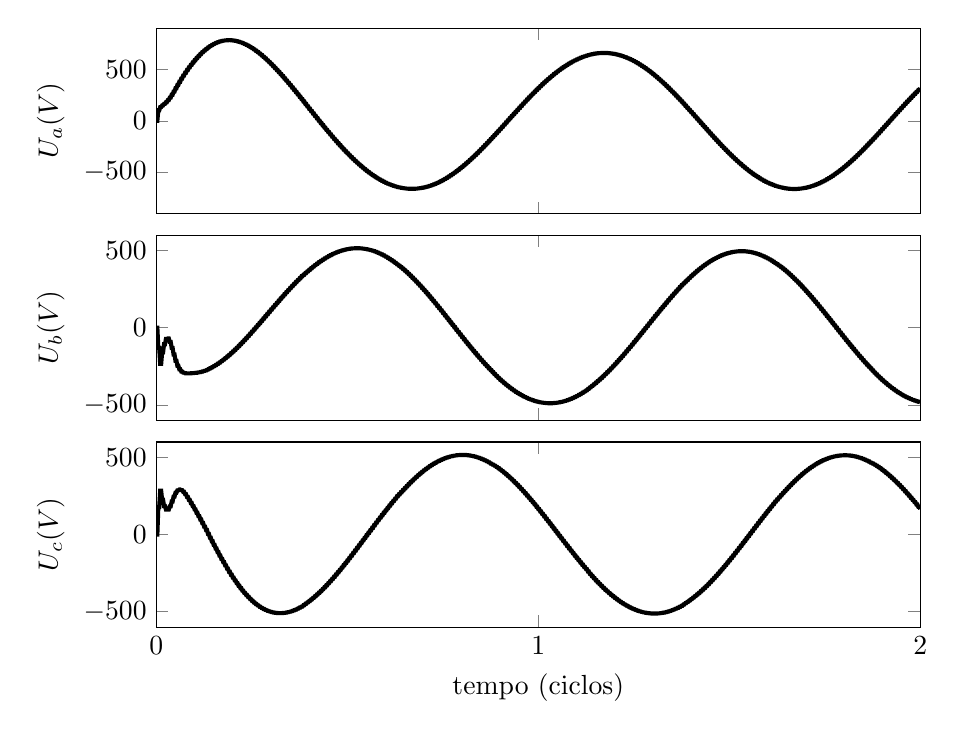
\begin{tikzpicture}

\begin{axis}[%
width=0.8\textwidth,
height=0.193917089240149\textwidth,
scale only axis,
xmin=0,
xmax=0.0333333333333333,
xtick={0,0.0166666666666667,0.0333333333333333},
xticklabels={\empty},
ymin=-600,
ymax=600,
ytick={-500,    0,  500},
ylabel={$\text{U}_\text{b}\text{ (V)}$},
name=plot2,
scaled x ticks = false,
legend columns=-1,
legend style={/tikz/every even column/.append style={column sep=0.3cm}},
legend style={font=\footnotesize}
]
\addplot [color=black,solid,line width=1.5pt,forget plot]
  table[row sep=crcr]{0	0\\
4.16666666666667e-05	0\\
8.33333333333333e-05	-131.208384981468\\
0.000125	-131.208384981468\\
0.000166666666666667	-234.584928965489\\
0.000208333333333333	-234.584928965489\\
0.00025	-160.168155779155\\
0.000291666666666667	-160.168155779155\\
0.000333333333333333	-107.543118489659\\
0.000375	-107.543118489659\\
0.000416666666666667	-73.888785936457\\
0.000458333333333333	-73.888785936457\\
0.0005	-69.7722509660634\\
0.000541666666666667	-69.7722509660634\\
0.000583333333333333	-92.1660340161349\\
0.000625	-92.1660340161349\\
0.000666666666666667	-130.752625769349\\
0.000708333333333333	-130.752625769349\\
0.00075	-174.324494279884\\
0.000791666666666667	-174.324494279884\\
0.000833333333333333	-214.442698151622\\
0.000875	-214.442698151622\\
0.000916666666666667	-246.509146338107\\
0.000958333333333333	-246.509146338107\\
0.001	-269.262100964021\\
0.00104166666666667	-269.262100964021\\
0.00108333333333333	-283.633370400021\\
0.001125	-283.633370400021\\
0.00116666666666667	-291.587806916656\\
0.00120833333333333	-291.587806916656\\
0.00125	-295.25032032309\\
0.00129166666666667	-295.25032032309\\
0.00133333333333333	-296.397867069654\\
0.001375	-296.397867069654\\
0.00141666666666667	-296.263907502466\\
0.00145833333333333	-296.263907502466\\
0.0015	-295.552582188269\\
0.00154166666666667	-295.552582188269\\
0.00158333333333333	-294.559622296515\\
0.001625	-294.559622296515\\
0.00166666666666667	-293.321890703225\\
0.00170833333333333	-293.321890703225\\
0.00175	-291.748630235435\\
0.00179166666666667	-291.748630235435\\
0.00183333333333333	-289.71441027203\\
0.001875	-289.71441027203\\
0.00191666666666667	-287.112155820289\\
0.00195833333333333	-287.112155820289\\
0.002	-283.874408274845\\
0.00204166666666667	-283.874408274845\\
0.00208333333333333	-279.974083042623\\
0.002125	-279.974083042623\\
0.00216666666666667	-276.230710645985\\
0.00220833333333333	-276.230710645985\\
0.00225	-269.902471427438\\
0.00229166666666667	-269.902471427438\\
0.00233333333333333	-263.390506882564\\
0.002375	-263.390506882564\\
0.00241666666666667	-256.603912012827\\
0.00245833333333333	-256.603912012827\\
0.0025	-249.467050045098\\
0.00254166666666667	-249.467050045098\\
0.00258333333333333	-241.924282867545\\
0.002625	-241.924282867545\\
0.00266666666666667	-233.943514769767\\
0.00270833333333333	-233.943514769767\\
0.00275	-225.51142526975\\
0.00279166666666667	-225.51142526975\\
0.00283333333333333	-216.627879066297\\
0.002875	-216.627879066297\\
0.00291666666666667	-207.301043117277\\
0.00295833333333333	-207.301043117277\\
0.003	-197.544304205697\\
0.00304166666666667	-197.544304205697\\
0.00308333333333333	-187.373993764868\\
0.003125	-187.373993764868\\
0.00316666666666667	-176.807799349931\\
0.00320833333333333	-176.807799349931\\
0.00325	-165.86394028825\\
0.00329166666666667	-165.86394028825\\
0.00333333333333333	-154.56053336183\\
0.003375	-154.56053336183\\
0.00341666666666667	-142.916185684556\\
0.00345833333333333	-142.916185684556\\
0.0035	-130.949486492199\\
0.00354166666666667	-130.949486492199\\
0.00358333333333333	-118.678959960814\\
0.003625	-118.678959960814\\
0.00366666666666667	-106.123619808363\\
0.00370833333333333	-106.123619808363\\
0.00375	-93.3030537323442\\
0.00379166666666667	-93.3030537323442\\
0.00383333333333333	-80.2372616130265\\
0.003875	-80.2372616130265\\
0.00391666666666667	-66.946446858932\\
0.00395833333333333	-66.946446858932\\
0.004	-53.4508475905557\\
0.00404166666666667	-53.4508475905557\\
0.00408333333333333	-39.7706293086077\\
0.004125	-39.7706293086077\\
0.00416666666666667	-25.9258298741469\\
0.00420833333333333	-25.9258298741469\\
0.00425	-11.9349140110245\\
0.00429166666666667	-11.9349140110245\\
0.00433333333333333	2.17790522937486\\
0.004375	2.17790522937486\\
0.00441666666666667	16.3962486462483\\
0.00445833333333333	16.3962486462483\\
0.0045	30.7006178618543\\
0.00454166666666667	30.7006178618543\\
0.00458333333333333	45.0716649106275\\
0.004625	45.0716649106275\\
0.00466666666666667	59.4905693391103\\
0.00470833333333333	59.4905693391103\\
0.00475	73.9392259321699\\
0.00479166666666667	73.9392259321699\\
0.00483333333333333	88.4001974163121\\
0.004875	88.4001974163121\\
0.00491666666666667	102.856536225067\\
0.00495833333333333	102.856536225067\\
0.005	117.29157109512\\
0.00504166666666667	117.29157109512\\
0.00508333333333333	131.688732283752\\
0.005125	131.688732283752\\
0.00516666666666667	146.031451752995\\
0.00520833333333333	146.031451752995\\
0.00525	160.303101705176\\
0.00529166666666667	160.303101705176\\
0.00533333333333333	174.487234885993\\
0.005375	174.487234885993\\
0.00541666666666667	188.567259559557\\
0.00545833333333333	188.567259559557\\
0.0055	202.526804768692\\
0.00554166666666667	202.526804768692\\
0.00558333333333333	216.349754514141\\
0.005625	216.349754514141\\
0.00566666666666667	230.020253035965\\
0.00570833333333333	230.020253035965\\
0.00575	243.522738831443\\
0.00579166666666667	243.522738831443\\
0.00583333333333333	256.84196321956\\
0.005875	256.84196321956\\
0.00591666666666667	269.962999410354\\
0.00595833333333333	269.962999410354\\
0.006	282.87124664738\\
0.00604166666666667	282.87124664738\\
0.00608333333333333	295.552432875164\\
0.006125	295.552432875164\\
0.00616666666666667	307.992617959481\\
0.00620833333333333	307.992617959481\\
0.00625	320.178198245509\\
0.00629166666666667	320.178198245509\\
0.00633333333333333	332.855329881327\\
0.006375	332.855329881327\\
0.00641666666666667	343.342330073383\\
0.00645833333333333	343.342330073383\\
0.0065	353.99049013455\\
0.00654166666666667	353.99049013455\\
0.00658333333333333	364.642135043666\\
0.006625	364.642135043666\\
0.00666666666666667	375.181419186422\\
0.00670833333333333	375.181419186422\\
0.00675	385.512898439921\\
0.00679166666666667	385.512898439921\\
0.00683333333333333	395.56751591175\\
0.006875	395.56751591175\\
0.00691666666666667	405.299190659419\\
0.00695833333333333	405.299190659419\\
0.007	414.6789771117\\
0.00704166666666667	414.6789771117\\
0.00708333333333333	423.689448232757\\
0.007125	423.689448232757\\
0.00716666666666667	432.319795582899\\
0.00720833333333333	432.319795582899\\
0.00725	440.562257768488\\
0.00729166666666667	440.562257768488\\
0.00733333333333333	448.410048149301\\
0.007375	448.410048149301\\
0.00741666666666667	455.855714179642\\
0.00745833333333333	455.855714179642\\
0.0075	462.892056329269\\
0.00754166666666667	462.892056329269\\
0.00758333333333333	469.511201648022\\
0.007625	469.511201648022\\
0.00766666666666667	475.705264661268\\
0.00770833333333333	475.705264661268\\
0.00775	481.466649529459\\
0.00779166666666667	481.466649529459\\
0.00783333333333333	486.78826836911\\
0.007875	486.78826836911\\
0.00791666666666667	491.663661719869\\
0.00795833333333333	491.663661719869\\
0.008	496.087037180632\\
0.00804166666666667	496.087037180632\\
0.00808333333333333	500.053254570176\\
0.008125	500.053254570176\\
0.00816666666666667	503.557785185404\\
0.00820833333333333	503.557785185404\\
0.00825	506.596665689598\\
0.00829166666666667	506.596665689598\\
0.00833333333333333	509.166458664863\\
0.008375	509.166458664863\\
0.00841666666666667	511.26284706523\\
0.00845833333333333	511.26284706523\\
0.0085	512.887878751787\\
0.00854166666666667	512.887878751787\\
0.00858333333333333	514.036243881462\\
0.008625	514.036243881462\\
0.00866666666666667	514.70657597084\\
0.00870833333333333	514.70657597084\\
0.00875	514.897900663887\\
0.00879166666666667	514.897900663887\\
0.00883333333333333	514.609349115043\\
0.008875	514.609349115043\\
0.00891666666666667	513.840063526413\\
0.00895833333333333	513.840063526413\\
0.009	512.589295351705\\
0.00904166666666667	512.589295351705\\
0.00908333333333333	510.856621488259\\
0.009125	510.856621488259\\
0.00916666666666667	508.642156970704\\
0.00920833333333333	508.642156970704\\
0.00925	505.94671097045\\
0.00929166666666667	505.94671097045\\
0.00933333333333333	502.771865436787\\
0.009375	502.771865436787\\
0.00941666666666667	499.120078655295\\
0.00945833333333333	499.120078655295\\
0.0095	494.994111068826\\
0.00954166666666667	494.994111068826\\
0.00958333333333333	490.398056463638\\
0.009625	490.398056463638\\
0.00966666666666667	485.336268084155\\
0.00970833333333333	485.336268084155\\
0.00975	479.813656395512\\
0.00979166666666667	479.813656395512\\
0.00983333333333333	473.835637893215\\
0.009875	473.835637893215\\
0.00991666666666667	467.40810543573\\
0.00995833333333333	467.40810543573\\
0.01	460.537409750096\\
0.0100416666666667	460.537409750096\\
0.0100833333333333	453.230348179938\\
0.010125	453.230348179938\\
0.0101666666666667	445.494156765893\\
0.0102083333333333	445.494156765893\\
0.01025	437.336502813829\\
0.0102916666666667	437.336502813829\\
0.0103333333333333	428.765476391161\\
0.010375	428.765476391161\\
0.0104166666666667	419.671168222686\\
0.0104583333333333	419.671168222686\\
0.0105	409.880726788609\\
0.0105416666666667	409.880726788609\\
0.0105833333333333	401.178503300298\\
0.010625	401.178503300298\\
0.0106666666666667	391.676757709522\\
0.0107083333333333	391.676757709522\\
0.01075	381.51592835396\\
0.0107916666666667	381.51592835396\\
0.0108333333333333	370.80234919461\\
0.010875	370.80234919461\\
0.0109166666666667	359.628279768278\\
0.0109583333333333	359.628279768278\\
0.011	348.062824063235\\
0.0110416666666667	348.062824063235\\
0.0110833333333333	336.152893739176\\
0.011125	336.152893739176\\
0.0111666666666667	323.928184426645\\
0.0112083333333333	323.928184426645\\
0.01125	311.407085810258\\
0.0112916666666667	311.407085810258\\
0.0113333333333333	298.601881290224\\
0.011375	298.601881290224\\
0.0114166666666667	285.522540449141\\
0.0114583333333333	285.522540449141\\
0.0115	272.178878667119\\
0.0115416666666667	272.178878667119\\
0.0115833333333333	258.582471388198\\
0.011625	258.582471388198\\
0.0116666666666667	244.745228379326\\
0.0117083333333333	244.745228379326\\
0.01175	230.680736573505\\
0.0117916666666667	230.680736573505\\
0.0118333333333333	216.403367701406\\
0.011875	216.403367701406\\
0.0119166666666667	201.927931320853\\
0.0119583333333333	201.927931320853\\
0.012	187.269408777014\\
0.0120416666666667	187.269408777014\\
0.0120833333333333	172.442797815245\\
0.012125	172.442797815245\\
0.0121666666666667	157.46304906022\\
0.0122083333333333	157.46304906022\\
0.01225	142.345062821324\\
0.0122916666666667	142.345062821324\\
0.0123333333333333	127.103715658411\\
0.012375	127.103715658411\\
0.0124166666666667	111.753893917898\\
0.0124583333333333	111.753893917898\\
0.0125	96.3112704188052\\
0.0125416666666667	96.3112704188052\\
0.0125833333333333	80.7890128332204\\
0.012625	80.7890128332204\\
0.0126666666666667	65.2021424948018\\
0.0127083333333333	65.2021424948018\\
0.01275	49.5668545196005\\
0.0127916666666667	49.5668545196005\\
0.0128333333333333	33.8981375093313\\
0.012875	33.8981375093313\\
0.0129166666666667	18.2111944355166\\
0.0129583333333333	18.2111944355166\\
0.013	2.52164301433743\\
0.0130416666666667	2.52164301433743\\
0.0130833333333333	-13.1544965438618\\
0.013125	-13.1544965438618\\
0.0131666666666667	-28.8009586278613\\
0.0132083333333333	-28.8009586278613\\
0.01325	-44.4014501836413\\
0.0132916666666667	-44.4014501836413\\
0.0133333333333333	-59.9398537968807\\
0.013375	-59.9398537968807\\
0.0134166666666667	-75.4003693774317\\
0.0134583333333333	-75.4003693774317\\
0.0135	-90.7675815462738\\
0.0135416666666667	-90.7675815462738\\
0.0135833333333333	-106.026592391776\\
0.013625	-106.026592391776\\
0.0136666666666667	-121.162260382374\\
0.0137083333333333	-121.162260382374\\
0.01375	-136.160662302134\\
0.0137916666666667	-136.160662302134\\
0.0138333333333333	-151.007656217058\\
0.013875	-151.007656217058\\
0.0139166666666667	-165.689332400057\\
0.0139583333333333	-165.689332400057\\
0.014	-180.191986276356\\
0.0140416666666667	-180.191986276356\\
0.0140833333333333	-194.502113222519\\
0.014125	-194.502113222519\\
0.0141666666666667	-208.606411769966\\
0.0142083333333333	-208.606411769966\\
0.01425	-222.491792056468\\
0.0142916666666667	-222.491792056468\\
0.0143333333333333	-236.145386407417\\
0.014375	-236.145386407417\\
0.0144166666666667	-249.554559936585\\
0.0144583333333333	-249.554559936585\\
0.0145	-262.706920156191\\
0.0145416666666667	-262.706920156191\\
0.0145833333333333	-274.897866458395\\
0.014625	-274.897866458395\\
0.0146666666666667	-288.422767271497\\
0.0147083333333333	-288.422767271497\\
0.01475	-301.387581541166\\
0.0147916666666667	-301.387581541166\\
0.0148333333333333	-313.775025011641\\
0.014875	-313.775025011641\\
0.0149166666666667	-325.666355207773\\
0.0149583333333333	-325.666355207773\\
0.015	-337.120887117542\\
0.0150416666666667	-337.120887117542\\
0.0150833333333333	-348.176422957511\\
0.015125	-348.176422957511\\
0.0151666666666667	-358.852722723377\\
0.0152083333333333	-358.852722723377\\
0.01525	-369.156522014211\\
0.0152916666666667	-369.156522014211\\
0.0153333333333333	-379.086218179142\\
0.015375	-379.086218179142\\
0.0154166666666667	-388.635603200765\\
0.0154583333333333	-388.635603200765\\
0.0155	-397.796477626206\\
0.0155416666666667	-397.796477626206\\
0.0155833333333333	-406.560220436797\\
0.015625	-406.560220436797\\
0.0156666666666667	-414.918572567047\\
0.0157083333333333	-414.918572567047\\
0.01575	-422.864533448988\\
0.0157916666666667	-422.864533448988\\
0.0158333333333333	-430.390775276099\\
0.015875	-430.390775276099\\
0.0159166666666667	-437.491100853172\\
0.0159583333333333	-437.491100853172\\
0.016	-444.159730520883\\
0.0160416666666667	-444.159730520883\\
0.0160833333333333	-450.391206601553\\
0.016125	-450.391206601553\\
0.0161666666666667	-456.180340052471\\
0.0162083333333333	-456.180340052471\\
0.01625	-461.522202906791\\
0.0162916666666667	-461.522202906791\\
0.0163333333333333	-466.412149544966\\
0.016375	-466.412149544966\\
0.0164166666666667	-470.845850821675\\
0.0164583333333333	-470.845850821675\\
0.0165	-474.819329326491\\
0.0165416666666667	-474.819329326491\\
0.0165833333333333	-478.328989103039\\
0.016625	-478.328989103039\\
0.0166666666666667	-481.372762295986\\
0.0167083333333333	-481.372762295986\\
0.01675	-483.944387417357\\
0.0167916666666667	-483.944387417357\\
0.0168333333333333	-486.043904769891\\
0.016875	-486.043904769891\\
0.0169166666666667	-487.669342075457\\
0.0169583333333333	-487.669342075457\\
0.017	-488.81912329053\\
0.0170416666666667	-488.81912329053\\
0.0170833333333333	-489.492376222951\\
0.017125	-489.492376222951\\
0.0171666666666667	-489.689089295181\\
0.0172083333333333	-489.689089295181\\
0.01725	-489.410057478733\\
0.0172916666666667	-489.410057478733\\
0.0173333333333333	-488.656714544629\\
0.017375	-488.656714544629\\
0.0174166666666667	-487.430933830334\\
0.0174583333333333	-487.430933830334\\
0.0175	-485.734862735459\\
0.0175416666666667	-485.734862735459\\
0.0175833333333333	-483.570824107468\\
0.017625	-483.570824107468\\
0.0176666666666667	-480.941176730971\\
0.0177083333333333	-480.941176730971\\
0.01775	-477.848873406491\\
0.0177916666666667	-477.848873406491\\
0.0178333333333333	-474.296687037085\\
0.017875	-474.296687037085\\
0.0179166666666667	-470.287554266504\\
0.0179583333333333	-470.287554266504\\
0.018	-465.824994538518\\
0.0180416666666667	-465.824994538518\\
0.0180833333333333	-460.912896166831\\
0.018125	-460.912896166831\\
0.0181666666666667	-455.555544349316\\
0.0182083333333333	-455.555544349316\\
0.01825	-449.757632700212\\
0.0182916666666667	-449.757632700212\\
0.0183333333333333	-443.524266807923\\
0.018375	-443.524266807923\\
0.0184166666666667	-436.860963041735\\
0.0184583333333333	-436.860963041735\\
0.0185	-429.773645406549\\
0.0185416666666667	-429.773645406549\\
0.0185833333333333	-422.2686421737\\
0.018625	-422.2686421737\\
0.0186666666666667	-414.352682994809\\
0.0187083333333333	-414.352682994809\\
0.01875	-406.710604021129\\
0.0187916666666667	-406.710604021129\\
0.0188333333333333	-396.968651829484\\
0.018875	-396.968651829484\\
0.0189166666666667	-387.24430030011\\
0.0189583333333333	-387.24430030011\\
0.019	-377.413842111121\\
0.0190416666666667	-377.413842111121\\
0.0190833333333333	-367.3960735467\\
0.019125	-367.3960735467\\
0.0191666666666667	-357.12553953726\\
0.0192083333333333	-357.12553953726\\
0.01925	-346.559303382721\\
0.0192916666666667	-346.559303382721\\
0.0193333333333333	-335.674936708767\\
0.019375	-335.674936708767\\
0.0194166666666667	-324.465686057335\\
0.0194583333333333	-324.465686057335\\
0.0195	-312.935239244225\\
0.0195416666666667	-312.935239244225\\
0.0195833333333333	-301.093266862382\\
0.019625	-301.093266862382\\
0.0196666666666667	-288.95219973374\\
0.0197083333333333	-288.95219973374\\
0.01975	-276.525463982029\\
0.0197916666666667	-276.525463982029\\
0.0198333333333333	-263.82538033546\\
0.019875	-263.82538033546\\
0.0199166666666667	-250.865057706918\\
0.0199583333333333	-250.865057706918\\
0.02	-237.656697428642\\
0.0200416666666667	-237.656697428642\\
0.0200833333333333	-224.212271375033\\
0.020125	-224.212271375033\\
0.0201666666666667	-210.543848998092\\
0.0202083333333333	-210.543848998092\\
0.02025	-196.6637735981\\
0.0202916666666667	-196.6637735981\\
0.0203333333333333	-182.584756063204\\
0.020375	-182.584756063204\\
0.0204166666666667	-168.319897946886\\
0.0204583333333333	-168.319897946886\\
0.0205	-153.882668002172\\
0.0205416666666667	-153.882668002172\\
0.0205833333333333	-139.286855686717\\
0.020625	-139.286855686717\\
0.0206666666666667	-124.546519243168\\
0.0207083333333333	-124.546519243168\\
0.02075	-109.675923407492\\
0.0207916666666667	-109.675923407492\\
0.0208333333333333	-94.6884951690301\\
0.020875	-94.6884951690301\\
0.0209166666666667	-79.6023211852309\\
0.0209583333333333	-79.6023211852309\\
0.021	-64.4296541414652\\
0.0210416666666667	-64.4296541414652\\
0.0210833333333333	-49.1854677870168\\
0.021125	-49.1854677870168\\
0.0211666666666667	-33.8847697005379\\
0.0212083333333333	-33.8847697005379\\
0.02125	-18.5423320716325\\
0.0212916666666667	-18.5423320716325\\
0.0213333333333333	-3.1725945533516\\
0.021375	-3.1725945533516\\
0.0214166666666667	12.2102617721841\\
0.0214583333333333	12.2102617721841\\
0.0215	27.5921432856442\\
0.0215416666666667	27.5921432856442\\
0.0215833333333333	42.9588704890498\\
0.021625	42.9588704890498\\
0.0216666666666667	58.2960537853681\\
0.0217083333333333	58.2960537853681\\
0.02175	73.5890384864759\\
0.0217916666666667	73.5890384864759\\
0.0218333333333333	88.82269659409\\
0.021875	88.82269659409\\
0.0219166666666667	103.982669291038\\
0.0219583333333333	103.982669291038\\
0.022	119.053037141893\\
0.0220416666666667	119.053037141893\\
0.0220833333333333	134.01853586672\\
0.022125	134.01853586672\\
0.0221666666666667	148.863909368128\\
0.0222083333333333	148.863909368128\\
0.02225	163.573956427556\\
0.0222916666666667	163.573956427556\\
0.0223333333333333	178.133568427636\\
0.022375	178.133568427636\\
0.0224166666666667	192.527757716713\\
0.0224583333333333	192.527757716713\\
0.0225	206.741679404245\\
0.0225416666666667	206.741679404245\\
0.0225833333333333	220.760649670751\\
0.022625	220.760649670751\\
0.0226666666666667	234.570162946369\\
0.0227083333333333	234.570162946369\\
0.02275	248.155909263895\\
0.0227916666666667	248.155909263895\\
0.0228333333333333	261.687830320942\\
0.022875	261.687830320942\\
0.0229166666666667	274.986604079196\\
0.0229583333333333	274.986604079196\\
0.023	286.928801747272\\
0.0230416666666667	286.928801747272\\
0.0230833333333333	298.950506950644\\
0.023125	298.950506950644\\
0.0231666666666667	310.924864102034\\
0.0232083333333333	310.924864102034\\
0.02325	322.756989832147\\
0.0232916666666667	322.756989832147\\
0.0233333333333333	334.367084014297\\
0.023375	334.367084014297\\
0.0234166666666667	345.69602196514\\
0.0234583333333333	345.69602196514\\
0.0235	356.703461032175\\
0.0235416666666667	356.703461032175\\
0.0235833333333333	367.363371170442\\
0.023625	367.363371170442\\
0.0236666666666667	377.659204280424\\
0.0237083333333333	377.659204280424\\
0.02375	387.579795487262\\
0.0237916666666667	387.579795487262\\
0.0238333333333333	397.116425283701\\
0.023875	397.116425283701\\
0.0239166666666667	406.261310362139\\
0.0239583333333333	406.261310362139\\
0.024	415.0053223807\\
0.0240416666666667	415.0053223807\\
0.0240833333333333	423.340732147141\\
0.024125	423.340732147141\\
0.0241666666666667	431.258683016742\\
0.0242083333333333	431.258683016742\\
0.02425	438.750365395371\\
0.0242916666666667	438.750365395371\\
0.0243333333333333	445.807262831054\\
0.024375	445.807262831054\\
0.0244166666666667	452.421342397773\\
0.0244583333333333	452.421342397773\\
0.0245	458.585161293933\\
0.0245416666666667	458.585161293933\\
0.0245833333333333	464.291905294308\\
0.024625	464.291905294308\\
0.0246666666666667	469.535383109734\\
0.0247083333333333	469.535383109734\\
0.02475	474.309999446141\\
0.0247916666666667	474.309999446141\\
0.0248333333333333	478.610723480444\\
0.024875	478.610723480444\\
0.0249166666666667	482.432523836755\\
0.0249583333333333	482.432523836755\\
0.025	485.772612186125\\
0.0250416666666667	485.772612186125\\
0.0250833333333333	488.627883686145\\
0.025125	488.627883686145\\
0.0251666666666667	490.994391489966\\
0.0252083333333333	490.994391489966\\
0.02525	492.869784189106\\
0.0252916666666667	492.869784189106\\
0.0253333333333333	494.252063559781\\
0.025375	494.252063559781\\
0.0254166666666667	495.139387583695\\
0.0254583333333333	495.139387583695\\
0.0255	495.530061759552\\
0.0255416666666667	495.530061759552\\
0.0255833333333333	495.422663936061\\
0.025625	495.422663936061\\
0.0256666666666667	494.816230581684\\
0.0257083333333333	494.816230581684\\
0.02575	493.710425995119\\
0.0257916666666667	493.710425995119\\
0.0258333333333333	492.105654148384\\
0.025875	492.105654148384\\
0.0259166666666667	490.003108134894\\
0.0259583333333333	490.003108134894\\
0.026	487.404961487327\\
0.0260416666666667	487.404961487327\\
0.0260833333333333	484.313069214194\\
0.026125	484.313069214194\\
0.0261666666666667	480.731558886196\\
0.0262083333333333	480.731558886196\\
0.02625	476.664323712434\\
0.0262916666666667	476.664323712434\\
0.0263333333333333	472.115829454631\\
0.026375	472.115829454631\\
0.0264166666666667	467.091068733291\\
0.0264583333333333	467.091068733291\\
0.0265	461.595540479995\\
0.0265416666666667	461.595540479995\\
0.0265833333333333	455.635234907076\\
0.026625	455.635234907076\\
0.0266666666666667	449.21662231492\\
0.0267083333333333	449.21662231492\\
0.02675	442.346643428456\\
0.0267916666666667	442.346643428456\\
0.0268333333333333	435.032699614098\\
0.026875	435.032699614098\\
0.0269166666666667	427.282642172915\\
0.0269583333333333	427.282642172915\\
0.027	418.527982244731\\
0.0270416666666667	418.527982244731\\
0.0270833333333333	410.672570182659\\
0.027125	410.672570182659\\
0.0271666666666667	402.276872290978\\
0.0272083333333333	402.276872290978\\
0.02725	393.223850223727\\
0.0272916666666667	393.223850223727\\
0.0273333333333333	383.609151155178\\
0.027375	383.609151155178\\
0.0274166666666667	373.508718653929\\
0.0274583333333333	373.508718653929\\
0.0275	362.979579538073\\
0.0275416666666667	362.979579538073\\
0.0275833333333333	352.061894709897\\
0.027625	352.061894709897\\
0.0276666666666667	340.783205444461\\
0.0277083333333333	340.783205444461\\
0.02775	329.162781541968\\
0.0277916666666667	329.162781541968\\
0.0278333333333333	317.215226351439\\
0.027875	317.215226351439\\
0.0279166666666667	304.953068995059\\
0.0279583333333333	304.953068995059\\
0.028	292.388308765939\\
0.0280416666666667	292.388308765939\\
0.0280833333333333	279.533394256386\\
0.028125	279.533394256386\\
0.0281666666666667	266.401997020689\\
0.0282083333333333	266.401997020689\\
0.02825	253.007121767018\\
0.0282916666666667	253.007121767018\\
0.0283333333333333	239.363037342399\\
0.028375	239.363037342399\\
0.0284166666666667	225.484309796947\\
0.0284583333333333	225.484309796947\\
0.0285	211.385672071801\\
0.0285416666666667	211.385672071801\\
0.0285833333333333	197.081935254737\\
0.028625	197.081935254737\\
0.0286666666666667	182.587950486431\\
0.0287083333333333	182.587950486431\\
0.02875	167.918604082923\\
0.0287916666666667	167.918604082923\\
0.0288333333333333	153.088829011011\\
0.028875	153.088829011011\\
0.0289166666666667	138.113619934855\\
0.0289583333333333	138.113619934855\\
0.029	123.008044204917\\
0.0290416666666667	123.008044204917\\
0.0290833333333333	107.788100944899\\
0.029125	107.788100944899\\
0.0291666666666667	92.4664220892656\\
0.0292083333333333	92.4664220892656\\
0.02925	77.0599110293703\\
0.0292916666666667	77.0599110293703\\
0.0293333333333333	61.5839402726698\\
0.029375	61.5839402726698\\
0.0294166666666667	46.0538191073489\\
0.0294583333333333	46.0538191073489\\
0.0295	30.4851141949034\\
0.0295416666666667	30.4851141949034\\
0.0295833333333333	14.8937682112207\\
0.029625	14.8937682112207\\
0.0296666666666667	-0.703957306529608\\
0.0297083333333333	-0.703957306529608\\
0.02975	-16.2916492298269\\
0.0297916666666667	-16.2916492298269\\
0.0298333333333333	-31.8529362123827\\
0.029875	-31.8529362123827\\
0.0299166666666667	-47.371649369948\\
0.0299583333333333	-47.371649369948\\
0.03	-62.8319222299047\\
0.0300416666666667	-62.8319222299047\\
0.0300833333333333	-78.2183969102601\\
0.030125	-78.2183969102601\\
0.0301666666666667	-93.5154108314719\\
0.0302083333333333	-93.5154108314719\\
0.03025	-108.70816278091\\
0.0302916666666667	-108.70816278091\\
0.0303333333333333	-123.782356080195\\
0.030375	-123.782356080195\\
0.0304166666666667	-138.723507249364\\
0.0304583333333333	-138.723507249364\\
0.0305	-153.517339096442\\
0.0305416666666667	-153.517339096442\\
0.0305833333333333	-168.149764544084\\
0.030625	-168.149764544084\\
0.0306666666666667	-182.60688669631\\
0.0307083333333333	-182.60688669631\\
0.03075	-196.875004412733\\
0.0307916666666667	-196.875004412733\\
0.0308333333333333	-210.940621254231\\
0.030875	-210.940621254231\\
0.0309166666666667	-224.790455634942\\
0.0309583333333333	-224.790455634942\\
0.031	-238.411450801645\\
0.0310416666666667	-238.411450801645\\
0.0310833333333333	-251.788204920739\\
0.031125	-251.788204920739\\
0.0311666666666667	-264.319493294975\\
0.0312083333333333	-264.319493294975\\
0.03125	-278.081845363642\\
0.0312916666666667	-278.081845363642\\
0.0313333333333333	-291.211888263673\\
0.031375	-291.211888263673\\
0.0314166666666667	-303.807007713181\\
0.0314583333333333	-303.807007713181\\
0.0315	-315.936364357588\\
0.0315416666666667	-315.936364357588\\
0.0315833333333333	-327.655020751537\\
0.031625	-327.655020751537\\
0.0316666666666667	-338.998550237152\\
0.0317083333333333	-338.998550237152\\
0.03175	-349.984949605885\\
0.0317916666666667	-349.984949605885\\
0.0318333333333333	-360.618974262017\\
0.031875	-360.618974262017\\
0.0319166666666667	-370.896795074955\\
0.0319583333333333	-370.896795074955\\
0.032	-380.809923421548\\
0.0320416666666667	-380.809923421548\\
0.0320833333333333	-390.348041070204\\
0.032125	-390.348041070204\\
0.0321666666666667	-399.500455565927\\
0.0322083333333333	-399.500455565927\\
0.03225	-408.258433783543\\
0.0322916666666667	-408.258433783543\\
0.0323333333333333	-416.612673979994\\
0.032375	-416.612673979994\\
0.0324166666666667	-424.555376388038\\
0.0324583333333333	-424.555376388038\\
0.0325	-432.079651399668\\
0.0325416666666667	-432.079651399668\\
0.0325833333333333	-439.17912856472\\
0.032625	-439.17912856472\\
0.0326666666666667	-445.847803165625\\
0.0327083333333333	-445.847803165625\\
0.03275	-452.079952433882\\
0.0327916666666667	-452.079952433882\\
0.0328333333333333	-457.870112681898\\
0.032875	-457.870112681898\\
0.0329166666666667	-463.213095942823\\
0.0329583333333333	-463.213095942823\\
0.033	-468.104025539882\\
0.0330416666666667	-468.104025539882\\
0.0330833333333333	-472.538375275198\\
0.033125	-472.538375275198\\
0.0331666666666667	-476.512043591712\\
0.0332083333333333	-476.512043591712\\
0.03325	-480.021998518076\\
0.0332916666666667	-480.021998518076\\
0.0333333333333333	-483.062409528906\\
};
\end{axis}

\begin{axis}[%
width=0.8\textwidth,
height=0.193917089240149\textwidth,
scale only axis,
xmin=0,
xmax=0.0333333333333333,
xtick={0,0.0166666666666667,0.0333333333333333},
xticklabels={{0},{1},{2}},
xlabel={tempo (ciclos)},
ymin=-600,
ymax=600,
ytick={-500,    0,  500},
ylabel={$\text{U}_\text{c}\text{ (V)}$},
at=(plot2.below south west),
anchor=above north west,
scaled x ticks = false,
legend columns=-1,
legend style={/tikz/every even column/.append style={column sep=0.3cm}},
legend style={font=\footnotesize}
]
\addplot [color=black,solid,line width=1.5pt,forget plot]
  table[row sep=crcr]{0	0\\
4.16666666666667e-05	0\\
8.33333333333333e-05	178.004625595273\\
0.000125	178.004625595273\\
0.000166666666666667	283.783478314647\\
0.000208333333333333	283.783478314647\\
0.00025	224.921982240448\\
0.000291666666666667	224.921982240448\\
0.000333333333333333	184.950751047334\\
0.000375	184.950751047334\\
0.000416666666666667	161.297963182983\\
0.000458333333333333	161.297963182983\\
0.0005	161.820809180068\\
0.000541666666666667	161.820809180068\\
0.000583333333333333	182.600021490024\\
0.000625	182.600021490024\\
0.000666666666666667	213.852580818456\\
0.000708333333333333	213.852580818456\\
0.00075	245.650747681198\\
0.000791666666666667	245.650747681198\\
0.000833333333333333	270.969555601234\\
0.000875	270.969555601234\\
0.000916666666666667	286.39849397629\\
0.000958333333333333	286.39849397629\\
0.001	291.501650773087\\
0.00104166666666667	291.501650773087\\
0.00108333333333333	287.689293494019\\
0.001125	287.689293494019\\
0.00116666666666667	277.144952722096\\
0.00120833333333333	277.144952722096\\
0.00125	262.056791666573\\
0.00129166666666667	262.056791666573\\
0.00133333333333333	244.197984718012\\
0.001375	244.197984718012\\
0.00141666666666667	224.790878827205\\
0.00145833333333333	224.790878827205\\
0.0015	204.552290090145\\
0.00154166666666667	204.552290090145\\
0.00158333333333333	183.823710668467\\
0.001625	183.823710668467\\
0.00166666666666667	162.716831956078\\
0.00170833333333333	162.716831956078\\
0.00175	141.234887842283\\
0.00179166666666667	141.234887842283\\
0.00183333333333333	119.35496285977\\
0.001875	119.35496285977\\
0.00191666666666667	97.0724508524626\\
0.00195833333333333	97.0724508524626\\
0.002	74.4167689879326\\
0.00204166666666667	74.4167689879326\\
0.00208333333333333	51.4493873847393\\
0.002125	51.4493873847393\\
0.00216666666666667	29.3933134371395\\
0.00220833333333333	29.3933134371395\\
0.00225	4.5154200136966\\
0.00229166666666667	4.5154200136966\\
0.00233333333333333	-19.8430703521883\\
0.002375	-19.8430703521883\\
0.00241666666666667	-43.7452284674193\\
0.00245833333333333	-43.7452284674193\\
0.0025	-67.2437290269028\\
0.00254166666666667	-67.2437290269028\\
0.00258333333333333	-90.374341557218\\
0.002625	-90.374341557218\\
0.00266666666666667	-113.147583195981\\
0.00270833333333333	-113.147583195981\\
0.00275	-135.552273116364\\
0.00279166666666667	-135.552273116364\\
0.00283333333333333	-157.561983919016\\
0.002875	-157.561983919016\\
0.00291666666666667	-179.14154545017\\
0.00295833333333333	-179.14154545017\\
0.003	-200.251748337301\\
0.00304166666666667	-200.251748337301\\
0.00308333333333333	-220.852877551901\\
0.003125	-220.852877551901\\
0.00316666666666667	-240.907089135164\\
0.00320833333333333	-240.907089135164\\
0.00325	-260.379576837184\\
0.00329166666666667	-260.379576837184\\
0.00333333333333333	-279.239350290979\\
0.003375	-279.239350290979\\
0.00341666666666667	-297.458284795409\\
0.00345833333333333	-297.458284795409\\
0.0035	-315.011576336968\\
0.00354166666666667	-315.011576336968\\
0.00358333333333333	-331.876739706872\\
0.003625	-331.876739706872\\
0.00366666666666667	-348.033836396141\\
0.00370833333333333	-348.033836396141\\
0.00375	-363.465376357984\\
0.00379166666666667	-363.465376357984\\
0.00383333333333333	-378.156103365302\\
0.003875	-378.156103365302\\
0.00391666666666667	-392.092812734721\\
0.00395833333333333	-392.092812734721\\
0.004	-405.264238535789\\
0.00404166666666667	-405.264238535789\\
0.00408333333333333	-417.66099575086\\
0.004125	-417.66099575086\\
0.00416666666666667	-429.275548297076\\
0.00420833333333333	-429.275548297076\\
0.00425	-440.102848900291\\
0.00429166666666667	-440.102848900291\\
0.00433333333333333	-450.136815525274\\
0.004375	-450.136815525274\\
0.00441666666666667	-459.376722037127\\
0.00445833333333333	-459.376722037127\\
0.0045	-467.821856969954\\
0.00454166666666667	-467.821856969954\\
0.00458333333333333	-475.473032640935\\
0.004625	-475.473032640935\\
0.00466666666666667	-482.332742676867\\
0.00470833333333333	-482.332742676867\\
0.00475	-488.405171398126\\
0.00479166666666667	-488.405171398126\\
0.00483333333333333	-493.696011215487\\
0.004875	-493.696011215487\\
0.00491666666666667	-498.212188101641\\
0.00495833333333333	-498.212188101641\\
0.005	-501.961580121402\\
0.00504166666666667	-501.961580121402\\
0.00508333333333333	-504.952789601296\\
0.005125	-504.952789601296\\
0.00516666666666667	-507.194994417279\\
0.00520833333333333	-507.194994417279\\
0.00525	-508.697818385253\\
0.00529166666666667	-508.697818385253\\
0.00533333333333333	-509.471593317843\\
0.005375	-509.471593317843\\
0.00541666666666667	-509.526863255645\\
0.00545833333333333	-509.526863255645\\
0.0055	-508.874727992641\\
0.00554166666666667	-508.874727992641\\
0.00558333333333333	-507.526855287823\\
0.005625	-507.526855287823\\
0.00566666666666667	-505.495407493961\\
0.00570833333333333	-505.495407493961\\
0.00575	-502.793024217572\\
0.00579166666666667	-502.793024217572\\
0.00583333333333333	-499.432794031877\\
0.005875	-499.432794031877\\
0.00591666666666667	-495.428221057553\\
0.00595833333333333	-495.428221057553\\
0.006	-490.793190368868\\
0.00604166666666667	-490.793190368868\\
0.00608333333333333	-485.54193498711\\
0.006125	-485.54193498711\\
0.00616666666666667	-479.689005886904\\
0.00620833333333333	-479.689005886904\\
0.00625	-473.249245351608\\
0.00629166666666667	-473.249245351608\\
0.00633333333333333	-467.298164949134\\
0.006375	-467.298164949134\\
0.00641666666666667	-458.147227910362\\
0.00645833333333333	-458.147227910362\\
0.0065	-449.066214705222\\
0.00654166666666667	-449.066214705222\\
0.00658333333333333	-439.891191771422\\
0.006625	-439.891191771422\\
0.00666666666666667	-430.495153433043\\
0.00670833333333333	-430.495153433043\\
0.00675	-420.77695941029\\
0.00679166666666667	-420.77695941029\\
0.00683333333333333	-410.670766826443\\
0.006875	-410.670766826443\\
0.00691666666666667	-400.142827213577\\
0.00695833333333333	-400.142827213577\\
0.007	-389.183812623598\\
0.00704166666666667	-389.183812623598\\
0.00708333333333333	-377.800189443289\\
0.007125	-377.800189443289\\
0.00716666666666667	-366.007139201097\\
0.00720833333333333	-366.007139201097\\
0.00725	-353.823562705966\\
0.00729166666666667	-353.823562705966\\
0.00733333333333333	-341.269218925638\\
0.007375	-341.269218925638\\
0.00741666666666667	-328.362469641968\\
0.00745833333333333	-328.362469641968\\
0.0075	-315.121481823484\\
0.00754166666666667	-315.121481823484\\
0.00758333333333333	-301.562947743627\\
0.007625	-301.562947743627\\
0.00766666666666667	-287.70292901112\\
0.00770833333333333	-287.70292901112\\
0.00775	-273.557232892287\\
0.00779166666666667	-273.557232892287\\
0.00783333333333333	-259.141683855914\\
0.007875	-259.141683855914\\
0.00791666666666667	-244.472273340152\\
0.00795833333333333	-244.472273340152\\
0.008	-229.565207512913\\
0.00804166666666667	-229.565207512913\\
0.00808333333333333	-214.436888539275\\
0.008125	-214.436888539275\\
0.00816666666666667	-199.103863773767\\
0.00820833333333333	-199.103863773767\\
0.00825	-183.582768321516\\
0.00829166666666667	-183.582768321516\\
0.00833333333333333	-167.890275701312\\
0.008375	-167.890275701312\\
0.00841666666666667	-152.04244733988\\
0.00845833333333333	-152.04244733988\\
0.0085	-136.05795452593\\
0.00854166666666667	-136.05795452593\\
0.00858333333333333	-119.951965514414\\
0.008625	-119.951965514414\\
0.00866666666666667	-103.741190475133\\
0.00870833333333333	-103.741190475133\\
0.00875	-87.4422091632389\\
0.00879166666666667	-87.4422091632389\\
0.00883333333333333	-71.0712701286369\\
0.008875	-71.0712701286369\\
0.00891666666666667	-54.6442399391995\\
0.00895833333333333	-54.6442399391995\\
0.009	-38.176713696354\\
0.00904166666666667	-38.176713696354\\
0.00908333333333333	-21.6841757169129\\
0.009125	-21.6841757169129\\
0.00916666666666667	-5.18216699897625\\
0.00920833333333333	-5.18216699897625\\
0.00925	11.3135983475548\\
0.00929166666666667	11.3135983475548\\
0.00933333333333333	27.7871882840866\\
0.009375	27.7871882840866\\
0.00941666666666667	44.2223308532296\\
0.00945833333333333	44.2223308532296\\
0.0095	60.6032444540017\\
0.00954166666666667	60.6032444540017\\
0.00958333333333333	76.9131639720522\\
0.009625	76.9131639720522\\
0.00966666666666667	93.1358067368588\\
0.00970833333333333	93.1358067368588\\
0.00975	109.254960007813\\
0.00979166666666667	109.254960007813\\
0.00983333333333333	125.254535256242\\
0.009875	125.254535256242\\
0.00991666666666667	141.118601346748\\
0.00995833333333333	141.118601346748\\
0.01	156.83140708878\\
0.0100416666666667	156.83140708878\\
0.0100833333333333	172.377396967822\\
0.010125	172.377396967822\\
0.0101666666666667	187.741223638366\\
0.0102083333333333	187.741223638366\\
0.01025	202.907759665792\\
0.0102916666666667	202.907759665792\\
0.0103333333333333	217.862109793741\\
0.010375	217.862109793741\\
0.0104166666666667	232.754774400292\\
0.0104583333333333	232.754774400292\\
0.0105	247.828611366131\\
0.0105416666666667	247.828611366131\\
0.0105833333333333	260.603260690465\\
0.010625	260.603260690465\\
0.0106666666666667	273.680687269622\\
0.0107083333333333	273.680687269622\\
0.01075	286.883764607617\\
0.0107916666666667	286.883764607617\\
0.0108333333333333	300.065387824424\\
0.010875	300.065387824424\\
0.0109166666666667	313.098555619261\\
0.0109583333333333	313.098555619261\\
0.011	325.889085035844\\
0.0110416666666667	325.889085035844\\
0.0110833333333333	338.374638010692\\
0.011125	338.374638010692\\
0.0111666666666667	350.517946768375\\
0.0112083333333333	350.517946768375\\
0.01125	362.298555343427\\
0.0112916666666667	362.298555343427\\
0.0113333333333333	373.705464682803\\
0.011375	373.705464682803\\
0.0114166666666667	384.731726726044\\
0.0114583333333333	384.731726726044\\
0.0115	395.371336948598\\
0.0115416666666667	395.371336948598\\
0.0115833333333333	405.616529484539\\
0.011625	405.616529484539\\
0.0116666666666667	415.459679980571\\
0.0117083333333333	415.459679980571\\
0.01175	424.891495449277\\
0.0117916666666667	424.891495449277\\
0.0118333333333333	433.902229575715\\
0.011875	433.902229575715\\
0.0119166666666667	442.482176818538\\
0.0119583333333333	442.482176818538\\
0.012	450.622046686112\\
0.0120416666666667	450.622046686112\\
0.0120833333333333	458.313179351795\\
0.012125	458.313179351795\\
0.0121666666666667	465.547628342919\\
0.0122083333333333	465.547628342919\\
0.01225	472.31815507542\\
0.0122916666666667	472.31815507542\\
0.0123333333333333	478.618179027316\\
0.012375	478.618179027316\\
0.0124166666666667	484.441716434643\\
0.0124583333333333	484.441716434643\\
0.0125	489.783056377473\\
0.0125416666666667	489.783056377473\\
0.0125833333333333	494.63785268411\\
0.012625	494.63785268411\\
0.0126666666666667	499.001883658817\\
0.0127083333333333	499.001883658817\\
0.01275	502.870683009938\\
0.0127916666666667	502.870683009938\\
0.0128333333333333	506.240849585294\\
0.012875	506.240849585294\\
0.0129166666666667	509.109305926703\\
0.0129583333333333	509.109305926703\\
0.013	511.473151542652\\
0.0130416666666667	511.473151542652\\
0.0130833333333333	513.329690696309\\
0.013125	513.329690696309\\
0.0131666666666667	514.676571296975\\
0.0132083333333333	514.676571296975\\
0.01325	515.511961612553\\
0.0132916666666667	515.511961612553\\
0.0133333333333333	515.834702003018\\
0.013375	515.834702003018\\
0.0134166666666667	515.644396099892\\
0.0134583333333333	515.644396099892\\
0.0135	514.941435182568\\
0.0135416666666667	514.941435182568\\
0.0135833333333333	513.727158325521\\
0.013625	513.727158325521\\
0.0136666666666667	512.002738401634\\
0.0137083333333333	512.002738401634\\
0.01375	509.771274070275\\
0.0137916666666667	509.771274070275\\
0.0138333333333333	507.035778530441\\
0.013875	507.035778530441\\
0.0139166666666667	503.799794343328\\
0.0139583333333333	503.799794343328\\
0.014	500.067354272517\\
0.0140416666666667	500.067354272517\\
0.0140833333333333	495.842961710452\\
0.014125	495.842961710452\\
0.0141666666666667	491.13157751503\\
0.0142083333333333	491.13157751503\\
0.01425	485.938610753475\\
0.0142916666666667	485.938610753475\\
0.0143333333333333	480.269910907528\\
0.014375	480.269910907528\\
0.0144166666666667	474.131759969877\\
0.0144583333333333	474.131759969877\\
0.0145	467.530863763359\\
0.0145416666666667	467.530863763359\\
0.0145833333333333	459.508633873283\\
0.014625	459.508633873283\\
0.0146666666666667	453.274962236926\\
0.0147083333333333	453.274962236926\\
0.01475	446.245306345853\\
0.0147916666666667	446.245306345853\\
0.0148333333333333	438.401491771066\\
0.014875	438.401491771066\\
0.0149166666666667	429.879478829895\\
0.0149583333333333	429.879478829895\\
0.015	420.786884965651\\
0.0150416666666667	420.786884965651\\
0.0150833333333333	411.20173328185\\
0.015125	411.20173328185\\
0.0151666666666667	401.176564947615\\
0.0152083333333333	401.176564947615\\
0.01525	390.745078763984\\
0.0152916666666667	390.745078763984\\
0.0153333333333333	379.92872102013\\
0.015375	379.92872102013\\
0.0154166666666667	368.742067947851\\
0.0154583333333333	368.742067947851\\
0.0155	357.196643520179\\
0.0155416666666667	357.196643520179\\
0.0155833333333333	345.303227125392\\
0.015625	345.303227125392\\
0.0156666666666667	333.073000051622\\
0.0157083333333333	333.073000051622\\
0.01575	320.518786743501\\
0.0157916666666667	320.518786743501\\
0.0158333333333333	307.652851105477\\
0.015875	307.652851105477\\
0.0159166666666667	294.488828291836\\
0.0159583333333333	294.488828291836\\
0.016	281.040711832279\\
0.0160416666666667	281.040711832279\\
0.0160833333333333	267.322672079467\\
0.016125	267.322672079467\\
0.0161666666666667	253.348945843036\\
0.0162083333333333	253.348945843036\\
0.01625	239.133797089959\\
0.0162916666666667	239.133797089959\\
0.0163333333333333	224.691523562147\\
0.016375	224.691523562147\\
0.0164166666666667	210.036484979632\\
0.0164583333333333	210.036484979632\\
0.0165	195.183134699971\\
0.0165416666666667	195.183134699971\\
0.0165833333333333	180.146044285981\\
0.016625	180.146044285981\\
0.0166666666666667	164.940320934484\\
0.0167083333333333	164.940320934484\\
0.01675	149.579587477261\\
0.0167916666666667	149.579587477261\\
0.0168333333333333	134.079551509137\\
0.016875	134.079551509137\\
0.0169166666666667	118.455249604828\\
0.0169583333333333	118.455249604828\\
0.017	102.721820759597\\
0.0170416666666667	102.721820759597\\
0.0170833333333333	86.8947024886041\\
0.017125	86.8947024886041\\
0.0171666666666667	70.9897152347551\\
0.0172083333333333	70.9897152347551\\
0.01725	55.0229884605968\\
0.0172916666666667	55.0229884605968\\
0.0173333333333333	39.0107951391398\\
0.017375	39.0107951391398\\
0.0174166666666667	22.9693692316446\\
0.0174583333333333	22.9693692316446\\
0.0175	6.91476165823279\\
0.0175416666666667	6.91476165823279\\
0.0175833333333333	-9.13724020053355\\
0.017625	-9.13724020053355\\
0.0176666666666667	-25.1712876244939\\
0.0177083333333333	-25.1712876244939\\
0.01775	-41.1717016099994\\
0.0177916666666667	-41.1717016099994\\
0.0178333333333333	-57.1235450619316\\
0.017875	-57.1235450619316\\
0.0179166666666667	-73.0122416753861\\
0.0179583333333333	-73.0122416753861\\
0.018	-88.8229904086394\\
0.0180416666666667	-88.8229904086394\\
0.0180833333333333	-104.541092542183\\
0.018125	-104.541092542183\\
0.0181666666666667	-120.151937938219\\
0.0182083333333333	-120.151937938219\\
0.01825	-135.641005542097\\
0.0182916666666667	-135.641005542097\\
0.0183333333333333	-150.993870043721\\
0.018375	-150.993870043721\\
0.0184166666666667	-166.196212093992\\
0.0184583333333333	-166.196212093992\\
0.0185	-181.2338298443\\
0.0185416666666667	-181.2338298443\\
0.0185833333333333	-196.092650491087\\
0.018625	-196.092650491087\\
0.0186666666666667	-210.758741337919\\
0.0187083333333333	-210.758741337919\\
0.01875	-224.272823986116\\
0.0187916666666667	-224.272823986116\\
0.0188333333333333	-239.924185188171\\
0.018875	-239.924185188171\\
0.0189166666666667	-254.795099361687\\
0.0189583333333333	-254.795099361687\\
0.019	-269.036557729883\\
0.0190416666666667	-269.036557729883\\
0.0190833333333333	-282.760389233867\\
0.019125	-282.760389233867\\
0.0191666666666667	-296.057851197266\\
0.0192083333333333	-296.057851197266\\
0.01925	-308.990098283122\\
0.0192916666666667	-308.990098283122\\
0.0193333333333333	-321.590393418407\\
0.019375	-321.590393418407\\
0.0194166666666667	-333.870571911174\\
0.0194583333333333	-333.870571911174\\
0.0195	-345.828322444006\\
0.0195416666666667	-345.828322444006\\
0.0195833333333333	-357.453508661192\\
0.019625	-357.453508661192\\
0.0196666666666667	-368.732790011102\\
0.0197083333333333	-368.732790011102\\
0.01975	-379.652185798579\\
0.0197916666666667	-379.652185798579\\
0.0198333333333333	-390.200039679523\\
0.019875	-390.200039679523\\
0.0199166666666667	-400.364455853375\\
0.0199583333333333	-400.364455853375\\
0.02	-410.135593074462\\
0.0200416666666667	-410.135593074462\\
0.0200833333333333	-419.504723697965\\
0.020125	-419.504723697965\\
0.0201666666666667	-428.463752199279\\
0.0202083333333333	-428.463752199279\\
0.02025	-437.004944992871\\
0.0202916666666667	-437.004944992871\\
0.0203333333333333	-445.120779808899\\
0.020375	-445.120779808899\\
0.0204166666666667	-452.8038978512\\
0.0204583333333333	-452.8038978512\\
0.0205	-460.047124180064\\
0.0205416666666667	-460.047124180064\\
0.0205833333333333	-466.843522119401\\
0.020625	-466.843522119401\\
0.0206666666666667	-473.186455823302\\
0.0207083333333333	-473.186455823302\\
0.02075	-479.069643185327\\
0.0207916666666667	-479.069643185327\\
0.0208333333333333	-484.487584080736\\
0.020875	-484.487584080736\\
0.0209166666666667	-489.433644253288\\
0.0209583333333333	-489.433644253288\\
0.021	-493.903539136153\\
0.0210416666666667	-493.903539136153\\
0.0210833333333333	-497.892633124744\\
0.021125	-497.892633124744\\
0.0211666666666667	-501.396820907034\\
0.0212083333333333	-501.396820907034\\
0.02125	-504.41270742765\\
0.0212916666666667	-504.41270742765\\
0.0213333333333333	-506.937652408911\\
0.021375	-506.937652408911\\
0.0214166666666667	-508.969679717527\\
0.0214583333333333	-508.969679717527\\
0.0215	-510.507315547184\\
0.0215416666666667	-510.507315547184\\
0.0215833333333333	-511.549437470117\\
0.021625	-511.549437470117\\
0.0216666666666667	-512.095173916005\\
0.0217083333333333	-512.095173916005\\
0.02175	-512.14386626104\\
0.0217916666666667	-512.14386626104\\
0.0218333333333333	-511.694775425209\\
0.021875	-511.694775425209\\
0.0219166666666667	-510.748811874119\\
0.0219583333333333	-510.748811874119\\
0.022	-509.305240015087\\
0.0220416666666667	-509.305240015087\\
0.0220833333333333	-507.364690126307\\
0.022125	-507.364690126307\\
0.0221666666666667	-504.928245184668\\
0.0222083333333333	-504.928245184668\\
0.02225	-501.997459837756\\
0.0222916666666667	-501.997459837756\\
0.0223333333333333	-498.57437873634\\
0.022375	-498.57437873634\\
0.0224166666666667	-494.661546862205\\
0.0224583333333333	-494.661546862205\\
0.0225	-490.262014038761\\
0.0225416666666667	-490.262014038761\\
0.0225833333333333	-485.379336077746\\
0.022625	-485.379336077746\\
0.0226666666666667	-480.017574398345\\
0.0227083333333333	-480.017574398345\\
0.02275	-474.181295093699\\
0.0227916666666667	-474.181295093699\\
0.0228333333333333	-468.132227564933\\
0.022875	-468.132227564933\\
0.0229166666666667	-461.649789032895\\
0.0229583333333333	-461.649789032895\\
0.023	-453.193902270209\\
0.0230416666666667	-453.193902270209\\
0.0230833333333333	-444.773441113673\\
0.023125	-444.773441113673\\
0.0231666666666667	-436.251268459993\\
0.0232083333333333	-436.251268459993\\
0.02325	-427.520263672964\\
0.0232916666666667	-427.520263672964\\
0.0233333333333333	-418.493740302993\\
0.023375	-418.493740302993\\
0.0234166666666667	-409.11363513705\\
0.0234583333333333	-409.11363513705\\
0.0235	-399.348350327473\\
0.0235416666666667	-399.348350327473\\
0.0235833333333333	-389.186670490501\\
0.023625	-389.186670490501\\
0.0236666666666667	-378.630905372963\\
0.0237083333333333	-378.630905372963\\
0.02375	-367.690968950489\\
0.0237916666666667	-367.690968950489\\
0.0238333333333333	-356.380102358096\\
0.023875	-356.380102358096\\
0.0239166666666667	-344.712640572405\\
0.0239583333333333	-344.712640572405\\
0.024	-332.700781505562\\
0.0240416666666667	-332.700781505562\\
0.0240833333333333	-320.358317577706\\
0.024125	-320.358317577706\\
0.0241666666666667	-307.6971824162\\
0.0242083333333333	-307.6971824162\\
0.02425	-294.729044137296\\
0.0242916666666667	-294.729044137296\\
0.0243333333333333	-281.465654636295\\
0.024375	-281.465654636295\\
0.0244166666666667	-267.919108296558\\
0.0244583333333333	-267.919108296558\\
0.0245	-254.101977634579\\
0.0245416666666667	-254.101977634579\\
0.0245833333333333	-240.027348361342\\
0.024625	-240.027348361342\\
0.0246666666666667	-225.708789227798\\
0.0247083333333333	-225.708789227798\\
0.02475	-211.160290317149\\
0.0247916666666667	-211.160290317149\\
0.0248333333333333	-196.39619457631\\
0.024875	-196.39619457631\\
0.0249166666666667	-181.431040895376\\
0.0249583333333333	-181.431040895376\\
0.025	-166.279778355741\\
0.0250416666666667	-166.279778355741\\
0.0250833333333333	-150.957981557132\\
0.025125	-150.957981557132\\
0.0251666666666667	-135.480589084291\\
0.0252083333333333	-135.480589084291\\
0.02525	-119.863094908503\\
0.0252916666666667	-119.863094908503\\
0.0253333333333333	-104.121014925928\\
0.025375	-104.121014925928\\
0.0254166666666667	-88.2697324252375\\
0.0254583333333333	-88.2697324252375\\
0.0255	-72.3244975934466\\
0.0255416666666667	-72.3244975934466\\
0.0255833333333333	-56.3005347394663\\
0.025625	-56.3005347394663\\
0.0256666666666667	-40.2131789209932\\
0.0257083333333333	-40.2131789209932\\
0.02575	-24.0779930748701\\
0.0257916666666667	-24.0779930748701\\
0.0258333333333333	-7.91083206935371\\
0.025875	-7.91083206935371\\
0.0259166666666667	8.27214526930201\\
0.0259583333333333	8.27214526930201\\
0.026	24.4542254440382\\
0.0260416666666667	24.4542254440382\\
0.0260833333333333	40.6199908695603\\
0.026125	40.6199908695603\\
0.0261666666666667	56.7516612117422\\
0.0262083333333333	56.7516612117422\\
0.02625	72.8325712785133\\
0.0262916666666667	72.8325712785133\\
0.0263333333333333	88.846063325594\\
0.026375	88.846063325594\\
0.0264166666666667	104.775539088676\\
0.0264583333333333	104.775539088676\\
0.0265	120.604489043941\\
0.0265416666666667	120.604489043941\\
0.0265833333333333	136.316517603678\\
0.026625	136.316517603678\\
0.0266666666666667	151.895365005857\\
0.0267083333333333	151.895365005857\\
0.02675	167.32492740609\\
0.0267916666666667	167.32492740609\\
0.0268333333333333	182.589276240632\\
0.026875	182.589276240632\\
0.0269166666666667	197.67267733356\\
0.0269583333333333	197.67267733356\\
0.027	213.364075445209\\
0.0270416666666667	213.364075445209\\
0.0270833333333333	227.019890089968\\
0.027125	227.019890089968\\
0.0271666666666667	240.616905132375\\
0.0272083333333333	240.616905132375\\
0.02725	254.329291302055\\
0.0272916666666667	254.329291302055\\
0.0273333333333333	268.025476997475\\
0.027375	268.025476997475\\
0.0274166666666667	281.599414976171\\
0.0274583333333333	281.599414976171\\
0.0275	294.97178527555\\
0.0275416666666667	294.97178527555\\
0.0275833333333333	308.087625765951\\
0.027625	308.087625765951\\
0.0276666666666667	320.910690989392\\
0.0277083333333333	320.910690989392\\
0.02775	333.417415766459\\
0.0277916666666667	333.417415766459\\
0.0278333333333333	345.591780478394\\
0.027875	345.591780478394\\
0.0279166666666667	357.421558389868\\
0.0279583333333333	357.421558389868\\
0.028	368.896047770843\\
0.0280416666666667	368.896047770843\\
0.0280833333333333	380.004638133566\\
0.028125	380.004638133566\\
0.0281666666666667	390.735700889524\\
0.0282083333333333	390.735700889524\\
0.02825	401.079183264076\\
0.0282916666666667	401.079183264076\\
0.0283333333333333	411.023979838759\\
0.028375	411.023979838759\\
0.0284166666666667	420.559255161147\\
0.0284583333333333	420.559255161147\\
0.0285	429.674638195389\\
0.0285416666666667	429.674638195389\\
0.0285833333333333	438.36034696872\\
0.028625	438.36034696872\\
0.0286666666666667	446.607237052018\\
0.0287083333333333	446.607237052018\\
0.02875	454.406798841608\\
0.0287916666666667	454.406798841608\\
0.0288333333333333	461.751128592088\\
0.028875	461.751128592088\\
0.0289166666666667	468.632892411405\\
0.0289583333333333	468.632892411405\\
0.029	475.045294902946\\
0.0290416666666667	475.045294902946\\
0.0290833333333333	480.981879753185\\
0.029125	480.981879753185\\
0.0291666666666667	486.437323221531\\
0.0292083333333333	486.437323221531\\
0.02925	491.406267662622\\
0.0292916666666667	491.406267662622\\
0.0293333333333333	495.883928335018\\
0.029375	495.883928335018\\
0.0294166666666667	499.866055615843\\
0.0294583333333333	499.866055615843\\
0.0295	503.348727665725\\
0.0295416666666667	503.348727665725\\
0.0295833333333333	506.32826432485\\
0.029625	506.32826432485\\
0.0296666666666667	508.801283597195\\
0.0297083333333333	508.801283597195\\
0.02975	510.764841924053\\
0.0297916666666667	510.764841924053\\
0.0298333333333333	512.216584774959\\
0.029875	512.216584774959\\
0.0299166666666667	513.154859732115\\
0.0299583333333333	513.154859732115\\
0.03	513.578772270348\\
0.0300416666666667	513.578772270348\\
0.0300833333333333	513.488424330974\\
0.030125	513.488424330974\\
0.0301666666666667	512.883757056606\\
0.0302083333333333	512.883757056606\\
0.03025	511.766137250959\\
0.0302916666666667	511.766137250959\\
0.0303333333333333	510.137917947873\\
0.030375	510.137917947873\\
0.0304166666666667	508.001445961413\\
0.0304583333333333	508.001445961413\\
0.0305	505.359600176138\\
0.0305416666666667	505.359600176138\\
0.0305833333333333	502.215762753867\\
0.030625	502.215762753867\\
0.0306666666666667	498.573803881371\\
0.0307083333333333	498.573803881371\\
0.03075	494.438070082401\\
0.0307916666666667	494.438070082401\\
0.0308333333333333	489.813374792093\\
0.030875	489.813374792093\\
0.0309166666666667	484.704989725497\\
0.0309583333333333	484.704989725497\\
0.031	479.118636144247\\
0.0310416666666667	479.118636144247\\
0.0310833333333333	473.056878981776\\
0.031125	473.056878981776\\
0.0311666666666667	465.70497451635\\
0.0312083333333333	465.70497451635\\
0.03125	459.969396284381\\
0.0312916666666667	459.969396284381\\
0.0313333333333333	453.306592780928\\
0.031375	453.306592780928\\
0.0314166666666667	445.858568368547\\
0.0314583333333333	445.858568368547\\
0.0315	437.745808877649\\
0.0315416666666667	437.745808877649\\
0.0315833333333333	429.069979853876\\
0.031625	429.069979853876\\
0.0316666666666667	419.905934001149\\
0.0317083333333333	419.905934001149\\
0.03175	410.303765791928\\
0.0317916666666667	410.303765791928\\
0.0318333333333333	400.294607272454\\
0.031875	400.294607272454\\
0.0319166666666667	389.897105361559\\
0.0319583333333333	389.897105361559\\
0.032	379.123044209476\\
0.0320416666666667	379.123044209476\\
0.0320833333333333	367.981436719615\\
0.032125	367.981436719615\\
0.0321666666666667	356.480648193397\\
0.0322083333333333	356.480648193397\\
0.03225	344.631665623135\\
0.0322916666666667	344.631665623135\\
0.0323333333333333	332.444618169672\\
0.032375	332.444618169672\\
0.0324166666666667	319.931569517662\\
0.0324583333333333	319.931569517662\\
0.0325	307.105674240986\\
0.0325416666666667	307.105674240986\\
0.0325833333333333	293.98058862761\\
0.032625	293.98058862761\\
0.0326666666666667	280.570215241566\\
0.0327083333333333	280.570215241566\\
0.03275	266.888552880234\\
0.0327916666666667	266.888552880234\\
0.0328333333333333	252.949637821179\\
0.032875	252.949637821179\\
0.0329166666666667	238.76754490619\\
0.0329583333333333	238.76754490619\\
0.033	224.356417917444\\
0.0330416666666667	224.356417917444\\
0.0330833333333333	209.730506383327\\
0.033125	209.730506383327\\
0.0331666666666667	194.904179567313\\
0.0332083333333333	194.904179567313\\
0.03325	179.892215293915\\
0.0332916666666667	179.892215293915\\
0.0333333333333333	164.708751896154\\
};
\end{axis}

\begin{axis}[%
width=0.8\textwidth,
height=0.193917089240149\textwidth,
scale only axis,
xmin=0,
xmax=0.0333333333333333,
xtick={0,0.0166666666666667,0.0333333333333333},
xticklabels={\empty},
ymin=-900,
ymax=900,
ytick={-500,    0,  500},
ylabel={$\text{U}_\text{a}\text{ (V)}$},
at=(plot2.above north west),
anchor=below south west,
scaled x ticks = false,
legend columns=-1,
legend style={/tikz/every even column/.append style={column sep=0.3cm}},
legend style={font=\footnotesize}
]
\addplot [color=black,solid,line width=1.5pt,forget plot]
  table[row sep=crcr]{0	0\\
4.16666666666667e-05	0\\
8.33333333333333e-05	102.483759385434\\
0.000125	102.483759385434\\
0.000166666666666667	132.836389730472\\
0.000208333333333333	132.836389730472\\
0.00025	149.464829625365\\
0.000291666666666667	149.464829625365\\
0.000333333333333333	164.678525454227\\
0.000375	164.678525454227\\
0.000416666666666667	180.888786568531\\
0.000458333333333333	180.888786568531\\
0.0005	200.656429893968\\
0.000541666666666667	200.656429893968\\
0.000583333333333333	224.869971290285\\
0.000625	224.869971290285\\
0.000666666666666667	252.988382687687\\
0.000708333333333333	252.988382687687\\
0.00075	283.752479811921\\
0.000791666666666667	283.752479811921\\
0.000833333333333333	315.781786123897\\
0.000875	315.781786123897\\
0.000916666666666667	347.929932479299\\
0.000958333333333333	347.929932479299\\
0.001	379.417395784488\\
0.00104166666666667	379.417395784488\\
0.00108333333333333	409.815924384401\\
0.001125	409.815924384401\\
0.00116666666666667	438.960252666849\\
0.00120833333333333	438.960252666849\\
0.00125	466.843220881376\\
0.00129166666666667	466.843220881376\\
0.00133333333333333	493.526929980969\\
0.001375	493.526929980969\\
0.00141666666666667	519.082618574471\\
0.00145833333333333	519.082618574471\\
0.0015	543.559150964329\\
0.00154166666666667	543.559150964329\\
0.00158333333333333	566.973353031716\\
0.001625	566.973353031716\\
0.00166666666666667	589.313685449971\\
0.00170833333333333	589.313685449971\\
0.00175	610.54982608455\\
0.00179166666666667	610.54982608455\\
0.00183333333333333	630.64300751687\\
0.001875	630.64300751687\\
0.00191666666666667	649.554307802822\\
0.00195833333333333	649.554307802822\\
0.002	667.249938544712\\
0.00204166666666667	667.249938544712\\
0.00208333333333333	683.703734923549\\
0.002125	683.703734923549\\
0.00216666666666667	698.573694963108\\
0.00220833333333333	698.573694963108\\
0.00225	712.911488695646\\
0.00229166666666667	712.911488695646\\
0.00233333333333333	725.836107819756\\
0.002375	725.836107819756\\
0.00241666666666667	737.37734305178\\
0.00245833333333333	737.37734305178\\
0.0025	747.568270413353\\
0.00254166666666667	747.568270413353\\
0.00258333333333333	756.443352124985\\
0.002625	756.443352124985\\
0.00266666666666667	764.033530514212\\
0.00270833333333333	764.033530514212\\
0.00275	770.36492982583\\
0.00279166666666667	770.36492982583\\
0.00283333333333333	775.459648509602\\
0.002875	775.459648509602\\
0.00291666666666667	779.337326585757\\
0.00295833333333333	779.337326585757\\
0.003	782.016727819746\\
0.00304166666666667	782.016727819746\\
0.00308333333333333	783.516972814305\\
0.003125	783.516972814305\\
0.00316666666666667	783.858314531438\\
0.00320833333333333	783.858314531438\\
0.00325	783.062479493122\\
0.00329166666666667	783.062479493122\\
0.00333333333333333	781.152821090889\\
0.003375	781.152821090889\\
0.00341666666666667	778.153981199983\\
0.00345833333333333	778.153981199983\\
0.0035	774.091864420386\\
0.00354166666666667	774.091864420386\\
0.00358333333333333	768.992623917689\\
0.003625	768.992623917689\\
0.00366666666666667	762.88348533865\\
0.00370833333333333	762.88348533865\\
0.00375	755.792780025193\\
0.00379166666666667	755.792780025193\\
0.00383333333333333	747.749620316965\\
0.003875	747.749620316965\\
0.00391666666666667	738.783564279147\\
0.00395833333333333	738.783564279147\\
0.004	728.924392918152\\
0.00404166666666667	728.924392918152\\
0.00408333333333333	718.202006306497\\
0.004125	718.202006306497\\
0.00416666666666667	706.646399727286\\
0.00420833333333333	706.646399727286\\
0.00425	694.286922472041\\
0.00429166666666667	694.286922472041\\
0.00433333333333333	681.156140930179\\
0.004375	681.156140930179\\
0.00441666666666667	667.282712592228\\
0.00445833333333333	667.282712592228\\
0.0045	652.697063299224\\
0.00454166666666667	652.697063299224\\
0.00458333333333333	637.429691814305\\
0.004625	637.429691814305\\
0.00466666666666667	621.511014598267\\
0.00470833333333333	621.511014598267\\
0.00475	604.971250872201\\
0.00479166666666667	604.971250872201\\
0.00483333333333333	587.840349566329\\
0.004875	587.840349566329\\
0.00491666666666667	570.147953963254\\
0.00495833333333333	570.147953963254\\
0.005	551.92339311521\\
0.00504166666666667	551.92339311521\\
0.00508333333333333	533.195686718828\\
0.005125	533.195686718828\\
0.00516666666666667	513.993552499649\\
0.00520833333333333	513.993552499649\\
0.00525	494.345392647348\\
0.00529166666666667	494.345392647348\\
0.00533333333333333	474.279368408884\\
0.005375	474.279368408884\\
0.00541666666666667	453.823280419268\\
0.00545833333333333	453.823280419268\\
0.0055	433.004596265664\\
0.00554166666666667	433.004596265664\\
0.00558333333333333	411.850476043558\\
0.005625	411.850476043558\\
0.00566666666666667	390.387739461907\\
0.00570833333333333	390.387739461907\\
0.00575	368.642858493441\\
0.00579166666666667	368.642858493441\\
0.00583333333333333	346.641952803708\\
0.005875	346.641952803708\\
0.00591666666666667	324.41078784155\\
0.00595833333333333	324.41078784155\\
0.006	301.974775009466\\
0.00604166666666667	301.974775009466\\
0.00608333333333333	279.358973255206\\
0.006125	279.358973255206\\
0.00616666666666667	256.588091514958\\
0.00620833333333333	256.588091514958\\
0.00625	233.686491592683\\
0.00629166666666667	233.686491592683\\
0.00633333333333333	210.979175353124\\
0.006375	210.979175353124\\
0.00641666666666667	187.454696877691\\
0.00645833333333333	187.454696877691\\
0.0065	164.026744550992\\
0.00654166666666667	164.026744550992\\
0.00658333333333333	140.684078347043\\
0.006625	140.684078347043\\
0.00666666666666667	117.410402714877\\
0.00670833333333333	117.410402714877\\
0.00675	94.194757334405\\
0.00679166666666667	94.194757334405\\
0.00683333333333333	71.0349873690857\\
0.006875	71.0349873690857\\
0.00691666666666667	47.9379744220201\\
0.00695833333333333	47.9379744220201\\
0.007	24.9178246110271\\
0.00704166666666667	24.9178246110271\\
0.00708333333333333	1.9928793507697\\
0.007125	1.9928793507697\\
0.00716666666666667	-20.8164449940705\\
0.00720833333333333	-20.8164449940705\\
0.00725	-43.4890637067494\\
0.00729166666666667	-43.4890637067494\\
0.00733333333333333	-66.0039959983584\\
0.007375	-66.0039959983584\\
0.00741666666666667	-88.3409642781638\\
0.00745833333333333	-88.3409642781638\\
0.0075	-110.480096389813\\
0.00754166666666667	-110.480096389813\\
0.00758333333333333	-132.402265818081\\
0.007625	-132.402265818081\\
0.00766666666666667	-154.088896355772\\
0.00770833333333333	-154.088896355772\\
0.00775	-175.52187675274\\
0.00779166666666667	-175.52187675274\\
0.00783333333333333	-196.683497281849\\
0.007875	-196.683497281849\\
0.00791666666666667	-217.556411174744\\
0.00795833333333333	-217.556411174744\\
0.008	-238.123617146137\\
0.00804166666666667	-238.123617146137\\
0.00808333333333333	-258.368455815449\\
0.008125	-258.368455815449\\
0.00816666666666667	-278.274613147497\\
0.00820833333333333	-278.274613147497\\
0.00825	-297.826125966785\\
0.00829166666666667	-297.826125966785\\
0.00833333333333333	-317.007386812414\\
0.008375	-317.007386812414\\
0.00841666666666667	-335.802384606457\\
0.00845833333333333	-335.802384606457\\
0.0085	-354.198723654147\\
0.00854166666666667	-354.198723654147\\
0.00858333333333333	-372.180011022541\\
0.008625	-372.180011022541\\
0.00866666666666667	-389.732110390409\\
0.00870833333333333	-389.732110390409\\
0.00875	-406.841261486286\\
0.00879166666666667	-406.841261486286\\
0.00883333333333333	-423.493993174949\\
0.008875	-423.493993174949\\
0.00891666666666667	-439.677079222223\\
0.00895833333333333	-439.677079222223\\
0.009	-455.377525938627\\
0.00904166666666667	-455.377525938627\\
0.00908333333333333	-470.582628116269\\
0.009125	-470.582628116269\\
0.00916666666666667	-485.280015122083\\
0.00920833333333333	-485.280015122083\\
0.00925	-499.457691739102\\
0.00929166666666667	-499.457691739102\\
0.00933333333333333	-513.1040736385\\
0.009375	-513.1040736385\\
0.00941666666666667	-526.207970940668\\
0.00945833333333333	-526.207970940668\\
0.0095	-538.758846619394\\
0.00954166666666667	-538.758846619394\\
0.00958333333333333	-550.746376412495\\
0.009625	-550.746376412495\\
0.00966666666666667	-562.160843746395\\
0.00970833333333333	-562.160843746395\\
0.00975	-572.993028068636\\
0.00979166666666667	-572.993028068636\\
0.00983333333333333	-583.234211228697\\
0.009875	-583.234211228697\\
0.00991666666666667	-592.876184461297\\
0.00995833333333333	-592.876184461297\\
0.01	-601.91125606918\\
0.0100416666666667	-601.91125606918\\
0.0100833333333333	-610.332259661321\\
0.010125	-610.332259661321\\
0.0101666666666667	-618.13256259684\\
0.0102083333333333	-618.13256259684\\
0.01025	-625.306074256469\\
0.0102916666666667	-625.306074256469\\
0.0103333333333333	-631.847253838808\\
0.010375	-631.847253838808\\
0.0104166666666667	-637.79785579758\\
0.0104583333333333	-637.79785579758\\
0.0105	-643.228952928334\\
0.0105416666666667	-643.228952928334\\
0.0105833333333333	-647.445510099495\\
0.010625	-647.445510099495\\
0.0106666666666667	-651.162637183227\\
0.0107083333333333	-651.162637183227\\
0.01075	-654.344446543887\\
0.0107916666666667	-654.344446543887\\
0.0108333333333333	-656.950887392295\\
0.010875	-656.950887392295\\
0.0109166666666667	-658.947861774077\\
0.0109583333333333	-658.947861774077\\
0.011	-660.310862235939\\
0.0110416666666667	-660.310862235939\\
0.0110833333333333	-661.024965561825\\
0.011125	-661.024965561825\\
0.0111666666666667	-661.083038368706\\
0.0112083333333333	-661.083038368706\\
0.01125	-660.483392537607\\
0.0112916666666667	-660.483392537607\\
0.0113333333333333	-659.227633720685\\
0.011375	-659.227633720685\\
0.0114166666666667	-657.319051541778\\
0.0114583333333333	-657.319051541778\\
0.0115	-654.761675312947\\
0.0115416666666667	-654.761675312947\\
0.0115833333333333	-651.559486881074\\
0.011625	-651.559486881074\\
0.0116666666666667	-647.716901093164\\
0.0117083333333333	-647.716901093164\\
0.01175	-643.238301736177\\
0.0117916666666667	-643.238301736177\\
0.0118333333333333	-638.128367606646\\
0.011875	-638.128367606646\\
0.0119166666666667	-632.392222658154\\
0.0119583333333333	-632.392222658154\\
0.012	-626.03554713807\\
0.0120416666666667	-626.03554713807\\
0.0120833333333333	-619.064640598237\\
0.012125	-619.064640598237\\
0.0121666666666667	-611.486443726946\\
0.0122083333333333	-611.486443726946\\
0.01225	-603.308532233697\\
0.0122916666666667	-603.308532233697\\
0.0123333333333333	-594.539096014121\\
0.012375	-594.539096014121\\
0.0124166666666667	-585.186913689073\\
0.0124583333333333	-585.186913689073\\
0.0125	-575.261807565984\\
0.0125416666666667	-575.261807565984\\
0.0125833333333333	-564.772445996238\\
0.012625	-564.772445996238\\
0.0126666666666667	-553.729463869025\\
0.0127083333333333	-553.729463869025\\
0.01275	-542.144415504628\\
0.0127916666666667	-542.144415504628\\
0.0128333333333333	-530.028705826201\\
0.012875	-530.028705826201\\
0.0129166666666667	-517.394271422611\\
0.0129583333333333	-517.394271422611\\
0.013	-504.253635713703\\
0.0130416666666667	-504.253635713703\\
0.0130833333333333	-490.619925901828\\
0.013125	-490.619925901828\\
0.0131666666666667	-476.506856083123\\
0.0132083333333333	-476.506856083123\\
0.01325	-461.928687217137\\
0.0132916666666667	-461.928687217137\\
0.0133333333333333	-446.900176898264\\
0.013375	-446.900176898264\\
0.0134166666666667	-431.436529879646\\
0.0134583333333333	-431.436529879646\\
0.0135	-415.553356003196\\
0.0135416666666667	-415.553356003196\\
0.0135833333333333	-399.266698446299\\
0.013625	-399.266698446299\\
0.0136666666666667	-382.592681586734\\
0.0137083333333333	-382.592681586734\\
0.01375	-365.548141751435\\
0.0137916666666667	-365.548141751435\\
0.0138333333333333	-348.150053624985\\
0.013875	-348.150053624985\\
0.0139166666666667	-330.415694697768\\
0.0139583333333333	-330.415694697768\\
0.014	-312.36263364366\\
0.0140416666666667	-312.36263364366\\
0.0140833333333333	-294.008716366169\\
0.014125	-294.008716366169\\
0.0141666666666667	-275.372049989398\\
0.0142083333333333	-275.372049989398\\
0.01425	-256.470985450879\\
0.0142916666666667	-256.470985450879\\
0.0143333333333333	-237.324099371845\\
0.014375	-237.324099371845\\
0.0144166666666667	-217.950175748375\\
0.0144583333333333	-217.950175748375\\
0.0145	-198.368187808385\\
0.0145416666666667	-198.368187808385\\
0.0145833333333333	-178.324030565772\\
0.014625	-178.324030565772\\
0.0146666666666667	-158.732118315562\\
0.0147083333333333	-158.732118315562\\
0.01475	-138.901848378358\\
0.0147916666666667	-138.901848378358\\
0.0148333333333333	-118.832237332031\\
0.014875	-118.832237332031\\
0.0149166666666667	-98.5779026515032\\
0.0149583333333333	-98.5779026515032\\
0.015	-78.1870693306978\\
0.0150416666666667	-78.1870693306978\\
0.0150833333333333	-57.6998885486341\\
0.015125	-57.6998885486341\\
0.0151666666666667	-37.1490793965998\\
0.0152083333333333	-37.1490793965998\\
0.01525	-16.5615504699704\\
0.0152916666666667	-16.5615504699704\\
0.0153333333333333	4.03969659277466\\
0.015375	4.03969659277466\\
0.0154166666666667	24.6339177275472\\
0.0154583333333333	24.6339177275472\\
0.0155	45.2014227816258\\
0.0155416666666667	45.2014227816258\\
0.0155833333333333	65.7228379277889\\
0.015625	65.7228379277889\\
0.0156666666666667	86.1787429291643\\
0.0157083333333333	86.1787429291643\\
0.01575	106.549326667653\\
0.0157916666666667	106.549326667653\\
0.0158333333333333	126.815005353769\\
0.015875	126.815005353769\\
0.0159166666666667	146.955948842628\\
0.0159583333333333	146.955948842628\\
0.016	166.952380694472\\
0.0160416666666667	166.952380694472\\
0.0160833333333333	186.784664438386\\
0.016125	186.784664438386\\
0.0161666666666667	206.433360859762\\
0.0162083333333333	206.433360859762\\
0.01625	225.879260010377\\
0.0162916666666667	225.879260010377\\
0.0163333333333333	245.103396132056\\
0.016375	245.103396132056\\
0.0164166666666667	264.087053849409\\
0.0164583333333333	264.087053849409\\
0.0165	282.811772038327\\
0.0165416666666667	282.811772038327\\
0.0165833333333333	301.259349241936\\
0.016625	301.259349241936\\
0.0166666666666667	319.412573149872\\
0.0167083333333333	319.412573149872\\
0.01675	337.251519120413\\
0.0167916666666667	337.251519120413\\
0.0168333333333333	354.760476727593\\
0.016875	354.760476727593\\
0.0169166666666667	371.922391419061\\
0.0169583333333333	371.922391419061\\
0.017	388.720500131132\\
0.0170416666666667	388.720500131132\\
0.0170833333333333	405.138443039848\\
0.017125	405.138443039848\\
0.0171666666666667	421.160336143069\\
0.0172083333333333	421.160336143069\\
0.01725	436.770791322362\\
0.0172916666666667	436.770791322362\\
0.0173333333333333	451.954914314333\\
0.017375	451.954914314333\\
0.0174166666666667	466.698288203573\\
0.0174583333333333	466.698288203573\\
0.0175	480.986952143459\\
0.0175416666666667	480.986952143459\\
0.0175833333333333	494.807383427697\\
0.017625	494.807383427697\\
0.0176666666666667	508.146533279504\\
0.0177083333333333	508.146533279504\\
0.01775	520.991616157058\\
0.0177916666666667	520.991616157058\\
0.0178333333333333	533.330408194202\\
0.017875	533.330408194202\\
0.0179166666666667	545.151209873838\\
0.0179583333333333	545.151209873838\\
0.018	556.442679705282\\
0.0180416666666667	556.442679705282\\
0.0180833333333333	567.193947489829\\
0.018125	567.193947489829\\
0.0181666666666667	577.394628722763\\
0.0182083333333333	577.394628722763\\
0.01825	587.034836747009\\
0.0182916666666667	587.034836747009\\
0.0183333333333333	596.105193084238\\
0.018375	596.105193084238\\
0.0184166666666667	604.596836561974\\
0.0184583333333333	604.596836561974\\
0.0185	612.501431803947\\
0.0185416666666667	612.501431803947\\
0.0185833333333333	619.811177493997\\
0.018625	619.811177493997\\
0.0186666666666667	626.518814633107\\
0.0187083333333333	626.518814633107\\
0.01875	632.349845923283\\
0.0187916666666667	632.349845923283\\
0.0188333333333333	638.219750613832\\
0.018875	638.219750613832\\
0.0189166666666667	643.328223953313\\
0.0189583333333333	643.328223953313\\
0.019	647.702497878191\\
0.0190416666666667	647.702497878191\\
0.0190833333333333	651.373146780692\\
0.019125	651.373146780692\\
0.0191666666666667	654.365923255009\\
0.0192083333333333	654.365923255009\\
0.01925	656.698996813124\\
0.0192916666666667	656.698996813124\\
0.0193333333333333	658.383154795732\\
0.019375	658.383154795732\\
0.0194166666666667	659.423433104815\\
0.0194583333333333	659.423433104815\\
0.0195	659.821163574641\\
0.0195416666666667	659.821163574641\\
0.0195833333333333	659.575837077472\\
0.019625	659.575837077472\\
0.0196666666666667	658.686501828556\\
0.0197083333333333	658.686501828556\\
0.01975	657.152562517921\\
0.0197916666666667	657.152562517921\\
0.0198333333333333	654.974644110276\\
0.019875	654.974644110276\\
0.0199166666666667	652.153921616629\\
0.0199583333333333	652.153921616629\\
0.02	648.692718335811\\
0.0200416666666667	648.692718335811\\
0.0200833333333333	644.594243015518\\
0.020125	644.594243015518\\
0.0201666666666667	639.862435396412\\
0.0202083333333333	639.862435396412\\
0.02025	634.501872288214\\
0.0202916666666667	634.501872288214\\
0.0203333333333333	628.517710669919\\
0.020375	628.517710669919\\
0.0204166666666667	621.915662906974\\
0.0204583333333333	621.915662906974\\
0.0205	614.701993647864\\
0.0205416666666667	614.701993647864\\
0.0205833333333333	606.883527714058\\
0.020625	606.883527714058\\
0.0206666666666667	598.467660722948\\
0.0207083333333333	598.467660722948\\
0.02075	589.462349679916\\
0.0207916666666667	589.462349679916\\
0.0208333333333333	579.875496953766\\
0.020875	579.875496953766\\
0.0209166666666667	569.718531550208\\
0.0209583333333333	569.718531550208\\
0.021	558.999399263533\\
0.0210416666666667	558.999399263533\\
0.0210833333333333	547.728416955535\\
0.021125	547.728416955535\\
0.0211666666666667	535.916466620668\\
0.0212083333333333	535.916466620668\\
0.02125	523.574906100552\\
0.0212916666666667	523.574906100552\\
0.0213333333333333	510.71551642589\\
0.021375	510.71551642589\\
0.0214166666666667	497.350485116869\\
0.0214583333333333	497.350485116869\\
0.0215	483.492415441775\\
0.0215416666666667	483.492415441775\\
0.0215833333333333	469.154348777802\\
0.021625	469.154348777802\\
0.0216666666666667	454.349788278174\\
0.0217083333333333	454.349788278174\\
0.02175	439.092715921188\\
0.0217916666666667	439.092715921188\\
0.0218333333333333	423.397507294695\\
0.021875	423.397507294695\\
0.0219166666666667	407.279419075083\\
0.0219583333333333	407.279419075083\\
0.022	390.753623191501\\
0.0220416666666667	390.753623191501\\
0.0220833333333333	373.836002950492\\
0.022125	373.836002950492\\
0.0221666666666667	356.542886806445\\
0.0222083333333333	356.542886806445\\
0.02225	338.89102060756\\
0.0222916666666667	338.89102060756\\
0.0223333333333333	320.897548176793\\
0.022375	320.897548176793\\
0.0224166666666667	302.579993246661\\
0.0224583333333333	302.579993246661\\
0.0225	283.956242146601\\
0.0225416666666667	283.956242146601\\
0.0225833333333333	265.044526612608\\
0.022625	265.044526612608\\
0.0226666666666667	245.863406201413\\
0.0227083333333333	245.863406201413\\
0.02275	226.431749978355\\
0.0227916666666667	226.431749978355\\
0.0228333333333333	206.841339064444\\
0.022875	206.841339064444\\
0.0229166666666667	187.050906524844\\
0.0229583333333333	187.050906524844\\
0.023	166.643798094897\\
0.0230416666666667	166.643798094897\\
0.0230833333333333	146.192798500266\\
0.023125	146.192798500266\\
0.0231666666666667	125.68762106078\\
0.0232083333333333	125.68762106078\\
0.02325	105.116023646241\\
0.0232916666666667	105.116023646241\\
0.0233333333333333	84.4711153515102\\
0.023375	84.4711153515102\\
0.0234166666666667	63.7539533267831\\
0.0234583333333333	63.7539533267831\\
0.0235	42.9732783007658\\
0.0235416666666667	42.9732783007658\\
0.0235833333333333	22.1439010852327\\
0.023625	22.1439010852327\\
0.0236666666666667	1.28467588734867\\
0.0237083333333333	1.28467588734867\\
0.02375	-19.5833218869896\\
0.0237916666666667	-19.5833218869896\\
0.0238333333333333	-40.438134860361\\
0.023875	-40.438134860361\\
0.0239166666666667	-61.2576478477252\\
0.0239583333333333	-61.2576478477252\\
0.024	-82.0205375418758\\
0.0240416666666667	-82.0205375418758\\
0.0240833333333333	-102.705285137433\\
0.024125	-102.705285137433\\
0.0241666666666667	-123.291103041321\\
0.0242083333333333	-123.291103041321\\
0.02425	-143.757516105292\\
0.0242916666666667	-143.757516105292\\
0.0243333333333333	-164.084258437737\\
0.024375	-164.084258437737\\
0.0244166666666667	-184.251205088235\\
0.0244583333333333	-184.251205088235\\
0.0245	-204.238343010053\\
0.0245416666666667	-204.238343010053\\
0.0245833333333333	-224.025774459206\\
0.024625	-224.025774459206\\
0.0246666666666667	-243.593741516551\\
0.0247083333333333	-243.593741516551\\
0.02475	-262.922660861835\\
0.0247916666666667	-262.922660861835\\
0.0248333333333333	-281.993160724859\\
0.024875	-281.993160724859\\
0.0249166666666667	-300.785672788435\\
0.0249583333333333	-300.785672788435\\
0.025	-319.282461545706\\
0.0250416666666667	-319.282461545706\\
0.0250833333333333	-337.464849417925\\
0.025125	-337.464849417925\\
0.0251666666666667	-355.313952801545\\
0.0252083333333333	-355.313952801545\\
0.02525	-372.811928113803\\
0.0252916666666667	-372.811928113803\\
0.0253333333333333	-389.941263004612\\
0.025375	-389.941263004612\\
0.0254166666666667	-406.684733913214\\
0.0254583333333333	-406.684733913214\\
0.0255	-423.025397876984\\
0.0255416666666667	-423.025397876984\\
0.0255833333333333	-438.946610143648\\
0.025625	-438.946610143648\\
0.0256666666666667	-454.432073816587\\
0.0257083333333333	-454.432073816587\\
0.02575	-469.465891937093\\
0.0257916666666667	-469.465891937093\\
0.0258333333333333	-484.032615277022\\
0.025875	-484.032615277022\\
0.0259166666666667	-498.117279761857\\
0.0259583333333333	-498.117279761857\\
0.026	-511.705347077089\\
0.0260416666666667	-511.705347077089\\
0.0260833333333333	-524.783256288439\\
0.026125	-524.783256288439\\
0.0261666666666667	-537.337356268484\\
0.0262083333333333	-537.337356268484\\
0.02625	-549.354876664432\\
0.0262916666666667	-549.354876664432\\
0.0263333333333333	-560.823627118558\\
0.026375	-560.823627118558\\
0.0264166666666667	-571.732003606866\\
0.0264583333333333	-571.732003606866\\
0.0265	-582.068997152072\\
0.0265416666666667	-582.068997152072\\
0.0265833333333333	-591.824203988929\\
0.026625	-591.824203988929\\
0.0266666666666667	-600.987836261\\
0.0267083333333333	-600.987836261\\
0.02675	-609.550732448913\\
0.0267916666666667	-609.550732448913\\
0.0268333333333333	-617.504366949989\\
0.026875	-617.504366949989\\
0.0269166666666667	-624.840858478214\\
0.0269583333333333	-624.840858478214\\
0.027	-631.780664516296\\
0.0270416666666667	-631.780664516296\\
0.0270833333333333	-637.58405650747\\
0.027125	-637.58405650747\\
0.0271666666666667	-642.788286188877\\
0.0272083333333333	-642.788286188877\\
0.02725	-647.450487504465\\
0.0272916666666667	-647.450487504465\\
0.0273333333333333	-651.534737578552\\
0.027375	-651.534737578552\\
0.0274166666666667	-655.010934279426\\
0.0274583333333333	-655.010934279426\\
0.0275	-657.856785994608\\
0.0275416666666667	-657.856785994608\\
0.0275833333333333	-660.057493017871\\
0.027625	-660.057493017871\\
0.0276666666666667	-661.604352675812\\
0.0277083333333333	-661.604352675812\\
0.02775	-662.49307108636\\
0.0277916666666667	-662.49307108636\\
0.0278333333333333	-662.722233463798\\
0.027875	-662.722233463798\\
0.0279166666666667	-662.292143665132\\
0.0279583333333333	-662.292143665132\\
0.028	-661.204100708995\\
0.0280416666666667	-661.204100708995\\
0.0280833333333333	-659.459944140189\\
0.028125	-659.459944140189\\
0.0281666666666667	-657.061718348739\\
0.0282083333333333	-657.061718348739\\
0.02825	-654.012376675749\\
0.0282916666666667	-654.012376675749\\
0.0283333333333333	-650.31508394004\\
0.028375	-650.31508394004\\
0.0284166666666667	-645.973572111626\\
0.0284583333333333	-645.973572111626\\
0.0285	-640.992204449603\\
0.0285416666666667	-640.992204449603\\
0.0285833333333333	-635.376011403712\\
0.028625	-635.376011403712\\
0.0286666666666667	-629.130701000645\\
0.0287083333333333	-629.130701000645\\
0.02875	-622.262651247828\\
0.0287916666666667	-622.262651247828\\
0.0288333333333333	-614.778892641191\\
0.028875	-614.778892641191\\
0.0289166666666667	-606.687087206434\\
0.0289583333333333	-606.687087206434\\
0.029	-597.995508129687\\
0.0290416666666667	-597.995508129687\\
0.0290833333333333	-588.71369943176\\
0.029125	-588.71369943176\\
0.0291666666666667	-578.848970495207\\
0.0292083333333333	-578.848970495207\\
0.02925	-568.412868232493\\
0.0292916666666667	-568.412868232493\\
0.0293333333333333	-557.415981553674\\
0.029375	-557.415981553674\\
0.0294166666666667	-545.869371245478\\
0.0294583333333333	-545.869371245478\\
0.0295	-533.784683228678\\
0.0295416666666667	-533.784683228678\\
0.0295833333333333	-521.174181095113\\
0.029625	-521.174181095113\\
0.0296666666666667	-508.05074543873\\
0.0297083333333333	-508.05074543873\\
0.02975	-494.427846859136\\
0.0297916666666667	-494.427846859136\\
0.0298333333333333	-480.319503178927\\
0.029875	-480.319503178927\\
0.0299166666666667	-465.740231848328\\
0.0299583333333333	-465.740231848328\\
0.03	-450.705005775608\\
0.0300416666666667	-450.705005775608\\
0.0300833333333333	-435.229285722033\\
0.030125	-435.229285722033\\
0.0301666666666667	-419.32867632496\\
0.0302083333333333	-419.32867632496\\
0.03025	-403.019346493311\\
0.0302916666666667	-403.019346493311\\
0.0303333333333333	-386.317946809428\\
0.030375	-386.317946809428\\
0.0304166666666667	-369.241308415194\\
0.0304583333333333	-369.241308415194\\
0.0305	-351.806588212929\\
0.0305416666666667	-351.806588212929\\
0.0305833333333333	-334.031256245766\\
0.030625	-334.031256245766\\
0.0306666666666667	-315.933080378847\\
0.0307083333333333	-315.933080378847\\
0.03075	-297.530109037401\\
0.0307916666666667	-297.530109037401\\
0.0308333333333333	-278.840652835765\\
0.030875	-278.840652835765\\
0.0309166666666667	-259.883265794225\\
0.0309583333333333	-259.883265794225\\
0.031	-240.676726626625\\
0.0310416666666667	-240.676726626625\\
0.0310833333333333	-221.239002778943\\
0.031125	-221.239002778943\\
0.0311666666666667	-201.356575885932\\
0.0312083333333333	-201.356575885932\\
0.03125	-181.859390684616\\
0.0312916666666667	-181.859390684616\\
0.0313333333333333	-162.067269154047\\
0.031375	-162.067269154047\\
0.0314166666666667	-142.024830540997\\
0.0314583333333333	-142.024830540997\\
0.0315	-121.783400614572\\
0.0315416666666667	-121.783400614572\\
0.0315833333333333	-101.389582932073\\
0.031625	-101.389582932073\\
0.0316666666666667	-80.8826574041704\\
0.0317083333333333	-80.8826574041704\\
0.03175	-60.2947222437286\\
0.0317916666666667	-60.2947222437286\\
0.0318333333333333	-39.6521546079435\\
0.031875	-39.6521546079435\\
0.0319166666666667	-18.9774310452694\\
0.0319583333333333	-18.9774310452694\\
0.032	1.70917518768765\\
0.0320416666666667	1.70917518768765\\
0.0320833333333333	22.3883324880945\\
0.032125	22.3883324880945\\
0.0321666666666667	43.0409826466905\\
0.0322083333333333	43.0409826466905\\
0.03225	63.6474051077197\\
0.0322916666666667	63.6474051077197\\
0.0323333333333333	84.188168543187\\
0.032375	84.188168543187\\
0.0324166666666667	104.643409090872\\
0.0324583333333333	104.643409090872\\
0.0325	124.993082171932\\
0.0325416666666667	124.993082171932\\
0.0325833333333333	145.217160664257\\
0.032625	145.217160664257\\
0.0326666666666667	165.295736914843\\
0.0327083333333333	165.295736914843\\
0.03275	185.209088998609\\
0.0327916666666667	185.209088998609\\
0.0328333333333333	204.937716603005\\
0.032875	204.937716603005\\
0.0329166666666667	224.462356583438\\
0.0329583333333333	224.462356583438\\
0.033	243.763988156073\\
0.0330416666666667	243.763988156073\\
0.0330833333333333	262.823835280466\\
0.033125	262.823835280466\\
0.0331666666666667	281.623426832254\\
0.0332083333333333	281.623426832254\\
0.03325	300.144952721742\\
0.0332916666666667	300.144952721742\\
0.0333333333333333	318.368443806354\\
};
\end{axis}
\end{tikzpicture}%
    \renewcommand\figurename{Fig.}
    \caption{Ação de controle na inicialização do sistema.}
    \label{fig:up_simulacao_ini}
  \end{figure}

  \begin{figure}[!h]
    \centering
      \def\svgwidth{\textwidth}
      % This file was created by matlab2tikz v0.4.7 running on MATLAB 7.14.
% Copyright (c) 2008--2014, Nico Schlömer <nico.schloemer@gmail.com>
% All rights reserved.
% Minimal pgfplots version: 1.3
% 
% The latest updates can be retrieved from
%   http://www.mathworks.com/matlabcentral/fileexchange/22022-matlab2tikz
% where you can also make suggestions and rate matlab2tikz.
% 
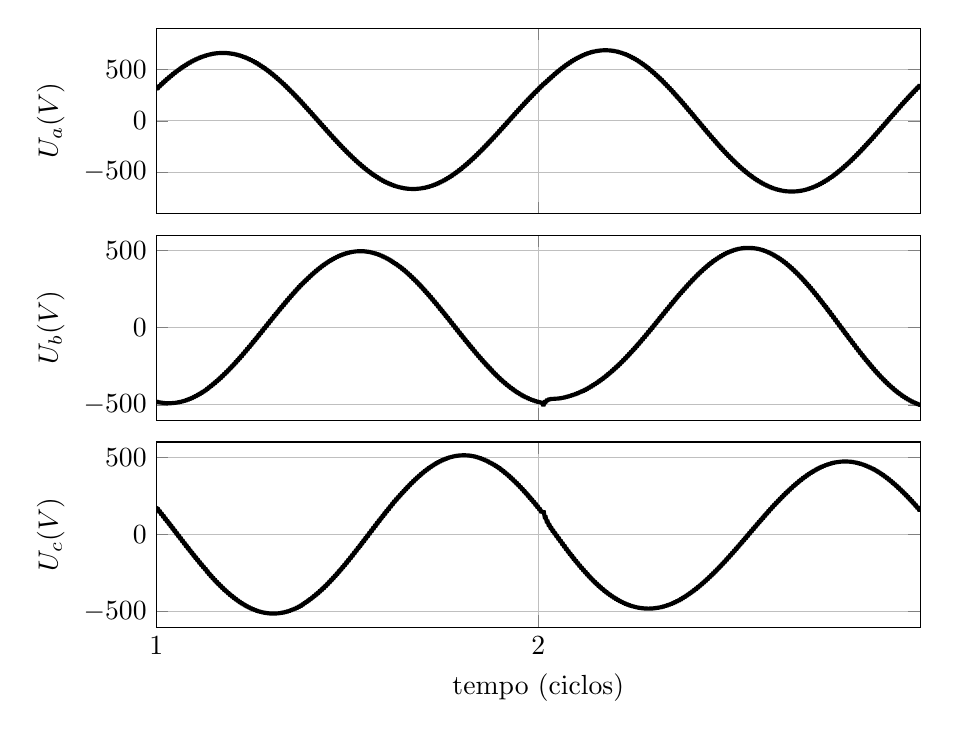
\begin{tikzpicture}

\begin{axis}[%
width=0.8\textwidth,
height=0.193917089240149\textwidth,
scale only axis,
xmin=0.0166666666666667,
xmax=0.05,
xtick={0,0.0166666666666667,0.0333333333333333},
xticklabels={\empty},
xmajorgrids,
ymin=-600,
ymax=600,
ytick={-500,    0,  500},
ylabel={$\text{U}_\text{b}\text{ (V)}$},
ymajorgrids,
name=plot2,
scaled x ticks = false,
legend columns=-1,
legend style={/tikz/every even column/.append style={column sep=0.3cm}},
legend style={font=\footnotesize}
]
\addplot [color=black,solid,line width=1.5pt,forget plot]
  table[row sep=crcr]{0.0166583333333333	-478.328989103039\\
0.0167	-481.372762295986\\
0.0167416666666667	-481.372762295986\\
0.0167833333333333	-483.944387417357\\
0.016825	-483.944387417357\\
0.0168666666666667	-486.043904769891\\
0.0169083333333333	-486.043904769891\\
0.01695	-487.669342075457\\
0.0169916666666667	-487.669342075457\\
0.0170333333333333	-488.81912329053\\
0.017075	-488.81912329053\\
0.0171166666666667	-489.492376222951\\
0.0171583333333333	-489.492376222951\\
0.0172	-489.689089295181\\
0.0172416666666667	-489.689089295181\\
0.0172833333333333	-489.410057478733\\
0.017325	-489.410057478733\\
0.0173666666666667	-488.656714544629\\
0.0174083333333333	-488.656714544629\\
0.01745	-487.430933830334\\
0.0174916666666667	-487.430933830334\\
0.0175333333333333	-485.734862735459\\
0.017575	-485.734862735459\\
0.0176166666666667	-483.570824107468\\
0.0176583333333333	-483.570824107468\\
0.0177	-480.941176730971\\
0.0177416666666667	-480.941176730971\\
0.0177833333333333	-477.848873406491\\
0.017825	-477.848873406491\\
0.0178666666666667	-474.296687037085\\
0.0179083333333333	-474.296687037085\\
0.01795	-470.287554266504\\
0.0179916666666667	-470.287554266504\\
0.0180333333333333	-465.824994538518\\
0.018075	-465.824994538518\\
0.0181166666666667	-460.912896166831\\
0.0181583333333333	-460.912896166831\\
0.0182	-455.555544349316\\
0.0182416666666667	-455.555544349316\\
0.0182833333333333	-449.757632700212\\
0.018325	-449.757632700212\\
0.0183666666666667	-443.524266807923\\
0.0184083333333333	-443.524266807923\\
0.01845	-436.860963041735\\
0.0184916666666667	-436.860963041735\\
0.0185333333333333	-429.773645406549\\
0.018575	-429.773645406549\\
0.0186166666666667	-422.2686421737\\
0.0186583333333333	-422.2686421737\\
0.0187	-414.352682994809\\
0.0187416666666667	-414.352682994809\\
0.0187833333333333	-406.710604021129\\
0.018825	-406.710604021129\\
0.0188666666666667	-396.968651829484\\
0.0189083333333333	-396.968651829484\\
0.01895	-387.24430030011\\
0.0189916666666667	-387.24430030011\\
0.0190333333333333	-377.413842111121\\
0.019075	-377.413842111121\\
0.0191166666666667	-367.3960735467\\
0.0191583333333333	-367.3960735467\\
0.0192	-357.12553953726\\
0.0192416666666667	-357.12553953726\\
0.0192833333333333	-346.559303382721\\
0.019325	-346.559303382721\\
0.0193666666666667	-335.674936708767\\
0.0194083333333333	-335.674936708767\\
0.01945	-324.465686057335\\
0.0194916666666667	-324.465686057335\\
0.0195333333333333	-312.935239244225\\
0.019575	-312.935239244225\\
0.0196166666666667	-301.093266862382\\
0.0196583333333333	-301.093266862382\\
0.0197	-288.95219973374\\
0.0197416666666667	-288.95219973374\\
0.0197833333333333	-276.525463982029\\
0.019825	-276.525463982029\\
0.0198666666666667	-263.82538033546\\
0.0199083333333333	-263.82538033546\\
0.01995	-250.865057706918\\
0.0199916666666667	-250.865057706918\\
0.0200333333333333	-237.656697428642\\
0.020075	-237.656697428642\\
0.0201166666666667	-224.212271375033\\
0.0201583333333333	-224.212271375033\\
0.0202	-210.543848998092\\
0.0202416666666667	-210.543848998092\\
0.0202833333333333	-196.6637735981\\
0.020325	-196.6637735981\\
0.0203666666666667	-182.584756063204\\
0.0204083333333333	-182.584756063204\\
0.02045	-168.319897946886\\
0.0204916666666667	-168.319897946886\\
0.0205333333333333	-153.882668002172\\
0.020575	-153.882668002172\\
0.0206166666666667	-139.286855686717\\
0.0206583333333333	-139.286855686717\\
0.0207	-124.546519243168\\
0.0207416666666667	-124.546519243168\\
0.0207833333333333	-109.675923407492\\
0.020825	-109.675923407492\\
0.0208666666666667	-94.6884951690301\\
0.0209083333333333	-94.6884951690301\\
0.02095	-79.6023211852309\\
0.0209916666666667	-79.6023211852309\\
0.0210333333333333	-64.4296541414652\\
0.021075	-64.4296541414652\\
0.0211166666666667	-49.1854677870168\\
0.0211583333333333	-49.1854677870168\\
0.0212	-33.8847697005379\\
0.0212416666666667	-33.8847697005379\\
0.0212833333333333	-18.5423320716325\\
0.021325	-18.5423320716325\\
0.0213666666666667	-3.1725945533516\\
0.0214083333333333	-3.1725945533516\\
0.02145	12.2102617721841\\
0.0214916666666667	12.2102617721841\\
0.0215333333333333	27.5921432856442\\
0.021575	27.5921432856442\\
0.0216166666666667	42.9588704890498\\
0.0216583333333333	42.9588704890498\\
0.0217	58.2960537853681\\
0.0217416666666667	58.2960537853681\\
0.0217833333333333	73.5890384864759\\
0.021825	73.5890384864759\\
0.0218666666666667	88.82269659409\\
0.0219083333333333	88.82269659409\\
0.02195	103.982669291038\\
0.0219916666666667	103.982669291038\\
0.0220333333333333	119.053037141893\\
0.022075	119.053037141893\\
0.0221166666666667	134.01853586672\\
0.0221583333333333	134.01853586672\\
0.0222	148.863909368128\\
0.0222416666666667	148.863909368128\\
0.0222833333333333	163.573956427556\\
0.022325	163.573956427556\\
0.0223666666666667	178.133568427636\\
0.0224083333333333	178.133568427636\\
0.02245	192.527757716713\\
0.0224916666666667	192.527757716713\\
0.0225333333333333	206.741679404245\\
0.022575	206.741679404245\\
0.0226166666666667	220.760649670751\\
0.0226583333333333	220.760649670751\\
0.0227	234.570162946369\\
0.0227416666666667	234.570162946369\\
0.0227833333333333	248.155909263895\\
0.022825	248.155909263895\\
0.0228666666666667	261.687830320942\\
0.0229083333333333	261.687830320942\\
0.02295	274.986604079196\\
0.0229916666666667	274.986604079196\\
0.0230333333333333	286.928801747272\\
0.023075	286.928801747272\\
0.0231166666666667	298.950506950644\\
0.0231583333333333	298.950506950644\\
0.0232	310.924864102034\\
0.0232416666666667	310.924864102034\\
0.0232833333333333	322.756989832147\\
0.023325	322.756989832147\\
0.0233666666666667	334.367084014297\\
0.0234083333333333	334.367084014297\\
0.02345	345.69602196514\\
0.0234916666666667	345.69602196514\\
0.0235333333333333	356.703461032175\\
0.023575	356.703461032175\\
0.0236166666666667	367.363371170442\\
0.0236583333333333	367.363371170442\\
0.0237	377.659204280424\\
0.0237416666666667	377.659204280424\\
0.0237833333333333	387.579795487262\\
0.023825	387.579795487262\\
0.0238666666666667	397.116425283701\\
0.0239083333333333	397.116425283701\\
0.02395	406.261310362139\\
0.0239916666666667	406.261310362139\\
0.0240333333333333	415.0053223807\\
0.024075	415.0053223807\\
0.0241166666666667	423.340732147141\\
0.0241583333333333	423.340732147141\\
0.0242	431.258683016742\\
0.0242416666666667	431.258683016742\\
0.0242833333333333	438.750365395371\\
0.024325	438.750365395371\\
0.0243666666666667	445.807262831054\\
0.0244083333333333	445.807262831054\\
0.02445	452.421342397773\\
0.0244916666666667	452.421342397773\\
0.0245333333333333	458.585161293933\\
0.024575	458.585161293933\\
0.0246166666666667	464.291905294308\\
0.0246583333333333	464.291905294308\\
0.0247	469.535383109734\\
0.0247416666666667	469.535383109734\\
0.0247833333333333	474.309999446141\\
0.024825	474.309999446141\\
0.0248666666666667	478.610723480444\\
0.0249083333333333	478.610723480444\\
0.02495	482.432523836755\\
0.0249916666666667	482.432523836755\\
0.0250333333333333	485.772612186125\\
0.025075	485.772612186125\\
0.0251166666666667	488.627883686145\\
0.0251583333333333	488.627883686145\\
0.0252	490.994391489966\\
0.0252416666666667	490.994391489966\\
0.0252833333333333	492.869784189106\\
0.025325	492.869784189106\\
0.0253666666666667	494.252063559781\\
0.0254083333333333	494.252063559781\\
0.02545	495.139387583695\\
0.0254916666666667	495.139387583695\\
0.0255333333333333	495.530061759552\\
0.025575	495.530061759552\\
0.0256166666666667	495.422663936061\\
0.0256583333333333	495.422663936061\\
0.0257	494.816230581684\\
0.0257416666666667	494.816230581684\\
0.0257833333333333	493.710425995119\\
0.025825	493.710425995119\\
0.0258666666666667	492.105654148384\\
0.0259083333333333	492.105654148384\\
0.02595	490.003108134894\\
0.0259916666666667	490.003108134894\\
0.0260333333333333	487.404961487327\\
0.026075	487.404961487327\\
0.0261166666666667	484.313069214194\\
0.0261583333333333	484.313069214194\\
0.0262	480.731558886196\\
0.0262416666666667	480.731558886196\\
0.0262833333333333	476.664323712434\\
0.026325	476.664323712434\\
0.0263666666666667	472.115829454631\\
0.0264083333333333	472.115829454631\\
0.02645	467.091068733291\\
0.0264916666666667	467.091068733291\\
0.0265333333333333	461.595540479995\\
0.026575	461.595540479995\\
0.0266166666666667	455.635234907076\\
0.0266583333333333	455.635234907076\\
0.0267	449.21662231492\\
0.0267416666666667	449.21662231492\\
0.0267833333333333	442.346643428456\\
0.026825	442.346643428456\\
0.0268666666666667	435.032699614098\\
0.0269083333333333	435.032699614098\\
0.02695	427.282642172915\\
0.0269916666666667	427.282642172915\\
0.0270333333333333	418.527982244731\\
0.027075	418.527982244731\\
0.0271166666666667	410.672570182659\\
0.0271583333333333	410.672570182659\\
0.0272	402.276872290978\\
0.0272416666666667	402.276872290978\\
0.0272833333333333	393.223850223727\\
0.027325	393.223850223727\\
0.0273666666666667	383.609151155178\\
0.0274083333333333	383.609151155178\\
0.02745	373.508718653929\\
0.0274916666666667	373.508718653929\\
0.0275333333333333	362.979579538073\\
0.027575	362.979579538073\\
0.0276166666666667	352.061894709897\\
0.0276583333333333	352.061894709897\\
0.0277	340.783205444461\\
0.0277416666666667	340.783205444461\\
0.0277833333333333	329.162781541968\\
0.027825	329.162781541968\\
0.0278666666666667	317.215226351439\\
0.0279083333333333	317.215226351439\\
0.02795	304.953068995059\\
0.0279916666666667	304.953068995059\\
0.0280333333333333	292.388308765939\\
0.028075	292.388308765939\\
0.0281166666666667	279.533394256386\\
0.0281583333333333	279.533394256386\\
0.0282	266.401997020689\\
0.0282416666666667	266.401997020689\\
0.0282833333333333	253.007121767018\\
0.028325	253.007121767018\\
0.0283666666666667	239.363037342399\\
0.0284083333333333	239.363037342399\\
0.02845	225.484309796947\\
0.0284916666666667	225.484309796947\\
0.0285333333333333	211.385672071801\\
0.028575	211.385672071801\\
0.0286166666666667	197.081935254737\\
0.0286583333333333	197.081935254737\\
0.0287	182.587950486431\\
0.0287416666666667	182.587950486431\\
0.0287833333333333	167.918604082923\\
0.028825	167.918604082923\\
0.0288666666666667	153.088829011011\\
0.0289083333333333	153.088829011011\\
0.02895	138.113619934855\\
0.0289916666666667	138.113619934855\\
0.0290333333333333	123.008044204917\\
0.029075	123.008044204917\\
0.0291166666666667	107.788100944899\\
0.0291583333333333	107.788100944899\\
0.0292	92.4664220892656\\
0.0292416666666667	92.4664220892656\\
0.0292833333333333	77.0599110293703\\
0.029325	77.0599110293703\\
0.0293666666666667	61.5839402726698\\
0.0294083333333333	61.5839402726698\\
0.02945	46.0538191073489\\
0.0294916666666667	46.0538191073489\\
0.0295333333333333	30.4851141949034\\
0.029575	30.4851141949034\\
0.0296166666666667	14.8937682112207\\
0.0296583333333333	14.8937682112207\\
0.0297	-0.703957306529608\\
0.0297416666666667	-0.703957306529608\\
0.0297833333333333	-16.2916492298269\\
0.029825	-16.2916492298269\\
0.0298666666666667	-31.8529362123827\\
0.0299083333333333	-31.8529362123827\\
0.02995	-47.371649369948\\
0.0299916666666667	-47.371649369948\\
0.0300333333333333	-62.8319222299047\\
0.030075	-62.8319222299047\\
0.0301166666666667	-78.2183969102601\\
0.0301583333333333	-78.2183969102601\\
0.0302	-93.5154108314719\\
0.0302416666666667	-93.5154108314719\\
0.0302833333333333	-108.70816278091\\
0.030325	-108.70816278091\\
0.0303666666666667	-123.782356080195\\
0.0304083333333333	-123.782356080195\\
0.03045	-138.723507249364\\
0.0304916666666667	-138.723507249364\\
0.0305333333333333	-153.517339096442\\
0.030575	-153.517339096442\\
0.0306166666666667	-168.149764544084\\
0.0306583333333333	-168.149764544084\\
0.0307	-182.60688669631\\
0.0307416666666667	-182.60688669631\\
0.0307833333333333	-196.875004412733\\
0.030825	-196.875004412733\\
0.0308666666666667	-210.940621254231\\
0.0309083333333333	-210.940621254231\\
0.03095	-224.790455634942\\
0.0309916666666667	-224.790455634942\\
0.0310333333333333	-238.411450801645\\
0.031075	-238.411450801645\\
0.0311166666666667	-251.788204920739\\
0.0311583333333333	-251.788204920739\\
0.0312	-264.319493294975\\
0.0312416666666667	-264.319493294975\\
0.0312833333333333	-278.081845363642\\
0.031325	-278.081845363642\\
0.0313666666666667	-291.211888263673\\
0.0314083333333333	-291.211888263673\\
0.03145	-303.807007713181\\
0.0314916666666667	-303.807007713181\\
0.0315333333333333	-315.936364357588\\
0.031575	-315.936364357588\\
0.0316166666666667	-327.655020751537\\
0.0316583333333333	-327.655020751537\\
0.0317	-338.998550237152\\
0.0317416666666667	-338.998550237152\\
0.0317833333333333	-349.984949605885\\
0.031825	-349.984949605885\\
0.0318666666666667	-360.618974262017\\
0.0319083333333333	-360.618974262017\\
0.03195	-370.896795074955\\
0.0319916666666667	-370.896795074955\\
0.0320333333333333	-380.809923421548\\
0.032075	-380.809923421548\\
0.0321166666666667	-390.348041070204\\
0.0321583333333333	-390.348041070204\\
0.0322	-399.500455565927\\
0.0322416666666667	-399.500455565927\\
0.0322833333333333	-408.258433783543\\
0.032325	-408.258433783543\\
0.0323666666666667	-416.612673979994\\
0.0324083333333333	-416.612673979994\\
0.03245	-424.555376388038\\
0.0324916666666667	-424.555376388038\\
0.0325333333333333	-432.079651399668\\
0.032575	-432.079651399668\\
0.0326166666666667	-439.17912856472\\
0.0326583333333333	-439.17912856472\\
0.0327	-445.847803165625\\
0.0327416666666667	-445.847803165625\\
0.0327833333333333	-452.079952433882\\
0.032825	-452.079952433882\\
0.0328666666666667	-457.870112681898\\
0.0329083333333333	-457.870112681898\\
0.03295	-463.213095942823\\
0.0329916666666667	-463.213095942823\\
0.0330333333333333	-468.104025539882\\
0.033075	-468.104025539882\\
0.0331166666666667	-472.538375275198\\
0.0331583333333333	-472.538375275198\\
0.0332	-476.512043591712\\
0.0332416666666667	-476.512043591712\\
0.0332833333333333	-480.021998518076\\
0.033325	-480.021998518076\\
0.0333666666666667	-483.062409528906\\
0.0334083333333333	-483.062409528906\\
0.03345	-485.632179354782\\
0.0334916666666667	-485.632179354782\\
0.0335333333333333	-498.998270566993\\
0.033575	-498.998270566993\\
0.0336166666666667	-481.782582963858\\
0.0336583333333333	-481.782582963858\\
0.0337	-471.288948850027\\
0.0337416666666667	-471.288948850027\\
0.0337833333333333	-465.459114040876\\
0.033825	-465.459114040876\\
0.0338666666666667	-462.647848629665\\
0.0339083333333333	-462.647848629665\\
0.03395	-461.417560400509\\
0.0339916666666667	-461.417560400509\\
0.0340333333333333	-460.731633382674\\
0.034075	-460.731633382674\\
0.0341166666666667	-459.951982625119\\
0.0341583333333333	-459.951982625119\\
0.0342	-458.758531093\\
0.0342416666666667	-458.758531093\\
0.0342833333333333	-457.045782912744\\
0.034325	-457.045782912744\\
0.0343666666666667	-454.82926213895\\
0.0344083333333333	-454.82926213895\\
0.03445	-452.172796925181\\
0.0344916666666667	-452.172796925181\\
0.0345333333333333	-449.145658792875\\
0.034575	-449.145658792875\\
0.0346166666666667	-445.800265404507\\
0.0346583333333333	-445.800265404507\\
0.0347	-442.166059354816\\
0.0347416666666667	-442.166059354816\\
0.0347833333333333	-438.252372103144\\
0.034825	-438.252372103144\\
0.0348666666666667	-434.054953798003\\
0.0349083333333333	-434.054953798003\\
0.03495	-429.562674435509\\
0.0349916666666667	-429.562674435509\\
0.0350333333333333	-424.762700040261\\
0.035075	-424.762700040261\\
0.0351166666666667	-419.643661421394\\
0.0351583333333333	-419.643661421394\\
0.0352	-414.197053720857\\
0.0352416666666667	-414.197053720857\\
0.0352833333333333	-408.523882649902\\
0.035325	-408.523882649902\\
0.0353666666666667	-402.479291356868\\
0.0354083333333333	-402.479291356868\\
0.03545	-395.601828599323\\
0.0354916666666667	-395.601828599323\\
0.0355333333333333	-388.546283162184\\
0.035575	-388.546283162184\\
0.0356166666666667	-381.262052118517\\
0.0356583333333333	-381.262052118517\\
0.0357	-373.714229076942\\
0.0357416666666667	-373.714229076942\\
0.0357833333333333	-365.874593646954\\
0.035825	-365.874593646954\\
0.0358666666666667	-357.724034021534\\
0.0359083333333333	-357.724034021534\\
0.03595	-349.251553064004\\
0.0359916666666667	-349.251553064004\\
0.0360333333333333	-340.452622235918\\
0.036075	-340.452622235918\\
0.0361166666666667	-331.327227991727\\
0.0361583333333333	-331.327227991727\\
0.0362	-321.878129980668\\
0.0362416666666667	-321.878129980668\\
0.0362833333333333	-312.109568466451\\
0.036325	-312.109568466451\\
0.0363666666666667	-302.026644843582\\
0.0364083333333333	-302.026644843582\\
0.03645	-291.63387748511\\
0.0364916666666667	-291.63387748511\\
0.0365333333333333	-280.937199605059\\
0.036575	-280.937199605059\\
0.0366166666666667	-269.942114366078\\
0.0366583333333333	-269.942114366078\\
0.0367	-258.654477866822\\
0.0367416666666667	-258.654477866822\\
0.0367833333333333	-247.080567388712\\
0.036825	-247.080567388712\\
0.0368666666666667	-235.227176729096\\
0.0369083333333333	-235.227176729096\\
0.03695	-223.101681785848\\
0.0369916666666667	-223.101681785848\\
0.0370333333333333	-210.712058862678\\
0.037075	-210.712058862678\\
0.0371166666666667	-198.066879573849\\
0.0371583333333333	-198.066879573849\\
0.0372	-185.175292454286\\
0.0372416666666667	-185.175292454286\\
0.0372833333333333	-172.046999319569\\
0.037325	-172.046999319569\\
0.0373666666666667	-158.692016960269\\
0.0374083333333333	-158.692016960269\\
0.03745	-145.121500911102\\
0.0374916666666667	-145.121500911102\\
0.0375333333333333	-131.346961858294\\
0.037575	-131.346961858294\\
0.0376166666666667	-117.380802663719\\
0.0376583333333333	-117.380802663719\\
0.0377	-103.235234173154\\
0.0377416666666667	-103.235234173154\\
0.0377833333333333	-88.9164304808335\\
0.037825	-88.9164304808335\\
0.0378666666666667	-74.439342100256\\
0.0379083333333333	-74.439342100256\\
0.03795	-59.8184609425996\\
0.0379916666666667	-59.8184609425996\\
0.0380333333333333	-45.0680374599692\\
0.038075	-45.0680374599692\\
0.0381166666666667	-30.2022370755135\\
0.0381583333333333	-30.2022370755135\\
0.0382	-15.2353217495658\\
0.0382416666666667	-15.2353217495658\\
0.0382833333333333	-0.181794007753641\\
0.038325	-0.181794007753641\\
0.0383666666666667	14.9435042350192\\
0.0384083333333333	14.9435042350192\\
0.03845	30.1252956286667\\
0.0384916666666667	30.1252956286667\\
0.0385333333333333	45.3486629556394\\
0.038575	45.3486629556394\\
0.0386166666666667	60.5972401707852\\
0.0386583333333333	60.5972401707852\\
0.0387	75.8549297738552\\
0.0387416666666667	75.8549297738552\\
0.0387833333333333	91.1054325668948\\
0.038825	91.1054325668948\\
0.0388666666666667	106.332243601449\\
0.0389083333333333	106.332243601449\\
0.03895	121.518722394686\\
0.0389916666666667	121.518722394686\\
0.0390333333333333	136.648130986171\\
0.039075	136.648130986171\\
0.0391166666666667	151.703658745296\\
0.0391583333333333	151.703658745296\\
0.0392	166.6684438936\\
0.0392416666666667	166.6684438936\\
0.0392833333333333	181.525594900189\\
0.039325	181.525594900189\\
0.0393666666666667	196.258213496354\\
0.0394083333333333	196.258213496354\\
0.03945	211.11916789107\\
0.0394916666666667	211.11916789107\\
0.0395333333333333	225.228256753655\\
0.039575	225.228256753655\\
0.0396166666666667	239.176704133903\\
0.0396583333333333	239.176704133903\\
0.0397	253.050541633453\\
0.0397416666666667	253.050541633453\\
0.0397833333333333	266.794622440343\\
0.039825	266.794622440343\\
0.0398666666666667	280.36352639823\\
0.0399083333333333	280.36352639823\\
0.03995	293.720079804169\\
0.0399916666666667	293.720079804169\\
0.0400333333333333	306.834840978919\\
0.040075	306.834840978919\\
0.0401166666666667	319.684432072053\\
0.0401583333333333	319.684432072053\\
0.0402	332.249529221863\\
0.0402416666666667	332.249529221863\\
0.0402833333333333	344.513518148991\\
0.040325	344.513518148991\\
0.0403666666666667	356.461398472636\\
0.0404083333333333	356.461398472636\\
0.04045	368.07906117244\\
0.0404916666666667	368.07906117244\\
0.0405333333333333	379.352665704272\\
0.040575	379.352665704272\\
0.0406166666666667	390.268254951875\\
0.0406583333333333	390.268254951875\\
0.0407	400.81284512302\\
0.0407416666666667	400.81284512302\\
0.0407833333333333	410.973175722926\\
0.040825	410.973175722926\\
0.0408666666666667	420.736369760103\\
0.0409083333333333	420.736369760103\\
0.04095	430.089939730837\\
0.0409916666666667	430.089939730837\\
0.0410333333333333	439.02189748336\\
0.041075	439.02189748336\\
0.0411166666666667	447.520797951081\\
0.0411583333333333	447.520797951081\\
0.0412	455.57576068455\\
0.0412416666666667	455.57576068455\\
0.0412833333333333	463.176477754051\\
0.041325	463.176477754051\\
0.0413666666666667	470.313215198367\\
0.0414083333333333	470.313215198367\\
0.04145	476.976813020432\\
0.0414916666666667	476.976813020432\\
0.0415333333333333	483.158335808922\\
0.041575	483.158335808922\\
0.0416166666666667	488.850790106914\\
0.0416583333333333	488.850790106914\\
0.0417	494.046217480564\\
0.0417416666666667	494.046217480564\\
0.0417833333333333	498.740107259914\\
0.041825	498.740107259914\\
0.0418666666666667	502.92186011784\\
0.0419083333333333	502.92186011784\\
0.04195	506.583545623777\\
0.0419916666666667	506.583545623777\\
0.0420333333333333	509.721710214485\\
0.042075	509.721710214485\\
0.0421166666666667	512.332784100593\\
0.0421583333333333	512.332784100593\\
0.0422	514.413279158182\\
0.0422416666666667	514.413279158182\\
0.0422833333333333	515.9599757688\\
0.042325	515.9599757688\\
0.0423666666666667	516.970100515159\\
0.0424083333333333	516.970100515159\\
0.04245	517.441480758459\\
0.0424916666666667	517.441480758459\\
0.0425333333333333	517.372752150282\\
0.042575	517.372752150282\\
0.0426166666666667	516.762847399441\\
0.0426583333333333	516.762847399441\\
0.0427	515.611781315798\\
0.0427416666666667	515.611781315798\\
0.0427833333333333	513.92048533442\\
0.042825	513.92048533442\\
0.0428666666666667	511.690288385606\\
0.0429083333333333	511.690288385606\\
0.04295	508.923157960981\\
0.0429916666666667	508.923157960981\\
0.0430333333333333	505.62173995849\\
0.043075	505.62173995849\\
0.0431166666666667	501.78931073118\\
0.0431583333333333	501.78931073118\\
0.0432	497.429767725351\\
0.0432416666666667	497.429767725351\\
0.0432833333333333	492.547621632959\\
0.043325	492.547621632959\\
0.0433666666666667	487.14798908254\\
0.0434083333333333	487.14798908254\\
0.04345	481.236584761708\\
0.0434916666666667	481.236584761708\\
0.0435333333333333	474.813193437904\\
0.043575	474.813193437904\\
0.0436166666666667	467.617975016633\\
0.0436583333333333	467.617975016633\\
0.0437	460.640009785613\\
0.0437416666666667	460.640009785613\\
0.0437833333333333	453.026742559859\\
0.043825	453.026742559859\\
0.0438666666666667	444.829079350061\\
0.0439083333333333	444.829079350061\\
0.04395	436.091902638318\\
0.0439916666666667	436.091902638318\\
0.0440333333333333	426.854279959608\\
0.044075	426.854279959608\\
0.0441166666666667	417.147056125927\\
0.0441583333333333	417.147056125927\\
0.0442	406.993617805562\\
0.0442416666666667	406.993617805562\\
0.0442833333333333	396.411764190075\\
0.044325	396.411764190075\\
0.0443666666666667	385.415729474773\\
0.0444083333333333	385.415729474773\\
0.04445	374.017909476246\\
0.0444916666666667	374.017909476246\\
0.0445333333333333	362.230108715941\\
0.044575	362.230108715941\\
0.0446166666666667	350.064119512135\\
0.0446583333333333	350.064119512135\\
0.0447	337.533091230516\\
0.0447416666666667	337.533091230516\\
0.0447833333333333	324.649922144971\\
0.044825	324.649922144971\\
0.0448666666666667	311.428439890778\\
0.0449083333333333	311.428439890778\\
0.04495	297.883125554185\\
0.0449916666666667	297.883125554185\\
0.0450333333333333	284.028841924275\\
0.045075	284.028841924275\\
0.0451166666666667	269.880782608134\\
0.0451583333333333	269.880782608134\\
0.0452	255.454385329104\\
0.0452416666666667	255.454385329104\\
0.0452833333333333	240.765301798375\\
0.045325	240.765301798375\\
0.0453666666666667	225.829384538562\\
0.0454083333333333	225.829384538562\\
0.04545	210.662681339409\\
0.0454916666666667	210.662681339409\\
0.0455333333333333	195.281430438134\\
0.045575	195.281430438134\\
0.0456166666666667	179.702077212704\\
0.0456583333333333	179.702077212704\\
0.0457	163.941485539902\\
0.0457416666666667	163.941485539902\\
0.0457833333333333	148.015394086019\\
0.045825	148.015394086019\\
0.0458666666666667	131.941232581943\\
0.0459083333333333	131.941232581943\\
0.04595	115.733018226992\\
0.0459916666666667	115.733018226992\\
0.0460333333333333	99.4155506737076\\
0.046075	99.4155506737076\\
0.0461166666666667	83.0048753817104\\
0.0461583333333333	83.0048753817104\\
0.0462	66.5169842374124\\
0.0462416666666667	66.5169842374124\\
0.0462833333333333	49.9685533749797\\
0.046325	49.9685533749797\\
0.0463666666666667	33.3767580588298\\
0.0464083333333333	33.3767580588298\\
0.04645	16.7590504552267\\
0.0464916666666667	16.7590504552267\\
0.0465333333333333	0.132970181758703\\
0.046575	0.132970181758703\\
0.0466166666666667	-16.4839901619608\\
0.0466583333333333	-16.4839901619608\\
0.0467	-33.0746636693815\\
0.0467416666666667	-33.0746636693815\\
0.0467833333333333	-49.6211722773108\\
0.046825	-49.6211722773108\\
0.0468666666666667	-66.1070457181566\\
0.0469083333333333	-66.1070457181566\\
0.04695	-82.5154452365718\\
0.0469916666666667	-82.5154452365718\\
0.0470333333333333	-98.8296440709486\\
0.047075	-98.8296440709486\\
0.0471166666666667	-115.033091242092\\
0.0471583333333333	-115.033091242092\\
0.0472	-131.109433370824\\
0.0472416666666667	-131.109433370824\\
0.0472833333333333	-147.042503492819\\
0.047325	-147.042503492819\\
0.0473666666666667	-162.816333505291\\
0.0474083333333333	-162.816333505291\\
0.04745	-178.41516835848\\
0.0474916666666667	-178.41516835848\\
0.0475333333333333	-193.8234809494\\
0.047575	-193.8234809494\\
0.0476166666666667	-209.025986747927\\
0.0476583333333333	-209.025986747927\\
0.0477	-223.904186047126\\
0.0477416666666667	-223.904186047126\\
0.0477833333333333	-238.606857549563\\
0.047825	-238.606857549563\\
0.0478666666666667	-253.47478702492\\
0.0479083333333333	-253.47478702492\\
0.04795	-267.938417779568\\
0.0479916666666667	-267.938417779568\\
0.0480333333333333	-282.029617204579\\
0.048075	-282.029617204579\\
0.0481166666666667	-295.766635150869\\
0.0481583333333333	-295.766635150869\\
0.0482	-309.161799602257\\
0.0482416666666667	-309.161799602257\\
0.0482833333333333	-322.219833483858\\
0.048325	-322.219833483858\\
0.0483666666666667	-334.938825256652\\
0.0484083333333333	-334.938825256652\\
0.04845	-347.312016422018\\
0.0484916666666667	-347.312016422018\\
0.0485333333333333	-359.329644222863\\
0.048575	-359.329644222863\\
0.0486166666666667	-370.980465786804\\
0.0486583333333333	-370.980465786804\\
0.0487	-382.252844743103\\
0.0487416666666667	-382.252844743103\\
0.0487833333333333	-393.135216849012\\
0.048825	-393.135216849012\\
0.0488666666666667	-403.617584174739\\
0.0489083333333333	-403.617584174739\\
0.04895	-413.689218945276\\
0.0489916666666667	-413.689218945276\\
0.0490333333333333	-423.340771462502\\
0.049075	-423.340771462502\\
0.0491166666666667	-432.563452770036\\
0.0491583333333333	-432.563452770036\\
0.0492	-441.348991482752\\
0.0492416666666667	-441.348991482752\\
0.0492833333333333	-449.689568336581\\
0.049325	-449.689568336581\\
0.0493666666666667	-457.577772446396\\
0.0494083333333333	-457.577772446396\\
0.04945	-465.006594338065\\
0.0494916666666667	-465.006594338065\\
0.0495333333333333	-471.969434299032\\
0.049575	-471.969434299032\\
0.0496166666666667	-478.460118028508\\
0.0496583333333333	-478.460118028508\\
0.0497	-484.472913508959\\
0.0497416666666667	-484.472913508959\\
0.0497833333333333	-490.002697136551\\
0.049825	-490.002697136551\\
0.0498666666666667	-495.044403692677\\
0.0499083333333333	-495.044403692677\\
0.04995	-499.593400120443\\
0.0499916666666667	-499.593400120443\\
};
\end{axis}

\begin{axis}[%
width=0.8\textwidth,
height=0.193917089240149\textwidth,
scale only axis,
xmin=0.0166666666666667,
xmax=0.05,
xtick={0,0.0166666666666667,0.0333333333333333},
xticklabels={{0},{1},{2}},
xlabel={tempo (ciclos)},
xmajorgrids,
ymin=-600,
ymax=600,
ytick={-500,    0,  500},
ylabel={$\text{U}_\text{c}\text{ (V)}$},
ymajorgrids,
at=(plot2.below south west),
anchor=above north west,
scaled x ticks = false,
legend columns=-1,
legend style={/tikz/every even column/.append style={column sep=0.3cm}},
legend style={font=\footnotesize}
]
\addplot [color=black,solid,line width=1.5pt,forget plot]
  table[row sep=crcr]{0.0166583333333333	180.146044285981\\
0.0167	164.940320934484\\
0.0167416666666667	164.940320934484\\
0.0167833333333333	149.579587477261\\
0.016825	149.579587477261\\
0.0168666666666667	134.079551509137\\
0.0169083333333333	134.079551509137\\
0.01695	118.455249604828\\
0.0169916666666667	118.455249604828\\
0.0170333333333333	102.721820759597\\
0.017075	102.721820759597\\
0.0171166666666667	86.8947024886041\\
0.0171583333333333	86.8947024886041\\
0.0172	70.9897152347551\\
0.0172416666666667	70.9897152347551\\
0.0172833333333333	55.0229884605968\\
0.017325	55.0229884605968\\
0.0173666666666667	39.0107951391398\\
0.0174083333333333	39.0107951391398\\
0.01745	22.9693692316446\\
0.0174916666666667	22.9693692316446\\
0.0175333333333333	6.91476165823279\\
0.017575	6.91476165823279\\
0.0176166666666667	-9.13724020053355\\
0.0176583333333333	-9.13724020053355\\
0.0177	-25.1712876244939\\
0.0177416666666667	-25.1712876244939\\
0.0177833333333333	-41.1717016099994\\
0.017825	-41.1717016099994\\
0.0178666666666667	-57.1235450619316\\
0.0179083333333333	-57.1235450619316\\
0.01795	-73.0122416753861\\
0.0179916666666667	-73.0122416753861\\
0.0180333333333333	-88.8229904086394\\
0.018075	-88.8229904086394\\
0.0181166666666667	-104.541092542183\\
0.0181583333333333	-104.541092542183\\
0.0182	-120.151937938219\\
0.0182416666666667	-120.151937938219\\
0.0182833333333333	-135.641005542097\\
0.018325	-135.641005542097\\
0.0183666666666667	-150.993870043721\\
0.0184083333333333	-150.993870043721\\
0.01845	-166.196212093992\\
0.0184916666666667	-166.196212093992\\
0.0185333333333333	-181.2338298443\\
0.018575	-181.2338298443\\
0.0186166666666667	-196.092650491087\\
0.0186583333333333	-196.092650491087\\
0.0187	-210.758741337919\\
0.0187416666666667	-210.758741337919\\
0.0187833333333333	-224.272823986116\\
0.018825	-224.272823986116\\
0.0188666666666667	-239.924185188171\\
0.0189083333333333	-239.924185188171\\
0.01895	-254.795099361687\\
0.0189916666666667	-254.795099361687\\
0.0190333333333333	-269.036557729883\\
0.019075	-269.036557729883\\
0.0191166666666667	-282.760389233867\\
0.0191583333333333	-282.760389233867\\
0.0192	-296.057851197266\\
0.0192416666666667	-296.057851197266\\
0.0192833333333333	-308.990098283122\\
0.019325	-308.990098283122\\
0.0193666666666667	-321.590393418407\\
0.0194083333333333	-321.590393418407\\
0.01945	-333.870571911174\\
0.0194916666666667	-333.870571911174\\
0.0195333333333333	-345.828322444006\\
0.019575	-345.828322444006\\
0.0196166666666667	-357.453508661192\\
0.0196583333333333	-357.453508661192\\
0.0197	-368.732790011102\\
0.0197416666666667	-368.732790011102\\
0.0197833333333333	-379.652185798579\\
0.019825	-379.652185798579\\
0.0198666666666667	-390.200039679523\\
0.0199083333333333	-390.200039679523\\
0.01995	-400.364455853375\\
0.0199916666666667	-400.364455853375\\
0.0200333333333333	-410.135593074462\\
0.020075	-410.135593074462\\
0.0201166666666667	-419.504723697965\\
0.0201583333333333	-419.504723697965\\
0.0202	-428.463752199279\\
0.0202416666666667	-428.463752199279\\
0.0202833333333333	-437.004944992871\\
0.020325	-437.004944992871\\
0.0203666666666667	-445.120779808899\\
0.0204083333333333	-445.120779808899\\
0.02045	-452.8038978512\\
0.0204916666666667	-452.8038978512\\
0.0205333333333333	-460.047124180064\\
0.020575	-460.047124180064\\
0.0206166666666667	-466.843522119401\\
0.0206583333333333	-466.843522119401\\
0.0207	-473.186455823302\\
0.0207416666666667	-473.186455823302\\
0.0207833333333333	-479.069643185327\\
0.020825	-479.069643185327\\
0.0208666666666667	-484.487584080736\\
0.0209083333333333	-484.487584080736\\
0.02095	-489.433644253288\\
0.0209916666666667	-489.433644253288\\
0.0210333333333333	-493.903539136153\\
0.021075	-493.903539136153\\
0.0211166666666667	-497.892633124744\\
0.0211583333333333	-497.892633124744\\
0.0212	-501.396820907034\\
0.0212416666666667	-501.396820907034\\
0.0212833333333333	-504.41270742765\\
0.021325	-504.41270742765\\
0.0213666666666667	-506.937652408911\\
0.0214083333333333	-506.937652408911\\
0.02145	-508.969679717527\\
0.0214916666666667	-508.969679717527\\
0.0215333333333333	-510.507315547184\\
0.021575	-510.507315547184\\
0.0216166666666667	-511.549437470117\\
0.0216583333333333	-511.549437470117\\
0.0217	-512.095173916005\\
0.0217416666666667	-512.095173916005\\
0.0217833333333333	-512.14386626104\\
0.021825	-512.14386626104\\
0.0218666666666667	-511.694775425209\\
0.0219083333333333	-511.694775425209\\
0.02195	-510.748811874119\\
0.0219916666666667	-510.748811874119\\
0.0220333333333333	-509.305240015087\\
0.022075	-509.305240015087\\
0.0221166666666667	-507.364690126307\\
0.0221583333333333	-507.364690126307\\
0.0222	-504.928245184668\\
0.0222416666666667	-504.928245184668\\
0.0222833333333333	-501.997459837756\\
0.022325	-501.997459837756\\
0.0223666666666667	-498.57437873634\\
0.0224083333333333	-498.57437873634\\
0.02245	-494.661546862205\\
0.0224916666666667	-494.661546862205\\
0.0225333333333333	-490.262014038761\\
0.022575	-490.262014038761\\
0.0226166666666667	-485.379336077746\\
0.0226583333333333	-485.379336077746\\
0.0227	-480.017574398345\\
0.0227416666666667	-480.017574398345\\
0.0227833333333333	-474.181295093699\\
0.022825	-474.181295093699\\
0.0228666666666667	-468.132227564933\\
0.0229083333333333	-468.132227564933\\
0.02295	-461.649789032895\\
0.0229916666666667	-461.649789032895\\
0.0230333333333333	-453.193902270209\\
0.023075	-453.193902270209\\
0.0231166666666667	-444.773441113673\\
0.0231583333333333	-444.773441113673\\
0.0232	-436.251268459993\\
0.0232416666666667	-436.251268459993\\
0.0232833333333333	-427.520263672964\\
0.023325	-427.520263672964\\
0.0233666666666667	-418.493740302993\\
0.0234083333333333	-418.493740302993\\
0.02345	-409.11363513705\\
0.0234916666666667	-409.11363513705\\
0.0235333333333333	-399.348350327473\\
0.023575	-399.348350327473\\
0.0236166666666667	-389.186670490501\\
0.0236583333333333	-389.186670490501\\
0.0237	-378.630905372963\\
0.0237416666666667	-378.630905372963\\
0.0237833333333333	-367.690968950489\\
0.023825	-367.690968950489\\
0.0238666666666667	-356.380102358096\\
0.0239083333333333	-356.380102358096\\
0.02395	-344.712640572405\\
0.0239916666666667	-344.712640572405\\
0.0240333333333333	-332.700781505562\\
0.024075	-332.700781505562\\
0.0241166666666667	-320.358317577706\\
0.0241583333333333	-320.358317577706\\
0.0242	-307.6971824162\\
0.0242416666666667	-307.6971824162\\
0.0242833333333333	-294.729044137296\\
0.024325	-294.729044137296\\
0.0243666666666667	-281.465654636295\\
0.0244083333333333	-281.465654636295\\
0.02445	-267.919108296558\\
0.0244916666666667	-267.919108296558\\
0.0245333333333333	-254.101977634579\\
0.024575	-254.101977634579\\
0.0246166666666667	-240.027348361342\\
0.0246583333333333	-240.027348361342\\
0.0247	-225.708789227798\\
0.0247416666666667	-225.708789227798\\
0.0247833333333333	-211.160290317149\\
0.024825	-211.160290317149\\
0.0248666666666667	-196.39619457631\\
0.0249083333333333	-196.39619457631\\
0.02495	-181.431040895376\\
0.0249916666666667	-181.431040895376\\
0.0250333333333333	-166.279778355741\\
0.025075	-166.279778355741\\
0.0251166666666667	-150.957981557132\\
0.0251583333333333	-150.957981557132\\
0.0252	-135.480589084291\\
0.0252416666666667	-135.480589084291\\
0.0252833333333333	-119.863094908503\\
0.025325	-119.863094908503\\
0.0253666666666667	-104.121014925928\\
0.0254083333333333	-104.121014925928\\
0.02545	-88.2697324252375\\
0.0254916666666667	-88.2697324252375\\
0.0255333333333333	-72.3244975934466\\
0.025575	-72.3244975934466\\
0.0256166666666667	-56.3005347394663\\
0.0256583333333333	-56.3005347394663\\
0.0257	-40.2131789209932\\
0.0257416666666667	-40.2131789209932\\
0.0257833333333333	-24.0779930748701\\
0.025825	-24.0779930748701\\
0.0258666666666667	-7.91083206935371\\
0.0259083333333333	-7.91083206935371\\
0.02595	8.27214526930201\\
0.0259916666666667	8.27214526930201\\
0.0260333333333333	24.4542254440382\\
0.026075	24.4542254440382\\
0.0261166666666667	40.6199908695603\\
0.0261583333333333	40.6199908695603\\
0.0262	56.7516612117422\\
0.0262416666666667	56.7516612117422\\
0.0262833333333333	72.8325712785133\\
0.026325	72.8325712785133\\
0.0263666666666667	88.846063325594\\
0.0264083333333333	88.846063325594\\
0.02645	104.775539088676\\
0.0264916666666667	104.775539088676\\
0.0265333333333333	120.604489043941\\
0.026575	120.604489043941\\
0.0266166666666667	136.316517603678\\
0.0266583333333333	136.316517603678\\
0.0267	151.895365005857\\
0.0267416666666667	151.895365005857\\
0.0267833333333333	167.32492740609\\
0.026825	167.32492740609\\
0.0268666666666667	182.589276240632\\
0.0269083333333333	182.589276240632\\
0.02695	197.67267733356\\
0.0269916666666667	197.67267733356\\
0.0270333333333333	213.364075445209\\
0.027075	213.364075445209\\
0.0271166666666667	227.019890089968\\
0.0271583333333333	227.019890089968\\
0.0272	240.616905132375\\
0.0272416666666667	240.616905132375\\
0.0272833333333333	254.329291302055\\
0.027325	254.329291302055\\
0.0273666666666667	268.025476997475\\
0.0274083333333333	268.025476997475\\
0.02745	281.599414976171\\
0.0274916666666667	281.599414976171\\
0.0275333333333333	294.97178527555\\
0.027575	294.97178527555\\
0.0276166666666667	308.087625765951\\
0.0276583333333333	308.087625765951\\
0.0277	320.910690989392\\
0.0277416666666667	320.910690989392\\
0.0277833333333333	333.417415766459\\
0.027825	333.417415766459\\
0.0278666666666667	345.591780478394\\
0.0279083333333333	345.591780478394\\
0.02795	357.421558389868\\
0.0279916666666667	357.421558389868\\
0.0280333333333333	368.896047770843\\
0.028075	368.896047770843\\
0.0281166666666667	380.004638133566\\
0.0281583333333333	380.004638133566\\
0.0282	390.735700889524\\
0.0282416666666667	390.735700889524\\
0.0282833333333333	401.079183264076\\
0.028325	401.079183264076\\
0.0283666666666667	411.023979838759\\
0.0284083333333333	411.023979838759\\
0.02845	420.559255161147\\
0.0284916666666667	420.559255161147\\
0.0285333333333333	429.674638195389\\
0.028575	429.674638195389\\
0.0286166666666667	438.36034696872\\
0.0286583333333333	438.36034696872\\
0.0287	446.607237052018\\
0.0287416666666667	446.607237052018\\
0.0287833333333333	454.406798841608\\
0.028825	454.406798841608\\
0.0288666666666667	461.751128592088\\
0.0289083333333333	461.751128592088\\
0.02895	468.632892411405\\
0.0289916666666667	468.632892411405\\
0.0290333333333333	475.045294902946\\
0.029075	475.045294902946\\
0.0291166666666667	480.981879753185\\
0.0291583333333333	480.981879753185\\
0.0292	486.437323221531\\
0.0292416666666667	486.437323221531\\
0.0292833333333333	491.406267662622\\
0.029325	491.406267662622\\
0.0293666666666667	495.883928335018\\
0.0294083333333333	495.883928335018\\
0.02945	499.866055615843\\
0.0294916666666667	499.866055615843\\
0.0295333333333333	503.348727665725\\
0.029575	503.348727665725\\
0.0296166666666667	506.32826432485\\
0.0296583333333333	506.32826432485\\
0.0297	508.801283597195\\
0.0297416666666667	508.801283597195\\
0.0297833333333333	510.764841924053\\
0.029825	510.764841924053\\
0.0298666666666667	512.216584774959\\
0.0299083333333333	512.216584774959\\
0.02995	513.154859732115\\
0.0299916666666667	513.154859732115\\
0.0300333333333333	513.578772270348\\
0.030075	513.578772270348\\
0.0301166666666667	513.488424330974\\
0.0301583333333333	513.488424330974\\
0.0302	512.883757056606\\
0.0302416666666667	512.883757056606\\
0.0302833333333333	511.766137250959\\
0.030325	511.766137250959\\
0.0303666666666667	510.137917947873\\
0.0304083333333333	510.137917947873\\
0.03045	508.001445961413\\
0.0304916666666667	508.001445961413\\
0.0305333333333333	505.359600176138\\
0.030575	505.359600176138\\
0.0306166666666667	502.215762753867\\
0.0306583333333333	502.215762753867\\
0.0307	498.573803881371\\
0.0307416666666667	498.573803881371\\
0.0307833333333333	494.438070082401\\
0.030825	494.438070082401\\
0.0308666666666667	489.813374792093\\
0.0309083333333333	489.813374792093\\
0.03095	484.704989725497\\
0.0309916666666667	484.704989725497\\
0.0310333333333333	479.118636144247\\
0.031075	479.118636144247\\
0.0311166666666667	473.056878981776\\
0.0311583333333333	473.056878981776\\
0.0312	465.70497451635\\
0.0312416666666667	465.70497451635\\
0.0312833333333333	459.969396284381\\
0.031325	459.969396284381\\
0.0313666666666667	453.306592780928\\
0.0314083333333333	453.306592780928\\
0.03145	445.858568368547\\
0.0314916666666667	445.858568368547\\
0.0315333333333333	437.745808877649\\
0.031575	437.745808877649\\
0.0316166666666667	429.069979853876\\
0.0316583333333333	429.069979853876\\
0.0317	419.905934001149\\
0.0317416666666667	419.905934001149\\
0.0317833333333333	410.303765791928\\
0.031825	410.303765791928\\
0.0318666666666667	400.294607272454\\
0.0319083333333333	400.294607272454\\
0.03195	389.897105361559\\
0.0319916666666667	389.897105361559\\
0.0320333333333333	379.123044209476\\
0.032075	379.123044209476\\
0.0321166666666667	367.981436719615\\
0.0321583333333333	367.981436719615\\
0.0322	356.480648193397\\
0.0322416666666667	356.480648193397\\
0.0322833333333333	344.631665623135\\
0.032325	344.631665623135\\
0.0323666666666667	332.444618169672\\
0.0324083333333333	332.444618169672\\
0.03245	319.931569517662\\
0.0324916666666667	319.931569517662\\
0.0325333333333333	307.105674240986\\
0.032575	307.105674240986\\
0.0326166666666667	293.98058862761\\
0.0326583333333333	293.98058862761\\
0.0327	280.570215241566\\
0.0327416666666667	280.570215241566\\
0.0327833333333333	266.888552880234\\
0.032825	266.888552880234\\
0.0328666666666667	252.949637821179\\
0.0329083333333333	252.949637821179\\
0.03295	238.76754490619\\
0.0329916666666667	238.76754490619\\
0.0330333333333333	224.356417917444\\
0.033075	224.356417917444\\
0.0331166666666667	209.730506383327\\
0.0331583333333333	209.730506383327\\
0.0332	194.904179567313\\
0.0332416666666667	194.904179567313\\
0.0332833333333333	179.892215293915\\
0.033325	179.892215293915\\
0.0333666666666667	164.708751896154\\
0.0334083333333333	164.708751896154\\
0.03345	149.368805147729\\
0.0334916666666667	149.368805147729\\
0.0335333333333333	144.726395351648\\
0.033575	144.726395351648\\
0.0336166666666667	111.518693770504\\
0.0336583333333333	111.518693770504\\
0.0337	84.4850628016701\\
0.0337416666666667	84.4850628016701\\
0.0337833333333333	61.8484278857143\\
0.033825	61.8484278857143\\
0.0338666666666667	42.2155441006047\\
0.0339083333333333	42.2155441006047\\
0.03395	24.3436843215581\\
0.0339916666666667	24.3436843215581\\
0.0340333333333333	7.33008530013169\\
0.034075	7.33008530013169\\
0.0341166666666667	-9.38060315559805\\
0.0341583333333333	-9.38060315559805\\
0.0342	-26.0621031757783\\
0.0342416666666667	-26.0621031757783\\
0.0342833333333333	-42.7956768143287\\
0.034325	-42.7956768143287\\
0.0343666666666667	-59.552038808165\\
0.0344083333333333	-59.552038808165\\
0.03445	-76.2573097499925\\
0.0344916666666667	-76.2573097499925\\
0.0345333333333333	-92.8312571699922\\
0.034575	-92.8312571699922\\
0.0346166666666667	-109.208264129288\\
0.0346583333333333	-109.208264129288\\
0.0347	-125.343508819151\\
0.0347416666666667	-125.343508819151\\
0.0347833333333333	-141.210871672277\\
0.034825	-141.210871672277\\
0.0348666666666667	-156.797339101969\\
0.0349083333333333	-156.797339101969\\
0.03495	-172.09708609055\\
0.0349916666666667	-172.09708609055\\
0.0350333333333333	-187.10682129861\\
0.035075	-187.10682129861\\
0.0351166666666667	-201.822884021664\\
0.0351583333333333	-201.822884021664\\
0.0352	-216.239919470703\\
0.0352416666666667	-216.239919470703\\
0.0352833333333333	-230.202213824371\\
0.035325	-230.202213824371\\
0.0353666666666667	-243.896227334877\\
0.0354083333333333	-243.896227334877\\
0.03545	-257.954073023585\\
0.0354916666666667	-257.954073023585\\
0.0355333333333333	-271.461318155762\\
0.035575	-271.461318155762\\
0.0356166666666667	-284.47339582563\\
0.0356583333333333	-284.47339582563\\
0.0357	-297.031539241408\\
0.0357416666666667	-297.031539241408\\
0.0357833333333333	-309.168581031362\\
0.035825	-309.168581031362\\
0.0358666666666667	-320.905622029561\\
0.0359083333333333	-320.905622029561\\
0.03595	-332.253232016136\\
0.0359916666666667	-332.253232016136\\
0.0360333333333333	-343.213835424223\\
0.036075	-343.213835424223\\
0.0361166666666667	-353.784534698212\\
0.0361583333333333	-353.784534698212\\
0.0362	-363.959618715826\\
0.0362416666666667	-363.959618715826\\
0.0362833333333333	-373.732416364792\\
0.036325	-373.732416364792\\
0.0363666666666667	-383.09618677639\\
0.0364083333333333	-383.09618677639\\
0.03645	-392.046125811641\\
0.0364916666666667	-392.046125811641\\
0.0365333333333333	-400.576614093654\\
0.036575	-400.576614093654\\
0.0366166666666667	-408.68372435094\\
0.0366583333333333	-408.68372435094\\
0.0367	-416.364165112605\\
0.0367416666666667	-416.364165112605\\
0.0367833333333333	-423.615145447101\\
0.036825	-423.615145447101\\
0.0368666666666667	-430.434233741803\\
0.0369083333333333	-430.434233741803\\
0.03695	-436.819261059435\\
0.0369916666666667	-436.819261059435\\
0.0370333333333333	-442.768283150409\\
0.037075	-442.768283150409\\
0.0371166666666667	-448.279573831794\\
0.0371583333333333	-448.279573831794\\
0.0372	-453.351635224766\\
0.0372416666666667	-453.351635224766\\
0.0372833333333333	-457.983213481598\\
0.037325	-457.983213481598\\
0.0373666666666667	-462.173298142092\\
0.0374083333333333	-462.173298142092\\
0.03745	-465.921310882512\\
0.0374916666666667	-465.921310882512\\
0.0375333333333333	-469.226475073581\\
0.037575	-469.226475073581\\
0.0376166666666667	-472.087628414329\\
0.0376583333333333	-472.087628414329\\
0.0377	-474.504739536445\\
0.0377416666666667	-474.504739536445\\
0.0377833333333333	-476.484218816971\\
0.037825	-476.484218816971\\
0.0378666666666667	-478.025004478011\\
0.0379083333333333	-478.025004478011\\
0.03795	-479.127000034947\\
0.0379916666666667	-479.127000034947\\
0.0380333333333333	-479.790853044839\\
0.038075	-479.790853044839\\
0.0381166666666667	-480.017810383355\\
0.0381583333333333	-480.017810383355\\
0.0382	-479.809550640255\\
0.0382416666666667	-479.809550640255\\
0.0382833333333333	-479.168048698886\\
0.038325	-479.168048698886\\
0.0383666666666667	-478.09547161042\\
0.0384083333333333	-478.09547161042\\
0.03845	-476.594029513009\\
0.0384916666666667	-476.594029513009\\
0.0385333333333333	-474.667087536517\\
0.038575	-474.667087536517\\
0.0386166666666667	-472.316613748042\\
0.0386583333333333	-472.316613748042\\
0.0387	-469.545524854984\\
0.0387416666666667	-469.545524854984\\
0.0387833333333333	-466.356973227985\\
0.038825	-466.356973227985\\
0.0388666666666667	-462.754319555445\\
0.0389083333333333	-462.754319555445\\
0.03895	-458.741174214815\\
0.0389916666666667	-458.741174214815\\
0.0390333333333333	-454.321410232606\\
0.039075	-454.321410232606\\
0.0391166666666667	-449.499164302465\\
0.0391583333333333	-449.499164302465\\
0.0392	-444.278834824636\\
0.0392416666666667	-444.278834824636\\
0.0392833333333333	-438.665079740591\\
0.039325	-438.665079740591\\
0.0393666666666667	-432.662815692646\\
0.0394083333333333	-432.662815692646\\
0.03945	-426.653469373525\\
0.0394916666666667	-426.653469373525\\
0.0395333333333333	-419.443762928223\\
0.039575	-419.443762928223\\
0.0396166666666667	-411.87604861213\\
0.0396583333333333	-411.87604861213\\
0.0397	-404.105575137083\\
0.0397416666666667	-404.105575137083\\
0.0397833333333333	-396.085701802544\\
0.039825	-396.085701802544\\
0.0398666666666667	-387.781743231563\\
0.0399083333333333	-387.781743231563\\
0.03995	-379.170623976712\\
0.0399916666666667	-379.170623976712\\
0.0400333333333333	-370.240237437149\\
0.040075	-370.240237437149\\
0.0401166666666667	-360.987128329022\\
0.0401583333333333	-360.987128329022\\
0.0402	-351.414072814327\\
0.0402416666666667	-351.414072814327\\
0.0402833333333333	-341.527545012013\\
0.040325	-341.527545012013\\
0.0403666666666667	-331.335899200787\\
0.0404083333333333	-331.335899200787\\
0.04045	-320.84833779887\\
0.0404916666666667	-320.84833779887\\
0.0405333333333333	-310.074106639473\\
0.040575	-310.074106639473\\
0.0406166666666667	-299.022014069334\\
0.0406583333333333	-299.022014069334\\
0.0407	-287.701958677434\\
0.0407416666666667	-287.701958677434\\
0.0407833333333333	-276.123201428684\\
0.040825	-276.123201428684\\
0.0408666666666667	-264.295201365906\\
0.0409083333333333	-264.295201365906\\
0.04095	-252.227613477485\\
0.0409916666666667	-252.227613477485\\
0.0410333333333333	-239.930369880017\\
0.041075	-239.930369880017\\
0.0411166666666667	-227.413693565505\\
0.0411583333333333	-227.413693565505\\
0.0412	-214.688090002794\\
0.0412416666666667	-214.688090002794\\
0.0412833333333333	-201.764327720396\\
0.041325	-201.764327720396\\
0.0413666666666667	-188.653415999123\\
0.0414083333333333	-188.653415999123\\
0.04145	-175.366584744246\\
0.0414916666666667	-175.366584744246\\
0.0415333333333333	-161.915265908661\\
0.041575	-161.915265908661\\
0.0416166666666667	-148.311003778843\\
0.0416583333333333	-148.311003778843\\
0.0417	-134.565828651086\\
0.0417416666666667	-134.565828651086\\
0.0417833333333333	-120.693922171579\\
0.041825	-120.693922171579\\
0.0418666666666667	-106.703423376989\\
0.0419083333333333	-106.703423376989\\
0.04195	-92.604354351533\\
0.0419916666666667	-92.604354351533\\
0.0420333333333333	-78.4105302294405\\
0.042075	-78.4105302294405\\
0.0421166666666667	-64.1353206671821\\
0.0421583333333333	-64.1353206671821\\
0.0422	-49.7918093977479\\
0.0422416666666667	-49.7918093977479\\
0.0422833333333333	-35.3929321660263\\
0.042325	-35.3929321660263\\
0.0423666666666667	-20.9516251127714\\
0.0424083333333333	-20.9516251127714\\
0.04245	-6.48091428747958\\
0.0424916666666667	-6.48091428747958\\
0.0425333333333333	8.005870210102\\
0.042575	8.005870210102\\
0.0426166666666667	22.4958399862871\\
0.0426583333333333	22.4958399862871\\
0.0427	36.975479386485\\
0.0427416666666667	36.975479386485\\
0.0427833333333333	51.4308486224086\\
0.042825	51.4308486224086\\
0.0428666666666667	65.8483183166902\\
0.0429083333333333	65.8483183166902\\
0.04295	80.2142248094009\\
0.0429916666666667	80.2142248094009\\
0.0430333333333333	94.5148432048289\\
0.043075	94.5148432048289\\
0.0431166666666667	108.73644258094\\
0.0431583333333333	108.73644258094\\
0.0432	122.865305835069\\
0.0432416666666667	122.865305835069\\
0.0432833333333333	136.887747457082\\
0.043325	136.887747457082\\
0.0433666666666667	150.790129715828\\
0.0434083333333333	150.790129715828\\
0.04345	164.558878176662\\
0.0434916666666667	164.558878176662\\
0.0435333333333333	178.189589754876\\
0.043575	178.189589754876\\
0.0436166666666667	192.041223977426\\
0.0436583333333333	192.041223977426\\
0.0437	204.737778879525\\
0.0437416666666667	204.737778879525\\
0.0437833333333333	217.451844246272\\
0.043825	217.451844246272\\
0.0438666666666667	230.120120268114\\
0.0439083333333333	230.120120268114\\
0.04395	242.679422182385\\
0.0439916666666667	242.679422182385\\
0.0440333333333333	255.075537136841\\
0.044075	255.075537136841\\
0.0441166666666667	267.266603323453\\
0.0441583333333333	267.266603323453\\
0.0442	279.222167235329\\
0.0442416666666667	279.222167235329\\
0.0442833333333333	290.920611782005\\
0.044325	290.920611782005\\
0.0443666666666667	302.346296561899\\
0.0444083333333333	302.346296561899\\
0.04445	313.487082265663\\
0.0444916666666667	313.487082265663\\
0.0445333333333333	324.332524732949\\
0.044575	324.332524732949\\
0.0446166666666667	334.873013522221\\
0.0446583333333333	334.873013522221\\
0.0447	345.097865356795\\
0.0447416666666667	345.097865356795\\
0.0447833333333333	354.997519080211\\
0.044825	354.997519080211\\
0.0448666666666667	364.561912496559\\
0.0449083333333333	364.561912496559\\
0.04495	373.78083636239\\
0.0449916666666667	373.78083636239\\
0.0450333333333333	382.644303797483\\
0.045075	382.644303797483\\
0.0451166666666667	391.142633863765\\
0.0451583333333333	391.142633863765\\
0.0452	399.266550674064\\
0.0452416666666667	399.266550674064\\
0.0452833333333333	407.007214741664\\
0.045325	407.007214741664\\
0.0453666666666667	414.356227973984\\
0.0454083333333333	414.356227973984\\
0.04545	421.305625808003\\
0.0454916666666667	421.305625808003\\
0.0455333333333333	427.847866653987\\
0.045575	427.847866653987\\
0.0456166666666667	433.975846188693\\
0.0456583333333333	433.975846188693\\
0.0457	439.68275417899\\
0.0457416666666667	439.68275417899\\
0.0457833333333333	444.96236620033\\
0.045825	444.96236620033\\
0.0458666666666667	449.809037337281\\
0.0459083333333333	449.809037337281\\
0.04595	454.220121609506\\
0.0459916666666667	454.220121609506\\
0.0460333333333333	458.183442034005\\
0.046075	458.183442034005\\
0.0461166666666667	461.695340722415\\
0.0461583333333333	461.695340722415\\
0.0462	464.752798410309\\
0.0462416666666667	464.752798410309\\
0.0462833333333333	467.352746242775\\
0.046325	467.352746242775\\
0.0463666666666667	469.49220806114\\
0.0464083333333333	469.49220806114\\
0.04645	471.168473659782\\
0.0464916666666667	471.168473659782\\
0.0465333333333333	472.37924178286\\
0.046575	472.37924178286\\
0.0466166666666667	473.122715113861\\
0.0466583333333333	473.122715113861\\
0.0467	473.397929023127\\
0.0467416666666667	473.397929023127\\
0.0467833333333333	473.203258808599\\
0.046825	473.203258808599\\
0.0468666666666667	472.539345257324\\
0.0469083333333333	472.539345257324\\
0.04695	471.406626793523\\
0.0469916666666667	471.406626793523\\
0.0470333333333333	469.805983108599\\
0.047075	469.805983108599\\
0.0471166666666667	467.738803500104\\
0.0471583333333333	467.738803500104\\
0.0472	465.206992179694\\
0.0472416666666667	465.206992179694\\
0.0472833333333333	462.212940934148\\
0.047325	462.212940934148\\
0.0473666666666667	458.759522628775\\
0.0474083333333333	458.759522628775\\
0.04745	454.850085821551\\
0.0474916666666667	454.850085821551\\
0.0475333333333333	450.488449863539\\
0.047575	450.488449863539\\
0.0476166666666667	445.678899779947\\
0.0476583333333333	445.678899779947\\
0.0477	440.281857180177\\
0.0477416666666667	440.281857180177\\
0.0477833333333333	434.528282792398\\
0.047825	434.528282792398\\
0.0478666666666667	428.920185149435\\
0.0479083333333333	428.920185149435\\
0.04795	422.695171286193\\
0.0479916666666667	422.695171286193\\
0.0480333333333333	415.917777720431\\
0.048075	415.917777720431\\
0.0481166666666667	408.63976571921\\
0.0481583333333333	408.63976571921\\
0.0482	400.904621512053\\
0.0482416666666667	400.904621512053\\
0.0482833333333333	392.745123513876\\
0.048325	392.745123513876\\
0.0483666666666667	384.184535914491\\
0.0484083333333333	384.184535914491\\
0.04845	375.239041471434\\
0.0484916666666667	375.239041471434\\
0.0485333333333333	365.920330985248\\
0.048575	365.920330985248\\
0.0486166666666667	356.237800982849\\
0.0486583333333333	356.237800982849\\
0.0487	346.200115850843\\
0.0487416666666667	346.200115850843\\
0.0487833333333333	335.815873213706\\
0.048825	335.815873213706\\
0.0488666666666667	325.09566576641\\
0.0489083333333333	325.09566576641\\
0.04895	314.048888473036\\
0.0489916666666667	314.048888473036\\
0.0490333333333333	302.68659231727\\
0.049075	302.68659231727\\
0.0491166666666667	291.020359200914\\
0.0491583333333333	291.020359200914\\
0.0492	279.062182997787\\
0.0492416666666667	279.062182997787\\
0.0492833333333333	266.82435458787\\
0.049325	266.82435458787\\
0.0493666666666667	254.319383678396\\
0.0494083333333333	254.319383678396\\
0.04945	241.55996858612\\
0.0494916666666667	241.55996858612\\
0.0495333333333333	228.558989143897\\
0.049575	228.558989143897\\
0.0496166666666667	215.329510652863\\
0.0496583333333333	215.329510652863\\
0.0497	201.884789860725\\
0.0497416666666667	201.884789860725\\
0.0497833333333333	188.238212570089\\
0.049825	188.238212570089\\
0.0498666666666667	174.403703083837\\
0.0499083333333333	174.403703083837\\
0.04995	160.39475164415\\
0.0499916666666667	160.39475164415\\
};
\end{axis}

\begin{axis}[%
width=0.8\textwidth,
height=0.193917089240149\textwidth,
scale only axis,
xmin=0.0166666666666667,
xmax=0.05,
xtick={0.0166666666666667,0.0333333333333333,0.05},
xticklabels={\empty},
xmajorgrids,
ymin=-900,
ymax=900,
ytick={-500,    0,  500},
ylabel={$\text{U}_\text{a}\text{ (V)}$},
ymajorgrids,
at=(plot2.above north west),
anchor=below south west,
scaled x ticks = false,
legend columns=-1,
legend style={/tikz/every even column/.append style={column sep=0.3cm}},
legend style={font=\footnotesize}
]
\addplot [color=black,solid,line width=1.5pt,forget plot]
  table[row sep=crcr]{0.0166583333333333	301.259349241936\\
0.0167	319.412573149872\\
0.0167416666666667	319.412573149872\\
0.0167833333333333	337.251519120413\\
0.016825	337.251519120413\\
0.0168666666666667	354.760476727593\\
0.0169083333333333	354.760476727593\\
0.01695	371.922391419061\\
0.0169916666666667	371.922391419061\\
0.0170333333333333	388.720500131132\\
0.017075	388.720500131132\\
0.0171166666666667	405.138443039848\\
0.0171583333333333	405.138443039848\\
0.0172	421.160336143069\\
0.0172416666666667	421.160336143069\\
0.0172833333333333	436.770791322362\\
0.017325	436.770791322362\\
0.0173666666666667	451.954914314333\\
0.0174083333333333	451.954914314333\\
0.01745	466.698288203573\\
0.0174916666666667	466.698288203573\\
0.0175333333333333	480.986952143459\\
0.017575	480.986952143459\\
0.0176166666666667	494.807383427697\\
0.0176583333333333	494.807383427697\\
0.0177	508.146533279504\\
0.0177416666666667	508.146533279504\\
0.0177833333333333	520.991616157058\\
0.017825	520.991616157058\\
0.0178666666666667	533.330408194202\\
0.0179083333333333	533.330408194202\\
0.01795	545.151209873838\\
0.0179916666666667	545.151209873838\\
0.0180333333333333	556.442679705282\\
0.018075	556.442679705282\\
0.0181166666666667	567.193947489829\\
0.0181583333333333	567.193947489829\\
0.0182	577.394628722763\\
0.0182416666666667	577.394628722763\\
0.0182833333333333	587.034836747009\\
0.018325	587.034836747009\\
0.0183666666666667	596.105193084238\\
0.0184083333333333	596.105193084238\\
0.01845	604.596836561974\\
0.0184916666666667	604.596836561974\\
0.0185333333333333	612.501431803947\\
0.018575	612.501431803947\\
0.0186166666666667	619.811177493997\\
0.0186583333333333	619.811177493997\\
0.0187	626.518814633107\\
0.0187416666666667	626.518814633107\\
0.0187833333333333	632.349845923283\\
0.018825	632.349845923283\\
0.0188666666666667	638.219750613832\\
0.0189083333333333	638.219750613832\\
0.01895	643.328223953313\\
0.0189916666666667	643.328223953313\\
0.0190333333333333	647.702497878191\\
0.019075	647.702497878191\\
0.0191166666666667	651.373146780692\\
0.0191583333333333	651.373146780692\\
0.0192	654.365923255009\\
0.0192416666666667	654.365923255009\\
0.0192833333333333	656.698996813124\\
0.019325	656.698996813124\\
0.0193666666666667	658.383154795732\\
0.0194083333333333	658.383154795732\\
0.01945	659.423433104815\\
0.0194916666666667	659.423433104815\\
0.0195333333333333	659.821163574641\\
0.019575	659.821163574641\\
0.0196166666666667	659.575837077472\\
0.0196583333333333	659.575837077472\\
0.0197	658.686501828556\\
0.0197416666666667	658.686501828556\\
0.0197833333333333	657.152562517921\\
0.019825	657.152562517921\\
0.0198666666666667	654.974644110276\\
0.0199083333333333	654.974644110276\\
0.01995	652.153921616629\\
0.0199916666666667	652.153921616629\\
0.0200333333333333	648.692718335811\\
0.020075	648.692718335811\\
0.0201166666666667	644.594243015518\\
0.0201583333333333	644.594243015518\\
0.0202	639.862435396412\\
0.0202416666666667	639.862435396412\\
0.0202833333333333	634.501872288214\\
0.020325	634.501872288214\\
0.0203666666666667	628.517710669919\\
0.0204083333333333	628.517710669919\\
0.02045	621.915662906974\\
0.0204916666666667	621.915662906974\\
0.0205333333333333	614.701993647864\\
0.020575	614.701993647864\\
0.0206166666666667	606.883527714058\\
0.0206583333333333	606.883527714058\\
0.0207	598.467660722948\\
0.0207416666666667	598.467660722948\\
0.0207833333333333	589.462349679916\\
0.020825	589.462349679916\\
0.0208666666666667	579.875496953766\\
0.0209083333333333	579.875496953766\\
0.02095	569.718531550208\\
0.0209916666666667	569.718531550208\\
0.0210333333333333	558.999399263533\\
0.021075	558.999399263533\\
0.0211166666666667	547.728416955535\\
0.0211583333333333	547.728416955535\\
0.0212	535.916466620668\\
0.0212416666666667	535.916466620668\\
0.0212833333333333	523.574906100552\\
0.021325	523.574906100552\\
0.0213666666666667	510.71551642589\\
0.0214083333333333	510.71551642589\\
0.02145	497.350485116869\\
0.0214916666666667	497.350485116869\\
0.0215333333333333	483.492415441775\\
0.021575	483.492415441775\\
0.0216166666666667	469.154348777802\\
0.0216583333333333	469.154348777802\\
0.0217	454.349788278174\\
0.0217416666666667	454.349788278174\\
0.0217833333333333	439.092715921188\\
0.021825	439.092715921188\\
0.0218666666666667	423.397507294695\\
0.0219083333333333	423.397507294695\\
0.02195	407.279419075083\\
0.0219916666666667	407.279419075083\\
0.0220333333333333	390.753623191501\\
0.022075	390.753623191501\\
0.0221166666666667	373.836002950492\\
0.0221583333333333	373.836002950492\\
0.0222	356.542886806445\\
0.0222416666666667	356.542886806445\\
0.0222833333333333	338.89102060756\\
0.022325	338.89102060756\\
0.0223666666666667	320.897548176793\\
0.0224083333333333	320.897548176793\\
0.02245	302.579993246661\\
0.0224916666666667	302.579993246661\\
0.0225333333333333	283.956242146601\\
0.022575	283.956242146601\\
0.0226166666666667	265.044526612608\\
0.0226583333333333	265.044526612608\\
0.0227	245.863406201413\\
0.0227416666666667	245.863406201413\\
0.0227833333333333	226.431749978355\\
0.022825	226.431749978355\\
0.0228666666666667	206.841339064444\\
0.0229083333333333	206.841339064444\\
0.02295	187.050906524844\\
0.0229916666666667	187.050906524844\\
0.0230333333333333	166.643798094897\\
0.023075	166.643798094897\\
0.0231166666666667	146.192798500266\\
0.0231583333333333	146.192798500266\\
0.0232	125.68762106078\\
0.0232416666666667	125.68762106078\\
0.0232833333333333	105.116023646241\\
0.023325	105.116023646241\\
0.0233666666666667	84.4711153515102\\
0.0234083333333333	84.4711153515102\\
0.02345	63.7539533267831\\
0.0234916666666667	63.7539533267831\\
0.0235333333333333	42.9732783007658\\
0.023575	42.9732783007658\\
0.0236166666666667	22.1439010852327\\
0.0236583333333333	22.1439010852327\\
0.0237	1.28467588734867\\
0.0237416666666667	1.28467588734867\\
0.0237833333333333	-19.5833218869896\\
0.023825	-19.5833218869896\\
0.0238666666666667	-40.438134860361\\
0.0239083333333333	-40.438134860361\\
0.02395	-61.2576478477252\\
0.0239916666666667	-61.2576478477252\\
0.0240333333333333	-82.0205375418758\\
0.024075	-82.0205375418758\\
0.0241166666666667	-102.705285137433\\
0.0241583333333333	-102.705285137433\\
0.0242	-123.291103041321\\
0.0242416666666667	-123.291103041321\\
0.0242833333333333	-143.757516105292\\
0.024325	-143.757516105292\\
0.0243666666666667	-164.084258437737\\
0.0244083333333333	-164.084258437737\\
0.02445	-184.251205088235\\
0.0244916666666667	-184.251205088235\\
0.0245333333333333	-204.238343010053\\
0.024575	-204.238343010053\\
0.0246166666666667	-224.025774459206\\
0.0246583333333333	-224.025774459206\\
0.0247	-243.593741516551\\
0.0247416666666667	-243.593741516551\\
0.0247833333333333	-262.922660861835\\
0.024825	-262.922660861835\\
0.0248666666666667	-281.993160724859\\
0.0249083333333333	-281.993160724859\\
0.02495	-300.785672788435\\
0.0249916666666667	-300.785672788435\\
0.0250333333333333	-319.282461545706\\
0.025075	-319.282461545706\\
0.0251166666666667	-337.464849417925\\
0.0251583333333333	-337.464849417925\\
0.0252	-355.313952801545\\
0.0252416666666667	-355.313952801545\\
0.0252833333333333	-372.811928113803\\
0.025325	-372.811928113803\\
0.0253666666666667	-389.941263004612\\
0.0254083333333333	-389.941263004612\\
0.02545	-406.684733913214\\
0.0254916666666667	-406.684733913214\\
0.0255333333333333	-423.025397876984\\
0.025575	-423.025397876984\\
0.0256166666666667	-438.946610143648\\
0.0256583333333333	-438.946610143648\\
0.0257	-454.432073816587\\
0.0257416666666667	-454.432073816587\\
0.0257833333333333	-469.465891937093\\
0.025825	-469.465891937093\\
0.0258666666666667	-484.032615277022\\
0.0259083333333333	-484.032615277022\\
0.02595	-498.117279761857\\
0.0259916666666667	-498.117279761857\\
0.0260333333333333	-511.705347077089\\
0.026075	-511.705347077089\\
0.0261166666666667	-524.783256288439\\
0.0261583333333333	-524.783256288439\\
0.0262	-537.337356268484\\
0.0262416666666667	-537.337356268484\\
0.0262833333333333	-549.354876664432\\
0.026325	-549.354876664432\\
0.0263666666666667	-560.823627118558\\
0.0264083333333333	-560.823627118558\\
0.02645	-571.732003606866\\
0.0264916666666667	-571.732003606866\\
0.0265333333333333	-582.068997152072\\
0.026575	-582.068997152072\\
0.0266166666666667	-591.824203988929\\
0.0266583333333333	-591.824203988929\\
0.0267	-600.987836261\\
0.0267416666666667	-600.987836261\\
0.0267833333333333	-609.550732448913\\
0.026825	-609.550732448913\\
0.0268666666666667	-617.504366949989\\
0.0269083333333333	-617.504366949989\\
0.02695	-624.840858478214\\
0.0269916666666667	-624.840858478214\\
0.0270333333333333	-631.780664516296\\
0.027075	-631.780664516296\\
0.0271166666666667	-637.58405650747\\
0.0271583333333333	-637.58405650747\\
0.0272	-642.788286188877\\
0.0272416666666667	-642.788286188877\\
0.0272833333333333	-647.450487504465\\
0.027325	-647.450487504465\\
0.0273666666666667	-651.534737578552\\
0.0274083333333333	-651.534737578552\\
0.02745	-655.010934279426\\
0.0274916666666667	-655.010934279426\\
0.0275333333333333	-657.856785994608\\
0.027575	-657.856785994608\\
0.0276166666666667	-660.057493017871\\
0.0276583333333333	-660.057493017871\\
0.0277	-661.604352675812\\
0.0277416666666667	-661.604352675812\\
0.0277833333333333	-662.49307108636\\
0.027825	-662.49307108636\\
0.0278666666666667	-662.722233463798\\
0.0279083333333333	-662.722233463798\\
0.02795	-662.292143665132\\
0.0279916666666667	-662.292143665132\\
0.0280333333333333	-661.204100708995\\
0.028075	-661.204100708995\\
0.0281166666666667	-659.459944140189\\
0.0281583333333333	-659.459944140189\\
0.0282	-657.061718348739\\
0.0282416666666667	-657.061718348739\\
0.0282833333333333	-654.012376675749\\
0.028325	-654.012376675749\\
0.0283666666666667	-650.31508394004\\
0.0284083333333333	-650.31508394004\\
0.02845	-645.973572111626\\
0.0284916666666667	-645.973572111626\\
0.0285333333333333	-640.992204449603\\
0.028575	-640.992204449603\\
0.0286166666666667	-635.376011403712\\
0.0286583333333333	-635.376011403712\\
0.0287	-629.130701000645\\
0.0287416666666667	-629.130701000645\\
0.0287833333333333	-622.262651247828\\
0.028825	-622.262651247828\\
0.0288666666666667	-614.778892641191\\
0.0289083333333333	-614.778892641191\\
0.02895	-606.687087206434\\
0.0289916666666667	-606.687087206434\\
0.0290333333333333	-597.995508129687\\
0.029075	-597.995508129687\\
0.0291166666666667	-588.71369943176\\
0.0291583333333333	-588.71369943176\\
0.0292	-578.848970495207\\
0.0292416666666667	-578.848970495207\\
0.0292833333333333	-568.412868232493\\
0.029325	-568.412868232493\\
0.0293666666666667	-557.415981553674\\
0.0294083333333333	-557.415981553674\\
0.02945	-545.869371245478\\
0.0294916666666667	-545.869371245478\\
0.0295333333333333	-533.784683228678\\
0.029575	-533.784683228678\\
0.0296166666666667	-521.174181095113\\
0.0296583333333333	-521.174181095113\\
0.0297	-508.05074543873\\
0.0297416666666667	-508.05074543873\\
0.0297833333333333	-494.427846859136\\
0.029825	-494.427846859136\\
0.0298666666666667	-480.319503178927\\
0.0299083333333333	-480.319503178927\\
0.02995	-465.740231848328\\
0.0299916666666667	-465.740231848328\\
0.0300333333333333	-450.705005775608\\
0.030075	-450.705005775608\\
0.0301166666666667	-435.229285722033\\
0.0301583333333333	-435.229285722033\\
0.0302	-419.32867632496\\
0.0302416666666667	-419.32867632496\\
0.0302833333333333	-403.019346493311\\
0.030325	-403.019346493311\\
0.0303666666666667	-386.317946809428\\
0.0304083333333333	-386.317946809428\\
0.03045	-369.241308415194\\
0.0304916666666667	-369.241308415194\\
0.0305333333333333	-351.806588212929\\
0.030575	-351.806588212929\\
0.0306166666666667	-334.031256245766\\
0.0306583333333333	-334.031256245766\\
0.0307	-315.933080378847\\
0.0307416666666667	-315.933080378847\\
0.0307833333333333	-297.530109037401\\
0.030825	-297.530109037401\\
0.0308666666666667	-278.840652835765\\
0.0309083333333333	-278.840652835765\\
0.03095	-259.883265794225\\
0.0309916666666667	-259.883265794225\\
0.0310333333333333	-240.676726626625\\
0.031075	-240.676726626625\\
0.0311166666666667	-221.239002778943\\
0.0311583333333333	-221.239002778943\\
0.0312	-201.356575885932\\
0.0312416666666667	-201.356575885932\\
0.0312833333333333	-181.859390684616\\
0.031325	-181.859390684616\\
0.0313666666666667	-162.067269154047\\
0.0314083333333333	-162.067269154047\\
0.03145	-142.024830540997\\
0.0314916666666667	-142.024830540997\\
0.0315333333333333	-121.783400614572\\
0.031575	-121.783400614572\\
0.0316166666666667	-101.389582932073\\
0.0316583333333333	-101.389582932073\\
0.0317	-80.8826574041704\\
0.0317416666666667	-80.8826574041704\\
0.0317833333333333	-60.2947222437286\\
0.031825	-60.2947222437286\\
0.0318666666666667	-39.6521546079435\\
0.0319083333333333	-39.6521546079435\\
0.03195	-18.9774310452694\\
0.0319916666666667	-18.9774310452694\\
0.0320333333333333	1.70917518768765\\
0.032075	1.70917518768765\\
0.0321166666666667	22.3883324880945\\
0.0321583333333333	22.3883324880945\\
0.0322	43.0409826466905\\
0.0322416666666667	43.0409826466905\\
0.0322833333333333	63.6474051077197\\
0.032325	63.6474051077197\\
0.0323666666666667	84.188168543187\\
0.0324083333333333	84.188168543187\\
0.03245	104.643409090872\\
0.0324916666666667	104.643409090872\\
0.0325333333333333	124.993082171932\\
0.032575	124.993082171932\\
0.0326166666666667	145.217160664257\\
0.0326583333333333	145.217160664257\\
0.0327	165.295736914843\\
0.0327416666666667	165.295736914843\\
0.0327833333333333	185.209088998609\\
0.032825	185.209088998609\\
0.0328666666666667	204.937716603005\\
0.0329083333333333	204.937716603005\\
0.03295	224.462356583438\\
0.0329916666666667	224.462356583438\\
0.0330333333333333	243.763988156073\\
0.033075	243.763988156073\\
0.0331166666666667	262.823835280466\\
0.0331583333333333	262.823835280466\\
0.0332	281.623426832254\\
0.0332416666666667	281.623426832254\\
0.0332833333333333	300.144952721742\\
0.033325	300.144952721742\\
0.0333666666666667	318.368443806354\\
0.0334083333333333	318.368443806354\\
0.03345	336.277786768122\\
0.0334916666666667	336.277786768122\\
0.0335333333333333	354.290772165151\\
0.033575	354.290772165151\\
0.0336166666666667	370.285849615968\\
0.0336583333333333	370.285849615968\\
0.0337	386.82557496288\\
0.0337416666666667	386.82557496288\\
0.0337833333333333	403.632089982593\\
0.033825	403.632089982593\\
0.0338666666666667	420.453352167389\\
0.0339083333333333	420.453352167389\\
0.03395	437.094536670774\\
0.0339916666666667	437.094536670774\\
0.0340333333333333	453.421792707856\\
0.034075	453.421792707856\\
0.0341166666666667	469.352388119049\\
0.0341583333333333	469.352388119049\\
0.0342	484.83997000399\\
0.0342416666666667	484.83997000399\\
0.0342833333333333	499.860306526923\\
0.034325	499.860306526923\\
0.0343666666666667	514.399638447227\\
0.0344083333333333	514.399638447227\\
0.03445	528.447916466891\\
0.0344916666666667	528.447916466891\\
0.0345333333333333	541.994181575761\\
0.034575	541.994181575761\\
0.0346166666666667	555.02523641313\\
0.0346583333333333	555.02523641313\\
0.0347	567.525703653435\\
0.0347416666666667	567.525703653435\\
0.0347833333333333	579.478797045461\\
0.034825	579.478797045461\\
0.0348666666666667	590.867254971957\\
0.0349083333333333	590.867254971957\\
0.03495	601.674124192608\\
0.0349916666666667	601.674124192608\\
0.0350333333333333	611.883281130553\\
0.035075	611.883281130553\\
0.0351166666666667	621.479697581748\\
0.0351583333333333	621.479697581748\\
0.0352	630.449515540711\\
0.0352416666666667	630.449515540711\\
0.0352833333333333	638.738028486358\\
0.035325	638.738028486358\\
0.0353666666666667	646.386841353061\\
0.0354083333333333	646.386841353061\\
0.03545	653.566617396318\\
0.0354916666666667	653.566617396318\\
0.0355333333333333	660.017714083277\\
0.035575	660.017714083277\\
0.0356166666666667	665.744962936848\\
0.0356583333333333	665.744962936848\\
0.0357	670.754692066651\\
0.0357416666666667	670.754692066651\\
0.0357833333333333	675.051514939026\\
0.035825	675.051514939026\\
0.0358666666666667	678.637421744306\\
0.0359083333333333	678.637421744306\\
0.03595	681.511986223063\\
0.0359916666666667	681.511986223063\\
0.0360333333333333	683.673105300295\\
0.036075	683.673105300295\\
0.0361166666666667	685.117868837921\\
0.0361583333333333	685.117868837921\\
0.0362	685.843326258514\\
0.0362416666666667	685.843326258514\\
0.0362833333333333	685.847047541648\\
0.036325	685.847047541648\\
0.0363666666666667	685.127393973936\\
0.0364083333333333	685.127393973936\\
0.03645	683.684080483329\\
0.0364916666666667	683.684080483329\\
0.0365333333333333	681.517421534422\\
0.036575	681.517421534422\\
0.0366166666666667	678.628993580128\\
0.0366583333333333	678.628993580128\\
0.0367	675.021361745109\\
0.0367416666666667	675.021361745109\\
0.0367833333333333	670.698012812313\\
0.036825	670.698012812313\\
0.0368666666666667	665.663309336854\\
0.0369083333333333	665.663309336854\\
0.03695	659.922458588345\\
0.0369916666666667	659.922458588345\\
0.0370333333333333	653.481492869959\\
0.037075	653.481492869959\\
0.0371166666666667	646.347257803644\\
0.0371583333333333	646.347257803644\\
0.0372	638.527404179336\\
0.0372416666666667	638.527404179336\\
0.0372833333333333	630.030380043675\\
0.037325	630.030380043675\\
0.0373666666666667	620.865191752609\\
0.0374083333333333	620.865191752609\\
0.03745	611.042416491389\\
0.0374916666666667	611.042416491389\\
0.0375333333333333	600.572788241923\\
0.037575	600.572788241923\\
0.0376166666666667	589.467547442816\\
0.0376583333333333	589.467547442816\\
0.0377	577.738873404074\\
0.0377416666666667	577.738873404074\\
0.0377833333333333	565.399350386514\\
0.037825	565.399350386514\\
0.0378666666666667	552.462866874478\\
0.0379083333333333	552.462866874478\\
0.03795	538.94381800469\\
0.0379916666666667	538.94381800469\\
0.0380333333333333	524.857101460153\\
0.038075	524.857101460153\\
0.0381166666666667	510.218129179474\\
0.0381583333333333	510.218129179474\\
0.0382	495.042841320762\\
0.0382416666666667	495.042841320762\\
0.0382833333333333	479.347714871526\\
0.038325	479.347714871526\\
0.0383666666666667	463.149758349173\\
0.0384083333333333	463.149758349173\\
0.03845	446.466458768339\\
0.0384916666666667	446.466458768339\\
0.0385333333333333	429.31609798016\\
0.038575	429.31609798016\\
0.0386166666666667	411.717009580172\\
0.0386583333333333	411.717009580172\\
0.0387	393.688207241081\\
0.0387416666666667	393.688207241081\\
0.0387833333333333	375.249141980483\\
0.038825	375.249141980483\\
0.0388666666666667	356.419678870321\\
0.0389083333333333	356.419678870321\\
0.03895	337.220068194148\\
0.0389916666666667	337.220068194148\\
0.0390333333333333	317.670920352415\\
0.039075	317.670920352415\\
0.0391166666666667	297.793182075121\\
0.0391583333333333	297.793182075121\\
0.0392	277.608112940898\\
0.0392416666666667	277.608112940898\\
0.0392833333333333	257.137261818112\\
0.039325	257.137261818112\\
0.0393666666666667	236.402443011696\\
0.0394083333333333	236.402443011696\\
0.03945	215.532214399011\\
0.0394916666666667	215.532214399011\\
0.0395333333333333	194.213498850662\\
0.039575	194.213498850662\\
0.0396166666666667	172.697423970136\\
0.0396583333333333	172.697423970136\\
0.0397	151.053206270182\\
0.0397416666666667	151.053206270182\\
0.0397833333333333	129.289351270803\\
0.039825	129.289351270803\\
0.0398666666666667	107.416593167432\\
0.0399083333333333	107.416593167432\\
0.03995	85.449029640441\\
0.0399916666666667	85.449029640441\\
0.0400333333333333	63.4039952031567\\
0.040075	63.4039952031567\\
0.0401166666666667	41.3014118683531\\
0.0401583333333333	41.3014118683531\\
0.0402	19.1633791183069\\
0.0402416666666667	19.1633791183069\\
0.0402833333333333	-2.98701517668566\\
0.040325	-2.98701517668566\\
0.0403666666666667	-25.1264168707556\\
0.0404083333333333	-25.1264168707556\\
0.04045	-47.2315150237101\\
0.0404916666666667	-47.2315150237101\\
0.0405333333333333	-69.279223740537\\
0.040575	-69.279223740537\\
0.0406166666666667	-91.2467780237819\\
0.0406583333333333	-91.2467780237819\\
0.0407	-113.111295940336\\
0.0407416666666667	-113.111295940336\\
0.0407833333333333	-134.850256460587\\
0.040825	-134.850256460587\\
0.0408666666666667	-156.441323961777\\
0.0409083333333333	-156.441323961777\\
0.04095	-177.862356344394\\
0.0409916666666667	-177.862356344394\\
0.0410333333333333	-199.091433713335\\
0.041075	-199.091433713335\\
0.0411166666666667	-220.106888363637\\
0.0411583333333333	-220.106888363637\\
0.0412	-240.887334710781\\
0.0412416666666667	-240.887334710781\\
0.0412833333333333	-261.411696610287\\
0.041325	-261.411696610287\\
0.0413666666666667	-281.65923111375\\
0.0414083333333333	-281.65923111375\\
0.04145	-301.609548592289\\
0.0414916666666667	-301.609548592289\\
0.0415333333333333	-321.242281934979\\
0.041575	-321.242281934979\\
0.0416166666666667	-340.538893631639\\
0.0416583333333333	-340.538893631639\\
0.0417	-359.479395165388\\
0.0417416666666667	-359.479395165388\\
0.0417833333333333	-378.045094413556\\
0.041825	-378.045094413556\\
0.0418666666666667	-396.217253186275\\
0.0419083333333333	-396.217253186275\\
0.04195	-413.977919123403\\
0.0419916666666667	-413.977919123403\\
0.0420333333333333	-431.309823663145\\
0.042075	-431.309823663145\\
0.0421166666666667	-448.196027476725\\
0.0421583333333333	-448.196027476725\\
0.0422	-464.619958806085\\
0.0422416666666667	-464.619958806085\\
0.0422833333333333	-480.565462368957\\
0.042325	-480.565462368957\\
0.0423666666666667	-496.016828671058\\
0.0424083333333333	-496.016828671058\\
0.04245	-510.958859071031\\
0.0424916666666667	-510.958859071031\\
0.0425333333333333	-525.376859151362\\
0.042575	-525.376859151362\\
0.0426166666666667	-539.256873242083\\
0.0426583333333333	-539.256873242083\\
0.0427	-552.585400498205\\
0.0427416666666667	-552.585400498205\\
0.0427833333333333	-565.349432551679\\
0.042825	-565.349432551679\\
0.0428666666666667	-577.536668926645\\
0.0429083333333333	-577.536668926645\\
0.04295	-589.135413412681\\
0.0429916666666667	-589.135413412681\\
0.0430333333333333	-600.134586957214\\
0.043075	-600.134586957214\\
0.0431166666666667	-610.523734924418\\
0.0431583333333333	-610.523734924418\\
0.0432	-620.293037579716\\
0.0432416666666667	-620.293037579716\\
0.0432833333333333	-629.433320016021\\
0.043325	-629.433320016021\\
0.0433666666666667	-637.936061031778\\
0.0434083333333333	-637.936061031778\\
0.04345	-645.793400771667\\
0.0434916666666667	-645.793400771667\\
0.0435333333333333	-653.000720801453\\
0.043575	-653.000720801453\\
0.0436166666666667	-659.657140428692\\
0.0436583333333333	-659.657140428692\\
0.0437	-665.375737843946\\
0.0437416666666667	-665.375737843946\\
0.0437833333333333	-670.476547508352\\
0.043825	-670.476547508352\\
0.0438666666666667	-674.947175478127\\
0.0439083333333333	-674.947175478127\\
0.04395	-678.769319322396\\
0.0439916666666667	-678.769319322396\\
0.0440333333333333	-681.927833568876\\
0.044075	-681.927833568876\\
0.0441166666666667	-684.411701062438\\
0.0441583333333333	-684.411701062438\\
0.0442	-686.213854801917\\
0.0442416666666667	-686.213854801917\\
0.0442833333333333	-687.330476722996\\
0.044325	-687.330476722996\\
0.0443666666666667	-687.760160451707\\
0.0444083333333333	-687.760160451707\\
0.04445	-687.503162325906\\
0.0444916666666667	-687.503162325906\\
0.0445333333333333	-686.560842536161\\
0.044575	-686.560842536161\\
0.0446166666666667	-684.935382788073\\
0.0446583333333333	-684.935382788073\\
0.0447	-682.629248999417\\
0.0447416666666667	-682.629248999417\\
0.0447833333333333	-679.645778116798\\
0.044825	-679.645778116798\\
0.0448666666666667	-675.988735409645\\
0.0449083333333333	-675.988735409645\\
0.04495	-671.662392552164\\
0.0449916666666667	-671.662392552164\\
0.0450333333333333	-666.671625286398\\
0.045075	-666.671625286398\\
0.0451166666666667	-661.021946116735\\
0.0451583333333333	-661.021946116735\\
0.0452	-654.719516717293\\
0.0452416666666667	-654.719516717293\\
0.0452833333333333	-647.771149153454\\
0.045325	-647.771149153454\\
0.0453666666666667	-640.18429769945\\
0.0454083333333333	-640.18429769945\\
0.04545	-631.967045429826\\
0.0454916666666667	-631.967045429826\\
0.0455333333333333	-623.128088843802\\
0.045575	-623.128088843802\\
0.0456166666666667	-613.676768852042\\
0.0456583333333333	-613.676768852042\\
0.0457	-603.623138958591\\
0.0457416666666667	-603.623138958591\\
0.0457833333333333	-592.976713270268\\
0.045825	-592.976713270268\\
0.0458666666666667	-581.749276472504\\
0.0459083333333333	-581.749276472504\\
0.04595	-569.952199659341\\
0.0459916666666667	-569.952199659341\\
0.0460333333333333	-557.59810538063\\
0.046075	-557.59810538063\\
0.0461166666666667	-544.699381093336\\
0.0461583333333333	-544.699381093336\\
0.0462	-531.268999310676\\
0.0462416666666667	-531.268999310676\\
0.0462833333333333	-517.320567208755\\
0.046325	-517.320567208755\\
0.0463666666666667	-502.868283795882\\
0.0464083333333333	-502.868283795882\\
0.04645	-487.926890941036\\
0.0464916666666667	-487.926890941036\\
0.0465333333333333	-472.511626920117\\
0.046575	-472.511626920117\\
0.0466166666666667	-456.638186936226\\
0.0466583333333333	-456.638186936226\\
0.0467	-440.322773192108\\
0.0467416666666667	-440.322773192108\\
0.0467833333333333	-423.581638980598\\
0.046825	-423.581638980598\\
0.0468666666666667	-406.43189529386\\
0.0469083333333333	-406.43189529386\\
0.04695	-388.890819254767\\
0.0469916666666667	-388.890819254767\\
0.0470333333333333	-370.976017265364\\
0.047075	-370.976017265364\\
0.0471166666666667	-352.705429557094\\
0.0471583333333333	-352.705429557094\\
0.0472	-334.097313681057\\
0.0472416666666667	-334.097313681057\\
0.0472833333333333	-315.170228354112\\
0.047325	-315.170228354112\\
0.0473666666666667	-295.943014515479\\
0.0474083333333333	-295.943014515479\\
0.04745	-276.434775749273\\
0.0474916666666667	-276.434775749273\\
0.0475333333333333	-256.664858491053\\
0.047575	-256.664858491053\\
0.0476166666666667	-236.652832282643\\
0.0476583333333333	-236.652832282643\\
0.0477	-216.377618431717\\
0.0477416666666667	-216.377618431717\\
0.0477833333333333	-195.92139895984\\
0.047825	-195.92139895984\\
0.0478666666666667	-175.44539663079\\
0.0479083333333333	-175.44539663079\\
0.04795	-154.756775177988\\
0.0479916666666667	-154.756775177988\\
0.0480333333333333	-133.888203737166\\
0.048075	-133.888203737166\\
0.0481166666666667	-112.873193737533\\
0.0481583333333333	-112.873193737533\\
0.0482	-91.7429034416663\\
0.0482416666666667	-91.7429034416663\\
0.0482833333333333	-70.5253883598658\\
0.048325	-70.5253883598658\\
0.0483666666666667	-49.2458242448836\\
0.0484083333333333	-49.2458242448836\\
0.04845	-27.9271523800384\\
0.0484916666666667	-27.9271523800384\\
0.0485333333333333	-6.59082635315823\\
0.048575	-6.59082635315823\\
0.0486166666666667	14.7425144034212\\
0.0486583333333333	14.7425144034212\\
0.0487	36.0525690966833\\
0.0487416666666667	36.0525690966833\\
0.0487833333333333	57.3191758212819\\
0.048825	57.3191758212819\\
0.0488666666666667	78.521743912092\\
0.0489083333333333	78.521743912092\\
0.04895	99.64015058761\\
0.0489916666666667	99.64015058761\\
0.0490333333333333	120.653995121762\\
0.049075	120.653995121762\\
0.0491166666666667	141.542906610438\\
0.0491583333333333	141.542906610438\\
0.0492	162.286619747293\\
0.0492416666666667	162.286619747293\\
0.0492833333333333	182.865024339594\\
0.049325	182.865024339594\\
0.0493666666666667	203.258199745196\\
0.0494083333333333	203.258199745196\\
0.04945	223.446438122511\\
0.0494916666666667	223.446438122511\\
0.0495333333333333	243.410259874676\\
0.049575	243.410259874676\\
0.0496166666666667	263.130425347746\\
0.0496583333333333	263.130425347746\\
0.0497	282.587945724046\\
0.0497416666666667	282.587945724046\\
0.0497833333333333	301.764311544462\\
0.049825	301.764311544462\\
0.0498666666666667	320.640533234736\\
0.0499083333333333	320.640533234736\\
0.04995	339.198487443085\\
0.0499916666666667	339.198487443085\\
};
\end{axis}
\end{tikzpicture}%
    \renewcommand\figurename{Fig.}
    \caption{Ação de controle na presença de variação da indutância da rede.}
    \label{fig:up_simulacao_Lg}
  \end{figure}

  \begin{figure}[!h]
    \centering
      \def\svgwidth{\textwidth}
      % This file was created by matlab2tikz v0.4.7 running on MATLAB 7.14.
% Copyright (c) 2008--2014, Nico Schlömer <nico.schloemer@gmail.com>
% All rights reserved.
% Minimal pgfplots version: 1.3
% 
% The latest updates can be retrieved from
%   http://www.mathworks.com/matlabcentral/fileexchange/22022-matlab2tikz
% where you can also make suggestions and rate matlab2tikz.
% 
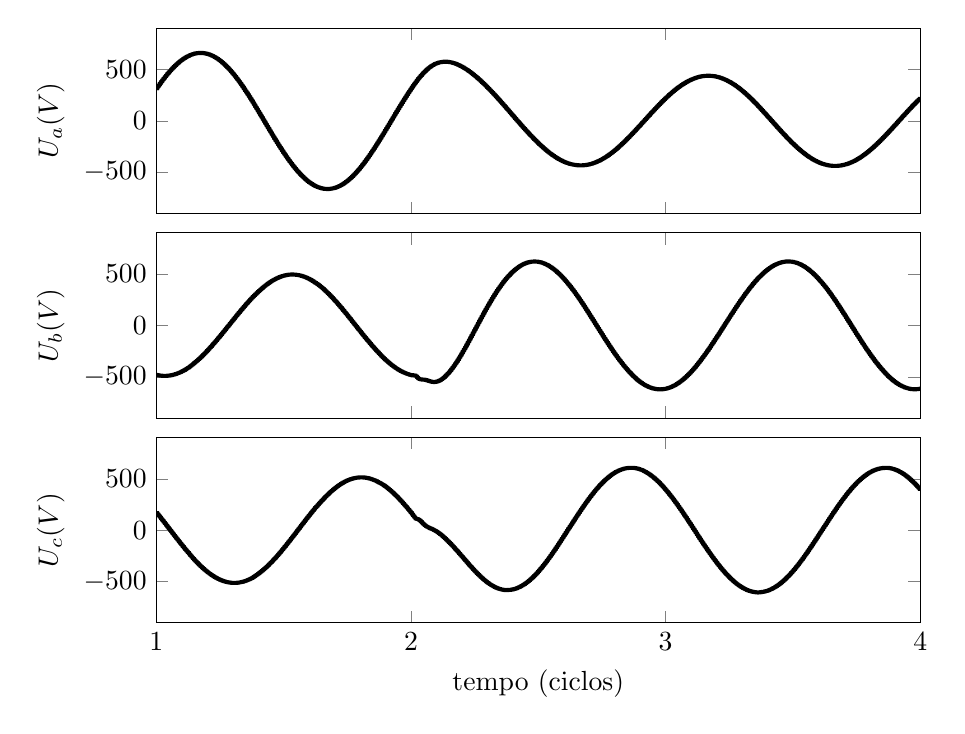
\begin{tikzpicture}

\begin{axis}[%
width=0.8\textwidth,
height=0.193917089240149\textwidth,
scale only axis,
xmin=0.0166666666666667,
xmax=0.0666666666666667,
xtick={0,0.0166666666666667,0.0333333333333333,0.05,0.0666666666666667},
xticklabels={\empty},
ymin=-900,
ymax=900,
ytick={-500,    0,  500},
ylabel={$\text{U}_\text{b}\text{ (V)}$},
name=plot2,
scaled x ticks = false,
legend columns=-1,
legend style={/tikz/every even column/.append style={column sep=0.3cm}},
legend style={font=\footnotesize}
]
\addplot [color=black,solid,line width=1.5pt,forget plot]
  table[row sep=crcr]{0.0166583333333333	-478.328989103039\\
0.0167	-481.372762295986\\
0.0167416666666667	-481.372762295986\\
0.0167833333333333	-483.944387417357\\
0.016825	-483.944387417357\\
0.0168666666666667	-486.043904769891\\
0.0169083333333333	-486.043904769891\\
0.01695	-487.669342075457\\
0.0169916666666667	-487.669342075457\\
0.0170333333333333	-488.81912329053\\
0.017075	-488.81912329053\\
0.0171166666666667	-489.492376222951\\
0.0171583333333333	-489.492376222951\\
0.0172	-489.689089295181\\
0.0172416666666667	-489.689089295181\\
0.0172833333333333	-489.410057478733\\
0.017325	-489.410057478733\\
0.0173666666666667	-488.656714544629\\
0.0174083333333333	-488.656714544629\\
0.01745	-487.430933830334\\
0.0174916666666667	-487.430933830334\\
0.0175333333333333	-485.734862735459\\
0.017575	-485.734862735459\\
0.0176166666666667	-483.570824107468\\
0.0176583333333333	-483.570824107468\\
0.0177	-480.941176730971\\
0.0177416666666667	-480.941176730971\\
0.0177833333333333	-477.848873406491\\
0.017825	-477.848873406491\\
0.0178666666666667	-474.296687037085\\
0.0179083333333333	-474.296687037085\\
0.01795	-470.287554266504\\
0.0179916666666667	-470.287554266504\\
0.0180333333333333	-465.824994538518\\
0.018075	-465.824994538518\\
0.0181166666666667	-460.912896166831\\
0.0181583333333333	-460.912896166831\\
0.0182	-455.555544349316\\
0.0182416666666667	-455.555544349316\\
0.0182833333333333	-449.757632700212\\
0.018325	-449.757632700212\\
0.0183666666666667	-443.524266807923\\
0.0184083333333333	-443.524266807923\\
0.01845	-436.860963041735\\
0.0184916666666667	-436.860963041735\\
0.0185333333333333	-429.773645406549\\
0.018575	-429.773645406549\\
0.0186166666666667	-422.2686421737\\
0.0186583333333333	-422.2686421737\\
0.0187	-414.352682994809\\
0.0187416666666667	-414.352682994809\\
0.0187833333333333	-406.710604021129\\
0.018825	-406.710604021129\\
0.0188666666666667	-396.968651829484\\
0.0189083333333333	-396.968651829484\\
0.01895	-387.24430030011\\
0.0189916666666667	-387.24430030011\\
0.0190333333333333	-377.413842111121\\
0.019075	-377.413842111121\\
0.0191166666666667	-367.3960735467\\
0.0191583333333333	-367.3960735467\\
0.0192	-357.12553953726\\
0.0192416666666667	-357.12553953726\\
0.0192833333333333	-346.559303382721\\
0.019325	-346.559303382721\\
0.0193666666666667	-335.674936708767\\
0.0194083333333333	-335.674936708767\\
0.01945	-324.465686057335\\
0.0194916666666667	-324.465686057335\\
0.0195333333333333	-312.935239244225\\
0.019575	-312.935239244225\\
0.0196166666666667	-301.093266862382\\
0.0196583333333333	-301.093266862382\\
0.0197	-288.95219973374\\
0.0197416666666667	-288.95219973374\\
0.0197833333333333	-276.525463982029\\
0.019825	-276.525463982029\\
0.0198666666666667	-263.82538033546\\
0.0199083333333333	-263.82538033546\\
0.01995	-250.865057706918\\
0.0199916666666667	-250.865057706918\\
0.0200333333333333	-237.656697428642\\
0.020075	-237.656697428642\\
0.0201166666666667	-224.212271375033\\
0.0201583333333333	-224.212271375033\\
0.0202	-210.543848998092\\
0.0202416666666667	-210.543848998092\\
0.0202833333333333	-196.6637735981\\
0.020325	-196.6637735981\\
0.0203666666666667	-182.584756063204\\
0.0204083333333333	-182.584756063204\\
0.02045	-168.319897946886\\
0.0204916666666667	-168.319897946886\\
0.0205333333333333	-153.882668002172\\
0.020575	-153.882668002172\\
0.0206166666666667	-139.286855686717\\
0.0206583333333333	-139.286855686717\\
0.0207	-124.546519243168\\
0.0207416666666667	-124.546519243168\\
0.0207833333333333	-109.675923407492\\
0.020825	-109.675923407492\\
0.0208666666666667	-94.6884951690301\\
0.0209083333333333	-94.6884951690301\\
0.02095	-79.6023211852309\\
0.0209916666666667	-79.6023211852309\\
0.0210333333333333	-64.4296541414652\\
0.021075	-64.4296541414652\\
0.0211166666666667	-49.1854677870168\\
0.0211583333333333	-49.1854677870168\\
0.0212	-33.8847697005379\\
0.0212416666666667	-33.8847697005379\\
0.0212833333333333	-18.5423320716325\\
0.021325	-18.5423320716325\\
0.0213666666666667	-3.1725945533516\\
0.0214083333333333	-3.1725945533516\\
0.02145	12.2102617721841\\
0.0214916666666667	12.2102617721841\\
0.0215333333333333	27.5921432856442\\
0.021575	27.5921432856442\\
0.0216166666666667	42.9588704890498\\
0.0216583333333333	42.9588704890498\\
0.0217	58.2960537853681\\
0.0217416666666667	58.2960537853681\\
0.0217833333333333	73.5890384864759\\
0.021825	73.5890384864759\\
0.0218666666666667	88.82269659409\\
0.0219083333333333	88.82269659409\\
0.02195	103.982669291038\\
0.0219916666666667	103.982669291038\\
0.0220333333333333	119.053037141893\\
0.022075	119.053037141893\\
0.0221166666666667	134.01853586672\\
0.0221583333333333	134.01853586672\\
0.0222	148.863909368128\\
0.0222416666666667	148.863909368128\\
0.0222833333333333	163.573956427556\\
0.022325	163.573956427556\\
0.0223666666666667	178.133568427636\\
0.0224083333333333	178.133568427636\\
0.02245	192.527757716713\\
0.0224916666666667	192.527757716713\\
0.0225333333333333	206.741679404245\\
0.022575	206.741679404245\\
0.0226166666666667	220.760649670751\\
0.0226583333333333	220.760649670751\\
0.0227	234.570162946369\\
0.0227416666666667	234.570162946369\\
0.0227833333333333	248.155909263895\\
0.022825	248.155909263895\\
0.0228666666666667	261.687830320942\\
0.0229083333333333	261.687830320942\\
0.02295	274.986604079196\\
0.0229916666666667	274.986604079196\\
0.0230333333333333	286.928801747272\\
0.023075	286.928801747272\\
0.0231166666666667	298.950506950644\\
0.0231583333333333	298.950506950644\\
0.0232	310.924864102034\\
0.0232416666666667	310.924864102034\\
0.0232833333333333	322.756989832147\\
0.023325	322.756989832147\\
0.0233666666666667	334.367084014297\\
0.0234083333333333	334.367084014297\\
0.02345	345.69602196514\\
0.0234916666666667	345.69602196514\\
0.0235333333333333	356.703461032175\\
0.023575	356.703461032175\\
0.0236166666666667	367.363371170442\\
0.0236583333333333	367.363371170442\\
0.0237	377.659204280424\\
0.0237416666666667	377.659204280424\\
0.0237833333333333	387.579795487262\\
0.023825	387.579795487262\\
0.0238666666666667	397.116425283701\\
0.0239083333333333	397.116425283701\\
0.02395	406.261310362139\\
0.0239916666666667	406.261310362139\\
0.0240333333333333	415.0053223807\\
0.024075	415.0053223807\\
0.0241166666666667	423.340732147141\\
0.0241583333333333	423.340732147141\\
0.0242	431.258683016742\\
0.0242416666666667	431.258683016742\\
0.0242833333333333	438.750365395371\\
0.024325	438.750365395371\\
0.0243666666666667	445.807262831054\\
0.0244083333333333	445.807262831054\\
0.02445	452.421342397773\\
0.0244916666666667	452.421342397773\\
0.0245333333333333	458.585161293933\\
0.024575	458.585161293933\\
0.0246166666666667	464.291905294308\\
0.0246583333333333	464.291905294308\\
0.0247	469.535383109734\\
0.0247416666666667	469.535383109734\\
0.0247833333333333	474.309999446141\\
0.024825	474.309999446141\\
0.0248666666666667	478.610723480444\\
0.0249083333333333	478.610723480444\\
0.02495	482.432523836755\\
0.0249916666666667	482.432523836755\\
0.0250333333333333	485.772612186125\\
0.025075	485.772612186125\\
0.0251166666666667	488.627883686145\\
0.0251583333333333	488.627883686145\\
0.0252	490.994391489966\\
0.0252416666666667	490.994391489966\\
0.0252833333333333	492.869784189106\\
0.025325	492.869784189106\\
0.0253666666666667	494.252063559781\\
0.0254083333333333	494.252063559781\\
0.02545	495.139387583695\\
0.0254916666666667	495.139387583695\\
0.0255333333333333	495.530061759552\\
0.025575	495.530061759552\\
0.0256166666666667	495.422663936061\\
0.0256583333333333	495.422663936061\\
0.0257	494.816230581684\\
0.0257416666666667	494.816230581684\\
0.0257833333333333	493.710425995119\\
0.025825	493.710425995119\\
0.0258666666666667	492.105654148384\\
0.0259083333333333	492.105654148384\\
0.02595	490.003108134894\\
0.0259916666666667	490.003108134894\\
0.0260333333333333	487.404961487327\\
0.026075	487.404961487327\\
0.0261166666666667	484.313069214194\\
0.0261583333333333	484.313069214194\\
0.0262	480.731558886196\\
0.0262416666666667	480.731558886196\\
0.0262833333333333	476.664323712434\\
0.026325	476.664323712434\\
0.0263666666666667	472.115829454631\\
0.0264083333333333	472.115829454631\\
0.02645	467.091068733291\\
0.0264916666666667	467.091068733291\\
0.0265333333333333	461.595540479995\\
0.026575	461.595540479995\\
0.0266166666666667	455.635234907076\\
0.0266583333333333	455.635234907076\\
0.0267	449.21662231492\\
0.0267416666666667	449.21662231492\\
0.0267833333333333	442.346643428456\\
0.026825	442.346643428456\\
0.0268666666666667	435.032699614098\\
0.0269083333333333	435.032699614098\\
0.02695	427.282642172915\\
0.0269916666666667	427.282642172915\\
0.0270333333333333	418.527982244731\\
0.027075	418.527982244731\\
0.0271166666666667	410.672570182659\\
0.0271583333333333	410.672570182659\\
0.0272	402.276872290978\\
0.0272416666666667	402.276872290978\\
0.0272833333333333	393.223850223727\\
0.027325	393.223850223727\\
0.0273666666666667	383.609151155178\\
0.0274083333333333	383.609151155178\\
0.02745	373.508718653929\\
0.0274916666666667	373.508718653929\\
0.0275333333333333	362.979579538073\\
0.027575	362.979579538073\\
0.0276166666666667	352.061894709897\\
0.0276583333333333	352.061894709897\\
0.0277	340.783205444461\\
0.0277416666666667	340.783205444461\\
0.0277833333333333	329.162781541968\\
0.027825	329.162781541968\\
0.0278666666666667	317.215226351439\\
0.0279083333333333	317.215226351439\\
0.02795	304.953068995059\\
0.0279916666666667	304.953068995059\\
0.0280333333333333	292.388308765939\\
0.028075	292.388308765939\\
0.0281166666666667	279.533394256386\\
0.0281583333333333	279.533394256386\\
0.0282	266.401997020689\\
0.0282416666666667	266.401997020689\\
0.0282833333333333	253.007121767018\\
0.028325	253.007121767018\\
0.0283666666666667	239.363037342399\\
0.0284083333333333	239.363037342399\\
0.02845	225.484309796947\\
0.0284916666666667	225.484309796947\\
0.0285333333333333	211.385672071801\\
0.028575	211.385672071801\\
0.0286166666666667	197.081935254737\\
0.0286583333333333	197.081935254737\\
0.0287	182.587950486431\\
0.0287416666666667	182.587950486431\\
0.0287833333333333	167.918604082923\\
0.028825	167.918604082923\\
0.0288666666666667	153.088829011011\\
0.0289083333333333	153.088829011011\\
0.02895	138.113619934855\\
0.0289916666666667	138.113619934855\\
0.0290333333333333	123.008044204917\\
0.029075	123.008044204917\\
0.0291166666666667	107.788100944899\\
0.0291583333333333	107.788100944899\\
0.0292	92.4664220892656\\
0.0292416666666667	92.4664220892656\\
0.0292833333333333	77.0599110293703\\
0.029325	77.0599110293703\\
0.0293666666666667	61.5839402726698\\
0.0294083333333333	61.5839402726698\\
0.02945	46.0538191073489\\
0.0294916666666667	46.0538191073489\\
0.0295333333333333	30.4851141949034\\
0.029575	30.4851141949034\\
0.0296166666666667	14.8937682112207\\
0.0296583333333333	14.8937682112207\\
0.0297	-0.703957306529608\\
0.0297416666666667	-0.703957306529608\\
0.0297833333333333	-16.2916492298269\\
0.029825	-16.2916492298269\\
0.0298666666666667	-31.8529362123827\\
0.0299083333333333	-31.8529362123827\\
0.02995	-47.371649369948\\
0.0299916666666667	-47.371649369948\\
0.0300333333333333	-62.8319222299047\\
0.030075	-62.8319222299047\\
0.0301166666666667	-78.2183969102601\\
0.0301583333333333	-78.2183969102601\\
0.0302	-93.5154108314719\\
0.0302416666666667	-93.5154108314719\\
0.0302833333333333	-108.70816278091\\
0.030325	-108.70816278091\\
0.0303666666666667	-123.782356080195\\
0.0304083333333333	-123.782356080195\\
0.03045	-138.723507249364\\
0.0304916666666667	-138.723507249364\\
0.0305333333333333	-153.517339096442\\
0.030575	-153.517339096442\\
0.0306166666666667	-168.149764544084\\
0.0306583333333333	-168.149764544084\\
0.0307	-182.60688669631\\
0.0307416666666667	-182.60688669631\\
0.0307833333333333	-196.875004412733\\
0.030825	-196.875004412733\\
0.0308666666666667	-210.940621254231\\
0.0309083333333333	-210.940621254231\\
0.03095	-224.790455634942\\
0.0309916666666667	-224.790455634942\\
0.0310333333333333	-238.411450801645\\
0.031075	-238.411450801645\\
0.0311166666666667	-251.788204920739\\
0.0311583333333333	-251.788204920739\\
0.0312	-264.319493294975\\
0.0312416666666667	-264.319493294975\\
0.0312833333333333	-278.081845363642\\
0.031325	-278.081845363642\\
0.0313666666666667	-291.211888263673\\
0.0314083333333333	-291.211888263673\\
0.03145	-303.807007713181\\
0.0314916666666667	-303.807007713181\\
0.0315333333333333	-315.936364357588\\
0.031575	-315.936364357588\\
0.0316166666666667	-327.655020751537\\
0.0316583333333333	-327.655020751537\\
0.0317	-338.998550237152\\
0.0317416666666667	-338.998550237152\\
0.0317833333333333	-349.984949605885\\
0.031825	-349.984949605885\\
0.0318666666666667	-360.618974262017\\
0.0319083333333333	-360.618974262017\\
0.03195	-370.896795074955\\
0.0319916666666667	-370.896795074955\\
0.0320333333333333	-380.809923421548\\
0.032075	-380.809923421548\\
0.0321166666666667	-390.348041070204\\
0.0321583333333333	-390.348041070204\\
0.0322	-399.500455565927\\
0.0322416666666667	-399.500455565927\\
0.0322833333333333	-408.258433783543\\
0.032325	-408.258433783543\\
0.0323666666666667	-416.612673979994\\
0.0324083333333333	-416.612673979994\\
0.03245	-424.555376388038\\
0.0324916666666667	-424.555376388038\\
0.0325333333333333	-432.079651399668\\
0.032575	-432.079651399668\\
0.0326166666666667	-439.17912856472\\
0.0326583333333333	-439.17912856472\\
0.0327	-445.847803165625\\
0.0327416666666667	-445.847803165625\\
0.0327833333333333	-452.079952433882\\
0.032825	-452.079952433882\\
0.0328666666666667	-457.870112681898\\
0.0329083333333333	-457.870112681898\\
0.03295	-463.213095942823\\
0.0329916666666667	-463.213095942823\\
0.0330333333333333	-468.104025539882\\
0.033075	-468.104025539882\\
0.0331166666666667	-472.538375275198\\
0.0331583333333333	-472.538375275198\\
0.0332	-476.512043591712\\
0.0332416666666667	-476.512043591712\\
0.0332833333333333	-480.021998518076\\
0.033325	-480.021998518076\\
0.0333666666666667	-483.062409528906\\
0.0334083333333333	-483.062409528906\\
0.03345	-483.678406180898\\
0.0334916666666667	-483.678406180898\\
0.0335333333333333	-485.862488721367\\
0.033575	-485.862488721367\\
0.0336166666666667	-488.142814475316\\
0.0336583333333333	-488.142814475316\\
0.0337	-498.245132388745\\
0.0337416666666667	-498.245132388745\\
0.0337833333333333	-510.177702028353\\
0.033825	-510.177702028353\\
0.0338666666666667	-518.869053971916\\
0.0339083333333333	-518.869053971916\\
0.03395	-523.323995836891\\
0.0339916666666667	-523.323995836891\\
0.0340333333333333	-524.949038961527\\
0.034075	-524.949038961527\\
0.0341166666666667	-525.669339355048\\
0.0341583333333333	-525.669339355048\\
0.0342	-526.908087285797\\
0.0342416666666667	-526.908087285797\\
0.0342833333333333	-529.296547986902\\
0.034325	-529.296547986902\\
0.0343666666666667	-532.790822709101\\
0.0344083333333333	-532.790822709101\\
0.03445	-536.931847441238\\
0.0344916666666667	-536.931847441238\\
0.0345333333333333	-541.107207956411\\
0.034575	-541.107207956411\\
0.0346166666666667	-544.736225800635\\
0.0346583333333333	-544.736225800635\\
0.0347	-547.369395078864\\
0.0347416666666667	-547.369395078864\\
0.0347833333333333	-548.716986912959\\
0.034825	-548.716986912959\\
0.0348666666666667	-548.632547118878\\
0.0349083333333333	-548.632547118878\\
0.03495	-547.075656823658\\
0.0349916666666667	-547.075656823658\\
0.0350333333333333	-544.071637409979\\
0.035075	-544.071637409979\\
0.0351166666666667	-539.678204260503\\
0.0351583333333333	-539.678204260503\\
0.0352	-533.962755583409\\
0.0352416666666667	-533.962755583409\\
0.0352833333333333	-527.182279910962\\
0.035325	-527.182279910962\\
0.0353666666666667	-519.113556680225\\
0.0354083333333333	-519.113556680225\\
0.03545	-509.000078841309\\
0.0354916666666667	-509.000078841309\\
0.0355333333333333	-498.107638282283\\
0.035575	-498.107638282283\\
0.0356166666666667	-486.375655173447\\
0.0356583333333333	-486.375655173447\\
0.0357	-473.759153944544\\
0.0357416666666667	-473.759153944544\\
0.0357833333333333	-460.236320033994\\
0.035825	-460.236320033994\\
0.0358666666666667	-445.810447327876\\
0.0359083333333333	-445.810447327876\\
0.03595	-430.505282665083\\
0.0359916666666667	-430.505282665083\\
0.0360333333333333	-414.358464568713\\
0.036075	-414.358464568713\\
0.0361166666666667	-397.415615024497\\
0.0361583333333333	-397.415615024497\\
0.0362	-379.725972742214\\
0.0362416666666667	-379.725972742214\\
0.0362833333333333	-361.339644418341\\
0.036325	-361.339644418341\\
0.0363666666666667	-342.306510620674\\
0.0364083333333333	-342.306510620674\\
0.03645	-322.673808653078\\
0.0364916666666667	-322.673808653078\\
0.0365333333333333	-302.490006690184\\
0.036575	-302.490006690184\\
0.0366166666666667	-281.801820654654\\
0.0366583333333333	-281.801820654654\\
0.0367	-260.65587850699\\
0.0367416666666667	-260.65587850699\\
0.0367833333333333	-239.098456719156\\
0.036825	-239.098456719156\\
0.0368666666666667	-217.175209420218\\
0.0369083333333333	-217.175209420218\\
0.03695	-194.931036851632\\
0.0369916666666667	-194.931036851632\\
0.0370333333333333	-172.410062075249\\
0.037075	-172.410062075249\\
0.0371166666666667	-149.655652803591\\
0.0371583333333333	-149.655652803591\\
0.0372	-126.710439524506\\
0.0372416666666667	-126.710439524506\\
0.0372833333333333	-103.616305295776\\
0.037325	-103.616305295776\\
0.0373666666666667	-80.4139546989703\\
0.0374083333333333	-80.4139546989703\\
0.03745	-57.1444016932104\\
0.0374916666666667	-57.1444016932104\\
0.0375333333333333	-33.8474272616072\\
0.037575	-33.8474272616072\\
0.0376166666666667	-10.5605046227431\\
0.0376583333333333	-10.5605046227431\\
0.0377	12.6791060967196\\
0.0377416666666667	12.6791060967196\\
0.0377833333333333	35.8353743740755\\
0.037825	35.8353743740755\\
0.0378666666666667	58.87364298905\\
0.0379083333333333	58.87364298905\\
0.03795	81.7608388535841\\
0.0379916666666667	81.7608388535841\\
0.0380333333333333	104.465378225758\\
0.038075	104.465378225758\\
0.0381166666666667	126.956956606797\\
0.0381583333333333	126.956956606797\\
0.0382	149.206353974694\\
0.0382416666666667	149.206353974694\\
0.0382833333333333	171.185317112742\\
0.038325	171.185317112742\\
0.0383666666666667	192.866498739553\\
0.0384083333333333	192.866498739553\\
0.03845	214.223301645853\\
0.0384916666666667	214.223301645853\\
0.0385333333333333	235.231350978712\\
0.038575	235.231350978712\\
0.0386166666666667	255.865244997372\\
0.0386583333333333	255.865244997372\\
0.0387	276.101702652239\\
0.0387416666666667	276.101702652239\\
0.0387833333333333	295.918476849333\\
0.038825	295.918476849333\\
0.0388666666666667	315.294326438433\\
0.0389083333333333	315.294326438433\\
0.03895	334.208995557844\\
0.0389916666666667	334.208995557844\\
0.0390333333333333	352.643192363139\\
0.039075	352.643192363139\\
0.0391166666666667	370.578568409044\\
0.0391583333333333	370.578568409044\\
0.0392	387.997699646167\\
0.0392416666666667	387.997699646167\\
0.0392833333333333	404.884069536479\\
0.039325	404.884069536479\\
0.0393666666666667	421.222054171729\\
0.0394083333333333	421.222054171729\\
0.03945	437.480424676999\\
0.0394916666666667	437.480424676999\\
0.0395333333333333	452.040941016559\\
0.039575	452.040941016559\\
0.0396166666666667	466.074182858891\\
0.0396583333333333	466.074182858891\\
0.0397	479.771235918754\\
0.0397416666666667	479.771235918754\\
0.0397833333333333	493.019679989615\\
0.039825	493.019679989615\\
0.0398666666666667	505.73413839378\\
0.0399083333333333	505.73413839378\\
0.03995	517.858623983074\\
0.0399916666666667	517.858623983074\\
0.0400333333333333	529.359563793907\\
0.040075	529.359563793907\\
0.0401166666666667	540.217966392563\\
0.0401583333333333	540.217966392563\\
0.0402	550.422720161551\\
0.0402416666666667	550.422720161551\\
0.0402833333333333	559.966764407743\\
0.040325	559.966764407743\\
0.0403666666666667	568.844782875507\\
0.0404083333333333	568.844782875507\\
0.04045	577.05210647663\\
0.0404916666666667	577.05210647663\\
0.0405333333333333	584.58398245434\\
0.040575	584.58398245434\\
0.0406166666666667	591.435324944241\\
0.0406583333333333	591.435324944241\\
0.0407	597.602956497375\\
0.0407416666666667	597.602956497375\\
0.0407833333333333	603.083411539344\\
0.040825	603.083411539344\\
0.0408666666666667	607.874065878715\\
0.0409083333333333	607.874065878715\\
0.04095	611.973246455818\\
0.0409916666666667	611.973246455818\\
0.0410333333333333	615.380238806002\\
0.041075	615.380238806002\\
0.0411166666666667	618.095240312968\\
0.0411583333333333	618.095240312968\\
0.0412	620.119289539734\\
0.0412416666666667	620.119289539734\\
0.0412833333333333	621.454193408118\\
0.041325	621.454193408118\\
0.0413666666666667	622.102464544814\\
0.0414083333333333	622.102464544814\\
0.04145	622.067273281086\\
0.0414916666666667	622.067273281086\\
0.0415333333333333	621.351782529469\\
0.041575	621.351782529469\\
0.0416166666666667	619.962242070563\\
0.0416583333333333	619.962242070563\\
0.0417	617.902615212395\\
0.0417416666666667	617.902615212395\\
0.0417833333333333	615.17835164608\\
0.041825	615.17835164608\\
0.0418666666666667	611.795572072393\\
0.0419083333333333	611.795572072393\\
0.04195	607.760754022874\\
0.0419916666666667	607.760754022874\\
0.0420333333333333	603.080607489372\\
0.042075	603.080607489372\\
0.0421166666666667	597.762108228377\\
0.0421583333333333	597.762108228377\\
0.0422	591.812622646619\\
0.0422416666666667	591.812622646619\\
0.0422833333333333	585.240054074818\\
0.042325	585.240054074818\\
0.0423666666666667	578.052948832242\\
0.0424083333333333	578.052948832242\\
0.04245	570.260538255211\\
0.0424916666666667	570.260538255211\\
0.0425333333333333	561.872936284205\\
0.042575	561.872936284205\\
0.0426166666666667	552.900083112745\\
0.0426583333333333	552.900083112745\\
0.0427	543.353207689846\\
0.0427416666666667	543.353207689846\\
0.0427833333333333	533.244433887195\\
0.042825	533.244433887195\\
0.0428666666666667	522.585826182198\\
0.0429083333333333	522.585826182198\\
0.04295	511.389933785599\\
0.0429916666666667	511.389933785599\\
0.0430333333333333	499.669787225859\\
0.043075	499.669787225859\\
0.0431166666666667	487.438882456456\\
0.0431583333333333	487.438882456456\\
0.0432	474.711164930049\\
0.0432416666666667	474.711164930049\\
0.0432833333333333	461.501013707399\\
0.043325	461.501013707399\\
0.0433666666666667	447.82322510983\\
0.0434083333333333	447.82322510983\\
0.04345	433.692995682403\\
0.0434916666666667	433.692995682403\\
0.0435333333333333	419.114123530008\\
0.043575	419.114123530008\\
0.0436166666666667	403.630299904557\\
0.0436583333333333	403.630299904557\\
0.0437	389.067248906318\\
0.0437416666666667	389.067248906318\\
0.0437833333333333	373.794607970039\\
0.043825	373.794607970039\\
0.0438666666666667	357.893910580944\\
0.0439083333333333	357.893910580944\\
0.04395	341.48847965027\\
0.0439916666666667	341.48847965027\\
0.0440333333333333	324.669814436674\\
0.044075	324.669814436674\\
0.0441166666666667	307.499399030616\\
0.0441583333333333	307.499399030616\\
0.0442	290.017043641092\\
0.0442416666666667	290.017043641092\\
0.0442833333333333	272.249315182523\\
0.044325	272.249315182523\\
0.0443666666666667	254.216038867438\\
0.0444083333333333	254.216038867438\\
0.04445	235.934592114668\\
0.0444916666666667	235.934592114668\\
0.0445333333333333	217.422270956511\\
0.044575	217.422270956511\\
0.0446166666666667	198.696939122818\\
0.0446583333333333	198.696939122818\\
0.0447	179.778898467287\\
0.0447416666666667	179.778898467287\\
0.0447833333333333	160.687408623789\\
0.044825	160.687408623789\\
0.0448666666666667	141.442715029629\\
0.0449083333333333	141.442715029629\\
0.04495	122.065482129781\\
0.0449916666666667	122.065482129781\\
0.0450333333333333	102.576274992799\\
0.045075	102.576274992799\\
0.0451166666666667	82.9954553821085\\
0.0451583333333333	82.9954553821085\\
0.0452	63.3431668052044\\
0.0452416666666667	63.3431668052044\\
0.0452833333333333	43.6393638336056\\
0.045325	43.6393638336056\\
0.0453666666666667	23.9038552313563\\
0.0454083333333333	23.9038552313563\\
0.04545	4.15634192700959\\
0.0454916666666667	4.15634192700959\\
0.0455333333333333	-15.5835589467395\\
0.045575	-15.5835589467395\\
0.0456166666666667	-35.2962607915949\\
0.0456583333333333	-35.2962607915949\\
0.0457	-54.9618164960153\\
0.0457416666666667	-54.9618164960153\\
0.0457833333333333	-74.5626887768094\\
0.045825	-74.5626887768094\\
0.0458666666666667	-94.0783942026847\\
0.0459083333333333	-94.0783942026847\\
0.04595	-113.489817630002\\
0.0459916666666667	-113.489817630002\\
0.0460333333333333	-132.777948092905\\
0.046075	-132.777948092905\\
0.0461166666666667	-151.923684718905\\
0.0461583333333333	-151.923684718905\\
0.0462	-170.907795748521\\
0.0462416666666667	-170.907795748521\\
0.0462833333333333	-189.711018370974\\
0.046325	-189.711018370974\\
0.0463666666666667	-208.314223883074\\
0.0464083333333333	-208.314223883074\\
0.04645	-226.69857913687\\
0.0464916666666667	-226.69857913687\\
0.0465333333333333	-244.845655884747\\
0.046575	-244.845655884747\\
0.0466166666666667	-262.73747467731\\
0.0466583333333333	-262.73747467731\\
0.0467	-280.35685709118\\
0.0467416666666667	-280.35685709118\\
0.0467833333333333	-297.685436154517\\
0.046825	-297.685436154517\\
0.0468666666666667	-314.707570290364\\
0.0469083333333333	-314.707570290364\\
0.04695	-331.406944088127\\
0.0469916666666667	-331.406944088127\\
0.0470333333333333	-347.767508096617\\
0.047075	-347.767508096617\\
0.0471166666666667	-363.773616624145\\
0.0471583333333333	-363.773616624145\\
0.0472	-379.410038002404\\
0.0472416666666667	-379.410038002404\\
0.0472833333333333	-394.661961827583\\
0.047325	-394.661961827583\\
0.0473666666666667	-409.515006542937\\
0.0474083333333333	-409.515006542937\\
0.04745	-423.955227040306\\
0.0474916666666667	-423.955227040306\\
0.0475333333333333	-437.96912175223\\
0.047575	-437.96912175223\\
0.0476166666666667	-451.543639085691\\
0.0476583333333333	-451.543639085691\\
0.0477	-464.479544997007\\
0.0477416666666667	-464.479544997007\\
0.0477833333333333	-477.089008664143\\
0.047825	-477.089008664143\\
0.0478666666666667	-489.980276495137\\
0.0479083333333333	-489.980276495137\\
0.04795	-502.082454983243\\
0.0479916666666667	-502.082454983243\\
0.0480333333333333	-513.474378594949\\
0.048075	-513.474378594949\\
0.0481166666666667	-524.236448612188\\
0.0481583333333333	-524.236448612188\\
0.0482	-534.419855442406\\
0.0482416666666667	-534.419855442406\\
0.0482833333333333	-544.05048530493\\
0.048325	-544.05048530493\\
0.0483666666666667	-553.136657143756\\
0.0484083333333333	-553.136657143756\\
0.04845	-561.676386905996\\
0.0484916666666667	-561.676386905996\\
0.0485333333333333	-569.662827271978\\
0.048575	-569.662827271978\\
0.0486166666666667	-577.087697701991\\
0.0486583333333333	-577.087697701991\\
0.0487	-583.943144390163\\
0.0487416666666667	-583.943144390163\\
0.0487833333333333	-590.222145166835\\
0.048825	-590.222145166835\\
0.0488666666666667	-595.920726335499\\
0.0489083333333333	-595.920726335499\\
0.04895	-601.033307618998\\
0.0489916666666667	-601.033307618998\\
0.0490333333333333	-605.556420963213\\
0.049075	-605.556420963213\\
0.0491166666666667	-609.487177748175\\
0.0491583333333333	-609.487177748175\\
0.0492	-612.823052256476\\
0.0492416666666667	-612.823052256476\\
0.0492833333333333	-615.561826877812\\
0.049325	-615.561826877812\\
0.0493666666666667	-617.701607112424\\
0.0494083333333333	-617.701607112424\\
0.04945	-619.240871262007\\
0.0494916666666667	-619.240871262007\\
0.0495333333333333	-620.178528934764\\
0.049575	-620.178528934764\\
0.0496166666666667	-620.513972615137\\
0.0496583333333333	-620.513972615137\\
0.0497	-620.247115363624\\
0.0497416666666667	-620.247115363624\\
0.0497833333333333	-619.378688758982\\
0.049825	-619.378688758982\\
0.0498666666666667	-617.909223463945\\
0.0499083333333333	-617.909223463945\\
0.04995	-615.839755643643\\
0.0499916666666667	-615.839755643643\\
0.0500333333333333	-613.173045332849\\
0.050075	-613.173045332849\\
0.0501166666666667	-609.911750435669\\
0.0501583333333333	-609.911750435669\\
0.0502	-606.059195153575\\
0.0502416666666667	-606.059195153575\\
0.0502833333333333	-601.619528288722\\
0.050325	-601.619528288722\\
0.0503666666666667	-596.5977218648\\
0.0504083333333333	-596.5977218648\\
0.05045	-590.999459574474\\
0.0504916666666667	-590.999459574474\\
0.0505333333333333	-584.830984389048\\
0.050575	-584.830984389048\\
0.0506166666666667	-578.098972885875\\
0.0506583333333333	-578.098972885875\\
0.0507	-570.810458695109\\
0.0507416666666667	-570.810458695109\\
0.0507833333333333	-562.972771453032\\
0.050825	-562.972771453032\\
0.0508666666666667	-554.593458705033\\
0.0509083333333333	-554.593458705033\\
0.05095	-545.681768487654\\
0.0509916666666667	-545.681768487654\\
0.0510333333333333	-536.245095988263\\
0.051075	-536.245095988263\\
0.0511166666666667	-526.292515885746\\
0.0511583333333333	-526.292515885746\\
0.0512	-515.83356953895\\
0.0512416666666667	-515.83356953895\\
0.0512833333333333	-504.878224034623\\
0.051325	-504.878224034623\\
0.0513666666666667	-493.436867537464\\
0.0514083333333333	-493.436867537464\\
0.05145	-481.52030596022\\
0.0514916666666667	-481.52030596022\\
0.0515333333333333	-469.139759186227\\
0.051575	-469.139759186227\\
0.0516166666666667	-456.306856819179\\
0.0516583333333333	-456.306856819179\\
0.0517	-443.033633642018\\
0.0517416666666667	-443.033633642018\\
0.0517833333333333	-429.33258029632\\
0.051825	-429.33258029632\\
0.0518666666666667	-415.631465352924\\
0.0519083333333333	-415.631465352924\\
0.05195	-400.572255393978\\
0.0519916666666667	-400.572255393978\\
0.0520333333333333	-385.137617929011\\
0.052075	-385.137617929011\\
0.0521166666666667	-369.577327567763\\
0.0521583333333333	-369.577327567763\\
0.0522	-353.811156353638\\
0.0522416666666667	-353.811156353638\\
0.0522833333333333	-337.782144292742\\
0.052325	-337.782144292742\\
0.0523666666666667	-321.461774745628\\
0.0524083333333333	-321.461774745628\\
0.05245	-304.842729371899\\
0.0524916666666667	-304.842729371899\\
0.0525333333333333	-287.93107573415\\
0.052575	-287.93107573415\\
0.0526166666666667	-270.740138534588\\
0.0526583333333333	-270.740138534588\\
0.0527	-253.286428675406\\
0.0527416666666667	-253.286428675406\\
0.0527833333333333	-235.587304265221\\
0.052825	-235.587304265221\\
0.0528666666666667	-217.660084870833\\
0.0529083333333333	-217.660084870833\\
0.05295	-199.521347520453\\
0.0529916666666667	-199.521347520453\\
0.0530333333333333	-181.186956202741\\
0.053075	-181.186956202741\\
0.0531166666666667	-162.674350682609\\
0.0531583333333333	-162.674350682609\\
0.0532	-144.000119294864\\
0.0532416666666667	-144.000119294864\\
0.0532833333333333	-125.181189054423\\
0.053325	-125.181189054423\\
0.0533666666666667	-106.234904649345\\
0.0534083333333333	-106.234904649345\\
0.05345	-87.1790079525377\\
0.0534916666666667	-87.1790079525377\\
0.0535333333333333	-68.0315757914698\\
0.053575	-68.0315757914698\\
0.0536166666666667	-48.8109448712189\\
0.0536583333333333	-48.8109448712189\\
0.0537	-29.535641501431\\
0.0537416666666667	-29.535641501431\\
0.0537833333333333	-10.2243242585009\\
0.053825	-10.2243242585009\\
0.0538666666666667	9.10425939312514\\
0.0539083333333333	9.10425939312514\\
0.05395	28.431759765239\\
0.0539916666666667	28.431759765239\\
0.0540333333333333	47.7380619914277\\
0.054075	47.7380619914277\\
0.0541166666666667	67.0048596216789\\
0.0541583333333333	67.0048596216789\\
0.0542	86.2134287761061\\
0.0542416666666667	86.2134287761061\\
0.0542833333333333	105.344932703909\\
0.054325	105.344932703909\\
0.0543666666666667	124.380749221213\\
0.0544083333333333	124.380749221213\\
0.05445	143.302595289061\\
0.0544916666666667	143.302595289061\\
0.0545333333333333	162.092504174167\\
0.054575	162.092504174167\\
0.0546166666666667	180.732720410386\\
0.0546583333333333	180.732720410386\\
0.0547	199.205581326043\\
0.0547416666666667	199.205581326043\\
0.0547833333333333	217.493428750765\\
0.054825	217.493428750765\\
0.0548666666666667	235.578582767079\\
0.0549083333333333	235.578582767079\\
0.05495	253.443125065313\\
0.0549916666666667	253.443125065313\\
0.0550333333333333	271.070114062267\\
0.055075	271.070114062267\\
0.0551166666666667	288.441918437565\\
0.0551583333333333	288.441918437565\\
0.0552	305.540629346178\\
0.0552416666666667	305.540629346178\\
0.0552833333333333	322.349196138942\\
0.055325	322.349196138942\\
0.0553666666666667	338.850790392749\\
0.0554083333333333	338.850790392749\\
0.05545	355.028813235841\\
0.0554916666666667	355.028813235841\\
0.0555333333333333	370.866918292704\\
0.055575	370.866918292704\\
0.0556166666666667	386.349034907237\\
0.0556583333333333	386.349034907237\\
0.0557	401.459390824441\\
0.0557416666666667	401.459390824441\\
0.0557833333333333	416.182534509225\\
0.055825	416.182534509225\\
0.0558666666666667	430.503357233046\\
0.0559083333333333	430.503357233046\\
0.05595	444.428364259702\\
0.0559916666666667	444.428364259702\\
0.0560333333333333	458.312095926699\\
0.056075	458.312095926699\\
0.0561166666666667	470.620831923049\\
0.0561583333333333	470.620831923049\\
0.0562	482.740252403833\\
0.0562416666666667	482.740252403833\\
0.0562833333333333	494.614442650844\\
0.056325	494.614442650844\\
0.0563666666666667	506.137452019097\\
0.0564083333333333	506.137452019097\\
0.05645	517.232035261074\\
0.0564916666666667	517.232035261074\\
0.0565333333333333	527.848037766364\\
0.056575	527.848037766364\\
0.0566166666666667	537.955006311181\\
0.0566583333333333	537.955006311181\\
0.0567	547.534799837882\\
0.0567416666666667	547.534799837882\\
0.0567833333333333	556.575910547173\\
0.056825	556.575910547173\\
0.0568666666666667	565.069730447462\\
0.0569083333333333	565.069730447462\\
0.05695	573.008501865003\\
0.0569916666666667	573.008501865003\\
0.0570333333333333	580.384800104896\\
0.057075	580.384800104896\\
0.0571166666666667	587.189514084658\\
0.0571583333333333	587.189514084658\\
0.0572	593.415496031393\\
0.0572416666666667	593.415496031393\\
0.0572833333333333	599.055415177099\\
0.057325	599.055415177099\\
0.0573666666666667	604.102157217934\\
0.0574083333333333	604.102157217934\\
0.05745	608.549383427174\\
0.0574916666666667	608.549383427174\\
0.0575333333333333	612.391612312246\\
0.057575	612.391612312246\\
0.0576166666666667	615.624219432025\\
0.0576583333333333	615.624219432025\\
0.0577	618.243397323232\\
0.0577416666666667	618.243397323232\\
0.0577833333333333	620.246102846652\\
0.057825	620.246102846652\\
0.0578666666666667	621.630008937807\\
0.0579083333333333	621.630008937807\\
0.05795	622.393468628273\\
0.0579916666666667	622.393468628273\\
0.0580333333333333	622.535455960628\\
0.058075	622.535455960628\\
0.0581166666666667	622.055271597177\\
0.0581583333333333	622.055271597177\\
0.0582	620.954537902664\\
0.0582416666666667	620.954537902664\\
0.0582833333333333	619.2334104644\\
0.058325	619.2334104644\\
0.0583666666666667	616.893467377475\\
0.0584083333333333	616.893467377475\\
0.05845	613.936896430051\\
0.0584916666666667	613.936896430051\\
0.0585333333333333	610.36630880557\\
0.058575	610.36630880557\\
0.0586166666666667	606.18468480805\\
0.0586583333333333	606.18468480805\\
0.0587	601.395442675433\\
0.0587416666666667	601.395442675433\\
0.0587833333333333	596.002565110854\\
0.058825	596.002565110854\\
0.0588666666666667	590.010720188448\\
0.0589083333333333	590.010720188448\\
0.05895	583.4253374101\\
0.0589916666666667	583.4253374101\\
0.0590333333333333	576.252628904655\\
0.059075	576.252628904655\\
0.0591166666666667	568.499948956247\\
0.0591583333333333	568.499948956247\\
0.0592	560.173614212181\\
0.0592416666666667	560.173614212181\\
0.0592833333333333	551.28312413464\\
0.059325	551.28312413464\\
0.0593666666666667	541.837523603996\\
0.0594083333333333	541.837523603996\\
0.05945	531.84630593606\\
0.0594916666666667	531.84630593606\\
0.0595333333333333	521.319576753576\\
0.059575	521.319576753576\\
0.0596166666666667	510.268040036644\\
0.0596583333333333	510.268040036644\\
0.0597	498.702979267305\\
0.0597416666666667	498.702979267305\\
0.0597833333333333	486.636238742145\\
0.059825	486.636238742145\\
0.0598666666666667	474.080205128796\\
0.0599083333333333	474.080205128796\\
0.05995	461.047788826581\\
0.0599916666666667	461.047788826581\\
0.0600333333333333	447.552404921158\\
0.060075	447.552404921158\\
0.0601166666666667	433.432158149113\\
0.0601583333333333	433.432158149113\\
0.0602	419.033196012895\\
0.0602416666666667	419.033196012895\\
0.0602833333333333	404.859615019062\\
0.060325	404.859615019062\\
0.0603666666666667	390.014032323058\\
0.0604083333333333	390.014032323058\\
0.06045	374.591154785734\\
0.0604916666666667	374.591154785734\\
0.0605333333333333	358.687629768179\\
0.060575	358.687629768179\\
0.0606166666666667	342.37391082923\\
0.0606583333333333	342.37391082923\\
0.0607	325.697776804887\\
0.0607416666666667	325.697776804887\\
0.0607833333333333	308.691270197785\\
0.060825	308.691270197785\\
0.0608666666666667	291.377167396606\\
0.0609083333333333	291.377167396606\\
0.06095	273.773785867276\\
0.0609916666666667	273.773785867276\\
0.0610333333333333	255.898042095002\\
0.061075	255.898042095002\\
0.0611166666666667	237.767089849261\\
0.0611583333333333	237.767089849261\\
0.0612	219.398595908806\\
0.0612416666666667	219.398595908806\\
0.0612833333333333	200.812941399026\\
0.061325	200.812941399026\\
0.0613666666666667	182.028311218103\\
0.0614083333333333	182.028311218103\\
0.06145	163.064650695835\\
0.0614916666666667	163.064650695835\\
0.0615333333333333	143.94210388579\\
0.061575	143.94210388579\\
0.0616166666666667	124.680771383585\\
0.0616583333333333	124.680771383585\\
0.0617	105.300645415707\\
0.0617416666666667	105.300645415707\\
0.0617833333333333	85.8216061912758\\
0.061825	85.8216061912758\\
0.0618666666666667	66.2634467052476\\
0.0619083333333333	66.2634467052476\\
0.06195	46.6459034390845\\
0.0619916666666667	46.6459034390845\\
0.0620333333333333	26.9886799274167\\
0.062075	26.9886799274167\\
0.0621166666666667	7.31145794450646\\
0.0621583333333333	7.31145794450646\\
0.0622	-12.3659182597896\\
0.0622416666666667	-12.3659182597896\\
0.0622833333333333	-32.0240741012994\\
0.062325	-32.0240741012994\\
0.0623666666666667	-51.6439831541824\\
0.0624083333333333	-51.6439831541824\\
0.06245	-71.2056745782734\\
0.0624916666666667	-71.2056745782734\\
0.0625333333333333	-90.6897327387127\\
0.062575	-90.6897327387127\\
0.0626166666666667	-110.076751617406\\
0.0626583333333333	-110.076751617406\\
0.0627	-129.347213340142\\
0.0627416666666667	-129.347213340142\\
0.0627833333333333	-148.481504179948\\
0.062825	-148.481504179948\\
0.0628666666666667	-167.460028032437\\
0.0629083333333333	-167.460028032437\\
0.06295	-186.263355478126\\
0.0629916666666667	-186.263355478126\\
0.0630333333333333	-204.872350936187\\
0.063075	-204.872350936187\\
0.0631166666666667	-223.268246970837\\
0.0631583333333333	-223.268246970837\\
0.0632	-241.432738266829\\
0.0632416666666667	-241.432738266829\\
0.0632833333333333	-259.34798799135\\
0.063325	-259.34798799135\\
0.0633666666666667	-276.995243523329\\
0.0634083333333333	-276.995243523329\\
0.06345	-294.358484838227\\
0.0634916666666667	-294.358484838227\\
0.0635333333333333	-311.42072943262\\
0.063575	-311.42072943262\\
0.0636166666666667	-328.165320103536\\
0.0636583333333333	-328.165320103536\\
0.0637	-344.57598586431\\
0.0637416666666667	-344.57598586431\\
0.0637833333333333	-360.636853066169\\
0.063825	-360.636853066169\\
0.0638666666666667	-376.332453468804\\
0.0639083333333333	-376.332453468804\\
0.06395	-391.647731942395\\
0.0639916666666667	-391.647731942395\\
0.0640333333333333	-406.568054117199\\
0.064075	-406.568054117199\\
0.0641166666666667	-421.079213855563\\
0.0641583333333333	-421.079213855563\\
0.0642	-435.166921635444\\
0.0642416666666667	-435.166921635444\\
0.0642833333333333	-448.461112459469\\
0.064325	-448.461112459469\\
0.0643666666666667	-462.122406471931\\
0.0644083333333333	-462.122406471931\\
0.06445	-475.340031263127\\
0.0644916666666667	-475.340031263127\\
0.0645333333333333	-487.859730932864\\
0.064575	-487.859730932864\\
0.0646166666666667	-499.754576781684\\
0.0646583333333333	-499.754576781684\\
0.0647	-511.078436924127\\
0.0647416666666667	-511.078436924127\\
0.0647833333333333	-521.860443670578\\
0.064825	-521.860443670578\\
0.0648666666666667	-532.111378784872\\
0.0649083333333333	-532.111378784872\\
0.06495	-541.830649152533\\
0.0649916666666667	-541.830649152533\\
0.0650333333333333	-551.011800488711\\
0.065075	-551.011800488711\\
0.0651166666666667	-559.646203309419\\
0.0651583333333333	-559.646203309419\\
0.0652	-567.725163321087\\
0.0652416666666667	-567.725163321087\\
0.0652833333333333	-575.24070632805\\
0.065325	-575.24070632805\\
0.0653666666666667	-582.186400097242\\
0.0654083333333333	-582.186400097242\\
0.06545	-588.557175167164\\
0.0654916666666667	-588.557175167164\\
0.0655333333333333	-594.34710859428\\
0.065575	-594.34710859428\\
0.0656166666666667	-599.551945853093\\
0.0656583333333333	-599.551945853093\\
0.0657	-604.167854859234\\
0.0657416666666667	-604.167854859234\\
0.0657833333333333	-608.191333491608\\
0.065825	-608.191333491608\\
0.0658666666666667	-611.619214958316\\
0.0659083333333333	-611.619214958316\\
0.06595	-614.448712059601\\
0.0659916666666667	-614.448712059601\\
0.0660333333333333	-616.677473478238\\
0.066075	-616.677473478238\\
0.0661166666666667	-618.303635491654\\
0.0661583333333333	-618.303635491654\\
0.0662	-619.325861244175\\
0.0662416666666667	-619.325861244175\\
0.0662833333333333	-619.743366064574\\
0.066325	-619.743366064574\\
0.0663666666666667	-619.55625036455\\
0.0664083333333333	-619.55625036455\\
0.06645	-618.764042238611\\
0.0664916666666667	-618.764042238611\\
0.0665333333333333	-617.367869927798\\
0.066575	-617.367869927798\\
0.0666166666666667	-615.369358265863\\
0.0666583333333333	-615.369358265863\\
};
\end{axis}

\begin{axis}[%
width=0.8\textwidth,
height=0.193917089240149\textwidth,
scale only axis,
xmin=0.0166666666666667,
xmax=0.0666666666666667,
xtick={0,0.0166666666666667,0.0333333333333333,0.05,0.0666666666666667},
xticklabels={{0},{1},{2},{3},{4}},
xlabel={tempo (ciclos)},
ymin=-900,
ymax=900,
ytick={-500,    0,  500},
ylabel={$\text{U}_\text{c}\text{ (V)}$},
at=(plot2.below south west),
anchor=above north west,
scaled x ticks = false,
legend columns=-1,
legend style={/tikz/every even column/.append style={column sep=0.3cm}},
legend style={font=\footnotesize}
]
\addplot [color=black,solid,line width=1.5pt,forget plot]
  table[row sep=crcr]{0.0166583333333333	180.146044285981\\
0.0167	164.940320934484\\
0.0167416666666667	164.940320934484\\
0.0167833333333333	149.579587477261\\
0.016825	149.579587477261\\
0.0168666666666667	134.079551509137\\
0.0169083333333333	134.079551509137\\
0.01695	118.455249604828\\
0.0169916666666667	118.455249604828\\
0.0170333333333333	102.721820759597\\
0.017075	102.721820759597\\
0.0171166666666667	86.8947024886041\\
0.0171583333333333	86.8947024886041\\
0.0172	70.9897152347551\\
0.0172416666666667	70.9897152347551\\
0.0172833333333333	55.0229884605968\\
0.017325	55.0229884605968\\
0.0173666666666667	39.0107951391398\\
0.0174083333333333	39.0107951391398\\
0.01745	22.9693692316446\\
0.0174916666666667	22.9693692316446\\
0.0175333333333333	6.91476165823279\\
0.017575	6.91476165823279\\
0.0176166666666667	-9.13724020053355\\
0.0176583333333333	-9.13724020053355\\
0.0177	-25.1712876244939\\
0.0177416666666667	-25.1712876244939\\
0.0177833333333333	-41.1717016099994\\
0.017825	-41.1717016099994\\
0.0178666666666667	-57.1235450619316\\
0.0179083333333333	-57.1235450619316\\
0.01795	-73.0122416753861\\
0.0179916666666667	-73.0122416753861\\
0.0180333333333333	-88.8229904086394\\
0.018075	-88.8229904086394\\
0.0181166666666667	-104.541092542183\\
0.0181583333333333	-104.541092542183\\
0.0182	-120.151937938219\\
0.0182416666666667	-120.151937938219\\
0.0182833333333333	-135.641005542097\\
0.018325	-135.641005542097\\
0.0183666666666667	-150.993870043721\\
0.0184083333333333	-150.993870043721\\
0.01845	-166.196212093992\\
0.0184916666666667	-166.196212093992\\
0.0185333333333333	-181.2338298443\\
0.018575	-181.2338298443\\
0.0186166666666667	-196.092650491087\\
0.0186583333333333	-196.092650491087\\
0.0187	-210.758741337919\\
0.0187416666666667	-210.758741337919\\
0.0187833333333333	-224.272823986116\\
0.018825	-224.272823986116\\
0.0188666666666667	-239.924185188171\\
0.0189083333333333	-239.924185188171\\
0.01895	-254.795099361687\\
0.0189916666666667	-254.795099361687\\
0.0190333333333333	-269.036557729883\\
0.019075	-269.036557729883\\
0.0191166666666667	-282.760389233867\\
0.0191583333333333	-282.760389233867\\
0.0192	-296.057851197266\\
0.0192416666666667	-296.057851197266\\
0.0192833333333333	-308.990098283122\\
0.019325	-308.990098283122\\
0.0193666666666667	-321.590393418407\\
0.0194083333333333	-321.590393418407\\
0.01945	-333.870571911174\\
0.0194916666666667	-333.870571911174\\
0.0195333333333333	-345.828322444006\\
0.019575	-345.828322444006\\
0.0196166666666667	-357.453508661192\\
0.0196583333333333	-357.453508661192\\
0.0197	-368.732790011102\\
0.0197416666666667	-368.732790011102\\
0.0197833333333333	-379.652185798579\\
0.019825	-379.652185798579\\
0.0198666666666667	-390.200039679523\\
0.0199083333333333	-390.200039679523\\
0.01995	-400.364455853375\\
0.0199916666666667	-400.364455853375\\
0.0200333333333333	-410.135593074462\\
0.020075	-410.135593074462\\
0.0201166666666667	-419.504723697965\\
0.0201583333333333	-419.504723697965\\
0.0202	-428.463752199279\\
0.0202416666666667	-428.463752199279\\
0.0202833333333333	-437.004944992871\\
0.020325	-437.004944992871\\
0.0203666666666667	-445.120779808899\\
0.0204083333333333	-445.120779808899\\
0.02045	-452.8038978512\\
0.0204916666666667	-452.8038978512\\
0.0205333333333333	-460.047124180064\\
0.020575	-460.047124180064\\
0.0206166666666667	-466.843522119401\\
0.0206583333333333	-466.843522119401\\
0.0207	-473.186455823302\\
0.0207416666666667	-473.186455823302\\
0.0207833333333333	-479.069643185327\\
0.020825	-479.069643185327\\
0.0208666666666667	-484.487584080736\\
0.0209083333333333	-484.487584080736\\
0.02095	-489.433644253288\\
0.0209916666666667	-489.433644253288\\
0.0210333333333333	-493.903539136153\\
0.021075	-493.903539136153\\
0.0211166666666667	-497.892633124744\\
0.0211583333333333	-497.892633124744\\
0.0212	-501.396820907034\\
0.0212416666666667	-501.396820907034\\
0.0212833333333333	-504.41270742765\\
0.021325	-504.41270742765\\
0.0213666666666667	-506.937652408911\\
0.0214083333333333	-506.937652408911\\
0.02145	-508.969679717527\\
0.0214916666666667	-508.969679717527\\
0.0215333333333333	-510.507315547184\\
0.021575	-510.507315547184\\
0.0216166666666667	-511.549437470117\\
0.0216583333333333	-511.549437470117\\
0.0217	-512.095173916005\\
0.0217416666666667	-512.095173916005\\
0.0217833333333333	-512.14386626104\\
0.021825	-512.14386626104\\
0.0218666666666667	-511.694775425209\\
0.0219083333333333	-511.694775425209\\
0.02195	-510.748811874119\\
0.0219916666666667	-510.748811874119\\
0.0220333333333333	-509.305240015087\\
0.022075	-509.305240015087\\
0.0221166666666667	-507.364690126307\\
0.0221583333333333	-507.364690126307\\
0.0222	-504.928245184668\\
0.0222416666666667	-504.928245184668\\
0.0222833333333333	-501.997459837756\\
0.022325	-501.997459837756\\
0.0223666666666667	-498.57437873634\\
0.0224083333333333	-498.57437873634\\
0.02245	-494.661546862205\\
0.0224916666666667	-494.661546862205\\
0.0225333333333333	-490.262014038761\\
0.022575	-490.262014038761\\
0.0226166666666667	-485.379336077746\\
0.0226583333333333	-485.379336077746\\
0.0227	-480.017574398345\\
0.0227416666666667	-480.017574398345\\
0.0227833333333333	-474.181295093699\\
0.022825	-474.181295093699\\
0.0228666666666667	-468.132227564933\\
0.0229083333333333	-468.132227564933\\
0.02295	-461.649789032895\\
0.0229916666666667	-461.649789032895\\
0.0230333333333333	-453.193902270209\\
0.023075	-453.193902270209\\
0.0231166666666667	-444.773441113673\\
0.0231583333333333	-444.773441113673\\
0.0232	-436.251268459993\\
0.0232416666666667	-436.251268459993\\
0.0232833333333333	-427.520263672964\\
0.023325	-427.520263672964\\
0.0233666666666667	-418.493740302993\\
0.0234083333333333	-418.493740302993\\
0.02345	-409.11363513705\\
0.0234916666666667	-409.11363513705\\
0.0235333333333333	-399.348350327473\\
0.023575	-399.348350327473\\
0.0236166666666667	-389.186670490501\\
0.0236583333333333	-389.186670490501\\
0.0237	-378.630905372963\\
0.0237416666666667	-378.630905372963\\
0.0237833333333333	-367.690968950489\\
0.023825	-367.690968950489\\
0.0238666666666667	-356.380102358096\\
0.0239083333333333	-356.380102358096\\
0.02395	-344.712640572405\\
0.0239916666666667	-344.712640572405\\
0.0240333333333333	-332.700781505562\\
0.024075	-332.700781505562\\
0.0241166666666667	-320.358317577706\\
0.0241583333333333	-320.358317577706\\
0.0242	-307.6971824162\\
0.0242416666666667	-307.6971824162\\
0.0242833333333333	-294.729044137296\\
0.024325	-294.729044137296\\
0.0243666666666667	-281.465654636295\\
0.0244083333333333	-281.465654636295\\
0.02445	-267.919108296558\\
0.0244916666666667	-267.919108296558\\
0.0245333333333333	-254.101977634579\\
0.024575	-254.101977634579\\
0.0246166666666667	-240.027348361342\\
0.0246583333333333	-240.027348361342\\
0.0247	-225.708789227798\\
0.0247416666666667	-225.708789227798\\
0.0247833333333333	-211.160290317149\\
0.024825	-211.160290317149\\
0.0248666666666667	-196.39619457631\\
0.0249083333333333	-196.39619457631\\
0.02495	-181.431040895376\\
0.0249916666666667	-181.431040895376\\
0.0250333333333333	-166.279778355741\\
0.025075	-166.279778355741\\
0.0251166666666667	-150.957981557132\\
0.0251583333333333	-150.957981557132\\
0.0252	-135.480589084291\\
0.0252416666666667	-135.480589084291\\
0.0252833333333333	-119.863094908503\\
0.025325	-119.863094908503\\
0.0253666666666667	-104.121014925928\\
0.0254083333333333	-104.121014925928\\
0.02545	-88.2697324252375\\
0.0254916666666667	-88.2697324252375\\
0.0255333333333333	-72.3244975934466\\
0.025575	-72.3244975934466\\
0.0256166666666667	-56.3005347394663\\
0.0256583333333333	-56.3005347394663\\
0.0257	-40.2131789209932\\
0.0257416666666667	-40.2131789209932\\
0.0257833333333333	-24.0779930748701\\
0.025825	-24.0779930748701\\
0.0258666666666667	-7.91083206935371\\
0.0259083333333333	-7.91083206935371\\
0.02595	8.27214526930201\\
0.0259916666666667	8.27214526930201\\
0.0260333333333333	24.4542254440382\\
0.026075	24.4542254440382\\
0.0261166666666667	40.6199908695603\\
0.0261583333333333	40.6199908695603\\
0.0262	56.7516612117422\\
0.0262416666666667	56.7516612117422\\
0.0262833333333333	72.8325712785133\\
0.026325	72.8325712785133\\
0.0263666666666667	88.846063325594\\
0.0264083333333333	88.846063325594\\
0.02645	104.775539088676\\
0.0264916666666667	104.775539088676\\
0.0265333333333333	120.604489043941\\
0.026575	120.604489043941\\
0.0266166666666667	136.316517603678\\
0.0266583333333333	136.316517603678\\
0.0267	151.895365005857\\
0.0267416666666667	151.895365005857\\
0.0267833333333333	167.32492740609\\
0.026825	167.32492740609\\
0.0268666666666667	182.589276240632\\
0.0269083333333333	182.589276240632\\
0.02695	197.67267733356\\
0.0269916666666667	197.67267733356\\
0.0270333333333333	213.364075445209\\
0.027075	213.364075445209\\
0.0271166666666667	227.019890089968\\
0.0271583333333333	227.019890089968\\
0.0272	240.616905132375\\
0.0272416666666667	240.616905132375\\
0.0272833333333333	254.329291302055\\
0.027325	254.329291302055\\
0.0273666666666667	268.025476997475\\
0.0274083333333333	268.025476997475\\
0.02745	281.599414976171\\
0.0274916666666667	281.599414976171\\
0.0275333333333333	294.97178527555\\
0.027575	294.97178527555\\
0.0276166666666667	308.087625765951\\
0.0276583333333333	308.087625765951\\
0.0277	320.910690989392\\
0.0277416666666667	320.910690989392\\
0.0277833333333333	333.417415766459\\
0.027825	333.417415766459\\
0.0278666666666667	345.591780478394\\
0.0279083333333333	345.591780478394\\
0.02795	357.421558389868\\
0.0279916666666667	357.421558389868\\
0.0280333333333333	368.896047770843\\
0.028075	368.896047770843\\
0.0281166666666667	380.004638133566\\
0.0281583333333333	380.004638133566\\
0.0282	390.735700889524\\
0.0282416666666667	390.735700889524\\
0.0282833333333333	401.079183264076\\
0.028325	401.079183264076\\
0.0283666666666667	411.023979838759\\
0.0284083333333333	411.023979838759\\
0.02845	420.559255161147\\
0.0284916666666667	420.559255161147\\
0.0285333333333333	429.674638195389\\
0.028575	429.674638195389\\
0.0286166666666667	438.36034696872\\
0.0286583333333333	438.36034696872\\
0.0287	446.607237052018\\
0.0287416666666667	446.607237052018\\
0.0287833333333333	454.406798841608\\
0.028825	454.406798841608\\
0.0288666666666667	461.751128592088\\
0.0289083333333333	461.751128592088\\
0.02895	468.632892411405\\
0.0289916666666667	468.632892411405\\
0.0290333333333333	475.045294902946\\
0.029075	475.045294902946\\
0.0291166666666667	480.981879753185\\
0.0291583333333333	480.981879753185\\
0.0292	486.437323221531\\
0.0292416666666667	486.437323221531\\
0.0292833333333333	491.406267662622\\
0.029325	491.406267662622\\
0.0293666666666667	495.883928335018\\
0.0294083333333333	495.883928335018\\
0.02945	499.866055615843\\
0.0294916666666667	499.866055615843\\
0.0295333333333333	503.348727665725\\
0.029575	503.348727665725\\
0.0296166666666667	506.32826432485\\
0.0296583333333333	506.32826432485\\
0.0297	508.801283597195\\
0.0297416666666667	508.801283597195\\
0.0297833333333333	510.764841924053\\
0.029825	510.764841924053\\
0.0298666666666667	512.216584774959\\
0.0299083333333333	512.216584774959\\
0.02995	513.154859732115\\
0.0299916666666667	513.154859732115\\
0.0300333333333333	513.578772270348\\
0.030075	513.578772270348\\
0.0301166666666667	513.488424330974\\
0.0301583333333333	513.488424330974\\
0.0302	512.883757056606\\
0.0302416666666667	512.883757056606\\
0.0302833333333333	511.766137250959\\
0.030325	511.766137250959\\
0.0303666666666667	510.137917947873\\
0.0304083333333333	510.137917947873\\
0.03045	508.001445961413\\
0.0304916666666667	508.001445961413\\
0.0305333333333333	505.359600176138\\
0.030575	505.359600176138\\
0.0306166666666667	502.215762753867\\
0.0306583333333333	502.215762753867\\
0.0307	498.573803881371\\
0.0307416666666667	498.573803881371\\
0.0307833333333333	494.438070082401\\
0.030825	494.438070082401\\
0.0308666666666667	489.813374792093\\
0.0309083333333333	489.813374792093\\
0.03095	484.704989725497\\
0.0309916666666667	484.704989725497\\
0.0310333333333333	479.118636144247\\
0.031075	479.118636144247\\
0.0311166666666667	473.056878981776\\
0.0311583333333333	473.056878981776\\
0.0312	465.70497451635\\
0.0312416666666667	465.70497451635\\
0.0312833333333333	459.969396284381\\
0.031325	459.969396284381\\
0.0313666666666667	453.306592780928\\
0.0314083333333333	453.306592780928\\
0.03145	445.858568368547\\
0.0314916666666667	445.858568368547\\
0.0315333333333333	437.745808877649\\
0.031575	437.745808877649\\
0.0316166666666667	429.069979853876\\
0.0316583333333333	429.069979853876\\
0.0317	419.905934001149\\
0.0317416666666667	419.905934001149\\
0.0317833333333333	410.303765791928\\
0.031825	410.303765791928\\
0.0318666666666667	400.294607272454\\
0.0319083333333333	400.294607272454\\
0.03195	389.897105361559\\
0.0319916666666667	389.897105361559\\
0.0320333333333333	379.123044209476\\
0.032075	379.123044209476\\
0.0321166666666667	367.981436719615\\
0.0321583333333333	367.981436719615\\
0.0322	356.480648193397\\
0.0322416666666667	356.480648193397\\
0.0322833333333333	344.631665623135\\
0.032325	344.631665623135\\
0.0323666666666667	332.444618169672\\
0.0324083333333333	332.444618169672\\
0.03245	319.931569517662\\
0.0324916666666667	319.931569517662\\
0.0325333333333333	307.105674240986\\
0.032575	307.105674240986\\
0.0326166666666667	293.98058862761\\
0.0326583333333333	293.98058862761\\
0.0327	280.570215241566\\
0.0327416666666667	280.570215241566\\
0.0327833333333333	266.888552880234\\
0.032825	266.888552880234\\
0.0328666666666667	252.949637821179\\
0.0329083333333333	252.949637821179\\
0.03295	238.76754490619\\
0.0329916666666667	238.76754490619\\
0.0330333333333333	224.356417917444\\
0.033075	224.356417917444\\
0.0331166666666667	209.730506383327\\
0.0331583333333333	209.730506383327\\
0.0332	194.904179567313\\
0.0332416666666667	194.904179567313\\
0.0332833333333333	179.892215293915\\
0.033325	179.892215293915\\
0.0333666666666667	164.708751896154\\
0.0334083333333333	164.708751896154\\
0.03345	147.415031973845\\
0.0334916666666667	147.415031973845\\
0.0335333333333333	131.984273945967\\
0.033575	131.984273945967\\
0.0336166666666667	116.99913549614\\
0.0336583333333333	116.99913549614\\
0.0337	110.213580886398\\
0.0337416666666667	110.213580886398\\
0.0337833333333333	105.957825236527\\
0.033825	105.957825236527\\
0.0338666666666667	99.2807832943779\\
0.0339083333333333	99.2807832943779\\
0.03395	89.1205654602323\\
0.0339916666666667	89.1205654602323\\
0.0340333333333333	76.7701673500695\\
0.034075	76.7701673500695\\
0.0341166666666667	64.0840345689197\\
0.0341583333333333	64.0840345689197\\
0.0342	52.4814985829737\\
0.0342416666666667	52.4814985829737\\
0.0342833333333333	42.6423089329412\\
0.034325	42.6423089329412\\
0.0343666666666667	34.5968863223627\\
0.0344083333333333	34.5968863223627\\
0.03445	27.9603386575749\\
0.0344916666666667	27.9603386575749\\
0.0345333333333333	22.1794080235048\\
0.034575	22.1794080235048\\
0.0346166666666667	16.7105193781756\\
0.0346583333333333	16.7105193781756\\
0.0347	11.1194186060745\\
0.0347416666666667	11.1194186060745\\
0.0347833333333333	5.11393816264934\\
0.034825	5.11393816264934\\
0.0348666666666667	-1.46699578125279\\
0.0349083333333333	-1.46699578125279\\
0.03495	-8.68546813269641\\
0.0349916666666667	-8.68546813269641\\
0.0350333333333333	-16.5409603993868\\
0.035075	-16.5409603993868\\
0.0351166666666667	-25.0012026062754\\
0.0351583333333333	-25.0012026062754\\
0.0352	-34.0236036480847\\
0.0352416666666667	-34.0236036480847\\
0.0352833333333333	-43.2984485380328\\
0.035325	-43.2984485380328\\
0.0353666666666667	-53.1740290749051\\
0.0354083333333333	-53.1740290749051\\
0.03545	-64.7465944615309\\
0.0354916666666667	-64.7465944615309\\
0.0355333333333333	-76.3160919871402\\
0.035575	-76.3160919871402\\
0.0356166666666667	-87.9932073787761\\
0.0356583333333333	-87.9932073787761\\
0.0357	-99.8710799442368\\
0.0357416666666667	-99.8710799442368\\
0.0357833333333333	-112.01519800429\\
0.035825	-112.01519800429\\
0.0358666666666667	-124.45917405155\\
0.0359083333333333	-124.45917405155\\
0.03595	-137.20963844754\\
0.0359916666666667	-137.20963844754\\
0.0360333333333333	-150.254016068566\\
0.036075	-150.254016068566\\
0.0361166666666667	-163.567943157197\\
0.0361583333333333	-163.567943157197\\
0.0362	-177.121017069764\\
0.0362416666666667	-177.121017069764\\
0.0362833333333333	-190.880590784468\\
0.036325	-190.880590784468\\
0.0363666666666667	-204.813399164039\\
0.0364083333333333	-204.813399164039\\
0.03645	-218.889027064361\\
0.0364916666666667	-218.889027064361\\
0.0365333333333333	-233.074700034031\\
0.036575	-233.074700034031\\
0.0366166666666667	-247.339506736781\\
0.0366583333333333	-247.339506736781\\
0.0367	-261.652241402372\\
0.0367416666666667	-261.652241402372\\
0.0367833333333333	-275.981585510544\\
0.036825	-275.981585510544\\
0.0368666666666667	-290.296322242387\\
0.0369083333333333	-290.296322242387\\
0.03695	-304.565445209169\\
0.0369916666666667	-304.565445209169\\
0.0370333333333333	-318.758187616143\\
0.037075	-318.758187616143\\
0.0371166666666667	-332.844026291257\\
0.0371583333333333	-332.844026291257\\
0.0372	-346.792700497735\\
0.0372416666666667	-346.792700497735\\
0.0372833333333333	-360.57426314307\\
0.037325	-360.57426314307\\
0.0373666666666667	-374.159136779762\\
0.0374083333333333	-374.159136779762\\
0.03745	-387.51853033645\\
0.0374916666666667	-387.51853033645\\
0.0375333333333333	-400.623425657241\\
0.037575	-400.623425657241\\
0.0376166666666667	-413.446298143313\\
0.0376583333333333	-413.446298143313\\
0.0377	-425.960253469086\\
0.0377416666666667	-425.960253469086\\
0.0377833333333333	-438.13944938775\\
0.037825	-438.13944938775\\
0.0378666666666667	-449.959370918096\\
0.0379083333333333	-449.959370918096\\
0.03795	-461.396670629839\\
0.0379916666666667	-461.396670629839\\
0.0380333333333333	-472.429068833093\\
0.038075	-472.429068833093\\
0.0381166666666667	-483.03527110874\\
0.0381583333333333	-483.03527110874\\
0.0382	-493.194912230062\\
0.0382416666666667	-493.194912230062\\
0.0382833333333333	-502.888540611328\\
0.038325	-502.888540611328\\
0.0383666666666667	-512.097606393818\\
0.0384083333333333	-512.097606393818\\
0.03845	-520.804253066352\\
0.0384916666666667	-520.804253066352\\
0.0385333333333333	-528.993386691972\\
0.038575	-528.993386691972\\
0.0386166666666667	-536.648133984775\\
0.0386583333333333	-536.648133984775\\
0.0387	-543.754170339545\\
0.0387416666666667	-543.754170339545\\
0.0387833333333333	-550.298235382161\\
0.038825	-550.298235382161\\
0.0388666666666667	-556.268119078238\\
0.0389083333333333	-556.268119078238\\
0.03895	-561.652651012551\\
0.0389916666666667	-561.652651012551\\
0.0390333333333333	-566.441693020902\\
0.039075	-566.441693020902\\
0.0391166666666667	-570.626133200407\\
0.0391583333333333	-570.626133200407\\
0.0392	-574.197880320132\\
0.0392416666666667	-574.197880320132\\
0.0392833333333333	-577.149857983961\\
0.039325	-577.149857983961\\
0.0393666666666667	-579.475997957351\\
0.0394083333333333	-579.475997957351\\
0.03945	-581.847340645039\\
0.0394916666666667	-581.847340645039\\
0.0395333333333333	-582.048983808925\\
0.039575	-582.048983808925\\
0.0396166666666667	-581.684070156696\\
0.0396583333333333	-581.684070156696\\
0.0397	-581.028510996703\\
0.0397416666666667	-581.028510996703\\
0.0397833333333333	-579.95699705711\\
0.039825	-579.95699705711\\
0.0398666666666667	-578.374159732837\\
0.0399083333333333	-578.374159732837\\
0.03995	-576.217861519162\\
0.0399916666666667	-576.217861519162\\
0.0400333333333333	-573.453371909725\\
0.040075	-573.453371909725\\
0.0401166666666667	-570.065146859221\\
0.0401583333333333	-570.065146859221\\
0.0402	-566.049822378836\\
0.0402416666666667	-566.049822378836\\
0.0402833333333333	-561.410307269749\\
0.040325	-561.410307269749\\
0.0403666666666667	-556.152145991121\\
0.0404083333333333	-556.152145991121\\
0.04045	-550.281863626045\\
0.0404916666666667	-550.281863626045\\
0.0405333333333333	-543.80587826516\\
0.040575	-543.80587826516\\
0.0406166666666667	-536.730049911081\\
0.0406583333333333	-536.730049911081\\
0.0407	-529.062654369137\\
0.0407416666666667	-529.062654369137\\
0.0407833333333333	-520.811313288408\\
0.040825	-520.811313288408\\
0.0408666666666667	-511.98446041386\\
0.0409083333333333	-511.98446041386\\
0.04095	-502.59144177741\\
0.0409916666666667	-502.59144177741\\
0.0410333333333333	-492.642517241578\\
0.041075	-492.642517241578\\
0.0411166666666667	-482.148804673223\\
0.0411583333333333	-482.148804673223\\
0.0412	-471.122200253648\\
0.0412416666666667	-471.122200253648\\
0.0412833333333333	-459.575297949427\\
0.041325	-459.575297949427\\
0.0413666666666667	-447.521320514298\\
0.0414083333333333	-447.521320514298\\
0.04145	-434.974066375209\\
0.0414916666666667	-434.974066375209\\
0.0415333333333333	-421.947866974237\\
0.041575	-421.947866974237\\
0.0416166666666667	-408.457449417189\\
0.0416583333333333	-408.457449417189\\
0.0417	-394.518515471822\\
0.0417416666666667	-394.518515471822\\
0.0417833333333333	-380.146782708911\\
0.041825	-380.146782708911\\
0.0418666666666667	-365.35849489868\\
0.0419083333333333	-365.35849489868\\
0.04195	-350.170141140967\\
0.0419916666666667	-350.170141140967\\
0.0420333333333333	-334.598352153669\\
0.042075	-334.598352153669\\
0.0421166666666667	-318.659945301857\\
0.0421583333333333	-318.659945301857\\
0.0422	-302.372038755938\\
0.0422416666666667	-302.372038755938\\
0.0422833333333333	-285.752167546625\\
0.042325	-285.752167546625\\
0.0423666666666667	-268.81834925922\\
0.0424083333333333	-268.81834925922\\
0.04245	-251.589084513112\\
0.0424916666666667	-251.589084513112\\
0.0425333333333333	-234.083603588424\\
0.042575	-234.083603588424\\
0.0426166666666667	-216.320388345948\\
0.0426583333333333	-216.320388345948\\
0.0427	-198.31915699975\\
0.0427416666666667	-198.31915699975\\
0.0427833333333333	-180.100376669559\\
0.042825	-180.100376669559\\
0.0428666666666667	-161.683937561179\\
0.0429083333333333	-161.683937561179\\
0.04295	-143.08988865026\\
0.0429916666666667	-143.08988865026\\
0.0430333333333333	-124.338423302832\\
0.043075	-124.338423302832\\
0.0431166666666667	-105.449856480547\\
0.0431583333333333	-105.449856480547\\
0.0432	-86.4446003805429\\
0.0432416666666667	-86.4446003805429\\
0.0432833333333333	-67.3431395133227\\
0.043325	-67.3431395133227\\
0.0433666666666667	-48.166005344128\\
0.0434083333333333	-48.166005344128\\
0.04345	-28.9337507372068\\
0.0434916666666667	-28.9337507372068\\
0.0435333333333333	-9.65045650999921\\
0.043575	-9.65045650999921\\
0.0436166666666667	10.3247499504835\\
0.0436583333333333	10.3247499504835\\
0.0437	28.4794338379218\\
0.0437416666666667	28.4794338379218\\
0.0437833333333333	47.0312142396403\\
0.043825	47.0312142396403\\
0.0438666666666667	65.871407285569\\
0.0439083333333333	65.871407285569\\
0.04395	84.8522216388744\\
0.0439916666666667	84.8522216388744\\
0.0440333333333333	103.858765375812\\
0.044075	103.858765375812\\
0.0441166666666667	122.811099306098\\
0.0441583333333333	122.811099306098\\
0.0442	141.656687366332\\
0.0442416666666667	141.656687366332\\
0.0442833333333333	160.36133749962\\
0.044325	160.36133749962\\
0.0443666666666667	178.901479440849\\
0.0444083333333333	178.901479440849\\
0.04445	197.258579502017\\
0.0444916666666667	197.258579502017\\
0.0445333333333333	215.415701542432\\
0.044575	215.415701542432\\
0.0446166666666667	233.356241213651\\
0.0446583333333333	233.356241213651\\
0.0447	251.060983159694\\
0.0447416666666667	251.060983159694\\
0.0447833333333333	268.512581765656\\
0.044825	268.512581765656\\
0.0448666666666667	285.692672653166\\
0.0449083333333333	285.692672653166\\
0.04495	302.582596403957\\
0.0449916666666667	302.582596403957\\
0.0450333333333333	319.164094551663\\
0.045075	319.164094551663\\
0.0451166666666667	335.419486064118\\
0.0451583333333333	335.419486064118\\
0.0452	351.331731448706\\
0.0452416666666667	351.331731448706\\
0.0452833333333333	366.884426385074\\
0.045325	366.884426385074\\
0.0453666666666667	382.061761526358\\
0.0454083333333333	382.061761526358\\
0.04545	396.848475170726\\
0.0454916666666667	396.848475170726\\
0.0455333333333333	411.229814354571\\
0.045575	411.229814354571\\
0.0456166666666667	425.19155015278\\
0.0456583333333333	425.19155015278\\
0.0457	438.719711912757\\
0.0457416666666667	438.719711912757\\
0.0457833333333333	451.80115156756\\
0.045825	451.80115156756\\
0.0458666666666667	464.423237542987\\
0.0459083333333333	464.423237542987\\
0.04595	476.573597558701\\
0.0459916666666667	476.573597558701\\
0.0460333333333333	488.240348048116\\
0.046075	488.240348048116\\
0.0461166666666667	499.411919646664\\
0.0461583333333333	499.411919646664\\
0.0462	510.077045025379\\
0.0462416666666667	510.077045025379\\
0.0462833333333333	520.224857199976\\
0.046325	520.224857199976\\
0.0463666666666667	529.845031581439\\
0.0464083333333333	529.845031581439\\
0.04645	538.927912601346\\
0.0464916666666667	538.927912601346\\
0.0465333333333333	547.464585715838\\
0.046575	547.464585715838\\
0.0466166666666667	555.446887633303\\
0.0466583333333333	555.446887633303\\
0.0467	562.867877976607\\
0.0467416666666667	562.867877976607\\
0.0467833333333333	569.719051605032\\
0.046825	569.719051605032\\
0.0468666666666667	575.99573362581\\
0.0469083333333333	575.99573362581\\
0.04695	581.692431183744\\
0.0469916666666667	581.692431183744\\
0.0470333333333333	586.804105877404\\
0.047075	586.804105877404\\
0.0471166666666667	591.326332672673\\
0.0471583333333333	591.326332672673\\
0.0472	595.255302741152\\
0.0472416666666667	595.255302741152\\
0.0472833333333333	598.587821604992\\
0.047325	598.587821604992\\
0.0473666666666667	601.321306108762\\
0.0474083333333333	601.321306108762\\
0.04745	603.453780635217\\
0.0474916666666667	603.453780635217\\
0.0475333333333333	604.983872572802\\
0.047575	604.983872572802\\
0.0476166666666667	605.910807237456\\
0.0476583333333333	605.910807237456\\
0.0477	605.973536120265\\
0.0477416666666667	605.973536120265\\
0.0477833333333333	605.612415836485\\
0.047825	605.612415836485\\
0.0478666666666667	605.692802839025\\
0.0479083333333333	605.692802839025\\
0.04795	604.774576533616\\
0.0479916666666667	604.774576533616\\
0.0480333333333333	602.976191544247\\
0.048075	602.976191544247\\
0.0481166666666667	600.411392148961\\
0.0481583333333333	600.411392148961\\
0.0482	597.163278442897\\
0.0482416666666667	597.163278442897\\
0.0482833333333333	593.285116808976\\
0.048325	593.285116808976\\
0.0483666666666667	588.807677221808\\
0.0484083333333333	588.807677221808\\
0.04845	583.747237009804\\
0.0484916666666667	583.747237009804\\
0.0485333333333333	578.112184440858\\
0.048575	578.112184440858\\
0.0486166666666667	571.907731046864\\
0.0486583333333333	571.907731046864\\
0.0487	565.138722486005\\
0.0487416666666667	565.138722486005\\
0.0487833333333333	557.810508945103\\
0.048825	557.810508945103\\
0.0488666666666667	549.932275662389\\
0.0489083333333333	549.932275662389\\
0.04895	541.510852403956\\
0.0489916666666667	541.510852403956\\
0.0490333333333333	532.555847681106\\
0.049075	532.555847681106\\
0.0491166666666667	523.077569369964\\
0.0491583333333333	523.077569369964\\
0.0492	513.086715112383\\
0.0492416666666667	513.086715112383\\
0.0492833333333333	502.594240310815\\
0.049325	502.594240310815\\
0.0493666666666667	491.611320980536\\
0.0494083333333333	491.611320980536\\
0.04945	480.149373547981\\
0.0494916666666667	480.149373547981\\
0.0495333333333333	468.220099125229\\
0.049575	468.220099125229\\
0.0496166666666667	455.835529465115\\
0.0496583333333333	455.835529465115\\
0.0497	443.008062039391\\
0.0497416666666667	443.008062039391\\
0.0497833333333333	429.750361959413\\
0.049825	429.750361959413\\
0.0498666666666667	416.076104957864\\
0.0499083333333333	416.076104957864\\
0.04995	401.998219687084\\
0.0499916666666667	401.998219687084\\
0.0500333333333333	387.530664254166\\
0.050075	387.530664254166\\
0.0501166666666667	372.68775816693\\
0.0501583333333333	372.68775816693\\
0.0502	357.484250319658\\
0.0502416666666667	357.484250319658\\
0.0502833333333333	341.935433054075\\
0.050325	341.935433054075\\
0.0503666666666667	326.057106428441\\
0.0504083333333333	326.057106428441\\
0.05045	309.865457939414\\
0.0504916666666667	309.865457939414\\
0.0505333333333333	293.376918533588\\
0.050575	293.376918533588\\
0.0506166666666667	276.608045853464\\
0.0506583333333333	276.608045853464\\
0.0507	259.575473027241\\
0.0507416666666667	259.575473027241\\
0.0507833333333333	242.295843692266\\
0.050825	242.295843692266\\
0.0508666666666667	224.785688909045\\
0.0509083333333333	224.785688909045\\
0.05095	207.063499121671\\
0.0509916666666667	207.063499121671\\
0.0510333333333333	189.144771660484\\
0.051075	189.144771660484\\
0.0511166666666667	171.04684585529\\
0.0511583333333333	171.04684585529\\
0.0512	152.7872300946\\
0.0512416666666667	152.7872300946\\
0.0512833333333333	134.383555237492\\
0.051325	134.383555237492\\
0.0513666666666667	115.853557877999\\
0.0514083333333333	115.853557877999\\
0.05145	97.2150679214136\\
0.0514916666666667	97.2150679214136\\
0.0515333333333333	78.4859972009114\\
0.051575	78.4859972009114\\
0.0516166666666667	59.6843283162427\\
0.0516583333333333	59.6843283162427\\
0.0517	40.8281033560573\\
0.0517416666666667	40.8281033560573\\
0.0517833333333333	21.9354898400583\\
0.051825	21.9354898400583\\
0.0518666666666667	3.60468182045943\\
0.0519083333333333	3.60468182045943\\
0.05195	-16.0326665713838\\
0.0519916666666667	-16.0326665713838\\
0.0520333333333333	-35.6469573240406\\
0.052075	-35.6469573240406\\
0.0521166666666667	-54.8999950204845\\
0.0521583333333333	-54.8999950204845\\
0.0522	-73.8896388222603\\
0.0522416666666667	-73.8896388222603\\
0.0522833333333333	-92.6880250584033\\
0.052325	-92.6880250584033\\
0.0523666666666667	-111.335833149794\\
0.0524083333333333	-111.335833149794\\
0.05245	-129.848453390978\\
0.0524916666666667	-129.848453390978\\
0.0525333333333333	-148.224162766238\\
0.052575	-148.224162766238\\
0.0526166666666667	-166.451206915493\\
0.0526583333333333	-166.451206915493\\
0.0527	-184.512954958781\\
0.0527416666666667	-184.512954958781\\
0.0527833333333333	-202.391185414673\\
0.052825	-202.391185414673\\
0.0528666666666667	-220.067610154842\\
0.0529083333333333	-220.067610154842\\
0.05295	-237.525173725017\\
0.0529916666666667	-237.525173725017\\
0.0530333333333333	-254.748285120214\\
0.053075	-254.748285120214\\
0.0531166666666667	-271.719823635241\\
0.0531583333333333	-271.719823635241\\
0.0532	-288.424484226252\\
0.0532416666666667	-288.424484226252\\
0.0532833333333333	-304.847153834417\\
0.053325	-304.847153834417\\
0.0533666666666667	-320.972775481947\\
0.0534083333333333	-320.972775481947\\
0.05345	-336.78631998244\\
0.0534916666666667	-336.78631998244\\
0.0535333333333333	-352.272820416116\\
0.053575	-352.272820416116\\
0.0536166666666667	-367.417436205025\\
0.0536583333333333	-367.417436205025\\
0.0537	-382.205523081379\\
0.0537416666666667	-382.205523081379\\
0.0537833333333333	-396.622695059141\\
0.053825	-396.622695059141\\
0.0538666666666667	-410.65486966029\\
0.0539083333333333	-410.65486966029\\
0.05395	-424.288192502877\\
0.0539916666666667	-424.288192502877\\
0.0540333333333333	-437.509828771362\\
0.054075	-437.509828771362\\
0.0541166666666667	-450.30606303612\\
0.0541583333333333	-450.30606303612\\
0.0542	-462.664366038568\\
0.0542416666666667	-462.664366038568\\
0.0542833333333333	-474.572584685983\\
0.054325	-474.572584685983\\
0.0543666666666667	-486.019124222534\\
0.0544083333333333	-486.019124222534\\
0.05445	-496.993029165959\\
0.0544916666666667	-496.993029165959\\
0.0545333333333333	-507.483940791298\\
0.054575	-507.483940791298\\
0.0546166666666667	-517.481993399097\\
0.0546583333333333	-517.481993399097\\
0.0547	-526.977709784609\\
0.0547416666666667	-526.977709784609\\
0.0547833333333333	-535.961930763603\\
0.054825	-535.961930763603\\
0.0548666666666667	-544.425804144721\\
0.0549083333333333	-544.425804144721\\
0.05495	-552.360478985979\\
0.0549916666666667	-552.360478985979\\
0.0550333333333333	-559.75877283257\\
0.055075	-559.75877283257\\
0.0551166666666667	-566.612876910688\\
0.0551583333333333	-566.612876910688\\
0.0552	-572.914845254038\\
0.0552416666666667	-572.914845254038\\
0.0552833333333333	-578.658139450402\\
0.055325	-578.658139450402\\
0.0553666666666667	-583.836744746745\\
0.0554083333333333	-583.836744746745\\
0.05545	-588.445166689159\\
0.0554916666666667	-588.445166689159\\
0.0555333333333333	-592.478439286338\\
0.055575	-592.478439286338\\
0.0556166666666667	-595.932135271901\\
0.0556583333333333	-595.932135271901\\
0.0557	-598.802376536791\\
0.0557416666666667	-598.802376536791\\
0.0557833333333333	-601.085844261081\\
0.055825	-601.085844261081\\
0.0558666666666667	-602.77978843605\\
0.0559083333333333	-602.77978843605\\
0.05595	-603.911735890344\\
0.0559916666666667	-603.911735890344\\
0.0560333333333333	-604.997496475208\\
0.056075	-604.997496475208\\
0.0561166666666667	-603.941096628425\\
0.0561583333333333	-603.941096628425\\
0.0562	-602.645089125844\\
0.0562416666666667	-602.645089125844\\
0.0562833333333333	-601.05189141822\\
0.056325	-601.05189141822\\
0.0563666666666667	-599.049296146904\\
0.0564083333333333	-599.049296146904\\
0.05645	-596.554861909475\\
0.0564916666666667	-596.554861909475\\
0.0565333333333333	-593.517480215979\\
0.056575	-593.517480215979\\
0.0566166666666667	-589.910628452013\\
0.0566583333333333	-589.910628452013\\
0.0567	-585.724364383509\\
0.0567416666666667	-585.724364383509\\
0.0567833333333333	-580.958522713427\\
0.056825	-580.958522713427\\
0.0568666666666667	-575.617824242176\\
0.0569083333333333	-575.617824242176\\
0.05695	-569.708822422904\\
0.0569916666666667	-569.708822422904\\
0.0570333333333333	-563.238844037457\\
0.057075	-563.238844037457\\
0.0571166666666667	-556.2128780861\\
0.0571583333333333	-556.2128780861\\
0.0572	-548.638330686664\\
0.0572416666666667	-548.638330686664\\
0.0572833333333333	-540.521984277914\\
0.057325	-540.521984277914\\
0.0573666666666667	-531.870494192111\\
0.0574083333333333	-531.870494192111\\
0.05745	-522.691131780424\\
0.0574916666666667	-522.691131780424\\
0.0575333333333333	-512.991916989565\\
0.057575	-512.991916989565\\
0.0576166666666667	-502.781648515347\\
0.0576583333333333	-502.781648515347\\
0.0577	-492.069871009878\\
0.0577416666666667	-492.069871009878\\
0.0577833333333333	-480.866812780807\\
0.057825	-480.866812780807\\
0.0578666666666667	-469.183318073641\\
0.0579083333333333	-469.183318073641\\
0.05795	-457.030787826436\\
0.0579916666666667	-457.030787826436\\
0.0580333333333333	-444.421200886876\\
0.058075	-444.421200886876\\
0.0581166666666667	-431.366782278487\\
0.0581583333333333	-431.366782278487\\
0.0582	-417.880267608852\\
0.0582416666666667	-417.880267608852\\
0.0582833333333333	-403.975454330745\\
0.058325	-403.975454330745\\
0.0583666666666667	-389.666012872533\\
0.0584083333333333	-389.666012872533\\
0.05845	-374.966014779444\\
0.0584916666666667	-374.966014779444\\
0.0585333333333333	-359.889764968938\\
0.058575	-359.889764968938\\
0.0586166666666667	-344.451768376455\\
0.0586583333333333	-344.451768376455\\
0.0587	-328.666792885648\\
0.0587416666666667	-328.666792885648\\
0.0587833333333333	-312.549971191206\\
0.058825	-312.549971191206\\
0.0588666666666667	-296.11688979612\\
0.0589083333333333	-296.11688979612\\
0.05895	-279.383626223465\\
0.0589916666666667	-279.383626223465\\
0.0590333333333333	-262.36673729246\\
0.059075	-262.36673729246\\
0.0591166666666667	-245.083750709696\\
0.0591583333333333	-245.083750709696\\
0.0592	-227.550124700535\\
0.0592416666666667	-227.550124700535\\
0.0592833333333333	-209.785074328478\\
0.059325	-209.785074328478\\
0.0593666666666667	-191.806606286453\\
0.0594083333333333	-191.806606286453\\
0.05945	-173.632752594338\\
0.0594916666666667	-173.632752594338\\
0.0595333333333333	-155.281775278142\\
0.059575	-155.281775278142\\
0.0596166666666667	-136.772148061532\\
0.0596583333333333	-136.772148061532\\
0.0597	-118.12253222428\\
0.0597416666666667	-118.12253222428\\
0.0597833333333333	-99.3517515951189\\
0.059825	-99.3517515951189\\
0.0598666666666667	-80.4787676160027\\
0.0599083333333333	-80.4787676160027\\
0.05995	-61.5226546044148\\
0.0599916666666667	-61.5226546044148\\
0.0600333333333333	-42.502575346675\\
0.060075	-42.502575346675\\
0.0601166666666667	-23.1920447974996\\
0.0601583333333333	-23.1920447974996\\
0.0602	-4.06119515753987\\
0.0602416666666667	-4.06119515753987\\
0.0602833333333333	14.1871859102133\\
0.060325	14.1871859102133\\
0.0603666666666667	32.7745271071497\\
0.0604083333333333	32.7745271071497\\
0.06045	51.57905773217\\
0.0604916666666667	51.57905773217\\
0.0605333333333333	70.4827480782714\\
0.060575	70.4827480782714\\
0.0606166666666667	89.3957350570183\\
0.0606583333333333	89.3957350570183\\
0.0607	108.255363840044\\
0.0607416666666667	108.255363840044\\
0.0607833333333333	127.019530470255\\
0.060825	127.019530470255\\
0.0608666666666667	145.659511448024\\
0.0609083333333333	145.659511448024\\
0.06095	164.154089784137\\
0.0609916666666667	164.154089784137\\
0.0610333333333333	182.485446929028\\
0.061075	182.485446929028\\
0.0611166666666667	200.636698142759\\
0.0611583333333333	200.636698142759\\
0.0612	218.591195065932\\
0.0612416666666667	218.591195065932\\
0.0612833333333333	236.329196708168\\
0.061325	236.329196708168\\
0.0613666666666667	253.834390508301\\
0.0614083333333333	253.834390508301\\
0.06145	271.088421510499\\
0.0614916666666667	271.088421510499\\
0.0615333333333333	288.072993616298\\
0.061575	288.072993616298\\
0.0616166666666667	304.770191028884\\
0.0616583333333333	304.770191028884\\
0.0617	321.162600756474\\
0.0617416666666667	321.162600756474\\
0.0617833333333333	337.23335064407\\
0.061825	337.23335064407\\
0.0618666666666667	352.96609773682\\
0.0619083333333333	352.96609773682\\
0.06195	368.344995489823\\
0.0619916666666667	368.344995489823\\
0.0620333333333333	383.35465941442\\
0.062075	383.35465941442\\
0.0621166666666667	397.980141768779\\
0.0621583333333333	397.980141768779\\
0.0622	412.20710396412\\
0.0622416666666667	412.20710396412\\
0.0622833333333333	426.020764359554\\
0.062325	426.020764359554\\
0.0623666666666667	439.408098192921\\
0.0624083333333333	439.408098192921\\
0.06245	452.35599465302\\
0.0624916666666667	452.35599465302\\
0.0625333333333333	464.851630199915\\
0.062575	464.851630199915\\
0.0626166666666667	476.88257794026\\
0.0626583333333333	476.88257794026\\
0.0627	488.436707694533\\
0.0627416666666667	488.436707694533\\
0.0627833333333333	499.502215474432\\
0.062825	499.502215474432\\
0.0628666666666667	510.06772729573\\
0.0629083333333333	510.06772729573\\
0.06295	520.122423163727\\
0.0629916666666667	520.122423163727\\
0.0630333333333333	529.656132174872\\
0.063075	529.656132174872\\
0.0631166666666667	538.65937478932\\
0.0631583333333333	538.65937478932\\
0.0632	547.123454857498\\
0.0632416666666667	547.123454857498\\
0.0632833333333333	555.040458291694\\
0.063325	555.040458291694\\
0.0633666666666667	562.401294457821\\
0.0634083333333333	562.401294457821\\
0.06345	569.200747808534\\
0.0634916666666667	569.200747808534\\
0.0635333333333333	575.432403334112\\
0.063575	575.432403334112\\
0.0636166666666667	581.090398400761\\
0.0636583333333333	581.090398400761\\
0.0637	586.169473949782\\
0.0637416666666667	586.169473949782\\
0.0637833333333333	590.664979841647\\
0.063825	590.664979841647\\
0.0638666666666667	594.5728740744\\
0.0639083333333333	594.5728740744\\
0.06395	597.889720013664\\
0.0639916666666667	597.889720013664\\
0.0640333333333333	600.612682803698\\
0.064075	600.612682803698\\
0.0641166666666667	602.739525431428\\
0.0641583333333333	602.739525431428\\
0.0642	604.267879531864\\
0.0642416666666667	604.267879531864\\
0.0642833333333333	604.697939427111\\
0.064325	604.697939427111\\
0.0643666666666667	605.644152179496\\
0.0644083333333333	605.644152179496\\
0.06445	606.026604737063\\
0.0644916666666667	606.026604737063\\
0.0645333333333333	605.516553884464\\
0.064575	605.516553884464\\
0.0646166666666667	604.219325980425\\
0.0646583333333333	604.219325980425\\
0.0647	602.218541780651\\
0.0647416666666667	602.218541780651\\
0.0647833333333333	599.570150551676\\
0.064825	599.570150551676\\
0.0648666666666667	596.307722759658\\
0.0649083333333333	596.307722759658\\
0.06495	592.449713505793\\
0.0649916666666667	592.449713505793\\
0.0650333333333333	588.005830262394\\
0.065075	588.005830262394\\
0.0651166666666667	582.981700358548\\
0.0651583333333333	582.981700358548\\
0.0652	577.381830442577\\
0.0652416666666667	577.381830442577\\
0.0652833333333333	571.210976762473\\
0.065325	571.210976762473\\
0.0653666666666667	564.475565312527\\
0.0654083333333333	564.475565312527\\
0.06545	557.183677577406\\
0.0654916666666667	557.183677577406\\
0.0655333333333333	549.342118322926\\
0.065575	549.342118322926\\
0.0656166666666667	540.959879426327\\
0.0656583333333333	540.959879426327\\
0.0657	532.046429569735\\
0.0657416666666667	532.046429569735\\
0.0657833333333333	522.611556103635\\
0.065825	522.611556103635\\
0.0658666666666667	512.665314147166\\
0.0659083333333333	512.665314147166\\
0.06595	502.218035404265\\
0.0659916666666667	502.218035404265\\
0.0660333333333333	491.280365209504\\
0.066075	491.280365209504\\
0.0661166666666667	479.863305228803\\
0.0661583333333333	479.863305228803\\
0.0662	467.978248476233\\
0.0662416666666667	467.978248476233\\
0.0662833333333333	455.636992727929\\
0.066325	455.636992727929\\
0.0663666666666667	442.851575481883\\
0.0664083333333333	442.851575481883\\
0.06645	429.635475962241\\
0.0664916666666667	429.635475962241\\
0.0665333333333333	416.00080071001\\
0.066575	416.00080071001\\
0.0666166666666667	401.961050813185\\
0.0666583333333333	401.961050813185\\
};
\end{axis}

\begin{axis}[%
width=0.8\textwidth,
height=0.193917089240149\textwidth,
scale only axis,
xmin=0.0166666666666667,
xmax=0.0666666666666667,
xtick={0,0.0166666666666667,0.0333333333333333,0.05,0.0666666666666667},
xticklabels={\empty},
ymin=-900,
ymax=900,
ytick={-500,    0,  500},
ylabel={$\text{U}_\text{a}\text{ (V)}$},
at=(plot2.above north west),
anchor=below south west,
scaled x ticks = false,
legend columns=-1,
legend style={/tikz/every even column/.append style={column sep=0.3cm}},
legend style={font=\footnotesize}
]
\addplot [color=black,solid,line width=1.5pt,forget plot]
  table[row sep=crcr]{0.0166583333333333	301.259349241936\\
0.0167	319.412573149872\\
0.0167416666666667	319.412573149872\\
0.0167833333333333	337.251519120413\\
0.016825	337.251519120413\\
0.0168666666666667	354.760476727593\\
0.0169083333333333	354.760476727593\\
0.01695	371.922391419061\\
0.0169916666666667	371.922391419061\\
0.0170333333333333	388.720500131132\\
0.017075	388.720500131132\\
0.0171166666666667	405.138443039848\\
0.0171583333333333	405.138443039848\\
0.0172	421.160336143069\\
0.0172416666666667	421.160336143069\\
0.0172833333333333	436.770791322362\\
0.017325	436.770791322362\\
0.0173666666666667	451.954914314333\\
0.0174083333333333	451.954914314333\\
0.01745	466.698288203573\\
0.0174916666666667	466.698288203573\\
0.0175333333333333	480.986952143459\\
0.017575	480.986952143459\\
0.0176166666666667	494.807383427697\\
0.0176583333333333	494.807383427697\\
0.0177	508.146533279504\\
0.0177416666666667	508.146533279504\\
0.0177833333333333	520.991616157058\\
0.017825	520.991616157058\\
0.0178666666666667	533.330408194202\\
0.0179083333333333	533.330408194202\\
0.01795	545.151209873838\\
0.0179916666666667	545.151209873838\\
0.0180333333333333	556.442679705282\\
0.018075	556.442679705282\\
0.0181166666666667	567.193947489829\\
0.0181583333333333	567.193947489829\\
0.0182	577.394628722763\\
0.0182416666666667	577.394628722763\\
0.0182833333333333	587.034836747009\\
0.018325	587.034836747009\\
0.0183666666666667	596.105193084238\\
0.0184083333333333	596.105193084238\\
0.01845	604.596836561974\\
0.0184916666666667	604.596836561974\\
0.0185333333333333	612.501431803947\\
0.018575	612.501431803947\\
0.0186166666666667	619.811177493997\\
0.0186583333333333	619.811177493997\\
0.0187	626.518814633107\\
0.0187416666666667	626.518814633107\\
0.0187833333333333	632.349845923283\\
0.018825	632.349845923283\\
0.0188666666666667	638.219750613832\\
0.0189083333333333	638.219750613832\\
0.01895	643.328223953313\\
0.0189916666666667	643.328223953313\\
0.0190333333333333	647.702497878191\\
0.019075	647.702497878191\\
0.0191166666666667	651.373146780692\\
0.0191583333333333	651.373146780692\\
0.0192	654.365923255009\\
0.0192416666666667	654.365923255009\\
0.0192833333333333	656.698996813124\\
0.019325	656.698996813124\\
0.0193666666666667	658.383154795732\\
0.0194083333333333	658.383154795732\\
0.01945	659.423433104815\\
0.0194916666666667	659.423433104815\\
0.0195333333333333	659.821163574641\\
0.019575	659.821163574641\\
0.0196166666666667	659.575837077472\\
0.0196583333333333	659.575837077472\\
0.0197	658.686501828556\\
0.0197416666666667	658.686501828556\\
0.0197833333333333	657.152562517921\\
0.019825	657.152562517921\\
0.0198666666666667	654.974644110276\\
0.0199083333333333	654.974644110276\\
0.01995	652.153921616629\\
0.0199916666666667	652.153921616629\\
0.0200333333333333	648.692718335811\\
0.020075	648.692718335811\\
0.0201166666666667	644.594243015518\\
0.0201583333333333	644.594243015518\\
0.0202	639.862435396412\\
0.0202416666666667	639.862435396412\\
0.0202833333333333	634.501872288214\\
0.020325	634.501872288214\\
0.0203666666666667	628.517710669919\\
0.0204083333333333	628.517710669919\\
0.02045	621.915662906974\\
0.0204916666666667	621.915662906974\\
0.0205333333333333	614.701993647864\\
0.020575	614.701993647864\\
0.0206166666666667	606.883527714058\\
0.0206583333333333	606.883527714058\\
0.0207	598.467660722948\\
0.0207416666666667	598.467660722948\\
0.0207833333333333	589.462349679916\\
0.020825	589.462349679916\\
0.0208666666666667	579.875496953766\\
0.0209083333333333	579.875496953766\\
0.02095	569.718531550208\\
0.0209916666666667	569.718531550208\\
0.0210333333333333	558.999399263533\\
0.021075	558.999399263533\\
0.0211166666666667	547.728416955535\\
0.0211583333333333	547.728416955535\\
0.0212	535.916466620668\\
0.0212416666666667	535.916466620668\\
0.0212833333333333	523.574906100552\\
0.021325	523.574906100552\\
0.0213666666666667	510.71551642589\\
0.0214083333333333	510.71551642589\\
0.02145	497.350485116869\\
0.0214916666666667	497.350485116869\\
0.0215333333333333	483.492415441775\\
0.021575	483.492415441775\\
0.0216166666666667	469.154348777802\\
0.0216583333333333	469.154348777802\\
0.0217	454.349788278174\\
0.0217416666666667	454.349788278174\\
0.0217833333333333	439.092715921188\\
0.021825	439.092715921188\\
0.0218666666666667	423.397507294695\\
0.0219083333333333	423.397507294695\\
0.02195	407.279419075083\\
0.0219916666666667	407.279419075083\\
0.0220333333333333	390.753623191501\\
0.022075	390.753623191501\\
0.0221166666666667	373.836002950492\\
0.0221583333333333	373.836002950492\\
0.0222	356.542886806445\\
0.0222416666666667	356.542886806445\\
0.0222833333333333	338.89102060756\\
0.022325	338.89102060756\\
0.0223666666666667	320.897548176793\\
0.0224083333333333	320.897548176793\\
0.02245	302.579993246661\\
0.0224916666666667	302.579993246661\\
0.0225333333333333	283.956242146601\\
0.022575	283.956242146601\\
0.0226166666666667	265.044526612608\\
0.0226583333333333	265.044526612608\\
0.0227	245.863406201413\\
0.0227416666666667	245.863406201413\\
0.0227833333333333	226.431749978355\\
0.022825	226.431749978355\\
0.0228666666666667	206.841339064444\\
0.0229083333333333	206.841339064444\\
0.02295	187.050906524844\\
0.0229916666666667	187.050906524844\\
0.0230333333333333	166.643798094897\\
0.023075	166.643798094897\\
0.0231166666666667	146.192798500266\\
0.0231583333333333	146.192798500266\\
0.0232	125.68762106078\\
0.0232416666666667	125.68762106078\\
0.0232833333333333	105.116023646241\\
0.023325	105.116023646241\\
0.0233666666666667	84.4711153515102\\
0.0234083333333333	84.4711153515102\\
0.02345	63.7539533267831\\
0.0234916666666667	63.7539533267831\\
0.0235333333333333	42.9732783007658\\
0.023575	42.9732783007658\\
0.0236166666666667	22.1439010852327\\
0.0236583333333333	22.1439010852327\\
0.0237	1.28467588734867\\
0.0237416666666667	1.28467588734867\\
0.0237833333333333	-19.5833218869896\\
0.023825	-19.5833218869896\\
0.0238666666666667	-40.438134860361\\
0.0239083333333333	-40.438134860361\\
0.02395	-61.2576478477252\\
0.0239916666666667	-61.2576478477252\\
0.0240333333333333	-82.0205375418758\\
0.024075	-82.0205375418758\\
0.0241166666666667	-102.705285137433\\
0.0241583333333333	-102.705285137433\\
0.0242	-123.291103041321\\
0.0242416666666667	-123.291103041321\\
0.0242833333333333	-143.757516105292\\
0.024325	-143.757516105292\\
0.0243666666666667	-164.084258437737\\
0.0244083333333333	-164.084258437737\\
0.02445	-184.251205088235\\
0.0244916666666667	-184.251205088235\\
0.0245333333333333	-204.238343010053\\
0.024575	-204.238343010053\\
0.0246166666666667	-224.025774459206\\
0.0246583333333333	-224.025774459206\\
0.0247	-243.593741516551\\
0.0247416666666667	-243.593741516551\\
0.0247833333333333	-262.922660861835\\
0.024825	-262.922660861835\\
0.0248666666666667	-281.993160724859\\
0.0249083333333333	-281.993160724859\\
0.02495	-300.785672788435\\
0.0249916666666667	-300.785672788435\\
0.0250333333333333	-319.282461545706\\
0.025075	-319.282461545706\\
0.0251166666666667	-337.464849417925\\
0.0251583333333333	-337.464849417925\\
0.0252	-355.313952801545\\
0.0252416666666667	-355.313952801545\\
0.0252833333333333	-372.811928113803\\
0.025325	-372.811928113803\\
0.0253666666666667	-389.941263004612\\
0.0254083333333333	-389.941263004612\\
0.02545	-406.684733913214\\
0.0254916666666667	-406.684733913214\\
0.0255333333333333	-423.025397876984\\
0.025575	-423.025397876984\\
0.0256166666666667	-438.946610143648\\
0.0256583333333333	-438.946610143648\\
0.0257	-454.432073816587\\
0.0257416666666667	-454.432073816587\\
0.0257833333333333	-469.465891937093\\
0.025825	-469.465891937093\\
0.0258666666666667	-484.032615277022\\
0.0259083333333333	-484.032615277022\\
0.02595	-498.117279761857\\
0.0259916666666667	-498.117279761857\\
0.0260333333333333	-511.705347077089\\
0.026075	-511.705347077089\\
0.0261166666666667	-524.783256288439\\
0.0261583333333333	-524.783256288439\\
0.0262	-537.337356268484\\
0.0262416666666667	-537.337356268484\\
0.0262833333333333	-549.354876664432\\
0.026325	-549.354876664432\\
0.0263666666666667	-560.823627118558\\
0.0264083333333333	-560.823627118558\\
0.02645	-571.732003606866\\
0.0264916666666667	-571.732003606866\\
0.0265333333333333	-582.068997152072\\
0.026575	-582.068997152072\\
0.0266166666666667	-591.824203988929\\
0.0266583333333333	-591.824203988929\\
0.0267	-600.987836261\\
0.0267416666666667	-600.987836261\\
0.0267833333333333	-609.550732448913\\
0.026825	-609.550732448913\\
0.0268666666666667	-617.504366949989\\
0.0269083333333333	-617.504366949989\\
0.02695	-624.840858478214\\
0.0269916666666667	-624.840858478214\\
0.0270333333333333	-631.780664516296\\
0.027075	-631.780664516296\\
0.0271166666666667	-637.58405650747\\
0.0271583333333333	-637.58405650747\\
0.0272	-642.788286188877\\
0.0272416666666667	-642.788286188877\\
0.0272833333333333	-647.450487504465\\
0.027325	-647.450487504465\\
0.0273666666666667	-651.534737578552\\
0.0274083333333333	-651.534737578552\\
0.02745	-655.010934279426\\
0.0274916666666667	-655.010934279426\\
0.0275333333333333	-657.856785994608\\
0.027575	-657.856785994608\\
0.0276166666666667	-660.057493017871\\
0.0276583333333333	-660.057493017871\\
0.0277	-661.604352675812\\
0.0277416666666667	-661.604352675812\\
0.0277833333333333	-662.49307108636\\
0.027825	-662.49307108636\\
0.0278666666666667	-662.722233463798\\
0.0279083333333333	-662.722233463798\\
0.02795	-662.292143665132\\
0.0279916666666667	-662.292143665132\\
0.0280333333333333	-661.204100708995\\
0.028075	-661.204100708995\\
0.0281166666666667	-659.459944140189\\
0.0281583333333333	-659.459944140189\\
0.0282	-657.061718348739\\
0.0282416666666667	-657.061718348739\\
0.0282833333333333	-654.012376675749\\
0.028325	-654.012376675749\\
0.0283666666666667	-650.31508394004\\
0.0284083333333333	-650.31508394004\\
0.02845	-645.973572111626\\
0.0284916666666667	-645.973572111626\\
0.0285333333333333	-640.992204449603\\
0.028575	-640.992204449603\\
0.0286166666666667	-635.376011403712\\
0.0286583333333333	-635.376011403712\\
0.0287	-629.130701000645\\
0.0287416666666667	-629.130701000645\\
0.0287833333333333	-622.262651247828\\
0.028825	-622.262651247828\\
0.0288666666666667	-614.778892641191\\
0.0289083333333333	-614.778892641191\\
0.02895	-606.687087206434\\
0.0289916666666667	-606.687087206434\\
0.0290333333333333	-597.995508129687\\
0.029075	-597.995508129687\\
0.0291166666666667	-588.71369943176\\
0.0291583333333333	-588.71369943176\\
0.0292	-578.848970495207\\
0.0292416666666667	-578.848970495207\\
0.0292833333333333	-568.412868232493\\
0.029325	-568.412868232493\\
0.0293666666666667	-557.415981553674\\
0.0294083333333333	-557.415981553674\\
0.02945	-545.869371245478\\
0.0294916666666667	-545.869371245478\\
0.0295333333333333	-533.784683228678\\
0.029575	-533.784683228678\\
0.0296166666666667	-521.174181095113\\
0.0296583333333333	-521.174181095113\\
0.0297	-508.05074543873\\
0.0297416666666667	-508.05074543873\\
0.0297833333333333	-494.427846859136\\
0.029825	-494.427846859136\\
0.0298666666666667	-480.319503178927\\
0.0299083333333333	-480.319503178927\\
0.02995	-465.740231848328\\
0.0299916666666667	-465.740231848328\\
0.0300333333333333	-450.705005775608\\
0.030075	-450.705005775608\\
0.0301166666666667	-435.229285722033\\
0.0301583333333333	-435.229285722033\\
0.0302	-419.32867632496\\
0.0302416666666667	-419.32867632496\\
0.0302833333333333	-403.019346493311\\
0.030325	-403.019346493311\\
0.0303666666666667	-386.317946809428\\
0.0304083333333333	-386.317946809428\\
0.03045	-369.241308415194\\
0.0304916666666667	-369.241308415194\\
0.0305333333333333	-351.806588212929\\
0.030575	-351.806588212929\\
0.0306166666666667	-334.031256245766\\
0.0306583333333333	-334.031256245766\\
0.0307	-315.933080378847\\
0.0307416666666667	-315.933080378847\\
0.0307833333333333	-297.530109037401\\
0.030825	-297.530109037401\\
0.0308666666666667	-278.840652835765\\
0.0309083333333333	-278.840652835765\\
0.03095	-259.883265794225\\
0.0309916666666667	-259.883265794225\\
0.0310333333333333	-240.676726626625\\
0.031075	-240.676726626625\\
0.0311166666666667	-221.239002778943\\
0.0311583333333333	-221.239002778943\\
0.0312	-201.356575885932\\
0.0312416666666667	-201.356575885932\\
0.0312833333333333	-181.859390684616\\
0.031325	-181.859390684616\\
0.0313666666666667	-162.067269154047\\
0.0314083333333333	-162.067269154047\\
0.03145	-142.024830540997\\
0.0314916666666667	-142.024830540997\\
0.0315333333333333	-121.783400614572\\
0.031575	-121.783400614572\\
0.0316166666666667	-101.389582932073\\
0.0316583333333333	-101.389582932073\\
0.0317	-80.8826574041704\\
0.0317416666666667	-80.8826574041704\\
0.0317833333333333	-60.2947222437286\\
0.031825	-60.2947222437286\\
0.0318666666666667	-39.6521546079435\\
0.0319083333333333	-39.6521546079435\\
0.03195	-18.9774310452694\\
0.0319916666666667	-18.9774310452694\\
0.0320333333333333	1.70917518768765\\
0.032075	1.70917518768765\\
0.0321166666666667	22.3883324880945\\
0.0321583333333333	22.3883324880945\\
0.0322	43.0409826466905\\
0.0322416666666667	43.0409826466905\\
0.0322833333333333	63.6474051077197\\
0.032325	63.6474051077197\\
0.0323666666666667	84.188168543187\\
0.0324083333333333	84.188168543187\\
0.03245	104.643409090872\\
0.0324916666666667	104.643409090872\\
0.0325333333333333	124.993082171932\\
0.032575	124.993082171932\\
0.0326166666666667	145.217160664257\\
0.0326583333333333	145.217160664257\\
0.0327	165.295736914843\\
0.0327416666666667	165.295736914843\\
0.0327833333333333	185.209088998609\\
0.032825	185.209088998609\\
0.0328666666666667	204.937716603005\\
0.0329083333333333	204.937716603005\\
0.03295	224.462356583438\\
0.0329916666666667	224.462356583438\\
0.0330333333333333	243.763988156073\\
0.033075	243.763988156073\\
0.0331166666666667	262.823835280466\\
0.0331583333333333	262.823835280466\\
0.0332	281.623426832254\\
0.0332416666666667	281.623426832254\\
0.0332833333333333	300.144952721742\\
0.033325	300.144952721742\\
0.0333666666666667	318.368443806354\\
0.0334083333333333	318.368443806354\\
0.03345	336.277786768122\\
0.0334916666666667	336.277786768122\\
0.0335333333333333	353.892263169527\\
0.033575	353.892263169527\\
0.0336166666666667	371.157372394782\\
0.0336583333333333	371.157372394782\\
0.0337	388.04489887905\\
0.0337416666666667	388.04489887905\\
0.0337833333333333	404.232886828506\\
0.033825	404.232886828506\\
0.0338666666666667	419.600951840112\\
0.0339083333333333	419.600951840112\\
0.03395	434.21579090557\\
0.0339916666666667	434.21579090557\\
0.0340333333333333	448.190919528888\\
0.034075	448.190919528888\\
0.0341166666666667	461.597047902937\\
0.0341583333333333	461.597047902937\\
0.0342	474.438034625232\\
0.0342416666666667	474.438034625232\\
0.0342833333333333	486.665395189982\\
0.034325	486.665395189982\\
0.0343666666666667	498.204809952365\\
0.0344083333333333	498.204809952365\\
0.03445	508.982106808819\\
0.0344916666666667	508.982106808819\\
0.0345333333333333	518.938129267169\\
0.034575	518.938129267169\\
0.0346166666666667	528.035773740564\\
0.0346583333333333	528.035773740564\\
0.0347	536.259788279925\\
0.0347416666666667	536.259788279925\\
0.0347833333333333	543.612611387207\\
0.034825	543.612611387207\\
0.0348666666666667	550.108862547957\\
0.0349083333333333	550.108862547957\\
0.03495	555.770207641418\\
0.0349916666666667	555.770207641418\\
0.0350333333333333	560.62144940764\\
0.035075	560.62144940764\\
0.0351166666666667	564.688033108253\\
0.0351583333333333	564.688033108253\\
0.0352	567.994765704358\\
0.0352416666666667	567.994765704358\\
0.0352833333333333	570.488920603658\\
0.035325	570.488920603658\\
0.0353666666666667	572.295568908096\\
0.0354083333333333	572.295568908096\\
0.03545	573.754452640428\\
0.0354916666666667	573.754452640428\\
0.0355333333333333	574.431310851348\\
0.035575	574.431310851348\\
0.0356166666666667	574.376249315048\\
0.0356583333333333	574.376249315048\\
0.0357	573.637431649233\\
0.0357416666666667	573.637431649233\\
0.0357833333333333	572.258531496451\\
0.035825	572.258531496451\\
0.0358666666666667	570.276455121837\\
0.0359083333333333	570.276455121837\\
0.03595	567.721579615215\\
0.0359916666666667	567.721579615215\\
0.0360333333333333	564.618968268259\\
0.036075	564.618968268259\\
0.0361166666666667	560.989879204294\\
0.0361583333333333	560.989879204294\\
0.0362	556.853148387118\\
0.0362416666666667	556.853148387118\\
0.0362833333333333	552.226235391668\\
0.036325	552.226235391668\\
0.0363666666666667	547.125755551204\\
0.0364083333333333	547.125755551204\\
0.03645	541.568530930616\\
0.0364916666666667	541.568530930616\\
0.0365333333333333	535.570255160577\\
0.036575	535.570255160577\\
0.0366166666666667	529.146732737177\\
0.0366583333333333	529.146732737177\\
0.0367	522.313385762539\\
0.0367416666666667	522.313385762539\\
0.0367833333333333	515.085172102328\\
0.036825	515.085172102328\\
0.0368666666666667	507.476528982694\\
0.0369083333333333	507.476528982694\\
0.03695	499.501350174328\\
0.0369916666666667	499.501350174328\\
0.0370333333333333	491.172991864212\\
0.037075	491.172991864212\\
0.0371166666666667	482.504298514552\\
0.0371583333333333	482.504298514552\\
0.0372	473.507639799957\\
0.0372416666666667	473.507639799957\\
0.0372833333333333	464.19495161099\\
0.037325	464.19495161099\\
0.0373666666666667	454.577361008711\\
0.0374083333333333	454.577361008711\\
0.03745	444.667090809528\\
0.0374916666666667	444.667090809528\\
0.0375333333333333	434.474903770918\\
0.037575	434.474903770918\\
0.0376166666666667	424.01074844447\\
0.0376583333333333	424.01074844447\\
0.0377	413.284990564625\\
0.0377416666666667	413.284990564625\\
0.0377833333333333	402.307818342128\\
0.037825	402.307818342128\\
0.0378666666666667	391.089373952348\\
0.0379083333333333	391.089373952348\\
0.03795	379.639382990784\\
0.0379916666666667	379.639382990784\\
0.0380333333333333	367.967149448579\\
0.038075	367.967149448579\\
0.0381166666666667	356.081683345854\\
0.0381583333333333	356.081683345854\\
0.0382	343.991839419686\\
0.0382416666666667	343.991839419686\\
0.0382833333333333	331.706419244129\\
0.038325	331.706419244129\\
0.0383666666666667	319.234220186201\\
0.0384083333333333	319.234220186201\\
0.03845	306.583982889576\\
0.0384916666666667	306.583982889576\\
0.0385333333333333	293.764988217025\\
0.038575	293.764988217025\\
0.0386166666666667	280.785764571384\\
0.0386583333333333	280.785764571384\\
0.0387	267.655268346176\\
0.0387416666666667	267.655268346176\\
0.0387833333333333	254.382486211542\\
0.038825	254.382486211542\\
0.0388666666666667	240.976449234716\\
0.0389083333333333	240.976449234716\\
0.03895	227.446242814659\\
0.0389916666666667	227.446242814659\\
0.0390333333333333	213.801020585164\\
0.039075	213.801020585164\\
0.0391166666666667	200.050019043237\\
0.0391583333333333	200.050019043237\\
0.0392	186.202570962976\\
0.0392416666666667	186.202570962976\\
0.0392833333333333	172.268116442953\\
0.039325	172.268116442953\\
0.0393666666666667	158.256211114523\\
0.0394083333333333	158.256211114523\\
0.03945	144.369124215959\\
0.0394916666666667	144.369124215959\\
0.0395333333333333	130.010193504466\\
0.039575	130.010193504466\\
0.0396166666666667	115.611981979757\\
0.0396583333333333	115.611981979757\\
0.0397	101.259315196854\\
0.0397416666666667	101.259315196854\\
0.0397833333333333	86.9393040527831\\
0.039825	86.9393040527831\\
0.0398666666666667	72.641956583371\\
0.0399083333333333	72.641956583371\\
0.03995	58.3611223961502\\
0.0399916666666667	58.3611223961502\\
0.0400333333333333	44.095643913283\\
0.040075	44.095643913283\\
0.0401166666666667	29.8489684889452\\
0.0401583333333333	29.8489684889452\\
0.0402	15.6288437184004\\
0.0402416666666667	15.6288437184004\\
0.0402833333333333	1.44523906334094\\
0.040325	1.44523906334094\\
0.0403666666666667	-12.6909847932651\\
0.0404083333333333	-12.6909847932651\\
0.04045	-26.7686337111634\\
0.0404916666666667	-26.7686337111634\\
0.0405333333333333	-40.7765368732399\\
0.040575	-40.7765368732399\\
0.0406166666666667	-54.7037484420372\\
0.0406583333333333	-54.7037484420372\\
0.0407	-68.5388151920959\\
0.0407416666666667	-68.5388151920959\\
0.0407833333333333	-82.2706499280507\\
0.040825	-82.2706499280507\\
0.0408666666666667	-95.8881947409174\\
0.0409083333333333	-95.8881947409174\\
0.04095	-109.380430565841\\
0.0409916666666667	-109.380430565841\\
0.0410333333333333	-122.736383101708\\
0.041075	-122.736383101708\\
0.0411166666666667	-135.945131890767\\
0.0411583333333333	-135.945131890767\\
0.0412	-148.995819339494\\
0.0412416666666667	-148.995819339494\\
0.0412833333333333	-161.877658427266\\
0.041325	-161.877658427266\\
0.0413666666666667	-174.579939050552\\
0.0414083333333333	-174.579939050552\\
0.04145	-187.092033136585\\
0.0414916666666667	-187.092033136585\\
0.0415333333333333	-199.402772178145\\
0.041575	-199.402772178145\\
0.0416166666666667	-211.503678871772\\
0.0416583333333333	-211.503678871772\\
0.0417	-223.383014778922\\
0.0417416666666667	-223.383014778922\\
0.0417833333333333	-235.030512040564\\
0.041825	-235.030512040564\\
0.0418666666666667	-246.436047607343\\
0.0419083333333333	-246.436047607343\\
0.04195	-257.589609930527\\
0.0419916666666667	-257.589609930527\\
0.0420333333333333	-268.48127830312\\
0.042075	-268.48127830312\\
0.0421166666666667	-279.10121113509\\
0.0421583333333333	-279.10121113509\\
0.0422	-289.439656680819\\
0.0422416666666667	-289.439656680819\\
0.0422833333333333	-299.48698325789\\
0.042325	-299.48698325789\\
0.0423666666666667	-309.233719617381\\
0.0424083333333333	-309.233719617381\\
0.04245	-318.670596492877\\
0.0424916666666667	-318.670596492877\\
0.0425333333333333	-327.78849756094\\
0.042575	-327.78849756094\\
0.0426166666666667	-336.578881170076\\
0.0426583333333333	-336.578881170076\\
0.0427	-345.033258070581\\
0.0427416666666667	-345.033258070581\\
0.0427833333333333	-353.143285029348\\
0.042825	-353.143285029348\\
0.0428666666666667	-360.901136332511\\
0.0429083333333333	-360.901136332511\\
0.04295	-368.299312229304\\
0.0429916666666667	-368.299312229304\\
0.0430333333333333	-375.330649895913\\
0.043075	-375.330649895913\\
0.0431166666666667	-381.988330337547\\
0.0431583333333333	-381.988330337547\\
0.0432	-388.265886822744\\
0.0432416666666667	-388.265886822744\\
0.0432833333333333	-394.157213914429\\
0.043325	-394.157213914429\\
0.0433666666666667	-399.656576481002\\
0.0434083333333333	-399.656576481002\\
0.04345	-404.758618215261\\
0.0434916666666667	-404.758618215261\\
0.0435333333333333	-409.463056416311\\
0.043575	-409.463056416311\\
0.0436166666666667	-413.954454960392\\
0.0436583333333333	-413.954454960392\\
0.0437	-417.54610315248\\
0.0437416666666667	-417.54610315248\\
0.0437833333333333	-420.825257525374\\
0.043825	-420.825257525374\\
0.0438666666666667	-423.764767704663\\
0.0439083333333333	-423.764767704663\\
0.04395	-426.340165274897\\
0.0439916666666667	-426.340165274897\\
0.0440333333333333	-428.528057580861\\
0.044075	-428.528057580861\\
0.0441166666666667	-430.30998953233\\
0.0441583333333333	-430.30998953233\\
0.0442	-431.673235284238\\
0.0442416666666667	-431.673235284238\\
0.0442833333333333	-432.610169703196\\
0.044325	-432.610169703196\\
0.0443666666666667	-433.117047745456\\
0.0444083333333333	-433.117047745456\\
0.04445	-433.192713150437\\
0.0444916666666667	-433.192713150437\\
0.0445333333333333	-432.837525818107\\
0.044575	-432.837525818107\\
0.0446166666666667	-432.052745138006\\
0.0446583333333333	-432.052745138006\\
0.0447	-430.839457615761\\
0.0447416666666667	-430.839457615761\\
0.0447833333333333	-429.199577278034\\
0.044825	-429.199577278034\\
0.0448666666666667	-427.134985191241\\
0.0449083333333333	-427.134985191241\\
0.04495	-424.647686389377\\
0.0449916666666667	-424.647686389377\\
0.0450333333333333	-421.739987481712\\
0.045075	-421.739987481712\\
0.0451166666666667	-418.4145692064\\
0.0451583333333333	-418.4145692064\\
0.0452	-414.674535585026\\
0.0452416666666667	-414.674535585026\\
0.0452833333333333	-410.523436875284\\
0.045325	-410.523436875284\\
0.0453666666666667	-405.965272500703\\
0.0454083333333333	-405.965272500703\\
0.04545	-401.004481694184\\
0.0454916666666667	-401.004481694184\\
0.0455333333333333	-395.645928630829\\
0.045575	-395.645928630829\\
0.0456166666666667	-389.894970989674\\
0.0456583333333333	-389.894970989674\\
0.0457	-383.757585235361\\
0.0457416666666667	-383.757585235361\\
0.0457833333333333	-377.238160589683\\
0.045825	-377.238160589683\\
0.0458666666666667	-370.344548915125\\
0.0459083333333333	-370.344548915125\\
0.04595	-363.083493080246\\
0.0459916666666667	-363.083493080246\\
0.0460333333333333	-355.462120489425\\
0.046075	-355.462120489425\\
0.0461166666666667	-347.487962655564\\
0.0461583333333333	-347.487962655564\\
0.0462	-339.168984014024\\
0.0462416666666667	-339.168984014024\\
0.0462833333333333	-330.513580396018\\
0.046325	-330.513580396018\\
0.0463666666666667	-321.530555920312\\
0.0464083333333333	-321.530555920312\\
0.04645	-312.229088170913\\
0.0464916666666667	-312.229088170913\\
0.0465333333333333	-302.618690855929\\
0.046575	-302.618690855929\\
0.0466166666666667	-292.709180137391\\
0.0466583333333333	-292.709180137391\\
0.0467	-282.510794065671\\
0.0467416666666667	-282.510794065671\\
0.0467833333333333	-272.033394475917\\
0.046825	-272.033394475917\\
0.0468666666666667	-261.28794805624\\
0.0469083333333333	-261.28794805624\\
0.04695	-250.285277365852\\
0.0469916666666667	-250.285277365852\\
0.0470333333333333	-239.036393458231\\
0.047075	-239.036393458231\\
0.0471166666666667	-227.552516994575\\
0.0471583333333333	-227.552516994575\\
0.0472	-215.845070818319\\
0.0472416666666667	-215.845070818319\\
0.0472833333333333	-203.925670858865\\
0.047325	-203.925670858865\\
0.0473666666666667	-191.806115520876\\
0.0474083333333333	-191.806115520876\\
0.04745	-179.498374298535\\
0.0474916666666667	-179.498374298535\\
0.0475333333333333	-167.014576150924\\
0.047575	-167.014576150924\\
0.0476166666666667	-154.3669979901\\
0.0476583333333333	-154.3669979901\\
0.0477	-141.493825353853\\
0.0477416666666667	-141.493825353853\\
0.0477833333333333	-128.523245682416\\
0.047825	-128.523245682416\\
0.0478666666666667	-115.712369023529\\
0.0479083333333333	-115.712369023529\\
0.04795	-102.691968292465\\
0.0479916666666667	-102.691968292465\\
0.0480333333333333	-89.5016636494502\\
0.048075	-89.5016636494502\\
0.0481166666666667	-76.1747980932479\\
0.0481583333333333	-76.1747980932479\\
0.0482	-62.7432813141414\\
0.0482416666666667	-62.7432813141414\\
0.0482833333333333	-49.2344934782453\\
0.048325	-49.2344934782453\\
0.0483666666666667	-35.6708856186359\\
0.0484083333333333	-35.6708856186359\\
0.04845	-22.0707191190078\\
0.0484916666666667	-22.0707191190078\\
0.0485333333333333	-8.4492295692614\\
0.048575	-8.4492295692614\\
0.0486166666666667	5.18009095671712\\
0.0486583333333333	5.18009095671712\\
0.0487	18.8045429926546\\
0.0487416666666667	18.8045429926546\\
0.0487833333333333	32.4117541799052\\
0.048825	32.4117541799052\\
0.0488666666666667	45.9885655816207\\
0.0489083333333333	45.9885655816207\\
0.04895	59.5225671524915\\
0.0489916666666667	59.5225671524915\\
0.0490333333333333	73.0006823250954\\
0.049075	73.0006823250954\\
0.0491166666666667	86.4097146013796\\
0.0491583333333333	86.4097146013796\\
0.0492	99.7364406201802\\
0.0492416666666667	99.7364406201802\\
0.0492833333333333	112.967687366881\\
0.049325	112.967687366881\\
0.0493666666666667	126.090384324638\\
0.0494083333333333	126.090384324638\\
0.04945	139.091593366944\\
0.0494916666666667	139.091593366944\\
0.0495333333333333	151.958522988203\\
0.049575	151.958522988203\\
0.0496166666666667	164.678533918342\\
0.0496583333333333	164.678533918342\\
0.0497	177.239141744473\\
0.0497416666666667	177.239141744473\\
0.0497833333333333	189.628412932399\\
0.049825	189.628412932399\\
0.0498666666666667	201.833202410618\\
0.0499083333333333	201.833202410618\\
0.04995	213.841617690405\\
0.0499916666666667	213.841617690405\\
0.0500333333333333	225.642460697961\\
0.050075	225.642460697961\\
0.0501166666666667	237.224069828131\\
0.0501583333333333	237.224069828131\\
0.0502	248.575020386702\\
0.0502416666666667	248.575020386702\\
0.0502833333333333	259.684168832736\\
0.050325	259.684168832736\\
0.0503666666666667	270.540687130325\\
0.0504083333333333	270.540687130325\\
0.05045	281.134071474178\\
0.0504916666666667	281.134071474178\\
0.0505333333333333	291.454133887736\\
0.050575	291.454133887736\\
0.0506166666666667	301.490993304615\\
0.0506583333333333	301.490993304615\\
0.0507	311.235050225567\\
0.0507416666666667	311.235050225567\\
0.0507833333333333	320.676990648351\\
0.050825	320.676990648351\\
0.0508666666666667	329.807831056705\\
0.0509083333333333	329.807831056705\\
0.05095	338.618329041964\\
0.0509916666666667	338.618329041964\\
0.0510333333333333	347.100382460067\\
0.051075	347.100382460067\\
0.0511166666666667	355.245726659035\\
0.0511583333333333	355.245726659035\\
0.0512	363.046394608172\\
0.0512416666666667	363.046394608172\\
0.0512833333333333	370.49472253414\\
0.051325	370.49472253414\\
0.0513666666666667	377.583362006625\\
0.0514083333333333	377.583362006625\\
0.05145	384.305289032124\\
0.0514916666666667	384.305289032124\\
0.0515333333333333	390.653811659868\\
0.051575	390.653811659868\\
0.0516166666666667	396.622576892891\\
0.0516583333333333	396.622576892891\\
0.0517	402.205577424601\\
0.0517416666666667	402.205577424601\\
0.0517833333333333	407.397136376008\\
0.051825	407.397136376008\\
0.0518666666666667	412.026828264899\\
0.0519083333333333	412.026828264899\\
0.05195	416.604965541247\\
0.0519916666666667	416.604965541247\\
0.0520333333333333	420.784617702353\\
0.052075	420.784617702353\\
0.0521166666666667	424.477363940152\\
0.0521583333333333	424.477363940152\\
0.0522	427.700835458837\\
0.0522416666666667	427.700835458837\\
0.0522833333333333	430.470208592811\\
0.052325	430.470208592811\\
0.0523666666666667	432.797646122789\\
0.0524083333333333	432.797646122789\\
0.05245	434.691220002221\\
0.0524916666666667	434.691220002221\\
0.0525333333333333	436.155274777301\\
0.052575	436.155274777301\\
0.0526166666666667	437.191380789488\\
0.0526583333333333	437.191380789488\\
0.0527	437.799418060369\\
0.0527416666666667	437.799418060369\\
0.0527833333333333	437.978523216501\\
0.052825	437.978523216501\\
0.0528666666666667	437.727727695742\\
0.0529083333333333	437.727727695742\\
0.05295	437.046553071432\\
0.0529916666666667	437.046553071432\\
0.0530333333333333	435.935272326668\\
0.053075	435.935272326668\\
0.0531166666666667	434.394204520598\\
0.0531583333333333	434.394204520598\\
0.0532	432.42463294363\\
0.0532416666666667	432.42463294363\\
0.0532833333333333	430.028371551316\\
0.053325	430.028371551316\\
0.0533666666666667	427.207708053396\\
0.0534083333333333	427.207708053396\\
0.05345	423.96535513587\\
0.0534916666666667	423.96535513587\\
0.0535333333333333	420.304422705924\\
0.053575	420.304422705924\\
0.0536166666666667	416.228406890203\\
0.0536583333333333	416.228406890203\\
0.0537	411.741189730094\\
0.0537416666666667	411.741189730094\\
0.0537833333333333	406.847043815491\\
0.053825	406.847043815491\\
0.0538666666666667	401.550634132374\\
0.0539083333333333	401.550634132374\\
0.05395	395.856455986566\\
0.0539916666666667	395.856455986566\\
0.0540333333333333	389.771789428513\\
0.054075	389.771789428513\\
0.0541166666666667	383.30122547819\\
0.0541583333333333	383.30122547819\\
0.0542	376.450958756498\\
0.0542416666666667	376.450958756498\\
0.0542833333333333	369.227672921119\\
0.054325	369.227672921119\\
0.0543666666666667	361.638395399717\\
0.0544083333333333	361.638395399717\\
0.05445	353.690453748612\\
0.0544916666666667	353.690453748612\\
0.0545333333333333	345.39145597577\\
0.054575	345.39145597577\\
0.0546166666666667	336.74929184753\\
0.0546583333333333	336.74929184753\\
0.0547	327.772146830471\\
0.0547416666666667	327.772146830471\\
0.0547833333333333	318.468519910404\\
0.054825	318.468519910404\\
0.0548666666666667	308.847238813118\\
0.0549083333333333	308.847238813118\\
0.05495	298.917370905981\\
0.0549916666666667	298.917370905981\\
0.0550333333333333	288.688675317078\\
0.055075	288.688675317078\\
0.0551166666666667	278.170974592677\\
0.0551583333333333	278.170974592677\\
0.0552	267.37423161122\\
0.0552416666666667	267.37423161122\\
0.0552833333333333	256.308958609368\\
0.055325	256.308958609368\\
0.0553666666666667	244.985969256911\\
0.0554083333333333	244.985969256911\\
0.05545	233.416367971434\\
0.0554916666666667	233.416367971434\\
0.0555333333333333	221.611535136876\\
0.055575	221.611535136876\\
0.0556166666666667	209.583114142703\\
0.0556583333333333	209.583114142703\\
0.0557	197.342999134606\\
0.0557416666666667	197.342999134606\\
0.0557833333333333	184.903322827506\\
0.055825	184.903322827506\\
0.0558666666666667	172.276443940986\\
0.0559083333333333	172.276443940986\\
0.05595	159.483384039664\\
0.0559916666666667	159.483384039664\\
0.0560333333333333	146.685412637053\\
0.056075	146.685412637053\\
0.0561166666666667	133.320276481705\\
0.0561583333333333	133.320276481705\\
0.0562	119.904848194174\\
0.0562416666666667	119.904848194174\\
0.0562833333333333	106.437459943216\\
0.056325	106.437459943216\\
0.0563666666666667	92.9118550149629\\
0.0564083333333333	92.9118550149629\\
0.05645	79.3228372543133\\
0.0564916666666667	79.3228372543133\\
0.0565333333333333	65.6694527815337\\
0.056575	65.6694527815337\\
0.0566166666666667	51.9556322058194\\
0.0566583333333333	51.9556322058194\\
0.0567	38.1895743505626\\
0.0567416666666667	38.1895743505626\\
0.0567833333333333	24.3826217178395\\
0.056825	24.3826217178395\\
0.0568666666666667	10.5481030994798\\
0.0569083333333333	10.5481030994798\\
0.05695	-3.299670377792\\
0.0569916666666667	-3.299670377792\\
0.0570333333333333	-17.1459472373941\\
0.057075	-17.1459472373941\\
0.0571166666666667	-30.9766273967381\\
0.0571583333333333	-30.9766273967381\\
0.0572	-44.7771569652531\\
0.0572416666666667	-44.7771569652531\\
0.0572833333333333	-58.5334227363228\\
0.057325	-58.5334227363228\\
0.0573666666666667	-72.2316550739918\\
0.0574083333333333	-72.2316550739918\\
0.05745	-85.8582439005125\\
0.0574916666666667	-85.8582439005125\\
0.0575333333333333	-99.3996877767392\\
0.057575	-99.3996877767392\\
0.0576166666666667	-112.84256356587\\
0.0576583333333333	-112.84256356587\\
0.0577	-126.173519152652\\
0.0577416666666667	-126.173519152652\\
0.0577833333333333	-139.379283090349\\
0.057825	-139.379283090349\\
0.0578666666666667	-152.446684069102\\
0.0579083333333333	-152.446684069102\\
0.05795	-165.362674182557\\
0.0579916666666667	-165.362674182557\\
0.0580333333333333	-178.114248625725\\
0.058075	-178.114248625725\\
0.0581166666666667	-190.688483037502\\
0.0581583333333333	-190.688483037502\\
0.0582	-203.074264175163\\
0.0582416666666667	-203.074264175163\\
0.0582833333333333	-215.257950173356\\
0.058325	-215.257950173356\\
0.0583666666666667	-227.227448698911\\
0.0584083333333333	-227.227448698911\\
0.05845	-238.970875994867\\
0.0584916666666667	-238.970875994867\\
0.0585333333333333	-250.47653832731\\
0.058575	-250.47653832731\\
0.0586166666666667	-261.732911064916\\
0.0586583333333333	-261.732911064916\\
0.0587	-272.728644562073\\
0.0587416666666667	-272.728644562073\\
0.0587833333333333	-283.45258882732\\
0.058825	-283.45258882732\\
0.0588666666666667	-293.893825431893\\
0.0589083333333333	-293.893825431893\\
0.05895	-304.041706354693\\
0.0589916666666667	-304.041706354693\\
0.0590333333333333	-313.885886905433\\
0.059075	-313.885886905433\\
0.0591166666666667	-323.41619366174\\
0.0591583333333333	-323.41619366174\\
0.0592	-332.623485045642\\
0.0592416666666667	-332.623485045642\\
0.0592833333333333	-341.498045455901\\
0.059325	-341.498045455901\\
0.0593666666666667	-350.03091308004\\
0.0594083333333333	-350.03091308004\\
0.05945	-358.213549214069\\
0.0594916666666667	-358.213549214069\\
0.0595333333333333	-366.037797454798\\
0.059575	-366.037797454798\\
0.0596166666666667	-373.495888058732\\
0.0596583333333333	-373.495888058732\\
0.0597	-380.580443228211\\
0.0597416666666667	-380.580443228211\\
0.0597833333333333	-387.284483431159\\
0.059825	-387.284483431159\\
0.0598666666666667	-393.601433893321\\
0.0599083333333333	-393.601433893321\\
0.05995	-399.525130696601\\
0.0599916666666667	-399.525130696601\\
0.0600333333333333	-405.049826140402\\
0.060075	-405.049826140402\\
0.0601166666666667	-410.240110006655\\
0.0601583333333333	-410.240110006655\\
0.0602	-414.97199759722\\
0.0602416666666667	-414.97199759722\\
0.0602833333333333	-419.046797755724\\
0.060325	-419.046797755724\\
0.0603666666666667	-422.788556339056\\
0.0604083333333333	-422.788556339056\\
0.06045	-426.170209507025\\
0.0604916666666667	-426.170209507025\\
0.0605333333333333	-429.170374913774\\
0.060575	-429.170374913774\\
0.0606166666666667	-431.769643029754\\
0.0606583333333333	-431.769643029754\\
0.0607	-433.953137862653\\
0.0607416666666667	-433.953137862653\\
0.0607833333333333	-435.710797958062\\
0.060825	-435.710797958062\\
0.0608666666666667	-437.036676205086\\
0.0609083333333333	-437.036676205086\\
0.06095	-437.927873080484\\
0.0609916666666667	-437.927873080484\\
0.0610333333333333	-438.383486519945\\
0.061075	-438.383486519945\\
0.0611166666666667	-438.403785553053\\
0.0611583333333333	-438.403785553053\\
0.0612	-437.989788599207\\
0.0612416666666667	-437.989788599207\\
0.0612833333333333	-437.142135793461\\
0.061325	-437.142135793461\\
0.0613666666666667	-435.862699472872\\
0.0614083333333333	-435.862699472872\\
0.06145	-434.153070011449\\
0.0614916666666667	-434.153070011449\\
0.0615333333333333	-432.015095364336\\
0.061575	-432.015095364336\\
0.0616166666666667	-429.450960330373\\
0.0616583333333333	-429.450960330373\\
0.0617	-426.463244144304\\
0.0617416666666667	-426.463244144304\\
0.0617833333333333	-423.054954860287\\
0.061825	-423.054954860287\\
0.0618666666666667	-419.229542518463\\
0.0619083333333333	-419.229542518463\\
0.06195	-414.990897055427\\
0.0619916666666667	-414.990897055427\\
0.0620333333333333	-410.343337517187\\
0.062075	-410.343337517187\\
0.0621166666666667	-405.291597936203\\
0.0621583333333333	-405.291597936203\\
0.0622	-399.841183973587\\
0.0622416666666667	-399.841183973587\\
0.0622833333333333	-393.996688572654\\
0.062325	-393.996688572654\\
0.0623666666666667	-387.764113397112\\
0.0624083333333333	-387.764113397112\\
0.06245	-381.150318475959\\
0.0624916666666667	-381.150318475959\\
0.0625333333333333	-374.161895904147\\
0.062575	-374.161895904147\\
0.0626166666666667	-366.805824806452\\
0.0626583333333333	-366.805824806452\\
0.0627	-359.089492877592\\
0.0627416666666667	-359.089492877592\\
0.0627833333333333	-351.020709856263\\
0.062825	-351.020709856263\\
0.0628666666666667	-342.607697862655\\
0.0629083333333333	-342.607697862655\\
0.06295	-333.859066321573\\
0.0629916666666667	-333.859066321573\\
0.0630333333333333	-324.78377991032\\
0.063075	-324.78377991032\\
0.0631166666666667	-315.391126524861\\
0.0631583333333333	-315.391126524861\\
0.0632	-305.690715330892\\
0.0632416666666667	-305.690715330892\\
0.0632833333333333	-295.692469073536\\
0.063325	-295.692469073536\\
0.0633666666666667	-285.406049739801\\
0.0634083333333333	-285.406049739801\\
0.06345	-274.842261806903\\
0.0634916666666667	-274.842261806903\\
0.0635333333333333	-264.011672768564\\
0.063575	-264.011672768564\\
0.0636166666666667	-252.925077193987\\
0.0636583333333333	-252.925077193987\\
0.0637	-241.593487011156\\
0.0637416666666667	-241.593487011156\\
0.0637833333333333	-230.028125729336\\
0.063825	-230.028125729336\\
0.0638666666666667	-218.2404195869\\
0.0639083333333333	-218.2404195869\\
0.06395	-206.241987079309\\
0.0639916666666667	-206.241987079309\\
0.0640333333333333	-194.044627720583\\
0.064075	-194.044627720583\\
0.0641166666666667	-181.66031063532\\
0.0641583333333333	-181.66031063532\\
0.0642	-169.100956980589\\
0.0642416666666667	-169.100956980589\\
0.0642833333333333	-156.236826075887\\
0.064325	-156.236826075887\\
0.0643666666666667	-143.521744839262\\
0.0644083333333333	-143.521744839262\\
0.06445	-130.68657262848\\
0.0644916666666667	-130.68657262848\\
0.0645333333333333	-117.656822128399\\
0.064575	-117.656822128399\\
0.0646166666666667	-104.464748397219\\
0.0646583333333333	-104.464748397219\\
0.0647	-91.1401040761204\\
0.0647416666666667	-91.1401040761204\\
0.0647833333333333	-77.7097061212664\\
0.064825	-77.7097061212664\\
0.0648666666666667	-64.196343234995\\
0.0649083333333333	-64.196343234995\\
0.06495	-50.6190636329902\\
0.0649916666666667	-50.6190636329902\\
0.0650333333333333	-36.9940290724302\\
0.065075	-36.9940290724302\\
0.0651166666666667	-23.3354963663995\\
0.0651583333333333	-23.3354963663995\\
0.0652	-9.65666645680598\\
0.0652416666666667	-9.65666645680598\\
0.0652833333333333	4.02973021268221\\
0.065325	4.02973021268221\\
0.0653666666666667	17.7108354146973\\
0.0654083333333333	17.7108354146973\\
0.06545	31.3734982030602\\
0.0654916666666667	31.3734982030602\\
0.0655333333333333	45.0049908684078\\
0.065575	45.0049908684078\\
0.0656166666666667	58.5920670079925\\
0.0656583333333333	58.5920670079925\\
0.0657	72.1214258553076\\
0.0657416666666667	72.1214258553076\\
0.0657833333333333	85.5797779387619\\
0.065825	85.5797779387619\\
0.0658666666666667	98.9539013473087\\
0.0659083333333333	98.9539013473087\\
0.06595	112.230677177244\\
0.0659916666666667	112.230677177244\\
0.0660333333333333	125.397108776759\\
0.066075	125.397108776759\\
0.0661166666666667	138.440330757354\\
0.0661583333333333	138.440330757354\\
0.0662	151.347613249271\\
0.0662416666666667	151.347613249271\\
0.0662833333333333	164.106373805143\\
0.066325	164.106373805143\\
0.0663666666666667	176.704675338665\\
0.0664083333333333	176.704675338665\\
0.06645	189.128566720192\\
0.0664916666666667	189.128566720192\\
0.0665333333333333	201.36706964975\\
0.066575	201.36706964975\\
0.0666166666666667	213.408307873086\\
0.0666583333333333	213.408307873086\\
};
\end{axis}
\end{tikzpicture}%
    \renewcommand\figurename{Fig.}
    \caption{Ação de controle na presença de inversão de fase na referência.}
    \label{fig:up_simulacao_phase}
  \end{figure}

  \begin{figure}[!h]
    \centering
      \def\svgwidth{\textwidth}
      % This file was created by matlab2tikz v0.4.7 running on MATLAB 7.14.
% Copyright (c) 2008--2014, Nico Schlömer <nico.schloemer@gmail.com>
% All rights reserved.
% Minimal pgfplots version: 1.3
% 
% The latest updates can be retrieved from
%   http://www.mathworks.com/matlabcentral/fileexchange/22022-matlab2tikz
% where you can also make suggestions and rate matlab2tikz.
% 
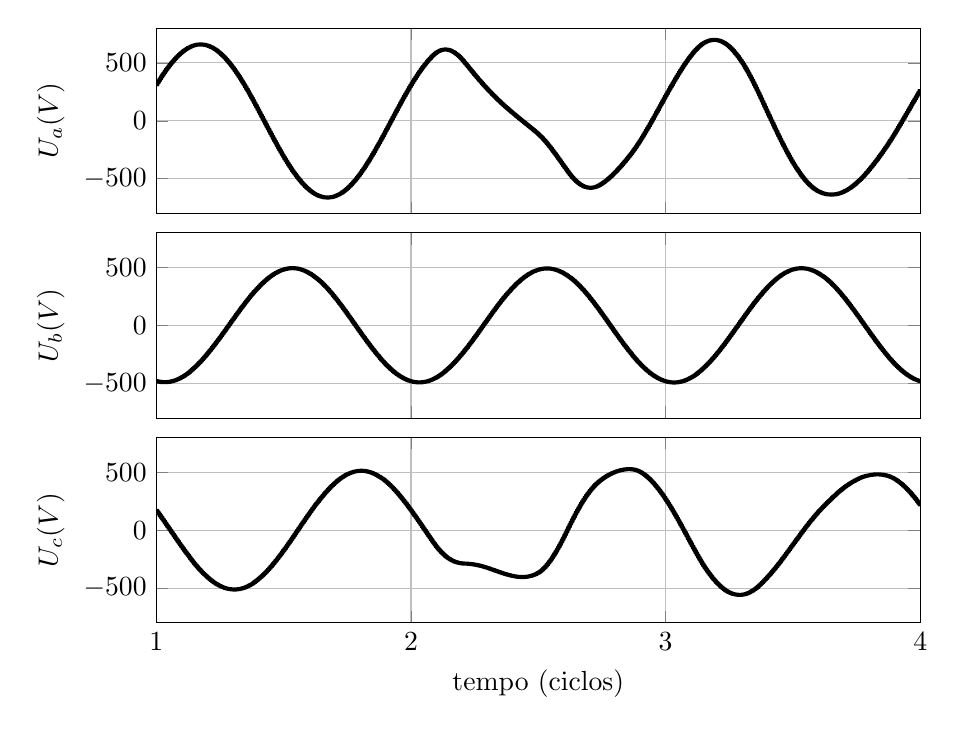
\begin{tikzpicture}

\begin{axis}[%
width=0.8\textwidth,
height=0.193917089240149\textwidth,
scale only axis,
xmin=0.0166666666666667,
xmax=0.0666666666666667,
xtick={0.0166666666666667,0.0333333333333333,0.05,0.0666666666666667},
xticklabels={\empty},
xmajorgrids,
ymin=-800,
ymax=800,
ytick={-500,    0,  500},
ylabel={$\text{U}_\text{b}\text{ (V)}$},
ymajorgrids,
name=plot2,
scaled x ticks = false,
legend columns=-1,
legend style={/tikz/every even column/.append style={column sep=0.3cm}},
legend style={font=\footnotesize}
]
\addplot [color=black,solid,line width=1.5pt,forget plot]
  table[row sep=crcr]{0.0166583333333333	-478.328989103039\\
0.0167	-481.372762295986\\
0.0167416666666667	-481.372762295986\\
0.0167833333333333	-483.944387417357\\
0.016825	-483.944387417357\\
0.0168666666666667	-486.043904769891\\
0.0169083333333333	-486.043904769891\\
0.01695	-487.669342075457\\
0.0169916666666667	-487.669342075457\\
0.0170333333333333	-488.81912329053\\
0.017075	-488.81912329053\\
0.0171166666666667	-489.492376222951\\
0.0171583333333333	-489.492376222951\\
0.0172	-489.689089295181\\
0.0172416666666667	-489.689089295181\\
0.0172833333333333	-489.410057478733\\
0.017325	-489.410057478733\\
0.0173666666666667	-488.656714544629\\
0.0174083333333333	-488.656714544629\\
0.01745	-487.430933830334\\
0.0174916666666667	-487.430933830334\\
0.0175333333333333	-485.734862735459\\
0.017575	-485.734862735459\\
0.0176166666666667	-483.570824107468\\
0.0176583333333333	-483.570824107468\\
0.0177	-480.941176730971\\
0.0177416666666667	-480.941176730971\\
0.0177833333333333	-477.848873406491\\
0.017825	-477.848873406491\\
0.0178666666666667	-474.296687037085\\
0.0179083333333333	-474.296687037085\\
0.01795	-470.287554266504\\
0.0179916666666667	-470.287554266504\\
0.0180333333333333	-465.824994538518\\
0.018075	-465.824994538518\\
0.0181166666666667	-460.912896166831\\
0.0181583333333333	-460.912896166831\\
0.0182	-455.555544349316\\
0.0182416666666667	-455.555544349316\\
0.0182833333333333	-449.757632700212\\
0.018325	-449.757632700212\\
0.0183666666666667	-443.524266807923\\
0.0184083333333333	-443.524266807923\\
0.01845	-436.860963041735\\
0.0184916666666667	-436.860963041735\\
0.0185333333333333	-429.773645406549\\
0.018575	-429.773645406549\\
0.0186166666666667	-422.2686421737\\
0.0186583333333333	-422.2686421737\\
0.0187	-414.352682994809\\
0.0187416666666667	-414.352682994809\\
0.0187833333333333	-406.710604021129\\
0.018825	-406.710604021129\\
0.0188666666666667	-396.968651829484\\
0.0189083333333333	-396.968651829484\\
0.01895	-387.24430030011\\
0.0189916666666667	-387.24430030011\\
0.0190333333333333	-377.413842111121\\
0.019075	-377.413842111121\\
0.0191166666666667	-367.3960735467\\
0.0191583333333333	-367.3960735467\\
0.0192	-357.12553953726\\
0.0192416666666667	-357.12553953726\\
0.0192833333333333	-346.559303382721\\
0.019325	-346.559303382721\\
0.0193666666666667	-335.674936708767\\
0.0194083333333333	-335.674936708767\\
0.01945	-324.465686057335\\
0.0194916666666667	-324.465686057335\\
0.0195333333333333	-312.935239244225\\
0.019575	-312.935239244225\\
0.0196166666666667	-301.093266862382\\
0.0196583333333333	-301.093266862382\\
0.0197	-288.95219973374\\
0.0197416666666667	-288.95219973374\\
0.0197833333333333	-276.525463982029\\
0.019825	-276.525463982029\\
0.0198666666666667	-263.82538033546\\
0.0199083333333333	-263.82538033546\\
0.01995	-250.865057706918\\
0.0199916666666667	-250.865057706918\\
0.0200333333333333	-237.656697428642\\
0.020075	-237.656697428642\\
0.0201166666666667	-224.212271375033\\
0.0201583333333333	-224.212271375033\\
0.0202	-210.543848998092\\
0.0202416666666667	-210.543848998092\\
0.0202833333333333	-196.6637735981\\
0.020325	-196.6637735981\\
0.0203666666666667	-182.584756063204\\
0.0204083333333333	-182.584756063204\\
0.02045	-168.319897946886\\
0.0204916666666667	-168.319897946886\\
0.0205333333333333	-153.882668002172\\
0.020575	-153.882668002172\\
0.0206166666666667	-139.286855686717\\
0.0206583333333333	-139.286855686717\\
0.0207	-124.546519243168\\
0.0207416666666667	-124.546519243168\\
0.0207833333333333	-109.675923407492\\
0.020825	-109.675923407492\\
0.0208666666666667	-94.6884951690301\\
0.0209083333333333	-94.6884951690301\\
0.02095	-79.6023211852309\\
0.0209916666666667	-79.6023211852309\\
0.0210333333333333	-64.4296541414652\\
0.021075	-64.4296541414652\\
0.0211166666666667	-49.1854677870168\\
0.0211583333333333	-49.1854677870168\\
0.0212	-33.8847697005379\\
0.0212416666666667	-33.8847697005379\\
0.0212833333333333	-18.5423320716325\\
0.021325	-18.5423320716325\\
0.0213666666666667	-3.1725945533516\\
0.0214083333333333	-3.1725945533516\\
0.02145	12.2102617721841\\
0.0214916666666667	12.2102617721841\\
0.0215333333333333	27.5921432856442\\
0.021575	27.5921432856442\\
0.0216166666666667	42.9588704890498\\
0.0216583333333333	42.9588704890498\\
0.0217	58.2960537853681\\
0.0217416666666667	58.2960537853681\\
0.0217833333333333	73.5890384864759\\
0.021825	73.5890384864759\\
0.0218666666666667	88.82269659409\\
0.0219083333333333	88.82269659409\\
0.02195	103.982669291038\\
0.0219916666666667	103.982669291038\\
0.0220333333333333	119.053037141893\\
0.022075	119.053037141893\\
0.0221166666666667	134.01853586672\\
0.0221583333333333	134.01853586672\\
0.0222	148.863909368128\\
0.0222416666666667	148.863909368128\\
0.0222833333333333	163.573956427556\\
0.022325	163.573956427556\\
0.0223666666666667	178.133568427636\\
0.0224083333333333	178.133568427636\\
0.02245	192.527757716713\\
0.0224916666666667	192.527757716713\\
0.0225333333333333	206.741679404245\\
0.022575	206.741679404245\\
0.0226166666666667	220.760649670751\\
0.0226583333333333	220.760649670751\\
0.0227	234.570162946369\\
0.0227416666666667	234.570162946369\\
0.0227833333333333	248.155909263895\\
0.022825	248.155909263895\\
0.0228666666666667	261.687830320942\\
0.0229083333333333	261.687830320942\\
0.02295	274.986604079196\\
0.0229916666666667	274.986604079196\\
0.0230333333333333	286.928801747272\\
0.023075	286.928801747272\\
0.0231166666666667	298.950506950644\\
0.0231583333333333	298.950506950644\\
0.0232	310.924864102034\\
0.0232416666666667	310.924864102034\\
0.0232833333333333	322.756989832147\\
0.023325	322.756989832147\\
0.0233666666666667	334.367084014297\\
0.0234083333333333	334.367084014297\\
0.02345	345.69602196514\\
0.0234916666666667	345.69602196514\\
0.0235333333333333	356.703461032175\\
0.023575	356.703461032175\\
0.0236166666666667	367.363371170442\\
0.0236583333333333	367.363371170442\\
0.0237	377.659204280424\\
0.0237416666666667	377.659204280424\\
0.0237833333333333	387.579795487262\\
0.023825	387.579795487262\\
0.0238666666666667	397.116425283701\\
0.0239083333333333	397.116425283701\\
0.02395	406.261310362139\\
0.0239916666666667	406.261310362139\\
0.0240333333333333	415.0053223807\\
0.024075	415.0053223807\\
0.0241166666666667	423.340732147141\\
0.0241583333333333	423.340732147141\\
0.0242	431.258683016742\\
0.0242416666666667	431.258683016742\\
0.0242833333333333	438.750365395371\\
0.024325	438.750365395371\\
0.0243666666666667	445.807262831054\\
0.0244083333333333	445.807262831054\\
0.02445	452.421342397773\\
0.0244916666666667	452.421342397773\\
0.0245333333333333	458.585161293933\\
0.024575	458.585161293933\\
0.0246166666666667	464.291905294308\\
0.0246583333333333	464.291905294308\\
0.0247	469.535383109734\\
0.0247416666666667	469.535383109734\\
0.0247833333333333	474.309999446141\\
0.024825	474.309999446141\\
0.0248666666666667	478.610723480444\\
0.0249083333333333	478.610723480444\\
0.02495	482.432523836755\\
0.0249916666666667	482.432523836755\\
0.0250333333333333	485.772612186125\\
0.025075	485.772612186125\\
0.0251166666666667	488.627883686145\\
0.0251583333333333	488.627883686145\\
0.0252	490.994391489966\\
0.0252416666666667	490.994391489966\\
0.0252833333333333	492.869784189106\\
0.025325	492.869784189106\\
0.0253666666666667	494.252063559781\\
0.0254083333333333	494.252063559781\\
0.02545	495.139387583695\\
0.0254916666666667	495.139387583695\\
0.0255333333333333	495.530061759552\\
0.025575	495.530061759552\\
0.0256166666666667	495.422663936061\\
0.0256583333333333	495.422663936061\\
0.0257	494.816230581684\\
0.0257416666666667	494.816230581684\\
0.0257833333333333	493.710425995119\\
0.025825	493.710425995119\\
0.0258666666666667	492.105654148384\\
0.0259083333333333	492.105654148384\\
0.02595	490.003108134894\\
0.0259916666666667	490.003108134894\\
0.0260333333333333	487.404961487327\\
0.026075	487.404961487327\\
0.0261166666666667	484.313069214194\\
0.0261583333333333	484.313069214194\\
0.0262	480.731558886196\\
0.0262416666666667	480.731558886196\\
0.0262833333333333	476.664323712434\\
0.026325	476.664323712434\\
0.0263666666666667	472.115829454631\\
0.0264083333333333	472.115829454631\\
0.02645	467.091068733291\\
0.0264916666666667	467.091068733291\\
0.0265333333333333	461.595540479995\\
0.026575	461.595540479995\\
0.0266166666666667	455.635234907076\\
0.0266583333333333	455.635234907076\\
0.0267	449.21662231492\\
0.0267416666666667	449.21662231492\\
0.0267833333333333	442.346643428456\\
0.026825	442.346643428456\\
0.0268666666666667	435.032699614098\\
0.0269083333333333	435.032699614098\\
0.02695	427.282642172915\\
0.0269916666666667	427.282642172915\\
0.0270333333333333	418.527982244731\\
0.027075	418.527982244731\\
0.0271166666666667	410.672570182659\\
0.0271583333333333	410.672570182659\\
0.0272	402.276872290978\\
0.0272416666666667	402.276872290978\\
0.0272833333333333	393.223850223727\\
0.027325	393.223850223727\\
0.0273666666666667	383.609151155178\\
0.0274083333333333	383.609151155178\\
0.02745	373.508718653929\\
0.0274916666666667	373.508718653929\\
0.0275333333333333	362.979579538073\\
0.027575	362.979579538073\\
0.0276166666666667	352.061894709897\\
0.0276583333333333	352.061894709897\\
0.0277	340.783205444461\\
0.0277416666666667	340.783205444461\\
0.0277833333333333	329.162781541968\\
0.027825	329.162781541968\\
0.0278666666666667	317.215226351439\\
0.0279083333333333	317.215226351439\\
0.02795	304.953068995059\\
0.0279916666666667	304.953068995059\\
0.0280333333333333	292.388308765939\\
0.028075	292.388308765939\\
0.0281166666666667	279.533394256386\\
0.0281583333333333	279.533394256386\\
0.0282	266.401997020689\\
0.0282416666666667	266.401997020689\\
0.0282833333333333	253.007121767018\\
0.028325	253.007121767018\\
0.0283666666666667	239.363037342399\\
0.0284083333333333	239.363037342399\\
0.02845	225.484309796947\\
0.0284916666666667	225.484309796947\\
0.0285333333333333	211.385672071801\\
0.028575	211.385672071801\\
0.0286166666666667	197.081935254737\\
0.0286583333333333	197.081935254737\\
0.0287	182.587950486431\\
0.0287416666666667	182.587950486431\\
0.0287833333333333	167.918604082923\\
0.028825	167.918604082923\\
0.0288666666666667	153.088829011011\\
0.0289083333333333	153.088829011011\\
0.02895	138.113619934855\\
0.0289916666666667	138.113619934855\\
0.0290333333333333	123.008044204917\\
0.029075	123.008044204917\\
0.0291166666666667	107.788100944899\\
0.0291583333333333	107.788100944899\\
0.0292	92.4664220892656\\
0.0292416666666667	92.4664220892656\\
0.0292833333333333	77.0599110293703\\
0.029325	77.0599110293703\\
0.0293666666666667	61.5839402726698\\
0.0294083333333333	61.5839402726698\\
0.02945	46.0538191073489\\
0.0294916666666667	46.0538191073489\\
0.0295333333333333	30.4851141949034\\
0.029575	30.4851141949034\\
0.0296166666666667	14.8937682112207\\
0.0296583333333333	14.8937682112207\\
0.0297	-0.703957306529608\\
0.0297416666666667	-0.703957306529608\\
0.0297833333333333	-16.2916492298269\\
0.029825	-16.2916492298269\\
0.0298666666666667	-31.8529362123827\\
0.0299083333333333	-31.8529362123827\\
0.02995	-47.371649369948\\
0.0299916666666667	-47.371649369948\\
0.0300333333333333	-62.8319222299047\\
0.030075	-62.8319222299047\\
0.0301166666666667	-78.2183969102601\\
0.0301583333333333	-78.2183969102601\\
0.0302	-93.5154108314719\\
0.0302416666666667	-93.5154108314719\\
0.0302833333333333	-108.70816278091\\
0.030325	-108.70816278091\\
0.0303666666666667	-123.782356080195\\
0.0304083333333333	-123.782356080195\\
0.03045	-138.723507249364\\
0.0304916666666667	-138.723507249364\\
0.0305333333333333	-153.517339096442\\
0.030575	-153.517339096442\\
0.0306166666666667	-168.149764544084\\
0.0306583333333333	-168.149764544084\\
0.0307	-182.60688669631\\
0.0307416666666667	-182.60688669631\\
0.0307833333333333	-196.875004412733\\
0.030825	-196.875004412733\\
0.0308666666666667	-210.940621254231\\
0.0309083333333333	-210.940621254231\\
0.03095	-224.790455634942\\
0.0309916666666667	-224.790455634942\\
0.0310333333333333	-238.411450801645\\
0.031075	-238.411450801645\\
0.0311166666666667	-251.788204920739\\
0.0311583333333333	-251.788204920739\\
0.0312	-264.319493294975\\
0.0312416666666667	-264.319493294975\\
0.0312833333333333	-278.081845363642\\
0.031325	-278.081845363642\\
0.0313666666666667	-291.211888263673\\
0.0314083333333333	-291.211888263673\\
0.03145	-303.807007713181\\
0.0314916666666667	-303.807007713181\\
0.0315333333333333	-315.936364357588\\
0.031575	-315.936364357588\\
0.0316166666666667	-327.655020751537\\
0.0316583333333333	-327.655020751537\\
0.0317	-338.998550237152\\
0.0317416666666667	-338.998550237152\\
0.0317833333333333	-349.984949605885\\
0.031825	-349.984949605885\\
0.0318666666666667	-360.618974262017\\
0.0319083333333333	-360.618974262017\\
0.03195	-370.896795074955\\
0.0319916666666667	-370.896795074955\\
0.0320333333333333	-380.809923421548\\
0.032075	-380.809923421548\\
0.0321166666666667	-390.348041070204\\
0.0321583333333333	-390.348041070204\\
0.0322	-399.500455565927\\
0.0322416666666667	-399.500455565927\\
0.0322833333333333	-408.258433783543\\
0.032325	-408.258433783543\\
0.0323666666666667	-416.612673979994\\
0.0324083333333333	-416.612673979994\\
0.03245	-424.555376388038\\
0.0324916666666667	-424.555376388038\\
0.0325333333333333	-432.079651399668\\
0.032575	-432.079651399668\\
0.0326166666666667	-439.17912856472\\
0.0326583333333333	-439.17912856472\\
0.0327	-445.847803165625\\
0.0327416666666667	-445.847803165625\\
0.0327833333333333	-452.079952433882\\
0.032825	-452.079952433882\\
0.0328666666666667	-457.870112681898\\
0.0329083333333333	-457.870112681898\\
0.03295	-463.213095942823\\
0.0329916666666667	-463.213095942823\\
0.0330333333333333	-468.104025539882\\
0.033075	-468.104025539882\\
0.0331166666666667	-472.538375275198\\
0.0331583333333333	-472.538375275198\\
0.0332	-476.512043591712\\
0.0332416666666667	-476.512043591712\\
0.0332833333333333	-480.021998518076\\
0.033325	-480.021998518076\\
0.0333666666666667	-483.062409528906\\
0.0334083333333333	-483.062409528906\\
0.03345	-485.632179354782\\
0.0334916666666667	-485.632179354782\\
0.0335333333333333	-487.728811385411\\
0.033575	-487.728811385411\\
0.0336166666666667	-489.350303992202\\
0.0336583333333333	-489.350303992202\\
0.0337	-490.495382636273\\
0.0337416666666667	-490.495382636273\\
0.0337833333333333	-491.163571670944\\
0.033825	-491.163571670944\\
0.0338666666666667	-491.355115539431\\
0.0339083333333333	-491.355115539431\\
0.03395	-491.070817444326\\
0.0339916666666667	-491.070817444326\\
0.0340333333333333	-490.311872482351\\
0.034075	-490.311872482351\\
0.0341166666666667	-489.079743497884\\
0.0341583333333333	-489.079743497884\\
0.0342	-487.376098124238\\
0.0342416666666667	-487.376098124238\\
0.0342833333333333	-485.20249992764\\
0.034325	-485.20249992764\\
0.0343666666666667	-482.562089146938\\
0.0344083333333333	-482.562089146938\\
0.03445	-479.456339884062\\
0.0344916666666667	-479.456339884062\\
0.0345333333333333	-475.887666587193\\
0.034575	-475.887666587193\\
0.0346166666666667	-471.862477669189\\
0.0346583333333333	-471.862477669189\\
0.0347	-467.386376616343\\
0.0347416666666667	-467.386376616343\\
0.0347833333333333	-462.460204193963\\
0.034825	-462.460204193963\\
0.0348666666666667	-457.084993467022\\
0.0349083333333333	-457.084993467022\\
0.03495	-451.264285123146\\
0.0349916666666667	-451.264285123146\\
0.0350333333333333	-445.003485871476\\
0.035075	-445.003485871476\\
0.0351166666666667	-438.309126556655\\
0.0351583333333333	-438.309126556655\\
0.0352	-431.188237094164\\
0.0352416666666667	-431.188237094164\\
0.0352833333333333	-423.843217345319\\
0.035325	-423.843217345319\\
0.0353666666666667	-416.006961069986\\
0.0354083333333333	-416.006961069986\\
0.03545	-406.872705407128\\
0.0354916666666667	-406.872705407128\\
0.0355333333333333	-397.652348142447\\
0.035575	-397.652348142447\\
0.0356166666666667	-388.257619044804\\
0.0356583333333333	-388.257619044804\\
0.0357	-378.623360239847\\
0.0357416666666667	-378.623360239847\\
0.0357833333333333	-368.698593317024\\
0.035825	-368.698593317024\\
0.0358666666666667	-358.451057487075\\
0.0359083333333333	-358.451057487075\\
0.03595	-347.865419222676\\
0.0359916666666667	-347.865419222676\\
0.0360333333333333	-336.939196124305\\
0.036075	-336.939196124305\\
0.0361166666666667	-325.678369718751\\
0.0361583333333333	-325.678369718751\\
0.0362	-314.093684159792\\
0.0362416666666667	-314.093684159792\\
0.0362833333333333	-302.19760657953\\
0.036325	-302.19760657953\\
0.0363666666666667	-290.003073678589\\
0.0364083333333333	-290.003073678589\\
0.03645	-277.521539253932\\
0.0364916666666667	-277.521539253932\\
0.0365333333333333	-264.76677178694\\
0.036575	-264.76677178694\\
0.0366166666666667	-251.75138810459\\
0.0366583333333333	-251.75138810459\\
0.0367	-238.484219164876\\
0.0367416666666667	-238.484219164876\\
0.0367833333333333	-224.974868835818\\
0.036825	-224.974868835818\\
0.0368666666666667	-211.237477773964\\
0.0369083333333333	-211.237477773964\\
0.03695	-197.287072811055\\
0.0369916666666667	-197.287072811055\\
0.0370333333333333	-183.137914989065\\
0.037075	-183.137914989065\\
0.0371166666666667	-168.803978576591\\
0.0371583333333333	-168.803978576591\\
0.0372	-154.298661037236\\
0.0372416666666667	-154.298661037236\\
0.0372833333333333	-139.634992651273\\
0.037325	-139.634992651273\\
0.0373666666666667	-124.826036658058\\
0.0374083333333333	-124.826036658058\\
0.03745	-109.886448376808\\
0.0374916666666667	-109.886448376808\\
0.0375333333333333	-94.8311105238512\\
0.037575	-94.8311105238512\\
0.0376166666666667	-79.6741457005464\\
0.0376583333333333	-79.6741457005464\\
0.0377	-64.430915589704\\
0.0377416666666667	-64.430915589704\\
0.0377833333333333	-49.1168958380644\\
0.037825	-49.1168958380644\\
0.0378666666666667	-33.7474109692533\\
0.0379083333333333	-33.7474109692533\\
0.03795	-18.3375525391689\\
0.0379916666666667	-18.3375525391689\\
0.0380333333333333	-2.9021014951139\\
0.038075	-2.9021014951139\\
0.0381166666666667	12.5441649238791\\
0.0381583333333333	12.5441649238791\\
0.0382	27.9862135071296\\
0.0382416666666667	27.9862135071296\\
0.0382833333333333	43.4088160189249\\
0.038325	43.4088160189249\\
0.0383666666666667	58.7964709733482\\
0.0384083333333333	58.7964709733482\\
0.03845	74.1332705553863\\
0.0384916666666667	74.1332705553863\\
0.0385333333333333	89.4046588216954\\
0.038575	89.4046588216954\\
0.0386166666666667	104.5941845202\\
0.0386583333333333	104.5941845202\\
0.0387	119.686452596076\\
0.0387416666666667	119.686452596076\\
0.0387833333333333	134.66627355262\\
0.038825	134.66627355262\\
0.0388666666666667	149.518283336125\\
0.0389083333333333	149.518283336125\\
0.03895	164.226788249997\\
0.0389916666666667	164.226788249997\\
0.0390333333333333	178.776134246639\\
0.039075	178.776134246639\\
0.0391166666666667	193.150979209617\\
0.0391583333333333	193.150979209617\\
0.0392	207.336383906119\\
0.0392416666666667	207.336383906119\\
0.0392833333333333	221.317782891681\\
0.039325	221.317782891681\\
0.0393666666666667	235.080917713056\\
0.0394083333333333	235.080917713056\\
0.03945	249.106017709465\\
0.0394916666666667	249.106017709465\\
0.0395333333333333	261.782981387672\\
0.039575	261.782981387672\\
0.0396166666666667	274.244693954053\\
0.0396583333333333	274.244693954053\\
0.0397	286.670435385755\\
0.0397416666666667	286.670435385755\\
0.0397833333333333	298.9701138084\\
0.039825	298.9701138084\\
0.0398666666666667	311.070470544628\\
0.0399083333333333	311.070470544628\\
0.03995	322.915197067812\\
0.0399916666666667	322.915197067812\\
0.0400333333333333	334.464145520092\\
0.040075	334.464145520092\\
0.0401166666666667	345.689797905232\\
0.0401583333333333	345.689797905232\\
0.0402	356.573569549156\\
0.0402416666666667	356.573569549156\\
0.0402833333333333	367.102419833383\\
0.040325	367.102419833383\\
0.0403666666666667	377.266336550431\\
0.0404083333333333	377.266336550431\\
0.04045	387.056723613013\\
0.0404916666666667	387.056723613013\\
0.0405333333333333	396.465185002339\\
0.040575	396.465185002339\\
0.0406166666666667	405.482553450114\\
0.0406583333333333	405.482553450114\\
0.0407	414.100873536397\\
0.0407416666666667	414.100873536397\\
0.0407833333333333	422.311068387454\\
0.040825	422.311068387454\\
0.0408666666666667	430.103823202378\\
0.0409083333333333	430.103823202378\\
0.04095	437.470785539434\\
0.0409916666666667	437.470785539434\\
0.0410333333333333	444.404904032625\\
0.041075	444.404904032625\\
0.0411166666666667	450.899745696091\\
0.0411583333333333	450.899745696091\\
0.0412	456.949290210676\\
0.0412416666666667	456.949290210676\\
0.0412833333333333	462.548172385588\\
0.041325	462.548172385588\\
0.0413666666666667	467.690509791918\\
0.0414083333333333	467.690509791918\\
0.04145	472.368093229522\\
0.0414916666666667	472.368093229522\\
0.0415333333333333	476.574672015731\\
0.041575	476.574672015731\\
0.0416166666666667	480.310156693439\\
0.0416583333333333	480.310156693439\\
0.0417	483.572332768667\\
0.0417416666666667	483.572332768667\\
0.0417833333333333	486.359289598516\\
0.041825	486.359289598516\\
0.0418666666666667	488.668565715516\\
0.0419083333333333	488.668565715516\\
0.04195	490.497331626202\\
0.0419916666666667	490.497331626202\\
0.0420333333333333	491.842670843953\\
0.042075	491.842670843953\\
0.0421166666666667	492.699071140014\\
0.0421583333333333	492.699071140014\\
0.0422	493.068619758159\\
0.0422416666666667	493.068619758159\\
0.0422833333333333	492.952466583921\\
0.042325	492.952466583921\\
0.0423666666666667	492.347367558496\\
0.0424083333333333	492.347367558496\\
0.04245	491.252031478426\\
0.0424916666666667	491.252031478426\\
0.0425333333333333	489.667385633026\\
0.042575	489.667385633026\\
0.0426166666666667	487.594910620982\\
0.0426583333333333	487.594910620982\\
0.0427	485.037655582358\\
0.0427416666666667	485.037655582358\\
0.0427833333333333	481.999497712266\\
0.042825	481.999497712266\\
0.0428666666666667	478.483785993532\\
0.0429083333333333	478.483785993532\\
0.04295	474.494421900634\\
0.0429916666666667	474.494421900634\\
0.0430333333333333	470.035506802172\\
0.043075	470.035506802172\\
0.0431166666666667	465.111295250602\\
0.0431583333333333	465.111295250602\\
0.0432	459.726505545849\\
0.0432416666666667	459.726505545849\\
0.0432833333333333	453.886192967286\\
0.043325	453.886192967286\\
0.0433666666666667	447.595582698072\\
0.0434083333333333	447.595582698072\\
0.04345	440.861630320738\\
0.0434916666666667	440.861630320738\\
0.0435333333333333	433.681731049463\\
0.043575	433.681731049463\\
0.0436166666666667	425.580511912541\\
0.0436583333333333	425.580511912541\\
0.0437	418.359521795389\\
0.0437416666666667	418.359521795389\\
0.0437833333333333	410.424839442397\\
0.043825	410.424839442397\\
0.0438666666666667	401.856433443567\\
0.0439083333333333	401.856433443567\\
0.04395	392.738907245265\\
0.0439916666666667	392.738907245265\\
0.0440333333333333	383.143262572768\\
0.044075	383.143262572768\\
0.0441166666666667	373.122289947879\\
0.0441583333333333	373.122289947879\\
0.0442	362.712148769228\\
0.0442416666666667	362.712148769228\\
0.0442833333333333	351.936466122906\\
0.044325	351.936466122906\\
0.0443666666666667	340.81070596891\\
0.0444083333333333	340.81070596891\\
0.04445	329.346076655623\\
0.0444916666666667	329.346076655623\\
0.0445333333333333	317.552138040485\\
0.044575	317.552138040485\\
0.0446166666666667	305.438801181686\\
0.0446583333333333	305.438801181686\\
0.0447	293.018741534484\\
0.0447416666666667	293.018741534484\\
0.0447833333333333	280.303286512468\\
0.044825	280.303286512468\\
0.0448666666666667	267.304839178201\\
0.0449083333333333	267.304839178201\\
0.04495	254.036587804692\\
0.0449916666666667	254.036587804692\\
0.0450333333333333	240.512194679208\\
0.045075	240.512194679208\\
0.0451166666666667	226.745693466081\\
0.0451583333333333	226.745693466081\\
0.0452	212.751335137093\\
0.0452416666666667	212.751335137093\\
0.0452833333333333	198.543785808771\\
0.045325	198.543785808771\\
0.0453666666666667	184.137961271205\\
0.0454083333333333	184.137961271205\\
0.04545	169.549083751309\\
0.0454916666666667	169.549083751309\\
0.0455333333333333	154.791278668457\\
0.045575	154.791278668457\\
0.0456166666666667	139.877896565075\\
0.0456583333333333	139.877896565075\\
0.0457	124.824761922009\\
0.0457416666666667	124.824761922009\\
0.0457833333333333	109.646732276147\\
0.045825	109.646732276147\\
0.0458666666666667	94.3613000585707\\
0.0459083333333333	94.3613000585707\\
0.04595	78.9840886019565\\
0.0459916666666667	78.9840886019565\\
0.0460333333333333	63.5303702887837\\
0.046075	63.5303702887837\\
0.0461166666666667	48.0155535189244\\
0.0461583333333333	48.0155535189244\\
0.0462	32.4561326759275\\
0.0462416666666667	32.4561326759275\\
0.0462833333333333	16.8700891761257\\
0.046325	16.8700891761257\\
0.0463666666666667	1.26865974731029\\
0.0464083333333333	1.26865974731029\\
0.04645	-14.3325199650595\\
0.0464916666666667	-14.3325199650595\\
0.0465333333333333	-29.9131132460085\\
0.046575	-29.9131132460085\\
0.0466166666666667	-45.4562368559247\\
0.0466583333333333	-45.4562368559247\\
0.0467	-60.9463194667191\\
0.0467416666666667	-60.9463194667191\\
0.0467833333333333	-76.3667309691358\\
0.046825	-76.3667309691358\\
0.0468666666666667	-91.7034974678986\\
0.0469083333333333	-91.7034974678986\\
0.04695	-106.941680966748\\
0.0469916666666667	-106.941680966748\\
0.0470333333333333	-122.066146305108\\
0.047075	-122.066146305108\\
0.0471166666666667	-137.06188382755\\
0.0471583333333333	-137.06188382755\\
0.0472	-151.913815267241\\
0.0472416666666667	-151.913815267241\\
0.0472833333333333	-166.607053394949\\
0.047325	-166.607053394949\\
0.0473666666666667	-181.127077064277\\
0.0474083333333333	-181.127077064277\\
0.04745	-195.459743543001\\
0.0474916666666667	-195.459743543001\\
0.0475333333333333	-209.591362819321\\
0.047575	-209.591362819321\\
0.0476166666666667	-223.506823346012\\
0.0476583333333333	-223.506823346012\\
0.0477	-237.00101652442\\
0.0477416666666667	-237.00101652442\\
0.0477833333333333	-250.375370605446\\
0.047825	-250.375370605446\\
0.0478666666666667	-264.247228944917\\
0.0479083333333333	-264.247228944917\\
0.04795	-277.57583918717\\
0.0479916666666667	-277.57583918717\\
0.0480333333333333	-290.432998246762\\
0.048075	-290.432998246762\\
0.0481166666666667	-302.874898420103\\
0.0481583333333333	-302.874898420103\\
0.0482	-314.943125188458\\
0.0482416666666667	-314.943125188458\\
0.0482833333333333	-326.662290446261\\
0.048325	-326.662290446261\\
0.0483666666666667	-338.042278959217\\
0.0484083333333333	-338.042278959217\\
0.04845	-349.082657598953\\
0.0484916666666667	-349.082657598953\\
0.0485333333333333	-359.776933252618\\
0.048575	-359.776933252618\\
0.0486166666666667	-370.115682517757\\
0.0486583333333333	-370.115682517757\\
0.0487	-380.088397551359\\
0.0487416666666667	-380.088397551359\\
0.0487833333333333	-389.684585375337\\
0.048825	-389.684585375337\\
0.0488666666666667	-398.896409543848\\
0.0489083333333333	-398.896409543848\\
0.04895	-407.713702687894\\
0.0489916666666667	-407.713702687894\\
0.0490333333333333	-416.128294513139\\
0.049075	-416.128294513139\\
0.0491166666666667	-424.133317051478\\
0.0491583333333333	-424.133317051478\\
0.0492	-431.722331990266\\
0.0492416666666667	-431.722331990266\\
0.0492833333333333	-438.889026645031\\
0.049325	-438.889026645031\\
0.0493666666666667	-445.627341957187\\
0.0494083333333333	-445.627341957187\\
0.04945	-451.931076637639\\
0.0494916666666667	-451.931076637639\\
0.0495333333333333	-457.794069196784\\
0.049575	-457.794069196784\\
0.0496166666666667	-463.210591616737\\
0.0496583333333333	-463.210591616737\\
0.0497	-468.174796015772\\
0.0497416666666667	-468.174796015772\\
0.0497833333333333	-472.68195994869\\
0.049825	-472.68195994869\\
0.0498666666666667	-476.727789100183\\
0.0499083333333333	-476.727789100183\\
0.04995	-480.308346767437\\
0.0499916666666667	-480.308346767437\\
0.0500333333333333	-483.420977339502\\
0.050075	-483.420977339502\\
0.0501166666666667	-486.062497335619\\
0.0501583333333333	-486.062497335619\\
0.0502	-488.230133182561\\
0.0502416666666667	-488.230133182561\\
0.0502833333333333	-489.921561624727\\
0.050325	-489.921561624727\\
0.0503666666666667	-491.136204240014\\
0.0504083333333333	-491.136204240014\\
0.05045	-491.872508123106\\
0.0504916666666667	-491.872508123106\\
0.0505333333333333	-492.129861840952\\
0.050575	-492.129861840952\\
0.0506166666666667	-491.909659809047\\
0.0506583333333333	-491.909659809047\\
0.0507	-491.213010719094\\
0.0507416666666667	-491.213010719094\\
0.0507833333333333	-490.040835198961\\
0.050825	-490.040835198961\\
0.0508666666666667	-488.394120133251\\
0.0509083333333333	-488.394120133251\\
0.05095	-486.275366201401\\
0.0509916666666667	-486.275366201401\\
0.0510333333333333	-483.685389331488\\
0.051075	-483.685389331488\\
0.0511166666666667	-480.626415285703\\
0.0511583333333333	-480.626415285703\\
0.0512	-477.100789926303\\
0.0512416666666667	-477.100789926303\\
0.0512833333333333	-473.111388437613\\
0.051325	-473.111388437613\\
0.0513666666666667	-468.661612023946\\
0.0514083333333333	-468.661612023946\\
0.05145	-463.755404955367\\
0.0514916666666667	-463.755404955367\\
0.0515333333333333	-458.397218599947\\
0.051575	-458.397218599947\\
0.0516166666666667	-452.591883879653\\
0.0516583333333333	-452.591883879653\\
0.0517	-446.344659833732\\
0.0517416666666667	-446.344659833732\\
0.0517833333333333	-439.661834530548\\
0.051825	-439.661834530548\\
0.0518666666666667	-432.973201373906\\
0.0519083333333333	-432.973201373906\\
0.05195	-424.9238177607\\
0.0519916666666667	-424.9238177607\\
0.0520333333333333	-416.454872243868\\
0.052075	-416.454872243868\\
0.0521166666666667	-407.796123452613\\
0.0521583333333333	-407.796123452613\\
0.0522	-398.881834393278\\
0.0522416666666667	-398.881834393278\\
0.0522833333333333	-389.663103951547\\
0.052325	-389.663103951547\\
0.0523666666666667	-380.109879074884\\
0.0524083333333333	-380.109879074884\\
0.05245	-370.205171386402\\
0.0524916666666667	-370.205171386402\\
0.0525333333333333	-359.94008009255\\
0.052575	-359.94008009255\\
0.0526166666666667	-349.317994044045\\
0.0526583333333333	-349.317994044045\\
0.0527	-338.350133889017\\
0.0527416666666667	-338.350133889017\\
0.0527833333333333	-327.048470451454\\
0.052825	-327.048470451454\\
0.0528666666666667	-315.424680843599\\
0.0529083333333333	-315.424680843599\\
0.05295	-303.48972268604\\
0.0529916666666667	-303.48972268604\\
0.0530333333333333	-291.253697717625\\
0.053075	-291.253697717625\\
0.0531166666666667	-278.729847006983\\
0.0531583333333333	-278.729847006983\\
0.0532	-265.929627652681\\
0.0532416666666667	-265.929627652681\\
0.0532833333333333	-252.864003527286\\
0.053325	-252.864003527286\\
0.0533666666666667	-239.545390879813\\
0.0534083333333333	-239.545390879813\\
0.05345	-225.986736413012\\
0.0534916666666667	-225.986736413012\\
0.0535333333333333	-212.200997373425\\
0.053575	-212.200997373425\\
0.0536166666666667	-198.20178050543\\
0.0536583333333333	-198.20178050543\\
0.0537	-184.002976664328\\
0.0537416666666667	-184.002976664328\\
0.0537833333333333	-169.618777516532\\
0.053825	-169.618777516532\\
0.0538666666666667	-155.063258633972\\
0.0539083333333333	-155.063258633972\\
0.05395	-140.350010974899\\
0.0539916666666667	-140.350010974899\\
0.0540333333333333	-125.494490383426\\
0.054075	-125.494490383426\\
0.0541166666666667	-110.510483878359\\
0.0541583333333333	-110.510483878359\\
0.0542	-95.41256883096\\
0.0542416666666667	-95.41256883096\\
0.0542833333333333	-80.2157610667614\\
0.054325	-80.2157610667614\\
0.0543666666666667	-64.9345150980876\\
0.0544083333333333	-64.9345150980876\\
0.05445	-49.582007143794\\
0.0544916666666667	-49.582007143794\\
0.0545333333333333	-34.1736602074678\\
0.054575	-34.1736602074678\\
0.0546166666666667	-18.7290780256136\\
0.0546583333333333	-18.7290780256136\\
0.0547	-3.26173930788178\\
0.0547416666666667	-3.26173930788178\\
0.0547833333333333	12.2173123034477\\
0.054825	12.2173123034477\\
0.0548666666666667	27.6939042936501\\
0.0549083333333333	27.6939042936501\\
0.05495	43.1527392039165\\
0.0549916666666667	43.1527392039165\\
0.0550333333333333	58.5788251481509\\
0.055075	58.5788251481509\\
0.0551166666666667	73.9562327104943\\
0.0551583333333333	73.9562327104943\\
0.0552	89.2687363785002\\
0.0552416666666667	89.2687363785002\\
0.0552833333333333	104.500594808725\\
0.055325	104.500594808725\\
0.0553666666666667	119.636116228614\\
0.0554083333333333	119.636116228614\\
0.05545	134.66002337835\\
0.0554916666666667	134.66002337835\\
0.0555333333333333	149.557265295072\\
0.055575	149.557265295072\\
0.0556166666666667	164.312975721939\\
0.0556583333333333	164.312975721939\\
0.0557	178.912414426348\\
0.0557416666666667	178.912414426348\\
0.0557833333333333	193.340869617833\\
0.055825	193.340869617833\\
0.0558666666666667	207.584047711812\\
0.0559083333333333	207.584047711812\\
0.05595	221.649592508348\\
0.0559916666666667	221.649592508348\\
0.0560333333333333	235.90179407268\\
0.056075	235.90179407268\\
0.0561166666666667	248.812050467668\\
0.0561583333333333	248.812050467668\\
0.0562	261.728072869779\\
0.0562416666666667	261.728072869779\\
0.0562833333333333	274.589043397849\\
0.056325	274.589043397849\\
0.0563666666666667	287.31251086188\\
0.0564083333333333	287.31251086188\\
0.05645	299.831678661534\\
0.0564916666666667	299.831678661534\\
0.0565333333333333	312.096762723358\\
0.056575	312.096762723358\\
0.0566166666666667	324.069560647856\\
0.0566583333333333	324.069560647856\\
0.0567	335.722240967018\\
0.0567416666666667	335.722240967018\\
0.0567833333333333	347.040245671561\\
0.056825	347.040245671561\\
0.0568666666666667	358.013968498111\\
0.0569083333333333	358.013968498111\\
0.05695	368.633291023524\\
0.0569916666666667	368.633291023524\\
0.0570333333333333	378.888273019104\\
0.057075	378.888273019104\\
0.0571166666666667	388.767403823566\\
0.0571583333333333	388.767403823566\\
0.0572	398.261089815887\\
0.0572416666666667	398.261089815887\\
0.0572833333333333	407.360397631016\\
0.057325	407.360397631016\\
0.0573666666666667	416.054641235888\\
0.0574083333333333	416.054641235888\\
0.05745	424.333358541391\\
0.0574916666666667	424.333358541391\\
0.0575333333333333	432.187892531853\\
0.057575	432.187892531853\\
0.0576166666666667	439.609718478329\\
0.0576583333333333	439.609718478329\\
0.0577	446.59114928807\\
0.0577416666666667	446.59114928807\\
0.0577833333333333	453.125291550232\\
0.057825	453.125291550232\\
0.0578666666666667	459.205492698452\\
0.0579083333333333	459.205492698452\\
0.05795	464.826013093453\\
0.0579916666666667	464.826013093453\\
0.0580333333333333	469.980808563756\\
0.058075	469.980808563756\\
0.0581166666666667	474.663968749913\\
0.0581583333333333	474.663968749913\\
0.0582	478.872042176142\\
0.0582416666666667	478.872042176142\\
0.0582833333333333	482.600041203607\\
0.058325	482.600041203607\\
0.0583666666666667	485.844448523412\\
0.0584083333333333	485.844448523412\\
0.05845	488.602523024656\\
0.0584916666666667	488.602523024656\\
0.0585333333333333	490.870411501712\\
0.058575	490.870411501712\\
0.0586166666666667	492.645347334968\\
0.0586583333333333	492.645347334968\\
0.0587	493.928194217647\\
0.0587416666666667	493.928194217647\\
0.0587833333333333	494.720049627879\\
0.058825	494.720049627879\\
0.0588666666666667	495.016326362805\\
0.0589083333333333	495.016326362805\\
0.05895	494.813224640957\\
0.0589916666666667	494.813224640957\\
0.0590333333333333	494.110617815197\\
0.059075	494.110617815197\\
0.0591166666666667	492.910072434131\\
0.0591583333333333	492.910072434131\\
0.0592	491.21242497983\\
0.0592416666666667	491.21242497983\\
0.0592833333333333	489.021371093871\\
0.059325	489.021371093871\\
0.0593666666666667	486.340015358062\\
0.0594083333333333	486.340015358062\\
0.05945	483.171882154132\\
0.0594916666666667	483.171882154132\\
0.0595333333333333	479.520735867846\\
0.059575	479.520735867846\\
0.0596166666666667	475.390556743325\\
0.0596583333333333	475.390556743325\\
0.0597	470.785718120263\\
0.0597416666666667	470.785718120263\\
0.0597833333333333	465.711074717607\\
0.059825	465.711074717607\\
0.0598666666666667	460.172052359776\\
0.0599083333333333	460.172052359776\\
0.05995	454.174672427345\\
0.0599916666666667	454.174672427345\\
0.0600333333333333	447.724993390684\\
0.060075	447.724993390684\\
0.0601166666666667	440.650469519825\\
0.0601583333333333	440.650469519825\\
0.0602	433.280961422573\\
0.0602416666666667	433.280961422573\\
0.0602833333333333	426.122858304223\\
0.060325	426.122858304223\\
0.0603666666666667	418.299746642566\\
0.0604083333333333	418.299746642566\\
0.06045	409.893737435683\\
0.0604916666666667	409.893737435683\\
0.0605333333333333	400.974282818598\\
0.060575	400.974282818598\\
0.0606166666666667	391.596200510731\\
0.0606583333333333	391.596200510731\\
0.0607	381.800877094306\\
0.0607416666666667	381.800877094306\\
0.0607833333333333	371.620144716078\\
0.060825	371.620144716078\\
0.0608666666666667	361.075186272206\\
0.0609083333333333	361.075186272206\\
0.06095	350.178001514701\\
0.0609916666666667	350.178001514701\\
0.0610333333333333	338.938072016753\\
0.061075	338.938072016753\\
0.0611166666666667	327.365339113255\\
0.0611583333333333	327.365339113255\\
0.0612	315.470230432497\\
0.0612416666666667	315.470230432497\\
0.0612833333333333	303.266067107654\\
0.061325	303.266067107654\\
0.0613666666666667	290.763495526337\\
0.0614083333333333	290.763495526337\\
0.06145	277.975171073411\\
0.0614916666666667	277.975171073411\\
0.0615333333333333	264.915017922704\\
0.061575	264.915017922704\\
0.0616166666666667	251.596860703797\\
0.0616583333333333	251.596860703797\\
0.0617	238.034022899374\\
0.0617416666666667	238.034022899374\\
0.0617833333333333	224.240395150781\\
0.061825	224.240395150781\\
0.0618666666666667	210.229688977868\\
0.0619083333333333	210.229688977868\\
0.06195	196.015561337217\\
0.0619916666666667	196.015561337217\\
0.0620333333333333	181.611999616798\\
0.062075	181.611999616798\\
0.0621166666666667	167.032999217386\\
0.0621583333333333	167.032999217386\\
0.0622	152.293230912976\\
0.0622416666666667	152.293230912976\\
0.0622833333333333	137.407254668075\\
0.062325	137.407254668075\\
0.0623666666666667	122.389400720369\\
0.0624083333333333	122.389400720369\\
0.06245	107.255040487112\\
0.0624916666666667	107.255040487112\\
0.0625333333333333	92.0191335478871\\
0.062575	92.0191335478871\\
0.0626166666666667	76.696719585136\\
0.0626583333333333	76.696719585136\\
0.0627	61.304606513959\\
0.0627416666666667	61.304606513959\\
0.0627833333333333	45.8588189494522\\
0.062825	45.8588189494522\\
0.0628666666666667	30.3716730698709\\
0.0629083333333333	30.3716730698709\\
0.06295	14.8580967409293\\
0.0629916666666667	14.8580967409293\\
0.0630333333333333	-0.663679243244628\\
0.063075	-0.663679243244628\\
0.0631166666666667	-16.1765710436873\\
0.0631583333333333	-16.1765710436873\\
0.0632	-31.6647843143734\\
0.0632416666666667	-31.6647843143734\\
0.0632833333333333	-47.1131643730041\\
0.063325	-47.1131643730041\\
0.0633666666666667	-62.5056863820741\\
0.0634083333333333	-62.5056863820741\\
0.06345	-77.8286784703166\\
0.0634916666666667	-77.8286784703166\\
0.0635333333333333	-93.0674551473721\\
0.063575	-93.0674551473721\\
0.0636166666666667	-108.207568649763\\
0.0636583333333333	-108.207568649763\\
0.0637	-123.234475662756\\
0.0637416666666667	-123.234475662756\\
0.0637833333333333	-138.133636162369\\
0.063825	-138.133636162369\\
0.0638666666666667	-152.890557324074\\
0.0639083333333333	-152.890557324074\\
0.06395	-167.490858171367\\
0.0639916666666667	-167.490858171367\\
0.0640333333333333	-181.920384739389\\
0.064075	-181.920384739389\\
0.0641166666666667	-196.165149317836\\
0.0641583333333333	-196.165149317836\\
0.0642	-210.210421791046\\
0.0642416666666667	-210.210421791046\\
0.0642833333333333	-223.678795501001\\
0.064325	-223.678795501001\\
0.0643666666666667	-237.721804762147\\
0.0644083333333333	-237.721804762147\\
0.06445	-251.557063853092\\
0.0644916666666667	-251.557063853092\\
0.0645333333333333	-264.942188634612\\
0.064575	-264.942188634612\\
0.0646166666666667	-277.93092999481\\
0.0646583333333333	-277.93092999481\\
0.0647	-290.562475772281\\
0.0647416666666667	-290.562475772281\\
0.0647833333333333	-302.860263149103\\
0.064825	-302.860263149103\\
0.0648666666666667	-314.836992751114\\
0.0649083333333333	-314.836992751114\\
0.06495	-326.498179346844\\
0.0649916666666667	-326.498179346844\\
0.0650333333333333	-337.838534219492\\
0.065075	-337.838534219492\\
0.0651166666666667	-348.846344545549\\
0.0651583333333333	-348.846344545549\\
0.0652	-359.509779802395\\
0.0652416666666667	-359.509779802395\\
0.0652833333333333	-369.817840308078\\
0.065325	-369.817840308078\\
0.0653666666666667	-379.761062700281\\
0.0654083333333333	-379.761062700281\\
0.06545	-389.331637223173\\
0.0654916666666667	-389.331637223173\\
0.0655333333333333	-398.519314293006\\
0.065575	-398.519314293006\\
0.0656166666666667	-407.316304640383\\
0.0656583333333333	-407.316304640383\\
0.0657	-415.715610237073\\
0.0657416666666667	-415.715610237073\\
0.0657833333333333	-423.709553404942\\
0.065825	-423.709553404942\\
0.0658666666666667	-431.290608177305\\
0.0659083333333333	-431.290608177305\\
0.06595	-438.451830109339\\
0.0659916666666667	-438.451830109339\\
0.0660333333333333	-445.186280637255\\
0.066075	-445.186280637255\\
0.0661166666666667	-451.487414561094\\
0.0661583333333333	-451.487414561094\\
0.0662	-457.348973484932\\
0.0662416666666667	-457.348973484932\\
0.0662833333333333	-462.76542109217\\
0.066325	-462.76542109217\\
0.0663666666666667	-467.732101570008\\
0.0664083333333333	-467.732101570008\\
0.06645	-472.243643661565\\
0.0664916666666667	-472.243643661565\\
0.0665333333333333	-476.296065581979\\
0.066575	-476.296065581979\\
0.0666166666666667	-479.885505231692\\
0.0666583333333333	-479.885505231692\\
};
\end{axis}

\begin{axis}[%
width=0.8\textwidth,
height=0.193917089240149\textwidth,
scale only axis,
xmin=0.0166666666666667,
xmax=0.0666666666666667,
xtick={0.0166666666666667,0.0333333333333333,0.05,0.0666666666666667},
xticklabels={{1},{2},{3},{4}},
xlabel={tempo (ciclos)},
xmajorgrids,
ymin=-800,
ymax=800,
ytick={-500,    0,  500},
ylabel={$\text{U}_\text{c}\text{ (V)}$},
ymajorgrids,
at=(plot2.below south west),
anchor=above north west,
scaled x ticks = false,
legend columns=-1,
legend style={/tikz/every even column/.append style={column sep=0.3cm}},
legend style={font=\footnotesize}
]
\addplot [color=black,solid,line width=1.5pt,forget plot]
  table[row sep=crcr]{0.0166583333333333	180.146044285981\\
0.0167	164.940320934484\\
0.0167416666666667	164.940320934484\\
0.0167833333333333	149.579587477261\\
0.016825	149.579587477261\\
0.0168666666666667	134.079551509137\\
0.0169083333333333	134.079551509137\\
0.01695	118.455249604828\\
0.0169916666666667	118.455249604828\\
0.0170333333333333	102.721820759597\\
0.017075	102.721820759597\\
0.0171166666666667	86.8947024886041\\
0.0171583333333333	86.8947024886041\\
0.0172	70.9897152347551\\
0.0172416666666667	70.9897152347551\\
0.0172833333333333	55.0229884605968\\
0.017325	55.0229884605968\\
0.0173666666666667	39.0107951391398\\
0.0174083333333333	39.0107951391398\\
0.01745	22.9693692316446\\
0.0174916666666667	22.9693692316446\\
0.0175333333333333	6.91476165823279\\
0.017575	6.91476165823279\\
0.0176166666666667	-9.13724020053355\\
0.0176583333333333	-9.13724020053355\\
0.0177	-25.1712876244939\\
0.0177416666666667	-25.1712876244939\\
0.0177833333333333	-41.1717016099994\\
0.017825	-41.1717016099994\\
0.0178666666666667	-57.1235450619316\\
0.0179083333333333	-57.1235450619316\\
0.01795	-73.0122416753861\\
0.0179916666666667	-73.0122416753861\\
0.0180333333333333	-88.8229904086394\\
0.018075	-88.8229904086394\\
0.0181166666666667	-104.541092542183\\
0.0181583333333333	-104.541092542183\\
0.0182	-120.151937938219\\
0.0182416666666667	-120.151937938219\\
0.0182833333333333	-135.641005542097\\
0.018325	-135.641005542097\\
0.0183666666666667	-150.993870043721\\
0.0184083333333333	-150.993870043721\\
0.01845	-166.196212093992\\
0.0184916666666667	-166.196212093992\\
0.0185333333333333	-181.2338298443\\
0.018575	-181.2338298443\\
0.0186166666666667	-196.092650491087\\
0.0186583333333333	-196.092650491087\\
0.0187	-210.758741337919\\
0.0187416666666667	-210.758741337919\\
0.0187833333333333	-224.272823986116\\
0.018825	-224.272823986116\\
0.0188666666666667	-239.924185188171\\
0.0189083333333333	-239.924185188171\\
0.01895	-254.795099361687\\
0.0189916666666667	-254.795099361687\\
0.0190333333333333	-269.036557729883\\
0.019075	-269.036557729883\\
0.0191166666666667	-282.760389233867\\
0.0191583333333333	-282.760389233867\\
0.0192	-296.057851197266\\
0.0192416666666667	-296.057851197266\\
0.0192833333333333	-308.990098283122\\
0.019325	-308.990098283122\\
0.0193666666666667	-321.590393418407\\
0.0194083333333333	-321.590393418407\\
0.01945	-333.870571911174\\
0.0194916666666667	-333.870571911174\\
0.0195333333333333	-345.828322444006\\
0.019575	-345.828322444006\\
0.0196166666666667	-357.453508661192\\
0.0196583333333333	-357.453508661192\\
0.0197	-368.732790011102\\
0.0197416666666667	-368.732790011102\\
0.0197833333333333	-379.652185798579\\
0.019825	-379.652185798579\\
0.0198666666666667	-390.200039679523\\
0.0199083333333333	-390.200039679523\\
0.01995	-400.364455853375\\
0.0199916666666667	-400.364455853375\\
0.0200333333333333	-410.135593074462\\
0.020075	-410.135593074462\\
0.0201166666666667	-419.504723697965\\
0.0201583333333333	-419.504723697965\\
0.0202	-428.463752199279\\
0.0202416666666667	-428.463752199279\\
0.0202833333333333	-437.004944992871\\
0.020325	-437.004944992871\\
0.0203666666666667	-445.120779808899\\
0.0204083333333333	-445.120779808899\\
0.02045	-452.8038978512\\
0.0204916666666667	-452.8038978512\\
0.0205333333333333	-460.047124180064\\
0.020575	-460.047124180064\\
0.0206166666666667	-466.843522119401\\
0.0206583333333333	-466.843522119401\\
0.0207	-473.186455823302\\
0.0207416666666667	-473.186455823302\\
0.0207833333333333	-479.069643185327\\
0.020825	-479.069643185327\\
0.0208666666666667	-484.487584080736\\
0.0209083333333333	-484.487584080736\\
0.02095	-489.433644253288\\
0.0209916666666667	-489.433644253288\\
0.0210333333333333	-493.903539136153\\
0.021075	-493.903539136153\\
0.0211166666666667	-497.892633124744\\
0.0211583333333333	-497.892633124744\\
0.0212	-501.396820907034\\
0.0212416666666667	-501.396820907034\\
0.0212833333333333	-504.41270742765\\
0.021325	-504.41270742765\\
0.0213666666666667	-506.937652408911\\
0.0214083333333333	-506.937652408911\\
0.02145	-508.969679717527\\
0.0214916666666667	-508.969679717527\\
0.0215333333333333	-510.507315547184\\
0.021575	-510.507315547184\\
0.0216166666666667	-511.549437470117\\
0.0216583333333333	-511.549437470117\\
0.0217	-512.095173916005\\
0.0217416666666667	-512.095173916005\\
0.0217833333333333	-512.14386626104\\
0.021825	-512.14386626104\\
0.0218666666666667	-511.694775425209\\
0.0219083333333333	-511.694775425209\\
0.02195	-510.748811874119\\
0.0219916666666667	-510.748811874119\\
0.0220333333333333	-509.305240015087\\
0.022075	-509.305240015087\\
0.0221166666666667	-507.364690126307\\
0.0221583333333333	-507.364690126307\\
0.0222	-504.928245184668\\
0.0222416666666667	-504.928245184668\\
0.0222833333333333	-501.997459837756\\
0.022325	-501.997459837756\\
0.0223666666666667	-498.57437873634\\
0.0224083333333333	-498.57437873634\\
0.02245	-494.661546862205\\
0.0224916666666667	-494.661546862205\\
0.0225333333333333	-490.262014038761\\
0.022575	-490.262014038761\\
0.0226166666666667	-485.379336077746\\
0.0226583333333333	-485.379336077746\\
0.0227	-480.017574398345\\
0.0227416666666667	-480.017574398345\\
0.0227833333333333	-474.181295093699\\
0.022825	-474.181295093699\\
0.0228666666666667	-468.132227564933\\
0.0229083333333333	-468.132227564933\\
0.02295	-461.649789032895\\
0.0229916666666667	-461.649789032895\\
0.0230333333333333	-453.193902270209\\
0.023075	-453.193902270209\\
0.0231166666666667	-444.773441113673\\
0.0231583333333333	-444.773441113673\\
0.0232	-436.251268459993\\
0.0232416666666667	-436.251268459993\\
0.0232833333333333	-427.520263672964\\
0.023325	-427.520263672964\\
0.0233666666666667	-418.493740302993\\
0.0234083333333333	-418.493740302993\\
0.02345	-409.11363513705\\
0.0234916666666667	-409.11363513705\\
0.0235333333333333	-399.348350327473\\
0.023575	-399.348350327473\\
0.0236166666666667	-389.186670490501\\
0.0236583333333333	-389.186670490501\\
0.0237	-378.630905372963\\
0.0237416666666667	-378.630905372963\\
0.0237833333333333	-367.690968950489\\
0.023825	-367.690968950489\\
0.0238666666666667	-356.380102358096\\
0.0239083333333333	-356.380102358096\\
0.02395	-344.712640572405\\
0.0239916666666667	-344.712640572405\\
0.0240333333333333	-332.700781505562\\
0.024075	-332.700781505562\\
0.0241166666666667	-320.358317577706\\
0.0241583333333333	-320.358317577706\\
0.0242	-307.6971824162\\
0.0242416666666667	-307.6971824162\\
0.0242833333333333	-294.729044137296\\
0.024325	-294.729044137296\\
0.0243666666666667	-281.465654636295\\
0.0244083333333333	-281.465654636295\\
0.02445	-267.919108296558\\
0.0244916666666667	-267.919108296558\\
0.0245333333333333	-254.101977634579\\
0.024575	-254.101977634579\\
0.0246166666666667	-240.027348361342\\
0.0246583333333333	-240.027348361342\\
0.0247	-225.708789227798\\
0.0247416666666667	-225.708789227798\\
0.0247833333333333	-211.160290317149\\
0.024825	-211.160290317149\\
0.0248666666666667	-196.39619457631\\
0.0249083333333333	-196.39619457631\\
0.02495	-181.431040895376\\
0.0249916666666667	-181.431040895376\\
0.0250333333333333	-166.279778355741\\
0.025075	-166.279778355741\\
0.0251166666666667	-150.957981557132\\
0.0251583333333333	-150.957981557132\\
0.0252	-135.480589084291\\
0.0252416666666667	-135.480589084291\\
0.0252833333333333	-119.863094908503\\
0.025325	-119.863094908503\\
0.0253666666666667	-104.121014925928\\
0.0254083333333333	-104.121014925928\\
0.02545	-88.2697324252375\\
0.0254916666666667	-88.2697324252375\\
0.0255333333333333	-72.3244975934466\\
0.025575	-72.3244975934466\\
0.0256166666666667	-56.3005347394663\\
0.0256583333333333	-56.3005347394663\\
0.0257	-40.2131789209932\\
0.0257416666666667	-40.2131789209932\\
0.0257833333333333	-24.0779930748701\\
0.025825	-24.0779930748701\\
0.0258666666666667	-7.91083206935371\\
0.0259083333333333	-7.91083206935371\\
0.02595	8.27214526930201\\
0.0259916666666667	8.27214526930201\\
0.0260333333333333	24.4542254440382\\
0.026075	24.4542254440382\\
0.0261166666666667	40.6199908695603\\
0.0261583333333333	40.6199908695603\\
0.0262	56.7516612117422\\
0.0262416666666667	56.7516612117422\\
0.0262833333333333	72.8325712785133\\
0.026325	72.8325712785133\\
0.0263666666666667	88.846063325594\\
0.0264083333333333	88.846063325594\\
0.02645	104.775539088676\\
0.0264916666666667	104.775539088676\\
0.0265333333333333	120.604489043941\\
0.026575	120.604489043941\\
0.0266166666666667	136.316517603678\\
0.0266583333333333	136.316517603678\\
0.0267	151.895365005857\\
0.0267416666666667	151.895365005857\\
0.0267833333333333	167.32492740609\\
0.026825	167.32492740609\\
0.0268666666666667	182.589276240632\\
0.0269083333333333	182.589276240632\\
0.02695	197.67267733356\\
0.0269916666666667	197.67267733356\\
0.0270333333333333	213.364075445209\\
0.027075	213.364075445209\\
0.0271166666666667	227.019890089968\\
0.0271583333333333	227.019890089968\\
0.0272	240.616905132375\\
0.0272416666666667	240.616905132375\\
0.0272833333333333	254.329291302055\\
0.027325	254.329291302055\\
0.0273666666666667	268.025476997475\\
0.0274083333333333	268.025476997475\\
0.02745	281.599414976171\\
0.0274916666666667	281.599414976171\\
0.0275333333333333	294.97178527555\\
0.027575	294.97178527555\\
0.0276166666666667	308.087625765951\\
0.0276583333333333	308.087625765951\\
0.0277	320.910690989392\\
0.0277416666666667	320.910690989392\\
0.0277833333333333	333.417415766459\\
0.027825	333.417415766459\\
0.0278666666666667	345.591780478394\\
0.0279083333333333	345.591780478394\\
0.02795	357.421558389868\\
0.0279916666666667	357.421558389868\\
0.0280333333333333	368.896047770843\\
0.028075	368.896047770843\\
0.0281166666666667	380.004638133566\\
0.0281583333333333	380.004638133566\\
0.0282	390.735700889524\\
0.0282416666666667	390.735700889524\\
0.0282833333333333	401.079183264076\\
0.028325	401.079183264076\\
0.0283666666666667	411.023979838759\\
0.0284083333333333	411.023979838759\\
0.02845	420.559255161147\\
0.0284916666666667	420.559255161147\\
0.0285333333333333	429.674638195389\\
0.028575	429.674638195389\\
0.0286166666666667	438.36034696872\\
0.0286583333333333	438.36034696872\\
0.0287	446.607237052018\\
0.0287416666666667	446.607237052018\\
0.0287833333333333	454.406798841608\\
0.028825	454.406798841608\\
0.0288666666666667	461.751128592088\\
0.0289083333333333	461.751128592088\\
0.02895	468.632892411405\\
0.0289916666666667	468.632892411405\\
0.0290333333333333	475.045294902946\\
0.029075	475.045294902946\\
0.0291166666666667	480.981879753185\\
0.0291583333333333	480.981879753185\\
0.0292	486.437323221531\\
0.0292416666666667	486.437323221531\\
0.0292833333333333	491.406267662622\\
0.029325	491.406267662622\\
0.0293666666666667	495.883928335018\\
0.0294083333333333	495.883928335018\\
0.02945	499.866055615843\\
0.0294916666666667	499.866055615843\\
0.0295333333333333	503.348727665725\\
0.029575	503.348727665725\\
0.0296166666666667	506.32826432485\\
0.0296583333333333	506.32826432485\\
0.0297	508.801283597195\\
0.0297416666666667	508.801283597195\\
0.0297833333333333	510.764841924053\\
0.029825	510.764841924053\\
0.0298666666666667	512.216584774959\\
0.0299083333333333	512.216584774959\\
0.02995	513.154859732115\\
0.0299916666666667	513.154859732115\\
0.0300333333333333	513.578772270348\\
0.030075	513.578772270348\\
0.0301166666666667	513.488424330974\\
0.0301583333333333	513.488424330974\\
0.0302	512.883757056606\\
0.0302416666666667	512.883757056606\\
0.0302833333333333	511.766137250959\\
0.030325	511.766137250959\\
0.0303666666666667	510.137917947873\\
0.0304083333333333	510.137917947873\\
0.03045	508.001445961413\\
0.0304916666666667	508.001445961413\\
0.0305333333333333	505.359600176138\\
0.030575	505.359600176138\\
0.0306166666666667	502.215762753867\\
0.0306583333333333	502.215762753867\\
0.0307	498.573803881371\\
0.0307416666666667	498.573803881371\\
0.0307833333333333	494.438070082401\\
0.030825	494.438070082401\\
0.0308666666666667	489.813374792093\\
0.0309083333333333	489.813374792093\\
0.03095	484.704989725497\\
0.0309916666666667	484.704989725497\\
0.0310333333333333	479.118636144247\\
0.031075	479.118636144247\\
0.0311166666666667	473.056878981776\\
0.0311583333333333	473.056878981776\\
0.0312	465.70497451635\\
0.0312416666666667	465.70497451635\\
0.0312833333333333	459.969396284381\\
0.031325	459.969396284381\\
0.0313666666666667	453.306592780928\\
0.0314083333333333	453.306592780928\\
0.03145	445.858568368547\\
0.0314916666666667	445.858568368547\\
0.0315333333333333	437.745808877649\\
0.031575	437.745808877649\\
0.0316166666666667	429.069979853876\\
0.0316583333333333	429.069979853876\\
0.0317	419.905934001149\\
0.0317416666666667	419.905934001149\\
0.0317833333333333	410.303765791928\\
0.031825	410.303765791928\\
0.0318666666666667	400.294607272454\\
0.0319083333333333	400.294607272454\\
0.03195	389.897105361559\\
0.0319916666666667	389.897105361559\\
0.0320333333333333	379.123044209476\\
0.032075	379.123044209476\\
0.0321166666666667	367.981436719615\\
0.0321583333333333	367.981436719615\\
0.0322	356.480648193397\\
0.0322416666666667	356.480648193397\\
0.0322833333333333	344.631665623135\\
0.032325	344.631665623135\\
0.0323666666666667	332.444618169672\\
0.0324083333333333	332.444618169672\\
0.03245	319.931569517662\\
0.0324916666666667	319.931569517662\\
0.0325333333333333	307.105674240986\\
0.032575	307.105674240986\\
0.0326166666666667	293.98058862761\\
0.0326583333333333	293.98058862761\\
0.0327	280.570215241566\\
0.0327416666666667	280.570215241566\\
0.0327833333333333	266.888552880234\\
0.032825	266.888552880234\\
0.0328666666666667	252.949637821179\\
0.0329083333333333	252.949637821179\\
0.03295	238.76754490619\\
0.0329916666666667	238.76754490619\\
0.0330333333333333	224.356417917444\\
0.033075	224.356417917444\\
0.0331166666666667	209.730506383327\\
0.0331583333333333	209.730506383327\\
0.0332	194.904179567313\\
0.0332416666666667	194.904179567313\\
0.0332833333333333	179.892215293915\\
0.033325	179.892215293915\\
0.0333666666666667	164.708751896154\\
0.0334083333333333	164.708751896154\\
0.03345	149.368805147729\\
0.0334916666666667	149.368805147729\\
0.0335333333333333	133.887332893074\\
0.033575	133.887332893074\\
0.0336166666666667	118.279478678005\\
0.0336583333333333	118.279478678005\\
0.0337	102.560714598071\\
0.0337416666666667	102.560714598071\\
0.0337833333333333	86.746859639691\\
0.033825	86.746859639691\\
0.0338666666666667	70.8539760061286\\
0.0339083333333333	70.8539760061286\\
0.03395	54.8982174455876\\
0.0339916666666667	54.8982174455876\\
0.0340333333333333	38.8956809782505\\
0.034075	38.8956809782505\\
0.0341166666666667	22.8623004021903\\
0.0341583333333333	22.8623004021903\\
0.0342	6.81379503779063\\
0.0342416666666667	6.81379503779063\\
0.0342833333333333	-9.2347607482244\\
0.034325	-9.2347607482244\\
0.0343666666666667	-25.2665932796915\\
0.0344083333333333	-25.2665932796915\\
0.03445	-41.2677783713951\\
0.0344916666666667	-41.2677783713951\\
0.0345333333333333	-57.2062902122408\\
0.034575	-57.2062902122408\\
0.0346166666666667	-73.2654261086979\\
0.0346583333333333	-73.2654261086979\\
0.0347	-89.2887995994894\\
0.0347416666666667	-89.2887995994894\\
0.0347833333333333	-104.979628115203\\
0.034825	-104.979628115203\\
0.0348666666666667	-120.15454522232\\
0.0349083333333333	-120.15454522232\\
0.03495	-134.710369546893\\
0.0349916666666667	-134.710369546893\\
0.0350333333333333	-148.59569345972\\
0.035075	-148.59569345972\\
0.0351166666666667	-161.788848295932\\
0.0351583333333333	-161.788848295932\\
0.0352	-174.283061934904\\
0.0352416666666667	-174.283061934904\\
0.0352833333333333	-185.879855951409\\
0.035325	-185.879855951409\\
0.0353666666666667	-196.858646843008\\
0.0354083333333333	-196.858646843008\\
0.03545	-208.046662057465\\
0.0354916666666667	-208.046662057465\\
0.0355333333333333	-218.226361275013\\
0.035575	-218.226361275013\\
0.0356166666666667	-227.499261413921\\
0.0356583333333333	-227.499261413921\\
0.0357	-235.94661681779\\
0.0357416666666667	-235.94661681779\\
0.0357833333333333	-243.636194470277\\
0.035825	-243.636194470277\\
0.0358666666666667	-250.620224297959\\
0.0359083333333333	-250.620224297959\\
0.03595	-256.936902514955\\
0.0359916666666667	-256.936902514955\\
0.0360333333333333	-262.614037366752\\
0.036075	-262.614037366752\\
0.0361166666666667	-267.672987666388\\
0.0361583333333333	-267.672987666388\\
0.0362	-272.132222602749\\
0.0362416666666667	-272.132222602749\\
0.0362833333333333	-276.006363479133\\
0.036325	-276.006363479133\\
0.0363666666666667	-279.309789450366\\
0.0364083333333333	-279.309789450366\\
0.03645	-282.074556184553\\
0.0364916666666667	-282.074556184553\\
0.0365333333333333	-284.330699230648\\
0.036575	-284.330699230648\\
0.0366166666666667	-286.113648506104\\
0.0366583333333333	-286.113648506104\\
0.0367	-287.23524047353\\
0.0367416666666667	-287.23524047353\\
0.0367833333333333	-287.936442147558\\
0.036825	-287.936442147558\\
0.0368666666666667	-288.491773439509\\
0.0369083333333333	-288.491773439509\\
0.03695	-289.07061388019\\
0.0369916666666667	-289.07061388019\\
0.0370333333333333	-289.760389557069\\
0.037075	-289.760389557069\\
0.0371166666666667	-290.642047537359\\
0.0371583333333333	-290.642047537359\\
0.0372	-291.711717890764\\
0.0372416666666667	-291.711717890764\\
0.0372833333333333	-292.98065243907\\
0.037325	-292.98065243907\\
0.0373666666666667	-294.455716008131\\
0.0374083333333333	-294.455716008131\\
0.03745	-296.136168355808\\
0.0374916666666667	-296.136168355808\\
0.0375333333333333	-298.025601898208\\
0.037575	-298.025601898208\\
0.0376166666666667	-300.12531212671\\
0.0376583333333333	-300.12531212671\\
0.0377	-302.432836049514\\
0.0377416666666667	-302.432836049514\\
0.0377833333333333	-304.943256683102\\
0.037825	-304.943256683102\\
0.0378666666666667	-307.649119039161\\
0.0379083333333333	-307.649119039161\\
0.03795	-310.540502640907\\
0.0379916666666667	-310.540502640907\\
0.0380333333333333	-313.596443349643\\
0.038075	-313.596443349643\\
0.0381166666666667	-316.813556915811\\
0.0381583333333333	-316.813556915811\\
0.0382	-320.185568493729\\
0.0382416666666667	-320.185568493729\\
0.0382833333333333	-323.699939332177\\
0.038325	-323.699939332177\\
0.0383666666666667	-327.346570590248\\
0.0384083333333333	-327.346570590248\\
0.03845	-331.106367553384\\
0.0384916666666667	-331.106367553384\\
0.0385333333333333	-334.943791347622\\
0.038575	-334.943791347622\\
0.0386166666666667	-338.831145822513\\
0.0386583333333333	-338.831145822513\\
0.0387	-342.733743091014\\
0.0387416666666667	-342.733743091014\\
0.0387833333333333	-346.615233492485\\
0.038825	-346.615233492485\\
0.0388666666666667	-350.483105467081\\
0.0389083333333333	-350.483105467081\\
0.03895	-354.34792573627\\
0.0389916666666667	-354.34792573627\\
0.0390333333333333	-358.210186307793\\
0.039075	-358.210186307793\\
0.0391166666666667	-362.059226186571\\
0.0391583333333333	-362.059226186571\\
0.0392	-365.87745683319\\
0.0392416666666667	-365.87745683319\\
0.0392833333333333	-369.643267155016\\
0.039325	-369.643267155016\\
0.0393666666666667	-373.333400935423\\
0.0394083333333333	-373.333400935423\\
0.03945	-377.209874711827\\
0.0394916666666667	-377.209874711827\\
0.0395333333333333	-380.317437144313\\
0.039575	-380.317437144313\\
0.0396166666666667	-383.312243681942\\
0.0396583333333333	-383.312243681942\\
0.0397	-386.273389995939\\
0.0397416666666667	-386.273389995939\\
0.0397833333333333	-389.134814734989\\
0.039825	-389.134814734989\\
0.0398666666666667	-391.849506707175\\
0.0399083333333333	-391.849506707175\\
0.03995	-394.376985933573\\
0.0399916666666667	-394.376985933573\\
0.0400333333333333	-396.685086308337\\
0.040075	-396.685086308337\\
0.0401166666666667	-398.754333146051\\
0.0401583333333333	-398.754333146051\\
0.0402	-400.54959210222\\
0.0402416666666667	-400.54959210222\\
0.0402833333333333	-402.042176053152\\
0.040325	-402.042176053152\\
0.0403666666666667	-403.207699667384\\
0.0404083333333333	-403.207699667384\\
0.04045	-404.021427935087\\
0.0404916666666667	-404.021427935087\\
0.0405333333333333	-404.485781172358\\
0.040575	-404.485781172358\\
0.0406166666666667	-404.574875553818\\
0.0406583333333333	-404.574875553818\\
0.0407	-404.280406267579\\
0.0407416666666667	-404.280406267579\\
0.0407833333333333	-403.598132525969\\
0.040825	-403.598132525969\\
0.0408666666666667	-402.546773432326\\
0.0409083333333333	-402.546773432326\\
0.04095	-401.063934272877\\
0.0409916666666667	-401.063934272877\\
0.0410333333333333	-399.104854385592\\
0.041075	-399.104854385592\\
0.0411166666666667	-396.644664214583\\
0.0411583333333333	-396.644664214583\\
0.0412	-393.662486642932\\
0.0412416666666667	-393.662486642932\\
0.0412833333333333	-390.127848923575\\
0.041325	-390.127848923575\\
0.0413666666666667	-386.100235975587\\
0.0414083333333333	-386.100235975587\\
0.04145	-381.693908866727\\
0.0414916666666667	-381.693908866727\\
0.0415333333333333	-376.640043257903\\
0.041575	-376.640043257903\\
0.0416166666666667	-370.76885301689\\
0.0416583333333333	-370.76885301689\\
0.0417	-363.983197855964\\
0.0417416666666667	-363.983197855964\\
0.0417833333333333	-356.248530756143\\
0.041825	-356.248530756143\\
0.0418666666666667	-347.548961143497\\
0.0419083333333333	-347.548961143497\\
0.04195	-337.883408270333\\
0.0419916666666667	-337.883408270333\\
0.0420333333333333	-327.264323359281\\
0.042075	-327.264323359281\\
0.0421166666666667	-315.876481252589\\
0.0421583333333333	-315.876481252589\\
0.0422	-303.154334191816\\
0.0422416666666667	-303.154334191816\\
0.0422833333333333	-289.628314092914\\
0.042325	-289.628314092914\\
0.0423666666666667	-275.318093037112\\
0.0424083333333333	-275.318093037112\\
0.04245	-260.23216348027\\
0.0424916666666667	-260.23216348027\\
0.0425333333333333	-244.389971959193\\
0.042575	-244.389971959193\\
0.0426166666666667	-227.80715585479\\
0.0426583333333333	-227.80715585479\\
0.0427	-210.505352788114\\
0.0427416666666667	-210.505352788114\\
0.0427833333333333	-192.514594002739\\
0.042825	-192.514594002739\\
0.0428666666666667	-173.884524142423\\
0.0429083333333333	-173.884524142423\\
0.04295	-154.6194475428\\
0.0429916666666667	-154.6194475428\\
0.0430333333333333	-134.787925270371\\
0.043075	-134.787925270371\\
0.0431166666666667	-114.421644178898\\
0.0431583333333333	-114.421644178898\\
0.0432	-93.5680622540064\\
0.0432416666666667	-93.5680622540064\\
0.0432833333333333	-72.2780904911197\\
0.043325	-72.2780904911197\\
0.0433666666666667	-50.6091985256835\\
0.0434083333333333	-50.6091985256835\\
0.04345	-28.5212180727641\\
0.0434916666666667	-28.5212180727641\\
0.0435333333333333	-6.02417101893124\\
0.043575	-6.02417101893124\\
0.0436166666666667	16.8248003511153\\
0.0436583333333333	16.8248003511153\\
0.0437	38.9089397261759\\
0.0437416666666667	38.9089397261759\\
0.0437833333333333	60.9327662128425\\
0.043825	60.9327662128425\\
0.0438666666666667	82.759965227166\\
0.0439083333333333	82.759965227166\\
0.04395	104.29348610591\\
0.0439916666666667	104.29348610591\\
0.0440333333333333	125.461970371863\\
0.044075	125.461970371863\\
0.0441166666666667	146.2072970836\\
0.0441583333333333	146.2072970836\\
0.0442	166.481245212175\\
0.0442416666666667	166.481245212175\\
0.0442833333333333	186.24954832627\\
0.044325	186.24954832627\\
0.0443666666666667	205.487735145763\\
0.0444083333333333	205.487735145763\\
0.04445	224.17454101107\\
0.0444916666666667	224.17454101107\\
0.0445333333333333	242.281704026431\\
0.044575	242.281704026431\\
0.0446166666666667	259.813258590428\\
0.0446583333333333	259.813258590428\\
0.0447	276.73954946544\\
0.0447416666666667	276.73954946544\\
0.0447833333333333	293.045541771001\\
0.044825	293.045541771001\\
0.0448666666666667	308.720039691642\\
0.0449083333333333	308.720039691642\\
0.04495	323.749518184707\\
0.0449916666666667	323.749518184707\\
0.0450333333333333	338.119840382278\\
0.045075	338.119840382278\\
0.0451166666666667	351.813592702458\\
0.0451583333333333	351.813592702458\\
0.0452	364.813126354409\\
0.0452416666666667	364.813126354409\\
0.0452833333333333	377.124805815142\\
0.045325	377.124805815142\\
0.0453666666666667	388.741888639102\\
0.0454083333333333	388.741888639102\\
0.04545	399.682462815367\\
0.0454916666666667	399.682462815367\\
0.0455333333333333	409.866057576543\\
0.045575	409.866057576543\\
0.0456166666666667	419.317904218062\\
0.0456583333333333	419.317904218062\\
0.0457	428.213324046987\\
0.0457416666666667	428.213324046987\\
0.0457833333333333	436.648973257937\\
0.045825	436.648973257937\\
0.0458666666666667	444.676111753571\\
0.0459083333333333	444.676111753571\\
0.04595	452.316856531308\\
0.0459916666666667	452.316856531308\\
0.0460333333333333	459.587489882134\\
0.046075	459.587489882134\\
0.0461166666666667	466.495852534326\\
0.0461583333333333	466.495852534326\\
0.0462	473.091045649806\\
0.0462416666666667	473.091045649806\\
0.0462833333333333	479.394218838165\\
0.046325	479.394218838165\\
0.0463666666666667	484.912790595062\\
0.0464083333333333	484.912790595062\\
0.04645	490.199244356241\\
0.0464916666666667	490.199244356241\\
0.0465333333333333	495.224933863386\\
0.046575	495.224933863386\\
0.0466166666666667	499.94991724896\\
0.0466583333333333	499.94991724896\\
0.0467	504.345402079271\\
0.0467416666666667	504.345402079271\\
0.0467833333333333	508.386773763963\\
0.046825	508.386773763963\\
0.0468666666666667	512.051770412754\\
0.0469083333333333	512.051770412754\\
0.04695	515.33525688597\\
0.0469916666666667	515.33525688597\\
0.0470333333333333	518.238797544364\\
0.047075	518.238797544364\\
0.0471166666666667	520.755103265579\\
0.0471583333333333	520.755103265579\\
0.0472	522.899227172151\\
0.0472416666666667	522.899227172151\\
0.0472833333333333	524.657450405523\\
0.047325	524.657450405523\\
0.0473666666666667	526.019989420102\\
0.0474083333333333	526.019989420102\\
0.04745	526.964273994948\\
0.0474916666666667	526.964273994948\\
0.0475333333333333	527.46865298664\\
0.047575	527.46865298664\\
0.0476166666666667	527.624545219279\\
0.0476583333333333	527.624545219279\\
0.0477	527.245485245353\\
0.0477416666666667	527.245485245353\\
0.0477833333333333	526.34621228233\\
0.047825	526.34621228233\\
0.0478666666666667	525.14965562566\\
0.0479083333333333	525.14965562566\\
0.04795	523.097273751672\\
0.0479916666666667	523.097273751672\\
0.0480333333333333	520.207032896796\\
0.048075	520.207032896796\\
0.0481166666666667	516.52084311345\\
0.0481583333333333	516.52084311345\\
0.0482	512.054888503131\\
0.0482416666666667	512.054888503131\\
0.0482833333333333	506.846328955324\\
0.048325	506.846328955324\\
0.0483666666666667	500.936495626904\\
0.0484083333333333	500.936495626904\\
0.04845	494.347158841957\\
0.0484916666666667	494.347158841957\\
0.0485333333333333	487.087678682125\\
0.048575	487.087678682125\\
0.0486166666666667	479.167164102546\\
0.0486583333333333	479.167164102546\\
0.0487	470.610026349418\\
0.0487416666666667	470.610026349418\\
0.0487833333333333	461.4214114542\\
0.048825	461.4214114542\\
0.0488666666666667	451.620536007742\\
0.0489083333333333	451.620536007742\\
0.04895	441.259907894271\\
0.0489916666666667	441.259907894271\\
0.0490333333333333	430.340700662598\\
0.049075	430.340700662598\\
0.0491166666666667	418.84113569973\\
0.0491583333333333	418.84113569973\\
0.0492	406.77374814732\\
0.0492416666666667	406.77374814732\\
0.0492833333333333	394.148629029447\\
0.049325	394.148629029447\\
0.0493666666666667	380.980855672209\\
0.0494083333333333	380.980855672209\\
0.04945	367.316650326281\\
0.0494916666666667	367.316650326281\\
0.0495333333333333	353.192226485169\\
0.049575	353.192226485169\\
0.0496166666666667	338.635919370506\\
0.0496583333333333	338.635919370506\\
0.0497	323.709333112403\\
0.0497416666666667	323.709333112403\\
0.0497833333333333	308.392000594646\\
0.049825	308.392000594646\\
0.0498666666666667	292.662042304848\\
0.0499083333333333	292.662042304848\\
0.04995	276.514664597887\\
0.0499916666666667	276.514664597887\\
0.0500333333333333	259.958174861815\\
0.050075	259.958174861815\\
0.0501166666666667	243.010345136735\\
0.0501583333333333	243.010345136735\\
0.0502	225.69104344809\\
0.0502416666666667	225.69104344809\\
0.0502833333333333	208.038187005147\\
0.050325	208.038187005147\\
0.0503666666666667	190.007571662389\\
0.0504083333333333	190.007571662389\\
0.05045	171.755098984019\\
0.0504916666666667	171.755098984019\\
0.0505333333333333	153.224352159038\\
0.050575	153.224352159038\\
0.0506166666666667	134.386950107933\\
0.0506583333333333	134.386950107933\\
0.0507	115.273535209896\\
0.0507416666666667	115.273535209896\\
0.0507833333333333	95.900930704794\\
0.050825	95.900930704794\\
0.0508666666666667	76.2919886789575\\
0.0509083333333333	76.2919886789575\\
0.05095	56.4736765281918\\
0.0509916666666667	56.4736765281918\\
0.0510333333333333	36.4583400916892\\
0.051075	36.4583400916892\\
0.0511166666666667	16.2945317780456\\
0.0511583333333333	16.2945317780456\\
0.0512	-3.96996036322283\\
0.0512416666666667	-3.96996036322283\\
0.0512833333333333	-24.2986692213472\\
0.051325	-24.2986692213472\\
0.0513666666666667	-44.6554581701519\\
0.0514083333333333	-44.6554581701519\\
0.05145	-65.0142194387169\\
0.0514916666666667	-65.0142194387169\\
0.0515333333333333	-85.3495423043627\\
0.051575	-85.3495423043627\\
0.0516166666666667	-105.634811135801\\
0.0516583333333333	-105.634811135801\\
0.0517	-125.848568276017\\
0.0517416666666667	-125.848568276017\\
0.0517833333333333	-146.001613900722\\
0.051825	-146.001613900722\\
0.0518666666666667	-165.804309990376\\
0.0519083333333333	-165.804309990376\\
0.05195	-185.859321538606\\
0.0519916666666667	-185.859321538606\\
0.0520333333333333	-205.648293521591\\
0.052075	-205.648293521591\\
0.0521166666666667	-225.031589537824\\
0.0521583333333333	-225.031589537824\\
0.0522	-243.98338332834\\
0.0522416666666667	-243.98338332834\\
0.0522833333333333	-262.557892483465\\
0.052325	-262.557892483465\\
0.0523666666666667	-280.853609197522\\
0.0524083333333333	-280.853609197522\\
0.05245	-298.66949948136\\
0.0524916666666667	-298.66949948136\\
0.0525333333333333	-315.719362618405\\
0.052575	-315.719362618405\\
0.0526166666666667	-332.142388781275\\
0.0526583333333333	-332.142388781275\\
0.0527	-348.046629079919\\
0.0527416666666667	-348.046629079919\\
0.0527833333333333	-363.467453600745\\
0.052825	-363.467453600745\\
0.0528666666666667	-378.407151135651\\
0.0529083333333333	-378.407151135651\\
0.05295	-392.851392850543\\
0.0529916666666667	-392.851392850543\\
0.0530333333333333	-406.767141007843\\
0.053075	-406.767141007843\\
0.0531166666666667	-420.237452604646\\
0.0531583333333333	-420.237452604646\\
0.0532	-433.160552225379\\
0.0532416666666667	-433.160552225379\\
0.0532833333333333	-445.504475545275\\
0.053325	-445.504475545275\\
0.0533666666666667	-457.264189319621\\
0.0534083333333333	-457.264189319621\\
0.05345	-468.427831831183\\
0.0534916666666667	-468.427831831183\\
0.0535333333333333	-478.96844820154\\
0.053575	-478.96844820154\\
0.0536166666666667	-488.90409812247\\
0.0536583333333333	-488.90409812247\\
0.0537	-498.225964484328\\
0.0537416666666667	-498.225964484328\\
0.0537833333333333	-506.951255315973\\
0.053825	-506.951255315973\\
0.0538666666666667	-515.047643958434\\
0.0539083333333333	-515.047643958434\\
0.05395	-522.495365408029\\
0.0539916666666667	-522.495365408029\\
0.0540333333333333	-529.255431507301\\
0.054075	-529.255431507301\\
0.0541166666666667	-535.30272553812\\
0.0541583333333333	-535.30272553812\\
0.0542	-540.621235269896\\
0.0542416666666667	-540.621235269896\\
0.0542833333333333	-545.209215117171\\
0.054325	-545.209215117171\\
0.0543666666666667	-549.032247719167\\
0.0544083333333333	-549.032247719167\\
0.05445	-552.034940310697\\
0.0544916666666667	-552.034940310697\\
0.0545333333333333	-554.402425759056\\
0.054575	-554.402425759056\\
0.0546166666666667	-556.460506913082\\
0.0546583333333333	-556.460506913082\\
0.0547	-557.945069781447\\
0.0547416666666667	-557.945069781447\\
0.0547833333333333	-558.778895375803\\
0.054825	-558.778895375803\\
0.0548666666666667	-558.907336802271\\
0.0549083333333333	-558.907336802271\\
0.05495	-558.29966367344\\
0.0549916666666667	-558.29966367344\\
0.0550333333333333	-556.948277824127\\
0.055075	-556.948277824127\\
0.0551166666666667	-554.85137311598\\
0.0551583333333333	-554.85137311598\\
0.0552	-552.012691726326\\
0.0552416666666667	-552.012691726326\\
0.0552833333333333	-548.466013467634\\
0.055325	-548.466013467634\\
0.0553666666666667	-544.240499788199\\
0.0554083333333333	-544.240499788199\\
0.05545	-539.353956722573\\
0.0554916666666667	-539.353956722573\\
0.0555333333333333	-533.824457517684\\
0.055575	-533.824457517684\\
0.0556166666666667	-527.66161414277\\
0.0556583333333333	-527.66161414277\\
0.0557	-520.876697704272\\
0.0557416666666667	-520.876697704272\\
0.0557833333333333	-513.483613287285\\
0.055825	-513.483613287285\\
0.0558666666666667	-505.474577040661\\
0.0559083333333333	-505.474577040661\\
0.05595	-496.868151177\\
0.0559916666666667	-496.868151177\\
0.0560333333333333	-487.922470374895\\
0.056075	-487.922470374895\\
0.0561166666666667	-477.944110407458\\
0.0561583333333333	-477.944110407458\\
0.0562	-467.637986797629\\
0.0562416666666667	-467.637986797629\\
0.0562833333333333	-457.024794183787\\
0.056325	-457.024794183787\\
0.0563666666666667	-446.089081082556\\
0.0564083333333333	-446.089081082556\\
0.05645	-434.7362015708\\
0.0564916666666667	-434.7362015708\\
0.0565333333333333	-422.967467834513\\
0.056575	-422.967467834513\\
0.0566166666666667	-411.008857908974\\
0.0566583333333333	-411.008857908974\\
0.0567	-399.04391270494\\
0.0567416666666667	-399.04391270494\\
0.0567833333333333	-386.88488539028\\
0.056825	-386.88488539028\\
0.0568666666666667	-374.455413664848\\
0.0569083333333333	-374.455413664848\\
0.05695	-361.736287240723\\
0.0569916666666667	-361.736287240723\\
0.0570333333333333	-348.735919677258\\
0.057075	-348.735919677258\\
0.0571166666666667	-335.469046173666\\
0.0571583333333333	-335.469046173666\\
0.0572	-321.953083262096\\
0.0572416666666667	-321.953083262096\\
0.0572833333333333	-308.132482986496\\
0.057325	-308.132482986496\\
0.0573666666666667	-294.113062694151\\
0.0574083333333333	-294.113062694151\\
0.05745	-279.917692088055\\
0.0574916666666667	-279.917692088055\\
0.0575333333333333	-265.547366866962\\
0.057575	-265.547366866962\\
0.0576166666666667	-251.043973074441\\
0.0576583333333333	-251.043973074441\\
0.0577	-236.402986533581\\
0.0577416666666667	-236.402986533581\\
0.0577833333333333	-221.631076064467\\
0.057825	-221.631076064467\\
0.0578666666666667	-206.742920540371\\
0.0579083333333333	-206.742920540371\\
0.05795	-191.721432342521\\
0.0579916666666667	-191.721432342521\\
0.0580333333333333	-176.628248369549\\
0.058075	-176.628248369549\\
0.0581166666666667	-161.488632185681\\
0.0581583333333333	-161.488632185681\\
0.0582	-146.346064353955\\
0.0582416666666667	-146.346064353955\\
0.0582833333333333	-131.231557718443\\
0.058325	-131.231557718443\\
0.0583666666666667	-116.171737196418\\
0.0584083333333333	-116.171737196418\\
0.05845	-101.166743619167\\
0.0584916666666667	-101.166743619167\\
0.0585333333333333	-86.3203455453078\\
0.058575	-86.3203455453078\\
0.0586166666666667	-71.591841470145\\
0.0586583333333333	-71.591841470145\\
0.0587	-56.76179767785\\
0.0587416666666667	-56.76179767785\\
0.0587833333333333	-41.6903933731875\\
0.058825	-41.6903933731875\\
0.0588666666666667	-26.6347156253472\\
0.0589083333333333	-26.6347156253472\\
0.05895	-11.6651278379718\\
0.0589916666666667	-11.6651278379718\\
0.0590333333333333	3.15591153497115\\
0.059075	3.15591153497115\\
0.0591166666666667	17.7914963617006\\
0.0591583333333333	17.7914963617006\\
0.0592	32.2242443868873\\
0.0592416666666667	32.2242443868873\\
0.0592833333333333	46.4314793705372\\
0.059325	46.4314793705372\\
0.0593666666666667	60.4151709709958\\
0.0594083333333333	60.4151709709958\\
0.05945	74.1890665652232\\
0.0594916666666667	74.1890665652232\\
0.0595333333333333	87.7597277228874\\
0.059575	87.7597277228874\\
0.0596166666666667	101.126690448227\\
0.0596583333333333	101.126690448227\\
0.0597	114.285297518925\\
0.0597416666666667	114.285297518925\\
0.0597833333333333	127.226285497141\\
0.059825	127.226285497141\\
0.0598666666666667	139.942047875517\\
0.0599083333333333	139.942047875517\\
0.05995	152.426165138976\\
0.0599916666666667	152.426165138976\\
0.0600333333333333	164.637431900486\\
0.060075	164.637431900486\\
0.0601166666666667	176.687033534427\\
0.0601583333333333	176.687033534427\\
0.0602	188.458165484224\\
0.0602416666666667	188.458165484224\\
0.0602833333333333	199.731255689737\\
0.060325	199.731255689737\\
0.0603666666666667	210.942738035851\\
0.0604083333333333	210.942738035851\\
0.06045	222.095066718427\\
0.0604916666666667	222.095066718427\\
0.0605333333333333	233.127927454372\\
0.060575	233.127927454372\\
0.0606166666666667	243.904361991004\\
0.0606583333333333	243.904361991004\\
0.0607	254.510600806503\\
0.0607416666666667	254.510600806503\\
0.0607833333333333	265.17154363188\\
0.060825	265.17154363188\\
0.0608666666666667	275.888855148634\\
0.0609083333333333	275.888855148634\\
0.06095	286.485734093549\\
0.0609916666666667	286.485734093549\\
0.0610333333333333	296.886772792852\\
0.061075	296.886772792852\\
0.0611166666666667	307.060817764817\\
0.0611583333333333	307.060817764817\\
0.0612	316.999821129676\\
0.0612416666666667	316.999821129676\\
0.0612833333333333	326.705450239051\\
0.061325	326.705450239051\\
0.0613666666666667	336.121439517242\\
0.0614083333333333	336.121439517242\\
0.06145	345.252966785952\\
0.0614916666666667	345.252966785952\\
0.0615333333333333	354.144254393727\\
0.061575	354.144254393727\\
0.0616166666666667	362.789371045759\\
0.0616583333333333	362.789371045759\\
0.0617	371.167416281926\\
0.0617416666666667	371.167416281926\\
0.0617833333333333	379.304990904025\\
0.061825	379.304990904025\\
0.0618666666666667	387.162511373791\\
0.0619083333333333	387.162511373791\\
0.06195	394.731912689796\\
0.0619916666666667	394.731912689796\\
0.0620333333333333	401.997243003474\\
0.062075	401.997243003474\\
0.0621166666666667	408.943182321579\\
0.0621583333333333	408.943182321579\\
0.0622	415.593599783513\\
0.0622416666666667	415.593599783513\\
0.0622833333333333	421.964861969571\\
0.062325	421.964861969571\\
0.0623666666666667	428.073484377609\\
0.0624083333333333	428.073484377609\\
0.06245	433.925726639042\\
0.0624916666666667	433.925726639042\\
0.0625333333333333	439.524688569539\\
0.062575	439.524688569539\\
0.0626166666666667	444.857328352369\\
0.0626583333333333	444.857328352369\\
0.0627	450.017769834183\\
0.0627416666666667	450.017769834183\\
0.0627833333333333	454.875593356945\\
0.062825	454.875593356945\\
0.0628666666666667	459.122991698572\\
0.0629083333333333	459.122991698572\\
0.06295	462.848016927493\\
0.0629916666666667	462.848016927493\\
0.0630333333333333	466.187219049774\\
0.063075	466.187219049774\\
0.0631166666666667	469.189226693651\\
0.0631583333333333	469.189226693651\\
0.0632	471.889472083304\\
0.0632416666666667	471.889472083304\\
0.0632833333333333	474.300696385144\\
0.063325	474.300696385144\\
0.0633666666666667	476.421956255936\\
0.0634083333333333	476.421956255936\\
0.06345	478.259392226346\\
0.0634916666666667	478.259392226346\\
0.0635333333333333	479.786253375704\\
0.063575	479.786253375704\\
0.0636166666666667	480.976100611815\\
0.0636583333333333	480.976100611815\\
0.0637	481.813159800832\\
0.0637416666666667	481.813159800832\\
0.0637833333333333	482.283228302136\\
0.063825	482.283228302136\\
0.0638666666666667	482.381189932137\\
0.0639083333333333	482.381189932137\\
0.06395	482.103036838653\\
0.0639916666666667	482.103036838653\\
0.0640333333333333	481.443749798605\\
0.064075	481.443749798605\\
0.0641166666666667	480.403816638179\\
0.0641583333333333	480.403816638179\\
0.0642	479.00918760073\\
0.0642416666666667	479.00918760073\\
0.0642833333333333	477.027796235412\\
0.064325	477.027796235412\\
0.0643666666666667	474.990710751322\\
0.0644083333333333	474.990710751322\\
0.06445	472.488426638611\\
0.0644916666666667	472.488426638611\\
0.0645333333333333	469.398141911929\\
0.064575	469.398141911929\\
0.0646166666666667	465.717801890492\\
0.0646583333333333	465.717801890492\\
0.0647	461.516324590083\\
0.0647416666666667	461.516324590083\\
0.0647833333333333	456.894117638679\\
0.064825	456.894117638679\\
0.0648666666666667	451.693401102974\\
0.0649083333333333	451.693401102974\\
0.06495	445.686801473671\\
0.0649916666666667	445.686801473671\\
0.0650333333333333	439.011400275117\\
0.065075	439.011400275117\\
0.0651166666666667	431.785274571968\\
0.0651583333333333	431.785274571968\\
0.0652	424.059389325568\\
0.0652416666666667	424.059389325568\\
0.0652833333333333	415.854410769688\\
0.065325	415.854410769688\\
0.0653666666666667	407.176601884754\\
0.0654083333333333	407.176601884754\\
0.06545	398.01675748636\\
0.0654916666666667	398.01675748636\\
0.0655333333333333	388.463664403084\\
0.065575	388.463664403084\\
0.0656166666666667	378.450234959906\\
0.0656583333333333	378.450234959906\\
0.0657	367.965868026541\\
0.0657416666666667	367.965868026541\\
0.0657833333333333	357.025672491038\\
0.065825	357.025672491038\\
0.0658666666666667	345.637187884082\\
0.0659083333333333	345.637187884082\\
0.06595	333.797043371333\\
0.0659916666666667	333.797043371333\\
0.0660333333333333	321.539248971637\\
0.066075	321.539248971637\\
0.0661166666666667	308.874632546973\\
0.0661583333333333	308.874632546973\\
0.0662	295.837086021613\\
0.0662416666666667	295.837086021613\\
0.0662833333333333	282.416225720577\\
0.066325	282.416225720577\\
0.0663666666666667	268.611789809702\\
0.0664083333333333	268.611789809702\\
0.06645	254.408218932353\\
0.0664916666666667	254.408218932353\\
0.0665333333333333	239.801093914137\\
0.066575	239.801093914137\\
0.0666166666666667	224.793961611623\\
0.0666583333333333	224.793961611623\\
};
\end{axis}

\begin{axis}[%
width=0.8\textwidth,
height=0.193917089240149\textwidth,
scale only axis,
xmin=0.0166666666666667,
xmax=0.0666666666666667,
xtick={0.0166666666666667,0.0333333333333333,0.05,0.0666666666666667},
xticklabels={\empty},
xmajorgrids,
ymin=-800,
ymax=800,
ytick={-500,    0,  500},
ylabel={$\text{U}_\text{a}\text{ (V)}$},
ymajorgrids,
at=(plot2.above north west),
anchor=below south west,
scaled x ticks = false,
legend columns=-1,
legend style={/tikz/every even column/.append style={column sep=0.3cm}},
legend style={font=\footnotesize}
]
\addplot [color=black,solid,line width=1.5pt,forget plot]
  table[row sep=crcr]{0.0166583333333333	301.259349241936\\
0.0167	319.412573149872\\
0.0167416666666667	319.412573149872\\
0.0167833333333333	337.251519120413\\
0.016825	337.251519120413\\
0.0168666666666667	354.760476727593\\
0.0169083333333333	354.760476727593\\
0.01695	371.922391419061\\
0.0169916666666667	371.922391419061\\
0.0170333333333333	388.720500131132\\
0.017075	388.720500131132\\
0.0171166666666667	405.138443039848\\
0.0171583333333333	405.138443039848\\
0.0172	421.160336143069\\
0.0172416666666667	421.160336143069\\
0.0172833333333333	436.770791322362\\
0.017325	436.770791322362\\
0.0173666666666667	451.954914314333\\
0.0174083333333333	451.954914314333\\
0.01745	466.698288203573\\
0.0174916666666667	466.698288203573\\
0.0175333333333333	480.986952143459\\
0.017575	480.986952143459\\
0.0176166666666667	494.807383427697\\
0.0176583333333333	494.807383427697\\
0.0177	508.146533279504\\
0.0177416666666667	508.146533279504\\
0.0177833333333333	520.991616157058\\
0.017825	520.991616157058\\
0.0178666666666667	533.330408194202\\
0.0179083333333333	533.330408194202\\
0.01795	545.151209873838\\
0.0179916666666667	545.151209873838\\
0.0180333333333333	556.442679705282\\
0.018075	556.442679705282\\
0.0181166666666667	567.193947489829\\
0.0181583333333333	567.193947489829\\
0.0182	577.394628722763\\
0.0182416666666667	577.394628722763\\
0.0182833333333333	587.034836747009\\
0.018325	587.034836747009\\
0.0183666666666667	596.105193084238\\
0.0184083333333333	596.105193084238\\
0.01845	604.596836561974\\
0.0184916666666667	604.596836561974\\
0.0185333333333333	612.501431803947\\
0.018575	612.501431803947\\
0.0186166666666667	619.811177493997\\
0.0186583333333333	619.811177493997\\
0.0187	626.518814633107\\
0.0187416666666667	626.518814633107\\
0.0187833333333333	632.349845923283\\
0.018825	632.349845923283\\
0.0188666666666667	638.219750613832\\
0.0189083333333333	638.219750613832\\
0.01895	643.328223953313\\
0.0189916666666667	643.328223953313\\
0.0190333333333333	647.702497878191\\
0.019075	647.702497878191\\
0.0191166666666667	651.373146780692\\
0.0191583333333333	651.373146780692\\
0.0192	654.365923255009\\
0.0192416666666667	654.365923255009\\
0.0192833333333333	656.698996813124\\
0.019325	656.698996813124\\
0.0193666666666667	658.383154795732\\
0.0194083333333333	658.383154795732\\
0.01945	659.423433104815\\
0.0194916666666667	659.423433104815\\
0.0195333333333333	659.821163574641\\
0.019575	659.821163574641\\
0.0196166666666667	659.575837077472\\
0.0196583333333333	659.575837077472\\
0.0197	658.686501828556\\
0.0197416666666667	658.686501828556\\
0.0197833333333333	657.152562517921\\
0.019825	657.152562517921\\
0.0198666666666667	654.974644110276\\
0.0199083333333333	654.974644110276\\
0.01995	652.153921616629\\
0.0199916666666667	652.153921616629\\
0.0200333333333333	648.692718335811\\
0.020075	648.692718335811\\
0.0201166666666667	644.594243015518\\
0.0201583333333333	644.594243015518\\
0.0202	639.862435396412\\
0.0202416666666667	639.862435396412\\
0.0202833333333333	634.501872288214\\
0.020325	634.501872288214\\
0.0203666666666667	628.517710669919\\
0.0204083333333333	628.517710669919\\
0.02045	621.915662906974\\
0.0204916666666667	621.915662906974\\
0.0205333333333333	614.701993647864\\
0.020575	614.701993647864\\
0.0206166666666667	606.883527714058\\
0.0206583333333333	606.883527714058\\
0.0207	598.467660722948\\
0.0207416666666667	598.467660722948\\
0.0207833333333333	589.462349679916\\
0.020825	589.462349679916\\
0.0208666666666667	579.875496953766\\
0.0209083333333333	579.875496953766\\
0.02095	569.718531550208\\
0.0209916666666667	569.718531550208\\
0.0210333333333333	558.999399263533\\
0.021075	558.999399263533\\
0.0211166666666667	547.728416955535\\
0.0211583333333333	547.728416955535\\
0.0212	535.916466620668\\
0.0212416666666667	535.916466620668\\
0.0212833333333333	523.574906100552\\
0.021325	523.574906100552\\
0.0213666666666667	510.71551642589\\
0.0214083333333333	510.71551642589\\
0.02145	497.350485116869\\
0.0214916666666667	497.350485116869\\
0.0215333333333333	483.492415441775\\
0.021575	483.492415441775\\
0.0216166666666667	469.154348777802\\
0.0216583333333333	469.154348777802\\
0.0217	454.349788278174\\
0.0217416666666667	454.349788278174\\
0.0217833333333333	439.092715921188\\
0.021825	439.092715921188\\
0.0218666666666667	423.397507294695\\
0.0219083333333333	423.397507294695\\
0.02195	407.279419075083\\
0.0219916666666667	407.279419075083\\
0.0220333333333333	390.753623191501\\
0.022075	390.753623191501\\
0.0221166666666667	373.836002950492\\
0.0221583333333333	373.836002950492\\
0.0222	356.542886806445\\
0.0222416666666667	356.542886806445\\
0.0222833333333333	338.89102060756\\
0.022325	338.89102060756\\
0.0223666666666667	320.897548176793\\
0.0224083333333333	320.897548176793\\
0.02245	302.579993246661\\
0.0224916666666667	302.579993246661\\
0.0225333333333333	283.956242146601\\
0.022575	283.956242146601\\
0.0226166666666667	265.044526612608\\
0.0226583333333333	265.044526612608\\
0.0227	245.863406201413\\
0.0227416666666667	245.863406201413\\
0.0227833333333333	226.431749978355\\
0.022825	226.431749978355\\
0.0228666666666667	206.841339064444\\
0.0229083333333333	206.841339064444\\
0.02295	187.050906524844\\
0.0229916666666667	187.050906524844\\
0.0230333333333333	166.643798094897\\
0.023075	166.643798094897\\
0.0231166666666667	146.192798500266\\
0.0231583333333333	146.192798500266\\
0.0232	125.68762106078\\
0.0232416666666667	125.68762106078\\
0.0232833333333333	105.116023646241\\
0.023325	105.116023646241\\
0.0233666666666667	84.4711153515102\\
0.0234083333333333	84.4711153515102\\
0.02345	63.7539533267831\\
0.0234916666666667	63.7539533267831\\
0.0235333333333333	42.9732783007658\\
0.023575	42.9732783007658\\
0.0236166666666667	22.1439010852327\\
0.0236583333333333	22.1439010852327\\
0.0237	1.28467588734867\\
0.0237416666666667	1.28467588734867\\
0.0237833333333333	-19.5833218869896\\
0.023825	-19.5833218869896\\
0.0238666666666667	-40.438134860361\\
0.0239083333333333	-40.438134860361\\
0.02395	-61.2576478477252\\
0.0239916666666667	-61.2576478477252\\
0.0240333333333333	-82.0205375418758\\
0.024075	-82.0205375418758\\
0.0241166666666667	-102.705285137433\\
0.0241583333333333	-102.705285137433\\
0.0242	-123.291103041321\\
0.0242416666666667	-123.291103041321\\
0.0242833333333333	-143.757516105292\\
0.024325	-143.757516105292\\
0.0243666666666667	-164.084258437737\\
0.0244083333333333	-164.084258437737\\
0.02445	-184.251205088235\\
0.0244916666666667	-184.251205088235\\
0.0245333333333333	-204.238343010053\\
0.024575	-204.238343010053\\
0.0246166666666667	-224.025774459206\\
0.0246583333333333	-224.025774459206\\
0.0247	-243.593741516551\\
0.0247416666666667	-243.593741516551\\
0.0247833333333333	-262.922660861835\\
0.024825	-262.922660861835\\
0.0248666666666667	-281.993160724859\\
0.0249083333333333	-281.993160724859\\
0.02495	-300.785672788435\\
0.0249916666666667	-300.785672788435\\
0.0250333333333333	-319.282461545706\\
0.025075	-319.282461545706\\
0.0251166666666667	-337.464849417925\\
0.0251583333333333	-337.464849417925\\
0.0252	-355.313952801545\\
0.0252416666666667	-355.313952801545\\
0.0252833333333333	-372.811928113803\\
0.025325	-372.811928113803\\
0.0253666666666667	-389.941263004612\\
0.0254083333333333	-389.941263004612\\
0.02545	-406.684733913214\\
0.0254916666666667	-406.684733913214\\
0.0255333333333333	-423.025397876984\\
0.025575	-423.025397876984\\
0.0256166666666667	-438.946610143648\\
0.0256583333333333	-438.946610143648\\
0.0257	-454.432073816587\\
0.0257416666666667	-454.432073816587\\
0.0257833333333333	-469.465891937093\\
0.025825	-469.465891937093\\
0.0258666666666667	-484.032615277022\\
0.0259083333333333	-484.032615277022\\
0.02595	-498.117279761857\\
0.0259916666666667	-498.117279761857\\
0.0260333333333333	-511.705347077089\\
0.026075	-511.705347077089\\
0.0261166666666667	-524.783256288439\\
0.0261583333333333	-524.783256288439\\
0.0262	-537.337356268484\\
0.0262416666666667	-537.337356268484\\
0.0262833333333333	-549.354876664432\\
0.026325	-549.354876664432\\
0.0263666666666667	-560.823627118558\\
0.0264083333333333	-560.823627118558\\
0.02645	-571.732003606866\\
0.0264916666666667	-571.732003606866\\
0.0265333333333333	-582.068997152072\\
0.026575	-582.068997152072\\
0.0266166666666667	-591.824203988929\\
0.0266583333333333	-591.824203988929\\
0.0267	-600.987836261\\
0.0267416666666667	-600.987836261\\
0.0267833333333333	-609.550732448913\\
0.026825	-609.550732448913\\
0.0268666666666667	-617.504366949989\\
0.0269083333333333	-617.504366949989\\
0.02695	-624.840858478214\\
0.0269916666666667	-624.840858478214\\
0.0270333333333333	-631.780664516296\\
0.027075	-631.780664516296\\
0.0271166666666667	-637.58405650747\\
0.0271583333333333	-637.58405650747\\
0.0272	-642.788286188877\\
0.0272416666666667	-642.788286188877\\
0.0272833333333333	-647.450487504465\\
0.027325	-647.450487504465\\
0.0273666666666667	-651.534737578552\\
0.0274083333333333	-651.534737578552\\
0.02745	-655.010934279426\\
0.0274916666666667	-655.010934279426\\
0.0275333333333333	-657.856785994608\\
0.027575	-657.856785994608\\
0.0276166666666667	-660.057493017871\\
0.0276583333333333	-660.057493017871\\
0.0277	-661.604352675812\\
0.0277416666666667	-661.604352675812\\
0.0277833333333333	-662.49307108636\\
0.027825	-662.49307108636\\
0.0278666666666667	-662.722233463798\\
0.0279083333333333	-662.722233463798\\
0.02795	-662.292143665132\\
0.0279916666666667	-662.292143665132\\
0.0280333333333333	-661.204100708995\\
0.028075	-661.204100708995\\
0.0281166666666667	-659.459944140189\\
0.0281583333333333	-659.459944140189\\
0.0282	-657.061718348739\\
0.0282416666666667	-657.061718348739\\
0.0282833333333333	-654.012376675749\\
0.028325	-654.012376675749\\
0.0283666666666667	-650.31508394004\\
0.0284083333333333	-650.31508394004\\
0.02845	-645.973572111626\\
0.0284916666666667	-645.973572111626\\
0.0285333333333333	-640.992204449603\\
0.028575	-640.992204449603\\
0.0286166666666667	-635.376011403712\\
0.0286583333333333	-635.376011403712\\
0.0287	-629.130701000645\\
0.0287416666666667	-629.130701000645\\
0.0287833333333333	-622.262651247828\\
0.028825	-622.262651247828\\
0.0288666666666667	-614.778892641191\\
0.0289083333333333	-614.778892641191\\
0.02895	-606.687087206434\\
0.0289916666666667	-606.687087206434\\
0.0290333333333333	-597.995508129687\\
0.029075	-597.995508129687\\
0.0291166666666667	-588.71369943176\\
0.0291583333333333	-588.71369943176\\
0.0292	-578.848970495207\\
0.0292416666666667	-578.848970495207\\
0.0292833333333333	-568.412868232493\\
0.029325	-568.412868232493\\
0.0293666666666667	-557.415981553674\\
0.0294083333333333	-557.415981553674\\
0.02945	-545.869371245478\\
0.0294916666666667	-545.869371245478\\
0.0295333333333333	-533.784683228678\\
0.029575	-533.784683228678\\
0.0296166666666667	-521.174181095113\\
0.0296583333333333	-521.174181095113\\
0.0297	-508.05074543873\\
0.0297416666666667	-508.05074543873\\
0.0297833333333333	-494.427846859136\\
0.029825	-494.427846859136\\
0.0298666666666667	-480.319503178927\\
0.0299083333333333	-480.319503178927\\
0.02995	-465.740231848328\\
0.0299916666666667	-465.740231848328\\
0.0300333333333333	-450.705005775608\\
0.030075	-450.705005775608\\
0.0301166666666667	-435.229285722033\\
0.0301583333333333	-435.229285722033\\
0.0302	-419.32867632496\\
0.0302416666666667	-419.32867632496\\
0.0302833333333333	-403.019346493311\\
0.030325	-403.019346493311\\
0.0303666666666667	-386.317946809428\\
0.0304083333333333	-386.317946809428\\
0.03045	-369.241308415194\\
0.0304916666666667	-369.241308415194\\
0.0305333333333333	-351.806588212929\\
0.030575	-351.806588212929\\
0.0306166666666667	-334.031256245766\\
0.0306583333333333	-334.031256245766\\
0.0307	-315.933080378847\\
0.0307416666666667	-315.933080378847\\
0.0307833333333333	-297.530109037401\\
0.030825	-297.530109037401\\
0.0308666666666667	-278.840652835765\\
0.0309083333333333	-278.840652835765\\
0.03095	-259.883265794225\\
0.0309916666666667	-259.883265794225\\
0.0310333333333333	-240.676726626625\\
0.031075	-240.676726626625\\
0.0311166666666667	-221.239002778943\\
0.0311583333333333	-221.239002778943\\
0.0312	-201.356575885932\\
0.0312416666666667	-201.356575885932\\
0.0312833333333333	-181.859390684616\\
0.031325	-181.859390684616\\
0.0313666666666667	-162.067269154047\\
0.0314083333333333	-162.067269154047\\
0.03145	-142.024830540997\\
0.0314916666666667	-142.024830540997\\
0.0315333333333333	-121.783400614572\\
0.031575	-121.783400614572\\
0.0316166666666667	-101.389582932073\\
0.0316583333333333	-101.389582932073\\
0.0317	-80.8826574041704\\
0.0317416666666667	-80.8826574041704\\
0.0317833333333333	-60.2947222437286\\
0.031825	-60.2947222437286\\
0.0318666666666667	-39.6521546079435\\
0.0319083333333333	-39.6521546079435\\
0.03195	-18.9774310452694\\
0.0319916666666667	-18.9774310452694\\
0.0320333333333333	1.70917518768765\\
0.032075	1.70917518768765\\
0.0321166666666667	22.3883324880945\\
0.0321583333333333	22.3883324880945\\
0.0322	43.0409826466905\\
0.0322416666666667	43.0409826466905\\
0.0322833333333333	63.6474051077197\\
0.032325	63.6474051077197\\
0.0323666666666667	84.188168543187\\
0.0324083333333333	84.188168543187\\
0.03245	104.643409090872\\
0.0324916666666667	104.643409090872\\
0.0325333333333333	124.993082171932\\
0.032575	124.993082171932\\
0.0326166666666667	145.217160664257\\
0.0326583333333333	145.217160664257\\
0.0327	165.295736914843\\
0.0327416666666667	165.295736914843\\
0.0327833333333333	185.209088998609\\
0.032825	185.209088998609\\
0.0328666666666667	204.937716603005\\
0.0329083333333333	204.937716603005\\
0.03295	224.462356583438\\
0.0329916666666667	224.462356583438\\
0.0330333333333333	243.763988156073\\
0.033075	243.763988156073\\
0.0331166666666667	262.823835280466\\
0.0331583333333333	262.823835280466\\
0.0332	281.623426832254\\
0.0332416666666667	281.623426832254\\
0.0332833333333333	300.144952721742\\
0.033325	300.144952721742\\
0.0333666666666667	318.368443806354\\
0.0334083333333333	318.368443806354\\
0.03345	336.277786768122\\
0.0334916666666667	336.277786768122\\
0.0335333333333333	353.855526886465\\
0.033575	353.855526886465\\
0.0336166666666667	371.084518729805\\
0.0336583333333333	371.084518729805\\
0.0337	387.948015414905\\
0.0337416666666667	387.948015414905\\
0.0337833333333333	404.429722067932\\
0.033825	404.429722067932\\
0.0338666666666667	420.513820695877\\
0.0339083333333333	420.513820695877\\
0.03395	436.184960527651\\
0.0339916666666667	436.184960527651\\
0.0340333333333333	451.428239421532\\
0.034075	451.428239421532\\
0.0341166666666667	466.229186212503\\
0.0341583333333333	466.229186212503\\
0.0342	480.573749008856\\
0.0342416666666667	480.573749008856\\
0.0342833333333333	494.448416811887\\
0.034325	494.448416811887\\
0.0343666666666667	507.839555992258\\
0.0344083333333333	507.839555992258\\
0.03445	520.734716280616\\
0.0344916666666667	520.734716280616\\
0.0345333333333333	533.1042861337\\
0.034575	533.1042861337\\
0.0346166666666667	545.137971095996\\
0.0346583333333333	545.137971095996\\
0.0347	556.684988022975\\
0.0347416666666667	556.684988022975\\
0.0347833333333333	567.449394946072\\
0.034825	567.449394946072\\
0.0348666666666667	577.24885833718\\
0.0349083333333333	577.24885833718\\
0.03495	585.983737355116\\
0.0349916666666667	585.983737355116\\
0.0350333333333333	593.608030929486\\
0.035075	593.608030929486\\
0.0351166666666667	600.106601094078\\
0.0351583333333333	600.106601094078\\
0.0352	605.479705501948\\
0.0352416666666667	605.479705501948\\
0.0352833333333333	609.731265451406\\
0.035325	609.731265451406\\
0.0353666666666667	612.873591065974\\
0.0354083333333333	612.873591065974\\
0.03545	614.927146802192\\
0.0354916666666667	614.927146802192\\
0.0355333333333333	615.886289999393\\
0.035575	615.886289999393\\
0.0356166666666667	615.764267221552\\
0.0356583333333333	615.764267221552\\
0.0357	614.577174818085\\
0.0357416666666667	614.577174818085\\
0.0357833333333333	612.341801245457\\
0.035825	612.341801245457\\
0.0358666666666667	609.078115527425\\
0.0359083333333333	609.078115527425\\
0.03595	604.808980240192\\
0.0359916666666667	604.808980240192\\
0.0360333333333333	599.559721121994\\
0.036075	599.559721121994\\
0.0361166666666667	593.357678407682\\
0.0361583333333333	593.357678407682\\
0.0362	586.232065337609\\
0.0362416666666667	586.232065337609\\
0.0362833333333333	578.209970247432\\
0.036325	578.209970247432\\
0.0363666666666667	569.31870889534\\
0.0364083333333333	569.31870889534\\
0.03645	559.601790651534\\
0.0364916666666667	559.601790651534\\
0.0365333333333333	549.1030194538\\
0.036575	549.1030194538\\
0.0366166666666667	537.870441956263\\
0.0366583333333333	537.870441956263\\
0.0367	525.724725491386\\
0.0367416666666667	525.724725491386\\
0.0367833333333333	512.916440855781\\
0.036825	512.916440855781\\
0.0368666666666667	499.734248533313\\
0.0369083333333333	499.734248533313\\
0.03695	486.362554804496\\
0.0369916666666667	486.362554804496\\
0.0370333333333333	472.903046718651\\
0.037075	472.903046718651\\
0.0371166666666667	459.450645533323\\
0.0371583333333333	459.450645533323\\
0.0372	446.014878705356\\
0.0372416666666667	446.014878705356\\
0.0372833333333333	432.620028262099\\
0.037325	432.620028262099\\
0.0373666666666667	419.286022195753\\
0.0374083333333333	419.286022195753\\
0.03745	406.026775512041\\
0.0374916666666667	406.026775512041\\
0.0375333333333333	392.86076327366\\
0.037575	392.86076327366\\
0.0376166666666667	379.803403505177\\
0.0376583333333333	379.803403505177\\
0.0377	366.867594830958\\
0.0377416666666667	366.867594830958\\
0.0377833333333333	354.063895849077\\
0.037825	354.063895849077\\
0.0378666666666667	341.40017603115\\
0.0379083333333333	341.40017603115\\
0.03795	328.881606394017\\
0.0379916666666667	328.881606394017\\
0.0380333333333333	316.502003685393\\
0.038075	316.502003685393\\
0.0381166666666667	304.272760835215\\
0.0381583333333333	304.272760835215\\
0.0382	292.202636150271\\
0.0382416666666667	292.202636150271\\
0.0382833333333333	280.294319058133\\
0.038325	280.294319058133\\
0.0383666666666667	268.553212148158\\
0.0384083333333333	268.553212148158\\
0.03845	256.976128466384\\
0.0384916666666667	256.976128466384\\
0.0385333333333333	245.542085028988\\
0.038575	245.542085028988\\
0.0386166666666667	234.239836885579\\
0.0386583333333333	234.239836885579\\
0.0387	223.050091153084\\
0.0387416666666667	223.050091153084\\
0.0387833333333333	211.951687617846\\
0.038825	211.951687617846\\
0.0388666666666667	200.967478725127\\
0.0389083333333333	200.967478725127\\
0.03895	190.12372484548\\
0.0389916666666667	190.12372484548\\
0.0390333333333333	179.436571987806\\
0.039075	179.436571987806\\
0.0391166666666667	168.910701228076\\
0.0391583333333333	168.910701228076\\
0.0392	158.54346321533\\
0.0392416666666667	158.54346321533\\
0.0392833333333333	148.327812258054\\
0.039325	148.327812258054\\
0.0393666666666667	138.254750550518\\
0.0394083333333333	138.254750550518\\
0.03945	128.106065249535\\
0.0394916666666667	128.106065249535\\
0.0395333333333333	118.536606467999\\
0.039575	118.536606467999\\
0.0396166666666667	109.069644409107\\
0.0396583333333333	109.069644409107\\
0.0397	99.6049947283618\\
0.0397416666666667	99.6049947283618\\
0.0397833333333333	90.1666879111585\\
0.039825	90.1666879111585\\
0.0398666666666667	80.7809714061517\\
0.0399083333333333	80.7809714061517\\
0.03995	71.4636737251248\\
0.0399916666666667	71.4636737251248\\
0.0400333333333333	62.2227765850249\\
0.040075	62.2227765850249\\
0.0401166666666667	53.0663232624357\\
0.0401583333333333	53.0663232624357\\
0.0402	43.9777640535228\\
0.0402416666666667	43.9777640535228\\
0.0402833333333333	34.9414524204629\\
0.040325	34.9414524204629\\
0.0403666666666667	25.9430152074505\\
0.0404083333333333	25.9430152074505\\
0.04045	16.9663134608902\\
0.0404916666666667	16.9663134608902\\
0.0405333333333333	8.02216348537268\\
0.040575	8.02216348537268\\
0.0406166666666667	-0.906151305741429\\
0.0406583333333333	-0.906151305741429\\
0.0407	-9.81898033322266\\
0.0407416666666667	-9.81898033322266\\
0.0407833333333333	-18.7114875391254\\
0.040825	-18.7114875391254\\
0.0408666666666667	-27.5556390466184\\
0.0409083333333333	-27.5556390466184\\
0.04095	-36.4054771544702\\
0.0409916666666667	-36.4054771544702\\
0.0410333333333333	-45.298711184775\\
0.041075	-45.298711184775\\
0.0411166666666667	-54.2537777329638\\
0.0411583333333333	-54.2537777329638\\
0.0412	-63.285533621561\\
0.0412416666666667	-63.285533621561\\
0.0412833333333333	-72.4190864309713\\
0.041325	-72.4190864309713\\
0.0413666666666667	-81.5890688367257\\
0.0414083333333333	-81.5890688367257\\
0.04145	-90.6730105938353\\
0.0414916666666667	-90.6730105938353\\
0.0415333333333333	-99.9334853810468\\
0.041575	-99.9334853810468\\
0.0416166666666667	-109.540189895227\\
0.0416583333333333	-109.540189895227\\
0.0417	-119.588049951305\\
0.0417416666666667	-119.588049951305\\
0.0417833333333333	-130.109701945997\\
0.041825	-130.109701945997\\
0.0418666666666667	-141.118575005851\\
0.0419083333333333	-141.118575005851\\
0.04195	-152.612920404667\\
0.0419916666666667	-152.612920404667\\
0.0420333333333333	-164.577370452244\\
0.042075	-164.577370452244\\
0.0421166666666667	-176.821638096128\\
0.0421583333333333	-176.821638096128\\
0.0422	-189.91335835659\\
0.0422416666666667	-189.91335835659\\
0.0422833333333333	-203.323249220791\\
0.042325	-203.323249220791\\
0.0423666666666667	-217.028394565808\\
0.0424083333333333	-217.028394565808\\
0.04245	-231.019010748979\\
0.0424916666666667	-231.019010748979\\
0.0425333333333333	-245.276578539018\\
0.042575	-245.276578539018\\
0.0426166666666667	-259.786941169477\\
0.0426583333333333	-259.786941169477\\
0.0427	-274.531510174716\\
0.0427416666666667	-274.531510174716\\
0.0427833333333333	-289.48413152121\\
0.042825	-289.48413152121\\
0.0428666666666667	-304.598509562555\\
0.0429083333333333	-304.598509562555\\
0.04295	-319.874241451737\\
0.0429916666666667	-319.874241451737\\
0.0430333333333333	-335.246867504609\\
0.043075	-335.246867504609\\
0.0431166666666667	-350.688955433248\\
0.0431583333333333	-350.688955433248\\
0.0432	-366.157765564972\\
0.0432416666666667	-366.157765564972\\
0.0432833333333333	-381.607442196396\\
0.043325	-381.607442196396\\
0.0433666666666667	-396.985740887551\\
0.0434083333333333	-396.985740887551\\
0.04345	-412.339785517886\\
0.0434916666666667	-412.339785517886\\
0.0435333333333333	-427.656949426667\\
0.043575	-427.656949426667\\
0.0436166666666667	-442.404717368826\\
0.0436583333333333	-442.404717368826\\
0.0437	-457.267881929608\\
0.0437416666666667	-457.267881929608\\
0.0437833333333333	-471.357040970724\\
0.043825	-471.357040970724\\
0.0438666666666667	-484.615848508655\\
0.0439083333333333	-484.615848508655\\
0.04395	-497.031857336683\\
0.0439916666666667	-497.031857336683\\
0.0440333333333333	-508.604710712743\\
0.044075	-508.604710712743\\
0.0441166666666667	-519.329078226813\\
0.0441583333333333	-519.329078226813\\
0.0442	-529.192898257915\\
0.0442416666666667	-529.192898257915\\
0.0442833333333333	-538.185531469905\\
0.044325	-538.185531469905\\
0.0443666666666667	-546.297970551493\\
0.0444083333333333	-546.297970551493\\
0.04445	-553.520159200073\\
0.0444916666666667	-553.520159200073\\
0.0445333333333333	-559.833395385682\\
0.044575	-559.833395385682\\
0.0446166666666667	-565.251624573225\\
0.0446583333333333	-565.251624573225\\
0.0447	-569.757866988249\\
0.0447416666666667	-569.757866988249\\
0.0447833333333333	-573.348415171572\\
0.044825	-573.348415171572\\
0.0448666666666667	-576.024476377772\\
0.0449083333333333	-576.024476377772\\
0.04495	-577.785713844487\\
0.0449916666666667	-577.785713844487\\
0.0450333333333333	-578.631652998151\\
0.045075	-578.631652998151\\
0.0451166666666667	-578.558913928092\\
0.0451583333333333	-578.558913928092\\
0.0452	-577.56409882196\\
0.0452416666666667	-577.56409882196\\
0.0452833333333333	-575.668238279822\\
0.045325	-575.668238279822\\
0.0453666666666667	-572.879505652562\\
0.0454083333333333	-572.879505652562\\
0.04545	-569.231211162352\\
0.0454916666666667	-569.231211162352\\
0.0455333333333333	-564.657009467186\\
0.045575	-564.657009467186\\
0.0456166666666667	-559.195482410775\\
0.0456583333333333	-559.195482410775\\
0.0457	-553.037775786723\\
0.0457416666666667	-553.037775786723\\
0.0457833333333333	-546.295403332083\\
0.045825	-546.295403332083\\
0.0458666666666667	-539.037117385993\\
0.0459083333333333	-539.037117385993\\
0.04595	-531.300658283799\\
0.0459916666666667	-531.300658283799\\
0.0460333333333333	-523.117580704081\\
0.046075	-523.117580704081\\
0.0461166666666667	-514.511133779967\\
0.0461583333333333	-514.511133779967\\
0.0462	-505.546913061774\\
0.0462416666666667	-505.546913061774\\
0.0462833333333333	-496.264049580145\\
0.046325	-496.264049580145\\
0.0463666666666667	-486.181198563125\\
0.0464083333333333	-486.181198563125\\
0.04645	-475.86647909639\\
0.0464916666666667	-475.86647909639\\
0.0465333333333333	-465.311581640956\\
0.046575	-465.311581640956\\
0.0466166666666667	-454.493447573144\\
0.0466583333333333	-454.493447573144\\
0.0467	-443.398855791479\\
0.0467416666666667	-443.398855791479\\
0.0467833333333333	-432.019821818888\\
0.046825	-432.019821818888\\
0.0468666666666667	-420.348057664284\\
0.0469083333333333	-420.348057664284\\
0.04695	-408.39336618807\\
0.0469916666666667	-408.39336618807\\
0.0470333333333333	-396.172446915295\\
0.047075	-396.172446915295\\
0.0471166666666667	-383.693020382654\\
0.0471583333333333	-383.693020382654\\
0.0472	-370.985217983045\\
0.0472416666666667	-370.985217983045\\
0.0472833333333333	-358.050208090582\\
0.047325	-358.050208090582\\
0.0473666666666667	-344.892728309419\\
0.0474083333333333	-344.892728309419\\
0.04745	-331.504351154105\\
0.0474916666666667	-331.504351154105\\
0.0475333333333333	-317.8771154962\\
0.047575	-317.8771154962\\
0.0476166666666667	-304.11755171013\\
0.0476583333333333	-304.11755171013\\
0.0477	-290.244302950056\\
0.0477416666666667	-290.244302950056\\
0.0477833333333333	-275.970680185487\\
0.047825	-275.970680185487\\
0.0478666666666667	-260.902269358917\\
0.0479083333333333	-260.902269358917\\
0.04795	-245.521281305133\\
0.0479916666666667	-245.521281305133\\
0.0480333333333333	-229.773885348732\\
0.048075	-229.773885348732\\
0.0481166666666667	-213.645799248378\\
0.0481583333333333	-213.645799248378\\
0.0482	-197.11162162689\\
0.0482416666666667	-197.11162162689\\
0.0482833333333333	-180.183900481844\\
0.048325	-180.183900481844\\
0.0483666666666667	-162.894082206867\\
0.0484083333333333	-162.894082206867\\
0.04845	-145.264370256815\\
0.0484916666666667	-145.264370256815\\
0.0485333333333333	-127.310617828518\\
0.048575	-127.310617828518\\
0.0486166666666667	-109.051357281847\\
0.0486583333333333	-109.051357281847\\
0.0487	-90.5215077082302\\
0.0487416666666667	-90.5215077082302\\
0.0487833333333333	-71.7367081193804\\
0.048825	-71.7367081193804\\
0.0488666666666667	-52.7240115540981\\
0.0489083333333333	-52.7240115540981\\
0.04895	-33.5460932676644\\
0.0489916666666667	-33.5460932676644\\
0.0490333333333333	-14.2122971052343\\
0.049075	-14.2122971052343\\
0.0491166666666667	5.29228757612698\\
0.0491583333333333	5.29228757612698\\
0.0492	24.9486873202156\\
0.0492416666666667	24.9486873202156\\
0.0492833333333333	44.7404984166218\\
0.049325	44.7404984166218\\
0.0493666666666667	64.6465844788526\\
0.0494083333333333	64.6465844788526\\
0.04945	84.6145219653695\\
0.0494916666666667	84.6145219653695\\
0.0495333333333333	104.601935891344\\
0.049575	104.601935891344\\
0.0496166666666667	124.574763015579\\
0.0496583333333333	124.574763015579\\
0.0497	144.465551324601\\
0.0497416666666667	144.465551324601\\
0.0497833333333333	164.290045487833\\
0.049825	164.290045487833\\
0.0498666666666667	184.065830700795\\
0.0499083333333333	184.065830700795\\
0.04995	203.793763904282\\
0.0499916666666667	203.793763904282\\
0.0500333333333333	223.462882097814\\
0.050075	223.462882097814\\
0.0501166666666667	243.052229759086\\
0.0501583333333333	243.052229759086\\
0.0502	262.539165288028\\
0.0502416666666667	262.539165288028\\
0.0502833333333333	281.8834482184\\
0.050325	281.8834482184\\
0.0503666666666667	301.128704272282\\
0.0504083333333333	301.128704272282\\
0.05045	320.117478978855\\
0.0504916666666667	320.117478978855\\
0.0505333333333333	338.905577714799\\
0.050575	338.905577714799\\
0.0506166666666667	357.522775973887\\
0.0506583333333333	357.522775973887\\
0.0507	375.939540067422\\
0.0507416666666667	375.939540067422\\
0.0507833333333333	394.139967382234\\
0.050825	394.139967382234\\
0.0508666666666667	412.102192715449\\
0.0509083333333333	412.102192715449\\
0.05095	429.801749349584\\
0.0509916666666667	429.801749349584\\
0.0510333333333333	447.227107372438\\
0.051075	447.227107372438\\
0.0511166666666667	464.331940136544\\
0.0511583333333333	464.331940136544\\
0.0512	481.07080545361\\
0.0512416666666667	481.07080545361\\
0.0512833333333333	497.410111396187\\
0.051325	497.410111396187\\
0.0513666666666667	513.317122541431\\
0.0514083333333333	513.317122541431\\
0.05145	528.769675387531\\
0.0514916666666667	528.769675387531\\
0.0515333333333333	543.746810578946\\
0.051575	543.746810578946\\
0.0516166666666667	558.226743405448\\
0.0516583333333333	558.226743405448\\
0.0517	572.193275248382\\
0.0517416666666667	572.193275248382\\
0.0517833333333333	585.663494350966\\
0.051825	585.663494350966\\
0.0518666666666667	598.77755609662\\
0.0519083333333333	598.77755609662\\
0.05195	610.783182875049\\
0.0519916666666667	610.783182875049\\
0.0520333333333333	622.103208214573\\
0.052075	622.103208214573\\
0.0521166666666667	632.827754342109\\
0.0521583333333333	632.827754342109\\
0.0522	642.865258004277\\
0.0522416666666667	642.865258004277\\
0.0522833333333333	652.221035676354\\
0.052325	652.221035676354\\
0.0523666666666667	660.963526499404\\
0.0524083333333333	660.963526499404\\
0.05245	668.874708106689\\
0.0524916666666667	668.874708106689\\
0.0525333333333333	675.659478987405\\
0.052575	675.659478987405\\
0.0526166666666667	681.46041816422\\
0.0526583333333333	681.46041816422\\
0.0527	686.396797394565\\
0.0527416666666667	686.396797394565\\
0.0527833333333333	690.515957588207\\
0.052825	690.515957588207\\
0.0528666666666667	693.831864648671\\
0.0529083333333333	693.831864648671\\
0.05295	696.341147361855\\
0.0529916666666667	696.341147361855\\
0.0530333333333333	698.020869728443\\
0.053075	698.020869728443\\
0.0531166666666667	698.967329813596\\
0.0531583333333333	698.967329813596\\
0.0532	699.090209299749\\
0.0532416666666667	699.090209299749\\
0.0532833333333333	698.368507734166\\
0.053325	698.368507734166\\
0.0533666666666667	696.809608120625\\
0.0534083333333333	696.809608120625\\
0.05345	694.41459544413\\
0.0534916666666667	694.41459544413\\
0.0535333333333333	691.169472072304\\
0.053575	691.169472072304\\
0.0536166666666667	687.105904440819\\
0.0536583333333333	687.105904440819\\
0.0537	682.228966294857\\
0.0537416666666667	682.228966294857\\
0.0537833333333333	676.570057329232\\
0.053825	676.570057329232\\
0.0538666666666667	670.110926456454\\
0.0539083333333333	670.110926456454\\
0.05395	662.845399630655\\
0.0539916666666667	662.845399630655\\
0.0540333333333333	654.749944538068\\
0.054075	654.749944538068\\
0.0541166666666667	645.813231478953\\
0.0541583333333333	645.813231478953\\
0.0542	636.033825593581\\
0.0542416666666667	636.033825593581\\
0.0542833333333333	625.424997121634\\
0.054325	625.424997121634\\
0.0543666666666667	613.966783214273\\
0.0544083333333333	613.966783214273\\
0.05445	601.616967324796\\
0.0544916666666667	601.616967324796\\
0.0545333333333333	588.576105323723\\
0.054575	588.576105323723\\
0.0546166666666667	575.189603796044\\
0.0546583333333333	575.189603796044\\
0.0547	561.206827459737\\
0.0547416666666667	561.206827459737\\
0.0547833333333333	546.561600968398\\
0.054825	546.561600968398\\
0.0548666666666667	531.213449942548\\
0.0549083333333333	531.213449942548\\
0.05495	515.146941453267\\
0.0549916666666667	515.146941453267\\
0.0550333333333333	498.369469221158\\
0.055075	498.369469221158\\
0.0551166666666667	480.895156523427\\
0.0551583333333333	480.895156523427\\
0.0552	462.743971049555\\
0.0552416666666667	462.743971049555\\
0.0552833333333333	443.965433955167\\
0.055325	443.965433955167\\
0.0553666666666667	424.604398460836\\
0.0554083333333333	424.604398460836\\
0.05545	404.693947860661\\
0.0554916666666667	404.693947860661\\
0.0555333333333333	384.267206364164\\
0.055575	384.267206364164\\
0.0556166666666667	363.348652197171\\
0.0556583333333333	363.348652197171\\
0.0557	341.964296698473\\
0.0557416666666667	341.964296698473\\
0.0557833333333333	320.142756743388\\
0.055825	320.142756743388\\
0.0558666666666667	297.890542065112\\
0.0559083333333333	297.890542065112\\
0.05595	275.218571075952\\
0.0559916666666667	275.218571075952\\
0.0560333333333333	252.020688389037\\
0.056075	252.020688389037\\
0.0561166666666667	229.132071714399\\
0.0561583333333333	229.132071714399\\
0.0562	205.909925398296\\
0.0562416666666667	205.909925398296\\
0.0562833333333333	182.435761960066\\
0.056325	182.435761960066\\
0.0563666666666667	158.776581106127\\
0.0564083333333333	158.776581106127\\
0.05645	134.904533513483\\
0.0564916666666667	134.904533513483\\
0.0565333333333333	110.870715441389\\
0.056575	110.870715441389\\
0.0566166666666667	86.9393073244351\\
0.0566583333333333	86.9393073244351\\
0.0567	63.3216815412033\\
0.0567416666666667	63.3216815412033\\
0.0567833333333333	39.8446492686695\\
0.056825	39.8446492686695\\
0.0568666666666667	16.4414544698874\\
0.0569083333333333	16.4414544698874\\
0.05695	-6.89699472008775\\
0.0569916666666667	-6.89699472008775\\
0.0570333333333333	-30.1523445133694\\
0.057075	-30.1523445133694\\
0.0571166666666667	-53.2983490496217\\
0.0571583333333333	-53.2983490496217\\
0.0572	-76.3079981758278\\
0.0572416666666667	-76.3079981758278\\
0.0572833333333333	-99.22790648314\\
0.057325	-99.22790648314\\
0.0573666666666667	-121.941570591357\\
0.0574083333333333	-121.941570591357\\
0.05745	-144.415658708513\\
0.0574916666666667	-144.415658708513\\
0.0575333333333333	-166.640518120327\\
0.057575	-166.640518120327\\
0.0576166666666667	-188.56573805442\\
0.0576583333333333	-188.56573805442\\
0.0577	-210.188155595086\\
0.0577416666666667	-210.188155595086\\
0.0577833333333333	-231.494208511526\\
0.057825	-231.494208511526\\
0.0578666666666667	-252.462565364231\\
0.0579083333333333	-252.462565364231\\
0.05795	-273.104574132821\\
0.0579916666666667	-273.104574132821\\
0.0580333333333333	-293.352553747302\\
0.058075	-293.352553747302\\
0.0581166666666667	-313.175330284117\\
0.0581583333333333	-313.175330284117\\
0.0582	-332.525971704562\\
0.0582416666666667	-332.525971704562\\
0.0582833333333333	-351.368477525839\\
0.058325	-351.368477525839\\
0.0583666666666667	-369.672705521885\\
0.0584083333333333	-369.672705521885\\
0.05845	-387.435773750619\\
0.0584916666666667	-387.435773750619\\
0.0585333333333333	-404.550060447897\\
0.058575	-404.550060447897\\
0.0586166666666667	-421.053500498904\\
0.0586583333333333	-421.053500498904\\
0.0587	-437.166391312787\\
0.0587416666666667	-437.166391312787\\
0.0587833333333333	-453.029651163008\\
0.058825	-453.029651163008\\
0.0588666666666667	-468.38160577761\\
0.0589083333333333	-468.38160577761\\
0.05895	-483.148091971572\\
0.0589916666666667	-483.148091971572\\
0.0590333333333333	-497.266524643875\\
0.059075	-497.266524643875\\
0.0591166666666667	-510.70156421143\\
0.0591583333333333	-510.70156421143\\
0.0592	-523.436664901062\\
0.0592416666666667	-523.436664901062\\
0.0592833333333333	-535.452846114435\\
0.059325	-535.452846114435\\
0.0593666666666667	-546.755182091782\\
0.0594083333333333	-546.755182091782\\
0.05945	-557.360944591868\\
0.0594916666666667	-557.360944591868\\
0.0595333333333333	-567.280459570201\\
0.059575	-567.280459570201\\
0.0596166666666667	-576.517243275214\\
0.0596583333333333	-576.517243275214\\
0.0597	-585.071011824355\\
0.0597416666666667	-585.071011824355\\
0.0597833333333333	-592.9373564988\\
0.059825	-592.9373564988\\
0.0598666666666667	-600.114096615677\\
0.0599083333333333	-600.114096615677\\
0.05995	-606.600834040551\\
0.0599916666666667	-606.600834040551\\
0.0600333333333333	-612.362421856822\\
0.060075	-612.362421856822\\
0.0601166666666667	-617.337499708966\\
0.0601583333333333	-617.337499708966\\
0.0602	-621.739123648275\\
0.0602416666666667	-621.739123648275\\
0.0602833333333333	-625.854110819961\\
0.060325	-625.854110819961\\
0.0603666666666667	-629.24248158676\\
0.0604083333333333	-629.24248158676\\
0.06045	-631.988801142668\\
0.0604916666666667	-631.988801142668\\
0.0605333333333333	-634.102207339672\\
0.060575	-634.102207339672\\
0.0606166666666667	-635.500559644564\\
0.0606583333333333	-635.500559644564\\
0.0607	-636.3114751178\\
0.0607416666666667	-636.3114751178\\
0.0607833333333333	-636.791685637195\\
0.060825	-636.791685637195\\
0.0608666666666667	-636.964038780458\\
0.0609083333333333	-636.964038780458\\
0.06095	-636.663733036434\\
0.0609916666666667	-636.663733036434\\
0.0610333333333333	-635.824842304582\\
0.061075	-635.824842304582\\
0.0611166666666667	-634.426154438119\\
0.0611583333333333	-634.426154438119\\
0.0612	-632.470049185609\\
0.0612416666666667	-632.470049185609\\
0.0612833333333333	-629.971515031894\\
0.061325	-629.971515031894\\
0.0613666666666667	-626.884932788928\\
0.0614083333333333	-626.884932788928\\
0.06145	-623.228135663316\\
0.0614916666666667	-623.228135663316\\
0.0615333333333333	-619.059270177476\\
0.061575	-619.059270177476\\
0.0616166666666667	-614.38622966622\\
0.0616583333333333	-614.38622966622\\
0.0617	-609.201437152147\\
0.0617416666666667	-609.201437152147\\
0.0617833333333333	-603.545384078437\\
0.061825	-603.545384078437\\
0.0618666666666667	-597.392198426711\\
0.0619083333333333	-597.392198426711\\
0.06195	-590.747472152158\\
0.0619916666666667	-590.747472152158\\
0.0620333333333333	-583.609240794218\\
0.062075	-583.609240794218\\
0.0621166666666667	-575.976179760451\\
0.0621583333333333	-575.976179760451\\
0.0622	-567.886828964288\\
0.0622416666666667	-567.886828964288\\
0.0622833333333333	-559.372114950563\\
0.062325	-559.372114950563\\
0.0623666666666667	-550.462883454848\\
0.0624083333333333	-550.462883454848\\
0.06245	-541.180765525843\\
0.0624916666666667	-541.180765525843\\
0.0625333333333333	-531.543820558829\\
0.062575	-531.543820558829\\
0.0626166666666667	-521.554046419544\\
0.0626583333333333	-521.554046419544\\
0.0627	-511.322374869771\\
0.0627416666666667	-511.322374869771\\
0.0627833333333333	-500.734410866592\\
0.062825	-500.734410866592\\
0.0628666666666667	-489.494663366209\\
0.0629083333333333	-489.494663366209\\
0.06295	-477.70611230279\\
0.0629916666666667	-477.70611230279\\
0.0630333333333333	-465.523538476554\\
0.063075	-465.523538476554\\
0.0631166666666667	-453.012654354725\\
0.0631583333333333	-453.012654354725\\
0.0632	-440.224686507533\\
0.0632416666666667	-440.224686507533\\
0.0632833333333333	-427.187530783709\\
0.063325	-427.187530783709\\
0.0633666666666667	-413.916268677548\\
0.0634083333333333	-413.916268677548\\
0.06345	-400.430712591004\\
0.0634916666666667	-400.430712591004\\
0.0635333333333333	-386.718797093787\\
0.063575	-386.718797093787\\
0.0636166666666667	-372.768530857203\\
0.0636583333333333	-372.768530857203\\
0.0637	-358.578683062155\\
0.0637416666666667	-358.578683062155\\
0.0637833333333333	-344.14959109203\\
0.063825	-344.14959109203\\
0.0638666666666667	-329.490631587782\\
0.0639083333333333	-329.490631587782\\
0.06395	-314.612177673752\\
0.0639916666666667	-314.612177673752\\
0.0640333333333333	-299.52336409174\\
0.064075	-299.52336409174\\
0.0641166666666667	-284.238666378253\\
0.0641583333333333	-284.238666378253\\
0.0642	-268.798764892325\\
0.0642416666666667	-268.798764892325\\
0.0642833333333333	-253.348999841145\\
0.064325	-253.348999841145\\
0.0643666666666667	-237.268905119382\\
0.0644083333333333	-237.268905119382\\
0.06445	-220.931361938592\\
0.0644916666666667	-220.931361938592\\
0.0645333333333333	-204.455952452667\\
0.064575	-204.455952452667\\
0.0646166666666667	-187.786871092735\\
0.0646583333333333	-187.786871092735\\
0.0647	-170.953848035997\\
0.0647416666666667	-170.953848035997\\
0.0647833333333333	-154.033853728368\\
0.064825	-154.033853728368\\
0.0648666666666667	-136.856407610718\\
0.0649083333333333	-136.856407610718\\
0.06495	-119.188621405233\\
0.0649916666666667	-119.188621405233\\
0.0650333333333333	-101.172865353077\\
0.065075	-101.172865353077\\
0.0651166666666667	-82.9389293424232\\
0.0651583333333333	-82.9389293424232\\
0.0652	-64.5496088572508\\
0.0652416666666667	-64.5496088572508\\
0.0652833333333333	-46.0365698132966\\
0.065325	-46.0365698132966\\
0.0653666666666667	-27.4155385533142\\
0.0654083333333333	-27.4155385533142\\
0.06545	-8.68511964873863\\
0.0654916666666667	-8.68511964873863\\
0.0655333333333333	10.0556504880895\\
0.065575	10.0556504880895\\
0.0656166666666667	28.8660702627845\\
0.0656583333333333	28.8660702627845\\
0.0657	47.749742777388\\
0.0657416666666667	47.749742777388\\
0.0657833333333333	66.6838814657064\\
0.065825	66.6838814657064\\
0.0658666666666667	85.6534208303612\\
0.0659083333333333	85.6534208303612\\
0.06595	104.654787260858\\
0.0659916666666667	104.654787260858\\
0.0660333333333333	123.647032174552\\
0.066075	123.647032174552\\
0.0661166666666667	142.612782509496\\
0.0661583333333333	142.612782509496\\
0.0662	161.511887945485\\
0.0662416666666667	161.511887945485\\
0.0662833333333333	180.34919584089\\
0.066325	180.34919584089\\
0.0663666666666667	199.120312217066\\
0.0664083333333333	199.120312217066\\
0.06645	217.835425173759\\
0.0664916666666667	217.835425173759\\
0.0665333333333333	236.49497210049\\
0.066575	236.49497210049\\
0.0666166666666667	255.091544041125\\
0.0666583333333333	255.091544041125\\
};
\end{axis}
\end{tikzpicture}%
    \renewcommand\figurename{Fig.}
    \caption{Ação de controle na presença de curto-circuito na fase A.}
    \label{fig:up_simulacao_short}
  \end{figure}

  %incluir figura mostrando a convergência dos thetas
  %incluir figura mostrando a parcela do vetor w referente a rejeição do distúrbio de tensão da rede

\section{Resultados Experimentais}



%FIM----------------------------------------------------------------------
